\PassOptionsToPackage{unicode=true}{hyperref} % options for packages loaded elsewhere
\PassOptionsToPackage{hyphens}{url}
%
\documentclass[]{book}
\usepackage{lmodern}
\usepackage{amssymb,amsmath}
\usepackage{ifxetex,ifluatex}
\usepackage{fixltx2e} % provides \textsubscript
\ifnum 0\ifxetex 1\fi\ifluatex 1\fi=0 % if pdftex
  \usepackage[T1]{fontenc}
  \usepackage[utf8]{inputenc}
  \usepackage{textcomp} % provides euro and other symbols
\else % if luatex or xelatex
  \usepackage{unicode-math}
  \defaultfontfeatures{Ligatures=TeX,Scale=MatchLowercase}
\fi
% use upquote if available, for straight quotes in verbatim environments
\IfFileExists{upquote.sty}{\usepackage{upquote}}{}
% use microtype if available
\IfFileExists{microtype.sty}{%
\usepackage[]{microtype}
\UseMicrotypeSet[protrusion]{basicmath} % disable protrusion for tt fonts
}{}
\IfFileExists{parskip.sty}{%
\usepackage{parskip}
}{% else
\setlength{\parindent}{0pt}
\setlength{\parskip}{6pt plus 2pt minus 1pt}
}
\usepackage{hyperref}
\hypersetup{
            pdftitle={Diagnosing Island Supplemental Material},
            pdfauthor={Jose Guadalupe Hernandez},
            pdfborder={0 0 0},
            breaklinks=true}
\urlstyle{same}  % don't use monospace font for urls
\usepackage{color}
\usepackage{fancyvrb}
\newcommand{\VerbBar}{|}
\newcommand{\VERB}{\Verb[commandchars=\\\{\}]}
\DefineVerbatimEnvironment{Highlighting}{Verbatim}{commandchars=\\\{\}}
% Add ',fontsize=\small' for more characters per line
\usepackage{framed}
\definecolor{shadecolor}{RGB}{248,248,248}
\newenvironment{Shaded}{\begin{snugshade}}{\end{snugshade}}
\newcommand{\AlertTok}[1]{\textcolor[rgb]{0.94,0.16,0.16}{#1}}
\newcommand{\AnnotationTok}[1]{\textcolor[rgb]{0.56,0.35,0.01}{\textbf{\textit{#1}}}}
\newcommand{\AttributeTok}[1]{\textcolor[rgb]{0.77,0.63,0.00}{#1}}
\newcommand{\BaseNTok}[1]{\textcolor[rgb]{0.00,0.00,0.81}{#1}}
\newcommand{\BuiltInTok}[1]{#1}
\newcommand{\CharTok}[1]{\textcolor[rgb]{0.31,0.60,0.02}{#1}}
\newcommand{\CommentTok}[1]{\textcolor[rgb]{0.56,0.35,0.01}{\textit{#1}}}
\newcommand{\CommentVarTok}[1]{\textcolor[rgb]{0.56,0.35,0.01}{\textbf{\textit{#1}}}}
\newcommand{\ConstantTok}[1]{\textcolor[rgb]{0.00,0.00,0.00}{#1}}
\newcommand{\ControlFlowTok}[1]{\textcolor[rgb]{0.13,0.29,0.53}{\textbf{#1}}}
\newcommand{\DataTypeTok}[1]{\textcolor[rgb]{0.13,0.29,0.53}{#1}}
\newcommand{\DecValTok}[1]{\textcolor[rgb]{0.00,0.00,0.81}{#1}}
\newcommand{\DocumentationTok}[1]{\textcolor[rgb]{0.56,0.35,0.01}{\textbf{\textit{#1}}}}
\newcommand{\ErrorTok}[1]{\textcolor[rgb]{0.64,0.00,0.00}{\textbf{#1}}}
\newcommand{\ExtensionTok}[1]{#1}
\newcommand{\FloatTok}[1]{\textcolor[rgb]{0.00,0.00,0.81}{#1}}
\newcommand{\FunctionTok}[1]{\textcolor[rgb]{0.00,0.00,0.00}{#1}}
\newcommand{\ImportTok}[1]{#1}
\newcommand{\InformationTok}[1]{\textcolor[rgb]{0.56,0.35,0.01}{\textbf{\textit{#1}}}}
\newcommand{\KeywordTok}[1]{\textcolor[rgb]{0.13,0.29,0.53}{\textbf{#1}}}
\newcommand{\NormalTok}[1]{#1}
\newcommand{\OperatorTok}[1]{\textcolor[rgb]{0.81,0.36,0.00}{\textbf{#1}}}
\newcommand{\OtherTok}[1]{\textcolor[rgb]{0.56,0.35,0.01}{#1}}
\newcommand{\PreprocessorTok}[1]{\textcolor[rgb]{0.56,0.35,0.01}{\textit{#1}}}
\newcommand{\RegionMarkerTok}[1]{#1}
\newcommand{\SpecialCharTok}[1]{\textcolor[rgb]{0.00,0.00,0.00}{#1}}
\newcommand{\SpecialStringTok}[1]{\textcolor[rgb]{0.31,0.60,0.02}{#1}}
\newcommand{\StringTok}[1]{\textcolor[rgb]{0.31,0.60,0.02}{#1}}
\newcommand{\VariableTok}[1]{\textcolor[rgb]{0.00,0.00,0.00}{#1}}
\newcommand{\VerbatimStringTok}[1]{\textcolor[rgb]{0.31,0.60,0.02}{#1}}
\newcommand{\WarningTok}[1]{\textcolor[rgb]{0.56,0.35,0.01}{\textbf{\textit{#1}}}}
\usepackage{longtable,booktabs}
% Fix footnotes in tables (requires footnote package)
\IfFileExists{footnote.sty}{\usepackage{footnote}\makesavenoteenv{longtable}}{}
\usepackage{graphicx,grffile}
\makeatletter
\def\maxwidth{\ifdim\Gin@nat@width>\linewidth\linewidth\else\Gin@nat@width\fi}
\def\maxheight{\ifdim\Gin@nat@height>\textheight\textheight\else\Gin@nat@height\fi}
\makeatother
% Scale images if necessary, so that they will not overflow the page
% margins by default, and it is still possible to overwrite the defaults
% using explicit options in \includegraphics[width, height, ...]{}
\setkeys{Gin}{width=\maxwidth,height=\maxheight,keepaspectratio}
\setlength{\emergencystretch}{3em}  % prevent overfull lines
\providecommand{\tightlist}{%
  \setlength{\itemsep}{0pt}\setlength{\parskip}{0pt}}
\setcounter{secnumdepth}{5}
% Redefines (sub)paragraphs to behave more like sections
\ifx\paragraph\undefined\else
\let\oldparagraph\paragraph
\renewcommand{\paragraph}[1]{\oldparagraph{#1}\mbox{}}
\fi
\ifx\subparagraph\undefined\else
\let\oldsubparagraph\subparagraph
\renewcommand{\subparagraph}[1]{\oldsubparagraph{#1}\mbox{}}
\fi

% set default figure placement to htbp
\makeatletter
\def\fps@figure{htbp}
\makeatother

\usepackage[]{natbib}
\bibliographystyle{apalike}

\title{Diagnosing Island Supplemental Material}
\author{Jose Guadalupe Hernandez}
\date{2023-04-06}

\begin{document}
\maketitle

{
\setcounter{tocdepth}{1}
\tableofcontents
}
\hypertarget{introduction}{%
\chapter{Introduction}\label{introduction}}

This is the supplemental material associated with the 6th chapter in my dissertation.

\hypertarget{computer-setup}{%
\section{Computer Setup}\label{computer-setup}}

These analyses were conducted in the following computing environment:

\begin{Shaded}
\begin{Highlighting}[]
\KeywordTok{print}\NormalTok{(version)}
\end{Highlighting}
\end{Shaded}

\begin{verbatim}
##                _                           
## platform       x86_64-pc-linux-gnu         
## arch           x86_64                      
## os             linux-gnu                   
## system         x86_64, linux-gnu           
## status                                     
## major          4                           
## minor          2.3                         
## year           2023                        
## month          03                          
## day            15                          
## svn rev        83980                       
## language       R                           
## version.string R version 4.2.3 (2023-03-15)
## nickname       Shortstop Beagle
\end{verbatim}

\hypertarget{experimental-setup}{%
\section{Experimental setup}\label{experimental-setup}}

Setting up required variables variables.

\begin{Shaded}
\begin{Highlighting}[]
\CommentTok{# libraries we are using}
\KeywordTok{library}\NormalTok{(ggplot2)}
\KeywordTok{library}\NormalTok{(cowplot)}
\KeywordTok{library}\NormalTok{(dplyr)}
\end{Highlighting}
\end{Shaded}

\begin{verbatim}
## 
## Attaching package: 'dplyr'
\end{verbatim}

\begin{verbatim}
## The following objects are masked from 'package:stats':
## 
##     filter, lag
\end{verbatim}

\begin{verbatim}
## The following objects are masked from 'package:base':
## 
##     intersect, setdiff, setequal, union
\end{verbatim}

\begin{Shaded}
\begin{Highlighting}[]
\KeywordTok{library}\NormalTok{(PupillometryR)}
\end{Highlighting}
\end{Shaded}

\begin{verbatim}
## Loading required package: rlang
\end{verbatim}

\begin{Shaded}
\begin{Highlighting}[]
\NormalTok{p_theme <-}\StringTok{ }\KeywordTok{theme}\NormalTok{(}
  \DataTypeTok{text =} \KeywordTok{element_text}\NormalTok{(}\DataTypeTok{size =} \DecValTok{28}\NormalTok{),}
  \DataTypeTok{plot.title =} \KeywordTok{element_text}\NormalTok{( }\DataTypeTok{face =} \StringTok{"bold"}\NormalTok{, }\DataTypeTok{size =} \DecValTok{22}\NormalTok{, }\DataTypeTok{hjust =} \FloatTok{0.5}\NormalTok{),}
  \DataTypeTok{panel.border =} \KeywordTok{element_blank}\NormalTok{(),}
  \DataTypeTok{panel.grid.minor =} \KeywordTok{element_blank}\NormalTok{(),}
  \DataTypeTok{legend.title=}\KeywordTok{element_text}\NormalTok{(}\DataTypeTok{size=}\DecValTok{18}\NormalTok{),}
  \DataTypeTok{legend.text=}\KeywordTok{element_text}\NormalTok{(}\DataTypeTok{size=}\DecValTok{18}\NormalTok{),}
  \DataTypeTok{axis.title =} \KeywordTok{element_text}\NormalTok{(}\DataTypeTok{size=}\DecValTok{20}\NormalTok{),}
  \DataTypeTok{axis.text =} \KeywordTok{element_text}\NormalTok{(}\DataTypeTok{size=}\DecValTok{18}\NormalTok{),}
  \DataTypeTok{legend.position=}\StringTok{"bottom"}\NormalTok{,}
  \DataTypeTok{panel.background =} \KeywordTok{element_rect}\NormalTok{(}\DataTypeTok{fill =} \StringTok{"#f1f2f5"}\NormalTok{,}
                                  \DataTypeTok{colour =} \StringTok{"white"}\NormalTok{,}
                                  \DataTypeTok{size =} \FloatTok{0.5}\NormalTok{, }\DataTypeTok{linetype =} \StringTok{"solid"}\NormalTok{)}
\NormalTok{)}
\end{Highlighting}
\end{Shaded}

\begin{verbatim}
## Warning: The `size` argument of `element_rect()` is deprecated as of ggplot2 3.4.0.
## i Please use the `linewidth` argument instead.
## This warning is displayed once every 8 hours.
## Call `lifecycle::last_lifecycle_warnings()` to see where this warning was
## generated.
\end{verbatim}

\begin{Shaded}
\begin{Highlighting}[]
\CommentTok{# default variables}

\NormalTok{MODEL =}\StringTok{ }\KeywordTok{c}\NormalTok{(}\StringTok{'EA'}\NormalTok{,}\StringTok{'IS'}\NormalTok{,}\StringTok{'NMIS'}\NormalTok{)}
\NormalTok{STRUCTURE =}\StringTok{ }\KeywordTok{c}\NormalTok{(}\StringTok{'Well-mixed'}\NormalTok{,}\StringTok{'Standard islands'}\NormalTok{,}\StringTok{'Isolated islands'}\NormalTok{)}
\NormalTok{EXPERIMENTS =}\StringTok{ }\KeywordTok{c}\NormalTok{(}\StringTok{'BASE-EXPERIMENTS/'}\NormalTok{,}\StringTok{'MI50/'}\NormalTok{,}\StringTok{'MI5000/'}\NormalTok{)}
\NormalTok{SCHEME =}\StringTok{ }\KeywordTok{c}\NormalTok{(}\StringTok{'TRUNCATION'}\NormalTok{,}\StringTok{'TOURNAMENT'}\NormalTok{,}\StringTok{'LEXICASE'}\NormalTok{)}
\NormalTok{DIAGNOSTIC =}\StringTok{ }\KeywordTok{c}\NormalTok{(}\StringTok{'EXPLOITATION_RATE'}\NormalTok{, }\StringTok{'ORDERED_EXPLOITATION'}\NormalTok{, }\StringTok{'CONTRADICTORY_OBJECTIVES'}\NormalTok{, }\StringTok{'MULTIPATH_EXPLORATION'}\NormalTok{)}
\NormalTok{DIMENSIONALITY =}\StringTok{ }\DecValTok{100}
\NormalTok{cb_palette <-}\StringTok{ }\KeywordTok{c}\NormalTok{(}\StringTok{'#D81B60'}\NormalTok{,}\StringTok{'#1E88E5'}\NormalTok{,}\StringTok{'#FFC107'}\NormalTok{)}
\NormalTok{cb_palette_mi <-}\StringTok{ }\KeywordTok{c}\NormalTok{(}\StringTok{'#E66100'}\NormalTok{,}\StringTok{'#1E88E5'}\NormalTok{,}\StringTok{'#5D3A9B'}\NormalTok{)}
\NormalTok{SHAPE =}\StringTok{ }\KeywordTok{c}\NormalTok{(}\DecValTok{15}\NormalTok{,}\DecValTok{16}\NormalTok{,}\DecValTok{17}\NormalTok{)}
\NormalTok{TSIZE =}\StringTok{ }\DecValTok{20}
\NormalTok{GENERATIONS =}\StringTok{ }\DecValTok{50000}

\CommentTok{# data related}
\NormalTok{DATA_DIR =}\StringTok{ '/opt/Diagnosing-Island-Structures/DATA-FINAL/'}

\CommentTok{# go through each diagnostic and collect over time data for cross comparison (cc)}
\NormalTok{base_over_time =}\StringTok{ }\KeywordTok{data.frame}\NormalTok{()}
\NormalTok{mi50_over_time =}\StringTok{ }\KeywordTok{data.frame}\NormalTok{()}
\NormalTok{mi5000_over_time =}\StringTok{ }\KeywordTok{data.frame}\NormalTok{()}
\KeywordTok{print}\NormalTok{(}\StringTok{'over time data'}\NormalTok{)}
\end{Highlighting}
\end{Shaded}

\begin{verbatim}
## [1] "over time data"
\end{verbatim}

\begin{Shaded}
\begin{Highlighting}[]
\ControlFlowTok{for}\NormalTok{(model }\ControlFlowTok{in}\NormalTok{ MODEL)}
\NormalTok{\{}
  \KeywordTok{print}\NormalTok{(model)}
  \ControlFlowTok{for}\NormalTok{(scheme }\ControlFlowTok{in}\NormalTok{ SCHEME)}
\NormalTok{  \{}
\NormalTok{    base_dir =}\StringTok{ }\KeywordTok{paste}\NormalTok{(DATA_DIR,EXPERIMENTS[}\DecValTok{1}\NormalTok{],model,}\StringTok{'/over-time-'}\NormalTok{,scheme, }\StringTok{'.csv'}\NormalTok{, }\DataTypeTok{sep =} \StringTok{""}\NormalTok{, }\DataTypeTok{collapse =} \OtherTok{NULL}\NormalTok{)}
\NormalTok{    base_over_time =}\StringTok{ }\KeywordTok{rbind}\NormalTok{(base_over_time, }\KeywordTok{read.csv}\NormalTok{(base_dir, }\DataTypeTok{header =} \OtherTok{TRUE}\NormalTok{, }\DataTypeTok{stringsAsFactors =} \OtherTok{FALSE}\NormalTok{))}

\NormalTok{    mi50_dir =}\StringTok{ }\KeywordTok{paste}\NormalTok{(DATA_DIR,EXPERIMENTS[}\DecValTok{2}\NormalTok{],model,}\StringTok{'/over-time-'}\NormalTok{,scheme, }\StringTok{'.csv'}\NormalTok{, }\DataTypeTok{sep =} \StringTok{""}\NormalTok{, }\DataTypeTok{collapse =} \OtherTok{NULL}\NormalTok{)}
\NormalTok{    mi50_over_time =}\StringTok{ }\KeywordTok{rbind}\NormalTok{(mi50_over_time, }\KeywordTok{read.csv}\NormalTok{(mi50_dir, }\DataTypeTok{header =} \OtherTok{TRUE}\NormalTok{, }\DataTypeTok{stringsAsFactors =} \OtherTok{FALSE}\NormalTok{))}

\NormalTok{    mi5000_dir =}\StringTok{ }\KeywordTok{paste}\NormalTok{(DATA_DIR,EXPERIMENTS[}\DecValTok{3}\NormalTok{],model,}\StringTok{'/over-time-'}\NormalTok{,scheme, }\StringTok{'.csv'}\NormalTok{, }\DataTypeTok{sep =} \StringTok{""}\NormalTok{, }\DataTypeTok{collapse =} \OtherTok{NULL}\NormalTok{)}
\NormalTok{    mi5000_over_time =}\StringTok{ }\KeywordTok{rbind}\NormalTok{(mi5000_over_time, }\KeywordTok{read.csv}\NormalTok{(mi5000_dir, }\DataTypeTok{header =} \OtherTok{TRUE}\NormalTok{, }\DataTypeTok{stringsAsFactors =} \OtherTok{FALSE}\NormalTok{))}

\NormalTok{  \}}
\NormalTok{\}}
\end{Highlighting}
\end{Shaded}

\begin{verbatim}
## [1] "EA"
## [1] "IS"
## [1] "NMIS"
\end{verbatim}

\begin{Shaded}
\begin{Highlighting}[]
\KeywordTok{colnames}\NormalTok{(base_over_time)[}\KeywordTok{colnames}\NormalTok{(base_over_time) }\OperatorTok{==}\StringTok{ "SEL"}\NormalTok{] =}\StringTok{ 'Selection}\CharTok{\textbackslash{}n}\StringTok{Scheme'}
\NormalTok{base_over_time}\OperatorTok{$}\NormalTok{Structure <-}\StringTok{ }\KeywordTok{factor}\NormalTok{(base_over_time}\OperatorTok{$}\NormalTok{Structure, }\DataTypeTok{levels =}\NormalTok{ MODEL)}
\NormalTok{base_over_time}\OperatorTok{$}\NormalTok{sel_pre =}\StringTok{ }\NormalTok{base_over_time}\OperatorTok{$}\NormalTok{sel_pre }\OperatorTok{*}\StringTok{ }\FloatTok{-1.0}
\NormalTok{base_over_time}\OperatorTok{$}\StringTok{`}\DataTypeTok{Population structure}\StringTok{`}\NormalTok{ <-}
\StringTok{  }\KeywordTok{with}\NormalTok{(base_over_time, }\KeywordTok{ifelse}\NormalTok{(Structure }\OperatorTok{==}\StringTok{ 'EA'}\NormalTok{, }\StringTok{'Well-mixed'}\NormalTok{,}
                        \KeywordTok{ifelse}\NormalTok{(Structure }\OperatorTok{==}\StringTok{ 'IS'}\NormalTok{, }\StringTok{'Standard islands'}\NormalTok{,}
                               \KeywordTok{ifelse}\NormalTok{(Structure }\OperatorTok{==}\StringTok{ 'NMIS'}\NormalTok{, }\StringTok{'Isolated islands'}\NormalTok{,}\StringTok{''}\NormalTok{))))}
\NormalTok{base_over_time}\OperatorTok{$}\StringTok{`}\DataTypeTok{Population structure}\StringTok{`}\NormalTok{ <-}\StringTok{ }\KeywordTok{factor}\NormalTok{(base_over_time}\OperatorTok{$}\StringTok{`}\DataTypeTok{Population structure}\StringTok{`}\NormalTok{, }\DataTypeTok{levels =}\NormalTok{ STRUCTURE)}


\KeywordTok{colnames}\NormalTok{(mi50_over_time)[}\KeywordTok{colnames}\NormalTok{(mi50_over_time) }\OperatorTok{==}\StringTok{ "SEL"}\NormalTok{] =}\StringTok{ 'Selection}\CharTok{\textbackslash{}n}\StringTok{Scheme'}
\NormalTok{mi50_over_time}\OperatorTok{$}\NormalTok{Structure <-}\StringTok{ }\KeywordTok{factor}\NormalTok{(mi50_over_time}\OperatorTok{$}\NormalTok{Structure, }\DataTypeTok{levels =}\NormalTok{ MODEL)}
\NormalTok{mi50_over_time}\OperatorTok{$}\NormalTok{sel_pre =}\StringTok{ }\NormalTok{mi50_over_time}\OperatorTok{$}\NormalTok{sel_pre }\OperatorTok{*}\StringTok{ }\FloatTok{-1.0}
\NormalTok{mi50_over_time}\OperatorTok{$}\StringTok{`}\DataTypeTok{Population structure}\StringTok{`}\NormalTok{ <-}
\StringTok{  }\KeywordTok{with}\NormalTok{(mi50_over_time, }\KeywordTok{ifelse}\NormalTok{(Structure }\OperatorTok{==}\StringTok{ 'EA'}\NormalTok{, }\StringTok{'Well-mixed'}\NormalTok{,}
                              \KeywordTok{ifelse}\NormalTok{(Structure }\OperatorTok{==}\StringTok{ 'IS'}\NormalTok{, }\StringTok{'Standard islands'}\NormalTok{,}
                                     \KeywordTok{ifelse}\NormalTok{(Structure }\OperatorTok{==}\StringTok{ 'NMIS'}\NormalTok{, }\StringTok{'Isolated islands'}\NormalTok{,}\StringTok{''}\NormalTok{))))}
\NormalTok{mi50_over_time}\OperatorTok{$}\StringTok{`}\DataTypeTok{Population structure}\StringTok{`}\NormalTok{ <-}\StringTok{ }\KeywordTok{factor}\NormalTok{(mi50_over_time}\OperatorTok{$}\StringTok{`}\DataTypeTok{Population structure}\StringTok{`}\NormalTok{, }\DataTypeTok{levels =}\NormalTok{ STRUCTURE)}


\KeywordTok{colnames}\NormalTok{(mi5000_over_time)[}\KeywordTok{colnames}\NormalTok{(mi5000_over_time) }\OperatorTok{==}\StringTok{ "SEL"}\NormalTok{] =}\StringTok{ 'Selection}\CharTok{\textbackslash{}n}\StringTok{Scheme'}
\NormalTok{mi5000_over_time}\OperatorTok{$}\NormalTok{Structure <-}\StringTok{ }\KeywordTok{factor}\NormalTok{(mi5000_over_time}\OperatorTok{$}\NormalTok{Structure, }\DataTypeTok{levels =}\NormalTok{ MODEL)}
\NormalTok{mi5000_over_time}\OperatorTok{$}\NormalTok{sel_pre =}\StringTok{ }\NormalTok{mi5000_over_time}\OperatorTok{$}\NormalTok{sel_pre }\OperatorTok{*}\StringTok{ }\FloatTok{-1.0}
\NormalTok{mi5000_over_time}\OperatorTok{$}\StringTok{`}\DataTypeTok{Population structure}\StringTok{`}\NormalTok{ <-}
\StringTok{  }\KeywordTok{with}\NormalTok{(mi5000_over_time, }\KeywordTok{ifelse}\NormalTok{(Structure }\OperatorTok{==}\StringTok{ 'EA'}\NormalTok{, }\StringTok{'Well-mixed'}\NormalTok{,}
                              \KeywordTok{ifelse}\NormalTok{(Structure }\OperatorTok{==}\StringTok{ 'IS'}\NormalTok{, }\StringTok{'Standard islands'}\NormalTok{,}
                                     \KeywordTok{ifelse}\NormalTok{(Structure }\OperatorTok{==}\StringTok{ 'NMIS'}\NormalTok{, }\StringTok{'Isolated islands'}\NormalTok{,}\StringTok{''}\NormalTok{))))}
\NormalTok{mi5000_over_time}\OperatorTok{$}\StringTok{`}\DataTypeTok{Population structure}\StringTok{`}\NormalTok{ <-}\StringTok{ }\KeywordTok{factor}\NormalTok{(mi5000_over_time}\OperatorTok{$}\StringTok{`}\DataTypeTok{Population structure}\StringTok{`}\NormalTok{, }\DataTypeTok{levels =}\NormalTok{ STRUCTURE)}


\CommentTok{# go through each diagnostic and collect best over time for cross comparison (cc)}
\NormalTok{base_best =}\StringTok{ }\KeywordTok{data.frame}\NormalTok{()}
\NormalTok{mi50_best =}\StringTok{ }\KeywordTok{data.frame}\NormalTok{()}
\NormalTok{mi5000_best =}\StringTok{ }\KeywordTok{data.frame}\NormalTok{()}
\KeywordTok{print}\NormalTok{(}\StringTok{'best data'}\NormalTok{)}
\end{Highlighting}
\end{Shaded}

\begin{verbatim}
## [1] "best data"
\end{verbatim}

\begin{Shaded}
\begin{Highlighting}[]
\ControlFlowTok{for}\NormalTok{(model }\ControlFlowTok{in}\NormalTok{ MODEL)}
\NormalTok{\{}
  \KeywordTok{print}\NormalTok{(model)}
  \ControlFlowTok{for}\NormalTok{(scheme }\ControlFlowTok{in}\NormalTok{ SCHEME)}
\NormalTok{  \{}
\NormalTok{    base_dir =}\StringTok{ }\KeywordTok{paste}\NormalTok{(DATA_DIR,EXPERIMENTS[}\DecValTok{1}\NormalTok{],model,}\StringTok{'/best-'}\NormalTok{,scheme, }\StringTok{'.csv'}\NormalTok{, }\DataTypeTok{sep =} \StringTok{""}\NormalTok{, }\DataTypeTok{collapse =} \OtherTok{NULL}\NormalTok{)}
\NormalTok{    base_best =}\StringTok{ }\KeywordTok{rbind}\NormalTok{(base_best, }\KeywordTok{read.csv}\NormalTok{(base_dir, }\DataTypeTok{header =} \OtherTok{TRUE}\NormalTok{, }\DataTypeTok{stringsAsFactors =} \OtherTok{FALSE}\NormalTok{))}

\NormalTok{    mi50_dir =}\StringTok{ }\KeywordTok{paste}\NormalTok{(DATA_DIR,EXPERIMENTS[}\DecValTok{2}\NormalTok{],model,}\StringTok{'/best-'}\NormalTok{,scheme, }\StringTok{'.csv'}\NormalTok{, }\DataTypeTok{sep =} \StringTok{""}\NormalTok{, }\DataTypeTok{collapse =} \OtherTok{NULL}\NormalTok{)}
\NormalTok{    mi50_best =}\StringTok{ }\KeywordTok{rbind}\NormalTok{(mi50_best, }\KeywordTok{read.csv}\NormalTok{(mi50_dir, }\DataTypeTok{header =} \OtherTok{TRUE}\NormalTok{, }\DataTypeTok{stringsAsFactors =} \OtherTok{FALSE}\NormalTok{))}

\NormalTok{    mi5000_dir =}\StringTok{ }\KeywordTok{paste}\NormalTok{(DATA_DIR,EXPERIMENTS[}\DecValTok{3}\NormalTok{],model,}\StringTok{'/best-'}\NormalTok{,scheme, }\StringTok{'.csv'}\NormalTok{, }\DataTypeTok{sep =} \StringTok{""}\NormalTok{, }\DataTypeTok{collapse =} \OtherTok{NULL}\NormalTok{)}
\NormalTok{    mi5000_best =}\StringTok{ }\KeywordTok{rbind}\NormalTok{(mi5000_best, }\KeywordTok{read.csv}\NormalTok{(mi5000_dir, }\DataTypeTok{header =} \OtherTok{TRUE}\NormalTok{, }\DataTypeTok{stringsAsFactors =} \OtherTok{FALSE}\NormalTok{))}
\NormalTok{  \}}
\NormalTok{\}}
\end{Highlighting}
\end{Shaded}

\begin{verbatim}
## [1] "EA"
## [1] "IS"
## [1] "NMIS"
\end{verbatim}

\begin{Shaded}
\begin{Highlighting}[]
\KeywordTok{colnames}\NormalTok{(base_best)[}\KeywordTok{colnames}\NormalTok{(base_best) }\OperatorTok{==}\StringTok{ "SEL"}\NormalTok{] =}\StringTok{ 'Selection}\CharTok{\textbackslash{}n}\StringTok{Scheme'}
\NormalTok{base_best}\OperatorTok{$}\NormalTok{Structure <-}\StringTok{ }\KeywordTok{factor}\NormalTok{(base_best}\OperatorTok{$}\NormalTok{Structure, }\DataTypeTok{levels =}\NormalTok{ MODEL)}
\NormalTok{base_best}\OperatorTok{$}\StringTok{`}\DataTypeTok{Population structure}\StringTok{`}\NormalTok{ <-}
\StringTok{  }\KeywordTok{with}\NormalTok{(base_best, }\KeywordTok{ifelse}\NormalTok{(Structure }\OperatorTok{==}\StringTok{ 'EA'}\NormalTok{, }\StringTok{'Well-mixed'}\NormalTok{,}
                              \KeywordTok{ifelse}\NormalTok{(Structure }\OperatorTok{==}\StringTok{ 'IS'}\NormalTok{, }\StringTok{'Standard islands'}\NormalTok{,}
                                     \KeywordTok{ifelse}\NormalTok{(Structure }\OperatorTok{==}\StringTok{ 'NMIS'}\NormalTok{, }\StringTok{'Isolated islands'}\NormalTok{,}\StringTok{''}\NormalTok{))))}
\NormalTok{base_best}\OperatorTok{$}\StringTok{`}\DataTypeTok{Population structure}\StringTok{`}\NormalTok{ <-}\StringTok{ }\KeywordTok{factor}\NormalTok{(base_best}\OperatorTok{$}\StringTok{`}\DataTypeTok{Population structure}\StringTok{`}\NormalTok{, }\DataTypeTok{levels =}\NormalTok{ STRUCTURE)}


\KeywordTok{colnames}\NormalTok{(mi50_best)[}\KeywordTok{colnames}\NormalTok{(mi50_best) }\OperatorTok{==}\StringTok{ "SEL"}\NormalTok{] =}\StringTok{ 'Selection}\CharTok{\textbackslash{}n}\StringTok{Scheme'}
\NormalTok{mi50_best}\OperatorTok{$}\NormalTok{Structure <-}\StringTok{ }\KeywordTok{factor}\NormalTok{(mi50_best}\OperatorTok{$}\NormalTok{Structure, }\DataTypeTok{levels =}\NormalTok{ MODEL)}
\NormalTok{mi50_best}\OperatorTok{$}\StringTok{`}\DataTypeTok{Population structure}\StringTok{`}\NormalTok{ <-}
\StringTok{  }\KeywordTok{with}\NormalTok{(mi50_best, }\KeywordTok{ifelse}\NormalTok{(Structure }\OperatorTok{==}\StringTok{ 'EA'}\NormalTok{, }\StringTok{'Well-mixed'}\NormalTok{,}
                         \KeywordTok{ifelse}\NormalTok{(Structure }\OperatorTok{==}\StringTok{ 'IS'}\NormalTok{, }\StringTok{'Standard islands'}\NormalTok{,}
                                \KeywordTok{ifelse}\NormalTok{(Structure }\OperatorTok{==}\StringTok{ 'NMIS'}\NormalTok{, }\StringTok{'Isolated islands'}\NormalTok{,}\StringTok{''}\NormalTok{))))}
\NormalTok{mi50_best}\OperatorTok{$}\StringTok{`}\DataTypeTok{Population structure}\StringTok{`}\NormalTok{ <-}\StringTok{ }\KeywordTok{factor}\NormalTok{(mi50_best}\OperatorTok{$}\StringTok{`}\DataTypeTok{Population structure}\StringTok{`}\NormalTok{, }\DataTypeTok{levels =}\NormalTok{ STRUCTURE)}


\KeywordTok{colnames}\NormalTok{(mi5000_best)[}\KeywordTok{colnames}\NormalTok{(mi5000_best) }\OperatorTok{==}\StringTok{ "SEL"}\NormalTok{] =}\StringTok{ 'Selection}\CharTok{\textbackslash{}n}\StringTok{Scheme'}
\NormalTok{mi5000_best}\OperatorTok{$}\NormalTok{Structure <-}\StringTok{ }\KeywordTok{factor}\NormalTok{(mi5000_best}\OperatorTok{$}\NormalTok{Structure, }\DataTypeTok{levels =}\NormalTok{ MODEL)}
\NormalTok{mi5000_best}\OperatorTok{$}\StringTok{`}\DataTypeTok{Population structure}\StringTok{`}\NormalTok{ <-}
\StringTok{  }\KeywordTok{with}\NormalTok{(mi5000_best, }\KeywordTok{ifelse}\NormalTok{(Structure }\OperatorTok{==}\StringTok{ 'EA'}\NormalTok{, }\StringTok{'Well-mixed'}\NormalTok{,}
                         \KeywordTok{ifelse}\NormalTok{(Structure }\OperatorTok{==}\StringTok{ 'IS'}\NormalTok{, }\StringTok{'Standard islands'}\NormalTok{,}
                                \KeywordTok{ifelse}\NormalTok{(Structure }\OperatorTok{==}\StringTok{ 'NMIS'}\NormalTok{, }\StringTok{'Isolated islands'}\NormalTok{,}\StringTok{''}\NormalTok{))))}
\NormalTok{mi5000_best}\OperatorTok{$}\StringTok{`}\DataTypeTok{Population structure}\StringTok{`}\NormalTok{ <-}\StringTok{ }\KeywordTok{factor}\NormalTok{(mi5000_best}\OperatorTok{$}\StringTok{`}\DataTypeTok{Population structure}\StringTok{`}\NormalTok{, }\DataTypeTok{levels =}\NormalTok{ STRUCTURE)}

\CommentTok{# get generation a satisfactory solution is found for cross comparison (cc)}
\NormalTok{base_ssf =}\StringTok{ }\KeywordTok{data.frame}\NormalTok{()}
\NormalTok{mi50_ssf =}\StringTok{ }\KeywordTok{data.frame}\NormalTok{()}
\NormalTok{mi5000_ssf =}\StringTok{ }\KeywordTok{data.frame}\NormalTok{()}
\KeywordTok{print}\NormalTok{(}\StringTok{'ssf data'}\NormalTok{)}
\end{Highlighting}
\end{Shaded}

\begin{verbatim}
## [1] "ssf data"
\end{verbatim}

\begin{Shaded}
\begin{Highlighting}[]
\ControlFlowTok{for}\NormalTok{(model }\ControlFlowTok{in}\NormalTok{ MODEL)}
\NormalTok{\{}
  \KeywordTok{print}\NormalTok{(model)}
  \ControlFlowTok{for}\NormalTok{(scheme }\ControlFlowTok{in}\NormalTok{ SCHEME)}
\NormalTok{  \{}
\NormalTok{    base_dir =}\StringTok{ }\KeywordTok{paste}\NormalTok{(DATA_DIR,EXPERIMENTS[}\DecValTok{1}\NormalTok{],model,}\StringTok{'/ssf-'}\NormalTok{,scheme, }\StringTok{'.csv'}\NormalTok{, }\DataTypeTok{sep =} \StringTok{""}\NormalTok{, }\DataTypeTok{collapse =} \OtherTok{NULL}\NormalTok{)}
\NormalTok{    base_ssf =}\StringTok{ }\KeywordTok{rbind}\NormalTok{(base_ssf, }\KeywordTok{read.csv}\NormalTok{(base_dir, }\DataTypeTok{header =} \OtherTok{TRUE}\NormalTok{, }\DataTypeTok{stringsAsFactors =} \OtherTok{FALSE}\NormalTok{))}

\NormalTok{    mi50_dir =}\StringTok{ }\KeywordTok{paste}\NormalTok{(DATA_DIR,EXPERIMENTS[}\DecValTok{2}\NormalTok{],model,}\StringTok{'/ssf-'}\NormalTok{,scheme, }\StringTok{'.csv'}\NormalTok{, }\DataTypeTok{sep =} \StringTok{""}\NormalTok{, }\DataTypeTok{collapse =} \OtherTok{NULL}\NormalTok{)}
\NormalTok{    mi50_ssf =}\StringTok{ }\KeywordTok{rbind}\NormalTok{(mi50_ssf, }\KeywordTok{read.csv}\NormalTok{(mi50_dir, }\DataTypeTok{header =} \OtherTok{TRUE}\NormalTok{, }\DataTypeTok{stringsAsFactors =} \OtherTok{FALSE}\NormalTok{))}

\NormalTok{    mi5000_dir =}\StringTok{ }\KeywordTok{paste}\NormalTok{(DATA_DIR,EXPERIMENTS[}\DecValTok{3}\NormalTok{],model,}\StringTok{'/ssf-'}\NormalTok{,scheme, }\StringTok{'.csv'}\NormalTok{, }\DataTypeTok{sep =} \StringTok{""}\NormalTok{, }\DataTypeTok{collapse =} \OtherTok{NULL}\NormalTok{)}
\NormalTok{    mi5000_ssf =}\StringTok{ }\KeywordTok{rbind}\NormalTok{(mi5000_ssf, }\KeywordTok{read.csv}\NormalTok{(mi5000_dir, }\DataTypeTok{header =} \OtherTok{TRUE}\NormalTok{, }\DataTypeTok{stringsAsFactors =} \OtherTok{FALSE}\NormalTok{))}
\NormalTok{  \}}
\NormalTok{\}}
\end{Highlighting}
\end{Shaded}

\begin{verbatim}
## [1] "EA"
## [1] "IS"
## [1] "NMIS"
\end{verbatim}

\begin{Shaded}
\begin{Highlighting}[]
\KeywordTok{colnames}\NormalTok{(base_ssf)[}\KeywordTok{colnames}\NormalTok{(base_ssf) }\OperatorTok{==}\StringTok{ "SEL"}\NormalTok{] =}\StringTok{ 'Selection}\CharTok{\textbackslash{}n}\StringTok{Scheme'}
\NormalTok{base_ssf}\OperatorTok{$}\NormalTok{Structure <-}\StringTok{ }\KeywordTok{factor}\NormalTok{(base_ssf}\OperatorTok{$}\NormalTok{Structure, }\DataTypeTok{levels =}\NormalTok{ MODEL)}
\NormalTok{base_ssf}\OperatorTok{$}\StringTok{`}\DataTypeTok{Population structure}\StringTok{`}\NormalTok{ <-}
\StringTok{  }\KeywordTok{with}\NormalTok{(base_ssf, }\KeywordTok{ifelse}\NormalTok{(Structure }\OperatorTok{==}\StringTok{ 'EA'}\NormalTok{, }\StringTok{'Well-mixed'}\NormalTok{,}
                  \KeywordTok{ifelse}\NormalTok{(Structure }\OperatorTok{==}\StringTok{ 'IS'}\NormalTok{, }\StringTok{'Standard islands'}\NormalTok{,}
                  \KeywordTok{ifelse}\NormalTok{(Structure }\OperatorTok{==}\StringTok{ 'NMIS'}\NormalTok{, }\StringTok{'Isolated islands'}\NormalTok{,}\StringTok{''}\NormalTok{))))}
\NormalTok{base_ssf}\OperatorTok{$}\StringTok{`}\DataTypeTok{Population structure}\StringTok{`}\NormalTok{ <-}\StringTok{ }\KeywordTok{factor}\NormalTok{(base_ssf}\OperatorTok{$}\StringTok{`}\DataTypeTok{Population structure}\StringTok{`}\NormalTok{, }\DataTypeTok{levels =}\NormalTok{ STRUCTURE)}



\KeywordTok{colnames}\NormalTok{(mi50_ssf)[}\KeywordTok{colnames}\NormalTok{(mi50_ssf) }\OperatorTok{==}\StringTok{ "SEL"}\NormalTok{] =}\StringTok{ 'Selection}\CharTok{\textbackslash{}n}\StringTok{Scheme'}
\NormalTok{mi50_ssf}\OperatorTok{$}\NormalTok{Structure <-}\StringTok{ }\KeywordTok{factor}\NormalTok{(mi50_ssf}\OperatorTok{$}\NormalTok{Structure, }\DataTypeTok{levels =}\NormalTok{ MODEL)}
\NormalTok{mi50_ssf}\OperatorTok{$}\StringTok{`}\DataTypeTok{Population structure}\StringTok{`}\NormalTok{ <-}
\StringTok{  }\KeywordTok{with}\NormalTok{(mi50_ssf, }\KeywordTok{ifelse}\NormalTok{(Structure }\OperatorTok{==}\StringTok{ 'EA'}\NormalTok{, }\StringTok{'Well-mixed'}\NormalTok{,}
                        \KeywordTok{ifelse}\NormalTok{(Structure }\OperatorTok{==}\StringTok{ 'IS'}\NormalTok{, }\StringTok{'Standard islands'}\NormalTok{,}
                               \KeywordTok{ifelse}\NormalTok{(Structure }\OperatorTok{==}\StringTok{ 'NMIS'}\NormalTok{, }\StringTok{'Isolated islands'}\NormalTok{,}\StringTok{''}\NormalTok{))))}
\NormalTok{mi50_ssf}\OperatorTok{$}\StringTok{`}\DataTypeTok{Population structure}\StringTok{`}\NormalTok{ <-}\StringTok{ }\KeywordTok{factor}\NormalTok{(mi50_ssf}\OperatorTok{$}\StringTok{`}\DataTypeTok{Population structure}\StringTok{`}\NormalTok{, }\DataTypeTok{levels =}\NormalTok{ STRUCTURE)}


\KeywordTok{colnames}\NormalTok{(mi5000_ssf)[}\KeywordTok{colnames}\NormalTok{(mi5000_ssf) }\OperatorTok{==}\StringTok{ "SEL"}\NormalTok{] =}\StringTok{ 'Selection}\CharTok{\textbackslash{}n}\StringTok{Scheme'}
\NormalTok{mi5000_ssf}\OperatorTok{$}\NormalTok{Structure <-}\StringTok{ }\KeywordTok{factor}\NormalTok{(mi5000_ssf}\OperatorTok{$}\NormalTok{Structure, }\DataTypeTok{levels =}\NormalTok{ MODEL)}
\NormalTok{mi5000_ssf}\OperatorTok{$}\StringTok{`}\DataTypeTok{Population structure}\StringTok{`}\NormalTok{ <-}
\StringTok{  }\KeywordTok{with}\NormalTok{(mi5000_ssf, }\KeywordTok{ifelse}\NormalTok{(Structure }\OperatorTok{==}\StringTok{ 'EA'}\NormalTok{, }\StringTok{'Well-mixed'}\NormalTok{,}
                        \KeywordTok{ifelse}\NormalTok{(Structure }\OperatorTok{==}\StringTok{ 'IS'}\NormalTok{, }\StringTok{'Standard islands'}\NormalTok{,}
                               \KeywordTok{ifelse}\NormalTok{(Structure }\OperatorTok{==}\StringTok{ 'NMIS'}\NormalTok{, }\StringTok{'Isolated islands'}\NormalTok{,}\StringTok{''}\NormalTok{))))}
\NormalTok{mi5000_ssf}\OperatorTok{$}\StringTok{`}\DataTypeTok{Population structure}\StringTok{`}\NormalTok{ <-}\StringTok{ }\KeywordTok{factor}\NormalTok{(mi5000_ssf}\OperatorTok{$}\StringTok{`}\DataTypeTok{Population structure}\StringTok{`}\NormalTok{, }\DataTypeTok{levels =}\NormalTok{ STRUCTURE)}
\end{Highlighting}
\end{Shaded}

\hypertarget{interval-comparison-exploitation-rate-results}{%
\chapter{Interval comparison: Exploitation rate results}\label{interval-comparison-exploitation-rate-results}}

Here we present the results for \textbf{best performances} found by each selection scheme replicate on the exploitation rate diagnostic with our base configurations.
For our base configuration, we assume 4 islands and a ring topology.
When migrations occur, we swap two individuals (same position on each island) and guarantee that no solution can return to the same island.
Best performance found refers to the largest average trait score found in a given population.
Note that performance values fall between 0.0 and 100.0.

\hypertarget{analysis-dependencies}{%
\section{Analysis dependencies}\label{analysis-dependencies}}

\begin{Shaded}
\begin{Highlighting}[]
\KeywordTok{library}\NormalTok{(ggplot2)}
\KeywordTok{library}\NormalTok{(cowplot)}
\KeywordTok{library}\NormalTok{(dplyr)}
\KeywordTok{library}\NormalTok{(PupillometryR)}
\end{Highlighting}
\end{Shaded}

\hypertarget{data}{%
\section{Data}\label{data}}

\begin{Shaded}
\begin{Highlighting}[]
\NormalTok{base   =}\StringTok{ }\KeywordTok{filter}\NormalTok{(base_over_time,   Diagnostic }\OperatorTok{==}\StringTok{ 'EXPLOITATION_RATE'} \OperatorTok{&}\StringTok{ }\NormalTok{Structure }\OperatorTok{==}\StringTok{ 'IS'}\NormalTok{)}
\NormalTok{mi50   =}\StringTok{ }\KeywordTok{filter}\NormalTok{(mi50_over_time,   Diagnostic }\OperatorTok{==}\StringTok{ 'EXPLOITATION_RATE'} \OperatorTok{&}\StringTok{ }\NormalTok{Structure }\OperatorTok{==}\StringTok{ 'IS'}\NormalTok{)}
\NormalTok{mi5000 =}\StringTok{ }\KeywordTok{filter}\NormalTok{(mi5000_over_time, Diagnostic }\OperatorTok{==}\StringTok{ 'EXPLOITATION_RATE'} \OperatorTok{&}\StringTok{ }\NormalTok{Structure }\OperatorTok{==}\StringTok{ 'IS'}\NormalTok{)}

\NormalTok{base}\OperatorTok{$}\NormalTok{Interval =}\StringTok{ '500'}
\NormalTok{mi50}\OperatorTok{$}\NormalTok{Interval =}\StringTok{ '50'}
\NormalTok{mi5000}\OperatorTok{$}\NormalTok{Interval =}\StringTok{ '5000'}

\NormalTok{df_ot =}\StringTok{ }\KeywordTok{rbind}\NormalTok{(base, mi50, mi5000)}
\NormalTok{df_ot}\OperatorTok{$}\NormalTok{Interval =}\StringTok{ }\KeywordTok{factor}\NormalTok{(df_ot}\OperatorTok{$}\NormalTok{Interval, }\DataTypeTok{levels=}\KeywordTok{c}\NormalTok{(}\StringTok{'50'}\NormalTok{,}\StringTok{'500'}\NormalTok{,}\StringTok{'5000'}\NormalTok{))}


\NormalTok{base =}\StringTok{ }\KeywordTok{filter}\NormalTok{(base_ssf, Diagnostic }\OperatorTok{==}\StringTok{ 'EXPLOITATION_RATE'} \OperatorTok{&}\StringTok{ }\NormalTok{Structure }\OperatorTok{==}\StringTok{ 'IS'} \OperatorTok{&}\StringTok{ }\NormalTok{Generations }\OperatorTok{<}\StringTok{ }\DecValTok{60000}\NormalTok{)}
\NormalTok{mi50 =}\StringTok{ }\KeywordTok{filter}\NormalTok{(mi50_ssf, Diagnostic }\OperatorTok{==}\StringTok{ 'EXPLOITATION_RATE'} \OperatorTok{&}\StringTok{ }\NormalTok{Structure }\OperatorTok{==}\StringTok{ 'IS'} \OperatorTok{&}\StringTok{ }\NormalTok{Generations }\OperatorTok{<}\StringTok{ }\DecValTok{60000}\NormalTok{)}
\NormalTok{mi5000 =}\StringTok{ }\KeywordTok{filter}\NormalTok{(mi5000_ssf, Diagnostic }\OperatorTok{==}\StringTok{ 'EXPLOITATION_RATE'} \OperatorTok{&}\StringTok{ }\NormalTok{Structure }\OperatorTok{==}\StringTok{ 'IS'} \OperatorTok{&}\StringTok{ }\NormalTok{Generations }\OperatorTok{<}\StringTok{ }\DecValTok{60000}\NormalTok{)}

\NormalTok{base}\OperatorTok{$}\NormalTok{Interval =}\StringTok{ '500'}
\NormalTok{mi50}\OperatorTok{$}\NormalTok{Interval =}\StringTok{ '50'}
\NormalTok{mi5000}\OperatorTok{$}\NormalTok{Interval =}\StringTok{ '5000'}

\NormalTok{df_ssf =}\StringTok{ }\KeywordTok{rbind}\NormalTok{(mi50,base,mi5000)}
\NormalTok{df_ssf}\OperatorTok{$}\NormalTok{Interval =}\StringTok{ }\KeywordTok{factor}\NormalTok{(df_ssf}\OperatorTok{$}\NormalTok{Interval, }\DataTypeTok{levels =} \KeywordTok{c}\NormalTok{(}\StringTok{'50'}\NormalTok{,}\StringTok{'500'}\NormalTok{,}\StringTok{'5000'}\NormalTok{))}
\end{Highlighting}
\end{Shaded}

\hypertarget{truncation-selection}{%
\section{Truncation selection}\label{truncation-selection}}

Here we analyze how the different migration intervals affect truncation selection on the exploitation rate diagnostic.

\hypertarget{performance-over-time}{%
\subsection{Performance over time}\label{performance-over-time}}

\begin{Shaded}
\begin{Highlighting}[]
\NormalTok{lines =}\StringTok{ }\KeywordTok{filter}\NormalTok{(df_ot, }\StringTok{`}\DataTypeTok{Selection}\CharTok{\textbackslash{}n}\DataTypeTok{Scheme}\StringTok{`} \OperatorTok{==}\StringTok{ 'TRUNCATION'}\NormalTok{) }\OperatorTok
\StringTok{  }\KeywordTok{group_by}\NormalTok{(Interval, Generations) }\OperatorTok
\StringTok{  }\NormalTok{dplyr}\OperatorTok{::}\KeywordTok{summarise}\NormalTok{(}
    \DataTypeTok{min =} \KeywordTok{min}\NormalTok{(pop_fit_max) }\OperatorTok{/}\StringTok{ }\NormalTok{DIMENSIONALITY,}
    \DataTypeTok{mean =} \KeywordTok{mean}\NormalTok{(pop_fit_max) }\OperatorTok{/}\StringTok{ }\NormalTok{DIMENSIONALITY,}
    \DataTypeTok{max =} \KeywordTok{max}\NormalTok{(pop_fit_max) }\OperatorTok{/}\StringTok{ }\NormalTok{DIMENSIONALITY}
\NormalTok{  )}
\KeywordTok{ggplot}\NormalTok{(lines, }\KeywordTok{aes}\NormalTok{(}\DataTypeTok{x=}\NormalTok{Generations, }\DataTypeTok{y=}\NormalTok{mean, }\DataTypeTok{group =}\NormalTok{ Interval, }\DataTypeTok{fill =}\NormalTok{ Interval, }\DataTypeTok{color =}\NormalTok{ Interval, }\DataTypeTok{shape =}\NormalTok{ Interval)) }\OperatorTok{+}
\StringTok{  }\KeywordTok{geom_ribbon}\NormalTok{(}\KeywordTok{aes}\NormalTok{(}\DataTypeTok{ymin =}\NormalTok{ min, }\DataTypeTok{ymax =}\NormalTok{ max), }\DataTypeTok{alpha =} \FloatTok{0.1}\NormalTok{) }\OperatorTok{+}
\StringTok{  }\KeywordTok{geom_line}\NormalTok{(}\DataTypeTok{size =} \FloatTok{0.5}\NormalTok{) }\OperatorTok{+}
\StringTok{  }\KeywordTok{geom_point}\NormalTok{(}\DataTypeTok{data =} \KeywordTok{filter}\NormalTok{(lines, Generations }\OperatorTok\StringTok{ }\DecValTok{2000} \OperatorTok{==}\StringTok{ }\DecValTok{0}\NormalTok{), }\DataTypeTok{size =} \FloatTok{2.5}\NormalTok{, }\DataTypeTok{stroke =} \FloatTok{2.0}\NormalTok{, }\DataTypeTok{alpha =} \FloatTok{1.0}\NormalTok{) }\OperatorTok{+}
\StringTok{  }\KeywordTok{scale_y_continuous}\NormalTok{(}
    \DataTypeTok{name=}\StringTok{"Average trait score"}\NormalTok{,}
    \DataTypeTok{limits=}\KeywordTok{c}\NormalTok{(}\DecValTok{0}\NormalTok{, }\DecValTok{100}\NormalTok{),}
    \DataTypeTok{breaks=}\KeywordTok{seq}\NormalTok{(}\DecValTok{0}\NormalTok{,}\DecValTok{100}\NormalTok{, }\DecValTok{20}\NormalTok{),}
    \DataTypeTok{labels=}\KeywordTok{c}\NormalTok{(}\StringTok{"0"}\NormalTok{, }\StringTok{"20"}\NormalTok{, }\StringTok{"40"}\NormalTok{, }\StringTok{"60"}\NormalTok{, }\StringTok{"80"}\NormalTok{, }\StringTok{"100"}\NormalTok{)}
\NormalTok{  ) }\OperatorTok{+}
\StringTok{  }\KeywordTok{scale_x_continuous}\NormalTok{(}
    \DataTypeTok{name=}\StringTok{"Generations"}\NormalTok{,}
    \DataTypeTok{limits=}\KeywordTok{c}\NormalTok{(}\DecValTok{0}\NormalTok{, }\DecValTok{50000}\NormalTok{),}
    \DataTypeTok{breaks=}\KeywordTok{c}\NormalTok{(}\DecValTok{0}\NormalTok{, }\DecValTok{10000}\NormalTok{, }\DecValTok{20000}\NormalTok{, }\DecValTok{30000}\NormalTok{, }\DecValTok{40000}\NormalTok{, }\DecValTok{50000}\NormalTok{),}
    \DataTypeTok{labels=}\KeywordTok{c}\NormalTok{(}\StringTok{"0e+4"}\NormalTok{, }\StringTok{"1e+4"}\NormalTok{, }\StringTok{"2e+4"}\NormalTok{, }\StringTok{"3e+4"}\NormalTok{, }\StringTok{"4e+4"}\NormalTok{, }\StringTok{"5e+4"}\NormalTok{)}

\NormalTok{  ) }\OperatorTok{+}
\StringTok{  }\KeywordTok{scale_shape_manual}\NormalTok{(}\DataTypeTok{values=}\NormalTok{SHAPE)}\OperatorTok{+}
\StringTok{  }\KeywordTok{scale_colour_manual}\NormalTok{(}\DataTypeTok{values =}\NormalTok{ cb_palette_mi) }\OperatorTok{+}
\StringTok{  }\KeywordTok{scale_fill_manual}\NormalTok{(}\DataTypeTok{values =}\NormalTok{ cb_palette_mi) }\OperatorTok{+}
\StringTok{  }\KeywordTok{ggtitle}\NormalTok{(}\StringTok{"Best performance over time"}\NormalTok{) }\OperatorTok{+}
\StringTok{  }\NormalTok{p_theme}
\end{Highlighting}
\end{Shaded}

\begin{verbatim}
## Warning: Using `size` aesthetic for lines was deprecated in ggplot2 3.4.0.
## i Please use `linewidth` instead.
## This warning is displayed once every 8 hours.
## Call `lifecycle::last_lifecycle_warnings()` to see where this warning was
## generated.
\end{verbatim}

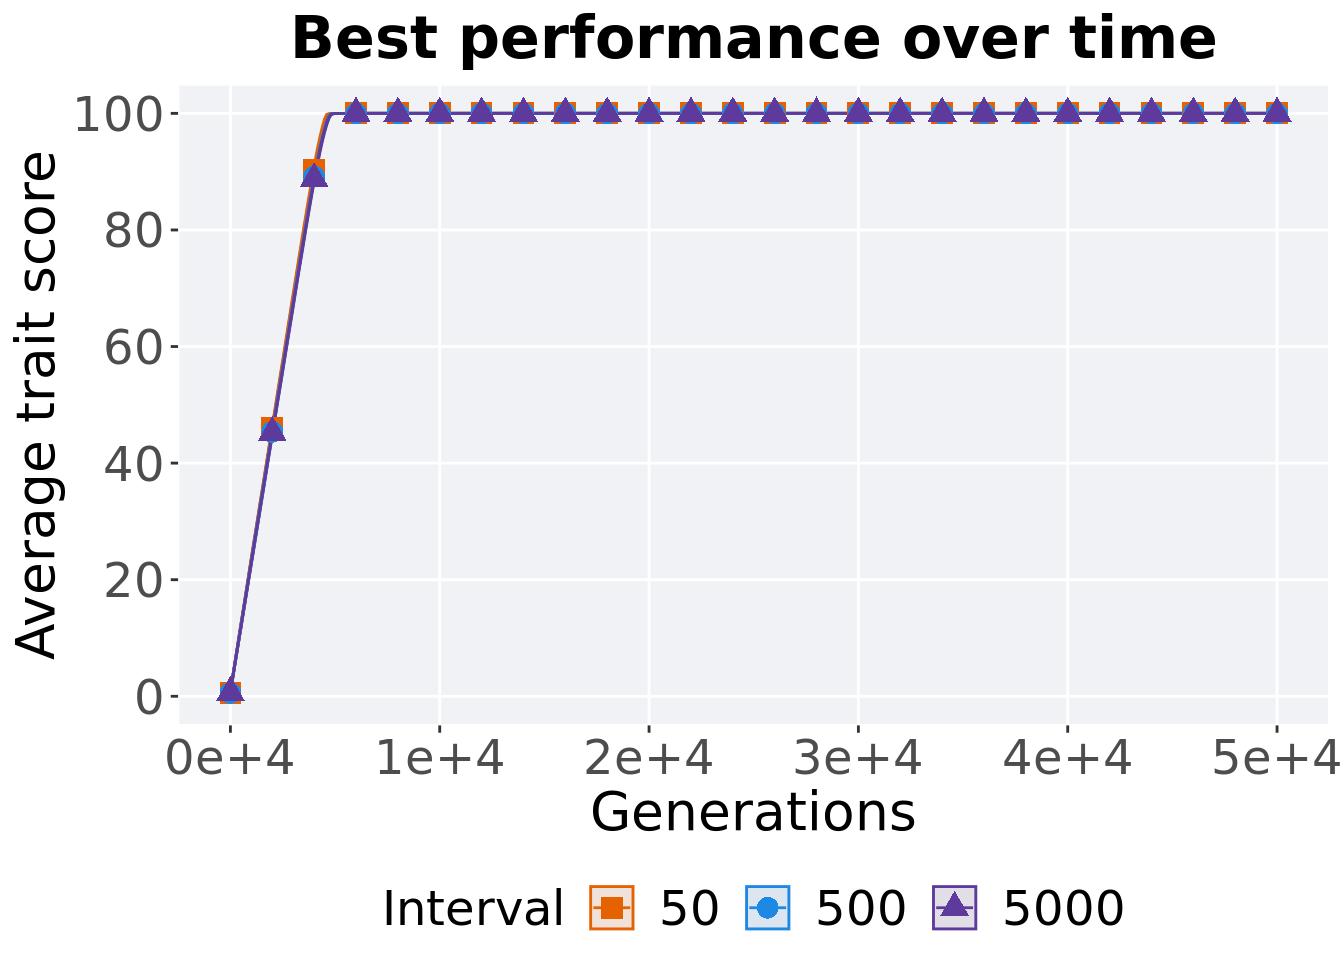
\includegraphics{demo_files/figure-latex/int-tru-exp-perf-1.pdf}

\hypertarget{generation-satisfactory-solution-found}{%
\subsection{Generation satisfactory solution found}\label{generation-satisfactory-solution-found}}

First generation a satisfactory solution is found throughout the 50,000 generations.

\begin{Shaded}
\begin{Highlighting}[]
\KeywordTok{filter}\NormalTok{(df_ssf, }\StringTok{`}\DataTypeTok{Selection}\CharTok{\textbackslash{}n}\DataTypeTok{Scheme}\StringTok{`} \OperatorTok{==}\StringTok{ 'TRUNCATION'}\NormalTok{) }\OperatorTok
\StringTok{  }\KeywordTok{ggplot}\NormalTok{(., }\KeywordTok{aes}\NormalTok{(}\DataTypeTok{x =}\NormalTok{ Interval, }\DataTypeTok{y =}\NormalTok{ Generations, }\DataTypeTok{color =}\NormalTok{ Interval, }\DataTypeTok{fill =}\NormalTok{ Interval, }\DataTypeTok{shape =}\NormalTok{ Interval)) }\OperatorTok{+}
\StringTok{  }\KeywordTok{geom_flat_violin}\NormalTok{(}\DataTypeTok{position =} \KeywordTok{position_nudge}\NormalTok{(}\DataTypeTok{x =} \FloatTok{.09}\NormalTok{, }\DataTypeTok{y =} \DecValTok{0}\NormalTok{), }\DataTypeTok{scale =} \StringTok{'width'}\NormalTok{, }\DataTypeTok{alpha =} \FloatTok{0.2}\NormalTok{, }\DataTypeTok{width =} \FloatTok{1.5}\NormalTok{) }\OperatorTok{+}
\StringTok{  }\KeywordTok{geom_boxplot}\NormalTok{(}\DataTypeTok{color =} \StringTok{'black'}\NormalTok{, }\DataTypeTok{width =} \FloatTok{.07}\NormalTok{, }\DataTypeTok{outlier.shape =} \OtherTok{NA}\NormalTok{, }\DataTypeTok{alpha =} \FloatTok{0.0}\NormalTok{, }\DataTypeTok{size =} \FloatTok{1.0}\NormalTok{, }\DataTypeTok{position =} \KeywordTok{position_nudge}\NormalTok{(}\DataTypeTok{x =} \FloatTok{.15}\NormalTok{, }\DataTypeTok{y =} \DecValTok{0}\NormalTok{)) }\OperatorTok{+}
\StringTok{  }\KeywordTok{geom_point}\NormalTok{(}\DataTypeTok{position =} \KeywordTok{position_jitter}\NormalTok{(}\DataTypeTok{width =} \FloatTok{.02}\NormalTok{), }\DataTypeTok{size =} \FloatTok{3.0}\NormalTok{, }\DataTypeTok{alpha =} \FloatTok{1.0}\NormalTok{) }\OperatorTok{+}
\StringTok{  }\KeywordTok{scale_shape_manual}\NormalTok{(}\DataTypeTok{values=}\NormalTok{SHAPE)}\OperatorTok{+}
\StringTok{  }\KeywordTok{scale_y_continuous}\NormalTok{(}
    \DataTypeTok{name=}\StringTok{"Generations"}
\NormalTok{  ) }\OperatorTok{+}
\StringTok{  }\KeywordTok{scale_x_discrete}\NormalTok{(}
    \DataTypeTok{name=}\StringTok{"Interval"}
\NormalTok{  ) }\OperatorTok{+}
\StringTok{  }\KeywordTok{scale_colour_manual}\NormalTok{(}\DataTypeTok{values =}\NormalTok{ cb_palette_mi) }\OperatorTok{+}
\StringTok{  }\KeywordTok{scale_fill_manual}\NormalTok{(}\DataTypeTok{values =}\NormalTok{ cb_palette_mi) }\OperatorTok{+}
\StringTok{  }\NormalTok{p_theme}
\end{Highlighting}
\end{Shaded}

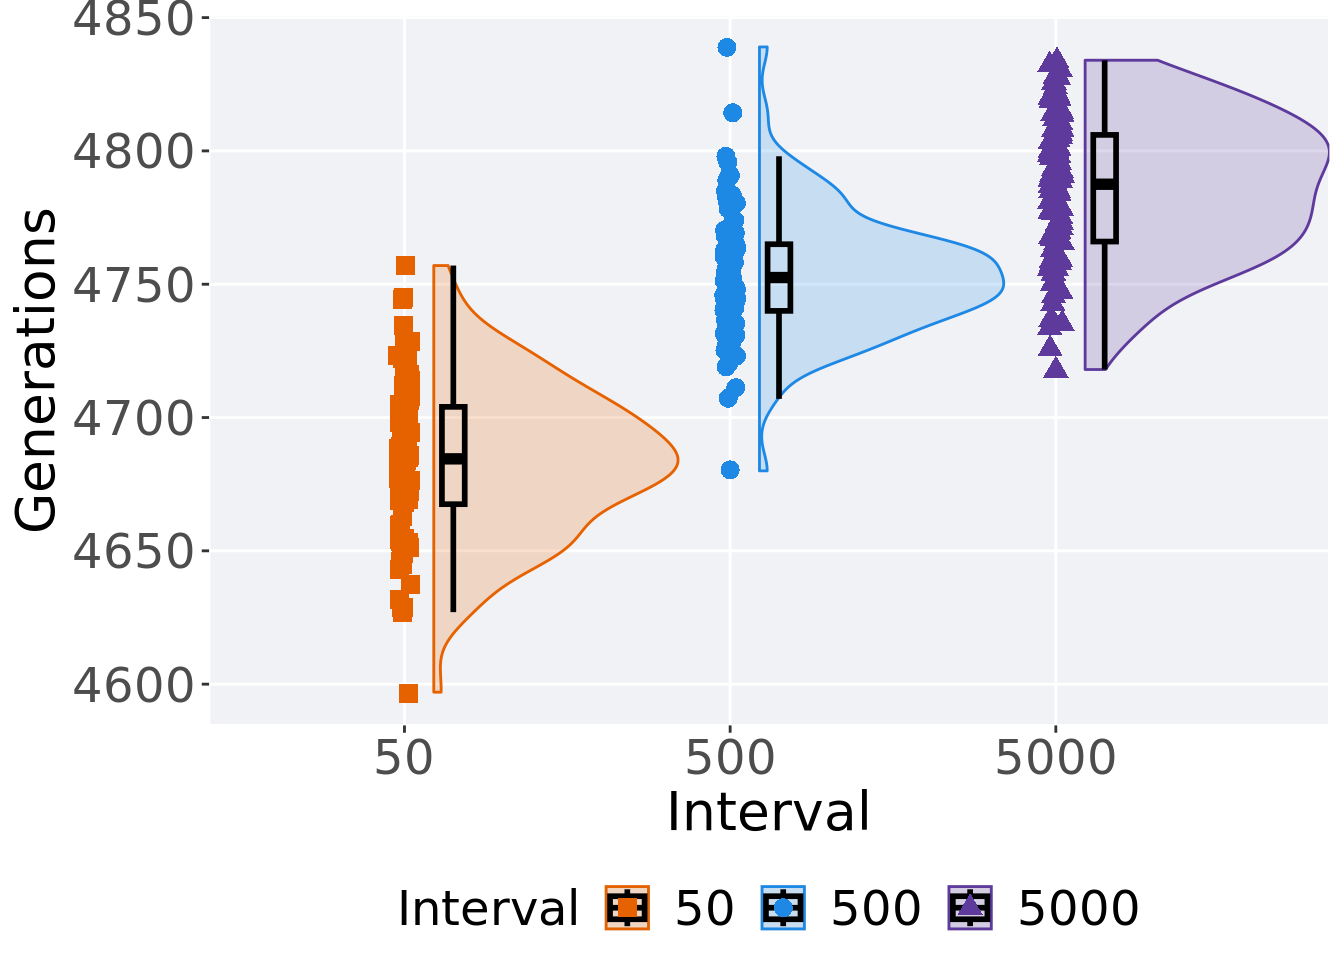
\includegraphics{demo_files/figure-latex/int-tru-exp-ssf-1.pdf}

\hypertarget{stats}{%
\subsection{Stats}\label{stats}}

Summary statistics for the first generation a satisfactory solution is found.

\begin{Shaded}
\begin{Highlighting}[]
\NormalTok{ssf =}\StringTok{ }\KeywordTok{filter}\NormalTok{(df_ssf, }\StringTok{`}\DataTypeTok{Selection}\CharTok{\textbackslash{}n}\DataTypeTok{Scheme}\StringTok{`} \OperatorTok{==}\StringTok{ 'TRUNCATION'}\NormalTok{)}
\NormalTok{ssf }\OperatorTok
\StringTok{  }\KeywordTok{group_by}\NormalTok{(Interval) }\OperatorTok
\StringTok{  }\NormalTok{dplyr}\OperatorTok{::}\KeywordTok{summarise}\NormalTok{(}
    \DataTypeTok{count =} \KeywordTok{n}\NormalTok{(),}
    \DataTypeTok{na_cnt =} \KeywordTok{sum}\NormalTok{(}\KeywordTok{is.na}\NormalTok{(Generations)),}
    \DataTypeTok{min =} \KeywordTok{min}\NormalTok{(Generations, }\DataTypeTok{na.rm =} \OtherTok{TRUE}\NormalTok{),}
    \DataTypeTok{median =} \KeywordTok{median}\NormalTok{(Generations, }\DataTypeTok{na.rm =} \OtherTok{TRUE}\NormalTok{),}
    \DataTypeTok{mean =} \KeywordTok{mean}\NormalTok{(Generations, }\DataTypeTok{na.rm =} \OtherTok{TRUE}\NormalTok{),}
    \DataTypeTok{max =} \KeywordTok{max}\NormalTok{(Generations, }\DataTypeTok{na.rm =} \OtherTok{TRUE}\NormalTok{),}
    \DataTypeTok{IQR =} \KeywordTok{IQR}\NormalTok{(Generations, }\DataTypeTok{na.rm =} \OtherTok{TRUE}\NormalTok{)}
\NormalTok{  )}
\end{Highlighting}
\end{Shaded}

\begin{verbatim}
## # A tibble: 3 x 8
##   Interval count na_cnt   min median  mean   max   IQR
##   <fct>    <int>  <int> <int>  <dbl> <dbl> <int> <dbl>
## 1 50         100      0  4597  4684. 4684.  4757  36.5
## 2 500        100      0  4680  4752. 4754.  4839  25  
## 3 5000       100      0  4718  4788. 4786.  4834  40
\end{verbatim}

Kruskal--Wallis test provides evidence of difference among selection schemes.

\begin{Shaded}
\begin{Highlighting}[]
\KeywordTok{kruskal.test}\NormalTok{(Generations }\OperatorTok{~}\StringTok{ }\NormalTok{Interval, }\DataTypeTok{data =}\NormalTok{ ssf)}
\end{Highlighting}
\end{Shaded}

\begin{verbatim}
## 
##  Kruskal-Wallis rank sum test
## 
## data:  Generations by Interval
## Kruskal-Wallis chi-squared = 216.76, df = 2, p-value < 2.2e-16
\end{verbatim}

Results for post-hoc Wilcoxon rank-sum test with a Bonferroni correction.

\begin{Shaded}
\begin{Highlighting}[]
\KeywordTok{pairwise.wilcox.test}\NormalTok{(}\DataTypeTok{x =}\NormalTok{ ssf}\OperatorTok{$}\NormalTok{Generations, }\DataTypeTok{g =}\NormalTok{ ssf}\OperatorTok{$}\NormalTok{Interval, }\DataTypeTok{p.adjust.method =} \StringTok{"bonferroni"}\NormalTok{,}
                     \DataTypeTok{paired =} \OtherTok{FALSE}\NormalTok{, }\DataTypeTok{conf.int =} \OtherTok{FALSE}\NormalTok{, }\DataTypeTok{alternative =} \StringTok{'g'}\NormalTok{)}
\end{Highlighting}
\end{Shaded}

\begin{verbatim}
## 
##  Pairwise comparisons using Wilcoxon rank sum test with continuity correction 
## 
## data:  ssf$Generations and ssf$Interval 
## 
##      50      500    
## 500  < 2e-16 -      
## 5000 < 2e-16 7.6e-15
## 
## P value adjustment method: bonferroni
\end{verbatim}

\hypertarget{tournament-selection}{%
\section{Tournament selection}\label{tournament-selection}}

Here we analyze how the different migration intervals affect tournament selection on the exploitation rate diagnostic.

\hypertarget{performance-over-time-1}{%
\subsection{Performance over time}\label{performance-over-time-1}}

\begin{Shaded}
\begin{Highlighting}[]
\NormalTok{lines =}\StringTok{ }\KeywordTok{filter}\NormalTok{(df_ot, }\StringTok{`}\DataTypeTok{Selection}\CharTok{\textbackslash{}n}\DataTypeTok{Scheme}\StringTok{`} \OperatorTok{==}\StringTok{ 'TOURNAMENT'}\NormalTok{) }\OperatorTok
\StringTok{  }\KeywordTok{group_by}\NormalTok{(Interval, Generations) }\OperatorTok
\StringTok{  }\NormalTok{dplyr}\OperatorTok{::}\KeywordTok{summarise}\NormalTok{(}
    \DataTypeTok{min =} \KeywordTok{min}\NormalTok{(pop_fit_max) }\OperatorTok{/}\StringTok{ }\NormalTok{DIMENSIONALITY,}
    \DataTypeTok{mean =} \KeywordTok{mean}\NormalTok{(pop_fit_max) }\OperatorTok{/}\StringTok{ }\NormalTok{DIMENSIONALITY,}
    \DataTypeTok{max =} \KeywordTok{max}\NormalTok{(pop_fit_max) }\OperatorTok{/}\StringTok{ }\NormalTok{DIMENSIONALITY}
\NormalTok{  )}
\KeywordTok{ggplot}\NormalTok{(lines, }\KeywordTok{aes}\NormalTok{(}\DataTypeTok{x=}\NormalTok{Generations, }\DataTypeTok{y=}\NormalTok{mean, }\DataTypeTok{group =}\NormalTok{ Interval, }\DataTypeTok{fill =}\NormalTok{ Interval, }\DataTypeTok{color =}\NormalTok{ Interval, }\DataTypeTok{shape =}\NormalTok{ Interval)) }\OperatorTok{+}
\StringTok{  }\KeywordTok{geom_ribbon}\NormalTok{(}\KeywordTok{aes}\NormalTok{(}\DataTypeTok{ymin =}\NormalTok{ min, }\DataTypeTok{ymax =}\NormalTok{ max), }\DataTypeTok{alpha =} \FloatTok{0.1}\NormalTok{) }\OperatorTok{+}
\StringTok{  }\KeywordTok{geom_line}\NormalTok{(}\DataTypeTok{size =} \FloatTok{0.5}\NormalTok{) }\OperatorTok{+}
\StringTok{  }\KeywordTok{geom_point}\NormalTok{(}\DataTypeTok{data =} \KeywordTok{filter}\NormalTok{(lines, Generations }\OperatorTok\StringTok{ }\DecValTok{2000} \OperatorTok{==}\StringTok{ }\DecValTok{0}\NormalTok{), }\DataTypeTok{size =} \FloatTok{2.5}\NormalTok{, }\DataTypeTok{stroke =} \FloatTok{2.0}\NormalTok{, }\DataTypeTok{alpha =} \FloatTok{1.0}\NormalTok{) }\OperatorTok{+}
\StringTok{  }\KeywordTok{scale_y_continuous}\NormalTok{(}
    \DataTypeTok{name=}\StringTok{"Average trait score"}\NormalTok{,}
    \DataTypeTok{limits=}\KeywordTok{c}\NormalTok{(}\DecValTok{0}\NormalTok{, }\DecValTok{100}\NormalTok{),}
    \DataTypeTok{breaks=}\KeywordTok{seq}\NormalTok{(}\DecValTok{0}\NormalTok{,}\DecValTok{100}\NormalTok{, }\DecValTok{20}\NormalTok{),}
    \DataTypeTok{labels=}\KeywordTok{c}\NormalTok{(}\StringTok{"0"}\NormalTok{, }\StringTok{"20"}\NormalTok{, }\StringTok{"40"}\NormalTok{, }\StringTok{"60"}\NormalTok{, }\StringTok{"80"}\NormalTok{, }\StringTok{"100"}\NormalTok{)}
\NormalTok{  ) }\OperatorTok{+}
\StringTok{  }\KeywordTok{scale_x_continuous}\NormalTok{(}
    \DataTypeTok{name=}\StringTok{"Generations"}\NormalTok{,}
    \DataTypeTok{limits=}\KeywordTok{c}\NormalTok{(}\DecValTok{0}\NormalTok{, }\DecValTok{50000}\NormalTok{),}
    \DataTypeTok{breaks=}\KeywordTok{c}\NormalTok{(}\DecValTok{0}\NormalTok{, }\DecValTok{10000}\NormalTok{, }\DecValTok{20000}\NormalTok{, }\DecValTok{30000}\NormalTok{, }\DecValTok{40000}\NormalTok{, }\DecValTok{50000}\NormalTok{),}
    \DataTypeTok{labels=}\KeywordTok{c}\NormalTok{(}\StringTok{"0e+4"}\NormalTok{, }\StringTok{"1e+4"}\NormalTok{, }\StringTok{"2e+4"}\NormalTok{, }\StringTok{"3e+4"}\NormalTok{, }\StringTok{"4e+4"}\NormalTok{, }\StringTok{"5e+4"}\NormalTok{)}

\NormalTok{  ) }\OperatorTok{+}
\StringTok{  }\KeywordTok{scale_shape_manual}\NormalTok{(}\DataTypeTok{values=}\NormalTok{SHAPE)}\OperatorTok{+}
\StringTok{  }\KeywordTok{scale_colour_manual}\NormalTok{(}\DataTypeTok{values =}\NormalTok{ cb_palette_mi) }\OperatorTok{+}
\StringTok{  }\KeywordTok{scale_fill_manual}\NormalTok{(}\DataTypeTok{values =}\NormalTok{ cb_palette_mi) }\OperatorTok{+}
\StringTok{  }\KeywordTok{ggtitle}\NormalTok{(}\StringTok{"Best performance over time"}\NormalTok{) }\OperatorTok{+}
\StringTok{  }\NormalTok{p_theme}
\end{Highlighting}
\end{Shaded}

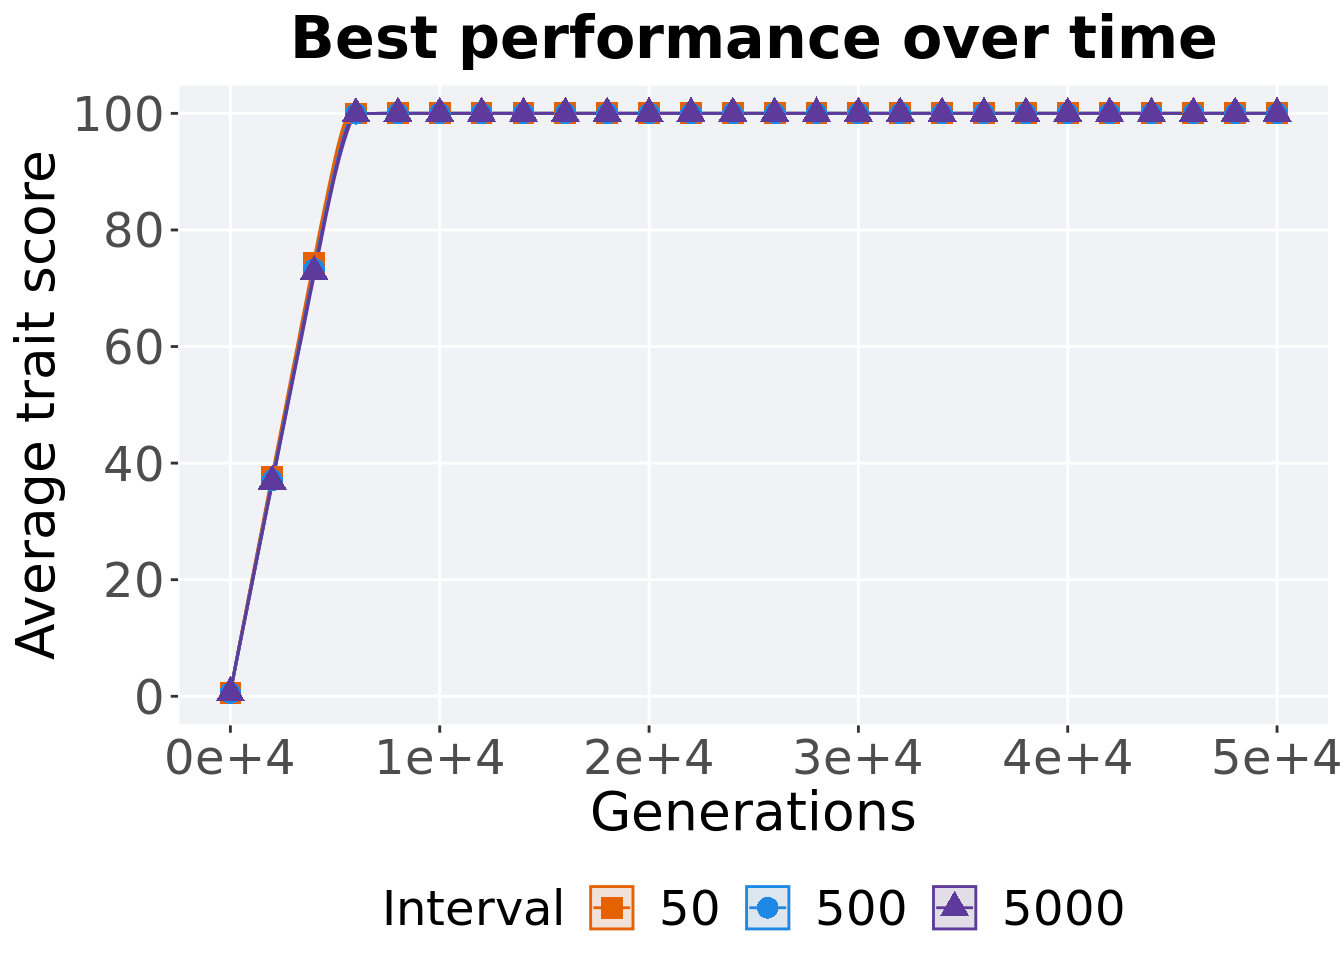
\includegraphics{demo_files/figure-latex/int-tor-exp-perf-1.pdf}

\hypertarget{generation-satisfactory-solution-found-1}{%
\subsection{Generation satisfactory solution found}\label{generation-satisfactory-solution-found-1}}

First generation a satisfactory solution is found throughout the 50,000 generations.

\begin{Shaded}
\begin{Highlighting}[]
\KeywordTok{filter}\NormalTok{(df_ssf, }\StringTok{`}\DataTypeTok{Selection}\CharTok{\textbackslash{}n}\DataTypeTok{Scheme}\StringTok{`} \OperatorTok{==}\StringTok{ 'TOURNAMENT'}\NormalTok{) }\OperatorTok
\StringTok{  }\KeywordTok{ggplot}\NormalTok{(., }\KeywordTok{aes}\NormalTok{(}\DataTypeTok{x =}\NormalTok{ Interval, }\DataTypeTok{y =}\NormalTok{ Generations, }\DataTypeTok{color =}\NormalTok{ Interval, }\DataTypeTok{fill =}\NormalTok{ Interval, }\DataTypeTok{shape =}\NormalTok{ Interval)) }\OperatorTok{+}
\StringTok{  }\KeywordTok{geom_flat_violin}\NormalTok{(}\DataTypeTok{position =} \KeywordTok{position_nudge}\NormalTok{(}\DataTypeTok{x =} \FloatTok{.09}\NormalTok{, }\DataTypeTok{y =} \DecValTok{0}\NormalTok{), }\DataTypeTok{scale =} \StringTok{'width'}\NormalTok{, }\DataTypeTok{alpha =} \FloatTok{0.2}\NormalTok{, }\DataTypeTok{width =} \FloatTok{1.5}\NormalTok{) }\OperatorTok{+}
\StringTok{  }\KeywordTok{geom_boxplot}\NormalTok{(}\DataTypeTok{color =} \StringTok{'black'}\NormalTok{, }\DataTypeTok{width =} \FloatTok{.07}\NormalTok{, }\DataTypeTok{outlier.shape =} \OtherTok{NA}\NormalTok{, }\DataTypeTok{alpha =} \FloatTok{0.0}\NormalTok{, }\DataTypeTok{size =} \FloatTok{1.0}\NormalTok{, }\DataTypeTok{position =} \KeywordTok{position_nudge}\NormalTok{(}\DataTypeTok{x =} \FloatTok{.15}\NormalTok{, }\DataTypeTok{y =} \DecValTok{0}\NormalTok{)) }\OperatorTok{+}
\StringTok{  }\KeywordTok{geom_point}\NormalTok{(}\DataTypeTok{position =} \KeywordTok{position_jitter}\NormalTok{(}\DataTypeTok{width =} \FloatTok{.02}\NormalTok{), }\DataTypeTok{size =} \FloatTok{3.0}\NormalTok{, }\DataTypeTok{alpha =} \FloatTok{1.0}\NormalTok{) }\OperatorTok{+}
\StringTok{  }\KeywordTok{scale_shape_manual}\NormalTok{(}\DataTypeTok{values=}\NormalTok{SHAPE)}\OperatorTok{+}
\StringTok{  }\KeywordTok{scale_y_continuous}\NormalTok{(}
    \DataTypeTok{name=}\StringTok{"Generations"}
\NormalTok{  ) }\OperatorTok{+}
\StringTok{  }\KeywordTok{scale_x_discrete}\NormalTok{(}
    \DataTypeTok{name=}\StringTok{"Interval"}
\NormalTok{  ) }\OperatorTok{+}
\StringTok{  }\KeywordTok{scale_colour_manual}\NormalTok{(}\DataTypeTok{values =}\NormalTok{ cb_palette_mi) }\OperatorTok{+}
\StringTok{  }\KeywordTok{scale_fill_manual}\NormalTok{(}\DataTypeTok{values =}\NormalTok{ cb_palette_mi) }\OperatorTok{+}
\StringTok{  }\NormalTok{p_theme}
\end{Highlighting}
\end{Shaded}

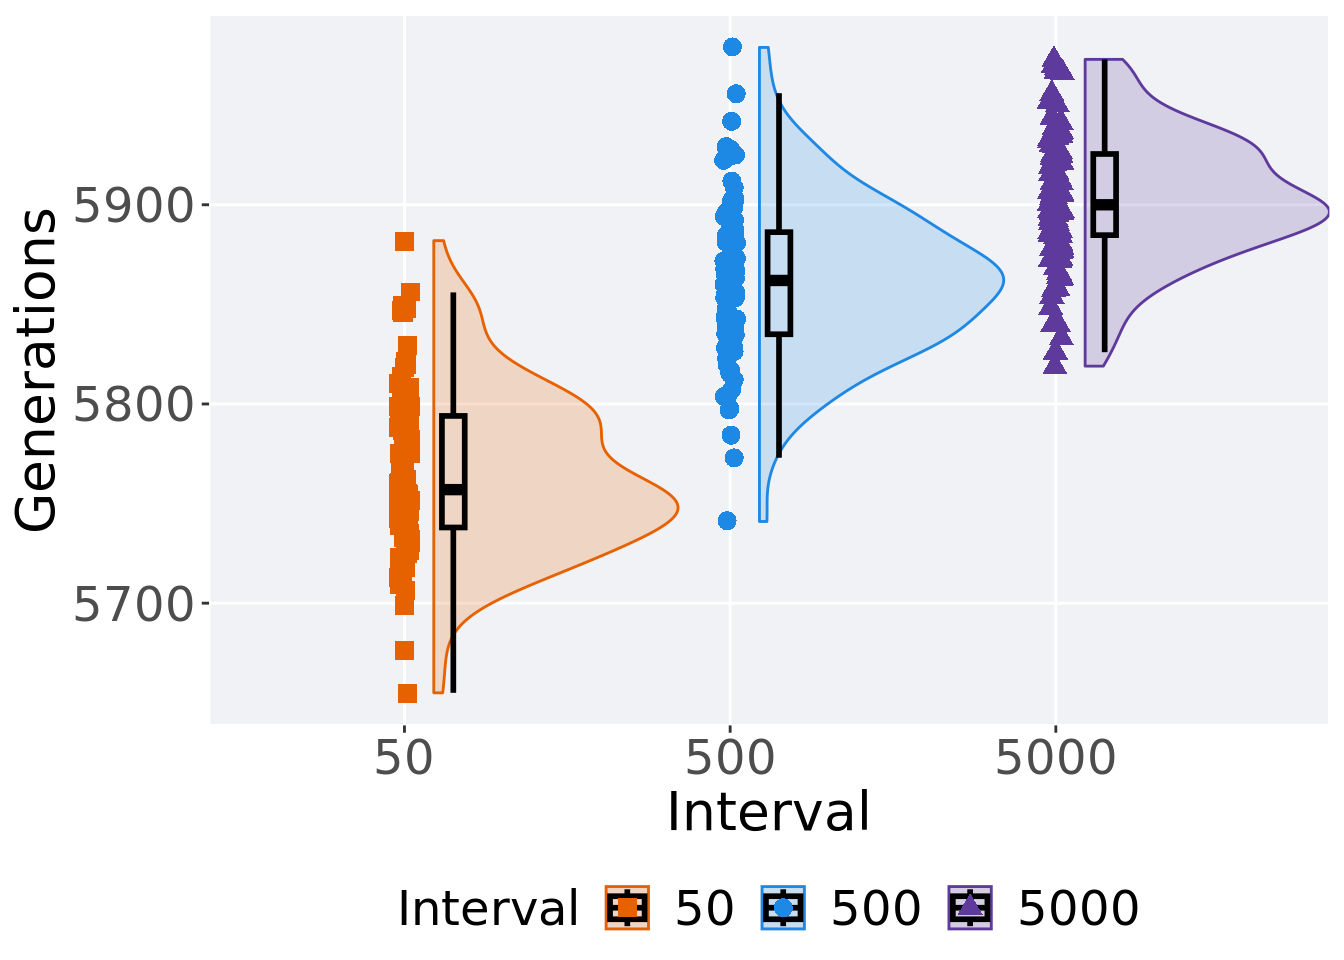
\includegraphics{demo_files/figure-latex/int-tor-exp-ssf-1.pdf}

\hypertarget{stats-1}{%
\subsection{Stats}\label{stats-1}}

Summary statistics for the first generation a satisfactory solution is found.

\begin{Shaded}
\begin{Highlighting}[]
\NormalTok{ssf =}\StringTok{ }\KeywordTok{filter}\NormalTok{(df_ssf, }\StringTok{`}\DataTypeTok{Selection}\CharTok{\textbackslash{}n}\DataTypeTok{Scheme}\StringTok{`} \OperatorTok{==}\StringTok{ 'TOURNAMENT'}\NormalTok{)}
\NormalTok{ssf }\OperatorTok
\StringTok{  }\KeywordTok{group_by}\NormalTok{(Interval) }\OperatorTok
\StringTok{  }\NormalTok{dplyr}\OperatorTok{::}\KeywordTok{summarise}\NormalTok{(}
    \DataTypeTok{count =} \KeywordTok{n}\NormalTok{(),}
    \DataTypeTok{na_cnt =} \KeywordTok{sum}\NormalTok{(}\KeywordTok{is.na}\NormalTok{(Generations)),}
    \DataTypeTok{min =} \KeywordTok{min}\NormalTok{(Generations, }\DataTypeTok{na.rm =} \OtherTok{TRUE}\NormalTok{),}
    \DataTypeTok{median =} \KeywordTok{median}\NormalTok{(Generations, }\DataTypeTok{na.rm =} \OtherTok{TRUE}\NormalTok{),}
    \DataTypeTok{mean =} \KeywordTok{mean}\NormalTok{(Generations, }\DataTypeTok{na.rm =} \OtherTok{TRUE}\NormalTok{),}
    \DataTypeTok{max =} \KeywordTok{max}\NormalTok{(Generations, }\DataTypeTok{na.rm =} \OtherTok{TRUE}\NormalTok{),}
    \DataTypeTok{IQR =} \KeywordTok{IQR}\NormalTok{(Generations, }\DataTypeTok{na.rm =} \OtherTok{TRUE}\NormalTok{)}
\NormalTok{  )}
\end{Highlighting}
\end{Shaded}

\begin{verbatim}
## # A tibble: 3 x 8
##   Interval count na_cnt   min median  mean   max   IQR
##   <fct>    <int>  <int> <int>  <dbl> <dbl> <int> <dbl>
## 1 50         100      0  5655   5757 5765.  5882  56  
## 2 500        100      0  5741   5862 5862.  5979  51.2
## 3 5000       100      0  5819   5900 5903.  5973  40.8
\end{verbatim}

Kruskal--Wallis test provides evidence of difference among selection schemes.

\begin{Shaded}
\begin{Highlighting}[]
\KeywordTok{kruskal.test}\NormalTok{(Generations }\OperatorTok{~}\StringTok{ }\NormalTok{Interval, }\DataTypeTok{data =}\NormalTok{ ssf)}
\end{Highlighting}
\end{Shaded}

\begin{verbatim}
## 
##  Kruskal-Wallis rank sum test
## 
## data:  Generations by Interval
## Kruskal-Wallis chi-squared = 203.85, df = 2, p-value < 2.2e-16
\end{verbatim}

Results for post-hoc Wilcoxon rank-sum test with a Bonferroni correction.

\begin{Shaded}
\begin{Highlighting}[]
\KeywordTok{pairwise.wilcox.test}\NormalTok{(}\DataTypeTok{x =}\NormalTok{ ssf}\OperatorTok{$}\NormalTok{Generations, }\DataTypeTok{g =}\NormalTok{ ssf}\OperatorTok{$}\NormalTok{Interval, }\DataTypeTok{p.adjust.method =} \StringTok{"bonferroni"}\NormalTok{,}
                     \DataTypeTok{paired =} \OtherTok{FALSE}\NormalTok{, }\DataTypeTok{conf.int =} \OtherTok{FALSE}\NormalTok{, }\DataTypeTok{alternative =} \StringTok{'g'}\NormalTok{)}
\end{Highlighting}
\end{Shaded}

\begin{verbatim}
## 
##  Pairwise comparisons using Wilcoxon rank sum test with continuity correction 
## 
## data:  ssf$Generations and ssf$Interval 
## 
##      50     500  
## 500  <2e-16 -    
## 5000 <2e-16 1e-12
## 
## P value adjustment method: bonferroni
\end{verbatim}

\hypertarget{lexicase-selection}{%
\section{Lexicase selection}\label{lexicase-selection}}

Here we analyze how the different migration intervals affect tournament selection on the exploitation rate diagnostic.

\hypertarget{performance-over-time-2}{%
\subsection{Performance over time}\label{performance-over-time-2}}

\begin{Shaded}
\begin{Highlighting}[]
\NormalTok{lines =}\StringTok{ }\KeywordTok{filter}\NormalTok{(df_ot, }\StringTok{`}\DataTypeTok{Selection}\CharTok{\textbackslash{}n}\DataTypeTok{Scheme}\StringTok{`} \OperatorTok{==}\StringTok{ 'LEXICASE'}\NormalTok{) }\OperatorTok
\StringTok{  }\KeywordTok{group_by}\NormalTok{(Interval, Generations) }\OperatorTok
\StringTok{  }\NormalTok{dplyr}\OperatorTok{::}\KeywordTok{summarise}\NormalTok{(}
    \DataTypeTok{min =} \KeywordTok{min}\NormalTok{(pop_fit_max) }\OperatorTok{/}\StringTok{ }\NormalTok{DIMENSIONALITY,}
    \DataTypeTok{mean =} \KeywordTok{mean}\NormalTok{(pop_fit_max) }\OperatorTok{/}\StringTok{ }\NormalTok{DIMENSIONALITY,}
    \DataTypeTok{max =} \KeywordTok{max}\NormalTok{(pop_fit_max) }\OperatorTok{/}\StringTok{ }\NormalTok{DIMENSIONALITY}
\NormalTok{  )}
\KeywordTok{ggplot}\NormalTok{(lines, }\KeywordTok{aes}\NormalTok{(}\DataTypeTok{x=}\NormalTok{Generations, }\DataTypeTok{y=}\NormalTok{mean, }\DataTypeTok{group =}\NormalTok{ Interval, }\DataTypeTok{fill =}\NormalTok{ Interval, }\DataTypeTok{color =}\NormalTok{ Interval, }\DataTypeTok{shape =}\NormalTok{ Interval)) }\OperatorTok{+}
\StringTok{  }\KeywordTok{geom_ribbon}\NormalTok{(}\KeywordTok{aes}\NormalTok{(}\DataTypeTok{ymin =}\NormalTok{ min, }\DataTypeTok{ymax =}\NormalTok{ max), }\DataTypeTok{alpha =} \FloatTok{0.1}\NormalTok{) }\OperatorTok{+}
\StringTok{  }\KeywordTok{geom_line}\NormalTok{(}\DataTypeTok{size =} \FloatTok{0.5}\NormalTok{) }\OperatorTok{+}
\StringTok{  }\KeywordTok{geom_point}\NormalTok{(}\DataTypeTok{data =} \KeywordTok{filter}\NormalTok{(lines, Generations }\OperatorTok\StringTok{ }\DecValTok{2000} \OperatorTok{==}\StringTok{ }\DecValTok{0}\NormalTok{), }\DataTypeTok{size =} \FloatTok{2.5}\NormalTok{, }\DataTypeTok{stroke =} \FloatTok{2.0}\NormalTok{, }\DataTypeTok{alpha =} \FloatTok{1.0}\NormalTok{) }\OperatorTok{+}
\StringTok{  }\KeywordTok{scale_y_continuous}\NormalTok{(}
    \DataTypeTok{name=}\StringTok{"Average trait score"}\NormalTok{,}
    \DataTypeTok{limits=}\KeywordTok{c}\NormalTok{(}\DecValTok{0}\NormalTok{, }\DecValTok{100}\NormalTok{),}
    \DataTypeTok{breaks=}\KeywordTok{seq}\NormalTok{(}\DecValTok{0}\NormalTok{,}\DecValTok{100}\NormalTok{, }\DecValTok{20}\NormalTok{),}
    \DataTypeTok{labels=}\KeywordTok{c}\NormalTok{(}\StringTok{"0"}\NormalTok{, }\StringTok{"20"}\NormalTok{, }\StringTok{"40"}\NormalTok{, }\StringTok{"60"}\NormalTok{, }\StringTok{"80"}\NormalTok{, }\StringTok{"100"}\NormalTok{)}
\NormalTok{  ) }\OperatorTok{+}
\StringTok{  }\KeywordTok{scale_x_continuous}\NormalTok{(}
    \DataTypeTok{name=}\StringTok{"Generations"}\NormalTok{,}
    \DataTypeTok{limits=}\KeywordTok{c}\NormalTok{(}\DecValTok{0}\NormalTok{, }\DecValTok{50000}\NormalTok{),}
    \DataTypeTok{breaks=}\KeywordTok{c}\NormalTok{(}\DecValTok{0}\NormalTok{, }\DecValTok{10000}\NormalTok{, }\DecValTok{20000}\NormalTok{, }\DecValTok{30000}\NormalTok{, }\DecValTok{40000}\NormalTok{, }\DecValTok{50000}\NormalTok{),}
    \DataTypeTok{labels=}\KeywordTok{c}\NormalTok{(}\StringTok{"0e+4"}\NormalTok{, }\StringTok{"1e+4"}\NormalTok{, }\StringTok{"2e+4"}\NormalTok{, }\StringTok{"3e+4"}\NormalTok{, }\StringTok{"4e+4"}\NormalTok{, }\StringTok{"5e+4"}\NormalTok{)}

\NormalTok{  ) }\OperatorTok{+}
\StringTok{  }\KeywordTok{scale_shape_manual}\NormalTok{(}\DataTypeTok{values=}\NormalTok{SHAPE)}\OperatorTok{+}
\StringTok{  }\KeywordTok{scale_colour_manual}\NormalTok{(}\DataTypeTok{values =}\NormalTok{ cb_palette_mi) }\OperatorTok{+}
\StringTok{  }\KeywordTok{scale_fill_manual}\NormalTok{(}\DataTypeTok{values =}\NormalTok{ cb_palette_mi) }\OperatorTok{+}
\StringTok{  }\KeywordTok{ggtitle}\NormalTok{(}\StringTok{"Best performance over time"}\NormalTok{) }\OperatorTok{+}
\StringTok{  }\NormalTok{p_theme}
\end{Highlighting}
\end{Shaded}

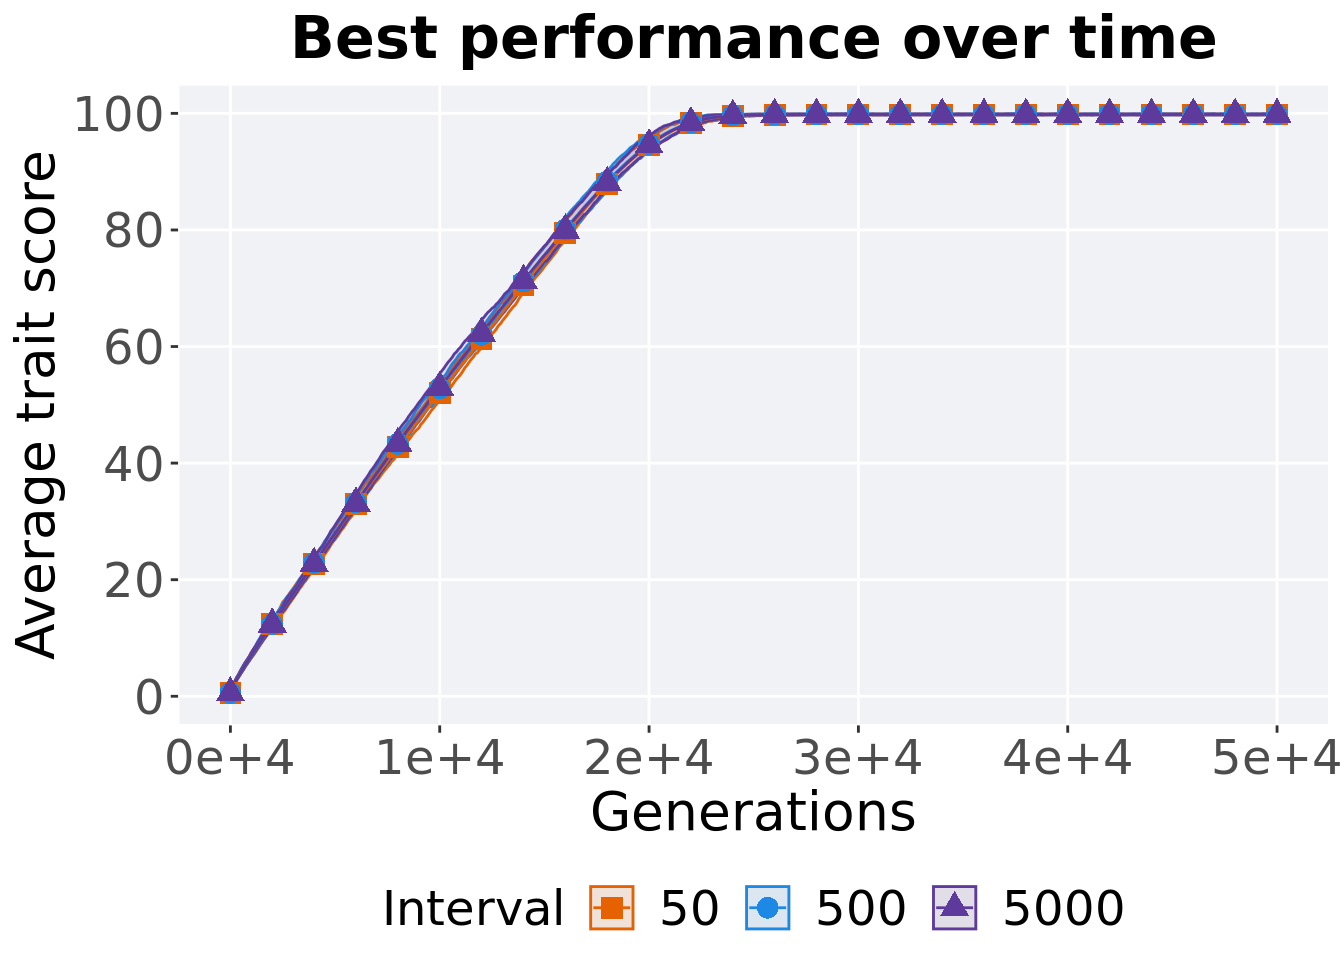
\includegraphics{demo_files/figure-latex/int-lex-exp-perf-1.pdf}

\hypertarget{generation-satisfactory-solution-found-2}{%
\subsection{Generation satisfactory solution found}\label{generation-satisfactory-solution-found-2}}

First generation a satisfactory solution is found throughout the 50,000 generations.

\begin{Shaded}
\begin{Highlighting}[]
\KeywordTok{filter}\NormalTok{(df_ssf, }\StringTok{`}\DataTypeTok{Selection}\CharTok{\textbackslash{}n}\DataTypeTok{Scheme}\StringTok{`} \OperatorTok{==}\StringTok{ 'LEXICASE'}\NormalTok{) }\OperatorTok
\StringTok{  }\KeywordTok{ggplot}\NormalTok{(., }\KeywordTok{aes}\NormalTok{(}\DataTypeTok{x =}\NormalTok{ Interval, }\DataTypeTok{y =}\NormalTok{ Generations, }\DataTypeTok{color =}\NormalTok{ Interval, }\DataTypeTok{fill =}\NormalTok{ Interval, }\DataTypeTok{shape =}\NormalTok{ Interval)) }\OperatorTok{+}
\StringTok{  }\KeywordTok{geom_flat_violin}\NormalTok{(}\DataTypeTok{position =} \KeywordTok{position_nudge}\NormalTok{(}\DataTypeTok{x =} \FloatTok{.09}\NormalTok{, }\DataTypeTok{y =} \DecValTok{0}\NormalTok{), }\DataTypeTok{scale =} \StringTok{'width'}\NormalTok{, }\DataTypeTok{alpha =} \FloatTok{0.2}\NormalTok{, }\DataTypeTok{width =} \FloatTok{1.5}\NormalTok{) }\OperatorTok{+}
\StringTok{  }\KeywordTok{geom_boxplot}\NormalTok{(}\DataTypeTok{color =} \StringTok{'black'}\NormalTok{, }\DataTypeTok{width =} \FloatTok{.07}\NormalTok{, }\DataTypeTok{outlier.shape =} \OtherTok{NA}\NormalTok{, }\DataTypeTok{alpha =} \FloatTok{0.0}\NormalTok{, }\DataTypeTok{size =} \FloatTok{1.0}\NormalTok{, }\DataTypeTok{position =} \KeywordTok{position_nudge}\NormalTok{(}\DataTypeTok{x =} \FloatTok{.15}\NormalTok{, }\DataTypeTok{y =} \DecValTok{0}\NormalTok{)) }\OperatorTok{+}
\StringTok{  }\KeywordTok{geom_point}\NormalTok{(}\DataTypeTok{position =} \KeywordTok{position_jitter}\NormalTok{(}\DataTypeTok{width =} \FloatTok{.02}\NormalTok{), }\DataTypeTok{size =} \FloatTok{3.0}\NormalTok{, }\DataTypeTok{alpha =} \FloatTok{1.0}\NormalTok{) }\OperatorTok{+}
\StringTok{  }\KeywordTok{scale_shape_manual}\NormalTok{(}\DataTypeTok{values=}\NormalTok{SHAPE)}\OperatorTok{+}
\StringTok{  }\KeywordTok{scale_y_continuous}\NormalTok{(}
    \DataTypeTok{name=}\StringTok{"Generations"}
\NormalTok{  ) }\OperatorTok{+}
\StringTok{  }\KeywordTok{scale_x_discrete}\NormalTok{(}
    \DataTypeTok{name=}\StringTok{"Interval"}
\NormalTok{  ) }\OperatorTok{+}
\StringTok{  }\KeywordTok{scale_colour_manual}\NormalTok{(}\DataTypeTok{values =}\NormalTok{ cb_palette_mi) }\OperatorTok{+}
\StringTok{  }\KeywordTok{scale_fill_manual}\NormalTok{(}\DataTypeTok{values =}\NormalTok{ cb_palette_mi) }\OperatorTok{+}
\StringTok{  }\NormalTok{p_theme}
\end{Highlighting}
\end{Shaded}

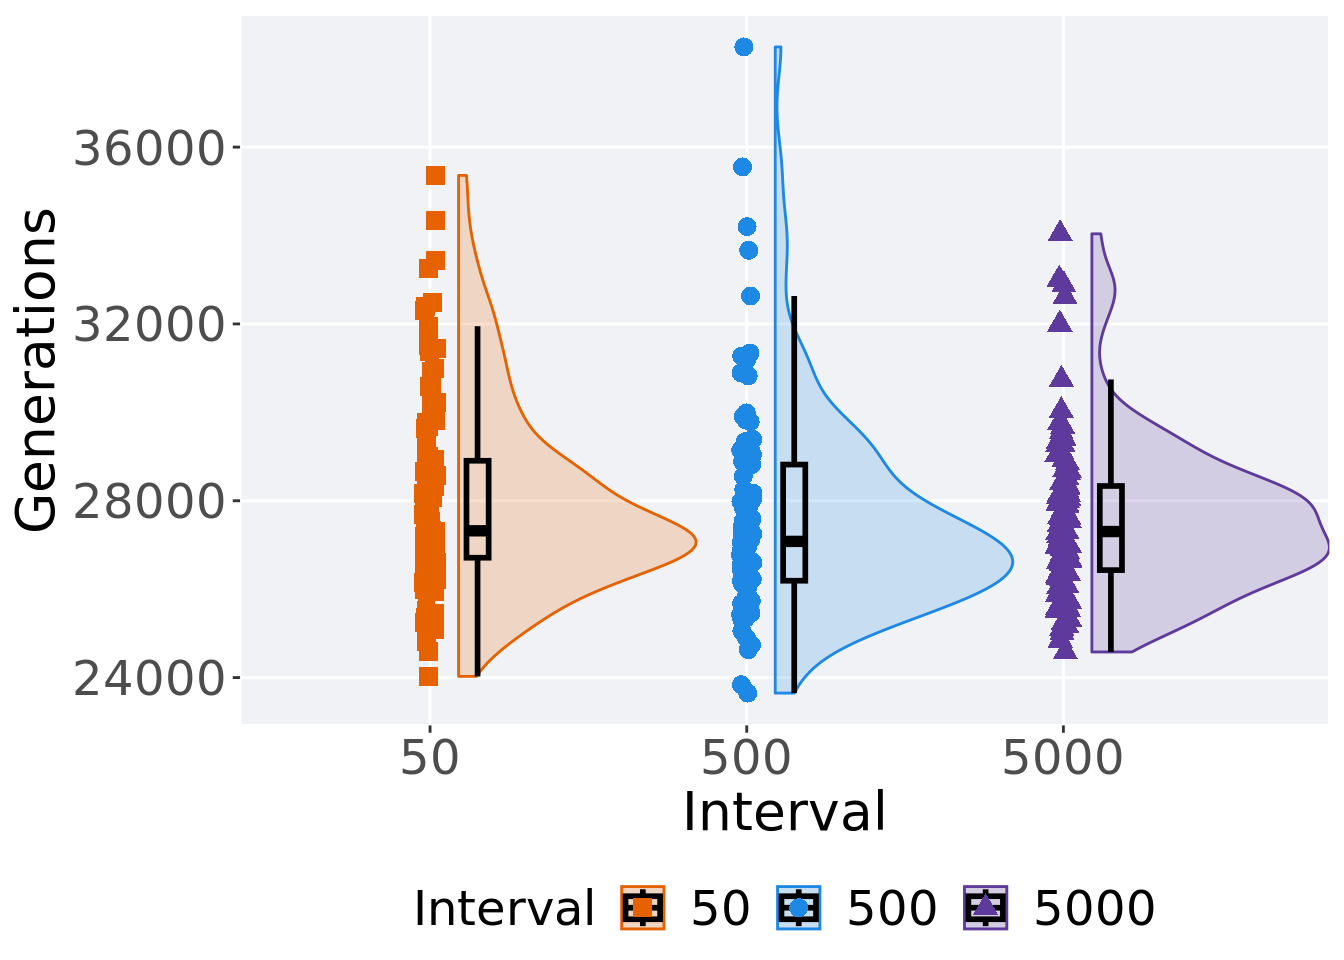
\includegraphics{demo_files/figure-latex/int-lex-exp-ssf-1.pdf}

\hypertarget{stats-2}{%
\subsection{Stats}\label{stats-2}}

Summary statistics for the first generation a satisfactory solution is found.

\begin{Shaded}
\begin{Highlighting}[]
\NormalTok{ssf =}\StringTok{ }\KeywordTok{filter}\NormalTok{(df_ssf, }\StringTok{`}\DataTypeTok{Selection}\CharTok{\textbackslash{}n}\DataTypeTok{Scheme}\StringTok{`} \OperatorTok{==}\StringTok{ 'LEXICASE'}\NormalTok{)}
\NormalTok{ssf }\OperatorTok
\StringTok{  }\KeywordTok{group_by}\NormalTok{(Interval) }\OperatorTok
\StringTok{  }\NormalTok{dplyr}\OperatorTok{::}\KeywordTok{summarise}\NormalTok{(}
    \DataTypeTok{count =} \KeywordTok{n}\NormalTok{(),}
    \DataTypeTok{na_cnt =} \KeywordTok{sum}\NormalTok{(}\KeywordTok{is.na}\NormalTok{(Generations)),}
    \DataTypeTok{min =} \KeywordTok{min}\NormalTok{(Generations, }\DataTypeTok{na.rm =} \OtherTok{TRUE}\NormalTok{),}
    \DataTypeTok{median =} \KeywordTok{median}\NormalTok{(Generations, }\DataTypeTok{na.rm =} \OtherTok{TRUE}\NormalTok{),}
    \DataTypeTok{mean =} \KeywordTok{mean}\NormalTok{(Generations, }\DataTypeTok{na.rm =} \OtherTok{TRUE}\NormalTok{),}
    \DataTypeTok{max =} \KeywordTok{max}\NormalTok{(Generations, }\DataTypeTok{na.rm =} \OtherTok{TRUE}\NormalTok{),}
    \DataTypeTok{IQR =} \KeywordTok{IQR}\NormalTok{(Generations, }\DataTypeTok{na.rm =} \OtherTok{TRUE}\NormalTok{)}
\NormalTok{  )}
\end{Highlighting}
\end{Shaded}

\begin{verbatim}
## # A tibble: 3 x 8
##   Interval count na_cnt   min median   mean   max   IQR
##   <fct>    <int>  <int> <int>  <dbl>  <dbl> <int> <dbl>
## 1 50         100      0 24027 27320  28031. 35360 2194.
## 2 500        100      0 23649 27080. 27635. 38266 2628.
## 3 5000       100      0 24579 27304. 27591. 34039 1903.
\end{verbatim}

Kruskal--Wallis test provides evidence of difference among selection schemes.

\begin{Shaded}
\begin{Highlighting}[]
\KeywordTok{kruskal.test}\NormalTok{(Generations }\OperatorTok{~}\StringTok{ }\NormalTok{Interval, }\DataTypeTok{data =}\NormalTok{ ssf)}
\end{Highlighting}
\end{Shaded}

\begin{verbatim}
## 
##  Kruskal-Wallis rank sum test
## 
## data:  Generations by Interval
## Kruskal-Wallis chi-squared = 3.1203, df = 2, p-value = 0.2101
\end{verbatim}

Results for post-hoc Wilcoxon rank-sum test with a Bonferroni correction.

\begin{Shaded}
\begin{Highlighting}[]
\KeywordTok{pairwise.wilcox.test}\NormalTok{(}\DataTypeTok{x =}\NormalTok{ ssf}\OperatorTok{$}\NormalTok{Generations, }\DataTypeTok{g =}\NormalTok{ ssf}\OperatorTok{$}\NormalTok{Interval, }\DataTypeTok{p.adjust.method =} \StringTok{"bonferroni"}\NormalTok{,}
                     \DataTypeTok{paired =} \OtherTok{FALSE}\NormalTok{, }\DataTypeTok{conf.int =} \OtherTok{FALSE}\NormalTok{, }\DataTypeTok{alternative =} \StringTok{'t'}\NormalTok{)}
\end{Highlighting}
\end{Shaded}

\begin{verbatim}
## 
##  Pairwise comparisons using Wilcoxon rank sum test with continuity correction 
## 
## data:  ssf$Generations and ssf$Interval 
## 
##      50   500 
## 500  0.27 -   
## 5000 0.73 1.00
## 
## P value adjustment method: bonferroni
\end{verbatim}

\hypertarget{interval-comparison-exploitation-rate-results-1}{%
\chapter{Interval comparison: Exploitation rate results}\label{interval-comparison-exploitation-rate-results-1}}

Here we present the results for \textbf{best performances} found by each selection scheme replicate on the exploitation rate diagnostic with our base configurations.
For our base configuration, we assume 4 islands and a ring topology.
When migrations occur, we swap two individuals (same position on each island) and guarantee that no solution can return to the same island.
Best performance found refers to the largest average trait score found in a given population.
Note that performance values fall between 0.0 and 100.0.

\hypertarget{analysis-dependencies-1}{%
\section{Analysis dependencies}\label{analysis-dependencies-1}}

\begin{Shaded}
\begin{Highlighting}[]
\KeywordTok{library}\NormalTok{(ggplot2)}
\KeywordTok{library}\NormalTok{(cowplot)}
\KeywordTok{library}\NormalTok{(dplyr)}
\KeywordTok{library}\NormalTok{(PupillometryR)}
\end{Highlighting}
\end{Shaded}

\hypertarget{data-1}{%
\section{Data}\label{data-1}}

\begin{Shaded}
\begin{Highlighting}[]
\NormalTok{base   =}\StringTok{ }\KeywordTok{filter}\NormalTok{(base_over_time,   Diagnostic }\OperatorTok{==}\StringTok{ 'ORDERED_EXPLOITATION'} \OperatorTok{&}\StringTok{ }\NormalTok{Structure }\OperatorTok{==}\StringTok{ 'IS'}\NormalTok{)}
\NormalTok{mi50   =}\StringTok{ }\KeywordTok{filter}\NormalTok{(mi50_over_time,   Diagnostic }\OperatorTok{==}\StringTok{ 'ORDERED_EXPLOITATION'} \OperatorTok{&}\StringTok{ }\NormalTok{Structure }\OperatorTok{==}\StringTok{ 'IS'}\NormalTok{)}
\NormalTok{mi5000 =}\StringTok{ }\KeywordTok{filter}\NormalTok{(mi5000_over_time, Diagnostic }\OperatorTok{==}\StringTok{ 'ORDERED_EXPLOITATION'} \OperatorTok{&}\StringTok{ }\NormalTok{Structure }\OperatorTok{==}\StringTok{ 'IS'}\NormalTok{)}

\NormalTok{base}\OperatorTok{$}\NormalTok{Interval =}\StringTok{ '500'}
\NormalTok{mi50}\OperatorTok{$}\NormalTok{Interval =}\StringTok{ '50'}
\NormalTok{mi5000}\OperatorTok{$}\NormalTok{Interval =}\StringTok{ '5000'}

\NormalTok{df_ot =}\StringTok{ }\KeywordTok{rbind}\NormalTok{(base, mi50, mi5000)}
\NormalTok{df_ot}\OperatorTok{$}\NormalTok{Interval =}\StringTok{ }\KeywordTok{factor}\NormalTok{(df_ot}\OperatorTok{$}\NormalTok{Interval, }\DataTypeTok{levels=}\KeywordTok{c}\NormalTok{(}\StringTok{'50'}\NormalTok{,}\StringTok{'500'}\NormalTok{,}\StringTok{'5000'}\NormalTok{))}


\NormalTok{base =}\StringTok{ }\KeywordTok{filter}\NormalTok{(base_ssf, Diagnostic }\OperatorTok{==}\StringTok{ 'ORDERED_EXPLOITATION'} \OperatorTok{&}\StringTok{ }\NormalTok{Structure }\OperatorTok{==}\StringTok{ 'IS'} \OperatorTok{&}\StringTok{ }\NormalTok{Generations }\OperatorTok{<}\StringTok{ }\DecValTok{60000}\NormalTok{)}
\NormalTok{mi50 =}\StringTok{ }\KeywordTok{filter}\NormalTok{(mi50_ssf, Diagnostic }\OperatorTok{==}\StringTok{ 'ORDERED_EXPLOITATION'} \OperatorTok{&}\StringTok{ }\NormalTok{Structure }\OperatorTok{==}\StringTok{ 'IS'} \OperatorTok{&}\StringTok{ }\NormalTok{Generations }\OperatorTok{<}\StringTok{ }\DecValTok{60000}\NormalTok{)}
\NormalTok{mi5000 =}\StringTok{ }\KeywordTok{filter}\NormalTok{(mi5000_ssf, Diagnostic }\OperatorTok{==}\StringTok{ 'ORDERED_EXPLOITATION'} \OperatorTok{&}\StringTok{ }\NormalTok{Structure }\OperatorTok{==}\StringTok{ 'IS'} \OperatorTok{&}\StringTok{ }\NormalTok{Generations }\OperatorTok{<}\StringTok{ }\DecValTok{60000}\NormalTok{)}

\NormalTok{base}\OperatorTok{$}\NormalTok{Interval =}\StringTok{ '500'}
\NormalTok{mi50}\OperatorTok{$}\NormalTok{Interval =}\StringTok{ '50'}
\NormalTok{mi5000}\OperatorTok{$}\NormalTok{Interval =}\StringTok{ '5000'}

\NormalTok{df_ssf =}\StringTok{ }\KeywordTok{rbind}\NormalTok{(mi50,base,mi5000)}
\NormalTok{df_ssf}\OperatorTok{$}\NormalTok{Interval =}\StringTok{ }\KeywordTok{factor}\NormalTok{(df_ssf}\OperatorTok{$}\NormalTok{Interval, }\DataTypeTok{levels =} \KeywordTok{c}\NormalTok{(}\StringTok{'50'}\NormalTok{,}\StringTok{'500'}\NormalTok{,}\StringTok{'5000'}\NormalTok{))}

\NormalTok{base =}\StringTok{ }\KeywordTok{filter}\NormalTok{(base_best, Diagnostic }\OperatorTok{==}\StringTok{ 'ORDERED_EXPLOITATION'} \OperatorTok{&}\StringTok{ }\NormalTok{Structure }\OperatorTok{==}\StringTok{ 'IS'} \OperatorTok{&}\StringTok{ }\NormalTok{Generations }\OperatorTok{<}\StringTok{ }\DecValTok{60000}\NormalTok{)}
\NormalTok{mi50 =}\StringTok{ }\KeywordTok{filter}\NormalTok{(mi50_best, Diagnostic }\OperatorTok{==}\StringTok{ 'ORDERED_EXPLOITATION'} \OperatorTok{&}\StringTok{ }\NormalTok{Structure }\OperatorTok{==}\StringTok{ 'IS'} \OperatorTok{&}\StringTok{ }\NormalTok{Generations }\OperatorTok{<}\StringTok{ }\DecValTok{60000}\NormalTok{)}
\NormalTok{mi5000 =}\StringTok{ }\KeywordTok{filter}\NormalTok{(mi5000_best, Diagnostic }\OperatorTok{==}\StringTok{ 'ORDERED_EXPLOITATION'} \OperatorTok{&}\StringTok{ }\NormalTok{Structure }\OperatorTok{==}\StringTok{ 'IS'} \OperatorTok{&}\StringTok{ }\NormalTok{Generations }\OperatorTok{<}\StringTok{ }\DecValTok{60000}\NormalTok{)}

\NormalTok{base}\OperatorTok{$}\NormalTok{Interval =}\StringTok{ '500'}
\NormalTok{mi50}\OperatorTok{$}\NormalTok{Interval =}\StringTok{ '50'}
\NormalTok{mi5000}\OperatorTok{$}\NormalTok{Interval =}\StringTok{ '5000'}

\NormalTok{df_best =}\StringTok{ }\KeywordTok{rbind}\NormalTok{(mi50,base,mi5000)}
\NormalTok{df_best}\OperatorTok{$}\NormalTok{Interval =}\StringTok{ }\KeywordTok{factor}\NormalTok{(df_best}\OperatorTok{$}\NormalTok{Interval, }\DataTypeTok{levels =} \KeywordTok{c}\NormalTok{(}\StringTok{'50'}\NormalTok{,}\StringTok{'500'}\NormalTok{,}\StringTok{'5000'}\NormalTok{))}
\end{Highlighting}
\end{Shaded}

\hypertarget{truncation-selection-1}{%
\section{Truncation selection}\label{truncation-selection-1}}

Here we analyze how the different migration intervals affect truncation selection on the exploitation rate diagnostic.

\hypertarget{performance-over-time-3}{%
\subsection{Performance over time}\label{performance-over-time-3}}

\begin{Shaded}
\begin{Highlighting}[]
\NormalTok{lines =}\StringTok{ }\KeywordTok{filter}\NormalTok{(df_ot, }\StringTok{`}\DataTypeTok{Selection}\CharTok{\textbackslash{}n}\DataTypeTok{Scheme}\StringTok{`} \OperatorTok{==}\StringTok{ 'TRUNCATION'}\NormalTok{) }\OperatorTok
\StringTok{  }\KeywordTok{group_by}\NormalTok{(Interval, Generations) }\OperatorTok
\StringTok{  }\NormalTok{dplyr}\OperatorTok{::}\KeywordTok{summarise}\NormalTok{(}
    \DataTypeTok{min =} \KeywordTok{min}\NormalTok{(pop_fit_max) }\OperatorTok{/}\StringTok{ }\NormalTok{DIMENSIONALITY,}
    \DataTypeTok{mean =} \KeywordTok{mean}\NormalTok{(pop_fit_max) }\OperatorTok{/}\StringTok{ }\NormalTok{DIMENSIONALITY,}
    \DataTypeTok{max =} \KeywordTok{max}\NormalTok{(pop_fit_max) }\OperatorTok{/}\StringTok{ }\NormalTok{DIMENSIONALITY}
\NormalTok{  )}
\KeywordTok{ggplot}\NormalTok{(lines, }\KeywordTok{aes}\NormalTok{(}\DataTypeTok{x=}\NormalTok{Generations, }\DataTypeTok{y=}\NormalTok{mean, }\DataTypeTok{group =}\NormalTok{ Interval, }\DataTypeTok{fill =}\NormalTok{ Interval, }\DataTypeTok{color =}\NormalTok{ Interval, }\DataTypeTok{shape =}\NormalTok{ Interval)) }\OperatorTok{+}
\StringTok{  }\KeywordTok{geom_ribbon}\NormalTok{(}\KeywordTok{aes}\NormalTok{(}\DataTypeTok{ymin =}\NormalTok{ min, }\DataTypeTok{ymax =}\NormalTok{ max), }\DataTypeTok{alpha =} \FloatTok{0.1}\NormalTok{) }\OperatorTok{+}
\StringTok{  }\KeywordTok{geom_line}\NormalTok{(}\DataTypeTok{size =} \FloatTok{0.5}\NormalTok{) }\OperatorTok{+}
\StringTok{  }\KeywordTok{geom_point}\NormalTok{(}\DataTypeTok{data =} \KeywordTok{filter}\NormalTok{(lines, Generations }\OperatorTok\StringTok{ }\DecValTok{2000} \OperatorTok{==}\StringTok{ }\DecValTok{0}\NormalTok{), }\DataTypeTok{size =} \FloatTok{2.5}\NormalTok{, }\DataTypeTok{stroke =} \FloatTok{2.0}\NormalTok{, }\DataTypeTok{alpha =} \FloatTok{1.0}\NormalTok{) }\OperatorTok{+}
\StringTok{  }\KeywordTok{scale_y_continuous}\NormalTok{(}
    \DataTypeTok{name=}\StringTok{"Average trait score"}\NormalTok{,}
    \DataTypeTok{limits=}\KeywordTok{c}\NormalTok{(}\DecValTok{0}\NormalTok{, }\DecValTok{100}\NormalTok{),}
    \DataTypeTok{breaks=}\KeywordTok{seq}\NormalTok{(}\DecValTok{0}\NormalTok{,}\DecValTok{100}\NormalTok{, }\DecValTok{20}\NormalTok{),}
    \DataTypeTok{labels=}\KeywordTok{c}\NormalTok{(}\StringTok{"0"}\NormalTok{, }\StringTok{"20"}\NormalTok{, }\StringTok{"40"}\NormalTok{, }\StringTok{"60"}\NormalTok{, }\StringTok{"80"}\NormalTok{, }\StringTok{"100"}\NormalTok{)}
\NormalTok{  ) }\OperatorTok{+}
\StringTok{  }\KeywordTok{scale_x_continuous}\NormalTok{(}
    \DataTypeTok{name=}\StringTok{"Generations"}\NormalTok{,}
    \DataTypeTok{limits=}\KeywordTok{c}\NormalTok{(}\DecValTok{0}\NormalTok{, }\DecValTok{50000}\NormalTok{),}
    \DataTypeTok{breaks=}\KeywordTok{c}\NormalTok{(}\DecValTok{0}\NormalTok{, }\DecValTok{10000}\NormalTok{, }\DecValTok{20000}\NormalTok{, }\DecValTok{30000}\NormalTok{, }\DecValTok{40000}\NormalTok{, }\DecValTok{50000}\NormalTok{),}
    \DataTypeTok{labels=}\KeywordTok{c}\NormalTok{(}\StringTok{"0e+4"}\NormalTok{, }\StringTok{"1e+4"}\NormalTok{, }\StringTok{"2e+4"}\NormalTok{, }\StringTok{"3e+4"}\NormalTok{, }\StringTok{"4e+4"}\NormalTok{, }\StringTok{"5e+4"}\NormalTok{)}

\NormalTok{  ) }\OperatorTok{+}
\StringTok{  }\KeywordTok{scale_shape_manual}\NormalTok{(}\DataTypeTok{values=}\NormalTok{SHAPE)}\OperatorTok{+}
\StringTok{  }\KeywordTok{scale_colour_manual}\NormalTok{(}\DataTypeTok{values =}\NormalTok{ cb_palette_mi) }\OperatorTok{+}
\StringTok{  }\KeywordTok{scale_fill_manual}\NormalTok{(}\DataTypeTok{values =}\NormalTok{ cb_palette_mi) }\OperatorTok{+}
\StringTok{  }\KeywordTok{ggtitle}\NormalTok{(}\StringTok{"Best performance over time"}\NormalTok{) }\OperatorTok{+}
\StringTok{  }\NormalTok{p_theme}
\end{Highlighting}
\end{Shaded}

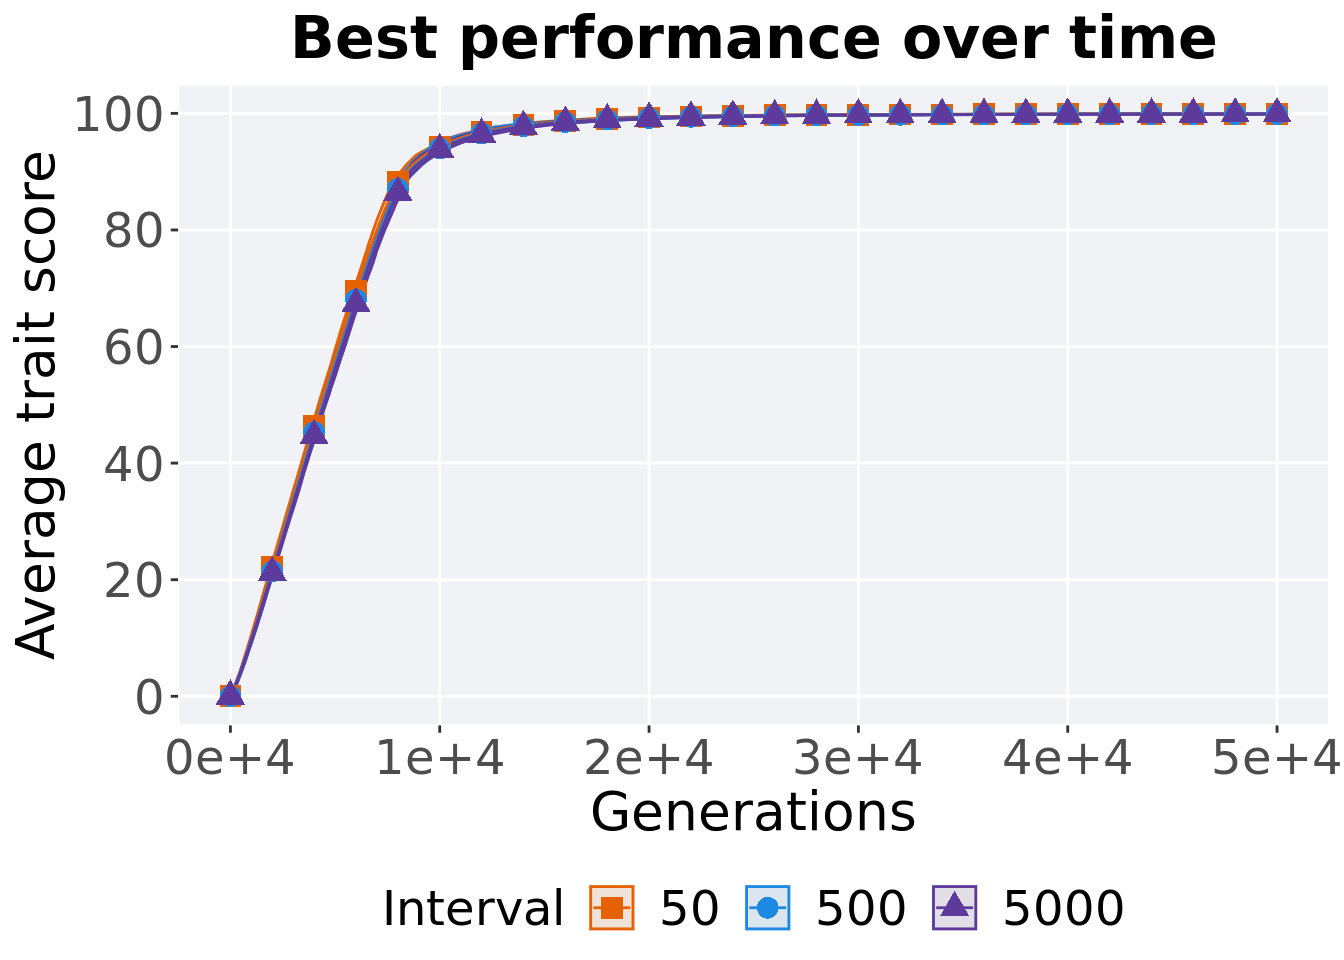
\includegraphics{demo_files/figure-latex/int-tru-ord-perf-1.pdf}

\hypertarget{generation-satisfactory-solution-found-3}{%
\subsection{Generation satisfactory solution found}\label{generation-satisfactory-solution-found-3}}

First generation a satisfactory solution is found throughout the 50,000 generations.

\begin{Shaded}
\begin{Highlighting}[]
\KeywordTok{filter}\NormalTok{(df_ssf, }\StringTok{`}\DataTypeTok{Selection}\CharTok{\textbackslash{}n}\DataTypeTok{Scheme}\StringTok{`} \OperatorTok{==}\StringTok{ 'TRUNCATION'}\NormalTok{) }\OperatorTok
\StringTok{  }\KeywordTok{ggplot}\NormalTok{(., }\KeywordTok{aes}\NormalTok{(}\DataTypeTok{x =}\NormalTok{ Interval, }\DataTypeTok{y =}\NormalTok{ Generations, }\DataTypeTok{color =}\NormalTok{ Interval, }\DataTypeTok{fill =}\NormalTok{ Interval, }\DataTypeTok{shape =}\NormalTok{ Interval)) }\OperatorTok{+}
\StringTok{  }\KeywordTok{geom_flat_violin}\NormalTok{(}\DataTypeTok{position =} \KeywordTok{position_nudge}\NormalTok{(}\DataTypeTok{x =} \FloatTok{.09}\NormalTok{, }\DataTypeTok{y =} \DecValTok{0}\NormalTok{), }\DataTypeTok{scale =} \StringTok{'width'}\NormalTok{, }\DataTypeTok{alpha =} \FloatTok{0.2}\NormalTok{, }\DataTypeTok{width =} \FloatTok{1.5}\NormalTok{) }\OperatorTok{+}
\StringTok{  }\KeywordTok{geom_boxplot}\NormalTok{(}\DataTypeTok{color =} \StringTok{'black'}\NormalTok{, }\DataTypeTok{width =} \FloatTok{.07}\NormalTok{, }\DataTypeTok{outlier.shape =} \OtherTok{NA}\NormalTok{, }\DataTypeTok{alpha =} \FloatTok{0.0}\NormalTok{, }\DataTypeTok{size =} \FloatTok{1.0}\NormalTok{, }\DataTypeTok{position =} \KeywordTok{position_nudge}\NormalTok{(}\DataTypeTok{x =} \FloatTok{.15}\NormalTok{, }\DataTypeTok{y =} \DecValTok{0}\NormalTok{)) }\OperatorTok{+}
\StringTok{  }\KeywordTok{geom_point}\NormalTok{(}\DataTypeTok{position =} \KeywordTok{position_jitter}\NormalTok{(}\DataTypeTok{width =} \FloatTok{.02}\NormalTok{), }\DataTypeTok{size =} \FloatTok{3.0}\NormalTok{, }\DataTypeTok{alpha =} \FloatTok{1.0}\NormalTok{) }\OperatorTok{+}
\StringTok{  }\KeywordTok{scale_shape_manual}\NormalTok{(}\DataTypeTok{values=}\NormalTok{SHAPE)}\OperatorTok{+}
\StringTok{  }\KeywordTok{scale_y_continuous}\NormalTok{(}
    \DataTypeTok{name=}\StringTok{"Generations"}
\NormalTok{  ) }\OperatorTok{+}
\StringTok{  }\KeywordTok{scale_x_discrete}\NormalTok{(}
    \DataTypeTok{name=}\StringTok{"Interval"}
\NormalTok{  ) }\OperatorTok{+}
\StringTok{  }\KeywordTok{scale_colour_manual}\NormalTok{(}\DataTypeTok{values =}\NormalTok{ cb_palette_mi) }\OperatorTok{+}
\StringTok{  }\KeywordTok{scale_fill_manual}\NormalTok{(}\DataTypeTok{values =}\NormalTok{ cb_palette_mi) }\OperatorTok{+}
\StringTok{  }\NormalTok{p_theme}
\end{Highlighting}
\end{Shaded}

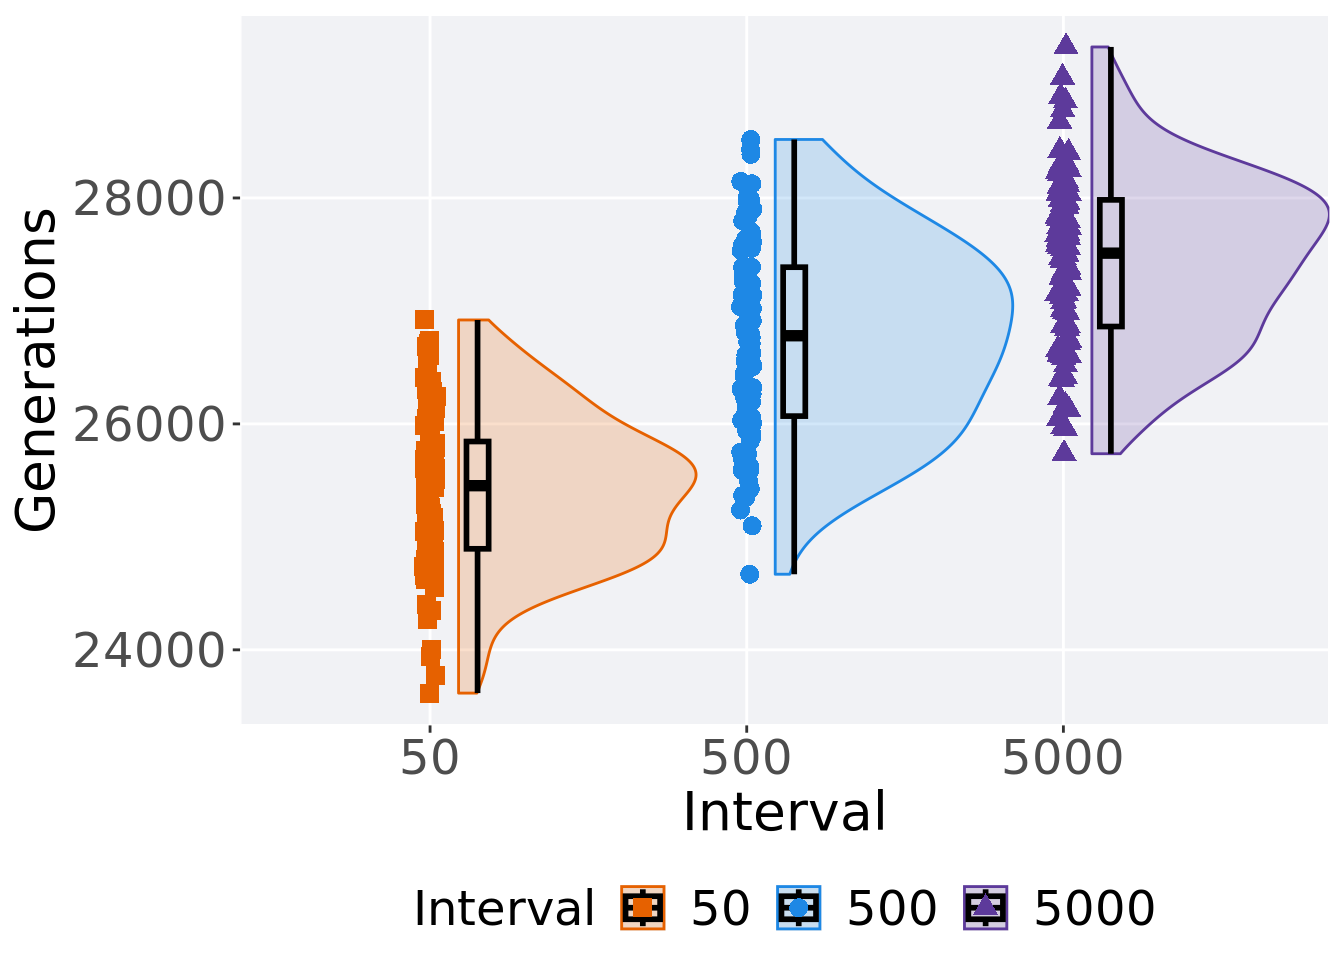
\includegraphics{demo_files/figure-latex/int-tru-ord-ssf-1.pdf}

\hypertarget{stats-3}{%
\subsection{Stats}\label{stats-3}}

Summary statistics for the first generation a satisfactory solution is found.

\begin{Shaded}
\begin{Highlighting}[]
\NormalTok{ssf =}\StringTok{ }\KeywordTok{filter}\NormalTok{(df_ssf, }\StringTok{`}\DataTypeTok{Selection}\CharTok{\textbackslash{}n}\DataTypeTok{Scheme}\StringTok{`} \OperatorTok{==}\StringTok{ 'TRUNCATION'}\NormalTok{)}
\NormalTok{ssf }\OperatorTok
\StringTok{  }\KeywordTok{group_by}\NormalTok{(Interval) }\OperatorTok
\StringTok{  }\NormalTok{dplyr}\OperatorTok{::}\KeywordTok{summarise}\NormalTok{(}
    \DataTypeTok{count =} \KeywordTok{n}\NormalTok{(),}
    \DataTypeTok{na_cnt =} \KeywordTok{sum}\NormalTok{(}\KeywordTok{is.na}\NormalTok{(Generations)),}
    \DataTypeTok{min =} \KeywordTok{min}\NormalTok{(Generations, }\DataTypeTok{na.rm =} \OtherTok{TRUE}\NormalTok{),}
    \DataTypeTok{median =} \KeywordTok{median}\NormalTok{(Generations, }\DataTypeTok{na.rm =} \OtherTok{TRUE}\NormalTok{),}
    \DataTypeTok{mean =} \KeywordTok{mean}\NormalTok{(Generations, }\DataTypeTok{na.rm =} \OtherTok{TRUE}\NormalTok{),}
    \DataTypeTok{max =} \KeywordTok{max}\NormalTok{(Generations, }\DataTypeTok{na.rm =} \OtherTok{TRUE}\NormalTok{),}
    \DataTypeTok{IQR =} \KeywordTok{IQR}\NormalTok{(Generations, }\DataTypeTok{na.rm =} \OtherTok{TRUE}\NormalTok{)}
\NormalTok{  )}
\end{Highlighting}
\end{Shaded}

\begin{verbatim}
## # A tibble: 3 x 8
##   Interval count na_cnt   min median   mean   max   IQR
##   <fct>    <int>  <int> <int>  <dbl>  <dbl> <int> <dbl>
## 1 50         100      0 23617 25453  25405. 26920  950 
## 2 500        100      0 24669 26780. 26767. 28518 1318.
## 3 5000       100      0 25736 27512. 27446. 29337 1121.
\end{verbatim}

Kruskal--Wallis test provides evidence of difference among selection schemes.

\begin{Shaded}
\begin{Highlighting}[]
\KeywordTok{kruskal.test}\NormalTok{(Generations }\OperatorTok{~}\StringTok{ }\NormalTok{Interval, }\DataTypeTok{data =}\NormalTok{ ssf)}
\end{Highlighting}
\end{Shaded}

\begin{verbatim}
## 
##  Kruskal-Wallis rank sum test
## 
## data:  Generations by Interval
## Kruskal-Wallis chi-squared = 168.14, df = 2, p-value < 2.2e-16
\end{verbatim}

Results for post-hoc Wilcoxon rank-sum test with a Bonferroni correction.

\begin{Shaded}
\begin{Highlighting}[]
\KeywordTok{pairwise.wilcox.test}\NormalTok{(}\DataTypeTok{x =}\NormalTok{ ssf}\OperatorTok{$}\NormalTok{Generations, }\DataTypeTok{g =}\NormalTok{ ssf}\OperatorTok{$}\NormalTok{Interval, }\DataTypeTok{p.adjust.method =} \StringTok{"bonferroni"}\NormalTok{,}
                     \DataTypeTok{paired =} \OtherTok{FALSE}\NormalTok{, }\DataTypeTok{conf.int =} \OtherTok{FALSE}\NormalTok{, }\DataTypeTok{alternative =} \StringTok{'g'}\NormalTok{)}
\end{Highlighting}
\end{Shaded}

\begin{verbatim}
## 
##  Pairwise comparisons using Wilcoxon rank sum test with continuity correction 
## 
## data:  ssf$Generations and ssf$Interval 
## 
##      50      500    
## 500  < 2e-16 -      
## 5000 < 2e-16 1.8e-07
## 
## P value adjustment method: bonferroni
\end{verbatim}

\hypertarget{tournament-selection-1}{%
\section{Tournament selection}\label{tournament-selection-1}}

Here we analyze how the different migration intervals affect tournament selection on the exploitation rate diagnostic.

\hypertarget{performance-over-time-4}{%
\subsection{Performance over time}\label{performance-over-time-4}}

\begin{Shaded}
\begin{Highlighting}[]
\NormalTok{lines =}\StringTok{ }\KeywordTok{filter}\NormalTok{(df_ot, }\StringTok{`}\DataTypeTok{Selection}\CharTok{\textbackslash{}n}\DataTypeTok{Scheme}\StringTok{`} \OperatorTok{==}\StringTok{ 'TOURNAMENT'}\NormalTok{) }\OperatorTok
\StringTok{  }\KeywordTok{group_by}\NormalTok{(Interval, Generations) }\OperatorTok
\StringTok{  }\NormalTok{dplyr}\OperatorTok{::}\KeywordTok{summarise}\NormalTok{(}
    \DataTypeTok{min =} \KeywordTok{min}\NormalTok{(pop_fit_max) }\OperatorTok{/}\StringTok{ }\NormalTok{DIMENSIONALITY,}
    \DataTypeTok{mean =} \KeywordTok{mean}\NormalTok{(pop_fit_max) }\OperatorTok{/}\StringTok{ }\NormalTok{DIMENSIONALITY,}
    \DataTypeTok{max =} \KeywordTok{max}\NormalTok{(pop_fit_max) }\OperatorTok{/}\StringTok{ }\NormalTok{DIMENSIONALITY}
\NormalTok{  )}
\KeywordTok{ggplot}\NormalTok{(lines, }\KeywordTok{aes}\NormalTok{(}\DataTypeTok{x=}\NormalTok{Generations, }\DataTypeTok{y=}\NormalTok{mean, }\DataTypeTok{group =}\NormalTok{ Interval, }\DataTypeTok{fill =}\NormalTok{ Interval, }\DataTypeTok{color =}\NormalTok{ Interval, }\DataTypeTok{shape =}\NormalTok{ Interval)) }\OperatorTok{+}
\StringTok{  }\KeywordTok{geom_ribbon}\NormalTok{(}\KeywordTok{aes}\NormalTok{(}\DataTypeTok{ymin =}\NormalTok{ min, }\DataTypeTok{ymax =}\NormalTok{ max), }\DataTypeTok{alpha =} \FloatTok{0.1}\NormalTok{) }\OperatorTok{+}
\StringTok{  }\KeywordTok{geom_line}\NormalTok{(}\DataTypeTok{size =} \FloatTok{0.5}\NormalTok{) }\OperatorTok{+}
\StringTok{  }\KeywordTok{geom_point}\NormalTok{(}\DataTypeTok{data =} \KeywordTok{filter}\NormalTok{(lines, Generations }\OperatorTok\StringTok{ }\DecValTok{2000} \OperatorTok{==}\StringTok{ }\DecValTok{0}\NormalTok{), }\DataTypeTok{size =} \FloatTok{2.5}\NormalTok{, }\DataTypeTok{stroke =} \FloatTok{2.0}\NormalTok{, }\DataTypeTok{alpha =} \FloatTok{1.0}\NormalTok{) }\OperatorTok{+}
\StringTok{  }\KeywordTok{scale_y_continuous}\NormalTok{(}
    \DataTypeTok{name=}\StringTok{"Average trait score"}\NormalTok{,}
    \DataTypeTok{limits=}\KeywordTok{c}\NormalTok{(}\DecValTok{0}\NormalTok{, }\DecValTok{100}\NormalTok{),}
    \DataTypeTok{breaks=}\KeywordTok{seq}\NormalTok{(}\DecValTok{0}\NormalTok{,}\DecValTok{100}\NormalTok{, }\DecValTok{20}\NormalTok{),}
    \DataTypeTok{labels=}\KeywordTok{c}\NormalTok{(}\StringTok{"0"}\NormalTok{, }\StringTok{"20"}\NormalTok{, }\StringTok{"40"}\NormalTok{, }\StringTok{"60"}\NormalTok{, }\StringTok{"80"}\NormalTok{, }\StringTok{"100"}\NormalTok{)}
\NormalTok{  ) }\OperatorTok{+}
\StringTok{  }\KeywordTok{scale_x_continuous}\NormalTok{(}
    \DataTypeTok{name=}\StringTok{"Generations"}\NormalTok{,}
    \DataTypeTok{limits=}\KeywordTok{c}\NormalTok{(}\DecValTok{0}\NormalTok{, }\DecValTok{50000}\NormalTok{),}
    \DataTypeTok{breaks=}\KeywordTok{c}\NormalTok{(}\DecValTok{0}\NormalTok{, }\DecValTok{10000}\NormalTok{, }\DecValTok{20000}\NormalTok{, }\DecValTok{30000}\NormalTok{, }\DecValTok{40000}\NormalTok{, }\DecValTok{50000}\NormalTok{),}
    \DataTypeTok{labels=}\KeywordTok{c}\NormalTok{(}\StringTok{"0e+4"}\NormalTok{, }\StringTok{"1e+4"}\NormalTok{, }\StringTok{"2e+4"}\NormalTok{, }\StringTok{"3e+4"}\NormalTok{, }\StringTok{"4e+4"}\NormalTok{, }\StringTok{"5e+4"}\NormalTok{)}

\NormalTok{  ) }\OperatorTok{+}
\StringTok{  }\KeywordTok{scale_shape_manual}\NormalTok{(}\DataTypeTok{values=}\NormalTok{SHAPE)}\OperatorTok{+}
\StringTok{  }\KeywordTok{scale_colour_manual}\NormalTok{(}\DataTypeTok{values =}\NormalTok{ cb_palette_mi) }\OperatorTok{+}
\StringTok{  }\KeywordTok{scale_fill_manual}\NormalTok{(}\DataTypeTok{values =}\NormalTok{ cb_palette_mi) }\OperatorTok{+}
\StringTok{  }\KeywordTok{ggtitle}\NormalTok{(}\StringTok{"Best performance over time"}\NormalTok{) }\OperatorTok{+}
\StringTok{  }\NormalTok{p_theme}
\end{Highlighting}
\end{Shaded}

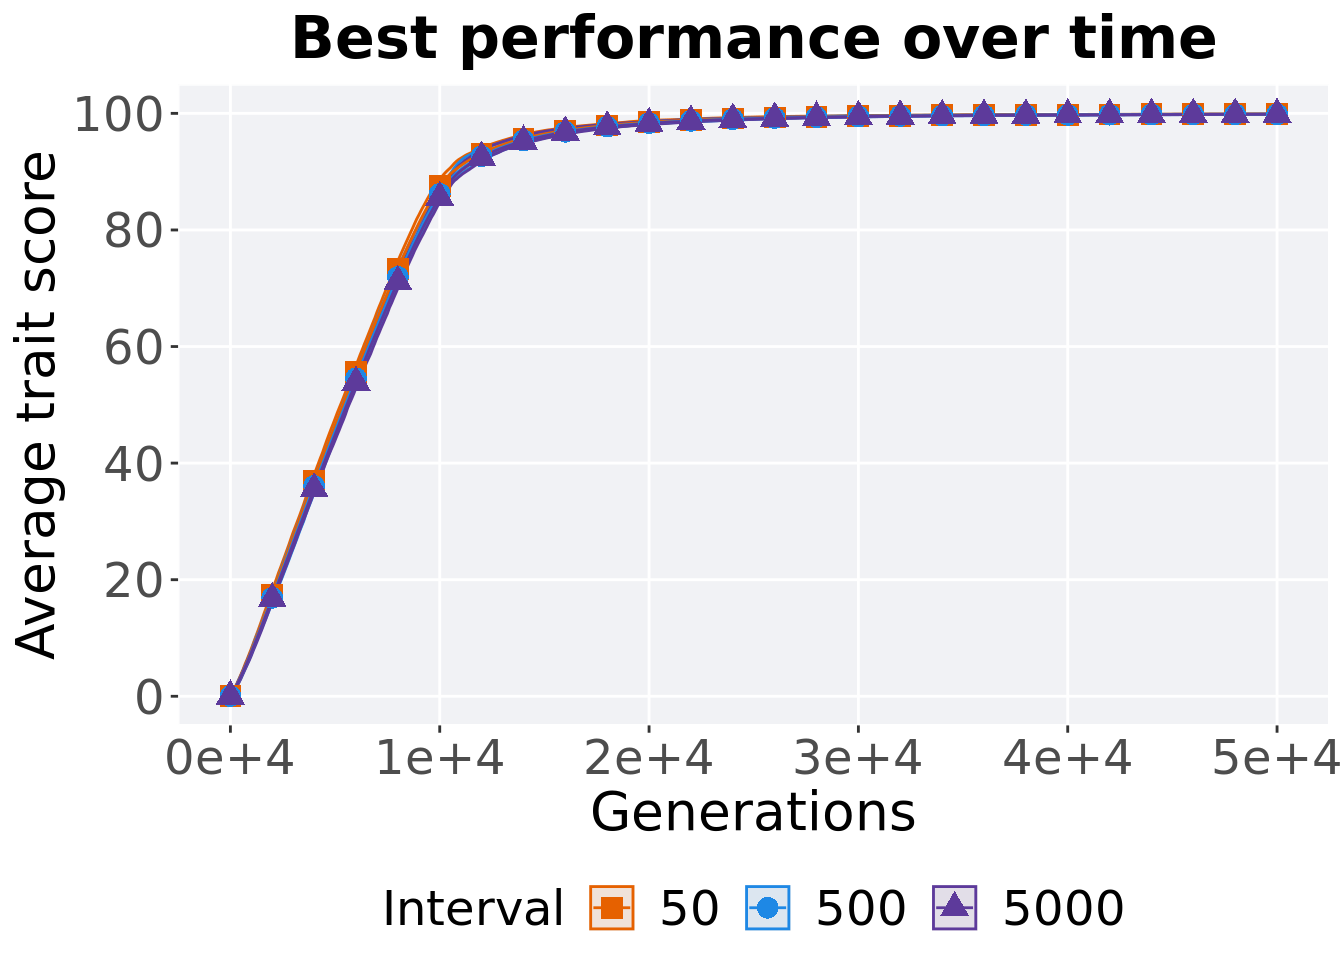
\includegraphics{demo_files/figure-latex/int-tor-ord-perf-1.pdf}

\hypertarget{generation-satisfactory-solution-found-4}{%
\subsection{Generation satisfactory solution found}\label{generation-satisfactory-solution-found-4}}

First generation a satisfactory solution is found throughout the 50,000 generations.

\begin{Shaded}
\begin{Highlighting}[]
\KeywordTok{filter}\NormalTok{(df_ssf, }\StringTok{`}\DataTypeTok{Selection}\CharTok{\textbackslash{}n}\DataTypeTok{Scheme}\StringTok{`} \OperatorTok{==}\StringTok{ 'TOURNAMENT'}\NormalTok{) }\OperatorTok
\StringTok{  }\KeywordTok{ggplot}\NormalTok{(., }\KeywordTok{aes}\NormalTok{(}\DataTypeTok{x =}\NormalTok{ Interval, }\DataTypeTok{y =}\NormalTok{ Generations, }\DataTypeTok{color =}\NormalTok{ Interval, }\DataTypeTok{fill =}\NormalTok{ Interval, }\DataTypeTok{shape =}\NormalTok{ Interval)) }\OperatorTok{+}
\StringTok{  }\KeywordTok{geom_flat_violin}\NormalTok{(}\DataTypeTok{position =} \KeywordTok{position_nudge}\NormalTok{(}\DataTypeTok{x =} \FloatTok{.09}\NormalTok{, }\DataTypeTok{y =} \DecValTok{0}\NormalTok{), }\DataTypeTok{scale =} \StringTok{'width'}\NormalTok{, }\DataTypeTok{alpha =} \FloatTok{0.2}\NormalTok{, }\DataTypeTok{width =} \FloatTok{1.5}\NormalTok{) }\OperatorTok{+}
\StringTok{  }\KeywordTok{geom_boxplot}\NormalTok{(}\DataTypeTok{color =} \StringTok{'black'}\NormalTok{, }\DataTypeTok{width =} \FloatTok{.07}\NormalTok{, }\DataTypeTok{outlier.shape =} \OtherTok{NA}\NormalTok{, }\DataTypeTok{alpha =} \FloatTok{0.0}\NormalTok{, }\DataTypeTok{size =} \FloatTok{1.0}\NormalTok{, }\DataTypeTok{position =} \KeywordTok{position_nudge}\NormalTok{(}\DataTypeTok{x =} \FloatTok{.15}\NormalTok{, }\DataTypeTok{y =} \DecValTok{0}\NormalTok{)) }\OperatorTok{+}
\StringTok{  }\KeywordTok{geom_point}\NormalTok{(}\DataTypeTok{position =} \KeywordTok{position_jitter}\NormalTok{(}\DataTypeTok{width =} \FloatTok{.02}\NormalTok{), }\DataTypeTok{size =} \FloatTok{3.0}\NormalTok{, }\DataTypeTok{alpha =} \FloatTok{1.0}\NormalTok{) }\OperatorTok{+}
\StringTok{  }\KeywordTok{scale_shape_manual}\NormalTok{(}\DataTypeTok{values=}\NormalTok{SHAPE)}\OperatorTok{+}
\StringTok{  }\KeywordTok{scale_y_continuous}\NormalTok{(}
    \DataTypeTok{name=}\StringTok{"Generations"}
\NormalTok{  ) }\OperatorTok{+}
\StringTok{  }\KeywordTok{scale_x_discrete}\NormalTok{(}
    \DataTypeTok{name=}\StringTok{"Interval"}
\NormalTok{  ) }\OperatorTok{+}
\StringTok{  }\KeywordTok{scale_colour_manual}\NormalTok{(}\DataTypeTok{values =}\NormalTok{ cb_palette_mi) }\OperatorTok{+}
\StringTok{  }\KeywordTok{scale_fill_manual}\NormalTok{(}\DataTypeTok{values =}\NormalTok{ cb_palette_mi) }\OperatorTok{+}
\StringTok{  }\NormalTok{p_theme}
\end{Highlighting}
\end{Shaded}

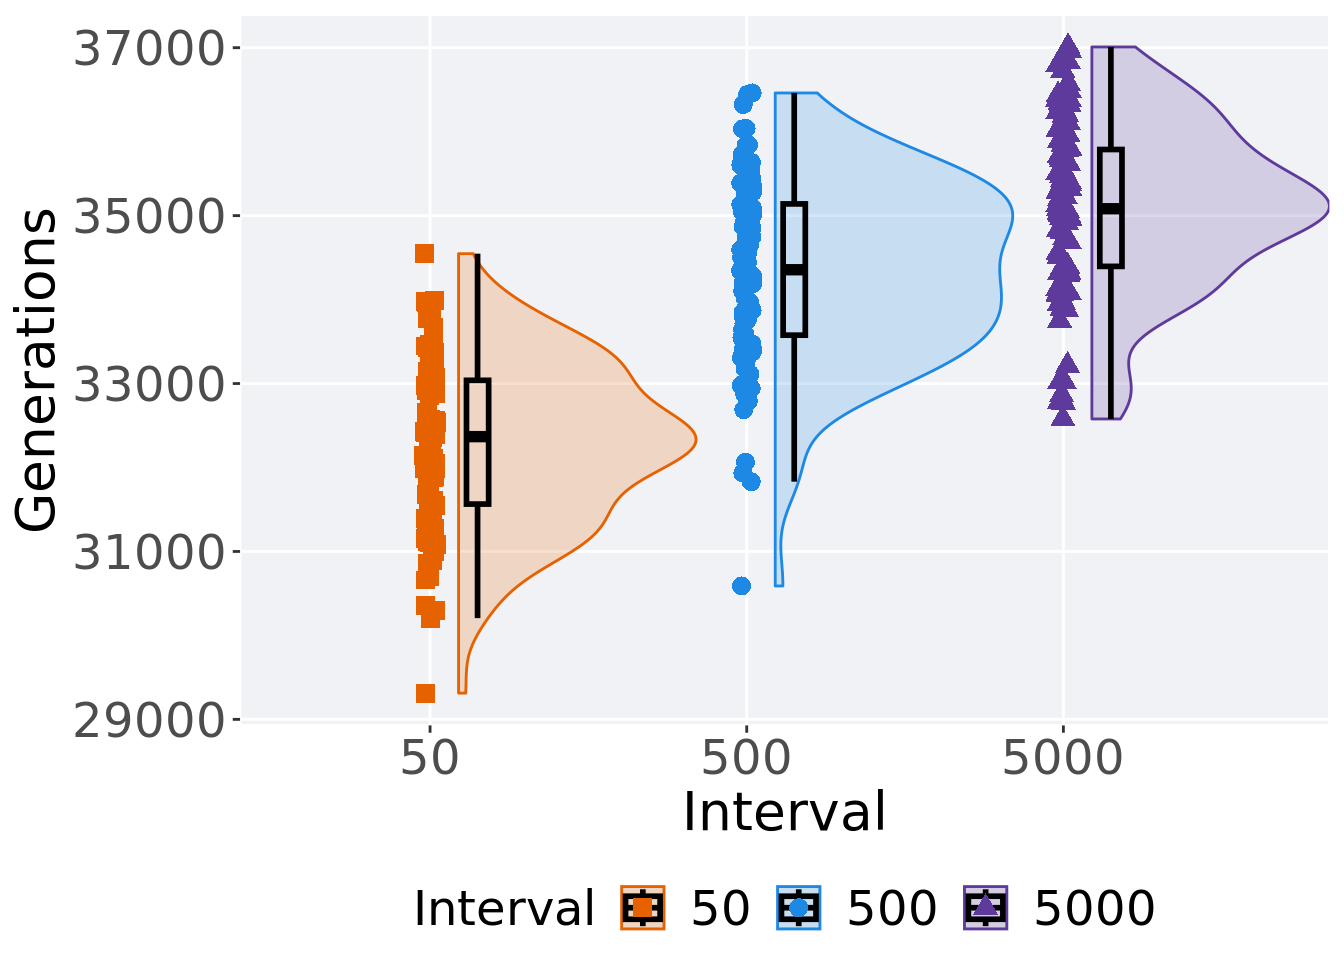
\includegraphics{demo_files/figure-latex/int-tor-ord-ssf-1.pdf}

\hypertarget{stats-4}{%
\subsection{Stats}\label{stats-4}}

Summary statistics for the first generation a satisfactory solution is found.

\begin{Shaded}
\begin{Highlighting}[]
\NormalTok{ssf =}\StringTok{ }\KeywordTok{filter}\NormalTok{(df_ssf, }\StringTok{`}\DataTypeTok{Selection}\CharTok{\textbackslash{}n}\DataTypeTok{Scheme}\StringTok{`} \OperatorTok{==}\StringTok{ 'TOURNAMENT'}\NormalTok{)}
\NormalTok{ssf }\OperatorTok
\StringTok{  }\KeywordTok{group_by}\NormalTok{(Interval) }\OperatorTok
\StringTok{  }\NormalTok{dplyr}\OperatorTok{::}\KeywordTok{summarise}\NormalTok{(}
    \DataTypeTok{count =} \KeywordTok{n}\NormalTok{(),}
    \DataTypeTok{na_cnt =} \KeywordTok{sum}\NormalTok{(}\KeywordTok{is.na}\NormalTok{(Generations)),}
    \DataTypeTok{min =} \KeywordTok{min}\NormalTok{(Generations, }\DataTypeTok{na.rm =} \OtherTok{TRUE}\NormalTok{),}
    \DataTypeTok{median =} \KeywordTok{median}\NormalTok{(Generations, }\DataTypeTok{na.rm =} \OtherTok{TRUE}\NormalTok{),}
    \DataTypeTok{mean =} \KeywordTok{mean}\NormalTok{(Generations, }\DataTypeTok{na.rm =} \OtherTok{TRUE}\NormalTok{),}
    \DataTypeTok{max =} \KeywordTok{max}\NormalTok{(Generations, }\DataTypeTok{na.rm =} \OtherTok{TRUE}\NormalTok{),}
    \DataTypeTok{IQR =} \KeywordTok{IQR}\NormalTok{(Generations, }\DataTypeTok{na.rm =} \OtherTok{TRUE}\NormalTok{)}
\NormalTok{  )}
\end{Highlighting}
\end{Shaded}

\begin{verbatim}
## # A tibble: 3 x 8
##   Interval count na_cnt   min median   mean   max   IQR
##   <fct>    <int>  <int> <int>  <dbl>  <dbl> <int> <dbl>
## 1 50         100      0 29313 32368. 32281. 34547 1474 
## 2 500        100      0 30589 34356. 34349. 36461 1564.
## 3 5000       100      0 32578 35082  35088. 37009 1392
\end{verbatim}

Kruskal--Wallis test provides evidence of difference among selection schemes.

\begin{Shaded}
\begin{Highlighting}[]
\KeywordTok{kruskal.test}\NormalTok{(Generations }\OperatorTok{~}\StringTok{ }\NormalTok{Interval, }\DataTypeTok{data =}\NormalTok{ ssf)}
\end{Highlighting}
\end{Shaded}

\begin{verbatim}
## 
##  Kruskal-Wallis rank sum test
## 
## data:  Generations by Interval
## Kruskal-Wallis chi-squared = 172.97, df = 2, p-value < 2.2e-16
\end{verbatim}

Results for post-hoc Wilcoxon rank-sum test with a Bonferroni correction.

\begin{Shaded}
\begin{Highlighting}[]
\KeywordTok{pairwise.wilcox.test}\NormalTok{(}\DataTypeTok{x =}\NormalTok{ ssf}\OperatorTok{$}\NormalTok{Generations, }\DataTypeTok{g =}\NormalTok{ ssf}\OperatorTok{$}\NormalTok{Interval, }\DataTypeTok{p.adjust.method =} \StringTok{"bonferroni"}\NormalTok{,}
                     \DataTypeTok{paired =} \OtherTok{FALSE}\NormalTok{, }\DataTypeTok{conf.int =} \OtherTok{FALSE}\NormalTok{, }\DataTypeTok{alternative =} \StringTok{'g'}\NormalTok{)}
\end{Highlighting}
\end{Shaded}

\begin{verbatim}
## 
##  Pairwise comparisons using Wilcoxon rank sum test with continuity correction 
## 
## data:  ssf$Generations and ssf$Interval 
## 
##      50      500    
## 500  < 2e-16 -      
## 5000 < 2e-16 5.9e-06
## 
## P value adjustment method: bonferroni
\end{verbatim}

\hypertarget{lexicase-selection-1}{%
\section{Lexicase selection}\label{lexicase-selection-1}}

Here we analyze how the different migration intervals affect tournament selection on the exploitation rate diagnostic.

\hypertarget{performance-over-time-5}{%
\subsection{Performance over time}\label{performance-over-time-5}}

\begin{Shaded}
\begin{Highlighting}[]
\NormalTok{lines =}\StringTok{ }\KeywordTok{filter}\NormalTok{(df_ot, }\StringTok{`}\DataTypeTok{Selection}\CharTok{\textbackslash{}n}\DataTypeTok{Scheme}\StringTok{`} \OperatorTok{==}\StringTok{ 'LEXICASE'}\NormalTok{) }\OperatorTok
\StringTok{  }\KeywordTok{group_by}\NormalTok{(Interval, Generations) }\OperatorTok
\StringTok{  }\NormalTok{dplyr}\OperatorTok{::}\KeywordTok{summarise}\NormalTok{(}
    \DataTypeTok{min =} \KeywordTok{min}\NormalTok{(pop_fit_max) }\OperatorTok{/}\StringTok{ }\NormalTok{DIMENSIONALITY,}
    \DataTypeTok{mean =} \KeywordTok{mean}\NormalTok{(pop_fit_max) }\OperatorTok{/}\StringTok{ }\NormalTok{DIMENSIONALITY,}
    \DataTypeTok{max =} \KeywordTok{max}\NormalTok{(pop_fit_max) }\OperatorTok{/}\StringTok{ }\NormalTok{DIMENSIONALITY}
\NormalTok{  )}
\KeywordTok{ggplot}\NormalTok{(lines, }\KeywordTok{aes}\NormalTok{(}\DataTypeTok{x=}\NormalTok{Generations, }\DataTypeTok{y=}\NormalTok{mean, }\DataTypeTok{group =}\NormalTok{ Interval, }\DataTypeTok{fill =}\NormalTok{ Interval, }\DataTypeTok{color =}\NormalTok{ Interval, }\DataTypeTok{shape =}\NormalTok{ Interval)) }\OperatorTok{+}
\StringTok{  }\KeywordTok{geom_ribbon}\NormalTok{(}\KeywordTok{aes}\NormalTok{(}\DataTypeTok{ymin =}\NormalTok{ min, }\DataTypeTok{ymax =}\NormalTok{ max), }\DataTypeTok{alpha =} \FloatTok{0.1}\NormalTok{) }\OperatorTok{+}
\StringTok{  }\KeywordTok{geom_line}\NormalTok{(}\DataTypeTok{size =} \FloatTok{0.5}\NormalTok{) }\OperatorTok{+}
\StringTok{  }\KeywordTok{geom_point}\NormalTok{(}\DataTypeTok{data =} \KeywordTok{filter}\NormalTok{(lines, Generations }\OperatorTok\StringTok{ }\DecValTok{2000} \OperatorTok{==}\StringTok{ }\DecValTok{0}\NormalTok{), }\DataTypeTok{size =} \FloatTok{2.5}\NormalTok{, }\DataTypeTok{stroke =} \FloatTok{2.0}\NormalTok{, }\DataTypeTok{alpha =} \FloatTok{1.0}\NormalTok{) }\OperatorTok{+}
\StringTok{  }\KeywordTok{scale_y_continuous}\NormalTok{(}
    \DataTypeTok{name=}\StringTok{"Average trait score"}\NormalTok{,}
    \DataTypeTok{limits=}\KeywordTok{c}\NormalTok{(}\DecValTok{0}\NormalTok{, }\DecValTok{100}\NormalTok{),}
    \DataTypeTok{breaks=}\KeywordTok{seq}\NormalTok{(}\DecValTok{0}\NormalTok{,}\DecValTok{100}\NormalTok{, }\DecValTok{20}\NormalTok{),}
    \DataTypeTok{labels=}\KeywordTok{c}\NormalTok{(}\StringTok{"0"}\NormalTok{, }\StringTok{"20"}\NormalTok{, }\StringTok{"40"}\NormalTok{, }\StringTok{"60"}\NormalTok{, }\StringTok{"80"}\NormalTok{, }\StringTok{"100"}\NormalTok{)}
\NormalTok{  ) }\OperatorTok{+}
\StringTok{  }\KeywordTok{scale_x_continuous}\NormalTok{(}
    \DataTypeTok{name=}\StringTok{"Generations"}\NormalTok{,}
    \DataTypeTok{limits=}\KeywordTok{c}\NormalTok{(}\DecValTok{0}\NormalTok{, }\DecValTok{50000}\NormalTok{),}
    \DataTypeTok{breaks=}\KeywordTok{c}\NormalTok{(}\DecValTok{0}\NormalTok{, }\DecValTok{10000}\NormalTok{, }\DecValTok{20000}\NormalTok{, }\DecValTok{30000}\NormalTok{, }\DecValTok{40000}\NormalTok{, }\DecValTok{50000}\NormalTok{),}
    \DataTypeTok{labels=}\KeywordTok{c}\NormalTok{(}\StringTok{"0e+4"}\NormalTok{, }\StringTok{"1e+4"}\NormalTok{, }\StringTok{"2e+4"}\NormalTok{, }\StringTok{"3e+4"}\NormalTok{, }\StringTok{"4e+4"}\NormalTok{, }\StringTok{"5e+4"}\NormalTok{)}

\NormalTok{  ) }\OperatorTok{+}
\StringTok{  }\KeywordTok{scale_shape_manual}\NormalTok{(}\DataTypeTok{values=}\NormalTok{SHAPE)}\OperatorTok{+}
\StringTok{  }\KeywordTok{scale_colour_manual}\NormalTok{(}\DataTypeTok{values =}\NormalTok{ cb_palette_mi) }\OperatorTok{+}
\StringTok{  }\KeywordTok{scale_fill_manual}\NormalTok{(}\DataTypeTok{values =}\NormalTok{ cb_palette_mi) }\OperatorTok{+}
\StringTok{  }\KeywordTok{ggtitle}\NormalTok{(}\StringTok{"Best performance over time"}\NormalTok{) }\OperatorTok{+}
\StringTok{  }\NormalTok{p_theme}
\end{Highlighting}
\end{Shaded}

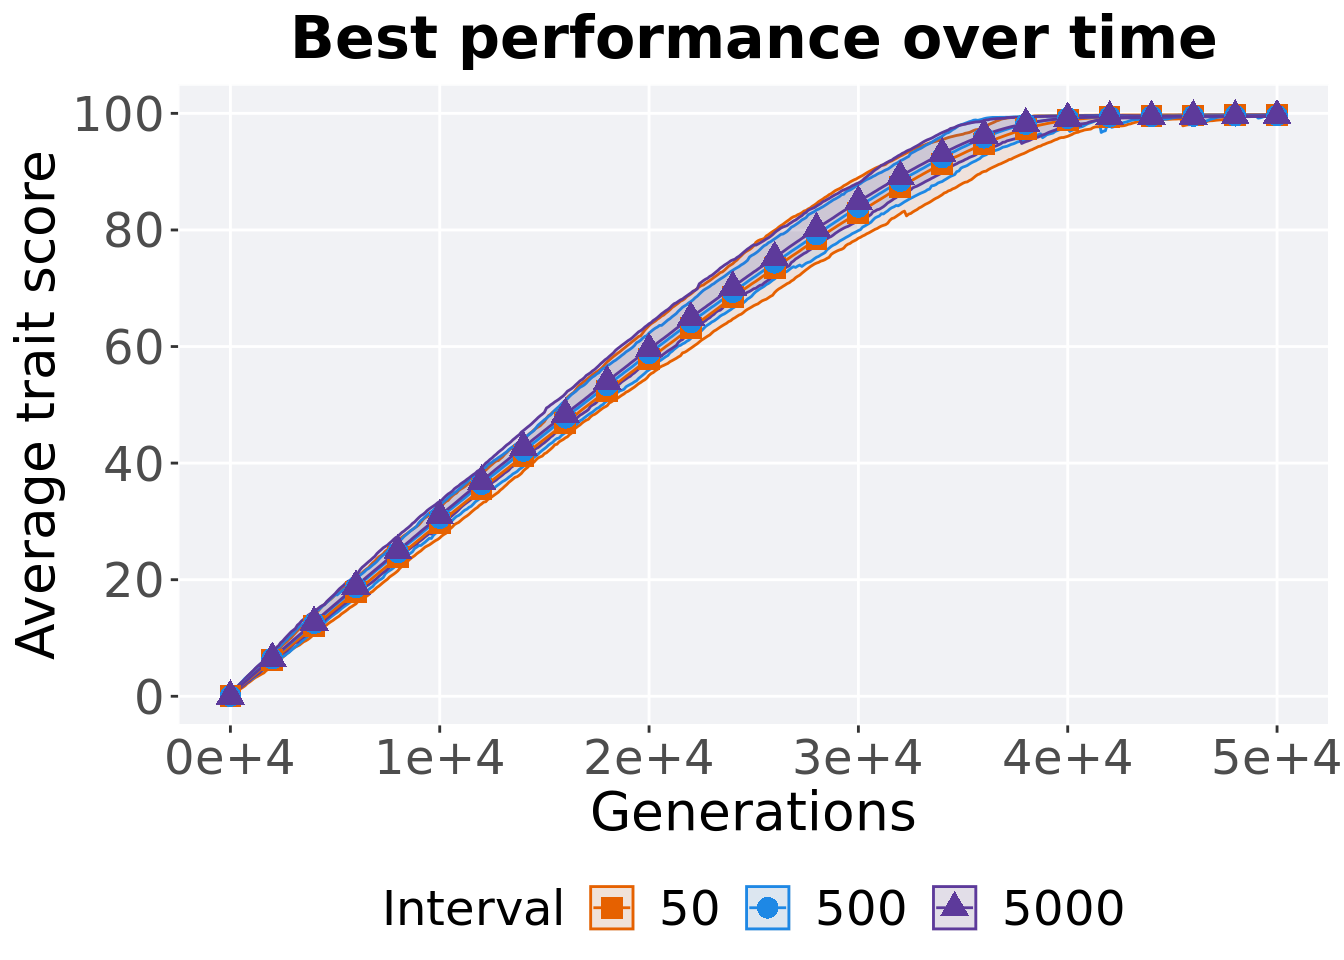
\includegraphics{demo_files/figure-latex/int-lex-ord-perf-1.pdf}

\hypertarget{generation-satisfactory-solution-found-5}{%
\subsection{Generation satisfactory solution found}\label{generation-satisfactory-solution-found-5}}

First generation a satisfactory solution is found throughout the 50,000 generations.

\begin{Shaded}
\begin{Highlighting}[]
\KeywordTok{filter}\NormalTok{(df_ssf, }\StringTok{`}\DataTypeTok{Selection}\CharTok{\textbackslash{}n}\DataTypeTok{Scheme}\StringTok{`} \OperatorTok{==}\StringTok{ 'LEXICASE'}\NormalTok{) }\OperatorTok
\StringTok{  }\KeywordTok{ggplot}\NormalTok{(., }\KeywordTok{aes}\NormalTok{(}\DataTypeTok{x =}\NormalTok{ Interval, }\DataTypeTok{y =}\NormalTok{ Generations, }\DataTypeTok{color =}\NormalTok{ Interval, }\DataTypeTok{fill =}\NormalTok{ Interval, }\DataTypeTok{shape =}\NormalTok{ Interval)) }\OperatorTok{+}
\StringTok{  }\KeywordTok{geom_flat_violin}\NormalTok{(}\DataTypeTok{position =} \KeywordTok{position_nudge}\NormalTok{(}\DataTypeTok{x =} \FloatTok{.09}\NormalTok{, }\DataTypeTok{y =} \DecValTok{0}\NormalTok{), }\DataTypeTok{scale =} \StringTok{'width'}\NormalTok{, }\DataTypeTok{alpha =} \FloatTok{0.2}\NormalTok{, }\DataTypeTok{width =} \FloatTok{1.5}\NormalTok{) }\OperatorTok{+}
\StringTok{  }\KeywordTok{geom_boxplot}\NormalTok{(}\DataTypeTok{color =} \StringTok{'black'}\NormalTok{, }\DataTypeTok{width =} \FloatTok{.07}\NormalTok{, }\DataTypeTok{outlier.shape =} \OtherTok{NA}\NormalTok{, }\DataTypeTok{alpha =} \FloatTok{0.0}\NormalTok{, }\DataTypeTok{size =} \FloatTok{1.0}\NormalTok{, }\DataTypeTok{position =} \KeywordTok{position_nudge}\NormalTok{(}\DataTypeTok{x =} \FloatTok{.15}\NormalTok{, }\DataTypeTok{y =} \DecValTok{0}\NormalTok{)) }\OperatorTok{+}
\StringTok{  }\KeywordTok{geom_point}\NormalTok{(}\DataTypeTok{position =} \KeywordTok{position_jitter}\NormalTok{(}\DataTypeTok{width =} \FloatTok{.02}\NormalTok{), }\DataTypeTok{size =} \FloatTok{3.0}\NormalTok{, }\DataTypeTok{alpha =} \FloatTok{1.0}\NormalTok{) }\OperatorTok{+}
\StringTok{  }\KeywordTok{scale_shape_manual}\NormalTok{(}\DataTypeTok{values=}\NormalTok{SHAPE)}\OperatorTok{+}
\StringTok{  }\KeywordTok{scale_y_continuous}\NormalTok{(}
    \DataTypeTok{name=}\StringTok{"Generations"}
\NormalTok{  ) }\OperatorTok{+}
\StringTok{  }\KeywordTok{scale_x_discrete}\NormalTok{(}
    \DataTypeTok{name=}\StringTok{"Interval"}
\NormalTok{  ) }\OperatorTok{+}
\StringTok{  }\KeywordTok{scale_colour_manual}\NormalTok{(}\DataTypeTok{values =}\NormalTok{ cb_palette_mi) }\OperatorTok{+}
\StringTok{  }\KeywordTok{scale_fill_manual}\NormalTok{(}\DataTypeTok{values =}\NormalTok{ cb_palette_mi) }\OperatorTok{+}
\StringTok{  }\NormalTok{p_theme}
\end{Highlighting}
\end{Shaded}

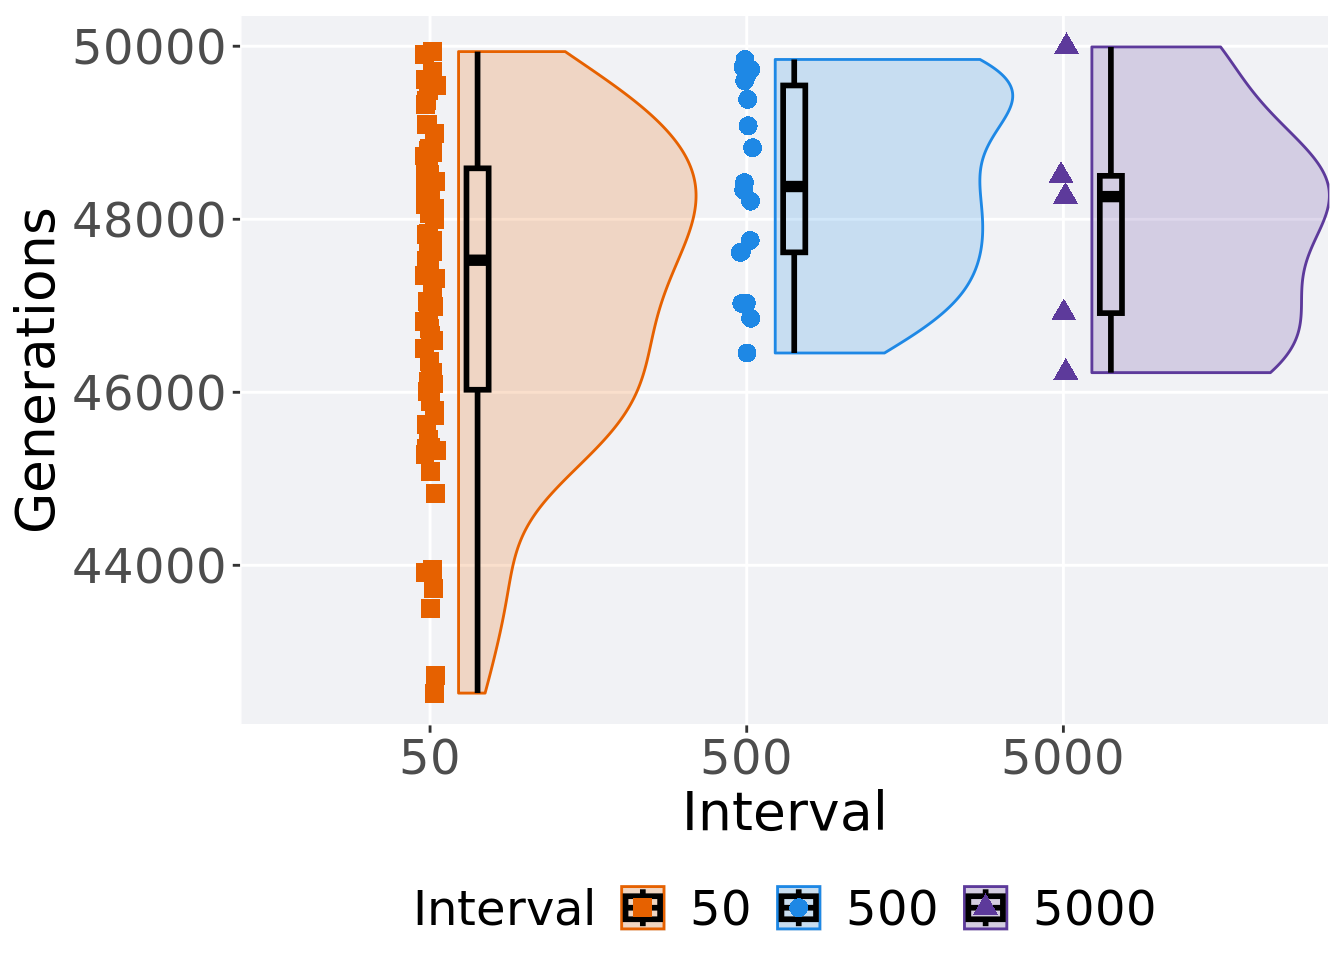
\includegraphics{demo_files/figure-latex/int-lex-ord-ssf-1.pdf}

\hypertarget{stats-5}{%
\subsection{Stats}\label{stats-5}}

Summary statistics for the first generation a satisfactory solution is found.

\begin{Shaded}
\begin{Highlighting}[]
\NormalTok{ssf =}\StringTok{ }\KeywordTok{filter}\NormalTok{(df_ssf, }\StringTok{`}\DataTypeTok{Selection}\CharTok{\textbackslash{}n}\DataTypeTok{Scheme}\StringTok{`} \OperatorTok{==}\StringTok{ 'LEXICASE'}\NormalTok{)}
\NormalTok{ssf }\OperatorTok
\StringTok{  }\KeywordTok{group_by}\NormalTok{(Interval) }\OperatorTok
\StringTok{  }\NormalTok{dplyr}\OperatorTok{::}\KeywordTok{summarise}\NormalTok{(}
    \DataTypeTok{count =} \KeywordTok{n}\NormalTok{(),}
    \DataTypeTok{na_cnt =} \KeywordTok{sum}\NormalTok{(}\KeywordTok{is.na}\NormalTok{(Generations)),}
    \DataTypeTok{min =} \KeywordTok{min}\NormalTok{(Generations, }\DataTypeTok{na.rm =} \OtherTok{TRUE}\NormalTok{),}
    \DataTypeTok{median =} \KeywordTok{median}\NormalTok{(Generations, }\DataTypeTok{na.rm =} \OtherTok{TRUE}\NormalTok{),}
    \DataTypeTok{mean =} \KeywordTok{mean}\NormalTok{(Generations, }\DataTypeTok{na.rm =} \OtherTok{TRUE}\NormalTok{),}
    \DataTypeTok{max =} \KeywordTok{max}\NormalTok{(Generations, }\DataTypeTok{na.rm =} \OtherTok{TRUE}\NormalTok{),}
    \DataTypeTok{IQR =} \KeywordTok{IQR}\NormalTok{(Generations, }\DataTypeTok{na.rm =} \OtherTok{TRUE}\NormalTok{)}
\NormalTok{  )}
\end{Highlighting}
\end{Shaded}

\begin{verbatim}
## # A tibble: 3 x 8
##   Interval count na_cnt   min median   mean   max   IQR
##   <fct>    <int>  <int> <int>  <dbl>  <dbl> <int> <dbl>
## 1 50          70      0 42523 47526. 47195. 49938 2560.
## 2 500         18      0 46454 48378. 48402. 49847 1929 
## 3 5000         5      0 46227 48262  47980. 49992 1587
\end{verbatim}

Kruskal--Wallis test provides evidence of difference among selection schemes.

\begin{Shaded}
\begin{Highlighting}[]
\KeywordTok{kruskal.test}\NormalTok{(Generations }\OperatorTok{~}\StringTok{ }\NormalTok{Interval, }\DataTypeTok{data =}\NormalTok{ ssf)}
\end{Highlighting}
\end{Shaded}

\begin{verbatim}
## 
##  Kruskal-Wallis rank sum test
## 
## data:  Generations by Interval
## Kruskal-Wallis chi-squared = 7.1725, df = 2, p-value = 0.0277
\end{verbatim}

Results for post-hoc Wilcoxon rank-sum test with a Bonferroni correction.

\begin{Shaded}
\begin{Highlighting}[]
\KeywordTok{pairwise.wilcox.test}\NormalTok{(}\DataTypeTok{x =}\NormalTok{ ssf}\OperatorTok{$}\NormalTok{Generations, }\DataTypeTok{g =}\NormalTok{ ssf}\OperatorTok{$}\NormalTok{Interval, }\DataTypeTok{p.adjust.method =} \StringTok{"bonferroni"}\NormalTok{,}
                     \DataTypeTok{paired =} \OtherTok{FALSE}\NormalTok{, }\DataTypeTok{conf.int =} \OtherTok{FALSE}\NormalTok{, }\DataTypeTok{alternative =} \StringTok{'t'}\NormalTok{)}
\end{Highlighting}
\end{Shaded}

\begin{verbatim}
## 
##  Pairwise comparisons using Wilcoxon rank sum test with continuity correction 
## 
## data:  ssf$Generations and ssf$Interval 
## 
##      50    500  
## 500  0.027 -    
## 5000 1.000 1.000
## 
## P value adjustment method: bonferroni
\end{verbatim}

\hypertarget{best-performance-thorughout-run}{%
\subsection{Best performance thorughout run}\label{best-performance-thorughout-run}}

\begin{Shaded}
\begin{Highlighting}[]
\KeywordTok{filter}\NormalTok{(df_best, Diagnostic }\OperatorTok{==}\StringTok{ 'ORDERED_EXPLOITATION'} \OperatorTok{&}\StringTok{ `}\DataTypeTok{Selection}\CharTok{\textbackslash{}n}\DataTypeTok{Scheme}\StringTok{`} \OperatorTok{==}\StringTok{ 'LEXICASE'} \OperatorTok{&}\StringTok{ }\NormalTok{VAR }\OperatorTok{==}\StringTok{ 'pop_fit_max'}\NormalTok{) }\OperatorTok
\StringTok{  }\KeywordTok{ggplot}\NormalTok{(., }\KeywordTok{aes}\NormalTok{(}\DataTypeTok{x =}\NormalTok{ Interval, }\DataTypeTok{y =}\NormalTok{ VAL }\OperatorTok{/}\StringTok{ }\NormalTok{DIMENSIONALITY, }\DataTypeTok{color =}\NormalTok{ Interval, }\DataTypeTok{fill =}\NormalTok{ Interval, }\DataTypeTok{shape =}\NormalTok{ Interval)) }\OperatorTok{+}
\StringTok{  }\KeywordTok{geom_flat_violin}\NormalTok{(}\DataTypeTok{position =} \KeywordTok{position_nudge}\NormalTok{(}\DataTypeTok{x =} \FloatTok{.2}\NormalTok{, }\DataTypeTok{y =} \DecValTok{0}\NormalTok{), }\DataTypeTok{scale =} \StringTok{'width'}\NormalTok{, }\DataTypeTok{alpha =} \FloatTok{0.2}\NormalTok{) }\OperatorTok{+}
\StringTok{  }\KeywordTok{geom_point}\NormalTok{(}\DataTypeTok{position =} \KeywordTok{position_jitter}\NormalTok{(}\DataTypeTok{width =} \FloatTok{.1}\NormalTok{), }\DataTypeTok{size =} \FloatTok{1.5}\NormalTok{, }\DataTypeTok{alpha =} \FloatTok{1.0}\NormalTok{) }\OperatorTok{+}
\StringTok{  }\KeywordTok{geom_boxplot}\NormalTok{(}\DataTypeTok{color =} \StringTok{'black'}\NormalTok{, }\DataTypeTok{width =} \FloatTok{.2}\NormalTok{, }\DataTypeTok{outlier.shape =} \OtherTok{NA}\NormalTok{, }\DataTypeTok{alpha =} \FloatTok{0.0}\NormalTok{) }\OperatorTok{+}
\StringTok{  }\KeywordTok{scale_y_continuous}\NormalTok{(}
    \DataTypeTok{name=}\StringTok{"Average trait score"}
\NormalTok{  ) }\OperatorTok{+}
\StringTok{  }\KeywordTok{scale_x_discrete}\NormalTok{(}
    \DataTypeTok{name=}\StringTok{"Interval"}
\NormalTok{  )}\OperatorTok{+}
\StringTok{  }\KeywordTok{scale_shape_manual}\NormalTok{(}\DataTypeTok{values=}\NormalTok{SHAPE)}\OperatorTok{+}
\StringTok{  }\KeywordTok{scale_colour_manual}\NormalTok{(}\DataTypeTok{values =}\NormalTok{ cb_palette, ) }\OperatorTok{+}
\StringTok{  }\KeywordTok{scale_fill_manual}\NormalTok{(}\DataTypeTok{values =}\NormalTok{ cb_palette) }\OperatorTok{+}
\StringTok{  }\KeywordTok{ggtitle}\NormalTok{(}\StringTok{'Best performance'}\NormalTok{)}\OperatorTok{+}
\StringTok{  }\NormalTok{p_theme }\OperatorTok{+}\StringTok{ }\KeywordTok{coord_flip}\NormalTok{()}
\end{Highlighting}
\end{Shaded}

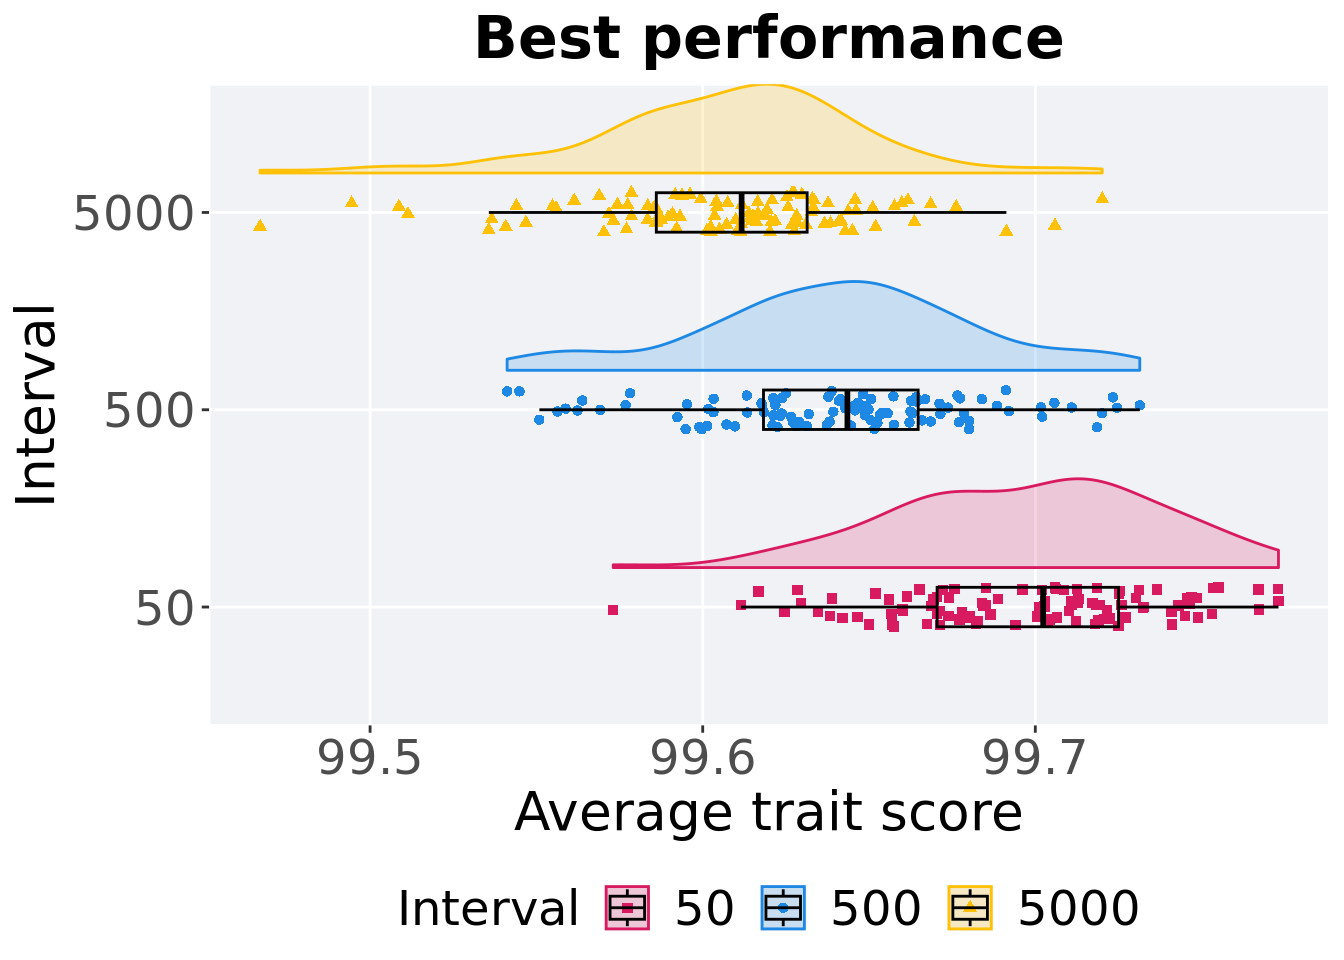
\includegraphics{demo_files/figure-latex/int-lex-ord-fit-1.pdf}

\hypertarget{stats-6}{%
\subsection{Stats}\label{stats-6}}

Summary statistics for the first generation a satisfactory solution is found.

\begin{Shaded}
\begin{Highlighting}[]
\NormalTok{best =}\StringTok{ }\KeywordTok{filter}\NormalTok{(df_best, Diagnostic }\OperatorTok{==}\StringTok{ 'ORDERED_EXPLOITATION'} \OperatorTok{&}\StringTok{ `}\DataTypeTok{Selection}\CharTok{\textbackslash{}n}\DataTypeTok{Scheme}\StringTok{`} \OperatorTok{==}\StringTok{ 'LEXICASE'} \OperatorTok{&}\StringTok{ }\NormalTok{VAR }\OperatorTok{==}\StringTok{ 'pop_fit_max'}\NormalTok{)}
\NormalTok{best }\OperatorTok
\StringTok{  }\KeywordTok{group_by}\NormalTok{(Interval) }\OperatorTok
\StringTok{  }\NormalTok{dplyr}\OperatorTok{::}\KeywordTok{summarise}\NormalTok{(}
    \DataTypeTok{count =} \KeywordTok{n}\NormalTok{(),}
    \DataTypeTok{na_cnt =} \KeywordTok{sum}\NormalTok{(}\KeywordTok{is.na}\NormalTok{(VAL)) }\OperatorTok{/}\StringTok{ }\NormalTok{DIMENSIONALITY,}
    \DataTypeTok{min =} \KeywordTok{min}\NormalTok{(VAL, }\DataTypeTok{na.rm =} \OtherTok{TRUE}\NormalTok{) }\OperatorTok{/}\StringTok{ }\NormalTok{DIMENSIONALITY,}
    \DataTypeTok{median =} \KeywordTok{median}\NormalTok{(VAL, }\DataTypeTok{na.rm =} \OtherTok{TRUE}\NormalTok{) }\OperatorTok{/}\StringTok{ }\NormalTok{DIMENSIONALITY,}
    \DataTypeTok{mean =} \KeywordTok{mean}\NormalTok{(VAL, }\DataTypeTok{na.rm =} \OtherTok{TRUE}\NormalTok{) }\OperatorTok{/}\StringTok{ }\NormalTok{DIMENSIONALITY,}
    \DataTypeTok{max =} \KeywordTok{max}\NormalTok{(VAL, }\DataTypeTok{na.rm =} \OtherTok{TRUE}\NormalTok{) }\OperatorTok{/}\StringTok{ }\NormalTok{DIMENSIONALITY,}
    \DataTypeTok{IQR =} \KeywordTok{IQR}\NormalTok{(VAL, }\DataTypeTok{na.rm =} \OtherTok{TRUE}\NormalTok{) }\OperatorTok{/}\StringTok{ }\NormalTok{DIMENSIONALITY}
\NormalTok{  )}
\end{Highlighting}
\end{Shaded}

\begin{verbatim}
## # A tibble: 3 x 8
##   Interval count na_cnt   min median  mean   max    IQR
##   <fct>    <int>  <dbl> <dbl>  <dbl> <dbl> <dbl>  <dbl>
## 1 50         100      0  99.6   99.7  99.7  99.8 0.0545
## 2 500        100      0  99.5   99.6  99.6  99.7 0.0465
## 3 5000       100      0  99.5   99.6  99.6  99.7 0.0454
\end{verbatim}

Kruskal--Wallis test provides evidence of difference among selection schemes.

\begin{Shaded}
\begin{Highlighting}[]
\KeywordTok{kruskal.test}\NormalTok{(VAL }\OperatorTok{~}\StringTok{ }\NormalTok{Interval, }\DataTypeTok{data =}\NormalTok{ best)}
\end{Highlighting}
\end{Shaded}

\begin{verbatim}
## 
##  Kruskal-Wallis rank sum test
## 
## data:  VAL by Interval
## Kruskal-Wallis chi-squared = 143.15, df = 2, p-value < 2.2e-16
\end{verbatim}

Results for post-hoc Wilcoxon rank-sum test with a Bonferroni correction.

\begin{Shaded}
\begin{Highlighting}[]
\KeywordTok{pairwise.wilcox.test}\NormalTok{(}\DataTypeTok{x =}\NormalTok{ best}\OperatorTok{$}\NormalTok{VAL, }\DataTypeTok{g =}\NormalTok{ best}\OperatorTok{$}\NormalTok{Interval, }\DataTypeTok{p.adjust.method =} \StringTok{"bonferroni"}\NormalTok{,}
                     \DataTypeTok{paired =} \OtherTok{FALSE}\NormalTok{, }\DataTypeTok{conf.int =} \OtherTok{FALSE}\NormalTok{, }\DataTypeTok{alternative =} \StringTok{'l'}\NormalTok{)}
\end{Highlighting}
\end{Shaded}

\begin{verbatim}
## 
##  Pairwise comparisons using Wilcoxon rank sum test with continuity correction 
## 
## data:  best$VAL and best$Interval 
## 
##      50      500    
## 500  < 2e-16 -      
## 5000 < 2e-16 6.4e-08
## 
## P value adjustment method: bonferroni
\end{verbatim}

\hypertarget{mi500-contradictory-objectives-results}{%
\chapter{MI500: Contradictory objectives results}\label{mi500-contradictory-objectives-results}}

Here we present the results for the \textbf{satisfactory trait corverage} and \textbf{activation gene coverage} generated by each selection scheme replicate on the contradictory objectives diagnostic with our base configurations.
Note both of these values are gathered at the population-level.
Activation gene coverage refers to the count of unique activation genes in a given population; this gives us a range of integers between 0 and 100.
Satisfactory trait coverage refers to the count of unique satisfied traits in a given population; this gives us a range of integers between 0 and 100.
For our base configuration, there are 4 islands in a ring topology.
When migrations occur, two individuals are swapped (same position on each island) and guarantee that no solution can return to its original island.

\hypertarget{analysis-dependencies-2}{%
\section{Analysis dependencies}\label{analysis-dependencies-2}}

\begin{Shaded}
\begin{Highlighting}[]
\KeywordTok{library}\NormalTok{(ggplot2)}
\KeywordTok{library}\NormalTok{(cowplot)}
\KeywordTok{library}\NormalTok{(dplyr)}
\KeywordTok{library}\NormalTok{(PupillometryR)}
\end{Highlighting}
\end{Shaded}

\hypertarget{data-2}{%
\section{Data}\label{data-2}}

\begin{Shaded}
\begin{Highlighting}[]
\NormalTok{base   =}\StringTok{ }\KeywordTok{filter}\NormalTok{(base_over_time,   Diagnostic }\OperatorTok{==}\StringTok{ 'CONTRADICTORY_OBJECTIVES'} \OperatorTok{&}\StringTok{ }\NormalTok{Structure }\OperatorTok{==}\StringTok{ 'IS'}\NormalTok{)}
\NormalTok{mi50   =}\StringTok{ }\KeywordTok{filter}\NormalTok{(mi50_over_time,   Diagnostic }\OperatorTok{==}\StringTok{ 'CONTRADICTORY_OBJECTIVES'} \OperatorTok{&}\StringTok{ }\NormalTok{Structure }\OperatorTok{==}\StringTok{ 'IS'}\NormalTok{)}
\NormalTok{mi5000 =}\StringTok{ }\KeywordTok{filter}\NormalTok{(mi5000_over_time, Diagnostic }\OperatorTok{==}\StringTok{ 'CONTRADICTORY_OBJECTIVES'} \OperatorTok{&}\StringTok{ }\NormalTok{Structure }\OperatorTok{==}\StringTok{ 'IS'}\NormalTok{)}

\NormalTok{base}\OperatorTok{$}\NormalTok{Interval =}\StringTok{ '500'}
\NormalTok{mi50}\OperatorTok{$}\NormalTok{Interval =}\StringTok{ '50'}
\NormalTok{mi5000}\OperatorTok{$}\NormalTok{Interval =}\StringTok{ '5000'}

\NormalTok{df_ot =}\StringTok{ }\KeywordTok{rbind}\NormalTok{(base, mi50, mi5000)}
\NormalTok{df_ot}\OperatorTok{$}\NormalTok{Interval =}\StringTok{ }\KeywordTok{factor}\NormalTok{(df_ot}\OperatorTok{$}\NormalTok{Interval, }\DataTypeTok{levels=}\KeywordTok{c}\NormalTok{(}\StringTok{'50'}\NormalTok{,}\StringTok{'500'}\NormalTok{,}\StringTok{'5000'}\NormalTok{))}

\NormalTok{base =}\StringTok{ }\KeywordTok{filter}\NormalTok{(base_best,     Diagnostic }\OperatorTok{==}\StringTok{ 'CONTRADICTORY_OBJECTIVES'} \OperatorTok{&}\StringTok{ }\NormalTok{Structure }\OperatorTok{==}\StringTok{ 'IS'}\NormalTok{)}
\NormalTok{mi50 =}\StringTok{ }\KeywordTok{filter}\NormalTok{(mi50_best,     Diagnostic }\OperatorTok{==}\StringTok{ 'CONTRADICTORY_OBJECTIVES'} \OperatorTok{&}\StringTok{ }\NormalTok{Structure }\OperatorTok{==}\StringTok{ 'IS'}\NormalTok{)}
\NormalTok{mi5000 =}\StringTok{ }\KeywordTok{filter}\NormalTok{(mi5000_best, Diagnostic }\OperatorTok{==}\StringTok{ 'CONTRADICTORY_OBJECTIVES'} \OperatorTok{&}\StringTok{ }\NormalTok{Structure }\OperatorTok{==}\StringTok{ 'IS'}\NormalTok{)}

\NormalTok{base}\OperatorTok{$}\NormalTok{Interval =}\StringTok{ '500'}
\NormalTok{mi50}\OperatorTok{$}\NormalTok{Interval =}\StringTok{ '50'}
\NormalTok{mi5000}\OperatorTok{$}\NormalTok{Interval =}\StringTok{ '5000'}

\NormalTok{df_best =}\StringTok{ }\KeywordTok{rbind}\NormalTok{(mi50,base,mi5000)}
\NormalTok{df_best}\OperatorTok{$}\NormalTok{Interval =}\StringTok{ }\KeywordTok{factor}\NormalTok{(df_best}\OperatorTok{$}\NormalTok{Interval, }\DataTypeTok{levels =} \KeywordTok{c}\NormalTok{(}\StringTok{'50'}\NormalTok{,}\StringTok{'500'}\NormalTok{,}\StringTok{'5000'}\NormalTok{))}
\end{Highlighting}
\end{Shaded}

\hypertarget{truncation-selection-2}{%
\section{Truncation selection}\label{truncation-selection-2}}

Here we analyze how the different population structures affect truncation selection (size 8) on the contradictory objectives diagnostic.

\hypertarget{satisfactory-trait-coverage}{%
\subsection{Satisfactory trait coverage}\label{satisfactory-trait-coverage}}

Satisfactory trait coverage analysis.

\hypertarget{coverage-over-time}{%
\subsubsection{Coverage over time}\label{coverage-over-time}}

Satisfactory trait coverage over time.

\begin{Shaded}
\begin{Highlighting}[]
\NormalTok{lines =}\StringTok{ }\KeywordTok{filter}\NormalTok{(df_ot,}\StringTok{`}\DataTypeTok{Selection}\CharTok{\textbackslash{}n}\DataTypeTok{Scheme}\StringTok{`} \OperatorTok{==}\StringTok{ 'TRUNCATION'}\NormalTok{) }\OperatorTok
\StringTok{  }\KeywordTok{group_by}\NormalTok{(Interval, Generations) }\OperatorTok
\StringTok{  }\NormalTok{dplyr}\OperatorTok{::}\KeywordTok{summarise}\NormalTok{(}
    \DataTypeTok{min =} \KeywordTok{min}\NormalTok{(pop_sat_cov),}
    \DataTypeTok{mean =} \KeywordTok{mean}\NormalTok{(pop_sat_cov),}
    \DataTypeTok{max =} \KeywordTok{max}\NormalTok{(pop_sat_cov)}
\NormalTok{  )}
\end{Highlighting}
\end{Shaded}

\begin{verbatim}
## `summarise()` has grouped output by 'Interval'. You can override using the
## `.groups` argument.
\end{verbatim}

\begin{Shaded}
\begin{Highlighting}[]
\KeywordTok{ggplot}\NormalTok{(lines, }\KeywordTok{aes}\NormalTok{(}\DataTypeTok{x=}\NormalTok{Generations, }\DataTypeTok{y=}\NormalTok{mean, }\DataTypeTok{group =}\NormalTok{ Interval, }\DataTypeTok{fill =}\NormalTok{ Interval, }\DataTypeTok{color =}\NormalTok{ Interval, }\DataTypeTok{shape =}\NormalTok{ Interval)) }\OperatorTok{+}
\StringTok{  }\KeywordTok{geom_ribbon}\NormalTok{(}\KeywordTok{aes}\NormalTok{(}\DataTypeTok{ymin =}\NormalTok{ min, }\DataTypeTok{ymax =}\NormalTok{ max), }\DataTypeTok{alpha =} \FloatTok{0.1}\NormalTok{) }\OperatorTok{+}
\StringTok{  }\KeywordTok{geom_line}\NormalTok{(}\DataTypeTok{size =} \FloatTok{0.5}\NormalTok{) }\OperatorTok{+}
\StringTok{  }\KeywordTok{geom_point}\NormalTok{(}\DataTypeTok{data =} \KeywordTok{filter}\NormalTok{(lines, Generations }\OperatorTok\StringTok{ }\DecValTok{2000} \OperatorTok{==}\StringTok{ }\DecValTok{0}\NormalTok{), }\DataTypeTok{size =} \FloatTok{1.5}\NormalTok{, }\DataTypeTok{stroke =} \FloatTok{2.0}\NormalTok{, }\DataTypeTok{alpha =} \FloatTok{1.0}\NormalTok{) }\OperatorTok{+}
\StringTok{  }\KeywordTok{scale_y_continuous}\NormalTok{(}
    \DataTypeTok{name=}\StringTok{"Coverage"}
\NormalTok{  ) }\OperatorTok{+}
\StringTok{  }\KeywordTok{scale_x_continuous}\NormalTok{(}
    \DataTypeTok{name=}\StringTok{"Generations"}\NormalTok{,}
    \DataTypeTok{limits=}\KeywordTok{c}\NormalTok{(}\DecValTok{0}\NormalTok{, }\DecValTok{50000}\NormalTok{),}
    \DataTypeTok{breaks=}\KeywordTok{c}\NormalTok{(}\DecValTok{0}\NormalTok{, }\DecValTok{10000}\NormalTok{, }\DecValTok{20000}\NormalTok{, }\DecValTok{30000}\NormalTok{, }\DecValTok{40000}\NormalTok{, }\DecValTok{50000}\NormalTok{),}
    \DataTypeTok{labels=}\KeywordTok{c}\NormalTok{(}\StringTok{"0e+4"}\NormalTok{, }\StringTok{"1e+4"}\NormalTok{, }\StringTok{"2e+4"}\NormalTok{, }\StringTok{"3e+4"}\NormalTok{, }\StringTok{"4e+4"}\NormalTok{, }\StringTok{"5e+4"}\NormalTok{)}

\NormalTok{  ) }\OperatorTok{+}
\StringTok{  }\KeywordTok{scale_shape_manual}\NormalTok{(}\DataTypeTok{values=}\NormalTok{SHAPE)}\OperatorTok{+}
\StringTok{  }\KeywordTok{scale_colour_manual}\NormalTok{(}\DataTypeTok{values =}\NormalTok{ cb_palette_mi) }\OperatorTok{+}
\StringTok{  }\KeywordTok{scale_fill_manual}\NormalTok{(}\DataTypeTok{values =}\NormalTok{ cb_palette_mi) }\OperatorTok{+}
\StringTok{  }\KeywordTok{ggtitle}\NormalTok{(}\StringTok{'Satisfactory trait coverage over time'}\NormalTok{)}\OperatorTok{+}
\StringTok{  }\NormalTok{p_theme}
\end{Highlighting}
\end{Shaded}

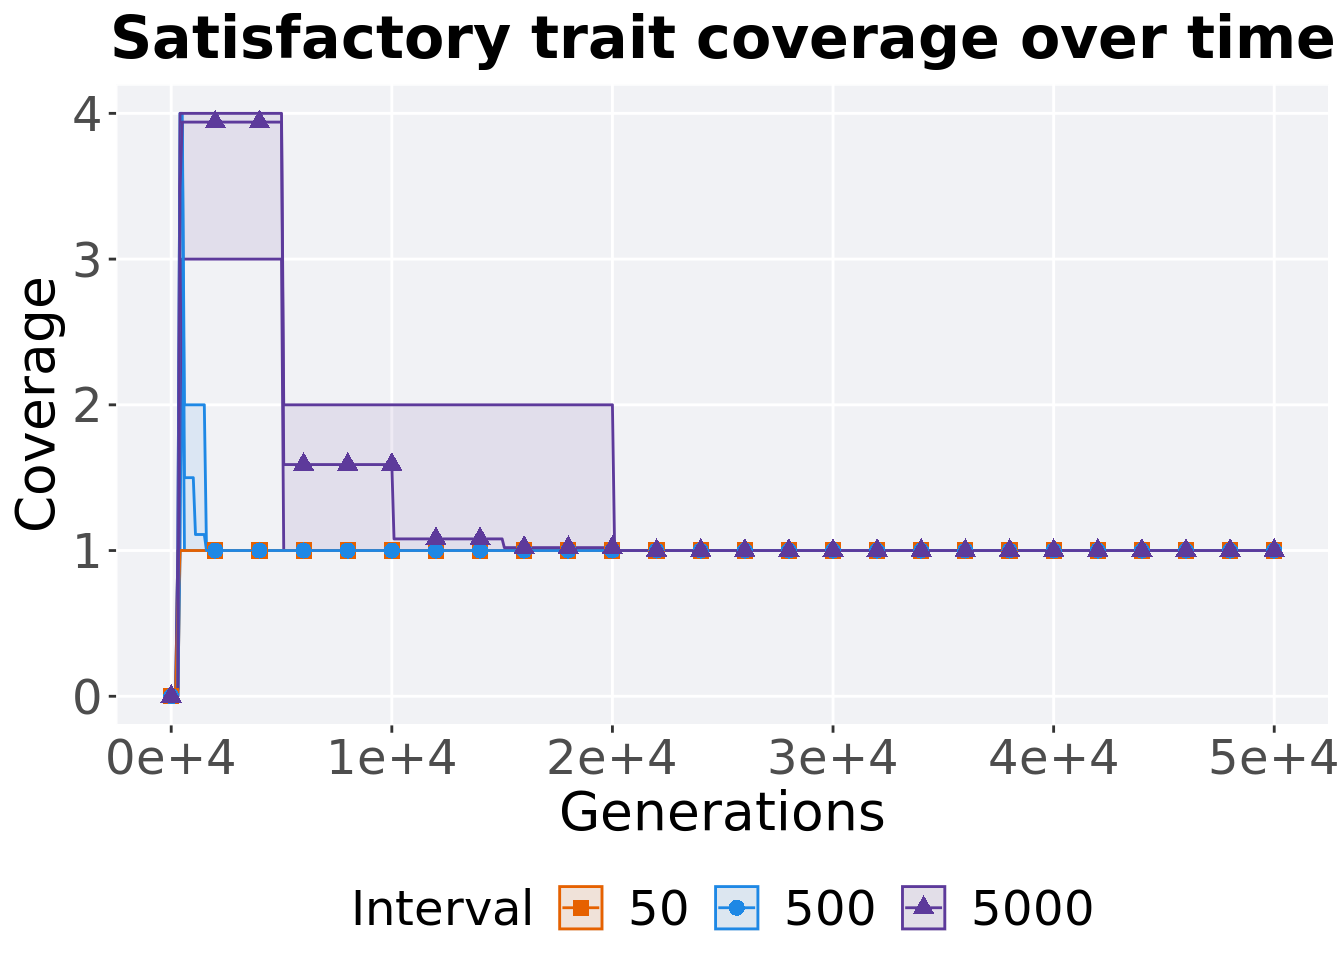
\includegraphics{demo_files/figure-latex/int-con-sat-tru-ot-1.pdf}

\hypertarget{best-coverage-throughout}{%
\subsubsection{Best coverage throughout}\label{best-coverage-throughout}}

Best satisfactory trait coverage throughout 50,000 generations.

\begin{Shaded}
\begin{Highlighting}[]
\CommentTok{### best satisfactory trait coverage throughout}
\KeywordTok{filter}\NormalTok{(df_best, Diagnostic }\OperatorTok{==}\StringTok{ 'CONTRADICTORY_OBJECTIVES'} \OperatorTok{&}\StringTok{ `}\DataTypeTok{Selection}\CharTok{\textbackslash{}n}\DataTypeTok{Scheme}\StringTok{`} \OperatorTok{==}\StringTok{ 'TRUNCATION'} \OperatorTok{&}\StringTok{ }\NormalTok{VAR }\OperatorTok{==}\StringTok{ 'pop_sat_cov'}\NormalTok{) }\OperatorTok
\StringTok{  }\KeywordTok{ggplot}\NormalTok{(., }\KeywordTok{aes}\NormalTok{(}\DataTypeTok{x =}\NormalTok{ Interval, }\DataTypeTok{y =}\NormalTok{ VAL, }\DataTypeTok{color =}\NormalTok{ Interval, }\DataTypeTok{fill =}\NormalTok{ Interval, }\DataTypeTok{shape =}\NormalTok{ Interval)) }\OperatorTok{+}
\StringTok{  }\KeywordTok{geom_flat_violin}\NormalTok{(}\DataTypeTok{position =} \KeywordTok{position_nudge}\NormalTok{(}\DataTypeTok{x =} \FloatTok{.2}\NormalTok{, }\DataTypeTok{y =} \DecValTok{0}\NormalTok{), }\DataTypeTok{scale =} \StringTok{'width'}\NormalTok{, }\DataTypeTok{alpha =} \FloatTok{0.2}\NormalTok{) }\OperatorTok{+}
\StringTok{  }\KeywordTok{geom_point}\NormalTok{(}\DataTypeTok{position =} \KeywordTok{position_jitter}\NormalTok{(}\DataTypeTok{height =} \FloatTok{.05}\NormalTok{, }\DataTypeTok{width =} \FloatTok{.05}\NormalTok{), }\DataTypeTok{size =} \FloatTok{1.5}\NormalTok{, }\DataTypeTok{alpha =} \FloatTok{1.0}\NormalTok{) }\OperatorTok{+}
\StringTok{  }\KeywordTok{geom_boxplot}\NormalTok{(}\DataTypeTok{color =} \StringTok{'black'}\NormalTok{, }\DataTypeTok{width =} \FloatTok{.2}\NormalTok{, }\DataTypeTok{outlier.shape =} \OtherTok{NA}\NormalTok{, }\DataTypeTok{alpha =} \FloatTok{0.0}\NormalTok{) }\OperatorTok{+}
\StringTok{  }\KeywordTok{scale_y_continuous}\NormalTok{(}
    \DataTypeTok{name=}\StringTok{"coverage"}
\NormalTok{  ) }\OperatorTok{+}
\StringTok{  }\KeywordTok{scale_x_discrete}\NormalTok{(}
    \DataTypeTok{name=}\StringTok{"Interval"}
\NormalTok{  )}\OperatorTok{+}
\StringTok{  }\KeywordTok{scale_shape_manual}\NormalTok{(}\DataTypeTok{values=}\NormalTok{SHAPE)}\OperatorTok{+}
\StringTok{  }\KeywordTok{scale_colour_manual}\NormalTok{(}\DataTypeTok{values =}\NormalTok{ cb_palette_mi, ) }\OperatorTok{+}
\StringTok{  }\KeywordTok{scale_fill_manual}\NormalTok{(}\DataTypeTok{values =}\NormalTok{ cb_palette_mi) }\OperatorTok{+}
\StringTok{  }\KeywordTok{ggtitle}\NormalTok{(}\StringTok{'Best satisfactory trait coverage'}\NormalTok{)}\OperatorTok{+}
\StringTok{  }\NormalTok{p_theme }\OperatorTok{+}\StringTok{ }\KeywordTok{coord_flip}\NormalTok{()}
\end{Highlighting}
\end{Shaded}

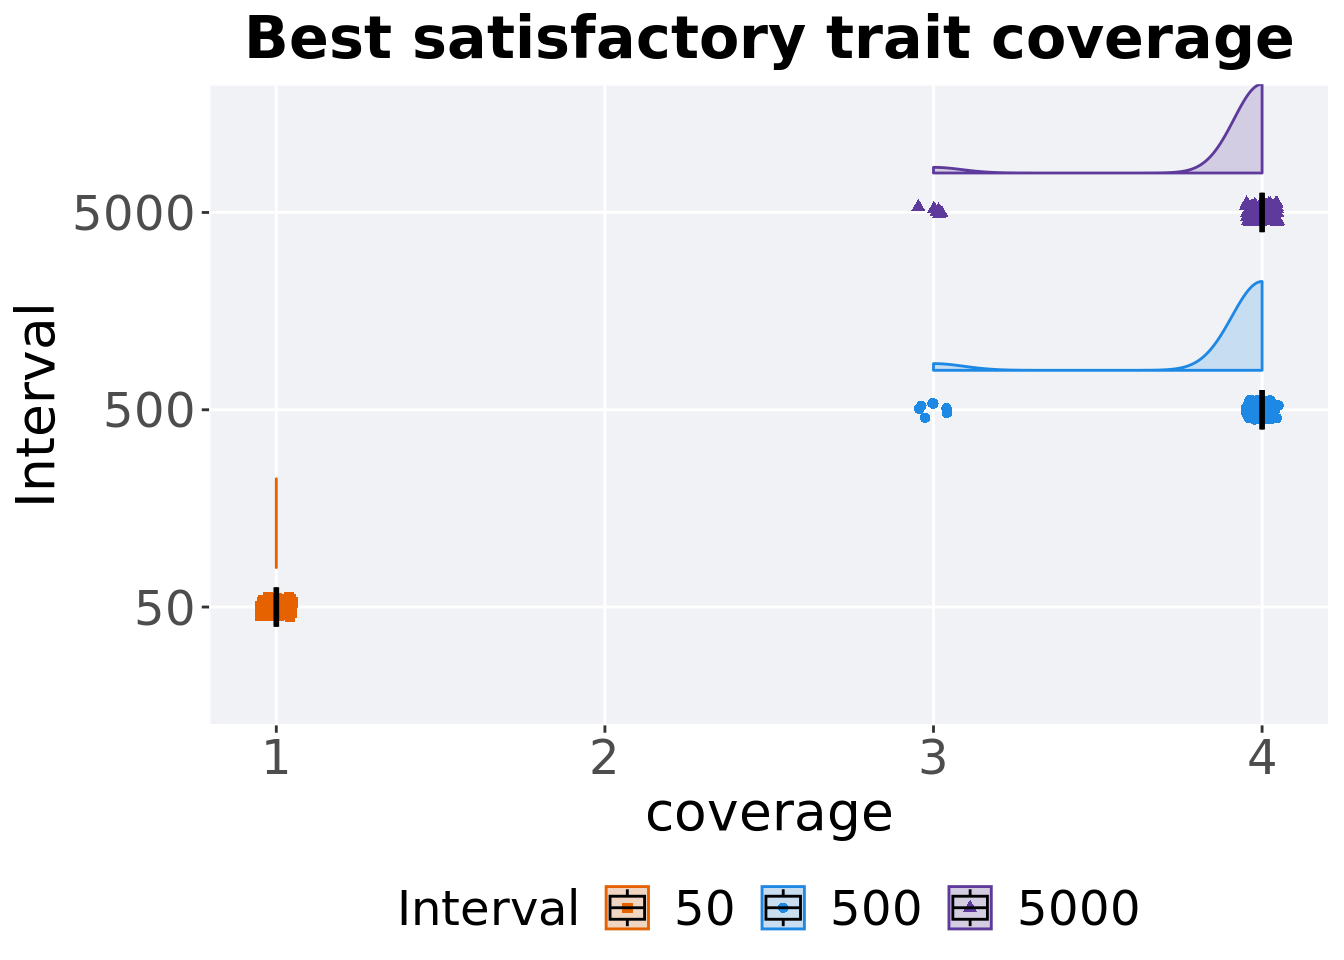
\includegraphics{demo_files/figure-latex/int-con-sat-tru-bst-1.pdf}

\hypertarget{stats-7}{%
\paragraph{Stats}\label{stats-7}}

Summary statistics for the best satisfactory trait coverage.

\begin{Shaded}
\begin{Highlighting}[]
\CommentTok{### best}
\NormalTok{coverage =}\StringTok{ }\KeywordTok{filter}\NormalTok{(df_best, Diagnostic }\OperatorTok{==}\StringTok{ 'CONTRADICTORY_OBJECTIVES'} \OperatorTok{&}\StringTok{ `}\DataTypeTok{Selection}\CharTok{\textbackslash{}n}\DataTypeTok{Scheme}\StringTok{`} \OperatorTok{==}\StringTok{ 'TRUNCATION'} \OperatorTok{&}\StringTok{ }\NormalTok{VAR }\OperatorTok{==}\StringTok{ 'pop_sat_cov'}\NormalTok{)}
\NormalTok{coverage }\OperatorTok
\StringTok{  }\KeywordTok{group_by}\NormalTok{(Interval) }\OperatorTok
\StringTok{  }\NormalTok{dplyr}\OperatorTok{::}\KeywordTok{summarise}\NormalTok{(}
    \DataTypeTok{count =} \KeywordTok{n}\NormalTok{(),}
    \DataTypeTok{na_cnt =} \KeywordTok{sum}\NormalTok{(}\KeywordTok{is.na}\NormalTok{(VAL)),}
    \DataTypeTok{min =} \KeywordTok{min}\NormalTok{(VAL, }\DataTypeTok{na.rm =} \OtherTok{TRUE}\NormalTok{),}
    \DataTypeTok{median =} \KeywordTok{median}\NormalTok{(VAL, }\DataTypeTok{na.rm =} \OtherTok{TRUE}\NormalTok{),}
    \DataTypeTok{mean =} \KeywordTok{mean}\NormalTok{(VAL, }\DataTypeTok{na.rm =} \OtherTok{TRUE}\NormalTok{),}
    \DataTypeTok{max =} \KeywordTok{max}\NormalTok{(VAL, }\DataTypeTok{na.rm =} \OtherTok{TRUE}\NormalTok{),}
    \DataTypeTok{IQR =} \KeywordTok{IQR}\NormalTok{(VAL, }\DataTypeTok{na.rm =} \OtherTok{TRUE}\NormalTok{)}
\NormalTok{  )}
\end{Highlighting}
\end{Shaded}

\begin{verbatim}
## # A tibble: 3 x 8
##   Interval count na_cnt   min median  mean   max   IQR
##   <fct>    <int>  <int> <dbl>  <dbl> <dbl> <dbl> <dbl>
## 1 50         100      0     1      1  1        1     0
## 2 500        100      0     3      4  3.93     4     0
## 3 5000       100      0     3      4  3.94     4     0
\end{verbatim}

Kruskal--Wallis test provides evidence of difference among satisfactory trait coverage.

\begin{Shaded}
\begin{Highlighting}[]
\KeywordTok{kruskal.test}\NormalTok{(VAL }\OperatorTok{~}\StringTok{ }\NormalTok{Interval, }\DataTypeTok{data =}\NormalTok{ coverage)}
\end{Highlighting}
\end{Shaded}

\begin{verbatim}
## 
##  Kruskal-Wallis rank sum test
## 
## data:  VAL by Interval
## Kruskal-Wallis chi-squared = 276.6, df = 2, p-value < 2.2e-16
\end{verbatim}

Results for post-hoc Wilcoxon rank-sum test with a Bonferroni correction on satisfactory trait coverage.

\begin{Shaded}
\begin{Highlighting}[]
\KeywordTok{pairwise.wilcox.test}\NormalTok{(}\DataTypeTok{x =}\NormalTok{ coverage}\OperatorTok{$}\NormalTok{VAL, }\DataTypeTok{g =}\NormalTok{ coverage}\OperatorTok{$}\NormalTok{Interval, }\DataTypeTok{p.adjust.method =} \StringTok{"bonferroni"}\NormalTok{,}
                     \DataTypeTok{paired =} \OtherTok{FALSE}\NormalTok{, }\DataTypeTok{conf.int =} \OtherTok{FALSE}\NormalTok{, }\DataTypeTok{alternative =} \StringTok{'g'}\NormalTok{)}
\end{Highlighting}
\end{Shaded}

\begin{verbatim}
## 
##  Pairwise comparisons using Wilcoxon rank sum test with continuity correction 
## 
## data:  coverage$VAL and coverage$Interval 
## 
##      50     500
## 500  <2e-16 -  
## 5000 <2e-16 1  
## 
## P value adjustment method: bonferroni
\end{verbatim}

\hypertarget{end-of-50000-generations}{%
\subsubsection{End of 50,000 generations}\label{end-of-50000-generations}}

Satisfactory trait coverage in the population at the end of 50,000 generations.

\begin{Shaded}
\begin{Highlighting}[]
\CommentTok{### end of run}
\KeywordTok{filter}\NormalTok{(df_ot, Diagnostic }\OperatorTok{==}\StringTok{ 'CONTRADICTORY_OBJECTIVES'} \OperatorTok{&}\StringTok{ `}\DataTypeTok{Selection}\CharTok{\textbackslash{}n}\DataTypeTok{Scheme}\StringTok{`} \OperatorTok{==}\StringTok{ 'TRUNCATION'} \OperatorTok{&}\StringTok{ }\NormalTok{Generations }\OperatorTok{==}\StringTok{ }\DecValTok{50000}\NormalTok{) }\OperatorTok
\StringTok{  }\KeywordTok{ggplot}\NormalTok{(., }\KeywordTok{aes}\NormalTok{(}\DataTypeTok{x =}\NormalTok{ Interval, }\DataTypeTok{y =}\NormalTok{ pop_sat_cov, }\DataTypeTok{color =}\NormalTok{ Interval, }\DataTypeTok{fill =}\NormalTok{ Interval, }\DataTypeTok{shape =}\NormalTok{ Interval)) }\OperatorTok{+}
\StringTok{  }\KeywordTok{geom_flat_violin}\NormalTok{(}\DataTypeTok{position =} \KeywordTok{position_nudge}\NormalTok{(}\DataTypeTok{x =} \FloatTok{.2}\NormalTok{, }\DataTypeTok{y =} \DecValTok{0}\NormalTok{), }\DataTypeTok{scale =} \StringTok{'width'}\NormalTok{, }\DataTypeTok{alpha =} \FloatTok{0.3}\NormalTok{) }\OperatorTok{+}
\StringTok{  }\KeywordTok{geom_point}\NormalTok{(}\DataTypeTok{position =} \KeywordTok{position_jitter}\NormalTok{(}\DataTypeTok{height =} \FloatTok{.05}\NormalTok{, }\DataTypeTok{width =} \FloatTok{.05}\NormalTok{), }\DataTypeTok{size =} \FloatTok{1.5}\NormalTok{, }\DataTypeTok{alpha =} \FloatTok{0.5}\NormalTok{) }\OperatorTok{+}
\StringTok{  }\KeywordTok{geom_boxplot}\NormalTok{(}\DataTypeTok{color =} \StringTok{'black'}\NormalTok{, }\DataTypeTok{width =} \FloatTok{.2}\NormalTok{, }\DataTypeTok{outlier.shape =} \OtherTok{NA}\NormalTok{, }\DataTypeTok{alpha =} \FloatTok{0.0}\NormalTok{) }\OperatorTok{+}
\StringTok{  }\KeywordTok{scale_shape_manual}\NormalTok{(}\DataTypeTok{values=}\NormalTok{SHAPE)}\OperatorTok{+}
\StringTok{  }\KeywordTok{scale_y_continuous}\NormalTok{(}
    \DataTypeTok{name=}\StringTok{"Coverage"}
\NormalTok{  ) }\OperatorTok{+}
\StringTok{  }\KeywordTok{scale_x_discrete}\NormalTok{(}
    \DataTypeTok{name=}\StringTok{"Interval"}
\NormalTok{  ) }\OperatorTok{+}
\StringTok{  }\KeywordTok{scale_colour_manual}\NormalTok{(}\DataTypeTok{values =}\NormalTok{ cb_palette_mi) }\OperatorTok{+}
\StringTok{  }\KeywordTok{scale_fill_manual}\NormalTok{(}\DataTypeTok{values =}\NormalTok{ cb_palette_mi) }\OperatorTok{+}
\StringTok{  }\KeywordTok{ggtitle}\NormalTok{(}\StringTok{'Final satisfactory trait coverage'}\NormalTok{)}\OperatorTok{+}
\StringTok{  }\NormalTok{p_theme }\OperatorTok{+}\StringTok{ }\KeywordTok{coord_flip}\NormalTok{()}
\end{Highlighting}
\end{Shaded}

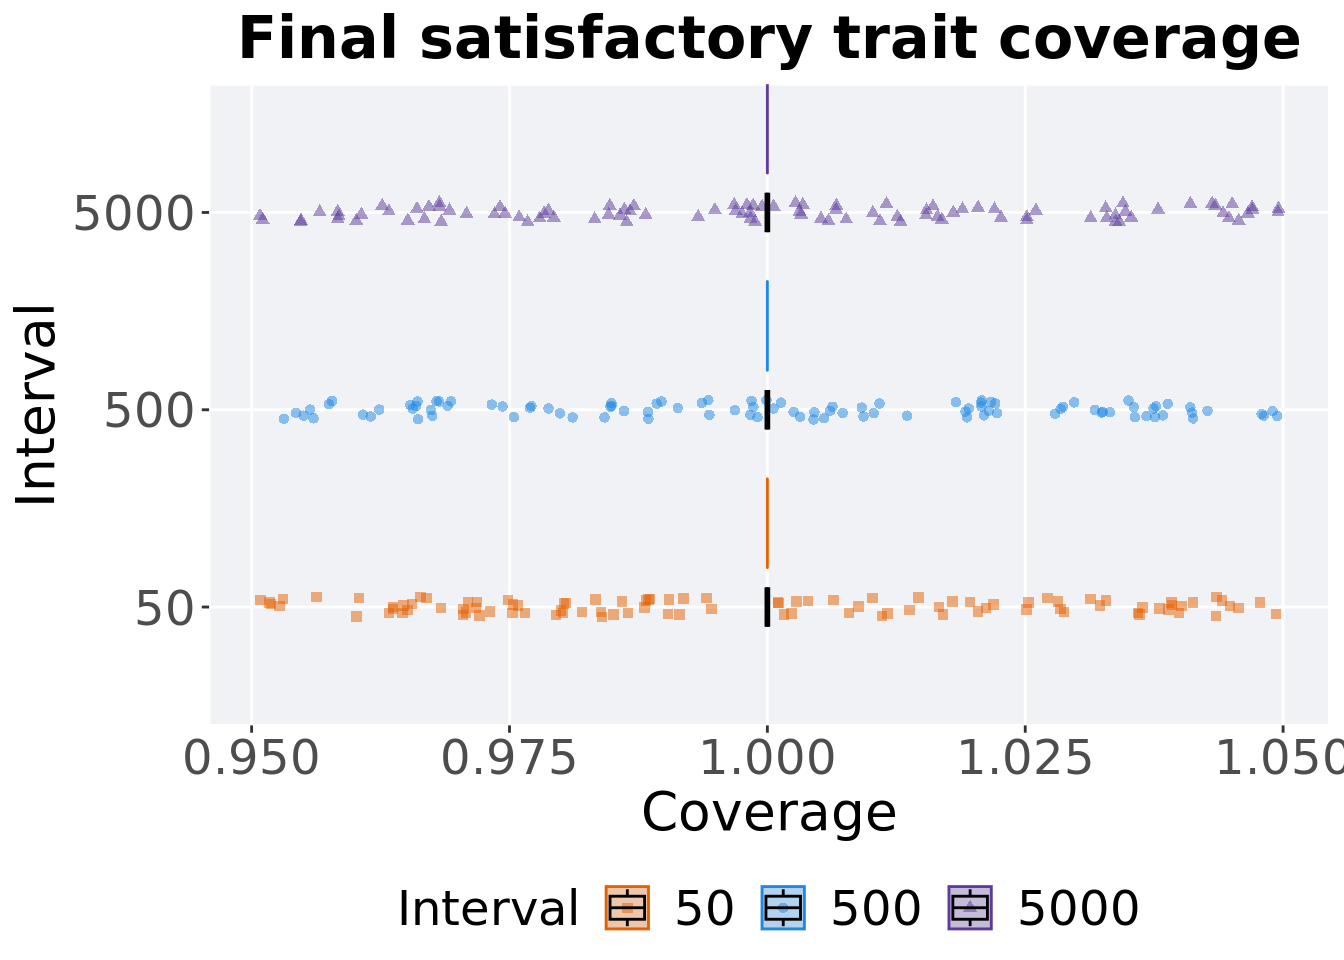
\includegraphics{demo_files/figure-latex/int-con-sat-tru-end-1.pdf}

\hypertarget{stats-8}{%
\paragraph{Stats}\label{stats-8}}

Summary statistics for satisfactory trait coverage in the population at the end of 50,000 generations.

\begin{Shaded}
\begin{Highlighting}[]
\CommentTok{### end of run}
\NormalTok{coverage =}\StringTok{ }\KeywordTok{filter}\NormalTok{(df_ot, Diagnostic }\OperatorTok{==}\StringTok{ 'CONTRADICTORY_OBJECTIVES'} \OperatorTok{&}\StringTok{ `}\DataTypeTok{Selection}\CharTok{\textbackslash{}n}\DataTypeTok{Scheme}\StringTok{`} \OperatorTok{==}\StringTok{ 'TRUNCATION'} \OperatorTok{&}\StringTok{ }\NormalTok{Generations }\OperatorTok{==}\StringTok{ }\DecValTok{50000}\NormalTok{)}
\NormalTok{coverage }\OperatorTok
\StringTok{  }\KeywordTok{group_by}\NormalTok{(Interval) }\OperatorTok
\StringTok{  }\NormalTok{dplyr}\OperatorTok{::}\KeywordTok{summarise}\NormalTok{(}
    \DataTypeTok{count =} \KeywordTok{n}\NormalTok{(),}
    \DataTypeTok{na_cnt =} \KeywordTok{sum}\NormalTok{(}\KeywordTok{is.na}\NormalTok{(pop_sat_cov)),}
    \DataTypeTok{min =} \KeywordTok{min}\NormalTok{(pop_sat_cov, }\DataTypeTok{na.rm =} \OtherTok{TRUE}\NormalTok{),}
    \DataTypeTok{median =} \KeywordTok{median}\NormalTok{(pop_sat_cov, }\DataTypeTok{na.rm =} \OtherTok{TRUE}\NormalTok{),}
    \DataTypeTok{mean =} \KeywordTok{mean}\NormalTok{(pop_sat_cov, }\DataTypeTok{na.rm =} \OtherTok{TRUE}\NormalTok{),}
    \DataTypeTok{max =} \KeywordTok{max}\NormalTok{(pop_sat_cov, }\DataTypeTok{na.rm =} \OtherTok{TRUE}\NormalTok{),}
    \DataTypeTok{IQR =} \KeywordTok{IQR}\NormalTok{(pop_sat_cov, }\DataTypeTok{na.rm =} \OtherTok{TRUE}\NormalTok{)}
\NormalTok{  )}
\end{Highlighting}
\end{Shaded}

\begin{verbatim}
## # A tibble: 3 x 8
##   Interval count na_cnt   min median  mean   max   IQR
##   <fct>    <int>  <int> <int>  <dbl> <dbl> <int> <dbl>
## 1 50         100      0     1      1     1     1     0
## 2 500        100      0     1      1     1     1     0
## 3 5000       100      0     1      1     1     1     0
\end{verbatim}

Kruskal--Wallis test provides evidence of difference among satisfactory trait coverage in the population at the end of 50,000 generations.

\begin{Shaded}
\begin{Highlighting}[]
\KeywordTok{kruskal.test}\NormalTok{(pop_sat_cov }\OperatorTok{~}\StringTok{ }\NormalTok{Interval, }\DataTypeTok{data =}\NormalTok{ coverage)}
\end{Highlighting}
\end{Shaded}

\begin{verbatim}
## 
##  Kruskal-Wallis rank sum test
## 
## data:  pop_sat_cov by Interval
## Kruskal-Wallis chi-squared = NaN, df = 2, p-value = NA
\end{verbatim}

Results for post-hoc Wilcoxon rank-sum test with a Bonferroni correction on satisfactory trait coverage in the population at the end of 50,000 generations.

\begin{Shaded}
\begin{Highlighting}[]
\KeywordTok{pairwise.wilcox.test}\NormalTok{(}\DataTypeTok{x =}\NormalTok{ coverage}\OperatorTok{$}\NormalTok{pop_sat_cov, }\DataTypeTok{g =}\NormalTok{ coverage}\OperatorTok{$}\NormalTok{Interval, }\DataTypeTok{p.adjust.method =} \StringTok{"bonferroni"}\NormalTok{,}
                     \DataTypeTok{paired =} \OtherTok{FALSE}\NormalTok{, }\DataTypeTok{conf.int =} \OtherTok{FALSE}\NormalTok{, }\DataTypeTok{alternative =} \StringTok{'g'}\NormalTok{)}
\end{Highlighting}
\end{Shaded}

\begin{verbatim}
## 
##  Pairwise comparisons using Wilcoxon rank sum test with continuity correction 
## 
## data:  coverage$pop_sat_cov and coverage$Interval 
## 
##      50 500
## 500  1  -  
## 5000 1  1  
## 
## P value adjustment method: bonferroni
\end{verbatim}

\hypertarget{activation-gene-coverage}{%
\subsection{Activation gene coverage}\label{activation-gene-coverage}}

Activation gene coverage analysis.

\hypertarget{coverage-over-time-1}{%
\subsubsection{Coverage over time}\label{coverage-over-time-1}}

Activation gene coverage over time.

\begin{Shaded}
\begin{Highlighting}[]
\CommentTok{# data for lines and shading on plots}
\NormalTok{lines =}\StringTok{ }\KeywordTok{filter}\NormalTok{(df_ot, Diagnostic }\OperatorTok{==}\StringTok{ 'CONTRADICTORY_OBJECTIVES'} \OperatorTok{&}\StringTok{ `}\DataTypeTok{Selection}\CharTok{\textbackslash{}n}\DataTypeTok{Scheme}\StringTok{`} \OperatorTok{==}\StringTok{ 'TRUNCATION'}\NormalTok{) }\OperatorTok
\StringTok{  }\KeywordTok{group_by}\NormalTok{(Interval, Generations) }\OperatorTok
\StringTok{  }\NormalTok{dplyr}\OperatorTok{::}\KeywordTok{summarise}\NormalTok{(}
    \DataTypeTok{min =} \KeywordTok{min}\NormalTok{(pop_act_cov),}
    \DataTypeTok{mean =} \KeywordTok{mean}\NormalTok{(pop_act_cov),}
    \DataTypeTok{max =} \KeywordTok{max}\NormalTok{(pop_act_cov)}
\NormalTok{  )}
\end{Highlighting}
\end{Shaded}

\begin{verbatim}
## `summarise()` has grouped output by 'Interval'. You can override using the
## `.groups` argument.
\end{verbatim}

\begin{Shaded}
\begin{Highlighting}[]
\KeywordTok{ggplot}\NormalTok{(lines, }\KeywordTok{aes}\NormalTok{(}\DataTypeTok{x=}\NormalTok{Generations, }\DataTypeTok{y=}\NormalTok{mean, }\DataTypeTok{group =}\NormalTok{ Interval, }\DataTypeTok{fill =}\NormalTok{ Interval, }\DataTypeTok{color =}\NormalTok{ Interval, }\DataTypeTok{shape =}\NormalTok{ Interval)) }\OperatorTok{+}
\StringTok{  }\KeywordTok{geom_ribbon}\NormalTok{(}\KeywordTok{aes}\NormalTok{(}\DataTypeTok{ymin =}\NormalTok{ min, }\DataTypeTok{ymax =}\NormalTok{ max), }\DataTypeTok{alpha =} \FloatTok{0.1}\NormalTok{) }\OperatorTok{+}
\StringTok{  }\KeywordTok{geom_line}\NormalTok{(}\DataTypeTok{size =} \FloatTok{0.5}\NormalTok{) }\OperatorTok{+}
\StringTok{  }\KeywordTok{geom_point}\NormalTok{(}\DataTypeTok{data =} \KeywordTok{filter}\NormalTok{(lines, Generations }\OperatorTok\StringTok{ }\DecValTok{2000} \OperatorTok{==}\StringTok{ }\DecValTok{0}\NormalTok{), }\DataTypeTok{size =} \FloatTok{1.5}\NormalTok{, }\DataTypeTok{stroke =} \FloatTok{2.0}\NormalTok{, }\DataTypeTok{alpha =} \FloatTok{1.0}\NormalTok{) }\OperatorTok{+}
\StringTok{  }\KeywordTok{scale_y_continuous}\NormalTok{(}
    \DataTypeTok{name=}\StringTok{"Coverage"}
\NormalTok{  ) }\OperatorTok{+}
\StringTok{  }\KeywordTok{scale_x_continuous}\NormalTok{(}
    \DataTypeTok{name=}\StringTok{"Generations"}\NormalTok{,}
    \DataTypeTok{limits=}\KeywordTok{c}\NormalTok{(}\DecValTok{0}\NormalTok{, }\DecValTok{50000}\NormalTok{),}
    \DataTypeTok{breaks=}\KeywordTok{c}\NormalTok{(}\DecValTok{0}\NormalTok{, }\DecValTok{10000}\NormalTok{, }\DecValTok{20000}\NormalTok{, }\DecValTok{30000}\NormalTok{, }\DecValTok{40000}\NormalTok{, }\DecValTok{50000}\NormalTok{),}
    \DataTypeTok{labels=}\KeywordTok{c}\NormalTok{(}\StringTok{"0e+4"}\NormalTok{, }\StringTok{"1e+4"}\NormalTok{, }\StringTok{"2e+4"}\NormalTok{, }\StringTok{"3e+4"}\NormalTok{, }\StringTok{"4e+4"}\NormalTok{, }\StringTok{"5e+4"}\NormalTok{)}

\NormalTok{  ) }\OperatorTok{+}
\StringTok{  }\KeywordTok{scale_shape_manual}\NormalTok{(}\DataTypeTok{values=}\NormalTok{SHAPE)}\OperatorTok{+}
\StringTok{  }\KeywordTok{scale_colour_manual}\NormalTok{(}\DataTypeTok{values =}\NormalTok{ cb_palette_mi) }\OperatorTok{+}
\StringTok{  }\KeywordTok{scale_fill_manual}\NormalTok{(}\DataTypeTok{values =}\NormalTok{ cb_palette_mi) }\OperatorTok{+}
\StringTok{  }\KeywordTok{ggtitle}\NormalTok{(}\StringTok{'Activation gene coverage over time'}\NormalTok{)}\OperatorTok{+}
\StringTok{  }\NormalTok{p_theme}
\end{Highlighting}
\end{Shaded}

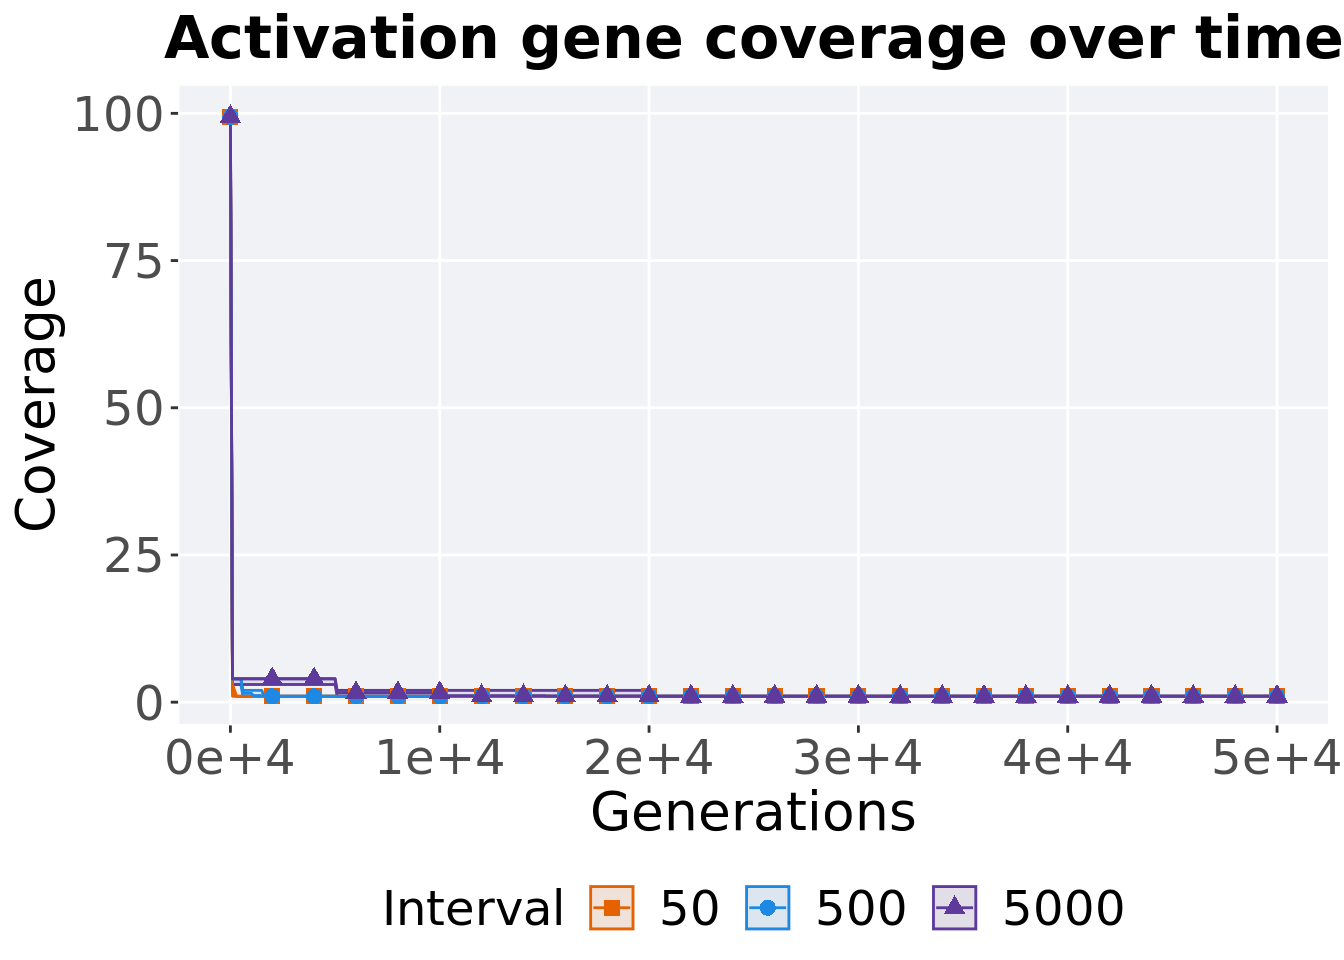
\includegraphics{demo_files/figure-latex/int-con-act-tru-ot-1.pdf}

\hypertarget{end-of-50000-generations-1}{%
\subsubsection{End of 50,000 generations}\label{end-of-50000-generations-1}}

Activation gene coverage in the population at the end of 50,000 generations.

\begin{Shaded}
\begin{Highlighting}[]
\CommentTok{### end of run}
\KeywordTok{filter}\NormalTok{(df_ot, Diagnostic }\OperatorTok{==}\StringTok{ 'CONTRADICTORY_OBJECTIVES'} \OperatorTok{&}\StringTok{ `}\DataTypeTok{Selection}\CharTok{\textbackslash{}n}\DataTypeTok{Scheme}\StringTok{`} \OperatorTok{==}\StringTok{ 'TRUNCATION'} \OperatorTok{&}\StringTok{ }\NormalTok{Generations }\OperatorTok{==}\StringTok{ }\DecValTok{50000}\NormalTok{) }\OperatorTok
\StringTok{  }\KeywordTok{ggplot}\NormalTok{(., }\KeywordTok{aes}\NormalTok{(}\DataTypeTok{x =}\NormalTok{ Interval, }\DataTypeTok{y =}\NormalTok{ pop_act_cov, }\DataTypeTok{color =}\NormalTok{ Interval, }\DataTypeTok{fill =}\NormalTok{ Interval, }\DataTypeTok{shape =}\NormalTok{ Interval)) }\OperatorTok{+}
\StringTok{  }\KeywordTok{geom_flat_violin}\NormalTok{(}\DataTypeTok{position =} \KeywordTok{position_nudge}\NormalTok{(}\DataTypeTok{x =} \FloatTok{.2}\NormalTok{, }\DataTypeTok{y =} \DecValTok{0}\NormalTok{), }\DataTypeTok{scale =} \StringTok{'width'}\NormalTok{, }\DataTypeTok{alpha =} \FloatTok{0.3}\NormalTok{) }\OperatorTok{+}
\StringTok{  }\KeywordTok{geom_point}\NormalTok{(}\DataTypeTok{position =} \KeywordTok{position_jitter}\NormalTok{(}\DataTypeTok{height =} \FloatTok{.05}\NormalTok{, }\DataTypeTok{width =} \FloatTok{.05}\NormalTok{), }\DataTypeTok{size =} \FloatTok{1.5}\NormalTok{, }\DataTypeTok{alpha =} \FloatTok{0.5}\NormalTok{) }\OperatorTok{+}
\StringTok{  }\KeywordTok{geom_boxplot}\NormalTok{(}\DataTypeTok{color =} \StringTok{'black'}\NormalTok{, }\DataTypeTok{width =} \FloatTok{.2}\NormalTok{, }\DataTypeTok{outlier.shape =} \OtherTok{NA}\NormalTok{, }\DataTypeTok{alpha =} \FloatTok{0.0}\NormalTok{) }\OperatorTok{+}
\StringTok{  }\KeywordTok{scale_shape_manual}\NormalTok{(}\DataTypeTok{values=}\NormalTok{SHAPE)}\OperatorTok{+}
\StringTok{  }\KeywordTok{scale_y_continuous}\NormalTok{(}
    \DataTypeTok{name=}\StringTok{"Coverage"}
\NormalTok{  ) }\OperatorTok{+}
\StringTok{  }\KeywordTok{scale_x_discrete}\NormalTok{(}
    \DataTypeTok{name=}\StringTok{"Interval"}
\NormalTok{  ) }\OperatorTok{+}
\StringTok{  }\KeywordTok{scale_colour_manual}\NormalTok{(}\DataTypeTok{values =}\NormalTok{ cb_palette_mi) }\OperatorTok{+}
\StringTok{  }\KeywordTok{scale_fill_manual}\NormalTok{(}\DataTypeTok{values =}\NormalTok{ cb_palette_mi) }\OperatorTok{+}
\StringTok{  }\KeywordTok{ggtitle}\NormalTok{(}\StringTok{'Final activation gene coverage'}\NormalTok{)}\OperatorTok{+}
\StringTok{  }\NormalTok{p_theme }\OperatorTok{+}\StringTok{ }\KeywordTok{coord_flip}\NormalTok{()}
\end{Highlighting}
\end{Shaded}

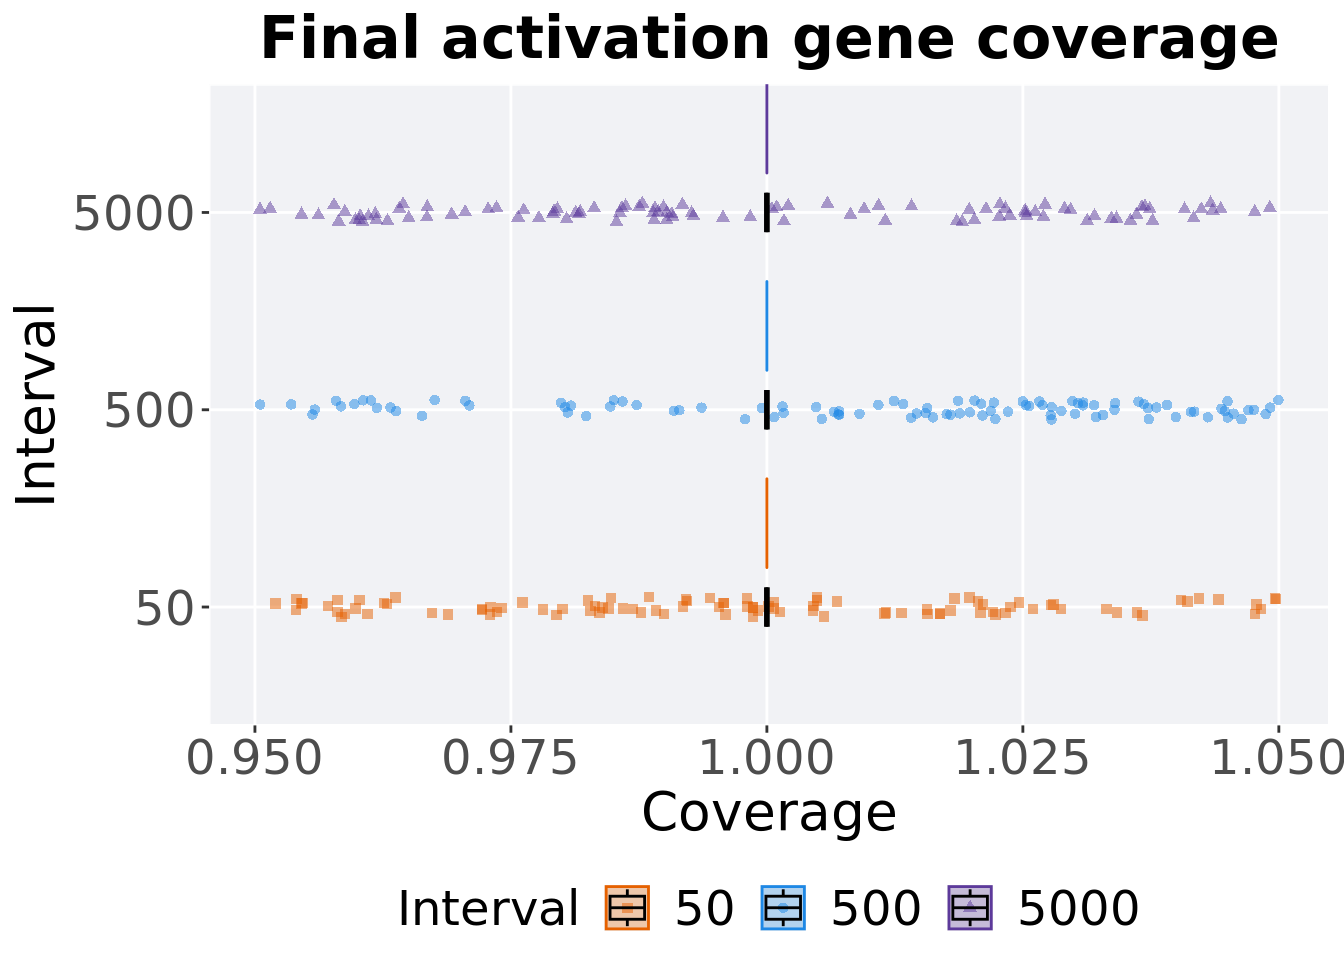
\includegraphics{demo_files/figure-latex/int-con-act-tru-end-1.pdf}

\hypertarget{stats-9}{%
\paragraph{Stats}\label{stats-9}}

Summary statistics for activation gene coverage.

\begin{Shaded}
\begin{Highlighting}[]
\NormalTok{coverage =}\StringTok{ }\KeywordTok{filter}\NormalTok{(df_ot, Diagnostic }\OperatorTok{==}\StringTok{ 'CONTRADICTORY_OBJECTIVES'} \OperatorTok{&}\StringTok{ `}\DataTypeTok{Selection}\CharTok{\textbackslash{}n}\DataTypeTok{Scheme}\StringTok{`} \OperatorTok{==}\StringTok{ 'TRUNCATION'} \OperatorTok{&}\StringTok{ }\NormalTok{Generations }\OperatorTok{==}\StringTok{ }\DecValTok{50000}\NormalTok{)}
\NormalTok{coverage }\OperatorTok
\StringTok{  }\KeywordTok{group_by}\NormalTok{(Interval) }\OperatorTok
\StringTok{  }\NormalTok{dplyr}\OperatorTok{::}\KeywordTok{summarise}\NormalTok{(}
    \DataTypeTok{count =} \KeywordTok{n}\NormalTok{(),}
    \DataTypeTok{na_cnt =} \KeywordTok{sum}\NormalTok{(}\KeywordTok{is.na}\NormalTok{(pop_act_cov)),}
    \DataTypeTok{min =} \KeywordTok{min}\NormalTok{(pop_act_cov, }\DataTypeTok{na.rm =} \OtherTok{TRUE}\NormalTok{),}
    \DataTypeTok{median =} \KeywordTok{median}\NormalTok{(pop_act_cov, }\DataTypeTok{na.rm =} \OtherTok{TRUE}\NormalTok{),}
    \DataTypeTok{mean =} \KeywordTok{mean}\NormalTok{(pop_act_cov, }\DataTypeTok{na.rm =} \OtherTok{TRUE}\NormalTok{),}
    \DataTypeTok{max =} \KeywordTok{max}\NormalTok{(pop_act_cov, }\DataTypeTok{na.rm =} \OtherTok{TRUE}\NormalTok{),}
    \DataTypeTok{IQR =} \KeywordTok{IQR}\NormalTok{(pop_act_cov, }\DataTypeTok{na.rm =} \OtherTok{TRUE}\NormalTok{)}
\NormalTok{  )}
\end{Highlighting}
\end{Shaded}

\begin{verbatim}
## # A tibble: 3 x 8
##   Interval count na_cnt   min median  mean   max   IQR
##   <fct>    <int>  <int> <int>  <dbl> <dbl> <int> <dbl>
## 1 50         100      0     1      1     1     1     0
## 2 500        100      0     1      1     1     1     0
## 3 5000       100      0     1      1     1     1     0
\end{verbatim}

Kruskal--Wallis test provides evidence of difference among activation gene coverage.

\begin{Shaded}
\begin{Highlighting}[]
\KeywordTok{kruskal.test}\NormalTok{(pop_act_cov }\OperatorTok{~}\StringTok{ }\NormalTok{Interval, }\DataTypeTok{data =}\NormalTok{ coverage)}
\end{Highlighting}
\end{Shaded}

\begin{verbatim}
## 
##  Kruskal-Wallis rank sum test
## 
## data:  pop_act_cov by Interval
## Kruskal-Wallis chi-squared = NaN, df = 2, p-value = NA
\end{verbatim}

Results for post-hoc Wilcoxon rank-sum test with a Bonferroni correction on activation gene coverage.

\begin{Shaded}
\begin{Highlighting}[]
\KeywordTok{pairwise.wilcox.test}\NormalTok{(}\DataTypeTok{x =}\NormalTok{ coverage}\OperatorTok{$}\NormalTok{pop_act_cov, }\DataTypeTok{g =}\NormalTok{ coverage}\OperatorTok{$}\NormalTok{Interval, }\DataTypeTok{p.adjust.method =} \StringTok{"bonferroni"}\NormalTok{,}
                     \DataTypeTok{paired =} \OtherTok{FALSE}\NormalTok{, }\DataTypeTok{conf.int =} \OtherTok{FALSE}\NormalTok{, }\DataTypeTok{alternative =} \StringTok{'g'}\NormalTok{)}
\end{Highlighting}
\end{Shaded}

\begin{verbatim}
## 
##  Pairwise comparisons using Wilcoxon rank sum test with continuity correction 
## 
## data:  coverage$pop_act_cov and coverage$Interval 
## 
##      50 500
## 500  1  -  
## 5000 1  1  
## 
## P value adjustment method: bonferroni
\end{verbatim}

\hypertarget{tournament-selection-2}{%
\section{Tournament selection}\label{tournament-selection-2}}

Here we analyze how the different population structures affect tournament selection (size 8) on the contradictory objectives diagnostic.

\hypertarget{satisfactory-trait-coverage-1}{%
\subsection{Satisfactory trait coverage}\label{satisfactory-trait-coverage-1}}

Satisfactory trait coverage analysis.

\hypertarget{coverage-over-time-2}{%
\subsubsection{Coverage over time}\label{coverage-over-time-2}}

Satisfactory trait coverage over time.

\begin{Shaded}
\begin{Highlighting}[]
\NormalTok{lines =}\StringTok{ }\KeywordTok{filter}\NormalTok{(df_ot, Diagnostic }\OperatorTok{==}\StringTok{ 'CONTRADICTORY_OBJECTIVES'} \OperatorTok{&}\StringTok{ `}\DataTypeTok{Selection}\CharTok{\textbackslash{}n}\DataTypeTok{Scheme}\StringTok{`} \OperatorTok{==}\StringTok{ 'TOURNAMENT'}\NormalTok{) }\OperatorTok
\StringTok{  }\KeywordTok{group_by}\NormalTok{(Interval, Generations) }\OperatorTok
\StringTok{  }\NormalTok{dplyr}\OperatorTok{::}\KeywordTok{summarise}\NormalTok{(}
    \DataTypeTok{min =} \KeywordTok{min}\NormalTok{(pop_sat_cov),}
    \DataTypeTok{mean =} \KeywordTok{mean}\NormalTok{(pop_sat_cov),}
    \DataTypeTok{max =} \KeywordTok{max}\NormalTok{(pop_sat_cov)}
\NormalTok{  )}
\end{Highlighting}
\end{Shaded}

\begin{verbatim}
## `summarise()` has grouped output by 'Interval'. You can override using the
## `.groups` argument.
\end{verbatim}

\begin{Shaded}
\begin{Highlighting}[]
\KeywordTok{ggplot}\NormalTok{(lines, }\KeywordTok{aes}\NormalTok{(}\DataTypeTok{x=}\NormalTok{Generations, }\DataTypeTok{y=}\NormalTok{mean, }\DataTypeTok{group =}\NormalTok{ Interval, }\DataTypeTok{fill =}\NormalTok{ Interval, }\DataTypeTok{color =}\NormalTok{ Interval, }\DataTypeTok{shape =}\NormalTok{ Interval)) }\OperatorTok{+}
\StringTok{  }\KeywordTok{geom_ribbon}\NormalTok{(}\KeywordTok{aes}\NormalTok{(}\DataTypeTok{ymin =}\NormalTok{ min, }\DataTypeTok{ymax =}\NormalTok{ max), }\DataTypeTok{alpha =} \FloatTok{0.1}\NormalTok{) }\OperatorTok{+}
\StringTok{  }\KeywordTok{geom_line}\NormalTok{(}\DataTypeTok{size =} \FloatTok{0.5}\NormalTok{) }\OperatorTok{+}
\StringTok{  }\KeywordTok{geom_point}\NormalTok{(}\DataTypeTok{data =} \KeywordTok{filter}\NormalTok{(lines, Generations }\OperatorTok\StringTok{ }\DecValTok{2000} \OperatorTok{==}\StringTok{ }\DecValTok{0}\NormalTok{), }\DataTypeTok{size =} \FloatTok{1.5}\NormalTok{, }\DataTypeTok{stroke =} \FloatTok{2.0}\NormalTok{, }\DataTypeTok{alpha =} \FloatTok{1.0}\NormalTok{) }\OperatorTok{+}
\StringTok{  }\KeywordTok{scale_y_continuous}\NormalTok{(}
    \DataTypeTok{name=}\StringTok{"Coverage"}
\NormalTok{  ) }\OperatorTok{+}
\StringTok{  }\KeywordTok{scale_x_continuous}\NormalTok{(}
    \DataTypeTok{name=}\StringTok{"Generations"}\NormalTok{,}
    \DataTypeTok{limits=}\KeywordTok{c}\NormalTok{(}\DecValTok{0}\NormalTok{, }\DecValTok{50000}\NormalTok{),}
    \DataTypeTok{breaks=}\KeywordTok{c}\NormalTok{(}\DecValTok{0}\NormalTok{, }\DecValTok{10000}\NormalTok{, }\DecValTok{20000}\NormalTok{, }\DecValTok{30000}\NormalTok{, }\DecValTok{40000}\NormalTok{, }\DecValTok{50000}\NormalTok{),}
    \DataTypeTok{labels=}\KeywordTok{c}\NormalTok{(}\StringTok{"0e+4"}\NormalTok{, }\StringTok{"1e+4"}\NormalTok{, }\StringTok{"2e+4"}\NormalTok{, }\StringTok{"3e+4"}\NormalTok{, }\StringTok{"4e+4"}\NormalTok{, }\StringTok{"5e+4"}\NormalTok{)}

\NormalTok{  ) }\OperatorTok{+}
\StringTok{  }\KeywordTok{scale_shape_manual}\NormalTok{(}\DataTypeTok{values=}\NormalTok{SHAPE)}\OperatorTok{+}
\StringTok{  }\KeywordTok{scale_colour_manual}\NormalTok{(}\DataTypeTok{values =}\NormalTok{ cb_palette_mi) }\OperatorTok{+}
\StringTok{  }\KeywordTok{scale_fill_manual}\NormalTok{(}\DataTypeTok{values =}\NormalTok{ cb_palette_mi) }\OperatorTok{+}
\StringTok{  }\KeywordTok{ggtitle}\NormalTok{(}\StringTok{'Satisfactory trait coverage over time'}\NormalTok{)}\OperatorTok{+}
\StringTok{  }\NormalTok{p_theme}
\end{Highlighting}
\end{Shaded}

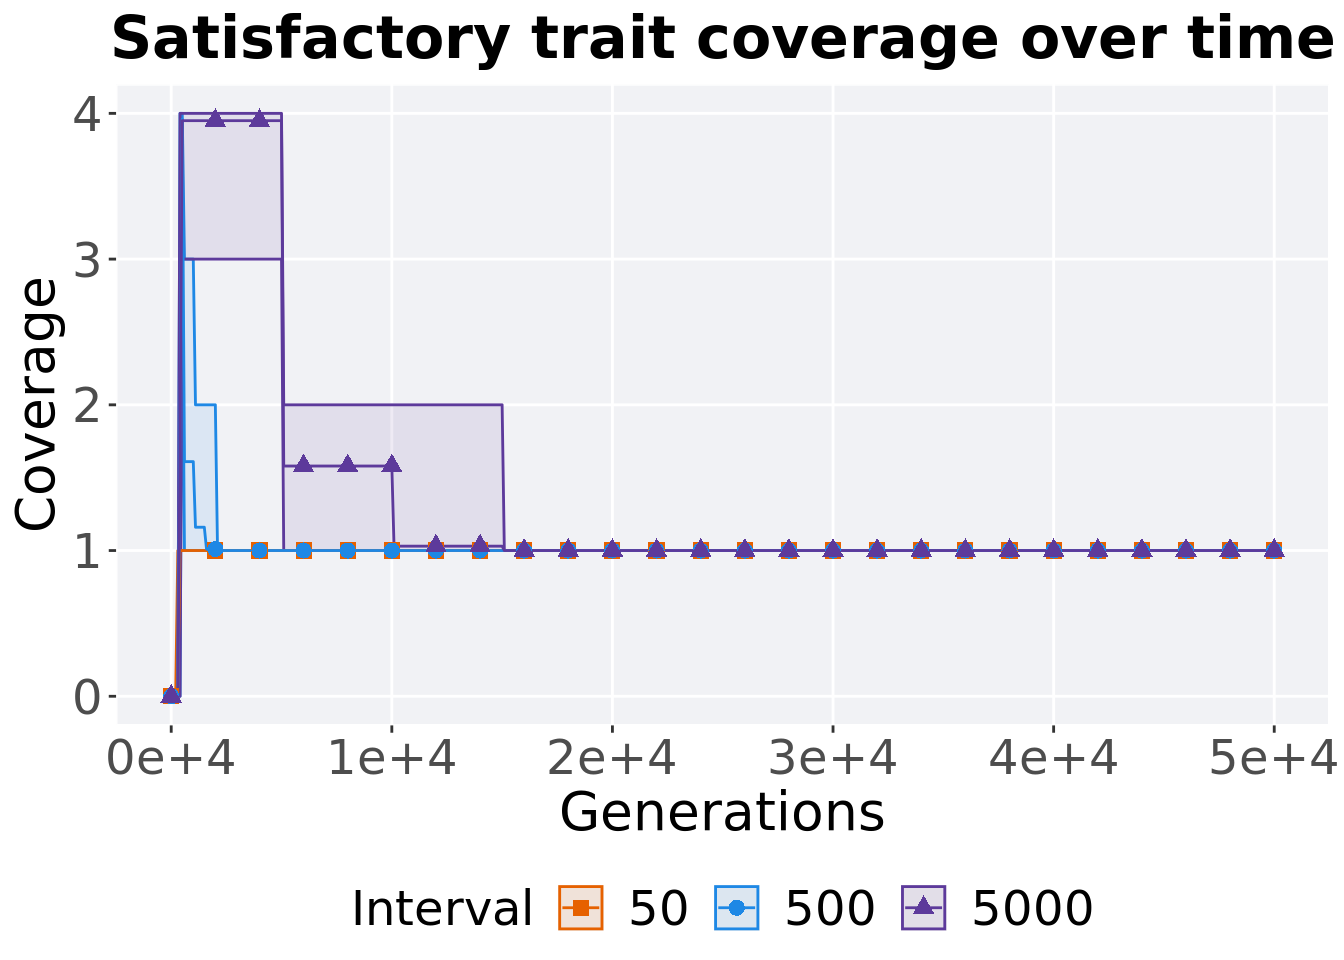
\includegraphics{demo_files/figure-latex/int-con-sat-tor-ot-1.pdf}

\hypertarget{best-coverage-throughout-1}{%
\subsubsection{Best coverage throughout}\label{best-coverage-throughout-1}}

Best satisfactory trait coverage throughout 50,000 generations.

\begin{Shaded}
\begin{Highlighting}[]
\CommentTok{### best satisfactory trait coverage throughout}
\KeywordTok{filter}\NormalTok{(df_best, Diagnostic }\OperatorTok{==}\StringTok{ 'CONTRADICTORY_OBJECTIVES'} \OperatorTok{&}\StringTok{ `}\DataTypeTok{Selection}\CharTok{\textbackslash{}n}\DataTypeTok{Scheme}\StringTok{`} \OperatorTok{==}\StringTok{ 'TOURNAMENT'} \OperatorTok{&}\StringTok{ }\NormalTok{VAR }\OperatorTok{==}\StringTok{ 'pop_sat_cov'}\NormalTok{) }\OperatorTok
\StringTok{  }\KeywordTok{ggplot}\NormalTok{(., }\KeywordTok{aes}\NormalTok{(}\DataTypeTok{x =}\NormalTok{ Interval, }\DataTypeTok{y =}\NormalTok{ VAL, }\DataTypeTok{color =}\NormalTok{ Interval, }\DataTypeTok{fill =}\NormalTok{ Interval, }\DataTypeTok{shape =}\NormalTok{ Interval)) }\OperatorTok{+}
\StringTok{  }\KeywordTok{geom_flat_violin}\NormalTok{(}\DataTypeTok{position =} \KeywordTok{position_nudge}\NormalTok{(}\DataTypeTok{x =} \FloatTok{.2}\NormalTok{, }\DataTypeTok{y =} \DecValTok{0}\NormalTok{), }\DataTypeTok{scale =} \StringTok{'width'}\NormalTok{, }\DataTypeTok{alpha =} \FloatTok{0.2}\NormalTok{) }\OperatorTok{+}
\StringTok{  }\KeywordTok{geom_point}\NormalTok{(}\DataTypeTok{position =} \KeywordTok{position_jitter}\NormalTok{(}\DataTypeTok{height =} \FloatTok{.05}\NormalTok{, }\DataTypeTok{width =} \FloatTok{.05}\NormalTok{), }\DataTypeTok{size =} \FloatTok{1.5}\NormalTok{, }\DataTypeTok{alpha =} \FloatTok{1.0}\NormalTok{) }\OperatorTok{+}
\StringTok{  }\KeywordTok{geom_boxplot}\NormalTok{(}\DataTypeTok{color =} \StringTok{'black'}\NormalTok{, }\DataTypeTok{width =} \FloatTok{.2}\NormalTok{, }\DataTypeTok{outlier.shape =} \OtherTok{NA}\NormalTok{, }\DataTypeTok{alpha =} \FloatTok{0.0}\NormalTok{) }\OperatorTok{+}
\StringTok{  }\KeywordTok{scale_y_continuous}\NormalTok{(}
    \DataTypeTok{name=}\StringTok{"coverage"}
\NormalTok{  ) }\OperatorTok{+}
\StringTok{  }\KeywordTok{scale_x_discrete}\NormalTok{(}
    \DataTypeTok{name=}\StringTok{"Interval"}
\NormalTok{  )}\OperatorTok{+}
\StringTok{  }\KeywordTok{scale_shape_manual}\NormalTok{(}\DataTypeTok{values=}\NormalTok{SHAPE)}\OperatorTok{+}
\StringTok{  }\KeywordTok{scale_colour_manual}\NormalTok{(}\DataTypeTok{values =}\NormalTok{ cb_palette_mi, ) }\OperatorTok{+}
\StringTok{  }\KeywordTok{scale_fill_manual}\NormalTok{(}\DataTypeTok{values =}\NormalTok{ cb_palette_mi) }\OperatorTok{+}
\StringTok{  }\KeywordTok{ggtitle}\NormalTok{(}\StringTok{'Best satisfactory trait coverage'}\NormalTok{)}\OperatorTok{+}
\StringTok{  }\NormalTok{p_theme }\OperatorTok{+}\StringTok{ }\KeywordTok{coord_flip}\NormalTok{()}
\end{Highlighting}
\end{Shaded}

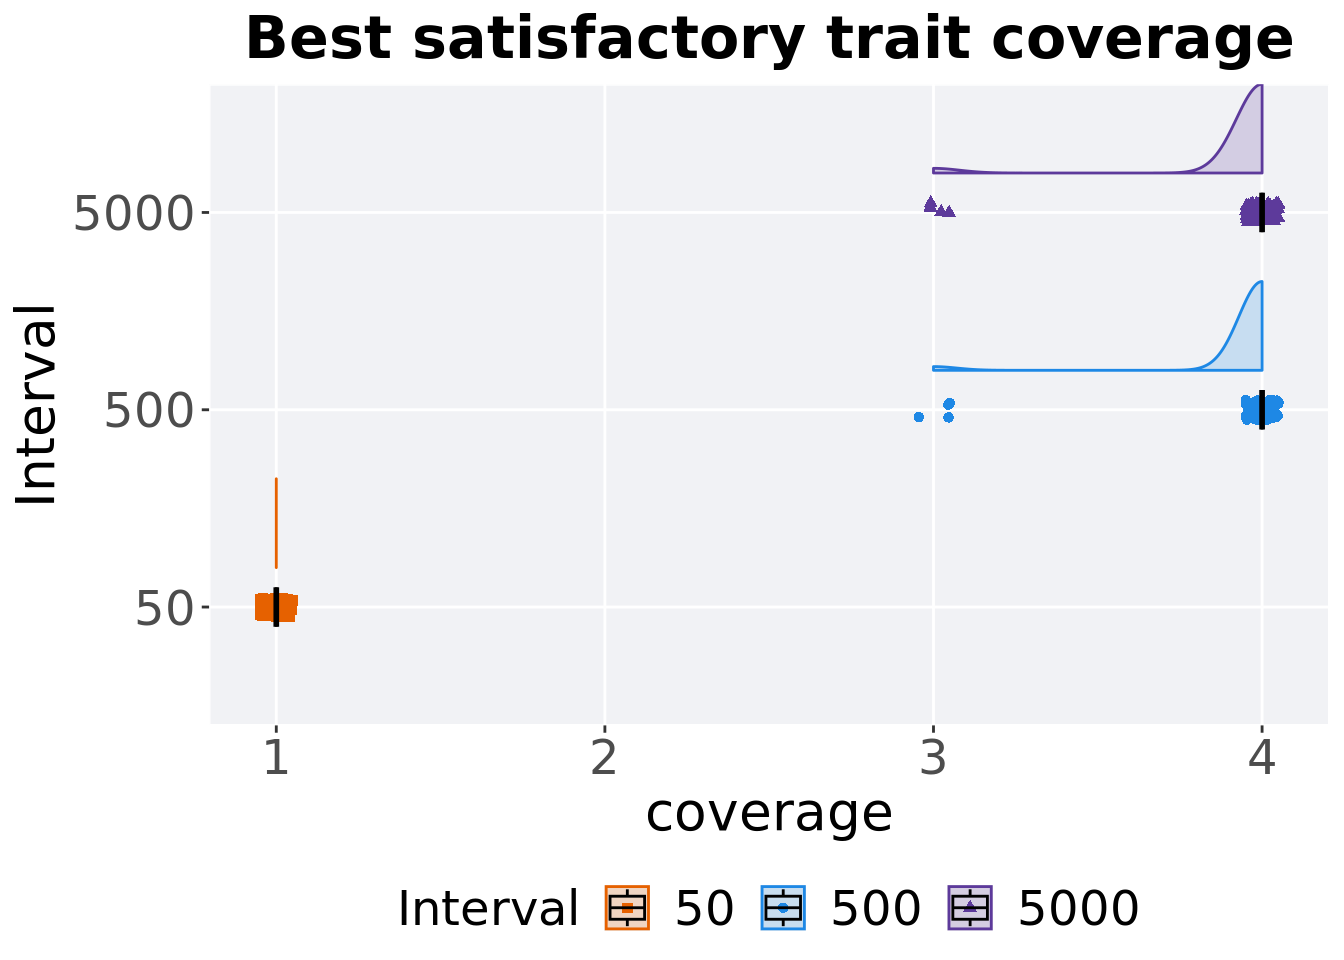
\includegraphics{demo_files/figure-latex/int-con-sat-tor-bst-1.pdf}

\hypertarget{stats-10}{%
\paragraph{Stats}\label{stats-10}}

Summary statistics for the best satisfactory trait coverage.

\begin{Shaded}
\begin{Highlighting}[]
\CommentTok{### best}
\NormalTok{coverage =}\StringTok{ }\KeywordTok{filter}\NormalTok{(df_best, Diagnostic }\OperatorTok{==}\StringTok{ 'CONTRADICTORY_OBJECTIVES'} \OperatorTok{&}\StringTok{ `}\DataTypeTok{Selection}\CharTok{\textbackslash{}n}\DataTypeTok{Scheme}\StringTok{`} \OperatorTok{==}\StringTok{ 'TOURNAMENT'} \OperatorTok{&}\StringTok{ }\NormalTok{VAR }\OperatorTok{==}\StringTok{ 'pop_sat_cov'}\NormalTok{)}
\NormalTok{coverage }\OperatorTok
\StringTok{  }\KeywordTok{group_by}\NormalTok{(Interval) }\OperatorTok
\StringTok{  }\NormalTok{dplyr}\OperatorTok{::}\KeywordTok{summarise}\NormalTok{(}
    \DataTypeTok{count =} \KeywordTok{n}\NormalTok{(),}
    \DataTypeTok{na_cnt =} \KeywordTok{sum}\NormalTok{(}\KeywordTok{is.na}\NormalTok{(VAL)),}
    \DataTypeTok{min =} \KeywordTok{min}\NormalTok{(VAL, }\DataTypeTok{na.rm =} \OtherTok{TRUE}\NormalTok{),}
    \DataTypeTok{median =} \KeywordTok{median}\NormalTok{(VAL, }\DataTypeTok{na.rm =} \OtherTok{TRUE}\NormalTok{),}
    \DataTypeTok{mean =} \KeywordTok{mean}\NormalTok{(VAL, }\DataTypeTok{na.rm =} \OtherTok{TRUE}\NormalTok{),}
    \DataTypeTok{max =} \KeywordTok{max}\NormalTok{(VAL, }\DataTypeTok{na.rm =} \OtherTok{TRUE}\NormalTok{),}
    \DataTypeTok{IQR =} \KeywordTok{IQR}\NormalTok{(VAL, }\DataTypeTok{na.rm =} \OtherTok{TRUE}\NormalTok{)}
\NormalTok{  )}
\end{Highlighting}
\end{Shaded}

\begin{verbatim}
## # A tibble: 3 x 8
##   Interval count na_cnt   min median  mean   max   IQR
##   <fct>    <int>  <int> <dbl>  <dbl> <dbl> <dbl> <dbl>
## 1 50         100      0     1      1  1        1     0
## 2 500        100      0     3      4  3.96     4     0
## 3 5000       100      0     3      4  3.95     4     0
\end{verbatim}

Kruskal--Wallis test provides evidence of difference among satisfactory trait coverage.

\begin{Shaded}
\begin{Highlighting}[]
\KeywordTok{kruskal.test}\NormalTok{(VAL }\OperatorTok{~}\StringTok{ }\NormalTok{Interval, }\DataTypeTok{data =}\NormalTok{ coverage)}
\end{Highlighting}
\end{Shaded}

\begin{verbatim}
## 
##  Kruskal-Wallis rank sum test
## 
## data:  VAL by Interval
## Kruskal-Wallis chi-squared = 282.81, df = 2, p-value < 2.2e-16
\end{verbatim}

Results for post-hoc Wilcoxon rank-sum test with a Bonferroni correction on satisfactory trait coverage.

\begin{Shaded}
\begin{Highlighting}[]
\KeywordTok{pairwise.wilcox.test}\NormalTok{(}\DataTypeTok{x =}\NormalTok{ coverage}\OperatorTok{$}\NormalTok{VAL, }\DataTypeTok{g =}\NormalTok{ coverage}\OperatorTok{$}\NormalTok{Interval, }\DataTypeTok{p.adjust.method =} \StringTok{"bonferroni"}\NormalTok{,}
                     \DataTypeTok{paired =} \OtherTok{FALSE}\NormalTok{, }\DataTypeTok{conf.int =} \OtherTok{FALSE}\NormalTok{, }\DataTypeTok{alternative =} \StringTok{'g'}\NormalTok{)}
\end{Highlighting}
\end{Shaded}

\begin{verbatim}
## 
##  Pairwise comparisons using Wilcoxon rank sum test with continuity correction 
## 
## data:  coverage$VAL and coverage$Interval 
## 
##      50     500
## 500  <2e-16 -  
## 5000 <2e-16 1  
## 
## P value adjustment method: bonferroni
\end{verbatim}

\hypertarget{end-of-50000-generations-2}{%
\subsubsection{End of 50,000 generations}\label{end-of-50000-generations-2}}

Satisfactory trait coverage in the population at the end of 50,000 generations.

\begin{Shaded}
\begin{Highlighting}[]
\CommentTok{### end of run}
\KeywordTok{filter}\NormalTok{(df_ot, Diagnostic }\OperatorTok{==}\StringTok{ 'CONTRADICTORY_OBJECTIVES'} \OperatorTok{&}\StringTok{ `}\DataTypeTok{Selection}\CharTok{\textbackslash{}n}\DataTypeTok{Scheme}\StringTok{`} \OperatorTok{==}\StringTok{ 'TOURNAMENT'} \OperatorTok{&}\StringTok{ }\NormalTok{Generations }\OperatorTok{==}\StringTok{ }\DecValTok{50000}\NormalTok{) }\OperatorTok
\StringTok{  }\KeywordTok{ggplot}\NormalTok{(., }\KeywordTok{aes}\NormalTok{(}\DataTypeTok{x =}\NormalTok{ Interval, }\DataTypeTok{y =}\NormalTok{ pop_sat_cov, }\DataTypeTok{color =}\NormalTok{ Interval, }\DataTypeTok{fill =}\NormalTok{ Interval, }\DataTypeTok{shape =}\NormalTok{ Interval)) }\OperatorTok{+}
\StringTok{  }\KeywordTok{geom_flat_violin}\NormalTok{(}\DataTypeTok{position =} \KeywordTok{position_nudge}\NormalTok{(}\DataTypeTok{x =} \FloatTok{.2}\NormalTok{, }\DataTypeTok{y =} \DecValTok{0}\NormalTok{), }\DataTypeTok{scale =} \StringTok{'width'}\NormalTok{, }\DataTypeTok{alpha =} \FloatTok{0.3}\NormalTok{) }\OperatorTok{+}
\StringTok{  }\KeywordTok{geom_point}\NormalTok{(}\DataTypeTok{position =} \KeywordTok{position_jitter}\NormalTok{(}\DataTypeTok{height =} \FloatTok{.05}\NormalTok{, }\DataTypeTok{width =} \FloatTok{.05}\NormalTok{), }\DataTypeTok{size =} \FloatTok{1.5}\NormalTok{, }\DataTypeTok{alpha =} \FloatTok{0.5}\NormalTok{) }\OperatorTok{+}
\StringTok{  }\KeywordTok{geom_boxplot}\NormalTok{(}\DataTypeTok{color =} \StringTok{'black'}\NormalTok{, }\DataTypeTok{width =} \FloatTok{.2}\NormalTok{, }\DataTypeTok{outlier.shape =} \OtherTok{NA}\NormalTok{, }\DataTypeTok{alpha =} \FloatTok{0.0}\NormalTok{) }\OperatorTok{+}
\StringTok{  }\KeywordTok{scale_shape_manual}\NormalTok{(}\DataTypeTok{values=}\NormalTok{SHAPE)}\OperatorTok{+}
\StringTok{  }\KeywordTok{scale_y_continuous}\NormalTok{(}
    \DataTypeTok{name=}\StringTok{"Coverage"}
\NormalTok{  ) }\OperatorTok{+}
\StringTok{  }\KeywordTok{scale_x_discrete}\NormalTok{(}
    \DataTypeTok{name=}\StringTok{"Interval"}
\NormalTok{  ) }\OperatorTok{+}
\StringTok{  }\KeywordTok{scale_colour_manual}\NormalTok{(}\DataTypeTok{values =}\NormalTok{ cb_palette_mi) }\OperatorTok{+}
\StringTok{  }\KeywordTok{scale_fill_manual}\NormalTok{(}\DataTypeTok{values =}\NormalTok{ cb_palette_mi) }\OperatorTok{+}
\StringTok{  }\KeywordTok{ggtitle}\NormalTok{(}\StringTok{'Final satisfactory trait coverage'}\NormalTok{)}\OperatorTok{+}
\StringTok{  }\NormalTok{p_theme }\OperatorTok{+}\StringTok{ }\KeywordTok{coord_flip}\NormalTok{()}
\end{Highlighting}
\end{Shaded}

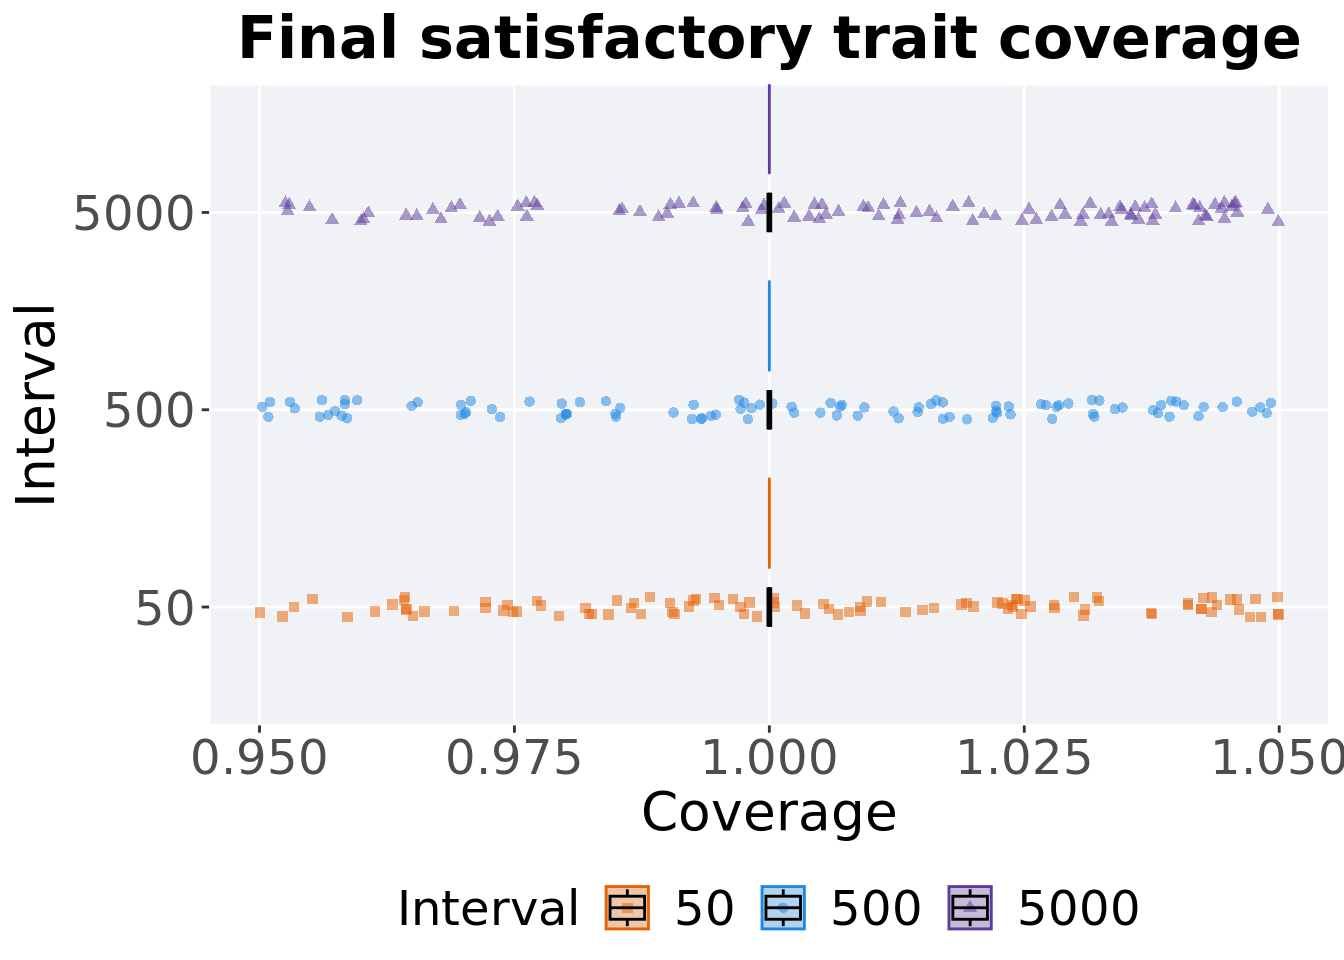
\includegraphics{demo_files/figure-latex/int-con-sat-tor-end-1.pdf}

\hypertarget{stats-11}{%
\paragraph{Stats}\label{stats-11}}

Summary statistics for satisfactory trait coverage in the population at the end of 50,000 generations.

\begin{Shaded}
\begin{Highlighting}[]
\CommentTok{### end of run}
\NormalTok{coverage =}\StringTok{ }\KeywordTok{filter}\NormalTok{(df_ot, Diagnostic }\OperatorTok{==}\StringTok{ 'CONTRADICTORY_OBJECTIVES'} \OperatorTok{&}\StringTok{ `}\DataTypeTok{Selection}\CharTok{\textbackslash{}n}\DataTypeTok{Scheme}\StringTok{`} \OperatorTok{==}\StringTok{ 'TOURNAMENT'} \OperatorTok{&}\StringTok{ }\NormalTok{Generations }\OperatorTok{==}\StringTok{ }\DecValTok{50000}\NormalTok{)}
\NormalTok{coverage }\OperatorTok
\StringTok{  }\KeywordTok{group_by}\NormalTok{(Interval) }\OperatorTok
\StringTok{  }\NormalTok{dplyr}\OperatorTok{::}\KeywordTok{summarise}\NormalTok{(}
    \DataTypeTok{count =} \KeywordTok{n}\NormalTok{(),}
    \DataTypeTok{na_cnt =} \KeywordTok{sum}\NormalTok{(}\KeywordTok{is.na}\NormalTok{(pop_sat_cov)),}
    \DataTypeTok{min =} \KeywordTok{min}\NormalTok{(pop_sat_cov, }\DataTypeTok{na.rm =} \OtherTok{TRUE}\NormalTok{),}
    \DataTypeTok{median =} \KeywordTok{median}\NormalTok{(pop_sat_cov, }\DataTypeTok{na.rm =} \OtherTok{TRUE}\NormalTok{),}
    \DataTypeTok{mean =} \KeywordTok{mean}\NormalTok{(pop_sat_cov, }\DataTypeTok{na.rm =} \OtherTok{TRUE}\NormalTok{),}
    \DataTypeTok{max =} \KeywordTok{max}\NormalTok{(pop_sat_cov, }\DataTypeTok{na.rm =} \OtherTok{TRUE}\NormalTok{),}
    \DataTypeTok{IQR =} \KeywordTok{IQR}\NormalTok{(pop_sat_cov, }\DataTypeTok{na.rm =} \OtherTok{TRUE}\NormalTok{)}
\NormalTok{  )}
\end{Highlighting}
\end{Shaded}

\begin{verbatim}
## # A tibble: 3 x 8
##   Interval count na_cnt   min median  mean   max   IQR
##   <fct>    <int>  <int> <int>  <dbl> <dbl> <int> <dbl>
## 1 50         100      0     1      1     1     1     0
## 2 500        100      0     1      1     1     1     0
## 3 5000       100      0     1      1     1     1     0
\end{verbatim}

Kruskal--Wallis test provides evidence of difference among satisfactory trait coverage in the population at the end of 50,000 generations.

\begin{Shaded}
\begin{Highlighting}[]
\KeywordTok{kruskal.test}\NormalTok{(pop_sat_cov }\OperatorTok{~}\StringTok{ }\NormalTok{Interval, }\DataTypeTok{data =}\NormalTok{ coverage)}
\end{Highlighting}
\end{Shaded}

\begin{verbatim}
## 
##  Kruskal-Wallis rank sum test
## 
## data:  pop_sat_cov by Interval
## Kruskal-Wallis chi-squared = NaN, df = 2, p-value = NA
\end{verbatim}

Results for post-hoc Wilcoxon rank-sum test with a Bonferroni correction on satisfactory trait coverage in the population at the end of 50,000 generations.

\begin{Shaded}
\begin{Highlighting}[]
\KeywordTok{pairwise.wilcox.test}\NormalTok{(}\DataTypeTok{x =}\NormalTok{ coverage}\OperatorTok{$}\NormalTok{pop_sat_cov, }\DataTypeTok{g =}\NormalTok{ coverage}\OperatorTok{$}\NormalTok{Interval, }\DataTypeTok{p.adjust.method =} \StringTok{"bonferroni"}\NormalTok{,}
                     \DataTypeTok{paired =} \OtherTok{FALSE}\NormalTok{, }\DataTypeTok{conf.int =} \OtherTok{FALSE}\NormalTok{, }\DataTypeTok{alternative =} \StringTok{'g'}\NormalTok{)}
\end{Highlighting}
\end{Shaded}

\begin{verbatim}
## 
##  Pairwise comparisons using Wilcoxon rank sum test with continuity correction 
## 
## data:  coverage$pop_sat_cov and coverage$Interval 
## 
##      50 500
## 500  1  -  
## 5000 1  1  
## 
## P value adjustment method: bonferroni
\end{verbatim}

\hypertarget{activation-gene-coverage-1}{%
\subsection{Activation gene coverage}\label{activation-gene-coverage-1}}

Activation gene coverage analysis.

\hypertarget{coverage-over-time-3}{%
\subsubsection{Coverage over time}\label{coverage-over-time-3}}

Activation gene coverage over time.

\begin{Shaded}
\begin{Highlighting}[]
\CommentTok{# data for lines and shading on plots}
\NormalTok{lines =}\StringTok{ }\KeywordTok{filter}\NormalTok{(df_ot, Diagnostic }\OperatorTok{==}\StringTok{ 'CONTRADICTORY_OBJECTIVES'} \OperatorTok{&}\StringTok{ `}\DataTypeTok{Selection}\CharTok{\textbackslash{}n}\DataTypeTok{Scheme}\StringTok{`} \OperatorTok{==}\StringTok{ 'TOURNAMENT'}\NormalTok{) }\OperatorTok
\StringTok{  }\KeywordTok{group_by}\NormalTok{(Interval, Generations) }\OperatorTok
\StringTok{  }\NormalTok{dplyr}\OperatorTok{::}\KeywordTok{summarise}\NormalTok{(}
    \DataTypeTok{min =} \KeywordTok{min}\NormalTok{(pop_act_cov),}
    \DataTypeTok{mean =} \KeywordTok{mean}\NormalTok{(pop_act_cov),}
    \DataTypeTok{max =} \KeywordTok{max}\NormalTok{(pop_act_cov)}
\NormalTok{  )}
\end{Highlighting}
\end{Shaded}

\begin{verbatim}
## `summarise()` has grouped output by 'Interval'. You can override using the
## `.groups` argument.
\end{verbatim}

\begin{Shaded}
\begin{Highlighting}[]
\KeywordTok{ggplot}\NormalTok{(lines, }\KeywordTok{aes}\NormalTok{(}\DataTypeTok{x=}\NormalTok{Generations, }\DataTypeTok{y=}\NormalTok{mean, }\DataTypeTok{group =}\NormalTok{ Interval, }\DataTypeTok{fill =}\NormalTok{ Interval, }\DataTypeTok{color =}\NormalTok{ Interval, }\DataTypeTok{shape =}\NormalTok{ Interval)) }\OperatorTok{+}
\StringTok{  }\KeywordTok{geom_ribbon}\NormalTok{(}\KeywordTok{aes}\NormalTok{(}\DataTypeTok{ymin =}\NormalTok{ min, }\DataTypeTok{ymax =}\NormalTok{ max), }\DataTypeTok{alpha =} \FloatTok{0.1}\NormalTok{) }\OperatorTok{+}
\StringTok{  }\KeywordTok{geom_line}\NormalTok{(}\DataTypeTok{size =} \FloatTok{0.5}\NormalTok{) }\OperatorTok{+}
\StringTok{  }\KeywordTok{geom_point}\NormalTok{(}\DataTypeTok{data =} \KeywordTok{filter}\NormalTok{(lines, Generations }\OperatorTok\StringTok{ }\DecValTok{2000} \OperatorTok{==}\StringTok{ }\DecValTok{0}\NormalTok{), }\DataTypeTok{size =} \FloatTok{1.5}\NormalTok{, }\DataTypeTok{stroke =} \FloatTok{2.0}\NormalTok{, }\DataTypeTok{alpha =} \FloatTok{1.0}\NormalTok{) }\OperatorTok{+}
\StringTok{  }\KeywordTok{scale_y_continuous}\NormalTok{(}
    \DataTypeTok{name=}\StringTok{"Coverage"}
\NormalTok{  ) }\OperatorTok{+}
\StringTok{  }\KeywordTok{scale_x_continuous}\NormalTok{(}
    \DataTypeTok{name=}\StringTok{"Generations"}\NormalTok{,}
    \DataTypeTok{limits=}\KeywordTok{c}\NormalTok{(}\DecValTok{0}\NormalTok{, }\DecValTok{50000}\NormalTok{),}
    \DataTypeTok{breaks=}\KeywordTok{c}\NormalTok{(}\DecValTok{0}\NormalTok{, }\DecValTok{10000}\NormalTok{, }\DecValTok{20000}\NormalTok{, }\DecValTok{30000}\NormalTok{, }\DecValTok{40000}\NormalTok{, }\DecValTok{50000}\NormalTok{),}
    \DataTypeTok{labels=}\KeywordTok{c}\NormalTok{(}\StringTok{"0e+4"}\NormalTok{, }\StringTok{"1e+4"}\NormalTok{, }\StringTok{"2e+4"}\NormalTok{, }\StringTok{"3e+4"}\NormalTok{, }\StringTok{"4e+4"}\NormalTok{, }\StringTok{"5e+4"}\NormalTok{)}

\NormalTok{  ) }\OperatorTok{+}
\StringTok{  }\KeywordTok{scale_shape_manual}\NormalTok{(}\DataTypeTok{values=}\NormalTok{SHAPE)}\OperatorTok{+}
\StringTok{  }\KeywordTok{scale_colour_manual}\NormalTok{(}\DataTypeTok{values =}\NormalTok{ cb_palette_mi) }\OperatorTok{+}
\StringTok{  }\KeywordTok{scale_fill_manual}\NormalTok{(}\DataTypeTok{values =}\NormalTok{ cb_palette_mi) }\OperatorTok{+}
\StringTok{  }\KeywordTok{ggtitle}\NormalTok{(}\StringTok{'Activation gene coverage over time'}\NormalTok{)}\OperatorTok{+}
\StringTok{  }\NormalTok{p_theme}
\end{Highlighting}
\end{Shaded}

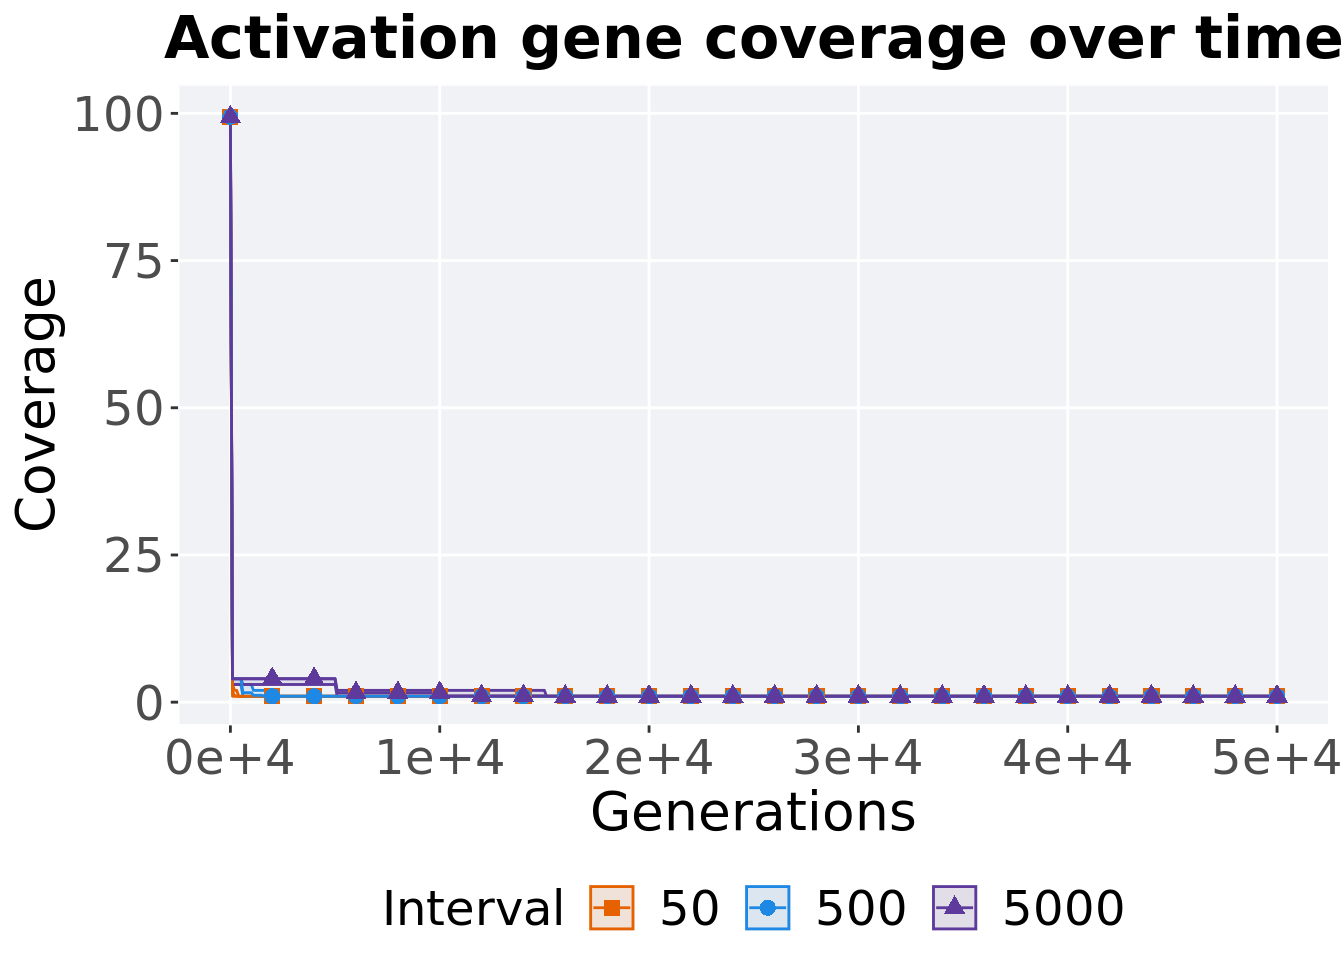
\includegraphics{demo_files/figure-latex/int-con-act-tor-ot-1.pdf}

\hypertarget{end-of-50000-generations-3}{%
\subsubsection{End of 50,000 generations}\label{end-of-50000-generations-3}}

Activation gene coverage in the population at the end of 50,000 generations.

\begin{Shaded}
\begin{Highlighting}[]
\CommentTok{### end of run}
\KeywordTok{filter}\NormalTok{(df_ot, Diagnostic }\OperatorTok{==}\StringTok{ 'CONTRADICTORY_OBJECTIVES'} \OperatorTok{&}\StringTok{ `}\DataTypeTok{Selection}\CharTok{\textbackslash{}n}\DataTypeTok{Scheme}\StringTok{`} \OperatorTok{==}\StringTok{ 'TOURNAMENT'} \OperatorTok{&}\StringTok{ }\NormalTok{Generations }\OperatorTok{==}\StringTok{ }\DecValTok{50000}\NormalTok{) }\OperatorTok
\StringTok{  }\KeywordTok{ggplot}\NormalTok{(., }\KeywordTok{aes}\NormalTok{(}\DataTypeTok{x =}\NormalTok{ Interval, }\DataTypeTok{y =}\NormalTok{ pop_act_cov, }\DataTypeTok{color =}\NormalTok{ Interval, }\DataTypeTok{fill =}\NormalTok{ Interval, }\DataTypeTok{shape =}\NormalTok{ Interval)) }\OperatorTok{+}
\StringTok{  }\KeywordTok{geom_flat_violin}\NormalTok{(}\DataTypeTok{position =} \KeywordTok{position_nudge}\NormalTok{(}\DataTypeTok{x =} \FloatTok{.2}\NormalTok{, }\DataTypeTok{y =} \DecValTok{0}\NormalTok{), }\DataTypeTok{scale =} \StringTok{'width'}\NormalTok{, }\DataTypeTok{alpha =} \FloatTok{0.3}\NormalTok{) }\OperatorTok{+}
\StringTok{  }\KeywordTok{geom_point}\NormalTok{(}\DataTypeTok{position =} \KeywordTok{position_jitter}\NormalTok{(}\DataTypeTok{height =} \FloatTok{.05}\NormalTok{, }\DataTypeTok{width =} \FloatTok{.05}\NormalTok{), }\DataTypeTok{size =} \FloatTok{1.5}\NormalTok{, }\DataTypeTok{alpha =} \FloatTok{0.5}\NormalTok{) }\OperatorTok{+}
\StringTok{  }\KeywordTok{geom_boxplot}\NormalTok{(}\DataTypeTok{color =} \StringTok{'black'}\NormalTok{, }\DataTypeTok{width =} \FloatTok{.2}\NormalTok{, }\DataTypeTok{outlier.shape =} \OtherTok{NA}\NormalTok{, }\DataTypeTok{alpha =} \FloatTok{0.0}\NormalTok{) }\OperatorTok{+}
\StringTok{  }\KeywordTok{scale_shape_manual}\NormalTok{(}\DataTypeTok{values=}\NormalTok{SHAPE)}\OperatorTok{+}
\StringTok{  }\KeywordTok{scale_y_continuous}\NormalTok{(}
    \DataTypeTok{name=}\StringTok{"Coverage"}
\NormalTok{  ) }\OperatorTok{+}
\StringTok{  }\KeywordTok{scale_x_discrete}\NormalTok{(}
    \DataTypeTok{name=}\StringTok{"Interval"}
\NormalTok{  ) }\OperatorTok{+}
\StringTok{  }\KeywordTok{scale_colour_manual}\NormalTok{(}\DataTypeTok{values =}\NormalTok{ cb_palette_mi) }\OperatorTok{+}
\StringTok{  }\KeywordTok{scale_fill_manual}\NormalTok{(}\DataTypeTok{values =}\NormalTok{ cb_palette_mi) }\OperatorTok{+}
\StringTok{  }\KeywordTok{ggtitle}\NormalTok{(}\StringTok{'Final activation gene coverage'}\NormalTok{)}\OperatorTok{+}
\StringTok{  }\NormalTok{p_theme }\OperatorTok{+}\StringTok{ }\KeywordTok{coord_flip}\NormalTok{()}
\end{Highlighting}
\end{Shaded}

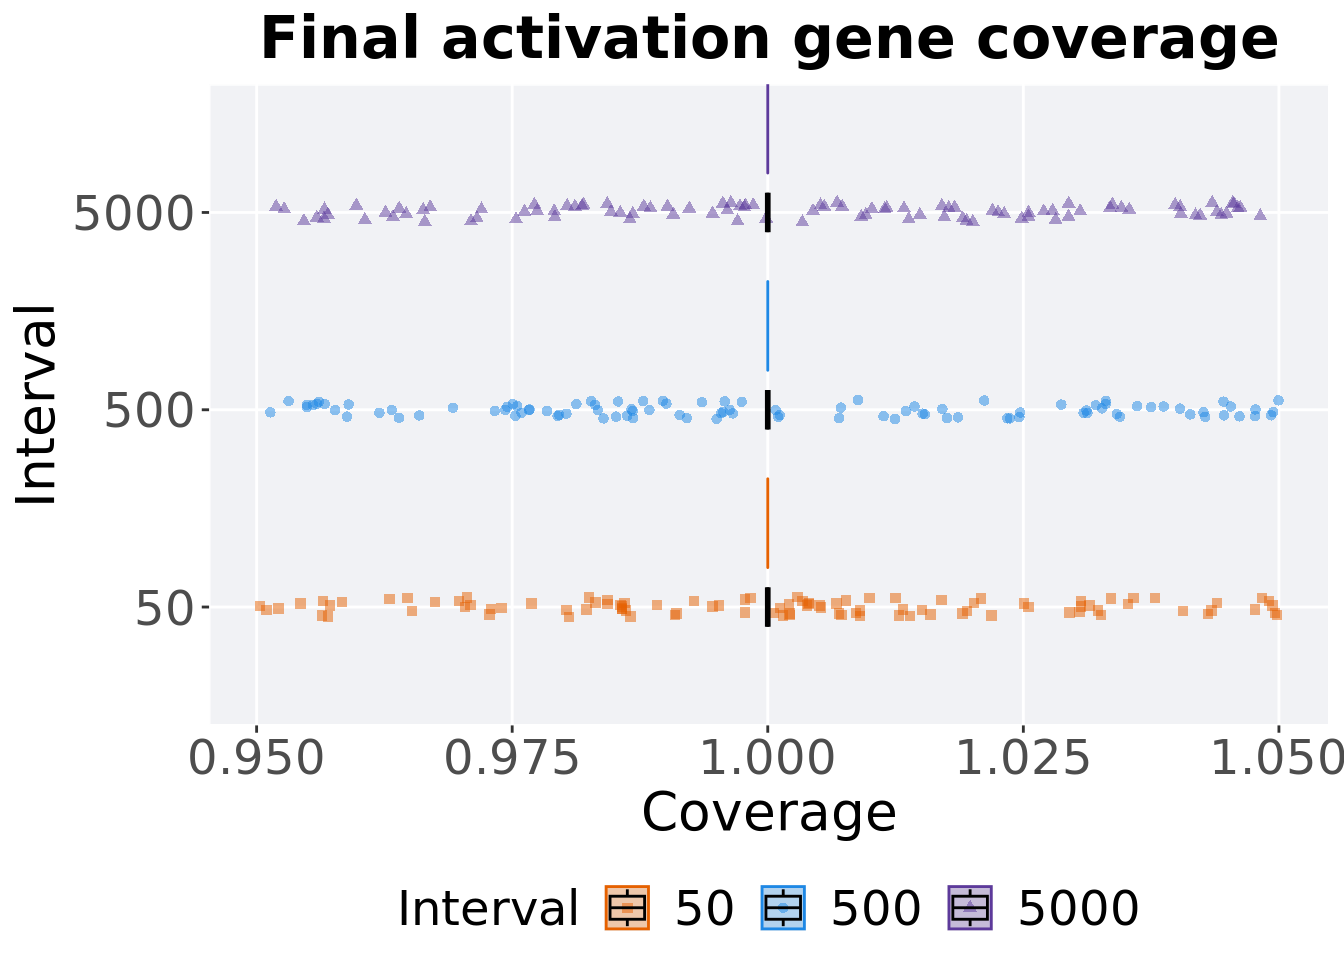
\includegraphics{demo_files/figure-latex/int-con-act-tor-end-1.pdf}

\hypertarget{stats-12}{%
\paragraph{Stats}\label{stats-12}}

Summary statistics for activation gene coverage.

\begin{Shaded}
\begin{Highlighting}[]
\NormalTok{coverage =}\StringTok{ }\KeywordTok{filter}\NormalTok{(df_ot, Diagnostic }\OperatorTok{==}\StringTok{ 'CONTRADICTORY_OBJECTIVES'} \OperatorTok{&}\StringTok{ `}\DataTypeTok{Selection}\CharTok{\textbackslash{}n}\DataTypeTok{Scheme}\StringTok{`} \OperatorTok{==}\StringTok{ 'TOURNAMENT'} \OperatorTok{&}\StringTok{ }\NormalTok{Generations }\OperatorTok{==}\StringTok{ }\DecValTok{50000}\NormalTok{)}
\NormalTok{coverage }\OperatorTok
\StringTok{  }\KeywordTok{group_by}\NormalTok{(Interval) }\OperatorTok
\StringTok{  }\NormalTok{dplyr}\OperatorTok{::}\KeywordTok{summarise}\NormalTok{(}
    \DataTypeTok{count =} \KeywordTok{n}\NormalTok{(),}
    \DataTypeTok{na_cnt =} \KeywordTok{sum}\NormalTok{(}\KeywordTok{is.na}\NormalTok{(pop_act_cov)),}
    \DataTypeTok{min =} \KeywordTok{min}\NormalTok{(pop_act_cov, }\DataTypeTok{na.rm =} \OtherTok{TRUE}\NormalTok{),}
    \DataTypeTok{median =} \KeywordTok{median}\NormalTok{(pop_act_cov, }\DataTypeTok{na.rm =} \OtherTok{TRUE}\NormalTok{),}
    \DataTypeTok{mean =} \KeywordTok{mean}\NormalTok{(pop_act_cov, }\DataTypeTok{na.rm =} \OtherTok{TRUE}\NormalTok{),}
    \DataTypeTok{max =} \KeywordTok{max}\NormalTok{(pop_act_cov, }\DataTypeTok{na.rm =} \OtherTok{TRUE}\NormalTok{),}
    \DataTypeTok{IQR =} \KeywordTok{IQR}\NormalTok{(pop_act_cov, }\DataTypeTok{na.rm =} \OtherTok{TRUE}\NormalTok{)}
\NormalTok{  )}
\end{Highlighting}
\end{Shaded}

\begin{verbatim}
## # A tibble: 3 x 8
##   Interval count na_cnt   min median  mean   max   IQR
##   <fct>    <int>  <int> <int>  <dbl> <dbl> <int> <dbl>
## 1 50         100      0     1      1     1     1     0
## 2 500        100      0     1      1     1     1     0
## 3 5000       100      0     1      1     1     1     0
\end{verbatim}

Kruskal--Wallis test provides evidence of difference among activation gene coverage.

\begin{Shaded}
\begin{Highlighting}[]
\KeywordTok{kruskal.test}\NormalTok{(pop_act_cov }\OperatorTok{~}\StringTok{ }\NormalTok{Interval, }\DataTypeTok{data =}\NormalTok{ coverage)}
\end{Highlighting}
\end{Shaded}

\begin{verbatim}
## 
##  Kruskal-Wallis rank sum test
## 
## data:  pop_act_cov by Interval
## Kruskal-Wallis chi-squared = NaN, df = 2, p-value = NA
\end{verbatim}

Results for post-hoc Wilcoxon rank-sum test with a Bonferroni correction on activation gene coverage.

\begin{Shaded}
\begin{Highlighting}[]
\KeywordTok{pairwise.wilcox.test}\NormalTok{(}\DataTypeTok{x =}\NormalTok{ coverage}\OperatorTok{$}\NormalTok{pop_act_cov, }\DataTypeTok{g =}\NormalTok{ coverage}\OperatorTok{$}\NormalTok{Interval, }\DataTypeTok{p.adjust.method =} \StringTok{"bonferroni"}\NormalTok{,}
                     \DataTypeTok{paired =} \OtherTok{FALSE}\NormalTok{, }\DataTypeTok{conf.int =} \OtherTok{FALSE}\NormalTok{, }\DataTypeTok{alternative =} \StringTok{'g'}\NormalTok{)}
\end{Highlighting}
\end{Shaded}

\begin{verbatim}
## 
##  Pairwise comparisons using Wilcoxon rank sum test with continuity correction 
## 
## data:  coverage$pop_act_cov and coverage$Interval 
## 
##      50 500
## 500  1  -  
## 5000 1  1  
## 
## P value adjustment method: bonferroni
\end{verbatim}

\hypertarget{lexicase-selection-2}{%
\section{Lexicase selection}\label{lexicase-selection-2}}

Here we analyze how the different population structures affect standard lexicase selection on the contradictory objectives diagnostic.

\hypertarget{satisfactory-trait-coverage-2}{%
\subsection{Satisfactory trait coverage}\label{satisfactory-trait-coverage-2}}

Satisfactory trait coverage analysis.

\hypertarget{coverage-over-time-4}{%
\subsubsection{Coverage over time}\label{coverage-over-time-4}}

Satisfactory trait coverage over time.

\begin{Shaded}
\begin{Highlighting}[]
\NormalTok{lines =}\StringTok{ }\KeywordTok{filter}\NormalTok{(df_ot, Diagnostic }\OperatorTok{==}\StringTok{ 'CONTRADICTORY_OBJECTIVES'} \OperatorTok{&}\StringTok{ `}\DataTypeTok{Selection}\CharTok{\textbackslash{}n}\DataTypeTok{Scheme}\StringTok{`} \OperatorTok{==}\StringTok{ 'LEXICASE'}\NormalTok{) }\OperatorTok
\StringTok{  }\KeywordTok{group_by}\NormalTok{(Interval, Generations) }\OperatorTok
\StringTok{  }\NormalTok{dplyr}\OperatorTok{::}\KeywordTok{summarise}\NormalTok{(}
    \DataTypeTok{min =} \KeywordTok{min}\NormalTok{(pop_sat_cov),}
    \DataTypeTok{mean =} \KeywordTok{mean}\NormalTok{(pop_sat_cov),}
    \DataTypeTok{max =} \KeywordTok{max}\NormalTok{(pop_sat_cov)}
\NormalTok{  )}
\end{Highlighting}
\end{Shaded}

\begin{verbatim}
## `summarise()` has grouped output by 'Interval'. You can override using the
## `.groups` argument.
\end{verbatim}

\begin{Shaded}
\begin{Highlighting}[]
\KeywordTok{ggplot}\NormalTok{(lines, }\KeywordTok{aes}\NormalTok{(}\DataTypeTok{x=}\NormalTok{Generations, }\DataTypeTok{y=}\NormalTok{mean, }\DataTypeTok{group =}\NormalTok{ Interval, }\DataTypeTok{fill =}\NormalTok{ Interval, }\DataTypeTok{color =}\NormalTok{ Interval, }\DataTypeTok{shape =}\NormalTok{ Interval)) }\OperatorTok{+}
\StringTok{  }\KeywordTok{geom_ribbon}\NormalTok{(}\KeywordTok{aes}\NormalTok{(}\DataTypeTok{ymin =}\NormalTok{ min, }\DataTypeTok{ymax =}\NormalTok{ max), }\DataTypeTok{alpha =} \FloatTok{0.1}\NormalTok{) }\OperatorTok{+}
\StringTok{  }\KeywordTok{geom_line}\NormalTok{(}\DataTypeTok{size =} \FloatTok{0.5}\NormalTok{) }\OperatorTok{+}
\StringTok{  }\KeywordTok{geom_point}\NormalTok{(}\DataTypeTok{data =} \KeywordTok{filter}\NormalTok{(lines, Generations }\OperatorTok\StringTok{ }\DecValTok{2000} \OperatorTok{==}\StringTok{ }\DecValTok{0}\NormalTok{), }\DataTypeTok{size =} \FloatTok{1.5}\NormalTok{, }\DataTypeTok{stroke =} \FloatTok{2.0}\NormalTok{, }\DataTypeTok{alpha =} \FloatTok{1.0}\NormalTok{) }\OperatorTok{+}
\StringTok{  }\KeywordTok{scale_y_continuous}\NormalTok{(}
    \DataTypeTok{name=}\StringTok{"Coverage"}
\NormalTok{  ) }\OperatorTok{+}
\StringTok{  }\KeywordTok{scale_x_continuous}\NormalTok{(}
    \DataTypeTok{name=}\StringTok{"Generations"}\NormalTok{,}
    \DataTypeTok{limits=}\KeywordTok{c}\NormalTok{(}\DecValTok{0}\NormalTok{, }\DecValTok{50000}\NormalTok{),}
    \DataTypeTok{breaks=}\KeywordTok{c}\NormalTok{(}\DecValTok{0}\NormalTok{, }\DecValTok{10000}\NormalTok{, }\DecValTok{20000}\NormalTok{, }\DecValTok{30000}\NormalTok{, }\DecValTok{40000}\NormalTok{, }\DecValTok{50000}\NormalTok{),}
    \DataTypeTok{labels=}\KeywordTok{c}\NormalTok{(}\StringTok{"0e+4"}\NormalTok{, }\StringTok{"1e+4"}\NormalTok{, }\StringTok{"2e+4"}\NormalTok{, }\StringTok{"3e+4"}\NormalTok{, }\StringTok{"4e+4"}\NormalTok{, }\StringTok{"5e+4"}\NormalTok{)}

\NormalTok{  ) }\OperatorTok{+}
\StringTok{  }\KeywordTok{scale_shape_manual}\NormalTok{(}\DataTypeTok{values=}\NormalTok{SHAPE)}\OperatorTok{+}
\StringTok{  }\KeywordTok{scale_colour_manual}\NormalTok{(}\DataTypeTok{values =}\NormalTok{ cb_palette_mi) }\OperatorTok{+}
\StringTok{  }\KeywordTok{scale_fill_manual}\NormalTok{(}\DataTypeTok{values =}\NormalTok{ cb_palette_mi) }\OperatorTok{+}
\StringTok{  }\KeywordTok{ggtitle}\NormalTok{(}\StringTok{'Satisfactory trait coverage over time'}\NormalTok{)}\OperatorTok{+}
\StringTok{  }\NormalTok{p_theme}
\end{Highlighting}
\end{Shaded}

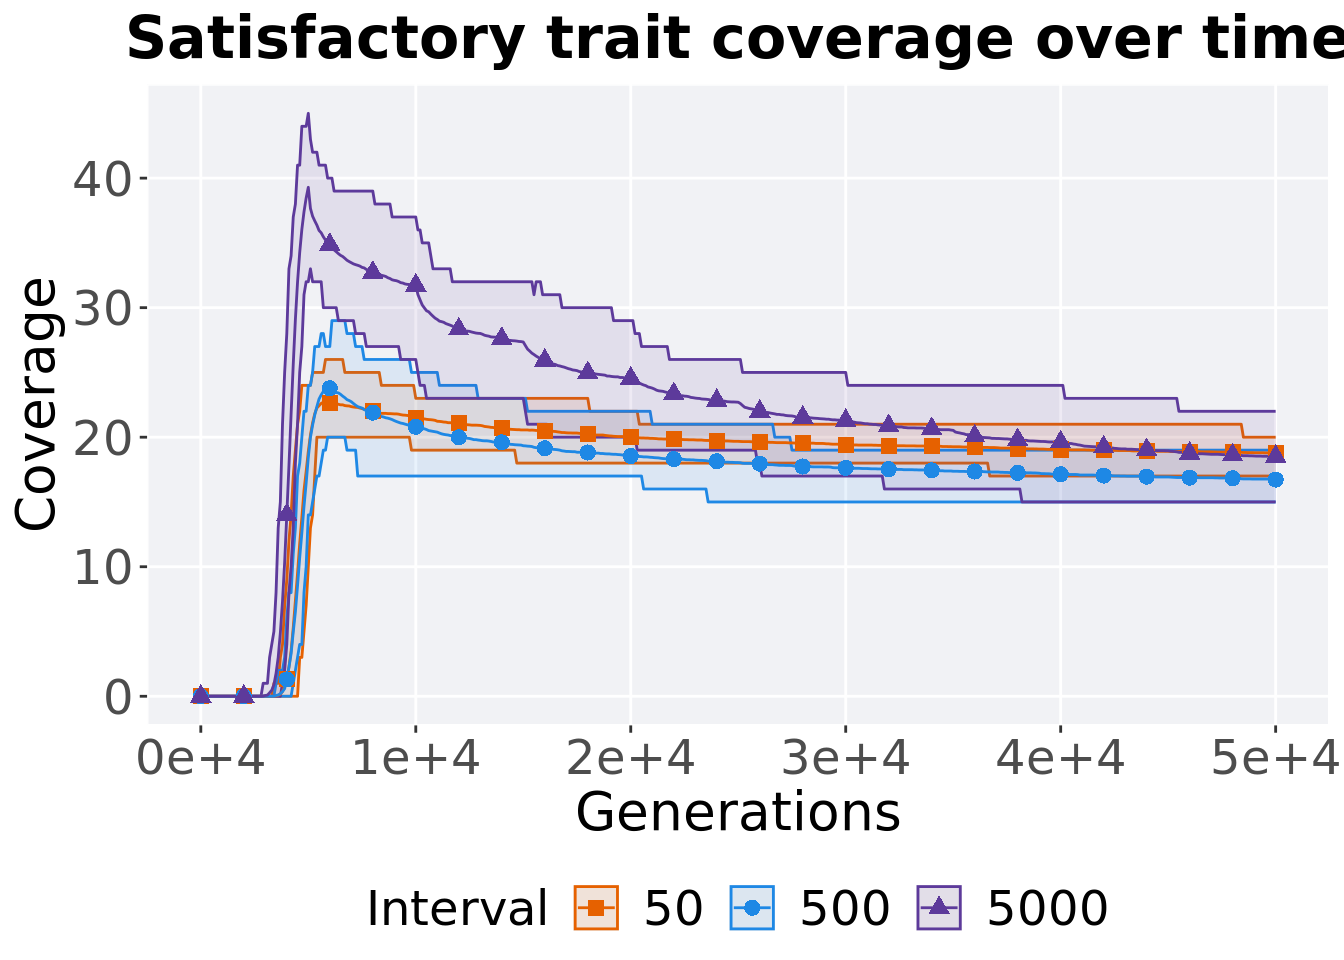
\includegraphics{demo_files/figure-latex/int-con-sat-lex-ot-1.pdf}

\hypertarget{best-coverage-throughout-2}{%
\subsubsection{Best coverage throughout}\label{best-coverage-throughout-2}}

Best satisfactory trait coverage throughout 50,000 generations.

\begin{Shaded}
\begin{Highlighting}[]
\CommentTok{### best satisfactory trait coverage throughout}
\KeywordTok{filter}\NormalTok{(df_best, Diagnostic }\OperatorTok{==}\StringTok{ 'CONTRADICTORY_OBJECTIVES'} \OperatorTok{&}\StringTok{ `}\DataTypeTok{Selection}\CharTok{\textbackslash{}n}\DataTypeTok{Scheme}\StringTok{`} \OperatorTok{==}\StringTok{ 'LEXICASE'} \OperatorTok{&}\StringTok{ }\NormalTok{VAR }\OperatorTok{==}\StringTok{ 'pop_sat_cov'}\NormalTok{) }\OperatorTok
\StringTok{  }\KeywordTok{ggplot}\NormalTok{(., }\KeywordTok{aes}\NormalTok{(}\DataTypeTok{x =}\NormalTok{ Interval, }\DataTypeTok{y =}\NormalTok{ VAL, }\DataTypeTok{color =}\NormalTok{ Interval, }\DataTypeTok{fill =}\NormalTok{ Interval, }\DataTypeTok{shape =}\NormalTok{ Interval)) }\OperatorTok{+}
\StringTok{  }\KeywordTok{geom_flat_violin}\NormalTok{(}\DataTypeTok{position =} \KeywordTok{position_nudge}\NormalTok{(}\DataTypeTok{x =} \FloatTok{.2}\NormalTok{, }\DataTypeTok{y =} \DecValTok{0}\NormalTok{), }\DataTypeTok{scale =} \StringTok{'width'}\NormalTok{, }\DataTypeTok{alpha =} \FloatTok{0.2}\NormalTok{) }\OperatorTok{+}
\StringTok{  }\KeywordTok{geom_point}\NormalTok{(}\DataTypeTok{position =} \KeywordTok{position_jitter}\NormalTok{(}\DataTypeTok{height =} \FloatTok{.05}\NormalTok{, }\DataTypeTok{width =} \FloatTok{.05}\NormalTok{), }\DataTypeTok{size =} \FloatTok{1.5}\NormalTok{, }\DataTypeTok{alpha =} \FloatTok{1.0}\NormalTok{) }\OperatorTok{+}
\StringTok{  }\KeywordTok{geom_boxplot}\NormalTok{(}\DataTypeTok{color =} \StringTok{'black'}\NormalTok{, }\DataTypeTok{width =} \FloatTok{.2}\NormalTok{, }\DataTypeTok{outlier.shape =} \OtherTok{NA}\NormalTok{, }\DataTypeTok{alpha =} \FloatTok{0.0}\NormalTok{) }\OperatorTok{+}
\StringTok{  }\KeywordTok{scale_y_continuous}\NormalTok{(}
    \DataTypeTok{name=}\StringTok{"coverage"}
\NormalTok{  ) }\OperatorTok{+}
\StringTok{  }\KeywordTok{scale_x_discrete}\NormalTok{(}
    \DataTypeTok{name=}\StringTok{"Interval"}
\NormalTok{  )}\OperatorTok{+}
\StringTok{  }\KeywordTok{scale_shape_manual}\NormalTok{(}\DataTypeTok{values=}\NormalTok{SHAPE)}\OperatorTok{+}
\StringTok{  }\KeywordTok{scale_colour_manual}\NormalTok{(}\DataTypeTok{values =}\NormalTok{ cb_palette_mi, ) }\OperatorTok{+}
\StringTok{  }\KeywordTok{scale_fill_manual}\NormalTok{(}\DataTypeTok{values =}\NormalTok{ cb_palette_mi) }\OperatorTok{+}
\StringTok{  }\KeywordTok{ggtitle}\NormalTok{(}\StringTok{'Best satisfactory trait coverage'}\NormalTok{)}\OperatorTok{+}
\StringTok{  }\NormalTok{p_theme }\OperatorTok{+}\StringTok{ }\KeywordTok{coord_flip}\NormalTok{()}
\end{Highlighting}
\end{Shaded}

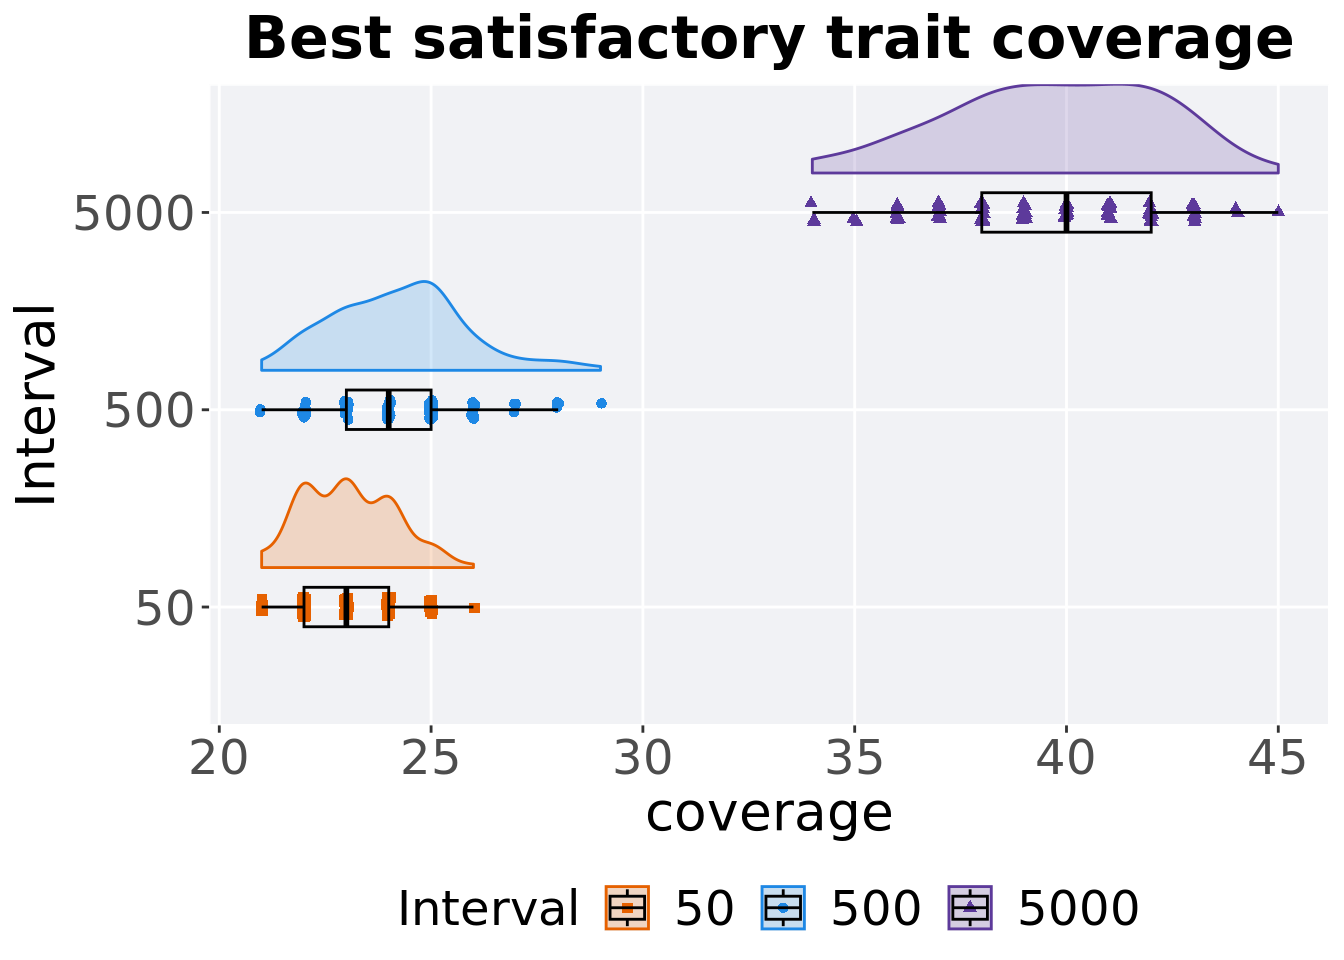
\includegraphics{demo_files/figure-latex/int-con-sat-lex-bst-1.pdf}

\hypertarget{stats-13}{%
\paragraph{Stats}\label{stats-13}}

Summary statistics for the best satisfactory trait coverage.

\begin{Shaded}
\begin{Highlighting}[]
\CommentTok{### best}
\NormalTok{coverage =}\StringTok{ }\KeywordTok{filter}\NormalTok{(df_best, Diagnostic }\OperatorTok{==}\StringTok{ 'CONTRADICTORY_OBJECTIVES'} \OperatorTok{&}\StringTok{ `}\DataTypeTok{Selection}\CharTok{\textbackslash{}n}\DataTypeTok{Scheme}\StringTok{`} \OperatorTok{==}\StringTok{ 'LEXICASE'} \OperatorTok{&}\StringTok{ }\NormalTok{VAR }\OperatorTok{==}\StringTok{ 'pop_sat_cov'}\NormalTok{)}
\NormalTok{coverage}\OperatorTok{$}\NormalTok{Interval =}\StringTok{ }\KeywordTok{factor}\NormalTok{(coverage}\OperatorTok{$}\NormalTok{Interval, }\DataTypeTok{levels=}\KeywordTok{c}\NormalTok{(}\StringTok{'50'}\NormalTok{,}\StringTok{'500'}\NormalTok{,}\StringTok{'5000'}\NormalTok{))}
\NormalTok{coverage }\OperatorTok
\StringTok{  }\KeywordTok{group_by}\NormalTok{(Interval) }\OperatorTok
\StringTok{  }\NormalTok{dplyr}\OperatorTok{::}\KeywordTok{summarise}\NormalTok{(}
    \DataTypeTok{count =} \KeywordTok{n}\NormalTok{(),}
    \DataTypeTok{na_cnt =} \KeywordTok{sum}\NormalTok{(}\KeywordTok{is.na}\NormalTok{(VAL)),}
    \DataTypeTok{min =} \KeywordTok{min}\NormalTok{(VAL, }\DataTypeTok{na.rm =} \OtherTok{TRUE}\NormalTok{),}
    \DataTypeTok{median =} \KeywordTok{median}\NormalTok{(VAL, }\DataTypeTok{na.rm =} \OtherTok{TRUE}\NormalTok{),}
    \DataTypeTok{mean =} \KeywordTok{mean}\NormalTok{(VAL, }\DataTypeTok{na.rm =} \OtherTok{TRUE}\NormalTok{),}
    \DataTypeTok{max =} \KeywordTok{max}\NormalTok{(VAL, }\DataTypeTok{na.rm =} \OtherTok{TRUE}\NormalTok{),}
    \DataTypeTok{IQR =} \KeywordTok{IQR}\NormalTok{(VAL, }\DataTypeTok{na.rm =} \OtherTok{TRUE}\NormalTok{)}
\NormalTok{  )}
\end{Highlighting}
\end{Shaded}

\begin{verbatim}
## # A tibble: 3 x 8
##   Interval count na_cnt   min median  mean   max   IQR
##   <fct>    <int>  <int> <dbl>  <dbl> <dbl> <dbl> <dbl>
## 1 50         100      0    21     23  23.0    26     2
## 2 500        100      0    21     24  24.2    29     2
## 3 5000       100      0    34     40  39.7    45     4
\end{verbatim}

Kruskal--Wallis test provides evidence of difference among satisfactory trait coverage.

\begin{Shaded}
\begin{Highlighting}[]
\KeywordTok{kruskal.test}\NormalTok{(VAL }\OperatorTok{~}\StringTok{ }\NormalTok{Interval, }\DataTypeTok{data =}\NormalTok{ coverage)}
\end{Highlighting}
\end{Shaded}

\begin{verbatim}
## 
##  Kruskal-Wallis rank sum test
## 
## data:  VAL by Interval
## Kruskal-Wallis chi-squared = 216.13, df = 2, p-value < 2.2e-16
\end{verbatim}

Results for post-hoc Wilcoxon rank-sum test with a Bonferroni correction on satisfactory trait coverage.

\begin{Shaded}
\begin{Highlighting}[]
\KeywordTok{pairwise.wilcox.test}\NormalTok{(}\DataTypeTok{x =}\NormalTok{ coverage}\OperatorTok{$}\NormalTok{VAL, }\DataTypeTok{g =}\NormalTok{ coverage}\OperatorTok{$}\NormalTok{Interval, }\DataTypeTok{p.adjust.method =} \StringTok{"bonferroni"}\NormalTok{,}
                     \DataTypeTok{paired =} \OtherTok{FALSE}\NormalTok{, }\DataTypeTok{conf.int =} \OtherTok{FALSE}\NormalTok{, }\DataTypeTok{alternative =} \StringTok{'g'}\NormalTok{)}
\end{Highlighting}
\end{Shaded}

\begin{verbatim}
## 
##  Pairwise comparisons using Wilcoxon rank sum test with continuity correction 
## 
## data:  coverage$VAL and coverage$Interval 
## 
##      50      500    
## 500  1.8e-08 -      
## 5000 < 2e-16 < 2e-16
## 
## P value adjustment method: bonferroni
\end{verbatim}

\hypertarget{end-of-50000-generations-4}{%
\subsubsection{End of 50,000 generations}\label{end-of-50000-generations-4}}

Satisfactory trait coverage in the population at the end of 50,000 generations.

\begin{Shaded}
\begin{Highlighting}[]
\CommentTok{### end of run}
\KeywordTok{filter}\NormalTok{(df_ot, Diagnostic }\OperatorTok{==}\StringTok{ 'CONTRADICTORY_OBJECTIVES'} \OperatorTok{&}\StringTok{ `}\DataTypeTok{Selection}\CharTok{\textbackslash{}n}\DataTypeTok{Scheme}\StringTok{`} \OperatorTok{==}\StringTok{ 'LEXICASE'} \OperatorTok{&}\StringTok{ }\NormalTok{Generations }\OperatorTok{==}\StringTok{ }\DecValTok{50000}\NormalTok{) }\OperatorTok
\StringTok{  }\KeywordTok{ggplot}\NormalTok{(., }\KeywordTok{aes}\NormalTok{(}\DataTypeTok{x =}\NormalTok{ Interval, }\DataTypeTok{y =}\NormalTok{ pop_sat_cov, }\DataTypeTok{color =}\NormalTok{ Interval, }\DataTypeTok{fill =}\NormalTok{ Interval, }\DataTypeTok{shape =}\NormalTok{ Interval)) }\OperatorTok{+}
\StringTok{  }\KeywordTok{geom_flat_violin}\NormalTok{(}\DataTypeTok{position =} \KeywordTok{position_nudge}\NormalTok{(}\DataTypeTok{x =} \FloatTok{.2}\NormalTok{, }\DataTypeTok{y =} \DecValTok{0}\NormalTok{), }\DataTypeTok{scale =} \StringTok{'width'}\NormalTok{, }\DataTypeTok{alpha =} \FloatTok{0.3}\NormalTok{) }\OperatorTok{+}
\StringTok{  }\KeywordTok{geom_point}\NormalTok{(}\DataTypeTok{position =} \KeywordTok{position_jitter}\NormalTok{(}\DataTypeTok{height =} \FloatTok{.05}\NormalTok{, }\DataTypeTok{width =} \FloatTok{.05}\NormalTok{), }\DataTypeTok{size =} \FloatTok{1.5}\NormalTok{, }\DataTypeTok{alpha =} \FloatTok{0.5}\NormalTok{) }\OperatorTok{+}
\StringTok{  }\KeywordTok{geom_boxplot}\NormalTok{(}\DataTypeTok{color =} \StringTok{'black'}\NormalTok{, }\DataTypeTok{width =} \FloatTok{.2}\NormalTok{, }\DataTypeTok{outlier.shape =} \OtherTok{NA}\NormalTok{, }\DataTypeTok{alpha =} \FloatTok{0.0}\NormalTok{) }\OperatorTok{+}
\StringTok{  }\KeywordTok{scale_shape_manual}\NormalTok{(}\DataTypeTok{values=}\NormalTok{SHAPE)}\OperatorTok{+}
\StringTok{  }\KeywordTok{scale_y_continuous}\NormalTok{(}
    \DataTypeTok{name=}\StringTok{"Coverage"}
\NormalTok{  ) }\OperatorTok{+}
\StringTok{  }\KeywordTok{scale_x_discrete}\NormalTok{(}
    \DataTypeTok{name=}\StringTok{"Interval"}
\NormalTok{  ) }\OperatorTok{+}
\StringTok{  }\KeywordTok{scale_colour_manual}\NormalTok{(}\DataTypeTok{values =}\NormalTok{ cb_palette_mi) }\OperatorTok{+}
\StringTok{  }\KeywordTok{scale_fill_manual}\NormalTok{(}\DataTypeTok{values =}\NormalTok{ cb_palette_mi) }\OperatorTok{+}
\StringTok{  }\KeywordTok{ggtitle}\NormalTok{(}\StringTok{'Final satisfactory trait coverage'}\NormalTok{)}\OperatorTok{+}
\StringTok{  }\NormalTok{p_theme }\OperatorTok{+}\StringTok{ }\KeywordTok{coord_flip}\NormalTok{()}
\end{Highlighting}
\end{Shaded}

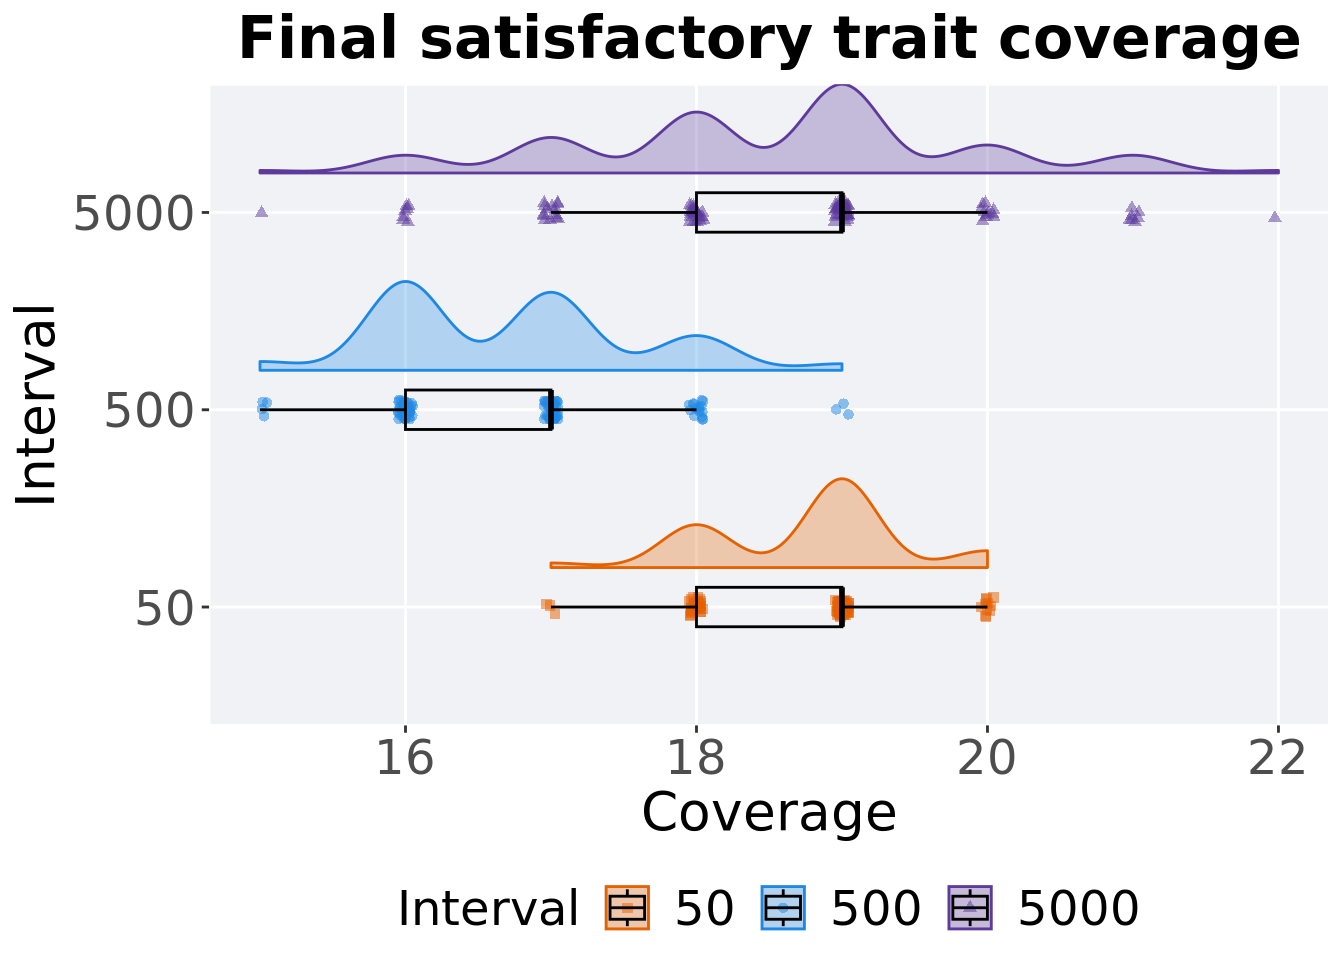
\includegraphics{demo_files/figure-latex/int-con-sat-lex-end-1.pdf}

\hypertarget{stats-14}{%
\paragraph{Stats}\label{stats-14}}

Summary statistics for satisfactory trait coverage in the population at the end of 50,000 generations.

\begin{Shaded}
\begin{Highlighting}[]
\CommentTok{### end of run}
\NormalTok{coverage =}\StringTok{ }\KeywordTok{filter}\NormalTok{(df_ot, Diagnostic }\OperatorTok{==}\StringTok{ 'CONTRADICTORY_OBJECTIVES'} \OperatorTok{&}\StringTok{ `}\DataTypeTok{Selection}\CharTok{\textbackslash{}n}\DataTypeTok{Scheme}\StringTok{`} \OperatorTok{==}\StringTok{ 'LEXICASE'} \OperatorTok{&}\StringTok{ }\NormalTok{Generations }\OperatorTok{==}\StringTok{ }\DecValTok{50000}\NormalTok{)}
\NormalTok{coverage}\OperatorTok{$}\NormalTok{Interval =}\StringTok{ }\KeywordTok{factor}\NormalTok{(coverage}\OperatorTok{$}\NormalTok{Interval, }\DataTypeTok{levels=}\KeywordTok{c}\NormalTok{(}\StringTok{'500'}\NormalTok{,}\StringTok{'50'}\NormalTok{,}\StringTok{'5000'}\NormalTok{))}
\NormalTok{coverage }\OperatorTok
\StringTok{  }\KeywordTok{group_by}\NormalTok{(Interval) }\OperatorTok
\StringTok{  }\NormalTok{dplyr}\OperatorTok{::}\KeywordTok{summarise}\NormalTok{(}
    \DataTypeTok{count =} \KeywordTok{n}\NormalTok{(),}
    \DataTypeTok{na_cnt =} \KeywordTok{sum}\NormalTok{(}\KeywordTok{is.na}\NormalTok{(pop_sat_cov)),}
    \DataTypeTok{min =} \KeywordTok{min}\NormalTok{(pop_sat_cov, }\DataTypeTok{na.rm =} \OtherTok{TRUE}\NormalTok{),}
    \DataTypeTok{median =} \KeywordTok{median}\NormalTok{(pop_sat_cov, }\DataTypeTok{na.rm =} \OtherTok{TRUE}\NormalTok{),}
    \DataTypeTok{mean =} \KeywordTok{mean}\NormalTok{(pop_sat_cov, }\DataTypeTok{na.rm =} \OtherTok{TRUE}\NormalTok{),}
    \DataTypeTok{max =} \KeywordTok{max}\NormalTok{(pop_sat_cov, }\DataTypeTok{na.rm =} \OtherTok{TRUE}\NormalTok{),}
    \DataTypeTok{IQR =} \KeywordTok{IQR}\NormalTok{(pop_sat_cov, }\DataTypeTok{na.rm =} \OtherTok{TRUE}\NormalTok{)}
\NormalTok{  )}
\end{Highlighting}
\end{Shaded}

\begin{verbatim}
## # A tibble: 3 x 8
##   Interval count na_cnt   min median  mean   max   IQR
##   <fct>    <int>  <int> <int>  <dbl> <dbl> <int> <dbl>
## 1 500        100      0    15     17  16.7    19     1
## 2 50         100      0    17     19  18.8    20     1
## 3 5000       100      0    15     19  18.5    22     1
\end{verbatim}

Kruskal--Wallis test provides evidence of difference among satisfactory trait coverage in the population at the end of 50,000 generations.

\begin{Shaded}
\begin{Highlighting}[]
\KeywordTok{kruskal.test}\NormalTok{(pop_sat_cov }\OperatorTok{~}\StringTok{ }\NormalTok{Interval, }\DataTypeTok{data =}\NormalTok{ coverage)}
\end{Highlighting}
\end{Shaded}

\begin{verbatim}
## 
##  Kruskal-Wallis rank sum test
## 
## data:  pop_sat_cov by Interval
## Kruskal-Wallis chi-squared = 139.49, df = 2, p-value < 2.2e-16
\end{verbatim}

Results for post-hoc Wilcoxon rank-sum test with a Bonferroni correction on satisfactory trait coverage in the population at the end of 50,000 generations.

\begin{Shaded}
\begin{Highlighting}[]
\KeywordTok{pairwise.wilcox.test}\NormalTok{(}\DataTypeTok{x =}\NormalTok{ coverage}\OperatorTok{$}\NormalTok{pop_sat_cov, }\DataTypeTok{g =}\NormalTok{ coverage}\OperatorTok{$}\NormalTok{Interval, }\DataTypeTok{p.adjust.method =} \StringTok{"bonferroni"}\NormalTok{,}
                     \DataTypeTok{paired =} \OtherTok{FALSE}\NormalTok{, }\DataTypeTok{conf.int =} \OtherTok{FALSE}\NormalTok{, }\DataTypeTok{alternative =} \StringTok{'g'}\NormalTok{)}
\end{Highlighting}
\end{Shaded}

\begin{verbatim}
## 
##  Pairwise comparisons using Wilcoxon rank sum test with continuity correction 
## 
## data:  coverage$pop_sat_cov and coverage$Interval 
## 
##      500    50
## 50   <2e-16 - 
## 5000 <2e-16 1 
## 
## P value adjustment method: bonferroni
\end{verbatim}

\hypertarget{activation-gene-coverage-2}{%
\subsection{Activation gene coverage}\label{activation-gene-coverage-2}}

Activation gene coverage analysis.

\hypertarget{coverage-over-time-5}{%
\subsubsection{Coverage over time}\label{coverage-over-time-5}}

Activation gene coverage over time.

\begin{Shaded}
\begin{Highlighting}[]
\CommentTok{# data for lines and shading on plots}
\NormalTok{lines =}\StringTok{ }\KeywordTok{filter}\NormalTok{(df_ot, Diagnostic }\OperatorTok{==}\StringTok{ 'CONTRADICTORY_OBJECTIVES'} \OperatorTok{&}\StringTok{ `}\DataTypeTok{Selection}\CharTok{\textbackslash{}n}\DataTypeTok{Scheme}\StringTok{`} \OperatorTok{==}\StringTok{ 'LEXICASE'}\NormalTok{) }\OperatorTok
\StringTok{  }\KeywordTok{group_by}\NormalTok{(Interval, Generations) }\OperatorTok
\StringTok{  }\NormalTok{dplyr}\OperatorTok{::}\KeywordTok{summarise}\NormalTok{(}
    \DataTypeTok{min =} \KeywordTok{min}\NormalTok{(pop_act_cov),}
    \DataTypeTok{mean =} \KeywordTok{mean}\NormalTok{(pop_act_cov),}
    \DataTypeTok{max =} \KeywordTok{max}\NormalTok{(pop_act_cov)}
\NormalTok{  )}
\end{Highlighting}
\end{Shaded}

\begin{verbatim}
## `summarise()` has grouped output by 'Interval'. You can override using the
## `.groups` argument.
\end{verbatim}

\begin{Shaded}
\begin{Highlighting}[]
\KeywordTok{ggplot}\NormalTok{(lines, }\KeywordTok{aes}\NormalTok{(}\DataTypeTok{x=}\NormalTok{Generations, }\DataTypeTok{y=}\NormalTok{mean, }\DataTypeTok{group =}\NormalTok{ Interval, }\DataTypeTok{fill =}\NormalTok{ Interval, }\DataTypeTok{color =}\NormalTok{ Interval, }\DataTypeTok{shape =}\NormalTok{ Interval)) }\OperatorTok{+}
\StringTok{  }\KeywordTok{geom_ribbon}\NormalTok{(}\KeywordTok{aes}\NormalTok{(}\DataTypeTok{ymin =}\NormalTok{ min, }\DataTypeTok{ymax =}\NormalTok{ max), }\DataTypeTok{alpha =} \FloatTok{0.1}\NormalTok{) }\OperatorTok{+}
\StringTok{  }\KeywordTok{geom_line}\NormalTok{(}\DataTypeTok{size =} \FloatTok{0.5}\NormalTok{) }\OperatorTok{+}
\StringTok{  }\KeywordTok{geom_point}\NormalTok{(}\DataTypeTok{data =} \KeywordTok{filter}\NormalTok{(lines, Generations }\OperatorTok\StringTok{ }\DecValTok{2000} \OperatorTok{==}\StringTok{ }\DecValTok{0}\NormalTok{), }\DataTypeTok{size =} \FloatTok{1.5}\NormalTok{, }\DataTypeTok{stroke =} \FloatTok{2.0}\NormalTok{, }\DataTypeTok{alpha =} \FloatTok{1.0}\NormalTok{) }\OperatorTok{+}
\StringTok{  }\KeywordTok{scale_y_continuous}\NormalTok{(}
    \DataTypeTok{name=}\StringTok{"Coverage"}
\NormalTok{  ) }\OperatorTok{+}
\StringTok{  }\KeywordTok{scale_x_continuous}\NormalTok{(}
    \DataTypeTok{name=}\StringTok{"Generations"}\NormalTok{,}
    \DataTypeTok{limits=}\KeywordTok{c}\NormalTok{(}\DecValTok{0}\NormalTok{, }\DecValTok{50000}\NormalTok{),}
    \DataTypeTok{breaks=}\KeywordTok{c}\NormalTok{(}\DecValTok{0}\NormalTok{, }\DecValTok{10000}\NormalTok{, }\DecValTok{20000}\NormalTok{, }\DecValTok{30000}\NormalTok{, }\DecValTok{40000}\NormalTok{, }\DecValTok{50000}\NormalTok{),}
    \DataTypeTok{labels=}\KeywordTok{c}\NormalTok{(}\StringTok{"0e+4"}\NormalTok{, }\StringTok{"1e+4"}\NormalTok{, }\StringTok{"2e+4"}\NormalTok{, }\StringTok{"3e+4"}\NormalTok{, }\StringTok{"4e+4"}\NormalTok{, }\StringTok{"5e+4"}\NormalTok{)}

\NormalTok{  ) }\OperatorTok{+}
\StringTok{  }\KeywordTok{scale_shape_manual}\NormalTok{(}\DataTypeTok{values=}\NormalTok{SHAPE)}\OperatorTok{+}
\StringTok{  }\KeywordTok{scale_colour_manual}\NormalTok{(}\DataTypeTok{values =}\NormalTok{ cb_palette_mi) }\OperatorTok{+}
\StringTok{  }\KeywordTok{scale_fill_manual}\NormalTok{(}\DataTypeTok{values =}\NormalTok{ cb_palette_mi) }\OperatorTok{+}
\StringTok{  }\KeywordTok{ggtitle}\NormalTok{(}\StringTok{'Activation gene coverage over time'}\NormalTok{)}\OperatorTok{+}
\StringTok{  }\NormalTok{p_theme}
\end{Highlighting}
\end{Shaded}

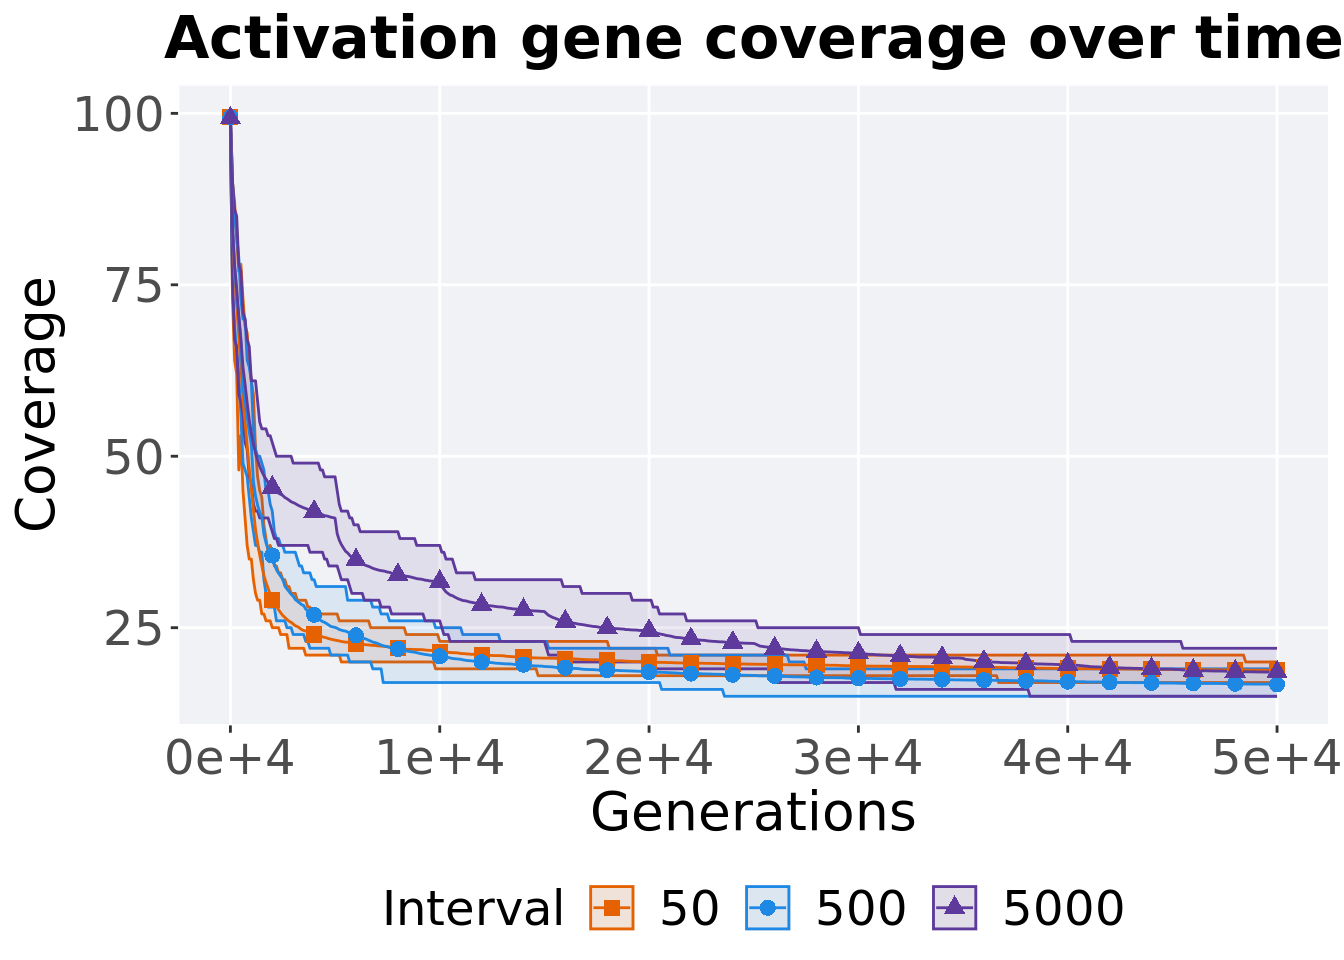
\includegraphics{demo_files/figure-latex/int-con-act-lex-ot-1.pdf}

\hypertarget{end-of-50000-generations-5}{%
\subsubsection{End of 50,000 generations}\label{end-of-50000-generations-5}}

Activation gene coverage in the population at the end of 50,000 generations.

\begin{Shaded}
\begin{Highlighting}[]
\CommentTok{### end of run}
\KeywordTok{filter}\NormalTok{(df_ot, Diagnostic }\OperatorTok{==}\StringTok{ 'CONTRADICTORY_OBJECTIVES'} \OperatorTok{&}\StringTok{ `}\DataTypeTok{Selection}\CharTok{\textbackslash{}n}\DataTypeTok{Scheme}\StringTok{`} \OperatorTok{==}\StringTok{ 'LEXICASE'} \OperatorTok{&}\StringTok{ }\NormalTok{Generations }\OperatorTok{==}\StringTok{ }\DecValTok{50000}\NormalTok{) }\OperatorTok
\StringTok{  }\KeywordTok{ggplot}\NormalTok{(., }\KeywordTok{aes}\NormalTok{(}\DataTypeTok{x =}\NormalTok{ Interval, }\DataTypeTok{y =}\NormalTok{ pop_act_cov, }\DataTypeTok{color =}\NormalTok{ Interval, }\DataTypeTok{fill =}\NormalTok{ Interval, }\DataTypeTok{shape =}\NormalTok{ Interval)) }\OperatorTok{+}
\StringTok{  }\KeywordTok{geom_flat_violin}\NormalTok{(}\DataTypeTok{position =} \KeywordTok{position_nudge}\NormalTok{(}\DataTypeTok{x =} \FloatTok{.2}\NormalTok{, }\DataTypeTok{y =} \DecValTok{0}\NormalTok{), }\DataTypeTok{scale =} \StringTok{'width'}\NormalTok{, }\DataTypeTok{alpha =} \FloatTok{0.3}\NormalTok{) }\OperatorTok{+}
\StringTok{  }\KeywordTok{geom_point}\NormalTok{(}\DataTypeTok{position =} \KeywordTok{position_jitter}\NormalTok{(}\DataTypeTok{height =} \FloatTok{.05}\NormalTok{, }\DataTypeTok{width =} \FloatTok{.05}\NormalTok{), }\DataTypeTok{size =} \FloatTok{1.5}\NormalTok{, }\DataTypeTok{alpha =} \FloatTok{0.5}\NormalTok{) }\OperatorTok{+}
\StringTok{  }\KeywordTok{geom_boxplot}\NormalTok{(}\DataTypeTok{color =} \StringTok{'black'}\NormalTok{, }\DataTypeTok{width =} \FloatTok{.2}\NormalTok{, }\DataTypeTok{outlier.shape =} \OtherTok{NA}\NormalTok{, }\DataTypeTok{alpha =} \FloatTok{0.0}\NormalTok{) }\OperatorTok{+}
\StringTok{  }\KeywordTok{scale_shape_manual}\NormalTok{(}\DataTypeTok{values=}\NormalTok{SHAPE)}\OperatorTok{+}
\StringTok{  }\KeywordTok{scale_y_continuous}\NormalTok{(}
    \DataTypeTok{name=}\StringTok{"Coverage"}
\NormalTok{  ) }\OperatorTok{+}
\StringTok{  }\KeywordTok{scale_x_discrete}\NormalTok{(}
    \DataTypeTok{name=}\StringTok{"Interval"}
\NormalTok{  ) }\OperatorTok{+}
\StringTok{  }\KeywordTok{scale_colour_manual}\NormalTok{(}\DataTypeTok{values =}\NormalTok{ cb_palette_mi) }\OperatorTok{+}
\StringTok{  }\KeywordTok{scale_fill_manual}\NormalTok{(}\DataTypeTok{values =}\NormalTok{ cb_palette_mi) }\OperatorTok{+}
\StringTok{  }\KeywordTok{ggtitle}\NormalTok{(}\StringTok{'Final activation gene coverage'}\NormalTok{)}\OperatorTok{+}
\StringTok{  }\NormalTok{p_theme }\OperatorTok{+}\StringTok{ }\KeywordTok{coord_flip}\NormalTok{()}
\end{Highlighting}
\end{Shaded}

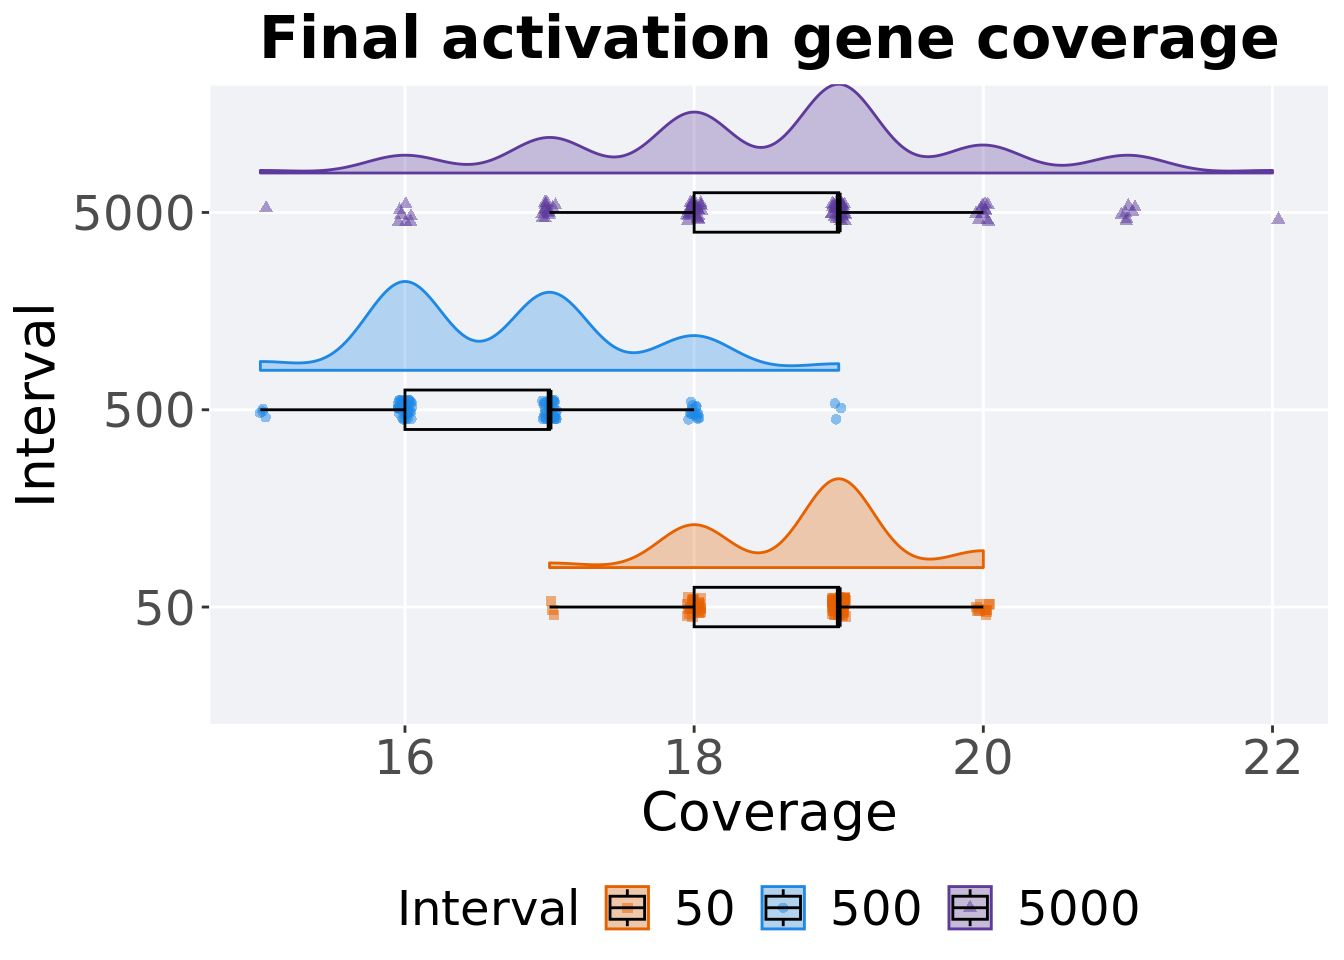
\includegraphics{demo_files/figure-latex/int-con-act-lex-end-1.pdf}

\hypertarget{stats-15}{%
\paragraph{Stats}\label{stats-15}}

Summary statistics for activation gene coverage.

\begin{Shaded}
\begin{Highlighting}[]
\NormalTok{coverage =}\StringTok{ }\KeywordTok{filter}\NormalTok{(df_ot, Diagnostic }\OperatorTok{==}\StringTok{ 'CONTRADICTORY_OBJECTIVES'} \OperatorTok{&}\StringTok{ `}\DataTypeTok{Selection}\CharTok{\textbackslash{}n}\DataTypeTok{Scheme}\StringTok{`} \OperatorTok{==}\StringTok{ 'LEXICASE'} \OperatorTok{&}\StringTok{ }\NormalTok{Generations }\OperatorTok{==}\StringTok{ }\DecValTok{50000}\NormalTok{)}
\NormalTok{coverage}\OperatorTok{$}\NormalTok{Interval =}\StringTok{ }\KeywordTok{factor}\NormalTok{(coverage}\OperatorTok{$}\NormalTok{Interval, }\DataTypeTok{levels=}\KeywordTok{c}\NormalTok{(}\StringTok{'500'}\NormalTok{,}\StringTok{'50'}\NormalTok{,}\StringTok{'5000'}\NormalTok{))}
\NormalTok{coverage }\OperatorTok
\StringTok{  }\KeywordTok{group_by}\NormalTok{(Interval) }\OperatorTok
\StringTok{  }\NormalTok{dplyr}\OperatorTok{::}\KeywordTok{summarise}\NormalTok{(}
    \DataTypeTok{count =} \KeywordTok{n}\NormalTok{(),}
    \DataTypeTok{na_cnt =} \KeywordTok{sum}\NormalTok{(}\KeywordTok{is.na}\NormalTok{(pop_act_cov)),}
    \DataTypeTok{min =} \KeywordTok{min}\NormalTok{(pop_act_cov, }\DataTypeTok{na.rm =} \OtherTok{TRUE}\NormalTok{),}
    \DataTypeTok{median =} \KeywordTok{median}\NormalTok{(pop_act_cov, }\DataTypeTok{na.rm =} \OtherTok{TRUE}\NormalTok{),}
    \DataTypeTok{mean =} \KeywordTok{mean}\NormalTok{(pop_act_cov, }\DataTypeTok{na.rm =} \OtherTok{TRUE}\NormalTok{),}
    \DataTypeTok{max =} \KeywordTok{max}\NormalTok{(pop_act_cov, }\DataTypeTok{na.rm =} \OtherTok{TRUE}\NormalTok{),}
    \DataTypeTok{IQR =} \KeywordTok{IQR}\NormalTok{(pop_act_cov, }\DataTypeTok{na.rm =} \OtherTok{TRUE}\NormalTok{)}
\NormalTok{  )}
\end{Highlighting}
\end{Shaded}

\begin{verbatim}
## # A tibble: 3 x 8
##   Interval count na_cnt   min median  mean   max   IQR
##   <fct>    <int>  <int> <int>  <dbl> <dbl> <int> <dbl>
## 1 500        100      0    15     17  16.7    19     1
## 2 50         100      0    17     19  18.8    20     1
## 3 5000       100      0    15     19  18.5    22     1
\end{verbatim}

Kruskal--Wallis test provides evidence of difference among activation gene coverage.

\begin{Shaded}
\begin{Highlighting}[]
\KeywordTok{kruskal.test}\NormalTok{(pop_act_cov }\OperatorTok{~}\StringTok{ }\NormalTok{Interval, }\DataTypeTok{data =}\NormalTok{ coverage)}
\end{Highlighting}
\end{Shaded}

\begin{verbatim}
## 
##  Kruskal-Wallis rank sum test
## 
## data:  pop_act_cov by Interval
## Kruskal-Wallis chi-squared = 139.49, df = 2, p-value < 2.2e-16
\end{verbatim}

Results for post-hoc Wilcoxon rank-sum test with a Bonferroni correction on activation gene coverage.

\begin{Shaded}
\begin{Highlighting}[]
\KeywordTok{pairwise.wilcox.test}\NormalTok{(}\DataTypeTok{x =}\NormalTok{ coverage}\OperatorTok{$}\NormalTok{pop_act_cov, }\DataTypeTok{g =}\NormalTok{ coverage}\OperatorTok{$}\NormalTok{Interval, }\DataTypeTok{p.adjust.method =} \StringTok{"bonferroni"}\NormalTok{,}
                     \DataTypeTok{paired =} \OtherTok{FALSE}\NormalTok{, }\DataTypeTok{conf.int =} \OtherTok{FALSE}\NormalTok{, }\DataTypeTok{alternative =} \StringTok{'g'}\NormalTok{)}
\end{Highlighting}
\end{Shaded}

\begin{verbatim}
## 
##  Pairwise comparisons using Wilcoxon rank sum test with continuity correction 
## 
## data:  coverage$pop_act_cov and coverage$Interval 
## 
##      500    50
## 50   <2e-16 - 
## 5000 <2e-16 1 
## 
## P value adjustment method: bonferroni
\end{verbatim}

\hypertarget{mi500-multi-path-exploration-results}{%
\chapter{MI500: Multi-path exploration results}\label{mi500-multi-path-exploration-results}}

Here we present the results for the \textbf{best performances} and \textbf{activation gene coverage} generated by each selection scheme replicate on the multi-path exploration diagnostic.
Best performance found refers to the largest average trait score found in a given population.
Note that activation gene coverage values are gathered at the population-level.
Activation gene coverage refers to the count of unique activation genes in a given population; this gives us a range of integers between 0 and 100.

\hypertarget{analysis-dependencies-3}{%
\section{Analysis dependencies}\label{analysis-dependencies-3}}

\begin{Shaded}
\begin{Highlighting}[]
\KeywordTok{library}\NormalTok{(ggplot2)}
\KeywordTok{library}\NormalTok{(cowplot)}
\KeywordTok{library}\NormalTok{(dplyr)}
\KeywordTok{library}\NormalTok{(PupillometryR)}
\end{Highlighting}
\end{Shaded}

\hypertarget{data-3}{%
\section{Data}\label{data-3}}

\begin{Shaded}
\begin{Highlighting}[]
\NormalTok{base   =}\StringTok{ }\KeywordTok{filter}\NormalTok{(base_over_time,   Diagnostic }\OperatorTok{==}\StringTok{ 'MULTIPATH_EXPLORATION'} \OperatorTok{&}\StringTok{ }\NormalTok{Structure }\OperatorTok{==}\StringTok{ 'IS'}\NormalTok{)}
\NormalTok{mi50   =}\StringTok{ }\KeywordTok{filter}\NormalTok{(mi50_over_time,   Diagnostic }\OperatorTok{==}\StringTok{ 'MULTIPATH_EXPLORATION'} \OperatorTok{&}\StringTok{ }\NormalTok{Structure }\OperatorTok{==}\StringTok{ 'IS'}\NormalTok{)}
\NormalTok{mi5000 =}\StringTok{ }\KeywordTok{filter}\NormalTok{(mi5000_over_time, Diagnostic }\OperatorTok{==}\StringTok{ 'MULTIPATH_EXPLORATION'} \OperatorTok{&}\StringTok{ }\NormalTok{Structure }\OperatorTok{==}\StringTok{ 'IS'}\NormalTok{)}

\NormalTok{base}\OperatorTok{$}\NormalTok{Interval =}\StringTok{ '500'}
\NormalTok{mi50}\OperatorTok{$}\NormalTok{Interval =}\StringTok{ '50'}
\NormalTok{mi5000}\OperatorTok{$}\NormalTok{Interval =}\StringTok{ '5000'}

\NormalTok{df_ot =}\StringTok{ }\KeywordTok{rbind}\NormalTok{(base, mi50, mi5000)}
\NormalTok{df_ot}\OperatorTok{$}\NormalTok{Interval =}\StringTok{ }\KeywordTok{factor}\NormalTok{(df_ot}\OperatorTok{$}\NormalTok{Interval, }\DataTypeTok{levels=}\KeywordTok{c}\NormalTok{(}\StringTok{'50'}\NormalTok{,}\StringTok{'500'}\NormalTok{,}\StringTok{'5000'}\NormalTok{))}

\NormalTok{base =}\StringTok{ }\KeywordTok{filter}\NormalTok{(base_best,     Diagnostic }\OperatorTok{==}\StringTok{ 'MULTIPATH_EXPLORATION'} \OperatorTok{&}\StringTok{ }\NormalTok{Structure }\OperatorTok{==}\StringTok{ 'IS'}\NormalTok{)}
\NormalTok{mi50 =}\StringTok{ }\KeywordTok{filter}\NormalTok{(mi50_best,     Diagnostic }\OperatorTok{==}\StringTok{ 'MULTIPATH_EXPLORATION'} \OperatorTok{&}\StringTok{ }\NormalTok{Structure }\OperatorTok{==}\StringTok{ 'IS'}\NormalTok{)}
\NormalTok{mi5000 =}\StringTok{ }\KeywordTok{filter}\NormalTok{(mi5000_best, Diagnostic }\OperatorTok{==}\StringTok{ 'MULTIPATH_EXPLORATION'} \OperatorTok{&}\StringTok{ }\NormalTok{Structure }\OperatorTok{==}\StringTok{ 'IS'}\NormalTok{)}

\NormalTok{base}\OperatorTok{$}\NormalTok{Interval =}\StringTok{ '500'}
\NormalTok{mi50}\OperatorTok{$}\NormalTok{Interval =}\StringTok{ '50'}
\NormalTok{mi5000}\OperatorTok{$}\NormalTok{Interval =}\StringTok{ '5000'}

\NormalTok{df_best =}\StringTok{ }\KeywordTok{rbind}\NormalTok{(mi50,base,mi5000)}
\NormalTok{df_best}\OperatorTok{$}\NormalTok{Interval =}\StringTok{ }\KeywordTok{factor}\NormalTok{(df_best}\OperatorTok{$}\NormalTok{Interval, }\DataTypeTok{levels =} \KeywordTok{c}\NormalTok{(}\StringTok{'50'}\NormalTok{,}\StringTok{'500'}\NormalTok{,}\StringTok{'5000'}\NormalTok{))}
\end{Highlighting}
\end{Shaded}

\hypertarget{truncation-selection-3}{%
\section{Truncation selection}\label{truncation-selection-3}}

Here we analyze how the different population structures affect truncation selection (size 8) on the contradictory objectives diagnostic.

\hypertarget{performance}{%
\subsection{Performance}\label{performance}}

\hypertarget{performance-over-time-6}{%
\subsubsection{Performance over time}\label{performance-over-time-6}}

\begin{Shaded}
\begin{Highlighting}[]
\NormalTok{lines =}\StringTok{ }\KeywordTok{filter}\NormalTok{(df_ot, Diagnostic }\OperatorTok{==}\StringTok{ 'MULTIPATH_EXPLORATION'} \OperatorTok{&}\StringTok{ `}\DataTypeTok{Selection}\CharTok{\textbackslash{}n}\DataTypeTok{Scheme}\StringTok{`} \OperatorTok{==}\StringTok{ 'TRUNCATION'}\NormalTok{) }\OperatorTok
\StringTok{  }\KeywordTok{group_by}\NormalTok{(Interval, Generations) }\OperatorTok
\StringTok{  }\NormalTok{dplyr}\OperatorTok{::}\KeywordTok{summarise}\NormalTok{(}
    \DataTypeTok{min =} \KeywordTok{min}\NormalTok{(pop_fit_max) }\OperatorTok{/}\StringTok{ }\NormalTok{DIMENSIONALITY,}
    \DataTypeTok{mean =} \KeywordTok{mean}\NormalTok{(pop_fit_max) }\OperatorTok{/}\StringTok{ }\NormalTok{DIMENSIONALITY,}
    \DataTypeTok{max =} \KeywordTok{max}\NormalTok{(pop_fit_max) }\OperatorTok{/}\StringTok{ }\NormalTok{DIMENSIONALITY}
\NormalTok{  )}
\KeywordTok{ggplot}\NormalTok{(lines, }\KeywordTok{aes}\NormalTok{(}\DataTypeTok{x=}\NormalTok{Generations, }\DataTypeTok{y=}\NormalTok{mean, }\DataTypeTok{group =}\NormalTok{ Interval, }\DataTypeTok{fill =}\NormalTok{ Interval, }\DataTypeTok{color =}\NormalTok{ Interval, }\DataTypeTok{shape =}\NormalTok{ Interval)) }\OperatorTok{+}
\StringTok{  }\KeywordTok{geom_ribbon}\NormalTok{(}\KeywordTok{aes}\NormalTok{(}\DataTypeTok{ymin =}\NormalTok{ min, }\DataTypeTok{ymax =}\NormalTok{ max), }\DataTypeTok{alpha =} \FloatTok{0.1}\NormalTok{) }\OperatorTok{+}
\StringTok{  }\KeywordTok{geom_line}\NormalTok{(}\DataTypeTok{size =} \FloatTok{0.5}\NormalTok{) }\OperatorTok{+}
\StringTok{  }\KeywordTok{geom_point}\NormalTok{(}\DataTypeTok{data =} \KeywordTok{filter}\NormalTok{(lines, Generations }\OperatorTok\StringTok{ }\DecValTok{2000} \OperatorTok{==}\StringTok{ }\DecValTok{0}\NormalTok{), }\DataTypeTok{size =} \FloatTok{2.5}\NormalTok{, }\DataTypeTok{stroke =} \FloatTok{2.0}\NormalTok{, }\DataTypeTok{alpha =} \FloatTok{1.0}\NormalTok{) }\OperatorTok{+}
\StringTok{  }\KeywordTok{scale_y_continuous}\NormalTok{(}
    \DataTypeTok{name=}\StringTok{"Average trait score"}
\NormalTok{  ) }\OperatorTok{+}
\StringTok{  }\KeywordTok{scale_x_continuous}\NormalTok{(}
    \DataTypeTok{name=}\StringTok{"Generations"}\NormalTok{,}
    \DataTypeTok{limits=}\KeywordTok{c}\NormalTok{(}\DecValTok{0}\NormalTok{, }\DecValTok{50000}\NormalTok{),}
    \DataTypeTok{breaks=}\KeywordTok{c}\NormalTok{(}\DecValTok{0}\NormalTok{, }\DecValTok{10000}\NormalTok{, }\DecValTok{20000}\NormalTok{, }\DecValTok{30000}\NormalTok{, }\DecValTok{40000}\NormalTok{, }\DecValTok{50000}\NormalTok{),}
    \DataTypeTok{labels=}\KeywordTok{c}\NormalTok{(}\StringTok{"0e+4"}\NormalTok{, }\StringTok{"1e+4"}\NormalTok{, }\StringTok{"2e+4"}\NormalTok{, }\StringTok{"3e+4"}\NormalTok{, }\StringTok{"4e+4"}\NormalTok{, }\StringTok{"5e+4"}\NormalTok{)}

\NormalTok{  ) }\OperatorTok{+}
\StringTok{  }\KeywordTok{scale_shape_manual}\NormalTok{(}\DataTypeTok{values=}\NormalTok{SHAPE)}\OperatorTok{+}
\StringTok{  }\KeywordTok{scale_colour_manual}\NormalTok{(}\DataTypeTok{values =}\NormalTok{ cb_palette_mi) }\OperatorTok{+}
\StringTok{  }\KeywordTok{scale_fill_manual}\NormalTok{(}\DataTypeTok{values =}\NormalTok{ cb_palette_mi) }\OperatorTok{+}
\StringTok{  }\KeywordTok{ggtitle}\NormalTok{(}\StringTok{"Performance over time"}\NormalTok{) }\OperatorTok{+}
\StringTok{  }\NormalTok{p_theme}
\end{Highlighting}
\end{Shaded}

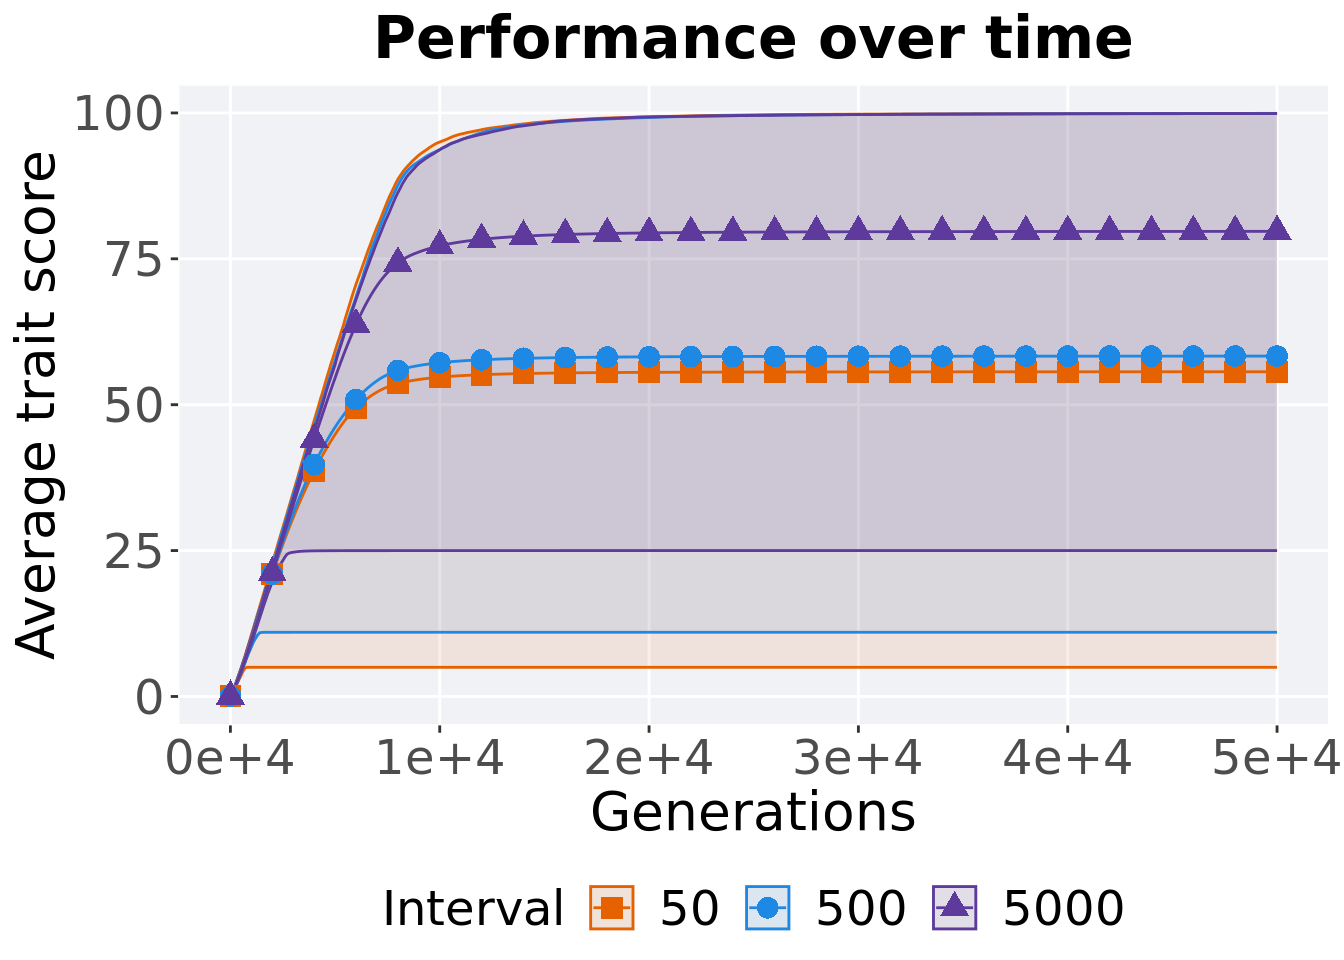
\includegraphics{demo_files/figure-latex/int-tru-mpe-perf-1.pdf}

\hypertarget{best-performance}{%
\subsubsection{Best performance}\label{best-performance}}

Best performancefound throughout the 50,000 generations.

\begin{Shaded}
\begin{Highlighting}[]
\KeywordTok{filter}\NormalTok{(df_best, Diagnostic }\OperatorTok{==}\StringTok{ 'MULTIPATH_EXPLORATION'} \OperatorTok{&}\StringTok{ `}\DataTypeTok{Selection}\CharTok{\textbackslash{}n}\DataTypeTok{Scheme}\StringTok{`} \OperatorTok{==}\StringTok{ 'TRUNCATION'} \OperatorTok{&}\StringTok{ }\NormalTok{VAR }\OperatorTok{==}\StringTok{ 'pop_fit_max'}\NormalTok{) }\OperatorTok
\StringTok{  }\KeywordTok{ggplot}\NormalTok{(., }\KeywordTok{aes}\NormalTok{(}\DataTypeTok{x =}\NormalTok{ Interval, }\DataTypeTok{y =}\NormalTok{ VAL }\OperatorTok{/}\StringTok{ }\NormalTok{DIMENSIONALITY, }\DataTypeTok{color =}\NormalTok{ Interval, }\DataTypeTok{fill =}\NormalTok{ Interval, }\DataTypeTok{shape =}\NormalTok{ Interval)) }\OperatorTok{+}
\StringTok{  }\KeywordTok{geom_flat_violin}\NormalTok{(}\DataTypeTok{position =} \KeywordTok{position_nudge}\NormalTok{(}\DataTypeTok{x =} \FloatTok{.2}\NormalTok{, }\DataTypeTok{y =} \DecValTok{0}\NormalTok{), }\DataTypeTok{scale =} \StringTok{'width'}\NormalTok{, }\DataTypeTok{alpha =} \FloatTok{0.2}\NormalTok{) }\OperatorTok{+}
\StringTok{  }\KeywordTok{geom_point}\NormalTok{(}\DataTypeTok{position =} \KeywordTok{position_jitter}\NormalTok{(}\DataTypeTok{width =} \FloatTok{.1}\NormalTok{), }\DataTypeTok{size =} \FloatTok{1.5}\NormalTok{, }\DataTypeTok{alpha =} \FloatTok{1.0}\NormalTok{) }\OperatorTok{+}
\StringTok{  }\KeywordTok{geom_boxplot}\NormalTok{(}\DataTypeTok{color =} \StringTok{'black'}\NormalTok{, }\DataTypeTok{width =} \FloatTok{.2}\NormalTok{, }\DataTypeTok{outlier.shape =} \OtherTok{NA}\NormalTok{, }\DataTypeTok{alpha =} \FloatTok{0.0}\NormalTok{) }\OperatorTok{+}
\StringTok{  }\KeywordTok{scale_y_continuous}\NormalTok{(}
    \DataTypeTok{name=}\StringTok{"Average trait score"}
\NormalTok{  ) }\OperatorTok{+}
\StringTok{  }\KeywordTok{scale_x_discrete}\NormalTok{(}
    \DataTypeTok{name=}\StringTok{"Interval"}
\NormalTok{  )}\OperatorTok{+}
\StringTok{  }\KeywordTok{scale_shape_manual}\NormalTok{(}\DataTypeTok{values=}\NormalTok{SHAPE)}\OperatorTok{+}
\StringTok{  }\KeywordTok{scale_colour_manual}\NormalTok{(}\DataTypeTok{values =}\NormalTok{ cb_palette_mi, ) }\OperatorTok{+}
\StringTok{  }\KeywordTok{scale_fill_manual}\NormalTok{(}\DataTypeTok{values =}\NormalTok{ cb_palette_mi) }\OperatorTok{+}
\StringTok{  }\KeywordTok{ggtitle}\NormalTok{(}\StringTok{'Best performance'}\NormalTok{)}\OperatorTok{+}
\StringTok{  }\NormalTok{p_theme }\OperatorTok{+}\StringTok{ }\KeywordTok{coord_flip}\NormalTok{()}
\end{Highlighting}
\end{Shaded}

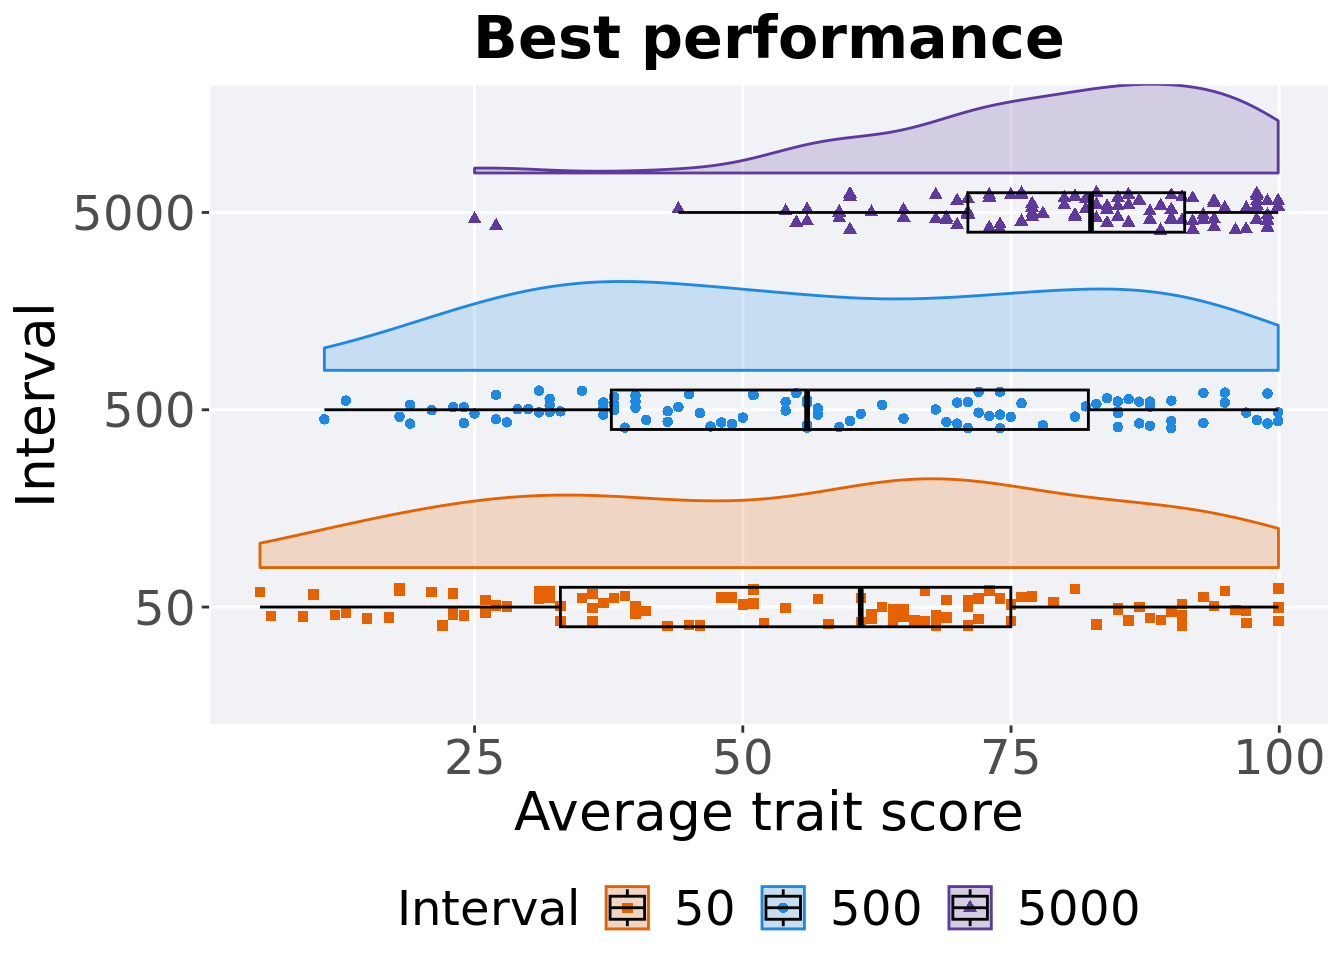
\includegraphics{demo_files/figure-latex/int-tru-mpe-per-bst-1.pdf}

\hypertarget{stats-16}{%
\paragraph{Stats}\label{stats-16}}

Summary statistics for the first generation a best performance found.

\begin{Shaded}
\begin{Highlighting}[]
\NormalTok{performance =}\StringTok{ }\KeywordTok{filter}\NormalTok{(df_best, Diagnostic }\OperatorTok{==}\StringTok{ 'MULTIPATH_EXPLORATION'} \OperatorTok{&}\StringTok{ `}\DataTypeTok{Selection}\CharTok{\textbackslash{}n}\DataTypeTok{Scheme}\StringTok{`} \OperatorTok{==}\StringTok{ 'TRUNCATION'} \OperatorTok{&}\StringTok{ }\NormalTok{VAR }\OperatorTok{==}\StringTok{ 'pop_fit_max'}\NormalTok{)}
\NormalTok{performance }\OperatorTok
\StringTok{  }\KeywordTok{group_by}\NormalTok{(Interval) }\OperatorTok
\StringTok{  }\NormalTok{dplyr}\OperatorTok{::}\KeywordTok{summarise}\NormalTok{(}
    \DataTypeTok{count =} \KeywordTok{n}\NormalTok{(),}
    \DataTypeTok{na_cnt =} \KeywordTok{sum}\NormalTok{(}\KeywordTok{is.na}\NormalTok{(VAL)),}
    \DataTypeTok{min =} \KeywordTok{min}\NormalTok{(VAL, }\DataTypeTok{na.rm =} \OtherTok{TRUE}\NormalTok{) }\OperatorTok{/}\StringTok{ }\NormalTok{DIMENSIONALITY,}
    \DataTypeTok{median =} \KeywordTok{median}\NormalTok{(VAL, }\DataTypeTok{na.rm =} \OtherTok{TRUE}\NormalTok{) }\OperatorTok{/}\StringTok{ }\NormalTok{DIMENSIONALITY,}
    \DataTypeTok{mean =} \KeywordTok{mean}\NormalTok{(VAL, }\DataTypeTok{na.rm =} \OtherTok{TRUE}\NormalTok{) }\OperatorTok{/}\StringTok{ }\NormalTok{DIMENSIONALITY,}
    \DataTypeTok{max =} \KeywordTok{max}\NormalTok{(VAL, }\DataTypeTok{na.rm =} \OtherTok{TRUE}\NormalTok{) }\OperatorTok{/}\StringTok{ }\NormalTok{DIMENSIONALITY,}
    \DataTypeTok{IQR =} \KeywordTok{IQR}\NormalTok{(VAL, }\DataTypeTok{na.rm =} \OtherTok{TRUE}\NormalTok{) }\OperatorTok{/}\StringTok{ }\NormalTok{DIMENSIONALITY}
\NormalTok{  )}
\end{Highlighting}
\end{Shaded}

\begin{verbatim}
## # A tibble: 3 x 8
##   Interval count na_cnt   min median  mean   max   IQR
##   <fct>    <int>  <int> <dbl>  <dbl> <dbl> <dbl> <dbl>
## 1 50         100      0   5     61.0  55.6  99.9  42.0
## 2 500        100      0  11     56.0  58.3  99.9  44.5
## 3 5000       100      0  25.0   82.5  79.7  99.9  20.2
\end{verbatim}

Kruskal--Wallis test provides evidence of difference among selection schemes.

\begin{Shaded}
\begin{Highlighting}[]
\KeywordTok{kruskal.test}\NormalTok{(VAL }\OperatorTok{~}\StringTok{ }\NormalTok{Interval, }\DataTypeTok{data =}\NormalTok{ performance)}
\end{Highlighting}
\end{Shaded}

\begin{verbatim}
## 
##  Kruskal-Wallis rank sum test
## 
## data:  VAL by Interval
## Kruskal-Wallis chi-squared = 51.085, df = 2, p-value = 8.073e-12
\end{verbatim}

Results for post-hoc Wilcoxon rank-sum test with a Bonferroni correction.

\begin{Shaded}
\begin{Highlighting}[]
\KeywordTok{pairwise.wilcox.test}\NormalTok{(}\DataTypeTok{x =}\NormalTok{ performance}\OperatorTok{$}\NormalTok{VAL, }\DataTypeTok{g =}\NormalTok{ performance}\OperatorTok{$}\NormalTok{Interval, }\DataTypeTok{p.adjust.method =} \StringTok{"bonferroni"}\NormalTok{,}
                     \DataTypeTok{paired =} \OtherTok{FALSE}\NormalTok{, }\DataTypeTok{conf.int =} \OtherTok{FALSE}\NormalTok{, }\DataTypeTok{alternative =} \StringTok{'g'}\NormalTok{)}
\end{Highlighting}
\end{Shaded}

\begin{verbatim}
## 
##  Pairwise comparisons using Wilcoxon rank sum test with continuity correction 
## 
## data:  performance$VAL and performance$Interval 
## 
##      50      500    
## 500  0.87    -      
## 5000 1.9e-10 5.5e-09
## 
## P value adjustment method: bonferroni
\end{verbatim}

\hypertarget{final-performance}{%
\subsubsection{Final performance}\label{final-performance}}

Best performance is found throughout in final generation.

\begin{Shaded}
\begin{Highlighting}[]
\KeywordTok{filter}\NormalTok{(df_ot, Diagnostic }\OperatorTok{==}\StringTok{ 'MULTIPATH_EXPLORATION'} \OperatorTok{&}\StringTok{ `}\DataTypeTok{Selection}\CharTok{\textbackslash{}n}\DataTypeTok{Scheme}\StringTok{`} \OperatorTok{==}\StringTok{ 'TRUNCATION'} \OperatorTok{&}\StringTok{ }\NormalTok{Generations }\OperatorTok{==}\StringTok{ }\DecValTok{50000}\NormalTok{) }\OperatorTok
\StringTok{  }\KeywordTok{ggplot}\NormalTok{(., }\KeywordTok{aes}\NormalTok{(}\DataTypeTok{x =}\NormalTok{ Interval, }\DataTypeTok{y =}\NormalTok{ pop_fit_max }\OperatorTok{/}\StringTok{ }\NormalTok{DIMENSIONALITY, }\DataTypeTok{color =}\NormalTok{ Interval, }\DataTypeTok{fill =}\NormalTok{ Interval, }\DataTypeTok{shape =}\NormalTok{ Interval)) }\OperatorTok{+}
\StringTok{  }\KeywordTok{geom_flat_violin}\NormalTok{(}\DataTypeTok{position =} \KeywordTok{position_nudge}\NormalTok{(}\DataTypeTok{x =} \FloatTok{.2}\NormalTok{, }\DataTypeTok{y =} \DecValTok{0}\NormalTok{), }\DataTypeTok{scale =} \StringTok{'width'}\NormalTok{, }\DataTypeTok{alpha =} \FloatTok{0.2}\NormalTok{) }\OperatorTok{+}
\StringTok{  }\KeywordTok{geom_point}\NormalTok{(}\DataTypeTok{position =} \KeywordTok{position_jitter}\NormalTok{(}\DataTypeTok{width =} \FloatTok{.1}\NormalTok{), }\DataTypeTok{size =} \FloatTok{1.5}\NormalTok{, }\DataTypeTok{alpha =} \FloatTok{1.0}\NormalTok{) }\OperatorTok{+}
\StringTok{  }\KeywordTok{geom_boxplot}\NormalTok{(}\DataTypeTok{color =} \StringTok{'black'}\NormalTok{, }\DataTypeTok{width =} \FloatTok{.2}\NormalTok{, }\DataTypeTok{outlier.shape =} \OtherTok{NA}\NormalTok{, }\DataTypeTok{alpha =} \FloatTok{0.0}\NormalTok{) }\OperatorTok{+}
\StringTok{  }\KeywordTok{scale_y_continuous}\NormalTok{(}
    \DataTypeTok{name=}\StringTok{"Average trait score"}
\NormalTok{  ) }\OperatorTok{+}
\StringTok{  }\KeywordTok{scale_x_discrete}\NormalTok{(}
    \DataTypeTok{name=}\StringTok{"Interval"}
\NormalTok{  )}\OperatorTok{+}
\StringTok{  }\KeywordTok{scale_shape_manual}\NormalTok{(}\DataTypeTok{values=}\NormalTok{SHAPE)}\OperatorTok{+}
\StringTok{  }\KeywordTok{scale_colour_manual}\NormalTok{(}\DataTypeTok{values =}\NormalTok{ cb_palette_mi, ) }\OperatorTok{+}
\StringTok{  }\KeywordTok{scale_fill_manual}\NormalTok{(}\DataTypeTok{values =}\NormalTok{ cb_palette_mi) }\OperatorTok{+}
\StringTok{  }\KeywordTok{ggtitle}\NormalTok{(}\StringTok{'Final performance'}\NormalTok{)}\OperatorTok{+}
\StringTok{  }\NormalTok{p_theme }\OperatorTok{+}\StringTok{ }\KeywordTok{coord_flip}\NormalTok{()}
\end{Highlighting}
\end{Shaded}

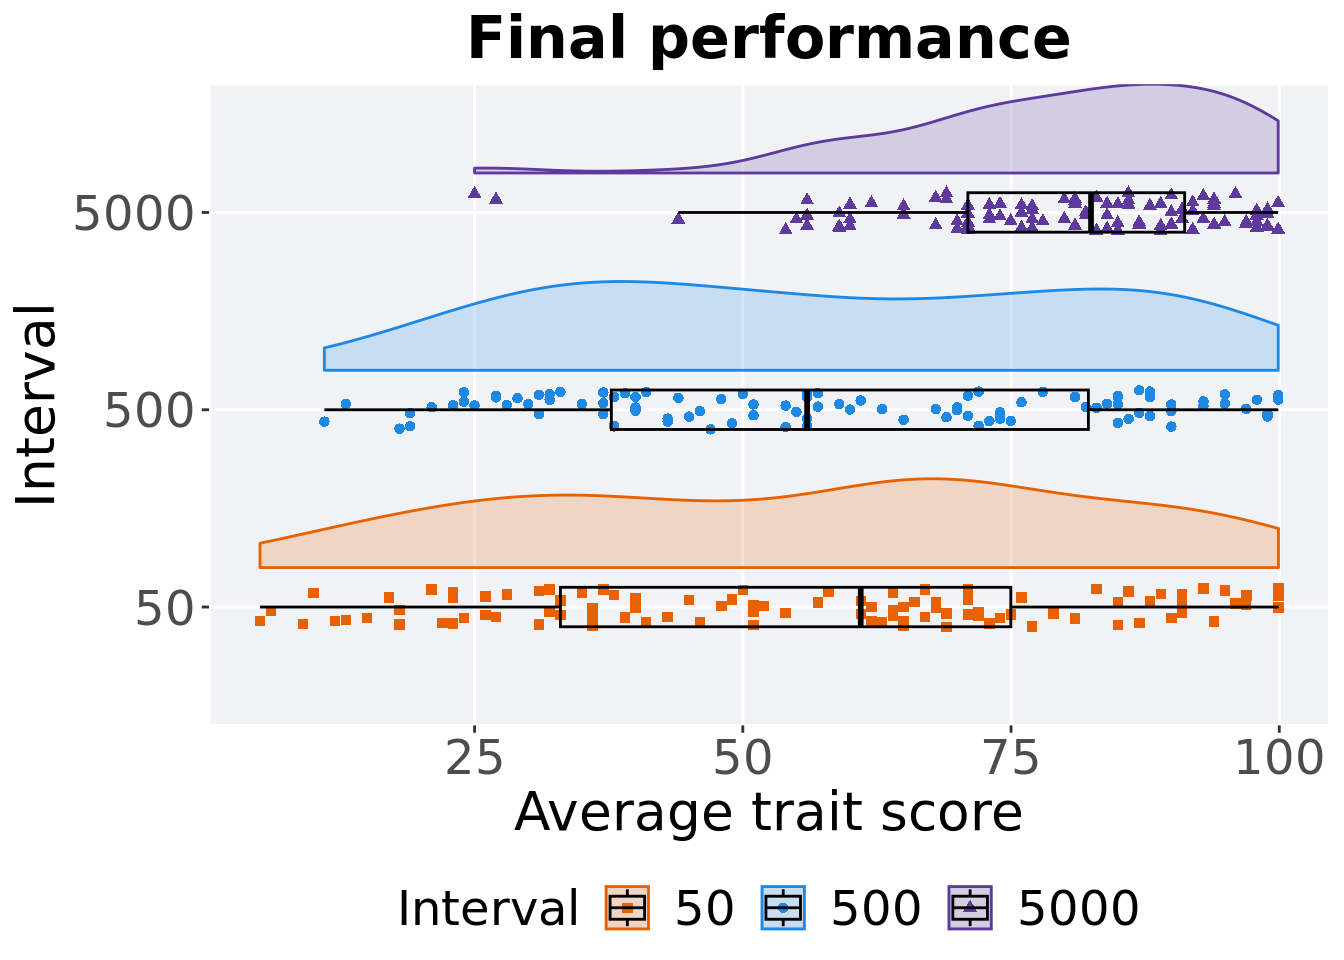
\includegraphics{demo_files/figure-latex/int-tru-mpe-per-end-1.pdf}

\hypertarget{stats-17}{%
\paragraph{Stats}\label{stats-17}}

Summary statistics for the best performance is found in final generation.

\begin{Shaded}
\begin{Highlighting}[]
\NormalTok{performance =}\StringTok{ }\KeywordTok{filter}\NormalTok{(df_ot, Diagnostic }\OperatorTok{==}\StringTok{ 'MULTIPATH_EXPLORATION'} \OperatorTok{&}\StringTok{ `}\DataTypeTok{Selection}\CharTok{\textbackslash{}n}\DataTypeTok{Scheme}\StringTok{`} \OperatorTok{==}\StringTok{ 'TRUNCATION'} \OperatorTok{&}\StringTok{ }\NormalTok{Generations }\OperatorTok{==}\StringTok{ }\DecValTok{50000}\NormalTok{)}
\NormalTok{performance }\OperatorTok
\StringTok{  }\KeywordTok{group_by}\NormalTok{(Interval) }\OperatorTok
\StringTok{  }\NormalTok{dplyr}\OperatorTok{::}\KeywordTok{summarise}\NormalTok{(}
    \DataTypeTok{count =} \KeywordTok{n}\NormalTok{(),}
    \DataTypeTok{na_cnt =} \KeywordTok{sum}\NormalTok{(}\KeywordTok{is.na}\NormalTok{(pop_fit_max)),}
    \DataTypeTok{min =} \KeywordTok{min}\NormalTok{(pop_fit_max }\OperatorTok{/}\StringTok{ }\NormalTok{DIMENSIONALITY, }\DataTypeTok{na.rm =} \OtherTok{TRUE}\NormalTok{),}
    \DataTypeTok{median =} \KeywordTok{median}\NormalTok{(pop_fit_max }\OperatorTok{/}\StringTok{ }\NormalTok{DIMENSIONALITY, }\DataTypeTok{na.rm =} \OtherTok{TRUE}\NormalTok{),}
    \DataTypeTok{mean =} \KeywordTok{mean}\NormalTok{(pop_fit_max }\OperatorTok{/}\StringTok{ }\NormalTok{DIMENSIONALITY, }\DataTypeTok{na.rm =} \OtherTok{TRUE}\NormalTok{),}
    \DataTypeTok{max =} \KeywordTok{max}\NormalTok{(pop_fit_max }\OperatorTok{/}\StringTok{ }\NormalTok{DIMENSIONALITY, }\DataTypeTok{na.rm =} \OtherTok{TRUE}\NormalTok{),}
    \DataTypeTok{IQR =} \KeywordTok{IQR}\NormalTok{(pop_fit_max }\OperatorTok{/}\StringTok{ }\NormalTok{DIMENSIONALITY, }\DataTypeTok{na.rm =} \OtherTok{TRUE}\NormalTok{)}
\NormalTok{  )}
\end{Highlighting}
\end{Shaded}

\begin{verbatim}
## # A tibble: 3 x 8
##   Interval count na_cnt   min median  mean   max   IQR
##   <fct>    <int>  <int> <dbl>  <dbl> <dbl> <dbl> <dbl>
## 1 50         100      0   5     61.0  55.6  99.9  42.0
## 2 500        100      0  11     56.0  58.3  99.9  44.5
## 3 5000       100      0  25.0   82.5  79.7  99.9  20.2
\end{verbatim}

Kruskal--Wallis test provides evidence of difference among selection schemes.

\begin{Shaded}
\begin{Highlighting}[]
\KeywordTok{kruskal.test}\NormalTok{(pop_fit_max }\OperatorTok{~}\StringTok{ }\NormalTok{Interval, }\DataTypeTok{data =}\NormalTok{ performance)}
\end{Highlighting}
\end{Shaded}

\begin{verbatim}
## 
##  Kruskal-Wallis rank sum test
## 
## data:  pop_fit_max by Interval
## Kruskal-Wallis chi-squared = 51.085, df = 2, p-value = 8.073e-12
\end{verbatim}

Results for post-hoc Wilcoxon rank-sum test with a Bonferroni correction.

\begin{Shaded}
\begin{Highlighting}[]
\KeywordTok{pairwise.wilcox.test}\NormalTok{(}\DataTypeTok{x =}\NormalTok{ performance}\OperatorTok{$}\NormalTok{pop_fit_max, }\DataTypeTok{g =}\NormalTok{ performance}\OperatorTok{$}\NormalTok{Interval, }\DataTypeTok{p.adjust.method =} \StringTok{"bonferroni"}\NormalTok{,}
                     \DataTypeTok{paired =} \OtherTok{FALSE}\NormalTok{, }\DataTypeTok{conf.int =} \OtherTok{FALSE}\NormalTok{, }\DataTypeTok{alternative =} \StringTok{'g'}\NormalTok{)}
\end{Highlighting}
\end{Shaded}

\begin{verbatim}
## 
##  Pairwise comparisons using Wilcoxon rank sum test with continuity correction 
## 
## data:  performance$pop_fit_max and performance$Interval 
## 
##      50      500    
## 500  0.87    -      
## 5000 1.9e-10 5.5e-09
## 
## P value adjustment method: bonferroni
\end{verbatim}

\hypertarget{activation-gene-coverage-3}{%
\subsection{Activation gene coverage}\label{activation-gene-coverage-3}}

Activation gene coverage analysis.

\hypertarget{coverage-over-time-6}{%
\subsubsection{Coverage over time}\label{coverage-over-time-6}}

Activation gene coverage over time.

\begin{Shaded}
\begin{Highlighting}[]
\CommentTok{# data for lines and shading on plots}
\NormalTok{lines =}\StringTok{ }\KeywordTok{filter}\NormalTok{(df_ot, Diagnostic }\OperatorTok{==}\StringTok{ 'MULTIPATH_EXPLORATION'} \OperatorTok{&}\StringTok{ `}\DataTypeTok{Selection}\CharTok{\textbackslash{}n}\DataTypeTok{Scheme}\StringTok{`} \OperatorTok{==}\StringTok{ 'TRUNCATION'}\NormalTok{) }\OperatorTok
\StringTok{  }\KeywordTok{group_by}\NormalTok{(Interval, Generations) }\OperatorTok
\StringTok{  }\NormalTok{dplyr}\OperatorTok{::}\KeywordTok{summarise}\NormalTok{(}
    \DataTypeTok{min =} \KeywordTok{min}\NormalTok{(pop_act_cov),}
    \DataTypeTok{mean =} \KeywordTok{mean}\NormalTok{(pop_act_cov),}
    \DataTypeTok{max =} \KeywordTok{max}\NormalTok{(pop_act_cov)}
\NormalTok{  )}
\end{Highlighting}
\end{Shaded}

\begin{verbatim}
## `summarise()` has grouped output by 'Interval'. You can override using the
## `.groups` argument.
\end{verbatim}

\begin{Shaded}
\begin{Highlighting}[]
\KeywordTok{ggplot}\NormalTok{(lines, }\KeywordTok{aes}\NormalTok{(}\DataTypeTok{x=}\NormalTok{Generations, }\DataTypeTok{y=}\NormalTok{mean, }\DataTypeTok{group =}\NormalTok{ Interval, }\DataTypeTok{fill =}\NormalTok{ Interval, }\DataTypeTok{color =}\NormalTok{ Interval, }\DataTypeTok{shape =}\NormalTok{ Interval)) }\OperatorTok{+}
\StringTok{  }\KeywordTok{geom_ribbon}\NormalTok{(}\KeywordTok{aes}\NormalTok{(}\DataTypeTok{ymin =}\NormalTok{ min, }\DataTypeTok{ymax =}\NormalTok{ max), }\DataTypeTok{alpha =} \FloatTok{0.1}\NormalTok{) }\OperatorTok{+}
\StringTok{  }\KeywordTok{geom_line}\NormalTok{(}\DataTypeTok{size =} \FloatTok{0.5}\NormalTok{) }\OperatorTok{+}
\StringTok{  }\KeywordTok{geom_point}\NormalTok{(}\DataTypeTok{data =} \KeywordTok{filter}\NormalTok{(lines, Generations }\OperatorTok\StringTok{ }\DecValTok{2000} \OperatorTok{==}\StringTok{ }\DecValTok{0}\NormalTok{), }\DataTypeTok{size =} \FloatTok{1.5}\NormalTok{, }\DataTypeTok{stroke =} \FloatTok{2.0}\NormalTok{, }\DataTypeTok{alpha =} \FloatTok{1.0}\NormalTok{) }\OperatorTok{+}
\StringTok{  }\KeywordTok{scale_y_continuous}\NormalTok{(}
    \DataTypeTok{name=}\StringTok{"Coverage"}
\NormalTok{  ) }\OperatorTok{+}
\StringTok{  }\KeywordTok{scale_x_continuous}\NormalTok{(}
    \DataTypeTok{name=}\StringTok{"Generations"}\NormalTok{,}
    \DataTypeTok{limits=}\KeywordTok{c}\NormalTok{(}\DecValTok{0}\NormalTok{, }\DecValTok{50000}\NormalTok{),}
    \DataTypeTok{breaks=}\KeywordTok{c}\NormalTok{(}\DecValTok{0}\NormalTok{, }\DecValTok{10000}\NormalTok{, }\DecValTok{20000}\NormalTok{, }\DecValTok{30000}\NormalTok{, }\DecValTok{40000}\NormalTok{, }\DecValTok{50000}\NormalTok{),}
    \DataTypeTok{labels=}\KeywordTok{c}\NormalTok{(}\StringTok{"0e+4"}\NormalTok{, }\StringTok{"1e+4"}\NormalTok{, }\StringTok{"2e+4"}\NormalTok{, }\StringTok{"3e+4"}\NormalTok{, }\StringTok{"4e+4"}\NormalTok{, }\StringTok{"5e+4"}\NormalTok{)}

\NormalTok{  ) }\OperatorTok{+}
\StringTok{  }\KeywordTok{scale_shape_manual}\NormalTok{(}\DataTypeTok{values=}\NormalTok{SHAPE)}\OperatorTok{+}
\StringTok{  }\KeywordTok{scale_colour_manual}\NormalTok{(}\DataTypeTok{values =}\NormalTok{ cb_palette_mi) }\OperatorTok{+}
\StringTok{  }\KeywordTok{scale_fill_manual}\NormalTok{(}\DataTypeTok{values =}\NormalTok{ cb_palette_mi) }\OperatorTok{+}
\StringTok{  }\KeywordTok{ggtitle}\NormalTok{(}\StringTok{'Activation gene coverage over time'}\NormalTok{)}\OperatorTok{+}
\StringTok{  }\NormalTok{p_theme}
\end{Highlighting}
\end{Shaded}

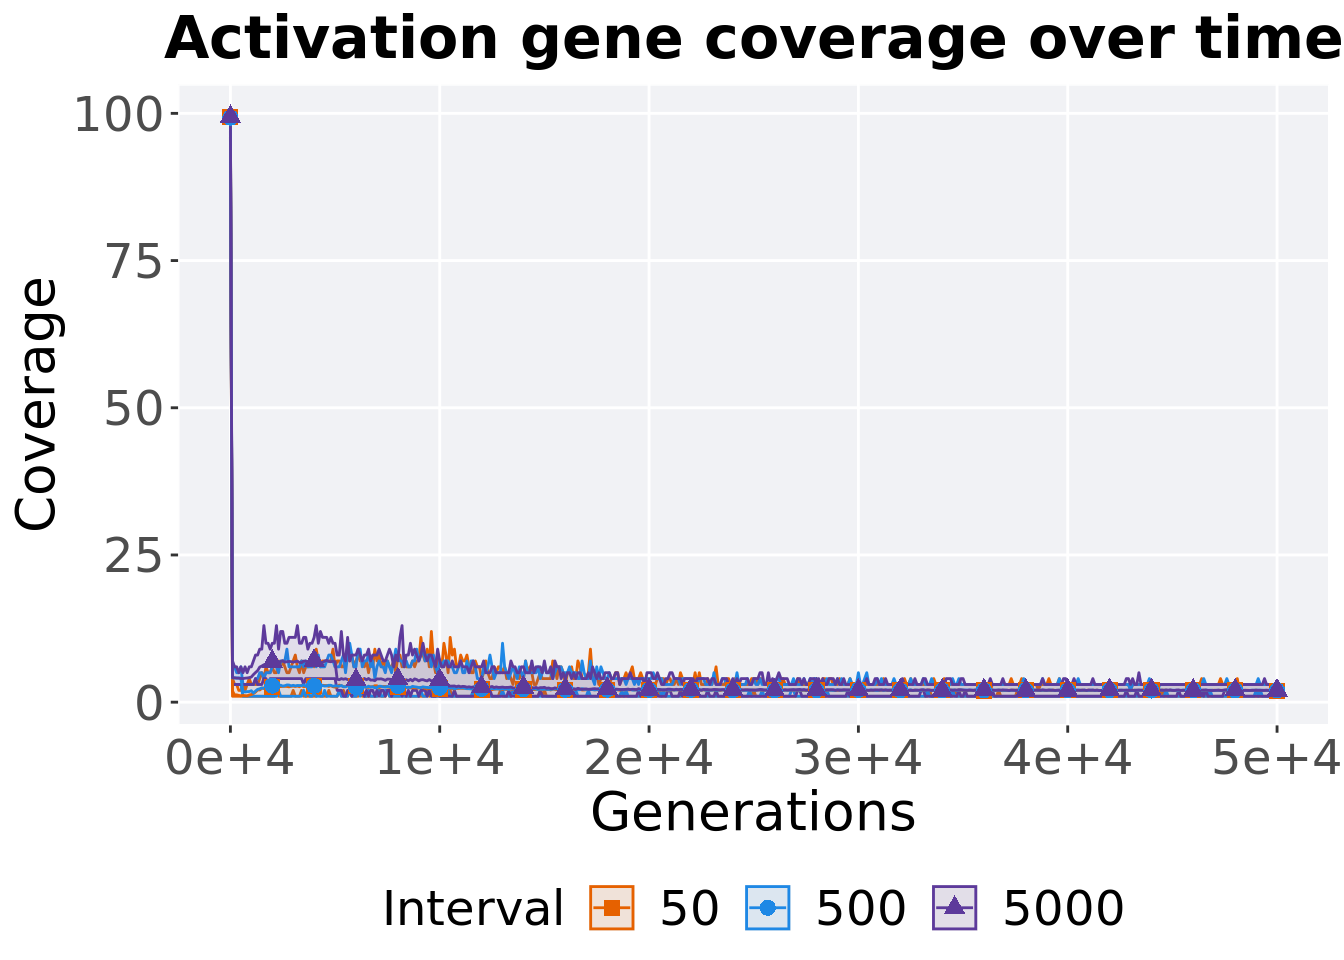
\includegraphics{demo_files/figure-latex/int-mpe-act-tru-ot-1.pdf}

\hypertarget{end-of-50000-generations-6}{%
\subsubsection{End of 50,000 generations}\label{end-of-50000-generations-6}}

Activation gene coverage in the population at the end of 50,000 generations.

\begin{Shaded}
\begin{Highlighting}[]
\CommentTok{### end of run}
\KeywordTok{filter}\NormalTok{(df_ot, Diagnostic }\OperatorTok{==}\StringTok{ 'MULTIPATH_EXPLORATION'} \OperatorTok{&}\StringTok{ `}\DataTypeTok{Selection}\CharTok{\textbackslash{}n}\DataTypeTok{Scheme}\StringTok{`} \OperatorTok{==}\StringTok{ 'TRUNCATION'} \OperatorTok{&}\StringTok{ }\NormalTok{Generations }\OperatorTok{==}\StringTok{ }\DecValTok{50000}\NormalTok{) }\OperatorTok
\StringTok{  }\KeywordTok{ggplot}\NormalTok{(., }\KeywordTok{aes}\NormalTok{(}\DataTypeTok{x =}\NormalTok{ Interval, }\DataTypeTok{y =}\NormalTok{ pop_act_cov, }\DataTypeTok{color =}\NormalTok{ Interval, }\DataTypeTok{fill =}\NormalTok{ Interval, }\DataTypeTok{shape =}\NormalTok{ Interval)) }\OperatorTok{+}
\StringTok{  }\KeywordTok{geom_flat_violin}\NormalTok{(}\DataTypeTok{position =} \KeywordTok{position_nudge}\NormalTok{(}\DataTypeTok{x =} \FloatTok{.2}\NormalTok{, }\DataTypeTok{y =} \DecValTok{0}\NormalTok{), }\DataTypeTok{scale =} \StringTok{'width'}\NormalTok{, }\DataTypeTok{alpha =} \FloatTok{0.3}\NormalTok{) }\OperatorTok{+}
\StringTok{  }\KeywordTok{geom_point}\NormalTok{(}\DataTypeTok{position =} \KeywordTok{position_jitter}\NormalTok{(}\DataTypeTok{height =} \FloatTok{.05}\NormalTok{, }\DataTypeTok{width =} \FloatTok{.05}\NormalTok{), }\DataTypeTok{size =} \FloatTok{1.5}\NormalTok{, }\DataTypeTok{alpha =} \FloatTok{0.5}\NormalTok{) }\OperatorTok{+}
\StringTok{  }\KeywordTok{geom_boxplot}\NormalTok{(}\DataTypeTok{color =} \StringTok{'black'}\NormalTok{, }\DataTypeTok{width =} \FloatTok{.2}\NormalTok{, }\DataTypeTok{outlier.shape =} \OtherTok{NA}\NormalTok{, }\DataTypeTok{alpha =} \FloatTok{0.0}\NormalTok{) }\OperatorTok{+}
\StringTok{  }\KeywordTok{scale_shape_manual}\NormalTok{(}\DataTypeTok{values=}\NormalTok{SHAPE)}\OperatorTok{+}
\StringTok{  }\KeywordTok{scale_y_continuous}\NormalTok{(}
    \DataTypeTok{name=}\StringTok{"Coverage"}
\NormalTok{  ) }\OperatorTok{+}
\StringTok{  }\KeywordTok{scale_x_discrete}\NormalTok{(}
    \DataTypeTok{name=}\StringTok{"Interval"}
\NormalTok{  ) }\OperatorTok{+}
\StringTok{  }\KeywordTok{scale_colour_manual}\NormalTok{(}\DataTypeTok{values =}\NormalTok{ cb_palette_mi) }\OperatorTok{+}
\StringTok{  }\KeywordTok{scale_fill_manual}\NormalTok{(}\DataTypeTok{values =}\NormalTok{ cb_palette_mi) }\OperatorTok{+}
\StringTok{  }\KeywordTok{ggtitle}\NormalTok{(}\StringTok{'Final activation gene coverage'}\NormalTok{)}\OperatorTok{+}
\StringTok{  }\NormalTok{p_theme }\OperatorTok{+}\StringTok{ }\KeywordTok{coord_flip}\NormalTok{()}
\end{Highlighting}
\end{Shaded}

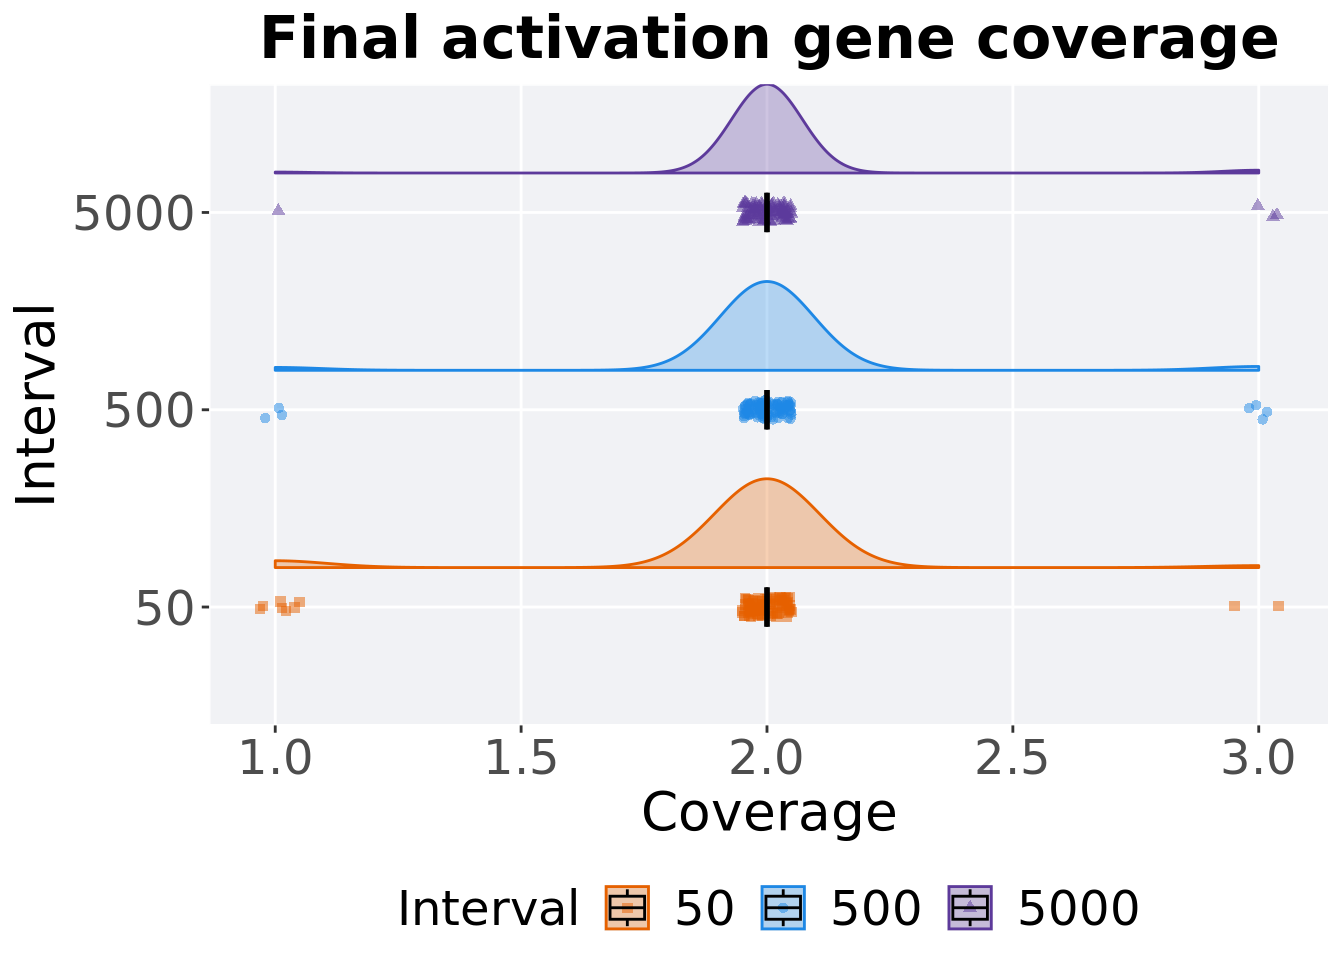
\includegraphics{demo_files/figure-latex/int-mpe-act-tru-end-1.pdf}

\hypertarget{stats-18}{%
\paragraph{Stats}\label{stats-18}}

Summary statistics for activation gene coverage.

\begin{Shaded}
\begin{Highlighting}[]
\NormalTok{coverage =}\StringTok{ }\KeywordTok{filter}\NormalTok{(df_ot, Diagnostic }\OperatorTok{==}\StringTok{ 'MULTIPATH_EXPLORATION'} \OperatorTok{&}\StringTok{ `}\DataTypeTok{Selection}\CharTok{\textbackslash{}n}\DataTypeTok{Scheme}\StringTok{`} \OperatorTok{==}\StringTok{ 'TRUNCATION'} \OperatorTok{&}\StringTok{ }\NormalTok{Generations }\OperatorTok{==}\StringTok{ }\DecValTok{50000}\NormalTok{)}
\NormalTok{coverage }\OperatorTok
\StringTok{  }\KeywordTok{group_by}\NormalTok{(Interval) }\OperatorTok
\StringTok{  }\NormalTok{dplyr}\OperatorTok{::}\KeywordTok{summarise}\NormalTok{(}
    \DataTypeTok{count =} \KeywordTok{n}\NormalTok{(),}
    \DataTypeTok{na_cnt =} \KeywordTok{sum}\NormalTok{(}\KeywordTok{is.na}\NormalTok{(pop_act_cov)),}
    \DataTypeTok{min =} \KeywordTok{min}\NormalTok{(pop_act_cov, }\DataTypeTok{na.rm =} \OtherTok{TRUE}\NormalTok{),}
    \DataTypeTok{median =} \KeywordTok{median}\NormalTok{(pop_act_cov, }\DataTypeTok{na.rm =} \OtherTok{TRUE}\NormalTok{),}
    \DataTypeTok{mean =} \KeywordTok{mean}\NormalTok{(pop_act_cov, }\DataTypeTok{na.rm =} \OtherTok{TRUE}\NormalTok{),}
    \DataTypeTok{max =} \KeywordTok{max}\NormalTok{(pop_act_cov, }\DataTypeTok{na.rm =} \OtherTok{TRUE}\NormalTok{),}
    \DataTypeTok{IQR =} \KeywordTok{IQR}\NormalTok{(pop_act_cov, }\DataTypeTok{na.rm =} \OtherTok{TRUE}\NormalTok{)}
\NormalTok{  )}
\end{Highlighting}
\end{Shaded}

\begin{verbatim}
## # A tibble: 3 x 8
##   Interval count na_cnt   min median  mean   max   IQR
##   <fct>    <int>  <int> <int>  <dbl> <dbl> <int> <dbl>
## 1 50         100      0     1      2  1.95     3     0
## 2 500        100      0     1      2  2.01     3     0
## 3 5000       100      0     1      2  2.02     3     0
\end{verbatim}

Kruskal--Wallis test provides evidence of no difference among activation gene coverage.

\begin{Shaded}
\begin{Highlighting}[]
\KeywordTok{kruskal.test}\NormalTok{(pop_act_cov }\OperatorTok{~}\StringTok{ }\NormalTok{Interval, }\DataTypeTok{data =}\NormalTok{ coverage)}
\end{Highlighting}
\end{Shaded}

\begin{verbatim}
## 
##  Kruskal-Wallis rank sum test
## 
## data:  pop_act_cov by Interval
## Kruskal-Wallis chi-squared = 4.3029, df = 2, p-value = 0.1163
\end{verbatim}

\hypertarget{tournament-selection-3}{%
\section{Tournament selection}\label{tournament-selection-3}}

Here we analyze how the different population structures affect tournament selection (size 8) on the contradictory objectives diagnostic.

\hypertarget{performance-1}{%
\subsection{Performance}\label{performance-1}}

\hypertarget{performance-over-time-7}{%
\subsubsection{Performance over time}\label{performance-over-time-7}}

\begin{Shaded}
\begin{Highlighting}[]
\NormalTok{lines =}\StringTok{ }\KeywordTok{filter}\NormalTok{(df_ot, Diagnostic }\OperatorTok{==}\StringTok{ 'MULTIPATH_EXPLORATION'} \OperatorTok{&}\StringTok{ `}\DataTypeTok{Selection}\CharTok{\textbackslash{}n}\DataTypeTok{Scheme}\StringTok{`} \OperatorTok{==}\StringTok{ 'TOURNAMENT'}\NormalTok{) }\OperatorTok
\StringTok{  }\KeywordTok{group_by}\NormalTok{(Interval, Generations) }\OperatorTok
\StringTok{  }\NormalTok{dplyr}\OperatorTok{::}\KeywordTok{summarise}\NormalTok{(}
    \DataTypeTok{min =} \KeywordTok{min}\NormalTok{(pop_fit_max) }\OperatorTok{/}\StringTok{ }\NormalTok{DIMENSIONALITY,}
    \DataTypeTok{mean =} \KeywordTok{mean}\NormalTok{(pop_fit_max) }\OperatorTok{/}\StringTok{ }\NormalTok{DIMENSIONALITY,}
    \DataTypeTok{max =} \KeywordTok{max}\NormalTok{(pop_fit_max) }\OperatorTok{/}\StringTok{ }\NormalTok{DIMENSIONALITY}
\NormalTok{  )}
\KeywordTok{ggplot}\NormalTok{(lines, }\KeywordTok{aes}\NormalTok{(}\DataTypeTok{x=}\NormalTok{Generations, }\DataTypeTok{y=}\NormalTok{mean, }\DataTypeTok{group =}\NormalTok{ Interval, }\DataTypeTok{fill =}\NormalTok{ Interval, }\DataTypeTok{color =}\NormalTok{ Interval, }\DataTypeTok{shape =}\NormalTok{ Interval)) }\OperatorTok{+}
\StringTok{  }\KeywordTok{geom_ribbon}\NormalTok{(}\KeywordTok{aes}\NormalTok{(}\DataTypeTok{ymin =}\NormalTok{ min, }\DataTypeTok{ymax =}\NormalTok{ max), }\DataTypeTok{alpha =} \FloatTok{0.1}\NormalTok{) }\OperatorTok{+}
\StringTok{  }\KeywordTok{geom_line}\NormalTok{(}\DataTypeTok{size =} \FloatTok{0.5}\NormalTok{) }\OperatorTok{+}
\StringTok{  }\KeywordTok{geom_point}\NormalTok{(}\DataTypeTok{data =} \KeywordTok{filter}\NormalTok{(lines, Generations }\OperatorTok\StringTok{ }\DecValTok{2000} \OperatorTok{==}\StringTok{ }\DecValTok{0}\NormalTok{), }\DataTypeTok{size =} \FloatTok{2.5}\NormalTok{, }\DataTypeTok{stroke =} \FloatTok{2.0}\NormalTok{, }\DataTypeTok{alpha =} \FloatTok{1.0}\NormalTok{) }\OperatorTok{+}
\StringTok{  }\KeywordTok{scale_y_continuous}\NormalTok{(}
    \DataTypeTok{name=}\StringTok{"Average trait score"}
\NormalTok{  ) }\OperatorTok{+}
\StringTok{  }\KeywordTok{scale_x_continuous}\NormalTok{(}
    \DataTypeTok{name=}\StringTok{"Generations"}\NormalTok{,}
    \DataTypeTok{limits=}\KeywordTok{c}\NormalTok{(}\DecValTok{0}\NormalTok{, }\DecValTok{50000}\NormalTok{),}
    \DataTypeTok{breaks=}\KeywordTok{c}\NormalTok{(}\DecValTok{0}\NormalTok{, }\DecValTok{10000}\NormalTok{, }\DecValTok{20000}\NormalTok{, }\DecValTok{30000}\NormalTok{, }\DecValTok{40000}\NormalTok{, }\DecValTok{50000}\NormalTok{),}
    \DataTypeTok{labels=}\KeywordTok{c}\NormalTok{(}\StringTok{"0e+4"}\NormalTok{, }\StringTok{"1e+4"}\NormalTok{, }\StringTok{"2e+4"}\NormalTok{, }\StringTok{"3e+4"}\NormalTok{, }\StringTok{"4e+4"}\NormalTok{, }\StringTok{"5e+4"}\NormalTok{)}

\NormalTok{  ) }\OperatorTok{+}
\StringTok{  }\KeywordTok{scale_shape_manual}\NormalTok{(}\DataTypeTok{values=}\NormalTok{SHAPE)}\OperatorTok{+}
\StringTok{  }\KeywordTok{scale_colour_manual}\NormalTok{(}\DataTypeTok{values =}\NormalTok{ cb_palette_mi) }\OperatorTok{+}
\StringTok{  }\KeywordTok{scale_fill_manual}\NormalTok{(}\DataTypeTok{values =}\NormalTok{ cb_palette_mi) }\OperatorTok{+}
\StringTok{  }\KeywordTok{ggtitle}\NormalTok{(}\StringTok{"Performance over time"}\NormalTok{) }\OperatorTok{+}
\StringTok{  }\NormalTok{p_theme}
\end{Highlighting}
\end{Shaded}

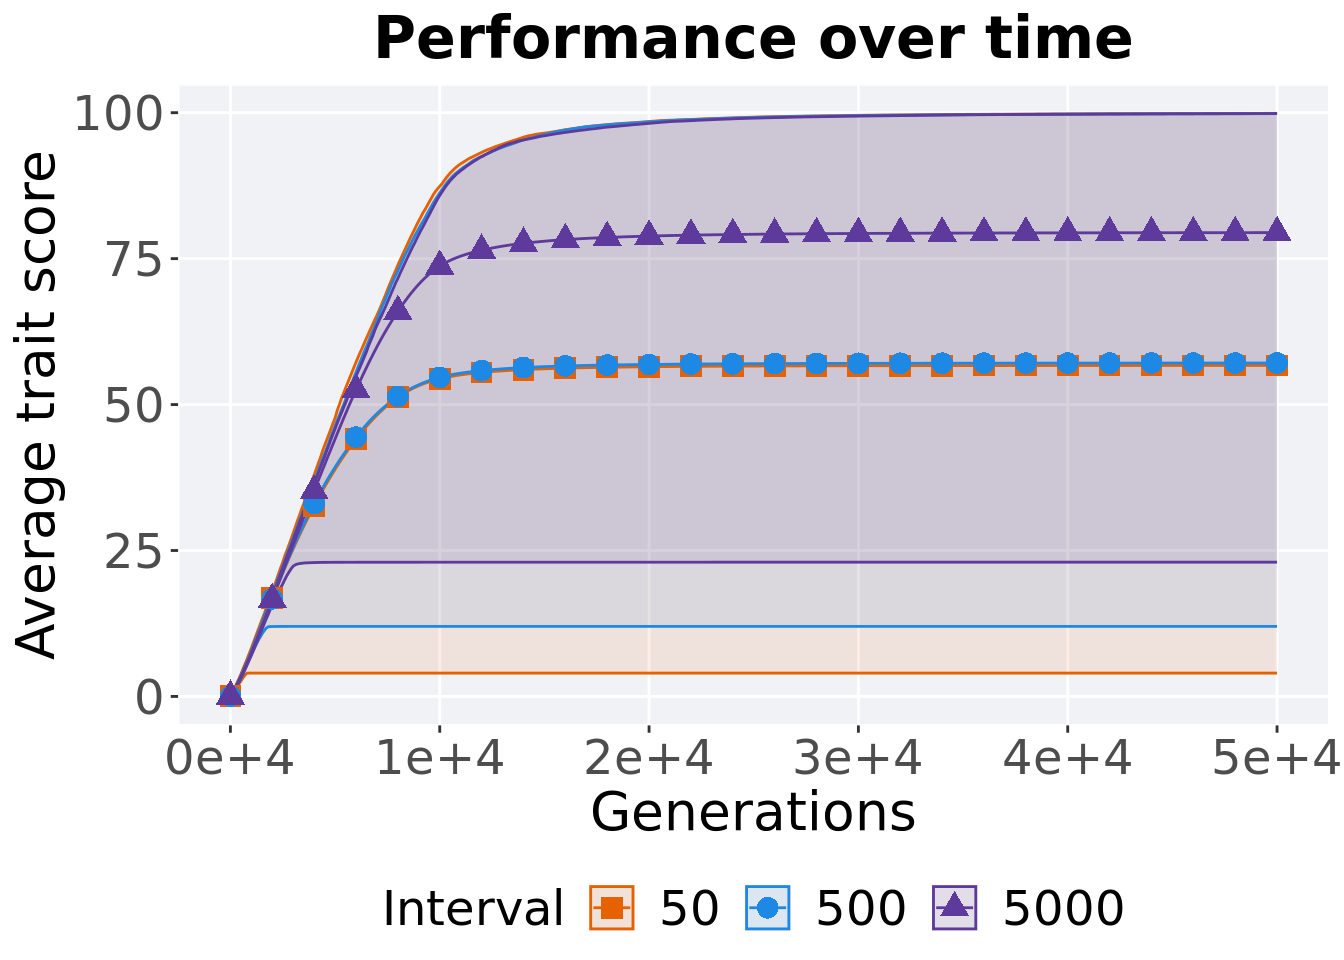
\includegraphics{demo_files/figure-latex/int-tor-mpe-perf-1.pdf}

\hypertarget{best-performance-1}{%
\subsubsection{Best performance}\label{best-performance-1}}

Best performance is found throughout the 50,000 generations.

\begin{Shaded}
\begin{Highlighting}[]
\KeywordTok{filter}\NormalTok{(df_best, Diagnostic }\OperatorTok{==}\StringTok{ 'MULTIPATH_EXPLORATION'} \OperatorTok{&}\StringTok{ `}\DataTypeTok{Selection}\CharTok{\textbackslash{}n}\DataTypeTok{Scheme}\StringTok{`} \OperatorTok{==}\StringTok{ 'TOURNAMENT'} \OperatorTok{&}\StringTok{ }\NormalTok{VAR }\OperatorTok{==}\StringTok{ 'pop_fit_max'}\NormalTok{) }\OperatorTok
\StringTok{  }\KeywordTok{ggplot}\NormalTok{(., }\KeywordTok{aes}\NormalTok{(}\DataTypeTok{x =}\NormalTok{ Interval, }\DataTypeTok{y =}\NormalTok{ VAL }\OperatorTok{/}\StringTok{ }\NormalTok{DIMENSIONALITY, }\DataTypeTok{color =}\NormalTok{ Interval, }\DataTypeTok{fill =}\NormalTok{ Interval, }\DataTypeTok{shape =}\NormalTok{ Interval)) }\OperatorTok{+}
\StringTok{  }\KeywordTok{geom_flat_violin}\NormalTok{(}\DataTypeTok{position =} \KeywordTok{position_nudge}\NormalTok{(}\DataTypeTok{x =} \FloatTok{.2}\NormalTok{, }\DataTypeTok{y =} \DecValTok{0}\NormalTok{), }\DataTypeTok{scale =} \StringTok{'width'}\NormalTok{, }\DataTypeTok{alpha =} \FloatTok{0.2}\NormalTok{) }\OperatorTok{+}
\StringTok{  }\KeywordTok{geom_point}\NormalTok{(}\DataTypeTok{position =} \KeywordTok{position_jitter}\NormalTok{(}\DataTypeTok{width =} \FloatTok{.1}\NormalTok{), }\DataTypeTok{size =} \FloatTok{1.5}\NormalTok{, }\DataTypeTok{alpha =} \FloatTok{1.0}\NormalTok{) }\OperatorTok{+}
\StringTok{  }\KeywordTok{geom_boxplot}\NormalTok{(}\DataTypeTok{color =} \StringTok{'black'}\NormalTok{, }\DataTypeTok{width =} \FloatTok{.2}\NormalTok{, }\DataTypeTok{outlier.shape =} \OtherTok{NA}\NormalTok{, }\DataTypeTok{alpha =} \FloatTok{0.0}\NormalTok{) }\OperatorTok{+}
\StringTok{  }\KeywordTok{scale_y_continuous}\NormalTok{(}
    \DataTypeTok{name=}\StringTok{"Average trait score"}
\NormalTok{  ) }\OperatorTok{+}
\StringTok{  }\KeywordTok{scale_x_discrete}\NormalTok{(}
    \DataTypeTok{name=}\StringTok{"Interval"}
\NormalTok{  )}\OperatorTok{+}
\StringTok{  }\KeywordTok{scale_shape_manual}\NormalTok{(}\DataTypeTok{values=}\NormalTok{SHAPE)}\OperatorTok{+}
\StringTok{  }\KeywordTok{scale_colour_manual}\NormalTok{(}\DataTypeTok{values =}\NormalTok{ cb_palette_mi, ) }\OperatorTok{+}
\StringTok{  }\KeywordTok{scale_fill_manual}\NormalTok{(}\DataTypeTok{values =}\NormalTok{ cb_palette_mi) }\OperatorTok{+}
\StringTok{  }\KeywordTok{ggtitle}\NormalTok{(}\StringTok{'Best performance'}\NormalTok{)}\OperatorTok{+}
\StringTok{  }\NormalTok{p_theme }\OperatorTok{+}\StringTok{ }\KeywordTok{coord_flip}\NormalTok{()}
\end{Highlighting}
\end{Shaded}

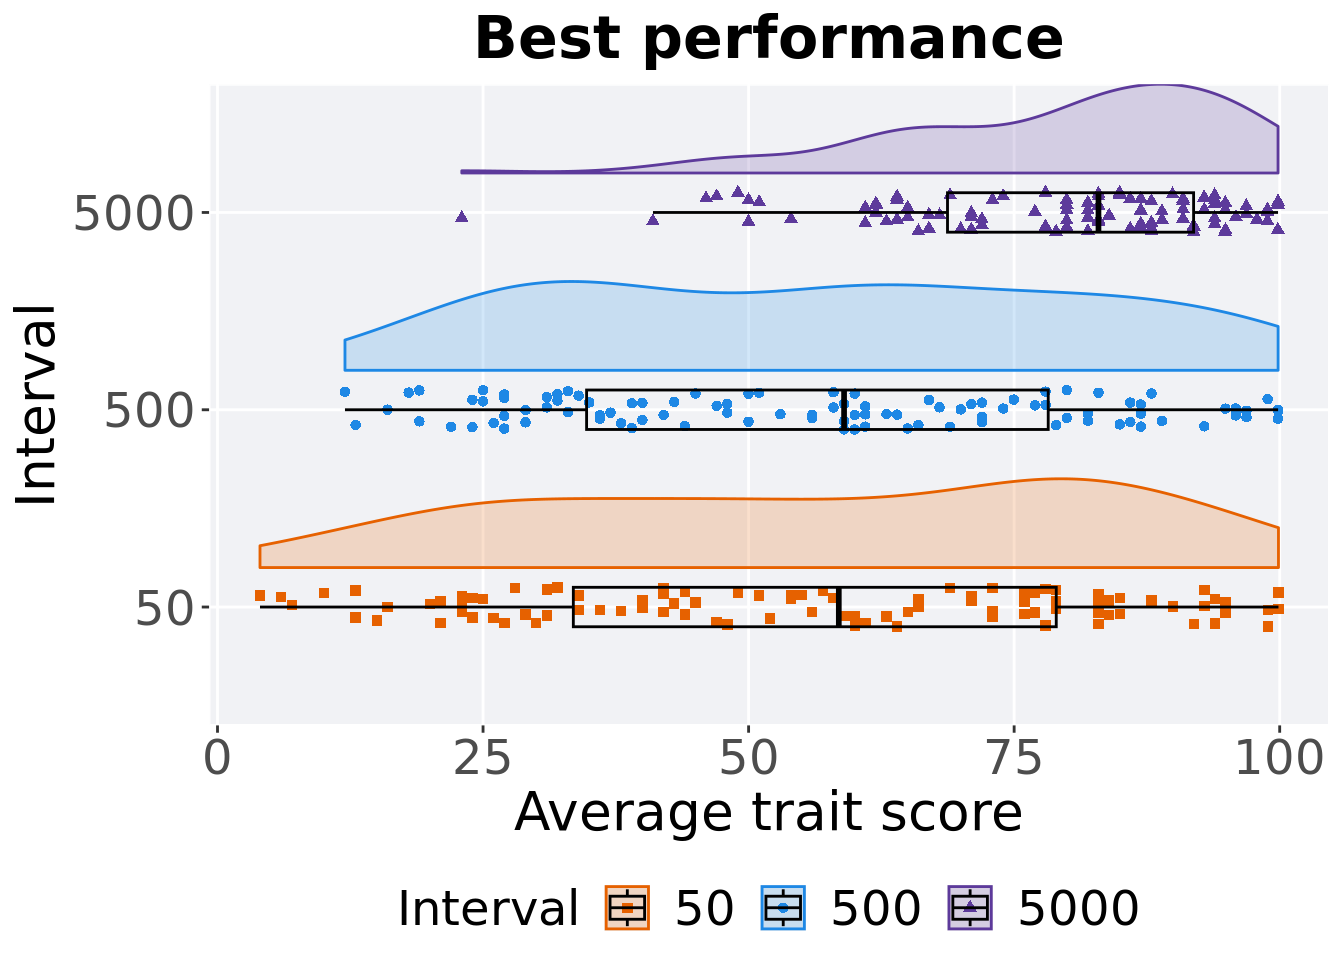
\includegraphics{demo_files/figure-latex/int-tor-mpe-per-bst-1.pdf}

\hypertarget{stats-19}{%
\paragraph{Stats}\label{stats-19}}

Summary statistics for the best performance found.

\begin{Shaded}
\begin{Highlighting}[]
\NormalTok{performance =}\StringTok{ }\KeywordTok{filter}\NormalTok{(df_best, Diagnostic }\OperatorTok{==}\StringTok{ 'MULTIPATH_EXPLORATION'} \OperatorTok{&}\StringTok{ `}\DataTypeTok{Selection}\CharTok{\textbackslash{}n}\DataTypeTok{Scheme}\StringTok{`} \OperatorTok{==}\StringTok{ 'TOURNAMENT'} \OperatorTok{&}\StringTok{ }\NormalTok{VAR }\OperatorTok{==}\StringTok{ 'pop_fit_max'}\NormalTok{)}
\NormalTok{performance }\OperatorTok
\StringTok{  }\KeywordTok{group_by}\NormalTok{(Interval) }\OperatorTok
\StringTok{  }\NormalTok{dplyr}\OperatorTok{::}\KeywordTok{summarise}\NormalTok{(}
    \DataTypeTok{count =} \KeywordTok{n}\NormalTok{(),}
    \DataTypeTok{na_cnt =} \KeywordTok{sum}\NormalTok{(}\KeywordTok{is.na}\NormalTok{(VAL)),}
    \DataTypeTok{min =} \KeywordTok{min}\NormalTok{(VAL, }\DataTypeTok{na.rm =} \OtherTok{TRUE}\NormalTok{) }\OperatorTok{/}\StringTok{ }\NormalTok{DIMENSIONALITY,}
    \DataTypeTok{median =} \KeywordTok{median}\NormalTok{(VAL, }\DataTypeTok{na.rm =} \OtherTok{TRUE}\NormalTok{) }\OperatorTok{/}\StringTok{ }\NormalTok{DIMENSIONALITY,}
    \DataTypeTok{mean =} \KeywordTok{mean}\NormalTok{(VAL, }\DataTypeTok{na.rm =} \OtherTok{TRUE}\NormalTok{) }\OperatorTok{/}\StringTok{ }\NormalTok{DIMENSIONALITY,}
    \DataTypeTok{max =} \KeywordTok{max}\NormalTok{(VAL, }\DataTypeTok{na.rm =} \OtherTok{TRUE}\NormalTok{) }\OperatorTok{/}\StringTok{ }\NormalTok{DIMENSIONALITY,}
    \DataTypeTok{IQR =} \KeywordTok{IQR}\NormalTok{(VAL, }\DataTypeTok{na.rm =} \OtherTok{TRUE}\NormalTok{) }\OperatorTok{/}\StringTok{ }\NormalTok{DIMENSIONALITY}
\NormalTok{  )}
\end{Highlighting}
\end{Shaded}

\begin{verbatim}
## # A tibble: 3 x 8
##   Interval count na_cnt   min median  mean   max   IQR
##   <fct>    <int>  <int> <dbl>  <dbl> <dbl> <dbl> <dbl>
## 1 50         100      0   4     58.5  56.7  99.9  45.5
## 2 500        100      0  12     59.0  57.1  99.9  43.5
## 3 5000       100      0  23.0   82.9  79.5  99.8  23.2
\end{verbatim}

Kruskal--Wallis test provides evidence of difference among selection schemes.

\begin{Shaded}
\begin{Highlighting}[]
\KeywordTok{kruskal.test}\NormalTok{(VAL }\OperatorTok{~}\StringTok{ }\NormalTok{Interval, }\DataTypeTok{data =}\NormalTok{ performance)}
\end{Highlighting}
\end{Shaded}

\begin{verbatim}
## 
##  Kruskal-Wallis rank sum test
## 
## data:  VAL by Interval
## Kruskal-Wallis chi-squared = 50.052, df = 2, p-value = 1.353e-11
\end{verbatim}

Results for post-hoc Wilcoxon rank-sum test with a Bonferroni correction.

\begin{Shaded}
\begin{Highlighting}[]
\KeywordTok{pairwise.wilcox.test}\NormalTok{(}\DataTypeTok{x =}\NormalTok{ performance}\OperatorTok{$}\NormalTok{VAL, }\DataTypeTok{g =}\NormalTok{ performance}\OperatorTok{$}\NormalTok{Interval, }\DataTypeTok{p.adjust.method =} \StringTok{"bonferroni"}\NormalTok{,}
                     \DataTypeTok{paired =} \OtherTok{FALSE}\NormalTok{, }\DataTypeTok{conf.int =} \OtherTok{FALSE}\NormalTok{, }\DataTypeTok{alternative =} \StringTok{'g'}\NormalTok{)}
\end{Highlighting}
\end{Shaded}

\begin{verbatim}
## 
##  Pairwise comparisons using Wilcoxon rank sum test with continuity correction 
## 
## data:  performance$VAL and performance$Interval 
## 
##      50      500    
## 500  1       -      
## 5000 2.6e-09 7.4e-10
## 
## P value adjustment method: bonferroni
\end{verbatim}

\hypertarget{final-performance-1}{%
\subsubsection{Final performance}\label{final-performance-1}}

Best performance is found in final generation.

\begin{Shaded}
\begin{Highlighting}[]
\KeywordTok{filter}\NormalTok{(df_ot, Diagnostic }\OperatorTok{==}\StringTok{ 'MULTIPATH_EXPLORATION'} \OperatorTok{&}\StringTok{ `}\DataTypeTok{Selection}\CharTok{\textbackslash{}n}\DataTypeTok{Scheme}\StringTok{`} \OperatorTok{==}\StringTok{ 'TOURNAMENT'} \OperatorTok{&}\StringTok{ }\NormalTok{Generations }\OperatorTok{==}\StringTok{ }\DecValTok{50000}\NormalTok{) }\OperatorTok
\StringTok{  }\KeywordTok{ggplot}\NormalTok{(., }\KeywordTok{aes}\NormalTok{(}\DataTypeTok{x =}\NormalTok{ Interval, }\DataTypeTok{y =}\NormalTok{ pop_fit_max }\OperatorTok{/}\StringTok{ }\NormalTok{DIMENSIONALITY, }\DataTypeTok{color =}\NormalTok{ Interval, }\DataTypeTok{fill =}\NormalTok{ Interval, }\DataTypeTok{shape =}\NormalTok{ Interval)) }\OperatorTok{+}
\StringTok{  }\KeywordTok{geom_flat_violin}\NormalTok{(}\DataTypeTok{position =} \KeywordTok{position_nudge}\NormalTok{(}\DataTypeTok{x =} \FloatTok{.2}\NormalTok{, }\DataTypeTok{y =} \DecValTok{0}\NormalTok{), }\DataTypeTok{scale =} \StringTok{'width'}\NormalTok{, }\DataTypeTok{alpha =} \FloatTok{0.2}\NormalTok{) }\OperatorTok{+}
\StringTok{  }\KeywordTok{geom_point}\NormalTok{(}\DataTypeTok{position =} \KeywordTok{position_jitter}\NormalTok{(}\DataTypeTok{width =} \FloatTok{.1}\NormalTok{), }\DataTypeTok{size =} \FloatTok{1.5}\NormalTok{, }\DataTypeTok{alpha =} \FloatTok{1.0}\NormalTok{) }\OperatorTok{+}
\StringTok{  }\KeywordTok{geom_boxplot}\NormalTok{(}\DataTypeTok{color =} \StringTok{'black'}\NormalTok{, }\DataTypeTok{width =} \FloatTok{.2}\NormalTok{, }\DataTypeTok{outlier.shape =} \OtherTok{NA}\NormalTok{, }\DataTypeTok{alpha =} \FloatTok{0.0}\NormalTok{) }\OperatorTok{+}
\StringTok{  }\KeywordTok{scale_y_continuous}\NormalTok{(}
    \DataTypeTok{name=}\StringTok{"Average trait score"}
\NormalTok{  ) }\OperatorTok{+}
\StringTok{  }\KeywordTok{scale_x_discrete}\NormalTok{(}
    \DataTypeTok{name=}\StringTok{"Interval"}
\NormalTok{  )}\OperatorTok{+}
\StringTok{  }\KeywordTok{scale_shape_manual}\NormalTok{(}\DataTypeTok{values=}\NormalTok{SHAPE)}\OperatorTok{+}
\StringTok{  }\KeywordTok{scale_colour_manual}\NormalTok{(}\DataTypeTok{values =}\NormalTok{ cb_palette_mi, ) }\OperatorTok{+}
\StringTok{  }\KeywordTok{scale_fill_manual}\NormalTok{(}\DataTypeTok{values =}\NormalTok{ cb_palette_mi) }\OperatorTok{+}
\StringTok{  }\KeywordTok{ggtitle}\NormalTok{(}\StringTok{'Final performance'}\NormalTok{)}\OperatorTok{+}
\StringTok{  }\NormalTok{p_theme }\OperatorTok{+}\StringTok{ }\KeywordTok{coord_flip}\NormalTok{()}
\end{Highlighting}
\end{Shaded}

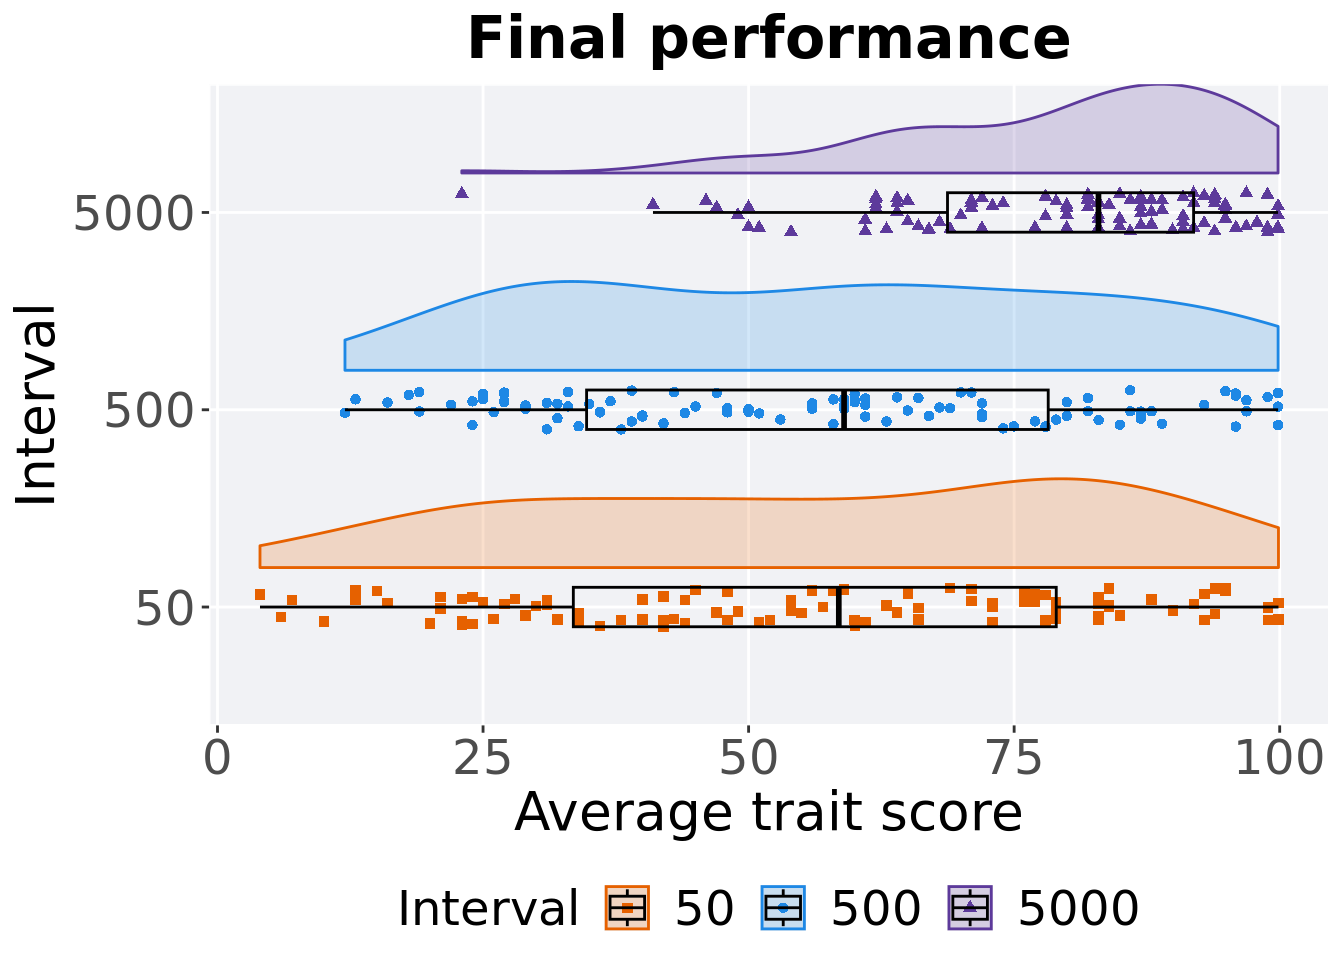
\includegraphics{demo_files/figure-latex/int-tor-mpe-per-end-1.pdf}

\hypertarget{stats-20}{%
\paragraph{Stats}\label{stats-20}}

Summary statistics for best performance is found in final generation.

\begin{Shaded}
\begin{Highlighting}[]
\NormalTok{performance =}\StringTok{ }\KeywordTok{filter}\NormalTok{(df_ot, Diagnostic }\OperatorTok{==}\StringTok{ 'MULTIPATH_EXPLORATION'} \OperatorTok{&}\StringTok{ `}\DataTypeTok{Selection}\CharTok{\textbackslash{}n}\DataTypeTok{Scheme}\StringTok{`} \OperatorTok{==}\StringTok{ 'TOURNAMENT'} \OperatorTok{&}\StringTok{ }\NormalTok{Generations }\OperatorTok{==}\StringTok{ }\DecValTok{50000}\NormalTok{)}
\NormalTok{performance }\OperatorTok
\StringTok{  }\KeywordTok{group_by}\NormalTok{(Interval) }\OperatorTok
\StringTok{  }\NormalTok{dplyr}\OperatorTok{::}\KeywordTok{summarise}\NormalTok{(}
    \DataTypeTok{count =} \KeywordTok{n}\NormalTok{(),}
    \DataTypeTok{na_cnt =} \KeywordTok{sum}\NormalTok{(}\KeywordTok{is.na}\NormalTok{(pop_fit_max)),}
    \DataTypeTok{min =} \KeywordTok{min}\NormalTok{(pop_fit_max }\OperatorTok{/}\StringTok{ }\NormalTok{DIMENSIONALITY, }\DataTypeTok{na.rm =} \OtherTok{TRUE}\NormalTok{),}
    \DataTypeTok{median =} \KeywordTok{median}\NormalTok{(pop_fit_max }\OperatorTok{/}\StringTok{ }\NormalTok{DIMENSIONALITY, }\DataTypeTok{na.rm =} \OtherTok{TRUE}\NormalTok{),}
    \DataTypeTok{mean =} \KeywordTok{mean}\NormalTok{(pop_fit_max }\OperatorTok{/}\StringTok{ }\NormalTok{DIMENSIONALITY, }\DataTypeTok{na.rm =} \OtherTok{TRUE}\NormalTok{),}
    \DataTypeTok{max =} \KeywordTok{max}\NormalTok{(pop_fit_max }\OperatorTok{/}\StringTok{ }\NormalTok{DIMENSIONALITY, }\DataTypeTok{na.rm =} \OtherTok{TRUE}\NormalTok{),}
    \DataTypeTok{IQR =} \KeywordTok{IQR}\NormalTok{(pop_fit_max }\OperatorTok{/}\StringTok{ }\NormalTok{DIMENSIONALITY, }\DataTypeTok{na.rm =} \OtherTok{TRUE}\NormalTok{)}
\NormalTok{  )}
\end{Highlighting}
\end{Shaded}

\begin{verbatim}
## # A tibble: 3 x 8
##   Interval count na_cnt   min median  mean   max   IQR
##   <fct>    <int>  <int> <dbl>  <dbl> <dbl> <dbl> <dbl>
## 1 50         100      0   4     58.5  56.7  99.9  45.5
## 2 500        100      0  12     59.0  57.1  99.9  43.5
## 3 5000       100      0  23.0   82.9  79.5  99.8  23.2
\end{verbatim}

Kruskal--Wallis test provides evidence of difference among selection schemes.

\begin{Shaded}
\begin{Highlighting}[]
\KeywordTok{kruskal.test}\NormalTok{(pop_fit_max }\OperatorTok{~}\StringTok{ }\NormalTok{Interval, }\DataTypeTok{data =}\NormalTok{ performance)}
\end{Highlighting}
\end{Shaded}

\begin{verbatim}
## 
##  Kruskal-Wallis rank sum test
## 
## data:  pop_fit_max by Interval
## Kruskal-Wallis chi-squared = 50.052, df = 2, p-value = 1.353e-11
\end{verbatim}

Results for post-hoc Wilcoxon rank-sum test with a Bonferroni correction.

\begin{Shaded}
\begin{Highlighting}[]
\KeywordTok{pairwise.wilcox.test}\NormalTok{(}\DataTypeTok{x =}\NormalTok{ performance}\OperatorTok{$}\NormalTok{pop_fit_max, }\DataTypeTok{g =}\NormalTok{ performance}\OperatorTok{$}\NormalTok{Interval, }\DataTypeTok{p.adjust.method =} \StringTok{"bonferroni"}\NormalTok{,}
                     \DataTypeTok{paired =} \OtherTok{FALSE}\NormalTok{, }\DataTypeTok{conf.int =} \OtherTok{FALSE}\NormalTok{, }\DataTypeTok{alternative =} \StringTok{'g'}\NormalTok{)}
\end{Highlighting}
\end{Shaded}

\begin{verbatim}
## 
##  Pairwise comparisons using Wilcoxon rank sum test with continuity correction 
## 
## data:  performance$pop_fit_max and performance$Interval 
## 
##      50      500    
## 500  1       -      
## 5000 2.6e-09 7.4e-10
## 
## P value adjustment method: bonferroni
\end{verbatim}

\hypertarget{activation-gene-coverage-4}{%
\subsection{Activation gene coverage}\label{activation-gene-coverage-4}}

Activation gene coverage analysis.

\hypertarget{coverage-over-time-7}{%
\subsubsection{Coverage over time}\label{coverage-over-time-7}}

Activation gene coverage over time.

\begin{Shaded}
\begin{Highlighting}[]
\CommentTok{# data for lines and shading on plots}
\NormalTok{lines =}\StringTok{ }\KeywordTok{filter}\NormalTok{(df_ot, Diagnostic }\OperatorTok{==}\StringTok{ 'MULTIPATH_EXPLORATION'} \OperatorTok{&}\StringTok{ `}\DataTypeTok{Selection}\CharTok{\textbackslash{}n}\DataTypeTok{Scheme}\StringTok{`} \OperatorTok{==}\StringTok{ 'TOURNAMENT'}\NormalTok{) }\OperatorTok
\StringTok{  }\KeywordTok{group_by}\NormalTok{(Interval, Generations) }\OperatorTok
\StringTok{  }\NormalTok{dplyr}\OperatorTok{::}\KeywordTok{summarise}\NormalTok{(}
    \DataTypeTok{min =} \KeywordTok{min}\NormalTok{(pop_act_cov),}
    \DataTypeTok{mean =} \KeywordTok{mean}\NormalTok{(pop_act_cov),}
    \DataTypeTok{max =} \KeywordTok{max}\NormalTok{(pop_act_cov)}
\NormalTok{  )}
\end{Highlighting}
\end{Shaded}

\begin{verbatim}
## `summarise()` has grouped output by 'Interval'. You can override using the
## `.groups` argument.
\end{verbatim}

\begin{Shaded}
\begin{Highlighting}[]
\KeywordTok{ggplot}\NormalTok{(lines, }\KeywordTok{aes}\NormalTok{(}\DataTypeTok{x=}\NormalTok{Generations, }\DataTypeTok{y=}\NormalTok{mean, }\DataTypeTok{group =}\NormalTok{ Interval, }\DataTypeTok{fill =}\NormalTok{ Interval, }\DataTypeTok{color =}\NormalTok{ Interval, }\DataTypeTok{shape =}\NormalTok{ Interval)) }\OperatorTok{+}
\StringTok{  }\KeywordTok{geom_ribbon}\NormalTok{(}\KeywordTok{aes}\NormalTok{(}\DataTypeTok{ymin =}\NormalTok{ min, }\DataTypeTok{ymax =}\NormalTok{ max), }\DataTypeTok{alpha =} \FloatTok{0.1}\NormalTok{) }\OperatorTok{+}
\StringTok{  }\KeywordTok{geom_line}\NormalTok{(}\DataTypeTok{size =} \FloatTok{0.5}\NormalTok{) }\OperatorTok{+}
\StringTok{  }\KeywordTok{geom_point}\NormalTok{(}\DataTypeTok{data =} \KeywordTok{filter}\NormalTok{(lines, Generations }\OperatorTok\StringTok{ }\DecValTok{2000} \OperatorTok{==}\StringTok{ }\DecValTok{0}\NormalTok{), }\DataTypeTok{size =} \FloatTok{1.5}\NormalTok{, }\DataTypeTok{stroke =} \FloatTok{2.0}\NormalTok{, }\DataTypeTok{alpha =} \FloatTok{1.0}\NormalTok{) }\OperatorTok{+}
\StringTok{  }\KeywordTok{scale_y_continuous}\NormalTok{(}
    \DataTypeTok{name=}\StringTok{"Coverage"}
\NormalTok{  ) }\OperatorTok{+}
\StringTok{  }\KeywordTok{scale_x_continuous}\NormalTok{(}
    \DataTypeTok{name=}\StringTok{"Generations"}\NormalTok{,}
    \DataTypeTok{limits=}\KeywordTok{c}\NormalTok{(}\DecValTok{0}\NormalTok{, }\DecValTok{50000}\NormalTok{),}
    \DataTypeTok{breaks=}\KeywordTok{c}\NormalTok{(}\DecValTok{0}\NormalTok{, }\DecValTok{10000}\NormalTok{, }\DecValTok{20000}\NormalTok{, }\DecValTok{30000}\NormalTok{, }\DecValTok{40000}\NormalTok{, }\DecValTok{50000}\NormalTok{),}
    \DataTypeTok{labels=}\KeywordTok{c}\NormalTok{(}\StringTok{"0e+4"}\NormalTok{, }\StringTok{"1e+4"}\NormalTok{, }\StringTok{"2e+4"}\NormalTok{, }\StringTok{"3e+4"}\NormalTok{, }\StringTok{"4e+4"}\NormalTok{, }\StringTok{"5e+4"}\NormalTok{)}

\NormalTok{  ) }\OperatorTok{+}
\StringTok{  }\KeywordTok{scale_shape_manual}\NormalTok{(}\DataTypeTok{values=}\NormalTok{SHAPE)}\OperatorTok{+}
\StringTok{  }\KeywordTok{scale_colour_manual}\NormalTok{(}\DataTypeTok{values =}\NormalTok{ cb_palette_mi) }\OperatorTok{+}
\StringTok{  }\KeywordTok{scale_fill_manual}\NormalTok{(}\DataTypeTok{values =}\NormalTok{ cb_palette_mi) }\OperatorTok{+}
\StringTok{  }\KeywordTok{ggtitle}\NormalTok{(}\StringTok{'Activation gene coverage over time'}\NormalTok{)}\OperatorTok{+}
\StringTok{  }\NormalTok{p_theme}
\end{Highlighting}
\end{Shaded}

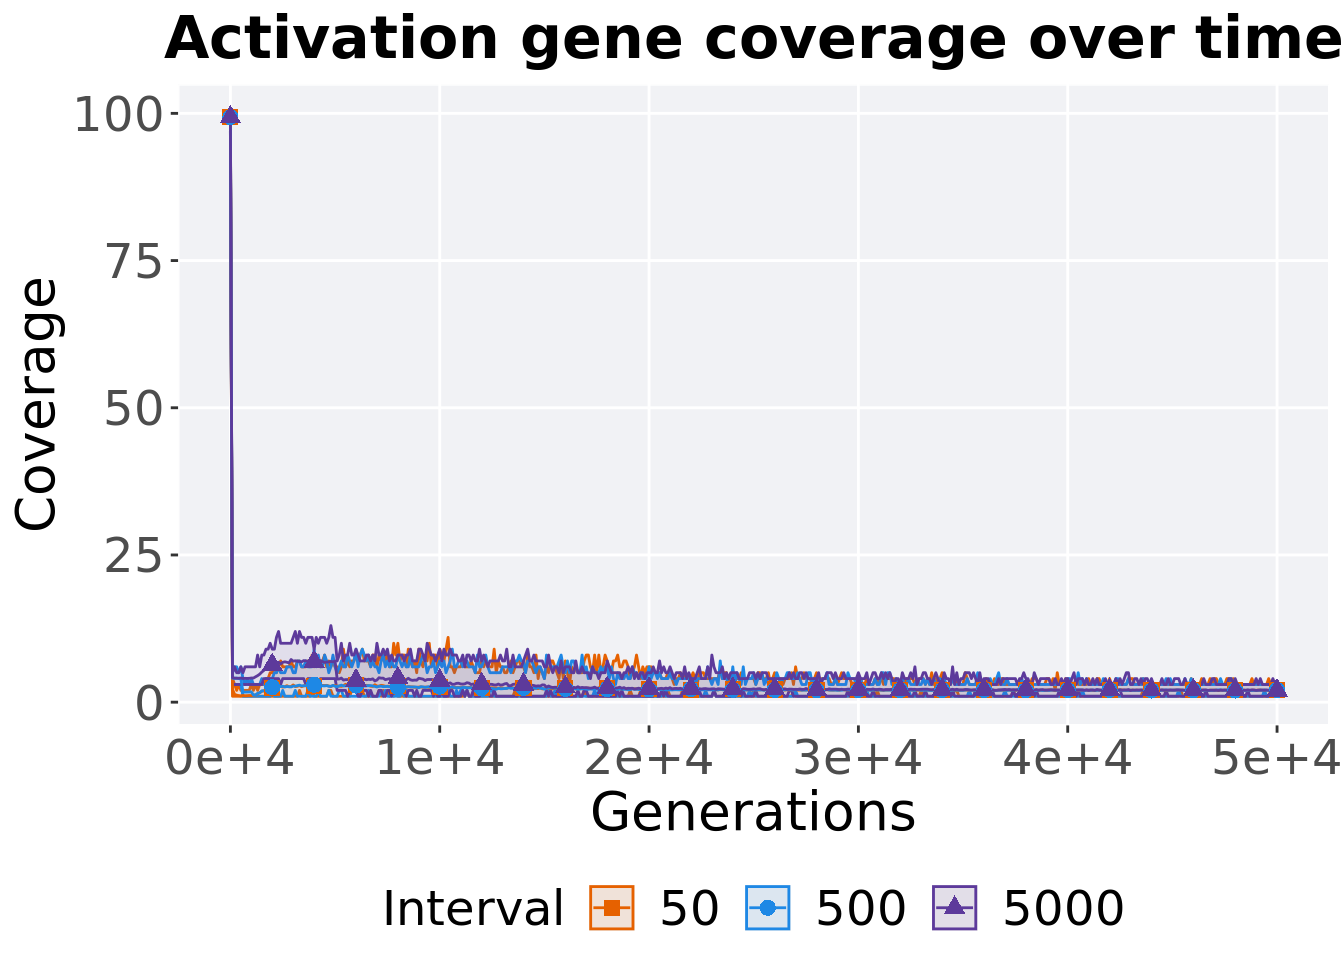
\includegraphics{demo_files/figure-latex/int-mpe-act-tor-ot-1.pdf}

\hypertarget{end-of-50000-generations-7}{%
\subsubsection{End of 50,000 generations}\label{end-of-50000-generations-7}}

Activation gene coverage in the population at the end of 50,000 generations.

\begin{Shaded}
\begin{Highlighting}[]
\CommentTok{### end of run}
\KeywordTok{filter}\NormalTok{(df_ot, Diagnostic }\OperatorTok{==}\StringTok{ 'MULTIPATH_EXPLORATION'} \OperatorTok{&}\StringTok{ `}\DataTypeTok{Selection}\CharTok{\textbackslash{}n}\DataTypeTok{Scheme}\StringTok{`} \OperatorTok{==}\StringTok{ 'TOURNAMENT'} \OperatorTok{&}\StringTok{ }\NormalTok{Generations }\OperatorTok{==}\StringTok{ }\DecValTok{50000}\NormalTok{) }\OperatorTok
\StringTok{  }\KeywordTok{ggplot}\NormalTok{(., }\KeywordTok{aes}\NormalTok{(}\DataTypeTok{x =}\NormalTok{ Interval, }\DataTypeTok{y =}\NormalTok{ pop_act_cov, }\DataTypeTok{color =}\NormalTok{ Interval, }\DataTypeTok{fill =}\NormalTok{ Interval, }\DataTypeTok{shape =}\NormalTok{ Interval)) }\OperatorTok{+}
\StringTok{  }\KeywordTok{geom_flat_violin}\NormalTok{(}\DataTypeTok{position =} \KeywordTok{position_nudge}\NormalTok{(}\DataTypeTok{x =} \FloatTok{.2}\NormalTok{, }\DataTypeTok{y =} \DecValTok{0}\NormalTok{), }\DataTypeTok{scale =} \StringTok{'width'}\NormalTok{, }\DataTypeTok{alpha =} \FloatTok{0.3}\NormalTok{) }\OperatorTok{+}
\StringTok{  }\KeywordTok{geom_point}\NormalTok{(}\DataTypeTok{position =} \KeywordTok{position_jitter}\NormalTok{(}\DataTypeTok{height =} \FloatTok{.05}\NormalTok{, }\DataTypeTok{width =} \FloatTok{.05}\NormalTok{), }\DataTypeTok{size =} \FloatTok{1.5}\NormalTok{, }\DataTypeTok{alpha =} \FloatTok{0.5}\NormalTok{) }\OperatorTok{+}
\StringTok{  }\KeywordTok{geom_boxplot}\NormalTok{(}\DataTypeTok{color =} \StringTok{'black'}\NormalTok{, }\DataTypeTok{width =} \FloatTok{.2}\NormalTok{, }\DataTypeTok{outlier.shape =} \OtherTok{NA}\NormalTok{, }\DataTypeTok{alpha =} \FloatTok{0.0}\NormalTok{) }\OperatorTok{+}
\StringTok{  }\KeywordTok{scale_shape_manual}\NormalTok{(}\DataTypeTok{values=}\NormalTok{SHAPE)}\OperatorTok{+}
\StringTok{  }\KeywordTok{scale_y_continuous}\NormalTok{(}
    \DataTypeTok{name=}\StringTok{"Coverage"}
\NormalTok{  ) }\OperatorTok{+}
\StringTok{  }\KeywordTok{scale_x_discrete}\NormalTok{(}
    \DataTypeTok{name=}\StringTok{"Interval"}
\NormalTok{  ) }\OperatorTok{+}
\StringTok{  }\KeywordTok{scale_colour_manual}\NormalTok{(}\DataTypeTok{values =}\NormalTok{ cb_palette_mi) }\OperatorTok{+}
\StringTok{  }\KeywordTok{scale_fill_manual}\NormalTok{(}\DataTypeTok{values =}\NormalTok{ cb_palette_mi) }\OperatorTok{+}
\StringTok{  }\KeywordTok{ggtitle}\NormalTok{(}\StringTok{'Final activation gene coverage'}\NormalTok{)}\OperatorTok{+}
\StringTok{  }\NormalTok{p_theme }\OperatorTok{+}\StringTok{ }\KeywordTok{coord_flip}\NormalTok{()}
\end{Highlighting}
\end{Shaded}

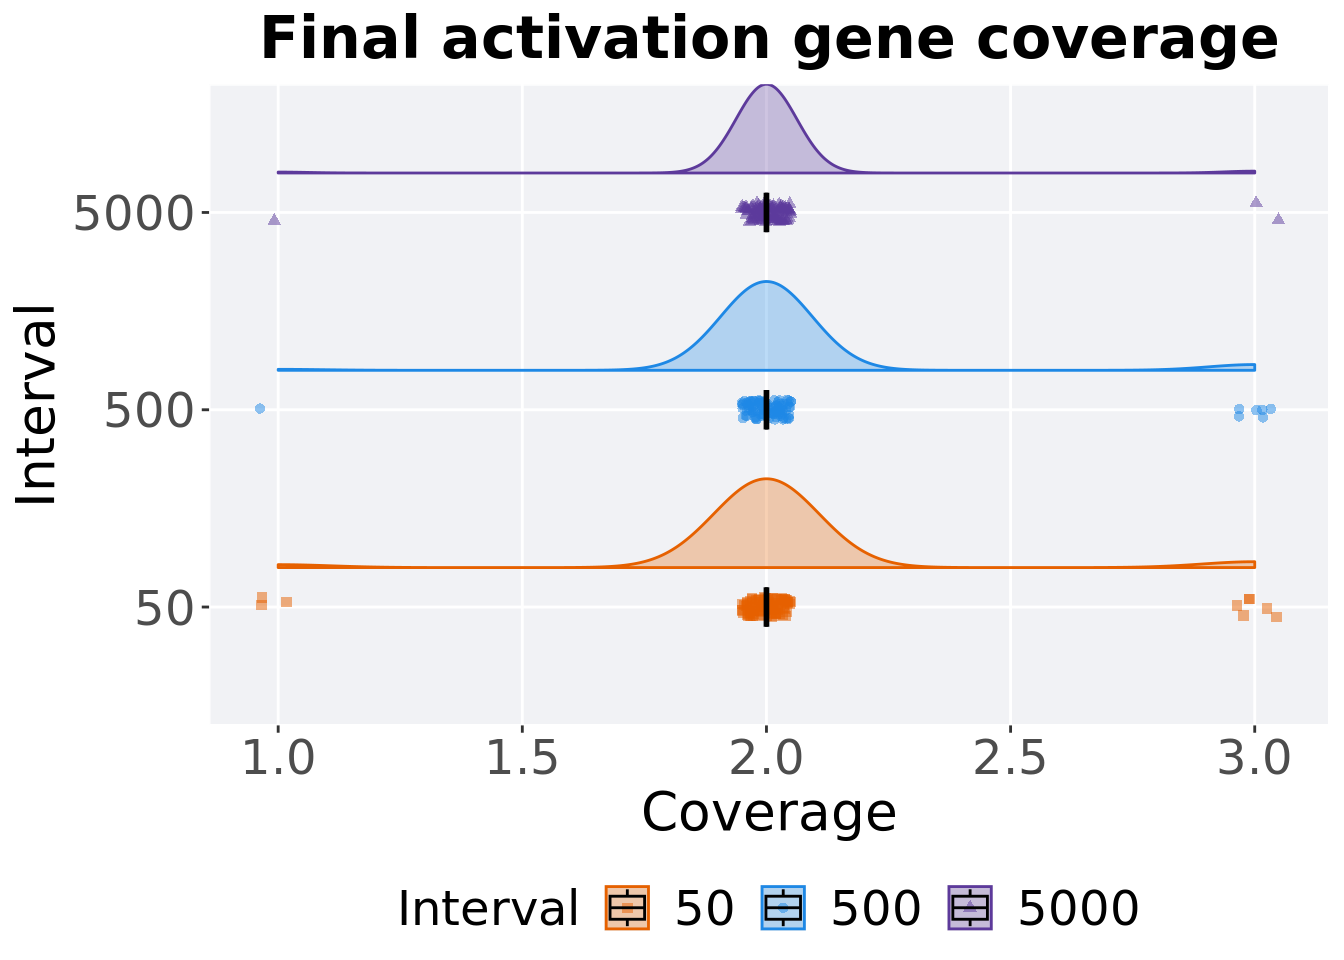
\includegraphics{demo_files/figure-latex/int-mpe-act-tor-end-1.pdf}

\hypertarget{stats-21}{%
\paragraph{Stats}\label{stats-21}}

Summary statistics for activation gene coverage.

\begin{Shaded}
\begin{Highlighting}[]
\NormalTok{coverage =}\StringTok{ }\KeywordTok{filter}\NormalTok{(df_ot, Diagnostic }\OperatorTok{==}\StringTok{ 'MULTIPATH_EXPLORATION'} \OperatorTok{&}\StringTok{ `}\DataTypeTok{Selection}\CharTok{\textbackslash{}n}\DataTypeTok{Scheme}\StringTok{`} \OperatorTok{==}\StringTok{ 'TOURNAMENT'} \OperatorTok{&}\StringTok{ }\NormalTok{Generations }\OperatorTok{==}\StringTok{ }\DecValTok{50000}\NormalTok{)}
\NormalTok{coverage }\OperatorTok
\StringTok{  }\KeywordTok{group_by}\NormalTok{(Interval) }\OperatorTok
\StringTok{  }\NormalTok{dplyr}\OperatorTok{::}\KeywordTok{summarise}\NormalTok{(}
    \DataTypeTok{count =} \KeywordTok{n}\NormalTok{(),}
    \DataTypeTok{na_cnt =} \KeywordTok{sum}\NormalTok{(}\KeywordTok{is.na}\NormalTok{(pop_act_cov)),}
    \DataTypeTok{min =} \KeywordTok{min}\NormalTok{(pop_act_cov, }\DataTypeTok{na.rm =} \OtherTok{TRUE}\NormalTok{),}
    \DataTypeTok{median =} \KeywordTok{median}\NormalTok{(pop_act_cov, }\DataTypeTok{na.rm =} \OtherTok{TRUE}\NormalTok{),}
    \DataTypeTok{mean =} \KeywordTok{mean}\NormalTok{(pop_act_cov, }\DataTypeTok{na.rm =} \OtherTok{TRUE}\NormalTok{),}
    \DataTypeTok{max =} \KeywordTok{max}\NormalTok{(pop_act_cov, }\DataTypeTok{na.rm =} \OtherTok{TRUE}\NormalTok{),}
    \DataTypeTok{IQR =} \KeywordTok{IQR}\NormalTok{(pop_act_cov, }\DataTypeTok{na.rm =} \OtherTok{TRUE}\NormalTok{)}
\NormalTok{  )}
\end{Highlighting}
\end{Shaded}

\begin{verbatim}
## # A tibble: 3 x 8
##   Interval count na_cnt   min median  mean   max   IQR
##   <fct>    <int>  <int> <int>  <dbl> <dbl> <int> <dbl>
## 1 50         100      0     1      2  2.03     3     0
## 2 500        100      0     1      2  2.05     3     0
## 3 5000       100      0     1      2  2.01     3     0
\end{verbatim}

Kruskal--Wallis test provides evidence of no difference among activation gene coverage.

\begin{Shaded}
\begin{Highlighting}[]
\KeywordTok{kruskal.test}\NormalTok{(pop_act_cov }\OperatorTok{~}\StringTok{ }\NormalTok{Interval, }\DataTypeTok{data =}\NormalTok{ coverage)}
\end{Highlighting}
\end{Shaded}

\begin{verbatim}
## 
##  Kruskal-Wallis rank sum test
## 
## data:  pop_act_cov by Interval
## Kruskal-Wallis chi-squared = 1.299, df = 2, p-value = 0.5223
\end{verbatim}

\hypertarget{lexicase-selection-3}{%
\section{Lexicase selection}\label{lexicase-selection-3}}

Here we analyze how the different population structures affect standard lexicase selection on the contradictory objectives diagnostic.

\hypertarget{performance-2}{%
\subsection{Performance}\label{performance-2}}

\hypertarget{performance-over-time-8}{%
\subsubsection{Performance over time}\label{performance-over-time-8}}

\begin{Shaded}
\begin{Highlighting}[]
\NormalTok{lines =}\StringTok{ }\KeywordTok{filter}\NormalTok{(df_ot, Diagnostic }\OperatorTok{==}\StringTok{ 'MULTIPATH_EXPLORATION'} \OperatorTok{&}\StringTok{ `}\DataTypeTok{Selection}\CharTok{\textbackslash{}n}\DataTypeTok{Scheme}\StringTok{`} \OperatorTok{==}\StringTok{ 'LEXICASE'}\NormalTok{) }\OperatorTok
\StringTok{  }\KeywordTok{group_by}\NormalTok{(Interval, Generations) }\OperatorTok
\StringTok{  }\NormalTok{dplyr}\OperatorTok{::}\KeywordTok{summarise}\NormalTok{(}
    \DataTypeTok{min =} \KeywordTok{min}\NormalTok{(pop_fit_max) }\OperatorTok{/}\StringTok{ }\NormalTok{DIMENSIONALITY,}
    \DataTypeTok{mean =} \KeywordTok{mean}\NormalTok{(pop_fit_max) }\OperatorTok{/}\StringTok{ }\NormalTok{DIMENSIONALITY,}
    \DataTypeTok{max =} \KeywordTok{max}\NormalTok{(pop_fit_max) }\OperatorTok{/}\StringTok{ }\NormalTok{DIMENSIONALITY}
\NormalTok{  )}
\KeywordTok{ggplot}\NormalTok{(lines, }\KeywordTok{aes}\NormalTok{(}\DataTypeTok{x=}\NormalTok{Generations, }\DataTypeTok{y=}\NormalTok{mean, }\DataTypeTok{group =}\NormalTok{ Interval, }\DataTypeTok{fill =}\NormalTok{ Interval, }\DataTypeTok{color =}\NormalTok{ Interval, }\DataTypeTok{shape =}\NormalTok{ Interval)) }\OperatorTok{+}
\StringTok{  }\KeywordTok{geom_ribbon}\NormalTok{(}\KeywordTok{aes}\NormalTok{(}\DataTypeTok{ymin =}\NormalTok{ min, }\DataTypeTok{ymax =}\NormalTok{ max), }\DataTypeTok{alpha =} \FloatTok{0.1}\NormalTok{) }\OperatorTok{+}
\StringTok{  }\KeywordTok{geom_line}\NormalTok{(}\DataTypeTok{size =} \FloatTok{0.5}\NormalTok{) }\OperatorTok{+}
\StringTok{  }\KeywordTok{geom_point}\NormalTok{(}\DataTypeTok{data =} \KeywordTok{filter}\NormalTok{(lines, Generations }\OperatorTok\StringTok{ }\DecValTok{2000} \OperatorTok{==}\StringTok{ }\DecValTok{0}\NormalTok{), }\DataTypeTok{size =} \FloatTok{2.5}\NormalTok{, }\DataTypeTok{stroke =} \FloatTok{2.0}\NormalTok{, }\DataTypeTok{alpha =} \FloatTok{1.0}\NormalTok{) }\OperatorTok{+}
\StringTok{  }\KeywordTok{scale_y_continuous}\NormalTok{(}
    \DataTypeTok{name=}\StringTok{"Average trait score"}
\NormalTok{  ) }\OperatorTok{+}
\StringTok{  }\KeywordTok{scale_x_continuous}\NormalTok{(}
    \DataTypeTok{name=}\StringTok{"Generations"}\NormalTok{,}
    \DataTypeTok{limits=}\KeywordTok{c}\NormalTok{(}\DecValTok{0}\NormalTok{, }\DecValTok{50000}\NormalTok{),}
    \DataTypeTok{breaks=}\KeywordTok{c}\NormalTok{(}\DecValTok{0}\NormalTok{, }\DecValTok{10000}\NormalTok{, }\DecValTok{20000}\NormalTok{, }\DecValTok{30000}\NormalTok{, }\DecValTok{40000}\NormalTok{, }\DecValTok{50000}\NormalTok{),}
    \DataTypeTok{labels=}\KeywordTok{c}\NormalTok{(}\StringTok{"0e+4"}\NormalTok{, }\StringTok{"1e+4"}\NormalTok{, }\StringTok{"2e+4"}\NormalTok{, }\StringTok{"3e+4"}\NormalTok{, }\StringTok{"4e+4"}\NormalTok{, }\StringTok{"5e+4"}\NormalTok{)}

\NormalTok{  ) }\OperatorTok{+}
\StringTok{  }\KeywordTok{scale_shape_manual}\NormalTok{(}\DataTypeTok{values=}\NormalTok{SHAPE)}\OperatorTok{+}
\StringTok{  }\KeywordTok{scale_colour_manual}\NormalTok{(}\DataTypeTok{values =}\NormalTok{ cb_palette_mi) }\OperatorTok{+}
\StringTok{  }\KeywordTok{scale_fill_manual}\NormalTok{(}\DataTypeTok{values =}\NormalTok{ cb_palette_mi) }\OperatorTok{+}
\StringTok{  }\KeywordTok{ggtitle}\NormalTok{(}\StringTok{"Performance over time"}\NormalTok{) }\OperatorTok{+}
\StringTok{  }\NormalTok{p_theme}
\end{Highlighting}
\end{Shaded}

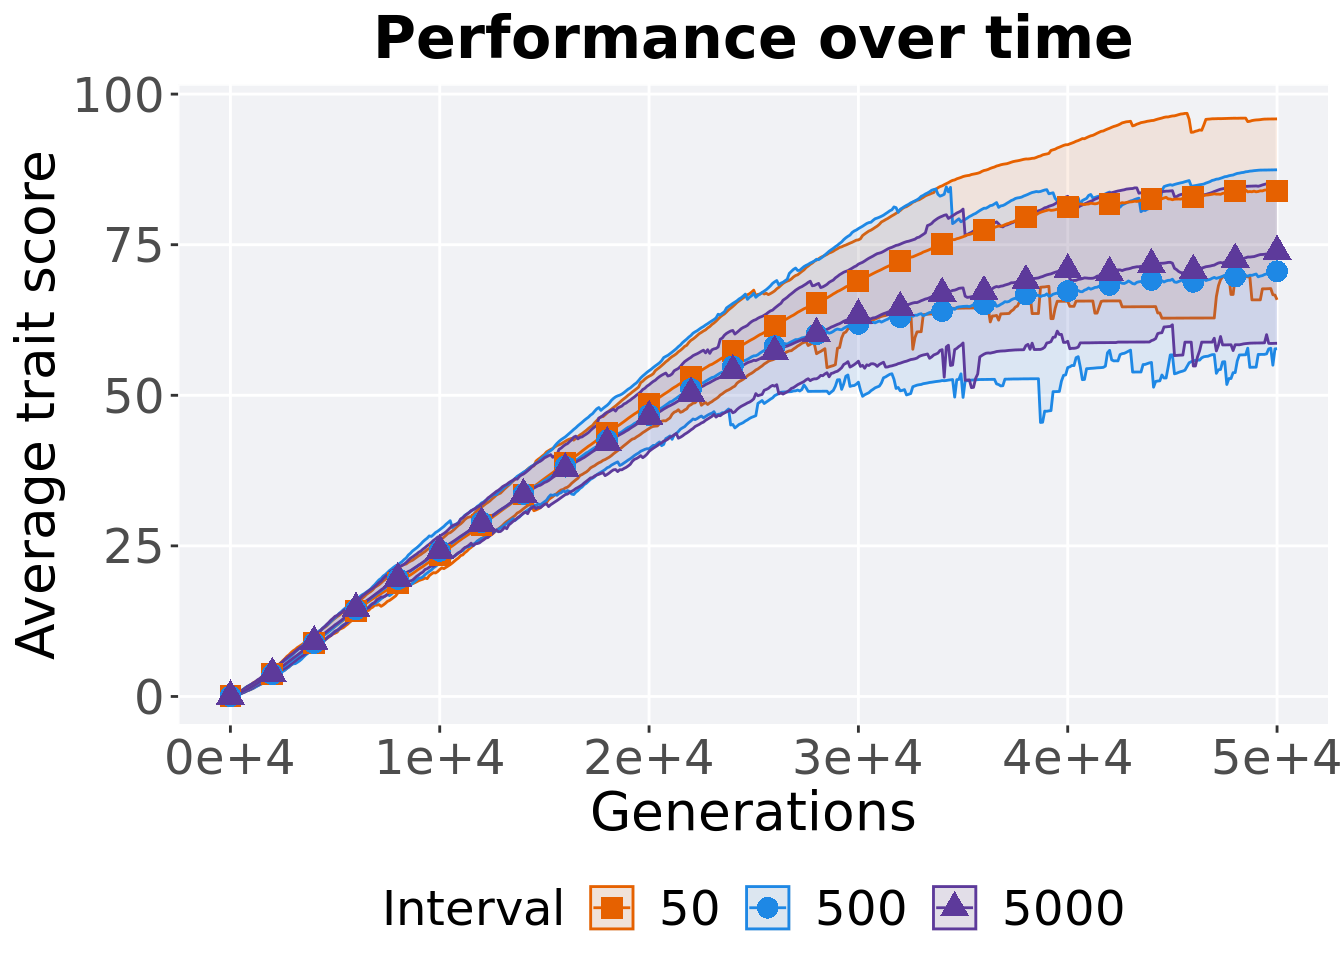
\includegraphics{demo_files/figure-latex/int-lex-mpe-perf-1.pdf}

\hypertarget{best-performance-2}{%
\subsubsection{Best performance}\label{best-performance-2}}

Best performance is found throughout in final generation.

\begin{Shaded}
\begin{Highlighting}[]
\KeywordTok{filter}\NormalTok{(df_best, Diagnostic }\OperatorTok{==}\StringTok{ 'MULTIPATH_EXPLORATION'} \OperatorTok{&}\StringTok{ `}\DataTypeTok{Selection}\CharTok{\textbackslash{}n}\DataTypeTok{Scheme}\StringTok{`} \OperatorTok{==}\StringTok{ 'LEXICASE'} \OperatorTok{&}\StringTok{ }\NormalTok{VAR }\OperatorTok{==}\StringTok{ 'pop_fit_max'}\NormalTok{) }\OperatorTok
\StringTok{  }\KeywordTok{ggplot}\NormalTok{(., }\KeywordTok{aes}\NormalTok{(}\DataTypeTok{x =}\NormalTok{ Interval, }\DataTypeTok{y =}\NormalTok{ VAL }\OperatorTok{/}\StringTok{ }\NormalTok{DIMENSIONALITY, }\DataTypeTok{color =}\NormalTok{ Interval, }\DataTypeTok{fill =}\NormalTok{ Interval, }\DataTypeTok{shape =}\NormalTok{ Interval)) }\OperatorTok{+}
\StringTok{  }\KeywordTok{geom_flat_violin}\NormalTok{(}\DataTypeTok{position =} \KeywordTok{position_nudge}\NormalTok{(}\DataTypeTok{x =} \FloatTok{.2}\NormalTok{, }\DataTypeTok{y =} \DecValTok{0}\NormalTok{), }\DataTypeTok{scale =} \StringTok{'width'}\NormalTok{, }\DataTypeTok{alpha =} \FloatTok{0.2}\NormalTok{) }\OperatorTok{+}
\StringTok{  }\KeywordTok{geom_point}\NormalTok{(}\DataTypeTok{position =} \KeywordTok{position_jitter}\NormalTok{(}\DataTypeTok{width =} \FloatTok{.1}\NormalTok{), }\DataTypeTok{size =} \FloatTok{1.5}\NormalTok{, }\DataTypeTok{alpha =} \FloatTok{1.0}\NormalTok{) }\OperatorTok{+}
\StringTok{  }\KeywordTok{geom_boxplot}\NormalTok{(}\DataTypeTok{color =} \StringTok{'black'}\NormalTok{, }\DataTypeTok{width =} \FloatTok{.2}\NormalTok{, }\DataTypeTok{outlier.shape =} \OtherTok{NA}\NormalTok{, }\DataTypeTok{alpha =} \FloatTok{0.0}\NormalTok{) }\OperatorTok{+}
\StringTok{  }\KeywordTok{scale_y_continuous}\NormalTok{(}
    \DataTypeTok{name=}\StringTok{"Average trait score"}
\NormalTok{  ) }\OperatorTok{+}
\StringTok{  }\KeywordTok{scale_x_discrete}\NormalTok{(}
    \DataTypeTok{name=}\StringTok{"Interval"}
\NormalTok{  )}\OperatorTok{+}
\StringTok{  }\KeywordTok{scale_shape_manual}\NormalTok{(}\DataTypeTok{values=}\NormalTok{SHAPE)}\OperatorTok{+}
\StringTok{  }\KeywordTok{scale_colour_manual}\NormalTok{(}\DataTypeTok{values =}\NormalTok{ cb_palette_mi, ) }\OperatorTok{+}
\StringTok{  }\KeywordTok{scale_fill_manual}\NormalTok{(}\DataTypeTok{values =}\NormalTok{ cb_palette_mi) }\OperatorTok{+}
\StringTok{  }\KeywordTok{ggtitle}\NormalTok{(}\StringTok{'Best performance'}\NormalTok{)}\OperatorTok{+}
\StringTok{  }\NormalTok{p_theme }\OperatorTok{+}\StringTok{ }\KeywordTok{coord_flip}\NormalTok{()}
\end{Highlighting}
\end{Shaded}

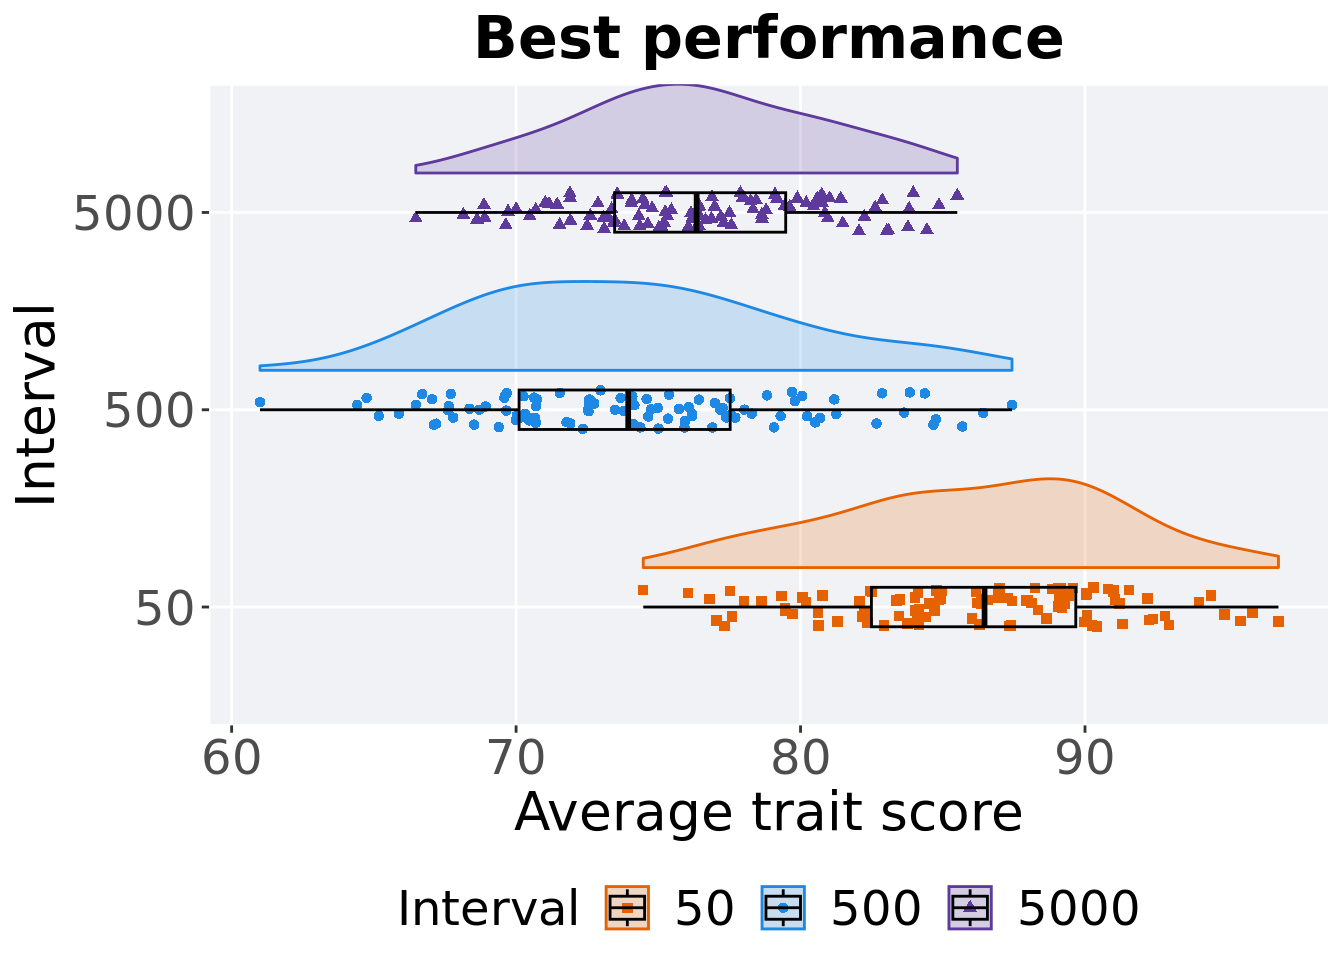
\includegraphics{demo_files/figure-latex/int-lex-mpe-per-bst-1.pdf}

\hypertarget{stats-22}{%
\paragraph{Stats}\label{stats-22}}

Summary statistics for the best performance found.

\begin{Shaded}
\begin{Highlighting}[]
\NormalTok{performance =}\StringTok{ }\KeywordTok{filter}\NormalTok{(df_best, Diagnostic }\OperatorTok{==}\StringTok{ 'MULTIPATH_EXPLORATION'} \OperatorTok{&}\StringTok{ `}\DataTypeTok{Selection}\CharTok{\textbackslash{}n}\DataTypeTok{Scheme}\StringTok{`} \OperatorTok{==}\StringTok{ 'LEXICASE'} \OperatorTok{&}\StringTok{ }\NormalTok{VAR }\OperatorTok{==}\StringTok{ 'pop_fit_max'}\NormalTok{)}
\NormalTok{performance}\OperatorTok{$}\NormalTok{Interval =}\StringTok{ }\KeywordTok{factor}\NormalTok{(performance}\OperatorTok{$}\NormalTok{Interval, }\DataTypeTok{levels =} \KeywordTok{c}\NormalTok{(}\StringTok{'50'}\NormalTok{,}\StringTok{'5000'}\NormalTok{,}\StringTok{'500'}\NormalTok{))}
\NormalTok{performance }\OperatorTok
\StringTok{  }\KeywordTok{group_by}\NormalTok{(Interval) }\OperatorTok
\StringTok{  }\NormalTok{dplyr}\OperatorTok{::}\KeywordTok{summarise}\NormalTok{(}
    \DataTypeTok{count =} \KeywordTok{n}\NormalTok{(),}
    \DataTypeTok{na_cnt =} \KeywordTok{sum}\NormalTok{(}\KeywordTok{is.na}\NormalTok{(VAL)),}
    \DataTypeTok{min =} \KeywordTok{min}\NormalTok{(VAL, }\DataTypeTok{na.rm =} \OtherTok{TRUE}\NormalTok{) }\OperatorTok{/}\StringTok{ }\NormalTok{DIMENSIONALITY,}
    \DataTypeTok{median =} \KeywordTok{median}\NormalTok{(VAL, }\DataTypeTok{na.rm =} \OtherTok{TRUE}\NormalTok{) }\OperatorTok{/}\StringTok{ }\NormalTok{DIMENSIONALITY,}
    \DataTypeTok{mean =} \KeywordTok{mean}\NormalTok{(VAL, }\DataTypeTok{na.rm =} \OtherTok{TRUE}\NormalTok{) }\OperatorTok{/}\StringTok{ }\NormalTok{DIMENSIONALITY,}
    \DataTypeTok{max =} \KeywordTok{max}\NormalTok{(VAL, }\DataTypeTok{na.rm =} \OtherTok{TRUE}\NormalTok{) }\OperatorTok{/}\StringTok{ }\NormalTok{DIMENSIONALITY,}
    \DataTypeTok{IQR =} \KeywordTok{IQR}\NormalTok{(VAL, }\DataTypeTok{na.rm =} \OtherTok{TRUE}\NormalTok{) }\OperatorTok{/}\StringTok{ }\NormalTok{DIMENSIONALITY}
\NormalTok{  )}
\end{Highlighting}
\end{Shaded}

\begin{verbatim}
## # A tibble: 3 x 8
##   Interval count na_cnt   min median  mean   max   IQR
##   <fct>    <int>  <int> <dbl>  <dbl> <dbl> <dbl> <dbl>
## 1 50         100      0  74.5   86.5  86.1  96.8  7.18
## 2 5000       100      0  66.5   76.3  76.4  85.5  6.01
## 3 500        100      0  61.0   73.9  74.1  87.4  7.42
\end{verbatim}

Kruskal--Wallis test provides evidence of difference among selection schemes.

\begin{Shaded}
\begin{Highlighting}[]
\KeywordTok{kruskal.test}\NormalTok{(VAL }\OperatorTok{~}\StringTok{ }\NormalTok{Interval, }\DataTypeTok{data =}\NormalTok{ performance)}
\end{Highlighting}
\end{Shaded}

\begin{verbatim}
## 
##  Kruskal-Wallis rank sum test
## 
## data:  VAL by Interval
## Kruskal-Wallis chi-squared = 155.15, df = 2, p-value < 2.2e-16
\end{verbatim}

Results for post-hoc Wilcoxon rank-sum test with a Bonferroni correction.

\begin{Shaded}
\begin{Highlighting}[]
\KeywordTok{pairwise.wilcox.test}\NormalTok{(}\DataTypeTok{x =}\NormalTok{ performance}\OperatorTok{$}\NormalTok{VAL, }\DataTypeTok{g =}\NormalTok{ performance}\OperatorTok{$}\NormalTok{Interval, }\DataTypeTok{p.adjust.method =} \StringTok{"bonferroni"}\NormalTok{,}
                     \DataTypeTok{paired =} \OtherTok{FALSE}\NormalTok{, }\DataTypeTok{conf.int =} \OtherTok{FALSE}\NormalTok{, }\DataTypeTok{alternative =} \StringTok{'l'}\NormalTok{)}
\end{Highlighting}
\end{Shaded}

\begin{verbatim}
## 
##  Pairwise comparisons using Wilcoxon rank sum test with continuity correction 
## 
## data:  performance$VAL and performance$Interval 
## 
##      50     5000  
## 5000 <2e-16 -     
## 500  <2e-16 0.0013
## 
## P value adjustment method: bonferroni
\end{verbatim}

\hypertarget{final-performance-2}{%
\subsubsection{Final performance}\label{final-performance-2}}

Best performance is found throughout in final generation.

\begin{Shaded}
\begin{Highlighting}[]
\KeywordTok{filter}\NormalTok{(df_ot, Diagnostic }\OperatorTok{==}\StringTok{ 'MULTIPATH_EXPLORATION'} \OperatorTok{&}\StringTok{ `}\DataTypeTok{Selection}\CharTok{\textbackslash{}n}\DataTypeTok{Scheme}\StringTok{`} \OperatorTok{==}\StringTok{ 'LEXICASE'} \OperatorTok{&}\StringTok{ }\NormalTok{Generations }\OperatorTok{==}\StringTok{ }\DecValTok{50000}\NormalTok{) }\OperatorTok
\StringTok{  }\KeywordTok{ggplot}\NormalTok{(., }\KeywordTok{aes}\NormalTok{(}\DataTypeTok{x =}\NormalTok{ Interval, }\DataTypeTok{y =}\NormalTok{ pop_fit_max }\OperatorTok{/}\StringTok{ }\NormalTok{DIMENSIONALITY, }\DataTypeTok{color =}\NormalTok{ Interval, }\DataTypeTok{fill =}\NormalTok{ Interval, }\DataTypeTok{shape =}\NormalTok{ Interval)) }\OperatorTok{+}
\StringTok{  }\KeywordTok{geom_flat_violin}\NormalTok{(}\DataTypeTok{position =} \KeywordTok{position_nudge}\NormalTok{(}\DataTypeTok{x =} \FloatTok{.2}\NormalTok{, }\DataTypeTok{y =} \DecValTok{0}\NormalTok{), }\DataTypeTok{scale =} \StringTok{'width'}\NormalTok{, }\DataTypeTok{alpha =} \FloatTok{0.2}\NormalTok{) }\OperatorTok{+}
\StringTok{  }\KeywordTok{geom_point}\NormalTok{(}\DataTypeTok{position =} \KeywordTok{position_jitter}\NormalTok{(}\DataTypeTok{width =} \FloatTok{.1}\NormalTok{), }\DataTypeTok{size =} \FloatTok{1.5}\NormalTok{, }\DataTypeTok{alpha =} \FloatTok{1.0}\NormalTok{) }\OperatorTok{+}
\StringTok{  }\KeywordTok{geom_boxplot}\NormalTok{(}\DataTypeTok{color =} \StringTok{'black'}\NormalTok{, }\DataTypeTok{width =} \FloatTok{.2}\NormalTok{, }\DataTypeTok{outlier.shape =} \OtherTok{NA}\NormalTok{, }\DataTypeTok{alpha =} \FloatTok{0.0}\NormalTok{) }\OperatorTok{+}
\StringTok{  }\KeywordTok{scale_y_continuous}\NormalTok{(}
    \DataTypeTok{name=}\StringTok{"Average trait score"}
\NormalTok{  ) }\OperatorTok{+}
\StringTok{  }\KeywordTok{scale_x_discrete}\NormalTok{(}
    \DataTypeTok{name=}\StringTok{"Interval"}
\NormalTok{  )}\OperatorTok{+}
\StringTok{  }\KeywordTok{scale_shape_manual}\NormalTok{(}\DataTypeTok{values=}\NormalTok{SHAPE)}\OperatorTok{+}
\StringTok{  }\KeywordTok{scale_colour_manual}\NormalTok{(}\DataTypeTok{values =}\NormalTok{ cb_palette_mi, ) }\OperatorTok{+}
\StringTok{  }\KeywordTok{scale_fill_manual}\NormalTok{(}\DataTypeTok{values =}\NormalTok{ cb_palette_mi) }\OperatorTok{+}
\StringTok{  }\KeywordTok{ggtitle}\NormalTok{(}\StringTok{'Final performance'}\NormalTok{)}\OperatorTok{+}
\StringTok{  }\NormalTok{p_theme }\OperatorTok{+}\StringTok{ }\KeywordTok{coord_flip}\NormalTok{()}
\end{Highlighting}
\end{Shaded}

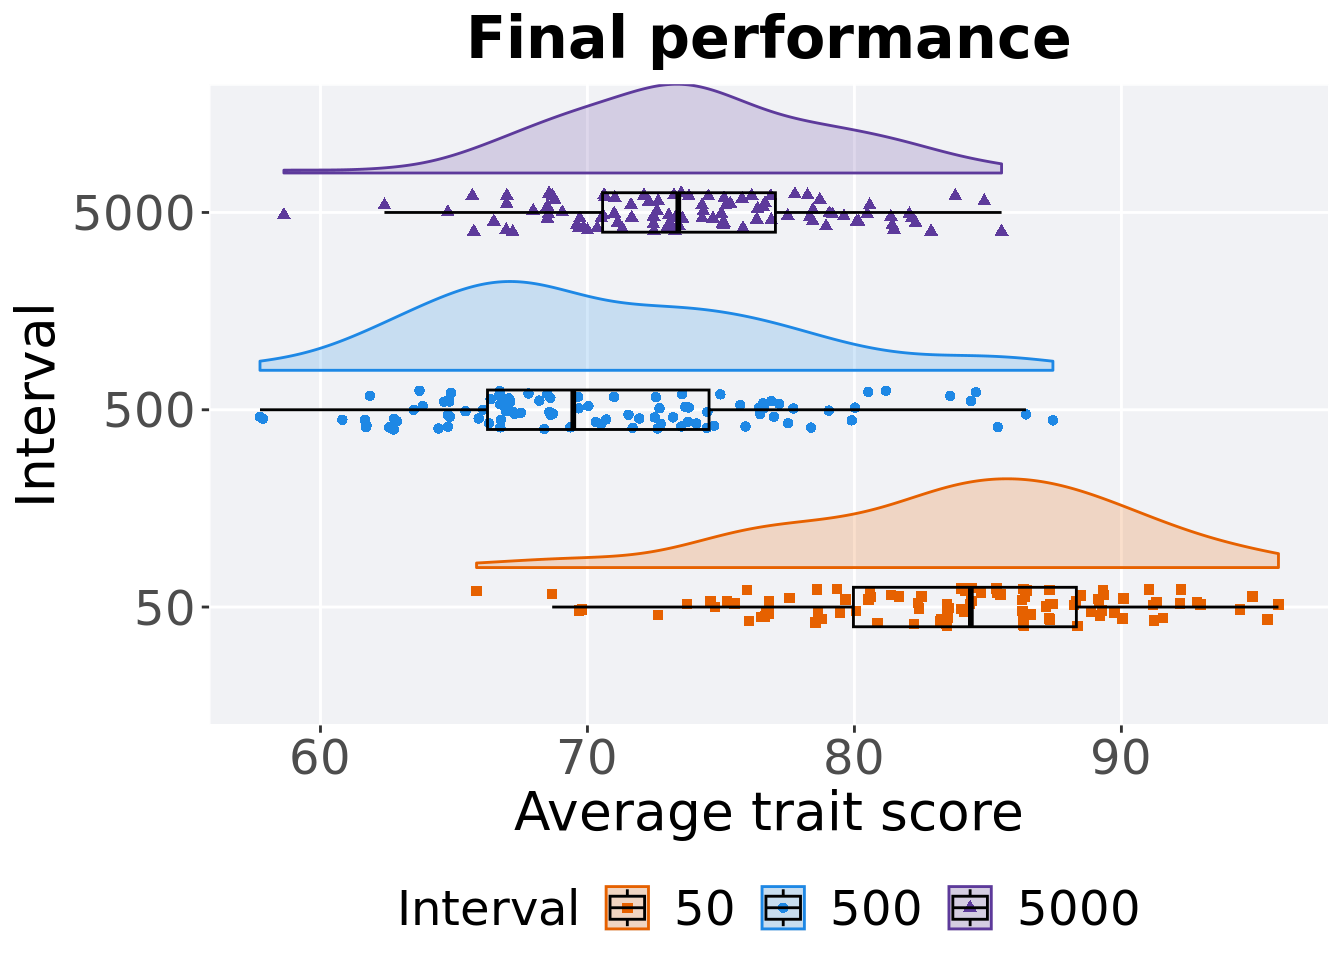
\includegraphics{demo_files/figure-latex/int-lex-mpe-per-end-1.pdf}

\hypertarget{stats-23}{%
\paragraph{Stats}\label{stats-23}}

Summary statistics for the best performance is found throughout in final generation..

\begin{Shaded}
\begin{Highlighting}[]
\NormalTok{performance =}\StringTok{ }\KeywordTok{filter}\NormalTok{(df_ot, Diagnostic }\OperatorTok{==}\StringTok{ 'MULTIPATH_EXPLORATION'} \OperatorTok{&}\StringTok{ `}\DataTypeTok{Selection}\CharTok{\textbackslash{}n}\DataTypeTok{Scheme}\StringTok{`} \OperatorTok{==}\StringTok{ 'LEXICASE'} \OperatorTok{&}\StringTok{ }\NormalTok{Generations }\OperatorTok{==}\StringTok{ }\DecValTok{50000}\NormalTok{)}
\NormalTok{performance}\OperatorTok{$}\NormalTok{Interval =}\StringTok{ }\KeywordTok{factor}\NormalTok{(performance}\OperatorTok{$}\NormalTok{Interval, }\DataTypeTok{levels =} \KeywordTok{c}\NormalTok{(}\StringTok{'50'}\NormalTok{,}\StringTok{'5000'}\NormalTok{,}\StringTok{'500'}\NormalTok{))}
\NormalTok{performance }\OperatorTok
\StringTok{  }\KeywordTok{group_by}\NormalTok{(Interval) }\OperatorTok
\StringTok{  }\NormalTok{dplyr}\OperatorTok{::}\KeywordTok{summarise}\NormalTok{(}
    \DataTypeTok{count =} \KeywordTok{n}\NormalTok{(),}
    \DataTypeTok{na_cnt =} \KeywordTok{sum}\NormalTok{(}\KeywordTok{is.na}\NormalTok{(pop_fit_max)),}
    \DataTypeTok{min =} \KeywordTok{min}\NormalTok{(pop_fit_max }\OperatorTok{/}\StringTok{ }\NormalTok{DIMENSIONALITY, }\DataTypeTok{na.rm =} \OtherTok{TRUE}\NormalTok{),}
    \DataTypeTok{median =} \KeywordTok{median}\NormalTok{(pop_fit_max }\OperatorTok{/}\StringTok{ }\NormalTok{DIMENSIONALITY, }\DataTypeTok{na.rm =} \OtherTok{TRUE}\NormalTok{),}
    \DataTypeTok{mean =} \KeywordTok{mean}\NormalTok{(pop_fit_max }\OperatorTok{/}\StringTok{ }\NormalTok{DIMENSIONALITY, }\DataTypeTok{na.rm =} \OtherTok{TRUE}\NormalTok{),}
    \DataTypeTok{max =} \KeywordTok{max}\NormalTok{(pop_fit_max }\OperatorTok{/}\StringTok{ }\NormalTok{DIMENSIONALITY, }\DataTypeTok{na.rm =} \OtherTok{TRUE}\NormalTok{),}
    \DataTypeTok{IQR =} \KeywordTok{IQR}\NormalTok{(pop_fit_max }\OperatorTok{/}\StringTok{ }\NormalTok{DIMENSIONALITY, }\DataTypeTok{na.rm =} \OtherTok{TRUE}\NormalTok{)}
\NormalTok{  )}
\end{Highlighting}
\end{Shaded}

\begin{verbatim}
## # A tibble: 3 x 8
##   Interval count na_cnt   min median  mean   max   IQR
##   <fct>    <int>  <int> <dbl>  <dbl> <dbl> <dbl> <dbl>
## 1 50         100      0  65.8   84.4  83.9  95.9  8.35
## 2 5000       100      0  58.6   73.4  73.9  85.5  6.47
## 3 500        100      0  57.7   69.5  70.6  87.4  8.30
\end{verbatim}

Kruskal--Wallis test provides evidence of difference among selection schemes.

\begin{Shaded}
\begin{Highlighting}[]
\KeywordTok{kruskal.test}\NormalTok{(pop_fit_max }\OperatorTok{~}\StringTok{ }\NormalTok{Interval, }\DataTypeTok{data =}\NormalTok{ performance)}
\end{Highlighting}
\end{Shaded}

\begin{verbatim}
## 
##  Kruskal-Wallis rank sum test
## 
## data:  pop_fit_max by Interval
## Kruskal-Wallis chi-squared = 140.97, df = 2, p-value < 2.2e-16
\end{verbatim}

Results for post-hoc Wilcoxon rank-sum test with a Bonferroni correction.

\begin{Shaded}
\begin{Highlighting}[]
\KeywordTok{pairwise.wilcox.test}\NormalTok{(}\DataTypeTok{x =}\NormalTok{ performance}\OperatorTok{$}\NormalTok{pop_fit_max, }\DataTypeTok{g =}\NormalTok{ performance}\OperatorTok{$}\NormalTok{Interval, }\DataTypeTok{p.adjust.method =} \StringTok{"bonferroni"}\NormalTok{,}
                     \DataTypeTok{paired =} \OtherTok{FALSE}\NormalTok{, }\DataTypeTok{conf.int =} \OtherTok{FALSE}\NormalTok{, }\DataTypeTok{alternative =} \StringTok{'l'}\NormalTok{)}
\end{Highlighting}
\end{Shaded}

\begin{verbatim}
## 
##  Pairwise comparisons using Wilcoxon rank sum test with continuity correction 
## 
## data:  performance$pop_fit_max and performance$Interval 
## 
##      50      5000   
## 5000 < 2e-16 -      
## 500  < 2e-16 3.8e-05
## 
## P value adjustment method: bonferroni
\end{verbatim}

\hypertarget{activation-gene-coverage-5}{%
\subsection{Activation gene coverage}\label{activation-gene-coverage-5}}

Activation gene coverage analysis.

\hypertarget{coverage-over-time-8}{%
\subsubsection{Coverage over time}\label{coverage-over-time-8}}

Activation gene coverage over time.

\begin{Shaded}
\begin{Highlighting}[]
\CommentTok{# data for lines and shading on plots}
\NormalTok{lines =}\StringTok{ }\KeywordTok{filter}\NormalTok{(df_ot, Diagnostic }\OperatorTok{==}\StringTok{ 'MULTIPATH_EXPLORATION'} \OperatorTok{&}\StringTok{ `}\DataTypeTok{Selection}\CharTok{\textbackslash{}n}\DataTypeTok{Scheme}\StringTok{`} \OperatorTok{==}\StringTok{ 'LEXICASE'}\NormalTok{) }\OperatorTok
\StringTok{  }\KeywordTok{group_by}\NormalTok{(Interval, Generations) }\OperatorTok
\StringTok{  }\NormalTok{dplyr}\OperatorTok{::}\KeywordTok{summarise}\NormalTok{(}
    \DataTypeTok{min =} \KeywordTok{min}\NormalTok{(pop_act_cov),}
    \DataTypeTok{mean =} \KeywordTok{mean}\NormalTok{(pop_act_cov),}
    \DataTypeTok{max =} \KeywordTok{max}\NormalTok{(pop_act_cov)}
\NormalTok{  )}
\end{Highlighting}
\end{Shaded}

\begin{verbatim}
## `summarise()` has grouped output by 'Interval'. You can override using the
## `.groups` argument.
\end{verbatim}

\begin{Shaded}
\begin{Highlighting}[]
\KeywordTok{ggplot}\NormalTok{(lines, }\KeywordTok{aes}\NormalTok{(}\DataTypeTok{x=}\NormalTok{Generations, }\DataTypeTok{y=}\NormalTok{mean, }\DataTypeTok{group =}\NormalTok{ Interval, }\DataTypeTok{fill =}\NormalTok{ Interval, }\DataTypeTok{color =}\NormalTok{ Interval, }\DataTypeTok{shape =}\NormalTok{ Interval)) }\OperatorTok{+}
\StringTok{  }\KeywordTok{geom_ribbon}\NormalTok{(}\KeywordTok{aes}\NormalTok{(}\DataTypeTok{ymin =}\NormalTok{ min, }\DataTypeTok{ymax =}\NormalTok{ max), }\DataTypeTok{alpha =} \FloatTok{0.1}\NormalTok{) }\OperatorTok{+}
\StringTok{  }\KeywordTok{geom_line}\NormalTok{(}\DataTypeTok{size =} \FloatTok{0.5}\NormalTok{) }\OperatorTok{+}
\StringTok{  }\KeywordTok{geom_point}\NormalTok{(}\DataTypeTok{data =} \KeywordTok{filter}\NormalTok{(lines, Generations }\OperatorTok\StringTok{ }\DecValTok{2000} \OperatorTok{==}\StringTok{ }\DecValTok{0}\NormalTok{), }\DataTypeTok{size =} \FloatTok{1.5}\NormalTok{, }\DataTypeTok{stroke =} \FloatTok{2.0}\NormalTok{, }\DataTypeTok{alpha =} \FloatTok{1.0}\NormalTok{) }\OperatorTok{+}
\StringTok{  }\KeywordTok{scale_y_continuous}\NormalTok{(}
    \DataTypeTok{name=}\StringTok{"Coverage"}
\NormalTok{  ) }\OperatorTok{+}
\StringTok{  }\KeywordTok{scale_x_continuous}\NormalTok{(}
    \DataTypeTok{name=}\StringTok{"Generations"}\NormalTok{,}
    \DataTypeTok{limits=}\KeywordTok{c}\NormalTok{(}\DecValTok{0}\NormalTok{, }\DecValTok{50000}\NormalTok{),}
    \DataTypeTok{breaks=}\KeywordTok{c}\NormalTok{(}\DecValTok{0}\NormalTok{, }\DecValTok{10000}\NormalTok{, }\DecValTok{20000}\NormalTok{, }\DecValTok{30000}\NormalTok{, }\DecValTok{40000}\NormalTok{, }\DecValTok{50000}\NormalTok{),}
    \DataTypeTok{labels=}\KeywordTok{c}\NormalTok{(}\StringTok{"0e+4"}\NormalTok{, }\StringTok{"1e+4"}\NormalTok{, }\StringTok{"2e+4"}\NormalTok{, }\StringTok{"3e+4"}\NormalTok{, }\StringTok{"4e+4"}\NormalTok{, }\StringTok{"5e+4"}\NormalTok{)}

\NormalTok{  ) }\OperatorTok{+}
\StringTok{  }\KeywordTok{scale_shape_manual}\NormalTok{(}\DataTypeTok{values=}\NormalTok{SHAPE)}\OperatorTok{+}
\StringTok{  }\KeywordTok{scale_colour_manual}\NormalTok{(}\DataTypeTok{values =}\NormalTok{ cb_palette_mi) }\OperatorTok{+}
\StringTok{  }\KeywordTok{scale_fill_manual}\NormalTok{(}\DataTypeTok{values =}\NormalTok{ cb_palette_mi) }\OperatorTok{+}
\StringTok{  }\KeywordTok{ggtitle}\NormalTok{(}\StringTok{'Activation gene coverage over time'}\NormalTok{)}\OperatorTok{+}
\StringTok{  }\NormalTok{p_theme}
\end{Highlighting}
\end{Shaded}

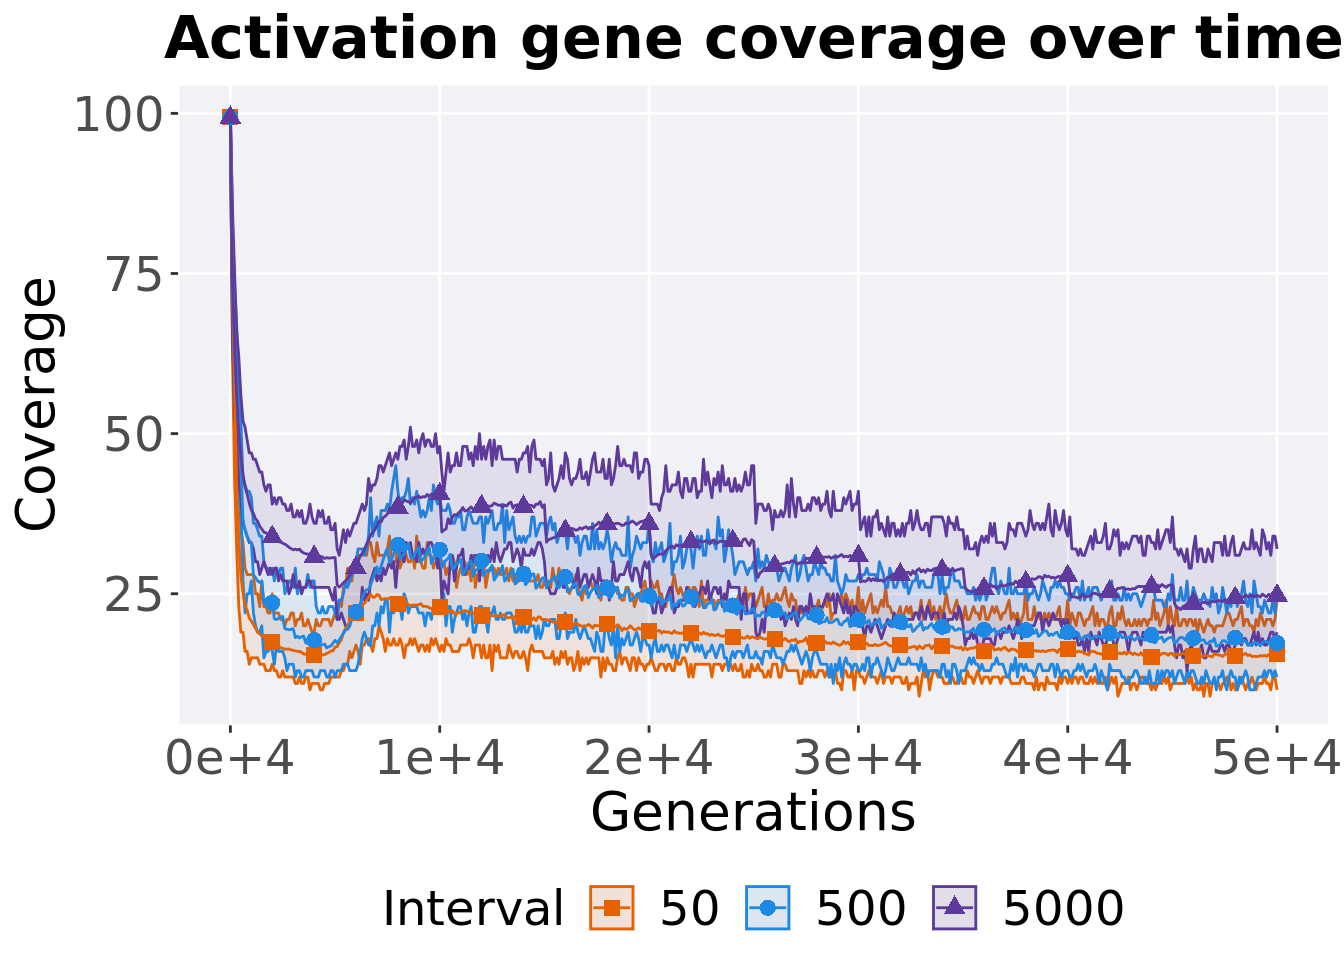
\includegraphics{demo_files/figure-latex/int-mpe-act-lex-ot-1.pdf}

\hypertarget{end-of-50000-generations-8}{%
\subsubsection{End of 50,000 generations}\label{end-of-50000-generations-8}}

Activation gene coverage in the population at the end of 50,000 generations.

\begin{Shaded}
\begin{Highlighting}[]
\CommentTok{### end of run}
\KeywordTok{filter}\NormalTok{(df_ot, Diagnostic }\OperatorTok{==}\StringTok{ 'MULTIPATH_EXPLORATION'} \OperatorTok{&}\StringTok{ `}\DataTypeTok{Selection}\CharTok{\textbackslash{}n}\DataTypeTok{Scheme}\StringTok{`} \OperatorTok{==}\StringTok{ 'LEXICASE'} \OperatorTok{&}\StringTok{ }\NormalTok{Generations }\OperatorTok{==}\StringTok{ }\DecValTok{50000}\NormalTok{) }\OperatorTok
\StringTok{  }\KeywordTok{ggplot}\NormalTok{(., }\KeywordTok{aes}\NormalTok{(}\DataTypeTok{x =}\NormalTok{ Interval, }\DataTypeTok{y =}\NormalTok{ pop_act_cov, }\DataTypeTok{color =}\NormalTok{ Interval, }\DataTypeTok{fill =}\NormalTok{ Interval, }\DataTypeTok{shape =}\NormalTok{ Interval)) }\OperatorTok{+}
\StringTok{  }\KeywordTok{geom_flat_violin}\NormalTok{(}\DataTypeTok{position =} \KeywordTok{position_nudge}\NormalTok{(}\DataTypeTok{x =} \FloatTok{.2}\NormalTok{, }\DataTypeTok{y =} \DecValTok{0}\NormalTok{), }\DataTypeTok{scale =} \StringTok{'width'}\NormalTok{, }\DataTypeTok{alpha =} \FloatTok{0.3}\NormalTok{) }\OperatorTok{+}
\StringTok{  }\KeywordTok{geom_point}\NormalTok{(}\DataTypeTok{position =} \KeywordTok{position_jitter}\NormalTok{(}\DataTypeTok{height =} \FloatTok{.05}\NormalTok{, }\DataTypeTok{width =} \FloatTok{.05}\NormalTok{), }\DataTypeTok{size =} \FloatTok{1.5}\NormalTok{, }\DataTypeTok{alpha =} \FloatTok{0.5}\NormalTok{) }\OperatorTok{+}
\StringTok{  }\KeywordTok{geom_boxplot}\NormalTok{(}\DataTypeTok{color =} \StringTok{'black'}\NormalTok{, }\DataTypeTok{width =} \FloatTok{.2}\NormalTok{, }\DataTypeTok{outlier.shape =} \OtherTok{NA}\NormalTok{, }\DataTypeTok{alpha =} \FloatTok{0.0}\NormalTok{) }\OperatorTok{+}
\StringTok{  }\KeywordTok{scale_shape_manual}\NormalTok{(}\DataTypeTok{values=}\NormalTok{SHAPE)}\OperatorTok{+}
\StringTok{  }\KeywordTok{scale_y_continuous}\NormalTok{(}
    \DataTypeTok{name=}\StringTok{"Coverage"}
\NormalTok{  ) }\OperatorTok{+}
\StringTok{  }\KeywordTok{scale_x_discrete}\NormalTok{(}
    \DataTypeTok{name=}\StringTok{"Interval"}
\NormalTok{  ) }\OperatorTok{+}
\StringTok{  }\KeywordTok{scale_colour_manual}\NormalTok{(}\DataTypeTok{values =}\NormalTok{ cb_palette_mi) }\OperatorTok{+}
\StringTok{  }\KeywordTok{scale_fill_manual}\NormalTok{(}\DataTypeTok{values =}\NormalTok{ cb_palette_mi) }\OperatorTok{+}
\StringTok{  }\KeywordTok{ggtitle}\NormalTok{(}\StringTok{'Final activation gene coverage'}\NormalTok{)}\OperatorTok{+}
\StringTok{  }\NormalTok{p_theme }\OperatorTok{+}\StringTok{ }\KeywordTok{coord_flip}\NormalTok{()}
\end{Highlighting}
\end{Shaded}

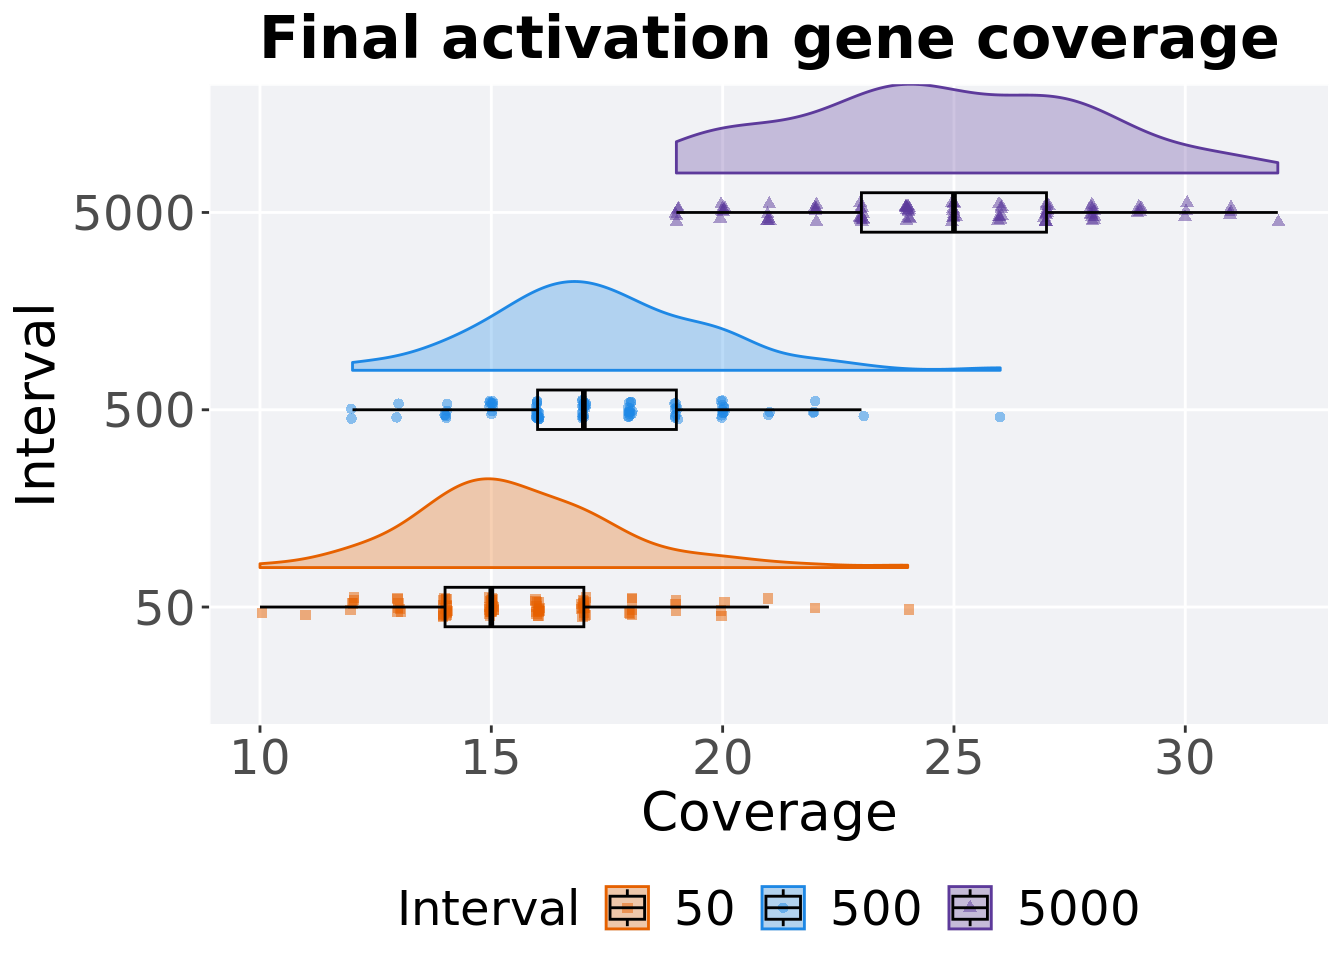
\includegraphics{demo_files/figure-latex/int-mpe-act-lex-end-1.pdf}

\hypertarget{stats-24}{%
\paragraph{Stats}\label{stats-24}}

Summary statistics for activation gene coverage.

\begin{Shaded}
\begin{Highlighting}[]
\NormalTok{coverage =}\StringTok{ }\KeywordTok{filter}\NormalTok{(df_ot, Diagnostic }\OperatorTok{==}\StringTok{ 'MULTIPATH_EXPLORATION'} \OperatorTok{&}\StringTok{ `}\DataTypeTok{Selection}\CharTok{\textbackslash{}n}\DataTypeTok{Scheme}\StringTok{`} \OperatorTok{==}\StringTok{ 'LEXICASE'} \OperatorTok{&}\StringTok{ }\NormalTok{Generations }\OperatorTok{==}\StringTok{ }\DecValTok{50000}\NormalTok{)}
\NormalTok{coverage}\OperatorTok{$}\NormalTok{Interval =}\StringTok{ }\KeywordTok{factor}\NormalTok{(coverage}\OperatorTok{$}\NormalTok{Interval, }\DataTypeTok{levels =} \KeywordTok{c}\NormalTok{(}\StringTok{'50'}\NormalTok{,}\StringTok{'500'}\NormalTok{,}\StringTok{'5000'}\NormalTok{))}
\NormalTok{coverage }\OperatorTok
\StringTok{  }\KeywordTok{group_by}\NormalTok{(Interval) }\OperatorTok
\StringTok{  }\NormalTok{dplyr}\OperatorTok{::}\KeywordTok{summarise}\NormalTok{(}
    \DataTypeTok{count =} \KeywordTok{n}\NormalTok{(),}
    \DataTypeTok{na_cnt =} \KeywordTok{sum}\NormalTok{(}\KeywordTok{is.na}\NormalTok{(pop_act_cov)),}
    \DataTypeTok{min =} \KeywordTok{min}\NormalTok{(pop_act_cov, }\DataTypeTok{na.rm =} \OtherTok{TRUE}\NormalTok{),}
    \DataTypeTok{median =} \KeywordTok{median}\NormalTok{(pop_act_cov, }\DataTypeTok{na.rm =} \OtherTok{TRUE}\NormalTok{),}
    \DataTypeTok{mean =} \KeywordTok{mean}\NormalTok{(pop_act_cov, }\DataTypeTok{na.rm =} \OtherTok{TRUE}\NormalTok{),}
    \DataTypeTok{max =} \KeywordTok{max}\NormalTok{(pop_act_cov, }\DataTypeTok{na.rm =} \OtherTok{TRUE}\NormalTok{),}
    \DataTypeTok{IQR =} \KeywordTok{IQR}\NormalTok{(pop_act_cov, }\DataTypeTok{na.rm =} \OtherTok{TRUE}\NormalTok{)}
\NormalTok{  )}
\end{Highlighting}
\end{Shaded}

\begin{verbatim}
## # A tibble: 3 x 8
##   Interval count na_cnt   min median  mean   max   IQR
##   <fct>    <int>  <int> <int>  <dbl> <dbl> <int> <dbl>
## 1 50         100      0    10     15  15.6    24     3
## 2 500        100      0    12     17  17.3    26     3
## 3 5000       100      0    19     25  24.8    32     4
\end{verbatim}

Kruskal--Wallis test provides evidence of difference among activation gene coverage.

\begin{Shaded}
\begin{Highlighting}[]
\KeywordTok{kruskal.test}\NormalTok{(pop_act_cov }\OperatorTok{~}\StringTok{ }\NormalTok{Interval, }\DataTypeTok{data =}\NormalTok{ coverage)}
\end{Highlighting}
\end{Shaded}

\begin{verbatim}
## 
##  Kruskal-Wallis rank sum test
## 
## data:  pop_act_cov by Interval
## Kruskal-Wallis chi-squared = 198.08, df = 2, p-value < 2.2e-16
\end{verbatim}

Results for post-hoc Wilcoxon rank-sum test with a Bonferroni correction on activation gene coverage.

\begin{Shaded}
\begin{Highlighting}[]
\KeywordTok{pairwise.wilcox.test}\NormalTok{(}\DataTypeTok{x =}\NormalTok{ coverage}\OperatorTok{$}\NormalTok{pop_act_cov, }\DataTypeTok{g =}\NormalTok{ coverage}\OperatorTok{$}\NormalTok{Interval, }\DataTypeTok{p.adjust.method =} \StringTok{"bonferroni"}\NormalTok{,}
                     \DataTypeTok{paired =} \OtherTok{FALSE}\NormalTok{, }\DataTypeTok{conf.int =} \OtherTok{FALSE}\NormalTok{, }\DataTypeTok{alternative =} \StringTok{'g'}\NormalTok{)}
\end{Highlighting}
\end{Shaded}

\begin{verbatim}
## 
##  Pairwise comparisons using Wilcoxon rank sum test with continuity correction 
## 
## data:  coverage$pop_act_cov and coverage$Interval 
## 
##      50      500    
## 500  1.3e-07 -      
## 5000 < 2e-16 < 2e-16
## 
## P value adjustment method: bonferroni
\end{verbatim}

\hypertarget{mi500-exploitation-rate-results}{%
\chapter{MI500: Exploitation rate results}\label{mi500-exploitation-rate-results}}

Here we present the results for \textbf{best performances} found by each selection scheme replicate on the exploitation rate diagnostic with our base configurations.
For our base configuration, we assume that there are migrations every 500 generations, 4 islands, and a ring topology.
When migrations occur, we swap two individuals (same position on each island) and guarantee that no solution can return to the same island.
Best performance found refers to the largest average trait score found in a given population.
Note that performance values fall between 0.0 and 100.0.

\hypertarget{analysis-dependencies-4}{%
\section{Analysis dependencies}\label{analysis-dependencies-4}}

\begin{Shaded}
\begin{Highlighting}[]
\KeywordTok{library}\NormalTok{(ggplot2)}
\KeywordTok{library}\NormalTok{(cowplot)}
\KeywordTok{library}\NormalTok{(dplyr)}
\KeywordTok{library}\NormalTok{(PupillometryR)}
\end{Highlighting}
\end{Shaded}

\hypertarget{truncation-selection-4}{%
\section{Truncation selection}\label{truncation-selection-4}}

Here we analyze how the different population structures affect truncation selection (size 8) on the exploitation rate diagnostic.

\hypertarget{performance-over-time-9}{%
\subsection{Performance over time}\label{performance-over-time-9}}

\begin{Shaded}
\begin{Highlighting}[]
\NormalTok{lines =}\StringTok{ }\KeywordTok{filter}\NormalTok{(base_over_time, Diagnostic }\OperatorTok{==}\StringTok{ 'EXPLOITATION_RATE'} \OperatorTok{&}\StringTok{ `}\DataTypeTok{Selection}\CharTok{\textbackslash{}n}\DataTypeTok{Scheme}\StringTok{`} \OperatorTok{==}\StringTok{ 'TRUNCATION'}\NormalTok{) }\OperatorTok
\StringTok{  }\KeywordTok{group_by}\NormalTok{(Structure, Generations) }\OperatorTok
\StringTok{  }\NormalTok{dplyr}\OperatorTok{::}\KeywordTok{summarise}\NormalTok{(}
    \DataTypeTok{min =} \KeywordTok{min}\NormalTok{(pop_fit_max) }\OperatorTok{/}\StringTok{ }\NormalTok{DIMENSIONALITY,}
    \DataTypeTok{mean =} \KeywordTok{mean}\NormalTok{(pop_fit_max) }\OperatorTok{/}\StringTok{ }\NormalTok{DIMENSIONALITY,}
    \DataTypeTok{max =} \KeywordTok{max}\NormalTok{(pop_fit_max) }\OperatorTok{/}\StringTok{ }\NormalTok{DIMENSIONALITY}
\NormalTok{  )}
\KeywordTok{ggplot}\NormalTok{(lines, }\KeywordTok{aes}\NormalTok{(}\DataTypeTok{x=}\NormalTok{Generations, }\DataTypeTok{y=}\NormalTok{mean, }\DataTypeTok{group =}\NormalTok{ Structure, }\DataTypeTok{fill =}\NormalTok{ Structure, }\DataTypeTok{color =}\NormalTok{ Structure, }\DataTypeTok{shape =}\NormalTok{ Structure)) }\OperatorTok{+}
\StringTok{  }\KeywordTok{geom_ribbon}\NormalTok{(}\KeywordTok{aes}\NormalTok{(}\DataTypeTok{ymin =}\NormalTok{ min, }\DataTypeTok{ymax =}\NormalTok{ max), }\DataTypeTok{alpha =} \FloatTok{0.1}\NormalTok{) }\OperatorTok{+}
\StringTok{  }\KeywordTok{geom_line}\NormalTok{(}\DataTypeTok{size =} \FloatTok{0.5}\NormalTok{) }\OperatorTok{+}
\StringTok{  }\KeywordTok{geom_point}\NormalTok{(}\DataTypeTok{data =} \KeywordTok{filter}\NormalTok{(lines, Generations }\OperatorTok\StringTok{ }\DecValTok{2000} \OperatorTok{==}\StringTok{ }\DecValTok{0}\NormalTok{), }\DataTypeTok{size =} \FloatTok{2.5}\NormalTok{, }\DataTypeTok{stroke =} \FloatTok{2.0}\NormalTok{, }\DataTypeTok{alpha =} \FloatTok{1.0}\NormalTok{) }\OperatorTok{+}
\StringTok{  }\KeywordTok{scale_y_continuous}\NormalTok{(}
    \DataTypeTok{name=}\StringTok{"Average trait score"}\NormalTok{,}
    \DataTypeTok{limits=}\KeywordTok{c}\NormalTok{(}\OperatorTok{-}\DecValTok{1}\NormalTok{, }\DecValTok{101}\NormalTok{),}
    \DataTypeTok{breaks=}\KeywordTok{seq}\NormalTok{(}\DecValTok{0}\NormalTok{,}\DecValTok{100}\NormalTok{, }\DecValTok{20}\NormalTok{),}
    \DataTypeTok{labels=}\KeywordTok{c}\NormalTok{(}\StringTok{"0"}\NormalTok{, }\StringTok{"20"}\NormalTok{, }\StringTok{"40"}\NormalTok{, }\StringTok{"60"}\NormalTok{, }\StringTok{"80"}\NormalTok{, }\StringTok{"100"}\NormalTok{)}
\NormalTok{  ) }\OperatorTok{+}
\StringTok{  }\KeywordTok{scale_x_continuous}\NormalTok{(}
    \DataTypeTok{name=}\StringTok{"Generations"}\NormalTok{,}
    \DataTypeTok{limits=}\KeywordTok{c}\NormalTok{(}\DecValTok{0}\NormalTok{, }\DecValTok{50000}\NormalTok{),}
    \DataTypeTok{breaks=}\KeywordTok{c}\NormalTok{(}\DecValTok{0}\NormalTok{, }\DecValTok{10000}\NormalTok{, }\DecValTok{20000}\NormalTok{, }\DecValTok{30000}\NormalTok{, }\DecValTok{40000}\NormalTok{, }\DecValTok{50000}\NormalTok{),}
    \DataTypeTok{labels=}\KeywordTok{c}\NormalTok{(}\StringTok{"0e+4"}\NormalTok{, }\StringTok{"1e+4"}\NormalTok{, }\StringTok{"2e+4"}\NormalTok{, }\StringTok{"3e+4"}\NormalTok{, }\StringTok{"4e+4"}\NormalTok{, }\StringTok{"5e+4"}\NormalTok{)}

\NormalTok{  ) }\OperatorTok{+}
\StringTok{  }\KeywordTok{scale_shape_manual}\NormalTok{(}\DataTypeTok{values=}\NormalTok{SHAPE)}\OperatorTok{+}
\StringTok{  }\KeywordTok{scale_colour_manual}\NormalTok{(}\DataTypeTok{values =}\NormalTok{ cb_palette) }\OperatorTok{+}
\StringTok{  }\KeywordTok{scale_fill_manual}\NormalTok{(}\DataTypeTok{values =}\NormalTok{ cb_palette) }\OperatorTok{+}
\StringTok{  }\KeywordTok{ggtitle}\NormalTok{(}\StringTok{"Best performance over time"}\NormalTok{) }\OperatorTok{+}
\StringTok{  }\NormalTok{p_theme}
\end{Highlighting}
\end{Shaded}

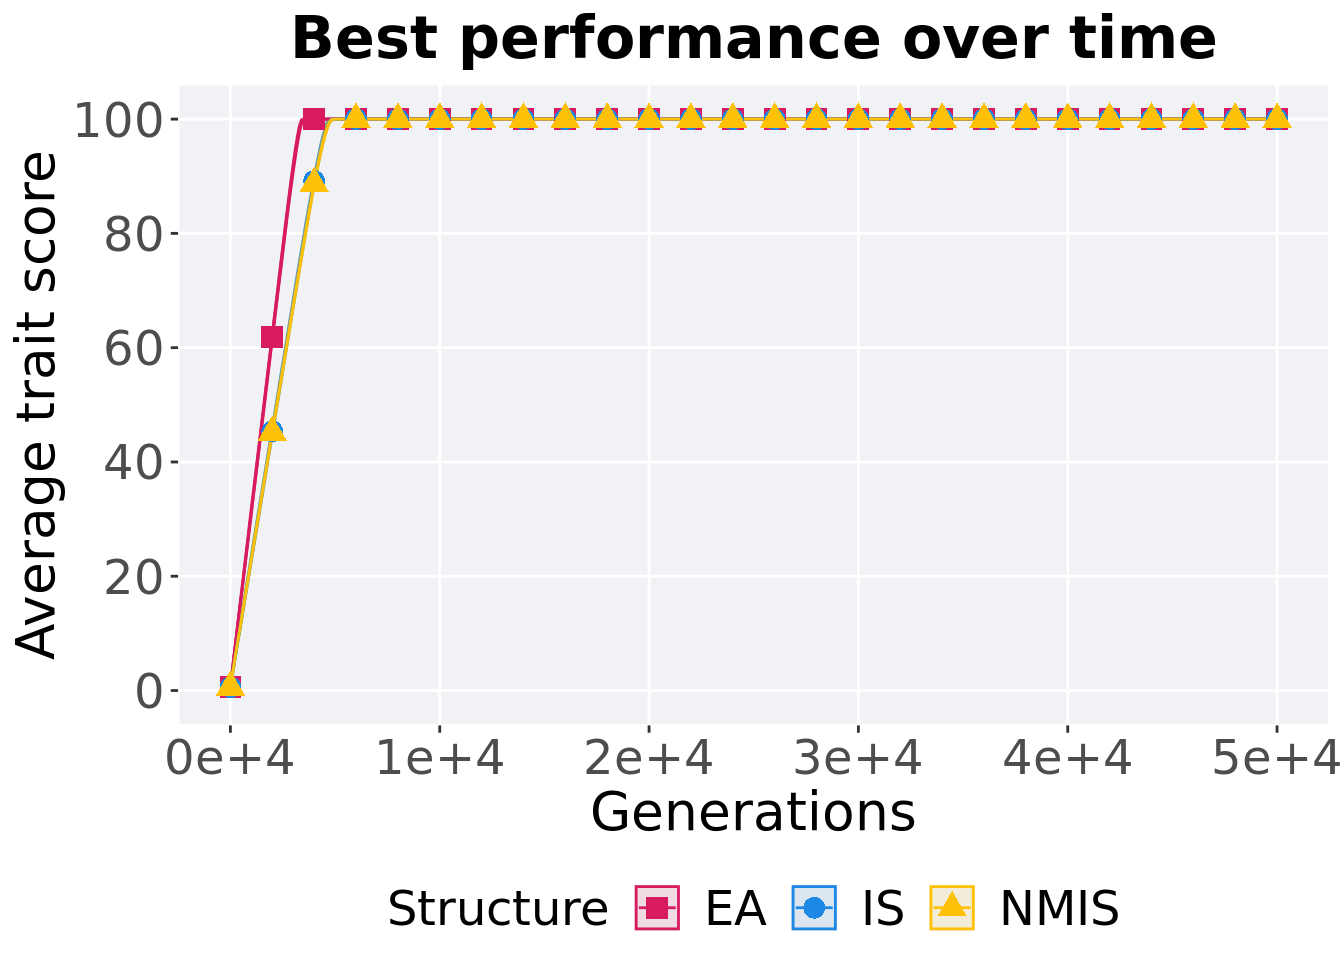
\includegraphics{demo_files/figure-latex/base-tru-exp-perf-1.pdf}

\hypertarget{generation-satisfactory-solution-found-6}{%
\subsection{Generation satisfactory solution found}\label{generation-satisfactory-solution-found-6}}

First generation a satisfactory solution is found throughout the 50,000 generations.

\begin{Shaded}
\begin{Highlighting}[]
\KeywordTok{filter}\NormalTok{(base_ssf, Diagnostic }\OperatorTok{==}\StringTok{ 'EXPLOITATION_RATE'} \OperatorTok{&}\StringTok{ `}\DataTypeTok{Selection}\CharTok{\textbackslash{}n}\DataTypeTok{Scheme}\StringTok{`} \OperatorTok{==}\StringTok{ 'TRUNCATION'}\NormalTok{) }\OperatorTok
\StringTok{  }\KeywordTok{ggplot}\NormalTok{(., }\KeywordTok{aes}\NormalTok{(}\DataTypeTok{x =}\NormalTok{ Structure, }\DataTypeTok{y =}\NormalTok{ Generations , }\DataTypeTok{color =}\NormalTok{ Structure, }\DataTypeTok{fill =}\NormalTok{ Structure, }\DataTypeTok{shape =}\NormalTok{ Structure)) }\OperatorTok{+}
\StringTok{  }\KeywordTok{geom_flat_violin}\NormalTok{(}\DataTypeTok{position =} \KeywordTok{position_nudge}\NormalTok{(}\DataTypeTok{x =} \FloatTok{.2}\NormalTok{, }\DataTypeTok{y =} \DecValTok{0}\NormalTok{), }\DataTypeTok{scale =} \StringTok{'width'}\NormalTok{, }\DataTypeTok{alpha =} \FloatTok{0.2}\NormalTok{) }\OperatorTok{+}
\StringTok{  }\KeywordTok{geom_point}\NormalTok{(}\DataTypeTok{position =} \KeywordTok{position_jitter}\NormalTok{(}\DataTypeTok{width =} \FloatTok{.1}\NormalTok{), }\DataTypeTok{size =} \FloatTok{1.5}\NormalTok{, }\DataTypeTok{alpha =} \FloatTok{1.0}\NormalTok{) }\OperatorTok{+}
\StringTok{  }\KeywordTok{geom_boxplot}\NormalTok{(}\DataTypeTok{color =} \StringTok{'black'}\NormalTok{, }\DataTypeTok{width =} \FloatTok{.2}\NormalTok{, }\DataTypeTok{outlier.shape =} \OtherTok{NA}\NormalTok{, }\DataTypeTok{alpha =} \FloatTok{0.0}\NormalTok{) }\OperatorTok{+}
\StringTok{  }\KeywordTok{scale_y_continuous}\NormalTok{(}
    \DataTypeTok{name=}\StringTok{"Generation"}
\NormalTok{  ) }\OperatorTok{+}
\StringTok{  }\KeywordTok{scale_x_discrete}\NormalTok{(}
    \DataTypeTok{name=}\StringTok{"Structure"}
\NormalTok{  )}\OperatorTok{+}
\StringTok{  }\KeywordTok{scale_shape_manual}\NormalTok{(}\DataTypeTok{values=}\NormalTok{SHAPE)}\OperatorTok{+}
\StringTok{  }\KeywordTok{scale_colour_manual}\NormalTok{(}\DataTypeTok{values =}\NormalTok{ cb_palette, ) }\OperatorTok{+}
\StringTok{  }\KeywordTok{scale_fill_manual}\NormalTok{(}\DataTypeTok{values =}\NormalTok{ cb_palette) }\OperatorTok{+}
\StringTok{  }\KeywordTok{ggtitle}\NormalTok{(}\StringTok{'Generation satisfactory solution found'}\NormalTok{)}\OperatorTok{+}
\StringTok{  }\NormalTok{p_theme }\OperatorTok{+}\StringTok{ }\KeywordTok{coord_flip}\NormalTok{()}
\end{Highlighting}
\end{Shaded}

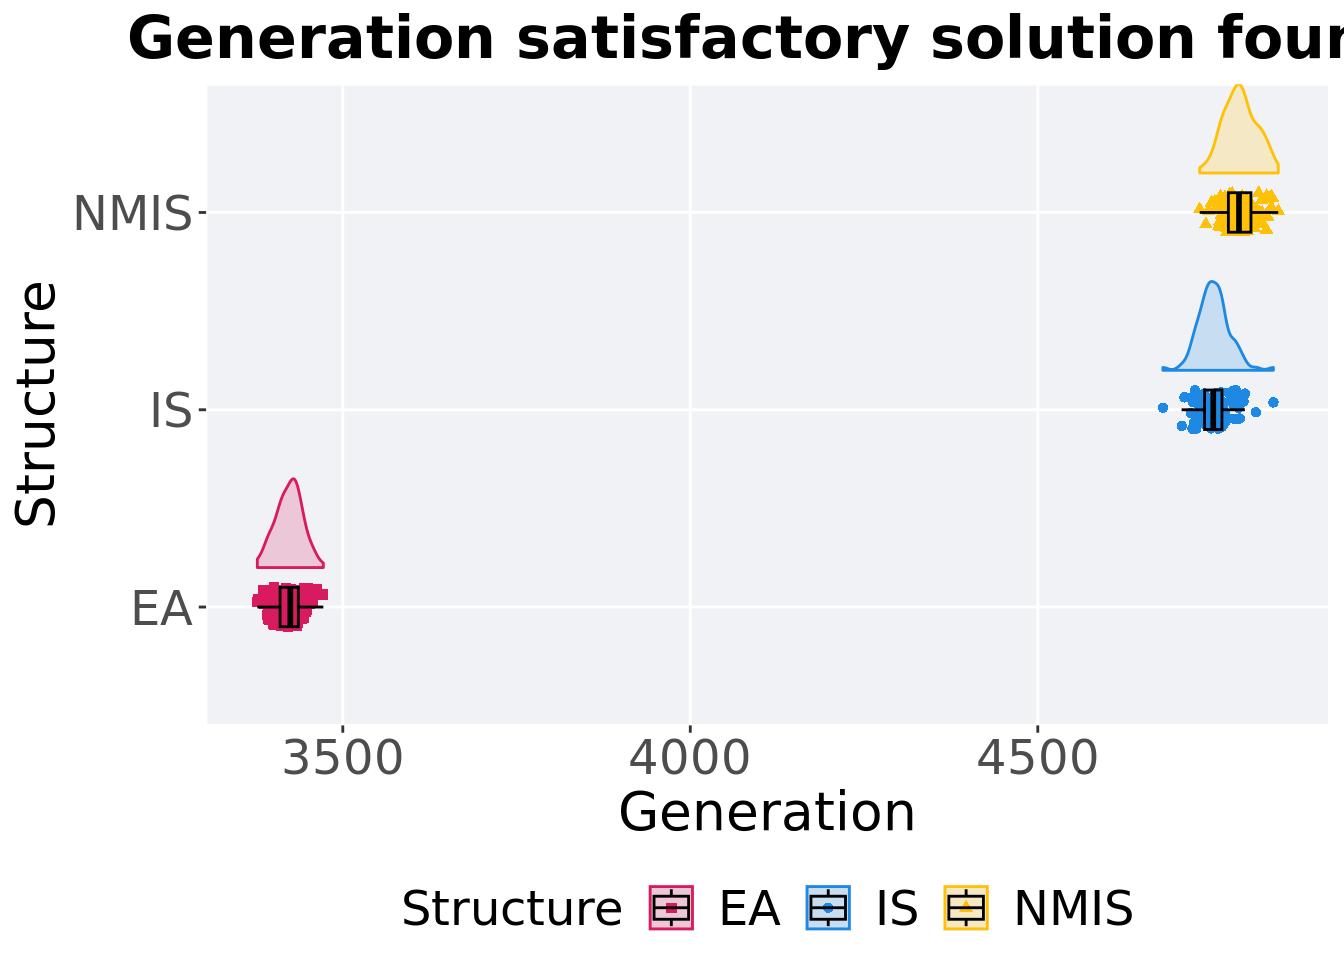
\includegraphics{demo_files/figure-latex/base-tru-exp-ssf-1.pdf}

\hypertarget{stats-25}{%
\subsection{Stats}\label{stats-25}}

Summary statistics for the first generation a satisfactory solution is found.

\begin{Shaded}
\begin{Highlighting}[]
\NormalTok{ssf =}\StringTok{ }\KeywordTok{filter}\NormalTok{(base_ssf, Diagnostic }\OperatorTok{==}\StringTok{ 'EXPLOITATION_RATE'} \OperatorTok{&}\StringTok{ `}\DataTypeTok{Selection}\CharTok{\textbackslash{}n}\DataTypeTok{Scheme}\StringTok{`} \OperatorTok{==}\StringTok{ 'TRUNCATION'} \OperatorTok{&}\StringTok{ }\NormalTok{Generations }\OperatorTok{<}\StringTok{ }\DecValTok{60000}\NormalTok{)}
\NormalTok{ssf }\OperatorTok
\StringTok{  }\KeywordTok{group_by}\NormalTok{(Structure) }\OperatorTok
\StringTok{  }\NormalTok{dplyr}\OperatorTok{::}\KeywordTok{summarise}\NormalTok{(}
    \DataTypeTok{count =} \KeywordTok{n}\NormalTok{(),}
    \DataTypeTok{na_cnt =} \KeywordTok{sum}\NormalTok{(}\KeywordTok{is.na}\NormalTok{(Generations)),}
    \DataTypeTok{min =} \KeywordTok{min}\NormalTok{(Generations, }\DataTypeTok{na.rm =} \OtherTok{TRUE}\NormalTok{),}
    \DataTypeTok{median =} \KeywordTok{median}\NormalTok{(Generations, }\DataTypeTok{na.rm =} \OtherTok{TRUE}\NormalTok{),}
    \DataTypeTok{mean =} \KeywordTok{mean}\NormalTok{(Generations, }\DataTypeTok{na.rm =} \OtherTok{TRUE}\NormalTok{),}
    \DataTypeTok{max =} \KeywordTok{max}\NormalTok{(Generations, }\DataTypeTok{na.rm =} \OtherTok{TRUE}\NormalTok{),}
    \DataTypeTok{IQR =} \KeywordTok{IQR}\NormalTok{(Generations, }\DataTypeTok{na.rm =} \OtherTok{TRUE}\NormalTok{)}
\NormalTok{  )}
\end{Highlighting}
\end{Shaded}

\begin{verbatim}
## # A tibble: 3 x 8
##   Structure count na_cnt   min median  mean   max   IQR
##   <fct>     <int>  <int> <int>  <dbl> <dbl> <int> <dbl>
## 1 EA          100      0  3377  3424. 3423.  3472  26.2
## 2 IS          100      0  4680  4752. 4754.  4839  25  
## 3 NMIS        100      0  4733  4790. 4791.  4846  32.5
\end{verbatim}

Kruskal--Wallis test provides evidence of difference among selection schemes.

\begin{Shaded}
\begin{Highlighting}[]
\KeywordTok{kruskal.test}\NormalTok{(Generations }\OperatorTok{~}\StringTok{ }\NormalTok{Structure, }\DataTypeTok{data =}\NormalTok{ ssf)}
\end{Highlighting}
\end{Shaded}

\begin{verbatim}
## 
##  Kruskal-Wallis rank sum test
## 
## data:  Generations by Structure
## Kruskal-Wallis chi-squared = 237.99, df = 2, p-value < 2.2e-16
\end{verbatim}

Results for post-hoc Wilcoxon rank-sum test with a Bonferroni correction.

\begin{Shaded}
\begin{Highlighting}[]
\KeywordTok{pairwise.wilcox.test}\NormalTok{(}\DataTypeTok{x =}\NormalTok{ ssf}\OperatorTok{$}\NormalTok{Generations, }\DataTypeTok{g =}\NormalTok{ ssf}\OperatorTok{$}\NormalTok{Structure, }\DataTypeTok{p.adjust.method =} \StringTok{"bonferroni"}\NormalTok{,}
                     \DataTypeTok{paired =} \OtherTok{FALSE}\NormalTok{, }\DataTypeTok{conf.int =} \OtherTok{FALSE}\NormalTok{, }\DataTypeTok{alternative =} \StringTok{'g'}\NormalTok{)}
\end{Highlighting}
\end{Shaded}

\begin{verbatim}
## 
##  Pairwise comparisons using Wilcoxon rank sum test with continuity correction 
## 
## data:  ssf$Generations and ssf$Structure 
## 
##      EA     IS    
## IS   <2e-16 -     
## NMIS <2e-16 <2e-16
## 
## P value adjustment method: bonferroni
\end{verbatim}

\hypertarget{tournament-selection-4}{%
\section{Tournament selection}\label{tournament-selection-4}}

Here we analyze how the different population structures affect tournament selection (size 8) on the exploitation rate diagnostic.

\hypertarget{performance-over-time-10}{%
\subsection{Performance over time}\label{performance-over-time-10}}

\begin{Shaded}
\begin{Highlighting}[]
\NormalTok{lines =}\StringTok{ }\KeywordTok{filter}\NormalTok{(base_over_time, Diagnostic }\OperatorTok{==}\StringTok{ 'EXPLOITATION_RATE'} \OperatorTok{&}\StringTok{ `}\DataTypeTok{Selection}\CharTok{\textbackslash{}n}\DataTypeTok{Scheme}\StringTok{`} \OperatorTok{==}\StringTok{ 'TOURNAMENT'}\NormalTok{) }\OperatorTok
\StringTok{  }\KeywordTok{group_by}\NormalTok{(Structure, Generations) }\OperatorTok
\StringTok{  }\NormalTok{dplyr}\OperatorTok{::}\KeywordTok{summarise}\NormalTok{(}
    \DataTypeTok{min =} \KeywordTok{min}\NormalTok{(pop_fit_max) }\OperatorTok{/}\StringTok{ }\NormalTok{DIMENSIONALITY,}
    \DataTypeTok{mean =} \KeywordTok{mean}\NormalTok{(pop_fit_max) }\OperatorTok{/}\StringTok{ }\NormalTok{DIMENSIONALITY,}
    \DataTypeTok{max =} \KeywordTok{max}\NormalTok{(pop_fit_max) }\OperatorTok{/}\StringTok{ }\NormalTok{DIMENSIONALITY}
\NormalTok{  )}
\KeywordTok{ggplot}\NormalTok{(lines, }\KeywordTok{aes}\NormalTok{(}\DataTypeTok{x=}\NormalTok{Generations, }\DataTypeTok{y=}\NormalTok{mean, }\DataTypeTok{group =}\NormalTok{ Structure, }\DataTypeTok{fill =}\NormalTok{ Structure, }\DataTypeTok{color =}\NormalTok{ Structure, }\DataTypeTok{shape =}\NormalTok{ Structure)) }\OperatorTok{+}
\StringTok{  }\KeywordTok{geom_ribbon}\NormalTok{(}\KeywordTok{aes}\NormalTok{(}\DataTypeTok{ymin =}\NormalTok{ min, }\DataTypeTok{ymax =}\NormalTok{ max), }\DataTypeTok{alpha =} \FloatTok{0.1}\NormalTok{) }\OperatorTok{+}
\StringTok{  }\KeywordTok{geom_line}\NormalTok{(}\DataTypeTok{size =} \FloatTok{0.5}\NormalTok{) }\OperatorTok{+}
\StringTok{  }\KeywordTok{geom_point}\NormalTok{(}\DataTypeTok{data =} \KeywordTok{filter}\NormalTok{(lines, Generations }\OperatorTok\StringTok{ }\DecValTok{2000} \OperatorTok{==}\StringTok{ }\DecValTok{0}\NormalTok{), }\DataTypeTok{size =} \FloatTok{2.5}\NormalTok{, }\DataTypeTok{stroke =} \FloatTok{2.0}\NormalTok{, }\DataTypeTok{alpha =} \FloatTok{1.0}\NormalTok{) }\OperatorTok{+}
\StringTok{  }\KeywordTok{scale_y_continuous}\NormalTok{(}
    \DataTypeTok{name=}\StringTok{"Average trait score"}\NormalTok{,}
    \DataTypeTok{limits=}\KeywordTok{c}\NormalTok{(}\OperatorTok{-}\DecValTok{1}\NormalTok{, }\DecValTok{101}\NormalTok{),}
    \DataTypeTok{breaks=}\KeywordTok{seq}\NormalTok{(}\DecValTok{0}\NormalTok{,}\DecValTok{100}\NormalTok{, }\DecValTok{20}\NormalTok{),}
    \DataTypeTok{labels=}\KeywordTok{c}\NormalTok{(}\StringTok{"0"}\NormalTok{, }\StringTok{"20"}\NormalTok{, }\StringTok{"40"}\NormalTok{, }\StringTok{"60"}\NormalTok{, }\StringTok{"80"}\NormalTok{, }\StringTok{"100"}\NormalTok{)}
\NormalTok{  ) }\OperatorTok{+}
\StringTok{  }\KeywordTok{scale_x_continuous}\NormalTok{(}
    \DataTypeTok{name=}\StringTok{"Generations"}\NormalTok{,}
    \DataTypeTok{limits=}\KeywordTok{c}\NormalTok{(}\DecValTok{0}\NormalTok{, }\DecValTok{50000}\NormalTok{),}
    \DataTypeTok{breaks=}\KeywordTok{c}\NormalTok{(}\DecValTok{0}\NormalTok{, }\DecValTok{10000}\NormalTok{, }\DecValTok{20000}\NormalTok{, }\DecValTok{30000}\NormalTok{, }\DecValTok{40000}\NormalTok{, }\DecValTok{50000}\NormalTok{),}
    \DataTypeTok{labels=}\KeywordTok{c}\NormalTok{(}\StringTok{"0e+4"}\NormalTok{, }\StringTok{"1e+4"}\NormalTok{, }\StringTok{"2e+4"}\NormalTok{, }\StringTok{"3e+4"}\NormalTok{, }\StringTok{"4e+4"}\NormalTok{, }\StringTok{"5e+4"}\NormalTok{)}

\NormalTok{  ) }\OperatorTok{+}
\StringTok{  }\KeywordTok{scale_shape_manual}\NormalTok{(}\DataTypeTok{values=}\NormalTok{SHAPE)}\OperatorTok{+}
\StringTok{  }\KeywordTok{scale_colour_manual}\NormalTok{(}\DataTypeTok{values =}\NormalTok{ cb_palette) }\OperatorTok{+}
\StringTok{  }\KeywordTok{scale_fill_manual}\NormalTok{(}\DataTypeTok{values =}\NormalTok{ cb_palette) }\OperatorTok{+}
\StringTok{  }\KeywordTok{ggtitle}\NormalTok{(}\StringTok{"Best performance over time"}\NormalTok{) }\OperatorTok{+}
\StringTok{  }\NormalTok{p_theme}
\end{Highlighting}
\end{Shaded}

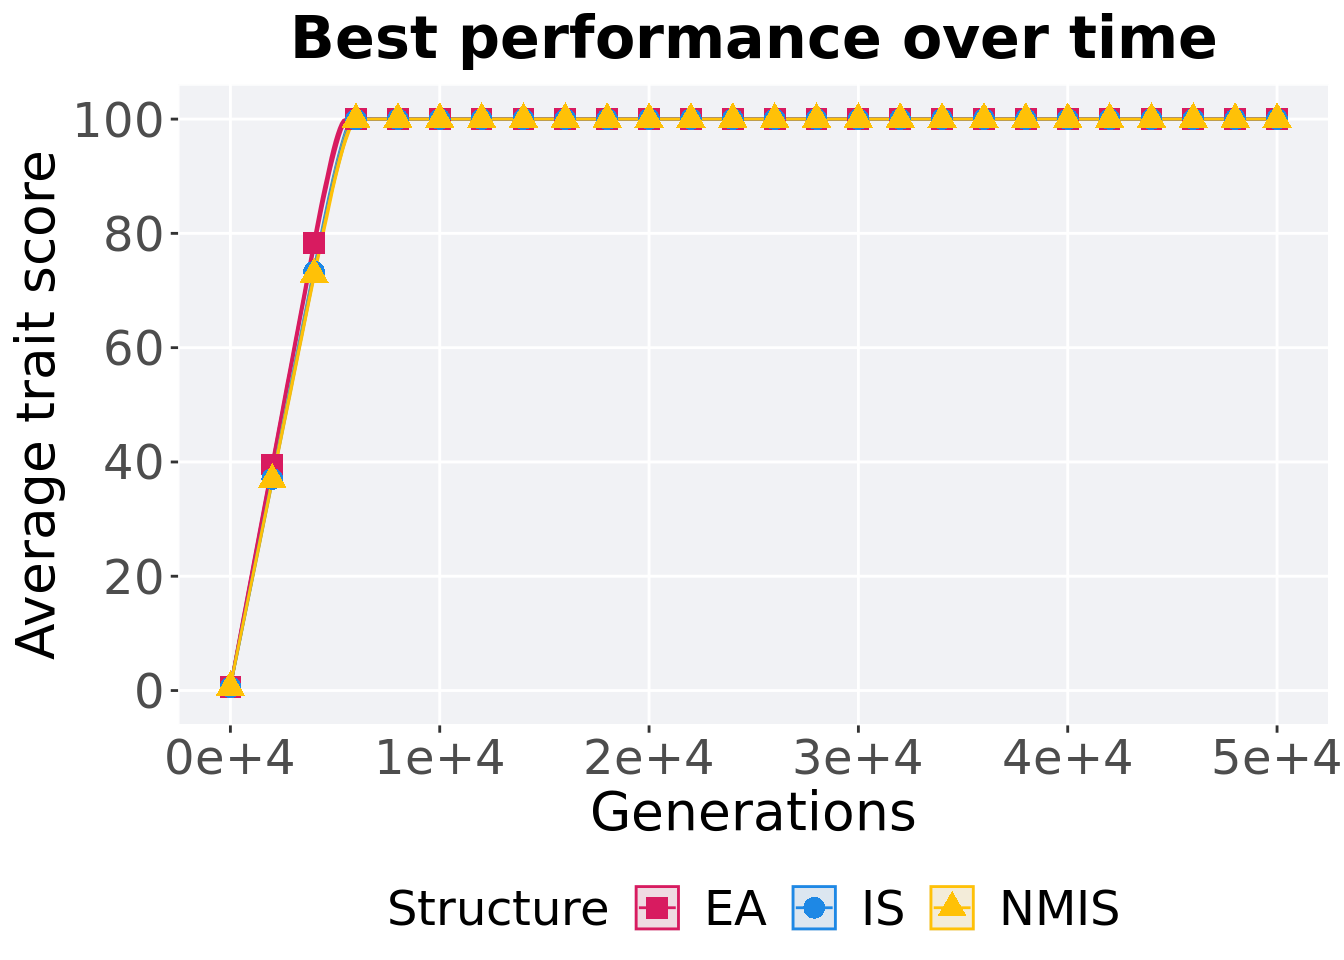
\includegraphics{demo_files/figure-latex/base-tor-exp-perf-1.pdf}

\hypertarget{generation-satisfactory-solution-found-7}{%
\subsection{Generation satisfactory solution found}\label{generation-satisfactory-solution-found-7}}

First generation a satisfactory solution is found throughout the 50,000 generations.

\begin{Shaded}
\begin{Highlighting}[]
\KeywordTok{filter}\NormalTok{(base_ssf, Diagnostic }\OperatorTok{==}\StringTok{ 'EXPLOITATION_RATE'} \OperatorTok{&}\StringTok{ `}\DataTypeTok{Selection}\CharTok{\textbackslash{}n}\DataTypeTok{Scheme}\StringTok{`} \OperatorTok{==}\StringTok{ 'TOURNAMENT'}\NormalTok{) }\OperatorTok
\StringTok{  }\KeywordTok{ggplot}\NormalTok{(., }\KeywordTok{aes}\NormalTok{(}\DataTypeTok{x =}\NormalTok{ Structure, }\DataTypeTok{y =}\NormalTok{ Generations , }\DataTypeTok{color =}\NormalTok{ Structure, }\DataTypeTok{fill =}\NormalTok{ Structure, }\DataTypeTok{shape =}\NormalTok{ Structure)) }\OperatorTok{+}
\StringTok{  }\KeywordTok{geom_flat_violin}\NormalTok{(}\DataTypeTok{position =} \KeywordTok{position_nudge}\NormalTok{(}\DataTypeTok{x =} \FloatTok{.2}\NormalTok{, }\DataTypeTok{y =} \DecValTok{0}\NormalTok{), }\DataTypeTok{scale =} \StringTok{'width'}\NormalTok{, }\DataTypeTok{alpha =} \FloatTok{0.2}\NormalTok{) }\OperatorTok{+}
\StringTok{  }\KeywordTok{geom_point}\NormalTok{(}\DataTypeTok{position =} \KeywordTok{position_jitter}\NormalTok{(}\DataTypeTok{width =} \FloatTok{.1}\NormalTok{), }\DataTypeTok{size =} \FloatTok{1.5}\NormalTok{, }\DataTypeTok{alpha =} \FloatTok{1.0}\NormalTok{) }\OperatorTok{+}
\StringTok{  }\KeywordTok{geom_boxplot}\NormalTok{(}\DataTypeTok{color =} \StringTok{'black'}\NormalTok{, }\DataTypeTok{width =} \FloatTok{.2}\NormalTok{, }\DataTypeTok{outlier.shape =} \OtherTok{NA}\NormalTok{, }\DataTypeTok{alpha =} \FloatTok{0.0}\NormalTok{) }\OperatorTok{+}
\StringTok{  }\KeywordTok{scale_y_continuous}\NormalTok{(}
    \DataTypeTok{name=}\StringTok{"Generation"}
\NormalTok{  ) }\OperatorTok{+}
\StringTok{  }\KeywordTok{scale_x_discrete}\NormalTok{(}
    \DataTypeTok{name=}\StringTok{"Structure"}
\NormalTok{  )}\OperatorTok{+}
\StringTok{  }\KeywordTok{scale_shape_manual}\NormalTok{(}\DataTypeTok{values=}\NormalTok{SHAPE)}\OperatorTok{+}
\StringTok{  }\KeywordTok{scale_colour_manual}\NormalTok{(}\DataTypeTok{values =}\NormalTok{ cb_palette, ) }\OperatorTok{+}
\StringTok{  }\KeywordTok{scale_fill_manual}\NormalTok{(}\DataTypeTok{values =}\NormalTok{ cb_palette) }\OperatorTok{+}
\StringTok{  }\KeywordTok{ggtitle}\NormalTok{(}\StringTok{'Generation satisfactory solution found'}\NormalTok{)}\OperatorTok{+}
\StringTok{  }\NormalTok{p_theme }\OperatorTok{+}\StringTok{ }\KeywordTok{coord_flip}\NormalTok{()}
\end{Highlighting}
\end{Shaded}

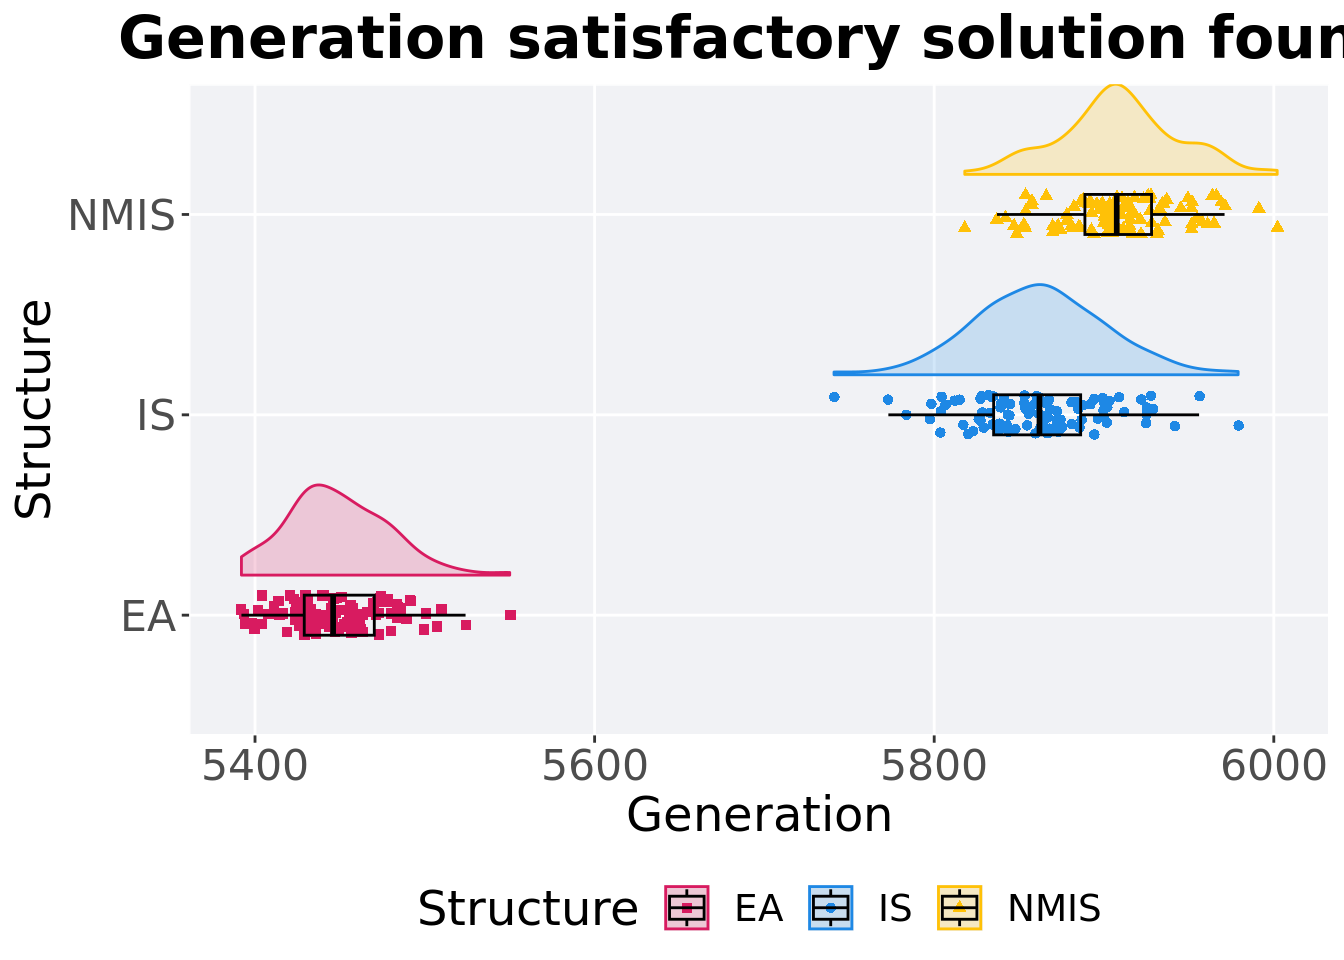
\includegraphics{demo_files/figure-latex/base-tor-exp-ssf-1.pdf}

\hypertarget{stats-26}{%
\subsection{Stats}\label{stats-26}}

Summary statistics for the first generation a satisfactory solution is found.

\begin{Shaded}
\begin{Highlighting}[]
\NormalTok{ssf =}\StringTok{ }\KeywordTok{filter}\NormalTok{(base_ssf, Diagnostic }\OperatorTok{==}\StringTok{ 'EXPLOITATION_RATE'} \OperatorTok{&}\StringTok{ `}\DataTypeTok{Selection}\CharTok{\textbackslash{}n}\DataTypeTok{Scheme}\StringTok{`} \OperatorTok{==}\StringTok{ 'TOURNAMENT'} \OperatorTok{&}\StringTok{ }\NormalTok{Generations }\OperatorTok{<}\StringTok{ }\DecValTok{60000}\NormalTok{)}
\NormalTok{ssf }\OperatorTok
\StringTok{  }\KeywordTok{group_by}\NormalTok{(Structure) }\OperatorTok
\StringTok{  }\NormalTok{dplyr}\OperatorTok{::}\KeywordTok{summarise}\NormalTok{(}
    \DataTypeTok{count =} \KeywordTok{n}\NormalTok{(),}
    \DataTypeTok{na_cnt =} \KeywordTok{sum}\NormalTok{(}\KeywordTok{is.na}\NormalTok{(Generations)),}
    \DataTypeTok{min =} \KeywordTok{min}\NormalTok{(Generations, }\DataTypeTok{na.rm =} \OtherTok{TRUE}\NormalTok{),}
    \DataTypeTok{median =} \KeywordTok{median}\NormalTok{(Generations, }\DataTypeTok{na.rm =} \OtherTok{TRUE}\NormalTok{),}
    \DataTypeTok{mean =} \KeywordTok{mean}\NormalTok{(Generations, }\DataTypeTok{na.rm =} \OtherTok{TRUE}\NormalTok{),}
    \DataTypeTok{max =} \KeywordTok{max}\NormalTok{(Generations, }\DataTypeTok{na.rm =} \OtherTok{TRUE}\NormalTok{),}
    \DataTypeTok{IQR =} \KeywordTok{IQR}\NormalTok{(Generations, }\DataTypeTok{na.rm =} \OtherTok{TRUE}\NormalTok{)}
\NormalTok{  )}
\end{Highlighting}
\end{Shaded}

\begin{verbatim}
## # A tibble: 3 x 8
##   Structure count na_cnt   min median  mean   max   IQR
##   <fct>     <int>  <int> <int>  <dbl> <dbl> <int> <dbl>
## 1 EA          100      0  5392  5446  5449.  5550  41.2
## 2 IS          100      0  5741  5862  5862.  5979  51.2
## 3 NMIS        100      0  5818  5908. 5909.  6002  39.2
\end{verbatim}

Kruskal--Wallis test provides evidence of difference among selection schemes.

\begin{Shaded}
\begin{Highlighting}[]
\KeywordTok{kruskal.test}\NormalTok{(Generations }\OperatorTok{~}\StringTok{ }\NormalTok{Structure, }\DataTypeTok{data =}\NormalTok{ ssf)}
\end{Highlighting}
\end{Shaded}

\begin{verbatim}
## 
##  Kruskal-Wallis rank sum test
## 
## data:  Generations by Structure
## Kruskal-Wallis chi-squared = 226.27, df = 2, p-value < 2.2e-16
\end{verbatim}

Results for post-hoc Wilcoxon rank-sum test with a Bonferroni correction.

\begin{Shaded}
\begin{Highlighting}[]
\KeywordTok{pairwise.wilcox.test}\NormalTok{(}\DataTypeTok{x =}\NormalTok{ ssf}\OperatorTok{$}\NormalTok{Generations, }\DataTypeTok{g =}\NormalTok{ ssf}\OperatorTok{$}\NormalTok{Structure, }\DataTypeTok{p.adjust.method =} \StringTok{"bonferroni"}\NormalTok{,}
                     \DataTypeTok{paired =} \OtherTok{FALSE}\NormalTok{, }\DataTypeTok{conf.int =} \OtherTok{FALSE}\NormalTok{, }\DataTypeTok{alternative =} \StringTok{'g'}\NormalTok{)}
\end{Highlighting}
\end{Shaded}

\begin{verbatim}
## 
##  Pairwise comparisons using Wilcoxon rank sum test with continuity correction 
## 
## data:  ssf$Generations and ssf$Structure 
## 
##      EA      IS     
## IS   < 2e-16 -      
## NMIS < 2e-16 1.1e-14
## 
## P value adjustment method: bonferroni
\end{verbatim}

\hypertarget{lexicase-selection-4}{%
\section{Lexicase selection}\label{lexicase-selection-4}}

Here we analyze how the different population structures affect standard lexicase selection on the exploitation rate diagnostic.

\hypertarget{performance-over-time-11}{%
\subsection{Performance over time}\label{performance-over-time-11}}

\begin{Shaded}
\begin{Highlighting}[]
\NormalTok{lines =}\StringTok{ }\KeywordTok{filter}\NormalTok{(base_over_time, Diagnostic }\OperatorTok{==}\StringTok{ 'EXPLOITATION_RATE'} \OperatorTok{&}\StringTok{ `}\DataTypeTok{Selection}\CharTok{\textbackslash{}n}\DataTypeTok{Scheme}\StringTok{`} \OperatorTok{==}\StringTok{ 'LEXICASE'}\NormalTok{) }\OperatorTok
\StringTok{  }\KeywordTok{group_by}\NormalTok{(Structure, Generations) }\OperatorTok
\StringTok{  }\NormalTok{dplyr}\OperatorTok{::}\KeywordTok{summarise}\NormalTok{(}
    \DataTypeTok{min =} \KeywordTok{min}\NormalTok{(pop_fit_max) }\OperatorTok{/}\StringTok{ }\NormalTok{DIMENSIONALITY,}
    \DataTypeTok{mean =} \KeywordTok{mean}\NormalTok{(pop_fit_max) }\OperatorTok{/}\StringTok{ }\NormalTok{DIMENSIONALITY,}
    \DataTypeTok{max =} \KeywordTok{max}\NormalTok{(pop_fit_max) }\OperatorTok{/}\StringTok{ }\NormalTok{DIMENSIONALITY}
\NormalTok{  )}
\KeywordTok{ggplot}\NormalTok{(lines, }\KeywordTok{aes}\NormalTok{(}\DataTypeTok{x=}\NormalTok{Generations, }\DataTypeTok{y=}\NormalTok{mean, }\DataTypeTok{group =}\NormalTok{ Structure, }\DataTypeTok{fill =}\NormalTok{ Structure, }\DataTypeTok{color =}\NormalTok{ Structure, }\DataTypeTok{shape =}\NormalTok{ Structure)) }\OperatorTok{+}
\StringTok{  }\KeywordTok{geom_ribbon}\NormalTok{(}\KeywordTok{aes}\NormalTok{(}\DataTypeTok{ymin =}\NormalTok{ min, }\DataTypeTok{ymax =}\NormalTok{ max), }\DataTypeTok{alpha =} \FloatTok{0.1}\NormalTok{) }\OperatorTok{+}
\StringTok{  }\KeywordTok{geom_line}\NormalTok{(}\DataTypeTok{size =} \FloatTok{0.5}\NormalTok{) }\OperatorTok{+}
\StringTok{  }\KeywordTok{geom_point}\NormalTok{(}\DataTypeTok{data =} \KeywordTok{filter}\NormalTok{(lines, Generations }\OperatorTok\StringTok{ }\DecValTok{2000} \OperatorTok{==}\StringTok{ }\DecValTok{0}\NormalTok{), }\DataTypeTok{size =} \FloatTok{2.5}\NormalTok{, }\DataTypeTok{stroke =} \FloatTok{2.0}\NormalTok{, }\DataTypeTok{alpha =} \FloatTok{1.0}\NormalTok{) }\OperatorTok{+}
\StringTok{  }\KeywordTok{scale_y_continuous}\NormalTok{(}
    \DataTypeTok{name=}\StringTok{"Average trait score"}\NormalTok{,}
    \DataTypeTok{limits=}\KeywordTok{c}\NormalTok{(}\OperatorTok{-}\DecValTok{1}\NormalTok{, }\DecValTok{101}\NormalTok{),}
    \DataTypeTok{breaks=}\KeywordTok{seq}\NormalTok{(}\DecValTok{0}\NormalTok{,}\DecValTok{100}\NormalTok{, }\DecValTok{20}\NormalTok{),}
    \DataTypeTok{labels=}\KeywordTok{c}\NormalTok{(}\StringTok{"0"}\NormalTok{, }\StringTok{"20"}\NormalTok{, }\StringTok{"40"}\NormalTok{, }\StringTok{"60"}\NormalTok{, }\StringTok{"80"}\NormalTok{, }\StringTok{"100"}\NormalTok{)}
\NormalTok{  ) }\OperatorTok{+}
\StringTok{  }\KeywordTok{scale_x_continuous}\NormalTok{(}
    \DataTypeTok{name=}\StringTok{"Generations"}\NormalTok{,}
    \DataTypeTok{limits=}\KeywordTok{c}\NormalTok{(}\DecValTok{0}\NormalTok{, }\DecValTok{50000}\NormalTok{),}
    \DataTypeTok{breaks=}\KeywordTok{c}\NormalTok{(}\DecValTok{0}\NormalTok{, }\DecValTok{10000}\NormalTok{, }\DecValTok{20000}\NormalTok{, }\DecValTok{30000}\NormalTok{, }\DecValTok{40000}\NormalTok{, }\DecValTok{50000}\NormalTok{),}
    \DataTypeTok{labels=}\KeywordTok{c}\NormalTok{(}\StringTok{"0e+4"}\NormalTok{, }\StringTok{"1e+4"}\NormalTok{, }\StringTok{"2e+4"}\NormalTok{, }\StringTok{"3e+4"}\NormalTok{, }\StringTok{"4e+4"}\NormalTok{, }\StringTok{"5e+4"}\NormalTok{)}

\NormalTok{  ) }\OperatorTok{+}
\StringTok{  }\KeywordTok{scale_shape_manual}\NormalTok{(}\DataTypeTok{values=}\NormalTok{SHAPE)}\OperatorTok{+}
\StringTok{  }\KeywordTok{scale_colour_manual}\NormalTok{(}\DataTypeTok{values =}\NormalTok{ cb_palette) }\OperatorTok{+}
\StringTok{  }\KeywordTok{scale_fill_manual}\NormalTok{(}\DataTypeTok{values =}\NormalTok{ cb_palette) }\OperatorTok{+}
\StringTok{  }\KeywordTok{ggtitle}\NormalTok{(}\StringTok{"Best performance over time"}\NormalTok{) }\OperatorTok{+}
\StringTok{  }\NormalTok{p_theme}
\end{Highlighting}
\end{Shaded}

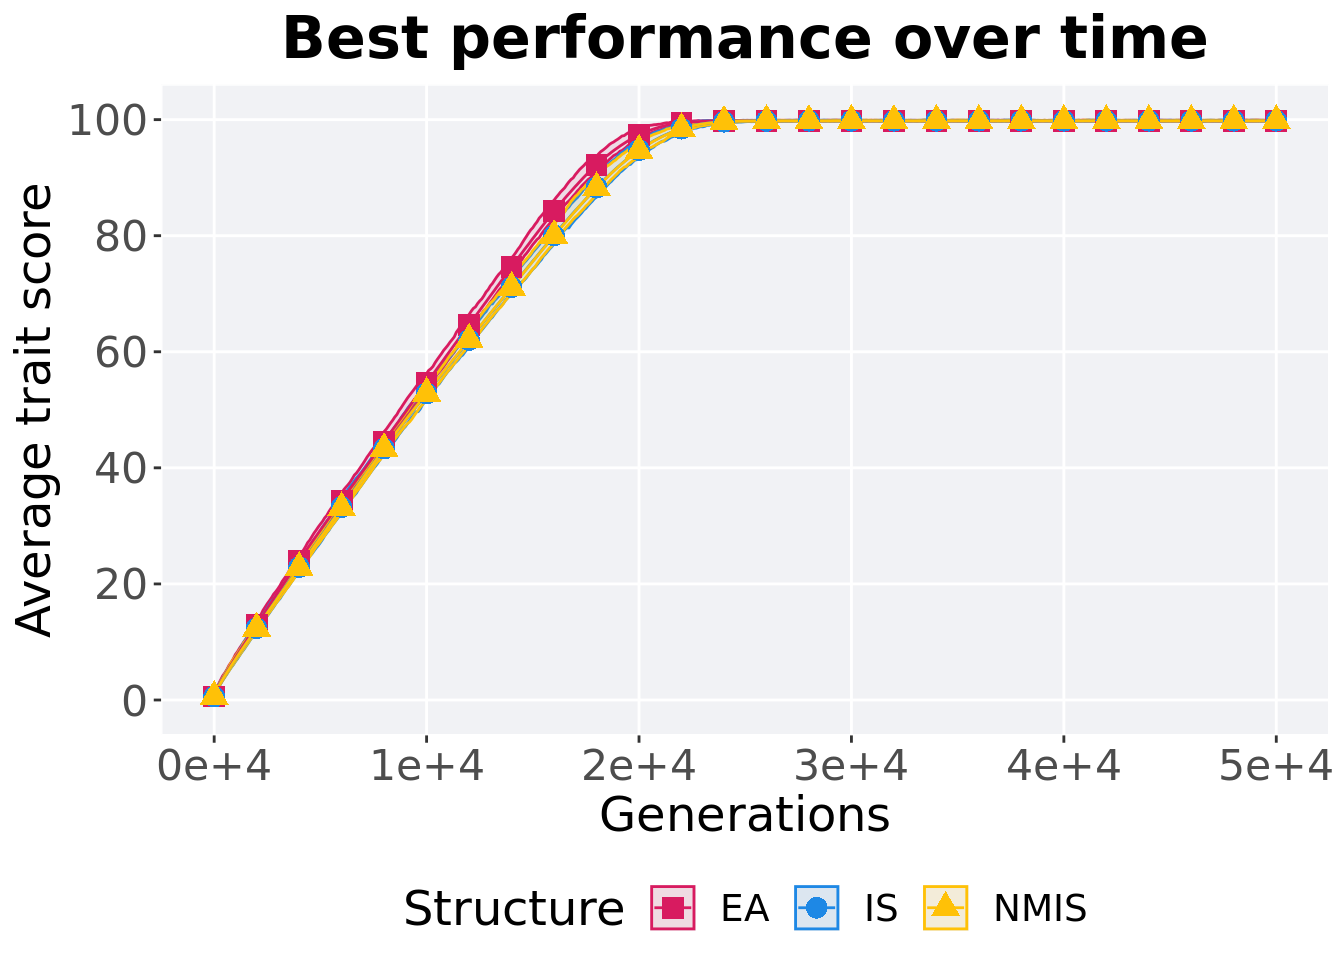
\includegraphics{demo_files/figure-latex/base-lex-exp-perf-1.pdf}

\hypertarget{generation-satisfactory-solution-found-8}{%
\subsection{Generation satisfactory solution found}\label{generation-satisfactory-solution-found-8}}

First generation a satisfactory solution is found throughout the 50,000 generations.

\begin{Shaded}
\begin{Highlighting}[]
\KeywordTok{filter}\NormalTok{(base_ssf, Diagnostic }\OperatorTok{==}\StringTok{ 'EXPLOITATION_RATE'} \OperatorTok{&}\StringTok{ `}\DataTypeTok{Selection}\CharTok{\textbackslash{}n}\DataTypeTok{Scheme}\StringTok{`} \OperatorTok{==}\StringTok{ 'LEXICASE'}\NormalTok{) }\OperatorTok
\StringTok{  }\KeywordTok{ggplot}\NormalTok{(., }\KeywordTok{aes}\NormalTok{(}\DataTypeTok{x =}\NormalTok{ Structure, }\DataTypeTok{y =}\NormalTok{ Generations , }\DataTypeTok{color =}\NormalTok{ Structure, }\DataTypeTok{fill =}\NormalTok{ Structure, }\DataTypeTok{shape =}\NormalTok{ Structure)) }\OperatorTok{+}
\StringTok{  }\KeywordTok{geom_flat_violin}\NormalTok{(}\DataTypeTok{position =} \KeywordTok{position_nudge}\NormalTok{(}\DataTypeTok{x =} \FloatTok{.2}\NormalTok{, }\DataTypeTok{y =} \DecValTok{0}\NormalTok{), }\DataTypeTok{scale =} \StringTok{'width'}\NormalTok{, }\DataTypeTok{alpha =} \FloatTok{0.2}\NormalTok{) }\OperatorTok{+}
\StringTok{  }\KeywordTok{geom_point}\NormalTok{(}\DataTypeTok{position =} \KeywordTok{position_jitter}\NormalTok{(}\DataTypeTok{width =} \FloatTok{.1}\NormalTok{), }\DataTypeTok{size =} \FloatTok{1.5}\NormalTok{, }\DataTypeTok{alpha =} \FloatTok{1.0}\NormalTok{) }\OperatorTok{+}
\StringTok{  }\KeywordTok{geom_boxplot}\NormalTok{(}\DataTypeTok{color =} \StringTok{'black'}\NormalTok{, }\DataTypeTok{width =} \FloatTok{.2}\NormalTok{, }\DataTypeTok{outlier.shape =} \OtherTok{NA}\NormalTok{, }\DataTypeTok{alpha =} \FloatTok{0.0}\NormalTok{) }\OperatorTok{+}
\StringTok{  }\KeywordTok{scale_y_continuous}\NormalTok{(}
    \DataTypeTok{name=}\StringTok{"Generation"}
\NormalTok{  ) }\OperatorTok{+}
\StringTok{  }\KeywordTok{scale_x_discrete}\NormalTok{(}
    \DataTypeTok{name=}\StringTok{"Structure"}
\NormalTok{  )}\OperatorTok{+}
\StringTok{  }\KeywordTok{scale_shape_manual}\NormalTok{(}\DataTypeTok{values=}\NormalTok{SHAPE)}\OperatorTok{+}
\StringTok{  }\KeywordTok{scale_colour_manual}\NormalTok{(}\DataTypeTok{values =}\NormalTok{ cb_palette, ) }\OperatorTok{+}
\StringTok{  }\KeywordTok{scale_fill_manual}\NormalTok{(}\DataTypeTok{values =}\NormalTok{ cb_palette) }\OperatorTok{+}
\StringTok{  }\KeywordTok{ggtitle}\NormalTok{(}\StringTok{'Generation satisfactory solution found'}\NormalTok{)}\OperatorTok{+}
\StringTok{  }\NormalTok{p_theme }\OperatorTok{+}\StringTok{ }\KeywordTok{coord_flip}\NormalTok{()}
\end{Highlighting}
\end{Shaded}

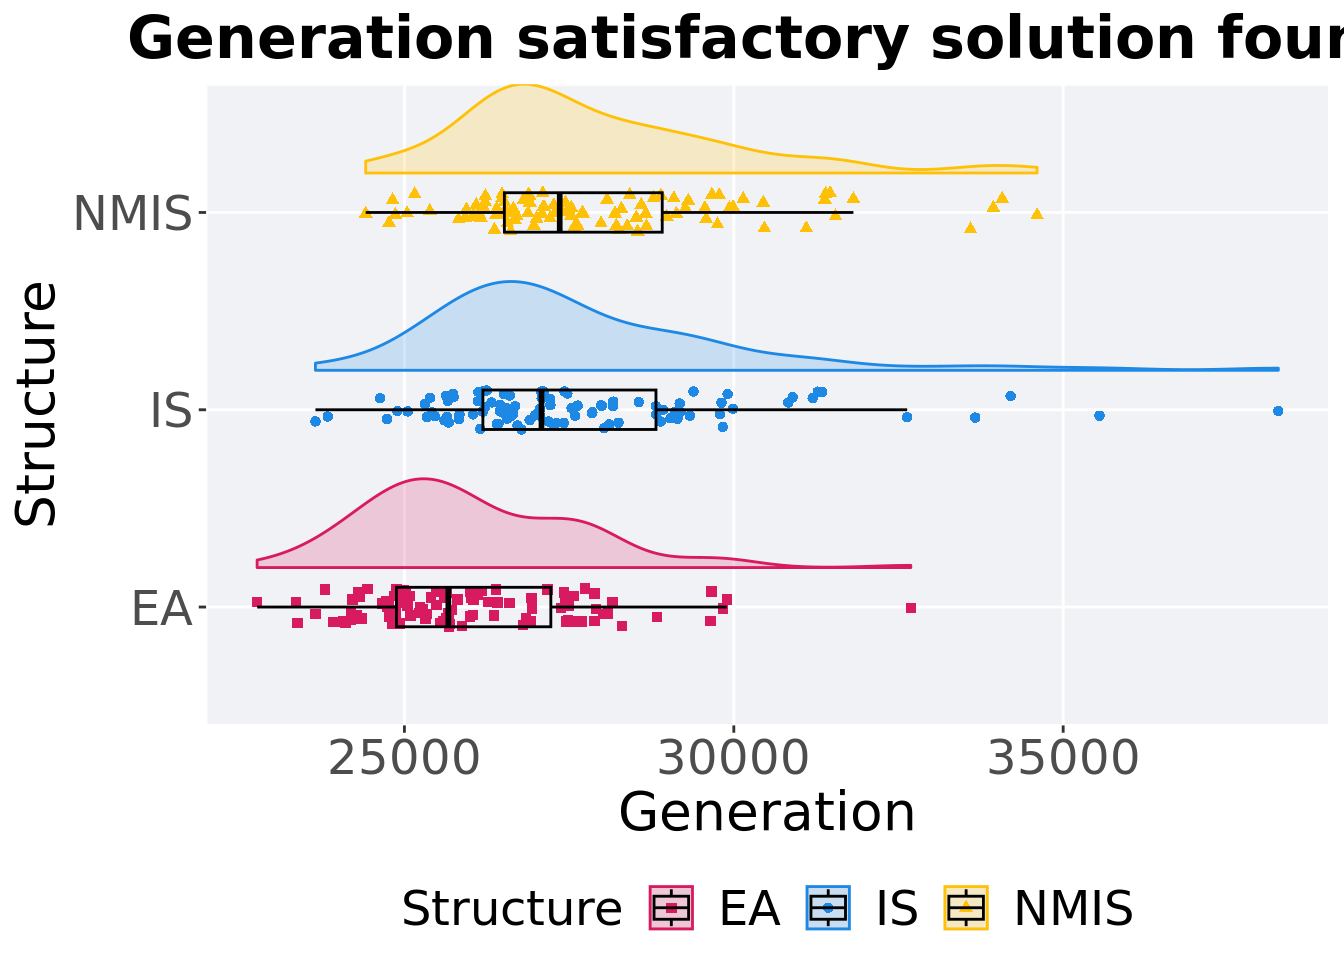
\includegraphics{demo_files/figure-latex/base-lex-exp-ssf-1.pdf}

\hypertarget{stats-27}{%
\subsection{Stats}\label{stats-27}}

Summary statistics for the first generation a satisfactory solution is found.

\begin{Shaded}
\begin{Highlighting}[]
\NormalTok{ssf =}\StringTok{ }\KeywordTok{filter}\NormalTok{(base_ssf, Diagnostic }\OperatorTok{==}\StringTok{ 'EXPLOITATION_RATE'} \OperatorTok{&}\StringTok{ `}\DataTypeTok{Selection}\CharTok{\textbackslash{}n}\DataTypeTok{Scheme}\StringTok{`} \OperatorTok{==}\StringTok{ 'LEXICASE'} \OperatorTok{&}\StringTok{ }\NormalTok{Generations }\OperatorTok{<}\StringTok{ }\DecValTok{60000}\NormalTok{)}
\NormalTok{ssf }\OperatorTok
\StringTok{  }\KeywordTok{group_by}\NormalTok{(Structure) }\OperatorTok
\StringTok{  }\NormalTok{dplyr}\OperatorTok{::}\KeywordTok{summarise}\NormalTok{(}
    \DataTypeTok{count =} \KeywordTok{n}\NormalTok{(),}
    \DataTypeTok{na_cnt =} \KeywordTok{sum}\NormalTok{(}\KeywordTok{is.na}\NormalTok{(Generations)),}
    \DataTypeTok{min =} \KeywordTok{min}\NormalTok{(Generations, }\DataTypeTok{na.rm =} \OtherTok{TRUE}\NormalTok{),}
    \DataTypeTok{median =} \KeywordTok{median}\NormalTok{(Generations, }\DataTypeTok{na.rm =} \OtherTok{TRUE}\NormalTok{),}
    \DataTypeTok{mean =} \KeywordTok{mean}\NormalTok{(Generations, }\DataTypeTok{na.rm =} \OtherTok{TRUE}\NormalTok{),}
    \DataTypeTok{max =} \KeywordTok{max}\NormalTok{(Generations, }\DataTypeTok{na.rm =} \OtherTok{TRUE}\NormalTok{),}
    \DataTypeTok{IQR =} \KeywordTok{IQR}\NormalTok{(Generations, }\DataTypeTok{na.rm =} \OtherTok{TRUE}\NormalTok{)}
\NormalTok{  )}
\end{Highlighting}
\end{Shaded}

\begin{verbatim}
## # A tibble: 3 x 8
##   Structure count na_cnt   min median   mean   max   IQR
##   <fct>     <int>  <int> <int>  <dbl>  <dbl> <int> <dbl>
## 1 EA          100      0 22764 25666. 26026. 32687 2344 
## 2 IS          100      0 23649 27080. 27635. 38266 2628.
## 3 NMIS        100      0 24412 27358. 27906. 34604 2396.
\end{verbatim}

Kruskal--Wallis test provides evidence of difference among selection schemes.

\begin{Shaded}
\begin{Highlighting}[]
\KeywordTok{kruskal.test}\NormalTok{(Generations }\OperatorTok{~}\StringTok{ }\NormalTok{Structure, }\DataTypeTok{data =}\NormalTok{ ssf)}
\end{Highlighting}
\end{Shaded}

\begin{verbatim}
## 
##  Kruskal-Wallis rank sum test
## 
## data:  Generations by Structure
## Kruskal-Wallis chi-squared = 52.814, df = 2, p-value = 3.401e-12
\end{verbatim}

Results for post-hoc Wilcoxon rank-sum test with a Bonferroni correction.

\begin{Shaded}
\begin{Highlighting}[]
\KeywordTok{pairwise.wilcox.test}\NormalTok{(}\DataTypeTok{x =}\NormalTok{ ssf}\OperatorTok{$}\NormalTok{Generations, }\DataTypeTok{g =}\NormalTok{ ssf}\OperatorTok{$}\NormalTok{Structure, }\DataTypeTok{p.adjust.method =} \StringTok{"bonferroni"}\NormalTok{,}
                     \DataTypeTok{paired =} \OtherTok{FALSE}\NormalTok{, }\DataTypeTok{conf.int =} \OtherTok{FALSE}\NormalTok{, }\DataTypeTok{alternative =} \StringTok{'g'}\NormalTok{)}
\end{Highlighting}
\end{Shaded}

\begin{verbatim}
## 
##  Pairwise comparisons using Wilcoxon rank sum test with continuity correction 
## 
## data:  ssf$Generations and ssf$Structure 
## 
##      EA      IS  
## IS   3.0e-08 -   
## NMIS 2.2e-11 0.24
## 
## P value adjustment method: bonferroni
\end{verbatim}

\hypertarget{mi500-ordered-exploitation-results}{%
\chapter{MI500: Ordered exploitation results}\label{mi500-ordered-exploitation-results}}

Here we present the results for \textbf{best performances} found by each selection scheme replicate on the ordered exploitation diagnostic with our base configurations.
Best performance found refers to the largest average trait score found in a given population.
Note that performance values fall between 0.0 and 100.0.
For our base configuration, we execute migrations every 500 generations and there are 4 islands in a ring topology.
When migrations occur, we swap two individuals (same position on each island) and guarantee that no solution can return to the same island.

\hypertarget{analysis-dependencies-5}{%
\section{Analysis dependencies}\label{analysis-dependencies-5}}

\begin{Shaded}
\begin{Highlighting}[]
\KeywordTok{library}\NormalTok{(ggplot2)}
\KeywordTok{library}\NormalTok{(cowplot)}
\KeywordTok{library}\NormalTok{(dplyr)}
\KeywordTok{library}\NormalTok{(PupillometryR)}
\end{Highlighting}
\end{Shaded}

\hypertarget{truncation-selection-5}{%
\section{Truncation selection}\label{truncation-selection-5}}

Here we analyze how the different population structures affect truncation selection (size 8) on the ordered exploitation diagnostic.

\hypertarget{performance-over-time-12}{%
\subsection{Performance over time}\label{performance-over-time-12}}

\begin{Shaded}
\begin{Highlighting}[]
\NormalTok{lines =}\StringTok{ }\KeywordTok{filter}\NormalTok{(base_over_time, Diagnostic }\OperatorTok{==}\StringTok{ 'ORDERED_EXPLOITATION'} \OperatorTok{&}\StringTok{ `}\DataTypeTok{Selection}\CharTok{\textbackslash{}n}\DataTypeTok{Scheme}\StringTok{`} \OperatorTok{==}\StringTok{ 'TRUNCATION'}\NormalTok{) }\OperatorTok
\StringTok{  }\KeywordTok{group_by}\NormalTok{(Structure, Generations) }\OperatorTok
\StringTok{  }\NormalTok{dplyr}\OperatorTok{::}\KeywordTok{summarise}\NormalTok{(}
    \DataTypeTok{min =} \KeywordTok{min}\NormalTok{(pop_fit_max) }\OperatorTok{/}\StringTok{ }\NormalTok{DIMENSIONALITY,}
    \DataTypeTok{mean =} \KeywordTok{mean}\NormalTok{(pop_fit_max) }\OperatorTok{/}\StringTok{ }\NormalTok{DIMENSIONALITY,}
    \DataTypeTok{max =} \KeywordTok{max}\NormalTok{(pop_fit_max) }\OperatorTok{/}\StringTok{ }\NormalTok{DIMENSIONALITY}
\NormalTok{  )}
\KeywordTok{ggplot}\NormalTok{(lines, }\KeywordTok{aes}\NormalTok{(}\DataTypeTok{x=}\NormalTok{Generations, }\DataTypeTok{y=}\NormalTok{mean, }\DataTypeTok{group =}\NormalTok{ Structure, }\DataTypeTok{fill =}\NormalTok{ Structure, }\DataTypeTok{color =}\NormalTok{ Structure, }\DataTypeTok{shape =}\NormalTok{ Structure)) }\OperatorTok{+}
\StringTok{  }\KeywordTok{geom_ribbon}\NormalTok{(}\KeywordTok{aes}\NormalTok{(}\DataTypeTok{ymin =}\NormalTok{ min, }\DataTypeTok{ymax =}\NormalTok{ max), }\DataTypeTok{alpha =} \FloatTok{0.1}\NormalTok{) }\OperatorTok{+}
\StringTok{  }\KeywordTok{geom_line}\NormalTok{(}\DataTypeTok{size =} \FloatTok{0.5}\NormalTok{) }\OperatorTok{+}
\StringTok{  }\KeywordTok{geom_point}\NormalTok{(}\DataTypeTok{data =} \KeywordTok{filter}\NormalTok{(lines, Generations }\OperatorTok\StringTok{ }\DecValTok{2000} \OperatorTok{==}\StringTok{ }\DecValTok{0}\NormalTok{), }\DataTypeTok{size =} \FloatTok{2.5}\NormalTok{, }\DataTypeTok{stroke =} \FloatTok{2.0}\NormalTok{, }\DataTypeTok{alpha =} \FloatTok{1.0}\NormalTok{) }\OperatorTok{+}
\StringTok{  }\KeywordTok{scale_y_continuous}\NormalTok{(}
    \DataTypeTok{name=}\StringTok{"Average trait score"}\NormalTok{,}
    \DataTypeTok{limits=}\KeywordTok{c}\NormalTok{(}\OperatorTok{-}\DecValTok{1}\NormalTok{, }\DecValTok{101}\NormalTok{),}
    \DataTypeTok{breaks=}\KeywordTok{seq}\NormalTok{(}\DecValTok{0}\NormalTok{,}\DecValTok{100}\NormalTok{, }\DecValTok{20}\NormalTok{),}
    \DataTypeTok{labels=}\KeywordTok{c}\NormalTok{(}\StringTok{"0"}\NormalTok{, }\StringTok{"20"}\NormalTok{, }\StringTok{"40"}\NormalTok{, }\StringTok{"60"}\NormalTok{, }\StringTok{"80"}\NormalTok{, }\StringTok{"100"}\NormalTok{)}
\NormalTok{  ) }\OperatorTok{+}
\StringTok{  }\KeywordTok{scale_x_continuous}\NormalTok{(}
    \DataTypeTok{name=}\StringTok{"Generations"}\NormalTok{,}
    \DataTypeTok{limits=}\KeywordTok{c}\NormalTok{(}\DecValTok{0}\NormalTok{, }\DecValTok{50000}\NormalTok{),}
    \DataTypeTok{breaks=}\KeywordTok{c}\NormalTok{(}\DecValTok{0}\NormalTok{, }\DecValTok{10000}\NormalTok{, }\DecValTok{20000}\NormalTok{, }\DecValTok{30000}\NormalTok{, }\DecValTok{40000}\NormalTok{, }\DecValTok{50000}\NormalTok{),}
    \DataTypeTok{labels=}\KeywordTok{c}\NormalTok{(}\StringTok{"0e+4"}\NormalTok{, }\StringTok{"1e+4"}\NormalTok{, }\StringTok{"2e+4"}\NormalTok{, }\StringTok{"3e+4"}\NormalTok{, }\StringTok{"4e+4"}\NormalTok{, }\StringTok{"5e+4"}\NormalTok{)}

\NormalTok{  ) }\OperatorTok{+}
\StringTok{  }\KeywordTok{scale_shape_manual}\NormalTok{(}\DataTypeTok{values=}\NormalTok{SHAPE)}\OperatorTok{+}
\StringTok{  }\KeywordTok{scale_colour_manual}\NormalTok{(}\DataTypeTok{values =}\NormalTok{ cb_palette) }\OperatorTok{+}
\StringTok{  }\KeywordTok{scale_fill_manual}\NormalTok{(}\DataTypeTok{values =}\NormalTok{ cb_palette) }\OperatorTok{+}
\StringTok{  }\KeywordTok{ggtitle}\NormalTok{(}\StringTok{"Performance over time"}\NormalTok{) }\OperatorTok{+}
\StringTok{  }\NormalTok{p_theme}
\end{Highlighting}
\end{Shaded}

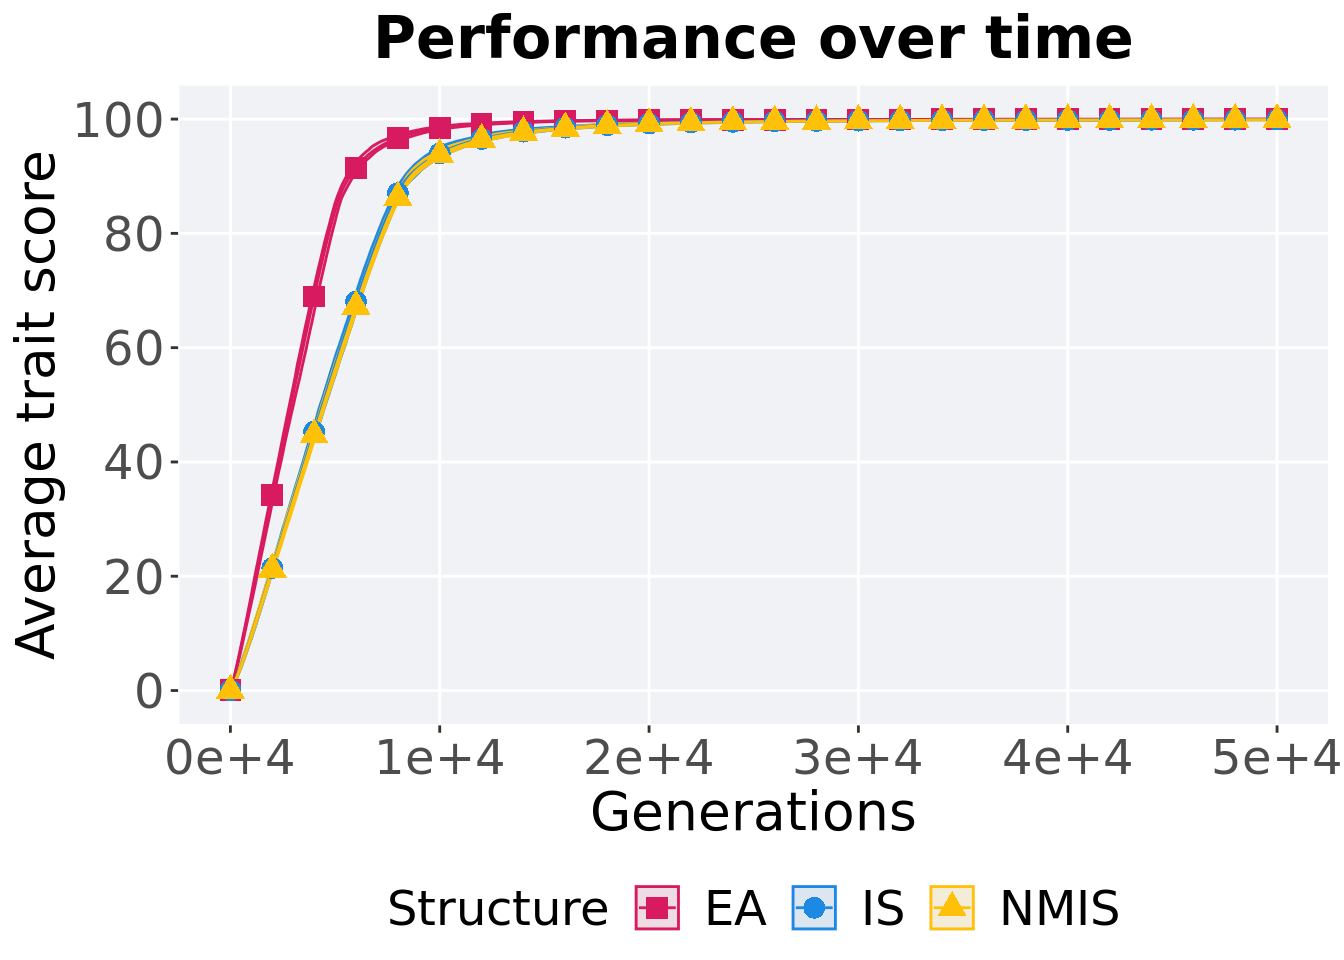
\includegraphics{demo_files/figure-latex/base-tru-ord-perf-1.pdf}

\hypertarget{generation-satisfactory-solution-found-9}{%
\subsection{Generation satisfactory solution found}\label{generation-satisfactory-solution-found-9}}

First generation a satisfactory solution is found throughout the 50,000 generations.

\begin{Shaded}
\begin{Highlighting}[]
\KeywordTok{filter}\NormalTok{(base_ssf, Diagnostic }\OperatorTok{==}\StringTok{ 'ORDERED_EXPLOITATION'} \OperatorTok{&}\StringTok{ `}\DataTypeTok{Selection}\CharTok{\textbackslash{}n}\DataTypeTok{Scheme}\StringTok{`} \OperatorTok{==}\StringTok{ 'TRUNCATION'}\NormalTok{) }\OperatorTok
\StringTok{  }\KeywordTok{ggplot}\NormalTok{(., }\KeywordTok{aes}\NormalTok{(}\DataTypeTok{x =}\NormalTok{ Structure, }\DataTypeTok{y =}\NormalTok{ Generations , }\DataTypeTok{color =}\NormalTok{ Structure, }\DataTypeTok{fill =}\NormalTok{ Structure, }\DataTypeTok{shape =}\NormalTok{ Structure)) }\OperatorTok{+}
\StringTok{  }\KeywordTok{geom_flat_violin}\NormalTok{(}\DataTypeTok{position =} \KeywordTok{position_nudge}\NormalTok{(}\DataTypeTok{x =} \FloatTok{.2}\NormalTok{, }\DataTypeTok{y =} \DecValTok{0}\NormalTok{), }\DataTypeTok{scale =} \StringTok{'width'}\NormalTok{, }\DataTypeTok{alpha =} \FloatTok{0.2}\NormalTok{) }\OperatorTok{+}
\StringTok{  }\KeywordTok{geom_point}\NormalTok{(}\DataTypeTok{position =} \KeywordTok{position_jitter}\NormalTok{(}\DataTypeTok{width =} \FloatTok{.1}\NormalTok{), }\DataTypeTok{size =} \FloatTok{1.5}\NormalTok{, }\DataTypeTok{alpha =} \FloatTok{1.0}\NormalTok{) }\OperatorTok{+}
\StringTok{  }\KeywordTok{geom_boxplot}\NormalTok{(}\DataTypeTok{color =} \StringTok{'black'}\NormalTok{, }\DataTypeTok{width =} \FloatTok{.2}\NormalTok{, }\DataTypeTok{outlier.shape =} \OtherTok{NA}\NormalTok{, }\DataTypeTok{alpha =} \FloatTok{0.0}\NormalTok{) }\OperatorTok{+}
\StringTok{  }\KeywordTok{scale_y_continuous}\NormalTok{(}
    \DataTypeTok{name=}\StringTok{"Generation"}
\NormalTok{  ) }\OperatorTok{+}
\StringTok{  }\KeywordTok{scale_x_discrete}\NormalTok{(}
    \DataTypeTok{name=}\StringTok{"Structure"}
\NormalTok{  )}\OperatorTok{+}
\StringTok{  }\KeywordTok{scale_shape_manual}\NormalTok{(}\DataTypeTok{values=}\NormalTok{SHAPE)}\OperatorTok{+}
\StringTok{  }\KeywordTok{scale_colour_manual}\NormalTok{(}\DataTypeTok{values =}\NormalTok{ cb_palette, ) }\OperatorTok{+}
\StringTok{  }\KeywordTok{scale_fill_manual}\NormalTok{(}\DataTypeTok{values =}\NormalTok{ cb_palette) }\OperatorTok{+}
\StringTok{  }\KeywordTok{ggtitle}\NormalTok{(}\StringTok{'Generation satisfactory solution found'}\NormalTok{)}\OperatorTok{+}
\StringTok{  }\NormalTok{p_theme }\OperatorTok{+}\StringTok{ }\KeywordTok{coord_flip}\NormalTok{()}
\end{Highlighting}
\end{Shaded}

\includegraphics{demo_files/figure-latex/base-tru-ord-ssf-1.pdf}

\hypertarget{stats-28}{%
\subsubsection{Stats}\label{stats-28}}

Summary statistics for the first generation a satisfactory solution is found.

\begin{Shaded}
\begin{Highlighting}[]
\NormalTok{ssf =}\StringTok{ }\KeywordTok{filter}\NormalTok{(base_ssf, Diagnostic }\OperatorTok{==}\StringTok{ 'ORDERED_EXPLOITATION'} \OperatorTok{&}\StringTok{ `}\DataTypeTok{Selection}\CharTok{\textbackslash{}n}\DataTypeTok{Scheme}\StringTok{`} \OperatorTok{==}\StringTok{ 'TRUNCATION'} \OperatorTok{&}\StringTok{ }\NormalTok{Generations }\OperatorTok{<}\StringTok{ }\DecValTok{60000}\NormalTok{)}
\NormalTok{ssf }\OperatorTok
\StringTok{  }\KeywordTok{group_by}\NormalTok{(Structure) }\OperatorTok
\StringTok{  }\NormalTok{dplyr}\OperatorTok{::}\KeywordTok{summarise}\NormalTok{(}
    \DataTypeTok{count =} \KeywordTok{n}\NormalTok{(),}
    \DataTypeTok{na_cnt =} \KeywordTok{sum}\NormalTok{(}\KeywordTok{is.na}\NormalTok{(Generations)),}
    \DataTypeTok{min =} \KeywordTok{min}\NormalTok{(Generations, }\DataTypeTok{na.rm =} \OtherTok{TRUE}\NormalTok{),}
    \DataTypeTok{median =} \KeywordTok{median}\NormalTok{(Generations, }\DataTypeTok{na.rm =} \OtherTok{TRUE}\NormalTok{),}
    \DataTypeTok{mean =} \KeywordTok{mean}\NormalTok{(Generations, }\DataTypeTok{na.rm =} \OtherTok{TRUE}\NormalTok{),}
    \DataTypeTok{max =} \KeywordTok{max}\NormalTok{(Generations, }\DataTypeTok{na.rm =} \OtherTok{TRUE}\NormalTok{),}
    \DataTypeTok{IQR =} \KeywordTok{IQR}\NormalTok{(Generations, }\DataTypeTok{na.rm =} \OtherTok{TRUE}\NormalTok{)}
\NormalTok{  )}
\end{Highlighting}
\end{Shaded}

\begin{verbatim}
## # A tibble: 3 x 8
##   Structure count na_cnt   min median   mean   max   IQR
##   <fct>     <int>  <int> <int>  <dbl>  <dbl> <int> <dbl>
## 1 EA          100      0 14684 15546  15554. 16254  492.
## 2 IS          100      0 24669 26780. 26767. 28518 1318.
## 3 NMIS        100      0 26330 27939  27888. 29654  825.
\end{verbatim}

Kruskal--Wallis test provides evidence of difference among selection schemes.

\begin{Shaded}
\begin{Highlighting}[]
\KeywordTok{kruskal.test}\NormalTok{(Generations }\OperatorTok{~}\StringTok{ }\NormalTok{Structure, }\DataTypeTok{data =}\NormalTok{ ssf)}
\end{Highlighting}
\end{Shaded}

\begin{verbatim}
## 
##  Kruskal-Wallis rank sum test
## 
## data:  Generations by Structure
## Kruskal-Wallis chi-squared = 231.88, df = 2, p-value < 2.2e-16
\end{verbatim}

Results for post-hoc Wilcoxon rank-sum test with a Bonferroni correction.

\begin{Shaded}
\begin{Highlighting}[]
\KeywordTok{pairwise.wilcox.test}\NormalTok{(}\DataTypeTok{x =}\NormalTok{ ssf}\OperatorTok{$}\NormalTok{Generations, }\DataTypeTok{g =}\NormalTok{ ssf}\OperatorTok{$}\NormalTok{Structure, }\DataTypeTok{p.adjust.method =} \StringTok{"bonferroni"}\NormalTok{,}
                     \DataTypeTok{paired =} \OtherTok{FALSE}\NormalTok{, }\DataTypeTok{conf.int =} \OtherTok{FALSE}\NormalTok{, }\DataTypeTok{alternative =} \StringTok{'g'}\NormalTok{)}
\end{Highlighting}
\end{Shaded}

\begin{verbatim}
## 
##  Pairwise comparisons using Wilcoxon rank sum test with continuity correction 
## 
## data:  ssf$Generations and ssf$Structure 
## 
##      EA     IS    
## IS   <2e-16 -     
## NMIS <2e-16 <2e-16
## 
## P value adjustment method: bonferroni
\end{verbatim}

\hypertarget{tournament-selection-5}{%
\section{Tournament selection}\label{tournament-selection-5}}

Here we analyze how the different population structures affect tournament selection (size 8) on the ordered exploitation diagnostic.

\hypertarget{performance-over-time-13}{%
\subsection{Performance over time}\label{performance-over-time-13}}

\begin{Shaded}
\begin{Highlighting}[]
\NormalTok{lines =}\StringTok{ }\KeywordTok{filter}\NormalTok{(base_over_time, Diagnostic }\OperatorTok{==}\StringTok{ 'ORDERED_EXPLOITATION'} \OperatorTok{&}\StringTok{ `}\DataTypeTok{Selection}\CharTok{\textbackslash{}n}\DataTypeTok{Scheme}\StringTok{`} \OperatorTok{==}\StringTok{ 'TOURNAMENT'}\NormalTok{) }\OperatorTok
\StringTok{  }\KeywordTok{group_by}\NormalTok{(Structure, Generations) }\OperatorTok
\StringTok{  }\NormalTok{dplyr}\OperatorTok{::}\KeywordTok{summarise}\NormalTok{(}
    \DataTypeTok{min =} \KeywordTok{min}\NormalTok{(pop_fit_max) }\OperatorTok{/}\StringTok{ }\NormalTok{DIMENSIONALITY,}
    \DataTypeTok{mean =} \KeywordTok{mean}\NormalTok{(pop_fit_max) }\OperatorTok{/}\StringTok{ }\NormalTok{DIMENSIONALITY,}
    \DataTypeTok{max =} \KeywordTok{max}\NormalTok{(pop_fit_max) }\OperatorTok{/}\StringTok{ }\NormalTok{DIMENSIONALITY}
\NormalTok{  )}
\KeywordTok{ggplot}\NormalTok{(lines, }\KeywordTok{aes}\NormalTok{(}\DataTypeTok{x=}\NormalTok{Generations, }\DataTypeTok{y=}\NormalTok{mean, }\DataTypeTok{group =}\NormalTok{ Structure, }\DataTypeTok{fill =}\NormalTok{ Structure, }\DataTypeTok{color =}\NormalTok{ Structure, }\DataTypeTok{shape =}\NormalTok{ Structure)) }\OperatorTok{+}
\StringTok{  }\KeywordTok{geom_ribbon}\NormalTok{(}\KeywordTok{aes}\NormalTok{(}\DataTypeTok{ymin =}\NormalTok{ min, }\DataTypeTok{ymax =}\NormalTok{ max), }\DataTypeTok{alpha =} \FloatTok{0.1}\NormalTok{) }\OperatorTok{+}
\StringTok{  }\KeywordTok{geom_line}\NormalTok{(}\DataTypeTok{size =} \FloatTok{0.5}\NormalTok{) }\OperatorTok{+}
\StringTok{  }\KeywordTok{geom_point}\NormalTok{(}\DataTypeTok{data =} \KeywordTok{filter}\NormalTok{(lines, Generations }\OperatorTok\StringTok{ }\DecValTok{2000} \OperatorTok{==}\StringTok{ }\DecValTok{0}\NormalTok{), }\DataTypeTok{size =} \FloatTok{2.5}\NormalTok{, }\DataTypeTok{stroke =} \FloatTok{2.0}\NormalTok{, }\DataTypeTok{alpha =} \FloatTok{1.0}\NormalTok{) }\OperatorTok{+}
\StringTok{  }\KeywordTok{scale_y_continuous}\NormalTok{(}
    \DataTypeTok{name=}\StringTok{"Average trait score"}\NormalTok{,}
    \DataTypeTok{limits=}\KeywordTok{c}\NormalTok{(}\OperatorTok{-}\DecValTok{1}\NormalTok{, }\DecValTok{101}\NormalTok{),}
    \DataTypeTok{breaks=}\KeywordTok{seq}\NormalTok{(}\DecValTok{0}\NormalTok{,}\DecValTok{100}\NormalTok{, }\DecValTok{20}\NormalTok{),}
    \DataTypeTok{labels=}\KeywordTok{c}\NormalTok{(}\StringTok{"0"}\NormalTok{, }\StringTok{"20"}\NormalTok{, }\StringTok{"40"}\NormalTok{, }\StringTok{"60"}\NormalTok{, }\StringTok{"80"}\NormalTok{, }\StringTok{"100"}\NormalTok{)}
\NormalTok{  ) }\OperatorTok{+}
\StringTok{  }\KeywordTok{scale_x_continuous}\NormalTok{(}
    \DataTypeTok{name=}\StringTok{"Generations"}\NormalTok{,}
    \DataTypeTok{limits=}\KeywordTok{c}\NormalTok{(}\DecValTok{0}\NormalTok{, }\DecValTok{50000}\NormalTok{),}
    \DataTypeTok{breaks=}\KeywordTok{c}\NormalTok{(}\DecValTok{0}\NormalTok{, }\DecValTok{10000}\NormalTok{, }\DecValTok{20000}\NormalTok{, }\DecValTok{30000}\NormalTok{, }\DecValTok{40000}\NormalTok{, }\DecValTok{50000}\NormalTok{),}
    \DataTypeTok{labels=}\KeywordTok{c}\NormalTok{(}\StringTok{"0e+4"}\NormalTok{, }\StringTok{"1e+4"}\NormalTok{, }\StringTok{"2e+4"}\NormalTok{, }\StringTok{"3e+4"}\NormalTok{, }\StringTok{"4e+4"}\NormalTok{, }\StringTok{"5e+4"}\NormalTok{)}

\NormalTok{  ) }\OperatorTok{+}
\StringTok{  }\KeywordTok{scale_shape_manual}\NormalTok{(}\DataTypeTok{values=}\NormalTok{SHAPE)}\OperatorTok{+}
\StringTok{  }\KeywordTok{scale_colour_manual}\NormalTok{(}\DataTypeTok{values =}\NormalTok{ cb_palette) }\OperatorTok{+}
\StringTok{  }\KeywordTok{scale_fill_manual}\NormalTok{(}\DataTypeTok{values =}\NormalTok{ cb_palette) }\OperatorTok{+}
\StringTok{  }\KeywordTok{ggtitle}\NormalTok{(}\StringTok{"Performance over time"}\NormalTok{) }\OperatorTok{+}
\StringTok{  }\NormalTok{p_theme}
\end{Highlighting}
\end{Shaded}

\includegraphics{demo_files/figure-latex/base-tor-ord-perf-1.pdf}

\hypertarget{generation-satisfactory-solution-found-10}{%
\subsection{Generation satisfactory solution found}\label{generation-satisfactory-solution-found-10}}

First generation a satisfactory solution is found throughout the 50,000 generations.

\begin{Shaded}
\begin{Highlighting}[]
\KeywordTok{filter}\NormalTok{(base_ssf, Diagnostic }\OperatorTok{==}\StringTok{ 'ORDERED_EXPLOITATION'} \OperatorTok{&}\StringTok{ `}\DataTypeTok{Selection}\CharTok{\textbackslash{}n}\DataTypeTok{Scheme}\StringTok{`} \OperatorTok{==}\StringTok{ 'TOURNAMENT'}\NormalTok{) }\OperatorTok
\StringTok{  }\KeywordTok{ggplot}\NormalTok{(., }\KeywordTok{aes}\NormalTok{(}\DataTypeTok{x =}\NormalTok{ Structure, }\DataTypeTok{y =}\NormalTok{ Generations , }\DataTypeTok{color =}\NormalTok{ Structure, }\DataTypeTok{fill =}\NormalTok{ Structure, }\DataTypeTok{shape =}\NormalTok{ Structure)) }\OperatorTok{+}
\StringTok{  }\KeywordTok{geom_flat_violin}\NormalTok{(}\DataTypeTok{position =} \KeywordTok{position_nudge}\NormalTok{(}\DataTypeTok{x =} \FloatTok{.2}\NormalTok{, }\DataTypeTok{y =} \DecValTok{0}\NormalTok{), }\DataTypeTok{scale =} \StringTok{'width'}\NormalTok{, }\DataTypeTok{alpha =} \FloatTok{0.2}\NormalTok{) }\OperatorTok{+}
\StringTok{  }\KeywordTok{geom_point}\NormalTok{(}\DataTypeTok{position =} \KeywordTok{position_jitter}\NormalTok{(}\DataTypeTok{width =} \FloatTok{.1}\NormalTok{), }\DataTypeTok{size =} \FloatTok{1.5}\NormalTok{, }\DataTypeTok{alpha =} \FloatTok{1.0}\NormalTok{) }\OperatorTok{+}
\StringTok{  }\KeywordTok{geom_boxplot}\NormalTok{(}\DataTypeTok{color =} \StringTok{'black'}\NormalTok{, }\DataTypeTok{width =} \FloatTok{.2}\NormalTok{, }\DataTypeTok{outlier.shape =} \OtherTok{NA}\NormalTok{, }\DataTypeTok{alpha =} \FloatTok{0.0}\NormalTok{) }\OperatorTok{+}
\StringTok{  }\KeywordTok{scale_y_continuous}\NormalTok{(}
    \DataTypeTok{name=}\StringTok{"Generation"}
\NormalTok{  ) }\OperatorTok{+}
\StringTok{  }\KeywordTok{scale_x_discrete}\NormalTok{(}
    \DataTypeTok{name=}\StringTok{"Structure"}
\NormalTok{  )}\OperatorTok{+}
\StringTok{  }\KeywordTok{scale_shape_manual}\NormalTok{(}\DataTypeTok{values=}\NormalTok{SHAPE)}\OperatorTok{+}
\StringTok{  }\KeywordTok{scale_colour_manual}\NormalTok{(}\DataTypeTok{values =}\NormalTok{ cb_palette, ) }\OperatorTok{+}
\StringTok{  }\KeywordTok{scale_fill_manual}\NormalTok{(}\DataTypeTok{values =}\NormalTok{ cb_palette) }\OperatorTok{+}
\StringTok{  }\KeywordTok{ggtitle}\NormalTok{(}\StringTok{'Generation satisfactory solution found'}\NormalTok{)}\OperatorTok{+}
\StringTok{  }\NormalTok{p_theme }\OperatorTok{+}\StringTok{ }\KeywordTok{coord_flip}\NormalTok{()}
\end{Highlighting}
\end{Shaded}

\includegraphics{demo_files/figure-latex/base-tor-ord-ssf-1.pdf}

\hypertarget{stats-29}{%
\subsubsection{Stats}\label{stats-29}}

Summary statistics for the first generation a satisfactory solution is found.

\begin{Shaded}
\begin{Highlighting}[]
\NormalTok{ssf =}\StringTok{ }\KeywordTok{filter}\NormalTok{(base_ssf, Diagnostic }\OperatorTok{==}\StringTok{ 'ORDERED_EXPLOITATION'} \OperatorTok{&}\StringTok{ `}\DataTypeTok{Selection}\CharTok{\textbackslash{}n}\DataTypeTok{Scheme}\StringTok{`} \OperatorTok{==}\StringTok{ 'TOURNAMENT'} \OperatorTok{&}\StringTok{ }\NormalTok{Generations }\OperatorTok{<}\StringTok{ }\DecValTok{60000}\NormalTok{)}
\NormalTok{ssf }\OperatorTok
\StringTok{  }\KeywordTok{group_by}\NormalTok{(Structure) }\OperatorTok
\StringTok{  }\NormalTok{dplyr}\OperatorTok{::}\KeywordTok{summarise}\NormalTok{(}
    \DataTypeTok{count =} \KeywordTok{n}\NormalTok{(),}
    \DataTypeTok{na_cnt =} \KeywordTok{sum}\NormalTok{(}\KeywordTok{is.na}\NormalTok{(Generations)),}
    \DataTypeTok{min =} \KeywordTok{min}\NormalTok{(Generations, }\DataTypeTok{na.rm =} \OtherTok{TRUE}\NormalTok{),}
    \DataTypeTok{median =} \KeywordTok{median}\NormalTok{(Generations, }\DataTypeTok{na.rm =} \OtherTok{TRUE}\NormalTok{),}
    \DataTypeTok{mean =} \KeywordTok{mean}\NormalTok{(Generations, }\DataTypeTok{na.rm =} \OtherTok{TRUE}\NormalTok{),}
    \DataTypeTok{max =} \KeywordTok{max}\NormalTok{(Generations, }\DataTypeTok{na.rm =} \OtherTok{TRUE}\NormalTok{),}
    \DataTypeTok{IQR =} \KeywordTok{IQR}\NormalTok{(Generations, }\DataTypeTok{na.rm =} \OtherTok{TRUE}\NormalTok{)}
\NormalTok{  )}
\end{Highlighting}
\end{Shaded}

\begin{verbatim}
## # A tibble: 3 x 8
##   Structure count na_cnt   min median   mean   max   IQR
##   <fct>     <int>  <int> <int>  <dbl>  <dbl> <int> <dbl>
## 1 EA          100      0 25242 27228. 27172. 28742  921.
## 2 IS          100      0 30589 34356. 34349. 36461 1564.
## 3 NMIS        100      0 33412 35764  35692. 37306 1213
\end{verbatim}

Kruskal--Wallis test provides evidence of difference among selection schemes.

\begin{Shaded}
\begin{Highlighting}[]
\KeywordTok{kruskal.test}\NormalTok{(Generations }\OperatorTok{~}\StringTok{ }\NormalTok{Structure, }\DataTypeTok{data =}\NormalTok{ ssf)}
\end{Highlighting}
\end{Shaded}

\begin{verbatim}
## 
##  Kruskal-Wallis rank sum test
## 
## data:  Generations by Structure
## Kruskal-Wallis chi-squared = 229.49, df = 2, p-value < 2.2e-16
\end{verbatim}

Results for post-hoc Wilcoxon rank-sum test with a Bonferroni correction.

\begin{Shaded}
\begin{Highlighting}[]
\KeywordTok{pairwise.wilcox.test}\NormalTok{(}\DataTypeTok{x =}\NormalTok{ ssf}\OperatorTok{$}\NormalTok{Generations, }\DataTypeTok{g =}\NormalTok{ ssf}\OperatorTok{$}\NormalTok{Structure, }\DataTypeTok{p.adjust.method =} \StringTok{"bonferroni"}\NormalTok{,}
                     \DataTypeTok{paired =} \OtherTok{FALSE}\NormalTok{, }\DataTypeTok{conf.int =} \OtherTok{FALSE}\NormalTok{, }\DataTypeTok{alternative =} \StringTok{'g'}\NormalTok{)}
\end{Highlighting}
\end{Shaded}

\begin{verbatim}
## 
##  Pairwise comparisons using Wilcoxon rank sum test with continuity correction 
## 
## data:  ssf$Generations and ssf$Structure 
## 
##      EA      IS     
## IS   < 2e-16 -      
## NMIS < 2e-16 2.8e-16
## 
## P value adjustment method: bonferroni
\end{verbatim}

\hypertarget{lexicase-selection-5}{%
\section{Lexicase selection}\label{lexicase-selection-5}}

Here we analyze how the different population structures affect standard lexicase selection on the ordered exploitation diagnostic.

\hypertarget{performance-over-time-14}{%
\subsection{Performance over time}\label{performance-over-time-14}}

\begin{Shaded}
\begin{Highlighting}[]
\NormalTok{lines =}\StringTok{ }\KeywordTok{filter}\NormalTok{(base_over_time, Diagnostic }\OperatorTok{==}\StringTok{ 'ORDERED_EXPLOITATION'} \OperatorTok{&}\StringTok{ `}\DataTypeTok{Selection}\CharTok{\textbackslash{}n}\DataTypeTok{Scheme}\StringTok{`} \OperatorTok{==}\StringTok{ 'LEXICASE'}\NormalTok{) }\OperatorTok
\StringTok{  }\KeywordTok{group_by}\NormalTok{(Structure, Generations) }\OperatorTok
\StringTok{  }\NormalTok{dplyr}\OperatorTok{::}\KeywordTok{summarise}\NormalTok{(}
    \DataTypeTok{min =} \KeywordTok{min}\NormalTok{(pop_fit_max) }\OperatorTok{/}\StringTok{ }\NormalTok{DIMENSIONALITY,}
    \DataTypeTok{mean =} \KeywordTok{mean}\NormalTok{(pop_fit_max) }\OperatorTok{/}\StringTok{ }\NormalTok{DIMENSIONALITY,}
    \DataTypeTok{max =} \KeywordTok{max}\NormalTok{(pop_fit_max) }\OperatorTok{/}\StringTok{ }\NormalTok{DIMENSIONALITY}
\NormalTok{  )}
\KeywordTok{ggplot}\NormalTok{(lines, }\KeywordTok{aes}\NormalTok{(}\DataTypeTok{x=}\NormalTok{Generations, }\DataTypeTok{y=}\NormalTok{mean, }\DataTypeTok{group =}\NormalTok{ Structure, }\DataTypeTok{fill =}\NormalTok{ Structure, }\DataTypeTok{color =}\NormalTok{ Structure, }\DataTypeTok{shape =}\NormalTok{ Structure)) }\OperatorTok{+}
\StringTok{  }\KeywordTok{geom_ribbon}\NormalTok{(}\KeywordTok{aes}\NormalTok{(}\DataTypeTok{ymin =}\NormalTok{ min, }\DataTypeTok{ymax =}\NormalTok{ max), }\DataTypeTok{alpha =} \FloatTok{0.1}\NormalTok{) }\OperatorTok{+}
\StringTok{  }\KeywordTok{geom_line}\NormalTok{(}\DataTypeTok{size =} \FloatTok{0.5}\NormalTok{) }\OperatorTok{+}
\StringTok{  }\KeywordTok{geom_point}\NormalTok{(}\DataTypeTok{data =} \KeywordTok{filter}\NormalTok{(lines, Generations }\OperatorTok\StringTok{ }\DecValTok{2000} \OperatorTok{==}\StringTok{ }\DecValTok{0}\NormalTok{), }\DataTypeTok{size =} \FloatTok{2.5}\NormalTok{, }\DataTypeTok{stroke =} \FloatTok{2.0}\NormalTok{, }\DataTypeTok{alpha =} \FloatTok{1.0}\NormalTok{) }\OperatorTok{+}
\StringTok{  }\KeywordTok{scale_y_continuous}\NormalTok{(}
    \DataTypeTok{name=}\StringTok{"Average trait score"}\NormalTok{,}
    \DataTypeTok{limits=}\KeywordTok{c}\NormalTok{(}\OperatorTok{-}\DecValTok{1}\NormalTok{, }\DecValTok{101}\NormalTok{),}
    \DataTypeTok{breaks=}\KeywordTok{seq}\NormalTok{(}\DecValTok{0}\NormalTok{,}\DecValTok{100}\NormalTok{, }\DecValTok{20}\NormalTok{),}
    \DataTypeTok{labels=}\KeywordTok{c}\NormalTok{(}\StringTok{"0"}\NormalTok{, }\StringTok{"20"}\NormalTok{, }\StringTok{"40"}\NormalTok{, }\StringTok{"60"}\NormalTok{, }\StringTok{"80"}\NormalTok{, }\StringTok{"100"}\NormalTok{)}
\NormalTok{  ) }\OperatorTok{+}
\StringTok{  }\KeywordTok{scale_x_continuous}\NormalTok{(}
    \DataTypeTok{name=}\StringTok{"Generations"}\NormalTok{,}
    \DataTypeTok{limits=}\KeywordTok{c}\NormalTok{(}\DecValTok{0}\NormalTok{, }\DecValTok{50000}\NormalTok{),}
    \DataTypeTok{breaks=}\KeywordTok{c}\NormalTok{(}\DecValTok{0}\NormalTok{, }\DecValTok{10000}\NormalTok{, }\DecValTok{20000}\NormalTok{, }\DecValTok{30000}\NormalTok{, }\DecValTok{40000}\NormalTok{, }\DecValTok{50000}\NormalTok{),}
    \DataTypeTok{labels=}\KeywordTok{c}\NormalTok{(}\StringTok{"0e+4"}\NormalTok{, }\StringTok{"1e+4"}\NormalTok{, }\StringTok{"2e+4"}\NormalTok{, }\StringTok{"3e+4"}\NormalTok{, }\StringTok{"4e+4"}\NormalTok{, }\StringTok{"5e+4"}\NormalTok{)}

\NormalTok{  ) }\OperatorTok{+}
\StringTok{  }\KeywordTok{scale_shape_manual}\NormalTok{(}\DataTypeTok{values=}\NormalTok{SHAPE)}\OperatorTok{+}
\StringTok{  }\KeywordTok{scale_colour_manual}\NormalTok{(}\DataTypeTok{values =}\NormalTok{ cb_palette) }\OperatorTok{+}
\StringTok{  }\KeywordTok{scale_fill_manual}\NormalTok{(}\DataTypeTok{values =}\NormalTok{ cb_palette) }\OperatorTok{+}
\StringTok{  }\KeywordTok{ggtitle}\NormalTok{(}\StringTok{"Performance over time"}\NormalTok{) }\OperatorTok{+}
\StringTok{  }\NormalTok{p_theme}
\end{Highlighting}
\end{Shaded}

\includegraphics{demo_files/figure-latex/base-lex-ord-perf-1.pdf}

\hypertarget{best-performance-3}{%
\subsection{Best performance}\label{best-performance-3}}

First generation a satisfactory solution is found throughout the 50,000 generations.

\begin{Shaded}
\begin{Highlighting}[]
\KeywordTok{filter}\NormalTok{(base_best, Diagnostic }\OperatorTok{==}\StringTok{ 'ORDERED_EXPLOITATION'} \OperatorTok{&}\StringTok{ `}\DataTypeTok{Selection}\CharTok{\textbackslash{}n}\DataTypeTok{Scheme}\StringTok{`} \OperatorTok{==}\StringTok{ 'LEXICASE'} \OperatorTok{&}\StringTok{ }\NormalTok{VAR }\OperatorTok{==}\StringTok{ 'pop_fit_max'}\NormalTok{) }\OperatorTok
\StringTok{  }\KeywordTok{ggplot}\NormalTok{(., }\KeywordTok{aes}\NormalTok{(}\DataTypeTok{x =}\NormalTok{ Structure, }\DataTypeTok{y =}\NormalTok{ VAL }\OperatorTok{/}\StringTok{ }\NormalTok{DIMENSIONALITY, }\DataTypeTok{color =}\NormalTok{ Structure, }\DataTypeTok{fill =}\NormalTok{ Structure, }\DataTypeTok{shape =}\NormalTok{ Structure)) }\OperatorTok{+}
\StringTok{  }\KeywordTok{geom_flat_violin}\NormalTok{(}\DataTypeTok{position =} \KeywordTok{position_nudge}\NormalTok{(}\DataTypeTok{x =} \FloatTok{.2}\NormalTok{, }\DataTypeTok{y =} \DecValTok{0}\NormalTok{), }\DataTypeTok{scale =} \StringTok{'width'}\NormalTok{, }\DataTypeTok{alpha =} \FloatTok{0.2}\NormalTok{) }\OperatorTok{+}
\StringTok{  }\KeywordTok{geom_point}\NormalTok{(}\DataTypeTok{position =} \KeywordTok{position_jitter}\NormalTok{(}\DataTypeTok{width =} \FloatTok{.1}\NormalTok{), }\DataTypeTok{size =} \FloatTok{1.5}\NormalTok{, }\DataTypeTok{alpha =} \FloatTok{1.0}\NormalTok{) }\OperatorTok{+}
\StringTok{  }\KeywordTok{geom_boxplot}\NormalTok{(}\DataTypeTok{color =} \StringTok{'black'}\NormalTok{, }\DataTypeTok{width =} \FloatTok{.2}\NormalTok{, }\DataTypeTok{outlier.shape =} \OtherTok{NA}\NormalTok{, }\DataTypeTok{alpha =} \FloatTok{0.0}\NormalTok{) }\OperatorTok{+}
\StringTok{  }\KeywordTok{scale_y_continuous}\NormalTok{(}
    \DataTypeTok{name=}\StringTok{"Average trait score"}
\NormalTok{  ) }\OperatorTok{+}
\StringTok{  }\KeywordTok{scale_x_discrete}\NormalTok{(}
    \DataTypeTok{name=}\StringTok{"Structure"}
\NormalTok{  )}\OperatorTok{+}
\StringTok{  }\KeywordTok{scale_shape_manual}\NormalTok{(}\DataTypeTok{values=}\NormalTok{SHAPE)}\OperatorTok{+}
\StringTok{  }\KeywordTok{scale_colour_manual}\NormalTok{(}\DataTypeTok{values =}\NormalTok{ cb_palette, ) }\OperatorTok{+}
\StringTok{  }\KeywordTok{scale_fill_manual}\NormalTok{(}\DataTypeTok{values =}\NormalTok{ cb_palette) }\OperatorTok{+}
\StringTok{  }\KeywordTok{ggtitle}\NormalTok{(}\StringTok{'Best performance'}\NormalTok{)}\OperatorTok{+}
\StringTok{  }\NormalTok{p_theme }\OperatorTok{+}\StringTok{ }\KeywordTok{coord_flip}\NormalTok{()}
\end{Highlighting}
\end{Shaded}

\includegraphics{demo_files/figure-latex/base-lex-ord-per-bst-1.pdf}

\hypertarget{stats-30}{%
\subsubsection{Stats}\label{stats-30}}

Summary statistics for the first generation a satisfactory solution is found.

\begin{Shaded}
\begin{Highlighting}[]
\NormalTok{performance =}\StringTok{ }\KeywordTok{filter}\NormalTok{(base_best, Diagnostic }\OperatorTok{==}\StringTok{ 'ORDERED_EXPLOITATION'} \OperatorTok{&}\StringTok{ `}\DataTypeTok{Selection}\CharTok{\textbackslash{}n}\DataTypeTok{Scheme}\StringTok{`} \OperatorTok{==}\StringTok{ 'LEXICASE'} \OperatorTok{&}\StringTok{ }\NormalTok{VAR }\OperatorTok{==}\StringTok{ 'pop_fit_max'}\NormalTok{)}
\NormalTok{performance }\OperatorTok
\StringTok{  }\KeywordTok{group_by}\NormalTok{(Structure) }\OperatorTok
\StringTok{  }\NormalTok{dplyr}\OperatorTok{::}\KeywordTok{summarise}\NormalTok{(}
    \DataTypeTok{count =} \KeywordTok{n}\NormalTok{(),}
    \DataTypeTok{na_cnt =} \KeywordTok{sum}\NormalTok{(}\KeywordTok{is.na}\NormalTok{(VAL)),}
    \DataTypeTok{min =} \KeywordTok{min}\NormalTok{(VAL, }\DataTypeTok{na.rm =} \OtherTok{TRUE}\NormalTok{) }\OperatorTok{/}\StringTok{ }\NormalTok{DIMENSIONALITY,}
    \DataTypeTok{median =} \KeywordTok{median}\NormalTok{(VAL, }\DataTypeTok{na.rm =} \OtherTok{TRUE}\NormalTok{) }\OperatorTok{/}\StringTok{ }\NormalTok{DIMENSIONALITY,}
    \DataTypeTok{mean =} \KeywordTok{mean}\NormalTok{(VAL, }\DataTypeTok{na.rm =} \OtherTok{TRUE}\NormalTok{) }\OperatorTok{/}\StringTok{ }\NormalTok{DIMENSIONALITY,}
    \DataTypeTok{max =} \KeywordTok{max}\NormalTok{(VAL, }\DataTypeTok{na.rm =} \OtherTok{TRUE}\NormalTok{) }\OperatorTok{/}\StringTok{ }\NormalTok{DIMENSIONALITY,}
    \DataTypeTok{IQR =} \KeywordTok{IQR}\NormalTok{(VAL, }\DataTypeTok{na.rm =} \OtherTok{TRUE}\NormalTok{) }\OperatorTok{/}\StringTok{ }\NormalTok{DIMENSIONALITY}
\NormalTok{  )}
\end{Highlighting}
\end{Shaded}

\begin{verbatim}
## # A tibble: 3 x 8
##   Structure count na_cnt   min median  mean   max    IQR
##   <fct>     <int>  <int> <dbl>  <dbl> <dbl> <dbl>  <dbl>
## 1 EA          100      0  99.7   99.8  99.8  99.8 0.0291
## 2 IS          100      0  99.5   99.6  99.6  99.7 0.0465
## 3 NMIS        100      0  99.5   99.6  99.6  99.7 0.0535
\end{verbatim}

Kruskal--Wallis test provides evidence of difference among selection schemes.

\begin{Shaded}
\begin{Highlighting}[]
\KeywordTok{kruskal.test}\NormalTok{(VAL }\OperatorTok{~}\StringTok{ }\NormalTok{Structure, }\DataTypeTok{data =}\NormalTok{ performance)}
\end{Highlighting}
\end{Shaded}

\begin{verbatim}
## 
##  Kruskal-Wallis rank sum test
## 
## data:  VAL by Structure
## Kruskal-Wallis chi-squared = 235.04, df = 2, p-value < 2.2e-16
\end{verbatim}

Results for post-hoc Wilcoxon rank-sum test with a Bonferroni correction.

\begin{Shaded}
\begin{Highlighting}[]
\KeywordTok{pairwise.wilcox.test}\NormalTok{(}\DataTypeTok{x =}\NormalTok{ performance}\OperatorTok{$}\NormalTok{VAL, }\DataTypeTok{g =}\NormalTok{ performance}\OperatorTok{$}\NormalTok{Structure, }\DataTypeTok{p.adjust.method =} \StringTok{"bonferroni"}\NormalTok{,}
                     \DataTypeTok{paired =} \OtherTok{FALSE}\NormalTok{, }\DataTypeTok{conf.int =} \OtherTok{FALSE}\NormalTok{, }\DataTypeTok{alternative =} \StringTok{'l'}\NormalTok{)}
\end{Highlighting}
\end{Shaded}

\begin{verbatim}
## 
##  Pairwise comparisons using Wilcoxon rank sum test with continuity correction 
## 
## data:  performance$VAL and performance$Structure 
## 
##      EA     IS    
## IS   <2e-16 -     
## NMIS <2e-16 <2e-16
## 
## P value adjustment method: bonferroni
\end{verbatim}

\hypertarget{final-performance-3}{%
\subsection{Final performance}\label{final-performance-3}}

First generation a satisfactory solution is found throughout the 50,000 generations.

\begin{Shaded}
\begin{Highlighting}[]
\KeywordTok{filter}\NormalTok{(base_over_time, Diagnostic }\OperatorTok{==}\StringTok{ 'ORDERED_EXPLOITATION'} \OperatorTok{&}\StringTok{ `}\DataTypeTok{Selection}\CharTok{\textbackslash{}n}\DataTypeTok{Scheme}\StringTok{`} \OperatorTok{==}\StringTok{ 'LEXICASE'} \OperatorTok{&}\StringTok{ }\NormalTok{Generations }\OperatorTok{==}\StringTok{ }\DecValTok{50000}\NormalTok{) }\OperatorTok
\StringTok{  }\KeywordTok{ggplot}\NormalTok{(., }\KeywordTok{aes}\NormalTok{(}\DataTypeTok{x =}\NormalTok{ Structure, }\DataTypeTok{y =}\NormalTok{ pop_fit_max }\OperatorTok{/}\StringTok{ }\NormalTok{DIMENSIONALITY, }\DataTypeTok{color =}\NormalTok{ Structure, }\DataTypeTok{fill =}\NormalTok{ Structure, }\DataTypeTok{shape =}\NormalTok{ Structure)) }\OperatorTok{+}
\StringTok{  }\KeywordTok{geom_flat_violin}\NormalTok{(}\DataTypeTok{position =} \KeywordTok{position_nudge}\NormalTok{(}\DataTypeTok{x =} \FloatTok{.2}\NormalTok{, }\DataTypeTok{y =} \DecValTok{0}\NormalTok{), }\DataTypeTok{scale =} \StringTok{'width'}\NormalTok{, }\DataTypeTok{alpha =} \FloatTok{0.2}\NormalTok{) }\OperatorTok{+}
\StringTok{  }\KeywordTok{geom_point}\NormalTok{(}\DataTypeTok{position =} \KeywordTok{position_jitter}\NormalTok{(}\DataTypeTok{width =} \FloatTok{.1}\NormalTok{), }\DataTypeTok{size =} \FloatTok{1.5}\NormalTok{, }\DataTypeTok{alpha =} \FloatTok{1.0}\NormalTok{) }\OperatorTok{+}
\StringTok{  }\KeywordTok{geom_boxplot}\NormalTok{(}\DataTypeTok{color =} \StringTok{'black'}\NormalTok{, }\DataTypeTok{width =} \FloatTok{.2}\NormalTok{, }\DataTypeTok{outlier.shape =} \OtherTok{NA}\NormalTok{, }\DataTypeTok{alpha =} \FloatTok{0.0}\NormalTok{) }\OperatorTok{+}
\StringTok{  }\KeywordTok{scale_y_continuous}\NormalTok{(}
    \DataTypeTok{name=}\StringTok{"Average trait score"}
\NormalTok{  ) }\OperatorTok{+}
\StringTok{  }\KeywordTok{scale_x_discrete}\NormalTok{(}
    \DataTypeTok{name=}\StringTok{"Structure"}
\NormalTok{  )}\OperatorTok{+}
\StringTok{  }\KeywordTok{scale_shape_manual}\NormalTok{(}\DataTypeTok{values=}\NormalTok{SHAPE)}\OperatorTok{+}
\StringTok{  }\KeywordTok{scale_colour_manual}\NormalTok{(}\DataTypeTok{values =}\NormalTok{ cb_palette, ) }\OperatorTok{+}
\StringTok{  }\KeywordTok{scale_fill_manual}\NormalTok{(}\DataTypeTok{values =}\NormalTok{ cb_palette) }\OperatorTok{+}
\StringTok{  }\KeywordTok{ggtitle}\NormalTok{(}\StringTok{'Final performance'}\NormalTok{)}\OperatorTok{+}
\StringTok{  }\NormalTok{p_theme }\OperatorTok{+}\StringTok{ }\KeywordTok{coord_flip}\NormalTok{()}
\end{Highlighting}
\end{Shaded}

\includegraphics{demo_files/figure-latex/base-tor-ord-per-end-1.pdf}

\hypertarget{stats-31}{%
\subsubsection{Stats}\label{stats-31}}

Summary statistics for the first generation a satisfactory solution is found.

\begin{Shaded}
\begin{Highlighting}[]
\NormalTok{performance =}\StringTok{ }\KeywordTok{filter}\NormalTok{(base_over_time, Diagnostic }\OperatorTok{==}\StringTok{ 'ORDERED_EXPLOITATION'} \OperatorTok{&}\StringTok{ `}\DataTypeTok{Selection}\CharTok{\textbackslash{}n}\DataTypeTok{Scheme}\StringTok{`} \OperatorTok{==}\StringTok{ 'LEXICASE'} \OperatorTok{&}\StringTok{ }\NormalTok{Generations }\OperatorTok{==}\StringTok{ }\DecValTok{50000}\NormalTok{)}
\NormalTok{performance }\OperatorTok
\StringTok{  }\KeywordTok{group_by}\NormalTok{(Structure) }\OperatorTok
\StringTok{  }\NormalTok{dplyr}\OperatorTok{::}\KeywordTok{summarise}\NormalTok{(}
    \DataTypeTok{count =} \KeywordTok{n}\NormalTok{(),}
    \DataTypeTok{na_cnt =} \KeywordTok{sum}\NormalTok{(}\KeywordTok{is.na}\NormalTok{(pop_fit_max)),}
    \DataTypeTok{min =} \KeywordTok{min}\NormalTok{(pop_fit_max }\OperatorTok{/}\StringTok{ }\NormalTok{DIMENSIONALITY, }\DataTypeTok{na.rm =} \OtherTok{TRUE}\NormalTok{),}
    \DataTypeTok{median =} \KeywordTok{median}\NormalTok{(pop_fit_max }\OperatorTok{/}\StringTok{ }\NormalTok{DIMENSIONALITY, }\DataTypeTok{na.rm =} \OtherTok{TRUE}\NormalTok{),}
    \DataTypeTok{mean =} \KeywordTok{mean}\NormalTok{(pop_fit_max }\OperatorTok{/}\StringTok{ }\NormalTok{DIMENSIONALITY, }\DataTypeTok{na.rm =} \OtherTok{TRUE}\NormalTok{),}
    \DataTypeTok{max =} \KeywordTok{max}\NormalTok{(pop_fit_max }\OperatorTok{/}\StringTok{ }\NormalTok{DIMENSIONALITY, }\DataTypeTok{na.rm =} \OtherTok{TRUE}\NormalTok{),}
    \DataTypeTok{IQR =} \KeywordTok{IQR}\NormalTok{(pop_fit_max }\OperatorTok{/}\StringTok{ }\NormalTok{DIMENSIONALITY, }\DataTypeTok{na.rm =} \OtherTok{TRUE}\NormalTok{)}
\NormalTok{  )}
\end{Highlighting}
\end{Shaded}

\begin{verbatim}
## # A tibble: 3 x 8
##   Structure count na_cnt   min median  mean   max    IQR
##   <fct>     <int>  <int> <dbl>  <dbl> <dbl> <dbl>  <dbl>
## 1 EA          100      0  99.7   99.8  99.8  99.8 0.0291
## 2 IS          100      0  99.5   99.6  99.6  99.7 0.0465
## 3 NMIS        100      0  99.5   99.6  99.6  99.7 0.0535
\end{verbatim}

Kruskal--Wallis test provides evidence of difference among selection schemes.

\begin{Shaded}
\begin{Highlighting}[]
\KeywordTok{kruskal.test}\NormalTok{(pop_fit_max }\OperatorTok{~}\StringTok{ }\NormalTok{Structure, }\DataTypeTok{data =}\NormalTok{ performance)}
\end{Highlighting}
\end{Shaded}

\begin{verbatim}
## 
##  Kruskal-Wallis rank sum test
## 
## data:  pop_fit_max by Structure
## Kruskal-Wallis chi-squared = 235.02, df = 2, p-value < 2.2e-16
\end{verbatim}

Results for post-hoc Wilcoxon rank-sum test with a Bonferroni correction.

\begin{Shaded}
\begin{Highlighting}[]
\KeywordTok{pairwise.wilcox.test}\NormalTok{(}\DataTypeTok{x =}\NormalTok{ performance}\OperatorTok{$}\NormalTok{pop_fit_max, }\DataTypeTok{g =}\NormalTok{ performance}\OperatorTok{$}\NormalTok{Structure, }\DataTypeTok{p.adjust.method =} \StringTok{"bonferroni"}\NormalTok{,}
                     \DataTypeTok{paired =} \OtherTok{FALSE}\NormalTok{, }\DataTypeTok{conf.int =} \OtherTok{FALSE}\NormalTok{, }\DataTypeTok{alternative =} \StringTok{'l'}\NormalTok{)}
\end{Highlighting}
\end{Shaded}

\begin{verbatim}
## 
##  Pairwise comparisons using Wilcoxon rank sum test with continuity correction 
## 
## data:  performance$pop_fit_max and performance$Structure 
## 
##      EA     IS    
## IS   <2e-16 -     
## NMIS <2e-16 <2e-16
## 
## P value adjustment method: bonferroni
\end{verbatim}

\hypertarget{generation-satisfactory-solution-found-11}{%
\subsection{Generation satisfactory solution found}\label{generation-satisfactory-solution-found-11}}

First generation a satisfactory solution is found throughout the 50,000 generations.

\begin{Shaded}
\begin{Highlighting}[]
\NormalTok{lex_fail =}\StringTok{ }\KeywordTok{filter}\NormalTok{(base_ssf, Diagnostic }\OperatorTok{==}\StringTok{ 'ORDERED_EXPLOITATION'} \OperatorTok{&}\StringTok{ `}\DataTypeTok{Selection}\CharTok{\textbackslash{}n}\DataTypeTok{Scheme}\StringTok{`} \OperatorTok{==}\StringTok{ 'LEXICASE'} \OperatorTok{&}\StringTok{ }\NormalTok{GENERATIONS }\OperatorTok{<}\StringTok{ }\NormalTok{Generations)}
\NormalTok{lex_fail}\OperatorTok{$}\NormalTok{Generations =}\StringTok{ }\DecValTok{55000}
\NormalTok{lex_fail}\OperatorTok{$}\NormalTok{Structure <-}\StringTok{ }\KeywordTok{factor}\NormalTok{(lex_fail}\OperatorTok{$}\NormalTok{Structure, }\DataTypeTok{levels =}\NormalTok{ MODEL)}

\KeywordTok{filter}\NormalTok{(base_ssf, Diagnostic }\OperatorTok{==}\StringTok{ 'ORDERED_EXPLOITATION'} \OperatorTok{&}\StringTok{ `}\DataTypeTok{Selection}\CharTok{\textbackslash{}n}\DataTypeTok{Scheme}\StringTok{`} \OperatorTok{==}\StringTok{ 'LEXICASE'}\OperatorTok{&}\StringTok{ }\NormalTok{Generations }\OperatorTok{<=}\StringTok{ }\NormalTok{GENERATIONS) }\OperatorTok
\StringTok{  }\KeywordTok{ggplot}\NormalTok{(., }\KeywordTok{aes}\NormalTok{(}\DataTypeTok{x =}\NormalTok{ Structure, }\DataTypeTok{y =}\NormalTok{ Generations, }\DataTypeTok{color =}\NormalTok{ Structure, }\DataTypeTok{fill =}\NormalTok{ Structure, }\DataTypeTok{shape =}\NormalTok{ Structure)) }\OperatorTok{+}
\StringTok{    }\KeywordTok{geom_flat_violin}\NormalTok{(}\DataTypeTok{position =} \KeywordTok{position_nudge}\NormalTok{(}\DataTypeTok{x =} \FloatTok{.2}\NormalTok{, }\DataTypeTok{y =} \DecValTok{0}\NormalTok{), }\DataTypeTok{scale =} \StringTok{'width'}\NormalTok{, }\DataTypeTok{alpha =} \FloatTok{0.2}\NormalTok{) }\OperatorTok{+}
\StringTok{  }\KeywordTok{geom_point}\NormalTok{(}\DataTypeTok{position =} \KeywordTok{position_jitter}\NormalTok{(}\DataTypeTok{width =} \FloatTok{.1}\NormalTok{), }\DataTypeTok{size =} \FloatTok{1.5}\NormalTok{, }\DataTypeTok{alpha =} \FloatTok{1.0}\NormalTok{) }\OperatorTok{+}
\StringTok{  }\KeywordTok{geom_boxplot}\NormalTok{(}\DataTypeTok{color =} \StringTok{'black'}\NormalTok{, }\DataTypeTok{width =} \FloatTok{.2}\NormalTok{, }\DataTypeTok{outlier.shape =} \OtherTok{NA}\NormalTok{, }\DataTypeTok{alpha =} \FloatTok{0.0}\NormalTok{) }\OperatorTok{+}
\StringTok{  }\KeywordTok{geom_point}\NormalTok{(}\DataTypeTok{data =}\NormalTok{ lex_fail, }\KeywordTok{aes}\NormalTok{(}\DataTypeTok{x =}\NormalTok{ Structure, }\DataTypeTok{y =}\NormalTok{ Generations, }\DataTypeTok{color =}\NormalTok{ Structure, }\DataTypeTok{fill =}\NormalTok{ Structure, }\DataTypeTok{shape =}\NormalTok{ Structure),}\DataTypeTok{position =} \KeywordTok{position_jitter}\NormalTok{(}\DataTypeTok{width =} \FloatTok{.05}\NormalTok{), }\DataTypeTok{size =} \FloatTok{2.5}\NormalTok{) }\OperatorTok{+}
\StringTok{  }\KeywordTok{scale_shape_manual}\NormalTok{(}\DataTypeTok{values=}\NormalTok{SHAPE)}\OperatorTok{+}
\StringTok{  }\KeywordTok{scale_y_continuous}\NormalTok{(}
    \DataTypeTok{name=}\StringTok{"Generations"}\NormalTok{,}
    \DataTypeTok{limits=}\KeywordTok{c}\NormalTok{(}\DecValTok{30000}\NormalTok{, }\DecValTok{55000}\NormalTok{),}
    \DataTypeTok{breaks=}\KeywordTok{c}\NormalTok{(}\DecValTok{30000}\NormalTok{, }\DecValTok{40000}\NormalTok{, }\DecValTok{50000}\NormalTok{, }\DecValTok{55000}\NormalTok{),}
    \DataTypeTok{labels=}\KeywordTok{c}\NormalTok{(}\StringTok{"3e+4"}\NormalTok{, }\StringTok{"4e+4"}\NormalTok{, }\StringTok{"5e+4"}\NormalTok{, }\StringTok{"Fail"}\NormalTok{)}
\NormalTok{  ) }\OperatorTok{+}
\StringTok{  }\KeywordTok{scale_x_discrete}\NormalTok{(}
    \DataTypeTok{name=}\StringTok{"Structure"}
\NormalTok{  ) }\OperatorTok{+}
\StringTok{  }\KeywordTok{scale_colour_manual}\NormalTok{(}\DataTypeTok{values =}\NormalTok{ cb_palette) }\OperatorTok{+}
\StringTok{  }\KeywordTok{scale_fill_manual}\NormalTok{(}\DataTypeTok{values =}\NormalTok{ cb_palette) }\OperatorTok{+}
\StringTok{  }\NormalTok{p_theme }\OperatorTok{+}\StringTok{ }\KeywordTok{coord_flip}\NormalTok{()}
\end{Highlighting}
\end{Shaded}

\includegraphics{demo_files/figure-latex/base-lex-ord-ssf-1.pdf}

\hypertarget{stats-32}{%
\subsubsection{Stats}\label{stats-32}}

Summary statistics for the first generation a satisfactory solution is found.

\begin{Shaded}
\begin{Highlighting}[]
\NormalTok{ssf =}\StringTok{ }\KeywordTok{filter}\NormalTok{(base_ssf, Diagnostic }\OperatorTok{==}\StringTok{ 'ORDERED_EXPLOITATION'} \OperatorTok{&}\StringTok{ `}\DataTypeTok{Selection}\CharTok{\textbackslash{}n}\DataTypeTok{Scheme}\StringTok{`} \OperatorTok{==}\StringTok{ 'LEXICASE'} \OperatorTok{&}\StringTok{ }\NormalTok{Generations }\OperatorTok{<}\StringTok{ }\DecValTok{60000}\NormalTok{)}
\NormalTok{ssf }\OperatorTok
\StringTok{  }\KeywordTok{group_by}\NormalTok{(Structure) }\OperatorTok
\StringTok{  }\NormalTok{dplyr}\OperatorTok{::}\KeywordTok{summarise}\NormalTok{(}
    \DataTypeTok{count =} \KeywordTok{n}\NormalTok{(),}
    \DataTypeTok{na_cnt =} \KeywordTok{sum}\NormalTok{(}\KeywordTok{is.na}\NormalTok{(Generations)),}
    \DataTypeTok{min =} \KeywordTok{min}\NormalTok{(Generations, }\DataTypeTok{na.rm =} \OtherTok{TRUE}\NormalTok{),}
    \DataTypeTok{median =} \KeywordTok{median}\NormalTok{(Generations, }\DataTypeTok{na.rm =} \OtherTok{TRUE}\NormalTok{),}
    \DataTypeTok{mean =} \KeywordTok{mean}\NormalTok{(Generations, }\DataTypeTok{na.rm =} \OtherTok{TRUE}\NormalTok{),}
    \DataTypeTok{max =} \KeywordTok{max}\NormalTok{(Generations, }\DataTypeTok{na.rm =} \OtherTok{TRUE}\NormalTok{),}
    \DataTypeTok{IQR =} \KeywordTok{IQR}\NormalTok{(Generations, }\DataTypeTok{na.rm =} \OtherTok{TRUE}\NormalTok{)}
\NormalTok{  )}
\end{Highlighting}
\end{Shaded}

\begin{verbatim}
## # A tibble: 2 x 8
##   Structure count na_cnt   min median   mean   max   IQR
##   <fct>     <int>  <int> <int>  <dbl>  <dbl> <int> <dbl>
## 1 EA          100      0 34272 38848  38795. 42983  2814
## 2 IS           18      0 46454 48378. 48402. 49847  1929
\end{verbatim}

Kruskal--Wallis test provides evidence of difference among selection schemes.

\begin{Shaded}
\begin{Highlighting}[]
\KeywordTok{kruskal.test}\NormalTok{(Generations }\OperatorTok{~}\StringTok{ }\NormalTok{Structure, }\DataTypeTok{data =}\NormalTok{ ssf)}
\end{Highlighting}
\end{Shaded}

\begin{verbatim}
## 
##  Kruskal-Wallis rank sum test
## 
## data:  Generations by Structure
## Kruskal-Wallis chi-squared = 45.378, df = 1, p-value = 1.624e-11
\end{verbatim}

Results for post-hoc Wilcoxon rank-sum test with a Bonferroni correction.

\begin{Shaded}
\begin{Highlighting}[]
\KeywordTok{pairwise.wilcox.test}\NormalTok{(}\DataTypeTok{x =}\NormalTok{ ssf}\OperatorTok{$}\NormalTok{Generations, }\DataTypeTok{g =}\NormalTok{ ssf}\OperatorTok{$}\NormalTok{Structure, }\DataTypeTok{p.adjust.method =} \StringTok{"bonferroni"}\NormalTok{,}
                     \DataTypeTok{paired =} \OtherTok{FALSE}\NormalTok{, }\DataTypeTok{conf.int =} \OtherTok{FALSE}\NormalTok{, }\DataTypeTok{alternative =} \StringTok{'g'}\NormalTok{)}
\end{Highlighting}
\end{Shaded}

\begin{verbatim}
## 
##  Pairwise comparisons using Wilcoxon rank sum test with continuity correction 
## 
## data:  ssf$Generations and ssf$Structure 
## 
##    EA     
## IS 8.3e-12
## 
## P value adjustment method: bonferroni
\end{verbatim}

\hypertarget{mi500-contradictory-objectives-results-1}{%
\chapter{MI500: Contradictory objectives results}\label{mi500-contradictory-objectives-results-1}}

Here we present the results for the \textbf{satisfactory trait corverage} and \textbf{activation gene coverage} generated by each selection scheme replicate on the contradictory objectives diagnostic with our base configurations.
Note both of these values are gathered at the population-level.
Activation gene coverage refers to the count of unique activation genes in a given population; this gives us a range of integers between 0 and 100.
Satisfactory trait coverage refers to the count of unique satisfied traits in a given population; this gives us a range of integers between 0 and 100.
For our base configuration, we execute migrations every 500 generations and there are 4 islands in a ring topology.
When migrations occur, two individuals are swapped (same position on each island) and guarantee that no solution can return to its original island.

\hypertarget{analysis-dependencies-6}{%
\section{Analysis dependencies}\label{analysis-dependencies-6}}

\begin{Shaded}
\begin{Highlighting}[]
\KeywordTok{library}\NormalTok{(ggplot2)}
\KeywordTok{library}\NormalTok{(cowplot)}
\KeywordTok{library}\NormalTok{(dplyr)}
\KeywordTok{library}\NormalTok{(PupillometryR)}
\end{Highlighting}
\end{Shaded}

\hypertarget{truncation-selection-6}{%
\section{Truncation selection}\label{truncation-selection-6}}

Here we analyze how the different population structures affect truncation selection (size 8) on the contradictory objectives diagnostic.

\hypertarget{satisfactory-trait-coverage-3}{%
\subsection{Satisfactory trait coverage}\label{satisfactory-trait-coverage-3}}

Satisfactory trait coverage analysis.

\hypertarget{coverage-over-time-9}{%
\subsubsection{Coverage over time}\label{coverage-over-time-9}}

Satisfactory trait coverage over time.

\begin{Shaded}
\begin{Highlighting}[]
\NormalTok{lines =}\StringTok{ }\KeywordTok{filter}\NormalTok{(base_over_time, Diagnostic }\OperatorTok{==}\StringTok{ 'CONTRADICTORY_OBJECTIVES'} \OperatorTok{&}\StringTok{ `}\DataTypeTok{Selection}\CharTok{\textbackslash{}n}\DataTypeTok{Scheme}\StringTok{`} \OperatorTok{==}\StringTok{ 'TRUNCATION'}\NormalTok{) }\OperatorTok
\StringTok{  }\KeywordTok{group_by}\NormalTok{(Structure, Generations) }\OperatorTok
\StringTok{  }\NormalTok{dplyr}\OperatorTok{::}\KeywordTok{summarise}\NormalTok{(}
    \DataTypeTok{min =} \KeywordTok{min}\NormalTok{(pop_sat_cov),}
    \DataTypeTok{mean =} \KeywordTok{mean}\NormalTok{(pop_sat_cov),}
    \DataTypeTok{max =} \KeywordTok{max}\NormalTok{(pop_sat_cov)}
\NormalTok{  )}
\end{Highlighting}
\end{Shaded}

\begin{verbatim}
## `summarise()` has grouped output by 'Structure'. You can override using the
## `.groups` argument.
\end{verbatim}

\begin{Shaded}
\begin{Highlighting}[]
\KeywordTok{ggplot}\NormalTok{(lines, }\KeywordTok{aes}\NormalTok{(}\DataTypeTok{x=}\NormalTok{Generations, }\DataTypeTok{y=}\NormalTok{mean, }\DataTypeTok{group =}\NormalTok{ Structure, }\DataTypeTok{fill =}\NormalTok{ Structure, }\DataTypeTok{color =}\NormalTok{ Structure, }\DataTypeTok{shape =}\NormalTok{ Structure)) }\OperatorTok{+}
\StringTok{  }\KeywordTok{geom_ribbon}\NormalTok{(}\KeywordTok{aes}\NormalTok{(}\DataTypeTok{ymin =}\NormalTok{ min, }\DataTypeTok{ymax =}\NormalTok{ max), }\DataTypeTok{alpha =} \FloatTok{0.1}\NormalTok{) }\OperatorTok{+}
\StringTok{  }\KeywordTok{geom_line}\NormalTok{(}\DataTypeTok{size =} \FloatTok{0.5}\NormalTok{) }\OperatorTok{+}
\StringTok{  }\KeywordTok{geom_point}\NormalTok{(}\DataTypeTok{data =} \KeywordTok{filter}\NormalTok{(lines, Generations }\OperatorTok\StringTok{ }\DecValTok{2000} \OperatorTok{==}\StringTok{ }\DecValTok{0}\NormalTok{), }\DataTypeTok{size =} \FloatTok{1.5}\NormalTok{, }\DataTypeTok{stroke =} \FloatTok{2.0}\NormalTok{, }\DataTypeTok{alpha =} \FloatTok{1.0}\NormalTok{) }\OperatorTok{+}
\StringTok{  }\KeywordTok{scale_y_continuous}\NormalTok{(}
    \DataTypeTok{name=}\StringTok{"Coverage"}
\NormalTok{  ) }\OperatorTok{+}
\StringTok{  }\KeywordTok{scale_x_continuous}\NormalTok{(}
    \DataTypeTok{name=}\StringTok{"Generations"}\NormalTok{,}
    \DataTypeTok{limits=}\KeywordTok{c}\NormalTok{(}\DecValTok{0}\NormalTok{, }\DecValTok{50000}\NormalTok{),}
    \DataTypeTok{breaks=}\KeywordTok{c}\NormalTok{(}\DecValTok{0}\NormalTok{, }\DecValTok{10000}\NormalTok{, }\DecValTok{20000}\NormalTok{, }\DecValTok{30000}\NormalTok{, }\DecValTok{40000}\NormalTok{, }\DecValTok{50000}\NormalTok{),}
    \DataTypeTok{labels=}\KeywordTok{c}\NormalTok{(}\StringTok{"0e+4"}\NormalTok{, }\StringTok{"1e+4"}\NormalTok{, }\StringTok{"2e+4"}\NormalTok{, }\StringTok{"3e+4"}\NormalTok{, }\StringTok{"4e+4"}\NormalTok{, }\StringTok{"5e+4"}\NormalTok{)}

\NormalTok{  ) }\OperatorTok{+}
\StringTok{  }\KeywordTok{scale_shape_manual}\NormalTok{(}\DataTypeTok{values=}\NormalTok{SHAPE)}\OperatorTok{+}
\StringTok{  }\KeywordTok{scale_colour_manual}\NormalTok{(}\DataTypeTok{values =}\NormalTok{ cb_palette) }\OperatorTok{+}
\StringTok{  }\KeywordTok{scale_fill_manual}\NormalTok{(}\DataTypeTok{values =}\NormalTok{ cb_palette) }\OperatorTok{+}
\StringTok{  }\KeywordTok{ggtitle}\NormalTok{(}\StringTok{'Satisfactory trait coverage over time'}\NormalTok{)}\OperatorTok{+}
\StringTok{  }\NormalTok{p_theme}
\end{Highlighting}
\end{Shaded}

\includegraphics{demo_files/figure-latex/con-sat-tru-ot-1.pdf}

\hypertarget{best-coverage-throughout-3}{%
\subsubsection{Best coverage throughout}\label{best-coverage-throughout-3}}

Best satisfactory trait coverage throughout 50,000 generations.

\begin{Shaded}
\begin{Highlighting}[]
\CommentTok{### best satisfactory trait coverage throughout}
\KeywordTok{filter}\NormalTok{(base_best, Diagnostic }\OperatorTok{==}\StringTok{ 'CONTRADICTORY_OBJECTIVES'} \OperatorTok{&}\StringTok{ `}\DataTypeTok{Selection}\CharTok{\textbackslash{}n}\DataTypeTok{Scheme}\StringTok{`} \OperatorTok{==}\StringTok{ 'TRUNCATION'} \OperatorTok{&}\StringTok{ }\NormalTok{VAR }\OperatorTok{==}\StringTok{ 'pop_sat_cov'}\NormalTok{) }\OperatorTok
\StringTok{  }\KeywordTok{ggplot}\NormalTok{(., }\KeywordTok{aes}\NormalTok{(}\DataTypeTok{x =}\NormalTok{ Structure, }\DataTypeTok{y =}\NormalTok{ VAL, }\DataTypeTok{color =}\NormalTok{ Structure, }\DataTypeTok{fill =}\NormalTok{ Structure, }\DataTypeTok{shape =}\NormalTok{ Structure)) }\OperatorTok{+}
\StringTok{  }\KeywordTok{geom_flat_violin}\NormalTok{(}\DataTypeTok{position =} \KeywordTok{position_nudge}\NormalTok{(}\DataTypeTok{x =} \FloatTok{.2}\NormalTok{, }\DataTypeTok{y =} \DecValTok{0}\NormalTok{), }\DataTypeTok{scale =} \StringTok{'width'}\NormalTok{, }\DataTypeTok{alpha =} \FloatTok{0.2}\NormalTok{) }\OperatorTok{+}
\StringTok{  }\KeywordTok{geom_point}\NormalTok{(}\DataTypeTok{position =} \KeywordTok{position_jitter}\NormalTok{(}\DataTypeTok{height =} \FloatTok{.05}\NormalTok{, }\DataTypeTok{width =} \FloatTok{.05}\NormalTok{), }\DataTypeTok{size =} \FloatTok{1.5}\NormalTok{, }\DataTypeTok{alpha =} \FloatTok{1.0}\NormalTok{) }\OperatorTok{+}
\StringTok{  }\KeywordTok{geom_boxplot}\NormalTok{(}\DataTypeTok{color =} \StringTok{'black'}\NormalTok{, }\DataTypeTok{width =} \FloatTok{.2}\NormalTok{, }\DataTypeTok{outlier.shape =} \OtherTok{NA}\NormalTok{, }\DataTypeTok{alpha =} \FloatTok{0.0}\NormalTok{) }\OperatorTok{+}
\StringTok{  }\KeywordTok{scale_y_continuous}\NormalTok{(}
    \DataTypeTok{name=}\StringTok{"coverage"}
\NormalTok{  ) }\OperatorTok{+}
\StringTok{  }\KeywordTok{scale_x_discrete}\NormalTok{(}
    \DataTypeTok{name=}\StringTok{"Structure"}
\NormalTok{  )}\OperatorTok{+}
\StringTok{  }\KeywordTok{scale_shape_manual}\NormalTok{(}\DataTypeTok{values=}\NormalTok{SHAPE)}\OperatorTok{+}
\StringTok{  }\KeywordTok{scale_colour_manual}\NormalTok{(}\DataTypeTok{values =}\NormalTok{ cb_palette, ) }\OperatorTok{+}
\StringTok{  }\KeywordTok{scale_fill_manual}\NormalTok{(}\DataTypeTok{values =}\NormalTok{ cb_palette) }\OperatorTok{+}
\StringTok{  }\KeywordTok{ggtitle}\NormalTok{(}\StringTok{'Best satisfactory trait coverage'}\NormalTok{)}\OperatorTok{+}
\StringTok{  }\NormalTok{p_theme }\OperatorTok{+}\StringTok{ }\KeywordTok{coord_flip}\NormalTok{()}
\end{Highlighting}
\end{Shaded}

\includegraphics{demo_files/figure-latex/con-sat-tru-bst-1.pdf}

\hypertarget{stats-33}{%
\paragraph{Stats}\label{stats-33}}

Summary statistics for the best satisfactory trait coverage.

\begin{Shaded}
\begin{Highlighting}[]
\CommentTok{### best}
\NormalTok{coverage =}\StringTok{ }\KeywordTok{filter}\NormalTok{(base_best, Diagnostic }\OperatorTok{==}\StringTok{ 'CONTRADICTORY_OBJECTIVES'} \OperatorTok{&}\StringTok{ `}\DataTypeTok{Selection}\CharTok{\textbackslash{}n}\DataTypeTok{Scheme}\StringTok{`} \OperatorTok{==}\StringTok{ 'TRUNCATION'} \OperatorTok{&}\StringTok{ }\NormalTok{VAR }\OperatorTok{==}\StringTok{ 'pop_sat_cov'}\NormalTok{)}
\NormalTok{coverage }\OperatorTok
\StringTok{  }\KeywordTok{group_by}\NormalTok{(Structure) }\OperatorTok
\StringTok{  }\NormalTok{dplyr}\OperatorTok{::}\KeywordTok{summarise}\NormalTok{(}
    \DataTypeTok{count =} \KeywordTok{n}\NormalTok{(),}
    \DataTypeTok{na_cnt =} \KeywordTok{sum}\NormalTok{(}\KeywordTok{is.na}\NormalTok{(VAL)),}
    \DataTypeTok{min =} \KeywordTok{min}\NormalTok{(VAL, }\DataTypeTok{na.rm =} \OtherTok{TRUE}\NormalTok{),}
    \DataTypeTok{median =} \KeywordTok{median}\NormalTok{(VAL, }\DataTypeTok{na.rm =} \OtherTok{TRUE}\NormalTok{),}
    \DataTypeTok{mean =} \KeywordTok{mean}\NormalTok{(VAL, }\DataTypeTok{na.rm =} \OtherTok{TRUE}\NormalTok{),}
    \DataTypeTok{max =} \KeywordTok{max}\NormalTok{(VAL, }\DataTypeTok{na.rm =} \OtherTok{TRUE}\NormalTok{),}
    \DataTypeTok{IQR =} \KeywordTok{IQR}\NormalTok{(VAL, }\DataTypeTok{na.rm =} \OtherTok{TRUE}\NormalTok{)}
\NormalTok{  )}
\end{Highlighting}
\end{Shaded}

\begin{verbatim}
## # A tibble: 3 x 8
##   Structure count na_cnt   min median  mean   max   IQR
##   <fct>     <int>  <int> <dbl>  <dbl> <dbl> <dbl> <dbl>
## 1 EA          100      0     1      1  1        1     0
## 2 IS          100      0     3      4  3.93     4     0
## 3 NMIS        100      0     3      4  3.96     4     0
\end{verbatim}

Kruskal--Wallis test provides evidence of difference among satisfactory trait coverage.

\begin{Shaded}
\begin{Highlighting}[]
\KeywordTok{kruskal.test}\NormalTok{(VAL }\OperatorTok{~}\StringTok{ }\NormalTok{Structure, }\DataTypeTok{data =}\NormalTok{ coverage)}
\end{Highlighting}
\end{Shaded}

\begin{verbatim}
## 
##  Kruskal-Wallis rank sum test
## 
## data:  VAL by Structure
## Kruskal-Wallis chi-squared = 279.71, df = 2, p-value < 2.2e-16
\end{verbatim}

Results for post-hoc Wilcoxon rank-sum test with a Bonferroni correction on satisfactory trait coverage.

\begin{Shaded}
\begin{Highlighting}[]
\KeywordTok{pairwise.wilcox.test}\NormalTok{(}\DataTypeTok{x =}\NormalTok{ coverage}\OperatorTok{$}\NormalTok{VAL, }\DataTypeTok{g =}\NormalTok{ coverage}\OperatorTok{$}\NormalTok{Structure, }\DataTypeTok{p.adjust.method =} \StringTok{"bonferroni"}\NormalTok{,}
                     \DataTypeTok{paired =} \OtherTok{FALSE}\NormalTok{, }\DataTypeTok{conf.int =} \OtherTok{FALSE}\NormalTok{, }\DataTypeTok{alternative =} \StringTok{'g'}\NormalTok{)}
\end{Highlighting}
\end{Shaded}

\begin{verbatim}
## 
##  Pairwise comparisons using Wilcoxon rank sum test with continuity correction 
## 
## data:  coverage$VAL and coverage$Structure 
## 
##      EA     IS  
## IS   <2e-16 -   
## NMIS <2e-16 0.53
## 
## P value adjustment method: bonferroni
\end{verbatim}

\hypertarget{end-of-50000-generations-9}{%
\subsubsection{End of 50,000 generations}\label{end-of-50000-generations-9}}

Satisfactory trait coverage in the population at the end of 50,000 generations.

\begin{Shaded}
\begin{Highlighting}[]
\CommentTok{### end of run}
\KeywordTok{filter}\NormalTok{(base_over_time, Diagnostic }\OperatorTok{==}\StringTok{ 'CONTRADICTORY_OBJECTIVES'} \OperatorTok{&}\StringTok{ `}\DataTypeTok{Selection}\CharTok{\textbackslash{}n}\DataTypeTok{Scheme}\StringTok{`} \OperatorTok{==}\StringTok{ 'TRUNCATION'} \OperatorTok{&}\StringTok{ }\NormalTok{Generations }\OperatorTok{==}\StringTok{ }\DecValTok{50000}\NormalTok{) }\OperatorTok
\StringTok{  }\KeywordTok{ggplot}\NormalTok{(., }\KeywordTok{aes}\NormalTok{(}\DataTypeTok{x =}\NormalTok{ Structure, }\DataTypeTok{y =}\NormalTok{ pop_sat_cov, }\DataTypeTok{color =}\NormalTok{ Structure, }\DataTypeTok{fill =}\NormalTok{ Structure, }\DataTypeTok{shape =}\NormalTok{ Structure)) }\OperatorTok{+}
\StringTok{  }\KeywordTok{geom_flat_violin}\NormalTok{(}\DataTypeTok{position =} \KeywordTok{position_nudge}\NormalTok{(}\DataTypeTok{x =} \FloatTok{.2}\NormalTok{, }\DataTypeTok{y =} \DecValTok{0}\NormalTok{), }\DataTypeTok{scale =} \StringTok{'width'}\NormalTok{, }\DataTypeTok{alpha =} \FloatTok{0.3}\NormalTok{) }\OperatorTok{+}
\StringTok{  }\KeywordTok{geom_point}\NormalTok{(}\DataTypeTok{position =} \KeywordTok{position_jitter}\NormalTok{(}\DataTypeTok{height =} \FloatTok{.05}\NormalTok{, }\DataTypeTok{width =} \FloatTok{.05}\NormalTok{), }\DataTypeTok{size =} \FloatTok{1.5}\NormalTok{, }\DataTypeTok{alpha =} \FloatTok{0.5}\NormalTok{) }\OperatorTok{+}
\StringTok{  }\KeywordTok{geom_boxplot}\NormalTok{(}\DataTypeTok{color =} \StringTok{'black'}\NormalTok{, }\DataTypeTok{width =} \FloatTok{.2}\NormalTok{, }\DataTypeTok{outlier.shape =} \OtherTok{NA}\NormalTok{, }\DataTypeTok{alpha =} \FloatTok{0.0}\NormalTok{) }\OperatorTok{+}
\StringTok{  }\KeywordTok{scale_shape_manual}\NormalTok{(}\DataTypeTok{values=}\NormalTok{SHAPE)}\OperatorTok{+}
\StringTok{  }\KeywordTok{scale_y_continuous}\NormalTok{(}
    \DataTypeTok{name=}\StringTok{"Coverage"}
\NormalTok{  ) }\OperatorTok{+}
\StringTok{  }\KeywordTok{scale_x_discrete}\NormalTok{(}
    \DataTypeTok{name=}\StringTok{"Structure"}
\NormalTok{  ) }\OperatorTok{+}
\StringTok{  }\KeywordTok{scale_colour_manual}\NormalTok{(}\DataTypeTok{values =}\NormalTok{ cb_palette) }\OperatorTok{+}
\StringTok{  }\KeywordTok{scale_fill_manual}\NormalTok{(}\DataTypeTok{values =}\NormalTok{ cb_palette) }\OperatorTok{+}
\StringTok{  }\KeywordTok{ggtitle}\NormalTok{(}\StringTok{'Final satisfactory trait coverage'}\NormalTok{)}\OperatorTok{+}
\StringTok{  }\NormalTok{p_theme }\OperatorTok{+}\StringTok{ }\KeywordTok{coord_flip}\NormalTok{()}
\end{Highlighting}
\end{Shaded}

\includegraphics{demo_files/figure-latex/con-sat-tru-end-1.pdf}

\hypertarget{stats-34}{%
\paragraph{Stats}\label{stats-34}}

Summary statistics for satisfactory trait coverage in the population at the end of 50,000 generations.

\begin{Shaded}
\begin{Highlighting}[]
\CommentTok{### end of run}
\NormalTok{coverage =}\StringTok{ }\KeywordTok{filter}\NormalTok{(base_over_time, Diagnostic }\OperatorTok{==}\StringTok{ 'CONTRADICTORY_OBJECTIVES'} \OperatorTok{&}\StringTok{ `}\DataTypeTok{Selection}\CharTok{\textbackslash{}n}\DataTypeTok{Scheme}\StringTok{`} \OperatorTok{==}\StringTok{ 'TRUNCATION'} \OperatorTok{&}\StringTok{ }\NormalTok{Generations }\OperatorTok{==}\StringTok{ }\DecValTok{50000}\NormalTok{)}
\NormalTok{coverage }\OperatorTok
\StringTok{  }\KeywordTok{group_by}\NormalTok{(Structure) }\OperatorTok
\StringTok{  }\NormalTok{dplyr}\OperatorTok{::}\KeywordTok{summarise}\NormalTok{(}
    \DataTypeTok{count =} \KeywordTok{n}\NormalTok{(),}
    \DataTypeTok{na_cnt =} \KeywordTok{sum}\NormalTok{(}\KeywordTok{is.na}\NormalTok{(pop_sat_cov)),}
    \DataTypeTok{min =} \KeywordTok{min}\NormalTok{(pop_sat_cov, }\DataTypeTok{na.rm =} \OtherTok{TRUE}\NormalTok{),}
    \DataTypeTok{median =} \KeywordTok{median}\NormalTok{(pop_sat_cov, }\DataTypeTok{na.rm =} \OtherTok{TRUE}\NormalTok{),}
    \DataTypeTok{mean =} \KeywordTok{mean}\NormalTok{(pop_sat_cov, }\DataTypeTok{na.rm =} \OtherTok{TRUE}\NormalTok{),}
    \DataTypeTok{max =} \KeywordTok{max}\NormalTok{(pop_sat_cov, }\DataTypeTok{na.rm =} \OtherTok{TRUE}\NormalTok{),}
    \DataTypeTok{IQR =} \KeywordTok{IQR}\NormalTok{(pop_sat_cov, }\DataTypeTok{na.rm =} \OtherTok{TRUE}\NormalTok{)}
\NormalTok{  )}
\end{Highlighting}
\end{Shaded}

\begin{verbatim}
## # A tibble: 3 x 8
##   Structure count na_cnt   min median  mean   max   IQR
##   <fct>     <int>  <int> <int>  <dbl> <dbl> <int> <dbl>
## 1 EA          100      0     1      1  1        1     0
## 2 IS          100      0     1      1  1        1     0
## 3 NMIS        100      0     3      4  3.96     4     0
\end{verbatim}

Kruskal--Wallis test provides evidence of difference among satisfactory trait coverage in the population at the end of 50,000 generations.

\begin{Shaded}
\begin{Highlighting}[]
\KeywordTok{kruskal.test}\NormalTok{(pop_sat_cov }\OperatorTok{~}\StringTok{ }\NormalTok{Structure, }\DataTypeTok{data =}\NormalTok{ coverage)}
\end{Highlighting}
\end{Shaded}

\begin{verbatim}
## 
##  Kruskal-Wallis rank sum test
## 
## data:  pop_sat_cov by Structure
## Kruskal-Wallis chi-squared = 297.1, df = 2, p-value < 2.2e-16
\end{verbatim}

Results for post-hoc Wilcoxon rank-sum test with a Bonferroni correction on satisfactory trait coverage in the population at the end of 50,000 generations.

\begin{Shaded}
\begin{Highlighting}[]
\KeywordTok{pairwise.wilcox.test}\NormalTok{(}\DataTypeTok{x =}\NormalTok{ coverage}\OperatorTok{$}\NormalTok{pop_sat_cov, }\DataTypeTok{g =}\NormalTok{ coverage}\OperatorTok{$}\NormalTok{Structure, }\DataTypeTok{p.adjust.method =} \StringTok{"bonferroni"}\NormalTok{,}
                     \DataTypeTok{paired =} \OtherTok{FALSE}\NormalTok{, }\DataTypeTok{conf.int =} \OtherTok{FALSE}\NormalTok{, }\DataTypeTok{alternative =} \StringTok{'g'}\NormalTok{)}
\end{Highlighting}
\end{Shaded}

\begin{verbatim}
## 
##  Pairwise comparisons using Wilcoxon rank sum test with continuity correction 
## 
## data:  coverage$pop_sat_cov and coverage$Structure 
## 
##      EA     IS    
## IS   1      -     
## NMIS <2e-16 <2e-16
## 
## P value adjustment method: bonferroni
\end{verbatim}

\hypertarget{activation-gene-coverage-6}{%
\subsection{Activation gene coverage}\label{activation-gene-coverage-6}}

Activation gene coverage analysis.

\hypertarget{coverage-over-time-10}{%
\subsubsection{Coverage over time}\label{coverage-over-time-10}}

Activation gene coverage over time.

\begin{Shaded}
\begin{Highlighting}[]
\CommentTok{# data for lines and shading on plots}
\NormalTok{lines =}\StringTok{ }\KeywordTok{filter}\NormalTok{(base_over_time, Diagnostic }\OperatorTok{==}\StringTok{ 'CONTRADICTORY_OBJECTIVES'} \OperatorTok{&}\StringTok{ `}\DataTypeTok{Selection}\CharTok{\textbackslash{}n}\DataTypeTok{Scheme}\StringTok{`} \OperatorTok{==}\StringTok{ 'TRUNCATION'}\NormalTok{) }\OperatorTok
\StringTok{  }\KeywordTok{group_by}\NormalTok{(Structure, Generations) }\OperatorTok
\StringTok{  }\NormalTok{dplyr}\OperatorTok{::}\KeywordTok{summarise}\NormalTok{(}
    \DataTypeTok{min =} \KeywordTok{min}\NormalTok{(pop_act_cov),}
    \DataTypeTok{mean =} \KeywordTok{mean}\NormalTok{(pop_act_cov),}
    \DataTypeTok{max =} \KeywordTok{max}\NormalTok{(pop_act_cov)}
\NormalTok{  )}
\end{Highlighting}
\end{Shaded}

\begin{verbatim}
## `summarise()` has grouped output by 'Structure'. You can override using the
## `.groups` argument.
\end{verbatim}

\begin{Shaded}
\begin{Highlighting}[]
\KeywordTok{ggplot}\NormalTok{(lines, }\KeywordTok{aes}\NormalTok{(}\DataTypeTok{x=}\NormalTok{Generations, }\DataTypeTok{y=}\NormalTok{mean, }\DataTypeTok{group =}\NormalTok{ Structure, }\DataTypeTok{fill =}\NormalTok{ Structure, }\DataTypeTok{color =}\NormalTok{ Structure, }\DataTypeTok{shape =}\NormalTok{ Structure)) }\OperatorTok{+}
\StringTok{  }\KeywordTok{geom_ribbon}\NormalTok{(}\KeywordTok{aes}\NormalTok{(}\DataTypeTok{ymin =}\NormalTok{ min, }\DataTypeTok{ymax =}\NormalTok{ max), }\DataTypeTok{alpha =} \FloatTok{0.1}\NormalTok{) }\OperatorTok{+}
\StringTok{  }\KeywordTok{geom_line}\NormalTok{(}\DataTypeTok{size =} \FloatTok{0.5}\NormalTok{) }\OperatorTok{+}
\StringTok{  }\KeywordTok{geom_point}\NormalTok{(}\DataTypeTok{data =} \KeywordTok{filter}\NormalTok{(lines, Generations }\OperatorTok\StringTok{ }\DecValTok{2000} \OperatorTok{==}\StringTok{ }\DecValTok{0}\NormalTok{), }\DataTypeTok{size =} \FloatTok{1.5}\NormalTok{, }\DataTypeTok{stroke =} \FloatTok{2.0}\NormalTok{, }\DataTypeTok{alpha =} \FloatTok{1.0}\NormalTok{) }\OperatorTok{+}
\StringTok{  }\KeywordTok{scale_y_continuous}\NormalTok{(}
    \DataTypeTok{name=}\StringTok{"Coverage"}
\NormalTok{  ) }\OperatorTok{+}
\StringTok{  }\KeywordTok{scale_x_continuous}\NormalTok{(}
    \DataTypeTok{name=}\StringTok{"Generations"}\NormalTok{,}
    \DataTypeTok{limits=}\KeywordTok{c}\NormalTok{(}\DecValTok{0}\NormalTok{, }\DecValTok{50000}\NormalTok{),}
    \DataTypeTok{breaks=}\KeywordTok{c}\NormalTok{(}\DecValTok{0}\NormalTok{, }\DecValTok{10000}\NormalTok{, }\DecValTok{20000}\NormalTok{, }\DecValTok{30000}\NormalTok{, }\DecValTok{40000}\NormalTok{, }\DecValTok{50000}\NormalTok{),}
    \DataTypeTok{labels=}\KeywordTok{c}\NormalTok{(}\StringTok{"0e+4"}\NormalTok{, }\StringTok{"1e+4"}\NormalTok{, }\StringTok{"2e+4"}\NormalTok{, }\StringTok{"3e+4"}\NormalTok{, }\StringTok{"4e+4"}\NormalTok{, }\StringTok{"5e+4"}\NormalTok{)}

\NormalTok{  ) }\OperatorTok{+}
\StringTok{  }\KeywordTok{scale_shape_manual}\NormalTok{(}\DataTypeTok{values=}\NormalTok{SHAPE)}\OperatorTok{+}
\StringTok{  }\KeywordTok{scale_colour_manual}\NormalTok{(}\DataTypeTok{values =}\NormalTok{ cb_palette) }\OperatorTok{+}
\StringTok{  }\KeywordTok{scale_fill_manual}\NormalTok{(}\DataTypeTok{values =}\NormalTok{ cb_palette) }\OperatorTok{+}
\StringTok{  }\KeywordTok{ggtitle}\NormalTok{(}\StringTok{'Activation gene coverage over time'}\NormalTok{)}\OperatorTok{+}
\StringTok{  }\NormalTok{p_theme}
\end{Highlighting}
\end{Shaded}

\includegraphics{demo_files/figure-latex/con-act-tru-ot-1.pdf}

\hypertarget{end-of-50000-generations-10}{%
\subsubsection{End of 50,000 generations}\label{end-of-50000-generations-10}}

Activation gene coverage in the population at the end of 50,000 generations.

\begin{Shaded}
\begin{Highlighting}[]
\CommentTok{### end of run}
\KeywordTok{filter}\NormalTok{(base_over_time, Diagnostic }\OperatorTok{==}\StringTok{ 'CONTRADICTORY_OBJECTIVES'} \OperatorTok{&}\StringTok{ `}\DataTypeTok{Selection}\CharTok{\textbackslash{}n}\DataTypeTok{Scheme}\StringTok{`} \OperatorTok{==}\StringTok{ 'TRUNCATION'} \OperatorTok{&}\StringTok{ }\NormalTok{Generations }\OperatorTok{==}\StringTok{ }\DecValTok{50000}\NormalTok{) }\OperatorTok
\StringTok{  }\KeywordTok{ggplot}\NormalTok{(., }\KeywordTok{aes}\NormalTok{(}\DataTypeTok{x =}\NormalTok{ Structure, }\DataTypeTok{y =}\NormalTok{ pop_act_cov, }\DataTypeTok{color =}\NormalTok{ Structure, }\DataTypeTok{fill =}\NormalTok{ Structure, }\DataTypeTok{shape =}\NormalTok{ Structure)) }\OperatorTok{+}
\StringTok{  }\KeywordTok{geom_flat_violin}\NormalTok{(}\DataTypeTok{position =} \KeywordTok{position_nudge}\NormalTok{(}\DataTypeTok{x =} \FloatTok{.2}\NormalTok{, }\DataTypeTok{y =} \DecValTok{0}\NormalTok{), }\DataTypeTok{scale =} \StringTok{'width'}\NormalTok{, }\DataTypeTok{alpha =} \FloatTok{0.3}\NormalTok{) }\OperatorTok{+}
\StringTok{  }\KeywordTok{geom_point}\NormalTok{(}\DataTypeTok{position =} \KeywordTok{position_jitter}\NormalTok{(}\DataTypeTok{height =} \FloatTok{.05}\NormalTok{, }\DataTypeTok{width =} \FloatTok{.05}\NormalTok{), }\DataTypeTok{size =} \FloatTok{1.5}\NormalTok{, }\DataTypeTok{alpha =} \FloatTok{0.5}\NormalTok{) }\OperatorTok{+}
\StringTok{  }\KeywordTok{geom_boxplot}\NormalTok{(}\DataTypeTok{color =} \StringTok{'black'}\NormalTok{, }\DataTypeTok{width =} \FloatTok{.2}\NormalTok{, }\DataTypeTok{outlier.shape =} \OtherTok{NA}\NormalTok{, }\DataTypeTok{alpha =} \FloatTok{0.0}\NormalTok{) }\OperatorTok{+}
\StringTok{  }\KeywordTok{scale_shape_manual}\NormalTok{(}\DataTypeTok{values=}\NormalTok{SHAPE)}\OperatorTok{+}
\StringTok{  }\KeywordTok{scale_y_continuous}\NormalTok{(}
    \DataTypeTok{name=}\StringTok{"Coverage"}
\NormalTok{  ) }\OperatorTok{+}
\StringTok{  }\KeywordTok{scale_x_discrete}\NormalTok{(}
    \DataTypeTok{name=}\StringTok{"Structure"}
\NormalTok{  ) }\OperatorTok{+}
\StringTok{  }\KeywordTok{scale_colour_manual}\NormalTok{(}\DataTypeTok{values =}\NormalTok{ cb_palette) }\OperatorTok{+}
\StringTok{  }\KeywordTok{scale_fill_manual}\NormalTok{(}\DataTypeTok{values =}\NormalTok{ cb_palette) }\OperatorTok{+}
\StringTok{  }\KeywordTok{ggtitle}\NormalTok{(}\StringTok{'Final activation gene coverage'}\NormalTok{)}\OperatorTok{+}
\StringTok{  }\NormalTok{p_theme }\OperatorTok{+}\StringTok{ }\KeywordTok{coord_flip}\NormalTok{()}
\end{Highlighting}
\end{Shaded}

\includegraphics{demo_files/figure-latex/con-act-tru-end-1.pdf}

\hypertarget{stats-35}{%
\paragraph{Stats}\label{stats-35}}

Summary statistics for activation gene coverage.

\begin{Shaded}
\begin{Highlighting}[]
\NormalTok{coverage =}\StringTok{ }\KeywordTok{filter}\NormalTok{(base_over_time, Diagnostic }\OperatorTok{==}\StringTok{ 'CONTRADICTORY_OBJECTIVES'} \OperatorTok{&}\StringTok{ `}\DataTypeTok{Selection}\CharTok{\textbackslash{}n}\DataTypeTok{Scheme}\StringTok{`} \OperatorTok{==}\StringTok{ 'TRUNCATION'} \OperatorTok{&}\StringTok{ }\NormalTok{Generations }\OperatorTok{==}\StringTok{ }\DecValTok{50000}\NormalTok{)}
\NormalTok{coverage }\OperatorTok
\StringTok{  }\KeywordTok{group_by}\NormalTok{(Structure) }\OperatorTok
\StringTok{  }\NormalTok{dplyr}\OperatorTok{::}\KeywordTok{summarise}\NormalTok{(}
    \DataTypeTok{count =} \KeywordTok{n}\NormalTok{(),}
    \DataTypeTok{na_cnt =} \KeywordTok{sum}\NormalTok{(}\KeywordTok{is.na}\NormalTok{(pop_act_cov)),}
    \DataTypeTok{min =} \KeywordTok{min}\NormalTok{(pop_act_cov, }\DataTypeTok{na.rm =} \OtherTok{TRUE}\NormalTok{),}
    \DataTypeTok{median =} \KeywordTok{median}\NormalTok{(pop_act_cov, }\DataTypeTok{na.rm =} \OtherTok{TRUE}\NormalTok{),}
    \DataTypeTok{mean =} \KeywordTok{mean}\NormalTok{(pop_act_cov, }\DataTypeTok{na.rm =} \OtherTok{TRUE}\NormalTok{),}
    \DataTypeTok{max =} \KeywordTok{max}\NormalTok{(pop_act_cov, }\DataTypeTok{na.rm =} \OtherTok{TRUE}\NormalTok{),}
    \DataTypeTok{IQR =} \KeywordTok{IQR}\NormalTok{(pop_act_cov, }\DataTypeTok{na.rm =} \OtherTok{TRUE}\NormalTok{)}
\NormalTok{  )}
\end{Highlighting}
\end{Shaded}

\begin{verbatim}
## # A tibble: 3 x 8
##   Structure count na_cnt   min median  mean   max   IQR
##   <fct>     <int>  <int> <int>  <dbl> <dbl> <int> <dbl>
## 1 EA          100      0     1      1  1        1     0
## 2 IS          100      0     1      1  1        1     0
## 3 NMIS        100      0     3      4  3.96     4     0
\end{verbatim}

Kruskal--Wallis test provides evidence of difference among activation gene coverage.

\begin{Shaded}
\begin{Highlighting}[]
\KeywordTok{kruskal.test}\NormalTok{(pop_act_cov }\OperatorTok{~}\StringTok{ }\NormalTok{Structure, }\DataTypeTok{data =}\NormalTok{ coverage)}
\end{Highlighting}
\end{Shaded}

\begin{verbatim}
## 
##  Kruskal-Wallis rank sum test
## 
## data:  pop_act_cov by Structure
## Kruskal-Wallis chi-squared = 297.1, df = 2, p-value < 2.2e-16
\end{verbatim}

Results for post-hoc Wilcoxon rank-sum test with a Bonferroni correction on activation gene coverage.

\begin{Shaded}
\begin{Highlighting}[]
\KeywordTok{pairwise.wilcox.test}\NormalTok{(}\DataTypeTok{x =}\NormalTok{ coverage}\OperatorTok{$}\NormalTok{pop_act_cov, }\DataTypeTok{g =}\NormalTok{ coverage}\OperatorTok{$}\NormalTok{Structure, }\DataTypeTok{p.adjust.method =} \StringTok{"bonferroni"}\NormalTok{,}
                     \DataTypeTok{paired =} \OtherTok{FALSE}\NormalTok{, }\DataTypeTok{conf.int =} \OtherTok{FALSE}\NormalTok{, }\DataTypeTok{alternative =} \StringTok{'g'}\NormalTok{)}
\end{Highlighting}
\end{Shaded}

\begin{verbatim}
## 
##  Pairwise comparisons using Wilcoxon rank sum test with continuity correction 
## 
## data:  coverage$pop_act_cov and coverage$Structure 
## 
##      EA     IS    
## IS   1      -     
## NMIS <2e-16 <2e-16
## 
## P value adjustment method: bonferroni
\end{verbatim}

\hypertarget{tournament-selection-6}{%
\section{Tournament selection}\label{tournament-selection-6}}

Here we analyze how the different population structures affect tournament selection (size 8) on the contradictory objectives diagnostic.

\hypertarget{satisfactory-trait-coverage-4}{%
\subsection{Satisfactory trait coverage}\label{satisfactory-trait-coverage-4}}

Satisfactory trait coverage analysis.

\hypertarget{coverage-over-time-11}{%
\subsubsection{Coverage over time}\label{coverage-over-time-11}}

Satisfactory trait coverage over time.

\begin{Shaded}
\begin{Highlighting}[]
\NormalTok{lines =}\StringTok{ }\KeywordTok{filter}\NormalTok{(base_over_time, Diagnostic }\OperatorTok{==}\StringTok{ 'CONTRADICTORY_OBJECTIVES'} \OperatorTok{&}\StringTok{ `}\DataTypeTok{Selection}\CharTok{\textbackslash{}n}\DataTypeTok{Scheme}\StringTok{`} \OperatorTok{==}\StringTok{ 'TOURNAMENT'}\NormalTok{) }\OperatorTok
\StringTok{  }\KeywordTok{group_by}\NormalTok{(Structure, Generations) }\OperatorTok
\StringTok{  }\NormalTok{dplyr}\OperatorTok{::}\KeywordTok{summarise}\NormalTok{(}
    \DataTypeTok{min =} \KeywordTok{min}\NormalTok{(pop_sat_cov),}
    \DataTypeTok{mean =} \KeywordTok{mean}\NormalTok{(pop_sat_cov),}
    \DataTypeTok{max =} \KeywordTok{max}\NormalTok{(pop_sat_cov)}
\NormalTok{  )}
\end{Highlighting}
\end{Shaded}

\begin{verbatim}
## `summarise()` has grouped output by 'Structure'. You can override using the
## `.groups` argument.
\end{verbatim}

\begin{Shaded}
\begin{Highlighting}[]
\KeywordTok{ggplot}\NormalTok{(lines, }\KeywordTok{aes}\NormalTok{(}\DataTypeTok{x=}\NormalTok{Generations, }\DataTypeTok{y=}\NormalTok{mean, }\DataTypeTok{group =}\NormalTok{ Structure, }\DataTypeTok{fill =}\NormalTok{ Structure, }\DataTypeTok{color =}\NormalTok{ Structure, }\DataTypeTok{shape =}\NormalTok{ Structure)) }\OperatorTok{+}
\StringTok{  }\KeywordTok{geom_ribbon}\NormalTok{(}\KeywordTok{aes}\NormalTok{(}\DataTypeTok{ymin =}\NormalTok{ min, }\DataTypeTok{ymax =}\NormalTok{ max), }\DataTypeTok{alpha =} \FloatTok{0.1}\NormalTok{) }\OperatorTok{+}
\StringTok{  }\KeywordTok{geom_line}\NormalTok{(}\DataTypeTok{size =} \FloatTok{0.5}\NormalTok{) }\OperatorTok{+}
\StringTok{  }\KeywordTok{geom_point}\NormalTok{(}\DataTypeTok{data =} \KeywordTok{filter}\NormalTok{(lines, Generations }\OperatorTok\StringTok{ }\DecValTok{2000} \OperatorTok{==}\StringTok{ }\DecValTok{0}\NormalTok{), }\DataTypeTok{size =} \FloatTok{1.5}\NormalTok{, }\DataTypeTok{stroke =} \FloatTok{2.0}\NormalTok{, }\DataTypeTok{alpha =} \FloatTok{1.0}\NormalTok{) }\OperatorTok{+}
\StringTok{  }\KeywordTok{scale_y_continuous}\NormalTok{(}
    \DataTypeTok{name=}\StringTok{"Coverage"}
\NormalTok{  ) }\OperatorTok{+}
\StringTok{  }\KeywordTok{scale_x_continuous}\NormalTok{(}
    \DataTypeTok{name=}\StringTok{"Generations"}\NormalTok{,}
    \DataTypeTok{limits=}\KeywordTok{c}\NormalTok{(}\DecValTok{0}\NormalTok{, }\DecValTok{50000}\NormalTok{),}
    \DataTypeTok{breaks=}\KeywordTok{c}\NormalTok{(}\DecValTok{0}\NormalTok{, }\DecValTok{10000}\NormalTok{, }\DecValTok{20000}\NormalTok{, }\DecValTok{30000}\NormalTok{, }\DecValTok{40000}\NormalTok{, }\DecValTok{50000}\NormalTok{),}
    \DataTypeTok{labels=}\KeywordTok{c}\NormalTok{(}\StringTok{"0e+4"}\NormalTok{, }\StringTok{"1e+4"}\NormalTok{, }\StringTok{"2e+4"}\NormalTok{, }\StringTok{"3e+4"}\NormalTok{, }\StringTok{"4e+4"}\NormalTok{, }\StringTok{"5e+4"}\NormalTok{)}

\NormalTok{  ) }\OperatorTok{+}
\StringTok{  }\KeywordTok{scale_shape_manual}\NormalTok{(}\DataTypeTok{values=}\NormalTok{SHAPE)}\OperatorTok{+}
\StringTok{  }\KeywordTok{scale_colour_manual}\NormalTok{(}\DataTypeTok{values =}\NormalTok{ cb_palette) }\OperatorTok{+}
\StringTok{  }\KeywordTok{scale_fill_manual}\NormalTok{(}\DataTypeTok{values =}\NormalTok{ cb_palette) }\OperatorTok{+}
\StringTok{  }\KeywordTok{ggtitle}\NormalTok{(}\StringTok{'Satisfactory trait coverage over time'}\NormalTok{)}\OperatorTok{+}
\StringTok{  }\NormalTok{p_theme}
\end{Highlighting}
\end{Shaded}

\includegraphics{demo_files/figure-latex/con-sat-tor-ot-1.pdf}

\hypertarget{best-coverage-throughout-4}{%
\subsubsection{Best coverage throughout}\label{best-coverage-throughout-4}}

Best satisfactory trait coverage throughout 50,000 generations.

\begin{Shaded}
\begin{Highlighting}[]
\CommentTok{### best satisfactory trait coverage throughout}
\KeywordTok{filter}\NormalTok{(base_best, Diagnostic }\OperatorTok{==}\StringTok{ 'CONTRADICTORY_OBJECTIVES'} \OperatorTok{&}\StringTok{ `}\DataTypeTok{Selection}\CharTok{\textbackslash{}n}\DataTypeTok{Scheme}\StringTok{`} \OperatorTok{==}\StringTok{ 'TOURNAMENT'} \OperatorTok{&}\StringTok{ }\NormalTok{VAR }\OperatorTok{==}\StringTok{ 'pop_sat_cov'}\NormalTok{) }\OperatorTok
\StringTok{  }\KeywordTok{ggplot}\NormalTok{(., }\KeywordTok{aes}\NormalTok{(}\DataTypeTok{x =}\NormalTok{ Structure, }\DataTypeTok{y =}\NormalTok{ VAL, }\DataTypeTok{color =}\NormalTok{ Structure, }\DataTypeTok{fill =}\NormalTok{ Structure, }\DataTypeTok{shape =}\NormalTok{ Structure)) }\OperatorTok{+}
\StringTok{  }\KeywordTok{geom_flat_violin}\NormalTok{(}\DataTypeTok{position =} \KeywordTok{position_nudge}\NormalTok{(}\DataTypeTok{x =} \FloatTok{.2}\NormalTok{, }\DataTypeTok{y =} \DecValTok{0}\NormalTok{), }\DataTypeTok{scale =} \StringTok{'width'}\NormalTok{, }\DataTypeTok{alpha =} \FloatTok{0.2}\NormalTok{) }\OperatorTok{+}
\StringTok{  }\KeywordTok{geom_point}\NormalTok{(}\DataTypeTok{position =} \KeywordTok{position_jitter}\NormalTok{(}\DataTypeTok{height =} \FloatTok{.05}\NormalTok{, }\DataTypeTok{width =} \FloatTok{.05}\NormalTok{), }\DataTypeTok{size =} \FloatTok{1.5}\NormalTok{, }\DataTypeTok{alpha =} \FloatTok{1.0}\NormalTok{) }\OperatorTok{+}
\StringTok{  }\KeywordTok{geom_boxplot}\NormalTok{(}\DataTypeTok{color =} \StringTok{'black'}\NormalTok{, }\DataTypeTok{width =} \FloatTok{.2}\NormalTok{, }\DataTypeTok{outlier.shape =} \OtherTok{NA}\NormalTok{, }\DataTypeTok{alpha =} \FloatTok{0.0}\NormalTok{) }\OperatorTok{+}
\StringTok{  }\KeywordTok{scale_y_continuous}\NormalTok{(}
    \DataTypeTok{name=}\StringTok{"coverage"}
\NormalTok{  ) }\OperatorTok{+}
\StringTok{  }\KeywordTok{scale_x_discrete}\NormalTok{(}
    \DataTypeTok{name=}\StringTok{"Structure"}
\NormalTok{  )}\OperatorTok{+}
\StringTok{  }\KeywordTok{scale_shape_manual}\NormalTok{(}\DataTypeTok{values=}\NormalTok{SHAPE)}\OperatorTok{+}
\StringTok{  }\KeywordTok{scale_colour_manual}\NormalTok{(}\DataTypeTok{values =}\NormalTok{ cb_palette, ) }\OperatorTok{+}
\StringTok{  }\KeywordTok{scale_fill_manual}\NormalTok{(}\DataTypeTok{values =}\NormalTok{ cb_palette) }\OperatorTok{+}
\StringTok{  }\KeywordTok{ggtitle}\NormalTok{(}\StringTok{'Best satisfactory trait coverage'}\NormalTok{)}\OperatorTok{+}
\StringTok{  }\NormalTok{p_theme }\OperatorTok{+}\StringTok{ }\KeywordTok{coord_flip}\NormalTok{()}
\end{Highlighting}
\end{Shaded}

\includegraphics{demo_files/figure-latex/con-sat-tor-bst-1.pdf}

\hypertarget{stats-36}{%
\paragraph{Stats}\label{stats-36}}

Summary statistics for the best satisfactory trait coverage.

\begin{Shaded}
\begin{Highlighting}[]
\CommentTok{### best}
\NormalTok{coverage =}\StringTok{ }\KeywordTok{filter}\NormalTok{(base_best, Diagnostic }\OperatorTok{==}\StringTok{ 'CONTRADICTORY_OBJECTIVES'} \OperatorTok{&}\StringTok{ `}\DataTypeTok{Selection}\CharTok{\textbackslash{}n}\DataTypeTok{Scheme}\StringTok{`} \OperatorTok{==}\StringTok{ 'TOURNAMENT'} \OperatorTok{&}\StringTok{ }\NormalTok{VAR }\OperatorTok{==}\StringTok{ 'pop_sat_cov'}\NormalTok{)}
\NormalTok{coverage }\OperatorTok
\StringTok{  }\KeywordTok{group_by}\NormalTok{(Structure) }\OperatorTok
\StringTok{  }\NormalTok{dplyr}\OperatorTok{::}\KeywordTok{summarise}\NormalTok{(}
    \DataTypeTok{count =} \KeywordTok{n}\NormalTok{(),}
    \DataTypeTok{na_cnt =} \KeywordTok{sum}\NormalTok{(}\KeywordTok{is.na}\NormalTok{(VAL)),}
    \DataTypeTok{min =} \KeywordTok{min}\NormalTok{(VAL, }\DataTypeTok{na.rm =} \OtherTok{TRUE}\NormalTok{),}
    \DataTypeTok{median =} \KeywordTok{median}\NormalTok{(VAL, }\DataTypeTok{na.rm =} \OtherTok{TRUE}\NormalTok{),}
    \DataTypeTok{mean =} \KeywordTok{mean}\NormalTok{(VAL, }\DataTypeTok{na.rm =} \OtherTok{TRUE}\NormalTok{),}
    \DataTypeTok{max =} \KeywordTok{max}\NormalTok{(VAL, }\DataTypeTok{na.rm =} \OtherTok{TRUE}\NormalTok{),}
    \DataTypeTok{IQR =} \KeywordTok{IQR}\NormalTok{(VAL, }\DataTypeTok{na.rm =} \OtherTok{TRUE}\NormalTok{)}
\NormalTok{  )}
\end{Highlighting}
\end{Shaded}

\begin{verbatim}
## # A tibble: 3 x 8
##   Structure count na_cnt   min median  mean   max   IQR
##   <fct>     <int>  <int> <dbl>  <dbl> <dbl> <dbl> <dbl>
## 1 EA          100      0     1      1  1        1     0
## 2 IS          100      0     3      4  3.96     4     0
## 3 NMIS        100      0     3      4  3.95     4     0
\end{verbatim}

Kruskal--Wallis test provides evidence of difference among satisfactory trait coverage.

\begin{Shaded}
\begin{Highlighting}[]
\KeywordTok{kruskal.test}\NormalTok{(VAL }\OperatorTok{~}\StringTok{ }\NormalTok{Structure, }\DataTypeTok{data =}\NormalTok{ coverage)}
\end{Highlighting}
\end{Shaded}

\begin{verbatim}
## 
##  Kruskal-Wallis rank sum test
## 
## data:  VAL by Structure
## Kruskal-Wallis chi-squared = 282.81, df = 2, p-value < 2.2e-16
\end{verbatim}

Results for post-hoc Wilcoxon rank-sum test with a Bonferroni correction on satisfactory trait coverage.

\begin{Shaded}
\begin{Highlighting}[]
\KeywordTok{pairwise.wilcox.test}\NormalTok{(}\DataTypeTok{x =}\NormalTok{ coverage}\OperatorTok{$}\NormalTok{VAL, }\DataTypeTok{g =}\NormalTok{ coverage}\OperatorTok{$}\NormalTok{Structure, }\DataTypeTok{p.adjust.method =} \StringTok{"bonferroni"}\NormalTok{,}
                     \DataTypeTok{paired =} \OtherTok{FALSE}\NormalTok{, }\DataTypeTok{conf.int =} \OtherTok{FALSE}\NormalTok{, }\DataTypeTok{alternative =} \StringTok{'g'}\NormalTok{)}
\end{Highlighting}
\end{Shaded}

\begin{verbatim}
## 
##  Pairwise comparisons using Wilcoxon rank sum test with continuity correction 
## 
## data:  coverage$VAL and coverage$Structure 
## 
##      EA     IS
## IS   <2e-16 - 
## NMIS <2e-16 1 
## 
## P value adjustment method: bonferroni
\end{verbatim}

\hypertarget{end-of-50000-generations-11}{%
\subsubsection{End of 50,000 generations}\label{end-of-50000-generations-11}}

Satisfactory trait coverage in the population at the end of 50,000 generations.

\begin{Shaded}
\begin{Highlighting}[]
\CommentTok{### end of run}
\KeywordTok{filter}\NormalTok{(base_over_time, Diagnostic }\OperatorTok{==}\StringTok{ 'CONTRADICTORY_OBJECTIVES'} \OperatorTok{&}\StringTok{ `}\DataTypeTok{Selection}\CharTok{\textbackslash{}n}\DataTypeTok{Scheme}\StringTok{`} \OperatorTok{==}\StringTok{ 'TOURNAMENT'} \OperatorTok{&}\StringTok{ }\NormalTok{Generations }\OperatorTok{==}\StringTok{ }\DecValTok{50000}\NormalTok{) }\OperatorTok
\StringTok{  }\KeywordTok{ggplot}\NormalTok{(., }\KeywordTok{aes}\NormalTok{(}\DataTypeTok{x =}\NormalTok{ Structure, }\DataTypeTok{y =}\NormalTok{ pop_sat_cov, }\DataTypeTok{color =}\NormalTok{ Structure, }\DataTypeTok{fill =}\NormalTok{ Structure, }\DataTypeTok{shape =}\NormalTok{ Structure)) }\OperatorTok{+}
\StringTok{  }\KeywordTok{geom_flat_violin}\NormalTok{(}\DataTypeTok{position =} \KeywordTok{position_nudge}\NormalTok{(}\DataTypeTok{x =} \FloatTok{.2}\NormalTok{, }\DataTypeTok{y =} \DecValTok{0}\NormalTok{), }\DataTypeTok{scale =} \StringTok{'width'}\NormalTok{, }\DataTypeTok{alpha =} \FloatTok{0.3}\NormalTok{) }\OperatorTok{+}
\StringTok{  }\KeywordTok{geom_point}\NormalTok{(}\DataTypeTok{position =} \KeywordTok{position_jitter}\NormalTok{(}\DataTypeTok{height =} \FloatTok{.05}\NormalTok{, }\DataTypeTok{width =} \FloatTok{.05}\NormalTok{), }\DataTypeTok{size =} \FloatTok{1.5}\NormalTok{, }\DataTypeTok{alpha =} \FloatTok{0.5}\NormalTok{) }\OperatorTok{+}
\StringTok{  }\KeywordTok{geom_boxplot}\NormalTok{(}\DataTypeTok{color =} \StringTok{'black'}\NormalTok{, }\DataTypeTok{width =} \FloatTok{.2}\NormalTok{, }\DataTypeTok{outlier.shape =} \OtherTok{NA}\NormalTok{, }\DataTypeTok{alpha =} \FloatTok{0.0}\NormalTok{) }\OperatorTok{+}
\StringTok{  }\KeywordTok{scale_shape_manual}\NormalTok{(}\DataTypeTok{values=}\NormalTok{SHAPE)}\OperatorTok{+}
\StringTok{  }\KeywordTok{scale_y_continuous}\NormalTok{(}
    \DataTypeTok{name=}\StringTok{"Coverage"}
\NormalTok{  ) }\OperatorTok{+}
\StringTok{  }\KeywordTok{scale_x_discrete}\NormalTok{(}
    \DataTypeTok{name=}\StringTok{"Structure"}
\NormalTok{  ) }\OperatorTok{+}
\StringTok{  }\KeywordTok{scale_colour_manual}\NormalTok{(}\DataTypeTok{values =}\NormalTok{ cb_palette) }\OperatorTok{+}
\StringTok{  }\KeywordTok{scale_fill_manual}\NormalTok{(}\DataTypeTok{values =}\NormalTok{ cb_palette) }\OperatorTok{+}
\StringTok{  }\KeywordTok{ggtitle}\NormalTok{(}\StringTok{'Final satisfactory trait coverage'}\NormalTok{)}\OperatorTok{+}
\StringTok{  }\NormalTok{p_theme }\OperatorTok{+}\StringTok{ }\KeywordTok{coord_flip}\NormalTok{()}
\end{Highlighting}
\end{Shaded}

\includegraphics{demo_files/figure-latex/con-sat-tor-end-1.pdf}

\hypertarget{stats-37}{%
\paragraph{Stats}\label{stats-37}}

Summary statistics for satisfactory trait coverage in the population at the end of 50,000 generations.

\begin{Shaded}
\begin{Highlighting}[]
\CommentTok{### end of run}
\NormalTok{coverage =}\StringTok{ }\KeywordTok{filter}\NormalTok{(base_over_time, Diagnostic }\OperatorTok{==}\StringTok{ 'CONTRADICTORY_OBJECTIVES'} \OperatorTok{&}\StringTok{ `}\DataTypeTok{Selection}\CharTok{\textbackslash{}n}\DataTypeTok{Scheme}\StringTok{`} \OperatorTok{==}\StringTok{ 'TOURNAMENT'} \OperatorTok{&}\StringTok{ }\NormalTok{Generations }\OperatorTok{==}\StringTok{ }\DecValTok{50000}\NormalTok{)}
\NormalTok{coverage }\OperatorTok
\StringTok{  }\KeywordTok{group_by}\NormalTok{(Structure) }\OperatorTok
\StringTok{  }\NormalTok{dplyr}\OperatorTok{::}\KeywordTok{summarise}\NormalTok{(}
    \DataTypeTok{count =} \KeywordTok{n}\NormalTok{(),}
    \DataTypeTok{na_cnt =} \KeywordTok{sum}\NormalTok{(}\KeywordTok{is.na}\NormalTok{(pop_sat_cov)),}
    \DataTypeTok{min =} \KeywordTok{min}\NormalTok{(pop_sat_cov, }\DataTypeTok{na.rm =} \OtherTok{TRUE}\NormalTok{),}
    \DataTypeTok{median =} \KeywordTok{median}\NormalTok{(pop_sat_cov, }\DataTypeTok{na.rm =} \OtherTok{TRUE}\NormalTok{),}
    \DataTypeTok{mean =} \KeywordTok{mean}\NormalTok{(pop_sat_cov, }\DataTypeTok{na.rm =} \OtherTok{TRUE}\NormalTok{),}
    \DataTypeTok{max =} \KeywordTok{max}\NormalTok{(pop_sat_cov, }\DataTypeTok{na.rm =} \OtherTok{TRUE}\NormalTok{),}
    \DataTypeTok{IQR =} \KeywordTok{IQR}\NormalTok{(pop_sat_cov, }\DataTypeTok{na.rm =} \OtherTok{TRUE}\NormalTok{)}
\NormalTok{  )}
\end{Highlighting}
\end{Shaded}

\begin{verbatim}
## # A tibble: 3 x 8
##   Structure count na_cnt   min median  mean   max   IQR
##   <fct>     <int>  <int> <int>  <dbl> <dbl> <int> <dbl>
## 1 EA          100      0     1      1  1        1     0
## 2 IS          100      0     1      1  1        1     0
## 3 NMIS        100      0     3      4  3.95     4     0
\end{verbatim}

Kruskal--Wallis test provides evidence of difference among satisfactory trait coverage in the population at the end of 50,000 generations.

\begin{Shaded}
\begin{Highlighting}[]
\KeywordTok{kruskal.test}\NormalTok{(pop_sat_cov }\OperatorTok{~}\StringTok{ }\NormalTok{Structure, }\DataTypeTok{data =}\NormalTok{ coverage)}
\end{Highlighting}
\end{Shaded}

\begin{verbatim}
## 
##  Kruskal-Wallis rank sum test
## 
## data:  pop_sat_cov by Structure
## Kruskal-Wallis chi-squared = 296.65, df = 2, p-value < 2.2e-16
\end{verbatim}

Results for post-hoc Wilcoxon rank-sum test with a Bonferroni correction on satisfactory trait coverage in the population at the end of 50,000 generations.

\begin{Shaded}
\begin{Highlighting}[]
\KeywordTok{pairwise.wilcox.test}\NormalTok{(}\DataTypeTok{x =}\NormalTok{ coverage}\OperatorTok{$}\NormalTok{pop_sat_cov, }\DataTypeTok{g =}\NormalTok{ coverage}\OperatorTok{$}\NormalTok{Structure, }\DataTypeTok{p.adjust.method =} \StringTok{"bonferroni"}\NormalTok{,}
                     \DataTypeTok{paired =} \OtherTok{FALSE}\NormalTok{, }\DataTypeTok{conf.int =} \OtherTok{FALSE}\NormalTok{, }\DataTypeTok{alternative =} \StringTok{'g'}\NormalTok{)}
\end{Highlighting}
\end{Shaded}

\begin{verbatim}
## 
##  Pairwise comparisons using Wilcoxon rank sum test with continuity correction 
## 
## data:  coverage$pop_sat_cov and coverage$Structure 
## 
##      EA     IS    
## IS   1      -     
## NMIS <2e-16 <2e-16
## 
## P value adjustment method: bonferroni
\end{verbatim}

\hypertarget{activation-gene-coverage-7}{%
\subsection{Activation gene coverage}\label{activation-gene-coverage-7}}

Activation gene coverage analysis.

\hypertarget{coverage-over-time-12}{%
\subsubsection{Coverage over time}\label{coverage-over-time-12}}

Activation gene coverage over time.

\begin{Shaded}
\begin{Highlighting}[]
\CommentTok{# data for lines and shading on plots}
\NormalTok{lines =}\StringTok{ }\KeywordTok{filter}\NormalTok{(base_over_time, Diagnostic }\OperatorTok{==}\StringTok{ 'CONTRADICTORY_OBJECTIVES'} \OperatorTok{&}\StringTok{ `}\DataTypeTok{Selection}\CharTok{\textbackslash{}n}\DataTypeTok{Scheme}\StringTok{`} \OperatorTok{==}\StringTok{ 'TOURNAMENT'}\NormalTok{) }\OperatorTok
\StringTok{  }\KeywordTok{group_by}\NormalTok{(Structure, Generations) }\OperatorTok
\StringTok{  }\NormalTok{dplyr}\OperatorTok{::}\KeywordTok{summarise}\NormalTok{(}
    \DataTypeTok{min =} \KeywordTok{min}\NormalTok{(pop_act_cov),}
    \DataTypeTok{mean =} \KeywordTok{mean}\NormalTok{(pop_act_cov),}
    \DataTypeTok{max =} \KeywordTok{max}\NormalTok{(pop_act_cov)}
\NormalTok{  )}
\end{Highlighting}
\end{Shaded}

\begin{verbatim}
## `summarise()` has grouped output by 'Structure'. You can override using the
## `.groups` argument.
\end{verbatim}

\begin{Shaded}
\begin{Highlighting}[]
\KeywordTok{ggplot}\NormalTok{(lines, }\KeywordTok{aes}\NormalTok{(}\DataTypeTok{x=}\NormalTok{Generations, }\DataTypeTok{y=}\NormalTok{mean, }\DataTypeTok{group =}\NormalTok{ Structure, }\DataTypeTok{fill =}\NormalTok{ Structure, }\DataTypeTok{color =}\NormalTok{ Structure, }\DataTypeTok{shape =}\NormalTok{ Structure)) }\OperatorTok{+}
\StringTok{  }\KeywordTok{geom_ribbon}\NormalTok{(}\KeywordTok{aes}\NormalTok{(}\DataTypeTok{ymin =}\NormalTok{ min, }\DataTypeTok{ymax =}\NormalTok{ max), }\DataTypeTok{alpha =} \FloatTok{0.1}\NormalTok{) }\OperatorTok{+}
\StringTok{  }\KeywordTok{geom_line}\NormalTok{(}\DataTypeTok{size =} \FloatTok{0.5}\NormalTok{) }\OperatorTok{+}
\StringTok{  }\KeywordTok{geom_point}\NormalTok{(}\DataTypeTok{data =} \KeywordTok{filter}\NormalTok{(lines, Generations }\OperatorTok\StringTok{ }\DecValTok{2000} \OperatorTok{==}\StringTok{ }\DecValTok{0}\NormalTok{), }\DataTypeTok{size =} \FloatTok{1.5}\NormalTok{, }\DataTypeTok{stroke =} \FloatTok{2.0}\NormalTok{, }\DataTypeTok{alpha =} \FloatTok{1.0}\NormalTok{) }\OperatorTok{+}
\StringTok{  }\KeywordTok{scale_y_continuous}\NormalTok{(}
    \DataTypeTok{name=}\StringTok{"Coverage"}
\NormalTok{  ) }\OperatorTok{+}
\StringTok{  }\KeywordTok{scale_x_continuous}\NormalTok{(}
    \DataTypeTok{name=}\StringTok{"Generations"}\NormalTok{,}
    \DataTypeTok{limits=}\KeywordTok{c}\NormalTok{(}\DecValTok{0}\NormalTok{, }\DecValTok{50000}\NormalTok{),}
    \DataTypeTok{breaks=}\KeywordTok{c}\NormalTok{(}\DecValTok{0}\NormalTok{, }\DecValTok{10000}\NormalTok{, }\DecValTok{20000}\NormalTok{, }\DecValTok{30000}\NormalTok{, }\DecValTok{40000}\NormalTok{, }\DecValTok{50000}\NormalTok{),}
    \DataTypeTok{labels=}\KeywordTok{c}\NormalTok{(}\StringTok{"0e+4"}\NormalTok{, }\StringTok{"1e+4"}\NormalTok{, }\StringTok{"2e+4"}\NormalTok{, }\StringTok{"3e+4"}\NormalTok{, }\StringTok{"4e+4"}\NormalTok{, }\StringTok{"5e+4"}\NormalTok{)}

\NormalTok{  ) }\OperatorTok{+}
\StringTok{  }\KeywordTok{scale_shape_manual}\NormalTok{(}\DataTypeTok{values=}\NormalTok{SHAPE)}\OperatorTok{+}
\StringTok{  }\KeywordTok{scale_colour_manual}\NormalTok{(}\DataTypeTok{values =}\NormalTok{ cb_palette) }\OperatorTok{+}
\StringTok{  }\KeywordTok{scale_fill_manual}\NormalTok{(}\DataTypeTok{values =}\NormalTok{ cb_palette) }\OperatorTok{+}
\StringTok{  }\KeywordTok{ggtitle}\NormalTok{(}\StringTok{'Activation gene coverage over time'}\NormalTok{)}\OperatorTok{+}
\StringTok{  }\NormalTok{p_theme}
\end{Highlighting}
\end{Shaded}

\includegraphics{demo_files/figure-latex/con-act-tor-ot-1.pdf}

\hypertarget{end-of-50000-generations-12}{%
\subsubsection{End of 50,000 generations}\label{end-of-50000-generations-12}}

Activation gene coverage in the population at the end of 50,000 generations.

\begin{Shaded}
\begin{Highlighting}[]
\CommentTok{### end of run}
\KeywordTok{filter}\NormalTok{(base_over_time, Diagnostic }\OperatorTok{==}\StringTok{ 'CONTRADICTORY_OBJECTIVES'} \OperatorTok{&}\StringTok{ `}\DataTypeTok{Selection}\CharTok{\textbackslash{}n}\DataTypeTok{Scheme}\StringTok{`} \OperatorTok{==}\StringTok{ 'TOURNAMENT'} \OperatorTok{&}\StringTok{ }\NormalTok{Generations }\OperatorTok{==}\StringTok{ }\DecValTok{50000}\NormalTok{) }\OperatorTok
\StringTok{  }\KeywordTok{ggplot}\NormalTok{(., }\KeywordTok{aes}\NormalTok{(}\DataTypeTok{x =}\NormalTok{ Structure, }\DataTypeTok{y =}\NormalTok{ pop_act_cov, }\DataTypeTok{color =}\NormalTok{ Structure, }\DataTypeTok{fill =}\NormalTok{ Structure, }\DataTypeTok{shape =}\NormalTok{ Structure)) }\OperatorTok{+}
\StringTok{  }\KeywordTok{geom_flat_violin}\NormalTok{(}\DataTypeTok{position =} \KeywordTok{position_nudge}\NormalTok{(}\DataTypeTok{x =} \FloatTok{.2}\NormalTok{, }\DataTypeTok{y =} \DecValTok{0}\NormalTok{), }\DataTypeTok{scale =} \StringTok{'width'}\NormalTok{, }\DataTypeTok{alpha =} \FloatTok{0.3}\NormalTok{) }\OperatorTok{+}
\StringTok{  }\KeywordTok{geom_point}\NormalTok{(}\DataTypeTok{position =} \KeywordTok{position_jitter}\NormalTok{(}\DataTypeTok{height =} \FloatTok{.05}\NormalTok{, }\DataTypeTok{width =} \FloatTok{.05}\NormalTok{), }\DataTypeTok{size =} \FloatTok{1.5}\NormalTok{, }\DataTypeTok{alpha =} \FloatTok{0.5}\NormalTok{) }\OperatorTok{+}
\StringTok{  }\KeywordTok{geom_boxplot}\NormalTok{(}\DataTypeTok{color =} \StringTok{'black'}\NormalTok{, }\DataTypeTok{width =} \FloatTok{.2}\NormalTok{, }\DataTypeTok{outlier.shape =} \OtherTok{NA}\NormalTok{, }\DataTypeTok{alpha =} \FloatTok{0.0}\NormalTok{) }\OperatorTok{+}
\StringTok{  }\KeywordTok{scale_shape_manual}\NormalTok{(}\DataTypeTok{values=}\NormalTok{SHAPE)}\OperatorTok{+}
\StringTok{  }\KeywordTok{scale_y_continuous}\NormalTok{(}
    \DataTypeTok{name=}\StringTok{"Coverage"}
\NormalTok{  ) }\OperatorTok{+}
\StringTok{  }\KeywordTok{scale_x_discrete}\NormalTok{(}
    \DataTypeTok{name=}\StringTok{"Structure"}
\NormalTok{  ) }\OperatorTok{+}
\StringTok{  }\KeywordTok{scale_colour_manual}\NormalTok{(}\DataTypeTok{values =}\NormalTok{ cb_palette) }\OperatorTok{+}
\StringTok{  }\KeywordTok{scale_fill_manual}\NormalTok{(}\DataTypeTok{values =}\NormalTok{ cb_palette) }\OperatorTok{+}
\StringTok{  }\KeywordTok{ggtitle}\NormalTok{(}\StringTok{'Final activation gene coverage'}\NormalTok{)}\OperatorTok{+}
\StringTok{  }\NormalTok{p_theme }\OperatorTok{+}\StringTok{ }\KeywordTok{coord_flip}\NormalTok{()}
\end{Highlighting}
\end{Shaded}

\includegraphics{demo_files/figure-latex/con-act-tor-end-1.pdf}

\hypertarget{stats-38}{%
\paragraph{Stats}\label{stats-38}}

Summary statistics for activation gene coverage.

\begin{Shaded}
\begin{Highlighting}[]
\NormalTok{coverage =}\StringTok{ }\KeywordTok{filter}\NormalTok{(base_over_time, Diagnostic }\OperatorTok{==}\StringTok{ 'CONTRADICTORY_OBJECTIVES'} \OperatorTok{&}\StringTok{ `}\DataTypeTok{Selection}\CharTok{\textbackslash{}n}\DataTypeTok{Scheme}\StringTok{`} \OperatorTok{==}\StringTok{ 'TOURNAMENT'} \OperatorTok{&}\StringTok{ }\NormalTok{Generations }\OperatorTok{==}\StringTok{ }\DecValTok{50000}\NormalTok{)}
\NormalTok{coverage }\OperatorTok
\StringTok{  }\KeywordTok{group_by}\NormalTok{(Structure) }\OperatorTok
\StringTok{  }\NormalTok{dplyr}\OperatorTok{::}\KeywordTok{summarise}\NormalTok{(}
    \DataTypeTok{count =} \KeywordTok{n}\NormalTok{(),}
    \DataTypeTok{na_cnt =} \KeywordTok{sum}\NormalTok{(}\KeywordTok{is.na}\NormalTok{(pop_act_cov)),}
    \DataTypeTok{min =} \KeywordTok{min}\NormalTok{(pop_act_cov, }\DataTypeTok{na.rm =} \OtherTok{TRUE}\NormalTok{),}
    \DataTypeTok{median =} \KeywordTok{median}\NormalTok{(pop_act_cov, }\DataTypeTok{na.rm =} \OtherTok{TRUE}\NormalTok{),}
    \DataTypeTok{mean =} \KeywordTok{mean}\NormalTok{(pop_act_cov, }\DataTypeTok{na.rm =} \OtherTok{TRUE}\NormalTok{),}
    \DataTypeTok{max =} \KeywordTok{max}\NormalTok{(pop_act_cov, }\DataTypeTok{na.rm =} \OtherTok{TRUE}\NormalTok{),}
    \DataTypeTok{IQR =} \KeywordTok{IQR}\NormalTok{(pop_act_cov, }\DataTypeTok{na.rm =} \OtherTok{TRUE}\NormalTok{)}
\NormalTok{  )}
\end{Highlighting}
\end{Shaded}

\begin{verbatim}
## # A tibble: 3 x 8
##   Structure count na_cnt   min median  mean   max   IQR
##   <fct>     <int>  <int> <int>  <dbl> <dbl> <int> <dbl>
## 1 EA          100      0     1      1  1        1     0
## 2 IS          100      0     1      1  1        1     0
## 3 NMIS        100      0     3      4  3.95     4     0
\end{verbatim}

Kruskal--Wallis test provides evidence of difference among activation gene coverage.

\begin{Shaded}
\begin{Highlighting}[]
\KeywordTok{kruskal.test}\NormalTok{(pop_act_cov }\OperatorTok{~}\StringTok{ }\NormalTok{Structure, }\DataTypeTok{data =}\NormalTok{ coverage)}
\end{Highlighting}
\end{Shaded}

\begin{verbatim}
## 
##  Kruskal-Wallis rank sum test
## 
## data:  pop_act_cov by Structure
## Kruskal-Wallis chi-squared = 296.65, df = 2, p-value < 2.2e-16
\end{verbatim}

Results for post-hoc Wilcoxon rank-sum test with a Bonferroni correction on activation gene coverage.

\begin{Shaded}
\begin{Highlighting}[]
\KeywordTok{pairwise.wilcox.test}\NormalTok{(}\DataTypeTok{x =}\NormalTok{ coverage}\OperatorTok{$}\NormalTok{pop_act_cov, }\DataTypeTok{g =}\NormalTok{ coverage}\OperatorTok{$}\NormalTok{Structure, }\DataTypeTok{p.adjust.method =} \StringTok{"bonferroni"}\NormalTok{,}
                     \DataTypeTok{paired =} \OtherTok{FALSE}\NormalTok{, }\DataTypeTok{conf.int =} \OtherTok{FALSE}\NormalTok{, }\DataTypeTok{alternative =} \StringTok{'g'}\NormalTok{)}
\end{Highlighting}
\end{Shaded}

\begin{verbatim}
## 
##  Pairwise comparisons using Wilcoxon rank sum test with continuity correction 
## 
## data:  coverage$pop_act_cov and coverage$Structure 
## 
##      EA     IS    
## IS   1      -     
## NMIS <2e-16 <2e-16
## 
## P value adjustment method: bonferroni
\end{verbatim}

\hypertarget{lexicase-selection-6}{%
\section{Lexicase selection}\label{lexicase-selection-6}}

Here we analyze how the different population structures affect standard lexicase selection on the contradictory objectives diagnostic.

\hypertarget{satisfactory-trait-coverage-5}{%
\subsection{Satisfactory trait coverage}\label{satisfactory-trait-coverage-5}}

Satisfactory trait coverage analysis.

\hypertarget{coverage-over-time-13}{%
\subsubsection{Coverage over time}\label{coverage-over-time-13}}

Satisfactory trait coverage over time.

\begin{Shaded}
\begin{Highlighting}[]
\NormalTok{lines =}\StringTok{ }\KeywordTok{filter}\NormalTok{(base_over_time, Diagnostic }\OperatorTok{==}\StringTok{ 'CONTRADICTORY_OBJECTIVES'} \OperatorTok{&}\StringTok{ `}\DataTypeTok{Selection}\CharTok{\textbackslash{}n}\DataTypeTok{Scheme}\StringTok{`} \OperatorTok{==}\StringTok{ 'LEXICASE'}\NormalTok{) }\OperatorTok
\StringTok{  }\KeywordTok{group_by}\NormalTok{(Structure, Generations) }\OperatorTok
\StringTok{  }\NormalTok{dplyr}\OperatorTok{::}\KeywordTok{summarise}\NormalTok{(}
    \DataTypeTok{min =} \KeywordTok{min}\NormalTok{(pop_sat_cov),}
    \DataTypeTok{mean =} \KeywordTok{mean}\NormalTok{(pop_sat_cov),}
    \DataTypeTok{max =} \KeywordTok{max}\NormalTok{(pop_sat_cov)}
\NormalTok{  )}
\end{Highlighting}
\end{Shaded}

\begin{verbatim}
## `summarise()` has grouped output by 'Structure'. You can override using the
## `.groups` argument.
\end{verbatim}

\begin{Shaded}
\begin{Highlighting}[]
\KeywordTok{ggplot}\NormalTok{(lines, }\KeywordTok{aes}\NormalTok{(}\DataTypeTok{x=}\NormalTok{Generations, }\DataTypeTok{y=}\NormalTok{mean, }\DataTypeTok{group =}\NormalTok{ Structure, }\DataTypeTok{fill =}\NormalTok{ Structure, }\DataTypeTok{color =}\NormalTok{ Structure, }\DataTypeTok{shape =}\NormalTok{ Structure)) }\OperatorTok{+}
\StringTok{  }\KeywordTok{geom_ribbon}\NormalTok{(}\KeywordTok{aes}\NormalTok{(}\DataTypeTok{ymin =}\NormalTok{ min, }\DataTypeTok{ymax =}\NormalTok{ max), }\DataTypeTok{alpha =} \FloatTok{0.1}\NormalTok{) }\OperatorTok{+}
\StringTok{  }\KeywordTok{geom_line}\NormalTok{(}\DataTypeTok{size =} \FloatTok{0.5}\NormalTok{) }\OperatorTok{+}
\StringTok{  }\KeywordTok{geom_point}\NormalTok{(}\DataTypeTok{data =} \KeywordTok{filter}\NormalTok{(lines, Generations }\OperatorTok\StringTok{ }\DecValTok{2000} \OperatorTok{==}\StringTok{ }\DecValTok{0}\NormalTok{), }\DataTypeTok{size =} \FloatTok{1.5}\NormalTok{, }\DataTypeTok{stroke =} \FloatTok{2.0}\NormalTok{, }\DataTypeTok{alpha =} \FloatTok{1.0}\NormalTok{) }\OperatorTok{+}
\StringTok{  }\KeywordTok{scale_y_continuous}\NormalTok{(}
    \DataTypeTok{name=}\StringTok{"Coverage"}
\NormalTok{  ) }\OperatorTok{+}
\StringTok{  }\KeywordTok{scale_x_continuous}\NormalTok{(}
    \DataTypeTok{name=}\StringTok{"Generations"}\NormalTok{,}
    \DataTypeTok{limits=}\KeywordTok{c}\NormalTok{(}\DecValTok{0}\NormalTok{, }\DecValTok{50000}\NormalTok{),}
    \DataTypeTok{breaks=}\KeywordTok{c}\NormalTok{(}\DecValTok{0}\NormalTok{, }\DecValTok{10000}\NormalTok{, }\DecValTok{20000}\NormalTok{, }\DecValTok{30000}\NormalTok{, }\DecValTok{40000}\NormalTok{, }\DecValTok{50000}\NormalTok{),}
    \DataTypeTok{labels=}\KeywordTok{c}\NormalTok{(}\StringTok{"0e+4"}\NormalTok{, }\StringTok{"1e+4"}\NormalTok{, }\StringTok{"2e+4"}\NormalTok{, }\StringTok{"3e+4"}\NormalTok{, }\StringTok{"4e+4"}\NormalTok{, }\StringTok{"5e+4"}\NormalTok{)}

\NormalTok{  ) }\OperatorTok{+}
\StringTok{  }\KeywordTok{scale_shape_manual}\NormalTok{(}\DataTypeTok{values=}\NormalTok{SHAPE)}\OperatorTok{+}
\StringTok{  }\KeywordTok{scale_colour_manual}\NormalTok{(}\DataTypeTok{values =}\NormalTok{ cb_palette) }\OperatorTok{+}
\StringTok{  }\KeywordTok{scale_fill_manual}\NormalTok{(}\DataTypeTok{values =}\NormalTok{ cb_palette) }\OperatorTok{+}
\StringTok{  }\KeywordTok{ggtitle}\NormalTok{(}\StringTok{'Satisfactory trait coverage over time'}\NormalTok{)}\OperatorTok{+}
\StringTok{  }\NormalTok{p_theme}
\end{Highlighting}
\end{Shaded}

\includegraphics{demo_files/figure-latex/con-sat-lex-ot-1.pdf}

\hypertarget{best-coverage-throughout-5}{%
\subsubsection{Best coverage throughout}\label{best-coverage-throughout-5}}

Best satisfactory trait coverage throughout 50,000 generations.

\begin{Shaded}
\begin{Highlighting}[]
\CommentTok{### best satisfactory trait coverage throughout}
\KeywordTok{filter}\NormalTok{(base_best, Diagnostic }\OperatorTok{==}\StringTok{ 'CONTRADICTORY_OBJECTIVES'} \OperatorTok{&}\StringTok{ `}\DataTypeTok{Selection}\CharTok{\textbackslash{}n}\DataTypeTok{Scheme}\StringTok{`} \OperatorTok{==}\StringTok{ 'LEXICASE'} \OperatorTok{&}\StringTok{ }\NormalTok{VAR }\OperatorTok{==}\StringTok{ 'pop_sat_cov'}\NormalTok{) }\OperatorTok
\StringTok{  }\KeywordTok{ggplot}\NormalTok{(., }\KeywordTok{aes}\NormalTok{(}\DataTypeTok{x =}\NormalTok{ Structure, }\DataTypeTok{y =}\NormalTok{ VAL, }\DataTypeTok{color =}\NormalTok{ Structure, }\DataTypeTok{fill =}\NormalTok{ Structure, }\DataTypeTok{shape =}\NormalTok{ Structure)) }\OperatorTok{+}
\StringTok{  }\KeywordTok{geom_flat_violin}\NormalTok{(}\DataTypeTok{position =} \KeywordTok{position_nudge}\NormalTok{(}\DataTypeTok{x =} \FloatTok{.2}\NormalTok{, }\DataTypeTok{y =} \DecValTok{0}\NormalTok{), }\DataTypeTok{scale =} \StringTok{'width'}\NormalTok{, }\DataTypeTok{alpha =} \FloatTok{0.2}\NormalTok{) }\OperatorTok{+}
\StringTok{  }\KeywordTok{geom_point}\NormalTok{(}\DataTypeTok{position =} \KeywordTok{position_jitter}\NormalTok{(}\DataTypeTok{height =} \FloatTok{.05}\NormalTok{, }\DataTypeTok{width =} \FloatTok{.05}\NormalTok{), }\DataTypeTok{size =} \FloatTok{1.5}\NormalTok{, }\DataTypeTok{alpha =} \FloatTok{1.0}\NormalTok{) }\OperatorTok{+}
\StringTok{  }\KeywordTok{geom_boxplot}\NormalTok{(}\DataTypeTok{color =} \StringTok{'black'}\NormalTok{, }\DataTypeTok{width =} \FloatTok{.2}\NormalTok{, }\DataTypeTok{outlier.shape =} \OtherTok{NA}\NormalTok{, }\DataTypeTok{alpha =} \FloatTok{0.0}\NormalTok{) }\OperatorTok{+}
\StringTok{  }\KeywordTok{scale_y_continuous}\NormalTok{(}
    \DataTypeTok{name=}\StringTok{"coverage"}
\NormalTok{  ) }\OperatorTok{+}
\StringTok{  }\KeywordTok{scale_x_discrete}\NormalTok{(}
    \DataTypeTok{name=}\StringTok{"Structure"}
\NormalTok{  )}\OperatorTok{+}
\StringTok{  }\KeywordTok{scale_shape_manual}\NormalTok{(}\DataTypeTok{values=}\NormalTok{SHAPE)}\OperatorTok{+}
\StringTok{  }\KeywordTok{scale_colour_manual}\NormalTok{(}\DataTypeTok{values =}\NormalTok{ cb_palette, ) }\OperatorTok{+}
\StringTok{  }\KeywordTok{scale_fill_manual}\NormalTok{(}\DataTypeTok{values =}\NormalTok{ cb_palette) }\OperatorTok{+}
\StringTok{  }\KeywordTok{ggtitle}\NormalTok{(}\StringTok{'Best satisfactory trait coverage'}\NormalTok{)}\OperatorTok{+}
\StringTok{  }\NormalTok{p_theme }\OperatorTok{+}\StringTok{ }\KeywordTok{coord_flip}\NormalTok{()}
\end{Highlighting}
\end{Shaded}

\includegraphics{demo_files/figure-latex/con-sat-lex-bst-1.pdf}

\hypertarget{stats-39}{%
\paragraph{Stats}\label{stats-39}}

Summary statistics for the best satisfactory trait coverage.

\begin{Shaded}
\begin{Highlighting}[]
\CommentTok{### best}
\NormalTok{coverage =}\StringTok{ }\KeywordTok{filter}\NormalTok{(base_best, Diagnostic }\OperatorTok{==}\StringTok{ 'CONTRADICTORY_OBJECTIVES'} \OperatorTok{&}\StringTok{ `}\DataTypeTok{Selection}\CharTok{\textbackslash{}n}\DataTypeTok{Scheme}\StringTok{`} \OperatorTok{==}\StringTok{ 'LEXICASE'} \OperatorTok{&}\StringTok{ }\NormalTok{VAR }\OperatorTok{==}\StringTok{ 'pop_sat_cov'}\NormalTok{)}
\NormalTok{coverage}\OperatorTok{$}\NormalTok{Structure =}\StringTok{ }\KeywordTok{factor}\NormalTok{(coverage}\OperatorTok{$}\NormalTok{Structure, }\DataTypeTok{levels=}\KeywordTok{c}\NormalTok{(}\StringTok{'EA'}\NormalTok{,}\StringTok{'NMIS'}\NormalTok{,}\StringTok{'IS'}\NormalTok{))}
\NormalTok{coverage }\OperatorTok
\StringTok{  }\KeywordTok{group_by}\NormalTok{(Structure) }\OperatorTok
\StringTok{  }\NormalTok{dplyr}\OperatorTok{::}\KeywordTok{summarise}\NormalTok{(}
    \DataTypeTok{count =} \KeywordTok{n}\NormalTok{(),}
    \DataTypeTok{na_cnt =} \KeywordTok{sum}\NormalTok{(}\KeywordTok{is.na}\NormalTok{(VAL)),}
    \DataTypeTok{min =} \KeywordTok{min}\NormalTok{(VAL, }\DataTypeTok{na.rm =} \OtherTok{TRUE}\NormalTok{),}
    \DataTypeTok{median =} \KeywordTok{median}\NormalTok{(VAL, }\DataTypeTok{na.rm =} \OtherTok{TRUE}\NormalTok{),}
    \DataTypeTok{mean =} \KeywordTok{mean}\NormalTok{(VAL, }\DataTypeTok{na.rm =} \OtherTok{TRUE}\NormalTok{),}
    \DataTypeTok{max =} \KeywordTok{max}\NormalTok{(VAL, }\DataTypeTok{na.rm =} \OtherTok{TRUE}\NormalTok{),}
    \DataTypeTok{IQR =} \KeywordTok{IQR}\NormalTok{(VAL, }\DataTypeTok{na.rm =} \OtherTok{TRUE}\NormalTok{)}
\NormalTok{  )}
\end{Highlighting}
\end{Shaded}

\begin{verbatim}
## # A tibble: 3 x 8
##   Structure count na_cnt   min median  mean   max   IQR
##   <fct>     <int>  <int> <dbl>  <dbl> <dbl> <dbl> <dbl>
## 1 EA          100      0    45     48  48.3    51     2
## 2 NMIS        100      0    35     41  40.4    45     3
## 3 IS          100      0    21     24  24.2    29     2
\end{verbatim}

Kruskal--Wallis test provides evidence of difference among satisfactory trait coverage.

\begin{Shaded}
\begin{Highlighting}[]
\KeywordTok{kruskal.test}\NormalTok{(VAL }\OperatorTok{~}\StringTok{ }\NormalTok{Structure, }\DataTypeTok{data =}\NormalTok{ coverage)}
\end{Highlighting}
\end{Shaded}

\begin{verbatim}
## 
##  Kruskal-Wallis rank sum test
## 
## data:  VAL by Structure
## Kruskal-Wallis chi-squared = 266.69, df = 2, p-value < 2.2e-16
\end{verbatim}

Results for post-hoc Wilcoxon rank-sum test with a Bonferroni correction on satisfactory trait coverage.

\begin{Shaded}
\begin{Highlighting}[]
\KeywordTok{pairwise.wilcox.test}\NormalTok{(}\DataTypeTok{x =}\NormalTok{ coverage}\OperatorTok{$}\NormalTok{VAL, }\DataTypeTok{g =}\NormalTok{ coverage}\OperatorTok{$}\NormalTok{Structure, }\DataTypeTok{p.adjust.method =} \StringTok{"bonferroni"}\NormalTok{,}
                     \DataTypeTok{paired =} \OtherTok{FALSE}\NormalTok{, }\DataTypeTok{conf.int =} \OtherTok{FALSE}\NormalTok{, }\DataTypeTok{alternative =} \StringTok{'l'}\NormalTok{)}
\end{Highlighting}
\end{Shaded}

\begin{verbatim}
## 
##  Pairwise comparisons using Wilcoxon rank sum test with continuity correction 
## 
## data:  coverage$VAL and coverage$Structure 
## 
##      EA     NMIS  
## NMIS <2e-16 -     
## IS   <2e-16 <2e-16
## 
## P value adjustment method: bonferroni
\end{verbatim}

\hypertarget{end-of-50000-generations-13}{%
\subsubsection{End of 50,000 generations}\label{end-of-50000-generations-13}}

Satisfactory trait coverage in the population at the end of 50,000 generations.

\begin{Shaded}
\begin{Highlighting}[]
\CommentTok{### end of run}
\KeywordTok{filter}\NormalTok{(base_over_time, Diagnostic }\OperatorTok{==}\StringTok{ 'CONTRADICTORY_OBJECTIVES'} \OperatorTok{&}\StringTok{ `}\DataTypeTok{Selection}\CharTok{\textbackslash{}n}\DataTypeTok{Scheme}\StringTok{`} \OperatorTok{==}\StringTok{ 'LEXICASE'} \OperatorTok{&}\StringTok{ }\NormalTok{Generations }\OperatorTok{==}\StringTok{ }\DecValTok{50000}\NormalTok{) }\OperatorTok
\StringTok{  }\KeywordTok{ggplot}\NormalTok{(., }\KeywordTok{aes}\NormalTok{(}\DataTypeTok{x =}\NormalTok{ Structure, }\DataTypeTok{y =}\NormalTok{ pop_sat_cov, }\DataTypeTok{color =}\NormalTok{ Structure, }\DataTypeTok{fill =}\NormalTok{ Structure, }\DataTypeTok{shape =}\NormalTok{ Structure)) }\OperatorTok{+}
\StringTok{  }\KeywordTok{geom_flat_violin}\NormalTok{(}\DataTypeTok{position =} \KeywordTok{position_nudge}\NormalTok{(}\DataTypeTok{x =} \FloatTok{.2}\NormalTok{, }\DataTypeTok{y =} \DecValTok{0}\NormalTok{), }\DataTypeTok{scale =} \StringTok{'width'}\NormalTok{, }\DataTypeTok{alpha =} \FloatTok{0.3}\NormalTok{) }\OperatorTok{+}
\StringTok{  }\KeywordTok{geom_point}\NormalTok{(}\DataTypeTok{position =} \KeywordTok{position_jitter}\NormalTok{(}\DataTypeTok{height =} \FloatTok{.05}\NormalTok{, }\DataTypeTok{width =} \FloatTok{.05}\NormalTok{), }\DataTypeTok{size =} \FloatTok{1.5}\NormalTok{, }\DataTypeTok{alpha =} \FloatTok{0.5}\NormalTok{) }\OperatorTok{+}
\StringTok{  }\KeywordTok{geom_boxplot}\NormalTok{(}\DataTypeTok{color =} \StringTok{'black'}\NormalTok{, }\DataTypeTok{width =} \FloatTok{.2}\NormalTok{, }\DataTypeTok{outlier.shape =} \OtherTok{NA}\NormalTok{, }\DataTypeTok{alpha =} \FloatTok{0.0}\NormalTok{) }\OperatorTok{+}
\StringTok{  }\KeywordTok{scale_shape_manual}\NormalTok{(}\DataTypeTok{values=}\NormalTok{SHAPE)}\OperatorTok{+}
\StringTok{  }\KeywordTok{scale_y_continuous}\NormalTok{(}
    \DataTypeTok{name=}\StringTok{"Coverage"}
\NormalTok{  ) }\OperatorTok{+}
\StringTok{  }\KeywordTok{scale_x_discrete}\NormalTok{(}
    \DataTypeTok{name=}\StringTok{"Structure"}
\NormalTok{  ) }\OperatorTok{+}
\StringTok{  }\KeywordTok{scale_colour_manual}\NormalTok{(}\DataTypeTok{values =}\NormalTok{ cb_palette) }\OperatorTok{+}
\StringTok{  }\KeywordTok{scale_fill_manual}\NormalTok{(}\DataTypeTok{values =}\NormalTok{ cb_palette) }\OperatorTok{+}
\StringTok{  }\KeywordTok{ggtitle}\NormalTok{(}\StringTok{'Final satisfactory trait coverage'}\NormalTok{)}\OperatorTok{+}
\StringTok{  }\NormalTok{p_theme }\OperatorTok{+}\StringTok{ }\KeywordTok{coord_flip}\NormalTok{()}
\end{Highlighting}
\end{Shaded}

\includegraphics{demo_files/figure-latex/con-sat-lex-end-1.pdf}

\hypertarget{stats-40}{%
\paragraph{Stats}\label{stats-40}}

Summary statistics for satisfactory trait coverage in the population at the end of 50,000 generations.

\begin{Shaded}
\begin{Highlighting}[]
\CommentTok{### end of run}
\NormalTok{coverage =}\StringTok{ }\KeywordTok{filter}\NormalTok{(base_over_time, Diagnostic }\OperatorTok{==}\StringTok{ 'CONTRADICTORY_OBJECTIVES'} \OperatorTok{&}\StringTok{ `}\DataTypeTok{Selection}\CharTok{\textbackslash{}n}\DataTypeTok{Scheme}\StringTok{`} \OperatorTok{==}\StringTok{ 'LEXICASE'} \OperatorTok{&}\StringTok{ }\NormalTok{Generations }\OperatorTok{==}\StringTok{ }\DecValTok{50000}\NormalTok{)}
\NormalTok{coverage}\OperatorTok{$}\NormalTok{Structure =}\StringTok{ }\KeywordTok{factor}\NormalTok{(coverage}\OperatorTok{$}\NormalTok{Structure, }\DataTypeTok{levels=}\KeywordTok{c}\NormalTok{(}\StringTok{'EA'}\NormalTok{,}\StringTok{'NMIS'}\NormalTok{,}\StringTok{'IS'}\NormalTok{))}
\NormalTok{coverage }\OperatorTok
\StringTok{  }\KeywordTok{group_by}\NormalTok{(Structure) }\OperatorTok
\StringTok{  }\NormalTok{dplyr}\OperatorTok{::}\KeywordTok{summarise}\NormalTok{(}
    \DataTypeTok{count =} \KeywordTok{n}\NormalTok{(),}
    \DataTypeTok{na_cnt =} \KeywordTok{sum}\NormalTok{(}\KeywordTok{is.na}\NormalTok{(pop_sat_cov)),}
    \DataTypeTok{min =} \KeywordTok{min}\NormalTok{(pop_sat_cov, }\DataTypeTok{na.rm =} \OtherTok{TRUE}\NormalTok{),}
    \DataTypeTok{median =} \KeywordTok{median}\NormalTok{(pop_sat_cov, }\DataTypeTok{na.rm =} \OtherTok{TRUE}\NormalTok{),}
    \DataTypeTok{mean =} \KeywordTok{mean}\NormalTok{(pop_sat_cov, }\DataTypeTok{na.rm =} \OtherTok{TRUE}\NormalTok{),}
    \DataTypeTok{max =} \KeywordTok{max}\NormalTok{(pop_sat_cov, }\DataTypeTok{na.rm =} \OtherTok{TRUE}\NormalTok{),}
    \DataTypeTok{IQR =} \KeywordTok{IQR}\NormalTok{(pop_sat_cov, }\DataTypeTok{na.rm =} \OtherTok{TRUE}\NormalTok{)}
\NormalTok{  )}
\end{Highlighting}
\end{Shaded}

\begin{verbatim}
## # A tibble: 3 x 8
##   Structure count na_cnt   min median  mean   max   IQR
##   <fct>     <int>  <int> <int>  <dbl> <dbl> <int> <dbl>
## 1 EA          100      0    36     39  38.8    42  1.25
## 2 NMIS        100      0    29     34  33.7    38  3   
## 3 IS          100      0    15     17  16.7    19  1
\end{verbatim}

Kruskal--Wallis test provides evidence of difference among satisfactory trait coverage in the population at the end of 50,000 generations.

\begin{Shaded}
\begin{Highlighting}[]
\KeywordTok{kruskal.test}\NormalTok{(pop_sat_cov }\OperatorTok{~}\StringTok{ }\NormalTok{Structure, }\DataTypeTok{data =}\NormalTok{ coverage)}
\end{Highlighting}
\end{Shaded}

\begin{verbatim}
## 
##  Kruskal-Wallis rank sum test
## 
## data:  pop_sat_cov by Structure
## Kruskal-Wallis chi-squared = 265.34, df = 2, p-value < 2.2e-16
\end{verbatim}

Results for post-hoc Wilcoxon rank-sum test with a Bonferroni correction on satisfactory trait coverage in the population at the end of 50,000 generations.

\begin{Shaded}
\begin{Highlighting}[]
\KeywordTok{pairwise.wilcox.test}\NormalTok{(}\DataTypeTok{x =}\NormalTok{ coverage}\OperatorTok{$}\NormalTok{pop_sat_cov, }\DataTypeTok{g =}\NormalTok{ coverage}\OperatorTok{$}\NormalTok{Structure, }\DataTypeTok{p.adjust.method =} \StringTok{"bonferroni"}\NormalTok{,}
                     \DataTypeTok{paired =} \OtherTok{FALSE}\NormalTok{, }\DataTypeTok{conf.int =} \OtherTok{FALSE}\NormalTok{, }\DataTypeTok{alternative =} \StringTok{'l'}\NormalTok{)}
\end{Highlighting}
\end{Shaded}

\begin{verbatim}
## 
##  Pairwise comparisons using Wilcoxon rank sum test with continuity correction 
## 
## data:  coverage$pop_sat_cov and coverage$Structure 
## 
##      EA     NMIS  
## NMIS <2e-16 -     
## IS   <2e-16 <2e-16
## 
## P value adjustment method: bonferroni
\end{verbatim}

\hypertarget{activation-gene-coverage-8}{%
\subsection{Activation gene coverage}\label{activation-gene-coverage-8}}

Activation gene coverage analysis.

\hypertarget{coverage-over-time-14}{%
\subsubsection{Coverage over time}\label{coverage-over-time-14}}

Activation gene coverage over time.

\begin{Shaded}
\begin{Highlighting}[]
\CommentTok{# data for lines and shading on plots}
\NormalTok{lines =}\StringTok{ }\KeywordTok{filter}\NormalTok{(base_over_time, Diagnostic }\OperatorTok{==}\StringTok{ 'CONTRADICTORY_OBJECTIVES'} \OperatorTok{&}\StringTok{ `}\DataTypeTok{Selection}\CharTok{\textbackslash{}n}\DataTypeTok{Scheme}\StringTok{`} \OperatorTok{==}\StringTok{ 'LEXICASE'}\NormalTok{) }\OperatorTok
\StringTok{  }\KeywordTok{group_by}\NormalTok{(Structure, Generations) }\OperatorTok
\StringTok{  }\NormalTok{dplyr}\OperatorTok{::}\KeywordTok{summarise}\NormalTok{(}
    \DataTypeTok{min =} \KeywordTok{min}\NormalTok{(pop_act_cov),}
    \DataTypeTok{mean =} \KeywordTok{mean}\NormalTok{(pop_act_cov),}
    \DataTypeTok{max =} \KeywordTok{max}\NormalTok{(pop_act_cov)}
\NormalTok{  )}
\end{Highlighting}
\end{Shaded}

\begin{verbatim}
## `summarise()` has grouped output by 'Structure'. You can override using the
## `.groups` argument.
\end{verbatim}

\begin{Shaded}
\begin{Highlighting}[]
\KeywordTok{ggplot}\NormalTok{(lines, }\KeywordTok{aes}\NormalTok{(}\DataTypeTok{x=}\NormalTok{Generations, }\DataTypeTok{y=}\NormalTok{mean, }\DataTypeTok{group =}\NormalTok{ Structure, }\DataTypeTok{fill =}\NormalTok{ Structure, }\DataTypeTok{color =}\NormalTok{ Structure, }\DataTypeTok{shape =}\NormalTok{ Structure)) }\OperatorTok{+}
\StringTok{  }\KeywordTok{geom_ribbon}\NormalTok{(}\KeywordTok{aes}\NormalTok{(}\DataTypeTok{ymin =}\NormalTok{ min, }\DataTypeTok{ymax =}\NormalTok{ max), }\DataTypeTok{alpha =} \FloatTok{0.1}\NormalTok{) }\OperatorTok{+}
\StringTok{  }\KeywordTok{geom_line}\NormalTok{(}\DataTypeTok{size =} \FloatTok{0.5}\NormalTok{) }\OperatorTok{+}
\StringTok{  }\KeywordTok{geom_point}\NormalTok{(}\DataTypeTok{data =} \KeywordTok{filter}\NormalTok{(lines, Generations }\OperatorTok\StringTok{ }\DecValTok{2000} \OperatorTok{==}\StringTok{ }\DecValTok{0}\NormalTok{), }\DataTypeTok{size =} \FloatTok{1.5}\NormalTok{, }\DataTypeTok{stroke =} \FloatTok{2.0}\NormalTok{, }\DataTypeTok{alpha =} \FloatTok{1.0}\NormalTok{) }\OperatorTok{+}
\StringTok{  }\KeywordTok{scale_y_continuous}\NormalTok{(}
    \DataTypeTok{name=}\StringTok{"Coverage"}
\NormalTok{  ) }\OperatorTok{+}
\StringTok{  }\KeywordTok{scale_x_continuous}\NormalTok{(}
    \DataTypeTok{name=}\StringTok{"Generations"}\NormalTok{,}
    \DataTypeTok{limits=}\KeywordTok{c}\NormalTok{(}\DecValTok{0}\NormalTok{, }\DecValTok{50000}\NormalTok{),}
    \DataTypeTok{breaks=}\KeywordTok{c}\NormalTok{(}\DecValTok{0}\NormalTok{, }\DecValTok{10000}\NormalTok{, }\DecValTok{20000}\NormalTok{, }\DecValTok{30000}\NormalTok{, }\DecValTok{40000}\NormalTok{, }\DecValTok{50000}\NormalTok{),}
    \DataTypeTok{labels=}\KeywordTok{c}\NormalTok{(}\StringTok{"0e+4"}\NormalTok{, }\StringTok{"1e+4"}\NormalTok{, }\StringTok{"2e+4"}\NormalTok{, }\StringTok{"3e+4"}\NormalTok{, }\StringTok{"4e+4"}\NormalTok{, }\StringTok{"5e+4"}\NormalTok{)}

\NormalTok{  ) }\OperatorTok{+}
\StringTok{  }\KeywordTok{scale_shape_manual}\NormalTok{(}\DataTypeTok{values=}\NormalTok{SHAPE)}\OperatorTok{+}
\StringTok{  }\KeywordTok{scale_colour_manual}\NormalTok{(}\DataTypeTok{values =}\NormalTok{ cb_palette) }\OperatorTok{+}
\StringTok{  }\KeywordTok{scale_fill_manual}\NormalTok{(}\DataTypeTok{values =}\NormalTok{ cb_palette) }\OperatorTok{+}
\StringTok{  }\KeywordTok{ggtitle}\NormalTok{(}\StringTok{'Activation gene coverage over time'}\NormalTok{)}\OperatorTok{+}
\StringTok{  }\NormalTok{p_theme}
\end{Highlighting}
\end{Shaded}

\includegraphics{demo_files/figure-latex/con-act-lex-ot-1.pdf}

\hypertarget{end-of-50000-generations-14}{%
\subsubsection{End of 50,000 generations}\label{end-of-50000-generations-14}}

Activation gene coverage in the population at the end of 50,000 generations.

\begin{Shaded}
\begin{Highlighting}[]
\CommentTok{### end of run}
\KeywordTok{filter}\NormalTok{(base_over_time, Diagnostic }\OperatorTok{==}\StringTok{ 'CONTRADICTORY_OBJECTIVES'} \OperatorTok{&}\StringTok{ `}\DataTypeTok{Selection}\CharTok{\textbackslash{}n}\DataTypeTok{Scheme}\StringTok{`} \OperatorTok{==}\StringTok{ 'LEXICASE'} \OperatorTok{&}\StringTok{ }\NormalTok{Generations }\OperatorTok{==}\StringTok{ }\DecValTok{50000}\NormalTok{) }\OperatorTok
\StringTok{  }\KeywordTok{ggplot}\NormalTok{(., }\KeywordTok{aes}\NormalTok{(}\DataTypeTok{x =}\NormalTok{ Structure, }\DataTypeTok{y =}\NormalTok{ pop_act_cov, }\DataTypeTok{color =}\NormalTok{ Structure, }\DataTypeTok{fill =}\NormalTok{ Structure, }\DataTypeTok{shape =}\NormalTok{ Structure)) }\OperatorTok{+}
\StringTok{  }\KeywordTok{geom_flat_violin}\NormalTok{(}\DataTypeTok{position =} \KeywordTok{position_nudge}\NormalTok{(}\DataTypeTok{x =} \FloatTok{.2}\NormalTok{, }\DataTypeTok{y =} \DecValTok{0}\NormalTok{), }\DataTypeTok{scale =} \StringTok{'width'}\NormalTok{, }\DataTypeTok{alpha =} \FloatTok{0.3}\NormalTok{) }\OperatorTok{+}
\StringTok{  }\KeywordTok{geom_point}\NormalTok{(}\DataTypeTok{position =} \KeywordTok{position_jitter}\NormalTok{(}\DataTypeTok{height =} \FloatTok{.05}\NormalTok{, }\DataTypeTok{width =} \FloatTok{.05}\NormalTok{), }\DataTypeTok{size =} \FloatTok{1.5}\NormalTok{, }\DataTypeTok{alpha =} \FloatTok{0.5}\NormalTok{) }\OperatorTok{+}
\StringTok{  }\KeywordTok{geom_boxplot}\NormalTok{(}\DataTypeTok{color =} \StringTok{'black'}\NormalTok{, }\DataTypeTok{width =} \FloatTok{.2}\NormalTok{, }\DataTypeTok{outlier.shape =} \OtherTok{NA}\NormalTok{, }\DataTypeTok{alpha =} \FloatTok{0.0}\NormalTok{) }\OperatorTok{+}
\StringTok{  }\KeywordTok{scale_shape_manual}\NormalTok{(}\DataTypeTok{values=}\NormalTok{SHAPE)}\OperatorTok{+}
\StringTok{  }\KeywordTok{scale_y_continuous}\NormalTok{(}
    \DataTypeTok{name=}\StringTok{"Coverage"}
\NormalTok{  ) }\OperatorTok{+}
\StringTok{  }\KeywordTok{scale_x_discrete}\NormalTok{(}
    \DataTypeTok{name=}\StringTok{"Structure"}
\NormalTok{  ) }\OperatorTok{+}
\StringTok{  }\KeywordTok{scale_colour_manual}\NormalTok{(}\DataTypeTok{values =}\NormalTok{ cb_palette) }\OperatorTok{+}
\StringTok{  }\KeywordTok{scale_fill_manual}\NormalTok{(}\DataTypeTok{values =}\NormalTok{ cb_palette) }\OperatorTok{+}
\StringTok{  }\KeywordTok{ggtitle}\NormalTok{(}\StringTok{'Final activation gene coverage'}\NormalTok{)}\OperatorTok{+}
\StringTok{  }\NormalTok{p_theme }\OperatorTok{+}\StringTok{ }\KeywordTok{coord_flip}\NormalTok{()}
\end{Highlighting}
\end{Shaded}

\includegraphics{demo_files/figure-latex/con-act-lex-end-1.pdf}

\hypertarget{stats-41}{%
\paragraph{Stats}\label{stats-41}}

Summary statistics for activation gene coverage.

\begin{Shaded}
\begin{Highlighting}[]
\NormalTok{coverage =}\StringTok{ }\KeywordTok{filter}\NormalTok{(base_over_time, Diagnostic }\OperatorTok{==}\StringTok{ 'CONTRADICTORY_OBJECTIVES'} \OperatorTok{&}\StringTok{ `}\DataTypeTok{Selection}\CharTok{\textbackslash{}n}\DataTypeTok{Scheme}\StringTok{`} \OperatorTok{==}\StringTok{ 'LEXICASE'} \OperatorTok{&}\StringTok{ }\NormalTok{Generations }\OperatorTok{==}\StringTok{ }\DecValTok{50000}\NormalTok{)}
\NormalTok{coverage}\OperatorTok{$}\NormalTok{Structure =}\StringTok{ }\KeywordTok{factor}\NormalTok{(coverage}\OperatorTok{$}\NormalTok{Structure, }\DataTypeTok{levels=}\KeywordTok{c}\NormalTok{(}\StringTok{'EA'}\NormalTok{,}\StringTok{'NMIS'}\NormalTok{,}\StringTok{'IS'}\NormalTok{))}
\NormalTok{coverage }\OperatorTok
\StringTok{  }\KeywordTok{group_by}\NormalTok{(Structure) }\OperatorTok
\StringTok{  }\NormalTok{dplyr}\OperatorTok{::}\KeywordTok{summarise}\NormalTok{(}
    \DataTypeTok{count =} \KeywordTok{n}\NormalTok{(),}
    \DataTypeTok{na_cnt =} \KeywordTok{sum}\NormalTok{(}\KeywordTok{is.na}\NormalTok{(pop_act_cov)),}
    \DataTypeTok{min =} \KeywordTok{min}\NormalTok{(pop_act_cov, }\DataTypeTok{na.rm =} \OtherTok{TRUE}\NormalTok{),}
    \DataTypeTok{median =} \KeywordTok{median}\NormalTok{(pop_act_cov, }\DataTypeTok{na.rm =} \OtherTok{TRUE}\NormalTok{),}
    \DataTypeTok{mean =} \KeywordTok{mean}\NormalTok{(pop_act_cov, }\DataTypeTok{na.rm =} \OtherTok{TRUE}\NormalTok{),}
    \DataTypeTok{max =} \KeywordTok{max}\NormalTok{(pop_act_cov, }\DataTypeTok{na.rm =} \OtherTok{TRUE}\NormalTok{),}
    \DataTypeTok{IQR =} \KeywordTok{IQR}\NormalTok{(pop_act_cov, }\DataTypeTok{na.rm =} \OtherTok{TRUE}\NormalTok{)}
\NormalTok{  )}
\end{Highlighting}
\end{Shaded}

\begin{verbatim}
## # A tibble: 3 x 8
##   Structure count na_cnt   min median  mean   max   IQR
##   <fct>     <int>  <int> <int>  <dbl> <dbl> <int> <dbl>
## 1 EA          100      0    36     39  38.8    42  1.25
## 2 NMIS        100      0    29     34  33.7    38  3   
## 3 IS          100      0    15     17  16.7    19  1
\end{verbatim}

Kruskal--Wallis test provides evidence of difference among activation gene coverage.

\begin{Shaded}
\begin{Highlighting}[]
\KeywordTok{kruskal.test}\NormalTok{(pop_act_cov }\OperatorTok{~}\StringTok{ }\NormalTok{Structure, }\DataTypeTok{data =}\NormalTok{ coverage)}
\end{Highlighting}
\end{Shaded}

\begin{verbatim}
## 
##  Kruskal-Wallis rank sum test
## 
## data:  pop_act_cov by Structure
## Kruskal-Wallis chi-squared = 265.34, df = 2, p-value < 2.2e-16
\end{verbatim}

Results for post-hoc Wilcoxon rank-sum test with a Bonferroni correction on activation gene coverage.

\begin{Shaded}
\begin{Highlighting}[]
\KeywordTok{pairwise.wilcox.test}\NormalTok{(}\DataTypeTok{x =}\NormalTok{ coverage}\OperatorTok{$}\NormalTok{pop_act_cov, }\DataTypeTok{g =}\NormalTok{ coverage}\OperatorTok{$}\NormalTok{Structure, }\DataTypeTok{p.adjust.method =} \StringTok{"bonferroni"}\NormalTok{,}
                     \DataTypeTok{paired =} \OtherTok{FALSE}\NormalTok{, }\DataTypeTok{conf.int =} \OtherTok{FALSE}\NormalTok{, }\DataTypeTok{alternative =} \StringTok{'l'}\NormalTok{)}
\end{Highlighting}
\end{Shaded}

\begin{verbatim}
## 
##  Pairwise comparisons using Wilcoxon rank sum test with continuity correction 
## 
## data:  coverage$pop_act_cov and coverage$Structure 
## 
##      EA     NMIS  
## NMIS <2e-16 -     
## IS   <2e-16 <2e-16
## 
## P value adjustment method: bonferroni
\end{verbatim}

\hypertarget{mi500-multi-path-exploration-results-1}{%
\chapter{MI500: Multi-path exploration results}\label{mi500-multi-path-exploration-results-1}}

Here we present the results for the \textbf{best performances} and \textbf{activation gene coverage} generated by each selection scheme replicate on the multi-path exploration diagnostic.
Best performance found refers to the largest average trait score found in a given population.
Note that activation gene coverage values are gathered at the population-level.
Activation gene coverage refers to the count of unique activation genes in a given population; this gives us a range of integers between 0 and 100.

\hypertarget{analysis-dependencies-7}{%
\section{Analysis dependencies}\label{analysis-dependencies-7}}

\begin{Shaded}
\begin{Highlighting}[]
\KeywordTok{library}\NormalTok{(ggplot2)}
\KeywordTok{library}\NormalTok{(cowplot)}
\KeywordTok{library}\NormalTok{(dplyr)}
\KeywordTok{library}\NormalTok{(PupillometryR)}
\end{Highlighting}
\end{Shaded}

\hypertarget{truncation-selection-7}{%
\section{Truncation selection}\label{truncation-selection-7}}

Here we analyze how the different population structures affect truncation selection (size 8) on the contradictory objectives diagnostic.

\hypertarget{performance-3}{%
\subsection{Performance}\label{performance-3}}

\hypertarget{performance-over-time-15}{%
\subsubsection{Performance over time}\label{performance-over-time-15}}

\begin{Shaded}
\begin{Highlighting}[]
\NormalTok{lines =}\StringTok{ }\KeywordTok{filter}\NormalTok{(base_over_time, Diagnostic }\OperatorTok{==}\StringTok{ 'MULTIPATH_EXPLORATION'} \OperatorTok{&}\StringTok{ `}\DataTypeTok{Selection}\CharTok{\textbackslash{}n}\DataTypeTok{Scheme}\StringTok{`} \OperatorTok{==}\StringTok{ 'TRUNCATION'}\NormalTok{) }\OperatorTok
\StringTok{  }\KeywordTok{group_by}\NormalTok{(Structure, Generations) }\OperatorTok
\StringTok{  }\NormalTok{dplyr}\OperatorTok{::}\KeywordTok{summarise}\NormalTok{(}
    \DataTypeTok{min =} \KeywordTok{min}\NormalTok{(pop_fit_max) }\OperatorTok{/}\StringTok{ }\NormalTok{DIMENSIONALITY,}
    \DataTypeTok{mean =} \KeywordTok{mean}\NormalTok{(pop_fit_max) }\OperatorTok{/}\StringTok{ }\NormalTok{DIMENSIONALITY,}
    \DataTypeTok{max =} \KeywordTok{max}\NormalTok{(pop_fit_max) }\OperatorTok{/}\StringTok{ }\NormalTok{DIMENSIONALITY}
\NormalTok{  )}
\KeywordTok{ggplot}\NormalTok{(lines, }\KeywordTok{aes}\NormalTok{(}\DataTypeTok{x=}\NormalTok{Generations, }\DataTypeTok{y=}\NormalTok{mean, }\DataTypeTok{group =}\NormalTok{ Structure, }\DataTypeTok{fill =}\NormalTok{ Structure, }\DataTypeTok{color =}\NormalTok{ Structure, }\DataTypeTok{shape =}\NormalTok{ Structure)) }\OperatorTok{+}
\StringTok{  }\KeywordTok{geom_ribbon}\NormalTok{(}\KeywordTok{aes}\NormalTok{(}\DataTypeTok{ymin =}\NormalTok{ min, }\DataTypeTok{ymax =}\NormalTok{ max), }\DataTypeTok{alpha =} \FloatTok{0.1}\NormalTok{) }\OperatorTok{+}
\StringTok{  }\KeywordTok{geom_line}\NormalTok{(}\DataTypeTok{size =} \FloatTok{0.5}\NormalTok{) }\OperatorTok{+}
\StringTok{  }\KeywordTok{geom_point}\NormalTok{(}\DataTypeTok{data =} \KeywordTok{filter}\NormalTok{(lines, Generations }\OperatorTok\StringTok{ }\DecValTok{2000} \OperatorTok{==}\StringTok{ }\DecValTok{0}\NormalTok{), }\DataTypeTok{size =} \FloatTok{2.5}\NormalTok{, }\DataTypeTok{stroke =} \FloatTok{2.0}\NormalTok{, }\DataTypeTok{alpha =} \FloatTok{1.0}\NormalTok{) }\OperatorTok{+}
\StringTok{  }\KeywordTok{scale_y_continuous}\NormalTok{(}
    \DataTypeTok{name=}\StringTok{"Average trait score"}
\NormalTok{  ) }\OperatorTok{+}
\StringTok{  }\KeywordTok{scale_x_continuous}\NormalTok{(}
    \DataTypeTok{name=}\StringTok{"Generations"}\NormalTok{,}
    \DataTypeTok{limits=}\KeywordTok{c}\NormalTok{(}\DecValTok{0}\NormalTok{, }\DecValTok{50000}\NormalTok{),}
    \DataTypeTok{breaks=}\KeywordTok{c}\NormalTok{(}\DecValTok{0}\NormalTok{, }\DecValTok{10000}\NormalTok{, }\DecValTok{20000}\NormalTok{, }\DecValTok{30000}\NormalTok{, }\DecValTok{40000}\NormalTok{, }\DecValTok{50000}\NormalTok{),}
    \DataTypeTok{labels=}\KeywordTok{c}\NormalTok{(}\StringTok{"0e+4"}\NormalTok{, }\StringTok{"1e+4"}\NormalTok{, }\StringTok{"2e+4"}\NormalTok{, }\StringTok{"3e+4"}\NormalTok{, }\StringTok{"4e+4"}\NormalTok{, }\StringTok{"5e+4"}\NormalTok{)}

\NormalTok{  ) }\OperatorTok{+}
\StringTok{  }\KeywordTok{scale_shape_manual}\NormalTok{(}\DataTypeTok{values=}\NormalTok{SHAPE)}\OperatorTok{+}
\StringTok{  }\KeywordTok{scale_colour_manual}\NormalTok{(}\DataTypeTok{values =}\NormalTok{ cb_palette) }\OperatorTok{+}
\StringTok{  }\KeywordTok{scale_fill_manual}\NormalTok{(}\DataTypeTok{values =}\NormalTok{ cb_palette) }\OperatorTok{+}
\StringTok{  }\KeywordTok{ggtitle}\NormalTok{(}\StringTok{"Performance over time"}\NormalTok{) }\OperatorTok{+}
\StringTok{  }\NormalTok{p_theme}
\end{Highlighting}
\end{Shaded}

\includegraphics{demo_files/figure-latex/base-tru-mpe-perf-1.pdf}

\hypertarget{best-performance-4}{%
\subsubsection{Best performance}\label{best-performance-4}}

First generation a satisfactory solution is found throughout the 50,000 generations.

\begin{Shaded}
\begin{Highlighting}[]
\KeywordTok{filter}\NormalTok{(base_best, Diagnostic }\OperatorTok{==}\StringTok{ 'MULTIPATH_EXPLORATION'} \OperatorTok{&}\StringTok{ `}\DataTypeTok{Selection}\CharTok{\textbackslash{}n}\DataTypeTok{Scheme}\StringTok{`} \OperatorTok{==}\StringTok{ 'TRUNCATION'} \OperatorTok{&}\StringTok{ }\NormalTok{VAR }\OperatorTok{==}\StringTok{ 'pop_fit_max'}\NormalTok{) }\OperatorTok
\StringTok{  }\KeywordTok{ggplot}\NormalTok{(., }\KeywordTok{aes}\NormalTok{(}\DataTypeTok{x =}\NormalTok{ Structure, }\DataTypeTok{y =}\NormalTok{ VAL }\OperatorTok{/}\StringTok{ }\NormalTok{DIMENSIONALITY, }\DataTypeTok{color =}\NormalTok{ Structure, }\DataTypeTok{fill =}\NormalTok{ Structure, }\DataTypeTok{shape =}\NormalTok{ Structure)) }\OperatorTok{+}
\StringTok{  }\KeywordTok{geom_flat_violin}\NormalTok{(}\DataTypeTok{position =} \KeywordTok{position_nudge}\NormalTok{(}\DataTypeTok{x =} \FloatTok{.2}\NormalTok{, }\DataTypeTok{y =} \DecValTok{0}\NormalTok{), }\DataTypeTok{scale =} \StringTok{'width'}\NormalTok{, }\DataTypeTok{alpha =} \FloatTok{0.2}\NormalTok{) }\OperatorTok{+}
\StringTok{  }\KeywordTok{geom_point}\NormalTok{(}\DataTypeTok{position =} \KeywordTok{position_jitter}\NormalTok{(}\DataTypeTok{width =} \FloatTok{.1}\NormalTok{), }\DataTypeTok{size =} \FloatTok{1.5}\NormalTok{, }\DataTypeTok{alpha =} \FloatTok{1.0}\NormalTok{) }\OperatorTok{+}
\StringTok{  }\KeywordTok{geom_boxplot}\NormalTok{(}\DataTypeTok{color =} \StringTok{'black'}\NormalTok{, }\DataTypeTok{width =} \FloatTok{.2}\NormalTok{, }\DataTypeTok{outlier.shape =} \OtherTok{NA}\NormalTok{, }\DataTypeTok{alpha =} \FloatTok{0.0}\NormalTok{) }\OperatorTok{+}
\StringTok{  }\KeywordTok{scale_y_continuous}\NormalTok{(}
    \DataTypeTok{name=}\StringTok{"Average trait score"}
\NormalTok{  ) }\OperatorTok{+}
\StringTok{  }\KeywordTok{scale_x_discrete}\NormalTok{(}
    \DataTypeTok{name=}\StringTok{"Structure"}
\NormalTok{  )}\OperatorTok{+}
\StringTok{  }\KeywordTok{scale_shape_manual}\NormalTok{(}\DataTypeTok{values=}\NormalTok{SHAPE)}\OperatorTok{+}
\StringTok{  }\KeywordTok{scale_colour_manual}\NormalTok{(}\DataTypeTok{values =}\NormalTok{ cb_palette, ) }\OperatorTok{+}
\StringTok{  }\KeywordTok{scale_fill_manual}\NormalTok{(}\DataTypeTok{values =}\NormalTok{ cb_palette) }\OperatorTok{+}
\StringTok{  }\KeywordTok{ggtitle}\NormalTok{(}\StringTok{'Best performance'}\NormalTok{)}\OperatorTok{+}
\StringTok{  }\NormalTok{p_theme }\OperatorTok{+}\StringTok{ }\KeywordTok{coord_flip}\NormalTok{()}
\end{Highlighting}
\end{Shaded}

\includegraphics{demo_files/figure-latex/base-tru-mpe-per-bst-1.pdf}

\hypertarget{stats-42}{%
\paragraph{Stats}\label{stats-42}}

Summary statistics for the first generation a satisfactory solution is found.

\begin{Shaded}
\begin{Highlighting}[]
\NormalTok{performance =}\StringTok{ }\KeywordTok{filter}\NormalTok{(base_best, Diagnostic }\OperatorTok{==}\StringTok{ 'MULTIPATH_EXPLORATION'} \OperatorTok{&}\StringTok{ `}\DataTypeTok{Selection}\CharTok{\textbackslash{}n}\DataTypeTok{Scheme}\StringTok{`} \OperatorTok{==}\StringTok{ 'TRUNCATION'} \OperatorTok{&}\StringTok{ }\NormalTok{VAR }\OperatorTok{==}\StringTok{ 'pop_fit_max'}\NormalTok{)}
\NormalTok{performance }\OperatorTok
\StringTok{  }\KeywordTok{group_by}\NormalTok{(Structure) }\OperatorTok
\StringTok{  }\NormalTok{dplyr}\OperatorTok{::}\KeywordTok{summarise}\NormalTok{(}
    \DataTypeTok{count =} \KeywordTok{n}\NormalTok{(),}
    \DataTypeTok{na_cnt =} \KeywordTok{sum}\NormalTok{(}\KeywordTok{is.na}\NormalTok{(VAL)),}
    \DataTypeTok{min =} \KeywordTok{min}\NormalTok{(VAL, }\DataTypeTok{na.rm =} \OtherTok{TRUE}\NormalTok{) }\OperatorTok{/}\StringTok{ }\NormalTok{DIMENSIONALITY,}
    \DataTypeTok{median =} \KeywordTok{median}\NormalTok{(VAL, }\DataTypeTok{na.rm =} \OtherTok{TRUE}\NormalTok{) }\OperatorTok{/}\StringTok{ }\NormalTok{DIMENSIONALITY,}
    \DataTypeTok{mean =} \KeywordTok{mean}\NormalTok{(VAL, }\DataTypeTok{na.rm =} \OtherTok{TRUE}\NormalTok{) }\OperatorTok{/}\StringTok{ }\NormalTok{DIMENSIONALITY,}
    \DataTypeTok{max =} \KeywordTok{max}\NormalTok{(VAL, }\DataTypeTok{na.rm =} \OtherTok{TRUE}\NormalTok{) }\OperatorTok{/}\StringTok{ }\NormalTok{DIMENSIONALITY,}
    \DataTypeTok{IQR =} \KeywordTok{IQR}\NormalTok{(VAL, }\DataTypeTok{na.rm =} \OtherTok{TRUE}\NormalTok{) }\OperatorTok{/}\StringTok{ }\NormalTok{DIMENSIONALITY}
\NormalTok{  )}
\end{Highlighting}
\end{Shaded}

\begin{verbatim}
## # A tibble: 3 x 8
##   Structure count na_cnt   min median  mean   max   IQR
##   <fct>     <int>  <int> <dbl>  <dbl> <dbl> <dbl> <dbl>
## 1 EA          100      0   5     58.0  57.0 100.   40.5
## 2 IS          100      0  11     56.0  58.3  99.9  44.5
## 3 NMIS        100      0  22.0   85.9  81.5  99.9  22.4
\end{verbatim}

Kruskal--Wallis test provides evidence of difference among selection schemes.

\begin{Shaded}
\begin{Highlighting}[]
\KeywordTok{kruskal.test}\NormalTok{(VAL }\OperatorTok{~}\StringTok{ }\NormalTok{Structure, }\DataTypeTok{data =}\NormalTok{ performance)}
\end{Highlighting}
\end{Shaded}

\begin{verbatim}
## 
##  Kruskal-Wallis rank sum test
## 
## data:  VAL by Structure
## Kruskal-Wallis chi-squared = 57.688, df = 2, p-value = 2.973e-13
\end{verbatim}

Results for post-hoc Wilcoxon rank-sum test with a Bonferroni correction.

\begin{Shaded}
\begin{Highlighting}[]
\KeywordTok{pairwise.wilcox.test}\NormalTok{(}\DataTypeTok{x =}\NormalTok{ performance}\OperatorTok{$}\NormalTok{VAL, }\DataTypeTok{g =}\NormalTok{ performance}\OperatorTok{$}\NormalTok{Structure, }\DataTypeTok{p.adjust.method =} \StringTok{"bonferroni"}\NormalTok{,}
                     \DataTypeTok{paired =} \OtherTok{FALSE}\NormalTok{, }\DataTypeTok{conf.int =} \OtherTok{FALSE}\NormalTok{, }\DataTypeTok{alternative =} \StringTok{'g'}\NormalTok{)}
\end{Highlighting}
\end{Shaded}

\begin{verbatim}
## 
##  Pairwise comparisons using Wilcoxon rank sum test with continuity correction 
## 
## data:  performance$VAL and performance$Structure 
## 
##      EA      IS     
## IS   1       -      
## NMIS 4.3e-11 1.3e-10
## 
## P value adjustment method: bonferroni
\end{verbatim}

\hypertarget{final-performance-4}{%
\subsubsection{Final performance}\label{final-performance-4}}

First generation a satisfactory solution is found throughout the 50,000 generations.

\begin{Shaded}
\begin{Highlighting}[]
\KeywordTok{filter}\NormalTok{(base_over_time, Diagnostic }\OperatorTok{==}\StringTok{ 'MULTIPATH_EXPLORATION'} \OperatorTok{&}\StringTok{ `}\DataTypeTok{Selection}\CharTok{\textbackslash{}n}\DataTypeTok{Scheme}\StringTok{`} \OperatorTok{==}\StringTok{ 'TRUNCATION'} \OperatorTok{&}\StringTok{ }\NormalTok{Generations }\OperatorTok{==}\StringTok{ }\DecValTok{50000}\NormalTok{) }\OperatorTok
\StringTok{  }\KeywordTok{ggplot}\NormalTok{(., }\KeywordTok{aes}\NormalTok{(}\DataTypeTok{x =}\NormalTok{ Structure, }\DataTypeTok{y =}\NormalTok{ pop_fit_max }\OperatorTok{/}\StringTok{ }\NormalTok{DIMENSIONALITY, }\DataTypeTok{color =}\NormalTok{ Structure, }\DataTypeTok{fill =}\NormalTok{ Structure, }\DataTypeTok{shape =}\NormalTok{ Structure)) }\OperatorTok{+}
\StringTok{  }\KeywordTok{geom_flat_violin}\NormalTok{(}\DataTypeTok{position =} \KeywordTok{position_nudge}\NormalTok{(}\DataTypeTok{x =} \FloatTok{.2}\NormalTok{, }\DataTypeTok{y =} \DecValTok{0}\NormalTok{), }\DataTypeTok{scale =} \StringTok{'width'}\NormalTok{, }\DataTypeTok{alpha =} \FloatTok{0.2}\NormalTok{) }\OperatorTok{+}
\StringTok{  }\KeywordTok{geom_point}\NormalTok{(}\DataTypeTok{position =} \KeywordTok{position_jitter}\NormalTok{(}\DataTypeTok{width =} \FloatTok{.1}\NormalTok{), }\DataTypeTok{size =} \FloatTok{1.5}\NormalTok{, }\DataTypeTok{alpha =} \FloatTok{1.0}\NormalTok{) }\OperatorTok{+}
\StringTok{  }\KeywordTok{geom_boxplot}\NormalTok{(}\DataTypeTok{color =} \StringTok{'black'}\NormalTok{, }\DataTypeTok{width =} \FloatTok{.2}\NormalTok{, }\DataTypeTok{outlier.shape =} \OtherTok{NA}\NormalTok{, }\DataTypeTok{alpha =} \FloatTok{0.0}\NormalTok{) }\OperatorTok{+}
\StringTok{  }\KeywordTok{scale_y_continuous}\NormalTok{(}
    \DataTypeTok{name=}\StringTok{"Average trait score"}
\NormalTok{  ) }\OperatorTok{+}
\StringTok{  }\KeywordTok{scale_x_discrete}\NormalTok{(}
    \DataTypeTok{name=}\StringTok{"Structure"}
\NormalTok{  )}\OperatorTok{+}
\StringTok{  }\KeywordTok{scale_shape_manual}\NormalTok{(}\DataTypeTok{values=}\NormalTok{SHAPE)}\OperatorTok{+}
\StringTok{  }\KeywordTok{scale_colour_manual}\NormalTok{(}\DataTypeTok{values =}\NormalTok{ cb_palette, ) }\OperatorTok{+}
\StringTok{  }\KeywordTok{scale_fill_manual}\NormalTok{(}\DataTypeTok{values =}\NormalTok{ cb_palette) }\OperatorTok{+}
\StringTok{  }\KeywordTok{ggtitle}\NormalTok{(}\StringTok{'Final performance'}\NormalTok{)}\OperatorTok{+}
\StringTok{  }\NormalTok{p_theme }\OperatorTok{+}\StringTok{ }\KeywordTok{coord_flip}\NormalTok{()}
\end{Highlighting}
\end{Shaded}

\includegraphics{demo_files/figure-latex/base-tru-mpe-per-end-1.pdf}

\hypertarget{stats-43}{%
\paragraph{Stats}\label{stats-43}}

Summary statistics for the first generation a satisfactory solution is found.

\begin{Shaded}
\begin{Highlighting}[]
\NormalTok{performance =}\StringTok{ }\KeywordTok{filter}\NormalTok{(base_over_time, Diagnostic }\OperatorTok{==}\StringTok{ 'MULTIPATH_EXPLORATION'} \OperatorTok{&}\StringTok{ `}\DataTypeTok{Selection}\CharTok{\textbackslash{}n}\DataTypeTok{Scheme}\StringTok{`} \OperatorTok{==}\StringTok{ 'TRUNCATION'} \OperatorTok{&}\StringTok{ }\NormalTok{Generations }\OperatorTok{==}\StringTok{ }\DecValTok{50000}\NormalTok{)}
\NormalTok{performance }\OperatorTok
\StringTok{  }\KeywordTok{group_by}\NormalTok{(Structure) }\OperatorTok
\StringTok{  }\NormalTok{dplyr}\OperatorTok{::}\KeywordTok{summarise}\NormalTok{(}
    \DataTypeTok{count =} \KeywordTok{n}\NormalTok{(),}
    \DataTypeTok{na_cnt =} \KeywordTok{sum}\NormalTok{(}\KeywordTok{is.na}\NormalTok{(pop_fit_max)),}
    \DataTypeTok{min =} \KeywordTok{min}\NormalTok{(pop_fit_max }\OperatorTok{/}\StringTok{ }\NormalTok{DIMENSIONALITY, }\DataTypeTok{na.rm =} \OtherTok{TRUE}\NormalTok{),}
    \DataTypeTok{median =} \KeywordTok{median}\NormalTok{(pop_fit_max }\OperatorTok{/}\StringTok{ }\NormalTok{DIMENSIONALITY, }\DataTypeTok{na.rm =} \OtherTok{TRUE}\NormalTok{),}
    \DataTypeTok{mean =} \KeywordTok{mean}\NormalTok{(pop_fit_max }\OperatorTok{/}\StringTok{ }\NormalTok{DIMENSIONALITY, }\DataTypeTok{na.rm =} \OtherTok{TRUE}\NormalTok{),}
    \DataTypeTok{max =} \KeywordTok{max}\NormalTok{(pop_fit_max }\OperatorTok{/}\StringTok{ }\NormalTok{DIMENSIONALITY, }\DataTypeTok{na.rm =} \OtherTok{TRUE}\NormalTok{),}
    \DataTypeTok{IQR =} \KeywordTok{IQR}\NormalTok{(pop_fit_max }\OperatorTok{/}\StringTok{ }\NormalTok{DIMENSIONALITY, }\DataTypeTok{na.rm =} \OtherTok{TRUE}\NormalTok{)}
\NormalTok{  )}
\end{Highlighting}
\end{Shaded}

\begin{verbatim}
## # A tibble: 3 x 8
##   Structure count na_cnt   min median  mean   max   IQR
##   <fct>     <int>  <int> <dbl>  <dbl> <dbl> <dbl> <dbl>
## 1 EA          100      0   5     58.0  57.0 100.   40.5
## 2 IS          100      0  11     56.0  58.3  99.9  44.5
## 3 NMIS        100      0  22.0   85.9  81.5  99.9  22.4
\end{verbatim}

Kruskal--Wallis test provides evidence of difference among selection schemes.

\begin{Shaded}
\begin{Highlighting}[]
\KeywordTok{kruskal.test}\NormalTok{(pop_fit_max }\OperatorTok{~}\StringTok{ }\NormalTok{Structure, }\DataTypeTok{data =}\NormalTok{ performance)}
\end{Highlighting}
\end{Shaded}

\begin{verbatim}
## 
##  Kruskal-Wallis rank sum test
## 
## data:  pop_fit_max by Structure
## Kruskal-Wallis chi-squared = 57.688, df = 2, p-value = 2.973e-13
\end{verbatim}

Results for post-hoc Wilcoxon rank-sum test with a Bonferroni correction.

\begin{Shaded}
\begin{Highlighting}[]
\KeywordTok{pairwise.wilcox.test}\NormalTok{(}\DataTypeTok{x =}\NormalTok{ performance}\OperatorTok{$}\NormalTok{pop_fit_max, }\DataTypeTok{g =}\NormalTok{ performance}\OperatorTok{$}\NormalTok{Structure, }\DataTypeTok{p.adjust.method =} \StringTok{"bonferroni"}\NormalTok{,}
                     \DataTypeTok{paired =} \OtherTok{FALSE}\NormalTok{, }\DataTypeTok{conf.int =} \OtherTok{FALSE}\NormalTok{, }\DataTypeTok{alternative =} \StringTok{'g'}\NormalTok{)}
\end{Highlighting}
\end{Shaded}

\begin{verbatim}
## 
##  Pairwise comparisons using Wilcoxon rank sum test with continuity correction 
## 
## data:  performance$pop_fit_max and performance$Structure 
## 
##      EA      IS     
## IS   1       -      
## NMIS 4.3e-11 1.3e-10
## 
## P value adjustment method: bonferroni
\end{verbatim}

\hypertarget{generation-satisfactory-solution-found-12}{%
\subsection{Generation satisfactory solution found}\label{generation-satisfactory-solution-found-12}}

First generation a satisfactory solution is found throughout the 50,000 generations.

\begin{Shaded}
\begin{Highlighting}[]
\KeywordTok{filter}\NormalTok{(base_ssf, Diagnostic }\OperatorTok{==}\StringTok{ 'MULTIPATH_EXPLORATION'} \OperatorTok{&}\StringTok{ `}\DataTypeTok{Selection}\CharTok{\textbackslash{}n}\DataTypeTok{Scheme}\StringTok{`} \OperatorTok{==}\StringTok{ 'TRUNCATION'}\OperatorTok{&}\StringTok{ }\NormalTok{Generations }\OperatorTok{<=}\StringTok{ }\NormalTok{GENERATIONS) }\OperatorTok
\StringTok{  }\KeywordTok{ggplot}\NormalTok{(., }\KeywordTok{aes}\NormalTok{(}\DataTypeTok{x =}\NormalTok{ Structure, }\DataTypeTok{y =}\NormalTok{ Generations, }\DataTypeTok{color =}\NormalTok{ Structure, }\DataTypeTok{fill =}\NormalTok{ Structure, }\DataTypeTok{shape =}\NormalTok{ Structure)) }\OperatorTok{+}
\StringTok{    }\KeywordTok{geom_flat_violin}\NormalTok{(}\DataTypeTok{position =} \KeywordTok{position_nudge}\NormalTok{(}\DataTypeTok{x =} \FloatTok{.2}\NormalTok{, }\DataTypeTok{y =} \DecValTok{0}\NormalTok{), }\DataTypeTok{scale =} \StringTok{'width'}\NormalTok{, }\DataTypeTok{alpha =} \FloatTok{0.2}\NormalTok{) }\OperatorTok{+}
\StringTok{  }\KeywordTok{geom_point}\NormalTok{(}\DataTypeTok{position =} \KeywordTok{position_jitter}\NormalTok{(}\DataTypeTok{width =} \FloatTok{.1}\NormalTok{), }\DataTypeTok{size =} \FloatTok{1.5}\NormalTok{, }\DataTypeTok{alpha =} \FloatTok{1.0}\NormalTok{) }\OperatorTok{+}
\StringTok{  }\KeywordTok{geom_boxplot}\NormalTok{(}\DataTypeTok{color =} \StringTok{'black'}\NormalTok{, }\DataTypeTok{width =} \FloatTok{.2}\NormalTok{, }\DataTypeTok{outlier.shape =} \OtherTok{NA}\NormalTok{, }\DataTypeTok{alpha =} \FloatTok{0.0}\NormalTok{) }\OperatorTok{+}
\StringTok{  }\KeywordTok{scale_shape_manual}\NormalTok{(}\DataTypeTok{values=}\NormalTok{SHAPE)}\OperatorTok{+}
\StringTok{  }\KeywordTok{scale_y_continuous}\NormalTok{(}
    \DataTypeTok{name=}\StringTok{"Generations"}
\NormalTok{  ) }\OperatorTok{+}
\StringTok{  }\KeywordTok{scale_x_discrete}\NormalTok{(}
    \DataTypeTok{name=}\StringTok{"Structure"}
\NormalTok{  ) }\OperatorTok{+}
\StringTok{  }\KeywordTok{scale_colour_manual}\NormalTok{(}\DataTypeTok{values =}\NormalTok{ cb_palette) }\OperatorTok{+}
\StringTok{  }\KeywordTok{scale_fill_manual}\NormalTok{(}\DataTypeTok{values =}\NormalTok{ cb_palette) }\OperatorTok{+}
\StringTok{  }\NormalTok{p_theme }\OperatorTok{+}\StringTok{ }\KeywordTok{coord_flip}\NormalTok{()}
\end{Highlighting}
\end{Shaded}

\includegraphics{demo_files/figure-latex/base-tru-mpe-ssf-1.pdf}

\hypertarget{stats-44}{%
\subsubsection{Stats}\label{stats-44}}

Summary statistics for the first generation a satisfactory solution is found.

\begin{Shaded}
\begin{Highlighting}[]
\NormalTok{ssf =}\StringTok{ }\KeywordTok{filter}\NormalTok{(base_ssf, Diagnostic }\OperatorTok{==}\StringTok{ 'MULTIPATH_EXPLORATION'} \OperatorTok{&}\StringTok{ `}\DataTypeTok{Selection}\CharTok{\textbackslash{}n}\DataTypeTok{Scheme}\StringTok{`} \OperatorTok{==}\StringTok{ 'TRUNCATION'} \OperatorTok{&}\StringTok{ }\NormalTok{Generations }\OperatorTok{<}\StringTok{ }\DecValTok{60000}\NormalTok{)}
\NormalTok{ssf }\OperatorTok
\StringTok{  }\KeywordTok{group_by}\NormalTok{(Structure) }\OperatorTok
\StringTok{  }\NormalTok{dplyr}\OperatorTok{::}\KeywordTok{summarise}\NormalTok{(}
    \DataTypeTok{count =} \KeywordTok{n}\NormalTok{(),}
    \DataTypeTok{na_cnt =} \KeywordTok{sum}\NormalTok{(}\KeywordTok{is.na}\NormalTok{(Generations)),}
    \DataTypeTok{min =} \KeywordTok{min}\NormalTok{(Generations, }\DataTypeTok{na.rm =} \OtherTok{TRUE}\NormalTok{),}
    \DataTypeTok{median =} \KeywordTok{median}\NormalTok{(Generations, }\DataTypeTok{na.rm =} \OtherTok{TRUE}\NormalTok{),}
    \DataTypeTok{mean =} \KeywordTok{mean}\NormalTok{(Generations, }\DataTypeTok{na.rm =} \OtherTok{TRUE}\NormalTok{),}
    \DataTypeTok{max =} \KeywordTok{max}\NormalTok{(Generations, }\DataTypeTok{na.rm =} \OtherTok{TRUE}\NormalTok{),}
    \DataTypeTok{IQR =} \KeywordTok{IQR}\NormalTok{(Generations, }\DataTypeTok{na.rm =} \OtherTok{TRUE}\NormalTok{)}
\NormalTok{  )}
\end{Highlighting}
\end{Shaded}

\begin{verbatim}
## # A tibble: 3 x 8
##   Structure count na_cnt   min median   mean   max   IQR
##   <fct>     <int>  <int> <int>  <dbl>  <dbl> <int> <dbl>
## 1 EA            1      0 15300  15300 15300  15300     0
## 2 IS            2      0 26492  26654 26654  26816   162
## 3 NMIS          5      0 26188  28563 28313. 29384   372
\end{verbatim}

Kruskal--Wallis test provides evidence of no difference among selection schemes.

\begin{Shaded}
\begin{Highlighting}[]
\KeywordTok{kruskal.test}\NormalTok{(Generations }\OperatorTok{~}\StringTok{ }\NormalTok{Structure, }\DataTypeTok{data =}\NormalTok{ ssf)}
\end{Highlighting}
\end{Shaded}

\begin{verbatim}
## 
##  Kruskal-Wallis rank sum test
## 
## data:  Generations by Structure
## Kruskal-Wallis chi-squared = 3.3833, df = 2, p-value = 0.1842
\end{verbatim}

\hypertarget{activation-gene-coverage-9}{%
\subsection{Activation gene coverage}\label{activation-gene-coverage-9}}

Activation gene coverage analysis.

\hypertarget{coverage-over-time-15}{%
\subsubsection{Coverage over time}\label{coverage-over-time-15}}

Activation gene coverage over time.

\begin{Shaded}
\begin{Highlighting}[]
\CommentTok{# data for lines and shading on plots}
\NormalTok{lines =}\StringTok{ }\KeywordTok{filter}\NormalTok{(base_over_time, Diagnostic }\OperatorTok{==}\StringTok{ 'MULTIPATH_EXPLORATION'} \OperatorTok{&}\StringTok{ `}\DataTypeTok{Selection}\CharTok{\textbackslash{}n}\DataTypeTok{Scheme}\StringTok{`} \OperatorTok{==}\StringTok{ 'TRUNCATION'}\NormalTok{) }\OperatorTok
\StringTok{  }\KeywordTok{group_by}\NormalTok{(Structure, Generations) }\OperatorTok
\StringTok{  }\NormalTok{dplyr}\OperatorTok{::}\KeywordTok{summarise}\NormalTok{(}
    \DataTypeTok{min =} \KeywordTok{min}\NormalTok{(pop_act_cov),}
    \DataTypeTok{mean =} \KeywordTok{mean}\NormalTok{(pop_act_cov),}
    \DataTypeTok{max =} \KeywordTok{max}\NormalTok{(pop_act_cov)}
\NormalTok{  )}
\end{Highlighting}
\end{Shaded}

\begin{verbatim}
## `summarise()` has grouped output by 'Structure'. You can override using the
## `.groups` argument.
\end{verbatim}

\begin{Shaded}
\begin{Highlighting}[]
\KeywordTok{ggplot}\NormalTok{(lines, }\KeywordTok{aes}\NormalTok{(}\DataTypeTok{x=}\NormalTok{Generations, }\DataTypeTok{y=}\NormalTok{mean, }\DataTypeTok{group =}\NormalTok{ Structure, }\DataTypeTok{fill =}\NormalTok{ Structure, }\DataTypeTok{color =}\NormalTok{ Structure, }\DataTypeTok{shape =}\NormalTok{ Structure)) }\OperatorTok{+}
\StringTok{  }\KeywordTok{geom_ribbon}\NormalTok{(}\KeywordTok{aes}\NormalTok{(}\DataTypeTok{ymin =}\NormalTok{ min, }\DataTypeTok{ymax =}\NormalTok{ max), }\DataTypeTok{alpha =} \FloatTok{0.1}\NormalTok{) }\OperatorTok{+}
\StringTok{  }\KeywordTok{geom_line}\NormalTok{(}\DataTypeTok{size =} \FloatTok{0.5}\NormalTok{) }\OperatorTok{+}
\StringTok{  }\KeywordTok{geom_point}\NormalTok{(}\DataTypeTok{data =} \KeywordTok{filter}\NormalTok{(lines, Generations }\OperatorTok\StringTok{ }\DecValTok{2000} \OperatorTok{==}\StringTok{ }\DecValTok{0}\NormalTok{), }\DataTypeTok{size =} \FloatTok{1.5}\NormalTok{, }\DataTypeTok{stroke =} \FloatTok{2.0}\NormalTok{, }\DataTypeTok{alpha =} \FloatTok{1.0}\NormalTok{) }\OperatorTok{+}
\StringTok{  }\KeywordTok{scale_y_continuous}\NormalTok{(}
    \DataTypeTok{name=}\StringTok{"Coverage"}
\NormalTok{  ) }\OperatorTok{+}
\StringTok{  }\KeywordTok{scale_x_continuous}\NormalTok{(}
    \DataTypeTok{name=}\StringTok{"Generations"}\NormalTok{,}
    \DataTypeTok{limits=}\KeywordTok{c}\NormalTok{(}\DecValTok{0}\NormalTok{, }\DecValTok{50000}\NormalTok{),}
    \DataTypeTok{breaks=}\KeywordTok{c}\NormalTok{(}\DecValTok{0}\NormalTok{, }\DecValTok{10000}\NormalTok{, }\DecValTok{20000}\NormalTok{, }\DecValTok{30000}\NormalTok{, }\DecValTok{40000}\NormalTok{, }\DecValTok{50000}\NormalTok{),}
    \DataTypeTok{labels=}\KeywordTok{c}\NormalTok{(}\StringTok{"0e+4"}\NormalTok{, }\StringTok{"1e+4"}\NormalTok{, }\StringTok{"2e+4"}\NormalTok{, }\StringTok{"3e+4"}\NormalTok{, }\StringTok{"4e+4"}\NormalTok{, }\StringTok{"5e+4"}\NormalTok{)}

\NormalTok{  ) }\OperatorTok{+}
\StringTok{  }\KeywordTok{scale_shape_manual}\NormalTok{(}\DataTypeTok{values=}\NormalTok{SHAPE)}\OperatorTok{+}
\StringTok{  }\KeywordTok{scale_colour_manual}\NormalTok{(}\DataTypeTok{values =}\NormalTok{ cb_palette) }\OperatorTok{+}
\StringTok{  }\KeywordTok{scale_fill_manual}\NormalTok{(}\DataTypeTok{values =}\NormalTok{ cb_palette) }\OperatorTok{+}
\StringTok{  }\KeywordTok{ggtitle}\NormalTok{(}\StringTok{'Activation gene coverage over time'}\NormalTok{)}\OperatorTok{+}
\StringTok{  }\NormalTok{p_theme}
\end{Highlighting}
\end{Shaded}

\includegraphics{demo_files/figure-latex/base-mpe-act-tru-ot-1.pdf}

\hypertarget{end-of-50000-generations-15}{%
\subsubsection{End of 50,000 generations}\label{end-of-50000-generations-15}}

Activation gene coverage in the population at the end of 50,000 generations.

\begin{Shaded}
\begin{Highlighting}[]
\CommentTok{### end of run}
\KeywordTok{filter}\NormalTok{(base_over_time, Diagnostic }\OperatorTok{==}\StringTok{ 'MULTIPATH_EXPLORATION'} \OperatorTok{&}\StringTok{ `}\DataTypeTok{Selection}\CharTok{\textbackslash{}n}\DataTypeTok{Scheme}\StringTok{`} \OperatorTok{==}\StringTok{ 'TRUNCATION'} \OperatorTok{&}\StringTok{ }\NormalTok{Generations }\OperatorTok{==}\StringTok{ }\DecValTok{50000}\NormalTok{) }\OperatorTok
\StringTok{  }\KeywordTok{ggplot}\NormalTok{(., }\KeywordTok{aes}\NormalTok{(}\DataTypeTok{x =}\NormalTok{ Structure, }\DataTypeTok{y =}\NormalTok{ pop_act_cov, }\DataTypeTok{color =}\NormalTok{ Structure, }\DataTypeTok{fill =}\NormalTok{ Structure, }\DataTypeTok{shape =}\NormalTok{ Structure)) }\OperatorTok{+}
\StringTok{  }\KeywordTok{geom_flat_violin}\NormalTok{(}\DataTypeTok{position =} \KeywordTok{position_nudge}\NormalTok{(}\DataTypeTok{x =} \FloatTok{.2}\NormalTok{, }\DataTypeTok{y =} \DecValTok{0}\NormalTok{), }\DataTypeTok{scale =} \StringTok{'width'}\NormalTok{, }\DataTypeTok{alpha =} \FloatTok{0.3}\NormalTok{) }\OperatorTok{+}
\StringTok{  }\KeywordTok{geom_point}\NormalTok{(}\DataTypeTok{position =} \KeywordTok{position_jitter}\NormalTok{(}\DataTypeTok{height =} \FloatTok{.05}\NormalTok{, }\DataTypeTok{width =} \FloatTok{.05}\NormalTok{), }\DataTypeTok{size =} \FloatTok{1.5}\NormalTok{, }\DataTypeTok{alpha =} \FloatTok{0.5}\NormalTok{) }\OperatorTok{+}
\StringTok{  }\KeywordTok{geom_boxplot}\NormalTok{(}\DataTypeTok{color =} \StringTok{'black'}\NormalTok{, }\DataTypeTok{width =} \FloatTok{.2}\NormalTok{, }\DataTypeTok{outlier.shape =} \OtherTok{NA}\NormalTok{, }\DataTypeTok{alpha =} \FloatTok{0.0}\NormalTok{) }\OperatorTok{+}
\StringTok{  }\KeywordTok{scale_shape_manual}\NormalTok{(}\DataTypeTok{values=}\NormalTok{SHAPE)}\OperatorTok{+}
\StringTok{  }\KeywordTok{scale_y_continuous}\NormalTok{(}
    \DataTypeTok{name=}\StringTok{"Coverage"}
\NormalTok{  ) }\OperatorTok{+}
\StringTok{  }\KeywordTok{scale_x_discrete}\NormalTok{(}
    \DataTypeTok{name=}\StringTok{"Structure"}
\NormalTok{  ) }\OperatorTok{+}
\StringTok{  }\KeywordTok{scale_colour_manual}\NormalTok{(}\DataTypeTok{values =}\NormalTok{ cb_palette) }\OperatorTok{+}
\StringTok{  }\KeywordTok{scale_fill_manual}\NormalTok{(}\DataTypeTok{values =}\NormalTok{ cb_palette) }\OperatorTok{+}
\StringTok{  }\KeywordTok{ggtitle}\NormalTok{(}\StringTok{'Final activation gene coverage'}\NormalTok{)}\OperatorTok{+}
\StringTok{  }\NormalTok{p_theme }\OperatorTok{+}\StringTok{ }\KeywordTok{coord_flip}\NormalTok{()}
\end{Highlighting}
\end{Shaded}

\includegraphics{demo_files/figure-latex/base-mpe-act-tru-end-1.pdf}

\hypertarget{stats-45}{%
\paragraph{Stats}\label{stats-45}}

Summary statistics for activation gene coverage.

\begin{Shaded}
\begin{Highlighting}[]
\NormalTok{coverage =}\StringTok{ }\KeywordTok{filter}\NormalTok{(base_over_time, Diagnostic }\OperatorTok{==}\StringTok{ 'MULTIPATH_EXPLORATION'} \OperatorTok{&}\StringTok{ `}\DataTypeTok{Selection}\CharTok{\textbackslash{}n}\DataTypeTok{Scheme}\StringTok{`} \OperatorTok{==}\StringTok{ 'TRUNCATION'} \OperatorTok{&}\StringTok{ }\NormalTok{Generations }\OperatorTok{==}\StringTok{ }\DecValTok{50000}\NormalTok{)}
\NormalTok{coverage }\OperatorTok
\StringTok{  }\KeywordTok{group_by}\NormalTok{(Structure) }\OperatorTok
\StringTok{  }\NormalTok{dplyr}\OperatorTok{::}\KeywordTok{summarise}\NormalTok{(}
    \DataTypeTok{count =} \KeywordTok{n}\NormalTok{(),}
    \DataTypeTok{na_cnt =} \KeywordTok{sum}\NormalTok{(}\KeywordTok{is.na}\NormalTok{(pop_act_cov)),}
    \DataTypeTok{min =} \KeywordTok{min}\NormalTok{(pop_act_cov, }\DataTypeTok{na.rm =} \OtherTok{TRUE}\NormalTok{),}
    \DataTypeTok{median =} \KeywordTok{median}\NormalTok{(pop_act_cov, }\DataTypeTok{na.rm =} \OtherTok{TRUE}\NormalTok{),}
    \DataTypeTok{mean =} \KeywordTok{mean}\NormalTok{(pop_act_cov, }\DataTypeTok{na.rm =} \OtherTok{TRUE}\NormalTok{),}
    \DataTypeTok{max =} \KeywordTok{max}\NormalTok{(pop_act_cov, }\DataTypeTok{na.rm =} \OtherTok{TRUE}\NormalTok{),}
    \DataTypeTok{IQR =} \KeywordTok{IQR}\NormalTok{(pop_act_cov, }\DataTypeTok{na.rm =} \OtherTok{TRUE}\NormalTok{)}
\NormalTok{  )}
\end{Highlighting}
\end{Shaded}

\begin{verbatim}
## # A tibble: 3 x 8
##   Structure count na_cnt   min median  mean   max   IQR
##   <fct>     <int>  <int> <int>  <dbl> <dbl> <int> <dbl>
## 1 EA          100      0     1      2  1.96     3     0
## 2 IS          100      0     1      2  2.01     3     0
## 3 NMIS        100      0     4      6  6.38     8     1
\end{verbatim}

Kruskal--Wallis test provides evidence of difference among activation gene coverage.

\begin{Shaded}
\begin{Highlighting}[]
\KeywordTok{kruskal.test}\NormalTok{(pop_act_cov }\OperatorTok{~}\StringTok{ }\NormalTok{Structure, }\DataTypeTok{data =}\NormalTok{ coverage)}
\end{Highlighting}
\end{Shaded}

\begin{verbatim}
## 
##  Kruskal-Wallis rank sum test
## 
## data:  pop_act_cov by Structure
## Kruskal-Wallis chi-squared = 258.93, df = 2, p-value < 2.2e-16
\end{verbatim}

Results for post-hoc Wilcoxon rank-sum test with a Bonferroni correction on activation gene coverage.

\begin{Shaded}
\begin{Highlighting}[]
\KeywordTok{pairwise.wilcox.test}\NormalTok{(}\DataTypeTok{x =}\NormalTok{ coverage}\OperatorTok{$}\NormalTok{pop_act_cov, }\DataTypeTok{g =}\NormalTok{ coverage}\OperatorTok{$}\NormalTok{Structure, }\DataTypeTok{p.adjust.method =} \StringTok{"bonferroni"}\NormalTok{,}
                     \DataTypeTok{paired =} \OtherTok{FALSE}\NormalTok{, }\DataTypeTok{conf.int =} \OtherTok{FALSE}\NormalTok{, }\DataTypeTok{alternative =} \StringTok{'g'}\NormalTok{)}
\end{Highlighting}
\end{Shaded}

\begin{verbatim}
## 
##  Pairwise comparisons using Wilcoxon rank sum test with continuity correction 
## 
## data:  coverage$pop_act_cov and coverage$Structure 
## 
##      EA     IS    
## IS   0.34   -     
## NMIS <2e-16 <2e-16
## 
## P value adjustment method: bonferroni
\end{verbatim}

\hypertarget{tournament-selection-7}{%
\section{Tournament selection}\label{tournament-selection-7}}

Here we analyze how the different population structures affect tournament selection (size 8) on the contradictory objectives diagnostic.

\hypertarget{performance-4}{%
\subsection{Performance}\label{performance-4}}

\hypertarget{performance-over-time-16}{%
\subsubsection{Performance over time}\label{performance-over-time-16}}

\begin{Shaded}
\begin{Highlighting}[]
\NormalTok{lines =}\StringTok{ }\KeywordTok{filter}\NormalTok{(base_over_time, Diagnostic }\OperatorTok{==}\StringTok{ 'MULTIPATH_EXPLORATION'} \OperatorTok{&}\StringTok{ `}\DataTypeTok{Selection}\CharTok{\textbackslash{}n}\DataTypeTok{Scheme}\StringTok{`} \OperatorTok{==}\StringTok{ 'TOURNAMENT'}\NormalTok{) }\OperatorTok
\StringTok{  }\KeywordTok{group_by}\NormalTok{(Structure, Generations) }\OperatorTok
\StringTok{  }\NormalTok{dplyr}\OperatorTok{::}\KeywordTok{summarise}\NormalTok{(}
    \DataTypeTok{min =} \KeywordTok{min}\NormalTok{(pop_fit_max) }\OperatorTok{/}\StringTok{ }\NormalTok{DIMENSIONALITY,}
    \DataTypeTok{mean =} \KeywordTok{mean}\NormalTok{(pop_fit_max) }\OperatorTok{/}\StringTok{ }\NormalTok{DIMENSIONALITY,}
    \DataTypeTok{max =} \KeywordTok{max}\NormalTok{(pop_fit_max) }\OperatorTok{/}\StringTok{ }\NormalTok{DIMENSIONALITY}
\NormalTok{  )}
\KeywordTok{ggplot}\NormalTok{(lines, }\KeywordTok{aes}\NormalTok{(}\DataTypeTok{x=}\NormalTok{Generations, }\DataTypeTok{y=}\NormalTok{mean, }\DataTypeTok{group =}\NormalTok{ Structure, }\DataTypeTok{fill =}\NormalTok{ Structure, }\DataTypeTok{color =}\NormalTok{ Structure, }\DataTypeTok{shape =}\NormalTok{ Structure)) }\OperatorTok{+}
\StringTok{  }\KeywordTok{geom_ribbon}\NormalTok{(}\KeywordTok{aes}\NormalTok{(}\DataTypeTok{ymin =}\NormalTok{ min, }\DataTypeTok{ymax =}\NormalTok{ max), }\DataTypeTok{alpha =} \FloatTok{0.1}\NormalTok{) }\OperatorTok{+}
\StringTok{  }\KeywordTok{geom_line}\NormalTok{(}\DataTypeTok{size =} \FloatTok{0.5}\NormalTok{) }\OperatorTok{+}
\StringTok{  }\KeywordTok{geom_point}\NormalTok{(}\DataTypeTok{data =} \KeywordTok{filter}\NormalTok{(lines, Generations }\OperatorTok\StringTok{ }\DecValTok{2000} \OperatorTok{==}\StringTok{ }\DecValTok{0}\NormalTok{), }\DataTypeTok{size =} \FloatTok{2.5}\NormalTok{, }\DataTypeTok{stroke =} \FloatTok{2.0}\NormalTok{, }\DataTypeTok{alpha =} \FloatTok{1.0}\NormalTok{) }\OperatorTok{+}
\StringTok{  }\KeywordTok{scale_y_continuous}\NormalTok{(}
    \DataTypeTok{name=}\StringTok{"Average trait score"}
\NormalTok{  ) }\OperatorTok{+}
\StringTok{  }\KeywordTok{scale_x_continuous}\NormalTok{(}
    \DataTypeTok{name=}\StringTok{"Generations"}\NormalTok{,}
    \DataTypeTok{limits=}\KeywordTok{c}\NormalTok{(}\DecValTok{0}\NormalTok{, }\DecValTok{50000}\NormalTok{),}
    \DataTypeTok{breaks=}\KeywordTok{c}\NormalTok{(}\DecValTok{0}\NormalTok{, }\DecValTok{10000}\NormalTok{, }\DecValTok{20000}\NormalTok{, }\DecValTok{30000}\NormalTok{, }\DecValTok{40000}\NormalTok{, }\DecValTok{50000}\NormalTok{),}
    \DataTypeTok{labels=}\KeywordTok{c}\NormalTok{(}\StringTok{"0e+4"}\NormalTok{, }\StringTok{"1e+4"}\NormalTok{, }\StringTok{"2e+4"}\NormalTok{, }\StringTok{"3e+4"}\NormalTok{, }\StringTok{"4e+4"}\NormalTok{, }\StringTok{"5e+4"}\NormalTok{)}

\NormalTok{  ) }\OperatorTok{+}
\StringTok{  }\KeywordTok{scale_shape_manual}\NormalTok{(}\DataTypeTok{values=}\NormalTok{SHAPE)}\OperatorTok{+}
\StringTok{  }\KeywordTok{scale_colour_manual}\NormalTok{(}\DataTypeTok{values =}\NormalTok{ cb_palette) }\OperatorTok{+}
\StringTok{  }\KeywordTok{scale_fill_manual}\NormalTok{(}\DataTypeTok{values =}\NormalTok{ cb_palette) }\OperatorTok{+}
\StringTok{  }\KeywordTok{ggtitle}\NormalTok{(}\StringTok{"Performance over time"}\NormalTok{) }\OperatorTok{+}
\StringTok{  }\NormalTok{p_theme}
\end{Highlighting}
\end{Shaded}

\includegraphics{demo_files/figure-latex/base-tor-mpe-perf-1.pdf}

\hypertarget{best-performance-5}{%
\subsubsection{Best performance}\label{best-performance-5}}

First generation a satisfactory solution is found throughout the 50,000 generations.

\begin{Shaded}
\begin{Highlighting}[]
\KeywordTok{filter}\NormalTok{(base_best, Diagnostic }\OperatorTok{==}\StringTok{ 'MULTIPATH_EXPLORATION'} \OperatorTok{&}\StringTok{ `}\DataTypeTok{Selection}\CharTok{\textbackslash{}n}\DataTypeTok{Scheme}\StringTok{`} \OperatorTok{==}\StringTok{ 'TOURNAMENT'} \OperatorTok{&}\StringTok{ }\NormalTok{VAR }\OperatorTok{==}\StringTok{ 'pop_fit_max'}\NormalTok{) }\OperatorTok
\StringTok{  }\KeywordTok{ggplot}\NormalTok{(., }\KeywordTok{aes}\NormalTok{(}\DataTypeTok{x =}\NormalTok{ Structure, }\DataTypeTok{y =}\NormalTok{ VAL }\OperatorTok{/}\StringTok{ }\NormalTok{DIMENSIONALITY, }\DataTypeTok{color =}\NormalTok{ Structure, }\DataTypeTok{fill =}\NormalTok{ Structure, }\DataTypeTok{shape =}\NormalTok{ Structure)) }\OperatorTok{+}
\StringTok{  }\KeywordTok{geom_flat_violin}\NormalTok{(}\DataTypeTok{position =} \KeywordTok{position_nudge}\NormalTok{(}\DataTypeTok{x =} \FloatTok{.2}\NormalTok{, }\DataTypeTok{y =} \DecValTok{0}\NormalTok{), }\DataTypeTok{scale =} \StringTok{'width'}\NormalTok{, }\DataTypeTok{alpha =} \FloatTok{0.2}\NormalTok{) }\OperatorTok{+}
\StringTok{  }\KeywordTok{geom_point}\NormalTok{(}\DataTypeTok{position =} \KeywordTok{position_jitter}\NormalTok{(}\DataTypeTok{width =} \FloatTok{.1}\NormalTok{), }\DataTypeTok{size =} \FloatTok{1.5}\NormalTok{, }\DataTypeTok{alpha =} \FloatTok{1.0}\NormalTok{) }\OperatorTok{+}
\StringTok{  }\KeywordTok{geom_boxplot}\NormalTok{(}\DataTypeTok{color =} \StringTok{'black'}\NormalTok{, }\DataTypeTok{width =} \FloatTok{.2}\NormalTok{, }\DataTypeTok{outlier.shape =} \OtherTok{NA}\NormalTok{, }\DataTypeTok{alpha =} \FloatTok{0.0}\NormalTok{) }\OperatorTok{+}
\StringTok{  }\KeywordTok{scale_y_continuous}\NormalTok{(}
    \DataTypeTok{name=}\StringTok{"Average trait score"}
\NormalTok{  ) }\OperatorTok{+}
\StringTok{  }\KeywordTok{scale_x_discrete}\NormalTok{(}
    \DataTypeTok{name=}\StringTok{"Structure"}
\NormalTok{  )}\OperatorTok{+}
\StringTok{  }\KeywordTok{scale_shape_manual}\NormalTok{(}\DataTypeTok{values=}\NormalTok{SHAPE)}\OperatorTok{+}
\StringTok{  }\KeywordTok{scale_colour_manual}\NormalTok{(}\DataTypeTok{values =}\NormalTok{ cb_palette, ) }\OperatorTok{+}
\StringTok{  }\KeywordTok{scale_fill_manual}\NormalTok{(}\DataTypeTok{values =}\NormalTok{ cb_palette) }\OperatorTok{+}
\StringTok{  }\KeywordTok{ggtitle}\NormalTok{(}\StringTok{'Best performance'}\NormalTok{)}\OperatorTok{+}
\StringTok{  }\NormalTok{p_theme }\OperatorTok{+}\StringTok{ }\KeywordTok{coord_flip}\NormalTok{()}
\end{Highlighting}
\end{Shaded}

\includegraphics{demo_files/figure-latex/base-tor-mpe-per-bst-1.pdf}

\hypertarget{stats-46}{%
\paragraph{Stats}\label{stats-46}}

Summary statistics for the first generation a satisfactory solution is found.

\begin{Shaded}
\begin{Highlighting}[]
\NormalTok{performance =}\StringTok{ }\KeywordTok{filter}\NormalTok{(base_best, Diagnostic }\OperatorTok{==}\StringTok{ 'MULTIPATH_EXPLORATION'} \OperatorTok{&}\StringTok{ `}\DataTypeTok{Selection}\CharTok{\textbackslash{}n}\DataTypeTok{Scheme}\StringTok{`} \OperatorTok{==}\StringTok{ 'TOURNAMENT'} \OperatorTok{&}\StringTok{ }\NormalTok{VAR }\OperatorTok{==}\StringTok{ 'pop_fit_max'}\NormalTok{)}
\NormalTok{performance }\OperatorTok
\StringTok{  }\KeywordTok{group_by}\NormalTok{(Structure) }\OperatorTok
\StringTok{  }\NormalTok{dplyr}\OperatorTok{::}\KeywordTok{summarise}\NormalTok{(}
    \DataTypeTok{count =} \KeywordTok{n}\NormalTok{(),}
    \DataTypeTok{na_cnt =} \KeywordTok{sum}\NormalTok{(}\KeywordTok{is.na}\NormalTok{(VAL)),}
    \DataTypeTok{min =} \KeywordTok{min}\NormalTok{(VAL, }\DataTypeTok{na.rm =} \OtherTok{TRUE}\NormalTok{) }\OperatorTok{/}\StringTok{ }\NormalTok{DIMENSIONALITY,}
    \DataTypeTok{median =} \KeywordTok{median}\NormalTok{(VAL, }\DataTypeTok{na.rm =} \OtherTok{TRUE}\NormalTok{) }\OperatorTok{/}\StringTok{ }\NormalTok{DIMENSIONALITY,}
    \DataTypeTok{mean =} \KeywordTok{mean}\NormalTok{(VAL, }\DataTypeTok{na.rm =} \OtherTok{TRUE}\NormalTok{) }\OperatorTok{/}\StringTok{ }\NormalTok{DIMENSIONALITY,}
    \DataTypeTok{max =} \KeywordTok{max}\NormalTok{(VAL, }\DataTypeTok{na.rm =} \OtherTok{TRUE}\NormalTok{) }\OperatorTok{/}\StringTok{ }\NormalTok{DIMENSIONALITY,}
    \DataTypeTok{IQR =} \KeywordTok{IQR}\NormalTok{(VAL, }\DataTypeTok{na.rm =} \OtherTok{TRUE}\NormalTok{) }\OperatorTok{/}\StringTok{ }\NormalTok{DIMENSIONALITY}
\NormalTok{  )}
\end{Highlighting}
\end{Shaded}

\begin{verbatim}
## # A tibble: 3 x 8
##   Structure count na_cnt   min median  mean   max   IQR
##   <fct>     <int>  <int> <dbl>  <dbl> <dbl> <dbl> <dbl>
## 1 EA          100      0   5     60.0  57.5  99.9  45.0
## 2 IS          100      0  12     59.0  57.1  99.9  43.5
## 3 NMIS        100      0  37.0   85.9  81.2  99.8  23.1
\end{verbatim}

Kruskal--Wallis test provides evidence of difference among selection schemes.

\begin{Shaded}
\begin{Highlighting}[]
\KeywordTok{kruskal.test}\NormalTok{(VAL }\OperatorTok{~}\StringTok{ }\NormalTok{Structure, }\DataTypeTok{data =}\NormalTok{ performance)}
\end{Highlighting}
\end{Shaded}

\begin{verbatim}
## 
##  Kruskal-Wallis rank sum test
## 
## data:  VAL by Structure
## Kruskal-Wallis chi-squared = 52.543, df = 2, p-value = 3.895e-12
\end{verbatim}

Results for post-hoc Wilcoxon rank-sum test with a Bonferroni correction.

\begin{Shaded}
\begin{Highlighting}[]
\KeywordTok{pairwise.wilcox.test}\NormalTok{(}\DataTypeTok{x =}\NormalTok{ performance}\OperatorTok{$}\NormalTok{VAL, }\DataTypeTok{g =}\NormalTok{ performance}\OperatorTok{$}\NormalTok{Structure, }\DataTypeTok{p.adjust.method =} \StringTok{"bonferroni"}\NormalTok{,}
                     \DataTypeTok{paired =} \OtherTok{FALSE}\NormalTok{, }\DataTypeTok{conf.int =} \OtherTok{FALSE}\NormalTok{, }\DataTypeTok{alternative =} \StringTok{'g'}\NormalTok{)}
\end{Highlighting}
\end{Shaded}

\begin{verbatim}
## 
##  Pairwise comparisons using Wilcoxon rank sum test with continuity correction 
## 
## data:  performance$VAL and performance$Structure 
## 
##      EA      IS     
## IS   1       -      
## NMIS 5.9e-09 5.3e-11
## 
## P value adjustment method: bonferroni
\end{verbatim}

\hypertarget{final-performance-5}{%
\subsubsection{Final performance}\label{final-performance-5}}

First generation a satisfactory solution is found throughout the 50,000 generations.

\begin{Shaded}
\begin{Highlighting}[]
\KeywordTok{filter}\NormalTok{(base_over_time, Diagnostic }\OperatorTok{==}\StringTok{ 'MULTIPATH_EXPLORATION'} \OperatorTok{&}\StringTok{ `}\DataTypeTok{Selection}\CharTok{\textbackslash{}n}\DataTypeTok{Scheme}\StringTok{`} \OperatorTok{==}\StringTok{ 'TOURNAMENT'} \OperatorTok{&}\StringTok{ }\NormalTok{Generations }\OperatorTok{==}\StringTok{ }\DecValTok{50000}\NormalTok{) }\OperatorTok
\StringTok{  }\KeywordTok{ggplot}\NormalTok{(., }\KeywordTok{aes}\NormalTok{(}\DataTypeTok{x =}\NormalTok{ Structure, }\DataTypeTok{y =}\NormalTok{ pop_fit_max }\OperatorTok{/}\StringTok{ }\NormalTok{DIMENSIONALITY, }\DataTypeTok{color =}\NormalTok{ Structure, }\DataTypeTok{fill =}\NormalTok{ Structure, }\DataTypeTok{shape =}\NormalTok{ Structure)) }\OperatorTok{+}
\StringTok{  }\KeywordTok{geom_flat_violin}\NormalTok{(}\DataTypeTok{position =} \KeywordTok{position_nudge}\NormalTok{(}\DataTypeTok{x =} \FloatTok{.2}\NormalTok{, }\DataTypeTok{y =} \DecValTok{0}\NormalTok{), }\DataTypeTok{scale =} \StringTok{'width'}\NormalTok{, }\DataTypeTok{alpha =} \FloatTok{0.2}\NormalTok{) }\OperatorTok{+}
\StringTok{  }\KeywordTok{geom_point}\NormalTok{(}\DataTypeTok{position =} \KeywordTok{position_jitter}\NormalTok{(}\DataTypeTok{width =} \FloatTok{.1}\NormalTok{), }\DataTypeTok{size =} \FloatTok{1.5}\NormalTok{, }\DataTypeTok{alpha =} \FloatTok{1.0}\NormalTok{) }\OperatorTok{+}
\StringTok{  }\KeywordTok{geom_boxplot}\NormalTok{(}\DataTypeTok{color =} \StringTok{'black'}\NormalTok{, }\DataTypeTok{width =} \FloatTok{.2}\NormalTok{, }\DataTypeTok{outlier.shape =} \OtherTok{NA}\NormalTok{, }\DataTypeTok{alpha =} \FloatTok{0.0}\NormalTok{) }\OperatorTok{+}
\StringTok{  }\KeywordTok{scale_y_continuous}\NormalTok{(}
    \DataTypeTok{name=}\StringTok{"Average trait score"}
\NormalTok{  ) }\OperatorTok{+}
\StringTok{  }\KeywordTok{scale_x_discrete}\NormalTok{(}
    \DataTypeTok{name=}\StringTok{"Structure"}
\NormalTok{  )}\OperatorTok{+}
\StringTok{  }\KeywordTok{scale_shape_manual}\NormalTok{(}\DataTypeTok{values=}\NormalTok{SHAPE)}\OperatorTok{+}
\StringTok{  }\KeywordTok{scale_colour_manual}\NormalTok{(}\DataTypeTok{values =}\NormalTok{ cb_palette, ) }\OperatorTok{+}
\StringTok{  }\KeywordTok{scale_fill_manual}\NormalTok{(}\DataTypeTok{values =}\NormalTok{ cb_palette) }\OperatorTok{+}
\StringTok{  }\KeywordTok{ggtitle}\NormalTok{(}\StringTok{'Final performance'}\NormalTok{)}\OperatorTok{+}
\StringTok{  }\NormalTok{p_theme }\OperatorTok{+}\StringTok{ }\KeywordTok{coord_flip}\NormalTok{()}
\end{Highlighting}
\end{Shaded}

\includegraphics{demo_files/figure-latex/base-tor-mpe-per-end-1.pdf}

\hypertarget{stats-47}{%
\paragraph{Stats}\label{stats-47}}

Summary statistics for the first generation a satisfactory solution is found.

\begin{Shaded}
\begin{Highlighting}[]
\NormalTok{performance =}\StringTok{ }\KeywordTok{filter}\NormalTok{(base_over_time, Diagnostic }\OperatorTok{==}\StringTok{ 'MULTIPATH_EXPLORATION'} \OperatorTok{&}\StringTok{ `}\DataTypeTok{Selection}\CharTok{\textbackslash{}n}\DataTypeTok{Scheme}\StringTok{`} \OperatorTok{==}\StringTok{ 'TOURNAMENT'} \OperatorTok{&}\StringTok{ }\NormalTok{Generations }\OperatorTok{==}\StringTok{ }\DecValTok{50000}\NormalTok{)}
\NormalTok{performance }\OperatorTok
\StringTok{  }\KeywordTok{group_by}\NormalTok{(Structure) }\OperatorTok
\StringTok{  }\NormalTok{dplyr}\OperatorTok{::}\KeywordTok{summarise}\NormalTok{(}
    \DataTypeTok{count =} \KeywordTok{n}\NormalTok{(),}
    \DataTypeTok{na_cnt =} \KeywordTok{sum}\NormalTok{(}\KeywordTok{is.na}\NormalTok{(pop_fit_max)),}
    \DataTypeTok{min =} \KeywordTok{min}\NormalTok{(pop_fit_max }\OperatorTok{/}\StringTok{ }\NormalTok{DIMENSIONALITY, }\DataTypeTok{na.rm =} \OtherTok{TRUE}\NormalTok{),}
    \DataTypeTok{median =} \KeywordTok{median}\NormalTok{(pop_fit_max }\OperatorTok{/}\StringTok{ }\NormalTok{DIMENSIONALITY, }\DataTypeTok{na.rm =} \OtherTok{TRUE}\NormalTok{),}
    \DataTypeTok{mean =} \KeywordTok{mean}\NormalTok{(pop_fit_max }\OperatorTok{/}\StringTok{ }\NormalTok{DIMENSIONALITY, }\DataTypeTok{na.rm =} \OtherTok{TRUE}\NormalTok{),}
    \DataTypeTok{max =} \KeywordTok{max}\NormalTok{(pop_fit_max }\OperatorTok{/}\StringTok{ }\NormalTok{DIMENSIONALITY, }\DataTypeTok{na.rm =} \OtherTok{TRUE}\NormalTok{),}
    \DataTypeTok{IQR =} \KeywordTok{IQR}\NormalTok{(pop_fit_max }\OperatorTok{/}\StringTok{ }\NormalTok{DIMENSIONALITY, }\DataTypeTok{na.rm =} \OtherTok{TRUE}\NormalTok{)}
\NormalTok{  )}
\end{Highlighting}
\end{Shaded}

\begin{verbatim}
## # A tibble: 3 x 8
##   Structure count na_cnt   min median  mean   max   IQR
##   <fct>     <int>  <int> <dbl>  <dbl> <dbl> <dbl> <dbl>
## 1 EA          100      0   5     60.0  57.5  99.9  45.0
## 2 IS          100      0  12     59.0  57.1  99.9  43.5
## 3 NMIS        100      0  37.0   85.9  81.2  99.8  23.1
\end{verbatim}

Kruskal--Wallis test provides evidence of difference among selection schemes.

\begin{Shaded}
\begin{Highlighting}[]
\KeywordTok{kruskal.test}\NormalTok{(pop_fit_max }\OperatorTok{~}\StringTok{ }\NormalTok{Structure, }\DataTypeTok{data =}\NormalTok{ performance)}
\end{Highlighting}
\end{Shaded}

\begin{verbatim}
## 
##  Kruskal-Wallis rank sum test
## 
## data:  pop_fit_max by Structure
## Kruskal-Wallis chi-squared = 52.543, df = 2, p-value = 3.895e-12
\end{verbatim}

Results for post-hoc Wilcoxon rank-sum test with a Bonferroni correction.

\begin{Shaded}
\begin{Highlighting}[]
\KeywordTok{pairwise.wilcox.test}\NormalTok{(}\DataTypeTok{x =}\NormalTok{ performance}\OperatorTok{$}\NormalTok{pop_fit_max, }\DataTypeTok{g =}\NormalTok{ performance}\OperatorTok{$}\NormalTok{Structure, }\DataTypeTok{p.adjust.method =} \StringTok{"bonferroni"}\NormalTok{,}
                     \DataTypeTok{paired =} \OtherTok{FALSE}\NormalTok{, }\DataTypeTok{conf.int =} \OtherTok{FALSE}\NormalTok{, }\DataTypeTok{alternative =} \StringTok{'g'}\NormalTok{)}
\end{Highlighting}
\end{Shaded}

\begin{verbatim}
## 
##  Pairwise comparisons using Wilcoxon rank sum test with continuity correction 
## 
## data:  performance$pop_fit_max and performance$Structure 
## 
##      EA      IS     
## IS   1       -      
## NMIS 5.9e-09 5.3e-11
## 
## P value adjustment method: bonferroni
\end{verbatim}

\hypertarget{generation-satisfactory-solution-found-13}{%
\subsection{Generation satisfactory solution found}\label{generation-satisfactory-solution-found-13}}

First generation a satisfactory solution is found throughout the 50,000 generations.

\begin{Shaded}
\begin{Highlighting}[]
\KeywordTok{filter}\NormalTok{(base_ssf, Diagnostic }\OperatorTok{==}\StringTok{ 'MULTIPATH_EXPLORATION'} \OperatorTok{&}\StringTok{ `}\DataTypeTok{Selection}\CharTok{\textbackslash{}n}\DataTypeTok{Scheme}\StringTok{`} \OperatorTok{==}\StringTok{ 'TOURNAMENT'}\OperatorTok{&}\StringTok{ }\NormalTok{Generations }\OperatorTok{<=}\StringTok{ }\NormalTok{GENERATIONS) }\OperatorTok
\StringTok{  }\KeywordTok{ggplot}\NormalTok{(., }\KeywordTok{aes}\NormalTok{(}\DataTypeTok{x =}\NormalTok{ Structure, }\DataTypeTok{y =}\NormalTok{ Generations, }\DataTypeTok{color =}\NormalTok{ Structure, }\DataTypeTok{fill =}\NormalTok{ Structure, }\DataTypeTok{shape =}\NormalTok{ Structure)) }\OperatorTok{+}
\StringTok{    }\KeywordTok{geom_flat_violin}\NormalTok{(}\DataTypeTok{position =} \KeywordTok{position_nudge}\NormalTok{(}\DataTypeTok{x =} \FloatTok{.2}\NormalTok{, }\DataTypeTok{y =} \DecValTok{0}\NormalTok{), }\DataTypeTok{scale =} \StringTok{'width'}\NormalTok{, }\DataTypeTok{alpha =} \FloatTok{0.2}\NormalTok{) }\OperatorTok{+}
\StringTok{  }\KeywordTok{geom_point}\NormalTok{(}\DataTypeTok{position =} \KeywordTok{position_jitter}\NormalTok{(}\DataTypeTok{width =} \FloatTok{.1}\NormalTok{), }\DataTypeTok{size =} \FloatTok{1.5}\NormalTok{, }\DataTypeTok{alpha =} \FloatTok{1.0}\NormalTok{) }\OperatorTok{+}
\StringTok{  }\KeywordTok{geom_boxplot}\NormalTok{(}\DataTypeTok{color =} \StringTok{'black'}\NormalTok{, }\DataTypeTok{width =} \FloatTok{.2}\NormalTok{, }\DataTypeTok{outlier.shape =} \OtherTok{NA}\NormalTok{, }\DataTypeTok{alpha =} \FloatTok{0.0}\NormalTok{) }\OperatorTok{+}
\StringTok{  }\KeywordTok{scale_shape_manual}\NormalTok{(}\DataTypeTok{values=}\NormalTok{SHAPE)}\OperatorTok{+}
\StringTok{  }\KeywordTok{scale_y_continuous}\NormalTok{(}
    \DataTypeTok{name=}\StringTok{"Generations"}
\NormalTok{  ) }\OperatorTok{+}
\StringTok{  }\KeywordTok{scale_x_discrete}\NormalTok{(}
    \DataTypeTok{name=}\StringTok{"Structure"}
\NormalTok{  ) }\OperatorTok{+}
\StringTok{  }\KeywordTok{scale_colour_manual}\NormalTok{(}\DataTypeTok{values =}\NormalTok{ cb_palette) }\OperatorTok{+}
\StringTok{  }\KeywordTok{scale_fill_manual}\NormalTok{(}\DataTypeTok{values =}\NormalTok{ cb_palette) }\OperatorTok{+}
\StringTok{  }\NormalTok{p_theme }\OperatorTok{+}\StringTok{ }\KeywordTok{coord_flip}\NormalTok{()}
\end{Highlighting}
\end{Shaded}

\includegraphics{demo_files/figure-latex/base-tor-mpe-ssf-1.pdf}

\hypertarget{stats-48}{%
\subsubsection{Stats}\label{stats-48}}

Summary statistics for the first generation a satisfactory solution is found.

\begin{Shaded}
\begin{Highlighting}[]
\NormalTok{ssf =}\StringTok{ }\KeywordTok{filter}\NormalTok{(base_ssf, Diagnostic }\OperatorTok{==}\StringTok{ 'MULTIPATH_EXPLORATION'} \OperatorTok{&}\StringTok{ `}\DataTypeTok{Selection}\CharTok{\textbackslash{}n}\DataTypeTok{Scheme}\StringTok{`} \OperatorTok{==}\StringTok{ 'TOURNAMENT'} \OperatorTok{&}\StringTok{ }\NormalTok{Generations }\OperatorTok{<}\StringTok{ }\DecValTok{60000}\NormalTok{)}
\NormalTok{ssf }\OperatorTok
\StringTok{  }\KeywordTok{group_by}\NormalTok{(Structure) }\OperatorTok
\StringTok{  }\NormalTok{dplyr}\OperatorTok{::}\KeywordTok{summarise}\NormalTok{(}
    \DataTypeTok{count =} \KeywordTok{n}\NormalTok{(),}
    \DataTypeTok{na_cnt =} \KeywordTok{sum}\NormalTok{(}\KeywordTok{is.na}\NormalTok{(Generations)),}
    \DataTypeTok{min =} \KeywordTok{min}\NormalTok{(Generations, }\DataTypeTok{na.rm =} \OtherTok{TRUE}\NormalTok{),}
    \DataTypeTok{median =} \KeywordTok{median}\NormalTok{(Generations, }\DataTypeTok{na.rm =} \OtherTok{TRUE}\NormalTok{),}
    \DataTypeTok{mean =} \KeywordTok{mean}\NormalTok{(Generations, }\DataTypeTok{na.rm =} \OtherTok{TRUE}\NormalTok{),}
    \DataTypeTok{max =} \KeywordTok{max}\NormalTok{(Generations, }\DataTypeTok{na.rm =} \OtherTok{TRUE}\NormalTok{),}
    \DataTypeTok{IQR =} \KeywordTok{IQR}\NormalTok{(Generations, }\DataTypeTok{na.rm =} \OtherTok{TRUE}\NormalTok{)}
\NormalTok{  )}
\end{Highlighting}
\end{Shaded}

\begin{verbatim}
## # A tibble: 3 x 8
##   Structure count na_cnt   min median   mean   max   IQR
##   <fct>     <int>  <int> <int>  <dbl>  <dbl> <int> <dbl>
## 1 EA            6      0 25843 26598. 26813  27721  954 
## 2 IS            3      0 33462 34801  34458. 35112  825 
## 3 NMIS          8      0 34401 36612. 36496. 38154  989.
\end{verbatim}

Kruskal--Wallis test provides evidence of no difference among selection schemes.

\begin{Shaded}
\begin{Highlighting}[]
\KeywordTok{kruskal.test}\NormalTok{(Generations }\OperatorTok{~}\StringTok{ }\NormalTok{Structure, }\DataTypeTok{data =}\NormalTok{ ssf)}
\end{Highlighting}
\end{Shaded}

\begin{verbatim}
## 
##  Kruskal-Wallis rank sum test
## 
## data:  Generations by Structure
## Kruskal-Wallis chi-squared = 12.797, df = 2, p-value = 0.001664
\end{verbatim}

\begin{Shaded}
\begin{Highlighting}[]
\KeywordTok{pairwise.wilcox.test}\NormalTok{(}\DataTypeTok{x =}\NormalTok{ ssf}\OperatorTok{$}\NormalTok{Generations, }\DataTypeTok{g =}\NormalTok{ ssf}\OperatorTok{$}\NormalTok{Structure, }\DataTypeTok{p.adjust.method =} \StringTok{"bonferroni"}\NormalTok{,}
                     \DataTypeTok{paired =} \OtherTok{FALSE}\NormalTok{, }\DataTypeTok{conf.int =} \OtherTok{FALSE}\NormalTok{, }\DataTypeTok{alternative =} \StringTok{'g'}\NormalTok{)}
\end{Highlighting}
\end{Shaded}

\begin{verbatim}
## 
##  Pairwise comparisons using Wilcoxon rank sum exact test 
## 
## data:  ssf$Generations and ssf$Structure 
## 
##      EA    IS   
## IS   0.036 -    
## NMIS 0.001 0.073
## 
## P value adjustment method: bonferroni
\end{verbatim}

\hypertarget{activation-gene-coverage-10}{%
\subsection{Activation gene coverage}\label{activation-gene-coverage-10}}

Activation gene coverage analysis.

\hypertarget{coverage-over-time-16}{%
\subsubsection{Coverage over time}\label{coverage-over-time-16}}

Activation gene coverage over time.

\begin{Shaded}
\begin{Highlighting}[]
\CommentTok{# data for lines and shading on plots}
\NormalTok{lines =}\StringTok{ }\KeywordTok{filter}\NormalTok{(base_over_time, Diagnostic }\OperatorTok{==}\StringTok{ 'MULTIPATH_EXPLORATION'} \OperatorTok{&}\StringTok{ `}\DataTypeTok{Selection}\CharTok{\textbackslash{}n}\DataTypeTok{Scheme}\StringTok{`} \OperatorTok{==}\StringTok{ 'TOURNAMENT'}\NormalTok{) }\OperatorTok
\StringTok{  }\KeywordTok{group_by}\NormalTok{(Structure, Generations) }\OperatorTok
\StringTok{  }\NormalTok{dplyr}\OperatorTok{::}\KeywordTok{summarise}\NormalTok{(}
    \DataTypeTok{min =} \KeywordTok{min}\NormalTok{(pop_act_cov),}
    \DataTypeTok{mean =} \KeywordTok{mean}\NormalTok{(pop_act_cov),}
    \DataTypeTok{max =} \KeywordTok{max}\NormalTok{(pop_act_cov)}
\NormalTok{  )}
\end{Highlighting}
\end{Shaded}

\begin{verbatim}
## `summarise()` has grouped output by 'Structure'. You can override using the
## `.groups` argument.
\end{verbatim}

\begin{Shaded}
\begin{Highlighting}[]
\KeywordTok{ggplot}\NormalTok{(lines, }\KeywordTok{aes}\NormalTok{(}\DataTypeTok{x=}\NormalTok{Generations, }\DataTypeTok{y=}\NormalTok{mean, }\DataTypeTok{group =}\NormalTok{ Structure, }\DataTypeTok{fill =}\NormalTok{ Structure, }\DataTypeTok{color =}\NormalTok{ Structure, }\DataTypeTok{shape =}\NormalTok{ Structure)) }\OperatorTok{+}
\StringTok{  }\KeywordTok{geom_ribbon}\NormalTok{(}\KeywordTok{aes}\NormalTok{(}\DataTypeTok{ymin =}\NormalTok{ min, }\DataTypeTok{ymax =}\NormalTok{ max), }\DataTypeTok{alpha =} \FloatTok{0.1}\NormalTok{) }\OperatorTok{+}
\StringTok{  }\KeywordTok{geom_line}\NormalTok{(}\DataTypeTok{size =} \FloatTok{0.5}\NormalTok{) }\OperatorTok{+}
\StringTok{  }\KeywordTok{geom_point}\NormalTok{(}\DataTypeTok{data =} \KeywordTok{filter}\NormalTok{(lines, Generations }\OperatorTok\StringTok{ }\DecValTok{2000} \OperatorTok{==}\StringTok{ }\DecValTok{0}\NormalTok{), }\DataTypeTok{size =} \FloatTok{1.5}\NormalTok{, }\DataTypeTok{stroke =} \FloatTok{2.0}\NormalTok{, }\DataTypeTok{alpha =} \FloatTok{1.0}\NormalTok{) }\OperatorTok{+}
\StringTok{  }\KeywordTok{scale_y_continuous}\NormalTok{(}
    \DataTypeTok{name=}\StringTok{"Coverage"}
\NormalTok{  ) }\OperatorTok{+}
\StringTok{  }\KeywordTok{scale_x_continuous}\NormalTok{(}
    \DataTypeTok{name=}\StringTok{"Generations"}\NormalTok{,}
    \DataTypeTok{limits=}\KeywordTok{c}\NormalTok{(}\DecValTok{0}\NormalTok{, }\DecValTok{50000}\NormalTok{),}
    \DataTypeTok{breaks=}\KeywordTok{c}\NormalTok{(}\DecValTok{0}\NormalTok{, }\DecValTok{10000}\NormalTok{, }\DecValTok{20000}\NormalTok{, }\DecValTok{30000}\NormalTok{, }\DecValTok{40000}\NormalTok{, }\DecValTok{50000}\NormalTok{),}
    \DataTypeTok{labels=}\KeywordTok{c}\NormalTok{(}\StringTok{"0e+4"}\NormalTok{, }\StringTok{"1e+4"}\NormalTok{, }\StringTok{"2e+4"}\NormalTok{, }\StringTok{"3e+4"}\NormalTok{, }\StringTok{"4e+4"}\NormalTok{, }\StringTok{"5e+4"}\NormalTok{)}

\NormalTok{  ) }\OperatorTok{+}
\StringTok{  }\KeywordTok{scale_shape_manual}\NormalTok{(}\DataTypeTok{values=}\NormalTok{SHAPE)}\OperatorTok{+}
\StringTok{  }\KeywordTok{scale_colour_manual}\NormalTok{(}\DataTypeTok{values =}\NormalTok{ cb_palette) }\OperatorTok{+}
\StringTok{  }\KeywordTok{scale_fill_manual}\NormalTok{(}\DataTypeTok{values =}\NormalTok{ cb_palette) }\OperatorTok{+}
\StringTok{  }\KeywordTok{ggtitle}\NormalTok{(}\StringTok{'Activation gene coverage over time'}\NormalTok{)}\OperatorTok{+}
\StringTok{  }\NormalTok{p_theme}
\end{Highlighting}
\end{Shaded}

\includegraphics{demo_files/figure-latex/base-mpe-act-tor-ot-1.pdf}

\hypertarget{end-of-50000-generations-16}{%
\subsubsection{End of 50,000 generations}\label{end-of-50000-generations-16}}

Activation gene coverage in the population at the end of 50,000 generations.

\begin{Shaded}
\begin{Highlighting}[]
\CommentTok{### end of run}
\KeywordTok{filter}\NormalTok{(base_over_time, Diagnostic }\OperatorTok{==}\StringTok{ 'MULTIPATH_EXPLORATION'} \OperatorTok{&}\StringTok{ `}\DataTypeTok{Selection}\CharTok{\textbackslash{}n}\DataTypeTok{Scheme}\StringTok{`} \OperatorTok{==}\StringTok{ 'TOURNAMENT'} \OperatorTok{&}\StringTok{ }\NormalTok{Generations }\OperatorTok{==}\StringTok{ }\DecValTok{50000}\NormalTok{) }\OperatorTok
\StringTok{  }\KeywordTok{ggplot}\NormalTok{(., }\KeywordTok{aes}\NormalTok{(}\DataTypeTok{x =}\NormalTok{ Structure, }\DataTypeTok{y =}\NormalTok{ pop_act_cov, }\DataTypeTok{color =}\NormalTok{ Structure, }\DataTypeTok{fill =}\NormalTok{ Structure, }\DataTypeTok{shape =}\NormalTok{ Structure)) }\OperatorTok{+}
\StringTok{  }\KeywordTok{geom_flat_violin}\NormalTok{(}\DataTypeTok{position =} \KeywordTok{position_nudge}\NormalTok{(}\DataTypeTok{x =} \FloatTok{.2}\NormalTok{, }\DataTypeTok{y =} \DecValTok{0}\NormalTok{), }\DataTypeTok{scale =} \StringTok{'width'}\NormalTok{, }\DataTypeTok{alpha =} \FloatTok{0.3}\NormalTok{) }\OperatorTok{+}
\StringTok{  }\KeywordTok{geom_point}\NormalTok{(}\DataTypeTok{position =} \KeywordTok{position_jitter}\NormalTok{(}\DataTypeTok{height =} \FloatTok{.05}\NormalTok{, }\DataTypeTok{width =} \FloatTok{.05}\NormalTok{), }\DataTypeTok{size =} \FloatTok{1.5}\NormalTok{, }\DataTypeTok{alpha =} \FloatTok{0.5}\NormalTok{) }\OperatorTok{+}
\StringTok{  }\KeywordTok{geom_boxplot}\NormalTok{(}\DataTypeTok{color =} \StringTok{'black'}\NormalTok{, }\DataTypeTok{width =} \FloatTok{.2}\NormalTok{, }\DataTypeTok{outlier.shape =} \OtherTok{NA}\NormalTok{, }\DataTypeTok{alpha =} \FloatTok{0.0}\NormalTok{) }\OperatorTok{+}
\StringTok{  }\KeywordTok{scale_shape_manual}\NormalTok{(}\DataTypeTok{values=}\NormalTok{SHAPE)}\OperatorTok{+}
\StringTok{  }\KeywordTok{scale_y_continuous}\NormalTok{(}
    \DataTypeTok{name=}\StringTok{"Coverage"}
\NormalTok{  ) }\OperatorTok{+}
\StringTok{  }\KeywordTok{scale_x_discrete}\NormalTok{(}
    \DataTypeTok{name=}\StringTok{"Structure"}
\NormalTok{  ) }\OperatorTok{+}
\StringTok{  }\KeywordTok{scale_colour_manual}\NormalTok{(}\DataTypeTok{values =}\NormalTok{ cb_palette) }\OperatorTok{+}
\StringTok{  }\KeywordTok{scale_fill_manual}\NormalTok{(}\DataTypeTok{values =}\NormalTok{ cb_palette) }\OperatorTok{+}
\StringTok{  }\KeywordTok{ggtitle}\NormalTok{(}\StringTok{'Final activation gene coverage'}\NormalTok{)}\OperatorTok{+}
\StringTok{  }\NormalTok{p_theme }\OperatorTok{+}\StringTok{ }\KeywordTok{coord_flip}\NormalTok{()}
\end{Highlighting}
\end{Shaded}

\includegraphics{demo_files/figure-latex/base-mpe-act-tor-end-1.pdf}

\hypertarget{stats-49}{%
\paragraph{Stats}\label{stats-49}}

Summary statistics for activation gene coverage.

\begin{Shaded}
\begin{Highlighting}[]
\NormalTok{coverage =}\StringTok{ }\KeywordTok{filter}\NormalTok{(base_over_time, Diagnostic }\OperatorTok{==}\StringTok{ 'MULTIPATH_EXPLORATION'} \OperatorTok{&}\StringTok{ `}\DataTypeTok{Selection}\CharTok{\textbackslash{}n}\DataTypeTok{Scheme}\StringTok{`} \OperatorTok{==}\StringTok{ 'TOURNAMENT'} \OperatorTok{&}\StringTok{ }\NormalTok{Generations }\OperatorTok{==}\StringTok{ }\DecValTok{50000}\NormalTok{)}
\NormalTok{coverage }\OperatorTok
\StringTok{  }\KeywordTok{group_by}\NormalTok{(Structure) }\OperatorTok
\StringTok{  }\NormalTok{dplyr}\OperatorTok{::}\KeywordTok{summarise}\NormalTok{(}
    \DataTypeTok{count =} \KeywordTok{n}\NormalTok{(),}
    \DataTypeTok{na_cnt =} \KeywordTok{sum}\NormalTok{(}\KeywordTok{is.na}\NormalTok{(pop_act_cov)),}
    \DataTypeTok{min =} \KeywordTok{min}\NormalTok{(pop_act_cov, }\DataTypeTok{na.rm =} \OtherTok{TRUE}\NormalTok{),}
    \DataTypeTok{median =} \KeywordTok{median}\NormalTok{(pop_act_cov, }\DataTypeTok{na.rm =} \OtherTok{TRUE}\NormalTok{),}
    \DataTypeTok{mean =} \KeywordTok{mean}\NormalTok{(pop_act_cov, }\DataTypeTok{na.rm =} \OtherTok{TRUE}\NormalTok{),}
    \DataTypeTok{max =} \KeywordTok{max}\NormalTok{(pop_act_cov, }\DataTypeTok{na.rm =} \OtherTok{TRUE}\NormalTok{),}
    \DataTypeTok{IQR =} \KeywordTok{IQR}\NormalTok{(pop_act_cov, }\DataTypeTok{na.rm =} \OtherTok{TRUE}\NormalTok{)}
\NormalTok{  )}
\end{Highlighting}
\end{Shaded}

\begin{verbatim}
## # A tibble: 3 x 8
##   Structure count na_cnt   min median  mean   max   IQR
##   <fct>     <int>  <int> <int>  <dbl> <dbl> <int> <dbl>
## 1 EA          100      0     1      2  1.96     3  0   
## 2 IS          100      0     1      2  2.05     3  0   
## 3 NMIS        100      0     3      6  6.22     8  1.25
\end{verbatim}

Kruskal--Wallis test provides evidence of difference among activation gene coverage.

\begin{Shaded}
\begin{Highlighting}[]
\KeywordTok{kruskal.test}\NormalTok{(pop_act_cov }\OperatorTok{~}\StringTok{ }\NormalTok{Structure, }\DataTypeTok{data =}\NormalTok{ coverage)}
\end{Highlighting}
\end{Shaded}

\begin{verbatim}
## 
##  Kruskal-Wallis rank sum test
## 
## data:  pop_act_cov by Structure
## Kruskal-Wallis chi-squared = 264.53, df = 2, p-value < 2.2e-16
\end{verbatim}

Results for post-hoc Wilcoxon rank-sum test with a Bonferroni correction on activation gene coverage.

\begin{Shaded}
\begin{Highlighting}[]
\KeywordTok{pairwise.wilcox.test}\NormalTok{(}\DataTypeTok{x =}\NormalTok{ coverage}\OperatorTok{$}\NormalTok{pop_act_cov, }\DataTypeTok{g =}\NormalTok{ coverage}\OperatorTok{$}\NormalTok{Structure, }\DataTypeTok{p.adjust.method =} \StringTok{"bonferroni"}\NormalTok{,}
                     \DataTypeTok{paired =} \OtherTok{FALSE}\NormalTok{, }\DataTypeTok{conf.int =} \OtherTok{FALSE}\NormalTok{, }\DataTypeTok{alternative =} \StringTok{'g'}\NormalTok{)}
\end{Highlighting}
\end{Shaded}

\begin{verbatim}
## 
##  Pairwise comparisons using Wilcoxon rank sum test with continuity correction 
## 
## data:  coverage$pop_act_cov and coverage$Structure 
## 
##      EA     IS    
## IS   0.019  -     
## NMIS <2e-16 <2e-16
## 
## P value adjustment method: bonferroni
\end{verbatim}

\hypertarget{lexicase-selection-7}{%
\section{Lexicase selection}\label{lexicase-selection-7}}

Here we analyze how the different population structures affect standard lexicase selection on the contradictory objectives diagnostic.

\hypertarget{performance-5}{%
\subsection{Performance}\label{performance-5}}

\hypertarget{performance-over-time-17}{%
\subsubsection{Performance over time}\label{performance-over-time-17}}

\begin{Shaded}
\begin{Highlighting}[]
\NormalTok{lines =}\StringTok{ }\KeywordTok{filter}\NormalTok{(base_over_time, Diagnostic }\OperatorTok{==}\StringTok{ 'MULTIPATH_EXPLORATION'} \OperatorTok{&}\StringTok{ `}\DataTypeTok{Selection}\CharTok{\textbackslash{}n}\DataTypeTok{Scheme}\StringTok{`} \OperatorTok{==}\StringTok{ 'LEXICASE'}\NormalTok{) }\OperatorTok
\StringTok{  }\KeywordTok{group_by}\NormalTok{(Structure, Generations) }\OperatorTok
\StringTok{  }\NormalTok{dplyr}\OperatorTok{::}\KeywordTok{summarise}\NormalTok{(}
    \DataTypeTok{min =} \KeywordTok{min}\NormalTok{(pop_fit_max) }\OperatorTok{/}\StringTok{ }\NormalTok{DIMENSIONALITY,}
    \DataTypeTok{mean =} \KeywordTok{mean}\NormalTok{(pop_fit_max) }\OperatorTok{/}\StringTok{ }\NormalTok{DIMENSIONALITY,}
    \DataTypeTok{max =} \KeywordTok{max}\NormalTok{(pop_fit_max) }\OperatorTok{/}\StringTok{ }\NormalTok{DIMENSIONALITY}
\NormalTok{  )}
\KeywordTok{ggplot}\NormalTok{(lines, }\KeywordTok{aes}\NormalTok{(}\DataTypeTok{x=}\NormalTok{Generations, }\DataTypeTok{y=}\NormalTok{mean, }\DataTypeTok{group =}\NormalTok{ Structure, }\DataTypeTok{fill =}\NormalTok{ Structure, }\DataTypeTok{color =}\NormalTok{ Structure, }\DataTypeTok{shape =}\NormalTok{ Structure)) }\OperatorTok{+}
\StringTok{  }\KeywordTok{geom_ribbon}\NormalTok{(}\KeywordTok{aes}\NormalTok{(}\DataTypeTok{ymin =}\NormalTok{ min, }\DataTypeTok{ymax =}\NormalTok{ max), }\DataTypeTok{alpha =} \FloatTok{0.1}\NormalTok{) }\OperatorTok{+}
\StringTok{  }\KeywordTok{geom_line}\NormalTok{(}\DataTypeTok{size =} \FloatTok{0.5}\NormalTok{) }\OperatorTok{+}
\StringTok{  }\KeywordTok{geom_point}\NormalTok{(}\DataTypeTok{data =} \KeywordTok{filter}\NormalTok{(lines, Generations }\OperatorTok\StringTok{ }\DecValTok{2000} \OperatorTok{==}\StringTok{ }\DecValTok{0}\NormalTok{), }\DataTypeTok{size =} \FloatTok{2.5}\NormalTok{, }\DataTypeTok{stroke =} \FloatTok{2.0}\NormalTok{, }\DataTypeTok{alpha =} \FloatTok{1.0}\NormalTok{) }\OperatorTok{+}
\StringTok{  }\KeywordTok{scale_y_continuous}\NormalTok{(}
    \DataTypeTok{name=}\StringTok{"Average trait score"}
\NormalTok{  ) }\OperatorTok{+}
\StringTok{  }\KeywordTok{scale_x_continuous}\NormalTok{(}
    \DataTypeTok{name=}\StringTok{"Generations"}\NormalTok{,}
    \DataTypeTok{limits=}\KeywordTok{c}\NormalTok{(}\DecValTok{0}\NormalTok{, }\DecValTok{50000}\NormalTok{),}
    \DataTypeTok{breaks=}\KeywordTok{c}\NormalTok{(}\DecValTok{0}\NormalTok{, }\DecValTok{10000}\NormalTok{, }\DecValTok{20000}\NormalTok{, }\DecValTok{30000}\NormalTok{, }\DecValTok{40000}\NormalTok{, }\DecValTok{50000}\NormalTok{),}
    \DataTypeTok{labels=}\KeywordTok{c}\NormalTok{(}\StringTok{"0e+4"}\NormalTok{, }\StringTok{"1e+4"}\NormalTok{, }\StringTok{"2e+4"}\NormalTok{, }\StringTok{"3e+4"}\NormalTok{, }\StringTok{"4e+4"}\NormalTok{, }\StringTok{"5e+4"}\NormalTok{)}

\NormalTok{  ) }\OperatorTok{+}
\StringTok{  }\KeywordTok{scale_shape_manual}\NormalTok{(}\DataTypeTok{values=}\NormalTok{SHAPE)}\OperatorTok{+}
\StringTok{  }\KeywordTok{scale_colour_manual}\NormalTok{(}\DataTypeTok{values =}\NormalTok{ cb_palette) }\OperatorTok{+}
\StringTok{  }\KeywordTok{scale_fill_manual}\NormalTok{(}\DataTypeTok{values =}\NormalTok{ cb_palette) }\OperatorTok{+}
\StringTok{  }\KeywordTok{ggtitle}\NormalTok{(}\StringTok{"Performance over time"}\NormalTok{) }\OperatorTok{+}
\StringTok{  }\NormalTok{p_theme}
\end{Highlighting}
\end{Shaded}

\includegraphics{demo_files/figure-latex/base-lex-mpe-perf-1.pdf}

\hypertarget{best-performance-6}{%
\subsubsection{Best performance}\label{best-performance-6}}

First generation a satisfactory solution is found throughout the 50,000 generations.

\begin{Shaded}
\begin{Highlighting}[]
\KeywordTok{filter}\NormalTok{(base_best, Diagnostic }\OperatorTok{==}\StringTok{ 'MULTIPATH_EXPLORATION'} \OperatorTok{&}\StringTok{ `}\DataTypeTok{Selection}\CharTok{\textbackslash{}n}\DataTypeTok{Scheme}\StringTok{`} \OperatorTok{==}\StringTok{ 'LEXICASE'} \OperatorTok{&}\StringTok{ }\NormalTok{VAR }\OperatorTok{==}\StringTok{ 'pop_fit_max'}\NormalTok{) }\OperatorTok
\StringTok{  }\KeywordTok{ggplot}\NormalTok{(., }\KeywordTok{aes}\NormalTok{(}\DataTypeTok{x =}\NormalTok{ Structure, }\DataTypeTok{y =}\NormalTok{ VAL }\OperatorTok{/}\StringTok{ }\NormalTok{DIMENSIONALITY, }\DataTypeTok{color =}\NormalTok{ Structure, }\DataTypeTok{fill =}\NormalTok{ Structure, }\DataTypeTok{shape =}\NormalTok{ Structure)) }\OperatorTok{+}
\StringTok{  }\KeywordTok{geom_flat_violin}\NormalTok{(}\DataTypeTok{position =} \KeywordTok{position_nudge}\NormalTok{(}\DataTypeTok{x =} \FloatTok{.2}\NormalTok{, }\DataTypeTok{y =} \DecValTok{0}\NormalTok{), }\DataTypeTok{scale =} \StringTok{'width'}\NormalTok{, }\DataTypeTok{alpha =} \FloatTok{0.2}\NormalTok{) }\OperatorTok{+}
\StringTok{  }\KeywordTok{geom_point}\NormalTok{(}\DataTypeTok{position =} \KeywordTok{position_jitter}\NormalTok{(}\DataTypeTok{width =} \FloatTok{.1}\NormalTok{), }\DataTypeTok{size =} \FloatTok{1.5}\NormalTok{, }\DataTypeTok{alpha =} \FloatTok{1.0}\NormalTok{) }\OperatorTok{+}
\StringTok{  }\KeywordTok{geom_boxplot}\NormalTok{(}\DataTypeTok{color =} \StringTok{'black'}\NormalTok{, }\DataTypeTok{width =} \FloatTok{.2}\NormalTok{, }\DataTypeTok{outlier.shape =} \OtherTok{NA}\NormalTok{, }\DataTypeTok{alpha =} \FloatTok{0.0}\NormalTok{) }\OperatorTok{+}
\StringTok{  }\KeywordTok{scale_y_continuous}\NormalTok{(}
    \DataTypeTok{name=}\StringTok{"Average trait score"}
\NormalTok{  ) }\OperatorTok{+}
\StringTok{  }\KeywordTok{scale_x_discrete}\NormalTok{(}
    \DataTypeTok{name=}\StringTok{"Structure"}
\NormalTok{  )}\OperatorTok{+}
\StringTok{  }\KeywordTok{scale_shape_manual}\NormalTok{(}\DataTypeTok{values=}\NormalTok{SHAPE)}\OperatorTok{+}
\StringTok{  }\KeywordTok{scale_colour_manual}\NormalTok{(}\DataTypeTok{values =}\NormalTok{ cb_palette, ) }\OperatorTok{+}
\StringTok{  }\KeywordTok{scale_fill_manual}\NormalTok{(}\DataTypeTok{values =}\NormalTok{ cb_palette) }\OperatorTok{+}
\StringTok{  }\KeywordTok{ggtitle}\NormalTok{(}\StringTok{'Best performance'}\NormalTok{)}\OperatorTok{+}
\StringTok{  }\NormalTok{p_theme }\OperatorTok{+}\StringTok{ }\KeywordTok{coord_flip}\NormalTok{()}
\end{Highlighting}
\end{Shaded}

\includegraphics{demo_files/figure-latex/base-lex-mpe-per-bst-1.pdf}

\hypertarget{stats-50}{%
\paragraph{Stats}\label{stats-50}}

Summary statistics for the first generation a satisfactory solution is found.

\begin{Shaded}
\begin{Highlighting}[]
\NormalTok{performance =}\StringTok{ }\KeywordTok{filter}\NormalTok{(base_best, Diagnostic }\OperatorTok{==}\StringTok{ 'MULTIPATH_EXPLORATION'} \OperatorTok{&}\StringTok{ `}\DataTypeTok{Selection}\CharTok{\textbackslash{}n}\DataTypeTok{Scheme}\StringTok{`} \OperatorTok{==}\StringTok{ 'LEXICASE'} \OperatorTok{&}\StringTok{ }\NormalTok{VAR }\OperatorTok{==}\StringTok{ 'pop_fit_max'}\NormalTok{)}
\NormalTok{performance}\OperatorTok{$}\NormalTok{Structure =}\StringTok{ }\KeywordTok{factor}\NormalTok{(performance}\OperatorTok{$}\NormalTok{Structure, }\DataTypeTok{levels=}\KeywordTok{c}\NormalTok{(}\StringTok{'EA'}\NormalTok{,}\StringTok{'NMIS'}\NormalTok{,}\StringTok{'IS'}\NormalTok{))}
\NormalTok{performance }\OperatorTok
\StringTok{  }\KeywordTok{group_by}\NormalTok{(Structure) }\OperatorTok
\StringTok{  }\NormalTok{dplyr}\OperatorTok{::}\KeywordTok{summarise}\NormalTok{(}
    \DataTypeTok{count =} \KeywordTok{n}\NormalTok{(),}
    \DataTypeTok{na_cnt =} \KeywordTok{sum}\NormalTok{(}\KeywordTok{is.na}\NormalTok{(VAL)),}
    \DataTypeTok{min =} \KeywordTok{min}\NormalTok{(VAL, }\DataTypeTok{na.rm =} \OtherTok{TRUE}\NormalTok{) }\OperatorTok{/}\StringTok{ }\NormalTok{DIMENSIONALITY,}
    \DataTypeTok{median =} \KeywordTok{median}\NormalTok{(VAL, }\DataTypeTok{na.rm =} \OtherTok{TRUE}\NormalTok{) }\OperatorTok{/}\StringTok{ }\NormalTok{DIMENSIONALITY,}
    \DataTypeTok{mean =} \KeywordTok{mean}\NormalTok{(VAL, }\DataTypeTok{na.rm =} \OtherTok{TRUE}\NormalTok{) }\OperatorTok{/}\StringTok{ }\NormalTok{DIMENSIONALITY,}
    \DataTypeTok{max =} \KeywordTok{max}\NormalTok{(VAL, }\DataTypeTok{na.rm =} \OtherTok{TRUE}\NormalTok{) }\OperatorTok{/}\StringTok{ }\NormalTok{DIMENSIONALITY,}
    \DataTypeTok{IQR =} \KeywordTok{IQR}\NormalTok{(VAL, }\DataTypeTok{na.rm =} \OtherTok{TRUE}\NormalTok{) }\OperatorTok{/}\StringTok{ }\NormalTok{DIMENSIONALITY}
\NormalTok{  )}
\end{Highlighting}
\end{Shaded}

\begin{verbatim}
## # A tibble: 3 x 8
##   Structure count na_cnt   min median  mean   max   IQR
##   <fct>     <int>  <int> <dbl>  <dbl> <dbl> <dbl> <dbl>
## 1 EA          100      0  83.4   93.2  92.8  98.4  4.80
## 2 NMIS        100      0  66.3   75.9  76.1  86.4  5.66
## 3 IS          100      0  61.0   73.9  74.1  87.4  7.42
\end{verbatim}

Kruskal--Wallis test provides evidence of difference among selection schemes.

\begin{Shaded}
\begin{Highlighting}[]
\KeywordTok{kruskal.test}\NormalTok{(VAL }\OperatorTok{~}\StringTok{ }\NormalTok{Structure, }\DataTypeTok{data =}\NormalTok{ performance)}
\end{Highlighting}
\end{Shaded}

\begin{verbatim}
## 
##  Kruskal-Wallis rank sum test
## 
## data:  VAL by Structure
## Kruskal-Wallis chi-squared = 202.16, df = 2, p-value < 2.2e-16
\end{verbatim}

Results for post-hoc Wilcoxon rank-sum test with a Bonferroni correction.

\begin{Shaded}
\begin{Highlighting}[]
\KeywordTok{pairwise.wilcox.test}\NormalTok{(}\DataTypeTok{x =}\NormalTok{ performance}\OperatorTok{$}\NormalTok{VAL, }\DataTypeTok{g =}\NormalTok{ performance}\OperatorTok{$}\NormalTok{Structure, }\DataTypeTok{p.adjust.method =} \StringTok{"bonferroni"}\NormalTok{,}
                     \DataTypeTok{paired =} \OtherTok{FALSE}\NormalTok{, }\DataTypeTok{conf.int =} \OtherTok{FALSE}\NormalTok{, }\DataTypeTok{alternative =} \StringTok{'l'}\NormalTok{)}
\end{Highlighting}
\end{Shaded}

\begin{verbatim}
## 
##  Pairwise comparisons using Wilcoxon rank sum test with continuity correction 
## 
## data:  performance$VAL and performance$Structure 
## 
##      EA     NMIS  
## NMIS <2e-16 -     
## IS   <2e-16 0.0032
## 
## P value adjustment method: bonferroni
\end{verbatim}

\hypertarget{final-performance-6}{%
\subsubsection{Final performance}\label{final-performance-6}}

First generation a satisfactory solution is found throughout the 50,000 generations.

\begin{Shaded}
\begin{Highlighting}[]
\KeywordTok{filter}\NormalTok{(base_over_time, Diagnostic }\OperatorTok{==}\StringTok{ 'MULTIPATH_EXPLORATION'} \OperatorTok{&}\StringTok{ `}\DataTypeTok{Selection}\CharTok{\textbackslash{}n}\DataTypeTok{Scheme}\StringTok{`} \OperatorTok{==}\StringTok{ 'LEXICASE'} \OperatorTok{&}\StringTok{ }\NormalTok{Generations }\OperatorTok{==}\StringTok{ }\DecValTok{50000}\NormalTok{) }\OperatorTok
\StringTok{  }\KeywordTok{ggplot}\NormalTok{(., }\KeywordTok{aes}\NormalTok{(}\DataTypeTok{x =}\NormalTok{ Structure, }\DataTypeTok{y =}\NormalTok{ pop_fit_max }\OperatorTok{/}\StringTok{ }\NormalTok{DIMENSIONALITY, }\DataTypeTok{color =}\NormalTok{ Structure, }\DataTypeTok{fill =}\NormalTok{ Structure, }\DataTypeTok{shape =}\NormalTok{ Structure)) }\OperatorTok{+}
\StringTok{  }\KeywordTok{geom_flat_violin}\NormalTok{(}\DataTypeTok{position =} \KeywordTok{position_nudge}\NormalTok{(}\DataTypeTok{x =} \FloatTok{.2}\NormalTok{, }\DataTypeTok{y =} \DecValTok{0}\NormalTok{), }\DataTypeTok{scale =} \StringTok{'width'}\NormalTok{, }\DataTypeTok{alpha =} \FloatTok{0.2}\NormalTok{) }\OperatorTok{+}
\StringTok{  }\KeywordTok{geom_point}\NormalTok{(}\DataTypeTok{position =} \KeywordTok{position_jitter}\NormalTok{(}\DataTypeTok{width =} \FloatTok{.1}\NormalTok{), }\DataTypeTok{size =} \FloatTok{1.5}\NormalTok{, }\DataTypeTok{alpha =} \FloatTok{1.0}\NormalTok{) }\OperatorTok{+}
\StringTok{  }\KeywordTok{geom_boxplot}\NormalTok{(}\DataTypeTok{color =} \StringTok{'black'}\NormalTok{, }\DataTypeTok{width =} \FloatTok{.2}\NormalTok{, }\DataTypeTok{outlier.shape =} \OtherTok{NA}\NormalTok{, }\DataTypeTok{alpha =} \FloatTok{0.0}\NormalTok{) }\OperatorTok{+}
\StringTok{  }\KeywordTok{scale_y_continuous}\NormalTok{(}
    \DataTypeTok{name=}\StringTok{"Average trait score"}
\NormalTok{  ) }\OperatorTok{+}
\StringTok{  }\KeywordTok{scale_x_discrete}\NormalTok{(}
    \DataTypeTok{name=}\StringTok{"Structure"}
\NormalTok{  )}\OperatorTok{+}
\StringTok{  }\KeywordTok{scale_shape_manual}\NormalTok{(}\DataTypeTok{values=}\NormalTok{SHAPE)}\OperatorTok{+}
\StringTok{  }\KeywordTok{scale_colour_manual}\NormalTok{(}\DataTypeTok{values =}\NormalTok{ cb_palette, ) }\OperatorTok{+}
\StringTok{  }\KeywordTok{scale_fill_manual}\NormalTok{(}\DataTypeTok{values =}\NormalTok{ cb_palette) }\OperatorTok{+}
\StringTok{  }\KeywordTok{ggtitle}\NormalTok{(}\StringTok{'Final performance'}\NormalTok{)}\OperatorTok{+}
\StringTok{  }\NormalTok{p_theme }\OperatorTok{+}\StringTok{ }\KeywordTok{coord_flip}\NormalTok{()}
\end{Highlighting}
\end{Shaded}

\includegraphics{demo_files/figure-latex/base-lex-mpe-per-end-1.pdf}

\hypertarget{stats-51}{%
\paragraph{Stats}\label{stats-51}}

Summary statistics for the first generation a satisfactory solution is found.

\begin{Shaded}
\begin{Highlighting}[]
\NormalTok{performance =}\StringTok{ }\KeywordTok{filter}\NormalTok{(base_over_time, Diagnostic }\OperatorTok{==}\StringTok{ 'MULTIPATH_EXPLORATION'} \OperatorTok{&}\StringTok{ `}\DataTypeTok{Selection}\CharTok{\textbackslash{}n}\DataTypeTok{Scheme}\StringTok{`} \OperatorTok{==}\StringTok{ 'LEXICASE'} \OperatorTok{&}\StringTok{ }\NormalTok{Generations }\OperatorTok{==}\StringTok{ }\DecValTok{50000}\NormalTok{)}
\NormalTok{performance}\OperatorTok{$}\NormalTok{Structure =}\StringTok{ }\KeywordTok{factor}\NormalTok{(performance}\OperatorTok{$}\NormalTok{Structure, }\DataTypeTok{levels=}\KeywordTok{c}\NormalTok{(}\StringTok{'EA'}\NormalTok{,}\StringTok{'NMIS'}\NormalTok{,}\StringTok{'IS'}\NormalTok{))}
\NormalTok{performance }\OperatorTok
\StringTok{  }\KeywordTok{group_by}\NormalTok{(Structure) }\OperatorTok
\StringTok{  }\NormalTok{dplyr}\OperatorTok{::}\KeywordTok{summarise}\NormalTok{(}
    \DataTypeTok{count =} \KeywordTok{n}\NormalTok{(),}
    \DataTypeTok{na_cnt =} \KeywordTok{sum}\NormalTok{(}\KeywordTok{is.na}\NormalTok{(pop_fit_max)),}
    \DataTypeTok{min =} \KeywordTok{min}\NormalTok{(pop_fit_max }\OperatorTok{/}\StringTok{ }\NormalTok{DIMENSIONALITY, }\DataTypeTok{na.rm =} \OtherTok{TRUE}\NormalTok{),}
    \DataTypeTok{median =} \KeywordTok{median}\NormalTok{(pop_fit_max }\OperatorTok{/}\StringTok{ }\NormalTok{DIMENSIONALITY, }\DataTypeTok{na.rm =} \OtherTok{TRUE}\NormalTok{),}
    \DataTypeTok{mean =} \KeywordTok{mean}\NormalTok{(pop_fit_max }\OperatorTok{/}\StringTok{ }\NormalTok{DIMENSIONALITY, }\DataTypeTok{na.rm =} \OtherTok{TRUE}\NormalTok{),}
    \DataTypeTok{max =} \KeywordTok{max}\NormalTok{(pop_fit_max }\OperatorTok{/}\StringTok{ }\NormalTok{DIMENSIONALITY, }\DataTypeTok{na.rm =} \OtherTok{TRUE}\NormalTok{),}
    \DataTypeTok{IQR =} \KeywordTok{IQR}\NormalTok{(pop_fit_max }\OperatorTok{/}\StringTok{ }\NormalTok{DIMENSIONALITY, }\DataTypeTok{na.rm =} \OtherTok{TRUE}\NormalTok{)}
\NormalTok{  )}
\end{Highlighting}
\end{Shaded}

\begin{verbatim}
## # A tibble: 3 x 8
##   Structure count na_cnt   min median  mean   max   IQR
##   <fct>     <int>  <int> <dbl>  <dbl> <dbl> <dbl> <dbl>
## 1 EA          100      0  74.4   91.3  90.6  97.2  6.69
## 2 NMIS        100      0  64.4   73.9  73.8  83.8  5.84
## 3 IS          100      0  57.7   69.5  70.6  87.4  8.30
\end{verbatim}

Kruskal--Wallis test provides evidence of difference among selection schemes.

\begin{Shaded}
\begin{Highlighting}[]
\KeywordTok{kruskal.test}\NormalTok{(pop_fit_max }\OperatorTok{~}\StringTok{ }\NormalTok{Structure, }\DataTypeTok{data =}\NormalTok{ performance)}
\end{Highlighting}
\end{Shaded}

\begin{verbatim}
## 
##  Kruskal-Wallis rank sum test
## 
## data:  pop_fit_max by Structure
## Kruskal-Wallis chi-squared = 198.85, df = 2, p-value < 2.2e-16
\end{verbatim}

Results for post-hoc Wilcoxon rank-sum test with a Bonferroni correction.

\begin{Shaded}
\begin{Highlighting}[]
\KeywordTok{pairwise.wilcox.test}\NormalTok{(}\DataTypeTok{x =}\NormalTok{ performance}\OperatorTok{$}\NormalTok{pop_fit_max, }\DataTypeTok{g =}\NormalTok{ performance}\OperatorTok{$}\NormalTok{Structure, }\DataTypeTok{p.adjust.method =} \StringTok{"bonferroni"}\NormalTok{,}
                     \DataTypeTok{paired =} \OtherTok{FALSE}\NormalTok{, }\DataTypeTok{conf.int =} \OtherTok{FALSE}\NormalTok{, }\DataTypeTok{alternative =} \StringTok{'l'}\NormalTok{)}
\end{Highlighting}
\end{Shaded}

\begin{verbatim}
## 
##  Pairwise comparisons using Wilcoxon rank sum test with continuity correction 
## 
## data:  performance$pop_fit_max and performance$Structure 
## 
##      EA      NMIS   
## NMIS < 2e-16 -      
## IS   < 2e-16 1.6e-05
## 
## P value adjustment method: bonferroni
\end{verbatim}

\hypertarget{activation-gene-coverage-11}{%
\subsection{Activation gene coverage}\label{activation-gene-coverage-11}}

Activation gene coverage analysis.

\hypertarget{coverage-over-time-17}{%
\subsubsection{Coverage over time}\label{coverage-over-time-17}}

Activation gene coverage over time.

\begin{Shaded}
\begin{Highlighting}[]
\CommentTok{# data for lines and shading on plots}
\NormalTok{lines =}\StringTok{ }\KeywordTok{filter}\NormalTok{(base_over_time, Diagnostic }\OperatorTok{==}\StringTok{ 'MULTIPATH_EXPLORATION'} \OperatorTok{&}\StringTok{ `}\DataTypeTok{Selection}\CharTok{\textbackslash{}n}\DataTypeTok{Scheme}\StringTok{`} \OperatorTok{==}\StringTok{ 'LEXICASE'}\NormalTok{) }\OperatorTok
\StringTok{  }\KeywordTok{group_by}\NormalTok{(Structure, Generations) }\OperatorTok
\StringTok{  }\NormalTok{dplyr}\OperatorTok{::}\KeywordTok{summarise}\NormalTok{(}
    \DataTypeTok{min =} \KeywordTok{min}\NormalTok{(pop_act_cov),}
    \DataTypeTok{mean =} \KeywordTok{mean}\NormalTok{(pop_act_cov),}
    \DataTypeTok{max =} \KeywordTok{max}\NormalTok{(pop_act_cov)}
\NormalTok{  )}
\end{Highlighting}
\end{Shaded}

\begin{verbatim}
## `summarise()` has grouped output by 'Structure'. You can override using the
## `.groups` argument.
\end{verbatim}

\begin{Shaded}
\begin{Highlighting}[]
\KeywordTok{ggplot}\NormalTok{(lines, }\KeywordTok{aes}\NormalTok{(}\DataTypeTok{x=}\NormalTok{Generations, }\DataTypeTok{y=}\NormalTok{mean, }\DataTypeTok{group =}\NormalTok{ Structure, }\DataTypeTok{fill =}\NormalTok{ Structure, }\DataTypeTok{color =}\NormalTok{ Structure, }\DataTypeTok{shape =}\NormalTok{ Structure)) }\OperatorTok{+}
\StringTok{  }\KeywordTok{geom_ribbon}\NormalTok{(}\KeywordTok{aes}\NormalTok{(}\DataTypeTok{ymin =}\NormalTok{ min, }\DataTypeTok{ymax =}\NormalTok{ max), }\DataTypeTok{alpha =} \FloatTok{0.1}\NormalTok{) }\OperatorTok{+}
\StringTok{  }\KeywordTok{geom_line}\NormalTok{(}\DataTypeTok{size =} \FloatTok{0.5}\NormalTok{) }\OperatorTok{+}
\StringTok{  }\KeywordTok{geom_point}\NormalTok{(}\DataTypeTok{data =} \KeywordTok{filter}\NormalTok{(lines, Generations }\OperatorTok\StringTok{ }\DecValTok{2000} \OperatorTok{==}\StringTok{ }\DecValTok{0}\NormalTok{), }\DataTypeTok{size =} \FloatTok{1.5}\NormalTok{, }\DataTypeTok{stroke =} \FloatTok{2.0}\NormalTok{, }\DataTypeTok{alpha =} \FloatTok{1.0}\NormalTok{) }\OperatorTok{+}
\StringTok{  }\KeywordTok{scale_y_continuous}\NormalTok{(}
    \DataTypeTok{name=}\StringTok{"Coverage"}
\NormalTok{  ) }\OperatorTok{+}
\StringTok{  }\KeywordTok{scale_x_continuous}\NormalTok{(}
    \DataTypeTok{name=}\StringTok{"Generations"}\NormalTok{,}
    \DataTypeTok{limits=}\KeywordTok{c}\NormalTok{(}\DecValTok{0}\NormalTok{, }\DecValTok{50000}\NormalTok{),}
    \DataTypeTok{breaks=}\KeywordTok{c}\NormalTok{(}\DecValTok{0}\NormalTok{, }\DecValTok{10000}\NormalTok{, }\DecValTok{20000}\NormalTok{, }\DecValTok{30000}\NormalTok{, }\DecValTok{40000}\NormalTok{, }\DecValTok{50000}\NormalTok{),}
    \DataTypeTok{labels=}\KeywordTok{c}\NormalTok{(}\StringTok{"0e+4"}\NormalTok{, }\StringTok{"1e+4"}\NormalTok{, }\StringTok{"2e+4"}\NormalTok{, }\StringTok{"3e+4"}\NormalTok{, }\StringTok{"4e+4"}\NormalTok{, }\StringTok{"5e+4"}\NormalTok{)}

\NormalTok{  ) }\OperatorTok{+}
\StringTok{  }\KeywordTok{scale_shape_manual}\NormalTok{(}\DataTypeTok{values=}\NormalTok{SHAPE)}\OperatorTok{+}
\StringTok{  }\KeywordTok{scale_colour_manual}\NormalTok{(}\DataTypeTok{values =}\NormalTok{ cb_palette) }\OperatorTok{+}
\StringTok{  }\KeywordTok{scale_fill_manual}\NormalTok{(}\DataTypeTok{values =}\NormalTok{ cb_palette) }\OperatorTok{+}
\StringTok{  }\KeywordTok{ggtitle}\NormalTok{(}\StringTok{'Activation gene coverage over time'}\NormalTok{)}\OperatorTok{+}
\StringTok{  }\NormalTok{p_theme}
\end{Highlighting}
\end{Shaded}

\includegraphics{demo_files/figure-latex/base-mpe-act-lex-ot-1.pdf}

\hypertarget{end-of-50000-generations-17}{%
\subsubsection{End of 50,000 generations}\label{end-of-50000-generations-17}}

Activation gene coverage in the population at the end of 50,000 generations.

\begin{Shaded}
\begin{Highlighting}[]
\CommentTok{### end of run}
\KeywordTok{filter}\NormalTok{(base_over_time, Diagnostic }\OperatorTok{==}\StringTok{ 'MULTIPATH_EXPLORATION'} \OperatorTok{&}\StringTok{ `}\DataTypeTok{Selection}\CharTok{\textbackslash{}n}\DataTypeTok{Scheme}\StringTok{`} \OperatorTok{==}\StringTok{ 'LEXICASE'} \OperatorTok{&}\StringTok{ }\NormalTok{Generations }\OperatorTok{==}\StringTok{ }\DecValTok{50000}\NormalTok{) }\OperatorTok
\StringTok{  }\KeywordTok{ggplot}\NormalTok{(., }\KeywordTok{aes}\NormalTok{(}\DataTypeTok{x =}\NormalTok{ Structure, }\DataTypeTok{y =}\NormalTok{ pop_act_cov, }\DataTypeTok{color =}\NormalTok{ Structure, }\DataTypeTok{fill =}\NormalTok{ Structure, }\DataTypeTok{shape =}\NormalTok{ Structure)) }\OperatorTok{+}
\StringTok{  }\KeywordTok{geom_flat_violin}\NormalTok{(}\DataTypeTok{position =} \KeywordTok{position_nudge}\NormalTok{(}\DataTypeTok{x =} \FloatTok{.2}\NormalTok{, }\DataTypeTok{y =} \DecValTok{0}\NormalTok{), }\DataTypeTok{scale =} \StringTok{'width'}\NormalTok{, }\DataTypeTok{alpha =} \FloatTok{0.3}\NormalTok{) }\OperatorTok{+}
\StringTok{  }\KeywordTok{geom_point}\NormalTok{(}\DataTypeTok{position =} \KeywordTok{position_jitter}\NormalTok{(}\DataTypeTok{height =} \FloatTok{.05}\NormalTok{, }\DataTypeTok{width =} \FloatTok{.05}\NormalTok{), }\DataTypeTok{size =} \FloatTok{1.5}\NormalTok{, }\DataTypeTok{alpha =} \FloatTok{0.5}\NormalTok{) }\OperatorTok{+}
\StringTok{  }\KeywordTok{geom_boxplot}\NormalTok{(}\DataTypeTok{color =} \StringTok{'black'}\NormalTok{, }\DataTypeTok{width =} \FloatTok{.2}\NormalTok{, }\DataTypeTok{outlier.shape =} \OtherTok{NA}\NormalTok{, }\DataTypeTok{alpha =} \FloatTok{0.0}\NormalTok{) }\OperatorTok{+}
\StringTok{  }\KeywordTok{scale_shape_manual}\NormalTok{(}\DataTypeTok{values=}\NormalTok{SHAPE)}\OperatorTok{+}
\StringTok{  }\KeywordTok{scale_y_continuous}\NormalTok{(}
    \DataTypeTok{name=}\StringTok{"Coverage"}
\NormalTok{  ) }\OperatorTok{+}
\StringTok{  }\KeywordTok{scale_x_discrete}\NormalTok{(}
    \DataTypeTok{name=}\StringTok{"Structure"}
\NormalTok{  ) }\OperatorTok{+}
\StringTok{  }\KeywordTok{scale_colour_manual}\NormalTok{(}\DataTypeTok{values =}\NormalTok{ cb_palette) }\OperatorTok{+}
\StringTok{  }\KeywordTok{scale_fill_manual}\NormalTok{(}\DataTypeTok{values =}\NormalTok{ cb_palette) }\OperatorTok{+}
\StringTok{  }\KeywordTok{ggtitle}\NormalTok{(}\StringTok{'Final activation gene coverage'}\NormalTok{)}\OperatorTok{+}
\StringTok{  }\NormalTok{p_theme }\OperatorTok{+}\StringTok{ }\KeywordTok{coord_flip}\NormalTok{()}
\end{Highlighting}
\end{Shaded}

\includegraphics{demo_files/figure-latex/base-mpe-act-lex-end-1.pdf}

\hypertarget{stats-52}{%
\paragraph{Stats}\label{stats-52}}

Summary statistics for activation gene coverage.

\begin{Shaded}
\begin{Highlighting}[]
\NormalTok{coverage =}\StringTok{ }\KeywordTok{filter}\NormalTok{(base_over_time, Diagnostic }\OperatorTok{==}\StringTok{ 'MULTIPATH_EXPLORATION'} \OperatorTok{&}\StringTok{ `}\DataTypeTok{Selection}\CharTok{\textbackslash{}n}\DataTypeTok{Scheme}\StringTok{`} \OperatorTok{==}\StringTok{ 'LEXICASE'} \OperatorTok{&}\StringTok{ }\NormalTok{Generations }\OperatorTok{==}\StringTok{ }\DecValTok{50000}\NormalTok{)}
\NormalTok{coverage}\OperatorTok{$}\NormalTok{Structure =}\StringTok{ }\KeywordTok{factor}\NormalTok{(coverage}\OperatorTok{$}\NormalTok{Structure, }\DataTypeTok{levels=}\KeywordTok{c}\NormalTok{(}\StringTok{'EA'}\NormalTok{,}\StringTok{'NMIS'}\NormalTok{,}\StringTok{'IS'}\NormalTok{))}
\NormalTok{coverage }\OperatorTok
\StringTok{  }\KeywordTok{group_by}\NormalTok{(Structure) }\OperatorTok
\StringTok{  }\NormalTok{dplyr}\OperatorTok{::}\KeywordTok{summarise}\NormalTok{(}
    \DataTypeTok{count =} \KeywordTok{n}\NormalTok{(),}
    \DataTypeTok{na_cnt =} \KeywordTok{sum}\NormalTok{(}\KeywordTok{is.na}\NormalTok{(pop_act_cov)),}
    \DataTypeTok{min =} \KeywordTok{min}\NormalTok{(pop_act_cov, }\DataTypeTok{na.rm =} \OtherTok{TRUE}\NormalTok{),}
    \DataTypeTok{median =} \KeywordTok{median}\NormalTok{(pop_act_cov, }\DataTypeTok{na.rm =} \OtherTok{TRUE}\NormalTok{),}
    \DataTypeTok{mean =} \KeywordTok{mean}\NormalTok{(pop_act_cov, }\DataTypeTok{na.rm =} \OtherTok{TRUE}\NormalTok{),}
    \DataTypeTok{max =} \KeywordTok{max}\NormalTok{(pop_act_cov, }\DataTypeTok{na.rm =} \OtherTok{TRUE}\NormalTok{),}
    \DataTypeTok{IQR =} \KeywordTok{IQR}\NormalTok{(pop_act_cov, }\DataTypeTok{na.rm =} \OtherTok{TRUE}\NormalTok{)}
\NormalTok{  )}
\end{Highlighting}
\end{Shaded}

\begin{verbatim}
## # A tibble: 3 x 8
##   Structure count na_cnt   min median  mean   max   IQR
##   <fct>     <int>  <int> <int>  <dbl> <dbl> <int> <dbl>
## 1 EA          100      0    24     31  31.2    41     5
## 2 NMIS        100      0    24     30  30.3    44     4
## 3 IS          100      0    12     17  17.3    26     3
\end{verbatim}

Kruskal--Wallis test provides evidence of difference among activation gene coverage.

\begin{Shaded}
\begin{Highlighting}[]
\KeywordTok{kruskal.test}\NormalTok{(pop_act_cov }\OperatorTok{~}\StringTok{ }\NormalTok{Structure, }\DataTypeTok{data =}\NormalTok{ coverage)}
\end{Highlighting}
\end{Shaded}

\begin{verbatim}
## 
##  Kruskal-Wallis rank sum test
## 
## data:  pop_act_cov by Structure
## Kruskal-Wallis chi-squared = 201.31, df = 2, p-value < 2.2e-16
\end{verbatim}

Results for post-hoc Wilcoxon rank-sum test with a Bonferroni correction on activation gene coverage.

\begin{Shaded}
\begin{Highlighting}[]
\KeywordTok{pairwise.wilcox.test}\NormalTok{(}\DataTypeTok{x =}\NormalTok{ coverage}\OperatorTok{$}\NormalTok{pop_act_cov, }\DataTypeTok{g =}\NormalTok{ coverage}\OperatorTok{$}\NormalTok{Structure, }\DataTypeTok{p.adjust.method =} \StringTok{"bonferroni"}\NormalTok{,}
                     \DataTypeTok{paired =} \OtherTok{FALSE}\NormalTok{, }\DataTypeTok{conf.int =} \OtherTok{FALSE}\NormalTok{, }\DataTypeTok{alternative =} \StringTok{'l'}\NormalTok{)}
\end{Highlighting}
\end{Shaded}

\begin{verbatim}
## 
##  Pairwise comparisons using Wilcoxon rank sum test with continuity correction 
## 
## data:  coverage$pop_act_cov and coverage$Structure 
## 
##      EA     NMIS  
## NMIS 0.077  -     
## IS   <2e-16 <2e-16
## 
## P value adjustment method: bonferroni
\end{verbatim}

\hypertarget{mi50-exploitation-rate-results}{%
\chapter{MI50: Exploitation rate results}\label{mi50-exploitation-rate-results}}

Here we present the results for \textbf{best performances} found by each selection scheme replicate on the exploitation rate diagnostic with configurations presented below.
For our the configuration of these experiments, we execute migrations every 50 generations and there are 4 islands in a ring topology.
When migrations occur, we swap two individuals (same position on each island) and guarantee that no solution can return to the same island.
Best performance found refers to the largest average trait score found in a given population.
Note that performance values fall between 0.0 and 100.0.

\hypertarget{analysis-dependencies-8}{%
\section{Analysis dependencies}\label{analysis-dependencies-8}}

\begin{Shaded}
\begin{Highlighting}[]
\KeywordTok{library}\NormalTok{(ggplot2)}
\KeywordTok{library}\NormalTok{(cowplot)}
\KeywordTok{library}\NormalTok{(dplyr)}
\KeywordTok{library}\NormalTok{(PupillometryR)}
\end{Highlighting}
\end{Shaded}

\hypertarget{truncation-selection-8}{%
\section{Truncation selection}\label{truncation-selection-8}}

Here we analyze how the different population structures affect truncation selection (size 8) on the exploitation rate diagnostic.

\hypertarget{performance-over-time-18}{%
\subsection{Performance over time}\label{performance-over-time-18}}

\begin{Shaded}
\begin{Highlighting}[]
\NormalTok{lines =}\StringTok{ }\KeywordTok{filter}\NormalTok{(mi50_over_time, Diagnostic }\OperatorTok{==}\StringTok{ 'EXPLOITATION_RATE'} \OperatorTok{&}\StringTok{ `}\DataTypeTok{Selection}\CharTok{\textbackslash{}n}\DataTypeTok{Scheme}\StringTok{`} \OperatorTok{==}\StringTok{ 'TRUNCATION'}\NormalTok{) }\OperatorTok
\StringTok{  }\KeywordTok{group_by}\NormalTok{(Structure, Generations) }\OperatorTok
\StringTok{  }\NormalTok{dplyr}\OperatorTok{::}\KeywordTok{summarise}\NormalTok{(}
    \DataTypeTok{min =} \KeywordTok{min}\NormalTok{(pop_fit_max) }\OperatorTok{/}\StringTok{ }\NormalTok{DIMENSIONALITY,}
    \DataTypeTok{mean =} \KeywordTok{mean}\NormalTok{(pop_fit_max) }\OperatorTok{/}\StringTok{ }\NormalTok{DIMENSIONALITY,}
    \DataTypeTok{max =} \KeywordTok{max}\NormalTok{(pop_fit_max) }\OperatorTok{/}\StringTok{ }\NormalTok{DIMENSIONALITY}
\NormalTok{  )}
\KeywordTok{ggplot}\NormalTok{(lines, }\KeywordTok{aes}\NormalTok{(}\DataTypeTok{x=}\NormalTok{Generations, }\DataTypeTok{y=}\NormalTok{mean, }\DataTypeTok{group =}\NormalTok{ Structure, }\DataTypeTok{fill =}\NormalTok{ Structure, }\DataTypeTok{color =}\NormalTok{ Structure, }\DataTypeTok{shape =}\NormalTok{ Structure)) }\OperatorTok{+}
\StringTok{  }\KeywordTok{geom_ribbon}\NormalTok{(}\KeywordTok{aes}\NormalTok{(}\DataTypeTok{ymin =}\NormalTok{ min, }\DataTypeTok{ymax =}\NormalTok{ max), }\DataTypeTok{alpha =} \FloatTok{0.1}\NormalTok{) }\OperatorTok{+}
\StringTok{  }\KeywordTok{geom_line}\NormalTok{(}\DataTypeTok{size =} \FloatTok{0.5}\NormalTok{) }\OperatorTok{+}
\StringTok{  }\KeywordTok{geom_point}\NormalTok{(}\DataTypeTok{data =} \KeywordTok{filter}\NormalTok{(lines, Generations }\OperatorTok\StringTok{ }\DecValTok{2000} \OperatorTok{==}\StringTok{ }\DecValTok{0}\NormalTok{), }\DataTypeTok{size =} \FloatTok{2.5}\NormalTok{, }\DataTypeTok{stroke =} \FloatTok{2.0}\NormalTok{, }\DataTypeTok{alpha =} \FloatTok{1.0}\NormalTok{) }\OperatorTok{+}
\StringTok{  }\KeywordTok{scale_y_continuous}\NormalTok{(}
    \DataTypeTok{name=}\StringTok{"Average trait score"}\NormalTok{,}
    \DataTypeTok{limits=}\KeywordTok{c}\NormalTok{(}\OperatorTok{-}\DecValTok{1}\NormalTok{, }\DecValTok{101}\NormalTok{),}
    \DataTypeTok{breaks=}\KeywordTok{seq}\NormalTok{(}\DecValTok{0}\NormalTok{,}\DecValTok{100}\NormalTok{, }\DecValTok{20}\NormalTok{),}
    \DataTypeTok{labels=}\KeywordTok{c}\NormalTok{(}\StringTok{"0"}\NormalTok{, }\StringTok{"20"}\NormalTok{, }\StringTok{"40"}\NormalTok{, }\StringTok{"60"}\NormalTok{, }\StringTok{"80"}\NormalTok{, }\StringTok{"100"}\NormalTok{)}
\NormalTok{  ) }\OperatorTok{+}
\StringTok{  }\KeywordTok{scale_x_continuous}\NormalTok{(}
    \DataTypeTok{name=}\StringTok{"Generations"}\NormalTok{,}
    \DataTypeTok{limits=}\KeywordTok{c}\NormalTok{(}\DecValTok{0}\NormalTok{, }\DecValTok{50000}\NormalTok{),}
    \DataTypeTok{breaks=}\KeywordTok{c}\NormalTok{(}\DecValTok{0}\NormalTok{, }\DecValTok{10000}\NormalTok{, }\DecValTok{20000}\NormalTok{, }\DecValTok{30000}\NormalTok{, }\DecValTok{40000}\NormalTok{, }\DecValTok{50000}\NormalTok{),}
    \DataTypeTok{labels=}\KeywordTok{c}\NormalTok{(}\StringTok{"0e+4"}\NormalTok{, }\StringTok{"1e+4"}\NormalTok{, }\StringTok{"2e+4"}\NormalTok{, }\StringTok{"3e+4"}\NormalTok{, }\StringTok{"4e+4"}\NormalTok{, }\StringTok{"5e+4"}\NormalTok{)}

\NormalTok{  ) }\OperatorTok{+}
\StringTok{  }\KeywordTok{scale_shape_manual}\NormalTok{(}\DataTypeTok{values=}\NormalTok{SHAPE)}\OperatorTok{+}
\StringTok{  }\KeywordTok{scale_colour_manual}\NormalTok{(}\DataTypeTok{values =}\NormalTok{ cb_palette) }\OperatorTok{+}
\StringTok{  }\KeywordTok{scale_fill_manual}\NormalTok{(}\DataTypeTok{values =}\NormalTok{ cb_palette) }\OperatorTok{+}
\StringTok{  }\KeywordTok{ggtitle}\NormalTok{(}\StringTok{"Best performance over time"}\NormalTok{) }\OperatorTok{+}
\StringTok{  }\NormalTok{p_theme}
\end{Highlighting}
\end{Shaded}

\includegraphics{demo_files/figure-latex/mi50-tru-exp-perf-1.pdf}

\hypertarget{generation-satisfactory-solution-found-14}{%
\subsection{Generation satisfactory solution found}\label{generation-satisfactory-solution-found-14}}

First generation a satisfactory solution is found throughout the 50,000 generations.

\begin{Shaded}
\begin{Highlighting}[]
\KeywordTok{filter}\NormalTok{(mi50_ssf, Diagnostic }\OperatorTok{==}\StringTok{ 'EXPLOITATION_RATE'} \OperatorTok{&}\StringTok{ `}\DataTypeTok{Selection}\CharTok{\textbackslash{}n}\DataTypeTok{Scheme}\StringTok{`} \OperatorTok{==}\StringTok{ 'TRUNCATION'}\NormalTok{) }\OperatorTok
\StringTok{  }\KeywordTok{ggplot}\NormalTok{(., }\KeywordTok{aes}\NormalTok{(}\DataTypeTok{x =}\NormalTok{ Structure, }\DataTypeTok{y =}\NormalTok{ Generations , }\DataTypeTok{color =}\NormalTok{ Structure, }\DataTypeTok{fill =}\NormalTok{ Structure, }\DataTypeTok{shape =}\NormalTok{ Structure)) }\OperatorTok{+}
\StringTok{  }\KeywordTok{geom_flat_violin}\NormalTok{(}\DataTypeTok{position =} \KeywordTok{position_nudge}\NormalTok{(}\DataTypeTok{x =} \FloatTok{.2}\NormalTok{, }\DataTypeTok{y =} \DecValTok{0}\NormalTok{), }\DataTypeTok{scale =} \StringTok{'width'}\NormalTok{, }\DataTypeTok{alpha =} \FloatTok{0.2}\NormalTok{) }\OperatorTok{+}
\StringTok{  }\KeywordTok{geom_point}\NormalTok{(}\DataTypeTok{position =} \KeywordTok{position_jitter}\NormalTok{(}\DataTypeTok{width =} \FloatTok{.1}\NormalTok{), }\DataTypeTok{size =} \FloatTok{1.5}\NormalTok{, }\DataTypeTok{alpha =} \FloatTok{1.0}\NormalTok{) }\OperatorTok{+}
\StringTok{  }\KeywordTok{geom_boxplot}\NormalTok{(}\DataTypeTok{color =} \StringTok{'black'}\NormalTok{, }\DataTypeTok{width =} \FloatTok{.2}\NormalTok{, }\DataTypeTok{outlier.shape =} \OtherTok{NA}\NormalTok{, }\DataTypeTok{alpha =} \FloatTok{0.0}\NormalTok{) }\OperatorTok{+}
\StringTok{  }\KeywordTok{scale_y_continuous}\NormalTok{(}
    \DataTypeTok{name=}\StringTok{"Generation"}
\NormalTok{  ) }\OperatorTok{+}
\StringTok{  }\KeywordTok{scale_x_discrete}\NormalTok{(}
    \DataTypeTok{name=}\StringTok{"Structure"}
\NormalTok{  )}\OperatorTok{+}
\StringTok{  }\KeywordTok{scale_shape_manual}\NormalTok{(}\DataTypeTok{values=}\NormalTok{SHAPE)}\OperatorTok{+}
\StringTok{  }\KeywordTok{scale_colour_manual}\NormalTok{(}\DataTypeTok{values =}\NormalTok{ cb_palette, ) }\OperatorTok{+}
\StringTok{  }\KeywordTok{scale_fill_manual}\NormalTok{(}\DataTypeTok{values =}\NormalTok{ cb_palette) }\OperatorTok{+}
\StringTok{  }\KeywordTok{ggtitle}\NormalTok{(}\StringTok{'Generation satisfactory solution found'}\NormalTok{)}\OperatorTok{+}
\StringTok{  }\NormalTok{p_theme }\OperatorTok{+}\StringTok{ }\KeywordTok{coord_flip}\NormalTok{()}
\end{Highlighting}
\end{Shaded}

\includegraphics{demo_files/figure-latex/mi50-tru-exp-ssf-1.pdf}

\hypertarget{stats-53}{%
\subsection{Stats}\label{stats-53}}

Summary statistics for the first generation a satisfactory solution is found.

\begin{Shaded}
\begin{Highlighting}[]
\NormalTok{ssf =}\StringTok{ }\KeywordTok{filter}\NormalTok{(mi50_ssf, Diagnostic }\OperatorTok{==}\StringTok{ 'EXPLOITATION_RATE'} \OperatorTok{&}\StringTok{ `}\DataTypeTok{Selection}\CharTok{\textbackslash{}n}\DataTypeTok{Scheme}\StringTok{`} \OperatorTok{==}\StringTok{ 'TRUNCATION'} \OperatorTok{&}\StringTok{ }\NormalTok{Generations }\OperatorTok{<}\StringTok{ }\DecValTok{60000}\NormalTok{)}
\NormalTok{ssf }\OperatorTok
\StringTok{  }\KeywordTok{group_by}\NormalTok{(Structure) }\OperatorTok
\StringTok{  }\NormalTok{dplyr}\OperatorTok{::}\KeywordTok{summarise}\NormalTok{(}
    \DataTypeTok{count =} \KeywordTok{n}\NormalTok{(),}
    \DataTypeTok{na_cnt =} \KeywordTok{sum}\NormalTok{(}\KeywordTok{is.na}\NormalTok{(Generations)),}
    \DataTypeTok{min =} \KeywordTok{min}\NormalTok{(Generations, }\DataTypeTok{na.rm =} \OtherTok{TRUE}\NormalTok{),}
    \DataTypeTok{median =} \KeywordTok{median}\NormalTok{(Generations, }\DataTypeTok{na.rm =} \OtherTok{TRUE}\NormalTok{),}
    \DataTypeTok{mean =} \KeywordTok{mean}\NormalTok{(Generations, }\DataTypeTok{na.rm =} \OtherTok{TRUE}\NormalTok{),}
    \DataTypeTok{max =} \KeywordTok{max}\NormalTok{(Generations, }\DataTypeTok{na.rm =} \OtherTok{TRUE}\NormalTok{),}
    \DataTypeTok{IQR =} \KeywordTok{IQR}\NormalTok{(Generations, }\DataTypeTok{na.rm =} \OtherTok{TRUE}\NormalTok{)}
\NormalTok{  )}
\end{Highlighting}
\end{Shaded}

\begin{verbatim}
## # A tibble: 3 x 8
##   Structure count na_cnt   min median  mean   max   IQR
##   <fct>     <int>  <int> <int>  <dbl> <dbl> <int> <dbl>
## 1 EA          100      0  3388  3417  3420.  3466  30  
## 2 IS          100      0  4597  4684. 4684.  4757  36.5
## 3 NMIS        100      0  4719  4784. 4783.  4839  32.2
\end{verbatim}

Kruskal--Wallis test provides evidence of difference among selection schemes.

\begin{Shaded}
\begin{Highlighting}[]
\KeywordTok{kruskal.test}\NormalTok{(Generations }\OperatorTok{~}\StringTok{ }\NormalTok{Structure, }\DataTypeTok{data =}\NormalTok{ ssf)}
\end{Highlighting}
\end{Shaded}

\begin{verbatim}
## 
##  Kruskal-Wallis rank sum test
## 
## data:  Generations by Structure
## Kruskal-Wallis chi-squared = 264.73, df = 2, p-value < 2.2e-16
\end{verbatim}

Results for post-hoc Wilcoxon rank-sum test with a Bonferroni correction.

\begin{Shaded}
\begin{Highlighting}[]
\KeywordTok{pairwise.wilcox.test}\NormalTok{(}\DataTypeTok{x =}\NormalTok{ ssf}\OperatorTok{$}\NormalTok{Generations, }\DataTypeTok{g =}\NormalTok{ ssf}\OperatorTok{$}\NormalTok{Structure, }\DataTypeTok{p.adjust.method =} \StringTok{"bonferroni"}\NormalTok{,}
                     \DataTypeTok{paired =} \OtherTok{FALSE}\NormalTok{, }\DataTypeTok{conf.int =} \OtherTok{FALSE}\NormalTok{, }\DataTypeTok{alternative =} \StringTok{'g'}\NormalTok{)}
\end{Highlighting}
\end{Shaded}

\begin{verbatim}
## 
##  Pairwise comparisons using Wilcoxon rank sum test with continuity correction 
## 
## data:  ssf$Generations and ssf$Structure 
## 
##      EA     IS    
## IS   <2e-16 -     
## NMIS <2e-16 <2e-16
## 
## P value adjustment method: bonferroni
\end{verbatim}

\hypertarget{tournament-selection-8}{%
\section{Tournament selection}\label{tournament-selection-8}}

Here we analyze how the different population structures affect tournament selection (size 8) on the exploitation rate diagnostic.

\hypertarget{performance-over-time-19}{%
\subsection{Performance over time}\label{performance-over-time-19}}

\begin{Shaded}
\begin{Highlighting}[]
\NormalTok{lines =}\StringTok{ }\KeywordTok{filter}\NormalTok{(mi50_over_time, Diagnostic }\OperatorTok{==}\StringTok{ 'EXPLOITATION_RATE'} \OperatorTok{&}\StringTok{ `}\DataTypeTok{Selection}\CharTok{\textbackslash{}n}\DataTypeTok{Scheme}\StringTok{`} \OperatorTok{==}\StringTok{ 'TOURNAMENT'}\NormalTok{) }\OperatorTok
\StringTok{  }\KeywordTok{group_by}\NormalTok{(Structure, Generations) }\OperatorTok
\StringTok{  }\NormalTok{dplyr}\OperatorTok{::}\KeywordTok{summarise}\NormalTok{(}
    \DataTypeTok{min =} \KeywordTok{min}\NormalTok{(pop_fit_max) }\OperatorTok{/}\StringTok{ }\NormalTok{DIMENSIONALITY,}
    \DataTypeTok{mean =} \KeywordTok{mean}\NormalTok{(pop_fit_max) }\OperatorTok{/}\StringTok{ }\NormalTok{DIMENSIONALITY,}
    \DataTypeTok{max =} \KeywordTok{max}\NormalTok{(pop_fit_max) }\OperatorTok{/}\StringTok{ }\NormalTok{DIMENSIONALITY}
\NormalTok{  )}
\KeywordTok{ggplot}\NormalTok{(lines, }\KeywordTok{aes}\NormalTok{(}\DataTypeTok{x=}\NormalTok{Generations, }\DataTypeTok{y=}\NormalTok{mean, }\DataTypeTok{group =}\NormalTok{ Structure, }\DataTypeTok{fill =}\NormalTok{ Structure, }\DataTypeTok{color =}\NormalTok{ Structure, }\DataTypeTok{shape =}\NormalTok{ Structure)) }\OperatorTok{+}
\StringTok{  }\KeywordTok{geom_ribbon}\NormalTok{(}\KeywordTok{aes}\NormalTok{(}\DataTypeTok{ymin =}\NormalTok{ min, }\DataTypeTok{ymax =}\NormalTok{ max), }\DataTypeTok{alpha =} \FloatTok{0.1}\NormalTok{) }\OperatorTok{+}
\StringTok{  }\KeywordTok{geom_line}\NormalTok{(}\DataTypeTok{size =} \FloatTok{0.5}\NormalTok{) }\OperatorTok{+}
\StringTok{  }\KeywordTok{geom_point}\NormalTok{(}\DataTypeTok{data =} \KeywordTok{filter}\NormalTok{(lines, Generations }\OperatorTok\StringTok{ }\DecValTok{2000} \OperatorTok{==}\StringTok{ }\DecValTok{0}\NormalTok{), }\DataTypeTok{size =} \FloatTok{2.5}\NormalTok{, }\DataTypeTok{stroke =} \FloatTok{2.0}\NormalTok{, }\DataTypeTok{alpha =} \FloatTok{1.0}\NormalTok{) }\OperatorTok{+}
\StringTok{  }\KeywordTok{scale_y_continuous}\NormalTok{(}
    \DataTypeTok{name=}\StringTok{"Average trait score"}\NormalTok{,}
    \DataTypeTok{limits=}\KeywordTok{c}\NormalTok{(}\OperatorTok{-}\DecValTok{1}\NormalTok{, }\DecValTok{101}\NormalTok{),}
    \DataTypeTok{breaks=}\KeywordTok{seq}\NormalTok{(}\DecValTok{0}\NormalTok{,}\DecValTok{100}\NormalTok{, }\DecValTok{20}\NormalTok{),}
    \DataTypeTok{labels=}\KeywordTok{c}\NormalTok{(}\StringTok{"0"}\NormalTok{, }\StringTok{"20"}\NormalTok{, }\StringTok{"40"}\NormalTok{, }\StringTok{"60"}\NormalTok{, }\StringTok{"80"}\NormalTok{, }\StringTok{"100"}\NormalTok{)}
\NormalTok{  ) }\OperatorTok{+}
\StringTok{  }\KeywordTok{scale_x_continuous}\NormalTok{(}
    \DataTypeTok{name=}\StringTok{"Generations"}\NormalTok{,}
    \DataTypeTok{limits=}\KeywordTok{c}\NormalTok{(}\DecValTok{0}\NormalTok{, }\DecValTok{50000}\NormalTok{),}
    \DataTypeTok{breaks=}\KeywordTok{c}\NormalTok{(}\DecValTok{0}\NormalTok{, }\DecValTok{10000}\NormalTok{, }\DecValTok{20000}\NormalTok{, }\DecValTok{30000}\NormalTok{, }\DecValTok{40000}\NormalTok{, }\DecValTok{50000}\NormalTok{),}
    \DataTypeTok{labels=}\KeywordTok{c}\NormalTok{(}\StringTok{"0e+4"}\NormalTok{, }\StringTok{"1e+4"}\NormalTok{, }\StringTok{"2e+4"}\NormalTok{, }\StringTok{"3e+4"}\NormalTok{, }\StringTok{"4e+4"}\NormalTok{, }\StringTok{"5e+4"}\NormalTok{)}

\NormalTok{  ) }\OperatorTok{+}
\StringTok{  }\KeywordTok{scale_shape_manual}\NormalTok{(}\DataTypeTok{values=}\NormalTok{SHAPE)}\OperatorTok{+}
\StringTok{  }\KeywordTok{scale_colour_manual}\NormalTok{(}\DataTypeTok{values =}\NormalTok{ cb_palette) }\OperatorTok{+}
\StringTok{  }\KeywordTok{scale_fill_manual}\NormalTok{(}\DataTypeTok{values =}\NormalTok{ cb_palette) }\OperatorTok{+}
\StringTok{  }\KeywordTok{ggtitle}\NormalTok{(}\StringTok{"Best performance over time"}\NormalTok{) }\OperatorTok{+}
\StringTok{  }\NormalTok{p_theme}
\end{Highlighting}
\end{Shaded}

\includegraphics{demo_files/figure-latex/mi50-tor-exp-perf-1.pdf}

\hypertarget{generation-satisfactory-solution-found-15}{%
\subsection{Generation satisfactory solution found}\label{generation-satisfactory-solution-found-15}}

First generation a satisfactory solution is found throughout the 50,000 generations.

\begin{Shaded}
\begin{Highlighting}[]
\KeywordTok{filter}\NormalTok{(mi50_ssf, Diagnostic }\OperatorTok{==}\StringTok{ 'EXPLOITATION_RATE'} \OperatorTok{&}\StringTok{ `}\DataTypeTok{Selection}\CharTok{\textbackslash{}n}\DataTypeTok{Scheme}\StringTok{`} \OperatorTok{==}\StringTok{ 'TOURNAMENT'}\NormalTok{) }\OperatorTok
\StringTok{  }\KeywordTok{ggplot}\NormalTok{(., }\KeywordTok{aes}\NormalTok{(}\DataTypeTok{x =}\NormalTok{ Structure, }\DataTypeTok{y =}\NormalTok{ Generations , }\DataTypeTok{color =}\NormalTok{ Structure, }\DataTypeTok{fill =}\NormalTok{ Structure, }\DataTypeTok{shape =}\NormalTok{ Structure)) }\OperatorTok{+}
\StringTok{  }\KeywordTok{geom_flat_violin}\NormalTok{(}\DataTypeTok{position =} \KeywordTok{position_nudge}\NormalTok{(}\DataTypeTok{x =} \FloatTok{.2}\NormalTok{, }\DataTypeTok{y =} \DecValTok{0}\NormalTok{), }\DataTypeTok{scale =} \StringTok{'width'}\NormalTok{, }\DataTypeTok{alpha =} \FloatTok{0.2}\NormalTok{) }\OperatorTok{+}
\StringTok{  }\KeywordTok{geom_point}\NormalTok{(}\DataTypeTok{position =} \KeywordTok{position_jitter}\NormalTok{(}\DataTypeTok{width =} \FloatTok{.1}\NormalTok{), }\DataTypeTok{size =} \FloatTok{1.5}\NormalTok{, }\DataTypeTok{alpha =} \FloatTok{1.0}\NormalTok{) }\OperatorTok{+}
\StringTok{  }\KeywordTok{geom_boxplot}\NormalTok{(}\DataTypeTok{color =} \StringTok{'black'}\NormalTok{, }\DataTypeTok{width =} \FloatTok{.2}\NormalTok{, }\DataTypeTok{outlier.shape =} \OtherTok{NA}\NormalTok{, }\DataTypeTok{alpha =} \FloatTok{0.0}\NormalTok{) }\OperatorTok{+}
\StringTok{  }\KeywordTok{scale_y_continuous}\NormalTok{(}
    \DataTypeTok{name=}\StringTok{"Generation"}
\NormalTok{  ) }\OperatorTok{+}
\StringTok{  }\KeywordTok{scale_x_discrete}\NormalTok{(}
    \DataTypeTok{name=}\StringTok{"Structure"}
\NormalTok{  )}\OperatorTok{+}
\StringTok{  }\KeywordTok{scale_shape_manual}\NormalTok{(}\DataTypeTok{values=}\NormalTok{SHAPE)}\OperatorTok{+}
\StringTok{  }\KeywordTok{scale_colour_manual}\NormalTok{(}\DataTypeTok{values =}\NormalTok{ cb_palette, ) }\OperatorTok{+}
\StringTok{  }\KeywordTok{scale_fill_manual}\NormalTok{(}\DataTypeTok{values =}\NormalTok{ cb_palette) }\OperatorTok{+}
\StringTok{  }\KeywordTok{ggtitle}\NormalTok{(}\StringTok{'Generation satisfactory solution found'}\NormalTok{)}\OperatorTok{+}
\StringTok{  }\NormalTok{p_theme }\OperatorTok{+}\StringTok{ }\KeywordTok{coord_flip}\NormalTok{()}
\end{Highlighting}
\end{Shaded}

\includegraphics{demo_files/figure-latex/mi50-tor-exp-ssf-1.pdf}

\hypertarget{stats-54}{%
\subsection{Stats}\label{stats-54}}

Summary statistics for the first generation a satisfactory solution is found.

\begin{Shaded}
\begin{Highlighting}[]
\NormalTok{ssf =}\StringTok{ }\KeywordTok{filter}\NormalTok{(mi50_ssf, Diagnostic }\OperatorTok{==}\StringTok{ 'EXPLOITATION_RATE'} \OperatorTok{&}\StringTok{ `}\DataTypeTok{Selection}\CharTok{\textbackslash{}n}\DataTypeTok{Scheme}\StringTok{`} \OperatorTok{==}\StringTok{ 'TOURNAMENT'} \OperatorTok{&}\StringTok{ }\NormalTok{Generations }\OperatorTok{<}\StringTok{ }\DecValTok{60000}\NormalTok{)}
\NormalTok{ssf }\OperatorTok
\StringTok{  }\KeywordTok{group_by}\NormalTok{(Structure) }\OperatorTok
\StringTok{  }\NormalTok{dplyr}\OperatorTok{::}\KeywordTok{summarise}\NormalTok{(}
    \DataTypeTok{count =} \KeywordTok{n}\NormalTok{(),}
    \DataTypeTok{na_cnt =} \KeywordTok{sum}\NormalTok{(}\KeywordTok{is.na}\NormalTok{(Generations)),}
    \DataTypeTok{min =} \KeywordTok{min}\NormalTok{(Generations, }\DataTypeTok{na.rm =} \OtherTok{TRUE}\NormalTok{),}
    \DataTypeTok{median =} \KeywordTok{median}\NormalTok{(Generations, }\DataTypeTok{na.rm =} \OtherTok{TRUE}\NormalTok{),}
    \DataTypeTok{mean =} \KeywordTok{mean}\NormalTok{(Generations, }\DataTypeTok{na.rm =} \OtherTok{TRUE}\NormalTok{),}
    \DataTypeTok{max =} \KeywordTok{max}\NormalTok{(Generations, }\DataTypeTok{na.rm =} \OtherTok{TRUE}\NormalTok{),}
    \DataTypeTok{IQR =} \KeywordTok{IQR}\NormalTok{(Generations, }\DataTypeTok{na.rm =} \OtherTok{TRUE}\NormalTok{)}
\NormalTok{  )}
\end{Highlighting}
\end{Shaded}

\begin{verbatim}
## # A tibble: 3 x 8
##   Structure count na_cnt   min median  mean   max   IQR
##   <fct>     <int>  <int> <int>  <dbl> <dbl> <int> <dbl>
## 1 EA          100      0  5372   5442 5446.  5519  44.5
## 2 IS          100      0  5655   5757 5765.  5882  56  
## 3 NMIS        100      0  5767   5914 5912.  6003  33.8
\end{verbatim}

Kruskal--Wallis test provides evidence of difference among selection schemes.

\begin{Shaded}
\begin{Highlighting}[]
\KeywordTok{kruskal.test}\NormalTok{(Generations }\OperatorTok{~}\StringTok{ }\NormalTok{Structure, }\DataTypeTok{data =}\NormalTok{ ssf)}
\end{Highlighting}
\end{Shaded}

\begin{verbatim}
## 
##  Kruskal-Wallis rank sum test
## 
## data:  Generations by Structure
## Kruskal-Wallis chi-squared = 264.22, df = 2, p-value < 2.2e-16
\end{verbatim}

Results for post-hoc Wilcoxon rank-sum test with a Bonferroni correction.

\begin{Shaded}
\begin{Highlighting}[]
\KeywordTok{pairwise.wilcox.test}\NormalTok{(}\DataTypeTok{x =}\NormalTok{ ssf}\OperatorTok{$}\NormalTok{Generations, }\DataTypeTok{g =}\NormalTok{ ssf}\OperatorTok{$}\NormalTok{Structure, }\DataTypeTok{p.adjust.method =} \StringTok{"bonferroni"}\NormalTok{,}
                     \DataTypeTok{paired =} \OtherTok{FALSE}\NormalTok{, }\DataTypeTok{conf.int =} \OtherTok{FALSE}\NormalTok{, }\DataTypeTok{alternative =} \StringTok{'g'}\NormalTok{)}
\end{Highlighting}
\end{Shaded}

\begin{verbatim}
## 
##  Pairwise comparisons using Wilcoxon rank sum test with continuity correction 
## 
## data:  ssf$Generations and ssf$Structure 
## 
##      EA     IS    
## IS   <2e-16 -     
## NMIS <2e-16 <2e-16
## 
## P value adjustment method: bonferroni
\end{verbatim}

\hypertarget{lexicase-selection-8}{%
\section{Lexicase selection}\label{lexicase-selection-8}}

Here we analyze how the different population structures affect standard lexicase selection on the exploitation rate diagnostic.

\hypertarget{performance-over-time-20}{%
\subsection{Performance over time}\label{performance-over-time-20}}

\begin{Shaded}
\begin{Highlighting}[]
\NormalTok{lines =}\StringTok{ }\KeywordTok{filter}\NormalTok{(mi50_over_time, Diagnostic }\OperatorTok{==}\StringTok{ 'EXPLOITATION_RATE'} \OperatorTok{&}\StringTok{ `}\DataTypeTok{Selection}\CharTok{\textbackslash{}n}\DataTypeTok{Scheme}\StringTok{`} \OperatorTok{==}\StringTok{ 'LEXICASE'}\NormalTok{) }\OperatorTok
\StringTok{  }\KeywordTok{group_by}\NormalTok{(Structure, Generations) }\OperatorTok
\StringTok{  }\NormalTok{dplyr}\OperatorTok{::}\KeywordTok{summarise}\NormalTok{(}
    \DataTypeTok{min =} \KeywordTok{min}\NormalTok{(pop_fit_max) }\OperatorTok{/}\StringTok{ }\NormalTok{DIMENSIONALITY,}
    \DataTypeTok{mean =} \KeywordTok{mean}\NormalTok{(pop_fit_max) }\OperatorTok{/}\StringTok{ }\NormalTok{DIMENSIONALITY,}
    \DataTypeTok{max =} \KeywordTok{max}\NormalTok{(pop_fit_max) }\OperatorTok{/}\StringTok{ }\NormalTok{DIMENSIONALITY}
\NormalTok{  )}
\KeywordTok{ggplot}\NormalTok{(lines, }\KeywordTok{aes}\NormalTok{(}\DataTypeTok{x=}\NormalTok{Generations, }\DataTypeTok{y=}\NormalTok{mean, }\DataTypeTok{group =}\NormalTok{ Structure, }\DataTypeTok{fill =}\NormalTok{ Structure, }\DataTypeTok{color =}\NormalTok{ Structure, }\DataTypeTok{shape =}\NormalTok{ Structure)) }\OperatorTok{+}
\StringTok{  }\KeywordTok{geom_ribbon}\NormalTok{(}\KeywordTok{aes}\NormalTok{(}\DataTypeTok{ymin =}\NormalTok{ min, }\DataTypeTok{ymax =}\NormalTok{ max), }\DataTypeTok{alpha =} \FloatTok{0.1}\NormalTok{) }\OperatorTok{+}
\StringTok{  }\KeywordTok{geom_line}\NormalTok{(}\DataTypeTok{size =} \FloatTok{0.5}\NormalTok{) }\OperatorTok{+}
\StringTok{  }\KeywordTok{geom_point}\NormalTok{(}\DataTypeTok{data =} \KeywordTok{filter}\NormalTok{(lines, Generations }\OperatorTok\StringTok{ }\DecValTok{2000} \OperatorTok{==}\StringTok{ }\DecValTok{0}\NormalTok{), }\DataTypeTok{size =} \FloatTok{2.5}\NormalTok{, }\DataTypeTok{stroke =} \FloatTok{2.0}\NormalTok{, }\DataTypeTok{alpha =} \FloatTok{1.0}\NormalTok{) }\OperatorTok{+}
\StringTok{  }\KeywordTok{scale_y_continuous}\NormalTok{(}
    \DataTypeTok{name=}\StringTok{"Average trait score"}\NormalTok{,}
    \DataTypeTok{limits=}\KeywordTok{c}\NormalTok{(}\OperatorTok{-}\DecValTok{1}\NormalTok{, }\DecValTok{101}\NormalTok{),}
    \DataTypeTok{breaks=}\KeywordTok{seq}\NormalTok{(}\DecValTok{0}\NormalTok{,}\DecValTok{100}\NormalTok{, }\DecValTok{20}\NormalTok{),}
    \DataTypeTok{labels=}\KeywordTok{c}\NormalTok{(}\StringTok{"0"}\NormalTok{, }\StringTok{"20"}\NormalTok{, }\StringTok{"40"}\NormalTok{, }\StringTok{"60"}\NormalTok{, }\StringTok{"80"}\NormalTok{, }\StringTok{"100"}\NormalTok{)}
\NormalTok{  ) }\OperatorTok{+}
\StringTok{  }\KeywordTok{scale_x_continuous}\NormalTok{(}
    \DataTypeTok{name=}\StringTok{"Generations"}\NormalTok{,}
    \DataTypeTok{limits=}\KeywordTok{c}\NormalTok{(}\DecValTok{0}\NormalTok{, }\DecValTok{50000}\NormalTok{),}
    \DataTypeTok{breaks=}\KeywordTok{c}\NormalTok{(}\DecValTok{0}\NormalTok{, }\DecValTok{10000}\NormalTok{, }\DecValTok{20000}\NormalTok{, }\DecValTok{30000}\NormalTok{, }\DecValTok{40000}\NormalTok{, }\DecValTok{50000}\NormalTok{),}
    \DataTypeTok{labels=}\KeywordTok{c}\NormalTok{(}\StringTok{"0e+4"}\NormalTok{, }\StringTok{"1e+4"}\NormalTok{, }\StringTok{"2e+4"}\NormalTok{, }\StringTok{"3e+4"}\NormalTok{, }\StringTok{"4e+4"}\NormalTok{, }\StringTok{"5e+4"}\NormalTok{)}

\NormalTok{  ) }\OperatorTok{+}
\StringTok{  }\KeywordTok{scale_shape_manual}\NormalTok{(}\DataTypeTok{values=}\NormalTok{SHAPE)}\OperatorTok{+}
\StringTok{  }\KeywordTok{scale_colour_manual}\NormalTok{(}\DataTypeTok{values =}\NormalTok{ cb_palette) }\OperatorTok{+}
\StringTok{  }\KeywordTok{scale_fill_manual}\NormalTok{(}\DataTypeTok{values =}\NormalTok{ cb_palette) }\OperatorTok{+}
\StringTok{  }\KeywordTok{ggtitle}\NormalTok{(}\StringTok{"Best performance over time"}\NormalTok{) }\OperatorTok{+}
\StringTok{  }\NormalTok{p_theme}
\end{Highlighting}
\end{Shaded}

\includegraphics{demo_files/figure-latex/mi50-lex-exp-perf-1.pdf}

\hypertarget{generation-satisfactory-solution-found-16}{%
\subsection{Generation satisfactory solution found}\label{generation-satisfactory-solution-found-16}}

First generation a satisfactory solution is found throughout the 50,000 generations.

\begin{Shaded}
\begin{Highlighting}[]
\KeywordTok{filter}\NormalTok{(mi50_ssf, Diagnostic }\OperatorTok{==}\StringTok{ 'EXPLOITATION_RATE'} \OperatorTok{&}\StringTok{ `}\DataTypeTok{Selection}\CharTok{\textbackslash{}n}\DataTypeTok{Scheme}\StringTok{`} \OperatorTok{==}\StringTok{ 'LEXICASE'}\NormalTok{) }\OperatorTok
\StringTok{  }\KeywordTok{ggplot}\NormalTok{(., }\KeywordTok{aes}\NormalTok{(}\DataTypeTok{x =}\NormalTok{ Structure, }\DataTypeTok{y =}\NormalTok{ Generations , }\DataTypeTok{color =}\NormalTok{ Structure, }\DataTypeTok{fill =}\NormalTok{ Structure, }\DataTypeTok{shape =}\NormalTok{ Structure)) }\OperatorTok{+}
\StringTok{  }\KeywordTok{geom_flat_violin}\NormalTok{(}\DataTypeTok{position =} \KeywordTok{position_nudge}\NormalTok{(}\DataTypeTok{x =} \FloatTok{.2}\NormalTok{, }\DataTypeTok{y =} \DecValTok{0}\NormalTok{), }\DataTypeTok{scale =} \StringTok{'width'}\NormalTok{, }\DataTypeTok{alpha =} \FloatTok{0.2}\NormalTok{) }\OperatorTok{+}
\StringTok{  }\KeywordTok{geom_point}\NormalTok{(}\DataTypeTok{position =} \KeywordTok{position_jitter}\NormalTok{(}\DataTypeTok{width =} \FloatTok{.1}\NormalTok{), }\DataTypeTok{size =} \FloatTok{1.5}\NormalTok{, }\DataTypeTok{alpha =} \FloatTok{1.0}\NormalTok{) }\OperatorTok{+}
\StringTok{  }\KeywordTok{geom_boxplot}\NormalTok{(}\DataTypeTok{color =} \StringTok{'black'}\NormalTok{, }\DataTypeTok{width =} \FloatTok{.2}\NormalTok{, }\DataTypeTok{outlier.shape =} \OtherTok{NA}\NormalTok{, }\DataTypeTok{alpha =} \FloatTok{0.0}\NormalTok{) }\OperatorTok{+}
\StringTok{  }\KeywordTok{scale_y_continuous}\NormalTok{(}
    \DataTypeTok{name=}\StringTok{"Generation"}
\NormalTok{  ) }\OperatorTok{+}
\StringTok{  }\KeywordTok{scale_x_discrete}\NormalTok{(}
    \DataTypeTok{name=}\StringTok{"Structure"}
\NormalTok{  )}\OperatorTok{+}
\StringTok{  }\KeywordTok{scale_shape_manual}\NormalTok{(}\DataTypeTok{values=}\NormalTok{SHAPE)}\OperatorTok{+}
\StringTok{  }\KeywordTok{scale_colour_manual}\NormalTok{(}\DataTypeTok{values =}\NormalTok{ cb_palette, ) }\OperatorTok{+}
\StringTok{  }\KeywordTok{scale_fill_manual}\NormalTok{(}\DataTypeTok{values =}\NormalTok{ cb_palette) }\OperatorTok{+}
\StringTok{  }\KeywordTok{ggtitle}\NormalTok{(}\StringTok{'Generation satisfactory solution found'}\NormalTok{)}\OperatorTok{+}
\StringTok{  }\NormalTok{p_theme }\OperatorTok{+}\StringTok{ }\KeywordTok{coord_flip}\NormalTok{()}
\end{Highlighting}
\end{Shaded}

\includegraphics{demo_files/figure-latex/mi50-lex-exp-ssf-1.pdf}

\hypertarget{stats-55}{%
\subsection{Stats}\label{stats-55}}

Summary statistics for the first generation a satisfactory solution is found.

\begin{Shaded}
\begin{Highlighting}[]
\NormalTok{ssf =}\StringTok{ }\KeywordTok{filter}\NormalTok{(mi50_ssf, Diagnostic }\OperatorTok{==}\StringTok{ 'EXPLOITATION_RATE'} \OperatorTok{&}\StringTok{ `}\DataTypeTok{Selection}\CharTok{\textbackslash{}n}\DataTypeTok{Scheme}\StringTok{`} \OperatorTok{==}\StringTok{ 'LEXICASE'} \OperatorTok{&}\StringTok{ }\NormalTok{Generations }\OperatorTok{<}\StringTok{ }\DecValTok{60000}\NormalTok{)}
\NormalTok{ssf }\OperatorTok
\StringTok{  }\KeywordTok{group_by}\NormalTok{(Structure) }\OperatorTok
\StringTok{  }\NormalTok{dplyr}\OperatorTok{::}\KeywordTok{summarise}\NormalTok{(}
    \DataTypeTok{count =} \KeywordTok{n}\NormalTok{(),}
    \DataTypeTok{na_cnt =} \KeywordTok{sum}\NormalTok{(}\KeywordTok{is.na}\NormalTok{(Generations)),}
    \DataTypeTok{min =} \KeywordTok{min}\NormalTok{(Generations, }\DataTypeTok{na.rm =} \OtherTok{TRUE}\NormalTok{),}
    \DataTypeTok{median =} \KeywordTok{median}\NormalTok{(Generations, }\DataTypeTok{na.rm =} \OtherTok{TRUE}\NormalTok{),}
    \DataTypeTok{mean =} \KeywordTok{mean}\NormalTok{(Generations, }\DataTypeTok{na.rm =} \OtherTok{TRUE}\NormalTok{),}
    \DataTypeTok{max =} \KeywordTok{max}\NormalTok{(Generations, }\DataTypeTok{na.rm =} \OtherTok{TRUE}\NormalTok{),}
    \DataTypeTok{IQR =} \KeywordTok{IQR}\NormalTok{(Generations, }\DataTypeTok{na.rm =} \OtherTok{TRUE}\NormalTok{)}
\NormalTok{  )}
\end{Highlighting}
\end{Shaded}

\begin{verbatim}
## # A tibble: 3 x 8
##   Structure count na_cnt   min median   mean   max   IQR
##   <fct>     <int>  <int> <int>  <dbl>  <dbl> <int> <dbl>
## 1 EA          100      0 23577 25572  25861. 30878 2163.
## 2 IS          100      0 24027 27320  28031. 35360 2194.
## 3 NMIS        100      0 24755 27398. 27747. 34971 2462.
\end{verbatim}

Kruskal--Wallis test provides evidence of difference among selection schemes.

\begin{Shaded}
\begin{Highlighting}[]
\KeywordTok{kruskal.test}\NormalTok{(Generations }\OperatorTok{~}\StringTok{ }\NormalTok{Structure, }\DataTypeTok{data =}\NormalTok{ ssf)}
\end{Highlighting}
\end{Shaded}

\begin{verbatim}
## 
##  Kruskal-Wallis rank sum test
## 
## data:  Generations by Structure
## Kruskal-Wallis chi-squared = 69.626, df = 2, p-value = 7.601e-16
\end{verbatim}

Results for post-hoc Wilcoxon rank-sum test with a Bonferroni correction.

\begin{Shaded}
\begin{Highlighting}[]
\KeywordTok{pairwise.wilcox.test}\NormalTok{(}\DataTypeTok{x =}\NormalTok{ ssf}\OperatorTok{$}\NormalTok{Generations, }\DataTypeTok{g =}\NormalTok{ ssf}\OperatorTok{$}\NormalTok{Structure, }\DataTypeTok{p.adjust.method =} \StringTok{"bonferroni"}\NormalTok{,}
                     \DataTypeTok{paired =} \OtherTok{FALSE}\NormalTok{, }\DataTypeTok{conf.int =} \OtherTok{FALSE}\NormalTok{, }\DataTypeTok{alternative =} \StringTok{'g'}\NormalTok{)}
\end{Highlighting}
\end{Shaded}

\begin{verbatim}
## 
##  Pairwise comparisons using Wilcoxon rank sum test with continuity correction 
## 
## data:  ssf$Generations and ssf$Structure 
## 
##      EA      IS
## IS   1.2e-13 - 
## NMIS 7.0e-12 1 
## 
## P value adjustment method: bonferroni
\end{verbatim}

\hypertarget{mi50-ordered-exploitation-results}{%
\chapter{MI50: Ordered exploitation results}\label{mi50-ordered-exploitation-results}}

Here we present the results for \textbf{best performances} found by each selection scheme replicate on the ordered exploitation diagnostic with configurations presented below.
Best performance found refers to the largest average trait score found in a given population.
Note that performance values fall between 0.0 and 100.0.
For our the configuration of these experiments, we execute migrations every 50 generations and there are 4 islands in a ring topology.
When migrations occur, we swap two individuals (same position on each island) and guarantee that no solution can return to the same island.

\hypertarget{analysis-dependencies-9}{%
\section{Analysis dependencies}\label{analysis-dependencies-9}}

\begin{Shaded}
\begin{Highlighting}[]
\KeywordTok{library}\NormalTok{(ggplot2)}
\KeywordTok{library}\NormalTok{(cowplot)}
\KeywordTok{library}\NormalTok{(dplyr)}
\KeywordTok{library}\NormalTok{(PupillometryR)}
\end{Highlighting}
\end{Shaded}

\hypertarget{truncation-selection-9}{%
\section{Truncation selection}\label{truncation-selection-9}}

Here we analyze how the different population structures affect truncation selection (size 8) on the ordered exploitation diagnostic.

\hypertarget{performance-over-time-21}{%
\subsection{Performance over time}\label{performance-over-time-21}}

\begin{Shaded}
\begin{Highlighting}[]
\NormalTok{lines =}\StringTok{ }\KeywordTok{filter}\NormalTok{(mi50_over_time, Diagnostic }\OperatorTok{==}\StringTok{ 'ORDERED_EXPLOITATION'} \OperatorTok{&}\StringTok{ `}\DataTypeTok{Selection}\CharTok{\textbackslash{}n}\DataTypeTok{Scheme}\StringTok{`} \OperatorTok{==}\StringTok{ 'TRUNCATION'}\NormalTok{) }\OperatorTok
\StringTok{  }\KeywordTok{group_by}\NormalTok{(Structure, Generations) }\OperatorTok
\StringTok{  }\NormalTok{dplyr}\OperatorTok{::}\KeywordTok{summarise}\NormalTok{(}
    \DataTypeTok{min =} \KeywordTok{min}\NormalTok{(pop_fit_max) }\OperatorTok{/}\StringTok{ }\NormalTok{DIMENSIONALITY,}
    \DataTypeTok{mean =} \KeywordTok{mean}\NormalTok{(pop_fit_max) }\OperatorTok{/}\StringTok{ }\NormalTok{DIMENSIONALITY,}
    \DataTypeTok{max =} \KeywordTok{max}\NormalTok{(pop_fit_max) }\OperatorTok{/}\StringTok{ }\NormalTok{DIMENSIONALITY}
\NormalTok{  )}
\KeywordTok{ggplot}\NormalTok{(lines, }\KeywordTok{aes}\NormalTok{(}\DataTypeTok{x=}\NormalTok{Generations, }\DataTypeTok{y=}\NormalTok{mean, }\DataTypeTok{group =}\NormalTok{ Structure, }\DataTypeTok{fill =}\NormalTok{ Structure, }\DataTypeTok{color =}\NormalTok{ Structure, }\DataTypeTok{shape =}\NormalTok{ Structure)) }\OperatorTok{+}
\StringTok{  }\KeywordTok{geom_ribbon}\NormalTok{(}\KeywordTok{aes}\NormalTok{(}\DataTypeTok{ymin =}\NormalTok{ min, }\DataTypeTok{ymax =}\NormalTok{ max), }\DataTypeTok{alpha =} \FloatTok{0.1}\NormalTok{) }\OperatorTok{+}
\StringTok{  }\KeywordTok{geom_line}\NormalTok{(}\DataTypeTok{size =} \FloatTok{0.5}\NormalTok{) }\OperatorTok{+}
\StringTok{  }\KeywordTok{geom_point}\NormalTok{(}\DataTypeTok{data =} \KeywordTok{filter}\NormalTok{(lines, Generations }\OperatorTok\StringTok{ }\DecValTok{2000} \OperatorTok{==}\StringTok{ }\DecValTok{0}\NormalTok{), }\DataTypeTok{size =} \FloatTok{2.5}\NormalTok{, }\DataTypeTok{stroke =} \FloatTok{2.0}\NormalTok{, }\DataTypeTok{alpha =} \FloatTok{1.0}\NormalTok{) }\OperatorTok{+}
\StringTok{  }\KeywordTok{scale_y_continuous}\NormalTok{(}
    \DataTypeTok{name=}\StringTok{"Average trait score"}\NormalTok{,}
    \DataTypeTok{limits=}\KeywordTok{c}\NormalTok{(}\OperatorTok{-}\DecValTok{1}\NormalTok{, }\DecValTok{101}\NormalTok{),}
    \DataTypeTok{breaks=}\KeywordTok{seq}\NormalTok{(}\DecValTok{0}\NormalTok{,}\DecValTok{100}\NormalTok{, }\DecValTok{20}\NormalTok{),}
    \DataTypeTok{labels=}\KeywordTok{c}\NormalTok{(}\StringTok{"0"}\NormalTok{, }\StringTok{"20"}\NormalTok{, }\StringTok{"40"}\NormalTok{, }\StringTok{"60"}\NormalTok{, }\StringTok{"80"}\NormalTok{, }\StringTok{"100"}\NormalTok{)}
\NormalTok{  ) }\OperatorTok{+}
\StringTok{  }\KeywordTok{scale_x_continuous}\NormalTok{(}
    \DataTypeTok{name=}\StringTok{"Generations"}\NormalTok{,}
    \DataTypeTok{limits=}\KeywordTok{c}\NormalTok{(}\DecValTok{0}\NormalTok{, }\DecValTok{50000}\NormalTok{),}
    \DataTypeTok{breaks=}\KeywordTok{c}\NormalTok{(}\DecValTok{0}\NormalTok{, }\DecValTok{10000}\NormalTok{, }\DecValTok{20000}\NormalTok{, }\DecValTok{30000}\NormalTok{, }\DecValTok{40000}\NormalTok{, }\DecValTok{50000}\NormalTok{),}
    \DataTypeTok{labels=}\KeywordTok{c}\NormalTok{(}\StringTok{"0e+4"}\NormalTok{, }\StringTok{"1e+4"}\NormalTok{, }\StringTok{"2e+4"}\NormalTok{, }\StringTok{"3e+4"}\NormalTok{, }\StringTok{"4e+4"}\NormalTok{, }\StringTok{"5e+4"}\NormalTok{)}

\NormalTok{  ) }\OperatorTok{+}
\StringTok{  }\KeywordTok{scale_shape_manual}\NormalTok{(}\DataTypeTok{values=}\NormalTok{SHAPE)}\OperatorTok{+}
\StringTok{  }\KeywordTok{scale_colour_manual}\NormalTok{(}\DataTypeTok{values =}\NormalTok{ cb_palette) }\OperatorTok{+}
\StringTok{  }\KeywordTok{scale_fill_manual}\NormalTok{(}\DataTypeTok{values =}\NormalTok{ cb_palette) }\OperatorTok{+}
\StringTok{  }\KeywordTok{ggtitle}\NormalTok{(}\StringTok{"Performance over time"}\NormalTok{) }\OperatorTok{+}
\StringTok{  }\NormalTok{p_theme}
\end{Highlighting}
\end{Shaded}

\includegraphics{demo_files/figure-latex/mi50-tru-ord-perf-1.pdf}

\hypertarget{generation-satisfactory-solution-found-17}{%
\subsection{Generation satisfactory solution found}\label{generation-satisfactory-solution-found-17}}

First generation a satisfactory solution is found throughout the 50,000 generations.

\begin{Shaded}
\begin{Highlighting}[]
\KeywordTok{filter}\NormalTok{(mi50_ssf, Diagnostic }\OperatorTok{==}\StringTok{ 'ORDERED_EXPLOITATION'} \OperatorTok{&}\StringTok{ `}\DataTypeTok{Selection}\CharTok{\textbackslash{}n}\DataTypeTok{Scheme}\StringTok{`} \OperatorTok{==}\StringTok{ 'TRUNCATION'}\NormalTok{) }\OperatorTok
\StringTok{  }\KeywordTok{ggplot}\NormalTok{(., }\KeywordTok{aes}\NormalTok{(}\DataTypeTok{x =}\NormalTok{ Structure, }\DataTypeTok{y =}\NormalTok{ Generations , }\DataTypeTok{color =}\NormalTok{ Structure, }\DataTypeTok{fill =}\NormalTok{ Structure, }\DataTypeTok{shape =}\NormalTok{ Structure)) }\OperatorTok{+}
\StringTok{  }\KeywordTok{geom_flat_violin}\NormalTok{(}\DataTypeTok{position =} \KeywordTok{position_nudge}\NormalTok{(}\DataTypeTok{x =} \FloatTok{.2}\NormalTok{, }\DataTypeTok{y =} \DecValTok{0}\NormalTok{), }\DataTypeTok{scale =} \StringTok{'width'}\NormalTok{, }\DataTypeTok{alpha =} \FloatTok{0.2}\NormalTok{) }\OperatorTok{+}
\StringTok{  }\KeywordTok{geom_point}\NormalTok{(}\DataTypeTok{position =} \KeywordTok{position_jitter}\NormalTok{(}\DataTypeTok{width =} \FloatTok{.1}\NormalTok{), }\DataTypeTok{size =} \FloatTok{1.5}\NormalTok{, }\DataTypeTok{alpha =} \FloatTok{1.0}\NormalTok{) }\OperatorTok{+}
\StringTok{  }\KeywordTok{geom_boxplot}\NormalTok{(}\DataTypeTok{color =} \StringTok{'black'}\NormalTok{, }\DataTypeTok{width =} \FloatTok{.2}\NormalTok{, }\DataTypeTok{outlier.shape =} \OtherTok{NA}\NormalTok{, }\DataTypeTok{alpha =} \FloatTok{0.0}\NormalTok{) }\OperatorTok{+}
\StringTok{  }\KeywordTok{scale_y_continuous}\NormalTok{(}
    \DataTypeTok{name=}\StringTok{"Generation"}
\NormalTok{  ) }\OperatorTok{+}
\StringTok{  }\KeywordTok{scale_x_discrete}\NormalTok{(}
    \DataTypeTok{name=}\StringTok{"Structure"}
\NormalTok{  )}\OperatorTok{+}
\StringTok{  }\KeywordTok{scale_shape_manual}\NormalTok{(}\DataTypeTok{values=}\NormalTok{SHAPE)}\OperatorTok{+}
\StringTok{  }\KeywordTok{scale_colour_manual}\NormalTok{(}\DataTypeTok{values =}\NormalTok{ cb_palette, ) }\OperatorTok{+}
\StringTok{  }\KeywordTok{scale_fill_manual}\NormalTok{(}\DataTypeTok{values =}\NormalTok{ cb_palette) }\OperatorTok{+}
\StringTok{  }\KeywordTok{ggtitle}\NormalTok{(}\StringTok{'Generation satisfactory solution found'}\NormalTok{)}\OperatorTok{+}
\StringTok{  }\NormalTok{p_theme }\OperatorTok{+}\StringTok{ }\KeywordTok{coord_flip}\NormalTok{()}
\end{Highlighting}
\end{Shaded}

\includegraphics{demo_files/figure-latex/mi50-tru-ord-ssf-1.pdf}

\hypertarget{stats-56}{%
\subsubsection{Stats}\label{stats-56}}

Summary statistics for the first generation a satisfactory solution is found.

\begin{Shaded}
\begin{Highlighting}[]
\NormalTok{ssf =}\StringTok{ }\KeywordTok{filter}\NormalTok{(mi50_ssf, Diagnostic }\OperatorTok{==}\StringTok{ 'ORDERED_EXPLOITATION'} \OperatorTok{&}\StringTok{ `}\DataTypeTok{Selection}\CharTok{\textbackslash{}n}\DataTypeTok{Scheme}\StringTok{`} \OperatorTok{==}\StringTok{ 'TRUNCATION'} \OperatorTok{&}\StringTok{ }\NormalTok{Generations }\OperatorTok{<}\StringTok{ }\DecValTok{60000}\NormalTok{)}
\NormalTok{ssf }\OperatorTok
\StringTok{  }\KeywordTok{group_by}\NormalTok{(Structure) }\OperatorTok
\StringTok{  }\NormalTok{dplyr}\OperatorTok{::}\KeywordTok{summarise}\NormalTok{(}
    \DataTypeTok{count =} \KeywordTok{n}\NormalTok{(),}
    \DataTypeTok{na_cnt =} \KeywordTok{sum}\NormalTok{(}\KeywordTok{is.na}\NormalTok{(Generations)),}
    \DataTypeTok{min =} \KeywordTok{min}\NormalTok{(Generations, }\DataTypeTok{na.rm =} \OtherTok{TRUE}\NormalTok{),}
    \DataTypeTok{median =} \KeywordTok{median}\NormalTok{(Generations, }\DataTypeTok{na.rm =} \OtherTok{TRUE}\NormalTok{),}
    \DataTypeTok{mean =} \KeywordTok{mean}\NormalTok{(Generations, }\DataTypeTok{na.rm =} \OtherTok{TRUE}\NormalTok{),}
    \DataTypeTok{max =} \KeywordTok{max}\NormalTok{(Generations, }\DataTypeTok{na.rm =} \OtherTok{TRUE}\NormalTok{),}
    \DataTypeTok{IQR =} \KeywordTok{IQR}\NormalTok{(Generations, }\DataTypeTok{na.rm =} \OtherTok{TRUE}\NormalTok{)}
\NormalTok{  )}
\end{Highlighting}
\end{Shaded}

\begin{verbatim}
## # A tibble: 3 x 8
##   Structure count na_cnt   min median   mean   max   IQR
##   <fct>     <int>  <int> <int>  <dbl>  <dbl> <int> <dbl>
## 1 EA          100      0 13737 15500. 15493. 16273  526.
## 2 IS          100      0 23617 25453  25405. 26920  950 
## 3 NMIS        100      0 26032 27935  27781. 29465  892.
\end{verbatim}

Kruskal--Wallis test provides evidence of difference among selection schemes.

\begin{Shaded}
\begin{Highlighting}[]
\KeywordTok{kruskal.test}\NormalTok{(Generations }\OperatorTok{~}\StringTok{ }\NormalTok{Structure, }\DataTypeTok{data =}\NormalTok{ ssf)}
\end{Highlighting}
\end{Shaded}

\begin{verbatim}
## 
##  Kruskal-Wallis rank sum test
## 
## data:  Generations by Structure
## Kruskal-Wallis chi-squared = 264.17, df = 2, p-value < 2.2e-16
\end{verbatim}

Results for post-hoc Wilcoxon rank-sum test with a Bonferroni correction.

\begin{Shaded}
\begin{Highlighting}[]
\KeywordTok{pairwise.wilcox.test}\NormalTok{(}\DataTypeTok{x =}\NormalTok{ ssf}\OperatorTok{$}\NormalTok{Generations, }\DataTypeTok{g =}\NormalTok{ ssf}\OperatorTok{$}\NormalTok{Structure, }\DataTypeTok{p.adjust.method =} \StringTok{"bonferroni"}\NormalTok{,}
                     \DataTypeTok{paired =} \OtherTok{FALSE}\NormalTok{, }\DataTypeTok{conf.int =} \OtherTok{FALSE}\NormalTok{, }\DataTypeTok{alternative =} \StringTok{'g'}\NormalTok{)}
\end{Highlighting}
\end{Shaded}

\begin{verbatim}
## 
##  Pairwise comparisons using Wilcoxon rank sum test with continuity correction 
## 
## data:  ssf$Generations and ssf$Structure 
## 
##      EA     IS    
## IS   <2e-16 -     
## NMIS <2e-16 <2e-16
## 
## P value adjustment method: bonferroni
\end{verbatim}

\hypertarget{tournament-selection-9}{%
\section{Tournament selection}\label{tournament-selection-9}}

Here we analyze how the different population structures affect tournament selection (size 8) on the ordered exploitation diagnostic.

\hypertarget{performance-over-time-22}{%
\subsection{Performance over time}\label{performance-over-time-22}}

\begin{Shaded}
\begin{Highlighting}[]
\NormalTok{lines =}\StringTok{ }\KeywordTok{filter}\NormalTok{(mi50_over_time, Diagnostic }\OperatorTok{==}\StringTok{ 'ORDERED_EXPLOITATION'} \OperatorTok{&}\StringTok{ `}\DataTypeTok{Selection}\CharTok{\textbackslash{}n}\DataTypeTok{Scheme}\StringTok{`} \OperatorTok{==}\StringTok{ 'TOURNAMENT'}\NormalTok{) }\OperatorTok
\StringTok{  }\KeywordTok{group_by}\NormalTok{(Structure, Generations) }\OperatorTok
\StringTok{  }\NormalTok{dplyr}\OperatorTok{::}\KeywordTok{summarise}\NormalTok{(}
    \DataTypeTok{min =} \KeywordTok{min}\NormalTok{(pop_fit_max) }\OperatorTok{/}\StringTok{ }\NormalTok{DIMENSIONALITY,}
    \DataTypeTok{mean =} \KeywordTok{mean}\NormalTok{(pop_fit_max) }\OperatorTok{/}\StringTok{ }\NormalTok{DIMENSIONALITY,}
    \DataTypeTok{max =} \KeywordTok{max}\NormalTok{(pop_fit_max) }\OperatorTok{/}\StringTok{ }\NormalTok{DIMENSIONALITY}
\NormalTok{  )}
\KeywordTok{ggplot}\NormalTok{(lines, }\KeywordTok{aes}\NormalTok{(}\DataTypeTok{x=}\NormalTok{Generations, }\DataTypeTok{y=}\NormalTok{mean, }\DataTypeTok{group =}\NormalTok{ Structure, }\DataTypeTok{fill =}\NormalTok{ Structure, }\DataTypeTok{color =}\NormalTok{ Structure, }\DataTypeTok{shape =}\NormalTok{ Structure)) }\OperatorTok{+}
\StringTok{  }\KeywordTok{geom_ribbon}\NormalTok{(}\KeywordTok{aes}\NormalTok{(}\DataTypeTok{ymin =}\NormalTok{ min, }\DataTypeTok{ymax =}\NormalTok{ max), }\DataTypeTok{alpha =} \FloatTok{0.1}\NormalTok{) }\OperatorTok{+}
\StringTok{  }\KeywordTok{geom_line}\NormalTok{(}\DataTypeTok{size =} \FloatTok{0.5}\NormalTok{) }\OperatorTok{+}
\StringTok{  }\KeywordTok{geom_point}\NormalTok{(}\DataTypeTok{data =} \KeywordTok{filter}\NormalTok{(lines, Generations }\OperatorTok\StringTok{ }\DecValTok{2000} \OperatorTok{==}\StringTok{ }\DecValTok{0}\NormalTok{), }\DataTypeTok{size =} \FloatTok{2.5}\NormalTok{, }\DataTypeTok{stroke =} \FloatTok{2.0}\NormalTok{, }\DataTypeTok{alpha =} \FloatTok{1.0}\NormalTok{) }\OperatorTok{+}
\StringTok{  }\KeywordTok{scale_y_continuous}\NormalTok{(}
    \DataTypeTok{name=}\StringTok{"Average trait score"}\NormalTok{,}
    \DataTypeTok{limits=}\KeywordTok{c}\NormalTok{(}\OperatorTok{-}\DecValTok{1}\NormalTok{, }\DecValTok{101}\NormalTok{),}
    \DataTypeTok{breaks=}\KeywordTok{seq}\NormalTok{(}\DecValTok{0}\NormalTok{,}\DecValTok{100}\NormalTok{, }\DecValTok{20}\NormalTok{),}
    \DataTypeTok{labels=}\KeywordTok{c}\NormalTok{(}\StringTok{"0"}\NormalTok{, }\StringTok{"20"}\NormalTok{, }\StringTok{"40"}\NormalTok{, }\StringTok{"60"}\NormalTok{, }\StringTok{"80"}\NormalTok{, }\StringTok{"100"}\NormalTok{)}
\NormalTok{  ) }\OperatorTok{+}
\StringTok{  }\KeywordTok{scale_x_continuous}\NormalTok{(}
    \DataTypeTok{name=}\StringTok{"Generations"}\NormalTok{,}
    \DataTypeTok{limits=}\KeywordTok{c}\NormalTok{(}\DecValTok{0}\NormalTok{, }\DecValTok{50000}\NormalTok{),}
    \DataTypeTok{breaks=}\KeywordTok{c}\NormalTok{(}\DecValTok{0}\NormalTok{, }\DecValTok{10000}\NormalTok{, }\DecValTok{20000}\NormalTok{, }\DecValTok{30000}\NormalTok{, }\DecValTok{40000}\NormalTok{, }\DecValTok{50000}\NormalTok{),}
    \DataTypeTok{labels=}\KeywordTok{c}\NormalTok{(}\StringTok{"0e+4"}\NormalTok{, }\StringTok{"1e+4"}\NormalTok{, }\StringTok{"2e+4"}\NormalTok{, }\StringTok{"3e+4"}\NormalTok{, }\StringTok{"4e+4"}\NormalTok{, }\StringTok{"5e+4"}\NormalTok{)}

\NormalTok{  ) }\OperatorTok{+}
\StringTok{  }\KeywordTok{scale_shape_manual}\NormalTok{(}\DataTypeTok{values=}\NormalTok{SHAPE)}\OperatorTok{+}
\StringTok{  }\KeywordTok{scale_colour_manual}\NormalTok{(}\DataTypeTok{values =}\NormalTok{ cb_palette) }\OperatorTok{+}
\StringTok{  }\KeywordTok{scale_fill_manual}\NormalTok{(}\DataTypeTok{values =}\NormalTok{ cb_palette) }\OperatorTok{+}
\StringTok{  }\KeywordTok{ggtitle}\NormalTok{(}\StringTok{"Performance over time"}\NormalTok{) }\OperatorTok{+}
\StringTok{  }\NormalTok{p_theme}
\end{Highlighting}
\end{Shaded}

\includegraphics{demo_files/figure-latex/mi50-tor-ord-perf-1.pdf}

\hypertarget{generation-satisfactory-solution-found-18}{%
\subsection{Generation satisfactory solution found}\label{generation-satisfactory-solution-found-18}}

First generation a satisfactory solution is found throughout the 50,000 generations.

\begin{Shaded}
\begin{Highlighting}[]
\KeywordTok{filter}\NormalTok{(mi50_ssf, Diagnostic }\OperatorTok{==}\StringTok{ 'ORDERED_EXPLOITATION'} \OperatorTok{&}\StringTok{ `}\DataTypeTok{Selection}\CharTok{\textbackslash{}n}\DataTypeTok{Scheme}\StringTok{`} \OperatorTok{==}\StringTok{ 'TOURNAMENT'}\NormalTok{) }\OperatorTok
\StringTok{  }\KeywordTok{ggplot}\NormalTok{(., }\KeywordTok{aes}\NormalTok{(}\DataTypeTok{x =}\NormalTok{ Structure, }\DataTypeTok{y =}\NormalTok{ Generations , }\DataTypeTok{color =}\NormalTok{ Structure, }\DataTypeTok{fill =}\NormalTok{ Structure, }\DataTypeTok{shape =}\NormalTok{ Structure)) }\OperatorTok{+}
\StringTok{  }\KeywordTok{geom_flat_violin}\NormalTok{(}\DataTypeTok{position =} \KeywordTok{position_nudge}\NormalTok{(}\DataTypeTok{x =} \FloatTok{.2}\NormalTok{, }\DataTypeTok{y =} \DecValTok{0}\NormalTok{), }\DataTypeTok{scale =} \StringTok{'width'}\NormalTok{, }\DataTypeTok{alpha =} \FloatTok{0.2}\NormalTok{) }\OperatorTok{+}
\StringTok{  }\KeywordTok{geom_point}\NormalTok{(}\DataTypeTok{position =} \KeywordTok{position_jitter}\NormalTok{(}\DataTypeTok{width =} \FloatTok{.1}\NormalTok{), }\DataTypeTok{size =} \FloatTok{1.5}\NormalTok{, }\DataTypeTok{alpha =} \FloatTok{1.0}\NormalTok{) }\OperatorTok{+}
\StringTok{  }\KeywordTok{geom_boxplot}\NormalTok{(}\DataTypeTok{color =} \StringTok{'black'}\NormalTok{, }\DataTypeTok{width =} \FloatTok{.2}\NormalTok{, }\DataTypeTok{outlier.shape =} \OtherTok{NA}\NormalTok{, }\DataTypeTok{alpha =} \FloatTok{0.0}\NormalTok{) }\OperatorTok{+}
\StringTok{  }\KeywordTok{scale_y_continuous}\NormalTok{(}
    \DataTypeTok{name=}\StringTok{"Generation"}
\NormalTok{  ) }\OperatorTok{+}
\StringTok{  }\KeywordTok{scale_x_discrete}\NormalTok{(}
    \DataTypeTok{name=}\StringTok{"Structure"}
\NormalTok{  )}\OperatorTok{+}
\StringTok{  }\KeywordTok{scale_shape_manual}\NormalTok{(}\DataTypeTok{values=}\NormalTok{SHAPE)}\OperatorTok{+}
\StringTok{  }\KeywordTok{scale_colour_manual}\NormalTok{(}\DataTypeTok{values =}\NormalTok{ cb_palette, ) }\OperatorTok{+}
\StringTok{  }\KeywordTok{scale_fill_manual}\NormalTok{(}\DataTypeTok{values =}\NormalTok{ cb_palette) }\OperatorTok{+}
\StringTok{  }\KeywordTok{ggtitle}\NormalTok{(}\StringTok{'Generation satisfactory solution found'}\NormalTok{)}\OperatorTok{+}
\StringTok{  }\NormalTok{p_theme }\OperatorTok{+}\StringTok{ }\KeywordTok{coord_flip}\NormalTok{()}
\end{Highlighting}
\end{Shaded}

\includegraphics{demo_files/figure-latex/mi50-tor-ord-ssf-1.pdf}

\hypertarget{stats-57}{%
\subsubsection{Stats}\label{stats-57}}

Summary statistics for the first generation a satisfactory solution is found.

\begin{Shaded}
\begin{Highlighting}[]
\NormalTok{ssf =}\StringTok{ }\KeywordTok{filter}\NormalTok{(mi50_ssf, Diagnostic }\OperatorTok{==}\StringTok{ 'ORDERED_EXPLOITATION'} \OperatorTok{&}\StringTok{ `}\DataTypeTok{Selection}\CharTok{\textbackslash{}n}\DataTypeTok{Scheme}\StringTok{`} \OperatorTok{==}\StringTok{ 'TOURNAMENT'} \OperatorTok{&}\StringTok{ }\NormalTok{Generations }\OperatorTok{<}\StringTok{ }\DecValTok{60000}\NormalTok{)}
\NormalTok{ssf }\OperatorTok
\StringTok{  }\KeywordTok{group_by}\NormalTok{(Structure) }\OperatorTok
\StringTok{  }\NormalTok{dplyr}\OperatorTok{::}\KeywordTok{summarise}\NormalTok{(}
    \DataTypeTok{count =} \KeywordTok{n}\NormalTok{(),}
    \DataTypeTok{na_cnt =} \KeywordTok{sum}\NormalTok{(}\KeywordTok{is.na}\NormalTok{(Generations)),}
    \DataTypeTok{min =} \KeywordTok{min}\NormalTok{(Generations, }\DataTypeTok{na.rm =} \OtherTok{TRUE}\NormalTok{),}
    \DataTypeTok{median =} \KeywordTok{median}\NormalTok{(Generations, }\DataTypeTok{na.rm =} \OtherTok{TRUE}\NormalTok{),}
    \DataTypeTok{mean =} \KeywordTok{mean}\NormalTok{(Generations, }\DataTypeTok{na.rm =} \OtherTok{TRUE}\NormalTok{),}
    \DataTypeTok{max =} \KeywordTok{max}\NormalTok{(Generations, }\DataTypeTok{na.rm =} \OtherTok{TRUE}\NormalTok{),}
    \DataTypeTok{IQR =} \KeywordTok{IQR}\NormalTok{(Generations, }\DataTypeTok{na.rm =} \OtherTok{TRUE}\NormalTok{)}
\NormalTok{  )}
\end{Highlighting}
\end{Shaded}

\begin{verbatim}
## # A tibble: 3 x 8
##   Structure count na_cnt   min median   mean   max   IQR
##   <fct>     <int>  <int> <int>  <dbl>  <dbl> <int> <dbl>
## 1 EA          100      0 25458 27144. 27124. 28791  769.
## 2 IS          100      0 29313 32368. 32281. 34547 1474 
## 3 NMIS        100      0 33324 35488. 35510. 37674 1035.
\end{verbatim}

Kruskal--Wallis test provides evidence of difference among selection schemes.

\begin{Shaded}
\begin{Highlighting}[]
\KeywordTok{kruskal.test}\NormalTok{(Generations }\OperatorTok{~}\StringTok{ }\NormalTok{Structure, }\DataTypeTok{data =}\NormalTok{ ssf)}
\end{Highlighting}
\end{Shaded}

\begin{verbatim}
## 
##  Kruskal-Wallis rank sum test
## 
## data:  Generations by Structure
## Kruskal-Wallis chi-squared = 264.58, df = 2, p-value < 2.2e-16
\end{verbatim}

Results for post-hoc Wilcoxon rank-sum test with a Bonferroni correction.

\begin{Shaded}
\begin{Highlighting}[]
\KeywordTok{pairwise.wilcox.test}\NormalTok{(}\DataTypeTok{x =}\NormalTok{ ssf}\OperatorTok{$}\NormalTok{Generations, }\DataTypeTok{g =}\NormalTok{ ssf}\OperatorTok{$}\NormalTok{Structure, }\DataTypeTok{p.adjust.method =} \StringTok{"bonferroni"}\NormalTok{,}
                     \DataTypeTok{paired =} \OtherTok{FALSE}\NormalTok{, }\DataTypeTok{conf.int =} \OtherTok{FALSE}\NormalTok{, }\DataTypeTok{alternative =} \StringTok{'g'}\NormalTok{)}
\end{Highlighting}
\end{Shaded}

\begin{verbatim}
## 
##  Pairwise comparisons using Wilcoxon rank sum test with continuity correction 
## 
## data:  ssf$Generations and ssf$Structure 
## 
##      EA     IS    
## IS   <2e-16 -     
## NMIS <2e-16 <2e-16
## 
## P value adjustment method: bonferroni
\end{verbatim}

\hypertarget{lexicase-selection-9}{%
\section{Lexicase selection}\label{lexicase-selection-9}}

Here we analyze how the different population structures affect standard lexicase selection on the ordered exploitation diagnostic.

\hypertarget{performance-over-time-23}{%
\subsection{Performance over time}\label{performance-over-time-23}}

\begin{Shaded}
\begin{Highlighting}[]
\NormalTok{lines =}\StringTok{ }\KeywordTok{filter}\NormalTok{(mi50_over_time, Diagnostic }\OperatorTok{==}\StringTok{ 'ORDERED_EXPLOITATION'} \OperatorTok{&}\StringTok{ `}\DataTypeTok{Selection}\CharTok{\textbackslash{}n}\DataTypeTok{Scheme}\StringTok{`} \OperatorTok{==}\StringTok{ 'LEXICASE'}\NormalTok{) }\OperatorTok
\StringTok{  }\KeywordTok{group_by}\NormalTok{(Structure, Generations) }\OperatorTok
\StringTok{  }\NormalTok{dplyr}\OperatorTok{::}\KeywordTok{summarise}\NormalTok{(}
    \DataTypeTok{min =} \KeywordTok{min}\NormalTok{(pop_fit_max) }\OperatorTok{/}\StringTok{ }\NormalTok{DIMENSIONALITY,}
    \DataTypeTok{mean =} \KeywordTok{mean}\NormalTok{(pop_fit_max) }\OperatorTok{/}\StringTok{ }\NormalTok{DIMENSIONALITY,}
    \DataTypeTok{max =} \KeywordTok{max}\NormalTok{(pop_fit_max) }\OperatorTok{/}\StringTok{ }\NormalTok{DIMENSIONALITY}
\NormalTok{  )}
\KeywordTok{ggplot}\NormalTok{(lines, }\KeywordTok{aes}\NormalTok{(}\DataTypeTok{x=}\NormalTok{Generations, }\DataTypeTok{y=}\NormalTok{mean, }\DataTypeTok{group =}\NormalTok{ Structure, }\DataTypeTok{fill =}\NormalTok{ Structure, }\DataTypeTok{color =}\NormalTok{ Structure, }\DataTypeTok{shape =}\NormalTok{ Structure)) }\OperatorTok{+}
\StringTok{  }\KeywordTok{geom_ribbon}\NormalTok{(}\KeywordTok{aes}\NormalTok{(}\DataTypeTok{ymin =}\NormalTok{ min, }\DataTypeTok{ymax =}\NormalTok{ max), }\DataTypeTok{alpha =} \FloatTok{0.1}\NormalTok{) }\OperatorTok{+}
\StringTok{  }\KeywordTok{geom_line}\NormalTok{(}\DataTypeTok{size =} \FloatTok{0.5}\NormalTok{) }\OperatorTok{+}
\StringTok{  }\KeywordTok{geom_point}\NormalTok{(}\DataTypeTok{data =} \KeywordTok{filter}\NormalTok{(lines, Generations }\OperatorTok\StringTok{ }\DecValTok{2000} \OperatorTok{==}\StringTok{ }\DecValTok{0}\NormalTok{), }\DataTypeTok{size =} \FloatTok{2.5}\NormalTok{, }\DataTypeTok{stroke =} \FloatTok{2.0}\NormalTok{, }\DataTypeTok{alpha =} \FloatTok{1.0}\NormalTok{) }\OperatorTok{+}
\StringTok{  }\KeywordTok{scale_y_continuous}\NormalTok{(}
    \DataTypeTok{name=}\StringTok{"Average trait score"}\NormalTok{,}
    \DataTypeTok{limits=}\KeywordTok{c}\NormalTok{(}\OperatorTok{-}\DecValTok{1}\NormalTok{, }\DecValTok{101}\NormalTok{),}
    \DataTypeTok{breaks=}\KeywordTok{seq}\NormalTok{(}\DecValTok{0}\NormalTok{,}\DecValTok{100}\NormalTok{, }\DecValTok{20}\NormalTok{),}
    \DataTypeTok{labels=}\KeywordTok{c}\NormalTok{(}\StringTok{"0"}\NormalTok{, }\StringTok{"20"}\NormalTok{, }\StringTok{"40"}\NormalTok{, }\StringTok{"60"}\NormalTok{, }\StringTok{"80"}\NormalTok{, }\StringTok{"100"}\NormalTok{)}
\NormalTok{  ) }\OperatorTok{+}
\StringTok{  }\KeywordTok{scale_x_continuous}\NormalTok{(}
    \DataTypeTok{name=}\StringTok{"Generations"}\NormalTok{,}
    \DataTypeTok{limits=}\KeywordTok{c}\NormalTok{(}\DecValTok{0}\NormalTok{, }\DecValTok{50000}\NormalTok{),}
    \DataTypeTok{breaks=}\KeywordTok{c}\NormalTok{(}\DecValTok{0}\NormalTok{, }\DecValTok{10000}\NormalTok{, }\DecValTok{20000}\NormalTok{, }\DecValTok{30000}\NormalTok{, }\DecValTok{40000}\NormalTok{, }\DecValTok{50000}\NormalTok{),}
    \DataTypeTok{labels=}\KeywordTok{c}\NormalTok{(}\StringTok{"0e+4"}\NormalTok{, }\StringTok{"1e+4"}\NormalTok{, }\StringTok{"2e+4"}\NormalTok{, }\StringTok{"3e+4"}\NormalTok{, }\StringTok{"4e+4"}\NormalTok{, }\StringTok{"5e+4"}\NormalTok{)}

\NormalTok{  ) }\OperatorTok{+}
\StringTok{  }\KeywordTok{scale_shape_manual}\NormalTok{(}\DataTypeTok{values=}\NormalTok{SHAPE)}\OperatorTok{+}
\StringTok{  }\KeywordTok{scale_colour_manual}\NormalTok{(}\DataTypeTok{values =}\NormalTok{ cb_palette) }\OperatorTok{+}
\StringTok{  }\KeywordTok{scale_fill_manual}\NormalTok{(}\DataTypeTok{values =}\NormalTok{ cb_palette) }\OperatorTok{+}
\StringTok{  }\KeywordTok{ggtitle}\NormalTok{(}\StringTok{"Performance over time"}\NormalTok{) }\OperatorTok{+}
\StringTok{  }\NormalTok{p_theme}
\end{Highlighting}
\end{Shaded}

\includegraphics{demo_files/figure-latex/mi50-lex-ord-perf-1.pdf}

\hypertarget{best-performance-7}{%
\subsection{Best performance}\label{best-performance-7}}

First generation a satisfactory solution is found throughout the 50,000 generations.

\begin{Shaded}
\begin{Highlighting}[]
\KeywordTok{filter}\NormalTok{(mi50_best, Diagnostic }\OperatorTok{==}\StringTok{ 'ORDERED_EXPLOITATION'} \OperatorTok{&}\StringTok{ `}\DataTypeTok{Selection}\CharTok{\textbackslash{}n}\DataTypeTok{Scheme}\StringTok{`} \OperatorTok{==}\StringTok{ 'LEXICASE'} \OperatorTok{&}\StringTok{ }\NormalTok{VAR }\OperatorTok{==}\StringTok{ 'pop_fit_max'}\NormalTok{) }\OperatorTok
\StringTok{  }\KeywordTok{ggplot}\NormalTok{(., }\KeywordTok{aes}\NormalTok{(}\DataTypeTok{x =}\NormalTok{ Structure, }\DataTypeTok{y =}\NormalTok{ VAL }\OperatorTok{/}\StringTok{ }\NormalTok{DIMENSIONALITY, }\DataTypeTok{color =}\NormalTok{ Structure, }\DataTypeTok{fill =}\NormalTok{ Structure, }\DataTypeTok{shape =}\NormalTok{ Structure)) }\OperatorTok{+}
\StringTok{  }\KeywordTok{geom_flat_violin}\NormalTok{(}\DataTypeTok{position =} \KeywordTok{position_nudge}\NormalTok{(}\DataTypeTok{x =} \FloatTok{.2}\NormalTok{, }\DataTypeTok{y =} \DecValTok{0}\NormalTok{), }\DataTypeTok{scale =} \StringTok{'width'}\NormalTok{, }\DataTypeTok{alpha =} \FloatTok{0.2}\NormalTok{) }\OperatorTok{+}
\StringTok{  }\KeywordTok{geom_point}\NormalTok{(}\DataTypeTok{position =} \KeywordTok{position_jitter}\NormalTok{(}\DataTypeTok{width =} \FloatTok{.1}\NormalTok{), }\DataTypeTok{size =} \FloatTok{1.5}\NormalTok{, }\DataTypeTok{alpha =} \FloatTok{1.0}\NormalTok{) }\OperatorTok{+}
\StringTok{  }\KeywordTok{geom_boxplot}\NormalTok{(}\DataTypeTok{color =} \StringTok{'black'}\NormalTok{, }\DataTypeTok{width =} \FloatTok{.2}\NormalTok{, }\DataTypeTok{outlier.shape =} \OtherTok{NA}\NormalTok{, }\DataTypeTok{alpha =} \FloatTok{0.0}\NormalTok{) }\OperatorTok{+}
\StringTok{  }\KeywordTok{scale_y_continuous}\NormalTok{(}
    \DataTypeTok{name=}\StringTok{"Average trait score"}
\NormalTok{  ) }\OperatorTok{+}
\StringTok{  }\KeywordTok{scale_x_discrete}\NormalTok{(}
    \DataTypeTok{name=}\StringTok{"Structure"}
\NormalTok{  )}\OperatorTok{+}
\StringTok{  }\KeywordTok{scale_shape_manual}\NormalTok{(}\DataTypeTok{values=}\NormalTok{SHAPE)}\OperatorTok{+}
\StringTok{  }\KeywordTok{scale_colour_manual}\NormalTok{(}\DataTypeTok{values =}\NormalTok{ cb_palette, ) }\OperatorTok{+}
\StringTok{  }\KeywordTok{scale_fill_manual}\NormalTok{(}\DataTypeTok{values =}\NormalTok{ cb_palette) }\OperatorTok{+}
\StringTok{  }\KeywordTok{ggtitle}\NormalTok{(}\StringTok{'Best performance'}\NormalTok{)}\OperatorTok{+}
\StringTok{  }\NormalTok{p_theme }\OperatorTok{+}\StringTok{ }\KeywordTok{coord_flip}\NormalTok{()}
\end{Highlighting}
\end{Shaded}

\includegraphics{demo_files/figure-latex/mi50-lex-ord-per-bst-1.pdf}

\hypertarget{stats-58}{%
\subsubsection{Stats}\label{stats-58}}

Summary statistics for the first generation a satisfactory solution is found.

\begin{Shaded}
\begin{Highlighting}[]
\NormalTok{performance =}\StringTok{ }\KeywordTok{filter}\NormalTok{(mi50_best, Diagnostic }\OperatorTok{==}\StringTok{ 'ORDERED_EXPLOITATION'} \OperatorTok{&}\StringTok{ `}\DataTypeTok{Selection}\CharTok{\textbackslash{}n}\DataTypeTok{Scheme}\StringTok{`} \OperatorTok{==}\StringTok{ 'LEXICASE'} \OperatorTok{&}\StringTok{ }\NormalTok{VAR }\OperatorTok{==}\StringTok{ 'pop_fit_max'}\NormalTok{)}
\NormalTok{performance }\OperatorTok
\StringTok{  }\KeywordTok{group_by}\NormalTok{(Structure) }\OperatorTok
\StringTok{  }\NormalTok{dplyr}\OperatorTok{::}\KeywordTok{summarise}\NormalTok{(}
    \DataTypeTok{count =} \KeywordTok{n}\NormalTok{(),}
    \DataTypeTok{na_cnt =} \KeywordTok{sum}\NormalTok{(}\KeywordTok{is.na}\NormalTok{(VAL)),}
    \DataTypeTok{min =} \KeywordTok{min}\NormalTok{(VAL, }\DataTypeTok{na.rm =} \OtherTok{TRUE}\NormalTok{) }\OperatorTok{/}\StringTok{ }\NormalTok{DIMENSIONALITY,}
    \DataTypeTok{median =} \KeywordTok{median}\NormalTok{(VAL, }\DataTypeTok{na.rm =} \OtherTok{TRUE}\NormalTok{) }\OperatorTok{/}\StringTok{ }\NormalTok{DIMENSIONALITY,}
    \DataTypeTok{mean =} \KeywordTok{mean}\NormalTok{(VAL, }\DataTypeTok{na.rm =} \OtherTok{TRUE}\NormalTok{) }\OperatorTok{/}\StringTok{ }\NormalTok{DIMENSIONALITY,}
    \DataTypeTok{max =} \KeywordTok{max}\NormalTok{(VAL, }\DataTypeTok{na.rm =} \OtherTok{TRUE}\NormalTok{) }\OperatorTok{/}\StringTok{ }\NormalTok{DIMENSIONALITY,}
    \DataTypeTok{IQR =} \KeywordTok{IQR}\NormalTok{(VAL, }\DataTypeTok{na.rm =} \OtherTok{TRUE}\NormalTok{) }\OperatorTok{/}\StringTok{ }\NormalTok{DIMENSIONALITY}
\NormalTok{  )}
\end{Highlighting}
\end{Shaded}

\begin{verbatim}
## # A tibble: 3 x 8
##   Structure count na_cnt   min median  mean   max    IQR
##   <fct>     <int>  <int> <dbl>  <dbl> <dbl> <dbl>  <dbl>
## 1 EA          100      0  99.7   99.8  99.8  99.8 0.0338
## 2 IS          100      0  99.6   99.7  99.7  99.8 0.0545
## 3 NMIS        100      0  99.5   99.6  99.6  99.7 0.0435
\end{verbatim}

Kruskal--Wallis test provides evidence of difference among selection schemes.

\begin{Shaded}
\begin{Highlighting}[]
\KeywordTok{kruskal.test}\NormalTok{(VAL }\OperatorTok{~}\StringTok{ }\NormalTok{Structure, }\DataTypeTok{data =}\NormalTok{ performance)}
\end{Highlighting}
\end{Shaded}

\begin{verbatim}
## 
##  Kruskal-Wallis rank sum test
## 
## data:  VAL by Structure
## Kruskal-Wallis chi-squared = 259.68, df = 2, p-value < 2.2e-16
\end{verbatim}

Results for post-hoc Wilcoxon rank-sum test with a Bonferroni correction.

\begin{Shaded}
\begin{Highlighting}[]
\KeywordTok{pairwise.wilcox.test}\NormalTok{(}\DataTypeTok{x =}\NormalTok{ performance}\OperatorTok{$}\NormalTok{VAL, }\DataTypeTok{g =}\NormalTok{ performance}\OperatorTok{$}\NormalTok{Structure, }\DataTypeTok{p.adjust.method =} \StringTok{"bonferroni"}\NormalTok{,}
                     \DataTypeTok{paired =} \OtherTok{FALSE}\NormalTok{, }\DataTypeTok{conf.int =} \OtherTok{FALSE}\NormalTok{, }\DataTypeTok{alternative =} \StringTok{'l'}\NormalTok{)}
\end{Highlighting}
\end{Shaded}

\begin{verbatim}
## 
##  Pairwise comparisons using Wilcoxon rank sum test with continuity correction 
## 
## data:  performance$VAL and performance$Structure 
## 
##      EA     IS    
## IS   <2e-16 -     
## NMIS <2e-16 <2e-16
## 
## P value adjustment method: bonferroni
\end{verbatim}

\hypertarget{final-performance-7}{%
\subsection{Final performance}\label{final-performance-7}}

First generation a satisfactory solution is found throughout the 50,000 generations.

\begin{Shaded}
\begin{Highlighting}[]
\KeywordTok{filter}\NormalTok{(mi50_over_time, Diagnostic }\OperatorTok{==}\StringTok{ 'ORDERED_EXPLOITATION'} \OperatorTok{&}\StringTok{ `}\DataTypeTok{Selection}\CharTok{\textbackslash{}n}\DataTypeTok{Scheme}\StringTok{`} \OperatorTok{==}\StringTok{ 'LEXICASE'} \OperatorTok{&}\StringTok{ }\NormalTok{Generations }\OperatorTok{==}\StringTok{ }\DecValTok{50000}\NormalTok{) }\OperatorTok
\StringTok{  }\KeywordTok{ggplot}\NormalTok{(., }\KeywordTok{aes}\NormalTok{(}\DataTypeTok{x =}\NormalTok{ Structure, }\DataTypeTok{y =}\NormalTok{ pop_fit_max }\OperatorTok{/}\StringTok{ }\NormalTok{DIMENSIONALITY, }\DataTypeTok{color =}\NormalTok{ Structure, }\DataTypeTok{fill =}\NormalTok{ Structure, }\DataTypeTok{shape =}\NormalTok{ Structure)) }\OperatorTok{+}
\StringTok{  }\KeywordTok{geom_flat_violin}\NormalTok{(}\DataTypeTok{position =} \KeywordTok{position_nudge}\NormalTok{(}\DataTypeTok{x =} \FloatTok{.2}\NormalTok{, }\DataTypeTok{y =} \DecValTok{0}\NormalTok{), }\DataTypeTok{scale =} \StringTok{'width'}\NormalTok{, }\DataTypeTok{alpha =} \FloatTok{0.2}\NormalTok{) }\OperatorTok{+}
\StringTok{  }\KeywordTok{geom_point}\NormalTok{(}\DataTypeTok{position =} \KeywordTok{position_jitter}\NormalTok{(}\DataTypeTok{width =} \FloatTok{.1}\NormalTok{), }\DataTypeTok{size =} \FloatTok{1.5}\NormalTok{, }\DataTypeTok{alpha =} \FloatTok{1.0}\NormalTok{) }\OperatorTok{+}
\StringTok{  }\KeywordTok{geom_boxplot}\NormalTok{(}\DataTypeTok{color =} \StringTok{'black'}\NormalTok{, }\DataTypeTok{width =} \FloatTok{.2}\NormalTok{, }\DataTypeTok{outlier.shape =} \OtherTok{NA}\NormalTok{, }\DataTypeTok{alpha =} \FloatTok{0.0}\NormalTok{) }\OperatorTok{+}
\StringTok{  }\KeywordTok{scale_y_continuous}\NormalTok{(}
    \DataTypeTok{name=}\StringTok{"Average trait score"}
\NormalTok{  ) }\OperatorTok{+}
\StringTok{  }\KeywordTok{scale_x_discrete}\NormalTok{(}
    \DataTypeTok{name=}\StringTok{"Structure"}
\NormalTok{  )}\OperatorTok{+}
\StringTok{  }\KeywordTok{scale_shape_manual}\NormalTok{(}\DataTypeTok{values=}\NormalTok{SHAPE)}\OperatorTok{+}
\StringTok{  }\KeywordTok{scale_colour_manual}\NormalTok{(}\DataTypeTok{values =}\NormalTok{ cb_palette, ) }\OperatorTok{+}
\StringTok{  }\KeywordTok{scale_fill_manual}\NormalTok{(}\DataTypeTok{values =}\NormalTok{ cb_palette) }\OperatorTok{+}
\StringTok{  }\KeywordTok{ggtitle}\NormalTok{(}\StringTok{'Final performance'}\NormalTok{)}\OperatorTok{+}
\StringTok{  }\NormalTok{p_theme }\OperatorTok{+}\StringTok{ }\KeywordTok{coord_flip}\NormalTok{()}
\end{Highlighting}
\end{Shaded}

\includegraphics{demo_files/figure-latex/mi50-tor-ord-per-end-1.pdf}

\hypertarget{stats-59}{%
\subsubsection{Stats}\label{stats-59}}

Summary statistics for the first generation a satisfactory solution is found.

\begin{Shaded}
\begin{Highlighting}[]
\NormalTok{performance =}\StringTok{ }\KeywordTok{filter}\NormalTok{(mi50_over_time, Diagnostic }\OperatorTok{==}\StringTok{ 'ORDERED_EXPLOITATION'} \OperatorTok{&}\StringTok{ `}\DataTypeTok{Selection}\CharTok{\textbackslash{}n}\DataTypeTok{Scheme}\StringTok{`} \OperatorTok{==}\StringTok{ 'LEXICASE'} \OperatorTok{&}\StringTok{ }\NormalTok{Generations }\OperatorTok{==}\StringTok{ }\DecValTok{50000}\NormalTok{)}
\NormalTok{performance }\OperatorTok
\StringTok{  }\KeywordTok{group_by}\NormalTok{(Structure) }\OperatorTok
\StringTok{  }\NormalTok{dplyr}\OperatorTok{::}\KeywordTok{summarise}\NormalTok{(}
    \DataTypeTok{count =} \KeywordTok{n}\NormalTok{(),}
    \DataTypeTok{na_cnt =} \KeywordTok{sum}\NormalTok{(}\KeywordTok{is.na}\NormalTok{(pop_fit_max)),}
    \DataTypeTok{min =} \KeywordTok{min}\NormalTok{(pop_fit_max }\OperatorTok{/}\StringTok{ }\NormalTok{DIMENSIONALITY, }\DataTypeTok{na.rm =} \OtherTok{TRUE}\NormalTok{),}
    \DataTypeTok{median =} \KeywordTok{median}\NormalTok{(pop_fit_max }\OperatorTok{/}\StringTok{ }\NormalTok{DIMENSIONALITY, }\DataTypeTok{na.rm =} \OtherTok{TRUE}\NormalTok{),}
    \DataTypeTok{mean =} \KeywordTok{mean}\NormalTok{(pop_fit_max }\OperatorTok{/}\StringTok{ }\NormalTok{DIMENSIONALITY, }\DataTypeTok{na.rm =} \OtherTok{TRUE}\NormalTok{),}
    \DataTypeTok{max =} \KeywordTok{max}\NormalTok{(pop_fit_max }\OperatorTok{/}\StringTok{ }\NormalTok{DIMENSIONALITY, }\DataTypeTok{na.rm =} \OtherTok{TRUE}\NormalTok{),}
    \DataTypeTok{IQR =} \KeywordTok{IQR}\NormalTok{(pop_fit_max }\OperatorTok{/}\StringTok{ }\NormalTok{DIMENSIONALITY, }\DataTypeTok{na.rm =} \OtherTok{TRUE}\NormalTok{)}
\NormalTok{  )}
\end{Highlighting}
\end{Shaded}

\begin{verbatim}
## # A tibble: 3 x 8
##   Structure count na_cnt   min median  mean   max    IQR
##   <fct>     <int>  <int> <dbl>  <dbl> <dbl> <dbl>  <dbl>
## 1 EA          100      0  99.7   99.8  99.8  99.8 0.0338
## 2 IS          100      0  99.6   99.7  99.7  99.8 0.0545
## 3 NMIS        100      0  99.5   99.6  99.6  99.7 0.0435
\end{verbatim}

Kruskal--Wallis test provides evidence of difference among selection schemes.

\begin{Shaded}
\begin{Highlighting}[]
\KeywordTok{kruskal.test}\NormalTok{(pop_fit_max }\OperatorTok{~}\StringTok{ }\NormalTok{Structure, }\DataTypeTok{data =}\NormalTok{ performance)}
\end{Highlighting}
\end{Shaded}

\begin{verbatim}
## 
##  Kruskal-Wallis rank sum test
## 
## data:  pop_fit_max by Structure
## Kruskal-Wallis chi-squared = 259.68, df = 2, p-value < 2.2e-16
\end{verbatim}

Results for post-hoc Wilcoxon rank-sum test with a Bonferroni correction.

\begin{Shaded}
\begin{Highlighting}[]
\KeywordTok{pairwise.wilcox.test}\NormalTok{(}\DataTypeTok{x =}\NormalTok{ performance}\OperatorTok{$}\NormalTok{pop_fit_max, }\DataTypeTok{g =}\NormalTok{ performance}\OperatorTok{$}\NormalTok{Structure, }\DataTypeTok{p.adjust.method =} \StringTok{"bonferroni"}\NormalTok{,}
                     \DataTypeTok{paired =} \OtherTok{FALSE}\NormalTok{, }\DataTypeTok{conf.int =} \OtherTok{FALSE}\NormalTok{, }\DataTypeTok{alternative =} \StringTok{'l'}\NormalTok{)}
\end{Highlighting}
\end{Shaded}

\begin{verbatim}
## 
##  Pairwise comparisons using Wilcoxon rank sum test with continuity correction 
## 
## data:  performance$pop_fit_max and performance$Structure 
## 
##      EA     IS    
## IS   <2e-16 -     
## NMIS <2e-16 <2e-16
## 
## P value adjustment method: bonferroni
\end{verbatim}

\hypertarget{generation-satisfactory-solution-found-19}{%
\subsection{Generation satisfactory solution found}\label{generation-satisfactory-solution-found-19}}

First generation a satisfactory solution is found throughout the 50,000 generations.

\begin{Shaded}
\begin{Highlighting}[]
\NormalTok{lex_fail =}\StringTok{ }\KeywordTok{filter}\NormalTok{(mi50_ssf, Diagnostic }\OperatorTok{==}\StringTok{ 'ORDERED_EXPLOITATION'} \OperatorTok{&}\StringTok{ `}\DataTypeTok{Selection}\CharTok{\textbackslash{}n}\DataTypeTok{Scheme}\StringTok{`} \OperatorTok{==}\StringTok{ 'LEXICASE'} \OperatorTok{&}\StringTok{ }\NormalTok{GENERATIONS }\OperatorTok{<}\StringTok{ }\NormalTok{Generations)}
\NormalTok{lex_fail}\OperatorTok{$}\NormalTok{Generations =}\StringTok{ }\DecValTok{55000}
\NormalTok{lex_fail}\OperatorTok{$}\NormalTok{Structure <-}\StringTok{ }\KeywordTok{factor}\NormalTok{(lex_fail}\OperatorTok{$}\NormalTok{Structure, }\DataTypeTok{levels =}\NormalTok{ MODEL)}

\KeywordTok{filter}\NormalTok{(mi50_ssf, Diagnostic }\OperatorTok{==}\StringTok{ 'ORDERED_EXPLOITATION'} \OperatorTok{&}\StringTok{ `}\DataTypeTok{Selection}\CharTok{\textbackslash{}n}\DataTypeTok{Scheme}\StringTok{`} \OperatorTok{==}\StringTok{ 'LEXICASE'}\OperatorTok{&}\StringTok{ }\NormalTok{Generations }\OperatorTok{<=}\StringTok{ }\NormalTok{GENERATIONS) }\OperatorTok
\StringTok{  }\KeywordTok{ggplot}\NormalTok{(., }\KeywordTok{aes}\NormalTok{(}\DataTypeTok{x =}\NormalTok{ Structure, }\DataTypeTok{y =}\NormalTok{ Generations, }\DataTypeTok{color =}\NormalTok{ Structure, }\DataTypeTok{fill =}\NormalTok{ Structure, }\DataTypeTok{shape =}\NormalTok{ Structure)) }\OperatorTok{+}
\StringTok{    }\KeywordTok{geom_flat_violin}\NormalTok{(}\DataTypeTok{position =} \KeywordTok{position_nudge}\NormalTok{(}\DataTypeTok{x =} \FloatTok{.2}\NormalTok{, }\DataTypeTok{y =} \DecValTok{0}\NormalTok{), }\DataTypeTok{scale =} \StringTok{'width'}\NormalTok{, }\DataTypeTok{alpha =} \FloatTok{0.2}\NormalTok{) }\OperatorTok{+}
\StringTok{  }\KeywordTok{geom_point}\NormalTok{(}\DataTypeTok{position =} \KeywordTok{position_jitter}\NormalTok{(}\DataTypeTok{width =} \FloatTok{.1}\NormalTok{), }\DataTypeTok{size =} \FloatTok{1.5}\NormalTok{, }\DataTypeTok{alpha =} \FloatTok{1.0}\NormalTok{) }\OperatorTok{+}
\StringTok{  }\KeywordTok{geom_boxplot}\NormalTok{(}\DataTypeTok{color =} \StringTok{'black'}\NormalTok{, }\DataTypeTok{width =} \FloatTok{.2}\NormalTok{, }\DataTypeTok{outlier.shape =} \OtherTok{NA}\NormalTok{, }\DataTypeTok{alpha =} \FloatTok{0.0}\NormalTok{) }\OperatorTok{+}
\StringTok{  }\KeywordTok{geom_point}\NormalTok{(}\DataTypeTok{data =}\NormalTok{ lex_fail, }\KeywordTok{aes}\NormalTok{(}\DataTypeTok{x =}\NormalTok{ Structure, }\DataTypeTok{y =}\NormalTok{ Generations, }\DataTypeTok{color =}\NormalTok{ Structure, }\DataTypeTok{fill =}\NormalTok{ Structure, }\DataTypeTok{shape =}\NormalTok{ Structure),}\DataTypeTok{position =} \KeywordTok{position_jitter}\NormalTok{(}\DataTypeTok{width =} \FloatTok{.05}\NormalTok{), }\DataTypeTok{size =} \FloatTok{2.5}\NormalTok{) }\OperatorTok{+}
\StringTok{  }\KeywordTok{scale_shape_manual}\NormalTok{(}\DataTypeTok{values=}\NormalTok{SHAPE)}\OperatorTok{+}
\StringTok{  }\KeywordTok{scale_y_continuous}\NormalTok{(}
    \DataTypeTok{name=}\StringTok{"Generations"}\NormalTok{,}
    \DataTypeTok{limits=}\KeywordTok{c}\NormalTok{(}\DecValTok{30000}\NormalTok{, }\DecValTok{55000}\NormalTok{),}
    \DataTypeTok{breaks=}\KeywordTok{c}\NormalTok{(}\DecValTok{30000}\NormalTok{, }\DecValTok{40000}\NormalTok{, }\DecValTok{50000}\NormalTok{, }\DecValTok{55000}\NormalTok{),}
    \DataTypeTok{labels=}\KeywordTok{c}\NormalTok{(}\StringTok{"3e+4"}\NormalTok{, }\StringTok{"4e+4"}\NormalTok{, }\StringTok{"5e+4"}\NormalTok{, }\StringTok{"Fail"}\NormalTok{)}
\NormalTok{  ) }\OperatorTok{+}
\StringTok{  }\KeywordTok{scale_x_discrete}\NormalTok{(}
    \DataTypeTok{name=}\StringTok{"Structure"}
\NormalTok{  ) }\OperatorTok{+}
\StringTok{  }\KeywordTok{scale_colour_manual}\NormalTok{(}\DataTypeTok{values =}\NormalTok{ cb_palette) }\OperatorTok{+}
\StringTok{  }\KeywordTok{scale_fill_manual}\NormalTok{(}\DataTypeTok{values =}\NormalTok{ cb_palette) }\OperatorTok{+}
\StringTok{  }\NormalTok{p_theme }\OperatorTok{+}\StringTok{ }\KeywordTok{coord_flip}\NormalTok{()}
\end{Highlighting}
\end{Shaded}

\includegraphics{demo_files/figure-latex/mi50-lex-ord-ssf-1.pdf}

\hypertarget{stats-60}{%
\subsubsection{Stats}\label{stats-60}}

Summary statistics for the first generation a satisfactory solution is found.

\begin{Shaded}
\begin{Highlighting}[]
\NormalTok{ssf =}\StringTok{ }\KeywordTok{filter}\NormalTok{(mi50_ssf, Diagnostic }\OperatorTok{==}\StringTok{ 'ORDERED_EXPLOITATION'} \OperatorTok{&}\StringTok{ `}\DataTypeTok{Selection}\CharTok{\textbackslash{}n}\DataTypeTok{Scheme}\StringTok{`} \OperatorTok{==}\StringTok{ 'LEXICASE'} \OperatorTok{&}\StringTok{ }\NormalTok{Generations }\OperatorTok{<}\StringTok{ }\DecValTok{60000}\NormalTok{)}
\NormalTok{ssf }\OperatorTok
\StringTok{  }\KeywordTok{group_by}\NormalTok{(Structure) }\OperatorTok
\StringTok{  }\NormalTok{dplyr}\OperatorTok{::}\KeywordTok{summarise}\NormalTok{(}
    \DataTypeTok{count =} \KeywordTok{n}\NormalTok{(),}
    \DataTypeTok{na_cnt =} \KeywordTok{sum}\NormalTok{(}\KeywordTok{is.na}\NormalTok{(Generations)),}
    \DataTypeTok{min =} \KeywordTok{min}\NormalTok{(Generations, }\DataTypeTok{na.rm =} \OtherTok{TRUE}\NormalTok{),}
    \DataTypeTok{median =} \KeywordTok{median}\NormalTok{(Generations, }\DataTypeTok{na.rm =} \OtherTok{TRUE}\NormalTok{),}
    \DataTypeTok{mean =} \KeywordTok{mean}\NormalTok{(Generations, }\DataTypeTok{na.rm =} \OtherTok{TRUE}\NormalTok{),}
    \DataTypeTok{max =} \KeywordTok{max}\NormalTok{(Generations, }\DataTypeTok{na.rm =} \OtherTok{TRUE}\NormalTok{),}
    \DataTypeTok{IQR =} \KeywordTok{IQR}\NormalTok{(Generations, }\DataTypeTok{na.rm =} \OtherTok{TRUE}\NormalTok{)}
\NormalTok{  )}
\end{Highlighting}
\end{Shaded}

\begin{verbatim}
## # A tibble: 2 x 8
##   Structure count na_cnt   min median   mean   max   IQR
##   <fct>     <int>  <int> <int>  <dbl>  <dbl> <int> <dbl>
## 1 EA          100      0 34868 38382. 38649. 44624 2638.
## 2 IS           70      0 42523 47526. 47195. 49938 2560.
\end{verbatim}

Kruskal--Wallis test provides evidence of difference among selection schemes.

\begin{Shaded}
\begin{Highlighting}[]
\KeywordTok{kruskal.test}\NormalTok{(Generations }\OperatorTok{~}\StringTok{ }\NormalTok{Structure, }\DataTypeTok{data =}\NormalTok{ ssf)}
\end{Highlighting}
\end{Shaded}

\begin{verbatim}
## 
##  Kruskal-Wallis rank sum test
## 
## data:  Generations by Structure
## Kruskal-Wallis chi-squared = 122.11, df = 1, p-value < 2.2e-16
\end{verbatim}

Results for post-hoc Wilcoxon rank-sum test with a Bonferroni correction.

\begin{Shaded}
\begin{Highlighting}[]
\KeywordTok{pairwise.wilcox.test}\NormalTok{(}\DataTypeTok{x =}\NormalTok{ ssf}\OperatorTok{$}\NormalTok{Generations, }\DataTypeTok{g =}\NormalTok{ ssf}\OperatorTok{$}\NormalTok{Structure, }\DataTypeTok{p.adjust.method =} \StringTok{"bonferroni"}\NormalTok{,}
                     \DataTypeTok{paired =} \OtherTok{FALSE}\NormalTok{, }\DataTypeTok{conf.int =} \OtherTok{FALSE}\NormalTok{, }\DataTypeTok{alternative =} \StringTok{'g'}\NormalTok{)}
\end{Highlighting}
\end{Shaded}

\begin{verbatim}
## 
##  Pairwise comparisons using Wilcoxon rank sum test with continuity correction 
## 
## data:  ssf$Generations and ssf$Structure 
## 
##    EA    
## IS <2e-16
## 
## P value adjustment method: bonferroni
\end{verbatim}

\hypertarget{mi50-contradictory-objectives-results}{%
\chapter{MI50: Contradictory objectives results}\label{mi50-contradictory-objectives-results}}

Here we present the results for the \textbf{satisfactory trait corverage} and \textbf{activation gene coverage} generated by each selection scheme replicate on the contradictory objectives diagnostic the configurations presented below.
Note both of these values are gathered at the population-level.
Activation gene coverage refers to the count of unique activation genes in a given population; this gives us a range of integers between 0 and 100.
Satisfactory trait coverage refers to the count of unique satisfied traits in a given population; this gives us a range of integers between 0 and 100.
For our the configuration of these experiments, we execute migrations every 50 generations and there are 4 islands in a ring topology.
When migrations occur, two individuals are swapped (same position on each island) and guarantee that no solution can return to its original island.

\hypertarget{analysis-dependencies-10}{%
\section{Analysis dependencies}\label{analysis-dependencies-10}}

\begin{Shaded}
\begin{Highlighting}[]
\KeywordTok{library}\NormalTok{(ggplot2)}
\KeywordTok{library}\NormalTok{(cowplot)}
\KeywordTok{library}\NormalTok{(dplyr)}
\KeywordTok{library}\NormalTok{(PupillometryR)}
\end{Highlighting}
\end{Shaded}

\hypertarget{truncation-selection-10}{%
\section{Truncation selection}\label{truncation-selection-10}}

Here we analyze how the different population structures affect truncation selection (size 8) on the contradictory objectives diagnostic.

\hypertarget{satisfactory-trait-coverage-6}{%
\subsection{Satisfactory trait coverage}\label{satisfactory-trait-coverage-6}}

Satisfactory trait coverage analysis.

\hypertarget{coverage-over-time-18}{%
\subsubsection{Coverage over time}\label{coverage-over-time-18}}

Satisfactory trait coverage over time.

\begin{Shaded}
\begin{Highlighting}[]
\NormalTok{lines =}\StringTok{ }\KeywordTok{filter}\NormalTok{(mi50_over_time, Diagnostic }\OperatorTok{==}\StringTok{ 'CONTRADICTORY_OBJECTIVES'} \OperatorTok{&}\StringTok{ `}\DataTypeTok{Selection}\CharTok{\textbackslash{}n}\DataTypeTok{Scheme}\StringTok{`} \OperatorTok{==}\StringTok{ 'TRUNCATION'}\NormalTok{) }\OperatorTok
\StringTok{  }\KeywordTok{group_by}\NormalTok{(Structure, Generations) }\OperatorTok
\StringTok{  }\NormalTok{dplyr}\OperatorTok{::}\KeywordTok{summarise}\NormalTok{(}
    \DataTypeTok{min =} \KeywordTok{min}\NormalTok{(pop_sat_cov),}
    \DataTypeTok{mean =} \KeywordTok{mean}\NormalTok{(pop_sat_cov),}
    \DataTypeTok{max =} \KeywordTok{max}\NormalTok{(pop_sat_cov)}
\NormalTok{  )}
\end{Highlighting}
\end{Shaded}

\begin{verbatim}
## `summarise()` has grouped output by 'Structure'. You can override using the
## `.groups` argument.
\end{verbatim}

\begin{Shaded}
\begin{Highlighting}[]
\KeywordTok{ggplot}\NormalTok{(lines, }\KeywordTok{aes}\NormalTok{(}\DataTypeTok{x=}\NormalTok{Generations, }\DataTypeTok{y=}\NormalTok{mean, }\DataTypeTok{group =}\NormalTok{ Structure, }\DataTypeTok{fill =}\NormalTok{ Structure, }\DataTypeTok{color =}\NormalTok{ Structure, }\DataTypeTok{shape =}\NormalTok{ Structure)) }\OperatorTok{+}
\StringTok{  }\KeywordTok{geom_ribbon}\NormalTok{(}\KeywordTok{aes}\NormalTok{(}\DataTypeTok{ymin =}\NormalTok{ min, }\DataTypeTok{ymax =}\NormalTok{ max), }\DataTypeTok{alpha =} \FloatTok{0.1}\NormalTok{) }\OperatorTok{+}
\StringTok{  }\KeywordTok{geom_line}\NormalTok{(}\DataTypeTok{size =} \FloatTok{0.5}\NormalTok{) }\OperatorTok{+}
\StringTok{  }\KeywordTok{geom_point}\NormalTok{(}\DataTypeTok{data =} \KeywordTok{filter}\NormalTok{(lines, Generations }\OperatorTok\StringTok{ }\DecValTok{2000} \OperatorTok{==}\StringTok{ }\DecValTok{0}\NormalTok{), }\DataTypeTok{size =} \FloatTok{1.5}\NormalTok{, }\DataTypeTok{stroke =} \FloatTok{2.0}\NormalTok{, }\DataTypeTok{alpha =} \FloatTok{1.0}\NormalTok{) }\OperatorTok{+}
\StringTok{  }\KeywordTok{scale_y_continuous}\NormalTok{(}
    \DataTypeTok{name=}\StringTok{"Coverage"}
\NormalTok{  ) }\OperatorTok{+}
\StringTok{  }\KeywordTok{scale_x_continuous}\NormalTok{(}
    \DataTypeTok{name=}\StringTok{"Generations"}\NormalTok{,}
    \DataTypeTok{limits=}\KeywordTok{c}\NormalTok{(}\DecValTok{0}\NormalTok{, }\DecValTok{50000}\NormalTok{),}
    \DataTypeTok{breaks=}\KeywordTok{c}\NormalTok{(}\DecValTok{0}\NormalTok{, }\DecValTok{10000}\NormalTok{, }\DecValTok{20000}\NormalTok{, }\DecValTok{30000}\NormalTok{, }\DecValTok{40000}\NormalTok{, }\DecValTok{50000}\NormalTok{),}
    \DataTypeTok{labels=}\KeywordTok{c}\NormalTok{(}\StringTok{"0e+4"}\NormalTok{, }\StringTok{"1e+4"}\NormalTok{, }\StringTok{"2e+4"}\NormalTok{, }\StringTok{"3e+4"}\NormalTok{, }\StringTok{"4e+4"}\NormalTok{, }\StringTok{"5e+4"}\NormalTok{)}

\NormalTok{  ) }\OperatorTok{+}
\StringTok{  }\KeywordTok{scale_shape_manual}\NormalTok{(}\DataTypeTok{values=}\NormalTok{SHAPE)}\OperatorTok{+}
\StringTok{  }\KeywordTok{scale_colour_manual}\NormalTok{(}\DataTypeTok{values =}\NormalTok{ cb_palette) }\OperatorTok{+}
\StringTok{  }\KeywordTok{scale_fill_manual}\NormalTok{(}\DataTypeTok{values =}\NormalTok{ cb_palette) }\OperatorTok{+}
\StringTok{  }\KeywordTok{ggtitle}\NormalTok{(}\StringTok{'Satisfactory trait coverage over time'}\NormalTok{)}\OperatorTok{+}
\StringTok{  }\NormalTok{p_theme}
\end{Highlighting}
\end{Shaded}

\includegraphics{demo_files/figure-latex/mi50-con-sat-tru-ot-1.pdf}

\hypertarget{best-coverage-throughout-6}{%
\subsubsection{Best coverage throughout}\label{best-coverage-throughout-6}}

Best satisfactory trait coverage throughout 50,000 generations.

\begin{Shaded}
\begin{Highlighting}[]
\CommentTok{### best satisfactory trait coverage throughout}
\KeywordTok{filter}\NormalTok{(mi50_best, Diagnostic }\OperatorTok{==}\StringTok{ 'CONTRADICTORY_OBJECTIVES'} \OperatorTok{&}\StringTok{ `}\DataTypeTok{Selection}\CharTok{\textbackslash{}n}\DataTypeTok{Scheme}\StringTok{`} \OperatorTok{==}\StringTok{ 'TRUNCATION'} \OperatorTok{&}\StringTok{ }\NormalTok{VAR }\OperatorTok{==}\StringTok{ 'pop_sat_cov'}\NormalTok{) }\OperatorTok
\StringTok{  }\KeywordTok{ggplot}\NormalTok{(., }\KeywordTok{aes}\NormalTok{(}\DataTypeTok{x =}\NormalTok{ Structure, }\DataTypeTok{y =}\NormalTok{ VAL, }\DataTypeTok{color =}\NormalTok{ Structure, }\DataTypeTok{fill =}\NormalTok{ Structure, }\DataTypeTok{shape =}\NormalTok{ Structure)) }\OperatorTok{+}
\StringTok{  }\KeywordTok{geom_flat_violin}\NormalTok{(}\DataTypeTok{position =} \KeywordTok{position_nudge}\NormalTok{(}\DataTypeTok{x =} \FloatTok{.2}\NormalTok{, }\DataTypeTok{y =} \DecValTok{0}\NormalTok{), }\DataTypeTok{scale =} \StringTok{'width'}\NormalTok{, }\DataTypeTok{alpha =} \FloatTok{0.2}\NormalTok{) }\OperatorTok{+}
\StringTok{  }\KeywordTok{geom_point}\NormalTok{(}\DataTypeTok{position =} \KeywordTok{position_jitter}\NormalTok{(}\DataTypeTok{height =} \FloatTok{.05}\NormalTok{, }\DataTypeTok{width =} \FloatTok{.05}\NormalTok{), }\DataTypeTok{size =} \FloatTok{1.5}\NormalTok{, }\DataTypeTok{alpha =} \FloatTok{1.0}\NormalTok{) }\OperatorTok{+}
\StringTok{  }\KeywordTok{geom_boxplot}\NormalTok{(}\DataTypeTok{color =} \StringTok{'black'}\NormalTok{, }\DataTypeTok{width =} \FloatTok{.2}\NormalTok{, }\DataTypeTok{outlier.shape =} \OtherTok{NA}\NormalTok{, }\DataTypeTok{alpha =} \FloatTok{0.0}\NormalTok{) }\OperatorTok{+}
\StringTok{  }\KeywordTok{scale_y_continuous}\NormalTok{(}
    \DataTypeTok{name=}\StringTok{"coverage"}
\NormalTok{  ) }\OperatorTok{+}
\StringTok{  }\KeywordTok{scale_x_discrete}\NormalTok{(}
    \DataTypeTok{name=}\StringTok{"Structure"}
\NormalTok{  )}\OperatorTok{+}
\StringTok{  }\KeywordTok{scale_shape_manual}\NormalTok{(}\DataTypeTok{values=}\NormalTok{SHAPE)}\OperatorTok{+}
\StringTok{  }\KeywordTok{scale_colour_manual}\NormalTok{(}\DataTypeTok{values =}\NormalTok{ cb_palette, ) }\OperatorTok{+}
\StringTok{  }\KeywordTok{scale_fill_manual}\NormalTok{(}\DataTypeTok{values =}\NormalTok{ cb_palette) }\OperatorTok{+}
\StringTok{  }\KeywordTok{ggtitle}\NormalTok{(}\StringTok{'Best satisfactory trait coverage'}\NormalTok{)}\OperatorTok{+}
\StringTok{  }\NormalTok{p_theme }\OperatorTok{+}\StringTok{ }\KeywordTok{coord_flip}\NormalTok{()}
\end{Highlighting}
\end{Shaded}

\includegraphics{demo_files/figure-latex/mi50-con-sat-tru-bst-1.pdf}

\hypertarget{stats-61}{%
\paragraph{Stats}\label{stats-61}}

Summary statistics for the best satisfactory trait coverage.

\begin{Shaded}
\begin{Highlighting}[]
\CommentTok{### best}
\NormalTok{coverage =}\StringTok{ }\KeywordTok{filter}\NormalTok{(mi50_best, Diagnostic }\OperatorTok{==}\StringTok{ 'CONTRADICTORY_OBJECTIVES'} \OperatorTok{&}\StringTok{ `}\DataTypeTok{Selection}\CharTok{\textbackslash{}n}\DataTypeTok{Scheme}\StringTok{`} \OperatorTok{==}\StringTok{ 'TRUNCATION'} \OperatorTok{&}\StringTok{ }\NormalTok{VAR }\OperatorTok{==}\StringTok{ 'pop_sat_cov'}\NormalTok{)}
\NormalTok{coverage }\OperatorTok
\StringTok{  }\KeywordTok{group_by}\NormalTok{(Structure) }\OperatorTok
\StringTok{  }\NormalTok{dplyr}\OperatorTok{::}\KeywordTok{summarise}\NormalTok{(}
    \DataTypeTok{count =} \KeywordTok{n}\NormalTok{(),}
    \DataTypeTok{na_cnt =} \KeywordTok{sum}\NormalTok{(}\KeywordTok{is.na}\NormalTok{(VAL)),}
    \DataTypeTok{min =} \KeywordTok{min}\NormalTok{(VAL, }\DataTypeTok{na.rm =} \OtherTok{TRUE}\NormalTok{),}
    \DataTypeTok{median =} \KeywordTok{median}\NormalTok{(VAL, }\DataTypeTok{na.rm =} \OtherTok{TRUE}\NormalTok{),}
    \DataTypeTok{mean =} \KeywordTok{mean}\NormalTok{(VAL, }\DataTypeTok{na.rm =} \OtherTok{TRUE}\NormalTok{),}
    \DataTypeTok{max =} \KeywordTok{max}\NormalTok{(VAL, }\DataTypeTok{na.rm =} \OtherTok{TRUE}\NormalTok{),}
    \DataTypeTok{IQR =} \KeywordTok{IQR}\NormalTok{(VAL, }\DataTypeTok{na.rm =} \OtherTok{TRUE}\NormalTok{)}
\NormalTok{  )}
\end{Highlighting}
\end{Shaded}

\begin{verbatim}
## # A tibble: 3 x 8
##   Structure count na_cnt   min median  mean   max   IQR
##   <fct>     <int>  <int> <dbl>  <dbl> <dbl> <dbl> <dbl>
## 1 EA          100      0     1      1  1        1     0
## 2 IS          100      0     1      1  1        1     0
## 3 NMIS        100      0     3      4  3.94     4     0
\end{verbatim}

Kruskal--Wallis test provides evidence of difference among satisfactory trait coverage.

\begin{Shaded}
\begin{Highlighting}[]
\KeywordTok{kruskal.test}\NormalTok{(VAL }\OperatorTok{~}\StringTok{ }\NormalTok{Structure, }\DataTypeTok{data =}\NormalTok{ coverage)}
\end{Highlighting}
\end{Shaded}

\begin{verbatim}
## 
##  Kruskal-Wallis rank sum test
## 
## data:  VAL by Structure
## Kruskal-Wallis chi-squared = 296.22, df = 2, p-value < 2.2e-16
\end{verbatim}

Results for post-hoc Wilcoxon rank-sum test with a Bonferroni correction on satisfactory trait coverage.

\begin{Shaded}
\begin{Highlighting}[]
\KeywordTok{pairwise.wilcox.test}\NormalTok{(}\DataTypeTok{x =}\NormalTok{ coverage}\OperatorTok{$}\NormalTok{VAL, }\DataTypeTok{g =}\NormalTok{ coverage}\OperatorTok{$}\NormalTok{Structure, }\DataTypeTok{p.adjust.method =} \StringTok{"bonferroni"}\NormalTok{,}
                     \DataTypeTok{paired =} \OtherTok{FALSE}\NormalTok{, }\DataTypeTok{conf.int =} \OtherTok{FALSE}\NormalTok{, }\DataTypeTok{alternative =} \StringTok{'g'}\NormalTok{)}
\end{Highlighting}
\end{Shaded}

\begin{verbatim}
## 
##  Pairwise comparisons using Wilcoxon rank sum test with continuity correction 
## 
## data:  coverage$VAL and coverage$Structure 
## 
##      EA     IS    
## IS   1      -     
## NMIS <2e-16 <2e-16
## 
## P value adjustment method: bonferroni
\end{verbatim}

\hypertarget{end-of-50000-generations-18}{%
\subsubsection{End of 50,000 generations}\label{end-of-50000-generations-18}}

Satisfactory trait coverage in the population at the end of 50,000 generations.

\begin{Shaded}
\begin{Highlighting}[]
\CommentTok{### end of run}
\KeywordTok{filter}\NormalTok{(mi50_over_time, Diagnostic }\OperatorTok{==}\StringTok{ 'CONTRADICTORY_OBJECTIVES'} \OperatorTok{&}\StringTok{ `}\DataTypeTok{Selection}\CharTok{\textbackslash{}n}\DataTypeTok{Scheme}\StringTok{`} \OperatorTok{==}\StringTok{ 'TRUNCATION'} \OperatorTok{&}\StringTok{ }\NormalTok{Generations }\OperatorTok{==}\StringTok{ }\DecValTok{50000}\NormalTok{) }\OperatorTok
\StringTok{  }\KeywordTok{ggplot}\NormalTok{(., }\KeywordTok{aes}\NormalTok{(}\DataTypeTok{x =}\NormalTok{ Structure, }\DataTypeTok{y =}\NormalTok{ pop_sat_cov, }\DataTypeTok{color =}\NormalTok{ Structure, }\DataTypeTok{fill =}\NormalTok{ Structure, }\DataTypeTok{shape =}\NormalTok{ Structure)) }\OperatorTok{+}
\StringTok{  }\KeywordTok{geom_flat_violin}\NormalTok{(}\DataTypeTok{position =} \KeywordTok{position_nudge}\NormalTok{(}\DataTypeTok{x =} \FloatTok{.2}\NormalTok{, }\DataTypeTok{y =} \DecValTok{0}\NormalTok{), }\DataTypeTok{scale =} \StringTok{'width'}\NormalTok{, }\DataTypeTok{alpha =} \FloatTok{0.3}\NormalTok{) }\OperatorTok{+}
\StringTok{  }\KeywordTok{geom_point}\NormalTok{(}\DataTypeTok{position =} \KeywordTok{position_jitter}\NormalTok{(}\DataTypeTok{height =} \FloatTok{.05}\NormalTok{, }\DataTypeTok{width =} \FloatTok{.05}\NormalTok{), }\DataTypeTok{size =} \FloatTok{1.5}\NormalTok{, }\DataTypeTok{alpha =} \FloatTok{0.5}\NormalTok{) }\OperatorTok{+}
\StringTok{  }\KeywordTok{geom_boxplot}\NormalTok{(}\DataTypeTok{color =} \StringTok{'black'}\NormalTok{, }\DataTypeTok{width =} \FloatTok{.2}\NormalTok{, }\DataTypeTok{outlier.shape =} \OtherTok{NA}\NormalTok{, }\DataTypeTok{alpha =} \FloatTok{0.0}\NormalTok{) }\OperatorTok{+}
\StringTok{  }\KeywordTok{scale_shape_manual}\NormalTok{(}\DataTypeTok{values=}\NormalTok{SHAPE)}\OperatorTok{+}
\StringTok{  }\KeywordTok{scale_y_continuous}\NormalTok{(}
    \DataTypeTok{name=}\StringTok{"Coverage"}
\NormalTok{  ) }\OperatorTok{+}
\StringTok{  }\KeywordTok{scale_x_discrete}\NormalTok{(}
    \DataTypeTok{name=}\StringTok{"Structure"}
\NormalTok{  ) }\OperatorTok{+}
\StringTok{  }\KeywordTok{scale_colour_manual}\NormalTok{(}\DataTypeTok{values =}\NormalTok{ cb_palette) }\OperatorTok{+}
\StringTok{  }\KeywordTok{scale_fill_manual}\NormalTok{(}\DataTypeTok{values =}\NormalTok{ cb_palette) }\OperatorTok{+}
\StringTok{  }\KeywordTok{ggtitle}\NormalTok{(}\StringTok{'Final satisfactory trait coverage'}\NormalTok{)}\OperatorTok{+}
\StringTok{  }\NormalTok{p_theme }\OperatorTok{+}\StringTok{ }\KeywordTok{coord_flip}\NormalTok{()}
\end{Highlighting}
\end{Shaded}

\includegraphics{demo_files/figure-latex/mi50-con-sat-tru-end-1.pdf}

\hypertarget{stats-62}{%
\paragraph{Stats}\label{stats-62}}

Summary statistics for satisfactory trait coverage in the population at the end of 50,000 generations.

\begin{Shaded}
\begin{Highlighting}[]
\CommentTok{### end of run}
\NormalTok{coverage =}\StringTok{ }\KeywordTok{filter}\NormalTok{(mi50_over_time, Diagnostic }\OperatorTok{==}\StringTok{ 'CONTRADICTORY_OBJECTIVES'} \OperatorTok{&}\StringTok{ `}\DataTypeTok{Selection}\CharTok{\textbackslash{}n}\DataTypeTok{Scheme}\StringTok{`} \OperatorTok{==}\StringTok{ 'TRUNCATION'} \OperatorTok{&}\StringTok{ }\NormalTok{Generations }\OperatorTok{==}\StringTok{ }\DecValTok{50000}\NormalTok{)}
\NormalTok{coverage }\OperatorTok
\StringTok{  }\KeywordTok{group_by}\NormalTok{(Structure) }\OperatorTok
\StringTok{  }\NormalTok{dplyr}\OperatorTok{::}\KeywordTok{summarise}\NormalTok{(}
    \DataTypeTok{count =} \KeywordTok{n}\NormalTok{(),}
    \DataTypeTok{na_cnt =} \KeywordTok{sum}\NormalTok{(}\KeywordTok{is.na}\NormalTok{(pop_sat_cov)),}
    \DataTypeTok{min =} \KeywordTok{min}\NormalTok{(pop_sat_cov, }\DataTypeTok{na.rm =} \OtherTok{TRUE}\NormalTok{),}
    \DataTypeTok{median =} \KeywordTok{median}\NormalTok{(pop_sat_cov, }\DataTypeTok{na.rm =} \OtherTok{TRUE}\NormalTok{),}
    \DataTypeTok{mean =} \KeywordTok{mean}\NormalTok{(pop_sat_cov, }\DataTypeTok{na.rm =} \OtherTok{TRUE}\NormalTok{),}
    \DataTypeTok{max =} \KeywordTok{max}\NormalTok{(pop_sat_cov, }\DataTypeTok{na.rm =} \OtherTok{TRUE}\NormalTok{),}
    \DataTypeTok{IQR =} \KeywordTok{IQR}\NormalTok{(pop_sat_cov, }\DataTypeTok{na.rm =} \OtherTok{TRUE}\NormalTok{)}
\NormalTok{  )}
\end{Highlighting}
\end{Shaded}

\begin{verbatim}
## # A tibble: 3 x 8
##   Structure count na_cnt   min median  mean   max   IQR
##   <fct>     <int>  <int> <int>  <dbl> <dbl> <int> <dbl>
## 1 EA          100      0     1      1  1        1     0
## 2 IS          100      0     1      1  1        1     0
## 3 NMIS        100      0     3      4  3.94     4     0
\end{verbatim}

Kruskal--Wallis test provides evidence of difference among satisfactory trait coverage in the population at the end of 50,000 generations.

\begin{Shaded}
\begin{Highlighting}[]
\KeywordTok{kruskal.test}\NormalTok{(pop_sat_cov }\OperatorTok{~}\StringTok{ }\NormalTok{Structure, }\DataTypeTok{data =}\NormalTok{ coverage)}
\end{Highlighting}
\end{Shaded}

\begin{verbatim}
## 
##  Kruskal-Wallis rank sum test
## 
## data:  pop_sat_cov by Structure
## Kruskal-Wallis chi-squared = 296.22, df = 2, p-value < 2.2e-16
\end{verbatim}

Results for post-hoc Wilcoxon rank-sum test with a Bonferroni correction on satisfactory trait coverage in the population at the end of 50,000 generations.

\begin{Shaded}
\begin{Highlighting}[]
\KeywordTok{pairwise.wilcox.test}\NormalTok{(}\DataTypeTok{x =}\NormalTok{ coverage}\OperatorTok{$}\NormalTok{pop_sat_cov, }\DataTypeTok{g =}\NormalTok{ coverage}\OperatorTok{$}\NormalTok{Structure, }\DataTypeTok{p.adjust.method =} \StringTok{"bonferroni"}\NormalTok{,}
                     \DataTypeTok{paired =} \OtherTok{FALSE}\NormalTok{, }\DataTypeTok{conf.int =} \OtherTok{FALSE}\NormalTok{, }\DataTypeTok{alternative =} \StringTok{'g'}\NormalTok{)}
\end{Highlighting}
\end{Shaded}

\begin{verbatim}
## 
##  Pairwise comparisons using Wilcoxon rank sum test with continuity correction 
## 
## data:  coverage$pop_sat_cov and coverage$Structure 
## 
##      EA     IS    
## IS   1      -     
## NMIS <2e-16 <2e-16
## 
## P value adjustment method: bonferroni
\end{verbatim}

\hypertarget{activation-gene-coverage-12}{%
\subsection{Activation gene coverage}\label{activation-gene-coverage-12}}

Activation gene coverage analysis.

\hypertarget{coverage-over-time-19}{%
\subsubsection{Coverage over time}\label{coverage-over-time-19}}

Activation gene coverage over time.

\begin{Shaded}
\begin{Highlighting}[]
\CommentTok{# data for lines and shading on plots}
\NormalTok{lines =}\StringTok{ }\KeywordTok{filter}\NormalTok{(mi50_over_time, Diagnostic }\OperatorTok{==}\StringTok{ 'CONTRADICTORY_OBJECTIVES'} \OperatorTok{&}\StringTok{ `}\DataTypeTok{Selection}\CharTok{\textbackslash{}n}\DataTypeTok{Scheme}\StringTok{`} \OperatorTok{==}\StringTok{ 'TRUNCATION'}\NormalTok{) }\OperatorTok
\StringTok{  }\KeywordTok{group_by}\NormalTok{(Structure, Generations) }\OperatorTok
\StringTok{  }\NormalTok{dplyr}\OperatorTok{::}\KeywordTok{summarise}\NormalTok{(}
    \DataTypeTok{min =} \KeywordTok{min}\NormalTok{(pop_act_cov),}
    \DataTypeTok{mean =} \KeywordTok{mean}\NormalTok{(pop_act_cov),}
    \DataTypeTok{max =} \KeywordTok{max}\NormalTok{(pop_act_cov)}
\NormalTok{  )}
\end{Highlighting}
\end{Shaded}

\begin{verbatim}
## `summarise()` has grouped output by 'Structure'. You can override using the
## `.groups` argument.
\end{verbatim}

\begin{Shaded}
\begin{Highlighting}[]
\KeywordTok{ggplot}\NormalTok{(lines, }\KeywordTok{aes}\NormalTok{(}\DataTypeTok{x=}\NormalTok{Generations, }\DataTypeTok{y=}\NormalTok{mean, }\DataTypeTok{group =}\NormalTok{ Structure, }\DataTypeTok{fill =}\NormalTok{ Structure, }\DataTypeTok{color =}\NormalTok{ Structure, }\DataTypeTok{shape =}\NormalTok{ Structure)) }\OperatorTok{+}
\StringTok{  }\KeywordTok{geom_ribbon}\NormalTok{(}\KeywordTok{aes}\NormalTok{(}\DataTypeTok{ymin =}\NormalTok{ min, }\DataTypeTok{ymax =}\NormalTok{ max), }\DataTypeTok{alpha =} \FloatTok{0.1}\NormalTok{) }\OperatorTok{+}
\StringTok{  }\KeywordTok{geom_line}\NormalTok{(}\DataTypeTok{size =} \FloatTok{0.5}\NormalTok{) }\OperatorTok{+}
\StringTok{  }\KeywordTok{geom_point}\NormalTok{(}\DataTypeTok{data =} \KeywordTok{filter}\NormalTok{(lines, Generations }\OperatorTok\StringTok{ }\DecValTok{2000} \OperatorTok{==}\StringTok{ }\DecValTok{0}\NormalTok{), }\DataTypeTok{size =} \FloatTok{1.5}\NormalTok{, }\DataTypeTok{stroke =} \FloatTok{2.0}\NormalTok{, }\DataTypeTok{alpha =} \FloatTok{1.0}\NormalTok{) }\OperatorTok{+}
\StringTok{  }\KeywordTok{scale_y_continuous}\NormalTok{(}
    \DataTypeTok{name=}\StringTok{"Coverage"}
\NormalTok{  ) }\OperatorTok{+}
\StringTok{  }\KeywordTok{scale_x_continuous}\NormalTok{(}
    \DataTypeTok{name=}\StringTok{"Generations"}\NormalTok{,}
    \DataTypeTok{limits=}\KeywordTok{c}\NormalTok{(}\DecValTok{0}\NormalTok{, }\DecValTok{50000}\NormalTok{),}
    \DataTypeTok{breaks=}\KeywordTok{c}\NormalTok{(}\DecValTok{0}\NormalTok{, }\DecValTok{10000}\NormalTok{, }\DecValTok{20000}\NormalTok{, }\DecValTok{30000}\NormalTok{, }\DecValTok{40000}\NormalTok{, }\DecValTok{50000}\NormalTok{),}
    \DataTypeTok{labels=}\KeywordTok{c}\NormalTok{(}\StringTok{"0e+4"}\NormalTok{, }\StringTok{"1e+4"}\NormalTok{, }\StringTok{"2e+4"}\NormalTok{, }\StringTok{"3e+4"}\NormalTok{, }\StringTok{"4e+4"}\NormalTok{, }\StringTok{"5e+4"}\NormalTok{)}

\NormalTok{  ) }\OperatorTok{+}
\StringTok{  }\KeywordTok{scale_shape_manual}\NormalTok{(}\DataTypeTok{values=}\NormalTok{SHAPE)}\OperatorTok{+}
\StringTok{  }\KeywordTok{scale_colour_manual}\NormalTok{(}\DataTypeTok{values =}\NormalTok{ cb_palette) }\OperatorTok{+}
\StringTok{  }\KeywordTok{scale_fill_manual}\NormalTok{(}\DataTypeTok{values =}\NormalTok{ cb_palette) }\OperatorTok{+}
\StringTok{  }\KeywordTok{ggtitle}\NormalTok{(}\StringTok{'Activation gene coverage over time'}\NormalTok{)}\OperatorTok{+}
\StringTok{  }\NormalTok{p_theme}
\end{Highlighting}
\end{Shaded}

\includegraphics{demo_files/figure-latex/mi50-con-act-tru-ot-1.pdf}

\hypertarget{end-of-50000-generations-19}{%
\subsubsection{End of 50,000 generations}\label{end-of-50000-generations-19}}

Activation gene coverage in the population at the end of 50,000 generations.

\begin{Shaded}
\begin{Highlighting}[]
\CommentTok{### end of run}
\KeywordTok{filter}\NormalTok{(mi50_over_time, Diagnostic }\OperatorTok{==}\StringTok{ 'CONTRADICTORY_OBJECTIVES'} \OperatorTok{&}\StringTok{ `}\DataTypeTok{Selection}\CharTok{\textbackslash{}n}\DataTypeTok{Scheme}\StringTok{`} \OperatorTok{==}\StringTok{ 'TRUNCATION'} \OperatorTok{&}\StringTok{ }\NormalTok{Generations }\OperatorTok{==}\StringTok{ }\DecValTok{50000}\NormalTok{) }\OperatorTok
\StringTok{  }\KeywordTok{ggplot}\NormalTok{(., }\KeywordTok{aes}\NormalTok{(}\DataTypeTok{x =}\NormalTok{ Structure, }\DataTypeTok{y =}\NormalTok{ pop_act_cov, }\DataTypeTok{color =}\NormalTok{ Structure, }\DataTypeTok{fill =}\NormalTok{ Structure, }\DataTypeTok{shape =}\NormalTok{ Structure)) }\OperatorTok{+}
\StringTok{  }\KeywordTok{geom_flat_violin}\NormalTok{(}\DataTypeTok{position =} \KeywordTok{position_nudge}\NormalTok{(}\DataTypeTok{x =} \FloatTok{.2}\NormalTok{, }\DataTypeTok{y =} \DecValTok{0}\NormalTok{), }\DataTypeTok{scale =} \StringTok{'width'}\NormalTok{, }\DataTypeTok{alpha =} \FloatTok{0.3}\NormalTok{) }\OperatorTok{+}
\StringTok{  }\KeywordTok{geom_point}\NormalTok{(}\DataTypeTok{position =} \KeywordTok{position_jitter}\NormalTok{(}\DataTypeTok{height =} \FloatTok{.05}\NormalTok{, }\DataTypeTok{width =} \FloatTok{.05}\NormalTok{), }\DataTypeTok{size =} \FloatTok{1.5}\NormalTok{, }\DataTypeTok{alpha =} \FloatTok{0.5}\NormalTok{) }\OperatorTok{+}
\StringTok{  }\KeywordTok{geom_boxplot}\NormalTok{(}\DataTypeTok{color =} \StringTok{'black'}\NormalTok{, }\DataTypeTok{width =} \FloatTok{.2}\NormalTok{, }\DataTypeTok{outlier.shape =} \OtherTok{NA}\NormalTok{, }\DataTypeTok{alpha =} \FloatTok{0.0}\NormalTok{) }\OperatorTok{+}
\StringTok{  }\KeywordTok{scale_shape_manual}\NormalTok{(}\DataTypeTok{values=}\NormalTok{SHAPE)}\OperatorTok{+}
\StringTok{  }\KeywordTok{scale_y_continuous}\NormalTok{(}
    \DataTypeTok{name=}\StringTok{"Coverage"}
\NormalTok{  ) }\OperatorTok{+}
\StringTok{  }\KeywordTok{scale_x_discrete}\NormalTok{(}
    \DataTypeTok{name=}\StringTok{"Structure"}
\NormalTok{  ) }\OperatorTok{+}
\StringTok{  }\KeywordTok{scale_colour_manual}\NormalTok{(}\DataTypeTok{values =}\NormalTok{ cb_palette) }\OperatorTok{+}
\StringTok{  }\KeywordTok{scale_fill_manual}\NormalTok{(}\DataTypeTok{values =}\NormalTok{ cb_palette) }\OperatorTok{+}
\StringTok{  }\KeywordTok{ggtitle}\NormalTok{(}\StringTok{'Final activation gene coverage'}\NormalTok{)}\OperatorTok{+}
\StringTok{  }\NormalTok{p_theme }\OperatorTok{+}\StringTok{ }\KeywordTok{coord_flip}\NormalTok{()}
\end{Highlighting}
\end{Shaded}

\includegraphics{demo_files/figure-latex/mi50-con-act-tru-end-1.pdf}

\hypertarget{stats-63}{%
\paragraph{Stats}\label{stats-63}}

Summary statistics for activation gene coverage.

\begin{Shaded}
\begin{Highlighting}[]
\NormalTok{coverage =}\StringTok{ }\KeywordTok{filter}\NormalTok{(mi50_over_time, Diagnostic }\OperatorTok{==}\StringTok{ 'CONTRADICTORY_OBJECTIVES'} \OperatorTok{&}\StringTok{ `}\DataTypeTok{Selection}\CharTok{\textbackslash{}n}\DataTypeTok{Scheme}\StringTok{`} \OperatorTok{==}\StringTok{ 'TRUNCATION'} \OperatorTok{&}\StringTok{ }\NormalTok{Generations }\OperatorTok{==}\StringTok{ }\DecValTok{50000}\NormalTok{)}
\NormalTok{coverage }\OperatorTok
\StringTok{  }\KeywordTok{group_by}\NormalTok{(Structure) }\OperatorTok
\StringTok{  }\NormalTok{dplyr}\OperatorTok{::}\KeywordTok{summarise}\NormalTok{(}
    \DataTypeTok{count =} \KeywordTok{n}\NormalTok{(),}
    \DataTypeTok{na_cnt =} \KeywordTok{sum}\NormalTok{(}\KeywordTok{is.na}\NormalTok{(pop_act_cov)),}
    \DataTypeTok{min =} \KeywordTok{min}\NormalTok{(pop_act_cov, }\DataTypeTok{na.rm =} \OtherTok{TRUE}\NormalTok{),}
    \DataTypeTok{median =} \KeywordTok{median}\NormalTok{(pop_act_cov, }\DataTypeTok{na.rm =} \OtherTok{TRUE}\NormalTok{),}
    \DataTypeTok{mean =} \KeywordTok{mean}\NormalTok{(pop_act_cov, }\DataTypeTok{na.rm =} \OtherTok{TRUE}\NormalTok{),}
    \DataTypeTok{max =} \KeywordTok{max}\NormalTok{(pop_act_cov, }\DataTypeTok{na.rm =} \OtherTok{TRUE}\NormalTok{),}
    \DataTypeTok{IQR =} \KeywordTok{IQR}\NormalTok{(pop_act_cov, }\DataTypeTok{na.rm =} \OtherTok{TRUE}\NormalTok{)}
\NormalTok{  )}
\end{Highlighting}
\end{Shaded}

\begin{verbatim}
## # A tibble: 3 x 8
##   Structure count na_cnt   min median  mean   max   IQR
##   <fct>     <int>  <int> <int>  <dbl> <dbl> <int> <dbl>
## 1 EA          100      0     1      1  1        1     0
## 2 IS          100      0     1      1  1        1     0
## 3 NMIS        100      0     3      4  3.94     4     0
\end{verbatim}

Kruskal--Wallis test provides evidence of difference among activation gene coverage.

\begin{Shaded}
\begin{Highlighting}[]
\KeywordTok{kruskal.test}\NormalTok{(pop_act_cov }\OperatorTok{~}\StringTok{ }\NormalTok{Structure, }\DataTypeTok{data =}\NormalTok{ coverage)}
\end{Highlighting}
\end{Shaded}

\begin{verbatim}
## 
##  Kruskal-Wallis rank sum test
## 
## data:  pop_act_cov by Structure
## Kruskal-Wallis chi-squared = 296.22, df = 2, p-value < 2.2e-16
\end{verbatim}

Results for post-hoc Wilcoxon rank-sum test with a Bonferroni correction on activation gene coverage.

\begin{Shaded}
\begin{Highlighting}[]
\KeywordTok{pairwise.wilcox.test}\NormalTok{(}\DataTypeTok{x =}\NormalTok{ coverage}\OperatorTok{$}\NormalTok{pop_act_cov, }\DataTypeTok{g =}\NormalTok{ coverage}\OperatorTok{$}\NormalTok{Structure, }\DataTypeTok{p.adjust.method =} \StringTok{"bonferroni"}\NormalTok{,}
                     \DataTypeTok{paired =} \OtherTok{FALSE}\NormalTok{, }\DataTypeTok{conf.int =} \OtherTok{FALSE}\NormalTok{, }\DataTypeTok{alternative =} \StringTok{'g'}\NormalTok{)}
\end{Highlighting}
\end{Shaded}

\begin{verbatim}
## 
##  Pairwise comparisons using Wilcoxon rank sum test with continuity correction 
## 
## data:  coverage$pop_act_cov and coverage$Structure 
## 
##      EA     IS    
## IS   1      -     
## NMIS <2e-16 <2e-16
## 
## P value adjustment method: bonferroni
\end{verbatim}

\hypertarget{tournament-selection-10}{%
\section{Tournament selection}\label{tournament-selection-10}}

Here we analyze how the different population structures affect tournament selection (size 8) on the contradictory objectives diagnostic.

\hypertarget{satisfactory-trait-coverage-7}{%
\subsection{Satisfactory trait coverage}\label{satisfactory-trait-coverage-7}}

Satisfactory trait coverage analysis.

\hypertarget{coverage-over-time-20}{%
\subsubsection{Coverage over time}\label{coverage-over-time-20}}

Satisfactory trait coverage over time.

\begin{Shaded}
\begin{Highlighting}[]
\NormalTok{lines =}\StringTok{ }\KeywordTok{filter}\NormalTok{(mi50_over_time, Diagnostic }\OperatorTok{==}\StringTok{ 'CONTRADICTORY_OBJECTIVES'} \OperatorTok{&}\StringTok{ `}\DataTypeTok{Selection}\CharTok{\textbackslash{}n}\DataTypeTok{Scheme}\StringTok{`} \OperatorTok{==}\StringTok{ 'TOURNAMENT'}\NormalTok{) }\OperatorTok
\StringTok{  }\KeywordTok{group_by}\NormalTok{(Structure, Generations) }\OperatorTok
\StringTok{  }\NormalTok{dplyr}\OperatorTok{::}\KeywordTok{summarise}\NormalTok{(}
    \DataTypeTok{min =} \KeywordTok{min}\NormalTok{(pop_sat_cov),}
    \DataTypeTok{mean =} \KeywordTok{mean}\NormalTok{(pop_sat_cov),}
    \DataTypeTok{max =} \KeywordTok{max}\NormalTok{(pop_sat_cov)}
\NormalTok{  )}
\end{Highlighting}
\end{Shaded}

\begin{verbatim}
## `summarise()` has grouped output by 'Structure'. You can override using the
## `.groups` argument.
\end{verbatim}

\begin{Shaded}
\begin{Highlighting}[]
\KeywordTok{ggplot}\NormalTok{(lines, }\KeywordTok{aes}\NormalTok{(}\DataTypeTok{x=}\NormalTok{Generations, }\DataTypeTok{y=}\NormalTok{mean, }\DataTypeTok{group =}\NormalTok{ Structure, }\DataTypeTok{fill =}\NormalTok{ Structure, }\DataTypeTok{color =}\NormalTok{ Structure, }\DataTypeTok{shape =}\NormalTok{ Structure)) }\OperatorTok{+}
\StringTok{  }\KeywordTok{geom_ribbon}\NormalTok{(}\KeywordTok{aes}\NormalTok{(}\DataTypeTok{ymin =}\NormalTok{ min, }\DataTypeTok{ymax =}\NormalTok{ max), }\DataTypeTok{alpha =} \FloatTok{0.1}\NormalTok{) }\OperatorTok{+}
\StringTok{  }\KeywordTok{geom_line}\NormalTok{(}\DataTypeTok{size =} \FloatTok{0.5}\NormalTok{) }\OperatorTok{+}
\StringTok{  }\KeywordTok{geom_point}\NormalTok{(}\DataTypeTok{data =} \KeywordTok{filter}\NormalTok{(lines, Generations }\OperatorTok\StringTok{ }\DecValTok{2000} \OperatorTok{==}\StringTok{ }\DecValTok{0}\NormalTok{), }\DataTypeTok{size =} \FloatTok{1.5}\NormalTok{, }\DataTypeTok{stroke =} \FloatTok{2.0}\NormalTok{, }\DataTypeTok{alpha =} \FloatTok{1.0}\NormalTok{) }\OperatorTok{+}
\StringTok{  }\KeywordTok{scale_y_continuous}\NormalTok{(}
    \DataTypeTok{name=}\StringTok{"Coverage"}
\NormalTok{  ) }\OperatorTok{+}
\StringTok{  }\KeywordTok{scale_x_continuous}\NormalTok{(}
    \DataTypeTok{name=}\StringTok{"Generations"}\NormalTok{,}
    \DataTypeTok{limits=}\KeywordTok{c}\NormalTok{(}\DecValTok{0}\NormalTok{, }\DecValTok{50000}\NormalTok{),}
    \DataTypeTok{breaks=}\KeywordTok{c}\NormalTok{(}\DecValTok{0}\NormalTok{, }\DecValTok{10000}\NormalTok{, }\DecValTok{20000}\NormalTok{, }\DecValTok{30000}\NormalTok{, }\DecValTok{40000}\NormalTok{, }\DecValTok{50000}\NormalTok{),}
    \DataTypeTok{labels=}\KeywordTok{c}\NormalTok{(}\StringTok{"0e+4"}\NormalTok{, }\StringTok{"1e+4"}\NormalTok{, }\StringTok{"2e+4"}\NormalTok{, }\StringTok{"3e+4"}\NormalTok{, }\StringTok{"4e+4"}\NormalTok{, }\StringTok{"5e+4"}\NormalTok{)}

\NormalTok{  ) }\OperatorTok{+}
\StringTok{  }\KeywordTok{scale_shape_manual}\NormalTok{(}\DataTypeTok{values=}\NormalTok{SHAPE)}\OperatorTok{+}
\StringTok{  }\KeywordTok{scale_colour_manual}\NormalTok{(}\DataTypeTok{values =}\NormalTok{ cb_palette) }\OperatorTok{+}
\StringTok{  }\KeywordTok{scale_fill_manual}\NormalTok{(}\DataTypeTok{values =}\NormalTok{ cb_palette) }\OperatorTok{+}
\StringTok{  }\KeywordTok{ggtitle}\NormalTok{(}\StringTok{'Satisfactory trait coverage over time'}\NormalTok{)}\OperatorTok{+}
\StringTok{  }\NormalTok{p_theme}
\end{Highlighting}
\end{Shaded}

\includegraphics{demo_files/figure-latex/mi50-con-sat-tor-ot-1.pdf}

\hypertarget{best-coverage-throughout-7}{%
\subsubsection{Best coverage throughout}\label{best-coverage-throughout-7}}

Best satisfactory trait coverage throughout 50,000 generations.

\begin{Shaded}
\begin{Highlighting}[]
\CommentTok{### best satisfactory trait coverage throughout}
\KeywordTok{filter}\NormalTok{(mi50_best, Diagnostic }\OperatorTok{==}\StringTok{ 'CONTRADICTORY_OBJECTIVES'} \OperatorTok{&}\StringTok{ `}\DataTypeTok{Selection}\CharTok{\textbackslash{}n}\DataTypeTok{Scheme}\StringTok{`} \OperatorTok{==}\StringTok{ 'TOURNAMENT'} \OperatorTok{&}\StringTok{ }\NormalTok{VAR }\OperatorTok{==}\StringTok{ 'pop_sat_cov'}\NormalTok{) }\OperatorTok
\StringTok{  }\KeywordTok{ggplot}\NormalTok{(., }\KeywordTok{aes}\NormalTok{(}\DataTypeTok{x =}\NormalTok{ Structure, }\DataTypeTok{y =}\NormalTok{ VAL, }\DataTypeTok{color =}\NormalTok{ Structure, }\DataTypeTok{fill =}\NormalTok{ Structure, }\DataTypeTok{shape =}\NormalTok{ Structure)) }\OperatorTok{+}
\StringTok{  }\KeywordTok{geom_flat_violin}\NormalTok{(}\DataTypeTok{position =} \KeywordTok{position_nudge}\NormalTok{(}\DataTypeTok{x =} \FloatTok{.2}\NormalTok{, }\DataTypeTok{y =} \DecValTok{0}\NormalTok{), }\DataTypeTok{scale =} \StringTok{'width'}\NormalTok{, }\DataTypeTok{alpha =} \FloatTok{0.2}\NormalTok{) }\OperatorTok{+}
\StringTok{  }\KeywordTok{geom_point}\NormalTok{(}\DataTypeTok{position =} \KeywordTok{position_jitter}\NormalTok{(}\DataTypeTok{height =} \FloatTok{.05}\NormalTok{, }\DataTypeTok{width =} \FloatTok{.05}\NormalTok{), }\DataTypeTok{size =} \FloatTok{1.5}\NormalTok{, }\DataTypeTok{alpha =} \FloatTok{1.0}\NormalTok{) }\OperatorTok{+}
\StringTok{  }\KeywordTok{geom_boxplot}\NormalTok{(}\DataTypeTok{color =} \StringTok{'black'}\NormalTok{, }\DataTypeTok{width =} \FloatTok{.2}\NormalTok{, }\DataTypeTok{outlier.shape =} \OtherTok{NA}\NormalTok{, }\DataTypeTok{alpha =} \FloatTok{0.0}\NormalTok{) }\OperatorTok{+}
\StringTok{  }\KeywordTok{scale_y_continuous}\NormalTok{(}
    \DataTypeTok{name=}\StringTok{"coverage"}
\NormalTok{  ) }\OperatorTok{+}
\StringTok{  }\KeywordTok{scale_x_discrete}\NormalTok{(}
    \DataTypeTok{name=}\StringTok{"Structure"}
\NormalTok{  )}\OperatorTok{+}
\StringTok{  }\KeywordTok{scale_shape_manual}\NormalTok{(}\DataTypeTok{values=}\NormalTok{SHAPE)}\OperatorTok{+}
\StringTok{  }\KeywordTok{scale_colour_manual}\NormalTok{(}\DataTypeTok{values =}\NormalTok{ cb_palette, ) }\OperatorTok{+}
\StringTok{  }\KeywordTok{scale_fill_manual}\NormalTok{(}\DataTypeTok{values =}\NormalTok{ cb_palette) }\OperatorTok{+}
\StringTok{  }\KeywordTok{ggtitle}\NormalTok{(}\StringTok{'Best satisfactory trait coverage'}\NormalTok{)}\OperatorTok{+}
\StringTok{  }\NormalTok{p_theme }\OperatorTok{+}\StringTok{ }\KeywordTok{coord_flip}\NormalTok{()}
\end{Highlighting}
\end{Shaded}

\includegraphics{demo_files/figure-latex/mi50-con-sat-tor-bst-1.pdf}

\hypertarget{stats-64}{%
\paragraph{Stats}\label{stats-64}}

Summary statistics for the best satisfactory trait coverage.

\begin{Shaded}
\begin{Highlighting}[]
\CommentTok{### best}
\NormalTok{coverage =}\StringTok{ }\KeywordTok{filter}\NormalTok{(mi50_best, Diagnostic }\OperatorTok{==}\StringTok{ 'CONTRADICTORY_OBJECTIVES'} \OperatorTok{&}\StringTok{ `}\DataTypeTok{Selection}\CharTok{\textbackslash{}n}\DataTypeTok{Scheme}\StringTok{`} \OperatorTok{==}\StringTok{ 'TOURNAMENT'} \OperatorTok{&}\StringTok{ }\NormalTok{VAR }\OperatorTok{==}\StringTok{ 'pop_sat_cov'}\NormalTok{)}
\NormalTok{coverage }\OperatorTok
\StringTok{  }\KeywordTok{group_by}\NormalTok{(Structure) }\OperatorTok
\StringTok{  }\NormalTok{dplyr}\OperatorTok{::}\KeywordTok{summarise}\NormalTok{(}
    \DataTypeTok{count =} \KeywordTok{n}\NormalTok{(),}
    \DataTypeTok{na_cnt =} \KeywordTok{sum}\NormalTok{(}\KeywordTok{is.na}\NormalTok{(VAL)),}
    \DataTypeTok{min =} \KeywordTok{min}\NormalTok{(VAL, }\DataTypeTok{na.rm =} \OtherTok{TRUE}\NormalTok{),}
    \DataTypeTok{median =} \KeywordTok{median}\NormalTok{(VAL, }\DataTypeTok{na.rm =} \OtherTok{TRUE}\NormalTok{),}
    \DataTypeTok{mean =} \KeywordTok{mean}\NormalTok{(VAL, }\DataTypeTok{na.rm =} \OtherTok{TRUE}\NormalTok{),}
    \DataTypeTok{max =} \KeywordTok{max}\NormalTok{(VAL, }\DataTypeTok{na.rm =} \OtherTok{TRUE}\NormalTok{),}
    \DataTypeTok{IQR =} \KeywordTok{IQR}\NormalTok{(VAL, }\DataTypeTok{na.rm =} \OtherTok{TRUE}\NormalTok{)}
\NormalTok{  )}
\end{Highlighting}
\end{Shaded}

\begin{verbatim}
## # A tibble: 3 x 8
##   Structure count na_cnt   min median  mean   max   IQR
##   <fct>     <int>  <int> <dbl>  <dbl> <dbl> <dbl> <dbl>
## 1 EA          100      0     1      1  1        1     0
## 2 IS          100      0     1      1  1        1     0
## 3 NMIS        100      0     2      4  3.92     4     0
\end{verbatim}

Kruskal--Wallis test provides evidence of difference among satisfactory trait coverage.

\begin{Shaded}
\begin{Highlighting}[]
\KeywordTok{kruskal.test}\NormalTok{(VAL }\OperatorTok{~}\StringTok{ }\NormalTok{Structure, }\DataTypeTok{data =}\NormalTok{ coverage)}
\end{Highlighting}
\end{Shaded}

\begin{verbatim}
## 
##  Kruskal-Wallis rank sum test
## 
## data:  VAL by Structure
## Kruskal-Wallis chi-squared = 295.79, df = 2, p-value < 2.2e-16
\end{verbatim}

Results for post-hoc Wilcoxon rank-sum test with a Bonferroni correction on satisfactory trait coverage.

\begin{Shaded}
\begin{Highlighting}[]
\KeywordTok{pairwise.wilcox.test}\NormalTok{(}\DataTypeTok{x =}\NormalTok{ coverage}\OperatorTok{$}\NormalTok{VAL, }\DataTypeTok{g =}\NormalTok{ coverage}\OperatorTok{$}\NormalTok{Structure, }\DataTypeTok{p.adjust.method =} \StringTok{"bonferroni"}\NormalTok{,}
                     \DataTypeTok{paired =} \OtherTok{FALSE}\NormalTok{, }\DataTypeTok{conf.int =} \OtherTok{FALSE}\NormalTok{, }\DataTypeTok{alternative =} \StringTok{'g'}\NormalTok{)}
\end{Highlighting}
\end{Shaded}

\begin{verbatim}
## 
##  Pairwise comparisons using Wilcoxon rank sum test with continuity correction 
## 
## data:  coverage$VAL and coverage$Structure 
## 
##      EA     IS    
## IS   1      -     
## NMIS <2e-16 <2e-16
## 
## P value adjustment method: bonferroni
\end{verbatim}

\hypertarget{end-of-50000-generations-20}{%
\subsubsection{End of 50,000 generations}\label{end-of-50000-generations-20}}

Satisfactory trait coverage in the population at the end of 50,000 generations.

\begin{Shaded}
\begin{Highlighting}[]
\CommentTok{### end of run}
\KeywordTok{filter}\NormalTok{(mi50_over_time, Diagnostic }\OperatorTok{==}\StringTok{ 'CONTRADICTORY_OBJECTIVES'} \OperatorTok{&}\StringTok{ `}\DataTypeTok{Selection}\CharTok{\textbackslash{}n}\DataTypeTok{Scheme}\StringTok{`} \OperatorTok{==}\StringTok{ 'TOURNAMENT'} \OperatorTok{&}\StringTok{ }\NormalTok{Generations }\OperatorTok{==}\StringTok{ }\DecValTok{50000}\NormalTok{) }\OperatorTok
\StringTok{  }\KeywordTok{ggplot}\NormalTok{(., }\KeywordTok{aes}\NormalTok{(}\DataTypeTok{x =}\NormalTok{ Structure, }\DataTypeTok{y =}\NormalTok{ pop_sat_cov, }\DataTypeTok{color =}\NormalTok{ Structure, }\DataTypeTok{fill =}\NormalTok{ Structure, }\DataTypeTok{shape =}\NormalTok{ Structure)) }\OperatorTok{+}
\StringTok{  }\KeywordTok{geom_flat_violin}\NormalTok{(}\DataTypeTok{position =} \KeywordTok{position_nudge}\NormalTok{(}\DataTypeTok{x =} \FloatTok{.2}\NormalTok{, }\DataTypeTok{y =} \DecValTok{0}\NormalTok{), }\DataTypeTok{scale =} \StringTok{'width'}\NormalTok{, }\DataTypeTok{alpha =} \FloatTok{0.3}\NormalTok{) }\OperatorTok{+}
\StringTok{  }\KeywordTok{geom_point}\NormalTok{(}\DataTypeTok{position =} \KeywordTok{position_jitter}\NormalTok{(}\DataTypeTok{height =} \FloatTok{.05}\NormalTok{, }\DataTypeTok{width =} \FloatTok{.05}\NormalTok{), }\DataTypeTok{size =} \FloatTok{1.5}\NormalTok{, }\DataTypeTok{alpha =} \FloatTok{0.5}\NormalTok{) }\OperatorTok{+}
\StringTok{  }\KeywordTok{geom_boxplot}\NormalTok{(}\DataTypeTok{color =} \StringTok{'black'}\NormalTok{, }\DataTypeTok{width =} \FloatTok{.2}\NormalTok{, }\DataTypeTok{outlier.shape =} \OtherTok{NA}\NormalTok{, }\DataTypeTok{alpha =} \FloatTok{0.0}\NormalTok{) }\OperatorTok{+}
\StringTok{  }\KeywordTok{scale_shape_manual}\NormalTok{(}\DataTypeTok{values=}\NormalTok{SHAPE)}\OperatorTok{+}
\StringTok{  }\KeywordTok{scale_y_continuous}\NormalTok{(}
    \DataTypeTok{name=}\StringTok{"Coverage"}
\NormalTok{  ) }\OperatorTok{+}
\StringTok{  }\KeywordTok{scale_x_discrete}\NormalTok{(}
    \DataTypeTok{name=}\StringTok{"Structure"}
\NormalTok{  ) }\OperatorTok{+}
\StringTok{  }\KeywordTok{scale_colour_manual}\NormalTok{(}\DataTypeTok{values =}\NormalTok{ cb_palette) }\OperatorTok{+}
\StringTok{  }\KeywordTok{scale_fill_manual}\NormalTok{(}\DataTypeTok{values =}\NormalTok{ cb_palette) }\OperatorTok{+}
\StringTok{  }\KeywordTok{ggtitle}\NormalTok{(}\StringTok{'Final satisfactory trait coverage'}\NormalTok{)}\OperatorTok{+}
\StringTok{  }\NormalTok{p_theme }\OperatorTok{+}\StringTok{ }\KeywordTok{coord_flip}\NormalTok{()}
\end{Highlighting}
\end{Shaded}

\includegraphics{demo_files/figure-latex/mi50-con-sat-tor-end-1.pdf}

\hypertarget{stats-65}{%
\paragraph{Stats}\label{stats-65}}

Summary statistics for satisfactory trait coverage in the population at the end of 50,000 generations.

\begin{Shaded}
\begin{Highlighting}[]
\CommentTok{### end of run}
\NormalTok{coverage =}\StringTok{ }\KeywordTok{filter}\NormalTok{(mi50_over_time, Diagnostic }\OperatorTok{==}\StringTok{ 'CONTRADICTORY_OBJECTIVES'} \OperatorTok{&}\StringTok{ `}\DataTypeTok{Selection}\CharTok{\textbackslash{}n}\DataTypeTok{Scheme}\StringTok{`} \OperatorTok{==}\StringTok{ 'TOURNAMENT'} \OperatorTok{&}\StringTok{ }\NormalTok{Generations }\OperatorTok{==}\StringTok{ }\DecValTok{50000}\NormalTok{)}
\NormalTok{coverage }\OperatorTok
\StringTok{  }\KeywordTok{group_by}\NormalTok{(Structure) }\OperatorTok
\StringTok{  }\NormalTok{dplyr}\OperatorTok{::}\KeywordTok{summarise}\NormalTok{(}
    \DataTypeTok{count =} \KeywordTok{n}\NormalTok{(),}
    \DataTypeTok{na_cnt =} \KeywordTok{sum}\NormalTok{(}\KeywordTok{is.na}\NormalTok{(pop_sat_cov)),}
    \DataTypeTok{min =} \KeywordTok{min}\NormalTok{(pop_sat_cov, }\DataTypeTok{na.rm =} \OtherTok{TRUE}\NormalTok{),}
    \DataTypeTok{median =} \KeywordTok{median}\NormalTok{(pop_sat_cov, }\DataTypeTok{na.rm =} \OtherTok{TRUE}\NormalTok{),}
    \DataTypeTok{mean =} \KeywordTok{mean}\NormalTok{(pop_sat_cov, }\DataTypeTok{na.rm =} \OtherTok{TRUE}\NormalTok{),}
    \DataTypeTok{max =} \KeywordTok{max}\NormalTok{(pop_sat_cov, }\DataTypeTok{na.rm =} \OtherTok{TRUE}\NormalTok{),}
    \DataTypeTok{IQR =} \KeywordTok{IQR}\NormalTok{(pop_sat_cov, }\DataTypeTok{na.rm =} \OtherTok{TRUE}\NormalTok{)}
\NormalTok{  )}
\end{Highlighting}
\end{Shaded}

\begin{verbatim}
## # A tibble: 3 x 8
##   Structure count na_cnt   min median  mean   max   IQR
##   <fct>     <int>  <int> <int>  <dbl> <dbl> <int> <dbl>
## 1 EA          100      0     1      1  1        1     0
## 2 IS          100      0     1      1  1        1     0
## 3 NMIS        100      0     2      4  3.92     4     0
\end{verbatim}

Kruskal--Wallis test provides evidence of difference among satisfactory trait coverage in the population at the end of 50,000 generations.

\begin{Shaded}
\begin{Highlighting}[]
\KeywordTok{kruskal.test}\NormalTok{(pop_sat_cov }\OperatorTok{~}\StringTok{ }\NormalTok{Structure, }\DataTypeTok{data =}\NormalTok{ coverage)}
\end{Highlighting}
\end{Shaded}

\begin{verbatim}
## 
##  Kruskal-Wallis rank sum test
## 
## data:  pop_sat_cov by Structure
## Kruskal-Wallis chi-squared = 295.79, df = 2, p-value < 2.2e-16
\end{verbatim}

Results for post-hoc Wilcoxon rank-sum test with a Bonferroni correction on satisfactory trait coverage in the population at the end of 50,000 generations.

\begin{Shaded}
\begin{Highlighting}[]
\KeywordTok{pairwise.wilcox.test}\NormalTok{(}\DataTypeTok{x =}\NormalTok{ coverage}\OperatorTok{$}\NormalTok{pop_sat_cov, }\DataTypeTok{g =}\NormalTok{ coverage}\OperatorTok{$}\NormalTok{Structure, }\DataTypeTok{p.adjust.method =} \StringTok{"bonferroni"}\NormalTok{,}
                     \DataTypeTok{paired =} \OtherTok{FALSE}\NormalTok{, }\DataTypeTok{conf.int =} \OtherTok{FALSE}\NormalTok{, }\DataTypeTok{alternative =} \StringTok{'g'}\NormalTok{)}
\end{Highlighting}
\end{Shaded}

\begin{verbatim}
## 
##  Pairwise comparisons using Wilcoxon rank sum test with continuity correction 
## 
## data:  coverage$pop_sat_cov and coverage$Structure 
## 
##      EA     IS    
## IS   1      -     
## NMIS <2e-16 <2e-16
## 
## P value adjustment method: bonferroni
\end{verbatim}

\hypertarget{activation-gene-coverage-13}{%
\subsection{Activation gene coverage}\label{activation-gene-coverage-13}}

Activation gene coverage analysis.

\hypertarget{coverage-over-time-21}{%
\subsubsection{Coverage over time}\label{coverage-over-time-21}}

Activation gene coverage over time.

\begin{Shaded}
\begin{Highlighting}[]
\CommentTok{# data for lines and shading on plots}
\NormalTok{lines =}\StringTok{ }\KeywordTok{filter}\NormalTok{(mi50_over_time, Diagnostic }\OperatorTok{==}\StringTok{ 'CONTRADICTORY_OBJECTIVES'} \OperatorTok{&}\StringTok{ `}\DataTypeTok{Selection}\CharTok{\textbackslash{}n}\DataTypeTok{Scheme}\StringTok{`} \OperatorTok{==}\StringTok{ 'TOURNAMENT'}\NormalTok{) }\OperatorTok
\StringTok{  }\KeywordTok{group_by}\NormalTok{(Structure, Generations) }\OperatorTok
\StringTok{  }\NormalTok{dplyr}\OperatorTok{::}\KeywordTok{summarise}\NormalTok{(}
    \DataTypeTok{min =} \KeywordTok{min}\NormalTok{(pop_act_cov),}
    \DataTypeTok{mean =} \KeywordTok{mean}\NormalTok{(pop_act_cov),}
    \DataTypeTok{max =} \KeywordTok{max}\NormalTok{(pop_act_cov)}
\NormalTok{  )}
\end{Highlighting}
\end{Shaded}

\begin{verbatim}
## `summarise()` has grouped output by 'Structure'. You can override using the
## `.groups` argument.
\end{verbatim}

\begin{Shaded}
\begin{Highlighting}[]
\KeywordTok{ggplot}\NormalTok{(lines, }\KeywordTok{aes}\NormalTok{(}\DataTypeTok{x=}\NormalTok{Generations, }\DataTypeTok{y=}\NormalTok{mean, }\DataTypeTok{group =}\NormalTok{ Structure, }\DataTypeTok{fill =}\NormalTok{ Structure, }\DataTypeTok{color =}\NormalTok{ Structure, }\DataTypeTok{shape =}\NormalTok{ Structure)) }\OperatorTok{+}
\StringTok{  }\KeywordTok{geom_ribbon}\NormalTok{(}\KeywordTok{aes}\NormalTok{(}\DataTypeTok{ymin =}\NormalTok{ min, }\DataTypeTok{ymax =}\NormalTok{ max), }\DataTypeTok{alpha =} \FloatTok{0.1}\NormalTok{) }\OperatorTok{+}
\StringTok{  }\KeywordTok{geom_line}\NormalTok{(}\DataTypeTok{size =} \FloatTok{0.5}\NormalTok{) }\OperatorTok{+}
\StringTok{  }\KeywordTok{geom_point}\NormalTok{(}\DataTypeTok{data =} \KeywordTok{filter}\NormalTok{(lines, Generations }\OperatorTok\StringTok{ }\DecValTok{2000} \OperatorTok{==}\StringTok{ }\DecValTok{0}\NormalTok{), }\DataTypeTok{size =} \FloatTok{1.5}\NormalTok{, }\DataTypeTok{stroke =} \FloatTok{2.0}\NormalTok{, }\DataTypeTok{alpha =} \FloatTok{1.0}\NormalTok{) }\OperatorTok{+}
\StringTok{  }\KeywordTok{scale_y_continuous}\NormalTok{(}
    \DataTypeTok{name=}\StringTok{"Coverage"}
\NormalTok{  ) }\OperatorTok{+}
\StringTok{  }\KeywordTok{scale_x_continuous}\NormalTok{(}
    \DataTypeTok{name=}\StringTok{"Generations"}\NormalTok{,}
    \DataTypeTok{limits=}\KeywordTok{c}\NormalTok{(}\DecValTok{0}\NormalTok{, }\DecValTok{50000}\NormalTok{),}
    \DataTypeTok{breaks=}\KeywordTok{c}\NormalTok{(}\DecValTok{0}\NormalTok{, }\DecValTok{10000}\NormalTok{, }\DecValTok{20000}\NormalTok{, }\DecValTok{30000}\NormalTok{, }\DecValTok{40000}\NormalTok{, }\DecValTok{50000}\NormalTok{),}
    \DataTypeTok{labels=}\KeywordTok{c}\NormalTok{(}\StringTok{"0e+4"}\NormalTok{, }\StringTok{"1e+4"}\NormalTok{, }\StringTok{"2e+4"}\NormalTok{, }\StringTok{"3e+4"}\NormalTok{, }\StringTok{"4e+4"}\NormalTok{, }\StringTok{"5e+4"}\NormalTok{)}

\NormalTok{  ) }\OperatorTok{+}
\StringTok{  }\KeywordTok{scale_shape_manual}\NormalTok{(}\DataTypeTok{values=}\NormalTok{SHAPE)}\OperatorTok{+}
\StringTok{  }\KeywordTok{scale_colour_manual}\NormalTok{(}\DataTypeTok{values =}\NormalTok{ cb_palette) }\OperatorTok{+}
\StringTok{  }\KeywordTok{scale_fill_manual}\NormalTok{(}\DataTypeTok{values =}\NormalTok{ cb_palette) }\OperatorTok{+}
\StringTok{  }\KeywordTok{ggtitle}\NormalTok{(}\StringTok{'Activation gene coverage over time'}\NormalTok{)}\OperatorTok{+}
\StringTok{  }\NormalTok{p_theme}
\end{Highlighting}
\end{Shaded}

\includegraphics{demo_files/figure-latex/mi50-con-act-tor-ot-1.pdf}

\hypertarget{end-of-50000-generations-21}{%
\subsubsection{End of 50,000 generations}\label{end-of-50000-generations-21}}

Activation gene coverage in the population at the end of 50,000 generations.

\begin{Shaded}
\begin{Highlighting}[]
\CommentTok{### end of run}
\KeywordTok{filter}\NormalTok{(mi50_over_time, Diagnostic }\OperatorTok{==}\StringTok{ 'CONTRADICTORY_OBJECTIVES'} \OperatorTok{&}\StringTok{ `}\DataTypeTok{Selection}\CharTok{\textbackslash{}n}\DataTypeTok{Scheme}\StringTok{`} \OperatorTok{==}\StringTok{ 'TOURNAMENT'} \OperatorTok{&}\StringTok{ }\NormalTok{Generations }\OperatorTok{==}\StringTok{ }\DecValTok{50000}\NormalTok{) }\OperatorTok
\StringTok{  }\KeywordTok{ggplot}\NormalTok{(., }\KeywordTok{aes}\NormalTok{(}\DataTypeTok{x =}\NormalTok{ Structure, }\DataTypeTok{y =}\NormalTok{ pop_act_cov, }\DataTypeTok{color =}\NormalTok{ Structure, }\DataTypeTok{fill =}\NormalTok{ Structure, }\DataTypeTok{shape =}\NormalTok{ Structure)) }\OperatorTok{+}
\StringTok{  }\KeywordTok{geom_flat_violin}\NormalTok{(}\DataTypeTok{position =} \KeywordTok{position_nudge}\NormalTok{(}\DataTypeTok{x =} \FloatTok{.2}\NormalTok{, }\DataTypeTok{y =} \DecValTok{0}\NormalTok{), }\DataTypeTok{scale =} \StringTok{'width'}\NormalTok{, }\DataTypeTok{alpha =} \FloatTok{0.3}\NormalTok{) }\OperatorTok{+}
\StringTok{  }\KeywordTok{geom_point}\NormalTok{(}\DataTypeTok{position =} \KeywordTok{position_jitter}\NormalTok{(}\DataTypeTok{height =} \FloatTok{.05}\NormalTok{, }\DataTypeTok{width =} \FloatTok{.05}\NormalTok{), }\DataTypeTok{size =} \FloatTok{1.5}\NormalTok{, }\DataTypeTok{alpha =} \FloatTok{0.5}\NormalTok{) }\OperatorTok{+}
\StringTok{  }\KeywordTok{geom_boxplot}\NormalTok{(}\DataTypeTok{color =} \StringTok{'black'}\NormalTok{, }\DataTypeTok{width =} \FloatTok{.2}\NormalTok{, }\DataTypeTok{outlier.shape =} \OtherTok{NA}\NormalTok{, }\DataTypeTok{alpha =} \FloatTok{0.0}\NormalTok{) }\OperatorTok{+}
\StringTok{  }\KeywordTok{scale_shape_manual}\NormalTok{(}\DataTypeTok{values=}\NormalTok{SHAPE)}\OperatorTok{+}
\StringTok{  }\KeywordTok{scale_y_continuous}\NormalTok{(}
    \DataTypeTok{name=}\StringTok{"Coverage"}
\NormalTok{  ) }\OperatorTok{+}
\StringTok{  }\KeywordTok{scale_x_discrete}\NormalTok{(}
    \DataTypeTok{name=}\StringTok{"Structure"}
\NormalTok{  ) }\OperatorTok{+}
\StringTok{  }\KeywordTok{scale_colour_manual}\NormalTok{(}\DataTypeTok{values =}\NormalTok{ cb_palette) }\OperatorTok{+}
\StringTok{  }\KeywordTok{scale_fill_manual}\NormalTok{(}\DataTypeTok{values =}\NormalTok{ cb_palette) }\OperatorTok{+}
\StringTok{  }\KeywordTok{ggtitle}\NormalTok{(}\StringTok{'Final activation gene coverage'}\NormalTok{)}\OperatorTok{+}
\StringTok{  }\NormalTok{p_theme }\OperatorTok{+}\StringTok{ }\KeywordTok{coord_flip}\NormalTok{()}
\end{Highlighting}
\end{Shaded}

\includegraphics{demo_files/figure-latex/mi50-con-act-tor-end-1.pdf}

\hypertarget{stats-66}{%
\paragraph{Stats}\label{stats-66}}

Summary statistics for activation gene coverage.

\begin{Shaded}
\begin{Highlighting}[]
\NormalTok{coverage =}\StringTok{ }\KeywordTok{filter}\NormalTok{(mi50_over_time, Diagnostic }\OperatorTok{==}\StringTok{ 'CONTRADICTORY_OBJECTIVES'} \OperatorTok{&}\StringTok{ `}\DataTypeTok{Selection}\CharTok{\textbackslash{}n}\DataTypeTok{Scheme}\StringTok{`} \OperatorTok{==}\StringTok{ 'TOURNAMENT'} \OperatorTok{&}\StringTok{ }\NormalTok{Generations }\OperatorTok{==}\StringTok{ }\DecValTok{50000}\NormalTok{)}
\NormalTok{coverage }\OperatorTok
\StringTok{  }\KeywordTok{group_by}\NormalTok{(Structure) }\OperatorTok
\StringTok{  }\NormalTok{dplyr}\OperatorTok{::}\KeywordTok{summarise}\NormalTok{(}
    \DataTypeTok{count =} \KeywordTok{n}\NormalTok{(),}
    \DataTypeTok{na_cnt =} \KeywordTok{sum}\NormalTok{(}\KeywordTok{is.na}\NormalTok{(pop_act_cov)),}
    \DataTypeTok{min =} \KeywordTok{min}\NormalTok{(pop_act_cov, }\DataTypeTok{na.rm =} \OtherTok{TRUE}\NormalTok{),}
    \DataTypeTok{median =} \KeywordTok{median}\NormalTok{(pop_act_cov, }\DataTypeTok{na.rm =} \OtherTok{TRUE}\NormalTok{),}
    \DataTypeTok{mean =} \KeywordTok{mean}\NormalTok{(pop_act_cov, }\DataTypeTok{na.rm =} \OtherTok{TRUE}\NormalTok{),}
    \DataTypeTok{max =} \KeywordTok{max}\NormalTok{(pop_act_cov, }\DataTypeTok{na.rm =} \OtherTok{TRUE}\NormalTok{),}
    \DataTypeTok{IQR =} \KeywordTok{IQR}\NormalTok{(pop_act_cov, }\DataTypeTok{na.rm =} \OtherTok{TRUE}\NormalTok{)}
\NormalTok{  )}
\end{Highlighting}
\end{Shaded}

\begin{verbatim}
## # A tibble: 3 x 8
##   Structure count na_cnt   min median  mean   max   IQR
##   <fct>     <int>  <int> <int>  <dbl> <dbl> <int> <dbl>
## 1 EA          100      0     1      1  1        1     0
## 2 IS          100      0     1      1  1        1     0
## 3 NMIS        100      0     2      4  3.92     4     0
\end{verbatim}

Kruskal--Wallis test provides evidence of difference among activation gene coverage.

\begin{Shaded}
\begin{Highlighting}[]
\KeywordTok{kruskal.test}\NormalTok{(pop_act_cov }\OperatorTok{~}\StringTok{ }\NormalTok{Structure, }\DataTypeTok{data =}\NormalTok{ coverage)}
\end{Highlighting}
\end{Shaded}

\begin{verbatim}
## 
##  Kruskal-Wallis rank sum test
## 
## data:  pop_act_cov by Structure
## Kruskal-Wallis chi-squared = 295.79, df = 2, p-value < 2.2e-16
\end{verbatim}

Results for post-hoc Wilcoxon rank-sum test with a Bonferroni correction on activation gene coverage.

\begin{Shaded}
\begin{Highlighting}[]
\KeywordTok{pairwise.wilcox.test}\NormalTok{(}\DataTypeTok{x =}\NormalTok{ coverage}\OperatorTok{$}\NormalTok{pop_act_cov, }\DataTypeTok{g =}\NormalTok{ coverage}\OperatorTok{$}\NormalTok{Structure, }\DataTypeTok{p.adjust.method =} \StringTok{"bonferroni"}\NormalTok{,}
                     \DataTypeTok{paired =} \OtherTok{FALSE}\NormalTok{, }\DataTypeTok{conf.int =} \OtherTok{FALSE}\NormalTok{, }\DataTypeTok{alternative =} \StringTok{'g'}\NormalTok{)}
\end{Highlighting}
\end{Shaded}

\begin{verbatim}
## 
##  Pairwise comparisons using Wilcoxon rank sum test with continuity correction 
## 
## data:  coverage$pop_act_cov and coverage$Structure 
## 
##      EA     IS    
## IS   1      -     
## NMIS <2e-16 <2e-16
## 
## P value adjustment method: bonferroni
\end{verbatim}

\hypertarget{lexicase-selection-10}{%
\section{Lexicase selection}\label{lexicase-selection-10}}

Here we analyze how the different population structures affect standard lexicase selection on the contradictory objectives diagnostic.

\hypertarget{satisfactory-trait-coverage-8}{%
\subsection{Satisfactory trait coverage}\label{satisfactory-trait-coverage-8}}

Satisfactory trait coverage analysis.

\hypertarget{coverage-over-time-22}{%
\subsubsection{Coverage over time}\label{coverage-over-time-22}}

Satisfactory trait coverage over time.

\begin{Shaded}
\begin{Highlighting}[]
\NormalTok{lines =}\StringTok{ }\KeywordTok{filter}\NormalTok{(mi50_over_time, Diagnostic }\OperatorTok{==}\StringTok{ 'CONTRADICTORY_OBJECTIVES'} \OperatorTok{&}\StringTok{ `}\DataTypeTok{Selection}\CharTok{\textbackslash{}n}\DataTypeTok{Scheme}\StringTok{`} \OperatorTok{==}\StringTok{ 'LEXICASE'}\NormalTok{) }\OperatorTok
\StringTok{  }\KeywordTok{group_by}\NormalTok{(Structure, Generations) }\OperatorTok
\StringTok{  }\NormalTok{dplyr}\OperatorTok{::}\KeywordTok{summarise}\NormalTok{(}
    \DataTypeTok{min =} \KeywordTok{min}\NormalTok{(pop_sat_cov),}
    \DataTypeTok{mean =} \KeywordTok{mean}\NormalTok{(pop_sat_cov),}
    \DataTypeTok{max =} \KeywordTok{max}\NormalTok{(pop_sat_cov)}
\NormalTok{  )}
\end{Highlighting}
\end{Shaded}

\begin{verbatim}
## `summarise()` has grouped output by 'Structure'. You can override using the
## `.groups` argument.
\end{verbatim}

\begin{Shaded}
\begin{Highlighting}[]
\KeywordTok{ggplot}\NormalTok{(lines, }\KeywordTok{aes}\NormalTok{(}\DataTypeTok{x=}\NormalTok{Generations, }\DataTypeTok{y=}\NormalTok{mean, }\DataTypeTok{group =}\NormalTok{ Structure, }\DataTypeTok{fill =}\NormalTok{ Structure, }\DataTypeTok{color =}\NormalTok{ Structure, }\DataTypeTok{shape =}\NormalTok{ Structure)) }\OperatorTok{+}
\StringTok{  }\KeywordTok{geom_ribbon}\NormalTok{(}\KeywordTok{aes}\NormalTok{(}\DataTypeTok{ymin =}\NormalTok{ min, }\DataTypeTok{ymax =}\NormalTok{ max), }\DataTypeTok{alpha =} \FloatTok{0.1}\NormalTok{) }\OperatorTok{+}
\StringTok{  }\KeywordTok{geom_line}\NormalTok{(}\DataTypeTok{size =} \FloatTok{0.5}\NormalTok{) }\OperatorTok{+}
\StringTok{  }\KeywordTok{geom_point}\NormalTok{(}\DataTypeTok{data =} \KeywordTok{filter}\NormalTok{(lines, Generations }\OperatorTok\StringTok{ }\DecValTok{2000} \OperatorTok{==}\StringTok{ }\DecValTok{0}\NormalTok{), }\DataTypeTok{size =} \FloatTok{1.5}\NormalTok{, }\DataTypeTok{stroke =} \FloatTok{2.0}\NormalTok{, }\DataTypeTok{alpha =} \FloatTok{1.0}\NormalTok{) }\OperatorTok{+}
\StringTok{  }\KeywordTok{scale_y_continuous}\NormalTok{(}
    \DataTypeTok{name=}\StringTok{"Coverage"}
\NormalTok{  ) }\OperatorTok{+}
\StringTok{  }\KeywordTok{scale_x_continuous}\NormalTok{(}
    \DataTypeTok{name=}\StringTok{"Generations"}\NormalTok{,}
    \DataTypeTok{limits=}\KeywordTok{c}\NormalTok{(}\DecValTok{0}\NormalTok{, }\DecValTok{50000}\NormalTok{),}
    \DataTypeTok{breaks=}\KeywordTok{c}\NormalTok{(}\DecValTok{0}\NormalTok{, }\DecValTok{10000}\NormalTok{, }\DecValTok{20000}\NormalTok{, }\DecValTok{30000}\NormalTok{, }\DecValTok{40000}\NormalTok{, }\DecValTok{50000}\NormalTok{),}
    \DataTypeTok{labels=}\KeywordTok{c}\NormalTok{(}\StringTok{"0e+4"}\NormalTok{, }\StringTok{"1e+4"}\NormalTok{, }\StringTok{"2e+4"}\NormalTok{, }\StringTok{"3e+4"}\NormalTok{, }\StringTok{"4e+4"}\NormalTok{, }\StringTok{"5e+4"}\NormalTok{)}

\NormalTok{  ) }\OperatorTok{+}
\StringTok{  }\KeywordTok{scale_shape_manual}\NormalTok{(}\DataTypeTok{values=}\NormalTok{SHAPE)}\OperatorTok{+}
\StringTok{  }\KeywordTok{scale_colour_manual}\NormalTok{(}\DataTypeTok{values =}\NormalTok{ cb_palette) }\OperatorTok{+}
\StringTok{  }\KeywordTok{scale_fill_manual}\NormalTok{(}\DataTypeTok{values =}\NormalTok{ cb_palette) }\OperatorTok{+}
\StringTok{  }\KeywordTok{ggtitle}\NormalTok{(}\StringTok{'Satisfactory trait coverage over time'}\NormalTok{)}\OperatorTok{+}
\StringTok{  }\NormalTok{p_theme}
\end{Highlighting}
\end{Shaded}

\includegraphics{demo_files/figure-latex/mi50-con-sat-lex-ot-1.pdf}

\hypertarget{best-coverage-throughout-8}{%
\subsubsection{Best coverage throughout}\label{best-coverage-throughout-8}}

Best satisfactory trait coverage throughout 50,000 generations.

\begin{Shaded}
\begin{Highlighting}[]
\CommentTok{### best satisfactory trait coverage throughout}
\KeywordTok{filter}\NormalTok{(mi50_best, Diagnostic }\OperatorTok{==}\StringTok{ 'CONTRADICTORY_OBJECTIVES'} \OperatorTok{&}\StringTok{ `}\DataTypeTok{Selection}\CharTok{\textbackslash{}n}\DataTypeTok{Scheme}\StringTok{`} \OperatorTok{==}\StringTok{ 'LEXICASE'} \OperatorTok{&}\StringTok{ }\NormalTok{VAR }\OperatorTok{==}\StringTok{ 'pop_sat_cov'}\NormalTok{) }\OperatorTok
\StringTok{  }\KeywordTok{ggplot}\NormalTok{(., }\KeywordTok{aes}\NormalTok{(}\DataTypeTok{x =}\NormalTok{ Structure, }\DataTypeTok{y =}\NormalTok{ VAL, }\DataTypeTok{color =}\NormalTok{ Structure, }\DataTypeTok{fill =}\NormalTok{ Structure, }\DataTypeTok{shape =}\NormalTok{ Structure)) }\OperatorTok{+}
\StringTok{  }\KeywordTok{geom_flat_violin}\NormalTok{(}\DataTypeTok{position =} \KeywordTok{position_nudge}\NormalTok{(}\DataTypeTok{x =} \FloatTok{.2}\NormalTok{, }\DataTypeTok{y =} \DecValTok{0}\NormalTok{), }\DataTypeTok{scale =} \StringTok{'width'}\NormalTok{, }\DataTypeTok{alpha =} \FloatTok{0.2}\NormalTok{) }\OperatorTok{+}
\StringTok{  }\KeywordTok{geom_point}\NormalTok{(}\DataTypeTok{position =} \KeywordTok{position_jitter}\NormalTok{(}\DataTypeTok{height =} \FloatTok{.05}\NormalTok{, }\DataTypeTok{width =} \FloatTok{.05}\NormalTok{), }\DataTypeTok{size =} \FloatTok{1.5}\NormalTok{, }\DataTypeTok{alpha =} \FloatTok{1.0}\NormalTok{) }\OperatorTok{+}
\StringTok{  }\KeywordTok{geom_boxplot}\NormalTok{(}\DataTypeTok{color =} \StringTok{'black'}\NormalTok{, }\DataTypeTok{width =} \FloatTok{.2}\NormalTok{, }\DataTypeTok{outlier.shape =} \OtherTok{NA}\NormalTok{, }\DataTypeTok{alpha =} \FloatTok{0.0}\NormalTok{) }\OperatorTok{+}
\StringTok{  }\KeywordTok{scale_y_continuous}\NormalTok{(}
    \DataTypeTok{name=}\StringTok{"coverage"}
\NormalTok{  ) }\OperatorTok{+}
\StringTok{  }\KeywordTok{scale_x_discrete}\NormalTok{(}
    \DataTypeTok{name=}\StringTok{"Structure"}
\NormalTok{  )}\OperatorTok{+}
\StringTok{  }\KeywordTok{scale_shape_manual}\NormalTok{(}\DataTypeTok{values=}\NormalTok{SHAPE)}\OperatorTok{+}
\StringTok{  }\KeywordTok{scale_colour_manual}\NormalTok{(}\DataTypeTok{values =}\NormalTok{ cb_palette, ) }\OperatorTok{+}
\StringTok{  }\KeywordTok{scale_fill_manual}\NormalTok{(}\DataTypeTok{values =}\NormalTok{ cb_palette) }\OperatorTok{+}
\StringTok{  }\KeywordTok{ggtitle}\NormalTok{(}\StringTok{'Best satisfactory trait coverage'}\NormalTok{)}\OperatorTok{+}
\StringTok{  }\NormalTok{p_theme }\OperatorTok{+}\StringTok{ }\KeywordTok{coord_flip}\NormalTok{()}
\end{Highlighting}
\end{Shaded}

\includegraphics{demo_files/figure-latex/mi50-con-sat-lex-bst-1.pdf}

\hypertarget{stats-67}{%
\paragraph{Stats}\label{stats-67}}

Summary statistics for the best satisfactory trait coverage.

\begin{Shaded}
\begin{Highlighting}[]
\CommentTok{### best}
\NormalTok{coverage =}\StringTok{ }\KeywordTok{filter}\NormalTok{(mi50_best, Diagnostic }\OperatorTok{==}\StringTok{ 'CONTRADICTORY_OBJECTIVES'} \OperatorTok{&}\StringTok{ `}\DataTypeTok{Selection}\CharTok{\textbackslash{}n}\DataTypeTok{Scheme}\StringTok{`} \OperatorTok{==}\StringTok{ 'LEXICASE'} \OperatorTok{&}\StringTok{ }\NormalTok{VAR }\OperatorTok{==}\StringTok{ 'pop_sat_cov'}\NormalTok{)}
\NormalTok{coverage}\OperatorTok{$}\NormalTok{Structure =}\StringTok{ }\KeywordTok{factor}\NormalTok{(coverage}\OperatorTok{$}\NormalTok{Structure, }\DataTypeTok{levels=}\KeywordTok{c}\NormalTok{(}\StringTok{'EA'}\NormalTok{,}\StringTok{'NMIS'}\NormalTok{,}\StringTok{'IS'}\NormalTok{))}
\NormalTok{coverage }\OperatorTok
\StringTok{  }\KeywordTok{group_by}\NormalTok{(Structure) }\OperatorTok
\StringTok{  }\NormalTok{dplyr}\OperatorTok{::}\KeywordTok{summarise}\NormalTok{(}
    \DataTypeTok{count =} \KeywordTok{n}\NormalTok{(),}
    \DataTypeTok{na_cnt =} \KeywordTok{sum}\NormalTok{(}\KeywordTok{is.na}\NormalTok{(VAL)),}
    \DataTypeTok{min =} \KeywordTok{min}\NormalTok{(VAL, }\DataTypeTok{na.rm =} \OtherTok{TRUE}\NormalTok{),}
    \DataTypeTok{median =} \KeywordTok{median}\NormalTok{(VAL, }\DataTypeTok{na.rm =} \OtherTok{TRUE}\NormalTok{),}
    \DataTypeTok{mean =} \KeywordTok{mean}\NormalTok{(VAL, }\DataTypeTok{na.rm =} \OtherTok{TRUE}\NormalTok{),}
    \DataTypeTok{max =} \KeywordTok{max}\NormalTok{(VAL, }\DataTypeTok{na.rm =} \OtherTok{TRUE}\NormalTok{),}
    \DataTypeTok{IQR =} \KeywordTok{IQR}\NormalTok{(VAL, }\DataTypeTok{na.rm =} \OtherTok{TRUE}\NormalTok{)}
\NormalTok{  )}
\end{Highlighting}
\end{Shaded}

\begin{verbatim}
## # A tibble: 3 x 8
##   Structure count na_cnt   min median  mean   max   IQR
##   <fct>     <int>  <int> <dbl>  <dbl> <dbl> <dbl> <dbl>
## 1 EA          100      0    45     48  48.2    52  1.25
## 2 NMIS        100      0    35     41  40.6    45  3   
## 3 IS          100      0    21     23  23.0    26  2
\end{verbatim}

Kruskal--Wallis test provides evidence of difference among satisfactory trait coverage.

\begin{Shaded}
\begin{Highlighting}[]
\KeywordTok{kruskal.test}\NormalTok{(VAL }\OperatorTok{~}\StringTok{ }\NormalTok{Structure, }\DataTypeTok{data =}\NormalTok{ coverage)}
\end{Highlighting}
\end{Shaded}

\begin{verbatim}
## 
##  Kruskal-Wallis rank sum test
## 
## data:  VAL by Structure
## Kruskal-Wallis chi-squared = 267.02, df = 2, p-value < 2.2e-16
\end{verbatim}

Results for post-hoc Wilcoxon rank-sum test with a Bonferroni correction on satisfactory trait coverage.

\begin{Shaded}
\begin{Highlighting}[]
\KeywordTok{pairwise.wilcox.test}\NormalTok{(}\DataTypeTok{x =}\NormalTok{ coverage}\OperatorTok{$}\NormalTok{VAL, }\DataTypeTok{g =}\NormalTok{ coverage}\OperatorTok{$}\NormalTok{Structure, }\DataTypeTok{p.adjust.method =} \StringTok{"bonferroni"}\NormalTok{,}
                     \DataTypeTok{paired =} \OtherTok{FALSE}\NormalTok{, }\DataTypeTok{conf.int =} \OtherTok{FALSE}\NormalTok{, }\DataTypeTok{alternative =} \StringTok{'l'}\NormalTok{)}
\end{Highlighting}
\end{Shaded}

\begin{verbatim}
## 
##  Pairwise comparisons using Wilcoxon rank sum test with continuity correction 
## 
## data:  coverage$VAL and coverage$Structure 
## 
##      EA     NMIS  
## NMIS <2e-16 -     
## IS   <2e-16 <2e-16
## 
## P value adjustment method: bonferroni
\end{verbatim}

\hypertarget{end-of-50000-generations-22}{%
\subsubsection{End of 50,000 generations}\label{end-of-50000-generations-22}}

Satisfactory trait coverage in the population at the end of 50,000 generations.

\begin{Shaded}
\begin{Highlighting}[]
\CommentTok{### end of run}
\KeywordTok{filter}\NormalTok{(mi50_over_time, Diagnostic }\OperatorTok{==}\StringTok{ 'CONTRADICTORY_OBJECTIVES'} \OperatorTok{&}\StringTok{ `}\DataTypeTok{Selection}\CharTok{\textbackslash{}n}\DataTypeTok{Scheme}\StringTok{`} \OperatorTok{==}\StringTok{ 'LEXICASE'} \OperatorTok{&}\StringTok{ }\NormalTok{Generations }\OperatorTok{==}\StringTok{ }\DecValTok{50000}\NormalTok{) }\OperatorTok
\StringTok{  }\KeywordTok{ggplot}\NormalTok{(., }\KeywordTok{aes}\NormalTok{(}\DataTypeTok{x =}\NormalTok{ Structure, }\DataTypeTok{y =}\NormalTok{ pop_sat_cov, }\DataTypeTok{color =}\NormalTok{ Structure, }\DataTypeTok{fill =}\NormalTok{ Structure, }\DataTypeTok{shape =}\NormalTok{ Structure)) }\OperatorTok{+}
\StringTok{  }\KeywordTok{geom_flat_violin}\NormalTok{(}\DataTypeTok{position =} \KeywordTok{position_nudge}\NormalTok{(}\DataTypeTok{x =} \FloatTok{.2}\NormalTok{, }\DataTypeTok{y =} \DecValTok{0}\NormalTok{), }\DataTypeTok{scale =} \StringTok{'width'}\NormalTok{, }\DataTypeTok{alpha =} \FloatTok{0.3}\NormalTok{) }\OperatorTok{+}
\StringTok{  }\KeywordTok{geom_point}\NormalTok{(}\DataTypeTok{position =} \KeywordTok{position_jitter}\NormalTok{(}\DataTypeTok{height =} \FloatTok{.05}\NormalTok{, }\DataTypeTok{width =} \FloatTok{.05}\NormalTok{), }\DataTypeTok{size =} \FloatTok{1.5}\NormalTok{, }\DataTypeTok{alpha =} \FloatTok{0.5}\NormalTok{) }\OperatorTok{+}
\StringTok{  }\KeywordTok{geom_boxplot}\NormalTok{(}\DataTypeTok{color =} \StringTok{'black'}\NormalTok{, }\DataTypeTok{width =} \FloatTok{.2}\NormalTok{, }\DataTypeTok{outlier.shape =} \OtherTok{NA}\NormalTok{, }\DataTypeTok{alpha =} \FloatTok{0.0}\NormalTok{) }\OperatorTok{+}
\StringTok{  }\KeywordTok{scale_shape_manual}\NormalTok{(}\DataTypeTok{values=}\NormalTok{SHAPE)}\OperatorTok{+}
\StringTok{  }\KeywordTok{scale_y_continuous}\NormalTok{(}
    \DataTypeTok{name=}\StringTok{"Coverage"}
\NormalTok{  ) }\OperatorTok{+}
\StringTok{  }\KeywordTok{scale_x_discrete}\NormalTok{(}
    \DataTypeTok{name=}\StringTok{"Structure"}
\NormalTok{  ) }\OperatorTok{+}
\StringTok{  }\KeywordTok{scale_colour_manual}\NormalTok{(}\DataTypeTok{values =}\NormalTok{ cb_palette) }\OperatorTok{+}
\StringTok{  }\KeywordTok{scale_fill_manual}\NormalTok{(}\DataTypeTok{values =}\NormalTok{ cb_palette) }\OperatorTok{+}
\StringTok{  }\KeywordTok{ggtitle}\NormalTok{(}\StringTok{'Final satisfactory trait coverage'}\NormalTok{)}\OperatorTok{+}
\StringTok{  }\NormalTok{p_theme }\OperatorTok{+}\StringTok{ }\KeywordTok{coord_flip}\NormalTok{()}
\end{Highlighting}
\end{Shaded}

\includegraphics{demo_files/figure-latex/mi50-con-sat-lex-end-1.pdf}

\hypertarget{stats-68}{%
\paragraph{Stats}\label{stats-68}}

Summary statistics for satisfactory trait coverage in the population at the end of 50,000 generations.

\begin{Shaded}
\begin{Highlighting}[]
\CommentTok{### end of run}
\NormalTok{coverage =}\StringTok{ }\KeywordTok{filter}\NormalTok{(mi50_over_time, Diagnostic }\OperatorTok{==}\StringTok{ 'CONTRADICTORY_OBJECTIVES'} \OperatorTok{&}\StringTok{ `}\DataTypeTok{Selection}\CharTok{\textbackslash{}n}\DataTypeTok{Scheme}\StringTok{`} \OperatorTok{==}\StringTok{ 'LEXICASE'} \OperatorTok{&}\StringTok{ }\NormalTok{Generations }\OperatorTok{==}\StringTok{ }\DecValTok{50000}\NormalTok{)}
\NormalTok{coverage}\OperatorTok{$}\NormalTok{Structure =}\StringTok{ }\KeywordTok{factor}\NormalTok{(coverage}\OperatorTok{$}\NormalTok{Structure, }\DataTypeTok{levels=}\KeywordTok{c}\NormalTok{(}\StringTok{'EA'}\NormalTok{,}\StringTok{'NMIS'}\NormalTok{,}\StringTok{'IS'}\NormalTok{))}
\NormalTok{coverage }\OperatorTok
\StringTok{  }\KeywordTok{group_by}\NormalTok{(Structure) }\OperatorTok
\StringTok{  }\NormalTok{dplyr}\OperatorTok{::}\KeywordTok{summarise}\NormalTok{(}
    \DataTypeTok{count =} \KeywordTok{n}\NormalTok{(),}
    \DataTypeTok{na_cnt =} \KeywordTok{sum}\NormalTok{(}\KeywordTok{is.na}\NormalTok{(pop_sat_cov)),}
    \DataTypeTok{min =} \KeywordTok{min}\NormalTok{(pop_sat_cov, }\DataTypeTok{na.rm =} \OtherTok{TRUE}\NormalTok{),}
    \DataTypeTok{median =} \KeywordTok{median}\NormalTok{(pop_sat_cov, }\DataTypeTok{na.rm =} \OtherTok{TRUE}\NormalTok{),}
    \DataTypeTok{mean =} \KeywordTok{mean}\NormalTok{(pop_sat_cov, }\DataTypeTok{na.rm =} \OtherTok{TRUE}\NormalTok{),}
    \DataTypeTok{max =} \KeywordTok{max}\NormalTok{(pop_sat_cov, }\DataTypeTok{na.rm =} \OtherTok{TRUE}\NormalTok{),}
    \DataTypeTok{IQR =} \KeywordTok{IQR}\NormalTok{(pop_sat_cov, }\DataTypeTok{na.rm =} \OtherTok{TRUE}\NormalTok{)}
\NormalTok{  )}
\end{Highlighting}
\end{Shaded}

\begin{verbatim}
## # A tibble: 3 x 8
##   Structure count na_cnt   min median  mean   max   IQR
##   <fct>     <int>  <int> <int>  <dbl> <dbl> <int> <dbl>
## 1 EA          100      0    36     39  38.9    42     2
## 2 NMIS        100      0    28     34  34.1    38     3
## 3 IS          100      0    17     19  18.8    20     1
\end{verbatim}

Kruskal--Wallis test provides evidence of difference among satisfactory trait coverage in the population at the end of 50,000 generations.

\begin{Shaded}
\begin{Highlighting}[]
\KeywordTok{kruskal.test}\NormalTok{(pop_sat_cov }\OperatorTok{~}\StringTok{ }\NormalTok{Structure, }\DataTypeTok{data =}\NormalTok{ coverage)}
\end{Highlighting}
\end{Shaded}

\begin{verbatim}
## 
##  Kruskal-Wallis rank sum test
## 
## data:  pop_sat_cov by Structure
## Kruskal-Wallis chi-squared = 266.88, df = 2, p-value < 2.2e-16
\end{verbatim}

Results for post-hoc Wilcoxon rank-sum test with a Bonferroni correction on satisfactory trait coverage in the population at the end of 50,000 generations.

\begin{Shaded}
\begin{Highlighting}[]
\KeywordTok{pairwise.wilcox.test}\NormalTok{(}\DataTypeTok{x =}\NormalTok{ coverage}\OperatorTok{$}\NormalTok{pop_sat_cov, }\DataTypeTok{g =}\NormalTok{ coverage}\OperatorTok{$}\NormalTok{Structure, }\DataTypeTok{p.adjust.method =} \StringTok{"bonferroni"}\NormalTok{,}
                     \DataTypeTok{paired =} \OtherTok{FALSE}\NormalTok{, }\DataTypeTok{conf.int =} \OtherTok{FALSE}\NormalTok{, }\DataTypeTok{alternative =} \StringTok{'l'}\NormalTok{)}
\end{Highlighting}
\end{Shaded}

\begin{verbatim}
## 
##  Pairwise comparisons using Wilcoxon rank sum test with continuity correction 
## 
## data:  coverage$pop_sat_cov and coverage$Structure 
## 
##      EA     NMIS  
## NMIS <2e-16 -     
## IS   <2e-16 <2e-16
## 
## P value adjustment method: bonferroni
\end{verbatim}

\hypertarget{activation-gene-coverage-14}{%
\subsection{Activation gene coverage}\label{activation-gene-coverage-14}}

Activation gene coverage analysis.

\hypertarget{coverage-over-time-23}{%
\subsubsection{Coverage over time}\label{coverage-over-time-23}}

Activation gene coverage over time.

\begin{Shaded}
\begin{Highlighting}[]
\CommentTok{# data for lines and shading on plots}
\NormalTok{lines =}\StringTok{ }\KeywordTok{filter}\NormalTok{(mi50_over_time, Diagnostic }\OperatorTok{==}\StringTok{ 'CONTRADICTORY_OBJECTIVES'} \OperatorTok{&}\StringTok{ `}\DataTypeTok{Selection}\CharTok{\textbackslash{}n}\DataTypeTok{Scheme}\StringTok{`} \OperatorTok{==}\StringTok{ 'LEXICASE'}\NormalTok{) }\OperatorTok
\StringTok{  }\KeywordTok{group_by}\NormalTok{(Structure, Generations) }\OperatorTok
\StringTok{  }\NormalTok{dplyr}\OperatorTok{::}\KeywordTok{summarise}\NormalTok{(}
    \DataTypeTok{min =} \KeywordTok{min}\NormalTok{(pop_act_cov),}
    \DataTypeTok{mean =} \KeywordTok{mean}\NormalTok{(pop_act_cov),}
    \DataTypeTok{max =} \KeywordTok{max}\NormalTok{(pop_act_cov)}
\NormalTok{  )}
\end{Highlighting}
\end{Shaded}

\begin{verbatim}
## `summarise()` has grouped output by 'Structure'. You can override using the
## `.groups` argument.
\end{verbatim}

\begin{Shaded}
\begin{Highlighting}[]
\KeywordTok{ggplot}\NormalTok{(lines, }\KeywordTok{aes}\NormalTok{(}\DataTypeTok{x=}\NormalTok{Generations, }\DataTypeTok{y=}\NormalTok{mean, }\DataTypeTok{group =}\NormalTok{ Structure, }\DataTypeTok{fill =}\NormalTok{ Structure, }\DataTypeTok{color =}\NormalTok{ Structure, }\DataTypeTok{shape =}\NormalTok{ Structure)) }\OperatorTok{+}
\StringTok{  }\KeywordTok{geom_ribbon}\NormalTok{(}\KeywordTok{aes}\NormalTok{(}\DataTypeTok{ymin =}\NormalTok{ min, }\DataTypeTok{ymax =}\NormalTok{ max), }\DataTypeTok{alpha =} \FloatTok{0.1}\NormalTok{) }\OperatorTok{+}
\StringTok{  }\KeywordTok{geom_line}\NormalTok{(}\DataTypeTok{size =} \FloatTok{0.5}\NormalTok{) }\OperatorTok{+}
\StringTok{  }\KeywordTok{geom_point}\NormalTok{(}\DataTypeTok{data =} \KeywordTok{filter}\NormalTok{(lines, Generations }\OperatorTok\StringTok{ }\DecValTok{2000} \OperatorTok{==}\StringTok{ }\DecValTok{0}\NormalTok{), }\DataTypeTok{size =} \FloatTok{1.5}\NormalTok{, }\DataTypeTok{stroke =} \FloatTok{2.0}\NormalTok{, }\DataTypeTok{alpha =} \FloatTok{1.0}\NormalTok{) }\OperatorTok{+}
\StringTok{  }\KeywordTok{scale_y_continuous}\NormalTok{(}
    \DataTypeTok{name=}\StringTok{"Coverage"}
\NormalTok{  ) }\OperatorTok{+}
\StringTok{  }\KeywordTok{scale_x_continuous}\NormalTok{(}
    \DataTypeTok{name=}\StringTok{"Generations"}\NormalTok{,}
    \DataTypeTok{limits=}\KeywordTok{c}\NormalTok{(}\DecValTok{0}\NormalTok{, }\DecValTok{50000}\NormalTok{),}
    \DataTypeTok{breaks=}\KeywordTok{c}\NormalTok{(}\DecValTok{0}\NormalTok{, }\DecValTok{10000}\NormalTok{, }\DecValTok{20000}\NormalTok{, }\DecValTok{30000}\NormalTok{, }\DecValTok{40000}\NormalTok{, }\DecValTok{50000}\NormalTok{),}
    \DataTypeTok{labels=}\KeywordTok{c}\NormalTok{(}\StringTok{"0e+4"}\NormalTok{, }\StringTok{"1e+4"}\NormalTok{, }\StringTok{"2e+4"}\NormalTok{, }\StringTok{"3e+4"}\NormalTok{, }\StringTok{"4e+4"}\NormalTok{, }\StringTok{"5e+4"}\NormalTok{)}

\NormalTok{  ) }\OperatorTok{+}
\StringTok{  }\KeywordTok{scale_shape_manual}\NormalTok{(}\DataTypeTok{values=}\NormalTok{SHAPE)}\OperatorTok{+}
\StringTok{  }\KeywordTok{scale_colour_manual}\NormalTok{(}\DataTypeTok{values =}\NormalTok{ cb_palette) }\OperatorTok{+}
\StringTok{  }\KeywordTok{scale_fill_manual}\NormalTok{(}\DataTypeTok{values =}\NormalTok{ cb_palette) }\OperatorTok{+}
\StringTok{  }\KeywordTok{ggtitle}\NormalTok{(}\StringTok{'Activation gene coverage over time'}\NormalTok{)}\OperatorTok{+}
\StringTok{  }\NormalTok{p_theme}
\end{Highlighting}
\end{Shaded}

\includegraphics{demo_files/figure-latex/mi50-con-act-lex-ot-1.pdf}

\hypertarget{end-of-50000-generations-23}{%
\subsubsection{End of 50,000 generations}\label{end-of-50000-generations-23}}

Activation gene coverage in the population at the end of 50,000 generations.

\begin{Shaded}
\begin{Highlighting}[]
\CommentTok{### end of run}
\KeywordTok{filter}\NormalTok{(mi50_over_time, Diagnostic }\OperatorTok{==}\StringTok{ 'CONTRADICTORY_OBJECTIVES'} \OperatorTok{&}\StringTok{ `}\DataTypeTok{Selection}\CharTok{\textbackslash{}n}\DataTypeTok{Scheme}\StringTok{`} \OperatorTok{==}\StringTok{ 'LEXICASE'} \OperatorTok{&}\StringTok{ }\NormalTok{Generations }\OperatorTok{==}\StringTok{ }\DecValTok{50000}\NormalTok{) }\OperatorTok
\StringTok{  }\KeywordTok{ggplot}\NormalTok{(., }\KeywordTok{aes}\NormalTok{(}\DataTypeTok{x =}\NormalTok{ Structure, }\DataTypeTok{y =}\NormalTok{ pop_act_cov, }\DataTypeTok{color =}\NormalTok{ Structure, }\DataTypeTok{fill =}\NormalTok{ Structure, }\DataTypeTok{shape =}\NormalTok{ Structure)) }\OperatorTok{+}
\StringTok{  }\KeywordTok{geom_flat_violin}\NormalTok{(}\DataTypeTok{position =} \KeywordTok{position_nudge}\NormalTok{(}\DataTypeTok{x =} \FloatTok{.2}\NormalTok{, }\DataTypeTok{y =} \DecValTok{0}\NormalTok{), }\DataTypeTok{scale =} \StringTok{'width'}\NormalTok{, }\DataTypeTok{alpha =} \FloatTok{0.3}\NormalTok{) }\OperatorTok{+}
\StringTok{  }\KeywordTok{geom_point}\NormalTok{(}\DataTypeTok{position =} \KeywordTok{position_jitter}\NormalTok{(}\DataTypeTok{height =} \FloatTok{.05}\NormalTok{, }\DataTypeTok{width =} \FloatTok{.05}\NormalTok{), }\DataTypeTok{size =} \FloatTok{1.5}\NormalTok{, }\DataTypeTok{alpha =} \FloatTok{0.5}\NormalTok{) }\OperatorTok{+}
\StringTok{  }\KeywordTok{geom_boxplot}\NormalTok{(}\DataTypeTok{color =} \StringTok{'black'}\NormalTok{, }\DataTypeTok{width =} \FloatTok{.2}\NormalTok{, }\DataTypeTok{outlier.shape =} \OtherTok{NA}\NormalTok{, }\DataTypeTok{alpha =} \FloatTok{0.0}\NormalTok{) }\OperatorTok{+}
\StringTok{  }\KeywordTok{scale_shape_manual}\NormalTok{(}\DataTypeTok{values=}\NormalTok{SHAPE)}\OperatorTok{+}
\StringTok{  }\KeywordTok{scale_y_continuous}\NormalTok{(}
    \DataTypeTok{name=}\StringTok{"Coverage"}
\NormalTok{  ) }\OperatorTok{+}
\StringTok{  }\KeywordTok{scale_x_discrete}\NormalTok{(}
    \DataTypeTok{name=}\StringTok{"Structure"}
\NormalTok{  ) }\OperatorTok{+}
\StringTok{  }\KeywordTok{scale_colour_manual}\NormalTok{(}\DataTypeTok{values =}\NormalTok{ cb_palette) }\OperatorTok{+}
\StringTok{  }\KeywordTok{scale_fill_manual}\NormalTok{(}\DataTypeTok{values =}\NormalTok{ cb_palette) }\OperatorTok{+}
\StringTok{  }\KeywordTok{ggtitle}\NormalTok{(}\StringTok{'Final activation gene coverage'}\NormalTok{)}\OperatorTok{+}
\StringTok{  }\NormalTok{p_theme }\OperatorTok{+}\StringTok{ }\KeywordTok{coord_flip}\NormalTok{()}
\end{Highlighting}
\end{Shaded}

\includegraphics{demo_files/figure-latex/mi50-con-act-lex-end-1.pdf}

\hypertarget{stats-69}{%
\paragraph{Stats}\label{stats-69}}

Summary statistics for activation gene coverage.

\begin{Shaded}
\begin{Highlighting}[]
\NormalTok{coverage =}\StringTok{ }\KeywordTok{filter}\NormalTok{(mi50_over_time, Diagnostic }\OperatorTok{==}\StringTok{ 'CONTRADICTORY_OBJECTIVES'} \OperatorTok{&}\StringTok{ `}\DataTypeTok{Selection}\CharTok{\textbackslash{}n}\DataTypeTok{Scheme}\StringTok{`} \OperatorTok{==}\StringTok{ 'LEXICASE'} \OperatorTok{&}\StringTok{ }\NormalTok{Generations }\OperatorTok{==}\StringTok{ }\DecValTok{50000}\NormalTok{)}
\NormalTok{coverage}\OperatorTok{$}\NormalTok{Structure =}\StringTok{ }\KeywordTok{factor}\NormalTok{(coverage}\OperatorTok{$}\NormalTok{Structure, }\DataTypeTok{levels=}\KeywordTok{c}\NormalTok{(}\StringTok{'EA'}\NormalTok{,}\StringTok{'NMIS'}\NormalTok{,}\StringTok{'IS'}\NormalTok{))}
\NormalTok{coverage }\OperatorTok
\StringTok{  }\KeywordTok{group_by}\NormalTok{(Structure) }\OperatorTok
\StringTok{  }\NormalTok{dplyr}\OperatorTok{::}\KeywordTok{summarise}\NormalTok{(}
    \DataTypeTok{count =} \KeywordTok{n}\NormalTok{(),}
    \DataTypeTok{na_cnt =} \KeywordTok{sum}\NormalTok{(}\KeywordTok{is.na}\NormalTok{(pop_act_cov)),}
    \DataTypeTok{min =} \KeywordTok{min}\NormalTok{(pop_act_cov, }\DataTypeTok{na.rm =} \OtherTok{TRUE}\NormalTok{),}
    \DataTypeTok{median =} \KeywordTok{median}\NormalTok{(pop_act_cov, }\DataTypeTok{na.rm =} \OtherTok{TRUE}\NormalTok{),}
    \DataTypeTok{mean =} \KeywordTok{mean}\NormalTok{(pop_act_cov, }\DataTypeTok{na.rm =} \OtherTok{TRUE}\NormalTok{),}
    \DataTypeTok{max =} \KeywordTok{max}\NormalTok{(pop_act_cov, }\DataTypeTok{na.rm =} \OtherTok{TRUE}\NormalTok{),}
    \DataTypeTok{IQR =} \KeywordTok{IQR}\NormalTok{(pop_act_cov, }\DataTypeTok{na.rm =} \OtherTok{TRUE}\NormalTok{)}
\NormalTok{  )}
\end{Highlighting}
\end{Shaded}

\begin{verbatim}
## # A tibble: 3 x 8
##   Structure count na_cnt   min median  mean   max   IQR
##   <fct>     <int>  <int> <int>  <dbl> <dbl> <int> <dbl>
## 1 EA          100      0    36     39  38.9    42     2
## 2 NMIS        100      0    28     34  34.1    38     3
## 3 IS          100      0    17     19  18.8    20     1
\end{verbatim}

Kruskal--Wallis test provides evidence of difference among activation gene coverage.

\begin{Shaded}
\begin{Highlighting}[]
\KeywordTok{kruskal.test}\NormalTok{(pop_act_cov }\OperatorTok{~}\StringTok{ }\NormalTok{Structure, }\DataTypeTok{data =}\NormalTok{ coverage)}
\end{Highlighting}
\end{Shaded}

\begin{verbatim}
## 
##  Kruskal-Wallis rank sum test
## 
## data:  pop_act_cov by Structure
## Kruskal-Wallis chi-squared = 266.88, df = 2, p-value < 2.2e-16
\end{verbatim}

Results for post-hoc Wilcoxon rank-sum test with a Bonferroni correction on activation gene coverage.

\begin{Shaded}
\begin{Highlighting}[]
\KeywordTok{pairwise.wilcox.test}\NormalTok{(}\DataTypeTok{x =}\NormalTok{ coverage}\OperatorTok{$}\NormalTok{pop_act_cov, }\DataTypeTok{g =}\NormalTok{ coverage}\OperatorTok{$}\NormalTok{Structure, }\DataTypeTok{p.adjust.method =} \StringTok{"bonferroni"}\NormalTok{,}
                     \DataTypeTok{paired =} \OtherTok{FALSE}\NormalTok{, }\DataTypeTok{conf.int =} \OtherTok{FALSE}\NormalTok{, }\DataTypeTok{alternative =} \StringTok{'l'}\NormalTok{)}
\end{Highlighting}
\end{Shaded}

\begin{verbatim}
## 
##  Pairwise comparisons using Wilcoxon rank sum test with continuity correction 
## 
## data:  coverage$pop_act_cov and coverage$Structure 
## 
##      EA     NMIS  
## NMIS <2e-16 -     
## IS   <2e-16 <2e-16
## 
## P value adjustment method: bonferroni
\end{verbatim}

\hypertarget{mi50-multi-path-exploration-results}{%
\chapter{MI50: Multi-path exploration results}\label{mi50-multi-path-exploration-results}}

Here we present the results for the \textbf{best performances} and \textbf{activation gene coverage} generated by each selection scheme replicate on the multi-path exploration diagnostic with configurations presented below.
For our the configuration of these experiments, we execute migrations every 50 generations and there are 4 islands in a ring topology.
Best performance found refers to the largest average trait score found in a given population.
Note that activation gene coverage values are gathered at the population-level.
Activation gene coverage refers to the count of unique activation genes in a given population; this gives us a range of integers between 0 and 100.

\hypertarget{analysis-dependencies-11}{%
\section{Analysis dependencies}\label{analysis-dependencies-11}}

\begin{Shaded}
\begin{Highlighting}[]
\KeywordTok{library}\NormalTok{(ggplot2)}
\KeywordTok{library}\NormalTok{(cowplot)}
\KeywordTok{library}\NormalTok{(dplyr)}
\KeywordTok{library}\NormalTok{(PupillometryR)}
\end{Highlighting}
\end{Shaded}

\hypertarget{truncation-selection-11}{%
\section{Truncation selection}\label{truncation-selection-11}}

Here we analyze how the different population structures affect truncation selection (size 8) on the contradictory objectives diagnostic.

\hypertarget{performance-6}{%
\subsection{Performance}\label{performance-6}}

\hypertarget{performance-over-time-24}{%
\subsubsection{Performance over time}\label{performance-over-time-24}}

\begin{Shaded}
\begin{Highlighting}[]
\NormalTok{lines =}\StringTok{ }\KeywordTok{filter}\NormalTok{(mi50_over_time, Diagnostic }\OperatorTok{==}\StringTok{ 'MULTIPATH_EXPLORATION'} \OperatorTok{&}\StringTok{ `}\DataTypeTok{Selection}\CharTok{\textbackslash{}n}\DataTypeTok{Scheme}\StringTok{`} \OperatorTok{==}\StringTok{ 'TRUNCATION'}\NormalTok{) }\OperatorTok
\StringTok{  }\KeywordTok{group_by}\NormalTok{(Structure, Generations) }\OperatorTok
\StringTok{  }\NormalTok{dplyr}\OperatorTok{::}\KeywordTok{summarise}\NormalTok{(}
    \DataTypeTok{min =} \KeywordTok{min}\NormalTok{(pop_fit_max) }\OperatorTok{/}\StringTok{ }\NormalTok{DIMENSIONALITY,}
    \DataTypeTok{mean =} \KeywordTok{mean}\NormalTok{(pop_fit_max) }\OperatorTok{/}\StringTok{ }\NormalTok{DIMENSIONALITY,}
    \DataTypeTok{max =} \KeywordTok{max}\NormalTok{(pop_fit_max) }\OperatorTok{/}\StringTok{ }\NormalTok{DIMENSIONALITY}
\NormalTok{  )}
\KeywordTok{ggplot}\NormalTok{(lines, }\KeywordTok{aes}\NormalTok{(}\DataTypeTok{x=}\NormalTok{Generations, }\DataTypeTok{y=}\NormalTok{mean, }\DataTypeTok{group =}\NormalTok{ Structure, }\DataTypeTok{fill =}\NormalTok{ Structure, }\DataTypeTok{color =}\NormalTok{ Structure, }\DataTypeTok{shape =}\NormalTok{ Structure)) }\OperatorTok{+}
\StringTok{  }\KeywordTok{geom_ribbon}\NormalTok{(}\KeywordTok{aes}\NormalTok{(}\DataTypeTok{ymin =}\NormalTok{ min, }\DataTypeTok{ymax =}\NormalTok{ max), }\DataTypeTok{alpha =} \FloatTok{0.1}\NormalTok{) }\OperatorTok{+}
\StringTok{  }\KeywordTok{geom_line}\NormalTok{(}\DataTypeTok{size =} \FloatTok{0.5}\NormalTok{) }\OperatorTok{+}
\StringTok{  }\KeywordTok{geom_point}\NormalTok{(}\DataTypeTok{data =} \KeywordTok{filter}\NormalTok{(lines, Generations }\OperatorTok\StringTok{ }\DecValTok{2000} \OperatorTok{==}\StringTok{ }\DecValTok{0}\NormalTok{), }\DataTypeTok{size =} \FloatTok{2.5}\NormalTok{, }\DataTypeTok{stroke =} \FloatTok{2.0}\NormalTok{, }\DataTypeTok{alpha =} \FloatTok{1.0}\NormalTok{) }\OperatorTok{+}
\StringTok{  }\KeywordTok{scale_y_continuous}\NormalTok{(}
    \DataTypeTok{name=}\StringTok{"Average trait score"}
\NormalTok{  ) }\OperatorTok{+}
\StringTok{  }\KeywordTok{scale_x_continuous}\NormalTok{(}
    \DataTypeTok{name=}\StringTok{"Generations"}\NormalTok{,}
    \DataTypeTok{limits=}\KeywordTok{c}\NormalTok{(}\DecValTok{0}\NormalTok{, }\DecValTok{50000}\NormalTok{),}
    \DataTypeTok{breaks=}\KeywordTok{c}\NormalTok{(}\DecValTok{0}\NormalTok{, }\DecValTok{10000}\NormalTok{, }\DecValTok{20000}\NormalTok{, }\DecValTok{30000}\NormalTok{, }\DecValTok{40000}\NormalTok{, }\DecValTok{50000}\NormalTok{),}
    \DataTypeTok{labels=}\KeywordTok{c}\NormalTok{(}\StringTok{"0e+4"}\NormalTok{, }\StringTok{"1e+4"}\NormalTok{, }\StringTok{"2e+4"}\NormalTok{, }\StringTok{"3e+4"}\NormalTok{, }\StringTok{"4e+4"}\NormalTok{, }\StringTok{"5e+4"}\NormalTok{)}

\NormalTok{  ) }\OperatorTok{+}
\StringTok{  }\KeywordTok{scale_shape_manual}\NormalTok{(}\DataTypeTok{values=}\NormalTok{SHAPE)}\OperatorTok{+}
\StringTok{  }\KeywordTok{scale_colour_manual}\NormalTok{(}\DataTypeTok{values =}\NormalTok{ cb_palette) }\OperatorTok{+}
\StringTok{  }\KeywordTok{scale_fill_manual}\NormalTok{(}\DataTypeTok{values =}\NormalTok{ cb_palette) }\OperatorTok{+}
\StringTok{  }\KeywordTok{ggtitle}\NormalTok{(}\StringTok{"Performance over time"}\NormalTok{) }\OperatorTok{+}
\StringTok{  }\NormalTok{p_theme}
\end{Highlighting}
\end{Shaded}

\includegraphics{demo_files/figure-latex/mi50-tru-mpe-perf-1.pdf}

\hypertarget{best-performance-8}{%
\subsubsection{Best performance}\label{best-performance-8}}

First generation a satisfactory solution is found throughout the 50,000 generations.

\begin{Shaded}
\begin{Highlighting}[]
\KeywordTok{filter}\NormalTok{(mi50_best, Diagnostic }\OperatorTok{==}\StringTok{ 'MULTIPATH_EXPLORATION'} \OperatorTok{&}\StringTok{ `}\DataTypeTok{Selection}\CharTok{\textbackslash{}n}\DataTypeTok{Scheme}\StringTok{`} \OperatorTok{==}\StringTok{ 'TRUNCATION'} \OperatorTok{&}\StringTok{ }\NormalTok{VAR }\OperatorTok{==}\StringTok{ 'pop_fit_max'}\NormalTok{) }\OperatorTok
\StringTok{  }\KeywordTok{ggplot}\NormalTok{(., }\KeywordTok{aes}\NormalTok{(}\DataTypeTok{x =}\NormalTok{ Structure, }\DataTypeTok{y =}\NormalTok{ VAL }\OperatorTok{/}\StringTok{ }\NormalTok{DIMENSIONALITY, }\DataTypeTok{color =}\NormalTok{ Structure, }\DataTypeTok{fill =}\NormalTok{ Structure, }\DataTypeTok{shape =}\NormalTok{ Structure)) }\OperatorTok{+}
\StringTok{  }\KeywordTok{geom_flat_violin}\NormalTok{(}\DataTypeTok{position =} \KeywordTok{position_nudge}\NormalTok{(}\DataTypeTok{x =} \FloatTok{.2}\NormalTok{, }\DataTypeTok{y =} \DecValTok{0}\NormalTok{), }\DataTypeTok{scale =} \StringTok{'width'}\NormalTok{, }\DataTypeTok{alpha =} \FloatTok{0.2}\NormalTok{) }\OperatorTok{+}
\StringTok{  }\KeywordTok{geom_point}\NormalTok{(}\DataTypeTok{position =} \KeywordTok{position_jitter}\NormalTok{(}\DataTypeTok{width =} \FloatTok{.1}\NormalTok{), }\DataTypeTok{size =} \FloatTok{1.5}\NormalTok{, }\DataTypeTok{alpha =} \FloatTok{1.0}\NormalTok{) }\OperatorTok{+}
\StringTok{  }\KeywordTok{geom_boxplot}\NormalTok{(}\DataTypeTok{color =} \StringTok{'black'}\NormalTok{, }\DataTypeTok{width =} \FloatTok{.2}\NormalTok{, }\DataTypeTok{outlier.shape =} \OtherTok{NA}\NormalTok{, }\DataTypeTok{alpha =} \FloatTok{0.0}\NormalTok{) }\OperatorTok{+}
\StringTok{  }\KeywordTok{scale_y_continuous}\NormalTok{(}
    \DataTypeTok{name=}\StringTok{"Average trait score"}
\NormalTok{  ) }\OperatorTok{+}
\StringTok{  }\KeywordTok{scale_x_discrete}\NormalTok{(}
    \DataTypeTok{name=}\StringTok{"Structure"}
\NormalTok{  )}\OperatorTok{+}
\StringTok{  }\KeywordTok{scale_shape_manual}\NormalTok{(}\DataTypeTok{values=}\NormalTok{SHAPE)}\OperatorTok{+}
\StringTok{  }\KeywordTok{scale_colour_manual}\NormalTok{(}\DataTypeTok{values =}\NormalTok{ cb_palette, ) }\OperatorTok{+}
\StringTok{  }\KeywordTok{scale_fill_manual}\NormalTok{(}\DataTypeTok{values =}\NormalTok{ cb_palette) }\OperatorTok{+}
\StringTok{  }\KeywordTok{ggtitle}\NormalTok{(}\StringTok{'Best performance'}\NormalTok{)}\OperatorTok{+}
\StringTok{  }\NormalTok{p_theme }\OperatorTok{+}\StringTok{ }\KeywordTok{coord_flip}\NormalTok{()}
\end{Highlighting}
\end{Shaded}

\includegraphics{demo_files/figure-latex/mi50-tru-mpe-per-bst-1.pdf}

\hypertarget{stats-70}{%
\paragraph{Stats}\label{stats-70}}

Summary statistics for the first generation a satisfactory solution is found.

\begin{Shaded}
\begin{Highlighting}[]
\NormalTok{performance =}\StringTok{ }\KeywordTok{filter}\NormalTok{(mi50_best, Diagnostic }\OperatorTok{==}\StringTok{ 'MULTIPATH_EXPLORATION'} \OperatorTok{&}\StringTok{ `}\DataTypeTok{Selection}\CharTok{\textbackslash{}n}\DataTypeTok{Scheme}\StringTok{`} \OperatorTok{==}\StringTok{ 'TRUNCATION'} \OperatorTok{&}\StringTok{ }\NormalTok{VAR }\OperatorTok{==}\StringTok{ 'pop_fit_max'}\NormalTok{)}
\NormalTok{performance }\OperatorTok
\StringTok{  }\KeywordTok{group_by}\NormalTok{(Structure) }\OperatorTok
\StringTok{  }\NormalTok{dplyr}\OperatorTok{::}\KeywordTok{summarise}\NormalTok{(}
    \DataTypeTok{count =} \KeywordTok{n}\NormalTok{(),}
    \DataTypeTok{na_cnt =} \KeywordTok{sum}\NormalTok{(}\KeywordTok{is.na}\NormalTok{(VAL)),}
    \DataTypeTok{min =} \KeywordTok{min}\NormalTok{(VAL, }\DataTypeTok{na.rm =} \OtherTok{TRUE}\NormalTok{) }\OperatorTok{/}\StringTok{ }\NormalTok{DIMENSIONALITY,}
    \DataTypeTok{median =} \KeywordTok{median}\NormalTok{(VAL, }\DataTypeTok{na.rm =} \OtherTok{TRUE}\NormalTok{) }\OperatorTok{/}\StringTok{ }\NormalTok{DIMENSIONALITY,}
    \DataTypeTok{mean =} \KeywordTok{mean}\NormalTok{(VAL, }\DataTypeTok{na.rm =} \OtherTok{TRUE}\NormalTok{) }\OperatorTok{/}\StringTok{ }\NormalTok{DIMENSIONALITY,}
    \DataTypeTok{max =} \KeywordTok{max}\NormalTok{(VAL, }\DataTypeTok{na.rm =} \OtherTok{TRUE}\NormalTok{) }\OperatorTok{/}\StringTok{ }\NormalTok{DIMENSIONALITY,}
    \DataTypeTok{IQR =} \KeywordTok{IQR}\NormalTok{(VAL, }\DataTypeTok{na.rm =} \OtherTok{TRUE}\NormalTok{) }\OperatorTok{/}\StringTok{ }\NormalTok{DIMENSIONALITY}
\NormalTok{  )}
\end{Highlighting}
\end{Shaded}

\begin{verbatim}
## # A tibble: 3 x 8
##   Structure count na_cnt   min median  mean   max   IQR
##   <fct>     <int>  <int> <dbl>  <dbl> <dbl> <dbl> <dbl>
## 1 EA          100      0  9.00   53.0  55.0 100.   47.2
## 2 IS          100      0  5      61.0  55.6  99.9  42.0
## 3 NMIS        100      0 37.0    86.9  82.9  99.9  16.2
\end{verbatim}

Kruskal--Wallis test provides evidence of difference among selection schemes.

\begin{Shaded}
\begin{Highlighting}[]
\KeywordTok{kruskal.test}\NormalTok{(VAL }\OperatorTok{~}\StringTok{ }\NormalTok{Structure, }\DataTypeTok{data =}\NormalTok{ performance)}
\end{Highlighting}
\end{Shaded}

\begin{verbatim}
## 
##  Kruskal-Wallis rank sum test
## 
## data:  VAL by Structure
## Kruskal-Wallis chi-squared = 67.87, df = 2, p-value = 1.829e-15
\end{verbatim}

Results for post-hoc Wilcoxon rank-sum test with a Bonferroni correction.

\begin{Shaded}
\begin{Highlighting}[]
\KeywordTok{pairwise.wilcox.test}\NormalTok{(}\DataTypeTok{x =}\NormalTok{ performance}\OperatorTok{$}\NormalTok{VAL, }\DataTypeTok{g =}\NormalTok{ performance}\OperatorTok{$}\NormalTok{Structure, }\DataTypeTok{p.adjust.method =} \StringTok{"bonferroni"}\NormalTok{,}
                     \DataTypeTok{paired =} \OtherTok{FALSE}\NormalTok{, }\DataTypeTok{conf.int =} \OtherTok{FALSE}\NormalTok{, }\DataTypeTok{alternative =} \StringTok{'g'}\NormalTok{)}
\end{Highlighting}
\end{Shaded}

\begin{verbatim}
## 
##  Pairwise comparisons using Wilcoxon rank sum test with continuity correction 
## 
## data:  performance$VAL and performance$Structure 
## 
##      EA      IS     
## IS   1       -      
## NMIS 3.0e-12 7.9e-13
## 
## P value adjustment method: bonferroni
\end{verbatim}

\hypertarget{final-performance-8}{%
\subsubsection{Final performance}\label{final-performance-8}}

First generation a satisfactory solution is found throughout the 50,000 generations.

\begin{Shaded}
\begin{Highlighting}[]
\KeywordTok{filter}\NormalTok{(mi50_over_time, Diagnostic }\OperatorTok{==}\StringTok{ 'MULTIPATH_EXPLORATION'} \OperatorTok{&}\StringTok{ `}\DataTypeTok{Selection}\CharTok{\textbackslash{}n}\DataTypeTok{Scheme}\StringTok{`} \OperatorTok{==}\StringTok{ 'TRUNCATION'} \OperatorTok{&}\StringTok{ }\NormalTok{Generations }\OperatorTok{==}\StringTok{ }\DecValTok{50000}\NormalTok{) }\OperatorTok
\StringTok{  }\KeywordTok{ggplot}\NormalTok{(., }\KeywordTok{aes}\NormalTok{(}\DataTypeTok{x =}\NormalTok{ Structure, }\DataTypeTok{y =}\NormalTok{ pop_fit_max }\OperatorTok{/}\StringTok{ }\NormalTok{DIMENSIONALITY, }\DataTypeTok{color =}\NormalTok{ Structure, }\DataTypeTok{fill =}\NormalTok{ Structure, }\DataTypeTok{shape =}\NormalTok{ Structure)) }\OperatorTok{+}
\StringTok{  }\KeywordTok{geom_flat_violin}\NormalTok{(}\DataTypeTok{position =} \KeywordTok{position_nudge}\NormalTok{(}\DataTypeTok{x =} \FloatTok{.2}\NormalTok{, }\DataTypeTok{y =} \DecValTok{0}\NormalTok{), }\DataTypeTok{scale =} \StringTok{'width'}\NormalTok{, }\DataTypeTok{alpha =} \FloatTok{0.2}\NormalTok{) }\OperatorTok{+}
\StringTok{  }\KeywordTok{geom_point}\NormalTok{(}\DataTypeTok{position =} \KeywordTok{position_jitter}\NormalTok{(}\DataTypeTok{width =} \FloatTok{.1}\NormalTok{), }\DataTypeTok{size =} \FloatTok{1.5}\NormalTok{, }\DataTypeTok{alpha =} \FloatTok{1.0}\NormalTok{) }\OperatorTok{+}
\StringTok{  }\KeywordTok{geom_boxplot}\NormalTok{(}\DataTypeTok{color =} \StringTok{'black'}\NormalTok{, }\DataTypeTok{width =} \FloatTok{.2}\NormalTok{, }\DataTypeTok{outlier.shape =} \OtherTok{NA}\NormalTok{, }\DataTypeTok{alpha =} \FloatTok{0.0}\NormalTok{) }\OperatorTok{+}
\StringTok{  }\KeywordTok{scale_y_continuous}\NormalTok{(}
    \DataTypeTok{name=}\StringTok{"Average trait score"}
\NormalTok{  ) }\OperatorTok{+}
\StringTok{  }\KeywordTok{scale_x_discrete}\NormalTok{(}
    \DataTypeTok{name=}\StringTok{"Structure"}
\NormalTok{  )}\OperatorTok{+}
\StringTok{  }\KeywordTok{scale_shape_manual}\NormalTok{(}\DataTypeTok{values=}\NormalTok{SHAPE)}\OperatorTok{+}
\StringTok{  }\KeywordTok{scale_colour_manual}\NormalTok{(}\DataTypeTok{values =}\NormalTok{ cb_palette, ) }\OperatorTok{+}
\StringTok{  }\KeywordTok{scale_fill_manual}\NormalTok{(}\DataTypeTok{values =}\NormalTok{ cb_palette) }\OperatorTok{+}
\StringTok{  }\KeywordTok{ggtitle}\NormalTok{(}\StringTok{'Final performance'}\NormalTok{)}\OperatorTok{+}
\StringTok{  }\NormalTok{p_theme }\OperatorTok{+}\StringTok{ }\KeywordTok{coord_flip}\NormalTok{()}
\end{Highlighting}
\end{Shaded}

\includegraphics{demo_files/figure-latex/mi50-tru-mpe-per-end-1.pdf}

\hypertarget{stats-71}{%
\paragraph{Stats}\label{stats-71}}

Summary statistics for the first generation a satisfactory solution is found.

\begin{Shaded}
\begin{Highlighting}[]
\NormalTok{performance =}\StringTok{ }\KeywordTok{filter}\NormalTok{(mi50_over_time, Diagnostic }\OperatorTok{==}\StringTok{ 'MULTIPATH_EXPLORATION'} \OperatorTok{&}\StringTok{ `}\DataTypeTok{Selection}\CharTok{\textbackslash{}n}\DataTypeTok{Scheme}\StringTok{`} \OperatorTok{==}\StringTok{ 'TRUNCATION'} \OperatorTok{&}\StringTok{ }\NormalTok{Generations }\OperatorTok{==}\StringTok{ }\DecValTok{50000}\NormalTok{)}
\NormalTok{performance }\OperatorTok
\StringTok{  }\KeywordTok{group_by}\NormalTok{(Structure) }\OperatorTok
\StringTok{  }\NormalTok{dplyr}\OperatorTok{::}\KeywordTok{summarise}\NormalTok{(}
    \DataTypeTok{count =} \KeywordTok{n}\NormalTok{(),}
    \DataTypeTok{na_cnt =} \KeywordTok{sum}\NormalTok{(}\KeywordTok{is.na}\NormalTok{(pop_fit_max)),}
    \DataTypeTok{min =} \KeywordTok{min}\NormalTok{(pop_fit_max }\OperatorTok{/}\StringTok{ }\NormalTok{DIMENSIONALITY, }\DataTypeTok{na.rm =} \OtherTok{TRUE}\NormalTok{),}
    \DataTypeTok{median =} \KeywordTok{median}\NormalTok{(pop_fit_max }\OperatorTok{/}\StringTok{ }\NormalTok{DIMENSIONALITY, }\DataTypeTok{na.rm =} \OtherTok{TRUE}\NormalTok{),}
    \DataTypeTok{mean =} \KeywordTok{mean}\NormalTok{(pop_fit_max }\OperatorTok{/}\StringTok{ }\NormalTok{DIMENSIONALITY, }\DataTypeTok{na.rm =} \OtherTok{TRUE}\NormalTok{),}
    \DataTypeTok{max =} \KeywordTok{max}\NormalTok{(pop_fit_max }\OperatorTok{/}\StringTok{ }\NormalTok{DIMENSIONALITY, }\DataTypeTok{na.rm =} \OtherTok{TRUE}\NormalTok{),}
    \DataTypeTok{IQR =} \KeywordTok{IQR}\NormalTok{(pop_fit_max }\OperatorTok{/}\StringTok{ }\NormalTok{DIMENSIONALITY, }\DataTypeTok{na.rm =} \OtherTok{TRUE}\NormalTok{)}
\NormalTok{  )}
\end{Highlighting}
\end{Shaded}

\begin{verbatim}
## # A tibble: 3 x 8
##   Structure count na_cnt   min median  mean   max   IQR
##   <fct>     <int>  <int> <dbl>  <dbl> <dbl> <dbl> <dbl>
## 1 EA          100      0  9.00   53.0  55.0 100.   47.2
## 2 IS          100      0  5      61.0  55.6  99.9  42.0
## 3 NMIS        100      0 37.0    86.9  82.9  99.9  16.2
\end{verbatim}

Kruskal--Wallis test provides evidence of difference among selection schemes.

\begin{Shaded}
\begin{Highlighting}[]
\KeywordTok{kruskal.test}\NormalTok{(pop_fit_max }\OperatorTok{~}\StringTok{ }\NormalTok{Structure, }\DataTypeTok{data =}\NormalTok{ performance)}
\end{Highlighting}
\end{Shaded}

\begin{verbatim}
## 
##  Kruskal-Wallis rank sum test
## 
## data:  pop_fit_max by Structure
## Kruskal-Wallis chi-squared = 67.87, df = 2, p-value = 1.829e-15
\end{verbatim}

Results for post-hoc Wilcoxon rank-sum test with a Bonferroni correction.

\begin{Shaded}
\begin{Highlighting}[]
\KeywordTok{pairwise.wilcox.test}\NormalTok{(}\DataTypeTok{x =}\NormalTok{ performance}\OperatorTok{$}\NormalTok{pop_fit_max, }\DataTypeTok{g =}\NormalTok{ performance}\OperatorTok{$}\NormalTok{Structure, }\DataTypeTok{p.adjust.method =} \StringTok{"bonferroni"}\NormalTok{,}
                     \DataTypeTok{paired =} \OtherTok{FALSE}\NormalTok{, }\DataTypeTok{conf.int =} \OtherTok{FALSE}\NormalTok{, }\DataTypeTok{alternative =} \StringTok{'g'}\NormalTok{)}
\end{Highlighting}
\end{Shaded}

\begin{verbatim}
## 
##  Pairwise comparisons using Wilcoxon rank sum test with continuity correction 
## 
## data:  performance$pop_fit_max and performance$Structure 
## 
##      EA      IS     
## IS   1       -      
## NMIS 3.0e-12 7.9e-13
## 
## P value adjustment method: bonferroni
\end{verbatim}

\hypertarget{generation-satisfactory-solution-found-20}{%
\subsection{Generation satisfactory solution found}\label{generation-satisfactory-solution-found-20}}

First generation a satisfactory solution is found throughout the 50,000 generations.

\begin{Shaded}
\begin{Highlighting}[]
\KeywordTok{filter}\NormalTok{(mi50_ssf, Diagnostic }\OperatorTok{==}\StringTok{ 'MULTIPATH_EXPLORATION'} \OperatorTok{&}\StringTok{ `}\DataTypeTok{Selection}\CharTok{\textbackslash{}n}\DataTypeTok{Scheme}\StringTok{`} \OperatorTok{==}\StringTok{ 'TRUNCATION'}\OperatorTok{&}\StringTok{ }\NormalTok{Generations }\OperatorTok{<=}\StringTok{ }\NormalTok{GENERATIONS) }\OperatorTok
\StringTok{  }\KeywordTok{ggplot}\NormalTok{(., }\KeywordTok{aes}\NormalTok{(}\DataTypeTok{x =}\NormalTok{ Structure, }\DataTypeTok{y =}\NormalTok{ Generations, }\DataTypeTok{color =}\NormalTok{ Structure, }\DataTypeTok{fill =}\NormalTok{ Structure, }\DataTypeTok{shape =}\NormalTok{ Structure)) }\OperatorTok{+}
\StringTok{    }\KeywordTok{geom_flat_violin}\NormalTok{(}\DataTypeTok{position =} \KeywordTok{position_nudge}\NormalTok{(}\DataTypeTok{x =} \FloatTok{.2}\NormalTok{, }\DataTypeTok{y =} \DecValTok{0}\NormalTok{), }\DataTypeTok{scale =} \StringTok{'width'}\NormalTok{, }\DataTypeTok{alpha =} \FloatTok{0.2}\NormalTok{) }\OperatorTok{+}
\StringTok{  }\KeywordTok{geom_point}\NormalTok{(}\DataTypeTok{position =} \KeywordTok{position_jitter}\NormalTok{(}\DataTypeTok{width =} \FloatTok{.1}\NormalTok{), }\DataTypeTok{size =} \FloatTok{1.5}\NormalTok{, }\DataTypeTok{alpha =} \FloatTok{1.0}\NormalTok{) }\OperatorTok{+}
\StringTok{  }\KeywordTok{geom_boxplot}\NormalTok{(}\DataTypeTok{color =} \StringTok{'black'}\NormalTok{, }\DataTypeTok{width =} \FloatTok{.2}\NormalTok{, }\DataTypeTok{outlier.shape =} \OtherTok{NA}\NormalTok{, }\DataTypeTok{alpha =} \FloatTok{0.0}\NormalTok{) }\OperatorTok{+}
\StringTok{  }\KeywordTok{scale_shape_manual}\NormalTok{(}\DataTypeTok{values=}\NormalTok{SHAPE)}\OperatorTok{+}
\StringTok{  }\KeywordTok{scale_y_continuous}\NormalTok{(}
    \DataTypeTok{name=}\StringTok{"Generations"}
\NormalTok{  ) }\OperatorTok{+}
\StringTok{  }\KeywordTok{scale_x_discrete}\NormalTok{(}
    \DataTypeTok{name=}\StringTok{"Structure"}
\NormalTok{  ) }\OperatorTok{+}
\StringTok{  }\KeywordTok{scale_colour_manual}\NormalTok{(}\DataTypeTok{values =}\NormalTok{ cb_palette) }\OperatorTok{+}
\StringTok{  }\KeywordTok{scale_fill_manual}\NormalTok{(}\DataTypeTok{values =}\NormalTok{ cb_palette) }\OperatorTok{+}
\StringTok{  }\NormalTok{p_theme }\OperatorTok{+}\StringTok{ }\KeywordTok{coord_flip}\NormalTok{()}
\end{Highlighting}
\end{Shaded}

\includegraphics{demo_files/figure-latex/mi50-tru-mpe-ssf-1.pdf}

\hypertarget{stats-72}{%
\subsubsection{Stats}\label{stats-72}}

Summary statistics for the first generation a satisfactory solution is found.

\begin{Shaded}
\begin{Highlighting}[]
\NormalTok{ssf =}\StringTok{ }\KeywordTok{filter}\NormalTok{(mi50_ssf, Diagnostic }\OperatorTok{==}\StringTok{ 'MULTIPATH_EXPLORATION'} \OperatorTok{&}\StringTok{ `}\DataTypeTok{Selection}\CharTok{\textbackslash{}n}\DataTypeTok{Scheme}\StringTok{`} \OperatorTok{==}\StringTok{ 'TRUNCATION'} \OperatorTok{&}\StringTok{ }\NormalTok{Generations }\OperatorTok{<}\StringTok{ }\DecValTok{60000}\NormalTok{)}
\NormalTok{ssf }\OperatorTok
\StringTok{  }\KeywordTok{group_by}\NormalTok{(Structure) }\OperatorTok
\StringTok{  }\NormalTok{dplyr}\OperatorTok{::}\KeywordTok{summarise}\NormalTok{(}
    \DataTypeTok{count =} \KeywordTok{n}\NormalTok{(),}
    \DataTypeTok{na_cnt =} \KeywordTok{sum}\NormalTok{(}\KeywordTok{is.na}\NormalTok{(Generations)),}
    \DataTypeTok{min =} \KeywordTok{min}\NormalTok{(Generations, }\DataTypeTok{na.rm =} \OtherTok{TRUE}\NormalTok{),}
    \DataTypeTok{median =} \KeywordTok{median}\NormalTok{(Generations, }\DataTypeTok{na.rm =} \OtherTok{TRUE}\NormalTok{),}
    \DataTypeTok{mean =} \KeywordTok{mean}\NormalTok{(Generations, }\DataTypeTok{na.rm =} \OtherTok{TRUE}\NormalTok{),}
    \DataTypeTok{max =} \KeywordTok{max}\NormalTok{(Generations, }\DataTypeTok{na.rm =} \OtherTok{TRUE}\NormalTok{),}
    \DataTypeTok{IQR =} \KeywordTok{IQR}\NormalTok{(Generations, }\DataTypeTok{na.rm =} \OtherTok{TRUE}\NormalTok{)}
\NormalTok{  )}
\end{Highlighting}
\end{Shaded}

\begin{verbatim}
## # A tibble: 3 x 8
##   Structure count na_cnt   min median   mean   max   IQR
##   <fct>     <int>  <int> <int>  <dbl>  <dbl> <int> <dbl>
## 1 EA            2      0 14868  15465 15465  16062  597 
## 2 IS            3      0 24843  24965 25217. 25844  500.
## 3 NMIS          3      0 27675  28372 28412. 29190  758.
\end{verbatim}

Kruskal--Wallis test provides evidence of no difference among selection schemes.

\begin{Shaded}
\begin{Highlighting}[]
\KeywordTok{kruskal.test}\NormalTok{(Generations }\OperatorTok{~}\StringTok{ }\NormalTok{Structure, }\DataTypeTok{data =}\NormalTok{ ssf)}
\end{Highlighting}
\end{Shaded}

\begin{verbatim}
## 
##  Kruskal-Wallis rank sum test
## 
## data:  Generations by Structure
## Kruskal-Wallis chi-squared = 6.25, df = 2, p-value = 0.04394
\end{verbatim}

\hypertarget{activation-gene-coverage-15}{%
\subsection{Activation gene coverage}\label{activation-gene-coverage-15}}

Activation gene coverage analysis.

\hypertarget{coverage-over-time-24}{%
\subsubsection{Coverage over time}\label{coverage-over-time-24}}

Activation gene coverage over time.

\begin{Shaded}
\begin{Highlighting}[]
\CommentTok{# data for lines and shading on plots}
\NormalTok{lines =}\StringTok{ }\KeywordTok{filter}\NormalTok{(mi50_over_time, Diagnostic }\OperatorTok{==}\StringTok{ 'MULTIPATH_EXPLORATION'} \OperatorTok{&}\StringTok{ `}\DataTypeTok{Selection}\CharTok{\textbackslash{}n}\DataTypeTok{Scheme}\StringTok{`} \OperatorTok{==}\StringTok{ 'TRUNCATION'}\NormalTok{) }\OperatorTok
\StringTok{  }\KeywordTok{group_by}\NormalTok{(Structure, Generations) }\OperatorTok
\StringTok{  }\NormalTok{dplyr}\OperatorTok{::}\KeywordTok{summarise}\NormalTok{(}
    \DataTypeTok{min =} \KeywordTok{min}\NormalTok{(pop_act_cov),}
    \DataTypeTok{mean =} \KeywordTok{mean}\NormalTok{(pop_act_cov),}
    \DataTypeTok{max =} \KeywordTok{max}\NormalTok{(pop_act_cov)}
\NormalTok{  )}
\end{Highlighting}
\end{Shaded}

\begin{verbatim}
## `summarise()` has grouped output by 'Structure'. You can override using the
## `.groups` argument.
\end{verbatim}

\begin{Shaded}
\begin{Highlighting}[]
\KeywordTok{ggplot}\NormalTok{(lines, }\KeywordTok{aes}\NormalTok{(}\DataTypeTok{x=}\NormalTok{Generations, }\DataTypeTok{y=}\NormalTok{mean, }\DataTypeTok{group =}\NormalTok{ Structure, }\DataTypeTok{fill =}\NormalTok{ Structure, }\DataTypeTok{color =}\NormalTok{ Structure, }\DataTypeTok{shape =}\NormalTok{ Structure)) }\OperatorTok{+}
\StringTok{  }\KeywordTok{geom_ribbon}\NormalTok{(}\KeywordTok{aes}\NormalTok{(}\DataTypeTok{ymin =}\NormalTok{ min, }\DataTypeTok{ymax =}\NormalTok{ max), }\DataTypeTok{alpha =} \FloatTok{0.1}\NormalTok{) }\OperatorTok{+}
\StringTok{  }\KeywordTok{geom_line}\NormalTok{(}\DataTypeTok{size =} \FloatTok{0.5}\NormalTok{) }\OperatorTok{+}
\StringTok{  }\KeywordTok{geom_point}\NormalTok{(}\DataTypeTok{data =} \KeywordTok{filter}\NormalTok{(lines, Generations }\OperatorTok\StringTok{ }\DecValTok{2000} \OperatorTok{==}\StringTok{ }\DecValTok{0}\NormalTok{), }\DataTypeTok{size =} \FloatTok{1.5}\NormalTok{, }\DataTypeTok{stroke =} \FloatTok{2.0}\NormalTok{, }\DataTypeTok{alpha =} \FloatTok{1.0}\NormalTok{) }\OperatorTok{+}
\StringTok{  }\KeywordTok{scale_y_continuous}\NormalTok{(}
    \DataTypeTok{name=}\StringTok{"Coverage"}
\NormalTok{  ) }\OperatorTok{+}
\StringTok{  }\KeywordTok{scale_x_continuous}\NormalTok{(}
    \DataTypeTok{name=}\StringTok{"Generations"}\NormalTok{,}
    \DataTypeTok{limits=}\KeywordTok{c}\NormalTok{(}\DecValTok{0}\NormalTok{, }\DecValTok{50000}\NormalTok{),}
    \DataTypeTok{breaks=}\KeywordTok{c}\NormalTok{(}\DecValTok{0}\NormalTok{, }\DecValTok{10000}\NormalTok{, }\DecValTok{20000}\NormalTok{, }\DecValTok{30000}\NormalTok{, }\DecValTok{40000}\NormalTok{, }\DecValTok{50000}\NormalTok{),}
    \DataTypeTok{labels=}\KeywordTok{c}\NormalTok{(}\StringTok{"0e+4"}\NormalTok{, }\StringTok{"1e+4"}\NormalTok{, }\StringTok{"2e+4"}\NormalTok{, }\StringTok{"3e+4"}\NormalTok{, }\StringTok{"4e+4"}\NormalTok{, }\StringTok{"5e+4"}\NormalTok{)}

\NormalTok{  ) }\OperatorTok{+}
\StringTok{  }\KeywordTok{scale_shape_manual}\NormalTok{(}\DataTypeTok{values=}\NormalTok{SHAPE)}\OperatorTok{+}
\StringTok{  }\KeywordTok{scale_colour_manual}\NormalTok{(}\DataTypeTok{values =}\NormalTok{ cb_palette) }\OperatorTok{+}
\StringTok{  }\KeywordTok{scale_fill_manual}\NormalTok{(}\DataTypeTok{values =}\NormalTok{ cb_palette) }\OperatorTok{+}
\StringTok{  }\KeywordTok{ggtitle}\NormalTok{(}\StringTok{'Activation gene coverage over time'}\NormalTok{)}\OperatorTok{+}
\StringTok{  }\NormalTok{p_theme}
\end{Highlighting}
\end{Shaded}

\includegraphics{demo_files/figure-latex/mi50-mpe-act-tru-ot-1.pdf}

\hypertarget{end-of-50000-generations-24}{%
\subsubsection{End of 50,000 generations}\label{end-of-50000-generations-24}}

Activation gene coverage in the population at the end of 50,000 generations.

\begin{Shaded}
\begin{Highlighting}[]
\CommentTok{### end of run}
\KeywordTok{filter}\NormalTok{(mi50_over_time, Diagnostic }\OperatorTok{==}\StringTok{ 'MULTIPATH_EXPLORATION'} \OperatorTok{&}\StringTok{ `}\DataTypeTok{Selection}\CharTok{\textbackslash{}n}\DataTypeTok{Scheme}\StringTok{`} \OperatorTok{==}\StringTok{ 'TRUNCATION'} \OperatorTok{&}\StringTok{ }\NormalTok{Generations }\OperatorTok{==}\StringTok{ }\DecValTok{50000}\NormalTok{) }\OperatorTok
\StringTok{  }\KeywordTok{ggplot}\NormalTok{(., }\KeywordTok{aes}\NormalTok{(}\DataTypeTok{x =}\NormalTok{ Structure, }\DataTypeTok{y =}\NormalTok{ pop_act_cov, }\DataTypeTok{color =}\NormalTok{ Structure, }\DataTypeTok{fill =}\NormalTok{ Structure, }\DataTypeTok{shape =}\NormalTok{ Structure)) }\OperatorTok{+}
\StringTok{  }\KeywordTok{geom_flat_violin}\NormalTok{(}\DataTypeTok{position =} \KeywordTok{position_nudge}\NormalTok{(}\DataTypeTok{x =} \FloatTok{.2}\NormalTok{, }\DataTypeTok{y =} \DecValTok{0}\NormalTok{), }\DataTypeTok{scale =} \StringTok{'width'}\NormalTok{, }\DataTypeTok{alpha =} \FloatTok{0.3}\NormalTok{) }\OperatorTok{+}
\StringTok{  }\KeywordTok{geom_point}\NormalTok{(}\DataTypeTok{position =} \KeywordTok{position_jitter}\NormalTok{(}\DataTypeTok{height =} \FloatTok{.05}\NormalTok{, }\DataTypeTok{width =} \FloatTok{.05}\NormalTok{), }\DataTypeTok{size =} \FloatTok{1.5}\NormalTok{, }\DataTypeTok{alpha =} \FloatTok{0.5}\NormalTok{) }\OperatorTok{+}
\StringTok{  }\KeywordTok{geom_boxplot}\NormalTok{(}\DataTypeTok{color =} \StringTok{'black'}\NormalTok{, }\DataTypeTok{width =} \FloatTok{.2}\NormalTok{, }\DataTypeTok{outlier.shape =} \OtherTok{NA}\NormalTok{, }\DataTypeTok{alpha =} \FloatTok{0.0}\NormalTok{) }\OperatorTok{+}
\StringTok{  }\KeywordTok{scale_shape_manual}\NormalTok{(}\DataTypeTok{values=}\NormalTok{SHAPE)}\OperatorTok{+}
\StringTok{  }\KeywordTok{scale_y_continuous}\NormalTok{(}
    \DataTypeTok{name=}\StringTok{"Coverage"}
\NormalTok{  ) }\OperatorTok{+}
\StringTok{  }\KeywordTok{scale_x_discrete}\NormalTok{(}
    \DataTypeTok{name=}\StringTok{"Structure"}
\NormalTok{  ) }\OperatorTok{+}
\StringTok{  }\KeywordTok{scale_colour_manual}\NormalTok{(}\DataTypeTok{values =}\NormalTok{ cb_palette) }\OperatorTok{+}
\StringTok{  }\KeywordTok{scale_fill_manual}\NormalTok{(}\DataTypeTok{values =}\NormalTok{ cb_palette) }\OperatorTok{+}
\StringTok{  }\KeywordTok{ggtitle}\NormalTok{(}\StringTok{'Final activation gene coverage'}\NormalTok{)}\OperatorTok{+}
\StringTok{  }\NormalTok{p_theme }\OperatorTok{+}\StringTok{ }\KeywordTok{coord_flip}\NormalTok{()}
\end{Highlighting}
\end{Shaded}

\includegraphics{demo_files/figure-latex/mi50-mpe-act-tru-end-1.pdf}

\hypertarget{stats-73}{%
\paragraph{Stats}\label{stats-73}}

Summary statistics for activation gene coverage.

\begin{Shaded}
\begin{Highlighting}[]
\NormalTok{coverage =}\StringTok{ }\KeywordTok{filter}\NormalTok{(mi50_over_time, Diagnostic }\OperatorTok{==}\StringTok{ 'MULTIPATH_EXPLORATION'} \OperatorTok{&}\StringTok{ `}\DataTypeTok{Selection}\CharTok{\textbackslash{}n}\DataTypeTok{Scheme}\StringTok{`} \OperatorTok{==}\StringTok{ 'TRUNCATION'} \OperatorTok{&}\StringTok{ }\NormalTok{Generations }\OperatorTok{==}\StringTok{ }\DecValTok{50000}\NormalTok{)}
\NormalTok{coverage }\OperatorTok
\StringTok{  }\KeywordTok{group_by}\NormalTok{(Structure) }\OperatorTok
\StringTok{  }\NormalTok{dplyr}\OperatorTok{::}\KeywordTok{summarise}\NormalTok{(}
    \DataTypeTok{count =} \KeywordTok{n}\NormalTok{(),}
    \DataTypeTok{na_cnt =} \KeywordTok{sum}\NormalTok{(}\KeywordTok{is.na}\NormalTok{(pop_act_cov)),}
    \DataTypeTok{min =} \KeywordTok{min}\NormalTok{(pop_act_cov, }\DataTypeTok{na.rm =} \OtherTok{TRUE}\NormalTok{),}
    \DataTypeTok{median =} \KeywordTok{median}\NormalTok{(pop_act_cov, }\DataTypeTok{na.rm =} \OtherTok{TRUE}\NormalTok{),}
    \DataTypeTok{mean =} \KeywordTok{mean}\NormalTok{(pop_act_cov, }\DataTypeTok{na.rm =} \OtherTok{TRUE}\NormalTok{),}
    \DataTypeTok{max =} \KeywordTok{max}\NormalTok{(pop_act_cov, }\DataTypeTok{na.rm =} \OtherTok{TRUE}\NormalTok{),}
    \DataTypeTok{IQR =} \KeywordTok{IQR}\NormalTok{(pop_act_cov, }\DataTypeTok{na.rm =} \OtherTok{TRUE}\NormalTok{)}
\NormalTok{  )}
\end{Highlighting}
\end{Shaded}

\begin{verbatim}
## # A tibble: 3 x 8
##   Structure count na_cnt   min median  mean   max   IQR
##   <fct>     <int>  <int> <int>  <dbl> <dbl> <int> <dbl>
## 1 EA          100      0     1      2  1.99     3     0
## 2 IS          100      0     1      2  1.95     3     0
## 3 NMIS        100      0     3      6  6.23     8     1
\end{verbatim}

Kruskal--Wallis test provides evidence of difference among activation gene coverage.

\begin{Shaded}
\begin{Highlighting}[]
\KeywordTok{kruskal.test}\NormalTok{(pop_act_cov }\OperatorTok{~}\StringTok{ }\NormalTok{Structure, }\DataTypeTok{data =}\NormalTok{ coverage)}
\end{Highlighting}
\end{Shaded}

\begin{verbatim}
## 
##  Kruskal-Wallis rank sum test
## 
## data:  pop_act_cov by Structure
## Kruskal-Wallis chi-squared = 265.48, df = 2, p-value < 2.2e-16
\end{verbatim}

Results for post-hoc Wilcoxon rank-sum test with a Bonferroni correction on activation gene coverage.

\begin{Shaded}
\begin{Highlighting}[]
\KeywordTok{pairwise.wilcox.test}\NormalTok{(}\DataTypeTok{x =}\NormalTok{ coverage}\OperatorTok{$}\NormalTok{pop_act_cov, }\DataTypeTok{g =}\NormalTok{ coverage}\OperatorTok{$}\NormalTok{Structure, }\DataTypeTok{p.adjust.method =} \StringTok{"bonferroni"}\NormalTok{,}
                     \DataTypeTok{paired =} \OtherTok{FALSE}\NormalTok{, }\DataTypeTok{conf.int =} \OtherTok{FALSE}\NormalTok{, }\DataTypeTok{alternative =} \StringTok{'g'}\NormalTok{)}
\end{Highlighting}
\end{Shaded}

\begin{verbatim}
## 
##  Pairwise comparisons using Wilcoxon rank sum test with continuity correction 
## 
## data:  coverage$pop_act_cov and coverage$Structure 
## 
##      EA     IS    
## IS   1      -     
## NMIS <2e-16 <2e-16
## 
## P value adjustment method: bonferroni
\end{verbatim}

\hypertarget{tournament-selection-11}{%
\section{Tournament selection}\label{tournament-selection-11}}

Here we analyze how the different population structures affect tournament selection (size 8) on the contradictory objectives diagnostic.

\hypertarget{performance-7}{%
\subsection{Performance}\label{performance-7}}

\hypertarget{performance-over-time-25}{%
\subsubsection{Performance over time}\label{performance-over-time-25}}

\begin{Shaded}
\begin{Highlighting}[]
\NormalTok{lines =}\StringTok{ }\KeywordTok{filter}\NormalTok{(mi50_over_time, Diagnostic }\OperatorTok{==}\StringTok{ 'MULTIPATH_EXPLORATION'} \OperatorTok{&}\StringTok{ `}\DataTypeTok{Selection}\CharTok{\textbackslash{}n}\DataTypeTok{Scheme}\StringTok{`} \OperatorTok{==}\StringTok{ 'TOURNAMENT'}\NormalTok{) }\OperatorTok
\StringTok{  }\KeywordTok{group_by}\NormalTok{(Structure, Generations) }\OperatorTok
\StringTok{  }\NormalTok{dplyr}\OperatorTok{::}\KeywordTok{summarise}\NormalTok{(}
    \DataTypeTok{min =} \KeywordTok{min}\NormalTok{(pop_fit_max) }\OperatorTok{/}\StringTok{ }\NormalTok{DIMENSIONALITY,}
    \DataTypeTok{mean =} \KeywordTok{mean}\NormalTok{(pop_fit_max) }\OperatorTok{/}\StringTok{ }\NormalTok{DIMENSIONALITY,}
    \DataTypeTok{max =} \KeywordTok{max}\NormalTok{(pop_fit_max) }\OperatorTok{/}\StringTok{ }\NormalTok{DIMENSIONALITY}
\NormalTok{  )}
\KeywordTok{ggplot}\NormalTok{(lines, }\KeywordTok{aes}\NormalTok{(}\DataTypeTok{x=}\NormalTok{Generations, }\DataTypeTok{y=}\NormalTok{mean, }\DataTypeTok{group =}\NormalTok{ Structure, }\DataTypeTok{fill =}\NormalTok{ Structure, }\DataTypeTok{color =}\NormalTok{ Structure, }\DataTypeTok{shape =}\NormalTok{ Structure)) }\OperatorTok{+}
\StringTok{  }\KeywordTok{geom_ribbon}\NormalTok{(}\KeywordTok{aes}\NormalTok{(}\DataTypeTok{ymin =}\NormalTok{ min, }\DataTypeTok{ymax =}\NormalTok{ max), }\DataTypeTok{alpha =} \FloatTok{0.1}\NormalTok{) }\OperatorTok{+}
\StringTok{  }\KeywordTok{geom_line}\NormalTok{(}\DataTypeTok{size =} \FloatTok{0.5}\NormalTok{) }\OperatorTok{+}
\StringTok{  }\KeywordTok{geom_point}\NormalTok{(}\DataTypeTok{data =} \KeywordTok{filter}\NormalTok{(lines, Generations }\OperatorTok\StringTok{ }\DecValTok{2000} \OperatorTok{==}\StringTok{ }\DecValTok{0}\NormalTok{), }\DataTypeTok{size =} \FloatTok{2.5}\NormalTok{, }\DataTypeTok{stroke =} \FloatTok{2.0}\NormalTok{, }\DataTypeTok{alpha =} \FloatTok{1.0}\NormalTok{) }\OperatorTok{+}
\StringTok{  }\KeywordTok{scale_y_continuous}\NormalTok{(}
    \DataTypeTok{name=}\StringTok{"Average trait score"}
\NormalTok{  ) }\OperatorTok{+}
\StringTok{  }\KeywordTok{scale_x_continuous}\NormalTok{(}
    \DataTypeTok{name=}\StringTok{"Generations"}\NormalTok{,}
    \DataTypeTok{limits=}\KeywordTok{c}\NormalTok{(}\DecValTok{0}\NormalTok{, }\DecValTok{50000}\NormalTok{),}
    \DataTypeTok{breaks=}\KeywordTok{c}\NormalTok{(}\DecValTok{0}\NormalTok{, }\DecValTok{10000}\NormalTok{, }\DecValTok{20000}\NormalTok{, }\DecValTok{30000}\NormalTok{, }\DecValTok{40000}\NormalTok{, }\DecValTok{50000}\NormalTok{),}
    \DataTypeTok{labels=}\KeywordTok{c}\NormalTok{(}\StringTok{"0e+4"}\NormalTok{, }\StringTok{"1e+4"}\NormalTok{, }\StringTok{"2e+4"}\NormalTok{, }\StringTok{"3e+4"}\NormalTok{, }\StringTok{"4e+4"}\NormalTok{, }\StringTok{"5e+4"}\NormalTok{)}

\NormalTok{  ) }\OperatorTok{+}
\StringTok{  }\KeywordTok{scale_shape_manual}\NormalTok{(}\DataTypeTok{values=}\NormalTok{SHAPE)}\OperatorTok{+}
\StringTok{  }\KeywordTok{scale_colour_manual}\NormalTok{(}\DataTypeTok{values =}\NormalTok{ cb_palette) }\OperatorTok{+}
\StringTok{  }\KeywordTok{scale_fill_manual}\NormalTok{(}\DataTypeTok{values =}\NormalTok{ cb_palette) }\OperatorTok{+}
\StringTok{  }\KeywordTok{ggtitle}\NormalTok{(}\StringTok{"Performance over time"}\NormalTok{) }\OperatorTok{+}
\StringTok{  }\NormalTok{p_theme}
\end{Highlighting}
\end{Shaded}

\includegraphics{demo_files/figure-latex/mi50-tor-mpe-perf-1.pdf}

\hypertarget{best-performance-9}{%
\subsubsection{Best performance}\label{best-performance-9}}

First generation a satisfactory solution is found throughout the 50,000 generations.

\begin{Shaded}
\begin{Highlighting}[]
\KeywordTok{filter}\NormalTok{(mi50_best, Diagnostic }\OperatorTok{==}\StringTok{ 'MULTIPATH_EXPLORATION'} \OperatorTok{&}\StringTok{ `}\DataTypeTok{Selection}\CharTok{\textbackslash{}n}\DataTypeTok{Scheme}\StringTok{`} \OperatorTok{==}\StringTok{ 'TOURNAMENT'} \OperatorTok{&}\StringTok{ }\NormalTok{VAR }\OperatorTok{==}\StringTok{ 'pop_fit_max'}\NormalTok{) }\OperatorTok
\StringTok{  }\KeywordTok{ggplot}\NormalTok{(., }\KeywordTok{aes}\NormalTok{(}\DataTypeTok{x =}\NormalTok{ Structure, }\DataTypeTok{y =}\NormalTok{ VAL }\OperatorTok{/}\StringTok{ }\NormalTok{DIMENSIONALITY, }\DataTypeTok{color =}\NormalTok{ Structure, }\DataTypeTok{fill =}\NormalTok{ Structure, }\DataTypeTok{shape =}\NormalTok{ Structure)) }\OperatorTok{+}
\StringTok{  }\KeywordTok{geom_flat_violin}\NormalTok{(}\DataTypeTok{position =} \KeywordTok{position_nudge}\NormalTok{(}\DataTypeTok{x =} \FloatTok{.2}\NormalTok{, }\DataTypeTok{y =} \DecValTok{0}\NormalTok{), }\DataTypeTok{scale =} \StringTok{'width'}\NormalTok{, }\DataTypeTok{alpha =} \FloatTok{0.2}\NormalTok{) }\OperatorTok{+}
\StringTok{  }\KeywordTok{geom_point}\NormalTok{(}\DataTypeTok{position =} \KeywordTok{position_jitter}\NormalTok{(}\DataTypeTok{width =} \FloatTok{.1}\NormalTok{), }\DataTypeTok{size =} \FloatTok{1.5}\NormalTok{, }\DataTypeTok{alpha =} \FloatTok{1.0}\NormalTok{) }\OperatorTok{+}
\StringTok{  }\KeywordTok{geom_boxplot}\NormalTok{(}\DataTypeTok{color =} \StringTok{'black'}\NormalTok{, }\DataTypeTok{width =} \FloatTok{.2}\NormalTok{, }\DataTypeTok{outlier.shape =} \OtherTok{NA}\NormalTok{, }\DataTypeTok{alpha =} \FloatTok{0.0}\NormalTok{) }\OperatorTok{+}
\StringTok{  }\KeywordTok{scale_y_continuous}\NormalTok{(}
    \DataTypeTok{name=}\StringTok{"Average trait score"}
\NormalTok{  ) }\OperatorTok{+}
\StringTok{  }\KeywordTok{scale_x_discrete}\NormalTok{(}
    \DataTypeTok{name=}\StringTok{"Structure"}
\NormalTok{  )}\OperatorTok{+}
\StringTok{  }\KeywordTok{scale_shape_manual}\NormalTok{(}\DataTypeTok{values=}\NormalTok{SHAPE)}\OperatorTok{+}
\StringTok{  }\KeywordTok{scale_colour_manual}\NormalTok{(}\DataTypeTok{values =}\NormalTok{ cb_palette, ) }\OperatorTok{+}
\StringTok{  }\KeywordTok{scale_fill_manual}\NormalTok{(}\DataTypeTok{values =}\NormalTok{ cb_palette) }\OperatorTok{+}
\StringTok{  }\KeywordTok{ggtitle}\NormalTok{(}\StringTok{'Best performance'}\NormalTok{)}\OperatorTok{+}
\StringTok{  }\NormalTok{p_theme }\OperatorTok{+}\StringTok{ }\KeywordTok{coord_flip}\NormalTok{()}
\end{Highlighting}
\end{Shaded}

\includegraphics{demo_files/figure-latex/mi50-tor-mpe-per-bst-1.pdf}

\hypertarget{stats-74}{%
\paragraph{Stats}\label{stats-74}}

Summary statistics for the first generation a satisfactory solution is found.

\begin{Shaded}
\begin{Highlighting}[]
\NormalTok{performance =}\StringTok{ }\KeywordTok{filter}\NormalTok{(mi50_best, Diagnostic }\OperatorTok{==}\StringTok{ 'MULTIPATH_EXPLORATION'} \OperatorTok{&}\StringTok{ `}\DataTypeTok{Selection}\CharTok{\textbackslash{}n}\DataTypeTok{Scheme}\StringTok{`} \OperatorTok{==}\StringTok{ 'TOURNAMENT'} \OperatorTok{&}\StringTok{ }\NormalTok{VAR }\OperatorTok{==}\StringTok{ 'pop_fit_max'}\NormalTok{)}
\NormalTok{performance }\OperatorTok
\StringTok{  }\KeywordTok{group_by}\NormalTok{(Structure) }\OperatorTok
\StringTok{  }\NormalTok{dplyr}\OperatorTok{::}\KeywordTok{summarise}\NormalTok{(}
    \DataTypeTok{count =} \KeywordTok{n}\NormalTok{(),}
    \DataTypeTok{na_cnt =} \KeywordTok{sum}\NormalTok{(}\KeywordTok{is.na}\NormalTok{(VAL)),}
    \DataTypeTok{min =} \KeywordTok{min}\NormalTok{(VAL, }\DataTypeTok{na.rm =} \OtherTok{TRUE}\NormalTok{) }\OperatorTok{/}\StringTok{ }\NormalTok{DIMENSIONALITY,}
    \DataTypeTok{median =} \KeywordTok{median}\NormalTok{(VAL, }\DataTypeTok{na.rm =} \OtherTok{TRUE}\NormalTok{) }\OperatorTok{/}\StringTok{ }\NormalTok{DIMENSIONALITY,}
    \DataTypeTok{mean =} \KeywordTok{mean}\NormalTok{(VAL, }\DataTypeTok{na.rm =} \OtherTok{TRUE}\NormalTok{) }\OperatorTok{/}\StringTok{ }\NormalTok{DIMENSIONALITY,}
    \DataTypeTok{max =} \KeywordTok{max}\NormalTok{(VAL, }\DataTypeTok{na.rm =} \OtherTok{TRUE}\NormalTok{) }\OperatorTok{/}\StringTok{ }\NormalTok{DIMENSIONALITY,}
    \DataTypeTok{IQR =} \KeywordTok{IQR}\NormalTok{(VAL, }\DataTypeTok{na.rm =} \OtherTok{TRUE}\NormalTok{) }\OperatorTok{/}\StringTok{ }\NormalTok{DIMENSIONALITY}
\NormalTok{  )}
\end{Highlighting}
\end{Shaded}

\begin{verbatim}
## # A tibble: 3 x 8
##   Structure count na_cnt   min median  mean   max   IQR
##   <fct>     <int>  <int> <dbl>  <dbl> <dbl> <dbl> <dbl>
## 1 EA          100      0  7.00   63.0  58.2  99.9  41.5
## 2 IS          100      0  4      58.5  56.7  99.9  45.5
## 3 NMIS        100      0 30.0    85.4  81.7  99.8  17.4
\end{verbatim}

Kruskal--Wallis test provides evidence of difference among selection schemes.

\begin{Shaded}
\begin{Highlighting}[]
\KeywordTok{kruskal.test}\NormalTok{(VAL }\OperatorTok{~}\StringTok{ }\NormalTok{Structure, }\DataTypeTok{data =}\NormalTok{ performance)}
\end{Highlighting}
\end{Shaded}

\begin{verbatim}
## 
##  Kruskal-Wallis rank sum test
## 
## data:  VAL by Structure
## Kruskal-Wallis chi-squared = 56.11, df = 2, p-value = 6.546e-13
\end{verbatim}

Results for post-hoc Wilcoxon rank-sum test with a Bonferroni correction.

\begin{Shaded}
\begin{Highlighting}[]
\KeywordTok{pairwise.wilcox.test}\NormalTok{(}\DataTypeTok{x =}\NormalTok{ performance}\OperatorTok{$}\NormalTok{VAL, }\DataTypeTok{g =}\NormalTok{ performance}\OperatorTok{$}\NormalTok{Structure, }\DataTypeTok{p.adjust.method =} \StringTok{"bonferroni"}\NormalTok{,}
                     \DataTypeTok{paired =} \OtherTok{FALSE}\NormalTok{, }\DataTypeTok{conf.int =} \OtherTok{FALSE}\NormalTok{, }\DataTypeTok{alternative =} \StringTok{'g'}\NormalTok{)}
\end{Highlighting}
\end{Shaded}

\begin{verbatim}
## 
##  Pairwise comparisons using Wilcoxon rank sum test with continuity correction 
## 
## data:  performance$VAL and performance$Structure 
## 
##      EA      IS     
## IS   1       -      
## NMIS 4.2e-10 5.1e-11
## 
## P value adjustment method: bonferroni
\end{verbatim}

\hypertarget{final-performance-9}{%
\subsubsection{Final performance}\label{final-performance-9}}

First generation a satisfactory solution is found throughout the 50,000 generations.

\begin{Shaded}
\begin{Highlighting}[]
\KeywordTok{filter}\NormalTok{(mi50_over_time, Diagnostic }\OperatorTok{==}\StringTok{ 'MULTIPATH_EXPLORATION'} \OperatorTok{&}\StringTok{ `}\DataTypeTok{Selection}\CharTok{\textbackslash{}n}\DataTypeTok{Scheme}\StringTok{`} \OperatorTok{==}\StringTok{ 'TOURNAMENT'} \OperatorTok{&}\StringTok{ }\NormalTok{Generations }\OperatorTok{==}\StringTok{ }\DecValTok{50000}\NormalTok{) }\OperatorTok
\StringTok{  }\KeywordTok{ggplot}\NormalTok{(., }\KeywordTok{aes}\NormalTok{(}\DataTypeTok{x =}\NormalTok{ Structure, }\DataTypeTok{y =}\NormalTok{ pop_fit_max }\OperatorTok{/}\StringTok{ }\NormalTok{DIMENSIONALITY, }\DataTypeTok{color =}\NormalTok{ Structure, }\DataTypeTok{fill =}\NormalTok{ Structure, }\DataTypeTok{shape =}\NormalTok{ Structure)) }\OperatorTok{+}
\StringTok{  }\KeywordTok{geom_flat_violin}\NormalTok{(}\DataTypeTok{position =} \KeywordTok{position_nudge}\NormalTok{(}\DataTypeTok{x =} \FloatTok{.2}\NormalTok{, }\DataTypeTok{y =} \DecValTok{0}\NormalTok{), }\DataTypeTok{scale =} \StringTok{'width'}\NormalTok{, }\DataTypeTok{alpha =} \FloatTok{0.2}\NormalTok{) }\OperatorTok{+}
\StringTok{  }\KeywordTok{geom_point}\NormalTok{(}\DataTypeTok{position =} \KeywordTok{position_jitter}\NormalTok{(}\DataTypeTok{width =} \FloatTok{.1}\NormalTok{), }\DataTypeTok{size =} \FloatTok{1.5}\NormalTok{, }\DataTypeTok{alpha =} \FloatTok{1.0}\NormalTok{) }\OperatorTok{+}
\StringTok{  }\KeywordTok{geom_boxplot}\NormalTok{(}\DataTypeTok{color =} \StringTok{'black'}\NormalTok{, }\DataTypeTok{width =} \FloatTok{.2}\NormalTok{, }\DataTypeTok{outlier.shape =} \OtherTok{NA}\NormalTok{, }\DataTypeTok{alpha =} \FloatTok{0.0}\NormalTok{) }\OperatorTok{+}
\StringTok{  }\KeywordTok{scale_y_continuous}\NormalTok{(}
    \DataTypeTok{name=}\StringTok{"Average trait score"}
\NormalTok{  ) }\OperatorTok{+}
\StringTok{  }\KeywordTok{scale_x_discrete}\NormalTok{(}
    \DataTypeTok{name=}\StringTok{"Structure"}
\NormalTok{  )}\OperatorTok{+}
\StringTok{  }\KeywordTok{scale_shape_manual}\NormalTok{(}\DataTypeTok{values=}\NormalTok{SHAPE)}\OperatorTok{+}
\StringTok{  }\KeywordTok{scale_colour_manual}\NormalTok{(}\DataTypeTok{values =}\NormalTok{ cb_palette, ) }\OperatorTok{+}
\StringTok{  }\KeywordTok{scale_fill_manual}\NormalTok{(}\DataTypeTok{values =}\NormalTok{ cb_palette) }\OperatorTok{+}
\StringTok{  }\KeywordTok{ggtitle}\NormalTok{(}\StringTok{'Final performance'}\NormalTok{)}\OperatorTok{+}
\StringTok{  }\NormalTok{p_theme }\OperatorTok{+}\StringTok{ }\KeywordTok{coord_flip}\NormalTok{()}
\end{Highlighting}
\end{Shaded}

\includegraphics{demo_files/figure-latex/mi50-tor-mpe-per-end-1.pdf}

\hypertarget{stats-75}{%
\paragraph{Stats}\label{stats-75}}

Summary statistics for the first generation a satisfactory solution is found.

\begin{Shaded}
\begin{Highlighting}[]
\NormalTok{performance =}\StringTok{ }\KeywordTok{filter}\NormalTok{(mi50_over_time, Diagnostic }\OperatorTok{==}\StringTok{ 'MULTIPATH_EXPLORATION'} \OperatorTok{&}\StringTok{ `}\DataTypeTok{Selection}\CharTok{\textbackslash{}n}\DataTypeTok{Scheme}\StringTok{`} \OperatorTok{==}\StringTok{ 'TOURNAMENT'} \OperatorTok{&}\StringTok{ }\NormalTok{Generations }\OperatorTok{==}\StringTok{ }\DecValTok{50000}\NormalTok{)}
\NormalTok{performance }\OperatorTok
\StringTok{  }\KeywordTok{group_by}\NormalTok{(Structure) }\OperatorTok
\StringTok{  }\NormalTok{dplyr}\OperatorTok{::}\KeywordTok{summarise}\NormalTok{(}
    \DataTypeTok{count =} \KeywordTok{n}\NormalTok{(),}
    \DataTypeTok{na_cnt =} \KeywordTok{sum}\NormalTok{(}\KeywordTok{is.na}\NormalTok{(pop_fit_max)),}
    \DataTypeTok{min =} \KeywordTok{min}\NormalTok{(pop_fit_max }\OperatorTok{/}\StringTok{ }\NormalTok{DIMENSIONALITY, }\DataTypeTok{na.rm =} \OtherTok{TRUE}\NormalTok{),}
    \DataTypeTok{median =} \KeywordTok{median}\NormalTok{(pop_fit_max }\OperatorTok{/}\StringTok{ }\NormalTok{DIMENSIONALITY, }\DataTypeTok{na.rm =} \OtherTok{TRUE}\NormalTok{),}
    \DataTypeTok{mean =} \KeywordTok{mean}\NormalTok{(pop_fit_max }\OperatorTok{/}\StringTok{ }\NormalTok{DIMENSIONALITY, }\DataTypeTok{na.rm =} \OtherTok{TRUE}\NormalTok{),}
    \DataTypeTok{max =} \KeywordTok{max}\NormalTok{(pop_fit_max }\OperatorTok{/}\StringTok{ }\NormalTok{DIMENSIONALITY, }\DataTypeTok{na.rm =} \OtherTok{TRUE}\NormalTok{),}
    \DataTypeTok{IQR =} \KeywordTok{IQR}\NormalTok{(pop_fit_max }\OperatorTok{/}\StringTok{ }\NormalTok{DIMENSIONALITY, }\DataTypeTok{na.rm =} \OtherTok{TRUE}\NormalTok{)}
\NormalTok{  )}
\end{Highlighting}
\end{Shaded}

\begin{verbatim}
## # A tibble: 3 x 8
##   Structure count na_cnt   min median  mean   max   IQR
##   <fct>     <int>  <int> <dbl>  <dbl> <dbl> <dbl> <dbl>
## 1 EA          100      0  7.00   63.0  58.2  99.9  41.5
## 2 IS          100      0  4      58.5  56.7  99.9  45.5
## 3 NMIS        100      0 30.0    85.4  81.7  99.8  17.4
\end{verbatim}

Kruskal--Wallis test provides evidence of difference among selection schemes.

\begin{Shaded}
\begin{Highlighting}[]
\KeywordTok{kruskal.test}\NormalTok{(pop_fit_max }\OperatorTok{~}\StringTok{ }\NormalTok{Structure, }\DataTypeTok{data =}\NormalTok{ performance)}
\end{Highlighting}
\end{Shaded}

\begin{verbatim}
## 
##  Kruskal-Wallis rank sum test
## 
## data:  pop_fit_max by Structure
## Kruskal-Wallis chi-squared = 56.11, df = 2, p-value = 6.546e-13
\end{verbatim}

Results for post-hoc Wilcoxon rank-sum test with a Bonferroni correction.

\begin{Shaded}
\begin{Highlighting}[]
\KeywordTok{pairwise.wilcox.test}\NormalTok{(}\DataTypeTok{x =}\NormalTok{ performance}\OperatorTok{$}\NormalTok{pop_fit_max, }\DataTypeTok{g =}\NormalTok{ performance}\OperatorTok{$}\NormalTok{Structure, }\DataTypeTok{p.adjust.method =} \StringTok{"bonferroni"}\NormalTok{,}
                     \DataTypeTok{paired =} \OtherTok{FALSE}\NormalTok{, }\DataTypeTok{conf.int =} \OtherTok{FALSE}\NormalTok{, }\DataTypeTok{alternative =} \StringTok{'g'}\NormalTok{)}
\end{Highlighting}
\end{Shaded}

\begin{verbatim}
## 
##  Pairwise comparisons using Wilcoxon rank sum test with continuity correction 
## 
## data:  performance$pop_fit_max and performance$Structure 
## 
##      EA      IS     
## IS   1       -      
## NMIS 4.2e-10 5.1e-11
## 
## P value adjustment method: bonferroni
\end{verbatim}

\hypertarget{generation-satisfactory-solution-found-21}{%
\subsection{Generation satisfactory solution found}\label{generation-satisfactory-solution-found-21}}

First generation a satisfactory solution is found throughout the 50,000 generations.

\begin{Shaded}
\begin{Highlighting}[]
\KeywordTok{filter}\NormalTok{(mi50_ssf, Diagnostic }\OperatorTok{==}\StringTok{ 'MULTIPATH_EXPLORATION'} \OperatorTok{&}\StringTok{ `}\DataTypeTok{Selection}\CharTok{\textbackslash{}n}\DataTypeTok{Scheme}\StringTok{`} \OperatorTok{==}\StringTok{ 'TOURNAMENT'}\OperatorTok{&}\StringTok{ }\NormalTok{Generations }\OperatorTok{<=}\StringTok{ }\NormalTok{GENERATIONS) }\OperatorTok
\StringTok{  }\KeywordTok{ggplot}\NormalTok{(., }\KeywordTok{aes}\NormalTok{(}\DataTypeTok{x =}\NormalTok{ Structure, }\DataTypeTok{y =}\NormalTok{ Generations, }\DataTypeTok{color =}\NormalTok{ Structure, }\DataTypeTok{fill =}\NormalTok{ Structure, }\DataTypeTok{shape =}\NormalTok{ Structure)) }\OperatorTok{+}
\StringTok{    }\KeywordTok{geom_flat_violin}\NormalTok{(}\DataTypeTok{position =} \KeywordTok{position_nudge}\NormalTok{(}\DataTypeTok{x =} \FloatTok{.2}\NormalTok{, }\DataTypeTok{y =} \DecValTok{0}\NormalTok{), }\DataTypeTok{scale =} \StringTok{'width'}\NormalTok{, }\DataTypeTok{alpha =} \FloatTok{0.2}\NormalTok{) }\OperatorTok{+}
\StringTok{  }\KeywordTok{geom_point}\NormalTok{(}\DataTypeTok{position =} \KeywordTok{position_jitter}\NormalTok{(}\DataTypeTok{width =} \FloatTok{.1}\NormalTok{), }\DataTypeTok{size =} \FloatTok{1.5}\NormalTok{, }\DataTypeTok{alpha =} \FloatTok{1.0}\NormalTok{) }\OperatorTok{+}
\StringTok{  }\KeywordTok{geom_boxplot}\NormalTok{(}\DataTypeTok{color =} \StringTok{'black'}\NormalTok{, }\DataTypeTok{width =} \FloatTok{.2}\NormalTok{, }\DataTypeTok{outlier.shape =} \OtherTok{NA}\NormalTok{, }\DataTypeTok{alpha =} \FloatTok{0.0}\NormalTok{) }\OperatorTok{+}
\StringTok{  }\KeywordTok{scale_shape_manual}\NormalTok{(}\DataTypeTok{values=}\NormalTok{SHAPE)}\OperatorTok{+}
\StringTok{  }\KeywordTok{scale_y_continuous}\NormalTok{(}
    \DataTypeTok{name=}\StringTok{"Generations"}
\NormalTok{  ) }\OperatorTok{+}
\StringTok{  }\KeywordTok{scale_x_discrete}\NormalTok{(}
    \DataTypeTok{name=}\StringTok{"Structure"}
\NormalTok{  ) }\OperatorTok{+}
\StringTok{  }\KeywordTok{scale_colour_manual}\NormalTok{(}\DataTypeTok{values =}\NormalTok{ cb_palette) }\OperatorTok{+}
\StringTok{  }\KeywordTok{scale_fill_manual}\NormalTok{(}\DataTypeTok{values =}\NormalTok{ cb_palette) }\OperatorTok{+}
\StringTok{  }\NormalTok{p_theme }\OperatorTok{+}\StringTok{ }\KeywordTok{coord_flip}\NormalTok{()}
\end{Highlighting}
\end{Shaded}

\includegraphics{demo_files/figure-latex/mi50-tor-mpe-ssf-1.pdf}

\hypertarget{stats-76}{%
\subsubsection{Stats}\label{stats-76}}

Summary statistics for the first generation a satisfactory solution is found.

\begin{Shaded}
\begin{Highlighting}[]
\NormalTok{ssf =}\StringTok{ }\KeywordTok{filter}\NormalTok{(mi50_ssf, Diagnostic }\OperatorTok{==}\StringTok{ 'MULTIPATH_EXPLORATION'} \OperatorTok{&}\StringTok{ `}\DataTypeTok{Selection}\CharTok{\textbackslash{}n}\DataTypeTok{Scheme}\StringTok{`} \OperatorTok{==}\StringTok{ 'TOURNAMENT'} \OperatorTok{&}\StringTok{ }\NormalTok{Generations }\OperatorTok{<}\StringTok{ }\DecValTok{60000}\NormalTok{)}
\NormalTok{ssf }\OperatorTok
\StringTok{  }\KeywordTok{group_by}\NormalTok{(Structure) }\OperatorTok
\StringTok{  }\NormalTok{dplyr}\OperatorTok{::}\KeywordTok{summarise}\NormalTok{(}
    \DataTypeTok{count =} \KeywordTok{n}\NormalTok{(),}
    \DataTypeTok{na_cnt =} \KeywordTok{sum}\NormalTok{(}\KeywordTok{is.na}\NormalTok{(Generations)),}
    \DataTypeTok{min =} \KeywordTok{min}\NormalTok{(Generations, }\DataTypeTok{na.rm =} \OtherTok{TRUE}\NormalTok{),}
    \DataTypeTok{median =} \KeywordTok{median}\NormalTok{(Generations, }\DataTypeTok{na.rm =} \OtherTok{TRUE}\NormalTok{),}
    \DataTypeTok{mean =} \KeywordTok{mean}\NormalTok{(Generations, }\DataTypeTok{na.rm =} \OtherTok{TRUE}\NormalTok{),}
    \DataTypeTok{max =} \KeywordTok{max}\NormalTok{(Generations, }\DataTypeTok{na.rm =} \OtherTok{TRUE}\NormalTok{),}
    \DataTypeTok{IQR =} \KeywordTok{IQR}\NormalTok{(Generations, }\DataTypeTok{na.rm =} \OtherTok{TRUE}\NormalTok{)}
\NormalTok{  )}
\end{Highlighting}
\end{Shaded}

\begin{verbatim}
## # A tibble: 3 x 8
##   Structure count na_cnt   min median   mean   max   IQR
##   <fct>     <int>  <int> <int>  <dbl>  <dbl> <int> <dbl>
## 1 EA            1      0 27661  27661 27661  27661     0
## 2 IS            2      0 31139  31987 31987  32835   848
## 3 NMIS          3      0 35601  36087 36520. 37873  1136
\end{verbatim}

Kruskal--Wallis test provides evidence of no difference among selection schemes.

\begin{Shaded}
\begin{Highlighting}[]
\KeywordTok{kruskal.test}\NormalTok{(Generations }\OperatorTok{~}\StringTok{ }\NormalTok{Structure, }\DataTypeTok{data =}\NormalTok{ ssf)}
\end{Highlighting}
\end{Shaded}

\begin{verbatim}
## 
##  Kruskal-Wallis rank sum test
## 
## data:  Generations by Structure
## Kruskal-Wallis chi-squared = 4.2857, df = 2, p-value = 0.1173
\end{verbatim}

\begin{Shaded}
\begin{Highlighting}[]
\KeywordTok{pairwise.wilcox.test}\NormalTok{(}\DataTypeTok{x =}\NormalTok{ ssf}\OperatorTok{$}\NormalTok{Generations, }\DataTypeTok{g =}\NormalTok{ ssf}\OperatorTok{$}\NormalTok{Structure, }\DataTypeTok{p.adjust.method =} \StringTok{"bonferroni"}\NormalTok{,}
                     \DataTypeTok{paired =} \OtherTok{FALSE}\NormalTok{, }\DataTypeTok{conf.int =} \OtherTok{FALSE}\NormalTok{, }\DataTypeTok{alternative =} \StringTok{'g'}\NormalTok{)}
\end{Highlighting}
\end{Shaded}

\begin{verbatim}
## 
##  Pairwise comparisons using Wilcoxon rank sum exact test 
## 
## data:  ssf$Generations and ssf$Structure 
## 
##      EA   IS  
## IS   1.00 -   
## NMIS 0.75 0.30
## 
## P value adjustment method: bonferroni
\end{verbatim}

\hypertarget{activation-gene-coverage-16}{%
\subsection{Activation gene coverage}\label{activation-gene-coverage-16}}

Activation gene coverage analysis.

\hypertarget{coverage-over-time-25}{%
\subsubsection{Coverage over time}\label{coverage-over-time-25}}

Activation gene coverage over time.

\begin{Shaded}
\begin{Highlighting}[]
\CommentTok{# data for lines and shading on plots}
\NormalTok{lines =}\StringTok{ }\KeywordTok{filter}\NormalTok{(mi50_over_time, Diagnostic }\OperatorTok{==}\StringTok{ 'MULTIPATH_EXPLORATION'} \OperatorTok{&}\StringTok{ `}\DataTypeTok{Selection}\CharTok{\textbackslash{}n}\DataTypeTok{Scheme}\StringTok{`} \OperatorTok{==}\StringTok{ 'TOURNAMENT'}\NormalTok{) }\OperatorTok
\StringTok{  }\KeywordTok{group_by}\NormalTok{(Structure, Generations) }\OperatorTok
\StringTok{  }\NormalTok{dplyr}\OperatorTok{::}\KeywordTok{summarise}\NormalTok{(}
    \DataTypeTok{min =} \KeywordTok{min}\NormalTok{(pop_act_cov),}
    \DataTypeTok{mean =} \KeywordTok{mean}\NormalTok{(pop_act_cov),}
    \DataTypeTok{max =} \KeywordTok{max}\NormalTok{(pop_act_cov)}
\NormalTok{  )}
\end{Highlighting}
\end{Shaded}

\begin{verbatim}
## `summarise()` has grouped output by 'Structure'. You can override using the
## `.groups` argument.
\end{verbatim}

\begin{Shaded}
\begin{Highlighting}[]
\KeywordTok{ggplot}\NormalTok{(lines, }\KeywordTok{aes}\NormalTok{(}\DataTypeTok{x=}\NormalTok{Generations, }\DataTypeTok{y=}\NormalTok{mean, }\DataTypeTok{group =}\NormalTok{ Structure, }\DataTypeTok{fill =}\NormalTok{ Structure, }\DataTypeTok{color =}\NormalTok{ Structure, }\DataTypeTok{shape =}\NormalTok{ Structure)) }\OperatorTok{+}
\StringTok{  }\KeywordTok{geom_ribbon}\NormalTok{(}\KeywordTok{aes}\NormalTok{(}\DataTypeTok{ymin =}\NormalTok{ min, }\DataTypeTok{ymax =}\NormalTok{ max), }\DataTypeTok{alpha =} \FloatTok{0.1}\NormalTok{) }\OperatorTok{+}
\StringTok{  }\KeywordTok{geom_line}\NormalTok{(}\DataTypeTok{size =} \FloatTok{0.5}\NormalTok{) }\OperatorTok{+}
\StringTok{  }\KeywordTok{geom_point}\NormalTok{(}\DataTypeTok{data =} \KeywordTok{filter}\NormalTok{(lines, Generations }\OperatorTok\StringTok{ }\DecValTok{2000} \OperatorTok{==}\StringTok{ }\DecValTok{0}\NormalTok{), }\DataTypeTok{size =} \FloatTok{1.5}\NormalTok{, }\DataTypeTok{stroke =} \FloatTok{2.0}\NormalTok{, }\DataTypeTok{alpha =} \FloatTok{1.0}\NormalTok{) }\OperatorTok{+}
\StringTok{  }\KeywordTok{scale_y_continuous}\NormalTok{(}
    \DataTypeTok{name=}\StringTok{"Coverage"}
\NormalTok{  ) }\OperatorTok{+}
\StringTok{  }\KeywordTok{scale_x_continuous}\NormalTok{(}
    \DataTypeTok{name=}\StringTok{"Generations"}\NormalTok{,}
    \DataTypeTok{limits=}\KeywordTok{c}\NormalTok{(}\DecValTok{0}\NormalTok{, }\DecValTok{50000}\NormalTok{),}
    \DataTypeTok{breaks=}\KeywordTok{c}\NormalTok{(}\DecValTok{0}\NormalTok{, }\DecValTok{10000}\NormalTok{, }\DecValTok{20000}\NormalTok{, }\DecValTok{30000}\NormalTok{, }\DecValTok{40000}\NormalTok{, }\DecValTok{50000}\NormalTok{),}
    \DataTypeTok{labels=}\KeywordTok{c}\NormalTok{(}\StringTok{"0e+4"}\NormalTok{, }\StringTok{"1e+4"}\NormalTok{, }\StringTok{"2e+4"}\NormalTok{, }\StringTok{"3e+4"}\NormalTok{, }\StringTok{"4e+4"}\NormalTok{, }\StringTok{"5e+4"}\NormalTok{)}

\NormalTok{  ) }\OperatorTok{+}
\StringTok{  }\KeywordTok{scale_shape_manual}\NormalTok{(}\DataTypeTok{values=}\NormalTok{SHAPE)}\OperatorTok{+}
\StringTok{  }\KeywordTok{scale_colour_manual}\NormalTok{(}\DataTypeTok{values =}\NormalTok{ cb_palette) }\OperatorTok{+}
\StringTok{  }\KeywordTok{scale_fill_manual}\NormalTok{(}\DataTypeTok{values =}\NormalTok{ cb_palette) }\OperatorTok{+}
\StringTok{  }\KeywordTok{ggtitle}\NormalTok{(}\StringTok{'Activation gene coverage over time'}\NormalTok{)}\OperatorTok{+}
\StringTok{  }\NormalTok{p_theme}
\end{Highlighting}
\end{Shaded}

\includegraphics{demo_files/figure-latex/mi50-mpe-act-tor-ot-1.pdf}

\hypertarget{end-of-50000-generations-25}{%
\subsubsection{End of 50,000 generations}\label{end-of-50000-generations-25}}

Activation gene coverage in the population at the end of 50,000 generations.

\begin{Shaded}
\begin{Highlighting}[]
\CommentTok{### end of run}
\KeywordTok{filter}\NormalTok{(mi50_over_time, Diagnostic }\OperatorTok{==}\StringTok{ 'MULTIPATH_EXPLORATION'} \OperatorTok{&}\StringTok{ `}\DataTypeTok{Selection}\CharTok{\textbackslash{}n}\DataTypeTok{Scheme}\StringTok{`} \OperatorTok{==}\StringTok{ 'TOURNAMENT'} \OperatorTok{&}\StringTok{ }\NormalTok{Generations }\OperatorTok{==}\StringTok{ }\DecValTok{50000}\NormalTok{) }\OperatorTok
\StringTok{  }\KeywordTok{ggplot}\NormalTok{(., }\KeywordTok{aes}\NormalTok{(}\DataTypeTok{x =}\NormalTok{ Structure, }\DataTypeTok{y =}\NormalTok{ pop_act_cov, }\DataTypeTok{color =}\NormalTok{ Structure, }\DataTypeTok{fill =}\NormalTok{ Structure, }\DataTypeTok{shape =}\NormalTok{ Structure)) }\OperatorTok{+}
\StringTok{  }\KeywordTok{geom_flat_violin}\NormalTok{(}\DataTypeTok{position =} \KeywordTok{position_nudge}\NormalTok{(}\DataTypeTok{x =} \FloatTok{.2}\NormalTok{, }\DataTypeTok{y =} \DecValTok{0}\NormalTok{), }\DataTypeTok{scale =} \StringTok{'width'}\NormalTok{, }\DataTypeTok{alpha =} \FloatTok{0.3}\NormalTok{) }\OperatorTok{+}
\StringTok{  }\KeywordTok{geom_point}\NormalTok{(}\DataTypeTok{position =} \KeywordTok{position_jitter}\NormalTok{(}\DataTypeTok{height =} \FloatTok{.05}\NormalTok{, }\DataTypeTok{width =} \FloatTok{.05}\NormalTok{), }\DataTypeTok{size =} \FloatTok{1.5}\NormalTok{, }\DataTypeTok{alpha =} \FloatTok{0.5}\NormalTok{) }\OperatorTok{+}
\StringTok{  }\KeywordTok{geom_boxplot}\NormalTok{(}\DataTypeTok{color =} \StringTok{'black'}\NormalTok{, }\DataTypeTok{width =} \FloatTok{.2}\NormalTok{, }\DataTypeTok{outlier.shape =} \OtherTok{NA}\NormalTok{, }\DataTypeTok{alpha =} \FloatTok{0.0}\NormalTok{) }\OperatorTok{+}
\StringTok{  }\KeywordTok{scale_shape_manual}\NormalTok{(}\DataTypeTok{values=}\NormalTok{SHAPE)}\OperatorTok{+}
\StringTok{  }\KeywordTok{scale_y_continuous}\NormalTok{(}
    \DataTypeTok{name=}\StringTok{"Coverage"}
\NormalTok{  ) }\OperatorTok{+}
\StringTok{  }\KeywordTok{scale_x_discrete}\NormalTok{(}
    \DataTypeTok{name=}\StringTok{"Structure"}
\NormalTok{  ) }\OperatorTok{+}
\StringTok{  }\KeywordTok{scale_colour_manual}\NormalTok{(}\DataTypeTok{values =}\NormalTok{ cb_palette) }\OperatorTok{+}
\StringTok{  }\KeywordTok{scale_fill_manual}\NormalTok{(}\DataTypeTok{values =}\NormalTok{ cb_palette) }\OperatorTok{+}
\StringTok{  }\KeywordTok{ggtitle}\NormalTok{(}\StringTok{'Final activation gene coverage'}\NormalTok{)}\OperatorTok{+}
\StringTok{  }\NormalTok{p_theme }\OperatorTok{+}\StringTok{ }\KeywordTok{coord_flip}\NormalTok{()}
\end{Highlighting}
\end{Shaded}

\includegraphics{demo_files/figure-latex/mi50-mpe-act-tor-end-1.pdf}

\hypertarget{stats-77}{%
\paragraph{Stats}\label{stats-77}}

Summary statistics for activation gene coverage.

\begin{Shaded}
\begin{Highlighting}[]
\NormalTok{coverage =}\StringTok{ }\KeywordTok{filter}\NormalTok{(mi50_over_time, Diagnostic }\OperatorTok{==}\StringTok{ 'MULTIPATH_EXPLORATION'} \OperatorTok{&}\StringTok{ `}\DataTypeTok{Selection}\CharTok{\textbackslash{}n}\DataTypeTok{Scheme}\StringTok{`} \OperatorTok{==}\StringTok{ 'TOURNAMENT'} \OperatorTok{&}\StringTok{ }\NormalTok{Generations }\OperatorTok{==}\StringTok{ }\DecValTok{50000}\NormalTok{)}
\NormalTok{coverage }\OperatorTok
\StringTok{  }\KeywordTok{group_by}\NormalTok{(Structure) }\OperatorTok
\StringTok{  }\NormalTok{dplyr}\OperatorTok{::}\KeywordTok{summarise}\NormalTok{(}
    \DataTypeTok{count =} \KeywordTok{n}\NormalTok{(),}
    \DataTypeTok{na_cnt =} \KeywordTok{sum}\NormalTok{(}\KeywordTok{is.na}\NormalTok{(pop_act_cov)),}
    \DataTypeTok{min =} \KeywordTok{min}\NormalTok{(pop_act_cov, }\DataTypeTok{na.rm =} \OtherTok{TRUE}\NormalTok{),}
    \DataTypeTok{median =} \KeywordTok{median}\NormalTok{(pop_act_cov, }\DataTypeTok{na.rm =} \OtherTok{TRUE}\NormalTok{),}
    \DataTypeTok{mean =} \KeywordTok{mean}\NormalTok{(pop_act_cov, }\DataTypeTok{na.rm =} \OtherTok{TRUE}\NormalTok{),}
    \DataTypeTok{max =} \KeywordTok{max}\NormalTok{(pop_act_cov, }\DataTypeTok{na.rm =} \OtherTok{TRUE}\NormalTok{),}
    \DataTypeTok{IQR =} \KeywordTok{IQR}\NormalTok{(pop_act_cov, }\DataTypeTok{na.rm =} \OtherTok{TRUE}\NormalTok{)}
\NormalTok{  )}
\end{Highlighting}
\end{Shaded}

\begin{verbatim}
## # A tibble: 3 x 8
##   Structure count na_cnt   min median  mean   max   IQR
##   <fct>     <int>  <int> <int>  <dbl> <dbl> <int> <dbl>
## 1 EA          100      0     1      2  2.01     3     0
## 2 IS          100      0     1      2  2.03     3     0
## 3 NMIS        100      0     4      6  6.09     8     2
\end{verbatim}

Kruskal--Wallis test provides evidence of difference among activation gene coverage.

\begin{Shaded}
\begin{Highlighting}[]
\KeywordTok{kruskal.test}\NormalTok{(pop_act_cov }\OperatorTok{~}\StringTok{ }\NormalTok{Structure, }\DataTypeTok{data =}\NormalTok{ coverage)}
\end{Highlighting}
\end{Shaded}

\begin{verbatim}
## 
##  Kruskal-Wallis rank sum test
## 
## data:  pop_act_cov by Structure
## Kruskal-Wallis chi-squared = 262.68, df = 2, p-value < 2.2e-16
\end{verbatim}

Results for post-hoc Wilcoxon rank-sum test with a Bonferroni correction on activation gene coverage.

\begin{Shaded}
\begin{Highlighting}[]
\KeywordTok{pairwise.wilcox.test}\NormalTok{(}\DataTypeTok{x =}\NormalTok{ coverage}\OperatorTok{$}\NormalTok{pop_act_cov, }\DataTypeTok{g =}\NormalTok{ coverage}\OperatorTok{$}\NormalTok{Structure, }\DataTypeTok{p.adjust.method =} \StringTok{"bonferroni"}\NormalTok{,}
                     \DataTypeTok{paired =} \OtherTok{FALSE}\NormalTok{, }\DataTypeTok{conf.int =} \OtherTok{FALSE}\NormalTok{, }\DataTypeTok{alternative =} \StringTok{'g'}\NormalTok{)}
\end{Highlighting}
\end{Shaded}

\begin{verbatim}
## 
##  Pairwise comparisons using Wilcoxon rank sum test with continuity correction 
## 
## data:  coverage$pop_act_cov and coverage$Structure 
## 
##      EA     IS    
## IS   0.88   -     
## NMIS <2e-16 <2e-16
## 
## P value adjustment method: bonferroni
\end{verbatim}

\hypertarget{lexicase-selection-11}{%
\section{Lexicase selection}\label{lexicase-selection-11}}

Here we analyze how the different population structures affect standard lexicase selection on the contradictory objectives diagnostic.

\hypertarget{performance-8}{%
\subsection{Performance}\label{performance-8}}

\hypertarget{performance-over-time-26}{%
\subsubsection{Performance over time}\label{performance-over-time-26}}

\begin{Shaded}
\begin{Highlighting}[]
\NormalTok{lines =}\StringTok{ }\KeywordTok{filter}\NormalTok{(mi50_over_time, Diagnostic }\OperatorTok{==}\StringTok{ 'MULTIPATH_EXPLORATION'} \OperatorTok{&}\StringTok{ `}\DataTypeTok{Selection}\CharTok{\textbackslash{}n}\DataTypeTok{Scheme}\StringTok{`} \OperatorTok{==}\StringTok{ 'LEXICASE'}\NormalTok{) }\OperatorTok
\StringTok{  }\KeywordTok{group_by}\NormalTok{(Structure, Generations) }\OperatorTok
\StringTok{  }\NormalTok{dplyr}\OperatorTok{::}\KeywordTok{summarise}\NormalTok{(}
    \DataTypeTok{min =} \KeywordTok{min}\NormalTok{(pop_fit_max) }\OperatorTok{/}\StringTok{ }\NormalTok{DIMENSIONALITY,}
    \DataTypeTok{mean =} \KeywordTok{mean}\NormalTok{(pop_fit_max) }\OperatorTok{/}\StringTok{ }\NormalTok{DIMENSIONALITY,}
    \DataTypeTok{max =} \KeywordTok{max}\NormalTok{(pop_fit_max) }\OperatorTok{/}\StringTok{ }\NormalTok{DIMENSIONALITY}
\NormalTok{  )}
\KeywordTok{ggplot}\NormalTok{(lines, }\KeywordTok{aes}\NormalTok{(}\DataTypeTok{x=}\NormalTok{Generations, }\DataTypeTok{y=}\NormalTok{mean, }\DataTypeTok{group =}\NormalTok{ Structure, }\DataTypeTok{fill =}\NormalTok{ Structure, }\DataTypeTok{color =}\NormalTok{ Structure, }\DataTypeTok{shape =}\NormalTok{ Structure)) }\OperatorTok{+}
\StringTok{  }\KeywordTok{geom_ribbon}\NormalTok{(}\KeywordTok{aes}\NormalTok{(}\DataTypeTok{ymin =}\NormalTok{ min, }\DataTypeTok{ymax =}\NormalTok{ max), }\DataTypeTok{alpha =} \FloatTok{0.1}\NormalTok{) }\OperatorTok{+}
\StringTok{  }\KeywordTok{geom_line}\NormalTok{(}\DataTypeTok{size =} \FloatTok{0.5}\NormalTok{) }\OperatorTok{+}
\StringTok{  }\KeywordTok{geom_point}\NormalTok{(}\DataTypeTok{data =} \KeywordTok{filter}\NormalTok{(lines, Generations }\OperatorTok\StringTok{ }\DecValTok{2000} \OperatorTok{==}\StringTok{ }\DecValTok{0}\NormalTok{), }\DataTypeTok{size =} \FloatTok{2.5}\NormalTok{, }\DataTypeTok{stroke =} \FloatTok{2.0}\NormalTok{, }\DataTypeTok{alpha =} \FloatTok{1.0}\NormalTok{) }\OperatorTok{+}
\StringTok{  }\KeywordTok{scale_y_continuous}\NormalTok{(}
    \DataTypeTok{name=}\StringTok{"Average trait score"}
\NormalTok{  ) }\OperatorTok{+}
\StringTok{  }\KeywordTok{scale_x_continuous}\NormalTok{(}
    \DataTypeTok{name=}\StringTok{"Generations"}\NormalTok{,}
    \DataTypeTok{limits=}\KeywordTok{c}\NormalTok{(}\DecValTok{0}\NormalTok{, }\DecValTok{50000}\NormalTok{),}
    \DataTypeTok{breaks=}\KeywordTok{c}\NormalTok{(}\DecValTok{0}\NormalTok{, }\DecValTok{10000}\NormalTok{, }\DecValTok{20000}\NormalTok{, }\DecValTok{30000}\NormalTok{, }\DecValTok{40000}\NormalTok{, }\DecValTok{50000}\NormalTok{),}
    \DataTypeTok{labels=}\KeywordTok{c}\NormalTok{(}\StringTok{"0e+4"}\NormalTok{, }\StringTok{"1e+4"}\NormalTok{, }\StringTok{"2e+4"}\NormalTok{, }\StringTok{"3e+4"}\NormalTok{, }\StringTok{"4e+4"}\NormalTok{, }\StringTok{"5e+4"}\NormalTok{)}

\NormalTok{  ) }\OperatorTok{+}
\StringTok{  }\KeywordTok{scale_shape_manual}\NormalTok{(}\DataTypeTok{values=}\NormalTok{SHAPE)}\OperatorTok{+}
\StringTok{  }\KeywordTok{scale_colour_manual}\NormalTok{(}\DataTypeTok{values =}\NormalTok{ cb_palette) }\OperatorTok{+}
\StringTok{  }\KeywordTok{scale_fill_manual}\NormalTok{(}\DataTypeTok{values =}\NormalTok{ cb_palette) }\OperatorTok{+}
\StringTok{  }\KeywordTok{ggtitle}\NormalTok{(}\StringTok{"Performance over time"}\NormalTok{) }\OperatorTok{+}
\StringTok{  }\NormalTok{p_theme}
\end{Highlighting}
\end{Shaded}

\includegraphics{demo_files/figure-latex/mi50-lex-mpe-perf-1.pdf}

\hypertarget{best-performance-10}{%
\subsubsection{Best performance}\label{best-performance-10}}

First generation a satisfactory solution is found throughout the 50,000 generations.

\begin{Shaded}
\begin{Highlighting}[]
\KeywordTok{filter}\NormalTok{(mi50_best, Diagnostic }\OperatorTok{==}\StringTok{ 'MULTIPATH_EXPLORATION'} \OperatorTok{&}\StringTok{ `}\DataTypeTok{Selection}\CharTok{\textbackslash{}n}\DataTypeTok{Scheme}\StringTok{`} \OperatorTok{==}\StringTok{ 'LEXICASE'} \OperatorTok{&}\StringTok{ }\NormalTok{VAR }\OperatorTok{==}\StringTok{ 'pop_fit_max'}\NormalTok{) }\OperatorTok
\StringTok{  }\KeywordTok{ggplot}\NormalTok{(., }\KeywordTok{aes}\NormalTok{(}\DataTypeTok{x =}\NormalTok{ Structure, }\DataTypeTok{y =}\NormalTok{ VAL }\OperatorTok{/}\StringTok{ }\NormalTok{DIMENSIONALITY, }\DataTypeTok{color =}\NormalTok{ Structure, }\DataTypeTok{fill =}\NormalTok{ Structure, }\DataTypeTok{shape =}\NormalTok{ Structure)) }\OperatorTok{+}
\StringTok{  }\KeywordTok{geom_flat_violin}\NormalTok{(}\DataTypeTok{position =} \KeywordTok{position_nudge}\NormalTok{(}\DataTypeTok{x =} \FloatTok{.2}\NormalTok{, }\DataTypeTok{y =} \DecValTok{0}\NormalTok{), }\DataTypeTok{scale =} \StringTok{'width'}\NormalTok{, }\DataTypeTok{alpha =} \FloatTok{0.2}\NormalTok{) }\OperatorTok{+}
\StringTok{  }\KeywordTok{geom_point}\NormalTok{(}\DataTypeTok{position =} \KeywordTok{position_jitter}\NormalTok{(}\DataTypeTok{width =} \FloatTok{.1}\NormalTok{), }\DataTypeTok{size =} \FloatTok{1.5}\NormalTok{, }\DataTypeTok{alpha =} \FloatTok{1.0}\NormalTok{) }\OperatorTok{+}
\StringTok{  }\KeywordTok{geom_boxplot}\NormalTok{(}\DataTypeTok{color =} \StringTok{'black'}\NormalTok{, }\DataTypeTok{width =} \FloatTok{.2}\NormalTok{, }\DataTypeTok{outlier.shape =} \OtherTok{NA}\NormalTok{, }\DataTypeTok{alpha =} \FloatTok{0.0}\NormalTok{) }\OperatorTok{+}
\StringTok{  }\KeywordTok{scale_y_continuous}\NormalTok{(}
    \DataTypeTok{name=}\StringTok{"Average trait score"}
\NormalTok{  ) }\OperatorTok{+}
\StringTok{  }\KeywordTok{scale_x_discrete}\NormalTok{(}
    \DataTypeTok{name=}\StringTok{"Structure"}
\NormalTok{  )}\OperatorTok{+}
\StringTok{  }\KeywordTok{scale_shape_manual}\NormalTok{(}\DataTypeTok{values=}\NormalTok{SHAPE)}\OperatorTok{+}
\StringTok{  }\KeywordTok{scale_colour_manual}\NormalTok{(}\DataTypeTok{values =}\NormalTok{ cb_palette, ) }\OperatorTok{+}
\StringTok{  }\KeywordTok{scale_fill_manual}\NormalTok{(}\DataTypeTok{values =}\NormalTok{ cb_palette) }\OperatorTok{+}
\StringTok{  }\KeywordTok{ggtitle}\NormalTok{(}\StringTok{'Best performance'}\NormalTok{)}\OperatorTok{+}
\StringTok{  }\NormalTok{p_theme }\OperatorTok{+}\StringTok{ }\KeywordTok{coord_flip}\NormalTok{()}
\end{Highlighting}
\end{Shaded}

\includegraphics{demo_files/figure-latex/mi50-lex-mpe-per-bst-1.pdf}

\hypertarget{stats-78}{%
\paragraph{Stats}\label{stats-78}}

Summary statistics for the first generation a satisfactory solution is found.

\begin{Shaded}
\begin{Highlighting}[]
\NormalTok{performance =}\StringTok{ }\KeywordTok{filter}\NormalTok{(mi50_best, Diagnostic }\OperatorTok{==}\StringTok{ 'MULTIPATH_EXPLORATION'} \OperatorTok{&}\StringTok{ `}\DataTypeTok{Selection}\CharTok{\textbackslash{}n}\DataTypeTok{Scheme}\StringTok{`} \OperatorTok{==}\StringTok{ 'LEXICASE'} \OperatorTok{&}\StringTok{ }\NormalTok{VAR }\OperatorTok{==}\StringTok{ 'pop_fit_max'}\NormalTok{)}
\NormalTok{performance}\OperatorTok{$}\NormalTok{Structure =}\StringTok{ }\KeywordTok{factor}\NormalTok{(performance}\OperatorTok{$}\NormalTok{Structure, }\DataTypeTok{levels=}\KeywordTok{c}\NormalTok{(}\StringTok{'EA'}\NormalTok{,}\StringTok{'NMIS'}\NormalTok{,}\StringTok{'IS'}\NormalTok{))}
\NormalTok{performance }\OperatorTok
\StringTok{  }\KeywordTok{group_by}\NormalTok{(Structure) }\OperatorTok
\StringTok{  }\NormalTok{dplyr}\OperatorTok{::}\KeywordTok{summarise}\NormalTok{(}
    \DataTypeTok{count =} \KeywordTok{n}\NormalTok{(),}
    \DataTypeTok{na_cnt =} \KeywordTok{sum}\NormalTok{(}\KeywordTok{is.na}\NormalTok{(VAL)),}
    \DataTypeTok{min =} \KeywordTok{min}\NormalTok{(VAL, }\DataTypeTok{na.rm =} \OtherTok{TRUE}\NormalTok{) }\OperatorTok{/}\StringTok{ }\NormalTok{DIMENSIONALITY,}
    \DataTypeTok{median =} \KeywordTok{median}\NormalTok{(VAL, }\DataTypeTok{na.rm =} \OtherTok{TRUE}\NormalTok{) }\OperatorTok{/}\StringTok{ }\NormalTok{DIMENSIONALITY,}
    \DataTypeTok{mean =} \KeywordTok{mean}\NormalTok{(VAL, }\DataTypeTok{na.rm =} \OtherTok{TRUE}\NormalTok{) }\OperatorTok{/}\StringTok{ }\NormalTok{DIMENSIONALITY,}
    \DataTypeTok{max =} \KeywordTok{max}\NormalTok{(VAL, }\DataTypeTok{na.rm =} \OtherTok{TRUE}\NormalTok{) }\OperatorTok{/}\StringTok{ }\NormalTok{DIMENSIONALITY,}
    \DataTypeTok{IQR =} \KeywordTok{IQR}\NormalTok{(VAL, }\DataTypeTok{na.rm =} \OtherTok{TRUE}\NormalTok{) }\OperatorTok{/}\StringTok{ }\NormalTok{DIMENSIONALITY}
\NormalTok{  )}
\end{Highlighting}
\end{Shaded}

\begin{verbatim}
## # A tibble: 3 x 8
##   Structure count na_cnt   min median  mean   max   IQR
##   <fct>     <int>  <int> <dbl>  <dbl> <dbl> <dbl> <dbl>
## 1 EA          100      0  81.3   93.2  92.6  98.6  4.31
## 2 NMIS        100      0  67.7   76.2  76.1  87.0  5.05
## 3 IS          100      0  74.5   86.5  86.1  96.8  7.18
\end{verbatim}

Kruskal--Wallis test provides evidence of difference among selection schemes.

\begin{Shaded}
\begin{Highlighting}[]
\KeywordTok{kruskal.test}\NormalTok{(VAL }\OperatorTok{~}\StringTok{ }\NormalTok{Structure, }\DataTypeTok{data =}\NormalTok{ performance)}
\end{Highlighting}
\end{Shaded}

\begin{verbatim}
## 
##  Kruskal-Wallis rank sum test
## 
## data:  VAL by Structure
## Kruskal-Wallis chi-squared = 217.42, df = 2, p-value < 2.2e-16
\end{verbatim}

Results for post-hoc Wilcoxon rank-sum test with a Bonferroni correction.

\begin{Shaded}
\begin{Highlighting}[]
\KeywordTok{pairwise.wilcox.test}\NormalTok{(}\DataTypeTok{x =}\NormalTok{ performance}\OperatorTok{$}\NormalTok{VAL, }\DataTypeTok{g =}\NormalTok{ performance}\OperatorTok{$}\NormalTok{Structure, }\DataTypeTok{p.adjust.method =} \StringTok{"bonferroni"}\NormalTok{,}
                     \DataTypeTok{paired =} \OtherTok{FALSE}\NormalTok{, }\DataTypeTok{conf.int =} \OtherTok{FALSE}\NormalTok{, }\DataTypeTok{alternative =} \StringTok{'l'}\NormalTok{)}
\end{Highlighting}
\end{Shaded}

\begin{verbatim}
## 
##  Pairwise comparisons using Wilcoxon rank sum test with continuity correction 
## 
## data:  performance$VAL and performance$Structure 
## 
##      EA     NMIS
## NMIS <2e-16 -   
## IS   <2e-16 1   
## 
## P value adjustment method: bonferroni
\end{verbatim}

\hypertarget{final-performance-10}{%
\subsubsection{Final performance}\label{final-performance-10}}

First generation a satisfactory solution is found throughout the 50,000 generations.

\begin{Shaded}
\begin{Highlighting}[]
\KeywordTok{filter}\NormalTok{(mi50_over_time, Diagnostic }\OperatorTok{==}\StringTok{ 'MULTIPATH_EXPLORATION'} \OperatorTok{&}\StringTok{ `}\DataTypeTok{Selection}\CharTok{\textbackslash{}n}\DataTypeTok{Scheme}\StringTok{`} \OperatorTok{==}\StringTok{ 'LEXICASE'} \OperatorTok{&}\StringTok{ }\NormalTok{Generations }\OperatorTok{==}\StringTok{ }\DecValTok{50000}\NormalTok{) }\OperatorTok
\StringTok{  }\KeywordTok{ggplot}\NormalTok{(., }\KeywordTok{aes}\NormalTok{(}\DataTypeTok{x =}\NormalTok{ Structure, }\DataTypeTok{y =}\NormalTok{ pop_fit_max }\OperatorTok{/}\StringTok{ }\NormalTok{DIMENSIONALITY, }\DataTypeTok{color =}\NormalTok{ Structure, }\DataTypeTok{fill =}\NormalTok{ Structure, }\DataTypeTok{shape =}\NormalTok{ Structure)) }\OperatorTok{+}
\StringTok{  }\KeywordTok{geom_flat_violin}\NormalTok{(}\DataTypeTok{position =} \KeywordTok{position_nudge}\NormalTok{(}\DataTypeTok{x =} \FloatTok{.2}\NormalTok{, }\DataTypeTok{y =} \DecValTok{0}\NormalTok{), }\DataTypeTok{scale =} \StringTok{'width'}\NormalTok{, }\DataTypeTok{alpha =} \FloatTok{0.2}\NormalTok{) }\OperatorTok{+}
\StringTok{  }\KeywordTok{geom_point}\NormalTok{(}\DataTypeTok{position =} \KeywordTok{position_jitter}\NormalTok{(}\DataTypeTok{width =} \FloatTok{.1}\NormalTok{), }\DataTypeTok{size =} \FloatTok{1.5}\NormalTok{, }\DataTypeTok{alpha =} \FloatTok{1.0}\NormalTok{) }\OperatorTok{+}
\StringTok{  }\KeywordTok{geom_boxplot}\NormalTok{(}\DataTypeTok{color =} \StringTok{'black'}\NormalTok{, }\DataTypeTok{width =} \FloatTok{.2}\NormalTok{, }\DataTypeTok{outlier.shape =} \OtherTok{NA}\NormalTok{, }\DataTypeTok{alpha =} \FloatTok{0.0}\NormalTok{) }\OperatorTok{+}
\StringTok{  }\KeywordTok{scale_y_continuous}\NormalTok{(}
    \DataTypeTok{name=}\StringTok{"Average trait score"}
\NormalTok{  ) }\OperatorTok{+}
\StringTok{  }\KeywordTok{scale_x_discrete}\NormalTok{(}
    \DataTypeTok{name=}\StringTok{"Structure"}
\NormalTok{  )}\OperatorTok{+}
\StringTok{  }\KeywordTok{scale_shape_manual}\NormalTok{(}\DataTypeTok{values=}\NormalTok{SHAPE)}\OperatorTok{+}
\StringTok{  }\KeywordTok{scale_colour_manual}\NormalTok{(}\DataTypeTok{values =}\NormalTok{ cb_palette, ) }\OperatorTok{+}
\StringTok{  }\KeywordTok{scale_fill_manual}\NormalTok{(}\DataTypeTok{values =}\NormalTok{ cb_palette) }\OperatorTok{+}
\StringTok{  }\KeywordTok{ggtitle}\NormalTok{(}\StringTok{'Final performance'}\NormalTok{)}\OperatorTok{+}
\StringTok{  }\NormalTok{p_theme }\OperatorTok{+}\StringTok{ }\KeywordTok{coord_flip}\NormalTok{()}
\end{Highlighting}
\end{Shaded}

\includegraphics{demo_files/figure-latex/mi50-lex-mpe-per-end-1.pdf}

\hypertarget{stats-79}{%
\paragraph{Stats}\label{stats-79}}

Summary statistics for the first generation a satisfactory solution is found.

\begin{Shaded}
\begin{Highlighting}[]
\NormalTok{performance =}\StringTok{ }\KeywordTok{filter}\NormalTok{(mi50_over_time, Diagnostic }\OperatorTok{==}\StringTok{ 'MULTIPATH_EXPLORATION'} \OperatorTok{&}\StringTok{ `}\DataTypeTok{Selection}\CharTok{\textbackslash{}n}\DataTypeTok{Scheme}\StringTok{`} \OperatorTok{==}\StringTok{ 'LEXICASE'} \OperatorTok{&}\StringTok{ }\NormalTok{Generations }\OperatorTok{==}\StringTok{ }\DecValTok{50000}\NormalTok{)}
\NormalTok{performance}\OperatorTok{$}\NormalTok{Structure =}\StringTok{ }\KeywordTok{factor}\NormalTok{(performance}\OperatorTok{$}\NormalTok{Structure, }\DataTypeTok{levels=}\KeywordTok{c}\NormalTok{(}\StringTok{'EA'}\NormalTok{,}\StringTok{'NMIS'}\NormalTok{,}\StringTok{'IS'}\NormalTok{))}
\NormalTok{performance }\OperatorTok
\StringTok{  }\KeywordTok{group_by}\NormalTok{(Structure) }\OperatorTok
\StringTok{  }\NormalTok{dplyr}\OperatorTok{::}\KeywordTok{summarise}\NormalTok{(}
    \DataTypeTok{count =} \KeywordTok{n}\NormalTok{(),}
    \DataTypeTok{na_cnt =} \KeywordTok{sum}\NormalTok{(}\KeywordTok{is.na}\NormalTok{(pop_fit_max)),}
    \DataTypeTok{min =} \KeywordTok{min}\NormalTok{(pop_fit_max }\OperatorTok{/}\StringTok{ }\NormalTok{DIMENSIONALITY, }\DataTypeTok{na.rm =} \OtherTok{TRUE}\NormalTok{),}
    \DataTypeTok{median =} \KeywordTok{median}\NormalTok{(pop_fit_max }\OperatorTok{/}\StringTok{ }\NormalTok{DIMENSIONALITY, }\DataTypeTok{na.rm =} \OtherTok{TRUE}\NormalTok{),}
    \DataTypeTok{mean =} \KeywordTok{mean}\NormalTok{(pop_fit_max }\OperatorTok{/}\StringTok{ }\NormalTok{DIMENSIONALITY, }\DataTypeTok{na.rm =} \OtherTok{TRUE}\NormalTok{),}
    \DataTypeTok{max =} \KeywordTok{max}\NormalTok{(pop_fit_max }\OperatorTok{/}\StringTok{ }\NormalTok{DIMENSIONALITY, }\DataTypeTok{na.rm =} \OtherTok{TRUE}\NormalTok{),}
    \DataTypeTok{IQR =} \KeywordTok{IQR}\NormalTok{(pop_fit_max }\OperatorTok{/}\StringTok{ }\NormalTok{DIMENSIONALITY, }\DataTypeTok{na.rm =} \OtherTok{TRUE}\NormalTok{)}
\NormalTok{  )}
\end{Highlighting}
\end{Shaded}

\begin{verbatim}
## # A tibble: 3 x 8
##   Structure count na_cnt   min median  mean   max   IQR
##   <fct>     <int>  <int> <dbl>  <dbl> <dbl> <dbl> <dbl>
## 1 EA          100      0  77.4   90.4  90.1  98.2  6.80
## 2 NMIS        100      0  64.8   73.8  74.4  87.0  6.49
## 3 IS          100      0  65.8   84.4  83.9  95.9  8.35
\end{verbatim}

Kruskal--Wallis test provides evidence of difference among selection schemes.

\begin{Shaded}
\begin{Highlighting}[]
\KeywordTok{kruskal.test}\NormalTok{(pop_fit_max }\OperatorTok{~}\StringTok{ }\NormalTok{Structure, }\DataTypeTok{data =}\NormalTok{ performance)}
\end{Highlighting}
\end{Shaded}

\begin{verbatim}
## 
##  Kruskal-Wallis rank sum test
## 
## data:  pop_fit_max by Structure
## Kruskal-Wallis chi-squared = 186.92, df = 2, p-value < 2.2e-16
\end{verbatim}

Results for post-hoc Wilcoxon rank-sum test with a Bonferroni correction.

\begin{Shaded}
\begin{Highlighting}[]
\KeywordTok{pairwise.wilcox.test}\NormalTok{(}\DataTypeTok{x =}\NormalTok{ performance}\OperatorTok{$}\NormalTok{pop_fit_max, }\DataTypeTok{g =}\NormalTok{ performance}\OperatorTok{$}\NormalTok{Structure, }\DataTypeTok{p.adjust.method =} \StringTok{"bonferroni"}\NormalTok{,}
                     \DataTypeTok{paired =} \OtherTok{FALSE}\NormalTok{, }\DataTypeTok{conf.int =} \OtherTok{FALSE}\NormalTok{, }\DataTypeTok{alternative =} \StringTok{'l'}\NormalTok{)}
\end{Highlighting}
\end{Shaded}

\begin{verbatim}
## 
##  Pairwise comparisons using Wilcoxon rank sum test with continuity correction 
## 
## data:  performance$pop_fit_max and performance$Structure 
## 
##      EA      NMIS
## NMIS < 2e-16 -   
## IS   2.5e-12 1   
## 
## P value adjustment method: bonferroni
\end{verbatim}

\hypertarget{activation-gene-coverage-17}{%
\subsection{Activation gene coverage}\label{activation-gene-coverage-17}}

Activation gene coverage analysis.

\hypertarget{coverage-over-time-26}{%
\subsubsection{Coverage over time}\label{coverage-over-time-26}}

Activation gene coverage over time.

\begin{Shaded}
\begin{Highlighting}[]
\CommentTok{# data for lines and shading on plots}
\NormalTok{lines =}\StringTok{ }\KeywordTok{filter}\NormalTok{(mi50_over_time, Diagnostic }\OperatorTok{==}\StringTok{ 'MULTIPATH_EXPLORATION'} \OperatorTok{&}\StringTok{ `}\DataTypeTok{Selection}\CharTok{\textbackslash{}n}\DataTypeTok{Scheme}\StringTok{`} \OperatorTok{==}\StringTok{ 'LEXICASE'}\NormalTok{) }\OperatorTok
\StringTok{  }\KeywordTok{group_by}\NormalTok{(Structure, Generations) }\OperatorTok
\StringTok{  }\NormalTok{dplyr}\OperatorTok{::}\KeywordTok{summarise}\NormalTok{(}
    \DataTypeTok{min =} \KeywordTok{min}\NormalTok{(pop_act_cov),}
    \DataTypeTok{mean =} \KeywordTok{mean}\NormalTok{(pop_act_cov),}
    \DataTypeTok{max =} \KeywordTok{max}\NormalTok{(pop_act_cov)}
\NormalTok{  )}
\end{Highlighting}
\end{Shaded}

\begin{verbatim}
## `summarise()` has grouped output by 'Structure'. You can override using the
## `.groups` argument.
\end{verbatim}

\begin{Shaded}
\begin{Highlighting}[]
\KeywordTok{ggplot}\NormalTok{(lines, }\KeywordTok{aes}\NormalTok{(}\DataTypeTok{x=}\NormalTok{Generations, }\DataTypeTok{y=}\NormalTok{mean, }\DataTypeTok{group =}\NormalTok{ Structure, }\DataTypeTok{fill =}\NormalTok{ Structure, }\DataTypeTok{color =}\NormalTok{ Structure, }\DataTypeTok{shape =}\NormalTok{ Structure)) }\OperatorTok{+}
\StringTok{  }\KeywordTok{geom_ribbon}\NormalTok{(}\KeywordTok{aes}\NormalTok{(}\DataTypeTok{ymin =}\NormalTok{ min, }\DataTypeTok{ymax =}\NormalTok{ max), }\DataTypeTok{alpha =} \FloatTok{0.1}\NormalTok{) }\OperatorTok{+}
\StringTok{  }\KeywordTok{geom_line}\NormalTok{(}\DataTypeTok{size =} \FloatTok{0.5}\NormalTok{) }\OperatorTok{+}
\StringTok{  }\KeywordTok{geom_point}\NormalTok{(}\DataTypeTok{data =} \KeywordTok{filter}\NormalTok{(lines, Generations }\OperatorTok\StringTok{ }\DecValTok{2000} \OperatorTok{==}\StringTok{ }\DecValTok{0}\NormalTok{), }\DataTypeTok{size =} \FloatTok{1.5}\NormalTok{, }\DataTypeTok{stroke =} \FloatTok{2.0}\NormalTok{, }\DataTypeTok{alpha =} \FloatTok{1.0}\NormalTok{) }\OperatorTok{+}
\StringTok{  }\KeywordTok{scale_y_continuous}\NormalTok{(}
    \DataTypeTok{name=}\StringTok{"Coverage"}
\NormalTok{  ) }\OperatorTok{+}
\StringTok{  }\KeywordTok{scale_x_continuous}\NormalTok{(}
    \DataTypeTok{name=}\StringTok{"Generations"}\NormalTok{,}
    \DataTypeTok{limits=}\KeywordTok{c}\NormalTok{(}\DecValTok{0}\NormalTok{, }\DecValTok{50000}\NormalTok{),}
    \DataTypeTok{breaks=}\KeywordTok{c}\NormalTok{(}\DecValTok{0}\NormalTok{, }\DecValTok{10000}\NormalTok{, }\DecValTok{20000}\NormalTok{, }\DecValTok{30000}\NormalTok{, }\DecValTok{40000}\NormalTok{, }\DecValTok{50000}\NormalTok{),}
    \DataTypeTok{labels=}\KeywordTok{c}\NormalTok{(}\StringTok{"0e+4"}\NormalTok{, }\StringTok{"1e+4"}\NormalTok{, }\StringTok{"2e+4"}\NormalTok{, }\StringTok{"3e+4"}\NormalTok{, }\StringTok{"4e+4"}\NormalTok{, }\StringTok{"5e+4"}\NormalTok{)}

\NormalTok{  ) }\OperatorTok{+}
\StringTok{  }\KeywordTok{scale_shape_manual}\NormalTok{(}\DataTypeTok{values=}\NormalTok{SHAPE)}\OperatorTok{+}
\StringTok{  }\KeywordTok{scale_colour_manual}\NormalTok{(}\DataTypeTok{values =}\NormalTok{ cb_palette) }\OperatorTok{+}
\StringTok{  }\KeywordTok{scale_fill_manual}\NormalTok{(}\DataTypeTok{values =}\NormalTok{ cb_palette) }\OperatorTok{+}
\StringTok{  }\KeywordTok{ggtitle}\NormalTok{(}\StringTok{'Activation gene coverage over time'}\NormalTok{)}\OperatorTok{+}
\StringTok{  }\NormalTok{p_theme}
\end{Highlighting}
\end{Shaded}

\includegraphics{demo_files/figure-latex/mi50-mpe-act-lex-ot-1.pdf}

\hypertarget{end-of-50000-generations-26}{%
\subsubsection{End of 50,000 generations}\label{end-of-50000-generations-26}}

Activation gene coverage in the population at the end of 50,000 generations.

\begin{Shaded}
\begin{Highlighting}[]
\CommentTok{### end of run}
\KeywordTok{filter}\NormalTok{(mi50_over_time, Diagnostic }\OperatorTok{==}\StringTok{ 'MULTIPATH_EXPLORATION'} \OperatorTok{&}\StringTok{ `}\DataTypeTok{Selection}\CharTok{\textbackslash{}n}\DataTypeTok{Scheme}\StringTok{`} \OperatorTok{==}\StringTok{ 'LEXICASE'} \OperatorTok{&}\StringTok{ }\NormalTok{Generations }\OperatorTok{==}\StringTok{ }\DecValTok{50000}\NormalTok{) }\OperatorTok
\StringTok{  }\KeywordTok{ggplot}\NormalTok{(., }\KeywordTok{aes}\NormalTok{(}\DataTypeTok{x =}\NormalTok{ Structure, }\DataTypeTok{y =}\NormalTok{ pop_act_cov, }\DataTypeTok{color =}\NormalTok{ Structure, }\DataTypeTok{fill =}\NormalTok{ Structure, }\DataTypeTok{shape =}\NormalTok{ Structure)) }\OperatorTok{+}
\StringTok{  }\KeywordTok{geom_flat_violin}\NormalTok{(}\DataTypeTok{position =} \KeywordTok{position_nudge}\NormalTok{(}\DataTypeTok{x =} \FloatTok{.2}\NormalTok{, }\DataTypeTok{y =} \DecValTok{0}\NormalTok{), }\DataTypeTok{scale =} \StringTok{'width'}\NormalTok{, }\DataTypeTok{alpha =} \FloatTok{0.3}\NormalTok{) }\OperatorTok{+}
\StringTok{  }\KeywordTok{geom_point}\NormalTok{(}\DataTypeTok{position =} \KeywordTok{position_jitter}\NormalTok{(}\DataTypeTok{height =} \FloatTok{.05}\NormalTok{, }\DataTypeTok{width =} \FloatTok{.05}\NormalTok{), }\DataTypeTok{size =} \FloatTok{1.5}\NormalTok{, }\DataTypeTok{alpha =} \FloatTok{0.5}\NormalTok{) }\OperatorTok{+}
\StringTok{  }\KeywordTok{geom_boxplot}\NormalTok{(}\DataTypeTok{color =} \StringTok{'black'}\NormalTok{, }\DataTypeTok{width =} \FloatTok{.2}\NormalTok{, }\DataTypeTok{outlier.shape =} \OtherTok{NA}\NormalTok{, }\DataTypeTok{alpha =} \FloatTok{0.0}\NormalTok{) }\OperatorTok{+}
\StringTok{  }\KeywordTok{scale_shape_manual}\NormalTok{(}\DataTypeTok{values=}\NormalTok{SHAPE)}\OperatorTok{+}
\StringTok{  }\KeywordTok{scale_y_continuous}\NormalTok{(}
    \DataTypeTok{name=}\StringTok{"Coverage"}
\NormalTok{  ) }\OperatorTok{+}
\StringTok{  }\KeywordTok{scale_x_discrete}\NormalTok{(}
    \DataTypeTok{name=}\StringTok{"Structure"}
\NormalTok{  ) }\OperatorTok{+}
\StringTok{  }\KeywordTok{scale_colour_manual}\NormalTok{(}\DataTypeTok{values =}\NormalTok{ cb_palette) }\OperatorTok{+}
\StringTok{  }\KeywordTok{scale_fill_manual}\NormalTok{(}\DataTypeTok{values =}\NormalTok{ cb_palette) }\OperatorTok{+}
\StringTok{  }\KeywordTok{ggtitle}\NormalTok{(}\StringTok{'Final activation gene coverage'}\NormalTok{)}\OperatorTok{+}
\StringTok{  }\NormalTok{p_theme }\OperatorTok{+}\StringTok{ }\KeywordTok{coord_flip}\NormalTok{()}
\end{Highlighting}
\end{Shaded}

\includegraphics{demo_files/figure-latex/mi50-mpe-act-lex-end-1.pdf}

\hypertarget{stats-80}{%
\paragraph{Stats}\label{stats-80}}

Summary statistics for activation gene coverage.

\begin{Shaded}
\begin{Highlighting}[]
\NormalTok{coverage =}\StringTok{ }\KeywordTok{filter}\NormalTok{(mi50_over_time, Diagnostic }\OperatorTok{==}\StringTok{ 'MULTIPATH_EXPLORATION'} \OperatorTok{&}\StringTok{ `}\DataTypeTok{Selection}\CharTok{\textbackslash{}n}\DataTypeTok{Scheme}\StringTok{`} \OperatorTok{==}\StringTok{ 'LEXICASE'} \OperatorTok{&}\StringTok{ }\NormalTok{Generations }\OperatorTok{==}\StringTok{ }\DecValTok{50000}\NormalTok{)}
\NormalTok{coverage}\OperatorTok{$}\NormalTok{Structure =}\StringTok{ }\KeywordTok{factor}\NormalTok{(coverage}\OperatorTok{$}\NormalTok{Structure, }\DataTypeTok{levels=}\KeywordTok{c}\NormalTok{(}\StringTok{'EA'}\NormalTok{,}\StringTok{'NMIS'}\NormalTok{,}\StringTok{'IS'}\NormalTok{))}
\NormalTok{coverage }\OperatorTok
\StringTok{  }\KeywordTok{group_by}\NormalTok{(Structure) }\OperatorTok
\StringTok{  }\NormalTok{dplyr}\OperatorTok{::}\KeywordTok{summarise}\NormalTok{(}
    \DataTypeTok{count =} \KeywordTok{n}\NormalTok{(),}
    \DataTypeTok{na_cnt =} \KeywordTok{sum}\NormalTok{(}\KeywordTok{is.na}\NormalTok{(pop_act_cov)),}
    \DataTypeTok{min =} \KeywordTok{min}\NormalTok{(pop_act_cov, }\DataTypeTok{na.rm =} \OtherTok{TRUE}\NormalTok{),}
    \DataTypeTok{median =} \KeywordTok{median}\NormalTok{(pop_act_cov, }\DataTypeTok{na.rm =} \OtherTok{TRUE}\NormalTok{),}
    \DataTypeTok{mean =} \KeywordTok{mean}\NormalTok{(pop_act_cov, }\DataTypeTok{na.rm =} \OtherTok{TRUE}\NormalTok{),}
    \DataTypeTok{max =} \KeywordTok{max}\NormalTok{(pop_act_cov, }\DataTypeTok{na.rm =} \OtherTok{TRUE}\NormalTok{),}
    \DataTypeTok{IQR =} \KeywordTok{IQR}\NormalTok{(pop_act_cov, }\DataTypeTok{na.rm =} \OtherTok{TRUE}\NormalTok{)}
\NormalTok{  )}
\end{Highlighting}
\end{Shaded}

\begin{verbatim}
## # A tibble: 3 x 8
##   Structure count na_cnt   min median  mean   max   IQR
##   <fct>     <int>  <int> <int>  <dbl> <dbl> <int> <dbl>
## 1 EA          100      0    23     30  30.8    41     4
## 2 NMIS        100      0    23     30  30.3    37     3
## 3 IS          100      0    10     15  15.6    24     3
\end{verbatim}

Kruskal--Wallis test provides evidence of difference among activation gene coverage.

\begin{Shaded}
\begin{Highlighting}[]
\KeywordTok{kruskal.test}\NormalTok{(pop_act_cov }\OperatorTok{~}\StringTok{ }\NormalTok{Structure, }\DataTypeTok{data =}\NormalTok{ coverage)}
\end{Highlighting}
\end{Shaded}

\begin{verbatim}
## 
##  Kruskal-Wallis rank sum test
## 
## data:  pop_act_cov by Structure
## Kruskal-Wallis chi-squared = 200.36, df = 2, p-value < 2.2e-16
\end{verbatim}

Results for post-hoc Wilcoxon rank-sum test with a Bonferroni correction on activation gene coverage.

\begin{Shaded}
\begin{Highlighting}[]
\KeywordTok{pairwise.wilcox.test}\NormalTok{(}\DataTypeTok{x =}\NormalTok{ coverage}\OperatorTok{$}\NormalTok{pop_act_cov, }\DataTypeTok{g =}\NormalTok{ coverage}\OperatorTok{$}\NormalTok{Structure, }\DataTypeTok{p.adjust.method =} \StringTok{"bonferroni"}\NormalTok{,}
                     \DataTypeTok{paired =} \OtherTok{FALSE}\NormalTok{, }\DataTypeTok{conf.int =} \OtherTok{FALSE}\NormalTok{, }\DataTypeTok{alternative =} \StringTok{'l'}\NormalTok{)}
\end{Highlighting}
\end{Shaded}

\begin{verbatim}
## 
##  Pairwise comparisons using Wilcoxon rank sum test with continuity correction 
## 
## data:  coverage$pop_act_cov and coverage$Structure 
## 
##      EA     NMIS  
## NMIS 0.81   -     
## IS   <2e-16 <2e-16
## 
## P value adjustment method: bonferroni
\end{verbatim}

\hypertarget{mi5000-exploitation-rate-results}{%
\chapter{MI5000: Exploitation rate results}\label{mi5000-exploitation-rate-results}}

Here we present the results for \textbf{best performances} found by each selection scheme replicate on the exploitation rate diagnostic with configurations presented below.
For our the configuration of these experiments, we execute migrations every 50 generations and there are 4 islands in a ring topology.
When migrations occur, we swap two individuals (same position on each island) and guarantee that no solution can return to the same island.
Best performance found refers to the largest average trait score found in a given population.
Note that performance values fall between 0.0 and 100.0.

\hypertarget{analysis-dependencies-12}{%
\section{Analysis dependencies}\label{analysis-dependencies-12}}

\begin{Shaded}
\begin{Highlighting}[]
\KeywordTok{library}\NormalTok{(ggplot2)}
\KeywordTok{library}\NormalTok{(cowplot)}
\KeywordTok{library}\NormalTok{(dplyr)}
\KeywordTok{library}\NormalTok{(PupillometryR)}
\end{Highlighting}
\end{Shaded}

\hypertarget{truncation-selection-12}{%
\section{Truncation selection}\label{truncation-selection-12}}

Here we analyze how the different population structures affect truncation selection (size 8) on the exploitation rate diagnostic.

\hypertarget{performance-over-time-27}{%
\subsection{Performance over time}\label{performance-over-time-27}}

\begin{Shaded}
\begin{Highlighting}[]
\NormalTok{lines =}\StringTok{ }\KeywordTok{filter}\NormalTok{(mi5000_over_time, Diagnostic }\OperatorTok{==}\StringTok{ 'EXPLOITATION_RATE'} \OperatorTok{&}\StringTok{ `}\DataTypeTok{Selection}\CharTok{\textbackslash{}n}\DataTypeTok{Scheme}\StringTok{`} \OperatorTok{==}\StringTok{ 'TRUNCATION'}\NormalTok{) }\OperatorTok
\StringTok{  }\KeywordTok{group_by}\NormalTok{(Structure, Generations) }\OperatorTok
\StringTok{  }\NormalTok{dplyr}\OperatorTok{::}\KeywordTok{summarise}\NormalTok{(}
    \DataTypeTok{min =} \KeywordTok{min}\NormalTok{(pop_fit_max) }\OperatorTok{/}\StringTok{ }\NormalTok{DIMENSIONALITY,}
    \DataTypeTok{mean =} \KeywordTok{mean}\NormalTok{(pop_fit_max) }\OperatorTok{/}\StringTok{ }\NormalTok{DIMENSIONALITY,}
    \DataTypeTok{max =} \KeywordTok{max}\NormalTok{(pop_fit_max) }\OperatorTok{/}\StringTok{ }\NormalTok{DIMENSIONALITY}
\NormalTok{  )}
\KeywordTok{ggplot}\NormalTok{(lines, }\KeywordTok{aes}\NormalTok{(}\DataTypeTok{x=}\NormalTok{Generations, }\DataTypeTok{y=}\NormalTok{mean, }\DataTypeTok{group =}\NormalTok{ Structure, }\DataTypeTok{fill =}\NormalTok{ Structure, }\DataTypeTok{color =}\NormalTok{ Structure, }\DataTypeTok{shape =}\NormalTok{ Structure)) }\OperatorTok{+}
\StringTok{  }\KeywordTok{geom_ribbon}\NormalTok{(}\KeywordTok{aes}\NormalTok{(}\DataTypeTok{ymin =}\NormalTok{ min, }\DataTypeTok{ymax =}\NormalTok{ max), }\DataTypeTok{alpha =} \FloatTok{0.1}\NormalTok{) }\OperatorTok{+}
\StringTok{  }\KeywordTok{geom_line}\NormalTok{(}\DataTypeTok{size =} \FloatTok{0.5}\NormalTok{) }\OperatorTok{+}
\StringTok{  }\KeywordTok{geom_point}\NormalTok{(}\DataTypeTok{data =} \KeywordTok{filter}\NormalTok{(lines, Generations }\OperatorTok\StringTok{ }\DecValTok{2000} \OperatorTok{==}\StringTok{ }\DecValTok{0}\NormalTok{), }\DataTypeTok{size =} \FloatTok{2.5}\NormalTok{, }\DataTypeTok{stroke =} \FloatTok{2.0}\NormalTok{, }\DataTypeTok{alpha =} \FloatTok{1.0}\NormalTok{) }\OperatorTok{+}
\StringTok{  }\KeywordTok{scale_y_continuous}\NormalTok{(}
    \DataTypeTok{name=}\StringTok{"Average trait score"}\NormalTok{,}
    \DataTypeTok{limits=}\KeywordTok{c}\NormalTok{(}\OperatorTok{-}\DecValTok{1}\NormalTok{, }\DecValTok{101}\NormalTok{),}
    \DataTypeTok{breaks=}\KeywordTok{seq}\NormalTok{(}\DecValTok{0}\NormalTok{,}\DecValTok{100}\NormalTok{, }\DecValTok{20}\NormalTok{),}
    \DataTypeTok{labels=}\KeywordTok{c}\NormalTok{(}\StringTok{"0"}\NormalTok{, }\StringTok{"20"}\NormalTok{, }\StringTok{"40"}\NormalTok{, }\StringTok{"60"}\NormalTok{, }\StringTok{"80"}\NormalTok{, }\StringTok{"100"}\NormalTok{)}
\NormalTok{  ) }\OperatorTok{+}
\StringTok{  }\KeywordTok{scale_x_continuous}\NormalTok{(}
    \DataTypeTok{name=}\StringTok{"Generations"}\NormalTok{,}
    \DataTypeTok{limits=}\KeywordTok{c}\NormalTok{(}\DecValTok{0}\NormalTok{, }\DecValTok{50000}\NormalTok{),}
    \DataTypeTok{breaks=}\KeywordTok{c}\NormalTok{(}\DecValTok{0}\NormalTok{, }\DecValTok{10000}\NormalTok{, }\DecValTok{20000}\NormalTok{, }\DecValTok{30000}\NormalTok{, }\DecValTok{40000}\NormalTok{, }\DecValTok{50000}\NormalTok{),}
    \DataTypeTok{labels=}\KeywordTok{c}\NormalTok{(}\StringTok{"0e+4"}\NormalTok{, }\StringTok{"1e+4"}\NormalTok{, }\StringTok{"2e+4"}\NormalTok{, }\StringTok{"3e+4"}\NormalTok{, }\StringTok{"4e+4"}\NormalTok{, }\StringTok{"5e+4"}\NormalTok{)}

\NormalTok{  ) }\OperatorTok{+}
\StringTok{  }\KeywordTok{scale_shape_manual}\NormalTok{(}\DataTypeTok{values=}\NormalTok{SHAPE)}\OperatorTok{+}
\StringTok{  }\KeywordTok{scale_colour_manual}\NormalTok{(}\DataTypeTok{values =}\NormalTok{ cb_palette) }\OperatorTok{+}
\StringTok{  }\KeywordTok{scale_fill_manual}\NormalTok{(}\DataTypeTok{values =}\NormalTok{ cb_palette) }\OperatorTok{+}
\StringTok{  }\KeywordTok{ggtitle}\NormalTok{(}\StringTok{"Best performance over time"}\NormalTok{) }\OperatorTok{+}
\StringTok{  }\NormalTok{p_theme}
\end{Highlighting}
\end{Shaded}

\includegraphics{demo_files/figure-latex/mi5000-tru-exp-perf-1.pdf}

\hypertarget{generation-satisfactory-solution-found-22}{%
\subsection{Generation satisfactory solution found}\label{generation-satisfactory-solution-found-22}}

First generation a satisfactory solution is found throughout the 50,000 generations.

\begin{Shaded}
\begin{Highlighting}[]
\KeywordTok{filter}\NormalTok{(mi5000_ssf, Diagnostic }\OperatorTok{==}\StringTok{ 'EXPLOITATION_RATE'} \OperatorTok{&}\StringTok{ `}\DataTypeTok{Selection}\CharTok{\textbackslash{}n}\DataTypeTok{Scheme}\StringTok{`} \OperatorTok{==}\StringTok{ 'TRUNCATION'}\NormalTok{) }\OperatorTok
\StringTok{  }\KeywordTok{ggplot}\NormalTok{(., }\KeywordTok{aes}\NormalTok{(}\DataTypeTok{x =}\NormalTok{ Structure, }\DataTypeTok{y =}\NormalTok{ Generations , }\DataTypeTok{color =}\NormalTok{ Structure, }\DataTypeTok{fill =}\NormalTok{ Structure, }\DataTypeTok{shape =}\NormalTok{ Structure)) }\OperatorTok{+}
\StringTok{  }\KeywordTok{geom_flat_violin}\NormalTok{(}\DataTypeTok{position =} \KeywordTok{position_nudge}\NormalTok{(}\DataTypeTok{x =} \FloatTok{.2}\NormalTok{, }\DataTypeTok{y =} \DecValTok{0}\NormalTok{), }\DataTypeTok{scale =} \StringTok{'width'}\NormalTok{, }\DataTypeTok{alpha =} \FloatTok{0.2}\NormalTok{) }\OperatorTok{+}
\StringTok{  }\KeywordTok{geom_point}\NormalTok{(}\DataTypeTok{position =} \KeywordTok{position_jitter}\NormalTok{(}\DataTypeTok{width =} \FloatTok{.1}\NormalTok{), }\DataTypeTok{size =} \FloatTok{1.5}\NormalTok{, }\DataTypeTok{alpha =} \FloatTok{1.0}\NormalTok{) }\OperatorTok{+}
\StringTok{  }\KeywordTok{geom_boxplot}\NormalTok{(}\DataTypeTok{color =} \StringTok{'black'}\NormalTok{, }\DataTypeTok{width =} \FloatTok{.2}\NormalTok{, }\DataTypeTok{outlier.shape =} \OtherTok{NA}\NormalTok{, }\DataTypeTok{alpha =} \FloatTok{0.0}\NormalTok{) }\OperatorTok{+}
\StringTok{  }\KeywordTok{scale_y_continuous}\NormalTok{(}
    \DataTypeTok{name=}\StringTok{"Generation"}
\NormalTok{  ) }\OperatorTok{+}
\StringTok{  }\KeywordTok{scale_x_discrete}\NormalTok{(}
    \DataTypeTok{name=}\StringTok{"Structure"}
\NormalTok{  )}\OperatorTok{+}
\StringTok{  }\KeywordTok{scale_shape_manual}\NormalTok{(}\DataTypeTok{values=}\NormalTok{SHAPE)}\OperatorTok{+}
\StringTok{  }\KeywordTok{scale_colour_manual}\NormalTok{(}\DataTypeTok{values =}\NormalTok{ cb_palette, ) }\OperatorTok{+}
\StringTok{  }\KeywordTok{scale_fill_manual}\NormalTok{(}\DataTypeTok{values =}\NormalTok{ cb_palette) }\OperatorTok{+}
\StringTok{  }\KeywordTok{ggtitle}\NormalTok{(}\StringTok{'Generation satisfactory solution found'}\NormalTok{)}\OperatorTok{+}
\StringTok{  }\NormalTok{p_theme }\OperatorTok{+}\StringTok{ }\KeywordTok{coord_flip}\NormalTok{()}
\end{Highlighting}
\end{Shaded}

\includegraphics{demo_files/figure-latex/mi5000-tru-exp-ssf-1.pdf}

\hypertarget{stats-81}{%
\subsection{Stats}\label{stats-81}}

Summary statistics for the first generation a satisfactory solution is found.

\begin{Shaded}
\begin{Highlighting}[]
\NormalTok{ssf =}\StringTok{ }\KeywordTok{filter}\NormalTok{(mi5000_ssf, Diagnostic }\OperatorTok{==}\StringTok{ 'EXPLOITATION_RATE'} \OperatorTok{&}\StringTok{ `}\DataTypeTok{Selection}\CharTok{\textbackslash{}n}\DataTypeTok{Scheme}\StringTok{`} \OperatorTok{==}\StringTok{ 'TRUNCATION'} \OperatorTok{&}\StringTok{ }\NormalTok{Generations }\OperatorTok{<}\StringTok{ }\DecValTok{60000}\NormalTok{)}
\NormalTok{ssf }\OperatorTok
\StringTok{  }\KeywordTok{group_by}\NormalTok{(Structure) }\OperatorTok
\StringTok{  }\NormalTok{dplyr}\OperatorTok{::}\KeywordTok{summarise}\NormalTok{(}
    \DataTypeTok{count =} \KeywordTok{n}\NormalTok{(),}
    \DataTypeTok{na_cnt =} \KeywordTok{sum}\NormalTok{(}\KeywordTok{is.na}\NormalTok{(Generations)),}
    \DataTypeTok{min =} \KeywordTok{min}\NormalTok{(Generations, }\DataTypeTok{na.rm =} \OtherTok{TRUE}\NormalTok{),}
    \DataTypeTok{median =} \KeywordTok{median}\NormalTok{(Generations, }\DataTypeTok{na.rm =} \OtherTok{TRUE}\NormalTok{),}
    \DataTypeTok{mean =} \KeywordTok{mean}\NormalTok{(Generations, }\DataTypeTok{na.rm =} \OtherTok{TRUE}\NormalTok{),}
    \DataTypeTok{max =} \KeywordTok{max}\NormalTok{(Generations, }\DataTypeTok{na.rm =} \OtherTok{TRUE}\NormalTok{),}
    \DataTypeTok{IQR =} \KeywordTok{IQR}\NormalTok{(Generations, }\DataTypeTok{na.rm =} \OtherTok{TRUE}\NormalTok{)}
\NormalTok{  )}
\end{Highlighting}
\end{Shaded}

\begin{verbatim}
## # A tibble: 3 x 8
##   Structure count na_cnt   min median  mean   max   IQR
##   <fct>     <int>  <int> <int>  <dbl> <dbl> <int> <dbl>
## 1 EA          100      0  3382  3422  3421.  3473  26  
## 2 IS          100      0  4718  4788. 4786.  4834  40  
## 3 NMIS        100      0  4736  4783  4782.  4830  25.2
\end{verbatim}

Kruskal--Wallis test provides evidence of difference among selection schemes.

\begin{Shaded}
\begin{Highlighting}[]
\KeywordTok{kruskal.test}\NormalTok{(Generations }\OperatorTok{~}\StringTok{ }\NormalTok{Structure, }\DataTypeTok{data =}\NormalTok{ ssf)}
\end{Highlighting}
\end{Shaded}

\begin{verbatim}
## 
##  Kruskal-Wallis rank sum test
## 
## data:  Generations by Structure
## Kruskal-Wallis chi-squared = 200.03, df = 2, p-value < 2.2e-16
\end{verbatim}

Results for post-hoc Wilcoxon rank-sum test with a Bonferroni correction.

\begin{Shaded}
\begin{Highlighting}[]
\KeywordTok{pairwise.wilcox.test}\NormalTok{(}\DataTypeTok{x =}\NormalTok{ ssf}\OperatorTok{$}\NormalTok{Generations, }\DataTypeTok{g =}\NormalTok{ ssf}\OperatorTok{$}\NormalTok{Structure, }\DataTypeTok{p.adjust.method =} \StringTok{"bonferroni"}\NormalTok{,}
                     \DataTypeTok{paired =} \OtherTok{FALSE}\NormalTok{, }\DataTypeTok{conf.int =} \OtherTok{FALSE}\NormalTok{, }\DataTypeTok{alternative =} \StringTok{'g'}\NormalTok{)}
\end{Highlighting}
\end{Shaded}

\begin{verbatim}
## 
##  Pairwise comparisons using Wilcoxon rank sum test with continuity correction 
## 
## data:  ssf$Generations and ssf$Structure 
## 
##      EA     IS
## IS   <2e-16 - 
## NMIS <2e-16 1 
## 
## P value adjustment method: bonferroni
\end{verbatim}

\hypertarget{tournament-selection-12}{%
\section{Tournament selection}\label{tournament-selection-12}}

Here we analyze how the different population structures affect tournament selection (size 8) on the exploitation rate diagnostic.

\hypertarget{performance-over-time-28}{%
\subsection{Performance over time}\label{performance-over-time-28}}

\begin{Shaded}
\begin{Highlighting}[]
\NormalTok{lines =}\StringTok{ }\KeywordTok{filter}\NormalTok{(mi5000_over_time, Diagnostic }\OperatorTok{==}\StringTok{ 'EXPLOITATION_RATE'} \OperatorTok{&}\StringTok{ `}\DataTypeTok{Selection}\CharTok{\textbackslash{}n}\DataTypeTok{Scheme}\StringTok{`} \OperatorTok{==}\StringTok{ 'TOURNAMENT'}\NormalTok{) }\OperatorTok
\StringTok{  }\KeywordTok{group_by}\NormalTok{(Structure, Generations) }\OperatorTok
\StringTok{  }\NormalTok{dplyr}\OperatorTok{::}\KeywordTok{summarise}\NormalTok{(}
    \DataTypeTok{min =} \KeywordTok{min}\NormalTok{(pop_fit_max) }\OperatorTok{/}\StringTok{ }\NormalTok{DIMENSIONALITY,}
    \DataTypeTok{mean =} \KeywordTok{mean}\NormalTok{(pop_fit_max) }\OperatorTok{/}\StringTok{ }\NormalTok{DIMENSIONALITY,}
    \DataTypeTok{max =} \KeywordTok{max}\NormalTok{(pop_fit_max) }\OperatorTok{/}\StringTok{ }\NormalTok{DIMENSIONALITY}
\NormalTok{  )}
\KeywordTok{ggplot}\NormalTok{(lines, }\KeywordTok{aes}\NormalTok{(}\DataTypeTok{x=}\NormalTok{Generations, }\DataTypeTok{y=}\NormalTok{mean, }\DataTypeTok{group =}\NormalTok{ Structure, }\DataTypeTok{fill =}\NormalTok{ Structure, }\DataTypeTok{color =}\NormalTok{ Structure, }\DataTypeTok{shape =}\NormalTok{ Structure)) }\OperatorTok{+}
\StringTok{  }\KeywordTok{geom_ribbon}\NormalTok{(}\KeywordTok{aes}\NormalTok{(}\DataTypeTok{ymin =}\NormalTok{ min, }\DataTypeTok{ymax =}\NormalTok{ max), }\DataTypeTok{alpha =} \FloatTok{0.1}\NormalTok{) }\OperatorTok{+}
\StringTok{  }\KeywordTok{geom_line}\NormalTok{(}\DataTypeTok{size =} \FloatTok{0.5}\NormalTok{) }\OperatorTok{+}
\StringTok{  }\KeywordTok{geom_point}\NormalTok{(}\DataTypeTok{data =} \KeywordTok{filter}\NormalTok{(lines, Generations }\OperatorTok\StringTok{ }\DecValTok{2000} \OperatorTok{==}\StringTok{ }\DecValTok{0}\NormalTok{), }\DataTypeTok{size =} \FloatTok{2.5}\NormalTok{, }\DataTypeTok{stroke =} \FloatTok{2.0}\NormalTok{, }\DataTypeTok{alpha =} \FloatTok{1.0}\NormalTok{) }\OperatorTok{+}
\StringTok{  }\KeywordTok{scale_y_continuous}\NormalTok{(}
    \DataTypeTok{name=}\StringTok{"Average trait score"}\NormalTok{,}
    \DataTypeTok{limits=}\KeywordTok{c}\NormalTok{(}\OperatorTok{-}\DecValTok{1}\NormalTok{, }\DecValTok{101}\NormalTok{),}
    \DataTypeTok{breaks=}\KeywordTok{seq}\NormalTok{(}\DecValTok{0}\NormalTok{,}\DecValTok{100}\NormalTok{, }\DecValTok{20}\NormalTok{),}
    \DataTypeTok{labels=}\KeywordTok{c}\NormalTok{(}\StringTok{"0"}\NormalTok{, }\StringTok{"20"}\NormalTok{, }\StringTok{"40"}\NormalTok{, }\StringTok{"60"}\NormalTok{, }\StringTok{"80"}\NormalTok{, }\StringTok{"100"}\NormalTok{)}
\NormalTok{  ) }\OperatorTok{+}
\StringTok{  }\KeywordTok{scale_x_continuous}\NormalTok{(}
    \DataTypeTok{name=}\StringTok{"Generations"}\NormalTok{,}
    \DataTypeTok{limits=}\KeywordTok{c}\NormalTok{(}\DecValTok{0}\NormalTok{, }\DecValTok{50000}\NormalTok{),}
    \DataTypeTok{breaks=}\KeywordTok{c}\NormalTok{(}\DecValTok{0}\NormalTok{, }\DecValTok{10000}\NormalTok{, }\DecValTok{20000}\NormalTok{, }\DecValTok{30000}\NormalTok{, }\DecValTok{40000}\NormalTok{, }\DecValTok{50000}\NormalTok{),}
    \DataTypeTok{labels=}\KeywordTok{c}\NormalTok{(}\StringTok{"0e+4"}\NormalTok{, }\StringTok{"1e+4"}\NormalTok{, }\StringTok{"2e+4"}\NormalTok{, }\StringTok{"3e+4"}\NormalTok{, }\StringTok{"4e+4"}\NormalTok{, }\StringTok{"5e+4"}\NormalTok{)}

\NormalTok{  ) }\OperatorTok{+}
\StringTok{  }\KeywordTok{scale_shape_manual}\NormalTok{(}\DataTypeTok{values=}\NormalTok{SHAPE)}\OperatorTok{+}
\StringTok{  }\KeywordTok{scale_colour_manual}\NormalTok{(}\DataTypeTok{values =}\NormalTok{ cb_palette) }\OperatorTok{+}
\StringTok{  }\KeywordTok{scale_fill_manual}\NormalTok{(}\DataTypeTok{values =}\NormalTok{ cb_palette) }\OperatorTok{+}
\StringTok{  }\KeywordTok{ggtitle}\NormalTok{(}\StringTok{"Best performance over time"}\NormalTok{) }\OperatorTok{+}
\StringTok{  }\NormalTok{p_theme}
\end{Highlighting}
\end{Shaded}

\includegraphics{demo_files/figure-latex/mi5000-tor-exp-perf-1.pdf}

\hypertarget{generation-satisfactory-solution-found-23}{%
\subsection{Generation satisfactory solution found}\label{generation-satisfactory-solution-found-23}}

First generation a satisfactory solution is found throughout the 50,000 generations.

\begin{Shaded}
\begin{Highlighting}[]
\KeywordTok{filter}\NormalTok{(mi5000_ssf, Diagnostic }\OperatorTok{==}\StringTok{ 'EXPLOITATION_RATE'} \OperatorTok{&}\StringTok{ `}\DataTypeTok{Selection}\CharTok{\textbackslash{}n}\DataTypeTok{Scheme}\StringTok{`} \OperatorTok{==}\StringTok{ 'TOURNAMENT'}\NormalTok{) }\OperatorTok
\StringTok{  }\KeywordTok{ggplot}\NormalTok{(., }\KeywordTok{aes}\NormalTok{(}\DataTypeTok{x =}\NormalTok{ Structure, }\DataTypeTok{y =}\NormalTok{ Generations , }\DataTypeTok{color =}\NormalTok{ Structure, }\DataTypeTok{fill =}\NormalTok{ Structure, }\DataTypeTok{shape =}\NormalTok{ Structure)) }\OperatorTok{+}
\StringTok{  }\KeywordTok{geom_flat_violin}\NormalTok{(}\DataTypeTok{position =} \KeywordTok{position_nudge}\NormalTok{(}\DataTypeTok{x =} \FloatTok{.2}\NormalTok{, }\DataTypeTok{y =} \DecValTok{0}\NormalTok{), }\DataTypeTok{scale =} \StringTok{'width'}\NormalTok{, }\DataTypeTok{alpha =} \FloatTok{0.2}\NormalTok{) }\OperatorTok{+}
\StringTok{  }\KeywordTok{geom_point}\NormalTok{(}\DataTypeTok{position =} \KeywordTok{position_jitter}\NormalTok{(}\DataTypeTok{width =} \FloatTok{.1}\NormalTok{), }\DataTypeTok{size =} \FloatTok{1.5}\NormalTok{, }\DataTypeTok{alpha =} \FloatTok{1.0}\NormalTok{) }\OperatorTok{+}
\StringTok{  }\KeywordTok{geom_boxplot}\NormalTok{(}\DataTypeTok{color =} \StringTok{'black'}\NormalTok{, }\DataTypeTok{width =} \FloatTok{.2}\NormalTok{, }\DataTypeTok{outlier.shape =} \OtherTok{NA}\NormalTok{, }\DataTypeTok{alpha =} \FloatTok{0.0}\NormalTok{) }\OperatorTok{+}
\StringTok{  }\KeywordTok{scale_y_continuous}\NormalTok{(}
    \DataTypeTok{name=}\StringTok{"Generation"}
\NormalTok{  ) }\OperatorTok{+}
\StringTok{  }\KeywordTok{scale_x_discrete}\NormalTok{(}
    \DataTypeTok{name=}\StringTok{"Structure"}
\NormalTok{  )}\OperatorTok{+}
\StringTok{  }\KeywordTok{scale_shape_manual}\NormalTok{(}\DataTypeTok{values=}\NormalTok{SHAPE)}\OperatorTok{+}
\StringTok{  }\KeywordTok{scale_colour_manual}\NormalTok{(}\DataTypeTok{values =}\NormalTok{ cb_palette, ) }\OperatorTok{+}
\StringTok{  }\KeywordTok{scale_fill_manual}\NormalTok{(}\DataTypeTok{values =}\NormalTok{ cb_palette) }\OperatorTok{+}
\StringTok{  }\KeywordTok{ggtitle}\NormalTok{(}\StringTok{'Generation satisfactory solution found'}\NormalTok{)}\OperatorTok{+}
\StringTok{  }\NormalTok{p_theme }\OperatorTok{+}\StringTok{ }\KeywordTok{coord_flip}\NormalTok{()}
\end{Highlighting}
\end{Shaded}

\includegraphics{demo_files/figure-latex/mi5000-tor-exp-ssf-1.pdf}

\hypertarget{stats-82}{%
\subsection{Stats}\label{stats-82}}

Summary statistics for the first generation a satisfactory solution is found.

\begin{Shaded}
\begin{Highlighting}[]
\NormalTok{ssf =}\StringTok{ }\KeywordTok{filter}\NormalTok{(mi5000_ssf, Diagnostic }\OperatorTok{==}\StringTok{ 'EXPLOITATION_RATE'} \OperatorTok{&}\StringTok{ `}\DataTypeTok{Selection}\CharTok{\textbackslash{}n}\DataTypeTok{Scheme}\StringTok{`} \OperatorTok{==}\StringTok{ 'TOURNAMENT'} \OperatorTok{&}\StringTok{ }\NormalTok{Generations }\OperatorTok{<}\StringTok{ }\DecValTok{60000}\NormalTok{)}
\NormalTok{ssf }\OperatorTok
\StringTok{  }\KeywordTok{group_by}\NormalTok{(Structure) }\OperatorTok
\StringTok{  }\NormalTok{dplyr}\OperatorTok{::}\KeywordTok{summarise}\NormalTok{(}
    \DataTypeTok{count =} \KeywordTok{n}\NormalTok{(),}
    \DataTypeTok{na_cnt =} \KeywordTok{sum}\NormalTok{(}\KeywordTok{is.na}\NormalTok{(Generations)),}
    \DataTypeTok{min =} \KeywordTok{min}\NormalTok{(Generations, }\DataTypeTok{na.rm =} \OtherTok{TRUE}\NormalTok{),}
    \DataTypeTok{median =} \KeywordTok{median}\NormalTok{(Generations, }\DataTypeTok{na.rm =} \OtherTok{TRUE}\NormalTok{),}
    \DataTypeTok{mean =} \KeywordTok{mean}\NormalTok{(Generations, }\DataTypeTok{na.rm =} \OtherTok{TRUE}\NormalTok{),}
    \DataTypeTok{max =} \KeywordTok{max}\NormalTok{(Generations, }\DataTypeTok{na.rm =} \OtherTok{TRUE}\NormalTok{),}
    \DataTypeTok{IQR =} \KeywordTok{IQR}\NormalTok{(Generations, }\DataTypeTok{na.rm =} \OtherTok{TRUE}\NormalTok{)}
\NormalTok{  )}
\end{Highlighting}
\end{Shaded}

\begin{verbatim}
## # A tibble: 3 x 8
##   Structure count na_cnt   min median  mean   max   IQR
##   <fct>     <int>  <int> <int>  <dbl> <dbl> <int> <dbl>
## 1 EA          100      0  5358  5456. 5453.  5526  41.8
## 2 IS          100      0  5819  5900  5903.  5973  40.8
## 3 NMIS        100      0  5821  5914  5912.  5977  41.8
\end{verbatim}

Kruskal--Wallis test provides evidence of difference among selection schemes.

\begin{Shaded}
\begin{Highlighting}[]
\KeywordTok{kruskal.test}\NormalTok{(Generations }\OperatorTok{~}\StringTok{ }\NormalTok{Structure, }\DataTypeTok{data =}\NormalTok{ ssf)}
\end{Highlighting}
\end{Shaded}

\begin{verbatim}
## 
##  Kruskal-Wallis rank sum test
## 
## data:  Generations by Structure
## Kruskal-Wallis chi-squared = 201.55, df = 2, p-value < 2.2e-16
\end{verbatim}

Results for post-hoc Wilcoxon rank-sum test with a Bonferroni correction.

\begin{Shaded}
\begin{Highlighting}[]
\KeywordTok{pairwise.wilcox.test}\NormalTok{(}\DataTypeTok{x =}\NormalTok{ ssf}\OperatorTok{$}\NormalTok{Generations, }\DataTypeTok{g =}\NormalTok{ ssf}\OperatorTok{$}\NormalTok{Structure, }\DataTypeTok{p.adjust.method =} \StringTok{"bonferroni"}\NormalTok{,}
                     \DataTypeTok{paired =} \OtherTok{FALSE}\NormalTok{, }\DataTypeTok{conf.int =} \OtherTok{FALSE}\NormalTok{, }\DataTypeTok{alternative =} \StringTok{'g'}\NormalTok{)}
\end{Highlighting}
\end{Shaded}

\begin{verbatim}
## 
##  Pairwise comparisons using Wilcoxon rank sum test with continuity correction 
## 
## data:  ssf$Generations and ssf$Structure 
## 
##      EA     IS  
## IS   <2e-16 -   
## NMIS <2e-16 0.04
## 
## P value adjustment method: bonferroni
\end{verbatim}

\hypertarget{lexicase-selection-12}{%
\section{Lexicase selection}\label{lexicase-selection-12}}

Here we analyze how the different population structures affect standard lexicase selection on the exploitation rate diagnostic.

\hypertarget{performance-over-time-29}{%
\subsection{Performance over time}\label{performance-over-time-29}}

\begin{Shaded}
\begin{Highlighting}[]
\NormalTok{lines =}\StringTok{ }\KeywordTok{filter}\NormalTok{(mi5000_over_time, Diagnostic }\OperatorTok{==}\StringTok{ 'EXPLOITATION_RATE'} \OperatorTok{&}\StringTok{ `}\DataTypeTok{Selection}\CharTok{\textbackslash{}n}\DataTypeTok{Scheme}\StringTok{`} \OperatorTok{==}\StringTok{ 'LEXICASE'}\NormalTok{) }\OperatorTok
\StringTok{  }\KeywordTok{group_by}\NormalTok{(Structure, Generations) }\OperatorTok
\StringTok{  }\NormalTok{dplyr}\OperatorTok{::}\KeywordTok{summarise}\NormalTok{(}
    \DataTypeTok{min =} \KeywordTok{min}\NormalTok{(pop_fit_max) }\OperatorTok{/}\StringTok{ }\NormalTok{DIMENSIONALITY,}
    \DataTypeTok{mean =} \KeywordTok{mean}\NormalTok{(pop_fit_max) }\OperatorTok{/}\StringTok{ }\NormalTok{DIMENSIONALITY,}
    \DataTypeTok{max =} \KeywordTok{max}\NormalTok{(pop_fit_max) }\OperatorTok{/}\StringTok{ }\NormalTok{DIMENSIONALITY}
\NormalTok{  )}
\KeywordTok{ggplot}\NormalTok{(lines, }\KeywordTok{aes}\NormalTok{(}\DataTypeTok{x=}\NormalTok{Generations, }\DataTypeTok{y=}\NormalTok{mean, }\DataTypeTok{group =}\NormalTok{ Structure, }\DataTypeTok{fill =}\NormalTok{ Structure, }\DataTypeTok{color =}\NormalTok{ Structure, }\DataTypeTok{shape =}\NormalTok{ Structure)) }\OperatorTok{+}
\StringTok{  }\KeywordTok{geom_ribbon}\NormalTok{(}\KeywordTok{aes}\NormalTok{(}\DataTypeTok{ymin =}\NormalTok{ min, }\DataTypeTok{ymax =}\NormalTok{ max), }\DataTypeTok{alpha =} \FloatTok{0.1}\NormalTok{) }\OperatorTok{+}
\StringTok{  }\KeywordTok{geom_line}\NormalTok{(}\DataTypeTok{size =} \FloatTok{0.5}\NormalTok{) }\OperatorTok{+}
\StringTok{  }\KeywordTok{geom_point}\NormalTok{(}\DataTypeTok{data =} \KeywordTok{filter}\NormalTok{(lines, Generations }\OperatorTok\StringTok{ }\DecValTok{2000} \OperatorTok{==}\StringTok{ }\DecValTok{0}\NormalTok{), }\DataTypeTok{size =} \FloatTok{2.5}\NormalTok{, }\DataTypeTok{stroke =} \FloatTok{2.0}\NormalTok{, }\DataTypeTok{alpha =} \FloatTok{1.0}\NormalTok{) }\OperatorTok{+}
\StringTok{  }\KeywordTok{scale_y_continuous}\NormalTok{(}
    \DataTypeTok{name=}\StringTok{"Average trait score"}\NormalTok{,}
    \DataTypeTok{limits=}\KeywordTok{c}\NormalTok{(}\OperatorTok{-}\DecValTok{1}\NormalTok{, }\DecValTok{101}\NormalTok{),}
    \DataTypeTok{breaks=}\KeywordTok{seq}\NormalTok{(}\DecValTok{0}\NormalTok{,}\DecValTok{100}\NormalTok{, }\DecValTok{20}\NormalTok{),}
    \DataTypeTok{labels=}\KeywordTok{c}\NormalTok{(}\StringTok{"0"}\NormalTok{, }\StringTok{"20"}\NormalTok{, }\StringTok{"40"}\NormalTok{, }\StringTok{"60"}\NormalTok{, }\StringTok{"80"}\NormalTok{, }\StringTok{"100"}\NormalTok{)}
\NormalTok{  ) }\OperatorTok{+}
\StringTok{  }\KeywordTok{scale_x_continuous}\NormalTok{(}
    \DataTypeTok{name=}\StringTok{"Generations"}\NormalTok{,}
    \DataTypeTok{limits=}\KeywordTok{c}\NormalTok{(}\DecValTok{0}\NormalTok{, }\DecValTok{50000}\NormalTok{),}
    \DataTypeTok{breaks=}\KeywordTok{c}\NormalTok{(}\DecValTok{0}\NormalTok{, }\DecValTok{10000}\NormalTok{, }\DecValTok{20000}\NormalTok{, }\DecValTok{30000}\NormalTok{, }\DecValTok{40000}\NormalTok{, }\DecValTok{50000}\NormalTok{),}
    \DataTypeTok{labels=}\KeywordTok{c}\NormalTok{(}\StringTok{"0e+4"}\NormalTok{, }\StringTok{"1e+4"}\NormalTok{, }\StringTok{"2e+4"}\NormalTok{, }\StringTok{"3e+4"}\NormalTok{, }\StringTok{"4e+4"}\NormalTok{, }\StringTok{"5e+4"}\NormalTok{)}

\NormalTok{  ) }\OperatorTok{+}
\StringTok{  }\KeywordTok{scale_shape_manual}\NormalTok{(}\DataTypeTok{values=}\NormalTok{SHAPE)}\OperatorTok{+}
\StringTok{  }\KeywordTok{scale_colour_manual}\NormalTok{(}\DataTypeTok{values =}\NormalTok{ cb_palette) }\OperatorTok{+}
\StringTok{  }\KeywordTok{scale_fill_manual}\NormalTok{(}\DataTypeTok{values =}\NormalTok{ cb_palette) }\OperatorTok{+}
\StringTok{  }\KeywordTok{ggtitle}\NormalTok{(}\StringTok{"Best performance over time"}\NormalTok{) }\OperatorTok{+}
\StringTok{  }\NormalTok{p_theme}
\end{Highlighting}
\end{Shaded}

\includegraphics{demo_files/figure-latex/mi5000-lex-exp-perf-1.pdf}

\hypertarget{generation-satisfactory-solution-found-24}{%
\subsection{Generation satisfactory solution found}\label{generation-satisfactory-solution-found-24}}

First generation a satisfactory solution is found throughout the 50,000 generations.

\begin{Shaded}
\begin{Highlighting}[]
\KeywordTok{filter}\NormalTok{(mi5000_ssf, Diagnostic }\OperatorTok{==}\StringTok{ 'EXPLOITATION_RATE'} \OperatorTok{&}\StringTok{ `}\DataTypeTok{Selection}\CharTok{\textbackslash{}n}\DataTypeTok{Scheme}\StringTok{`} \OperatorTok{==}\StringTok{ 'LEXICASE'}\NormalTok{) }\OperatorTok
\StringTok{  }\KeywordTok{ggplot}\NormalTok{(., }\KeywordTok{aes}\NormalTok{(}\DataTypeTok{x =}\NormalTok{ Structure, }\DataTypeTok{y =}\NormalTok{ Generations , }\DataTypeTok{color =}\NormalTok{ Structure, }\DataTypeTok{fill =}\NormalTok{ Structure, }\DataTypeTok{shape =}\NormalTok{ Structure)) }\OperatorTok{+}
\StringTok{  }\KeywordTok{geom_flat_violin}\NormalTok{(}\DataTypeTok{position =} \KeywordTok{position_nudge}\NormalTok{(}\DataTypeTok{x =} \FloatTok{.2}\NormalTok{, }\DataTypeTok{y =} \DecValTok{0}\NormalTok{), }\DataTypeTok{scale =} \StringTok{'width'}\NormalTok{, }\DataTypeTok{alpha =} \FloatTok{0.2}\NormalTok{) }\OperatorTok{+}
\StringTok{  }\KeywordTok{geom_point}\NormalTok{(}\DataTypeTok{position =} \KeywordTok{position_jitter}\NormalTok{(}\DataTypeTok{width =} \FloatTok{.1}\NormalTok{), }\DataTypeTok{size =} \FloatTok{1.5}\NormalTok{, }\DataTypeTok{alpha =} \FloatTok{1.0}\NormalTok{) }\OperatorTok{+}
\StringTok{  }\KeywordTok{geom_boxplot}\NormalTok{(}\DataTypeTok{color =} \StringTok{'black'}\NormalTok{, }\DataTypeTok{width =} \FloatTok{.2}\NormalTok{, }\DataTypeTok{outlier.shape =} \OtherTok{NA}\NormalTok{, }\DataTypeTok{alpha =} \FloatTok{0.0}\NormalTok{) }\OperatorTok{+}
\StringTok{  }\KeywordTok{scale_y_continuous}\NormalTok{(}
    \DataTypeTok{name=}\StringTok{"Generation"}
\NormalTok{  ) }\OperatorTok{+}
\StringTok{  }\KeywordTok{scale_x_discrete}\NormalTok{(}
    \DataTypeTok{name=}\StringTok{"Structure"}
\NormalTok{  )}\OperatorTok{+}
\StringTok{  }\KeywordTok{scale_shape_manual}\NormalTok{(}\DataTypeTok{values=}\NormalTok{SHAPE)}\OperatorTok{+}
\StringTok{  }\KeywordTok{scale_colour_manual}\NormalTok{(}\DataTypeTok{values =}\NormalTok{ cb_palette, ) }\OperatorTok{+}
\StringTok{  }\KeywordTok{scale_fill_manual}\NormalTok{(}\DataTypeTok{values =}\NormalTok{ cb_palette) }\OperatorTok{+}
\StringTok{  }\KeywordTok{ggtitle}\NormalTok{(}\StringTok{'Generation satisfactory solution found'}\NormalTok{)}\OperatorTok{+}
\StringTok{  }\NormalTok{p_theme }\OperatorTok{+}\StringTok{ }\KeywordTok{coord_flip}\NormalTok{()}
\end{Highlighting}
\end{Shaded}

\includegraphics{demo_files/figure-latex/mi5000-lex-exp-ssf-1.pdf}

\hypertarget{stats-83}{%
\subsection{Stats}\label{stats-83}}

Summary statistics for the first generation a satisfactory solution is found.

\begin{Shaded}
\begin{Highlighting}[]
\NormalTok{ssf =}\StringTok{ }\KeywordTok{filter}\NormalTok{(mi5000_ssf, Diagnostic }\OperatorTok{==}\StringTok{ 'EXPLOITATION_RATE'} \OperatorTok{&}\StringTok{ `}\DataTypeTok{Selection}\CharTok{\textbackslash{}n}\DataTypeTok{Scheme}\StringTok{`} \OperatorTok{==}\StringTok{ 'LEXICASE'} \OperatorTok{&}\StringTok{ }\NormalTok{Generations }\OperatorTok{<}\StringTok{ }\DecValTok{60000}\NormalTok{)}
\NormalTok{ssf }\OperatorTok
\StringTok{  }\KeywordTok{group_by}\NormalTok{(Structure) }\OperatorTok
\StringTok{  }\NormalTok{dplyr}\OperatorTok{::}\KeywordTok{summarise}\NormalTok{(}
    \DataTypeTok{count =} \KeywordTok{n}\NormalTok{(),}
    \DataTypeTok{na_cnt =} \KeywordTok{sum}\NormalTok{(}\KeywordTok{is.na}\NormalTok{(Generations)),}
    \DataTypeTok{min =} \KeywordTok{min}\NormalTok{(Generations, }\DataTypeTok{na.rm =} \OtherTok{TRUE}\NormalTok{),}
    \DataTypeTok{median =} \KeywordTok{median}\NormalTok{(Generations, }\DataTypeTok{na.rm =} \OtherTok{TRUE}\NormalTok{),}
    \DataTypeTok{mean =} \KeywordTok{mean}\NormalTok{(Generations, }\DataTypeTok{na.rm =} \OtherTok{TRUE}\NormalTok{),}
    \DataTypeTok{max =} \KeywordTok{max}\NormalTok{(Generations, }\DataTypeTok{na.rm =} \OtherTok{TRUE}\NormalTok{),}
    \DataTypeTok{IQR =} \KeywordTok{IQR}\NormalTok{(Generations, }\DataTypeTok{na.rm =} \OtherTok{TRUE}\NormalTok{)}
\NormalTok{  )}
\end{Highlighting}
\end{Shaded}

\begin{verbatim}
## # A tibble: 3 x 8
##   Structure count na_cnt   min median   mean   max   IQR
##   <fct>     <int>  <int> <int>  <dbl>  <dbl> <int> <dbl>
## 1 EA          100      0 23129 25376  25814. 32119 1658.
## 2 IS          100      0 24579 27304. 27591. 34039 1903.
## 3 NMIS        100      0 24476 27170. 27601. 34985 1759.
\end{verbatim}

Kruskal--Wallis test provides evidence of difference among selection schemes.

\begin{Shaded}
\begin{Highlighting}[]
\KeywordTok{kruskal.test}\NormalTok{(Generations }\OperatorTok{~}\StringTok{ }\NormalTok{Structure, }\DataTypeTok{data =}\NormalTok{ ssf)}
\end{Highlighting}
\end{Shaded}

\begin{verbatim}
## 
##  Kruskal-Wallis rank sum test
## 
## data:  Generations by Structure
## Kruskal-Wallis chi-squared = 72.912, df = 2, p-value < 2.2e-16
\end{verbatim}

Results for post-hoc Wilcoxon rank-sum test with a Bonferroni correction.

\begin{Shaded}
\begin{Highlighting}[]
\KeywordTok{pairwise.wilcox.test}\NormalTok{(}\DataTypeTok{x =}\NormalTok{ ssf}\OperatorTok{$}\NormalTok{Generations, }\DataTypeTok{g =}\NormalTok{ ssf}\OperatorTok{$}\NormalTok{Structure, }\DataTypeTok{p.adjust.method =} \StringTok{"bonferroni"}\NormalTok{,}
                     \DataTypeTok{paired =} \OtherTok{FALSE}\NormalTok{, }\DataTypeTok{conf.int =} \OtherTok{FALSE}\NormalTok{, }\DataTypeTok{alternative =} \StringTok{'g'}\NormalTok{)}
\end{Highlighting}
\end{Shaded}

\begin{verbatim}
## 
##  Pairwise comparisons using Wilcoxon rank sum test with continuity correction 
## 
## data:  ssf$Generations and ssf$Structure 
## 
##      EA      IS
## IS   1.1e-13 - 
## NMIS 5.6e-13 1 
## 
## P value adjustment method: bonferroni
\end{verbatim}

\hypertarget{mi5000-ordered-exploitation-results}{%
\chapter{MI5000: Ordered exploitation results}\label{mi5000-ordered-exploitation-results}}

Here we present the results for \textbf{best performances} found by each selection scheme replicate on the ordered exploitation diagnostic with configurations presented below.
Best performance found refers to the largest average trait score found in a given population.
Note that performance values fall between 0.0 and 100.0.
For our the configuration of these experiments, we execute migrations every 50 generations and there are 4 islands in a ring topology.
When migrations occur, we swap two individuals (same position on each island) and guarantee that no solution can return to the same island.

\hypertarget{analysis-dependencies-13}{%
\section{Analysis dependencies}\label{analysis-dependencies-13}}

\begin{Shaded}
\begin{Highlighting}[]
\KeywordTok{library}\NormalTok{(ggplot2)}
\KeywordTok{library}\NormalTok{(cowplot)}
\KeywordTok{library}\NormalTok{(dplyr)}
\KeywordTok{library}\NormalTok{(PupillometryR)}
\end{Highlighting}
\end{Shaded}

\hypertarget{truncation-selection-13}{%
\section{Truncation selection}\label{truncation-selection-13}}

Here we analyze how the different population structures affect truncation selection (size 8) on the ordered exploitation diagnostic.

\hypertarget{performance-over-time-30}{%
\subsection{Performance over time}\label{performance-over-time-30}}

\begin{Shaded}
\begin{Highlighting}[]
\NormalTok{lines =}\StringTok{ }\KeywordTok{filter}\NormalTok{(mi5000_over_time, Diagnostic }\OperatorTok{==}\StringTok{ 'ORDERED_EXPLOITATION'} \OperatorTok{&}\StringTok{ `}\DataTypeTok{Selection}\CharTok{\textbackslash{}n}\DataTypeTok{Scheme}\StringTok{`} \OperatorTok{==}\StringTok{ 'TRUNCATION'}\NormalTok{) }\OperatorTok
\StringTok{  }\KeywordTok{group_by}\NormalTok{(Structure, Generations) }\OperatorTok
\StringTok{  }\NormalTok{dplyr}\OperatorTok{::}\KeywordTok{summarise}\NormalTok{(}
    \DataTypeTok{min =} \KeywordTok{min}\NormalTok{(pop_fit_max) }\OperatorTok{/}\StringTok{ }\NormalTok{DIMENSIONALITY,}
    \DataTypeTok{mean =} \KeywordTok{mean}\NormalTok{(pop_fit_max) }\OperatorTok{/}\StringTok{ }\NormalTok{DIMENSIONALITY,}
    \DataTypeTok{max =} \KeywordTok{max}\NormalTok{(pop_fit_max) }\OperatorTok{/}\StringTok{ }\NormalTok{DIMENSIONALITY}
\NormalTok{  )}
\KeywordTok{ggplot}\NormalTok{(lines, }\KeywordTok{aes}\NormalTok{(}\DataTypeTok{x=}\NormalTok{Generations, }\DataTypeTok{y=}\NormalTok{mean, }\DataTypeTok{group =}\NormalTok{ Structure, }\DataTypeTok{fill =}\NormalTok{ Structure, }\DataTypeTok{color =}\NormalTok{ Structure, }\DataTypeTok{shape =}\NormalTok{ Structure)) }\OperatorTok{+}
\StringTok{  }\KeywordTok{geom_ribbon}\NormalTok{(}\KeywordTok{aes}\NormalTok{(}\DataTypeTok{ymin =}\NormalTok{ min, }\DataTypeTok{ymax =}\NormalTok{ max), }\DataTypeTok{alpha =} \FloatTok{0.1}\NormalTok{) }\OperatorTok{+}
\StringTok{  }\KeywordTok{geom_line}\NormalTok{(}\DataTypeTok{size =} \FloatTok{0.5}\NormalTok{) }\OperatorTok{+}
\StringTok{  }\KeywordTok{geom_point}\NormalTok{(}\DataTypeTok{data =} \KeywordTok{filter}\NormalTok{(lines, Generations }\OperatorTok\StringTok{ }\DecValTok{2000} \OperatorTok{==}\StringTok{ }\DecValTok{0}\NormalTok{), }\DataTypeTok{size =} \FloatTok{2.5}\NormalTok{, }\DataTypeTok{stroke =} \FloatTok{2.0}\NormalTok{, }\DataTypeTok{alpha =} \FloatTok{1.0}\NormalTok{) }\OperatorTok{+}
\StringTok{  }\KeywordTok{scale_y_continuous}\NormalTok{(}
    \DataTypeTok{name=}\StringTok{"Average trait score"}\NormalTok{,}
    \DataTypeTok{limits=}\KeywordTok{c}\NormalTok{(}\OperatorTok{-}\DecValTok{1}\NormalTok{, }\DecValTok{101}\NormalTok{),}
    \DataTypeTok{breaks=}\KeywordTok{seq}\NormalTok{(}\DecValTok{0}\NormalTok{,}\DecValTok{100}\NormalTok{, }\DecValTok{20}\NormalTok{),}
    \DataTypeTok{labels=}\KeywordTok{c}\NormalTok{(}\StringTok{"0"}\NormalTok{, }\StringTok{"20"}\NormalTok{, }\StringTok{"40"}\NormalTok{, }\StringTok{"60"}\NormalTok{, }\StringTok{"80"}\NormalTok{, }\StringTok{"100"}\NormalTok{)}
\NormalTok{  ) }\OperatorTok{+}
\StringTok{  }\KeywordTok{scale_x_continuous}\NormalTok{(}
    \DataTypeTok{name=}\StringTok{"Generations"}\NormalTok{,}
    \DataTypeTok{limits=}\KeywordTok{c}\NormalTok{(}\DecValTok{0}\NormalTok{, }\DecValTok{50000}\NormalTok{),}
    \DataTypeTok{breaks=}\KeywordTok{c}\NormalTok{(}\DecValTok{0}\NormalTok{, }\DecValTok{10000}\NormalTok{, }\DecValTok{20000}\NormalTok{, }\DecValTok{30000}\NormalTok{, }\DecValTok{40000}\NormalTok{, }\DecValTok{50000}\NormalTok{),}
    \DataTypeTok{labels=}\KeywordTok{c}\NormalTok{(}\StringTok{"0e+4"}\NormalTok{, }\StringTok{"1e+4"}\NormalTok{, }\StringTok{"2e+4"}\NormalTok{, }\StringTok{"3e+4"}\NormalTok{, }\StringTok{"4e+4"}\NormalTok{, }\StringTok{"5e+4"}\NormalTok{)}

\NormalTok{  ) }\OperatorTok{+}
\StringTok{  }\KeywordTok{scale_shape_manual}\NormalTok{(}\DataTypeTok{values=}\NormalTok{SHAPE)}\OperatorTok{+}
\StringTok{  }\KeywordTok{scale_colour_manual}\NormalTok{(}\DataTypeTok{values =}\NormalTok{ cb_palette) }\OperatorTok{+}
\StringTok{  }\KeywordTok{scale_fill_manual}\NormalTok{(}\DataTypeTok{values =}\NormalTok{ cb_palette) }\OperatorTok{+}
\StringTok{  }\KeywordTok{ggtitle}\NormalTok{(}\StringTok{"Performance over time"}\NormalTok{) }\OperatorTok{+}
\StringTok{  }\NormalTok{p_theme}
\end{Highlighting}
\end{Shaded}

\includegraphics{demo_files/figure-latex/mi5000-tru-ord-perf-1.pdf}

\hypertarget{generation-satisfactory-solution-found-25}{%
\subsection{Generation satisfactory solution found}\label{generation-satisfactory-solution-found-25}}

First generation a satisfactory solution is found throughout the 50,000 generations.

\begin{Shaded}
\begin{Highlighting}[]
\KeywordTok{filter}\NormalTok{(mi5000_ssf, Diagnostic }\OperatorTok{==}\StringTok{ 'ORDERED_EXPLOITATION'} \OperatorTok{&}\StringTok{ `}\DataTypeTok{Selection}\CharTok{\textbackslash{}n}\DataTypeTok{Scheme}\StringTok{`} \OperatorTok{==}\StringTok{ 'TRUNCATION'}\NormalTok{) }\OperatorTok
\StringTok{  }\KeywordTok{ggplot}\NormalTok{(., }\KeywordTok{aes}\NormalTok{(}\DataTypeTok{x =}\NormalTok{ Structure, }\DataTypeTok{y =}\NormalTok{ Generations , }\DataTypeTok{color =}\NormalTok{ Structure, }\DataTypeTok{fill =}\NormalTok{ Structure, }\DataTypeTok{shape =}\NormalTok{ Structure)) }\OperatorTok{+}
\StringTok{  }\KeywordTok{geom_flat_violin}\NormalTok{(}\DataTypeTok{position =} \KeywordTok{position_nudge}\NormalTok{(}\DataTypeTok{x =} \FloatTok{.2}\NormalTok{, }\DataTypeTok{y =} \DecValTok{0}\NormalTok{), }\DataTypeTok{scale =} \StringTok{'width'}\NormalTok{, }\DataTypeTok{alpha =} \FloatTok{0.2}\NormalTok{) }\OperatorTok{+}
\StringTok{  }\KeywordTok{geom_point}\NormalTok{(}\DataTypeTok{position =} \KeywordTok{position_jitter}\NormalTok{(}\DataTypeTok{width =} \FloatTok{.1}\NormalTok{), }\DataTypeTok{size =} \FloatTok{1.5}\NormalTok{, }\DataTypeTok{alpha =} \FloatTok{1.0}\NormalTok{) }\OperatorTok{+}
\StringTok{  }\KeywordTok{geom_boxplot}\NormalTok{(}\DataTypeTok{color =} \StringTok{'black'}\NormalTok{, }\DataTypeTok{width =} \FloatTok{.2}\NormalTok{, }\DataTypeTok{outlier.shape =} \OtherTok{NA}\NormalTok{, }\DataTypeTok{alpha =} \FloatTok{0.0}\NormalTok{) }\OperatorTok{+}
\StringTok{  }\KeywordTok{scale_y_continuous}\NormalTok{(}
    \DataTypeTok{name=}\StringTok{"Generation"}
\NormalTok{  ) }\OperatorTok{+}
\StringTok{  }\KeywordTok{scale_x_discrete}\NormalTok{(}
    \DataTypeTok{name=}\StringTok{"Structure"}
\NormalTok{  )}\OperatorTok{+}
\StringTok{  }\KeywordTok{scale_shape_manual}\NormalTok{(}\DataTypeTok{values=}\NormalTok{SHAPE)}\OperatorTok{+}
\StringTok{  }\KeywordTok{scale_colour_manual}\NormalTok{(}\DataTypeTok{values =}\NormalTok{ cb_palette, ) }\OperatorTok{+}
\StringTok{  }\KeywordTok{scale_fill_manual}\NormalTok{(}\DataTypeTok{values =}\NormalTok{ cb_palette) }\OperatorTok{+}
\StringTok{  }\KeywordTok{ggtitle}\NormalTok{(}\StringTok{'Generation satisfactory solution found'}\NormalTok{)}\OperatorTok{+}
\StringTok{  }\NormalTok{p_theme }\OperatorTok{+}\StringTok{ }\KeywordTok{coord_flip}\NormalTok{()}
\end{Highlighting}
\end{Shaded}

\includegraphics{demo_files/figure-latex/mi5000-tru-ord-ssf-1.pdf}

\hypertarget{stats-84}{%
\subsubsection{Stats}\label{stats-84}}

Summary statistics for the first generation a satisfactory solution is found.

\begin{Shaded}
\begin{Highlighting}[]
\NormalTok{ssf =}\StringTok{ }\KeywordTok{filter}\NormalTok{(mi5000_ssf, Diagnostic }\OperatorTok{==}\StringTok{ 'ORDERED_EXPLOITATION'} \OperatorTok{&}\StringTok{ `}\DataTypeTok{Selection}\CharTok{\textbackslash{}n}\DataTypeTok{Scheme}\StringTok{`} \OperatorTok{==}\StringTok{ 'TRUNCATION'} \OperatorTok{&}\StringTok{ }\NormalTok{Generations }\OperatorTok{<}\StringTok{ }\DecValTok{60000}\NormalTok{)}
\NormalTok{ssf }\OperatorTok
\StringTok{  }\KeywordTok{group_by}\NormalTok{(Structure) }\OperatorTok
\StringTok{  }\NormalTok{dplyr}\OperatorTok{::}\KeywordTok{summarise}\NormalTok{(}
    \DataTypeTok{count =} \KeywordTok{n}\NormalTok{(),}
    \DataTypeTok{na_cnt =} \KeywordTok{sum}\NormalTok{(}\KeywordTok{is.na}\NormalTok{(Generations)),}
    \DataTypeTok{min =} \KeywordTok{min}\NormalTok{(Generations, }\DataTypeTok{na.rm =} \OtherTok{TRUE}\NormalTok{),}
    \DataTypeTok{median =} \KeywordTok{median}\NormalTok{(Generations, }\DataTypeTok{na.rm =} \OtherTok{TRUE}\NormalTok{),}
    \DataTypeTok{mean =} \KeywordTok{mean}\NormalTok{(Generations, }\DataTypeTok{na.rm =} \OtherTok{TRUE}\NormalTok{),}
    \DataTypeTok{max =} \KeywordTok{max}\NormalTok{(Generations, }\DataTypeTok{na.rm =} \OtherTok{TRUE}\NormalTok{),}
    \DataTypeTok{IQR =} \KeywordTok{IQR}\NormalTok{(Generations, }\DataTypeTok{na.rm =} \OtherTok{TRUE}\NormalTok{)}
\NormalTok{  )}
\end{Highlighting}
\end{Shaded}

\begin{verbatim}
## # A tibble: 3 x 8
##   Structure count na_cnt   min median   mean   max   IQR
##   <fct>     <int>  <int> <int>  <dbl>  <dbl> <int> <dbl>
## 1 EA          100      0 14333 15487  15522. 16559  521.
## 2 IS          100      0 25736 27512. 27446. 29337 1121.
## 3 NMIS        100      0 26084 27832  27762. 29013  844.
\end{verbatim}

Kruskal--Wallis test provides evidence of difference among selection schemes.

\begin{Shaded}
\begin{Highlighting}[]
\KeywordTok{kruskal.test}\NormalTok{(Generations }\OperatorTok{~}\StringTok{ }\NormalTok{Structure, }\DataTypeTok{data =}\NormalTok{ ssf)}
\end{Highlighting}
\end{Shaded}

\begin{verbatim}
## 
##  Kruskal-Wallis rank sum test
## 
## data:  Generations by Structure
## Kruskal-Wallis chi-squared = 203.38, df = 2, p-value < 2.2e-16
\end{verbatim}

Results for post-hoc Wilcoxon rank-sum test with a Bonferroni correction.

\begin{Shaded}
\begin{Highlighting}[]
\KeywordTok{pairwise.wilcox.test}\NormalTok{(}\DataTypeTok{x =}\NormalTok{ ssf}\OperatorTok{$}\NormalTok{Generations, }\DataTypeTok{g =}\NormalTok{ ssf}\OperatorTok{$}\NormalTok{Structure, }\DataTypeTok{p.adjust.method =} \StringTok{"bonferroni"}\NormalTok{,}
                     \DataTypeTok{paired =} \OtherTok{FALSE}\NormalTok{, }\DataTypeTok{conf.int =} \OtherTok{FALSE}\NormalTok{, }\DataTypeTok{alternative =} \StringTok{'g'}\NormalTok{)}
\end{Highlighting}
\end{Shaded}

\begin{verbatim}
## 
##  Pairwise comparisons using Wilcoxon rank sum test with continuity correction 
## 
## data:  ssf$Generations and ssf$Structure 
## 
##      EA     IS    
## IS   <2e-16 -     
## NMIS <2e-16 0.0039
## 
## P value adjustment method: bonferroni
\end{verbatim}

\hypertarget{tournament-selection-13}{%
\section{Tournament selection}\label{tournament-selection-13}}

Here we analyze how the different population structures affect tournament selection (size 8) on the ordered exploitation diagnostic.

\hypertarget{performance-over-time-31}{%
\subsection{Performance over time}\label{performance-over-time-31}}

\begin{Shaded}
\begin{Highlighting}[]
\NormalTok{lines =}\StringTok{ }\KeywordTok{filter}\NormalTok{(mi5000_over_time, Diagnostic }\OperatorTok{==}\StringTok{ 'ORDERED_EXPLOITATION'} \OperatorTok{&}\StringTok{ `}\DataTypeTok{Selection}\CharTok{\textbackslash{}n}\DataTypeTok{Scheme}\StringTok{`} \OperatorTok{==}\StringTok{ 'TOURNAMENT'}\NormalTok{) }\OperatorTok
\StringTok{  }\KeywordTok{group_by}\NormalTok{(Structure, Generations) }\OperatorTok
\StringTok{  }\NormalTok{dplyr}\OperatorTok{::}\KeywordTok{summarise}\NormalTok{(}
    \DataTypeTok{min =} \KeywordTok{min}\NormalTok{(pop_fit_max) }\OperatorTok{/}\StringTok{ }\NormalTok{DIMENSIONALITY,}
    \DataTypeTok{mean =} \KeywordTok{mean}\NormalTok{(pop_fit_max) }\OperatorTok{/}\StringTok{ }\NormalTok{DIMENSIONALITY,}
    \DataTypeTok{max =} \KeywordTok{max}\NormalTok{(pop_fit_max) }\OperatorTok{/}\StringTok{ }\NormalTok{DIMENSIONALITY}
\NormalTok{  )}
\KeywordTok{ggplot}\NormalTok{(lines, }\KeywordTok{aes}\NormalTok{(}\DataTypeTok{x=}\NormalTok{Generations, }\DataTypeTok{y=}\NormalTok{mean, }\DataTypeTok{group =}\NormalTok{ Structure, }\DataTypeTok{fill =}\NormalTok{ Structure, }\DataTypeTok{color =}\NormalTok{ Structure, }\DataTypeTok{shape =}\NormalTok{ Structure)) }\OperatorTok{+}
\StringTok{  }\KeywordTok{geom_ribbon}\NormalTok{(}\KeywordTok{aes}\NormalTok{(}\DataTypeTok{ymin =}\NormalTok{ min, }\DataTypeTok{ymax =}\NormalTok{ max), }\DataTypeTok{alpha =} \FloatTok{0.1}\NormalTok{) }\OperatorTok{+}
\StringTok{  }\KeywordTok{geom_line}\NormalTok{(}\DataTypeTok{size =} \FloatTok{0.5}\NormalTok{) }\OperatorTok{+}
\StringTok{  }\KeywordTok{geom_point}\NormalTok{(}\DataTypeTok{data =} \KeywordTok{filter}\NormalTok{(lines, Generations }\OperatorTok\StringTok{ }\DecValTok{2000} \OperatorTok{==}\StringTok{ }\DecValTok{0}\NormalTok{), }\DataTypeTok{size =} \FloatTok{2.5}\NormalTok{, }\DataTypeTok{stroke =} \FloatTok{2.0}\NormalTok{, }\DataTypeTok{alpha =} \FloatTok{1.0}\NormalTok{) }\OperatorTok{+}
\StringTok{  }\KeywordTok{scale_y_continuous}\NormalTok{(}
    \DataTypeTok{name=}\StringTok{"Average trait score"}\NormalTok{,}
    \DataTypeTok{limits=}\KeywordTok{c}\NormalTok{(}\OperatorTok{-}\DecValTok{1}\NormalTok{, }\DecValTok{101}\NormalTok{),}
    \DataTypeTok{breaks=}\KeywordTok{seq}\NormalTok{(}\DecValTok{0}\NormalTok{,}\DecValTok{100}\NormalTok{, }\DecValTok{20}\NormalTok{),}
    \DataTypeTok{labels=}\KeywordTok{c}\NormalTok{(}\StringTok{"0"}\NormalTok{, }\StringTok{"20"}\NormalTok{, }\StringTok{"40"}\NormalTok{, }\StringTok{"60"}\NormalTok{, }\StringTok{"80"}\NormalTok{, }\StringTok{"100"}\NormalTok{)}
\NormalTok{  ) }\OperatorTok{+}
\StringTok{  }\KeywordTok{scale_x_continuous}\NormalTok{(}
    \DataTypeTok{name=}\StringTok{"Generations"}\NormalTok{,}
    \DataTypeTok{limits=}\KeywordTok{c}\NormalTok{(}\DecValTok{0}\NormalTok{, }\DecValTok{50000}\NormalTok{),}
    \DataTypeTok{breaks=}\KeywordTok{c}\NormalTok{(}\DecValTok{0}\NormalTok{, }\DecValTok{10000}\NormalTok{, }\DecValTok{20000}\NormalTok{, }\DecValTok{30000}\NormalTok{, }\DecValTok{40000}\NormalTok{, }\DecValTok{50000}\NormalTok{),}
    \DataTypeTok{labels=}\KeywordTok{c}\NormalTok{(}\StringTok{"0e+4"}\NormalTok{, }\StringTok{"1e+4"}\NormalTok{, }\StringTok{"2e+4"}\NormalTok{, }\StringTok{"3e+4"}\NormalTok{, }\StringTok{"4e+4"}\NormalTok{, }\StringTok{"5e+4"}\NormalTok{)}

\NormalTok{  ) }\OperatorTok{+}
\StringTok{  }\KeywordTok{scale_shape_manual}\NormalTok{(}\DataTypeTok{values=}\NormalTok{SHAPE)}\OperatorTok{+}
\StringTok{  }\KeywordTok{scale_colour_manual}\NormalTok{(}\DataTypeTok{values =}\NormalTok{ cb_palette) }\OperatorTok{+}
\StringTok{  }\KeywordTok{scale_fill_manual}\NormalTok{(}\DataTypeTok{values =}\NormalTok{ cb_palette) }\OperatorTok{+}
\StringTok{  }\KeywordTok{ggtitle}\NormalTok{(}\StringTok{"Performance over time"}\NormalTok{) }\OperatorTok{+}
\StringTok{  }\NormalTok{p_theme}
\end{Highlighting}
\end{Shaded}

\includegraphics{demo_files/figure-latex/mi5000-tor-ord-perf-1.pdf}

\hypertarget{generation-satisfactory-solution-found-26}{%
\subsection{Generation satisfactory solution found}\label{generation-satisfactory-solution-found-26}}

First generation a satisfactory solution is found throughout the 50,000 generations.

\begin{Shaded}
\begin{Highlighting}[]
\KeywordTok{filter}\NormalTok{(mi5000_ssf, Diagnostic }\OperatorTok{==}\StringTok{ 'ORDERED_EXPLOITATION'} \OperatorTok{&}\StringTok{ `}\DataTypeTok{Selection}\CharTok{\textbackslash{}n}\DataTypeTok{Scheme}\StringTok{`} \OperatorTok{==}\StringTok{ 'TOURNAMENT'}\NormalTok{) }\OperatorTok
\StringTok{  }\KeywordTok{ggplot}\NormalTok{(., }\KeywordTok{aes}\NormalTok{(}\DataTypeTok{x =}\NormalTok{ Structure, }\DataTypeTok{y =}\NormalTok{ Generations , }\DataTypeTok{color =}\NormalTok{ Structure, }\DataTypeTok{fill =}\NormalTok{ Structure, }\DataTypeTok{shape =}\NormalTok{ Structure)) }\OperatorTok{+}
\StringTok{  }\KeywordTok{geom_flat_violin}\NormalTok{(}\DataTypeTok{position =} \KeywordTok{position_nudge}\NormalTok{(}\DataTypeTok{x =} \FloatTok{.2}\NormalTok{, }\DataTypeTok{y =} \DecValTok{0}\NormalTok{), }\DataTypeTok{scale =} \StringTok{'width'}\NormalTok{, }\DataTypeTok{alpha =} \FloatTok{0.2}\NormalTok{) }\OperatorTok{+}
\StringTok{  }\KeywordTok{geom_point}\NormalTok{(}\DataTypeTok{position =} \KeywordTok{position_jitter}\NormalTok{(}\DataTypeTok{width =} \FloatTok{.1}\NormalTok{), }\DataTypeTok{size =} \FloatTok{1.5}\NormalTok{, }\DataTypeTok{alpha =} \FloatTok{1.0}\NormalTok{) }\OperatorTok{+}
\StringTok{  }\KeywordTok{geom_boxplot}\NormalTok{(}\DataTypeTok{color =} \StringTok{'black'}\NormalTok{, }\DataTypeTok{width =} \FloatTok{.2}\NormalTok{, }\DataTypeTok{outlier.shape =} \OtherTok{NA}\NormalTok{, }\DataTypeTok{alpha =} \FloatTok{0.0}\NormalTok{) }\OperatorTok{+}
\StringTok{  }\KeywordTok{scale_y_continuous}\NormalTok{(}
    \DataTypeTok{name=}\StringTok{"Generation"}
\NormalTok{  ) }\OperatorTok{+}
\StringTok{  }\KeywordTok{scale_x_discrete}\NormalTok{(}
    \DataTypeTok{name=}\StringTok{"Structure"}
\NormalTok{  )}\OperatorTok{+}
\StringTok{  }\KeywordTok{scale_shape_manual}\NormalTok{(}\DataTypeTok{values=}\NormalTok{SHAPE)}\OperatorTok{+}
\StringTok{  }\KeywordTok{scale_colour_manual}\NormalTok{(}\DataTypeTok{values =}\NormalTok{ cb_palette, ) }\OperatorTok{+}
\StringTok{  }\KeywordTok{scale_fill_manual}\NormalTok{(}\DataTypeTok{values =}\NormalTok{ cb_palette) }\OperatorTok{+}
\StringTok{  }\KeywordTok{ggtitle}\NormalTok{(}\StringTok{'Generation satisfactory solution found'}\NormalTok{)}\OperatorTok{+}
\StringTok{  }\NormalTok{p_theme }\OperatorTok{+}\StringTok{ }\KeywordTok{coord_flip}\NormalTok{()}
\end{Highlighting}
\end{Shaded}

\includegraphics{demo_files/figure-latex/mi5000-tor-ord-ssf-1.pdf}

\hypertarget{stats-85}{%
\subsubsection{Stats}\label{stats-85}}

Summary statistics for the first generation a satisfactory solution is found.

\begin{Shaded}
\begin{Highlighting}[]
\NormalTok{ssf =}\StringTok{ }\KeywordTok{filter}\NormalTok{(mi5000_ssf, Diagnostic }\OperatorTok{==}\StringTok{ 'ORDERED_EXPLOITATION'} \OperatorTok{&}\StringTok{ `}\DataTypeTok{Selection}\CharTok{\textbackslash{}n}\DataTypeTok{Scheme}\StringTok{`} \OperatorTok{==}\StringTok{ 'TOURNAMENT'} \OperatorTok{&}\StringTok{ }\NormalTok{Generations }\OperatorTok{<}\StringTok{ }\DecValTok{60000}\NormalTok{)}
\NormalTok{ssf }\OperatorTok
\StringTok{  }\KeywordTok{group_by}\NormalTok{(Structure) }\OperatorTok
\StringTok{  }\NormalTok{dplyr}\OperatorTok{::}\KeywordTok{summarise}\NormalTok{(}
    \DataTypeTok{count =} \KeywordTok{n}\NormalTok{(),}
    \DataTypeTok{na_cnt =} \KeywordTok{sum}\NormalTok{(}\KeywordTok{is.na}\NormalTok{(Generations)),}
    \DataTypeTok{min =} \KeywordTok{min}\NormalTok{(Generations, }\DataTypeTok{na.rm =} \OtherTok{TRUE}\NormalTok{),}
    \DataTypeTok{median =} \KeywordTok{median}\NormalTok{(Generations, }\DataTypeTok{na.rm =} \OtherTok{TRUE}\NormalTok{),}
    \DataTypeTok{mean =} \KeywordTok{mean}\NormalTok{(Generations, }\DataTypeTok{na.rm =} \OtherTok{TRUE}\NormalTok{),}
    \DataTypeTok{max =} \KeywordTok{max}\NormalTok{(Generations, }\DataTypeTok{na.rm =} \OtherTok{TRUE}\NormalTok{),}
    \DataTypeTok{IQR =} \KeywordTok{IQR}\NormalTok{(Generations, }\DataTypeTok{na.rm =} \OtherTok{TRUE}\NormalTok{)}
\NormalTok{  )}
\end{Highlighting}
\end{Shaded}

\begin{verbatim}
## # A tibble: 3 x 8
##   Structure count na_cnt   min median   mean   max   IQR
##   <fct>     <int>  <int> <int>  <dbl>  <dbl> <int> <dbl>
## 1 EA          100      0 24586 27104. 27057. 28367 1101.
## 2 IS          100      0 32578 35082  35088. 37009 1392 
## 3 NMIS        100      0 33162 35845  35659. 37481 1130.
\end{verbatim}

Kruskal--Wallis test provides evidence of difference among selection schemes.

\begin{Shaded}
\begin{Highlighting}[]
\KeywordTok{kruskal.test}\NormalTok{(Generations }\OperatorTok{~}\StringTok{ }\NormalTok{Structure, }\DataTypeTok{data =}\NormalTok{ ssf)}
\end{Highlighting}
\end{Shaded}

\begin{verbatim}
## 
##  Kruskal-Wallis rank sum test
## 
## data:  Generations by Structure
## Kruskal-Wallis chi-squared = 206.91, df = 2, p-value < 2.2e-16
\end{verbatim}

Results for post-hoc Wilcoxon rank-sum test with a Bonferroni correction.

\begin{Shaded}
\begin{Highlighting}[]
\KeywordTok{pairwise.wilcox.test}\NormalTok{(}\DataTypeTok{x =}\NormalTok{ ssf}\OperatorTok{$}\NormalTok{Generations, }\DataTypeTok{g =}\NormalTok{ ssf}\OperatorTok{$}\NormalTok{Structure, }\DataTypeTok{p.adjust.method =} \StringTok{"bonferroni"}\NormalTok{,}
                     \DataTypeTok{paired =} \OtherTok{FALSE}\NormalTok{, }\DataTypeTok{conf.int =} \OtherTok{FALSE}\NormalTok{, }\DataTypeTok{alternative =} \StringTok{'g'}\NormalTok{)}
\end{Highlighting}
\end{Shaded}

\begin{verbatim}
## 
##  Pairwise comparisons using Wilcoxon rank sum test with continuity correction 
## 
## data:  ssf$Generations and ssf$Structure 
## 
##      EA      IS     
## IS   < 2e-16 -      
## NMIS < 2e-16 5.6e-05
## 
## P value adjustment method: bonferroni
\end{verbatim}

\hypertarget{lexicase-selection-13}{%
\section{Lexicase selection}\label{lexicase-selection-13}}

Here we analyze how the different population structures affect standard lexicase selection on the ordered exploitation diagnostic.

\hypertarget{performance-over-time-32}{%
\subsection{Performance over time}\label{performance-over-time-32}}

\begin{Shaded}
\begin{Highlighting}[]
\NormalTok{lines =}\StringTok{ }\KeywordTok{filter}\NormalTok{(mi5000_over_time, Diagnostic }\OperatorTok{==}\StringTok{ 'ORDERED_EXPLOITATION'} \OperatorTok{&}\StringTok{ `}\DataTypeTok{Selection}\CharTok{\textbackslash{}n}\DataTypeTok{Scheme}\StringTok{`} \OperatorTok{==}\StringTok{ 'LEXICASE'}\NormalTok{) }\OperatorTok
\StringTok{  }\KeywordTok{group_by}\NormalTok{(Structure, Generations) }\OperatorTok
\StringTok{  }\NormalTok{dplyr}\OperatorTok{::}\KeywordTok{summarise}\NormalTok{(}
    \DataTypeTok{min =} \KeywordTok{min}\NormalTok{(pop_fit_max) }\OperatorTok{/}\StringTok{ }\NormalTok{DIMENSIONALITY,}
    \DataTypeTok{mean =} \KeywordTok{mean}\NormalTok{(pop_fit_max) }\OperatorTok{/}\StringTok{ }\NormalTok{DIMENSIONALITY,}
    \DataTypeTok{max =} \KeywordTok{max}\NormalTok{(pop_fit_max) }\OperatorTok{/}\StringTok{ }\NormalTok{DIMENSIONALITY}
\NormalTok{  )}
\KeywordTok{ggplot}\NormalTok{(lines, }\KeywordTok{aes}\NormalTok{(}\DataTypeTok{x=}\NormalTok{Generations, }\DataTypeTok{y=}\NormalTok{mean, }\DataTypeTok{group =}\NormalTok{ Structure, }\DataTypeTok{fill =}\NormalTok{ Structure, }\DataTypeTok{color =}\NormalTok{ Structure, }\DataTypeTok{shape =}\NormalTok{ Structure)) }\OperatorTok{+}
\StringTok{  }\KeywordTok{geom_ribbon}\NormalTok{(}\KeywordTok{aes}\NormalTok{(}\DataTypeTok{ymin =}\NormalTok{ min, }\DataTypeTok{ymax =}\NormalTok{ max), }\DataTypeTok{alpha =} \FloatTok{0.1}\NormalTok{) }\OperatorTok{+}
\StringTok{  }\KeywordTok{geom_line}\NormalTok{(}\DataTypeTok{size =} \FloatTok{0.5}\NormalTok{) }\OperatorTok{+}
\StringTok{  }\KeywordTok{geom_point}\NormalTok{(}\DataTypeTok{data =} \KeywordTok{filter}\NormalTok{(lines, Generations }\OperatorTok\StringTok{ }\DecValTok{2000} \OperatorTok{==}\StringTok{ }\DecValTok{0}\NormalTok{), }\DataTypeTok{size =} \FloatTok{2.5}\NormalTok{, }\DataTypeTok{stroke =} \FloatTok{2.0}\NormalTok{, }\DataTypeTok{alpha =} \FloatTok{1.0}\NormalTok{) }\OperatorTok{+}
\StringTok{  }\KeywordTok{scale_y_continuous}\NormalTok{(}
    \DataTypeTok{name=}\StringTok{"Average trait score"}\NormalTok{,}
    \DataTypeTok{limits=}\KeywordTok{c}\NormalTok{(}\OperatorTok{-}\DecValTok{1}\NormalTok{, }\DecValTok{101}\NormalTok{),}
    \DataTypeTok{breaks=}\KeywordTok{seq}\NormalTok{(}\DecValTok{0}\NormalTok{,}\DecValTok{100}\NormalTok{, }\DecValTok{20}\NormalTok{),}
    \DataTypeTok{labels=}\KeywordTok{c}\NormalTok{(}\StringTok{"0"}\NormalTok{, }\StringTok{"20"}\NormalTok{, }\StringTok{"40"}\NormalTok{, }\StringTok{"60"}\NormalTok{, }\StringTok{"80"}\NormalTok{, }\StringTok{"100"}\NormalTok{)}
\NormalTok{  ) }\OperatorTok{+}
\StringTok{  }\KeywordTok{scale_x_continuous}\NormalTok{(}
    \DataTypeTok{name=}\StringTok{"Generations"}\NormalTok{,}
    \DataTypeTok{limits=}\KeywordTok{c}\NormalTok{(}\DecValTok{0}\NormalTok{, }\DecValTok{50000}\NormalTok{),}
    \DataTypeTok{breaks=}\KeywordTok{c}\NormalTok{(}\DecValTok{0}\NormalTok{, }\DecValTok{10000}\NormalTok{, }\DecValTok{20000}\NormalTok{, }\DecValTok{30000}\NormalTok{, }\DecValTok{40000}\NormalTok{, }\DecValTok{50000}\NormalTok{),}
    \DataTypeTok{labels=}\KeywordTok{c}\NormalTok{(}\StringTok{"0e+4"}\NormalTok{, }\StringTok{"1e+4"}\NormalTok{, }\StringTok{"2e+4"}\NormalTok{, }\StringTok{"3e+4"}\NormalTok{, }\StringTok{"4e+4"}\NormalTok{, }\StringTok{"5e+4"}\NormalTok{)}

\NormalTok{  ) }\OperatorTok{+}
\StringTok{  }\KeywordTok{scale_shape_manual}\NormalTok{(}\DataTypeTok{values=}\NormalTok{SHAPE)}\OperatorTok{+}
\StringTok{  }\KeywordTok{scale_colour_manual}\NormalTok{(}\DataTypeTok{values =}\NormalTok{ cb_palette) }\OperatorTok{+}
\StringTok{  }\KeywordTok{scale_fill_manual}\NormalTok{(}\DataTypeTok{values =}\NormalTok{ cb_palette) }\OperatorTok{+}
\StringTok{  }\KeywordTok{ggtitle}\NormalTok{(}\StringTok{"Performance over time"}\NormalTok{) }\OperatorTok{+}
\StringTok{  }\NormalTok{p_theme}
\end{Highlighting}
\end{Shaded}

\includegraphics{demo_files/figure-latex/mi5000-lex-ord-perf-1.pdf}

\hypertarget{best-performance-11}{%
\subsection{Best performance}\label{best-performance-11}}

First generation a satisfactory solution is found throughout the 50,000 generations.

\begin{Shaded}
\begin{Highlighting}[]
\KeywordTok{filter}\NormalTok{(mi5000_best, Diagnostic }\OperatorTok{==}\StringTok{ 'ORDERED_EXPLOITATION'} \OperatorTok{&}\StringTok{ `}\DataTypeTok{Selection}\CharTok{\textbackslash{}n}\DataTypeTok{Scheme}\StringTok{`} \OperatorTok{==}\StringTok{ 'LEXICASE'} \OperatorTok{&}\StringTok{ }\NormalTok{VAR }\OperatorTok{==}\StringTok{ 'pop_fit_max'}\NormalTok{) }\OperatorTok
\StringTok{  }\KeywordTok{ggplot}\NormalTok{(., }\KeywordTok{aes}\NormalTok{(}\DataTypeTok{x =}\NormalTok{ Structure, }\DataTypeTok{y =}\NormalTok{ VAL }\OperatorTok{/}\StringTok{ }\NormalTok{DIMENSIONALITY, }\DataTypeTok{color =}\NormalTok{ Structure, }\DataTypeTok{fill =}\NormalTok{ Structure, }\DataTypeTok{shape =}\NormalTok{ Structure)) }\OperatorTok{+}
\StringTok{  }\KeywordTok{geom_flat_violin}\NormalTok{(}\DataTypeTok{position =} \KeywordTok{position_nudge}\NormalTok{(}\DataTypeTok{x =} \FloatTok{.2}\NormalTok{, }\DataTypeTok{y =} \DecValTok{0}\NormalTok{), }\DataTypeTok{scale =} \StringTok{'width'}\NormalTok{, }\DataTypeTok{alpha =} \FloatTok{0.2}\NormalTok{) }\OperatorTok{+}
\StringTok{  }\KeywordTok{geom_point}\NormalTok{(}\DataTypeTok{position =} \KeywordTok{position_jitter}\NormalTok{(}\DataTypeTok{width =} \FloatTok{.1}\NormalTok{), }\DataTypeTok{size =} \FloatTok{1.5}\NormalTok{, }\DataTypeTok{alpha =} \FloatTok{1.0}\NormalTok{) }\OperatorTok{+}
\StringTok{  }\KeywordTok{geom_boxplot}\NormalTok{(}\DataTypeTok{color =} \StringTok{'black'}\NormalTok{, }\DataTypeTok{width =} \FloatTok{.2}\NormalTok{, }\DataTypeTok{outlier.shape =} \OtherTok{NA}\NormalTok{, }\DataTypeTok{alpha =} \FloatTok{0.0}\NormalTok{) }\OperatorTok{+}
\StringTok{  }\KeywordTok{scale_y_continuous}\NormalTok{(}
    \DataTypeTok{name=}\StringTok{"Average trait score"}
\NormalTok{  ) }\OperatorTok{+}
\StringTok{  }\KeywordTok{scale_x_discrete}\NormalTok{(}
    \DataTypeTok{name=}\StringTok{"Structure"}
\NormalTok{  )}\OperatorTok{+}
\StringTok{  }\KeywordTok{scale_shape_manual}\NormalTok{(}\DataTypeTok{values=}\NormalTok{SHAPE)}\OperatorTok{+}
\StringTok{  }\KeywordTok{scale_colour_manual}\NormalTok{(}\DataTypeTok{values =}\NormalTok{ cb_palette, ) }\OperatorTok{+}
\StringTok{  }\KeywordTok{scale_fill_manual}\NormalTok{(}\DataTypeTok{values =}\NormalTok{ cb_palette) }\OperatorTok{+}
\StringTok{  }\KeywordTok{ggtitle}\NormalTok{(}\StringTok{'Best performance'}\NormalTok{)}\OperatorTok{+}
\StringTok{  }\NormalTok{p_theme }\OperatorTok{+}\StringTok{ }\KeywordTok{coord_flip}\NormalTok{()}
\end{Highlighting}
\end{Shaded}

\includegraphics{demo_files/figure-latex/mi5000-lex-ord-per-bst-1.pdf}

\hypertarget{stats-86}{%
\subsubsection{Stats}\label{stats-86}}

Summary statistics for the first generation a satisfactory solution is found.

\begin{Shaded}
\begin{Highlighting}[]
\NormalTok{performance =}\StringTok{ }\KeywordTok{filter}\NormalTok{(mi5000_best, Diagnostic }\OperatorTok{==}\StringTok{ 'ORDERED_EXPLOITATION'} \OperatorTok{&}\StringTok{ `}\DataTypeTok{Selection}\CharTok{\textbackslash{}n}\DataTypeTok{Scheme}\StringTok{`} \OperatorTok{==}\StringTok{ 'LEXICASE'} \OperatorTok{&}\StringTok{ }\NormalTok{VAR }\OperatorTok{==}\StringTok{ 'pop_fit_max'}\NormalTok{)}
\NormalTok{performance }\OperatorTok
\StringTok{  }\KeywordTok{group_by}\NormalTok{(Structure) }\OperatorTok
\StringTok{  }\NormalTok{dplyr}\OperatorTok{::}\KeywordTok{summarise}\NormalTok{(}
    \DataTypeTok{count =} \KeywordTok{n}\NormalTok{(),}
    \DataTypeTok{na_cnt =} \KeywordTok{sum}\NormalTok{(}\KeywordTok{is.na}\NormalTok{(VAL)),}
    \DataTypeTok{min =} \KeywordTok{min}\NormalTok{(VAL, }\DataTypeTok{na.rm =} \OtherTok{TRUE}\NormalTok{) }\OperatorTok{/}\StringTok{ }\NormalTok{DIMENSIONALITY,}
    \DataTypeTok{median =} \KeywordTok{median}\NormalTok{(VAL, }\DataTypeTok{na.rm =} \OtherTok{TRUE}\NormalTok{) }\OperatorTok{/}\StringTok{ }\NormalTok{DIMENSIONALITY,}
    \DataTypeTok{mean =} \KeywordTok{mean}\NormalTok{(VAL, }\DataTypeTok{na.rm =} \OtherTok{TRUE}\NormalTok{) }\OperatorTok{/}\StringTok{ }\NormalTok{DIMENSIONALITY,}
    \DataTypeTok{max =} \KeywordTok{max}\NormalTok{(VAL, }\DataTypeTok{na.rm =} \OtherTok{TRUE}\NormalTok{) }\OperatorTok{/}\StringTok{ }\NormalTok{DIMENSIONALITY,}
    \DataTypeTok{IQR =} \KeywordTok{IQR}\NormalTok{(VAL, }\DataTypeTok{na.rm =} \OtherTok{TRUE}\NormalTok{) }\OperatorTok{/}\StringTok{ }\NormalTok{DIMENSIONALITY}
\NormalTok{  )}
\end{Highlighting}
\end{Shaded}

\begin{verbatim}
## # A tibble: 3 x 8
##   Structure count na_cnt   min median  mean   max    IQR
##   <fct>     <int>  <int> <dbl>  <dbl> <dbl> <dbl>  <dbl>
## 1 EA          100      0  99.7   99.8  99.8  99.8 0.0303
## 2 IS          100      0  99.5   99.6  99.6  99.7 0.0454
## 3 NMIS        100      0  99.5   99.6  99.6  99.7 0.0529
\end{verbatim}

Kruskal--Wallis test provides evidence of difference among selection schemes.

\begin{Shaded}
\begin{Highlighting}[]
\KeywordTok{kruskal.test}\NormalTok{(VAL }\OperatorTok{~}\StringTok{ }\NormalTok{Structure, }\DataTypeTok{data =}\NormalTok{ performance)}
\end{Highlighting}
\end{Shaded}

\begin{verbatim}
## 
##  Kruskal-Wallis rank sum test
## 
## data:  VAL by Structure
## Kruskal-Wallis chi-squared = 211.11, df = 2, p-value < 2.2e-16
\end{verbatim}

Results for post-hoc Wilcoxon rank-sum test with a Bonferroni correction.

\begin{Shaded}
\begin{Highlighting}[]
\KeywordTok{pairwise.wilcox.test}\NormalTok{(}\DataTypeTok{x =}\NormalTok{ performance}\OperatorTok{$}\NormalTok{VAL, }\DataTypeTok{g =}\NormalTok{ performance}\OperatorTok{$}\NormalTok{Structure, }\DataTypeTok{p.adjust.method =} \StringTok{"bonferroni"}\NormalTok{,}
                     \DataTypeTok{paired =} \OtherTok{FALSE}\NormalTok{, }\DataTypeTok{conf.int =} \OtherTok{FALSE}\NormalTok{, }\DataTypeTok{alternative =} \StringTok{'l'}\NormalTok{)}
\end{Highlighting}
\end{Shaded}

\begin{verbatim}
## 
##  Pairwise comparisons using Wilcoxon rank sum test with continuity correction 
## 
## data:  performance$VAL and performance$Structure 
## 
##      EA      IS     
## IS   < 2e-16 -      
## NMIS < 2e-16 4.1e-07
## 
## P value adjustment method: bonferroni
\end{verbatim}

\hypertarget{final-performance-11}{%
\subsection{Final performance}\label{final-performance-11}}

First generation a satisfactory solution is found throughout the 50,000 generations.

\begin{Shaded}
\begin{Highlighting}[]
\KeywordTok{filter}\NormalTok{(mi5000_over_time, Diagnostic }\OperatorTok{==}\StringTok{ 'ORDERED_EXPLOITATION'} \OperatorTok{&}\StringTok{ `}\DataTypeTok{Selection}\CharTok{\textbackslash{}n}\DataTypeTok{Scheme}\StringTok{`} \OperatorTok{==}\StringTok{ 'LEXICASE'} \OperatorTok{&}\StringTok{ }\NormalTok{Generations }\OperatorTok{==}\StringTok{ }\DecValTok{50000}\NormalTok{) }\OperatorTok
\StringTok{  }\KeywordTok{ggplot}\NormalTok{(., }\KeywordTok{aes}\NormalTok{(}\DataTypeTok{x =}\NormalTok{ Structure, }\DataTypeTok{y =}\NormalTok{ pop_fit_max }\OperatorTok{/}\StringTok{ }\NormalTok{DIMENSIONALITY, }\DataTypeTok{color =}\NormalTok{ Structure, }\DataTypeTok{fill =}\NormalTok{ Structure, }\DataTypeTok{shape =}\NormalTok{ Structure)) }\OperatorTok{+}
\StringTok{  }\KeywordTok{geom_flat_violin}\NormalTok{(}\DataTypeTok{position =} \KeywordTok{position_nudge}\NormalTok{(}\DataTypeTok{x =} \FloatTok{.2}\NormalTok{, }\DataTypeTok{y =} \DecValTok{0}\NormalTok{), }\DataTypeTok{scale =} \StringTok{'width'}\NormalTok{, }\DataTypeTok{alpha =} \FloatTok{0.2}\NormalTok{) }\OperatorTok{+}
\StringTok{  }\KeywordTok{geom_point}\NormalTok{(}\DataTypeTok{position =} \KeywordTok{position_jitter}\NormalTok{(}\DataTypeTok{width =} \FloatTok{.1}\NormalTok{), }\DataTypeTok{size =} \FloatTok{1.5}\NormalTok{, }\DataTypeTok{alpha =} \FloatTok{1.0}\NormalTok{) }\OperatorTok{+}
\StringTok{  }\KeywordTok{geom_boxplot}\NormalTok{(}\DataTypeTok{color =} \StringTok{'black'}\NormalTok{, }\DataTypeTok{width =} \FloatTok{.2}\NormalTok{, }\DataTypeTok{outlier.shape =} \OtherTok{NA}\NormalTok{, }\DataTypeTok{alpha =} \FloatTok{0.0}\NormalTok{) }\OperatorTok{+}
\StringTok{  }\KeywordTok{scale_y_continuous}\NormalTok{(}
    \DataTypeTok{name=}\StringTok{"Average trait score"}
\NormalTok{  ) }\OperatorTok{+}
\StringTok{  }\KeywordTok{scale_x_discrete}\NormalTok{(}
    \DataTypeTok{name=}\StringTok{"Structure"}
\NormalTok{  )}\OperatorTok{+}
\StringTok{  }\KeywordTok{scale_shape_manual}\NormalTok{(}\DataTypeTok{values=}\NormalTok{SHAPE)}\OperatorTok{+}
\StringTok{  }\KeywordTok{scale_colour_manual}\NormalTok{(}\DataTypeTok{values =}\NormalTok{ cb_palette, ) }\OperatorTok{+}
\StringTok{  }\KeywordTok{scale_fill_manual}\NormalTok{(}\DataTypeTok{values =}\NormalTok{ cb_palette) }\OperatorTok{+}
\StringTok{  }\KeywordTok{ggtitle}\NormalTok{(}\StringTok{'Final performance'}\NormalTok{)}\OperatorTok{+}
\StringTok{  }\NormalTok{p_theme }\OperatorTok{+}\StringTok{ }\KeywordTok{coord_flip}\NormalTok{()}
\end{Highlighting}
\end{Shaded}

\includegraphics{demo_files/figure-latex/mi5000-tor-ord-per-end-1.pdf}

\hypertarget{stats-87}{%
\subsubsection{Stats}\label{stats-87}}

Summary statistics for the first generation a satisfactory solution is found.

\begin{Shaded}
\begin{Highlighting}[]
\NormalTok{performance =}\StringTok{ }\KeywordTok{filter}\NormalTok{(mi5000_over_time, Diagnostic }\OperatorTok{==}\StringTok{ 'ORDERED_EXPLOITATION'} \OperatorTok{&}\StringTok{ `}\DataTypeTok{Selection}\CharTok{\textbackslash{}n}\DataTypeTok{Scheme}\StringTok{`} \OperatorTok{==}\StringTok{ 'LEXICASE'} \OperatorTok{&}\StringTok{ }\NormalTok{Generations }\OperatorTok{==}\StringTok{ }\DecValTok{50000}\NormalTok{)}
\NormalTok{performance }\OperatorTok
\StringTok{  }\KeywordTok{group_by}\NormalTok{(Structure) }\OperatorTok
\StringTok{  }\NormalTok{dplyr}\OperatorTok{::}\KeywordTok{summarise}\NormalTok{(}
    \DataTypeTok{count =} \KeywordTok{n}\NormalTok{(),}
    \DataTypeTok{na_cnt =} \KeywordTok{sum}\NormalTok{(}\KeywordTok{is.na}\NormalTok{(pop_fit_max)),}
    \DataTypeTok{min =} \KeywordTok{min}\NormalTok{(pop_fit_max }\OperatorTok{/}\StringTok{ }\NormalTok{DIMENSIONALITY, }\DataTypeTok{na.rm =} \OtherTok{TRUE}\NormalTok{),}
    \DataTypeTok{median =} \KeywordTok{median}\NormalTok{(pop_fit_max }\OperatorTok{/}\StringTok{ }\NormalTok{DIMENSIONALITY, }\DataTypeTok{na.rm =} \OtherTok{TRUE}\NormalTok{),}
    \DataTypeTok{mean =} \KeywordTok{mean}\NormalTok{(pop_fit_max }\OperatorTok{/}\StringTok{ }\NormalTok{DIMENSIONALITY, }\DataTypeTok{na.rm =} \OtherTok{TRUE}\NormalTok{),}
    \DataTypeTok{max =} \KeywordTok{max}\NormalTok{(pop_fit_max }\OperatorTok{/}\StringTok{ }\NormalTok{DIMENSIONALITY, }\DataTypeTok{na.rm =} \OtherTok{TRUE}\NormalTok{),}
    \DataTypeTok{IQR =} \KeywordTok{IQR}\NormalTok{(pop_fit_max }\OperatorTok{/}\StringTok{ }\NormalTok{DIMENSIONALITY, }\DataTypeTok{na.rm =} \OtherTok{TRUE}\NormalTok{)}
\NormalTok{  )}
\end{Highlighting}
\end{Shaded}

\begin{verbatim}
## # A tibble: 3 x 8
##   Structure count na_cnt   min median  mean   max    IQR
##   <fct>     <int>  <int> <dbl>  <dbl> <dbl> <dbl>  <dbl>
## 1 EA          100      0  99.7   99.8  99.8  99.8 0.0303
## 2 IS          100      0  99.5   99.6  99.6  99.7 0.0454
## 3 NMIS        100      0  99.5   99.6  99.6  99.7 0.0529
\end{verbatim}

Kruskal--Wallis test provides evidence of difference among selection schemes.

\begin{Shaded}
\begin{Highlighting}[]
\KeywordTok{kruskal.test}\NormalTok{(pop_fit_max }\OperatorTok{~}\StringTok{ }\NormalTok{Structure, }\DataTypeTok{data =}\NormalTok{ performance)}
\end{Highlighting}
\end{Shaded}

\begin{verbatim}
## 
##  Kruskal-Wallis rank sum test
## 
## data:  pop_fit_max by Structure
## Kruskal-Wallis chi-squared = 211.12, df = 2, p-value < 2.2e-16
\end{verbatim}

Results for post-hoc Wilcoxon rank-sum test with a Bonferroni correction.

\begin{Shaded}
\begin{Highlighting}[]
\KeywordTok{pairwise.wilcox.test}\NormalTok{(}\DataTypeTok{x =}\NormalTok{ performance}\OperatorTok{$}\NormalTok{pop_fit_max, }\DataTypeTok{g =}\NormalTok{ performance}\OperatorTok{$}\NormalTok{Structure, }\DataTypeTok{p.adjust.method =} \StringTok{"bonferroni"}\NormalTok{,}
                     \DataTypeTok{paired =} \OtherTok{FALSE}\NormalTok{, }\DataTypeTok{conf.int =} \OtherTok{FALSE}\NormalTok{, }\DataTypeTok{alternative =} \StringTok{'l'}\NormalTok{)}
\end{Highlighting}
\end{Shaded}

\begin{verbatim}
## 
##  Pairwise comparisons using Wilcoxon rank sum test with continuity correction 
## 
## data:  performance$pop_fit_max and performance$Structure 
## 
##      EA     IS   
## IS   <2e-16 -    
## NMIS <2e-16 4e-07
## 
## P value adjustment method: bonferroni
\end{verbatim}

\hypertarget{generation-satisfactory-solution-found-27}{%
\subsection{Generation satisfactory solution found}\label{generation-satisfactory-solution-found-27}}

First generation a satisfactory solution is found throughout the 50,000 generations.

\begin{Shaded}
\begin{Highlighting}[]
\NormalTok{lex_fail =}\StringTok{ }\KeywordTok{filter}\NormalTok{(mi5000_ssf, Diagnostic }\OperatorTok{==}\StringTok{ 'ORDERED_EXPLOITATION'} \OperatorTok{&}\StringTok{ `}\DataTypeTok{Selection}\CharTok{\textbackslash{}n}\DataTypeTok{Scheme}\StringTok{`} \OperatorTok{==}\StringTok{ 'LEXICASE'} \OperatorTok{&}\StringTok{ }\NormalTok{GENERATIONS }\OperatorTok{<}\StringTok{ }\NormalTok{Generations)}
\NormalTok{lex_fail}\OperatorTok{$}\NormalTok{Generations =}\StringTok{ }\DecValTok{55000}
\NormalTok{lex_fail}\OperatorTok{$}\NormalTok{Structure <-}\StringTok{ }\KeywordTok{factor}\NormalTok{(lex_fail}\OperatorTok{$}\NormalTok{Structure, }\DataTypeTok{levels =}\NormalTok{ MODEL)}

\KeywordTok{filter}\NormalTok{(mi5000_ssf, Diagnostic }\OperatorTok{==}\StringTok{ 'ORDERED_EXPLOITATION'} \OperatorTok{&}\StringTok{ `}\DataTypeTok{Selection}\CharTok{\textbackslash{}n}\DataTypeTok{Scheme}\StringTok{`} \OperatorTok{==}\StringTok{ 'LEXICASE'}\OperatorTok{&}\StringTok{ }\NormalTok{Generations }\OperatorTok{<=}\StringTok{ }\NormalTok{GENERATIONS) }\OperatorTok
\StringTok{  }\KeywordTok{ggplot}\NormalTok{(., }\KeywordTok{aes}\NormalTok{(}\DataTypeTok{x =}\NormalTok{ Structure, }\DataTypeTok{y =}\NormalTok{ Generations, }\DataTypeTok{color =}\NormalTok{ Structure, }\DataTypeTok{fill =}\NormalTok{ Structure, }\DataTypeTok{shape =}\NormalTok{ Structure)) }\OperatorTok{+}
\StringTok{    }\KeywordTok{geom_flat_violin}\NormalTok{(}\DataTypeTok{position =} \KeywordTok{position_nudge}\NormalTok{(}\DataTypeTok{x =} \FloatTok{.2}\NormalTok{, }\DataTypeTok{y =} \DecValTok{0}\NormalTok{), }\DataTypeTok{scale =} \StringTok{'width'}\NormalTok{, }\DataTypeTok{alpha =} \FloatTok{0.2}\NormalTok{) }\OperatorTok{+}
\StringTok{  }\KeywordTok{geom_point}\NormalTok{(}\DataTypeTok{position =} \KeywordTok{position_jitter}\NormalTok{(}\DataTypeTok{width =} \FloatTok{.1}\NormalTok{), }\DataTypeTok{size =} \FloatTok{1.5}\NormalTok{, }\DataTypeTok{alpha =} \FloatTok{1.0}\NormalTok{) }\OperatorTok{+}
\StringTok{  }\KeywordTok{geom_boxplot}\NormalTok{(}\DataTypeTok{color =} \StringTok{'black'}\NormalTok{, }\DataTypeTok{width =} \FloatTok{.2}\NormalTok{, }\DataTypeTok{outlier.shape =} \OtherTok{NA}\NormalTok{, }\DataTypeTok{alpha =} \FloatTok{0.0}\NormalTok{) }\OperatorTok{+}
\StringTok{  }\KeywordTok{geom_point}\NormalTok{(}\DataTypeTok{data =}\NormalTok{ lex_fail, }\KeywordTok{aes}\NormalTok{(}\DataTypeTok{x =}\NormalTok{ Structure, }\DataTypeTok{y =}\NormalTok{ Generations, }\DataTypeTok{color =}\NormalTok{ Structure, }\DataTypeTok{fill =}\NormalTok{ Structure, }\DataTypeTok{shape =}\NormalTok{ Structure),}\DataTypeTok{position =} \KeywordTok{position_jitter}\NormalTok{(}\DataTypeTok{width =} \FloatTok{.05}\NormalTok{), }\DataTypeTok{size =} \FloatTok{2.5}\NormalTok{) }\OperatorTok{+}
\StringTok{  }\KeywordTok{scale_shape_manual}\NormalTok{(}\DataTypeTok{values=}\NormalTok{SHAPE)}\OperatorTok{+}
\StringTok{  }\KeywordTok{scale_y_continuous}\NormalTok{(}
    \DataTypeTok{name=}\StringTok{"Generations"}\NormalTok{,}
    \DataTypeTok{limits=}\KeywordTok{c}\NormalTok{(}\DecValTok{30000}\NormalTok{, }\DecValTok{55000}\NormalTok{),}
    \DataTypeTok{breaks=}\KeywordTok{c}\NormalTok{(}\DecValTok{30000}\NormalTok{, }\DecValTok{40000}\NormalTok{, }\DecValTok{50000}\NormalTok{, }\DecValTok{55000}\NormalTok{),}
    \DataTypeTok{labels=}\KeywordTok{c}\NormalTok{(}\StringTok{"3e+4"}\NormalTok{, }\StringTok{"4e+4"}\NormalTok{, }\StringTok{"5e+4"}\NormalTok{, }\StringTok{"Fail"}\NormalTok{)}
\NormalTok{  ) }\OperatorTok{+}
\StringTok{  }\KeywordTok{scale_x_discrete}\NormalTok{(}
    \DataTypeTok{name=}\StringTok{"Structure"}
\NormalTok{  ) }\OperatorTok{+}
\StringTok{  }\KeywordTok{scale_colour_manual}\NormalTok{(}\DataTypeTok{values =}\NormalTok{ cb_palette) }\OperatorTok{+}
\StringTok{  }\KeywordTok{scale_fill_manual}\NormalTok{(}\DataTypeTok{values =}\NormalTok{ cb_palette) }\OperatorTok{+}
\StringTok{  }\NormalTok{p_theme }\OperatorTok{+}\StringTok{ }\KeywordTok{coord_flip}\NormalTok{()}
\end{Highlighting}
\end{Shaded}

\includegraphics{demo_files/figure-latex/mi5000-lex-ord-ssf-1.pdf}

\hypertarget{stats-88}{%
\subsubsection{Stats}\label{stats-88}}

Summary statistics for the first generation a satisfactory solution is found.

\begin{Shaded}
\begin{Highlighting}[]
\NormalTok{ssf =}\StringTok{ }\KeywordTok{filter}\NormalTok{(mi5000_ssf, Diagnostic }\OperatorTok{==}\StringTok{ 'ORDERED_EXPLOITATION'} \OperatorTok{&}\StringTok{ `}\DataTypeTok{Selection}\CharTok{\textbackslash{}n}\DataTypeTok{Scheme}\StringTok{`} \OperatorTok{==}\StringTok{ 'LEXICASE'} \OperatorTok{&}\StringTok{ }\NormalTok{Generations }\OperatorTok{<}\StringTok{ }\DecValTok{60000}\NormalTok{)}
\NormalTok{ssf }\OperatorTok
\StringTok{  }\KeywordTok{group_by}\NormalTok{(Structure) }\OperatorTok
\StringTok{  }\NormalTok{dplyr}\OperatorTok{::}\KeywordTok{summarise}\NormalTok{(}
    \DataTypeTok{count =} \KeywordTok{n}\NormalTok{(),}
    \DataTypeTok{na_cnt =} \KeywordTok{sum}\NormalTok{(}\KeywordTok{is.na}\NormalTok{(Generations)),}
    \DataTypeTok{min =} \KeywordTok{min}\NormalTok{(Generations, }\DataTypeTok{na.rm =} \OtherTok{TRUE}\NormalTok{),}
    \DataTypeTok{median =} \KeywordTok{median}\NormalTok{(Generations, }\DataTypeTok{na.rm =} \OtherTok{TRUE}\NormalTok{),}
    \DataTypeTok{mean =} \KeywordTok{mean}\NormalTok{(Generations, }\DataTypeTok{na.rm =} \OtherTok{TRUE}\NormalTok{),}
    \DataTypeTok{max =} \KeywordTok{max}\NormalTok{(Generations, }\DataTypeTok{na.rm =} \OtherTok{TRUE}\NormalTok{),}
    \DataTypeTok{IQR =} \KeywordTok{IQR}\NormalTok{(Generations, }\DataTypeTok{na.rm =} \OtherTok{TRUE}\NormalTok{)}
\NormalTok{  )}
\end{Highlighting}
\end{Shaded}

\begin{verbatim}
## # A tibble: 2 x 8
##   Structure count na_cnt   min median   mean   max   IQR
##   <fct>     <int>  <int> <int>  <dbl>  <dbl> <int> <dbl>
## 1 EA          100      0 35033  38809 38906. 43331 2822.
## 2 IS            5      0 46227  48262 47980. 49992 1587
\end{verbatim}

Kruskal--Wallis test provides evidence of difference among selection schemes.

\begin{Shaded}
\begin{Highlighting}[]
\KeywordTok{kruskal.test}\NormalTok{(Generations }\OperatorTok{~}\StringTok{ }\NormalTok{Structure, }\DataTypeTok{data =}\NormalTok{ ssf)}
\end{Highlighting}
\end{Shaded}

\begin{verbatim}
## 
##  Kruskal-Wallis rank sum test
## 
## data:  Generations by Structure
## Kruskal-Wallis chi-squared = 14.151, df = 1, p-value = 0.0001687
\end{verbatim}

Results for post-hoc Wilcoxon rank-sum test with a Bonferroni correction.

\begin{Shaded}
\begin{Highlighting}[]
\KeywordTok{pairwise.wilcox.test}\NormalTok{(}\DataTypeTok{x =}\NormalTok{ ssf}\OperatorTok{$}\NormalTok{Generations, }\DataTypeTok{g =}\NormalTok{ ssf}\OperatorTok{$}\NormalTok{Structure, }\DataTypeTok{p.adjust.method =} \StringTok{"bonferroni"}\NormalTok{,}
                     \DataTypeTok{paired =} \OtherTok{FALSE}\NormalTok{, }\DataTypeTok{conf.int =} \OtherTok{FALSE}\NormalTok{, }\DataTypeTok{alternative =} \StringTok{'g'}\NormalTok{)}
\end{Highlighting}
\end{Shaded}

\begin{verbatim}
## 
##  Pairwise comparisons using Wilcoxon rank sum test with continuity correction 
## 
## data:  ssf$Generations and ssf$Structure 
## 
##    EA     
## IS 8.7e-05
## 
## P value adjustment method: bonferroni
\end{verbatim}

\hypertarget{mi5000-contradictory-objectives-results}{%
\chapter{MI5000: Contradictory objectives results}\label{mi5000-contradictory-objectives-results}}

Here we present the results for the \textbf{satisfactory trait corverage} and \textbf{activation gene coverage} generated by each selection scheme replicate on the contradictory objectives diagnostic the configurations presented below.
Note both of these values are gathered at the population-level.
Activation gene coverage refers to the count of unique activation genes in a given population; this gives us a range of integers between 0 and 100.
Satisfactory trait coverage refers to the count of unique satisfied traits in a given population; this gives us a range of integers between 0 and 100.
For our the configuration of these experiments, we execute migrations every 50 generations and there are 4 islands in a ring topology.
When migrations occur, two individuals are swapped (same position on each island) and guarantee that no solution can return to its original island.

\hypertarget{analysis-dependencies-14}{%
\section{Analysis dependencies}\label{analysis-dependencies-14}}

\begin{Shaded}
\begin{Highlighting}[]
\KeywordTok{library}\NormalTok{(ggplot2)}
\KeywordTok{library}\NormalTok{(cowplot)}
\KeywordTok{library}\NormalTok{(dplyr)}
\KeywordTok{library}\NormalTok{(PupillometryR)}
\end{Highlighting}
\end{Shaded}

\hypertarget{truncation-selection-14}{%
\section{Truncation selection}\label{truncation-selection-14}}

Here we analyze how the different population structures affect truncation selection (size 8) on the contradictory objectives diagnostic.

\hypertarget{satisfactory-trait-coverage-9}{%
\subsection{Satisfactory trait coverage}\label{satisfactory-trait-coverage-9}}

Satisfactory trait coverage analysis.

\hypertarget{coverage-over-time-27}{%
\subsubsection{Coverage over time}\label{coverage-over-time-27}}

Satisfactory trait coverage over time.

\begin{Shaded}
\begin{Highlighting}[]
\NormalTok{lines =}\StringTok{ }\KeywordTok{filter}\NormalTok{(mi5000_over_time, Diagnostic }\OperatorTok{==}\StringTok{ 'CONTRADICTORY_OBJECTIVES'} \OperatorTok{&}\StringTok{ `}\DataTypeTok{Selection}\CharTok{\textbackslash{}n}\DataTypeTok{Scheme}\StringTok{`} \OperatorTok{==}\StringTok{ 'TRUNCATION'}\NormalTok{) }\OperatorTok
\StringTok{  }\KeywordTok{group_by}\NormalTok{(Structure, Generations) }\OperatorTok
\StringTok{  }\NormalTok{dplyr}\OperatorTok{::}\KeywordTok{summarise}\NormalTok{(}
    \DataTypeTok{min =} \KeywordTok{min}\NormalTok{(pop_sat_cov),}
    \DataTypeTok{mean =} \KeywordTok{mean}\NormalTok{(pop_sat_cov),}
    \DataTypeTok{max =} \KeywordTok{max}\NormalTok{(pop_sat_cov)}
\NormalTok{  )}
\end{Highlighting}
\end{Shaded}

\begin{verbatim}
## `summarise()` has grouped output by 'Structure'. You can override using the
## `.groups` argument.
\end{verbatim}

\begin{Shaded}
\begin{Highlighting}[]
\KeywordTok{ggplot}\NormalTok{(lines, }\KeywordTok{aes}\NormalTok{(}\DataTypeTok{x=}\NormalTok{Generations, }\DataTypeTok{y=}\NormalTok{mean, }\DataTypeTok{group =}\NormalTok{ Structure, }\DataTypeTok{fill =}\NormalTok{ Structure, }\DataTypeTok{color =}\NormalTok{ Structure, }\DataTypeTok{shape =}\NormalTok{ Structure)) }\OperatorTok{+}
\StringTok{  }\KeywordTok{geom_ribbon}\NormalTok{(}\KeywordTok{aes}\NormalTok{(}\DataTypeTok{ymin =}\NormalTok{ min, }\DataTypeTok{ymax =}\NormalTok{ max), }\DataTypeTok{alpha =} \FloatTok{0.1}\NormalTok{) }\OperatorTok{+}
\StringTok{  }\KeywordTok{geom_line}\NormalTok{(}\DataTypeTok{size =} \FloatTok{0.5}\NormalTok{) }\OperatorTok{+}
\StringTok{  }\KeywordTok{geom_point}\NormalTok{(}\DataTypeTok{data =} \KeywordTok{filter}\NormalTok{(lines, Generations }\OperatorTok\StringTok{ }\DecValTok{2000} \OperatorTok{==}\StringTok{ }\DecValTok{0}\NormalTok{), }\DataTypeTok{size =} \FloatTok{1.5}\NormalTok{, }\DataTypeTok{stroke =} \FloatTok{2.0}\NormalTok{, }\DataTypeTok{alpha =} \FloatTok{1.0}\NormalTok{) }\OperatorTok{+}
\StringTok{  }\KeywordTok{scale_y_continuous}\NormalTok{(}
    \DataTypeTok{name=}\StringTok{"Coverage"}
\NormalTok{  ) }\OperatorTok{+}
\StringTok{  }\KeywordTok{scale_x_continuous}\NormalTok{(}
    \DataTypeTok{name=}\StringTok{"Generations"}\NormalTok{,}
    \DataTypeTok{limits=}\KeywordTok{c}\NormalTok{(}\DecValTok{0}\NormalTok{, }\DecValTok{50000}\NormalTok{),}
    \DataTypeTok{breaks=}\KeywordTok{c}\NormalTok{(}\DecValTok{0}\NormalTok{, }\DecValTok{10000}\NormalTok{, }\DecValTok{20000}\NormalTok{, }\DecValTok{30000}\NormalTok{, }\DecValTok{40000}\NormalTok{, }\DecValTok{50000}\NormalTok{),}
    \DataTypeTok{labels=}\KeywordTok{c}\NormalTok{(}\StringTok{"0e+4"}\NormalTok{, }\StringTok{"1e+4"}\NormalTok{, }\StringTok{"2e+4"}\NormalTok{, }\StringTok{"3e+4"}\NormalTok{, }\StringTok{"4e+4"}\NormalTok{, }\StringTok{"5e+4"}\NormalTok{)}

\NormalTok{  ) }\OperatorTok{+}
\StringTok{  }\KeywordTok{scale_shape_manual}\NormalTok{(}\DataTypeTok{values=}\NormalTok{SHAPE)}\OperatorTok{+}
\StringTok{  }\KeywordTok{scale_colour_manual}\NormalTok{(}\DataTypeTok{values =}\NormalTok{ cb_palette) }\OperatorTok{+}
\StringTok{  }\KeywordTok{scale_fill_manual}\NormalTok{(}\DataTypeTok{values =}\NormalTok{ cb_palette) }\OperatorTok{+}
\StringTok{  }\KeywordTok{ggtitle}\NormalTok{(}\StringTok{'Satisfactory trait coverage over time'}\NormalTok{)}\OperatorTok{+}
\StringTok{  }\NormalTok{p_theme}
\end{Highlighting}
\end{Shaded}

\includegraphics{demo_files/figure-latex/mi5000-con-sat-tru-ot-1.pdf}

\hypertarget{best-coverage-throughout-9}{%
\subsubsection{Best coverage throughout}\label{best-coverage-throughout-9}}

Best satisfactory trait coverage throughout 50,000 generations.

\begin{Shaded}
\begin{Highlighting}[]
\CommentTok{### best satisfactory trait coverage throughout}
\KeywordTok{filter}\NormalTok{(mi5000_best, Diagnostic }\OperatorTok{==}\StringTok{ 'CONTRADICTORY_OBJECTIVES'} \OperatorTok{&}\StringTok{ `}\DataTypeTok{Selection}\CharTok{\textbackslash{}n}\DataTypeTok{Scheme}\StringTok{`} \OperatorTok{==}\StringTok{ 'TRUNCATION'} \OperatorTok{&}\StringTok{ }\NormalTok{VAR }\OperatorTok{==}\StringTok{ 'pop_sat_cov'}\NormalTok{) }\OperatorTok
\StringTok{  }\KeywordTok{ggplot}\NormalTok{(., }\KeywordTok{aes}\NormalTok{(}\DataTypeTok{x =}\NormalTok{ Structure, }\DataTypeTok{y =}\NormalTok{ VAL, }\DataTypeTok{color =}\NormalTok{ Structure, }\DataTypeTok{fill =}\NormalTok{ Structure, }\DataTypeTok{shape =}\NormalTok{ Structure)) }\OperatorTok{+}
\StringTok{  }\KeywordTok{geom_flat_violin}\NormalTok{(}\DataTypeTok{position =} \KeywordTok{position_nudge}\NormalTok{(}\DataTypeTok{x =} \FloatTok{.2}\NormalTok{, }\DataTypeTok{y =} \DecValTok{0}\NormalTok{), }\DataTypeTok{scale =} \StringTok{'width'}\NormalTok{, }\DataTypeTok{alpha =} \FloatTok{0.2}\NormalTok{) }\OperatorTok{+}
\StringTok{  }\KeywordTok{geom_point}\NormalTok{(}\DataTypeTok{position =} \KeywordTok{position_jitter}\NormalTok{(}\DataTypeTok{height =} \FloatTok{.05}\NormalTok{, }\DataTypeTok{width =} \FloatTok{.05}\NormalTok{), }\DataTypeTok{size =} \FloatTok{1.5}\NormalTok{, }\DataTypeTok{alpha =} \FloatTok{1.0}\NormalTok{) }\OperatorTok{+}
\StringTok{  }\KeywordTok{geom_boxplot}\NormalTok{(}\DataTypeTok{color =} \StringTok{'black'}\NormalTok{, }\DataTypeTok{width =} \FloatTok{.2}\NormalTok{, }\DataTypeTok{outlier.shape =} \OtherTok{NA}\NormalTok{, }\DataTypeTok{alpha =} \FloatTok{0.0}\NormalTok{) }\OperatorTok{+}
\StringTok{  }\KeywordTok{scale_y_continuous}\NormalTok{(}
    \DataTypeTok{name=}\StringTok{"coverage"}
\NormalTok{  ) }\OperatorTok{+}
\StringTok{  }\KeywordTok{scale_x_discrete}\NormalTok{(}
    \DataTypeTok{name=}\StringTok{"Structure"}
\NormalTok{  )}\OperatorTok{+}
\StringTok{  }\KeywordTok{scale_shape_manual}\NormalTok{(}\DataTypeTok{values=}\NormalTok{SHAPE)}\OperatorTok{+}
\StringTok{  }\KeywordTok{scale_colour_manual}\NormalTok{(}\DataTypeTok{values =}\NormalTok{ cb_palette, ) }\OperatorTok{+}
\StringTok{  }\KeywordTok{scale_fill_manual}\NormalTok{(}\DataTypeTok{values =}\NormalTok{ cb_palette) }\OperatorTok{+}
\StringTok{  }\KeywordTok{ggtitle}\NormalTok{(}\StringTok{'Best satisfactory trait coverage'}\NormalTok{)}\OperatorTok{+}
\StringTok{  }\NormalTok{p_theme }\OperatorTok{+}\StringTok{ }\KeywordTok{coord_flip}\NormalTok{()}
\end{Highlighting}
\end{Shaded}

\includegraphics{demo_files/figure-latex/mi5000-con-sat-tru-bst-1.pdf}

\hypertarget{stats-89}{%
\paragraph{Stats}\label{stats-89}}

Summary statistics for the best satisfactory trait coverage.

\begin{Shaded}
\begin{Highlighting}[]
\CommentTok{### best}
\NormalTok{coverage =}\StringTok{ }\KeywordTok{filter}\NormalTok{(mi5000_best, Diagnostic }\OperatorTok{==}\StringTok{ 'CONTRADICTORY_OBJECTIVES'} \OperatorTok{&}\StringTok{ `}\DataTypeTok{Selection}\CharTok{\textbackslash{}n}\DataTypeTok{Scheme}\StringTok{`} \OperatorTok{==}\StringTok{ 'TRUNCATION'} \OperatorTok{&}\StringTok{ }\NormalTok{VAR }\OperatorTok{==}\StringTok{ 'pop_sat_cov'}\NormalTok{)}
\NormalTok{coverage }\OperatorTok
\StringTok{  }\KeywordTok{group_by}\NormalTok{(Structure) }\OperatorTok
\StringTok{  }\NormalTok{dplyr}\OperatorTok{::}\KeywordTok{summarise}\NormalTok{(}
    \DataTypeTok{count =} \KeywordTok{n}\NormalTok{(),}
    \DataTypeTok{na_cnt =} \KeywordTok{sum}\NormalTok{(}\KeywordTok{is.na}\NormalTok{(VAL)),}
    \DataTypeTok{min =} \KeywordTok{min}\NormalTok{(VAL, }\DataTypeTok{na.rm =} \OtherTok{TRUE}\NormalTok{),}
    \DataTypeTok{median =} \KeywordTok{median}\NormalTok{(VAL, }\DataTypeTok{na.rm =} \OtherTok{TRUE}\NormalTok{),}
    \DataTypeTok{mean =} \KeywordTok{mean}\NormalTok{(VAL, }\DataTypeTok{na.rm =} \OtherTok{TRUE}\NormalTok{),}
    \DataTypeTok{max =} \KeywordTok{max}\NormalTok{(VAL, }\DataTypeTok{na.rm =} \OtherTok{TRUE}\NormalTok{),}
    \DataTypeTok{IQR =} \KeywordTok{IQR}\NormalTok{(VAL, }\DataTypeTok{na.rm =} \OtherTok{TRUE}\NormalTok{)}
\NormalTok{  )}
\end{Highlighting}
\end{Shaded}

\begin{verbatim}
## # A tibble: 3 x 8
##   Structure count na_cnt   min median  mean   max   IQR
##   <fct>     <int>  <int> <dbl>  <dbl> <dbl> <dbl> <dbl>
## 1 EA          100      0     1      1  1        1     0
## 2 IS          100      0     3      4  3.94     4     0
## 3 NMIS        100      0     3      4  3.95     4     0
\end{verbatim}

Kruskal--Wallis test provides evidence of difference among satisfactory trait coverage.

\begin{Shaded}
\begin{Highlighting}[]
\KeywordTok{kruskal.test}\NormalTok{(VAL }\OperatorTok{~}\StringTok{ }\NormalTok{Structure, }\DataTypeTok{data =}\NormalTok{ coverage)}
\end{Highlighting}
\end{Shaded}

\begin{verbatim}
## 
##  Kruskal-Wallis rank sum test
## 
## data:  VAL by Structure
## Kruskal-Wallis chi-squared = 279.63, df = 2, p-value < 2.2e-16
\end{verbatim}

Results for post-hoc Wilcoxon rank-sum test with a Bonferroni correction on satisfactory trait coverage.

\begin{Shaded}
\begin{Highlighting}[]
\KeywordTok{pairwise.wilcox.test}\NormalTok{(}\DataTypeTok{x =}\NormalTok{ coverage}\OperatorTok{$}\NormalTok{VAL, }\DataTypeTok{g =}\NormalTok{ coverage}\OperatorTok{$}\NormalTok{Structure, }\DataTypeTok{p.adjust.method =} \StringTok{"bonferroni"}\NormalTok{,}
                     \DataTypeTok{paired =} \OtherTok{FALSE}\NormalTok{, }\DataTypeTok{conf.int =} \OtherTok{FALSE}\NormalTok{, }\DataTypeTok{alternative =} \StringTok{'g'}\NormalTok{)}
\end{Highlighting}
\end{Shaded}

\begin{verbatim}
## 
##  Pairwise comparisons using Wilcoxon rank sum test with continuity correction 
## 
## data:  coverage$VAL and coverage$Structure 
## 
##      EA     IS
## IS   <2e-16 - 
## NMIS <2e-16 1 
## 
## P value adjustment method: bonferroni
\end{verbatim}

\hypertarget{end-of-50000-generations-27}{%
\subsubsection{End of 50,000 generations}\label{end-of-50000-generations-27}}

Satisfactory trait coverage in the population at the end of 50,000 generations.

\begin{Shaded}
\begin{Highlighting}[]
\CommentTok{### end of run}
\KeywordTok{filter}\NormalTok{(mi5000_over_time, Diagnostic }\OperatorTok{==}\StringTok{ 'CONTRADICTORY_OBJECTIVES'} \OperatorTok{&}\StringTok{ `}\DataTypeTok{Selection}\CharTok{\textbackslash{}n}\DataTypeTok{Scheme}\StringTok{`} \OperatorTok{==}\StringTok{ 'TRUNCATION'} \OperatorTok{&}\StringTok{ }\NormalTok{Generations }\OperatorTok{==}\StringTok{ }\DecValTok{50000}\NormalTok{) }\OperatorTok
\StringTok{  }\KeywordTok{ggplot}\NormalTok{(., }\KeywordTok{aes}\NormalTok{(}\DataTypeTok{x =}\NormalTok{ Structure, }\DataTypeTok{y =}\NormalTok{ pop_sat_cov, }\DataTypeTok{color =}\NormalTok{ Structure, }\DataTypeTok{fill =}\NormalTok{ Structure, }\DataTypeTok{shape =}\NormalTok{ Structure)) }\OperatorTok{+}
\StringTok{  }\KeywordTok{geom_flat_violin}\NormalTok{(}\DataTypeTok{position =} \KeywordTok{position_nudge}\NormalTok{(}\DataTypeTok{x =} \FloatTok{.2}\NormalTok{, }\DataTypeTok{y =} \DecValTok{0}\NormalTok{), }\DataTypeTok{scale =} \StringTok{'width'}\NormalTok{, }\DataTypeTok{alpha =} \FloatTok{0.3}\NormalTok{) }\OperatorTok{+}
\StringTok{  }\KeywordTok{geom_point}\NormalTok{(}\DataTypeTok{position =} \KeywordTok{position_jitter}\NormalTok{(}\DataTypeTok{height =} \FloatTok{.05}\NormalTok{, }\DataTypeTok{width =} \FloatTok{.05}\NormalTok{), }\DataTypeTok{size =} \FloatTok{1.5}\NormalTok{, }\DataTypeTok{alpha =} \FloatTok{0.5}\NormalTok{) }\OperatorTok{+}
\StringTok{  }\KeywordTok{geom_boxplot}\NormalTok{(}\DataTypeTok{color =} \StringTok{'black'}\NormalTok{, }\DataTypeTok{width =} \FloatTok{.2}\NormalTok{, }\DataTypeTok{outlier.shape =} \OtherTok{NA}\NormalTok{, }\DataTypeTok{alpha =} \FloatTok{0.0}\NormalTok{) }\OperatorTok{+}
\StringTok{  }\KeywordTok{scale_shape_manual}\NormalTok{(}\DataTypeTok{values=}\NormalTok{SHAPE)}\OperatorTok{+}
\StringTok{  }\KeywordTok{scale_y_continuous}\NormalTok{(}
    \DataTypeTok{name=}\StringTok{"Coverage"}
\NormalTok{  ) }\OperatorTok{+}
\StringTok{  }\KeywordTok{scale_x_discrete}\NormalTok{(}
    \DataTypeTok{name=}\StringTok{"Structure"}
\NormalTok{  ) }\OperatorTok{+}
\StringTok{  }\KeywordTok{scale_colour_manual}\NormalTok{(}\DataTypeTok{values =}\NormalTok{ cb_palette) }\OperatorTok{+}
\StringTok{  }\KeywordTok{scale_fill_manual}\NormalTok{(}\DataTypeTok{values =}\NormalTok{ cb_palette) }\OperatorTok{+}
\StringTok{  }\KeywordTok{ggtitle}\NormalTok{(}\StringTok{'Final satisfactory trait coverage'}\NormalTok{)}\OperatorTok{+}
\StringTok{  }\NormalTok{p_theme }\OperatorTok{+}\StringTok{ }\KeywordTok{coord_flip}\NormalTok{()}
\end{Highlighting}
\end{Shaded}

\includegraphics{demo_files/figure-latex/mi5000-con-sat-tru-end-1.pdf}

\hypertarget{stats-90}{%
\paragraph{Stats}\label{stats-90}}

Summary statistics for satisfactory trait coverage in the population at the end of 50,000 generations.

\begin{Shaded}
\begin{Highlighting}[]
\CommentTok{### end of run}
\NormalTok{coverage =}\StringTok{ }\KeywordTok{filter}\NormalTok{(mi5000_over_time, Diagnostic }\OperatorTok{==}\StringTok{ 'CONTRADICTORY_OBJECTIVES'} \OperatorTok{&}\StringTok{ `}\DataTypeTok{Selection}\CharTok{\textbackslash{}n}\DataTypeTok{Scheme}\StringTok{`} \OperatorTok{==}\StringTok{ 'TRUNCATION'} \OperatorTok{&}\StringTok{ }\NormalTok{Generations }\OperatorTok{==}\StringTok{ }\DecValTok{50000}\NormalTok{)}
\NormalTok{coverage }\OperatorTok
\StringTok{  }\KeywordTok{group_by}\NormalTok{(Structure) }\OperatorTok
\StringTok{  }\NormalTok{dplyr}\OperatorTok{::}\KeywordTok{summarise}\NormalTok{(}
    \DataTypeTok{count =} \KeywordTok{n}\NormalTok{(),}
    \DataTypeTok{na_cnt =} \KeywordTok{sum}\NormalTok{(}\KeywordTok{is.na}\NormalTok{(pop_sat_cov)),}
    \DataTypeTok{min =} \KeywordTok{min}\NormalTok{(pop_sat_cov, }\DataTypeTok{na.rm =} \OtherTok{TRUE}\NormalTok{),}
    \DataTypeTok{median =} \KeywordTok{median}\NormalTok{(pop_sat_cov, }\DataTypeTok{na.rm =} \OtherTok{TRUE}\NormalTok{),}
    \DataTypeTok{mean =} \KeywordTok{mean}\NormalTok{(pop_sat_cov, }\DataTypeTok{na.rm =} \OtherTok{TRUE}\NormalTok{),}
    \DataTypeTok{max =} \KeywordTok{max}\NormalTok{(pop_sat_cov, }\DataTypeTok{na.rm =} \OtherTok{TRUE}\NormalTok{),}
    \DataTypeTok{IQR =} \KeywordTok{IQR}\NormalTok{(pop_sat_cov, }\DataTypeTok{na.rm =} \OtherTok{TRUE}\NormalTok{)}
\NormalTok{  )}
\end{Highlighting}
\end{Shaded}

\begin{verbatim}
## # A tibble: 3 x 8
##   Structure count na_cnt   min median  mean   max   IQR
##   <fct>     <int>  <int> <int>  <dbl> <dbl> <int> <dbl>
## 1 EA          100      0     1      1  1        1     0
## 2 IS          100      0     1      1  1        1     0
## 3 NMIS        100      0     3      4  3.95     4     0
\end{verbatim}

Kruskal--Wallis test provides evidence of difference among satisfactory trait coverage in the population at the end of 50,000 generations.

\begin{Shaded}
\begin{Highlighting}[]
\KeywordTok{kruskal.test}\NormalTok{(pop_sat_cov }\OperatorTok{~}\StringTok{ }\NormalTok{Structure, }\DataTypeTok{data =}\NormalTok{ coverage)}
\end{Highlighting}
\end{Shaded}

\begin{verbatim}
## 
##  Kruskal-Wallis rank sum test
## 
## data:  pop_sat_cov by Structure
## Kruskal-Wallis chi-squared = 296.65, df = 2, p-value < 2.2e-16
\end{verbatim}

Results for post-hoc Wilcoxon rank-sum test with a Bonferroni correction on satisfactory trait coverage in the population at the end of 50,000 generations.

\begin{Shaded}
\begin{Highlighting}[]
\KeywordTok{pairwise.wilcox.test}\NormalTok{(}\DataTypeTok{x =}\NormalTok{ coverage}\OperatorTok{$}\NormalTok{pop_sat_cov, }\DataTypeTok{g =}\NormalTok{ coverage}\OperatorTok{$}\NormalTok{Structure, }\DataTypeTok{p.adjust.method =} \StringTok{"bonferroni"}\NormalTok{,}
                     \DataTypeTok{paired =} \OtherTok{FALSE}\NormalTok{, }\DataTypeTok{conf.int =} \OtherTok{FALSE}\NormalTok{, }\DataTypeTok{alternative =} \StringTok{'g'}\NormalTok{)}
\end{Highlighting}
\end{Shaded}

\begin{verbatim}
## 
##  Pairwise comparisons using Wilcoxon rank sum test with continuity correction 
## 
## data:  coverage$pop_sat_cov and coverage$Structure 
## 
##      EA     IS    
## IS   1      -     
## NMIS <2e-16 <2e-16
## 
## P value adjustment method: bonferroni
\end{verbatim}

\hypertarget{activation-gene-coverage-18}{%
\subsection{Activation gene coverage}\label{activation-gene-coverage-18}}

Activation gene coverage analysis.

\hypertarget{coverage-over-time-28}{%
\subsubsection{Coverage over time}\label{coverage-over-time-28}}

Activation gene coverage over time.

\begin{Shaded}
\begin{Highlighting}[]
\CommentTok{# data for lines and shading on plots}
\NormalTok{lines =}\StringTok{ }\KeywordTok{filter}\NormalTok{(mi5000_over_time, Diagnostic }\OperatorTok{==}\StringTok{ 'CONTRADICTORY_OBJECTIVES'} \OperatorTok{&}\StringTok{ `}\DataTypeTok{Selection}\CharTok{\textbackslash{}n}\DataTypeTok{Scheme}\StringTok{`} \OperatorTok{==}\StringTok{ 'TRUNCATION'}\NormalTok{) }\OperatorTok
\StringTok{  }\KeywordTok{group_by}\NormalTok{(Structure, Generations) }\OperatorTok
\StringTok{  }\NormalTok{dplyr}\OperatorTok{::}\KeywordTok{summarise}\NormalTok{(}
    \DataTypeTok{min =} \KeywordTok{min}\NormalTok{(pop_act_cov),}
    \DataTypeTok{mean =} \KeywordTok{mean}\NormalTok{(pop_act_cov),}
    \DataTypeTok{max =} \KeywordTok{max}\NormalTok{(pop_act_cov)}
\NormalTok{  )}
\end{Highlighting}
\end{Shaded}

\begin{verbatim}
## `summarise()` has grouped output by 'Structure'. You can override using the
## `.groups` argument.
\end{verbatim}

\begin{Shaded}
\begin{Highlighting}[]
\KeywordTok{ggplot}\NormalTok{(lines, }\KeywordTok{aes}\NormalTok{(}\DataTypeTok{x=}\NormalTok{Generations, }\DataTypeTok{y=}\NormalTok{mean, }\DataTypeTok{group =}\NormalTok{ Structure, }\DataTypeTok{fill =}\NormalTok{ Structure, }\DataTypeTok{color =}\NormalTok{ Structure, }\DataTypeTok{shape =}\NormalTok{ Structure)) }\OperatorTok{+}
\StringTok{  }\KeywordTok{geom_ribbon}\NormalTok{(}\KeywordTok{aes}\NormalTok{(}\DataTypeTok{ymin =}\NormalTok{ min, }\DataTypeTok{ymax =}\NormalTok{ max), }\DataTypeTok{alpha =} \FloatTok{0.1}\NormalTok{) }\OperatorTok{+}
\StringTok{  }\KeywordTok{geom_line}\NormalTok{(}\DataTypeTok{size =} \FloatTok{0.5}\NormalTok{) }\OperatorTok{+}
\StringTok{  }\KeywordTok{geom_point}\NormalTok{(}\DataTypeTok{data =} \KeywordTok{filter}\NormalTok{(lines, Generations }\OperatorTok\StringTok{ }\DecValTok{2000} \OperatorTok{==}\StringTok{ }\DecValTok{0}\NormalTok{), }\DataTypeTok{size =} \FloatTok{1.5}\NormalTok{, }\DataTypeTok{stroke =} \FloatTok{2.0}\NormalTok{, }\DataTypeTok{alpha =} \FloatTok{1.0}\NormalTok{) }\OperatorTok{+}
\StringTok{  }\KeywordTok{scale_y_continuous}\NormalTok{(}
    \DataTypeTok{name=}\StringTok{"Coverage"}
\NormalTok{  ) }\OperatorTok{+}
\StringTok{  }\KeywordTok{scale_x_continuous}\NormalTok{(}
    \DataTypeTok{name=}\StringTok{"Generations"}\NormalTok{,}
    \DataTypeTok{limits=}\KeywordTok{c}\NormalTok{(}\DecValTok{0}\NormalTok{, }\DecValTok{50000}\NormalTok{),}
    \DataTypeTok{breaks=}\KeywordTok{c}\NormalTok{(}\DecValTok{0}\NormalTok{, }\DecValTok{10000}\NormalTok{, }\DecValTok{20000}\NormalTok{, }\DecValTok{30000}\NormalTok{, }\DecValTok{40000}\NormalTok{, }\DecValTok{50000}\NormalTok{),}
    \DataTypeTok{labels=}\KeywordTok{c}\NormalTok{(}\StringTok{"0e+4"}\NormalTok{, }\StringTok{"1e+4"}\NormalTok{, }\StringTok{"2e+4"}\NormalTok{, }\StringTok{"3e+4"}\NormalTok{, }\StringTok{"4e+4"}\NormalTok{, }\StringTok{"5e+4"}\NormalTok{)}

\NormalTok{  ) }\OperatorTok{+}
\StringTok{  }\KeywordTok{scale_shape_manual}\NormalTok{(}\DataTypeTok{values=}\NormalTok{SHAPE)}\OperatorTok{+}
\StringTok{  }\KeywordTok{scale_colour_manual}\NormalTok{(}\DataTypeTok{values =}\NormalTok{ cb_palette) }\OperatorTok{+}
\StringTok{  }\KeywordTok{scale_fill_manual}\NormalTok{(}\DataTypeTok{values =}\NormalTok{ cb_palette) }\OperatorTok{+}
\StringTok{  }\KeywordTok{ggtitle}\NormalTok{(}\StringTok{'Activation gene coverage over time'}\NormalTok{)}\OperatorTok{+}
\StringTok{  }\NormalTok{p_theme}
\end{Highlighting}
\end{Shaded}

\includegraphics{demo_files/figure-latex/mi5000-con-act-tru-ot-1.pdf}

\hypertarget{end-of-50000-generations-28}{%
\subsubsection{End of 50,000 generations}\label{end-of-50000-generations-28}}

Activation gene coverage in the population at the end of 50,000 generations.

\begin{Shaded}
\begin{Highlighting}[]
\CommentTok{### end of run}
\KeywordTok{filter}\NormalTok{(mi5000_over_time, Diagnostic }\OperatorTok{==}\StringTok{ 'CONTRADICTORY_OBJECTIVES'} \OperatorTok{&}\StringTok{ `}\DataTypeTok{Selection}\CharTok{\textbackslash{}n}\DataTypeTok{Scheme}\StringTok{`} \OperatorTok{==}\StringTok{ 'TRUNCATION'} \OperatorTok{&}\StringTok{ }\NormalTok{Generations }\OperatorTok{==}\StringTok{ }\DecValTok{50000}\NormalTok{) }\OperatorTok
\StringTok{  }\KeywordTok{ggplot}\NormalTok{(., }\KeywordTok{aes}\NormalTok{(}\DataTypeTok{x =}\NormalTok{ Structure, }\DataTypeTok{y =}\NormalTok{ pop_act_cov, }\DataTypeTok{color =}\NormalTok{ Structure, }\DataTypeTok{fill =}\NormalTok{ Structure, }\DataTypeTok{shape =}\NormalTok{ Structure)) }\OperatorTok{+}
\StringTok{  }\KeywordTok{geom_flat_violin}\NormalTok{(}\DataTypeTok{position =} \KeywordTok{position_nudge}\NormalTok{(}\DataTypeTok{x =} \FloatTok{.2}\NormalTok{, }\DataTypeTok{y =} \DecValTok{0}\NormalTok{), }\DataTypeTok{scale =} \StringTok{'width'}\NormalTok{, }\DataTypeTok{alpha =} \FloatTok{0.3}\NormalTok{) }\OperatorTok{+}
\StringTok{  }\KeywordTok{geom_point}\NormalTok{(}\DataTypeTok{position =} \KeywordTok{position_jitter}\NormalTok{(}\DataTypeTok{height =} \FloatTok{.05}\NormalTok{, }\DataTypeTok{width =} \FloatTok{.05}\NormalTok{), }\DataTypeTok{size =} \FloatTok{1.5}\NormalTok{, }\DataTypeTok{alpha =} \FloatTok{0.5}\NormalTok{) }\OperatorTok{+}
\StringTok{  }\KeywordTok{geom_boxplot}\NormalTok{(}\DataTypeTok{color =} \StringTok{'black'}\NormalTok{, }\DataTypeTok{width =} \FloatTok{.2}\NormalTok{, }\DataTypeTok{outlier.shape =} \OtherTok{NA}\NormalTok{, }\DataTypeTok{alpha =} \FloatTok{0.0}\NormalTok{) }\OperatorTok{+}
\StringTok{  }\KeywordTok{scale_shape_manual}\NormalTok{(}\DataTypeTok{values=}\NormalTok{SHAPE)}\OperatorTok{+}
\StringTok{  }\KeywordTok{scale_y_continuous}\NormalTok{(}
    \DataTypeTok{name=}\StringTok{"Coverage"}
\NormalTok{  ) }\OperatorTok{+}
\StringTok{  }\KeywordTok{scale_x_discrete}\NormalTok{(}
    \DataTypeTok{name=}\StringTok{"Structure"}
\NormalTok{  ) }\OperatorTok{+}
\StringTok{  }\KeywordTok{scale_colour_manual}\NormalTok{(}\DataTypeTok{values =}\NormalTok{ cb_palette) }\OperatorTok{+}
\StringTok{  }\KeywordTok{scale_fill_manual}\NormalTok{(}\DataTypeTok{values =}\NormalTok{ cb_palette) }\OperatorTok{+}
\StringTok{  }\KeywordTok{ggtitle}\NormalTok{(}\StringTok{'Final activation gene coverage'}\NormalTok{)}\OperatorTok{+}
\StringTok{  }\NormalTok{p_theme }\OperatorTok{+}\StringTok{ }\KeywordTok{coord_flip}\NormalTok{()}
\end{Highlighting}
\end{Shaded}

\includegraphics{demo_files/figure-latex/mi5000-con-act-tru-end-1.pdf}

\hypertarget{stats-91}{%
\paragraph{Stats}\label{stats-91}}

Summary statistics for activation gene coverage.

\begin{Shaded}
\begin{Highlighting}[]
\NormalTok{coverage =}\StringTok{ }\KeywordTok{filter}\NormalTok{(mi5000_over_time, Diagnostic }\OperatorTok{==}\StringTok{ 'CONTRADICTORY_OBJECTIVES'} \OperatorTok{&}\StringTok{ `}\DataTypeTok{Selection}\CharTok{\textbackslash{}n}\DataTypeTok{Scheme}\StringTok{`} \OperatorTok{==}\StringTok{ 'TRUNCATION'} \OperatorTok{&}\StringTok{ }\NormalTok{Generations }\OperatorTok{==}\StringTok{ }\DecValTok{50000}\NormalTok{)}
\NormalTok{coverage }\OperatorTok
\StringTok{  }\KeywordTok{group_by}\NormalTok{(Structure) }\OperatorTok
\StringTok{  }\NormalTok{dplyr}\OperatorTok{::}\KeywordTok{summarise}\NormalTok{(}
    \DataTypeTok{count =} \KeywordTok{n}\NormalTok{(),}
    \DataTypeTok{na_cnt =} \KeywordTok{sum}\NormalTok{(}\KeywordTok{is.na}\NormalTok{(pop_act_cov)),}
    \DataTypeTok{min =} \KeywordTok{min}\NormalTok{(pop_act_cov, }\DataTypeTok{na.rm =} \OtherTok{TRUE}\NormalTok{),}
    \DataTypeTok{median =} \KeywordTok{median}\NormalTok{(pop_act_cov, }\DataTypeTok{na.rm =} \OtherTok{TRUE}\NormalTok{),}
    \DataTypeTok{mean =} \KeywordTok{mean}\NormalTok{(pop_act_cov, }\DataTypeTok{na.rm =} \OtherTok{TRUE}\NormalTok{),}
    \DataTypeTok{max =} \KeywordTok{max}\NormalTok{(pop_act_cov, }\DataTypeTok{na.rm =} \OtherTok{TRUE}\NormalTok{),}
    \DataTypeTok{IQR =} \KeywordTok{IQR}\NormalTok{(pop_act_cov, }\DataTypeTok{na.rm =} \OtherTok{TRUE}\NormalTok{)}
\NormalTok{  )}
\end{Highlighting}
\end{Shaded}

\begin{verbatim}
## # A tibble: 3 x 8
##   Structure count na_cnt   min median  mean   max   IQR
##   <fct>     <int>  <int> <int>  <dbl> <dbl> <int> <dbl>
## 1 EA          100      0     1      1  1        1     0
## 2 IS          100      0     1      1  1        1     0
## 3 NMIS        100      0     3      4  3.95     4     0
\end{verbatim}

Kruskal--Wallis test provides evidence of difference among activation gene coverage.

\begin{Shaded}
\begin{Highlighting}[]
\KeywordTok{kruskal.test}\NormalTok{(pop_act_cov }\OperatorTok{~}\StringTok{ }\NormalTok{Structure, }\DataTypeTok{data =}\NormalTok{ coverage)}
\end{Highlighting}
\end{Shaded}

\begin{verbatim}
## 
##  Kruskal-Wallis rank sum test
## 
## data:  pop_act_cov by Structure
## Kruskal-Wallis chi-squared = 296.65, df = 2, p-value < 2.2e-16
\end{verbatim}

Results for post-hoc Wilcoxon rank-sum test with a Bonferroni correction on activation gene coverage.

\begin{Shaded}
\begin{Highlighting}[]
\KeywordTok{pairwise.wilcox.test}\NormalTok{(}\DataTypeTok{x =}\NormalTok{ coverage}\OperatorTok{$}\NormalTok{pop_act_cov, }\DataTypeTok{g =}\NormalTok{ coverage}\OperatorTok{$}\NormalTok{Structure, }\DataTypeTok{p.adjust.method =} \StringTok{"bonferroni"}\NormalTok{,}
                     \DataTypeTok{paired =} \OtherTok{FALSE}\NormalTok{, }\DataTypeTok{conf.int =} \OtherTok{FALSE}\NormalTok{, }\DataTypeTok{alternative =} \StringTok{'g'}\NormalTok{)}
\end{Highlighting}
\end{Shaded}

\begin{verbatim}
## 
##  Pairwise comparisons using Wilcoxon rank sum test with continuity correction 
## 
## data:  coverage$pop_act_cov and coverage$Structure 
## 
##      EA     IS    
## IS   1      -     
## NMIS <2e-16 <2e-16
## 
## P value adjustment method: bonferroni
\end{verbatim}

\hypertarget{tournament-selection-14}{%
\section{Tournament selection}\label{tournament-selection-14}}

Here we analyze how the different population structures affect tournament selection (size 8) on the contradictory objectives diagnostic.

\hypertarget{satisfactory-trait-coverage-10}{%
\subsection{Satisfactory trait coverage}\label{satisfactory-trait-coverage-10}}

Satisfactory trait coverage analysis.

\hypertarget{coverage-over-time-29}{%
\subsubsection{Coverage over time}\label{coverage-over-time-29}}

Satisfactory trait coverage over time.

\begin{Shaded}
\begin{Highlighting}[]
\NormalTok{lines =}\StringTok{ }\KeywordTok{filter}\NormalTok{(mi5000_over_time, Diagnostic }\OperatorTok{==}\StringTok{ 'CONTRADICTORY_OBJECTIVES'} \OperatorTok{&}\StringTok{ `}\DataTypeTok{Selection}\CharTok{\textbackslash{}n}\DataTypeTok{Scheme}\StringTok{`} \OperatorTok{==}\StringTok{ 'TOURNAMENT'}\NormalTok{) }\OperatorTok
\StringTok{  }\KeywordTok{group_by}\NormalTok{(Structure, Generations) }\OperatorTok
\StringTok{  }\NormalTok{dplyr}\OperatorTok{::}\KeywordTok{summarise}\NormalTok{(}
    \DataTypeTok{min =} \KeywordTok{min}\NormalTok{(pop_sat_cov),}
    \DataTypeTok{mean =} \KeywordTok{mean}\NormalTok{(pop_sat_cov),}
    \DataTypeTok{max =} \KeywordTok{max}\NormalTok{(pop_sat_cov)}
\NormalTok{  )}
\end{Highlighting}
\end{Shaded}

\begin{verbatim}
## `summarise()` has grouped output by 'Structure'. You can override using the
## `.groups` argument.
\end{verbatim}

\begin{Shaded}
\begin{Highlighting}[]
\KeywordTok{ggplot}\NormalTok{(lines, }\KeywordTok{aes}\NormalTok{(}\DataTypeTok{x=}\NormalTok{Generations, }\DataTypeTok{y=}\NormalTok{mean, }\DataTypeTok{group =}\NormalTok{ Structure, }\DataTypeTok{fill =}\NormalTok{ Structure, }\DataTypeTok{color =}\NormalTok{ Structure, }\DataTypeTok{shape =}\NormalTok{ Structure)) }\OperatorTok{+}
\StringTok{  }\KeywordTok{geom_ribbon}\NormalTok{(}\KeywordTok{aes}\NormalTok{(}\DataTypeTok{ymin =}\NormalTok{ min, }\DataTypeTok{ymax =}\NormalTok{ max), }\DataTypeTok{alpha =} \FloatTok{0.1}\NormalTok{) }\OperatorTok{+}
\StringTok{  }\KeywordTok{geom_line}\NormalTok{(}\DataTypeTok{size =} \FloatTok{0.5}\NormalTok{) }\OperatorTok{+}
\StringTok{  }\KeywordTok{geom_point}\NormalTok{(}\DataTypeTok{data =} \KeywordTok{filter}\NormalTok{(lines, Generations }\OperatorTok\StringTok{ }\DecValTok{2000} \OperatorTok{==}\StringTok{ }\DecValTok{0}\NormalTok{), }\DataTypeTok{size =} \FloatTok{1.5}\NormalTok{, }\DataTypeTok{stroke =} \FloatTok{2.0}\NormalTok{, }\DataTypeTok{alpha =} \FloatTok{1.0}\NormalTok{) }\OperatorTok{+}
\StringTok{  }\KeywordTok{scale_y_continuous}\NormalTok{(}
    \DataTypeTok{name=}\StringTok{"Coverage"}
\NormalTok{  ) }\OperatorTok{+}
\StringTok{  }\KeywordTok{scale_x_continuous}\NormalTok{(}
    \DataTypeTok{name=}\StringTok{"Generations"}\NormalTok{,}
    \DataTypeTok{limits=}\KeywordTok{c}\NormalTok{(}\DecValTok{0}\NormalTok{, }\DecValTok{50000}\NormalTok{),}
    \DataTypeTok{breaks=}\KeywordTok{c}\NormalTok{(}\DecValTok{0}\NormalTok{, }\DecValTok{10000}\NormalTok{, }\DecValTok{20000}\NormalTok{, }\DecValTok{30000}\NormalTok{, }\DecValTok{40000}\NormalTok{, }\DecValTok{50000}\NormalTok{),}
    \DataTypeTok{labels=}\KeywordTok{c}\NormalTok{(}\StringTok{"0e+4"}\NormalTok{, }\StringTok{"1e+4"}\NormalTok{, }\StringTok{"2e+4"}\NormalTok{, }\StringTok{"3e+4"}\NormalTok{, }\StringTok{"4e+4"}\NormalTok{, }\StringTok{"5e+4"}\NormalTok{)}

\NormalTok{  ) }\OperatorTok{+}
\StringTok{  }\KeywordTok{scale_shape_manual}\NormalTok{(}\DataTypeTok{values=}\NormalTok{SHAPE)}\OperatorTok{+}
\StringTok{  }\KeywordTok{scale_colour_manual}\NormalTok{(}\DataTypeTok{values =}\NormalTok{ cb_palette) }\OperatorTok{+}
\StringTok{  }\KeywordTok{scale_fill_manual}\NormalTok{(}\DataTypeTok{values =}\NormalTok{ cb_palette) }\OperatorTok{+}
\StringTok{  }\KeywordTok{ggtitle}\NormalTok{(}\StringTok{'Satisfactory trait coverage over time'}\NormalTok{)}\OperatorTok{+}
\StringTok{  }\NormalTok{p_theme}
\end{Highlighting}
\end{Shaded}

\includegraphics{demo_files/figure-latex/mi5000-con-sat-tor-ot-1.pdf}

\hypertarget{best-coverage-throughout-10}{%
\subsubsection{Best coverage throughout}\label{best-coverage-throughout-10}}

Best satisfactory trait coverage throughout 50,000 generations.

\begin{Shaded}
\begin{Highlighting}[]
\CommentTok{### best satisfactory trait coverage throughout}
\KeywordTok{filter}\NormalTok{(mi5000_best, Diagnostic }\OperatorTok{==}\StringTok{ 'CONTRADICTORY_OBJECTIVES'} \OperatorTok{&}\StringTok{ `}\DataTypeTok{Selection}\CharTok{\textbackslash{}n}\DataTypeTok{Scheme}\StringTok{`} \OperatorTok{==}\StringTok{ 'TOURNAMENT'} \OperatorTok{&}\StringTok{ }\NormalTok{VAR }\OperatorTok{==}\StringTok{ 'pop_sat_cov'}\NormalTok{) }\OperatorTok
\StringTok{  }\KeywordTok{ggplot}\NormalTok{(., }\KeywordTok{aes}\NormalTok{(}\DataTypeTok{x =}\NormalTok{ Structure, }\DataTypeTok{y =}\NormalTok{ VAL, }\DataTypeTok{color =}\NormalTok{ Structure, }\DataTypeTok{fill =}\NormalTok{ Structure, }\DataTypeTok{shape =}\NormalTok{ Structure)) }\OperatorTok{+}
\StringTok{  }\KeywordTok{geom_flat_violin}\NormalTok{(}\DataTypeTok{position =} \KeywordTok{position_nudge}\NormalTok{(}\DataTypeTok{x =} \FloatTok{.2}\NormalTok{, }\DataTypeTok{y =} \DecValTok{0}\NormalTok{), }\DataTypeTok{scale =} \StringTok{'width'}\NormalTok{, }\DataTypeTok{alpha =} \FloatTok{0.2}\NormalTok{) }\OperatorTok{+}
\StringTok{  }\KeywordTok{geom_point}\NormalTok{(}\DataTypeTok{position =} \KeywordTok{position_jitter}\NormalTok{(}\DataTypeTok{height =} \FloatTok{.05}\NormalTok{, }\DataTypeTok{width =} \FloatTok{.05}\NormalTok{), }\DataTypeTok{size =} \FloatTok{1.5}\NormalTok{, }\DataTypeTok{alpha =} \FloatTok{1.0}\NormalTok{) }\OperatorTok{+}
\StringTok{  }\KeywordTok{geom_boxplot}\NormalTok{(}\DataTypeTok{color =} \StringTok{'black'}\NormalTok{, }\DataTypeTok{width =} \FloatTok{.2}\NormalTok{, }\DataTypeTok{outlier.shape =} \OtherTok{NA}\NormalTok{, }\DataTypeTok{alpha =} \FloatTok{0.0}\NormalTok{) }\OperatorTok{+}
\StringTok{  }\KeywordTok{scale_y_continuous}\NormalTok{(}
    \DataTypeTok{name=}\StringTok{"coverage"}
\NormalTok{  ) }\OperatorTok{+}
\StringTok{  }\KeywordTok{scale_x_discrete}\NormalTok{(}
    \DataTypeTok{name=}\StringTok{"Structure"}
\NormalTok{  )}\OperatorTok{+}
\StringTok{  }\KeywordTok{scale_shape_manual}\NormalTok{(}\DataTypeTok{values=}\NormalTok{SHAPE)}\OperatorTok{+}
\StringTok{  }\KeywordTok{scale_colour_manual}\NormalTok{(}\DataTypeTok{values =}\NormalTok{ cb_palette, ) }\OperatorTok{+}
\StringTok{  }\KeywordTok{scale_fill_manual}\NormalTok{(}\DataTypeTok{values =}\NormalTok{ cb_palette) }\OperatorTok{+}
\StringTok{  }\KeywordTok{ggtitle}\NormalTok{(}\StringTok{'Best satisfactory trait coverage'}\NormalTok{)}\OperatorTok{+}
\StringTok{  }\NormalTok{p_theme }\OperatorTok{+}\StringTok{ }\KeywordTok{coord_flip}\NormalTok{()}
\end{Highlighting}
\end{Shaded}

\includegraphics{demo_files/figure-latex/mi5000-con-sat-tor-bst-1.pdf}

\hypertarget{stats-92}{%
\paragraph{Stats}\label{stats-92}}

Summary statistics for the best satisfactory trait coverage.

\begin{Shaded}
\begin{Highlighting}[]
\CommentTok{### best}
\NormalTok{coverage =}\StringTok{ }\KeywordTok{filter}\NormalTok{(mi5000_best, Diagnostic }\OperatorTok{==}\StringTok{ 'CONTRADICTORY_OBJECTIVES'} \OperatorTok{&}\StringTok{ `}\DataTypeTok{Selection}\CharTok{\textbackslash{}n}\DataTypeTok{Scheme}\StringTok{`} \OperatorTok{==}\StringTok{ 'TOURNAMENT'} \OperatorTok{&}\StringTok{ }\NormalTok{VAR }\OperatorTok{==}\StringTok{ 'pop_sat_cov'}\NormalTok{)}
\NormalTok{coverage }\OperatorTok
\StringTok{  }\KeywordTok{group_by}\NormalTok{(Structure) }\OperatorTok
\StringTok{  }\NormalTok{dplyr}\OperatorTok{::}\KeywordTok{summarise}\NormalTok{(}
    \DataTypeTok{count =} \KeywordTok{n}\NormalTok{(),}
    \DataTypeTok{na_cnt =} \KeywordTok{sum}\NormalTok{(}\KeywordTok{is.na}\NormalTok{(VAL)),}
    \DataTypeTok{min =} \KeywordTok{min}\NormalTok{(VAL, }\DataTypeTok{na.rm =} \OtherTok{TRUE}\NormalTok{),}
    \DataTypeTok{median =} \KeywordTok{median}\NormalTok{(VAL, }\DataTypeTok{na.rm =} \OtherTok{TRUE}\NormalTok{),}
    \DataTypeTok{mean =} \KeywordTok{mean}\NormalTok{(VAL, }\DataTypeTok{na.rm =} \OtherTok{TRUE}\NormalTok{),}
    \DataTypeTok{max =} \KeywordTok{max}\NormalTok{(VAL, }\DataTypeTok{na.rm =} \OtherTok{TRUE}\NormalTok{),}
    \DataTypeTok{IQR =} \KeywordTok{IQR}\NormalTok{(VAL, }\DataTypeTok{na.rm =} \OtherTok{TRUE}\NormalTok{)}
\NormalTok{  )}
\end{Highlighting}
\end{Shaded}

\begin{verbatim}
## # A tibble: 3 x 8
##   Structure count na_cnt   min median  mean   max   IQR
##   <fct>     <int>  <int> <dbl>  <dbl> <dbl> <dbl> <dbl>
## 1 EA          100      0     1      1  1        1     0
## 2 IS          100      0     3      4  3.95     4     0
## 3 NMIS        100      0     2      4  3.89     4     0
\end{verbatim}

Kruskal--Wallis test provides evidence of difference among satisfactory trait coverage.

\begin{Shaded}
\begin{Highlighting}[]
\KeywordTok{kruskal.test}\NormalTok{(VAL }\OperatorTok{~}\StringTok{ }\NormalTok{Structure, }\DataTypeTok{data =}\NormalTok{ coverage)}
\end{Highlighting}
\end{Shaded}

\begin{verbatim}
## 
##  Kruskal-Wallis rank sum test
## 
## data:  VAL by Structure
## Kruskal-Wallis chi-squared = 273.91, df = 2, p-value < 2.2e-16
\end{verbatim}

Results for post-hoc Wilcoxon rank-sum test with a Bonferroni correction on satisfactory trait coverage.

\begin{Shaded}
\begin{Highlighting}[]
\KeywordTok{pairwise.wilcox.test}\NormalTok{(}\DataTypeTok{x =}\NormalTok{ coverage}\OperatorTok{$}\NormalTok{VAL, }\DataTypeTok{g =}\NormalTok{ coverage}\OperatorTok{$}\NormalTok{Structure, }\DataTypeTok{p.adjust.method =} \StringTok{"bonferroni"}\NormalTok{,}
                     \DataTypeTok{paired =} \OtherTok{FALSE}\NormalTok{, }\DataTypeTok{conf.int =} \OtherTok{FALSE}\NormalTok{, }\DataTypeTok{alternative =} \StringTok{'g'}\NormalTok{)}
\end{Highlighting}
\end{Shaded}

\begin{verbatim}
## 
##  Pairwise comparisons using Wilcoxon rank sum test with continuity correction 
## 
## data:  coverage$VAL and coverage$Structure 
## 
##      EA     IS
## IS   <2e-16 - 
## NMIS <2e-16 1 
## 
## P value adjustment method: bonferroni
\end{verbatim}

\hypertarget{end-of-50000-generations-29}{%
\subsubsection{End of 50,000 generations}\label{end-of-50000-generations-29}}

Satisfactory trait coverage in the population at the end of 50,000 generations.

\begin{Shaded}
\begin{Highlighting}[]
\CommentTok{### end of run}
\KeywordTok{filter}\NormalTok{(mi5000_over_time, Diagnostic }\OperatorTok{==}\StringTok{ 'CONTRADICTORY_OBJECTIVES'} \OperatorTok{&}\StringTok{ `}\DataTypeTok{Selection}\CharTok{\textbackslash{}n}\DataTypeTok{Scheme}\StringTok{`} \OperatorTok{==}\StringTok{ 'TOURNAMENT'} \OperatorTok{&}\StringTok{ }\NormalTok{Generations }\OperatorTok{==}\StringTok{ }\DecValTok{50000}\NormalTok{) }\OperatorTok
\StringTok{  }\KeywordTok{ggplot}\NormalTok{(., }\KeywordTok{aes}\NormalTok{(}\DataTypeTok{x =}\NormalTok{ Structure, }\DataTypeTok{y =}\NormalTok{ pop_sat_cov, }\DataTypeTok{color =}\NormalTok{ Structure, }\DataTypeTok{fill =}\NormalTok{ Structure, }\DataTypeTok{shape =}\NormalTok{ Structure)) }\OperatorTok{+}
\StringTok{  }\KeywordTok{geom_flat_violin}\NormalTok{(}\DataTypeTok{position =} \KeywordTok{position_nudge}\NormalTok{(}\DataTypeTok{x =} \FloatTok{.2}\NormalTok{, }\DataTypeTok{y =} \DecValTok{0}\NormalTok{), }\DataTypeTok{scale =} \StringTok{'width'}\NormalTok{, }\DataTypeTok{alpha =} \FloatTok{0.3}\NormalTok{) }\OperatorTok{+}
\StringTok{  }\KeywordTok{geom_point}\NormalTok{(}\DataTypeTok{position =} \KeywordTok{position_jitter}\NormalTok{(}\DataTypeTok{height =} \FloatTok{.05}\NormalTok{, }\DataTypeTok{width =} \FloatTok{.05}\NormalTok{), }\DataTypeTok{size =} \FloatTok{1.5}\NormalTok{, }\DataTypeTok{alpha =} \FloatTok{0.5}\NormalTok{) }\OperatorTok{+}
\StringTok{  }\KeywordTok{geom_boxplot}\NormalTok{(}\DataTypeTok{color =} \StringTok{'black'}\NormalTok{, }\DataTypeTok{width =} \FloatTok{.2}\NormalTok{, }\DataTypeTok{outlier.shape =} \OtherTok{NA}\NormalTok{, }\DataTypeTok{alpha =} \FloatTok{0.0}\NormalTok{) }\OperatorTok{+}
\StringTok{  }\KeywordTok{scale_shape_manual}\NormalTok{(}\DataTypeTok{values=}\NormalTok{SHAPE)}\OperatorTok{+}
\StringTok{  }\KeywordTok{scale_y_continuous}\NormalTok{(}
    \DataTypeTok{name=}\StringTok{"Coverage"}
\NormalTok{  ) }\OperatorTok{+}
\StringTok{  }\KeywordTok{scale_x_discrete}\NormalTok{(}
    \DataTypeTok{name=}\StringTok{"Structure"}
\NormalTok{  ) }\OperatorTok{+}
\StringTok{  }\KeywordTok{scale_colour_manual}\NormalTok{(}\DataTypeTok{values =}\NormalTok{ cb_palette) }\OperatorTok{+}
\StringTok{  }\KeywordTok{scale_fill_manual}\NormalTok{(}\DataTypeTok{values =}\NormalTok{ cb_palette) }\OperatorTok{+}
\StringTok{  }\KeywordTok{ggtitle}\NormalTok{(}\StringTok{'Final satisfactory trait coverage'}\NormalTok{)}\OperatorTok{+}
\StringTok{  }\NormalTok{p_theme }\OperatorTok{+}\StringTok{ }\KeywordTok{coord_flip}\NormalTok{()}
\end{Highlighting}
\end{Shaded}

\includegraphics{demo_files/figure-latex/mi5000-con-sat-tor-end-1.pdf}

\hypertarget{stats-93}{%
\paragraph{Stats}\label{stats-93}}

Summary statistics for satisfactory trait coverage in the population at the end of 50,000 generations.

\begin{Shaded}
\begin{Highlighting}[]
\CommentTok{### end of run}
\NormalTok{coverage =}\StringTok{ }\KeywordTok{filter}\NormalTok{(mi5000_over_time, Diagnostic }\OperatorTok{==}\StringTok{ 'CONTRADICTORY_OBJECTIVES'} \OperatorTok{&}\StringTok{ `}\DataTypeTok{Selection}\CharTok{\textbackslash{}n}\DataTypeTok{Scheme}\StringTok{`} \OperatorTok{==}\StringTok{ 'TOURNAMENT'} \OperatorTok{&}\StringTok{ }\NormalTok{Generations }\OperatorTok{==}\StringTok{ }\DecValTok{50000}\NormalTok{)}
\NormalTok{coverage }\OperatorTok
\StringTok{  }\KeywordTok{group_by}\NormalTok{(Structure) }\OperatorTok
\StringTok{  }\NormalTok{dplyr}\OperatorTok{::}\KeywordTok{summarise}\NormalTok{(}
    \DataTypeTok{count =} \KeywordTok{n}\NormalTok{(),}
    \DataTypeTok{na_cnt =} \KeywordTok{sum}\NormalTok{(}\KeywordTok{is.na}\NormalTok{(pop_sat_cov)),}
    \DataTypeTok{min =} \KeywordTok{min}\NormalTok{(pop_sat_cov, }\DataTypeTok{na.rm =} \OtherTok{TRUE}\NormalTok{),}
    \DataTypeTok{median =} \KeywordTok{median}\NormalTok{(pop_sat_cov, }\DataTypeTok{na.rm =} \OtherTok{TRUE}\NormalTok{),}
    \DataTypeTok{mean =} \KeywordTok{mean}\NormalTok{(pop_sat_cov, }\DataTypeTok{na.rm =} \OtherTok{TRUE}\NormalTok{),}
    \DataTypeTok{max =} \KeywordTok{max}\NormalTok{(pop_sat_cov, }\DataTypeTok{na.rm =} \OtherTok{TRUE}\NormalTok{),}
    \DataTypeTok{IQR =} \KeywordTok{IQR}\NormalTok{(pop_sat_cov, }\DataTypeTok{na.rm =} \OtherTok{TRUE}\NormalTok{)}
\NormalTok{  )}
\end{Highlighting}
\end{Shaded}

\begin{verbatim}
## # A tibble: 3 x 8
##   Structure count na_cnt   min median  mean   max   IQR
##   <fct>     <int>  <int> <int>  <dbl> <dbl> <int> <dbl>
## 1 EA          100      0     1      1  1        1     0
## 2 IS          100      0     1      1  1        1     0
## 3 NMIS        100      0     2      4  3.89     4     0
\end{verbatim}

Kruskal--Wallis test provides evidence of difference among satisfactory trait coverage in the population at the end of 50,000 generations.

\begin{Shaded}
\begin{Highlighting}[]
\KeywordTok{kruskal.test}\NormalTok{(pop_sat_cov }\OperatorTok{~}\StringTok{ }\NormalTok{Structure, }\DataTypeTok{data =}\NormalTok{ coverage)}
\end{Highlighting}
\end{Shaded}

\begin{verbatim}
## 
##  Kruskal-Wallis rank sum test
## 
## data:  pop_sat_cov by Structure
## Kruskal-Wallis chi-squared = 294.58, df = 2, p-value < 2.2e-16
\end{verbatim}

Results for post-hoc Wilcoxon rank-sum test with a Bonferroni correction on satisfactory trait coverage in the population at the end of 50,000 generations.

\begin{Shaded}
\begin{Highlighting}[]
\KeywordTok{pairwise.wilcox.test}\NormalTok{(}\DataTypeTok{x =}\NormalTok{ coverage}\OperatorTok{$}\NormalTok{pop_sat_cov, }\DataTypeTok{g =}\NormalTok{ coverage}\OperatorTok{$}\NormalTok{Structure, }\DataTypeTok{p.adjust.method =} \StringTok{"bonferroni"}\NormalTok{,}
                     \DataTypeTok{paired =} \OtherTok{FALSE}\NormalTok{, }\DataTypeTok{conf.int =} \OtherTok{FALSE}\NormalTok{, }\DataTypeTok{alternative =} \StringTok{'g'}\NormalTok{)}
\end{Highlighting}
\end{Shaded}

\begin{verbatim}
## 
##  Pairwise comparisons using Wilcoxon rank sum test with continuity correction 
## 
## data:  coverage$pop_sat_cov and coverage$Structure 
## 
##      EA     IS    
## IS   1      -     
## NMIS <2e-16 <2e-16
## 
## P value adjustment method: bonferroni
\end{verbatim}

\hypertarget{activation-gene-coverage-19}{%
\subsection{Activation gene coverage}\label{activation-gene-coverage-19}}

Activation gene coverage analysis.

\hypertarget{coverage-over-time-30}{%
\subsubsection{Coverage over time}\label{coverage-over-time-30}}

Activation gene coverage over time.

\begin{Shaded}
\begin{Highlighting}[]
\CommentTok{# data for lines and shading on plots}
\NormalTok{lines =}\StringTok{ }\KeywordTok{filter}\NormalTok{(mi5000_over_time, Diagnostic }\OperatorTok{==}\StringTok{ 'CONTRADICTORY_OBJECTIVES'} \OperatorTok{&}\StringTok{ `}\DataTypeTok{Selection}\CharTok{\textbackslash{}n}\DataTypeTok{Scheme}\StringTok{`} \OperatorTok{==}\StringTok{ 'TOURNAMENT'}\NormalTok{) }\OperatorTok
\StringTok{  }\KeywordTok{group_by}\NormalTok{(Structure, Generations) }\OperatorTok
\StringTok{  }\NormalTok{dplyr}\OperatorTok{::}\KeywordTok{summarise}\NormalTok{(}
    \DataTypeTok{min =} \KeywordTok{min}\NormalTok{(pop_act_cov),}
    \DataTypeTok{mean =} \KeywordTok{mean}\NormalTok{(pop_act_cov),}
    \DataTypeTok{max =} \KeywordTok{max}\NormalTok{(pop_act_cov)}
\NormalTok{  )}
\end{Highlighting}
\end{Shaded}

\begin{verbatim}
## `summarise()` has grouped output by 'Structure'. You can override using the
## `.groups` argument.
\end{verbatim}

\begin{Shaded}
\begin{Highlighting}[]
\KeywordTok{ggplot}\NormalTok{(lines, }\KeywordTok{aes}\NormalTok{(}\DataTypeTok{x=}\NormalTok{Generations, }\DataTypeTok{y=}\NormalTok{mean, }\DataTypeTok{group =}\NormalTok{ Structure, }\DataTypeTok{fill =}\NormalTok{ Structure, }\DataTypeTok{color =}\NormalTok{ Structure, }\DataTypeTok{shape =}\NormalTok{ Structure)) }\OperatorTok{+}
\StringTok{  }\KeywordTok{geom_ribbon}\NormalTok{(}\KeywordTok{aes}\NormalTok{(}\DataTypeTok{ymin =}\NormalTok{ min, }\DataTypeTok{ymax =}\NormalTok{ max), }\DataTypeTok{alpha =} \FloatTok{0.1}\NormalTok{) }\OperatorTok{+}
\StringTok{  }\KeywordTok{geom_line}\NormalTok{(}\DataTypeTok{size =} \FloatTok{0.5}\NormalTok{) }\OperatorTok{+}
\StringTok{  }\KeywordTok{geom_point}\NormalTok{(}\DataTypeTok{data =} \KeywordTok{filter}\NormalTok{(lines, Generations }\OperatorTok\StringTok{ }\DecValTok{2000} \OperatorTok{==}\StringTok{ }\DecValTok{0}\NormalTok{), }\DataTypeTok{size =} \FloatTok{1.5}\NormalTok{, }\DataTypeTok{stroke =} \FloatTok{2.0}\NormalTok{, }\DataTypeTok{alpha =} \FloatTok{1.0}\NormalTok{) }\OperatorTok{+}
\StringTok{  }\KeywordTok{scale_y_continuous}\NormalTok{(}
    \DataTypeTok{name=}\StringTok{"Coverage"}
\NormalTok{  ) }\OperatorTok{+}
\StringTok{  }\KeywordTok{scale_x_continuous}\NormalTok{(}
    \DataTypeTok{name=}\StringTok{"Generations"}\NormalTok{,}
    \DataTypeTok{limits=}\KeywordTok{c}\NormalTok{(}\DecValTok{0}\NormalTok{, }\DecValTok{50000}\NormalTok{),}
    \DataTypeTok{breaks=}\KeywordTok{c}\NormalTok{(}\DecValTok{0}\NormalTok{, }\DecValTok{10000}\NormalTok{, }\DecValTok{20000}\NormalTok{, }\DecValTok{30000}\NormalTok{, }\DecValTok{40000}\NormalTok{, }\DecValTok{50000}\NormalTok{),}
    \DataTypeTok{labels=}\KeywordTok{c}\NormalTok{(}\StringTok{"0e+4"}\NormalTok{, }\StringTok{"1e+4"}\NormalTok{, }\StringTok{"2e+4"}\NormalTok{, }\StringTok{"3e+4"}\NormalTok{, }\StringTok{"4e+4"}\NormalTok{, }\StringTok{"5e+4"}\NormalTok{)}

\NormalTok{  ) }\OperatorTok{+}
\StringTok{  }\KeywordTok{scale_shape_manual}\NormalTok{(}\DataTypeTok{values=}\NormalTok{SHAPE)}\OperatorTok{+}
\StringTok{  }\KeywordTok{scale_colour_manual}\NormalTok{(}\DataTypeTok{values =}\NormalTok{ cb_palette) }\OperatorTok{+}
\StringTok{  }\KeywordTok{scale_fill_manual}\NormalTok{(}\DataTypeTok{values =}\NormalTok{ cb_palette) }\OperatorTok{+}
\StringTok{  }\KeywordTok{ggtitle}\NormalTok{(}\StringTok{'Activation gene coverage over time'}\NormalTok{)}\OperatorTok{+}
\StringTok{  }\NormalTok{p_theme}
\end{Highlighting}
\end{Shaded}

\includegraphics{demo_files/figure-latex/mi5000-con-act-tor-ot-1.pdf}

\hypertarget{end-of-50000-generations-30}{%
\subsubsection{End of 50,000 generations}\label{end-of-50000-generations-30}}

Activation gene coverage in the population at the end of 50,000 generations.

\begin{Shaded}
\begin{Highlighting}[]
\CommentTok{### end of run}
\KeywordTok{filter}\NormalTok{(mi5000_over_time, Diagnostic }\OperatorTok{==}\StringTok{ 'CONTRADICTORY_OBJECTIVES'} \OperatorTok{&}\StringTok{ `}\DataTypeTok{Selection}\CharTok{\textbackslash{}n}\DataTypeTok{Scheme}\StringTok{`} \OperatorTok{==}\StringTok{ 'TOURNAMENT'} \OperatorTok{&}\StringTok{ }\NormalTok{Generations }\OperatorTok{==}\StringTok{ }\DecValTok{50000}\NormalTok{) }\OperatorTok
\StringTok{  }\KeywordTok{ggplot}\NormalTok{(., }\KeywordTok{aes}\NormalTok{(}\DataTypeTok{x =}\NormalTok{ Structure, }\DataTypeTok{y =}\NormalTok{ pop_act_cov, }\DataTypeTok{color =}\NormalTok{ Structure, }\DataTypeTok{fill =}\NormalTok{ Structure, }\DataTypeTok{shape =}\NormalTok{ Structure)) }\OperatorTok{+}
\StringTok{  }\KeywordTok{geom_flat_violin}\NormalTok{(}\DataTypeTok{position =} \KeywordTok{position_nudge}\NormalTok{(}\DataTypeTok{x =} \FloatTok{.2}\NormalTok{, }\DataTypeTok{y =} \DecValTok{0}\NormalTok{), }\DataTypeTok{scale =} \StringTok{'width'}\NormalTok{, }\DataTypeTok{alpha =} \FloatTok{0.3}\NormalTok{) }\OperatorTok{+}
\StringTok{  }\KeywordTok{geom_point}\NormalTok{(}\DataTypeTok{position =} \KeywordTok{position_jitter}\NormalTok{(}\DataTypeTok{height =} \FloatTok{.05}\NormalTok{, }\DataTypeTok{width =} \FloatTok{.05}\NormalTok{), }\DataTypeTok{size =} \FloatTok{1.5}\NormalTok{, }\DataTypeTok{alpha =} \FloatTok{0.5}\NormalTok{) }\OperatorTok{+}
\StringTok{  }\KeywordTok{geom_boxplot}\NormalTok{(}\DataTypeTok{color =} \StringTok{'black'}\NormalTok{, }\DataTypeTok{width =} \FloatTok{.2}\NormalTok{, }\DataTypeTok{outlier.shape =} \OtherTok{NA}\NormalTok{, }\DataTypeTok{alpha =} \FloatTok{0.0}\NormalTok{) }\OperatorTok{+}
\StringTok{  }\KeywordTok{scale_shape_manual}\NormalTok{(}\DataTypeTok{values=}\NormalTok{SHAPE)}\OperatorTok{+}
\StringTok{  }\KeywordTok{scale_y_continuous}\NormalTok{(}
    \DataTypeTok{name=}\StringTok{"Coverage"}
\NormalTok{  ) }\OperatorTok{+}
\StringTok{  }\KeywordTok{scale_x_discrete}\NormalTok{(}
    \DataTypeTok{name=}\StringTok{"Structure"}
\NormalTok{  ) }\OperatorTok{+}
\StringTok{  }\KeywordTok{scale_colour_manual}\NormalTok{(}\DataTypeTok{values =}\NormalTok{ cb_palette) }\OperatorTok{+}
\StringTok{  }\KeywordTok{scale_fill_manual}\NormalTok{(}\DataTypeTok{values =}\NormalTok{ cb_palette) }\OperatorTok{+}
\StringTok{  }\KeywordTok{ggtitle}\NormalTok{(}\StringTok{'Final activation gene coverage'}\NormalTok{)}\OperatorTok{+}
\StringTok{  }\NormalTok{p_theme }\OperatorTok{+}\StringTok{ }\KeywordTok{coord_flip}\NormalTok{()}
\end{Highlighting}
\end{Shaded}

\includegraphics{demo_files/figure-latex/mi5000-con-act-tor-end-1.pdf}

\hypertarget{stats-94}{%
\paragraph{Stats}\label{stats-94}}

Summary statistics for activation gene coverage.

\begin{Shaded}
\begin{Highlighting}[]
\NormalTok{coverage =}\StringTok{ }\KeywordTok{filter}\NormalTok{(mi5000_over_time, Diagnostic }\OperatorTok{==}\StringTok{ 'CONTRADICTORY_OBJECTIVES'} \OperatorTok{&}\StringTok{ `}\DataTypeTok{Selection}\CharTok{\textbackslash{}n}\DataTypeTok{Scheme}\StringTok{`} \OperatorTok{==}\StringTok{ 'TOURNAMENT'} \OperatorTok{&}\StringTok{ }\NormalTok{Generations }\OperatorTok{==}\StringTok{ }\DecValTok{50000}\NormalTok{)}
\NormalTok{coverage }\OperatorTok
\StringTok{  }\KeywordTok{group_by}\NormalTok{(Structure) }\OperatorTok
\StringTok{  }\NormalTok{dplyr}\OperatorTok{::}\KeywordTok{summarise}\NormalTok{(}
    \DataTypeTok{count =} \KeywordTok{n}\NormalTok{(),}
    \DataTypeTok{na_cnt =} \KeywordTok{sum}\NormalTok{(}\KeywordTok{is.na}\NormalTok{(pop_act_cov)),}
    \DataTypeTok{min =} \KeywordTok{min}\NormalTok{(pop_act_cov, }\DataTypeTok{na.rm =} \OtherTok{TRUE}\NormalTok{),}
    \DataTypeTok{median =} \KeywordTok{median}\NormalTok{(pop_act_cov, }\DataTypeTok{na.rm =} \OtherTok{TRUE}\NormalTok{),}
    \DataTypeTok{mean =} \KeywordTok{mean}\NormalTok{(pop_act_cov, }\DataTypeTok{na.rm =} \OtherTok{TRUE}\NormalTok{),}
    \DataTypeTok{max =} \KeywordTok{max}\NormalTok{(pop_act_cov, }\DataTypeTok{na.rm =} \OtherTok{TRUE}\NormalTok{),}
    \DataTypeTok{IQR =} \KeywordTok{IQR}\NormalTok{(pop_act_cov, }\DataTypeTok{na.rm =} \OtherTok{TRUE}\NormalTok{)}
\NormalTok{  )}
\end{Highlighting}
\end{Shaded}

\begin{verbatim}
## # A tibble: 3 x 8
##   Structure count na_cnt   min median  mean   max   IQR
##   <fct>     <int>  <int> <int>  <dbl> <dbl> <int> <dbl>
## 1 EA          100      0     1      1  1        1     0
## 2 IS          100      0     1      1  1        1     0
## 3 NMIS        100      0     2      4  3.89     4     0
\end{verbatim}

Kruskal--Wallis test provides evidence of difference among activation gene coverage.

\begin{Shaded}
\begin{Highlighting}[]
\KeywordTok{kruskal.test}\NormalTok{(pop_act_cov }\OperatorTok{~}\StringTok{ }\NormalTok{Structure, }\DataTypeTok{data =}\NormalTok{ coverage)}
\end{Highlighting}
\end{Shaded}

\begin{verbatim}
## 
##  Kruskal-Wallis rank sum test
## 
## data:  pop_act_cov by Structure
## Kruskal-Wallis chi-squared = 294.58, df = 2, p-value < 2.2e-16
\end{verbatim}

Results for post-hoc Wilcoxon rank-sum test with a Bonferroni correction on activation gene coverage.

\begin{Shaded}
\begin{Highlighting}[]
\KeywordTok{pairwise.wilcox.test}\NormalTok{(}\DataTypeTok{x =}\NormalTok{ coverage}\OperatorTok{$}\NormalTok{pop_act_cov, }\DataTypeTok{g =}\NormalTok{ coverage}\OperatorTok{$}\NormalTok{Structure, }\DataTypeTok{p.adjust.method =} \StringTok{"bonferroni"}\NormalTok{,}
                     \DataTypeTok{paired =} \OtherTok{FALSE}\NormalTok{, }\DataTypeTok{conf.int =} \OtherTok{FALSE}\NormalTok{, }\DataTypeTok{alternative =} \StringTok{'g'}\NormalTok{)}
\end{Highlighting}
\end{Shaded}

\begin{verbatim}
## 
##  Pairwise comparisons using Wilcoxon rank sum test with continuity correction 
## 
## data:  coverage$pop_act_cov and coverage$Structure 
## 
##      EA     IS    
## IS   1      -     
## NMIS <2e-16 <2e-16
## 
## P value adjustment method: bonferroni
\end{verbatim}

\hypertarget{lexicase-selection-14}{%
\section{Lexicase selection}\label{lexicase-selection-14}}

Here we analyze how the different population structures affect standard lexicase selection on the contradictory objectives diagnostic.

\hypertarget{satisfactory-trait-coverage-11}{%
\subsection{Satisfactory trait coverage}\label{satisfactory-trait-coverage-11}}

Satisfactory trait coverage analysis.

\hypertarget{coverage-over-time-31}{%
\subsubsection{Coverage over time}\label{coverage-over-time-31}}

Satisfactory trait coverage over time.

\begin{Shaded}
\begin{Highlighting}[]
\NormalTok{lines =}\StringTok{ }\KeywordTok{filter}\NormalTok{(mi5000_over_time, Diagnostic }\OperatorTok{==}\StringTok{ 'CONTRADICTORY_OBJECTIVES'} \OperatorTok{&}\StringTok{ `}\DataTypeTok{Selection}\CharTok{\textbackslash{}n}\DataTypeTok{Scheme}\StringTok{`} \OperatorTok{==}\StringTok{ 'LEXICASE'}\NormalTok{) }\OperatorTok
\StringTok{  }\KeywordTok{group_by}\NormalTok{(Structure, Generations) }\OperatorTok
\StringTok{  }\NormalTok{dplyr}\OperatorTok{::}\KeywordTok{summarise}\NormalTok{(}
    \DataTypeTok{min =} \KeywordTok{min}\NormalTok{(pop_sat_cov),}
    \DataTypeTok{mean =} \KeywordTok{mean}\NormalTok{(pop_sat_cov),}
    \DataTypeTok{max =} \KeywordTok{max}\NormalTok{(pop_sat_cov)}
\NormalTok{  )}
\end{Highlighting}
\end{Shaded}

\begin{verbatim}
## `summarise()` has grouped output by 'Structure'. You can override using the
## `.groups` argument.
\end{verbatim}

\begin{Shaded}
\begin{Highlighting}[]
\KeywordTok{ggplot}\NormalTok{(lines, }\KeywordTok{aes}\NormalTok{(}\DataTypeTok{x=}\NormalTok{Generations, }\DataTypeTok{y=}\NormalTok{mean, }\DataTypeTok{group =}\NormalTok{ Structure, }\DataTypeTok{fill =}\NormalTok{ Structure, }\DataTypeTok{color =}\NormalTok{ Structure, }\DataTypeTok{shape =}\NormalTok{ Structure)) }\OperatorTok{+}
\StringTok{  }\KeywordTok{geom_ribbon}\NormalTok{(}\KeywordTok{aes}\NormalTok{(}\DataTypeTok{ymin =}\NormalTok{ min, }\DataTypeTok{ymax =}\NormalTok{ max), }\DataTypeTok{alpha =} \FloatTok{0.1}\NormalTok{) }\OperatorTok{+}
\StringTok{  }\KeywordTok{geom_line}\NormalTok{(}\DataTypeTok{size =} \FloatTok{0.5}\NormalTok{) }\OperatorTok{+}
\StringTok{  }\KeywordTok{geom_point}\NormalTok{(}\DataTypeTok{data =} \KeywordTok{filter}\NormalTok{(lines, Generations }\OperatorTok\StringTok{ }\DecValTok{2000} \OperatorTok{==}\StringTok{ }\DecValTok{0}\NormalTok{), }\DataTypeTok{size =} \FloatTok{1.5}\NormalTok{, }\DataTypeTok{stroke =} \FloatTok{2.0}\NormalTok{, }\DataTypeTok{alpha =} \FloatTok{1.0}\NormalTok{) }\OperatorTok{+}
\StringTok{  }\KeywordTok{scale_y_continuous}\NormalTok{(}
    \DataTypeTok{name=}\StringTok{"Coverage"}
\NormalTok{  ) }\OperatorTok{+}
\StringTok{  }\KeywordTok{scale_x_continuous}\NormalTok{(}
    \DataTypeTok{name=}\StringTok{"Generations"}\NormalTok{,}
    \DataTypeTok{limits=}\KeywordTok{c}\NormalTok{(}\DecValTok{0}\NormalTok{, }\DecValTok{50000}\NormalTok{),}
    \DataTypeTok{breaks=}\KeywordTok{c}\NormalTok{(}\DecValTok{0}\NormalTok{, }\DecValTok{10000}\NormalTok{, }\DecValTok{20000}\NormalTok{, }\DecValTok{30000}\NormalTok{, }\DecValTok{40000}\NormalTok{, }\DecValTok{50000}\NormalTok{),}
    \DataTypeTok{labels=}\KeywordTok{c}\NormalTok{(}\StringTok{"0e+4"}\NormalTok{, }\StringTok{"1e+4"}\NormalTok{, }\StringTok{"2e+4"}\NormalTok{, }\StringTok{"3e+4"}\NormalTok{, }\StringTok{"4e+4"}\NormalTok{, }\StringTok{"5e+4"}\NormalTok{)}

\NormalTok{  ) }\OperatorTok{+}
\StringTok{  }\KeywordTok{scale_shape_manual}\NormalTok{(}\DataTypeTok{values=}\NormalTok{SHAPE)}\OperatorTok{+}
\StringTok{  }\KeywordTok{scale_colour_manual}\NormalTok{(}\DataTypeTok{values =}\NormalTok{ cb_palette) }\OperatorTok{+}
\StringTok{  }\KeywordTok{scale_fill_manual}\NormalTok{(}\DataTypeTok{values =}\NormalTok{ cb_palette) }\OperatorTok{+}
\StringTok{  }\KeywordTok{ggtitle}\NormalTok{(}\StringTok{'Satisfactory trait coverage over time'}\NormalTok{)}\OperatorTok{+}
\StringTok{  }\NormalTok{p_theme}
\end{Highlighting}
\end{Shaded}

\includegraphics{demo_files/figure-latex/mi5000-con-sat-lex-ot-1.pdf}

\hypertarget{best-coverage-throughout-11}{%
\subsubsection{Best coverage throughout}\label{best-coverage-throughout-11}}

Best satisfactory trait coverage throughout 50,000 generations.

\begin{Shaded}
\begin{Highlighting}[]
\CommentTok{### best satisfactory trait coverage throughout}
\KeywordTok{filter}\NormalTok{(mi5000_best, Diagnostic }\OperatorTok{==}\StringTok{ 'CONTRADICTORY_OBJECTIVES'} \OperatorTok{&}\StringTok{ `}\DataTypeTok{Selection}\CharTok{\textbackslash{}n}\DataTypeTok{Scheme}\StringTok{`} \OperatorTok{==}\StringTok{ 'LEXICASE'} \OperatorTok{&}\StringTok{ }\NormalTok{VAR }\OperatorTok{==}\StringTok{ 'pop_sat_cov'}\NormalTok{) }\OperatorTok
\StringTok{  }\KeywordTok{ggplot}\NormalTok{(., }\KeywordTok{aes}\NormalTok{(}\DataTypeTok{x =}\NormalTok{ Structure, }\DataTypeTok{y =}\NormalTok{ VAL, }\DataTypeTok{color =}\NormalTok{ Structure, }\DataTypeTok{fill =}\NormalTok{ Structure, }\DataTypeTok{shape =}\NormalTok{ Structure)) }\OperatorTok{+}
\StringTok{  }\KeywordTok{geom_flat_violin}\NormalTok{(}\DataTypeTok{position =} \KeywordTok{position_nudge}\NormalTok{(}\DataTypeTok{x =} \FloatTok{.2}\NormalTok{, }\DataTypeTok{y =} \DecValTok{0}\NormalTok{), }\DataTypeTok{scale =} \StringTok{'width'}\NormalTok{, }\DataTypeTok{alpha =} \FloatTok{0.2}\NormalTok{) }\OperatorTok{+}
\StringTok{  }\KeywordTok{geom_point}\NormalTok{(}\DataTypeTok{position =} \KeywordTok{position_jitter}\NormalTok{(}\DataTypeTok{height =} \FloatTok{.05}\NormalTok{, }\DataTypeTok{width =} \FloatTok{.05}\NormalTok{), }\DataTypeTok{size =} \FloatTok{1.5}\NormalTok{, }\DataTypeTok{alpha =} \FloatTok{1.0}\NormalTok{) }\OperatorTok{+}
\StringTok{  }\KeywordTok{geom_boxplot}\NormalTok{(}\DataTypeTok{color =} \StringTok{'black'}\NormalTok{, }\DataTypeTok{width =} \FloatTok{.2}\NormalTok{, }\DataTypeTok{outlier.shape =} \OtherTok{NA}\NormalTok{, }\DataTypeTok{alpha =} \FloatTok{0.0}\NormalTok{) }\OperatorTok{+}
\StringTok{  }\KeywordTok{scale_y_continuous}\NormalTok{(}
    \DataTypeTok{name=}\StringTok{"coverage"}
\NormalTok{  ) }\OperatorTok{+}
\StringTok{  }\KeywordTok{scale_x_discrete}\NormalTok{(}
    \DataTypeTok{name=}\StringTok{"Structure"}
\NormalTok{  )}\OperatorTok{+}
\StringTok{  }\KeywordTok{scale_shape_manual}\NormalTok{(}\DataTypeTok{values=}\NormalTok{SHAPE)}\OperatorTok{+}
\StringTok{  }\KeywordTok{scale_colour_manual}\NormalTok{(}\DataTypeTok{values =}\NormalTok{ cb_palette, ) }\OperatorTok{+}
\StringTok{  }\KeywordTok{scale_fill_manual}\NormalTok{(}\DataTypeTok{values =}\NormalTok{ cb_palette) }\OperatorTok{+}
\StringTok{  }\KeywordTok{ggtitle}\NormalTok{(}\StringTok{'Best satisfactory trait coverage'}\NormalTok{)}\OperatorTok{+}
\StringTok{  }\NormalTok{p_theme }\OperatorTok{+}\StringTok{ }\KeywordTok{coord_flip}\NormalTok{()}
\end{Highlighting}
\end{Shaded}

\includegraphics{demo_files/figure-latex/mi5000-con-sat-lex-bst-1.pdf}

\hypertarget{stats-95}{%
\paragraph{Stats}\label{stats-95}}

Summary statistics for the best satisfactory trait coverage.

\begin{Shaded}
\begin{Highlighting}[]
\CommentTok{### best}
\NormalTok{coverage =}\StringTok{ }\KeywordTok{filter}\NormalTok{(mi5000_best, Diagnostic }\OperatorTok{==}\StringTok{ 'CONTRADICTORY_OBJECTIVES'} \OperatorTok{&}\StringTok{ `}\DataTypeTok{Selection}\CharTok{\textbackslash{}n}\DataTypeTok{Scheme}\StringTok{`} \OperatorTok{==}\StringTok{ 'LEXICASE'} \OperatorTok{&}\StringTok{ }\NormalTok{VAR }\OperatorTok{==}\StringTok{ 'pop_sat_cov'}\NormalTok{)}
\NormalTok{coverage}\OperatorTok{$}\NormalTok{Structure =}\StringTok{ }\KeywordTok{factor}\NormalTok{(coverage}\OperatorTok{$}\NormalTok{Structure, }\DataTypeTok{levels=}\KeywordTok{c}\NormalTok{(}\StringTok{'EA'}\NormalTok{,}\StringTok{'NMIS'}\NormalTok{,}\StringTok{'IS'}\NormalTok{))}
\NormalTok{coverage }\OperatorTok
\StringTok{  }\KeywordTok{group_by}\NormalTok{(Structure) }\OperatorTok
\StringTok{  }\NormalTok{dplyr}\OperatorTok{::}\KeywordTok{summarise}\NormalTok{(}
    \DataTypeTok{count =} \KeywordTok{n}\NormalTok{(),}
    \DataTypeTok{na_cnt =} \KeywordTok{sum}\NormalTok{(}\KeywordTok{is.na}\NormalTok{(VAL)),}
    \DataTypeTok{min =} \KeywordTok{min}\NormalTok{(VAL, }\DataTypeTok{na.rm =} \OtherTok{TRUE}\NormalTok{),}
    \DataTypeTok{median =} \KeywordTok{median}\NormalTok{(VAL, }\DataTypeTok{na.rm =} \OtherTok{TRUE}\NormalTok{),}
    \DataTypeTok{mean =} \KeywordTok{mean}\NormalTok{(VAL, }\DataTypeTok{na.rm =} \OtherTok{TRUE}\NormalTok{),}
    \DataTypeTok{max =} \KeywordTok{max}\NormalTok{(VAL, }\DataTypeTok{na.rm =} \OtherTok{TRUE}\NormalTok{),}
    \DataTypeTok{IQR =} \KeywordTok{IQR}\NormalTok{(VAL, }\DataTypeTok{na.rm =} \OtherTok{TRUE}\NormalTok{)}
\NormalTok{  )}
\end{Highlighting}
\end{Shaded}

\begin{verbatim}
## # A tibble: 3 x 8
##   Structure count na_cnt   min median  mean   max   IQR
##   <fct>     <int>  <int> <dbl>  <dbl> <dbl> <dbl> <dbl>
## 1 EA          100      0    45     48  48.1    52     2
## 2 NMIS        100      0    35     41  40.6    47     3
## 3 IS          100      0    34     40  39.7    45     4
\end{verbatim}

Kruskal--Wallis test provides evidence of difference among satisfactory trait coverage.

\begin{Shaded}
\begin{Highlighting}[]
\KeywordTok{kruskal.test}\NormalTok{(VAL }\OperatorTok{~}\StringTok{ }\NormalTok{Structure, }\DataTypeTok{data =}\NormalTok{ coverage)}
\end{Highlighting}
\end{Shaded}

\begin{verbatim}
## 
##  Kruskal-Wallis rank sum test
## 
## data:  VAL by Structure
## Kruskal-Wallis chi-squared = 200.46, df = 2, p-value < 2.2e-16
\end{verbatim}

Results for post-hoc Wilcoxon rank-sum test with a Bonferroni correction on satisfactory trait coverage.

\begin{Shaded}
\begin{Highlighting}[]
\KeywordTok{pairwise.wilcox.test}\NormalTok{(}\DataTypeTok{x =}\NormalTok{ coverage}\OperatorTok{$}\NormalTok{VAL, }\DataTypeTok{g =}\NormalTok{ coverage}\OperatorTok{$}\NormalTok{Structure, }\DataTypeTok{p.adjust.method =} \StringTok{"bonferroni"}\NormalTok{,}
                     \DataTypeTok{paired =} \OtherTok{FALSE}\NormalTok{, }\DataTypeTok{conf.int =} \OtherTok{FALSE}\NormalTok{, }\DataTypeTok{alternative =} \StringTok{'l'}\NormalTok{)}
\end{Highlighting}
\end{Shaded}

\begin{verbatim}
## 
##  Pairwise comparisons using Wilcoxon rank sum test with continuity correction 
## 
## data:  coverage$VAL and coverage$Structure 
## 
##      EA     NMIS 
## NMIS <2e-16 -    
## IS   <2e-16 0.025
## 
## P value adjustment method: bonferroni
\end{verbatim}

\hypertarget{end-of-50000-generations-31}{%
\subsubsection{End of 50,000 generations}\label{end-of-50000-generations-31}}

Satisfactory trait coverage in the population at the end of 50,000 generations.

\begin{Shaded}
\begin{Highlighting}[]
\CommentTok{### end of run}
\KeywordTok{filter}\NormalTok{(mi5000_over_time, Diagnostic }\OperatorTok{==}\StringTok{ 'CONTRADICTORY_OBJECTIVES'} \OperatorTok{&}\StringTok{ `}\DataTypeTok{Selection}\CharTok{\textbackslash{}n}\DataTypeTok{Scheme}\StringTok{`} \OperatorTok{==}\StringTok{ 'LEXICASE'} \OperatorTok{&}\StringTok{ }\NormalTok{Generations }\OperatorTok{==}\StringTok{ }\DecValTok{50000}\NormalTok{) }\OperatorTok
\StringTok{  }\KeywordTok{ggplot}\NormalTok{(., }\KeywordTok{aes}\NormalTok{(}\DataTypeTok{x =}\NormalTok{ Structure, }\DataTypeTok{y =}\NormalTok{ pop_sat_cov, }\DataTypeTok{color =}\NormalTok{ Structure, }\DataTypeTok{fill =}\NormalTok{ Structure, }\DataTypeTok{shape =}\NormalTok{ Structure)) }\OperatorTok{+}
\StringTok{  }\KeywordTok{geom_flat_violin}\NormalTok{(}\DataTypeTok{position =} \KeywordTok{position_nudge}\NormalTok{(}\DataTypeTok{x =} \FloatTok{.2}\NormalTok{, }\DataTypeTok{y =} \DecValTok{0}\NormalTok{), }\DataTypeTok{scale =} \StringTok{'width'}\NormalTok{, }\DataTypeTok{alpha =} \FloatTok{0.3}\NormalTok{) }\OperatorTok{+}
\StringTok{  }\KeywordTok{geom_point}\NormalTok{(}\DataTypeTok{position =} \KeywordTok{position_jitter}\NormalTok{(}\DataTypeTok{height =} \FloatTok{.05}\NormalTok{, }\DataTypeTok{width =} \FloatTok{.05}\NormalTok{), }\DataTypeTok{size =} \FloatTok{1.5}\NormalTok{, }\DataTypeTok{alpha =} \FloatTok{0.5}\NormalTok{) }\OperatorTok{+}
\StringTok{  }\KeywordTok{geom_boxplot}\NormalTok{(}\DataTypeTok{color =} \StringTok{'black'}\NormalTok{, }\DataTypeTok{width =} \FloatTok{.2}\NormalTok{, }\DataTypeTok{outlier.shape =} \OtherTok{NA}\NormalTok{, }\DataTypeTok{alpha =} \FloatTok{0.0}\NormalTok{) }\OperatorTok{+}
\StringTok{  }\KeywordTok{scale_shape_manual}\NormalTok{(}\DataTypeTok{values=}\NormalTok{SHAPE)}\OperatorTok{+}
\StringTok{  }\KeywordTok{scale_y_continuous}\NormalTok{(}
    \DataTypeTok{name=}\StringTok{"Coverage"}
\NormalTok{  ) }\OperatorTok{+}
\StringTok{  }\KeywordTok{scale_x_discrete}\NormalTok{(}
    \DataTypeTok{name=}\StringTok{"Structure"}
\NormalTok{  ) }\OperatorTok{+}
\StringTok{  }\KeywordTok{scale_colour_manual}\NormalTok{(}\DataTypeTok{values =}\NormalTok{ cb_palette) }\OperatorTok{+}
\StringTok{  }\KeywordTok{scale_fill_manual}\NormalTok{(}\DataTypeTok{values =}\NormalTok{ cb_palette) }\OperatorTok{+}
\StringTok{  }\KeywordTok{ggtitle}\NormalTok{(}\StringTok{'Final satisfactory trait coverage'}\NormalTok{)}\OperatorTok{+}
\StringTok{  }\NormalTok{p_theme }\OperatorTok{+}\StringTok{ }\KeywordTok{coord_flip}\NormalTok{()}
\end{Highlighting}
\end{Shaded}

\includegraphics{demo_files/figure-latex/mi5000-con-sat-lex-end-1.pdf}

\hypertarget{stats-96}{%
\paragraph{Stats}\label{stats-96}}

Summary statistics for satisfactory trait coverage in the population at the end of 50,000 generations.

\begin{Shaded}
\begin{Highlighting}[]
\CommentTok{### end of run}
\NormalTok{coverage =}\StringTok{ }\KeywordTok{filter}\NormalTok{(mi5000_over_time, Diagnostic }\OperatorTok{==}\StringTok{ 'CONTRADICTORY_OBJECTIVES'} \OperatorTok{&}\StringTok{ `}\DataTypeTok{Selection}\CharTok{\textbackslash{}n}\DataTypeTok{Scheme}\StringTok{`} \OperatorTok{==}\StringTok{ 'LEXICASE'} \OperatorTok{&}\StringTok{ }\NormalTok{Generations }\OperatorTok{==}\StringTok{ }\DecValTok{50000}\NormalTok{)}
\NormalTok{coverage}\OperatorTok{$}\NormalTok{Structure =}\StringTok{ }\KeywordTok{factor}\NormalTok{(coverage}\OperatorTok{$}\NormalTok{Structure, }\DataTypeTok{levels=}\KeywordTok{c}\NormalTok{(}\StringTok{'EA'}\NormalTok{,}\StringTok{'NMIS'}\NormalTok{,}\StringTok{'IS'}\NormalTok{))}
\NormalTok{coverage }\OperatorTok
\StringTok{  }\KeywordTok{group_by}\NormalTok{(Structure) }\OperatorTok
\StringTok{  }\NormalTok{dplyr}\OperatorTok{::}\KeywordTok{summarise}\NormalTok{(}
    \DataTypeTok{count =} \KeywordTok{n}\NormalTok{(),}
    \DataTypeTok{na_cnt =} \KeywordTok{sum}\NormalTok{(}\KeywordTok{is.na}\NormalTok{(pop_sat_cov)),}
    \DataTypeTok{min =} \KeywordTok{min}\NormalTok{(pop_sat_cov, }\DataTypeTok{na.rm =} \OtherTok{TRUE}\NormalTok{),}
    \DataTypeTok{median =} \KeywordTok{median}\NormalTok{(pop_sat_cov, }\DataTypeTok{na.rm =} \OtherTok{TRUE}\NormalTok{),}
    \DataTypeTok{mean =} \KeywordTok{mean}\NormalTok{(pop_sat_cov, }\DataTypeTok{na.rm =} \OtherTok{TRUE}\NormalTok{),}
    \DataTypeTok{max =} \KeywordTok{max}\NormalTok{(pop_sat_cov, }\DataTypeTok{na.rm =} \OtherTok{TRUE}\NormalTok{),}
    \DataTypeTok{IQR =} \KeywordTok{IQR}\NormalTok{(pop_sat_cov, }\DataTypeTok{na.rm =} \OtherTok{TRUE}\NormalTok{)}
\NormalTok{  )}
\end{Highlighting}
\end{Shaded}

\begin{verbatim}
## # A tibble: 3 x 8
##   Structure count na_cnt   min median  mean   max   IQR
##   <fct>     <int>  <int> <int>  <dbl> <dbl> <int> <dbl>
## 1 EA          100      0    35     39  38.5    42     1
## 2 NMIS        100      0    29     34  33.9    39     2
## 3 IS          100      0    15     19  18.5    22     1
\end{verbatim}

Kruskal--Wallis test provides evidence of difference among satisfactory trait coverage in the population at the end of 50,000 generations.

\begin{Shaded}
\begin{Highlighting}[]
\KeywordTok{kruskal.test}\NormalTok{(pop_sat_cov }\OperatorTok{~}\StringTok{ }\NormalTok{Structure, }\DataTypeTok{data =}\NormalTok{ coverage)}
\end{Highlighting}
\end{Shaded}

\begin{verbatim}
## 
##  Kruskal-Wallis rank sum test
## 
## data:  pop_sat_cov by Structure
## Kruskal-Wallis chi-squared = 259.02, df = 2, p-value < 2.2e-16
\end{verbatim}

Results for post-hoc Wilcoxon rank-sum test with a Bonferroni correction on satisfactory trait coverage in the population at the end of 50,000 generations.

\begin{Shaded}
\begin{Highlighting}[]
\KeywordTok{pairwise.wilcox.test}\NormalTok{(}\DataTypeTok{x =}\NormalTok{ coverage}\OperatorTok{$}\NormalTok{pop_sat_cov, }\DataTypeTok{g =}\NormalTok{ coverage}\OperatorTok{$}\NormalTok{Structure, }\DataTypeTok{p.adjust.method =} \StringTok{"bonferroni"}\NormalTok{,}
                     \DataTypeTok{paired =} \OtherTok{FALSE}\NormalTok{, }\DataTypeTok{conf.int =} \OtherTok{FALSE}\NormalTok{, }\DataTypeTok{alternative =} \StringTok{'l'}\NormalTok{)}
\end{Highlighting}
\end{Shaded}

\begin{verbatim}
## 
##  Pairwise comparisons using Wilcoxon rank sum test with continuity correction 
## 
## data:  coverage$pop_sat_cov and coverage$Structure 
## 
##      EA     NMIS  
## NMIS <2e-16 -     
## IS   <2e-16 <2e-16
## 
## P value adjustment method: bonferroni
\end{verbatim}

\hypertarget{activation-gene-coverage-20}{%
\subsection{Activation gene coverage}\label{activation-gene-coverage-20}}

Activation gene coverage analysis.

\hypertarget{coverage-over-time-32}{%
\subsubsection{Coverage over time}\label{coverage-over-time-32}}

Activation gene coverage over time.

\begin{Shaded}
\begin{Highlighting}[]
\CommentTok{# data for lines and shading on plots}
\NormalTok{lines =}\StringTok{ }\KeywordTok{filter}\NormalTok{(mi5000_over_time, Diagnostic }\OperatorTok{==}\StringTok{ 'CONTRADICTORY_OBJECTIVES'} \OperatorTok{&}\StringTok{ `}\DataTypeTok{Selection}\CharTok{\textbackslash{}n}\DataTypeTok{Scheme}\StringTok{`} \OperatorTok{==}\StringTok{ 'LEXICASE'}\NormalTok{) }\OperatorTok
\StringTok{  }\KeywordTok{group_by}\NormalTok{(Structure, Generations) }\OperatorTok
\StringTok{  }\NormalTok{dplyr}\OperatorTok{::}\KeywordTok{summarise}\NormalTok{(}
    \DataTypeTok{min =} \KeywordTok{min}\NormalTok{(pop_act_cov),}
    \DataTypeTok{mean =} \KeywordTok{mean}\NormalTok{(pop_act_cov),}
    \DataTypeTok{max =} \KeywordTok{max}\NormalTok{(pop_act_cov)}
\NormalTok{  )}
\end{Highlighting}
\end{Shaded}

\begin{verbatim}
## `summarise()` has grouped output by 'Structure'. You can override using the
## `.groups` argument.
\end{verbatim}

\begin{Shaded}
\begin{Highlighting}[]
\KeywordTok{ggplot}\NormalTok{(lines, }\KeywordTok{aes}\NormalTok{(}\DataTypeTok{x=}\NormalTok{Generations, }\DataTypeTok{y=}\NormalTok{mean, }\DataTypeTok{group =}\NormalTok{ Structure, }\DataTypeTok{fill =}\NormalTok{ Structure, }\DataTypeTok{color =}\NormalTok{ Structure, }\DataTypeTok{shape =}\NormalTok{ Structure)) }\OperatorTok{+}
\StringTok{  }\KeywordTok{geom_ribbon}\NormalTok{(}\KeywordTok{aes}\NormalTok{(}\DataTypeTok{ymin =}\NormalTok{ min, }\DataTypeTok{ymax =}\NormalTok{ max), }\DataTypeTok{alpha =} \FloatTok{0.1}\NormalTok{) }\OperatorTok{+}
\StringTok{  }\KeywordTok{geom_line}\NormalTok{(}\DataTypeTok{size =} \FloatTok{0.5}\NormalTok{) }\OperatorTok{+}
\StringTok{  }\KeywordTok{geom_point}\NormalTok{(}\DataTypeTok{data =} \KeywordTok{filter}\NormalTok{(lines, Generations }\OperatorTok\StringTok{ }\DecValTok{2000} \OperatorTok{==}\StringTok{ }\DecValTok{0}\NormalTok{), }\DataTypeTok{size =} \FloatTok{1.5}\NormalTok{, }\DataTypeTok{stroke =} \FloatTok{2.0}\NormalTok{, }\DataTypeTok{alpha =} \FloatTok{1.0}\NormalTok{) }\OperatorTok{+}
\StringTok{  }\KeywordTok{scale_y_continuous}\NormalTok{(}
    \DataTypeTok{name=}\StringTok{"Coverage"}
\NormalTok{  ) }\OperatorTok{+}
\StringTok{  }\KeywordTok{scale_x_continuous}\NormalTok{(}
    \DataTypeTok{name=}\StringTok{"Generations"}\NormalTok{,}
    \DataTypeTok{limits=}\KeywordTok{c}\NormalTok{(}\DecValTok{0}\NormalTok{, }\DecValTok{50000}\NormalTok{),}
    \DataTypeTok{breaks=}\KeywordTok{c}\NormalTok{(}\DecValTok{0}\NormalTok{, }\DecValTok{10000}\NormalTok{, }\DecValTok{20000}\NormalTok{, }\DecValTok{30000}\NormalTok{, }\DecValTok{40000}\NormalTok{, }\DecValTok{50000}\NormalTok{),}
    \DataTypeTok{labels=}\KeywordTok{c}\NormalTok{(}\StringTok{"0e+4"}\NormalTok{, }\StringTok{"1e+4"}\NormalTok{, }\StringTok{"2e+4"}\NormalTok{, }\StringTok{"3e+4"}\NormalTok{, }\StringTok{"4e+4"}\NormalTok{, }\StringTok{"5e+4"}\NormalTok{)}

\NormalTok{  ) }\OperatorTok{+}
\StringTok{  }\KeywordTok{scale_shape_manual}\NormalTok{(}\DataTypeTok{values=}\NormalTok{SHAPE)}\OperatorTok{+}
\StringTok{  }\KeywordTok{scale_colour_manual}\NormalTok{(}\DataTypeTok{values =}\NormalTok{ cb_palette) }\OperatorTok{+}
\StringTok{  }\KeywordTok{scale_fill_manual}\NormalTok{(}\DataTypeTok{values =}\NormalTok{ cb_palette) }\OperatorTok{+}
\StringTok{  }\KeywordTok{ggtitle}\NormalTok{(}\StringTok{'Activation gene coverage over time'}\NormalTok{)}\OperatorTok{+}
\StringTok{  }\NormalTok{p_theme}
\end{Highlighting}
\end{Shaded}

\includegraphics{demo_files/figure-latex/mi5000-con-act-lex-ot-1.pdf}

\hypertarget{end-of-50000-generations-32}{%
\subsubsection{End of 50,000 generations}\label{end-of-50000-generations-32}}

Activation gene coverage in the population at the end of 50,000 generations.

\begin{Shaded}
\begin{Highlighting}[]
\CommentTok{### end of run}
\KeywordTok{filter}\NormalTok{(mi5000_over_time, Diagnostic }\OperatorTok{==}\StringTok{ 'CONTRADICTORY_OBJECTIVES'} \OperatorTok{&}\StringTok{ `}\DataTypeTok{Selection}\CharTok{\textbackslash{}n}\DataTypeTok{Scheme}\StringTok{`} \OperatorTok{==}\StringTok{ 'LEXICASE'} \OperatorTok{&}\StringTok{ }\NormalTok{Generations }\OperatorTok{==}\StringTok{ }\DecValTok{50000}\NormalTok{) }\OperatorTok
\StringTok{  }\KeywordTok{ggplot}\NormalTok{(., }\KeywordTok{aes}\NormalTok{(}\DataTypeTok{x =}\NormalTok{ Structure, }\DataTypeTok{y =}\NormalTok{ pop_act_cov, }\DataTypeTok{color =}\NormalTok{ Structure, }\DataTypeTok{fill =}\NormalTok{ Structure, }\DataTypeTok{shape =}\NormalTok{ Structure)) }\OperatorTok{+}
\StringTok{  }\KeywordTok{geom_flat_violin}\NormalTok{(}\DataTypeTok{position =} \KeywordTok{position_nudge}\NormalTok{(}\DataTypeTok{x =} \FloatTok{.2}\NormalTok{, }\DataTypeTok{y =} \DecValTok{0}\NormalTok{), }\DataTypeTok{scale =} \StringTok{'width'}\NormalTok{, }\DataTypeTok{alpha =} \FloatTok{0.3}\NormalTok{) }\OperatorTok{+}
\StringTok{  }\KeywordTok{geom_point}\NormalTok{(}\DataTypeTok{position =} \KeywordTok{position_jitter}\NormalTok{(}\DataTypeTok{height =} \FloatTok{.05}\NormalTok{, }\DataTypeTok{width =} \FloatTok{.05}\NormalTok{), }\DataTypeTok{size =} \FloatTok{1.5}\NormalTok{, }\DataTypeTok{alpha =} \FloatTok{0.5}\NormalTok{) }\OperatorTok{+}
\StringTok{  }\KeywordTok{geom_boxplot}\NormalTok{(}\DataTypeTok{color =} \StringTok{'black'}\NormalTok{, }\DataTypeTok{width =} \FloatTok{.2}\NormalTok{, }\DataTypeTok{outlier.shape =} \OtherTok{NA}\NormalTok{, }\DataTypeTok{alpha =} \FloatTok{0.0}\NormalTok{) }\OperatorTok{+}
\StringTok{  }\KeywordTok{scale_shape_manual}\NormalTok{(}\DataTypeTok{values=}\NormalTok{SHAPE)}\OperatorTok{+}
\StringTok{  }\KeywordTok{scale_y_continuous}\NormalTok{(}
    \DataTypeTok{name=}\StringTok{"Coverage"}
\NormalTok{  ) }\OperatorTok{+}
\StringTok{  }\KeywordTok{scale_x_discrete}\NormalTok{(}
    \DataTypeTok{name=}\StringTok{"Structure"}
\NormalTok{  ) }\OperatorTok{+}
\StringTok{  }\KeywordTok{scale_colour_manual}\NormalTok{(}\DataTypeTok{values =}\NormalTok{ cb_palette) }\OperatorTok{+}
\StringTok{  }\KeywordTok{scale_fill_manual}\NormalTok{(}\DataTypeTok{values =}\NormalTok{ cb_palette) }\OperatorTok{+}
\StringTok{  }\KeywordTok{ggtitle}\NormalTok{(}\StringTok{'Final activation gene coverage'}\NormalTok{)}\OperatorTok{+}
\StringTok{  }\NormalTok{p_theme }\OperatorTok{+}\StringTok{ }\KeywordTok{coord_flip}\NormalTok{()}
\end{Highlighting}
\end{Shaded}

\includegraphics{demo_files/figure-latex/mi5000-con-act-lex-end-1.pdf}

\hypertarget{stats-97}{%
\paragraph{Stats}\label{stats-97}}

Summary statistics for activation gene coverage.

\begin{Shaded}
\begin{Highlighting}[]
\NormalTok{coverage =}\StringTok{ }\KeywordTok{filter}\NormalTok{(mi5000_over_time, Diagnostic }\OperatorTok{==}\StringTok{ 'CONTRADICTORY_OBJECTIVES'} \OperatorTok{&}\StringTok{ `}\DataTypeTok{Selection}\CharTok{\textbackslash{}n}\DataTypeTok{Scheme}\StringTok{`} \OperatorTok{==}\StringTok{ 'LEXICASE'} \OperatorTok{&}\StringTok{ }\NormalTok{Generations }\OperatorTok{==}\StringTok{ }\DecValTok{50000}\NormalTok{)}
\NormalTok{coverage}\OperatorTok{$}\NormalTok{Structure =}\StringTok{ }\KeywordTok{factor}\NormalTok{(coverage}\OperatorTok{$}\NormalTok{Structure, }\DataTypeTok{levels=}\KeywordTok{c}\NormalTok{(}\StringTok{'EA'}\NormalTok{,}\StringTok{'NMIS'}\NormalTok{,}\StringTok{'IS'}\NormalTok{))}
\NormalTok{coverage }\OperatorTok
\StringTok{  }\KeywordTok{group_by}\NormalTok{(Structure) }\OperatorTok
\StringTok{  }\NormalTok{dplyr}\OperatorTok{::}\KeywordTok{summarise}\NormalTok{(}
    \DataTypeTok{count =} \KeywordTok{n}\NormalTok{(),}
    \DataTypeTok{na_cnt =} \KeywordTok{sum}\NormalTok{(}\KeywordTok{is.na}\NormalTok{(pop_act_cov)),}
    \DataTypeTok{min =} \KeywordTok{min}\NormalTok{(pop_act_cov, }\DataTypeTok{na.rm =} \OtherTok{TRUE}\NormalTok{),}
    \DataTypeTok{median =} \KeywordTok{median}\NormalTok{(pop_act_cov, }\DataTypeTok{na.rm =} \OtherTok{TRUE}\NormalTok{),}
    \DataTypeTok{mean =} \KeywordTok{mean}\NormalTok{(pop_act_cov, }\DataTypeTok{na.rm =} \OtherTok{TRUE}\NormalTok{),}
    \DataTypeTok{max =} \KeywordTok{max}\NormalTok{(pop_act_cov, }\DataTypeTok{na.rm =} \OtherTok{TRUE}\NormalTok{),}
    \DataTypeTok{IQR =} \KeywordTok{IQR}\NormalTok{(pop_act_cov, }\DataTypeTok{na.rm =} \OtherTok{TRUE}\NormalTok{)}
\NormalTok{  )}
\end{Highlighting}
\end{Shaded}

\begin{verbatim}
## # A tibble: 3 x 8
##   Structure count na_cnt   min median  mean   max   IQR
##   <fct>     <int>  <int> <int>  <dbl> <dbl> <int> <dbl>
## 1 EA          100      0    35     39  38.5    42     1
## 2 NMIS        100      0    29     34  33.9    39     2
## 3 IS          100      0    15     19  18.5    22     1
\end{verbatim}

Kruskal--Wallis test provides evidence of difference among activation gene coverage.

\begin{Shaded}
\begin{Highlighting}[]
\KeywordTok{kruskal.test}\NormalTok{(pop_act_cov }\OperatorTok{~}\StringTok{ }\NormalTok{Structure, }\DataTypeTok{data =}\NormalTok{ coverage)}
\end{Highlighting}
\end{Shaded}

\begin{verbatim}
## 
##  Kruskal-Wallis rank sum test
## 
## data:  pop_act_cov by Structure
## Kruskal-Wallis chi-squared = 259.02, df = 2, p-value < 2.2e-16
\end{verbatim}

Results for post-hoc Wilcoxon rank-sum test with a Bonferroni correction on activation gene coverage.

\begin{Shaded}
\begin{Highlighting}[]
\KeywordTok{pairwise.wilcox.test}\NormalTok{(}\DataTypeTok{x =}\NormalTok{ coverage}\OperatorTok{$}\NormalTok{pop_act_cov, }\DataTypeTok{g =}\NormalTok{ coverage}\OperatorTok{$}\NormalTok{Structure, }\DataTypeTok{p.adjust.method =} \StringTok{"bonferroni"}\NormalTok{,}
                     \DataTypeTok{paired =} \OtherTok{FALSE}\NormalTok{, }\DataTypeTok{conf.int =} \OtherTok{FALSE}\NormalTok{, }\DataTypeTok{alternative =} \StringTok{'l'}\NormalTok{)}
\end{Highlighting}
\end{Shaded}

\begin{verbatim}
## 
##  Pairwise comparisons using Wilcoxon rank sum test with continuity correction 
## 
## data:  coverage$pop_act_cov and coverage$Structure 
## 
##      EA     NMIS  
## NMIS <2e-16 -     
## IS   <2e-16 <2e-16
## 
## P value adjustment method: bonferroni
\end{verbatim}

\hypertarget{mi5000-multi-path-exploration-results}{%
\chapter{MI5000: Multi-path exploration results}\label{mi5000-multi-path-exploration-results}}

Here we present the results for the \textbf{best performances} and \textbf{activation gene coverage} generated by each selection scheme replicate on the multi-path exploration diagnostic with configurations presented below.
For our the configuration of these experiments, we execute migrations every 50 generations and there are 4 islands in a ring topology.
Best performance found refers to the largest average trait score found in a given population.
Note that activation gene coverage values are gathered at the population-level.
Activation gene coverage refers to the count of unique activation genes in a given population; this gives us a range of integers between 0 and 100.

\hypertarget{analysis-dependencies-15}{%
\section{Analysis dependencies}\label{analysis-dependencies-15}}

\begin{Shaded}
\begin{Highlighting}[]
\KeywordTok{library}\NormalTok{(ggplot2)}
\KeywordTok{library}\NormalTok{(cowplot)}
\KeywordTok{library}\NormalTok{(dplyr)}
\KeywordTok{library}\NormalTok{(PupillometryR)}
\end{Highlighting}
\end{Shaded}

\hypertarget{truncation-selection-15}{%
\section{Truncation selection}\label{truncation-selection-15}}

Here we analyze how the different population structures affect truncation selection (size 8) on the contradictory objectives diagnostic.

\hypertarget{performance-9}{%
\subsection{Performance}\label{performance-9}}

\hypertarget{performance-over-time-33}{%
\subsubsection{Performance over time}\label{performance-over-time-33}}

\begin{Shaded}
\begin{Highlighting}[]
\NormalTok{lines =}\StringTok{ }\KeywordTok{filter}\NormalTok{(mi5000_over_time, Diagnostic }\OperatorTok{==}\StringTok{ 'MULTIPATH_EXPLORATION'} \OperatorTok{&}\StringTok{ `}\DataTypeTok{Selection}\CharTok{\textbackslash{}n}\DataTypeTok{Scheme}\StringTok{`} \OperatorTok{==}\StringTok{ 'TRUNCATION'}\NormalTok{) }\OperatorTok
\StringTok{  }\KeywordTok{group_by}\NormalTok{(Structure, Generations) }\OperatorTok
\StringTok{  }\NormalTok{dplyr}\OperatorTok{::}\KeywordTok{summarise}\NormalTok{(}
    \DataTypeTok{min =} \KeywordTok{min}\NormalTok{(pop_fit_max) }\OperatorTok{/}\StringTok{ }\NormalTok{DIMENSIONALITY,}
    \DataTypeTok{mean =} \KeywordTok{mean}\NormalTok{(pop_fit_max) }\OperatorTok{/}\StringTok{ }\NormalTok{DIMENSIONALITY,}
    \DataTypeTok{max =} \KeywordTok{max}\NormalTok{(pop_fit_max) }\OperatorTok{/}\StringTok{ }\NormalTok{DIMENSIONALITY}
\NormalTok{  )}
\KeywordTok{ggplot}\NormalTok{(lines, }\KeywordTok{aes}\NormalTok{(}\DataTypeTok{x=}\NormalTok{Generations, }\DataTypeTok{y=}\NormalTok{mean, }\DataTypeTok{group =}\NormalTok{ Structure, }\DataTypeTok{fill =}\NormalTok{ Structure, }\DataTypeTok{color =}\NormalTok{ Structure, }\DataTypeTok{shape =}\NormalTok{ Structure)) }\OperatorTok{+}
\StringTok{  }\KeywordTok{geom_ribbon}\NormalTok{(}\KeywordTok{aes}\NormalTok{(}\DataTypeTok{ymin =}\NormalTok{ min, }\DataTypeTok{ymax =}\NormalTok{ max), }\DataTypeTok{alpha =} \FloatTok{0.1}\NormalTok{) }\OperatorTok{+}
\StringTok{  }\KeywordTok{geom_line}\NormalTok{(}\DataTypeTok{size =} \FloatTok{0.5}\NormalTok{) }\OperatorTok{+}
\StringTok{  }\KeywordTok{geom_point}\NormalTok{(}\DataTypeTok{data =} \KeywordTok{filter}\NormalTok{(lines, Generations }\OperatorTok\StringTok{ }\DecValTok{2000} \OperatorTok{==}\StringTok{ }\DecValTok{0}\NormalTok{), }\DataTypeTok{size =} \FloatTok{2.5}\NormalTok{, }\DataTypeTok{stroke =} \FloatTok{2.0}\NormalTok{, }\DataTypeTok{alpha =} \FloatTok{1.0}\NormalTok{) }\OperatorTok{+}
\StringTok{  }\KeywordTok{scale_y_continuous}\NormalTok{(}
    \DataTypeTok{name=}\StringTok{"Average trait score"}
\NormalTok{  ) }\OperatorTok{+}
\StringTok{  }\KeywordTok{scale_x_continuous}\NormalTok{(}
    \DataTypeTok{name=}\StringTok{"Generations"}\NormalTok{,}
    \DataTypeTok{limits=}\KeywordTok{c}\NormalTok{(}\DecValTok{0}\NormalTok{, }\DecValTok{50000}\NormalTok{),}
    \DataTypeTok{breaks=}\KeywordTok{c}\NormalTok{(}\DecValTok{0}\NormalTok{, }\DecValTok{10000}\NormalTok{, }\DecValTok{20000}\NormalTok{, }\DecValTok{30000}\NormalTok{, }\DecValTok{40000}\NormalTok{, }\DecValTok{50000}\NormalTok{),}
    \DataTypeTok{labels=}\KeywordTok{c}\NormalTok{(}\StringTok{"0e+4"}\NormalTok{, }\StringTok{"1e+4"}\NormalTok{, }\StringTok{"2e+4"}\NormalTok{, }\StringTok{"3e+4"}\NormalTok{, }\StringTok{"4e+4"}\NormalTok{, }\StringTok{"5e+4"}\NormalTok{)}

\NormalTok{  ) }\OperatorTok{+}
\StringTok{  }\KeywordTok{scale_shape_manual}\NormalTok{(}\DataTypeTok{values=}\NormalTok{SHAPE)}\OperatorTok{+}
\StringTok{  }\KeywordTok{scale_colour_manual}\NormalTok{(}\DataTypeTok{values =}\NormalTok{ cb_palette) }\OperatorTok{+}
\StringTok{  }\KeywordTok{scale_fill_manual}\NormalTok{(}\DataTypeTok{values =}\NormalTok{ cb_palette) }\OperatorTok{+}
\StringTok{  }\KeywordTok{ggtitle}\NormalTok{(}\StringTok{"Performance over time"}\NormalTok{) }\OperatorTok{+}
\StringTok{  }\NormalTok{p_theme}
\end{Highlighting}
\end{Shaded}

\includegraphics{demo_files/figure-latex/mi5000-tru-mpe-perf-1.pdf}

\hypertarget{best-performance-12}{%
\subsubsection{Best performance}\label{best-performance-12}}

First generation a satisfactory solution is found throughout the 50,000 generations.

\begin{Shaded}
\begin{Highlighting}[]
\KeywordTok{filter}\NormalTok{(mi5000_best, Diagnostic }\OperatorTok{==}\StringTok{ 'MULTIPATH_EXPLORATION'} \OperatorTok{&}\StringTok{ `}\DataTypeTok{Selection}\CharTok{\textbackslash{}n}\DataTypeTok{Scheme}\StringTok{`} \OperatorTok{==}\StringTok{ 'TRUNCATION'} \OperatorTok{&}\StringTok{ }\NormalTok{VAR }\OperatorTok{==}\StringTok{ 'pop_fit_max'}\NormalTok{) }\OperatorTok
\StringTok{  }\KeywordTok{ggplot}\NormalTok{(., }\KeywordTok{aes}\NormalTok{(}\DataTypeTok{x =}\NormalTok{ Structure, }\DataTypeTok{y =}\NormalTok{ VAL }\OperatorTok{/}\StringTok{ }\NormalTok{DIMENSIONALITY, }\DataTypeTok{color =}\NormalTok{ Structure, }\DataTypeTok{fill =}\NormalTok{ Structure, }\DataTypeTok{shape =}\NormalTok{ Structure)) }\OperatorTok{+}
\StringTok{  }\KeywordTok{geom_flat_violin}\NormalTok{(}\DataTypeTok{position =} \KeywordTok{position_nudge}\NormalTok{(}\DataTypeTok{x =} \FloatTok{.2}\NormalTok{, }\DataTypeTok{y =} \DecValTok{0}\NormalTok{), }\DataTypeTok{scale =} \StringTok{'width'}\NormalTok{, }\DataTypeTok{alpha =} \FloatTok{0.2}\NormalTok{) }\OperatorTok{+}
\StringTok{  }\KeywordTok{geom_point}\NormalTok{(}\DataTypeTok{position =} \KeywordTok{position_jitter}\NormalTok{(}\DataTypeTok{width =} \FloatTok{.1}\NormalTok{), }\DataTypeTok{size =} \FloatTok{1.5}\NormalTok{, }\DataTypeTok{alpha =} \FloatTok{1.0}\NormalTok{) }\OperatorTok{+}
\StringTok{  }\KeywordTok{geom_boxplot}\NormalTok{(}\DataTypeTok{color =} \StringTok{'black'}\NormalTok{, }\DataTypeTok{width =} \FloatTok{.2}\NormalTok{, }\DataTypeTok{outlier.shape =} \OtherTok{NA}\NormalTok{, }\DataTypeTok{alpha =} \FloatTok{0.0}\NormalTok{) }\OperatorTok{+}
\StringTok{  }\KeywordTok{scale_y_continuous}\NormalTok{(}
    \DataTypeTok{name=}\StringTok{"Average trait score"}
\NormalTok{  ) }\OperatorTok{+}
\StringTok{  }\KeywordTok{scale_x_discrete}\NormalTok{(}
    \DataTypeTok{name=}\StringTok{"Structure"}
\NormalTok{  )}\OperatorTok{+}
\StringTok{  }\KeywordTok{scale_shape_manual}\NormalTok{(}\DataTypeTok{values=}\NormalTok{SHAPE)}\OperatorTok{+}
\StringTok{  }\KeywordTok{scale_colour_manual}\NormalTok{(}\DataTypeTok{values =}\NormalTok{ cb_palette, ) }\OperatorTok{+}
\StringTok{  }\KeywordTok{scale_fill_manual}\NormalTok{(}\DataTypeTok{values =}\NormalTok{ cb_palette) }\OperatorTok{+}
\StringTok{  }\KeywordTok{ggtitle}\NormalTok{(}\StringTok{'Best performance'}\NormalTok{)}\OperatorTok{+}
\StringTok{  }\NormalTok{p_theme }\OperatorTok{+}\StringTok{ }\KeywordTok{coord_flip}\NormalTok{()}
\end{Highlighting}
\end{Shaded}

\includegraphics{demo_files/figure-latex/mi5000-tru-mpe-per-bst-1.pdf}

\hypertarget{stats-98}{%
\paragraph{Stats}\label{stats-98}}

Summary statistics for the first generation a satisfactory solution is found.

\begin{Shaded}
\begin{Highlighting}[]
\NormalTok{performance =}\StringTok{ }\KeywordTok{filter}\NormalTok{(mi5000_best, Diagnostic }\OperatorTok{==}\StringTok{ 'MULTIPATH_EXPLORATION'} \OperatorTok{&}\StringTok{ `}\DataTypeTok{Selection}\CharTok{\textbackslash{}n}\DataTypeTok{Scheme}\StringTok{`} \OperatorTok{==}\StringTok{ 'TRUNCATION'} \OperatorTok{&}\StringTok{ }\NormalTok{VAR }\OperatorTok{==}\StringTok{ 'pop_fit_max'}\NormalTok{)}
\NormalTok{performance }\OperatorTok
\StringTok{  }\KeywordTok{group_by}\NormalTok{(Structure) }\OperatorTok
\StringTok{  }\NormalTok{dplyr}\OperatorTok{::}\KeywordTok{summarise}\NormalTok{(}
    \DataTypeTok{count =} \KeywordTok{n}\NormalTok{(),}
    \DataTypeTok{na_cnt =} \KeywordTok{sum}\NormalTok{(}\KeywordTok{is.na}\NormalTok{(VAL)),}
    \DataTypeTok{min =} \KeywordTok{min}\NormalTok{(VAL, }\DataTypeTok{na.rm =} \OtherTok{TRUE}\NormalTok{) }\OperatorTok{/}\StringTok{ }\NormalTok{DIMENSIONALITY,}
    \DataTypeTok{median =} \KeywordTok{median}\NormalTok{(VAL, }\DataTypeTok{na.rm =} \OtherTok{TRUE}\NormalTok{) }\OperatorTok{/}\StringTok{ }\NormalTok{DIMENSIONALITY,}
    \DataTypeTok{mean =} \KeywordTok{mean}\NormalTok{(VAL, }\DataTypeTok{na.rm =} \OtherTok{TRUE}\NormalTok{) }\OperatorTok{/}\StringTok{ }\NormalTok{DIMENSIONALITY,}
    \DataTypeTok{max =} \KeywordTok{max}\NormalTok{(VAL, }\DataTypeTok{na.rm =} \OtherTok{TRUE}\NormalTok{) }\OperatorTok{/}\StringTok{ }\NormalTok{DIMENSIONALITY,}
    \DataTypeTok{IQR =} \KeywordTok{IQR}\NormalTok{(VAL, }\DataTypeTok{na.rm =} \OtherTok{TRUE}\NormalTok{) }\OperatorTok{/}\StringTok{ }\NormalTok{DIMENSIONALITY}
\NormalTok{  )}
\end{Highlighting}
\end{Shaded}

\begin{verbatim}
## # A tibble: 3 x 8
##   Structure count na_cnt   min median  mean   max   IQR
##   <fct>     <int>  <int> <dbl>  <dbl> <dbl> <dbl> <dbl>
## 1 EA          100      0   6     52.5  50.6 100.   45.0
## 2 IS          100      0  25.0   82.5  79.7  99.9  20.2
## 3 NMIS        100      0  23.0   82.0  79.7  99.9  20.5
\end{verbatim}

Kruskal--Wallis test provides evidence of difference among selection schemes.

\begin{Shaded}
\begin{Highlighting}[]
\KeywordTok{kruskal.test}\NormalTok{(VAL }\OperatorTok{~}\StringTok{ }\NormalTok{Structure, }\DataTypeTok{data =}\NormalTok{ performance)}
\end{Highlighting}
\end{Shaded}

\begin{verbatim}
## 
##  Kruskal-Wallis rank sum test
## 
## data:  VAL by Structure
## Kruskal-Wallis chi-squared = 75.468, df = 2, p-value < 2.2e-16
\end{verbatim}

Results for post-hoc Wilcoxon rank-sum test with a Bonferroni correction.

\begin{Shaded}
\begin{Highlighting}[]
\KeywordTok{pairwise.wilcox.test}\NormalTok{(}\DataTypeTok{x =}\NormalTok{ performance}\OperatorTok{$}\NormalTok{VAL, }\DataTypeTok{g =}\NormalTok{ performance}\OperatorTok{$}\NormalTok{Structure, }\DataTypeTok{p.adjust.method =} \StringTok{"bonferroni"}\NormalTok{,}
                     \DataTypeTok{paired =} \OtherTok{FALSE}\NormalTok{, }\DataTypeTok{conf.int =} \OtherTok{FALSE}\NormalTok{, }\DataTypeTok{alternative =} \StringTok{'g'}\NormalTok{)}
\end{Highlighting}
\end{Shaded}

\begin{verbatim}
## 
##  Pairwise comparisons using Wilcoxon rank sum test with continuity correction 
## 
## data:  performance$VAL and performance$Structure 
## 
##      EA      IS
## IS   8.2e-14 - 
## NMIS 8.7e-14 1 
## 
## P value adjustment method: bonferroni
\end{verbatim}

\hypertarget{final-performance-12}{%
\subsubsection{Final performance}\label{final-performance-12}}

First generation a satisfactory solution is found throughout the 50,000 generations.

\begin{Shaded}
\begin{Highlighting}[]
\KeywordTok{filter}\NormalTok{(mi5000_over_time, Diagnostic }\OperatorTok{==}\StringTok{ 'MULTIPATH_EXPLORATION'} \OperatorTok{&}\StringTok{ `}\DataTypeTok{Selection}\CharTok{\textbackslash{}n}\DataTypeTok{Scheme}\StringTok{`} \OperatorTok{==}\StringTok{ 'TRUNCATION'} \OperatorTok{&}\StringTok{ }\NormalTok{Generations }\OperatorTok{==}\StringTok{ }\DecValTok{50000}\NormalTok{) }\OperatorTok
\StringTok{  }\KeywordTok{ggplot}\NormalTok{(., }\KeywordTok{aes}\NormalTok{(}\DataTypeTok{x =}\NormalTok{ Structure, }\DataTypeTok{y =}\NormalTok{ pop_fit_max }\OperatorTok{/}\StringTok{ }\NormalTok{DIMENSIONALITY, }\DataTypeTok{color =}\NormalTok{ Structure, }\DataTypeTok{fill =}\NormalTok{ Structure, }\DataTypeTok{shape =}\NormalTok{ Structure)) }\OperatorTok{+}
\StringTok{  }\KeywordTok{geom_flat_violin}\NormalTok{(}\DataTypeTok{position =} \KeywordTok{position_nudge}\NormalTok{(}\DataTypeTok{x =} \FloatTok{.2}\NormalTok{, }\DataTypeTok{y =} \DecValTok{0}\NormalTok{), }\DataTypeTok{scale =} \StringTok{'width'}\NormalTok{, }\DataTypeTok{alpha =} \FloatTok{0.2}\NormalTok{) }\OperatorTok{+}
\StringTok{  }\KeywordTok{geom_point}\NormalTok{(}\DataTypeTok{position =} \KeywordTok{position_jitter}\NormalTok{(}\DataTypeTok{width =} \FloatTok{.1}\NormalTok{), }\DataTypeTok{size =} \FloatTok{1.5}\NormalTok{, }\DataTypeTok{alpha =} \FloatTok{1.0}\NormalTok{) }\OperatorTok{+}
\StringTok{  }\KeywordTok{geom_boxplot}\NormalTok{(}\DataTypeTok{color =} \StringTok{'black'}\NormalTok{, }\DataTypeTok{width =} \FloatTok{.2}\NormalTok{, }\DataTypeTok{outlier.shape =} \OtherTok{NA}\NormalTok{, }\DataTypeTok{alpha =} \FloatTok{0.0}\NormalTok{) }\OperatorTok{+}
\StringTok{  }\KeywordTok{scale_y_continuous}\NormalTok{(}
    \DataTypeTok{name=}\StringTok{"Average trait score"}
\NormalTok{  ) }\OperatorTok{+}
\StringTok{  }\KeywordTok{scale_x_discrete}\NormalTok{(}
    \DataTypeTok{name=}\StringTok{"Structure"}
\NormalTok{  )}\OperatorTok{+}
\StringTok{  }\KeywordTok{scale_shape_manual}\NormalTok{(}\DataTypeTok{values=}\NormalTok{SHAPE)}\OperatorTok{+}
\StringTok{  }\KeywordTok{scale_colour_manual}\NormalTok{(}\DataTypeTok{values =}\NormalTok{ cb_palette, ) }\OperatorTok{+}
\StringTok{  }\KeywordTok{scale_fill_manual}\NormalTok{(}\DataTypeTok{values =}\NormalTok{ cb_palette) }\OperatorTok{+}
\StringTok{  }\KeywordTok{ggtitle}\NormalTok{(}\StringTok{'Final performance'}\NormalTok{)}\OperatorTok{+}
\StringTok{  }\NormalTok{p_theme }\OperatorTok{+}\StringTok{ }\KeywordTok{coord_flip}\NormalTok{()}
\end{Highlighting}
\end{Shaded}

\includegraphics{demo_files/figure-latex/mi5000-tru-mpe-per-end-1.pdf}

\hypertarget{stats-99}{%
\paragraph{Stats}\label{stats-99}}

Summary statistics for the first generation a satisfactory solution is found.

\begin{Shaded}
\begin{Highlighting}[]
\NormalTok{performance =}\StringTok{ }\KeywordTok{filter}\NormalTok{(mi5000_over_time, Diagnostic }\OperatorTok{==}\StringTok{ 'MULTIPATH_EXPLORATION'} \OperatorTok{&}\StringTok{ `}\DataTypeTok{Selection}\CharTok{\textbackslash{}n}\DataTypeTok{Scheme}\StringTok{`} \OperatorTok{==}\StringTok{ 'TRUNCATION'} \OperatorTok{&}\StringTok{ }\NormalTok{Generations }\OperatorTok{==}\StringTok{ }\DecValTok{50000}\NormalTok{)}
\NormalTok{performance }\OperatorTok
\StringTok{  }\KeywordTok{group_by}\NormalTok{(Structure) }\OperatorTok
\StringTok{  }\NormalTok{dplyr}\OperatorTok{::}\KeywordTok{summarise}\NormalTok{(}
    \DataTypeTok{count =} \KeywordTok{n}\NormalTok{(),}
    \DataTypeTok{na_cnt =} \KeywordTok{sum}\NormalTok{(}\KeywordTok{is.na}\NormalTok{(pop_fit_max)),}
    \DataTypeTok{min =} \KeywordTok{min}\NormalTok{(pop_fit_max }\OperatorTok{/}\StringTok{ }\NormalTok{DIMENSIONALITY, }\DataTypeTok{na.rm =} \OtherTok{TRUE}\NormalTok{),}
    \DataTypeTok{median =} \KeywordTok{median}\NormalTok{(pop_fit_max }\OperatorTok{/}\StringTok{ }\NormalTok{DIMENSIONALITY, }\DataTypeTok{na.rm =} \OtherTok{TRUE}\NormalTok{),}
    \DataTypeTok{mean =} \KeywordTok{mean}\NormalTok{(pop_fit_max }\OperatorTok{/}\StringTok{ }\NormalTok{DIMENSIONALITY, }\DataTypeTok{na.rm =} \OtherTok{TRUE}\NormalTok{),}
    \DataTypeTok{max =} \KeywordTok{max}\NormalTok{(pop_fit_max }\OperatorTok{/}\StringTok{ }\NormalTok{DIMENSIONALITY, }\DataTypeTok{na.rm =} \OtherTok{TRUE}\NormalTok{),}
    \DataTypeTok{IQR =} \KeywordTok{IQR}\NormalTok{(pop_fit_max }\OperatorTok{/}\StringTok{ }\NormalTok{DIMENSIONALITY, }\DataTypeTok{na.rm =} \OtherTok{TRUE}\NormalTok{)}
\NormalTok{  )}
\end{Highlighting}
\end{Shaded}

\begin{verbatim}
## # A tibble: 3 x 8
##   Structure count na_cnt   min median  mean   max   IQR
##   <fct>     <int>  <int> <dbl>  <dbl> <dbl> <dbl> <dbl>
## 1 EA          100      0   6     52.5  50.6 100.   45.0
## 2 IS          100      0  25.0   82.5  79.7  99.9  20.2
## 3 NMIS        100      0  23.0   82.0  79.7  99.9  20.5
\end{verbatim}

Kruskal--Wallis test provides evidence of difference among selection schemes.

\begin{Shaded}
\begin{Highlighting}[]
\KeywordTok{kruskal.test}\NormalTok{(pop_fit_max }\OperatorTok{~}\StringTok{ }\NormalTok{Structure, }\DataTypeTok{data =}\NormalTok{ performance)}
\end{Highlighting}
\end{Shaded}

\begin{verbatim}
## 
##  Kruskal-Wallis rank sum test
## 
## data:  pop_fit_max by Structure
## Kruskal-Wallis chi-squared = 75.468, df = 2, p-value < 2.2e-16
\end{verbatim}

Results for post-hoc Wilcoxon rank-sum test with a Bonferroni correction.

\begin{Shaded}
\begin{Highlighting}[]
\KeywordTok{pairwise.wilcox.test}\NormalTok{(}\DataTypeTok{x =}\NormalTok{ performance}\OperatorTok{$}\NormalTok{pop_fit_max, }\DataTypeTok{g =}\NormalTok{ performance}\OperatorTok{$}\NormalTok{Structure, }\DataTypeTok{p.adjust.method =} \StringTok{"bonferroni"}\NormalTok{,}
                     \DataTypeTok{paired =} \OtherTok{FALSE}\NormalTok{, }\DataTypeTok{conf.int =} \OtherTok{FALSE}\NormalTok{, }\DataTypeTok{alternative =} \StringTok{'g'}\NormalTok{)}
\end{Highlighting}
\end{Shaded}

\begin{verbatim}
## 
##  Pairwise comparisons using Wilcoxon rank sum test with continuity correction 
## 
## data:  performance$pop_fit_max and performance$Structure 
## 
##      EA      IS
## IS   8.2e-14 - 
## NMIS 8.7e-14 1 
## 
## P value adjustment method: bonferroni
\end{verbatim}

\hypertarget{generation-satisfactory-solution-found-28}{%
\subsection{Generation satisfactory solution found}\label{generation-satisfactory-solution-found-28}}

First generation a satisfactory solution is found throughout the 50,000 generations.

\begin{Shaded}
\begin{Highlighting}[]
\KeywordTok{filter}\NormalTok{(mi5000_ssf, Diagnostic }\OperatorTok{==}\StringTok{ 'MULTIPATH_EXPLORATION'} \OperatorTok{&}\StringTok{ `}\DataTypeTok{Selection}\CharTok{\textbackslash{}n}\DataTypeTok{Scheme}\StringTok{`} \OperatorTok{==}\StringTok{ 'TRUNCATION'}\OperatorTok{&}\StringTok{ }\NormalTok{Generations }\OperatorTok{<=}\StringTok{ }\NormalTok{GENERATIONS) }\OperatorTok
\StringTok{  }\KeywordTok{ggplot}\NormalTok{(., }\KeywordTok{aes}\NormalTok{(}\DataTypeTok{x =}\NormalTok{ Structure, }\DataTypeTok{y =}\NormalTok{ Generations, }\DataTypeTok{color =}\NormalTok{ Structure, }\DataTypeTok{fill =}\NormalTok{ Structure, }\DataTypeTok{shape =}\NormalTok{ Structure)) }\OperatorTok{+}
\StringTok{    }\KeywordTok{geom_flat_violin}\NormalTok{(}\DataTypeTok{position =} \KeywordTok{position_nudge}\NormalTok{(}\DataTypeTok{x =} \FloatTok{.2}\NormalTok{, }\DataTypeTok{y =} \DecValTok{0}\NormalTok{), }\DataTypeTok{scale =} \StringTok{'width'}\NormalTok{, }\DataTypeTok{alpha =} \FloatTok{0.2}\NormalTok{) }\OperatorTok{+}
\StringTok{  }\KeywordTok{geom_point}\NormalTok{(}\DataTypeTok{position =} \KeywordTok{position_jitter}\NormalTok{(}\DataTypeTok{width =} \FloatTok{.1}\NormalTok{), }\DataTypeTok{size =} \FloatTok{1.5}\NormalTok{, }\DataTypeTok{alpha =} \FloatTok{1.0}\NormalTok{) }\OperatorTok{+}
\StringTok{  }\KeywordTok{geom_boxplot}\NormalTok{(}\DataTypeTok{color =} \StringTok{'black'}\NormalTok{, }\DataTypeTok{width =} \FloatTok{.2}\NormalTok{, }\DataTypeTok{outlier.shape =} \OtherTok{NA}\NormalTok{, }\DataTypeTok{alpha =} \FloatTok{0.0}\NormalTok{) }\OperatorTok{+}
\StringTok{  }\KeywordTok{scale_shape_manual}\NormalTok{(}\DataTypeTok{values=}\NormalTok{SHAPE)}\OperatorTok{+}
\StringTok{  }\KeywordTok{scale_y_continuous}\NormalTok{(}
    \DataTypeTok{name=}\StringTok{"Generations"}
\NormalTok{  ) }\OperatorTok{+}
\StringTok{  }\KeywordTok{scale_x_discrete}\NormalTok{(}
    \DataTypeTok{name=}\StringTok{"Structure"}
\NormalTok{  ) }\OperatorTok{+}
\StringTok{  }\KeywordTok{scale_colour_manual}\NormalTok{(}\DataTypeTok{values =}\NormalTok{ cb_palette) }\OperatorTok{+}
\StringTok{  }\KeywordTok{scale_fill_manual}\NormalTok{(}\DataTypeTok{values =}\NormalTok{ cb_palette) }\OperatorTok{+}
\StringTok{  }\NormalTok{p_theme }\OperatorTok{+}\StringTok{ }\KeywordTok{coord_flip}\NormalTok{()}
\end{Highlighting}
\end{Shaded}

\includegraphics{demo_files/figure-latex/mi5000-tru-mpe-ssf-1.pdf}

\hypertarget{stats-100}{%
\subsubsection{Stats}\label{stats-100}}

Summary statistics for the first generation a satisfactory solution is found.

\begin{Shaded}
\begin{Highlighting}[]
\NormalTok{ssf =}\StringTok{ }\KeywordTok{filter}\NormalTok{(mi5000_ssf, Diagnostic }\OperatorTok{==}\StringTok{ 'MULTIPATH_EXPLORATION'} \OperatorTok{&}\StringTok{ `}\DataTypeTok{Selection}\CharTok{\textbackslash{}n}\DataTypeTok{Scheme}\StringTok{`} \OperatorTok{==}\StringTok{ 'TRUNCATION'} \OperatorTok{&}\StringTok{ }\NormalTok{Generations }\OperatorTok{<}\StringTok{ }\DecValTok{60000}\NormalTok{)}
\NormalTok{ssf }\OperatorTok
\StringTok{  }\KeywordTok{group_by}\NormalTok{(Structure) }\OperatorTok
\StringTok{  }\NormalTok{dplyr}\OperatorTok{::}\KeywordTok{summarise}\NormalTok{(}
    \DataTypeTok{count =} \KeywordTok{n}\NormalTok{(),}
    \DataTypeTok{na_cnt =} \KeywordTok{sum}\NormalTok{(}\KeywordTok{is.na}\NormalTok{(Generations)),}
    \DataTypeTok{min =} \KeywordTok{min}\NormalTok{(Generations, }\DataTypeTok{na.rm =} \OtherTok{TRUE}\NormalTok{),}
    \DataTypeTok{median =} \KeywordTok{median}\NormalTok{(Generations, }\DataTypeTok{na.rm =} \OtherTok{TRUE}\NormalTok{),}
    \DataTypeTok{mean =} \KeywordTok{mean}\NormalTok{(Generations, }\DataTypeTok{na.rm =} \OtherTok{TRUE}\NormalTok{),}
    \DataTypeTok{max =} \KeywordTok{max}\NormalTok{(Generations, }\DataTypeTok{na.rm =} \OtherTok{TRUE}\NormalTok{),}
    \DataTypeTok{IQR =} \KeywordTok{IQR}\NormalTok{(Generations, }\DataTypeTok{na.rm =} \OtherTok{TRUE}\NormalTok{)}
\NormalTok{  )}
\end{Highlighting}
\end{Shaded}

\begin{verbatim}
## # A tibble: 3 x 8
##   Structure count na_cnt   min median  mean   max   IQR
##   <fct>     <int>  <int> <int>  <dbl> <dbl> <int> <dbl>
## 1 EA            1      0 15409  15409 15409 15409     0
## 2 IS            2      0 27080  27572 27572 28064   492
## 3 NMIS          2      0 28220  28512 28512 28804   292
\end{verbatim}

Kruskal--Wallis test provides evidence of no difference among selection schemes.

\begin{Shaded}
\begin{Highlighting}[]
\KeywordTok{kruskal.test}\NormalTok{(Generations }\OperatorTok{~}\StringTok{ }\NormalTok{Structure, }\DataTypeTok{data =}\NormalTok{ ssf)}
\end{Highlighting}
\end{Shaded}

\begin{verbatim}
## 
##  Kruskal-Wallis rank sum test
## 
## data:  Generations by Structure
## Kruskal-Wallis chi-squared = 3.6, df = 2, p-value = 0.1653
\end{verbatim}

\hypertarget{activation-gene-coverage-21}{%
\subsection{Activation gene coverage}\label{activation-gene-coverage-21}}

Activation gene coverage analysis.

\hypertarget{coverage-over-time-33}{%
\subsubsection{Coverage over time}\label{coverage-over-time-33}}

Activation gene coverage over time.

\begin{Shaded}
\begin{Highlighting}[]
\CommentTok{# data for lines and shading on plots}
\NormalTok{lines =}\StringTok{ }\KeywordTok{filter}\NormalTok{(mi5000_over_time, Diagnostic }\OperatorTok{==}\StringTok{ 'MULTIPATH_EXPLORATION'} \OperatorTok{&}\StringTok{ `}\DataTypeTok{Selection}\CharTok{\textbackslash{}n}\DataTypeTok{Scheme}\StringTok{`} \OperatorTok{==}\StringTok{ 'TRUNCATION'}\NormalTok{) }\OperatorTok
\StringTok{  }\KeywordTok{group_by}\NormalTok{(Structure, Generations) }\OperatorTok
\StringTok{  }\NormalTok{dplyr}\OperatorTok{::}\KeywordTok{summarise}\NormalTok{(}
    \DataTypeTok{min =} \KeywordTok{min}\NormalTok{(pop_act_cov),}
    \DataTypeTok{mean =} \KeywordTok{mean}\NormalTok{(pop_act_cov),}
    \DataTypeTok{max =} \KeywordTok{max}\NormalTok{(pop_act_cov)}
\NormalTok{  )}
\end{Highlighting}
\end{Shaded}

\begin{verbatim}
## `summarise()` has grouped output by 'Structure'. You can override using the
## `.groups` argument.
\end{verbatim}

\begin{Shaded}
\begin{Highlighting}[]
\KeywordTok{ggplot}\NormalTok{(lines, }\KeywordTok{aes}\NormalTok{(}\DataTypeTok{x=}\NormalTok{Generations, }\DataTypeTok{y=}\NormalTok{mean, }\DataTypeTok{group =}\NormalTok{ Structure, }\DataTypeTok{fill =}\NormalTok{ Structure, }\DataTypeTok{color =}\NormalTok{ Structure, }\DataTypeTok{shape =}\NormalTok{ Structure)) }\OperatorTok{+}
\StringTok{  }\KeywordTok{geom_ribbon}\NormalTok{(}\KeywordTok{aes}\NormalTok{(}\DataTypeTok{ymin =}\NormalTok{ min, }\DataTypeTok{ymax =}\NormalTok{ max), }\DataTypeTok{alpha =} \FloatTok{0.1}\NormalTok{) }\OperatorTok{+}
\StringTok{  }\KeywordTok{geom_line}\NormalTok{(}\DataTypeTok{size =} \FloatTok{0.5}\NormalTok{) }\OperatorTok{+}
\StringTok{  }\KeywordTok{geom_point}\NormalTok{(}\DataTypeTok{data =} \KeywordTok{filter}\NormalTok{(lines, Generations }\OperatorTok\StringTok{ }\DecValTok{2000} \OperatorTok{==}\StringTok{ }\DecValTok{0}\NormalTok{), }\DataTypeTok{size =} \FloatTok{1.5}\NormalTok{, }\DataTypeTok{stroke =} \FloatTok{2.0}\NormalTok{, }\DataTypeTok{alpha =} \FloatTok{1.0}\NormalTok{) }\OperatorTok{+}
\StringTok{  }\KeywordTok{scale_y_continuous}\NormalTok{(}
    \DataTypeTok{name=}\StringTok{"Coverage"}
\NormalTok{  ) }\OperatorTok{+}
\StringTok{  }\KeywordTok{scale_x_continuous}\NormalTok{(}
    \DataTypeTok{name=}\StringTok{"Generations"}\NormalTok{,}
    \DataTypeTok{limits=}\KeywordTok{c}\NormalTok{(}\DecValTok{0}\NormalTok{, }\DecValTok{50000}\NormalTok{),}
    \DataTypeTok{breaks=}\KeywordTok{c}\NormalTok{(}\DecValTok{0}\NormalTok{, }\DecValTok{10000}\NormalTok{, }\DecValTok{20000}\NormalTok{, }\DecValTok{30000}\NormalTok{, }\DecValTok{40000}\NormalTok{, }\DecValTok{50000}\NormalTok{),}
    \DataTypeTok{labels=}\KeywordTok{c}\NormalTok{(}\StringTok{"0e+4"}\NormalTok{, }\StringTok{"1e+4"}\NormalTok{, }\StringTok{"2e+4"}\NormalTok{, }\StringTok{"3e+4"}\NormalTok{, }\StringTok{"4e+4"}\NormalTok{, }\StringTok{"5e+4"}\NormalTok{)}

\NormalTok{  ) }\OperatorTok{+}
\StringTok{  }\KeywordTok{scale_shape_manual}\NormalTok{(}\DataTypeTok{values=}\NormalTok{SHAPE)}\OperatorTok{+}
\StringTok{  }\KeywordTok{scale_colour_manual}\NormalTok{(}\DataTypeTok{values =}\NormalTok{ cb_palette) }\OperatorTok{+}
\StringTok{  }\KeywordTok{scale_fill_manual}\NormalTok{(}\DataTypeTok{values =}\NormalTok{ cb_palette) }\OperatorTok{+}
\StringTok{  }\KeywordTok{ggtitle}\NormalTok{(}\StringTok{'Activation gene coverage over time'}\NormalTok{)}\OperatorTok{+}
\StringTok{  }\NormalTok{p_theme}
\end{Highlighting}
\end{Shaded}

\includegraphics{demo_files/figure-latex/mi5000-mpe-act-tru-ot-1.pdf}

\hypertarget{end-of-50000-generations-33}{%
\subsubsection{End of 50,000 generations}\label{end-of-50000-generations-33}}

Activation gene coverage in the population at the end of 50,000 generations.

\begin{Shaded}
\begin{Highlighting}[]
\CommentTok{### end of run}
\KeywordTok{filter}\NormalTok{(mi5000_over_time, Diagnostic }\OperatorTok{==}\StringTok{ 'MULTIPATH_EXPLORATION'} \OperatorTok{&}\StringTok{ `}\DataTypeTok{Selection}\CharTok{\textbackslash{}n}\DataTypeTok{Scheme}\StringTok{`} \OperatorTok{==}\StringTok{ 'TRUNCATION'} \OperatorTok{&}\StringTok{ }\NormalTok{Generations }\OperatorTok{==}\StringTok{ }\DecValTok{50000}\NormalTok{) }\OperatorTok
\StringTok{  }\KeywordTok{ggplot}\NormalTok{(., }\KeywordTok{aes}\NormalTok{(}\DataTypeTok{x =}\NormalTok{ Structure, }\DataTypeTok{y =}\NormalTok{ pop_act_cov, }\DataTypeTok{color =}\NormalTok{ Structure, }\DataTypeTok{fill =}\NormalTok{ Structure, }\DataTypeTok{shape =}\NormalTok{ Structure)) }\OperatorTok{+}
\StringTok{  }\KeywordTok{geom_flat_violin}\NormalTok{(}\DataTypeTok{position =} \KeywordTok{position_nudge}\NormalTok{(}\DataTypeTok{x =} \FloatTok{.2}\NormalTok{, }\DataTypeTok{y =} \DecValTok{0}\NormalTok{), }\DataTypeTok{scale =} \StringTok{'width'}\NormalTok{, }\DataTypeTok{alpha =} \FloatTok{0.3}\NormalTok{) }\OperatorTok{+}
\StringTok{  }\KeywordTok{geom_point}\NormalTok{(}\DataTypeTok{position =} \KeywordTok{position_jitter}\NormalTok{(}\DataTypeTok{height =} \FloatTok{.05}\NormalTok{, }\DataTypeTok{width =} \FloatTok{.05}\NormalTok{), }\DataTypeTok{size =} \FloatTok{1.5}\NormalTok{, }\DataTypeTok{alpha =} \FloatTok{0.5}\NormalTok{) }\OperatorTok{+}
\StringTok{  }\KeywordTok{geom_boxplot}\NormalTok{(}\DataTypeTok{color =} \StringTok{'black'}\NormalTok{, }\DataTypeTok{width =} \FloatTok{.2}\NormalTok{, }\DataTypeTok{outlier.shape =} \OtherTok{NA}\NormalTok{, }\DataTypeTok{alpha =} \FloatTok{0.0}\NormalTok{) }\OperatorTok{+}
\StringTok{  }\KeywordTok{scale_shape_manual}\NormalTok{(}\DataTypeTok{values=}\NormalTok{SHAPE)}\OperatorTok{+}
\StringTok{  }\KeywordTok{scale_y_continuous}\NormalTok{(}
    \DataTypeTok{name=}\StringTok{"Coverage"}
\NormalTok{  ) }\OperatorTok{+}
\StringTok{  }\KeywordTok{scale_x_discrete}\NormalTok{(}
    \DataTypeTok{name=}\StringTok{"Structure"}
\NormalTok{  ) }\OperatorTok{+}
\StringTok{  }\KeywordTok{scale_colour_manual}\NormalTok{(}\DataTypeTok{values =}\NormalTok{ cb_palette) }\OperatorTok{+}
\StringTok{  }\KeywordTok{scale_fill_manual}\NormalTok{(}\DataTypeTok{values =}\NormalTok{ cb_palette) }\OperatorTok{+}
\StringTok{  }\KeywordTok{ggtitle}\NormalTok{(}\StringTok{'Final activation gene coverage'}\NormalTok{)}\OperatorTok{+}
\StringTok{  }\NormalTok{p_theme }\OperatorTok{+}\StringTok{ }\KeywordTok{coord_flip}\NormalTok{()}
\end{Highlighting}
\end{Shaded}

\includegraphics{demo_files/figure-latex/mi5000-mpe-act-tru-end-1.pdf}

\hypertarget{stats-101}{%
\paragraph{Stats}\label{stats-101}}

Summary statistics for activation gene coverage.

\begin{Shaded}
\begin{Highlighting}[]
\NormalTok{coverage =}\StringTok{ }\KeywordTok{filter}\NormalTok{(mi5000_over_time, Diagnostic }\OperatorTok{==}\StringTok{ 'MULTIPATH_EXPLORATION'} \OperatorTok{&}\StringTok{ `}\DataTypeTok{Selection}\CharTok{\textbackslash{}n}\DataTypeTok{Scheme}\StringTok{`} \OperatorTok{==}\StringTok{ 'TRUNCATION'} \OperatorTok{&}\StringTok{ }\NormalTok{Generations }\OperatorTok{==}\StringTok{ }\DecValTok{50000}\NormalTok{)}
\NormalTok{coverage }\OperatorTok
\StringTok{  }\KeywordTok{group_by}\NormalTok{(Structure) }\OperatorTok
\StringTok{  }\NormalTok{dplyr}\OperatorTok{::}\KeywordTok{summarise}\NormalTok{(}
    \DataTypeTok{count =} \KeywordTok{n}\NormalTok{(),}
    \DataTypeTok{na_cnt =} \KeywordTok{sum}\NormalTok{(}\KeywordTok{is.na}\NormalTok{(pop_act_cov)),}
    \DataTypeTok{min =} \KeywordTok{min}\NormalTok{(pop_act_cov, }\DataTypeTok{na.rm =} \OtherTok{TRUE}\NormalTok{),}
    \DataTypeTok{median =} \KeywordTok{median}\NormalTok{(pop_act_cov, }\DataTypeTok{na.rm =} \OtherTok{TRUE}\NormalTok{),}
    \DataTypeTok{mean =} \KeywordTok{mean}\NormalTok{(pop_act_cov, }\DataTypeTok{na.rm =} \OtherTok{TRUE}\NormalTok{),}
    \DataTypeTok{max =} \KeywordTok{max}\NormalTok{(pop_act_cov, }\DataTypeTok{na.rm =} \OtherTok{TRUE}\NormalTok{),}
    \DataTypeTok{IQR =} \KeywordTok{IQR}\NormalTok{(pop_act_cov, }\DataTypeTok{na.rm =} \OtherTok{TRUE}\NormalTok{)}
\NormalTok{  )}
\end{Highlighting}
\end{Shaded}

\begin{verbatim}
## # A tibble: 3 x 8
##   Structure count na_cnt   min median  mean   max   IQR
##   <fct>     <int>  <int> <int>  <dbl> <dbl> <int> <dbl>
## 1 EA          100      0     1      2  1.97     3     0
## 2 IS          100      0     1      2  2.02     3     0
## 3 NMIS        100      0     3      6  6.33     8     1
\end{verbatim}

Kruskal--Wallis test provides evidence of difference among activation gene coverage.

\begin{Shaded}
\begin{Highlighting}[]
\KeywordTok{kruskal.test}\NormalTok{(pop_act_cov }\OperatorTok{~}\StringTok{ }\NormalTok{Structure, }\DataTypeTok{data =}\NormalTok{ coverage)}
\end{Highlighting}
\end{Shaded}

\begin{verbatim}
## 
##  Kruskal-Wallis rank sum test
## 
## data:  pop_act_cov by Structure
## Kruskal-Wallis chi-squared = 269.84, df = 2, p-value < 2.2e-16
\end{verbatim}

Results for post-hoc Wilcoxon rank-sum test with a Bonferroni correction on activation gene coverage.

\begin{Shaded}
\begin{Highlighting}[]
\KeywordTok{pairwise.wilcox.test}\NormalTok{(}\DataTypeTok{x =}\NormalTok{ coverage}\OperatorTok{$}\NormalTok{pop_act_cov, }\DataTypeTok{g =}\NormalTok{ coverage}\OperatorTok{$}\NormalTok{Structure, }\DataTypeTok{p.adjust.method =} \StringTok{"bonferroni"}\NormalTok{,}
                     \DataTypeTok{paired =} \OtherTok{FALSE}\NormalTok{, }\DataTypeTok{conf.int =} \OtherTok{FALSE}\NormalTok{, }\DataTypeTok{alternative =} \StringTok{'g'}\NormalTok{)}
\end{Highlighting}
\end{Shaded}

\begin{verbatim}
## 
##  Pairwise comparisons using Wilcoxon rank sum test with continuity correction 
## 
## data:  coverage$pop_act_cov and coverage$Structure 
## 
##      EA     IS    
## IS   0.15   -     
## NMIS <2e-16 <2e-16
## 
## P value adjustment method: bonferroni
\end{verbatim}

\hypertarget{tournament-selection-15}{%
\section{Tournament selection}\label{tournament-selection-15}}

Here we analyze how the different population structures affect tournament selection (size 8) on the contradictory objectives diagnostic.

\hypertarget{performance-10}{%
\subsection{Performance}\label{performance-10}}

\hypertarget{performance-over-time-34}{%
\subsubsection{Performance over time}\label{performance-over-time-34}}

\begin{Shaded}
\begin{Highlighting}[]
\NormalTok{lines =}\StringTok{ }\KeywordTok{filter}\NormalTok{(mi5000_over_time, Diagnostic }\OperatorTok{==}\StringTok{ 'MULTIPATH_EXPLORATION'} \OperatorTok{&}\StringTok{ `}\DataTypeTok{Selection}\CharTok{\textbackslash{}n}\DataTypeTok{Scheme}\StringTok{`} \OperatorTok{==}\StringTok{ 'TOURNAMENT'}\NormalTok{) }\OperatorTok
\StringTok{  }\KeywordTok{group_by}\NormalTok{(Structure, Generations) }\OperatorTok
\StringTok{  }\NormalTok{dplyr}\OperatorTok{::}\KeywordTok{summarise}\NormalTok{(}
    \DataTypeTok{min =} \KeywordTok{min}\NormalTok{(pop_fit_max) }\OperatorTok{/}\StringTok{ }\NormalTok{DIMENSIONALITY,}
    \DataTypeTok{mean =} \KeywordTok{mean}\NormalTok{(pop_fit_max) }\OperatorTok{/}\StringTok{ }\NormalTok{DIMENSIONALITY,}
    \DataTypeTok{max =} \KeywordTok{max}\NormalTok{(pop_fit_max) }\OperatorTok{/}\StringTok{ }\NormalTok{DIMENSIONALITY}
\NormalTok{  )}
\KeywordTok{ggplot}\NormalTok{(lines, }\KeywordTok{aes}\NormalTok{(}\DataTypeTok{x=}\NormalTok{Generations, }\DataTypeTok{y=}\NormalTok{mean, }\DataTypeTok{group =}\NormalTok{ Structure, }\DataTypeTok{fill =}\NormalTok{ Structure, }\DataTypeTok{color =}\NormalTok{ Structure, }\DataTypeTok{shape =}\NormalTok{ Structure)) }\OperatorTok{+}
\StringTok{  }\KeywordTok{geom_ribbon}\NormalTok{(}\KeywordTok{aes}\NormalTok{(}\DataTypeTok{ymin =}\NormalTok{ min, }\DataTypeTok{ymax =}\NormalTok{ max), }\DataTypeTok{alpha =} \FloatTok{0.1}\NormalTok{) }\OperatorTok{+}
\StringTok{  }\KeywordTok{geom_line}\NormalTok{(}\DataTypeTok{size =} \FloatTok{0.5}\NormalTok{) }\OperatorTok{+}
\StringTok{  }\KeywordTok{geom_point}\NormalTok{(}\DataTypeTok{data =} \KeywordTok{filter}\NormalTok{(lines, Generations }\OperatorTok\StringTok{ }\DecValTok{2000} \OperatorTok{==}\StringTok{ }\DecValTok{0}\NormalTok{), }\DataTypeTok{size =} \FloatTok{2.5}\NormalTok{, }\DataTypeTok{stroke =} \FloatTok{2.0}\NormalTok{, }\DataTypeTok{alpha =} \FloatTok{1.0}\NormalTok{) }\OperatorTok{+}
\StringTok{  }\KeywordTok{scale_y_continuous}\NormalTok{(}
    \DataTypeTok{name=}\StringTok{"Average trait score"}
\NormalTok{  ) }\OperatorTok{+}
\StringTok{  }\KeywordTok{scale_x_continuous}\NormalTok{(}
    \DataTypeTok{name=}\StringTok{"Generations"}\NormalTok{,}
    \DataTypeTok{limits=}\KeywordTok{c}\NormalTok{(}\DecValTok{0}\NormalTok{, }\DecValTok{50000}\NormalTok{),}
    \DataTypeTok{breaks=}\KeywordTok{c}\NormalTok{(}\DecValTok{0}\NormalTok{, }\DecValTok{10000}\NormalTok{, }\DecValTok{20000}\NormalTok{, }\DecValTok{30000}\NormalTok{, }\DecValTok{40000}\NormalTok{, }\DecValTok{50000}\NormalTok{),}
    \DataTypeTok{labels=}\KeywordTok{c}\NormalTok{(}\StringTok{"0e+4"}\NormalTok{, }\StringTok{"1e+4"}\NormalTok{, }\StringTok{"2e+4"}\NormalTok{, }\StringTok{"3e+4"}\NormalTok{, }\StringTok{"4e+4"}\NormalTok{, }\StringTok{"5e+4"}\NormalTok{)}

\NormalTok{  ) }\OperatorTok{+}
\StringTok{  }\KeywordTok{scale_shape_manual}\NormalTok{(}\DataTypeTok{values=}\NormalTok{SHAPE)}\OperatorTok{+}
\StringTok{  }\KeywordTok{scale_colour_manual}\NormalTok{(}\DataTypeTok{values =}\NormalTok{ cb_palette) }\OperatorTok{+}
\StringTok{  }\KeywordTok{scale_fill_manual}\NormalTok{(}\DataTypeTok{values =}\NormalTok{ cb_palette) }\OperatorTok{+}
\StringTok{  }\KeywordTok{ggtitle}\NormalTok{(}\StringTok{"Performance over time"}\NormalTok{) }\OperatorTok{+}
\StringTok{  }\NormalTok{p_theme}
\end{Highlighting}
\end{Shaded}

\includegraphics{demo_files/figure-latex/mi5000-tor-mpe-perf-1.pdf}

\hypertarget{best-performance-13}{%
\subsubsection{Best performance}\label{best-performance-13}}

First generation a satisfactory solution is found throughout the 50,000 generations.

\begin{Shaded}
\begin{Highlighting}[]
\KeywordTok{filter}\NormalTok{(mi5000_best, Diagnostic }\OperatorTok{==}\StringTok{ 'MULTIPATH_EXPLORATION'} \OperatorTok{&}\StringTok{ `}\DataTypeTok{Selection}\CharTok{\textbackslash{}n}\DataTypeTok{Scheme}\StringTok{`} \OperatorTok{==}\StringTok{ 'TOURNAMENT'} \OperatorTok{&}\StringTok{ }\NormalTok{VAR }\OperatorTok{==}\StringTok{ 'pop_fit_max'}\NormalTok{) }\OperatorTok
\StringTok{  }\KeywordTok{ggplot}\NormalTok{(., }\KeywordTok{aes}\NormalTok{(}\DataTypeTok{x =}\NormalTok{ Structure, }\DataTypeTok{y =}\NormalTok{ VAL }\OperatorTok{/}\StringTok{ }\NormalTok{DIMENSIONALITY, }\DataTypeTok{color =}\NormalTok{ Structure, }\DataTypeTok{fill =}\NormalTok{ Structure, }\DataTypeTok{shape =}\NormalTok{ Structure)) }\OperatorTok{+}
\StringTok{  }\KeywordTok{geom_flat_violin}\NormalTok{(}\DataTypeTok{position =} \KeywordTok{position_nudge}\NormalTok{(}\DataTypeTok{x =} \FloatTok{.2}\NormalTok{, }\DataTypeTok{y =} \DecValTok{0}\NormalTok{), }\DataTypeTok{scale =} \StringTok{'width'}\NormalTok{, }\DataTypeTok{alpha =} \FloatTok{0.2}\NormalTok{) }\OperatorTok{+}
\StringTok{  }\KeywordTok{geom_point}\NormalTok{(}\DataTypeTok{position =} \KeywordTok{position_jitter}\NormalTok{(}\DataTypeTok{width =} \FloatTok{.1}\NormalTok{), }\DataTypeTok{size =} \FloatTok{1.5}\NormalTok{, }\DataTypeTok{alpha =} \FloatTok{1.0}\NormalTok{) }\OperatorTok{+}
\StringTok{  }\KeywordTok{geom_boxplot}\NormalTok{(}\DataTypeTok{color =} \StringTok{'black'}\NormalTok{, }\DataTypeTok{width =} \FloatTok{.2}\NormalTok{, }\DataTypeTok{outlier.shape =} \OtherTok{NA}\NormalTok{, }\DataTypeTok{alpha =} \FloatTok{0.0}\NormalTok{) }\OperatorTok{+}
\StringTok{  }\KeywordTok{scale_y_continuous}\NormalTok{(}
    \DataTypeTok{name=}\StringTok{"Average trait score"}
\NormalTok{  ) }\OperatorTok{+}
\StringTok{  }\KeywordTok{scale_x_discrete}\NormalTok{(}
    \DataTypeTok{name=}\StringTok{"Structure"}
\NormalTok{  )}\OperatorTok{+}
\StringTok{  }\KeywordTok{scale_shape_manual}\NormalTok{(}\DataTypeTok{values=}\NormalTok{SHAPE)}\OperatorTok{+}
\StringTok{  }\KeywordTok{scale_colour_manual}\NormalTok{(}\DataTypeTok{values =}\NormalTok{ cb_palette, ) }\OperatorTok{+}
\StringTok{  }\KeywordTok{scale_fill_manual}\NormalTok{(}\DataTypeTok{values =}\NormalTok{ cb_palette) }\OperatorTok{+}
\StringTok{  }\KeywordTok{ggtitle}\NormalTok{(}\StringTok{'Best performance'}\NormalTok{)}\OperatorTok{+}
\StringTok{  }\NormalTok{p_theme }\OperatorTok{+}\StringTok{ }\KeywordTok{coord_flip}\NormalTok{()}
\end{Highlighting}
\end{Shaded}

\includegraphics{demo_files/figure-latex/mi5000-tor-mpe-per-bst-1.pdf}

\hypertarget{stats-102}{%
\paragraph{Stats}\label{stats-102}}

Summary statistics for the first generation a satisfactory solution is found.

\begin{Shaded}
\begin{Highlighting}[]
\NormalTok{performance =}\StringTok{ }\KeywordTok{filter}\NormalTok{(mi5000_best, Diagnostic }\OperatorTok{==}\StringTok{ 'MULTIPATH_EXPLORATION'} \OperatorTok{&}\StringTok{ `}\DataTypeTok{Selection}\CharTok{\textbackslash{}n}\DataTypeTok{Scheme}\StringTok{`} \OperatorTok{==}\StringTok{ 'TOURNAMENT'} \OperatorTok{&}\StringTok{ }\NormalTok{VAR }\OperatorTok{==}\StringTok{ 'pop_fit_max'}\NormalTok{)}
\NormalTok{performance }\OperatorTok
\StringTok{  }\KeywordTok{group_by}\NormalTok{(Structure) }\OperatorTok
\StringTok{  }\NormalTok{dplyr}\OperatorTok{::}\KeywordTok{summarise}\NormalTok{(}
    \DataTypeTok{count =} \KeywordTok{n}\NormalTok{(),}
    \DataTypeTok{na_cnt =} \KeywordTok{sum}\NormalTok{(}\KeywordTok{is.na}\NormalTok{(VAL)),}
    \DataTypeTok{min =} \KeywordTok{min}\NormalTok{(VAL, }\DataTypeTok{na.rm =} \OtherTok{TRUE}\NormalTok{) }\OperatorTok{/}\StringTok{ }\NormalTok{DIMENSIONALITY,}
    \DataTypeTok{median =} \KeywordTok{median}\NormalTok{(VAL, }\DataTypeTok{na.rm =} \OtherTok{TRUE}\NormalTok{) }\OperatorTok{/}\StringTok{ }\NormalTok{DIMENSIONALITY,}
    \DataTypeTok{mean =} \KeywordTok{mean}\NormalTok{(VAL, }\DataTypeTok{na.rm =} \OtherTok{TRUE}\NormalTok{) }\OperatorTok{/}\StringTok{ }\NormalTok{DIMENSIONALITY,}
    \DataTypeTok{max =} \KeywordTok{max}\NormalTok{(VAL, }\DataTypeTok{na.rm =} \OtherTok{TRUE}\NormalTok{) }\OperatorTok{/}\StringTok{ }\NormalTok{DIMENSIONALITY,}
    \DataTypeTok{IQR =} \KeywordTok{IQR}\NormalTok{(VAL, }\DataTypeTok{na.rm =} \OtherTok{TRUE}\NormalTok{) }\OperatorTok{/}\StringTok{ }\NormalTok{DIMENSIONALITY}
\NormalTok{  )}
\end{Highlighting}
\end{Shaded}

\begin{verbatim}
## # A tibble: 3 x 8
##   Structure count na_cnt   min median  mean   max   IQR
##   <fct>     <int>  <int> <dbl>  <dbl> <dbl> <dbl> <dbl>
## 1 EA          100      0   5     54.5  53.9  99.9  46.0
## 2 IS          100      0  23.0   82.9  79.5  99.8  23.2
## 3 NMIS        100      0  27.0   85.9  81.6  99.8  23.1
\end{verbatim}

Kruskal--Wallis test provides evidence of difference among selection schemes.

\begin{Shaded}
\begin{Highlighting}[]
\KeywordTok{kruskal.test}\NormalTok{(VAL }\OperatorTok{~}\StringTok{ }\NormalTok{Structure, }\DataTypeTok{data =}\NormalTok{ performance)}
\end{Highlighting}
\end{Shaded}

\begin{verbatim}
## 
##  Kruskal-Wallis rank sum test
## 
## data:  VAL by Structure
## Kruskal-Wallis chi-squared = 63.856, df = 2, p-value = 1.361e-14
\end{verbatim}

Results for post-hoc Wilcoxon rank-sum test with a Bonferroni correction.

\begin{Shaded}
\begin{Highlighting}[]
\KeywordTok{pairwise.wilcox.test}\NormalTok{(}\DataTypeTok{x =}\NormalTok{ performance}\OperatorTok{$}\NormalTok{VAL, }\DataTypeTok{g =}\NormalTok{ performance}\OperatorTok{$}\NormalTok{Structure, }\DataTypeTok{p.adjust.method =} \StringTok{"bonferroni"}\NormalTok{,}
                     \DataTypeTok{paired =} \OtherTok{FALSE}\NormalTok{, }\DataTypeTok{conf.int =} \OtherTok{FALSE}\NormalTok{, }\DataTypeTok{alternative =} \StringTok{'g'}\NormalTok{)}
\end{Highlighting}
\end{Shaded}

\begin{verbatim}
## 
##  Pairwise comparisons using Wilcoxon rank sum test with continuity correction 
## 
## data:  performance$VAL and performance$Structure 
## 
##      EA      IS  
## IS   6.2e-11 -   
## NMIS 1.5e-12 0.37
## 
## P value adjustment method: bonferroni
\end{verbatim}

\hypertarget{final-performance-13}{%
\subsubsection{Final performance}\label{final-performance-13}}

First generation a satisfactory solution is found throughout the 50,000 generations.

\begin{Shaded}
\begin{Highlighting}[]
\KeywordTok{filter}\NormalTok{(mi5000_over_time, Diagnostic }\OperatorTok{==}\StringTok{ 'MULTIPATH_EXPLORATION'} \OperatorTok{&}\StringTok{ `}\DataTypeTok{Selection}\CharTok{\textbackslash{}n}\DataTypeTok{Scheme}\StringTok{`} \OperatorTok{==}\StringTok{ 'TOURNAMENT'} \OperatorTok{&}\StringTok{ }\NormalTok{Generations }\OperatorTok{==}\StringTok{ }\DecValTok{50000}\NormalTok{) }\OperatorTok
\StringTok{  }\KeywordTok{ggplot}\NormalTok{(., }\KeywordTok{aes}\NormalTok{(}\DataTypeTok{x =}\NormalTok{ Structure, }\DataTypeTok{y =}\NormalTok{ pop_fit_max }\OperatorTok{/}\StringTok{ }\NormalTok{DIMENSIONALITY, }\DataTypeTok{color =}\NormalTok{ Structure, }\DataTypeTok{fill =}\NormalTok{ Structure, }\DataTypeTok{shape =}\NormalTok{ Structure)) }\OperatorTok{+}
\StringTok{  }\KeywordTok{geom_flat_violin}\NormalTok{(}\DataTypeTok{position =} \KeywordTok{position_nudge}\NormalTok{(}\DataTypeTok{x =} \FloatTok{.2}\NormalTok{, }\DataTypeTok{y =} \DecValTok{0}\NormalTok{), }\DataTypeTok{scale =} \StringTok{'width'}\NormalTok{, }\DataTypeTok{alpha =} \FloatTok{0.2}\NormalTok{) }\OperatorTok{+}
\StringTok{  }\KeywordTok{geom_point}\NormalTok{(}\DataTypeTok{position =} \KeywordTok{position_jitter}\NormalTok{(}\DataTypeTok{width =} \FloatTok{.1}\NormalTok{), }\DataTypeTok{size =} \FloatTok{1.5}\NormalTok{, }\DataTypeTok{alpha =} \FloatTok{1.0}\NormalTok{) }\OperatorTok{+}
\StringTok{  }\KeywordTok{geom_boxplot}\NormalTok{(}\DataTypeTok{color =} \StringTok{'black'}\NormalTok{, }\DataTypeTok{width =} \FloatTok{.2}\NormalTok{, }\DataTypeTok{outlier.shape =} \OtherTok{NA}\NormalTok{, }\DataTypeTok{alpha =} \FloatTok{0.0}\NormalTok{) }\OperatorTok{+}
\StringTok{  }\KeywordTok{scale_y_continuous}\NormalTok{(}
    \DataTypeTok{name=}\StringTok{"Average trait score"}
\NormalTok{  ) }\OperatorTok{+}
\StringTok{  }\KeywordTok{scale_x_discrete}\NormalTok{(}
    \DataTypeTok{name=}\StringTok{"Structure"}
\NormalTok{  )}\OperatorTok{+}
\StringTok{  }\KeywordTok{scale_shape_manual}\NormalTok{(}\DataTypeTok{values=}\NormalTok{SHAPE)}\OperatorTok{+}
\StringTok{  }\KeywordTok{scale_colour_manual}\NormalTok{(}\DataTypeTok{values =}\NormalTok{ cb_palette, ) }\OperatorTok{+}
\StringTok{  }\KeywordTok{scale_fill_manual}\NormalTok{(}\DataTypeTok{values =}\NormalTok{ cb_palette) }\OperatorTok{+}
\StringTok{  }\KeywordTok{ggtitle}\NormalTok{(}\StringTok{'Final performance'}\NormalTok{)}\OperatorTok{+}
\StringTok{  }\NormalTok{p_theme }\OperatorTok{+}\StringTok{ }\KeywordTok{coord_flip}\NormalTok{()}
\end{Highlighting}
\end{Shaded}

\includegraphics{demo_files/figure-latex/mi5000-tor-mpe-per-end-1.pdf}

\hypertarget{stats-103}{%
\paragraph{Stats}\label{stats-103}}

Summary statistics for the first generation a satisfactory solution is found.

\begin{Shaded}
\begin{Highlighting}[]
\NormalTok{performance =}\StringTok{ }\KeywordTok{filter}\NormalTok{(mi5000_over_time, Diagnostic }\OperatorTok{==}\StringTok{ 'MULTIPATH_EXPLORATION'} \OperatorTok{&}\StringTok{ `}\DataTypeTok{Selection}\CharTok{\textbackslash{}n}\DataTypeTok{Scheme}\StringTok{`} \OperatorTok{==}\StringTok{ 'TOURNAMENT'} \OperatorTok{&}\StringTok{ }\NormalTok{Generations }\OperatorTok{==}\StringTok{ }\DecValTok{50000}\NormalTok{)}
\NormalTok{performance }\OperatorTok
\StringTok{  }\KeywordTok{group_by}\NormalTok{(Structure) }\OperatorTok
\StringTok{  }\NormalTok{dplyr}\OperatorTok{::}\KeywordTok{summarise}\NormalTok{(}
    \DataTypeTok{count =} \KeywordTok{n}\NormalTok{(),}
    \DataTypeTok{na_cnt =} \KeywordTok{sum}\NormalTok{(}\KeywordTok{is.na}\NormalTok{(pop_fit_max)),}
    \DataTypeTok{min =} \KeywordTok{min}\NormalTok{(pop_fit_max }\OperatorTok{/}\StringTok{ }\NormalTok{DIMENSIONALITY, }\DataTypeTok{na.rm =} \OtherTok{TRUE}\NormalTok{),}
    \DataTypeTok{median =} \KeywordTok{median}\NormalTok{(pop_fit_max }\OperatorTok{/}\StringTok{ }\NormalTok{DIMENSIONALITY, }\DataTypeTok{na.rm =} \OtherTok{TRUE}\NormalTok{),}
    \DataTypeTok{mean =} \KeywordTok{mean}\NormalTok{(pop_fit_max }\OperatorTok{/}\StringTok{ }\NormalTok{DIMENSIONALITY, }\DataTypeTok{na.rm =} \OtherTok{TRUE}\NormalTok{),}
    \DataTypeTok{max =} \KeywordTok{max}\NormalTok{(pop_fit_max }\OperatorTok{/}\StringTok{ }\NormalTok{DIMENSIONALITY, }\DataTypeTok{na.rm =} \OtherTok{TRUE}\NormalTok{),}
    \DataTypeTok{IQR =} \KeywordTok{IQR}\NormalTok{(pop_fit_max }\OperatorTok{/}\StringTok{ }\NormalTok{DIMENSIONALITY, }\DataTypeTok{na.rm =} \OtherTok{TRUE}\NormalTok{)}
\NormalTok{  )}
\end{Highlighting}
\end{Shaded}

\begin{verbatim}
## # A tibble: 3 x 8
##   Structure count na_cnt   min median  mean   max   IQR
##   <fct>     <int>  <int> <dbl>  <dbl> <dbl> <dbl> <dbl>
## 1 EA          100      0   5     54.5  53.9  99.9  46.0
## 2 IS          100      0  23.0   82.9  79.5  99.8  23.2
## 3 NMIS        100      0  27.0   85.9  81.6  99.8  23.1
\end{verbatim}

Kruskal--Wallis test provides evidence of difference among selection schemes.

\begin{Shaded}
\begin{Highlighting}[]
\KeywordTok{kruskal.test}\NormalTok{(pop_fit_max }\OperatorTok{~}\StringTok{ }\NormalTok{Structure, }\DataTypeTok{data =}\NormalTok{ performance)}
\end{Highlighting}
\end{Shaded}

\begin{verbatim}
## 
##  Kruskal-Wallis rank sum test
## 
## data:  pop_fit_max by Structure
## Kruskal-Wallis chi-squared = 63.856, df = 2, p-value = 1.361e-14
\end{verbatim}

Results for post-hoc Wilcoxon rank-sum test with a Bonferroni correction.

\begin{Shaded}
\begin{Highlighting}[]
\KeywordTok{pairwise.wilcox.test}\NormalTok{(}\DataTypeTok{x =}\NormalTok{ performance}\OperatorTok{$}\NormalTok{pop_fit_max, }\DataTypeTok{g =}\NormalTok{ performance}\OperatorTok{$}\NormalTok{Structure, }\DataTypeTok{p.adjust.method =} \StringTok{"bonferroni"}\NormalTok{,}
                     \DataTypeTok{paired =} \OtherTok{FALSE}\NormalTok{, }\DataTypeTok{conf.int =} \OtherTok{FALSE}\NormalTok{, }\DataTypeTok{alternative =} \StringTok{'g'}\NormalTok{)}
\end{Highlighting}
\end{Shaded}

\begin{verbatim}
## 
##  Pairwise comparisons using Wilcoxon rank sum test with continuity correction 
## 
## data:  performance$pop_fit_max and performance$Structure 
## 
##      EA      IS  
## IS   6.2e-11 -   
## NMIS 1.5e-12 0.37
## 
## P value adjustment method: bonferroni
\end{verbatim}

\hypertarget{generation-satisfactory-solution-found-29}{%
\subsection{Generation satisfactory solution found}\label{generation-satisfactory-solution-found-29}}

First generation a satisfactory solution is found throughout the 50,000 generations.

\begin{Shaded}
\begin{Highlighting}[]
\KeywordTok{filter}\NormalTok{(mi5000_ssf, Diagnostic }\OperatorTok{==}\StringTok{ 'MULTIPATH_EXPLORATION'} \OperatorTok{&}\StringTok{ `}\DataTypeTok{Selection}\CharTok{\textbackslash{}n}\DataTypeTok{Scheme}\StringTok{`} \OperatorTok{==}\StringTok{ 'TOURNAMENT'}\OperatorTok{&}\StringTok{ }\NormalTok{Generations }\OperatorTok{<=}\StringTok{ }\NormalTok{GENERATIONS) }\OperatorTok
\StringTok{  }\KeywordTok{ggplot}\NormalTok{(., }\KeywordTok{aes}\NormalTok{(}\DataTypeTok{x =}\NormalTok{ Structure, }\DataTypeTok{y =}\NormalTok{ Generations, }\DataTypeTok{color =}\NormalTok{ Structure, }\DataTypeTok{fill =}\NormalTok{ Structure, }\DataTypeTok{shape =}\NormalTok{ Structure)) }\OperatorTok{+}
\StringTok{    }\KeywordTok{geom_flat_violin}\NormalTok{(}\DataTypeTok{position =} \KeywordTok{position_nudge}\NormalTok{(}\DataTypeTok{x =} \FloatTok{.2}\NormalTok{, }\DataTypeTok{y =} \DecValTok{0}\NormalTok{), }\DataTypeTok{scale =} \StringTok{'width'}\NormalTok{, }\DataTypeTok{alpha =} \FloatTok{0.2}\NormalTok{) }\OperatorTok{+}
\StringTok{  }\KeywordTok{geom_point}\NormalTok{(}\DataTypeTok{position =} \KeywordTok{position_jitter}\NormalTok{(}\DataTypeTok{width =} \FloatTok{.1}\NormalTok{), }\DataTypeTok{size =} \FloatTok{1.5}\NormalTok{, }\DataTypeTok{alpha =} \FloatTok{1.0}\NormalTok{) }\OperatorTok{+}
\StringTok{  }\KeywordTok{geom_boxplot}\NormalTok{(}\DataTypeTok{color =} \StringTok{'black'}\NormalTok{, }\DataTypeTok{width =} \FloatTok{.2}\NormalTok{, }\DataTypeTok{outlier.shape =} \OtherTok{NA}\NormalTok{, }\DataTypeTok{alpha =} \FloatTok{0.0}\NormalTok{) }\OperatorTok{+}
\StringTok{  }\KeywordTok{scale_shape_manual}\NormalTok{(}\DataTypeTok{values=}\NormalTok{SHAPE)}\OperatorTok{+}
\StringTok{  }\KeywordTok{scale_y_continuous}\NormalTok{(}
    \DataTypeTok{name=}\StringTok{"Generations"}
\NormalTok{  ) }\OperatorTok{+}
\StringTok{  }\KeywordTok{scale_x_discrete}\NormalTok{(}
    \DataTypeTok{name=}\StringTok{"Structure"}
\NormalTok{  ) }\OperatorTok{+}
\StringTok{  }\KeywordTok{scale_colour_manual}\NormalTok{(}\DataTypeTok{values =}\NormalTok{ cb_palette) }\OperatorTok{+}
\StringTok{  }\KeywordTok{scale_fill_manual}\NormalTok{(}\DataTypeTok{values =}\NormalTok{ cb_palette) }\OperatorTok{+}
\StringTok{  }\NormalTok{p_theme }\OperatorTok{+}\StringTok{ }\KeywordTok{coord_flip}\NormalTok{()}
\end{Highlighting}
\end{Shaded}

\includegraphics{demo_files/figure-latex/mi5000-tor-mpe-ssf-1.pdf}

\hypertarget{stats-104}{%
\subsubsection{Stats}\label{stats-104}}

Summary statistics for the first generation a satisfactory solution is found.

\begin{Shaded}
\begin{Highlighting}[]
\NormalTok{ssf =}\StringTok{ }\KeywordTok{filter}\NormalTok{(mi5000_ssf, Diagnostic }\OperatorTok{==}\StringTok{ 'MULTIPATH_EXPLORATION'} \OperatorTok{&}\StringTok{ `}\DataTypeTok{Selection}\CharTok{\textbackslash{}n}\DataTypeTok{Scheme}\StringTok{`} \OperatorTok{==}\StringTok{ 'TOURNAMENT'} \OperatorTok{&}\StringTok{ }\NormalTok{Generations }\OperatorTok{<}\StringTok{ }\DecValTok{60000}\NormalTok{)}
\NormalTok{ssf }\OperatorTok
\StringTok{  }\KeywordTok{group_by}\NormalTok{(Structure) }\OperatorTok
\StringTok{  }\NormalTok{dplyr}\OperatorTok{::}\KeywordTok{summarise}\NormalTok{(}
    \DataTypeTok{count =} \KeywordTok{n}\NormalTok{(),}
    \DataTypeTok{na_cnt =} \KeywordTok{sum}\NormalTok{(}\KeywordTok{is.na}\NormalTok{(Generations)),}
    \DataTypeTok{min =} \KeywordTok{min}\NormalTok{(Generations, }\DataTypeTok{na.rm =} \OtherTok{TRUE}\NormalTok{),}
    \DataTypeTok{median =} \KeywordTok{median}\NormalTok{(Generations, }\DataTypeTok{na.rm =} \OtherTok{TRUE}\NormalTok{),}
    \DataTypeTok{mean =} \KeywordTok{mean}\NormalTok{(Generations, }\DataTypeTok{na.rm =} \OtherTok{TRUE}\NormalTok{),}
    \DataTypeTok{max =} \KeywordTok{max}\NormalTok{(Generations, }\DataTypeTok{na.rm =} \OtherTok{TRUE}\NormalTok{),}
    \DataTypeTok{IQR =} \KeywordTok{IQR}\NormalTok{(Generations, }\DataTypeTok{na.rm =} \OtherTok{TRUE}\NormalTok{)}
\NormalTok{  )}
\end{Highlighting}
\end{Shaded}

\begin{verbatim}
## # A tibble: 3 x 8
##   Structure count na_cnt   min median   mean   max   IQR
##   <fct>     <int>  <int> <int>  <dbl>  <dbl> <int> <dbl>
## 1 EA            1      0 27835  27835 27835  27835    0 
## 2 IS            4      0 35249  36223 36015. 36364  445.
## 3 NMIS          9      0 36235  37567 37498. 39029  681
\end{verbatim}

Kruskal--Wallis test provides evidence of no difference among selection schemes.

\begin{Shaded}
\begin{Highlighting}[]
\KeywordTok{kruskal.test}\NormalTok{(Generations }\OperatorTok{~}\StringTok{ }\NormalTok{Structure, }\DataTypeTok{data =}\NormalTok{ ssf)}
\end{Highlighting}
\end{Shaded}

\begin{verbatim}
## 
##  Kruskal-Wallis rank sum test
## 
## data:  Generations by Structure
## Kruskal-Wallis chi-squared = 6.6444, df = 2, p-value = 0.03607
\end{verbatim}

\begin{Shaded}
\begin{Highlighting}[]
\KeywordTok{pairwise.wilcox.test}\NormalTok{(}\DataTypeTok{x =}\NormalTok{ ssf}\OperatorTok{$}\NormalTok{Generations, }\DataTypeTok{g =}\NormalTok{ ssf}\OperatorTok{$}\NormalTok{Structure, }\DataTypeTok{p.adjust.method =} \StringTok{"bonferroni"}\NormalTok{,}
                     \DataTypeTok{paired =} \OtherTok{FALSE}\NormalTok{, }\DataTypeTok{conf.int =} \OtherTok{FALSE}\NormalTok{, }\DataTypeTok{alternative =} \StringTok{'g'}\NormalTok{)}
\end{Highlighting}
\end{Shaded}

\begin{verbatim}
## 
##  Pairwise comparisons using Wilcoxon rank sum exact test 
## 
## data:  ssf$Generations and ssf$Structure 
## 
##      EA   IS  
## IS   0.60 -   
## NMIS 0.30 0.05
## 
## P value adjustment method: bonferroni
\end{verbatim}

\hypertarget{activation-gene-coverage-22}{%
\subsection{Activation gene coverage}\label{activation-gene-coverage-22}}

Activation gene coverage analysis.

\hypertarget{coverage-over-time-34}{%
\subsubsection{Coverage over time}\label{coverage-over-time-34}}

Activation gene coverage over time.

\begin{Shaded}
\begin{Highlighting}[]
\CommentTok{# data for lines and shading on plots}
\NormalTok{lines =}\StringTok{ }\KeywordTok{filter}\NormalTok{(mi5000_over_time, Diagnostic }\OperatorTok{==}\StringTok{ 'MULTIPATH_EXPLORATION'} \OperatorTok{&}\StringTok{ `}\DataTypeTok{Selection}\CharTok{\textbackslash{}n}\DataTypeTok{Scheme}\StringTok{`} \OperatorTok{==}\StringTok{ 'TOURNAMENT'}\NormalTok{) }\OperatorTok
\StringTok{  }\KeywordTok{group_by}\NormalTok{(Structure, Generations) }\OperatorTok
\StringTok{  }\NormalTok{dplyr}\OperatorTok{::}\KeywordTok{summarise}\NormalTok{(}
    \DataTypeTok{min =} \KeywordTok{min}\NormalTok{(pop_act_cov),}
    \DataTypeTok{mean =} \KeywordTok{mean}\NormalTok{(pop_act_cov),}
    \DataTypeTok{max =} \KeywordTok{max}\NormalTok{(pop_act_cov)}
\NormalTok{  )}
\end{Highlighting}
\end{Shaded}

\begin{verbatim}
## `summarise()` has grouped output by 'Structure'. You can override using the
## `.groups` argument.
\end{verbatim}

\begin{Shaded}
\begin{Highlighting}[]
\KeywordTok{ggplot}\NormalTok{(lines, }\KeywordTok{aes}\NormalTok{(}\DataTypeTok{x=}\NormalTok{Generations, }\DataTypeTok{y=}\NormalTok{mean, }\DataTypeTok{group =}\NormalTok{ Structure, }\DataTypeTok{fill =}\NormalTok{ Structure, }\DataTypeTok{color =}\NormalTok{ Structure, }\DataTypeTok{shape =}\NormalTok{ Structure)) }\OperatorTok{+}
\StringTok{  }\KeywordTok{geom_ribbon}\NormalTok{(}\KeywordTok{aes}\NormalTok{(}\DataTypeTok{ymin =}\NormalTok{ min, }\DataTypeTok{ymax =}\NormalTok{ max), }\DataTypeTok{alpha =} \FloatTok{0.1}\NormalTok{) }\OperatorTok{+}
\StringTok{  }\KeywordTok{geom_line}\NormalTok{(}\DataTypeTok{size =} \FloatTok{0.5}\NormalTok{) }\OperatorTok{+}
\StringTok{  }\KeywordTok{geom_point}\NormalTok{(}\DataTypeTok{data =} \KeywordTok{filter}\NormalTok{(lines, Generations }\OperatorTok\StringTok{ }\DecValTok{2000} \OperatorTok{==}\StringTok{ }\DecValTok{0}\NormalTok{), }\DataTypeTok{size =} \FloatTok{1.5}\NormalTok{, }\DataTypeTok{stroke =} \FloatTok{2.0}\NormalTok{, }\DataTypeTok{alpha =} \FloatTok{1.0}\NormalTok{) }\OperatorTok{+}
\StringTok{  }\KeywordTok{scale_y_continuous}\NormalTok{(}
    \DataTypeTok{name=}\StringTok{"Coverage"}
\NormalTok{  ) }\OperatorTok{+}
\StringTok{  }\KeywordTok{scale_x_continuous}\NormalTok{(}
    \DataTypeTok{name=}\StringTok{"Generations"}\NormalTok{,}
    \DataTypeTok{limits=}\KeywordTok{c}\NormalTok{(}\DecValTok{0}\NormalTok{, }\DecValTok{50000}\NormalTok{),}
    \DataTypeTok{breaks=}\KeywordTok{c}\NormalTok{(}\DecValTok{0}\NormalTok{, }\DecValTok{10000}\NormalTok{, }\DecValTok{20000}\NormalTok{, }\DecValTok{30000}\NormalTok{, }\DecValTok{40000}\NormalTok{, }\DecValTok{50000}\NormalTok{),}
    \DataTypeTok{labels=}\KeywordTok{c}\NormalTok{(}\StringTok{"0e+4"}\NormalTok{, }\StringTok{"1e+4"}\NormalTok{, }\StringTok{"2e+4"}\NormalTok{, }\StringTok{"3e+4"}\NormalTok{, }\StringTok{"4e+4"}\NormalTok{, }\StringTok{"5e+4"}\NormalTok{)}

\NormalTok{  ) }\OperatorTok{+}
\StringTok{  }\KeywordTok{scale_shape_manual}\NormalTok{(}\DataTypeTok{values=}\NormalTok{SHAPE)}\OperatorTok{+}
\StringTok{  }\KeywordTok{scale_colour_manual}\NormalTok{(}\DataTypeTok{values =}\NormalTok{ cb_palette) }\OperatorTok{+}
\StringTok{  }\KeywordTok{scale_fill_manual}\NormalTok{(}\DataTypeTok{values =}\NormalTok{ cb_palette) }\OperatorTok{+}
\StringTok{  }\KeywordTok{ggtitle}\NormalTok{(}\StringTok{'Activation gene coverage over time'}\NormalTok{)}\OperatorTok{+}
\StringTok{  }\NormalTok{p_theme}
\end{Highlighting}
\end{Shaded}

\includegraphics{demo_files/figure-latex/mi5000-mpe-act-tor-ot-1.pdf}

\hypertarget{end-of-50000-generations-34}{%
\subsubsection{End of 50,000 generations}\label{end-of-50000-generations-34}}

Activation gene coverage in the population at the end of 50,000 generations.

\begin{Shaded}
\begin{Highlighting}[]
\CommentTok{### end of run}
\KeywordTok{filter}\NormalTok{(mi5000_over_time, Diagnostic }\OperatorTok{==}\StringTok{ 'MULTIPATH_EXPLORATION'} \OperatorTok{&}\StringTok{ `}\DataTypeTok{Selection}\CharTok{\textbackslash{}n}\DataTypeTok{Scheme}\StringTok{`} \OperatorTok{==}\StringTok{ 'TOURNAMENT'} \OperatorTok{&}\StringTok{ }\NormalTok{Generations }\OperatorTok{==}\StringTok{ }\DecValTok{50000}\NormalTok{) }\OperatorTok
\StringTok{  }\KeywordTok{ggplot}\NormalTok{(., }\KeywordTok{aes}\NormalTok{(}\DataTypeTok{x =}\NormalTok{ Structure, }\DataTypeTok{y =}\NormalTok{ pop_act_cov, }\DataTypeTok{color =}\NormalTok{ Structure, }\DataTypeTok{fill =}\NormalTok{ Structure, }\DataTypeTok{shape =}\NormalTok{ Structure)) }\OperatorTok{+}
\StringTok{  }\KeywordTok{geom_flat_violin}\NormalTok{(}\DataTypeTok{position =} \KeywordTok{position_nudge}\NormalTok{(}\DataTypeTok{x =} \FloatTok{.2}\NormalTok{, }\DataTypeTok{y =} \DecValTok{0}\NormalTok{), }\DataTypeTok{scale =} \StringTok{'width'}\NormalTok{, }\DataTypeTok{alpha =} \FloatTok{0.3}\NormalTok{) }\OperatorTok{+}
\StringTok{  }\KeywordTok{geom_point}\NormalTok{(}\DataTypeTok{position =} \KeywordTok{position_jitter}\NormalTok{(}\DataTypeTok{height =} \FloatTok{.05}\NormalTok{, }\DataTypeTok{width =} \FloatTok{.05}\NormalTok{), }\DataTypeTok{size =} \FloatTok{1.5}\NormalTok{, }\DataTypeTok{alpha =} \FloatTok{0.5}\NormalTok{) }\OperatorTok{+}
\StringTok{  }\KeywordTok{geom_boxplot}\NormalTok{(}\DataTypeTok{color =} \StringTok{'black'}\NormalTok{, }\DataTypeTok{width =} \FloatTok{.2}\NormalTok{, }\DataTypeTok{outlier.shape =} \OtherTok{NA}\NormalTok{, }\DataTypeTok{alpha =} \FloatTok{0.0}\NormalTok{) }\OperatorTok{+}
\StringTok{  }\KeywordTok{scale_shape_manual}\NormalTok{(}\DataTypeTok{values=}\NormalTok{SHAPE)}\OperatorTok{+}
\StringTok{  }\KeywordTok{scale_y_continuous}\NormalTok{(}
    \DataTypeTok{name=}\StringTok{"Coverage"}
\NormalTok{  ) }\OperatorTok{+}
\StringTok{  }\KeywordTok{scale_x_discrete}\NormalTok{(}
    \DataTypeTok{name=}\StringTok{"Structure"}
\NormalTok{  ) }\OperatorTok{+}
\StringTok{  }\KeywordTok{scale_colour_manual}\NormalTok{(}\DataTypeTok{values =}\NormalTok{ cb_palette) }\OperatorTok{+}
\StringTok{  }\KeywordTok{scale_fill_manual}\NormalTok{(}\DataTypeTok{values =}\NormalTok{ cb_palette) }\OperatorTok{+}
\StringTok{  }\KeywordTok{ggtitle}\NormalTok{(}\StringTok{'Final activation gene coverage'}\NormalTok{)}\OperatorTok{+}
\StringTok{  }\NormalTok{p_theme }\OperatorTok{+}\StringTok{ }\KeywordTok{coord_flip}\NormalTok{()}
\end{Highlighting}
\end{Shaded}

\includegraphics{demo_files/figure-latex/mi5000-mpe-act-tor-end-1.pdf}

\hypertarget{stats-105}{%
\paragraph{Stats}\label{stats-105}}

Summary statistics for activation gene coverage.

\begin{Shaded}
\begin{Highlighting}[]
\NormalTok{coverage =}\StringTok{ }\KeywordTok{filter}\NormalTok{(mi5000_over_time, Diagnostic }\OperatorTok{==}\StringTok{ 'MULTIPATH_EXPLORATION'} \OperatorTok{&}\StringTok{ `}\DataTypeTok{Selection}\CharTok{\textbackslash{}n}\DataTypeTok{Scheme}\StringTok{`} \OperatorTok{==}\StringTok{ 'TOURNAMENT'} \OperatorTok{&}\StringTok{ }\NormalTok{Generations }\OperatorTok{==}\StringTok{ }\DecValTok{50000}\NormalTok{)}
\NormalTok{coverage }\OperatorTok
\StringTok{  }\KeywordTok{group_by}\NormalTok{(Structure) }\OperatorTok
\StringTok{  }\NormalTok{dplyr}\OperatorTok{::}\KeywordTok{summarise}\NormalTok{(}
    \DataTypeTok{count =} \KeywordTok{n}\NormalTok{(),}
    \DataTypeTok{na_cnt =} \KeywordTok{sum}\NormalTok{(}\KeywordTok{is.na}\NormalTok{(pop_act_cov)),}
    \DataTypeTok{min =} \KeywordTok{min}\NormalTok{(pop_act_cov, }\DataTypeTok{na.rm =} \OtherTok{TRUE}\NormalTok{),}
    \DataTypeTok{median =} \KeywordTok{median}\NormalTok{(pop_act_cov, }\DataTypeTok{na.rm =} \OtherTok{TRUE}\NormalTok{),}
    \DataTypeTok{mean =} \KeywordTok{mean}\NormalTok{(pop_act_cov, }\DataTypeTok{na.rm =} \OtherTok{TRUE}\NormalTok{),}
    \DataTypeTok{max =} \KeywordTok{max}\NormalTok{(pop_act_cov, }\DataTypeTok{na.rm =} \OtherTok{TRUE}\NormalTok{),}
    \DataTypeTok{IQR =} \KeywordTok{IQR}\NormalTok{(pop_act_cov, }\DataTypeTok{na.rm =} \OtherTok{TRUE}\NormalTok{)}
\NormalTok{  )}
\end{Highlighting}
\end{Shaded}

\begin{verbatim}
## # A tibble: 3 x 8
##   Structure count na_cnt   min median  mean   max   IQR
##   <fct>     <int>  <int> <int>  <dbl> <dbl> <int> <dbl>
## 1 EA          100      0     1      2  1.99     3     0
## 2 IS          100      0     1      2  2.01     3     0
## 3 NMIS        100      0     4      6  6.2      8     2
\end{verbatim}

Kruskal--Wallis test provides evidence of difference among activation gene coverage.

\begin{Shaded}
\begin{Highlighting}[]
\KeywordTok{kruskal.test}\NormalTok{(pop_act_cov }\OperatorTok{~}\StringTok{ }\NormalTok{Structure, }\DataTypeTok{data =}\NormalTok{ coverage)}
\end{Highlighting}
\end{Shaded}

\begin{verbatim}
## 
##  Kruskal-Wallis rank sum test
## 
## data:  pop_act_cov by Structure
## Kruskal-Wallis chi-squared = 265.43, df = 2, p-value < 2.2e-16
\end{verbatim}

Results for post-hoc Wilcoxon rank-sum test with a Bonferroni correction on activation gene coverage.

\begin{Shaded}
\begin{Highlighting}[]
\KeywordTok{pairwise.wilcox.test}\NormalTok{(}\DataTypeTok{x =}\NormalTok{ coverage}\OperatorTok{$}\NormalTok{pop_act_cov, }\DataTypeTok{g =}\NormalTok{ coverage}\OperatorTok{$}\NormalTok{Structure, }\DataTypeTok{p.adjust.method =} \StringTok{"bonferroni"}\NormalTok{,}
                     \DataTypeTok{paired =} \OtherTok{FALSE}\NormalTok{, }\DataTypeTok{conf.int =} \OtherTok{FALSE}\NormalTok{, }\DataTypeTok{alternative =} \StringTok{'g'}\NormalTok{)}
\end{Highlighting}
\end{Shaded}

\begin{verbatim}
## 
##  Pairwise comparisons using Wilcoxon rank sum test with continuity correction 
## 
## data:  coverage$pop_act_cov and coverage$Structure 
## 
##      EA     IS    
## IS   0.85   -     
## NMIS <2e-16 <2e-16
## 
## P value adjustment method: bonferroni
\end{verbatim}

\hypertarget{lexicase-selection-15}{%
\section{Lexicase selection}\label{lexicase-selection-15}}

Here we analyze how the different population structures affect standard lexicase selection on the contradictory objectives diagnostic.

\hypertarget{performance-11}{%
\subsection{Performance}\label{performance-11}}

\hypertarget{performance-over-time-35}{%
\subsubsection{Performance over time}\label{performance-over-time-35}}

\begin{Shaded}
\begin{Highlighting}[]
\NormalTok{lines =}\StringTok{ }\KeywordTok{filter}\NormalTok{(mi5000_over_time, Diagnostic }\OperatorTok{==}\StringTok{ 'MULTIPATH_EXPLORATION'} \OperatorTok{&}\StringTok{ `}\DataTypeTok{Selection}\CharTok{\textbackslash{}n}\DataTypeTok{Scheme}\StringTok{`} \OperatorTok{==}\StringTok{ 'LEXICASE'}\NormalTok{) }\OperatorTok
\StringTok{  }\KeywordTok{group_by}\NormalTok{(Structure, Generations) }\OperatorTok
\StringTok{  }\NormalTok{dplyr}\OperatorTok{::}\KeywordTok{summarise}\NormalTok{(}
    \DataTypeTok{min =} \KeywordTok{min}\NormalTok{(pop_fit_max) }\OperatorTok{/}\StringTok{ }\NormalTok{DIMENSIONALITY,}
    \DataTypeTok{mean =} \KeywordTok{mean}\NormalTok{(pop_fit_max) }\OperatorTok{/}\StringTok{ }\NormalTok{DIMENSIONALITY,}
    \DataTypeTok{max =} \KeywordTok{max}\NormalTok{(pop_fit_max) }\OperatorTok{/}\StringTok{ }\NormalTok{DIMENSIONALITY}
\NormalTok{  )}
\KeywordTok{ggplot}\NormalTok{(lines, }\KeywordTok{aes}\NormalTok{(}\DataTypeTok{x=}\NormalTok{Generations, }\DataTypeTok{y=}\NormalTok{mean, }\DataTypeTok{group =}\NormalTok{ Structure, }\DataTypeTok{fill =}\NormalTok{ Structure, }\DataTypeTok{color =}\NormalTok{ Structure, }\DataTypeTok{shape =}\NormalTok{ Structure)) }\OperatorTok{+}
\StringTok{  }\KeywordTok{geom_ribbon}\NormalTok{(}\KeywordTok{aes}\NormalTok{(}\DataTypeTok{ymin =}\NormalTok{ min, }\DataTypeTok{ymax =}\NormalTok{ max), }\DataTypeTok{alpha =} \FloatTok{0.1}\NormalTok{) }\OperatorTok{+}
\StringTok{  }\KeywordTok{geom_line}\NormalTok{(}\DataTypeTok{size =} \FloatTok{0.5}\NormalTok{) }\OperatorTok{+}
\StringTok{  }\KeywordTok{geom_point}\NormalTok{(}\DataTypeTok{data =} \KeywordTok{filter}\NormalTok{(lines, Generations }\OperatorTok\StringTok{ }\DecValTok{2000} \OperatorTok{==}\StringTok{ }\DecValTok{0}\NormalTok{), }\DataTypeTok{size =} \FloatTok{2.5}\NormalTok{, }\DataTypeTok{stroke =} \FloatTok{2.0}\NormalTok{, }\DataTypeTok{alpha =} \FloatTok{1.0}\NormalTok{) }\OperatorTok{+}
\StringTok{  }\KeywordTok{scale_y_continuous}\NormalTok{(}
    \DataTypeTok{name=}\StringTok{"Average trait score"}
\NormalTok{  ) }\OperatorTok{+}
\StringTok{  }\KeywordTok{scale_x_continuous}\NormalTok{(}
    \DataTypeTok{name=}\StringTok{"Generations"}\NormalTok{,}
    \DataTypeTok{limits=}\KeywordTok{c}\NormalTok{(}\DecValTok{0}\NormalTok{, }\DecValTok{50000}\NormalTok{),}
    \DataTypeTok{breaks=}\KeywordTok{c}\NormalTok{(}\DecValTok{0}\NormalTok{, }\DecValTok{10000}\NormalTok{, }\DecValTok{20000}\NormalTok{, }\DecValTok{30000}\NormalTok{, }\DecValTok{40000}\NormalTok{, }\DecValTok{50000}\NormalTok{),}
    \DataTypeTok{labels=}\KeywordTok{c}\NormalTok{(}\StringTok{"0e+4"}\NormalTok{, }\StringTok{"1e+4"}\NormalTok{, }\StringTok{"2e+4"}\NormalTok{, }\StringTok{"3e+4"}\NormalTok{, }\StringTok{"4e+4"}\NormalTok{, }\StringTok{"5e+4"}\NormalTok{)}

\NormalTok{  ) }\OperatorTok{+}
\StringTok{  }\KeywordTok{scale_shape_manual}\NormalTok{(}\DataTypeTok{values=}\NormalTok{SHAPE)}\OperatorTok{+}
\StringTok{  }\KeywordTok{scale_colour_manual}\NormalTok{(}\DataTypeTok{values =}\NormalTok{ cb_palette) }\OperatorTok{+}
\StringTok{  }\KeywordTok{scale_fill_manual}\NormalTok{(}\DataTypeTok{values =}\NormalTok{ cb_palette) }\OperatorTok{+}
\StringTok{  }\KeywordTok{ggtitle}\NormalTok{(}\StringTok{"Performance over time"}\NormalTok{) }\OperatorTok{+}
\StringTok{  }\NormalTok{p_theme}
\end{Highlighting}
\end{Shaded}

\includegraphics{demo_files/figure-latex/mi5000-lex-mpe-perf-1.pdf}

\hypertarget{best-performance-14}{%
\subsubsection{Best performance}\label{best-performance-14}}

First generation a satisfactory solution is found throughout the 50,000 generations.

\begin{Shaded}
\begin{Highlighting}[]
\KeywordTok{filter}\NormalTok{(mi5000_best, Diagnostic }\OperatorTok{==}\StringTok{ 'MULTIPATH_EXPLORATION'} \OperatorTok{&}\StringTok{ `}\DataTypeTok{Selection}\CharTok{\textbackslash{}n}\DataTypeTok{Scheme}\StringTok{`} \OperatorTok{==}\StringTok{ 'LEXICASE'} \OperatorTok{&}\StringTok{ }\NormalTok{VAR }\OperatorTok{==}\StringTok{ 'pop_fit_max'}\NormalTok{) }\OperatorTok
\StringTok{  }\KeywordTok{ggplot}\NormalTok{(., }\KeywordTok{aes}\NormalTok{(}\DataTypeTok{x =}\NormalTok{ Structure, }\DataTypeTok{y =}\NormalTok{ VAL }\OperatorTok{/}\StringTok{ }\NormalTok{DIMENSIONALITY, }\DataTypeTok{color =}\NormalTok{ Structure, }\DataTypeTok{fill =}\NormalTok{ Structure, }\DataTypeTok{shape =}\NormalTok{ Structure)) }\OperatorTok{+}
\StringTok{  }\KeywordTok{geom_flat_violin}\NormalTok{(}\DataTypeTok{position =} \KeywordTok{position_nudge}\NormalTok{(}\DataTypeTok{x =} \FloatTok{.2}\NormalTok{, }\DataTypeTok{y =} \DecValTok{0}\NormalTok{), }\DataTypeTok{scale =} \StringTok{'width'}\NormalTok{, }\DataTypeTok{alpha =} \FloatTok{0.2}\NormalTok{) }\OperatorTok{+}
\StringTok{  }\KeywordTok{geom_point}\NormalTok{(}\DataTypeTok{position =} \KeywordTok{position_jitter}\NormalTok{(}\DataTypeTok{width =} \FloatTok{.1}\NormalTok{), }\DataTypeTok{size =} \FloatTok{1.5}\NormalTok{, }\DataTypeTok{alpha =} \FloatTok{1.0}\NormalTok{) }\OperatorTok{+}
\StringTok{  }\KeywordTok{geom_boxplot}\NormalTok{(}\DataTypeTok{color =} \StringTok{'black'}\NormalTok{, }\DataTypeTok{width =} \FloatTok{.2}\NormalTok{, }\DataTypeTok{outlier.shape =} \OtherTok{NA}\NormalTok{, }\DataTypeTok{alpha =} \FloatTok{0.0}\NormalTok{) }\OperatorTok{+}
\StringTok{  }\KeywordTok{scale_y_continuous}\NormalTok{(}
    \DataTypeTok{name=}\StringTok{"Average trait score"}
\NormalTok{  ) }\OperatorTok{+}
\StringTok{  }\KeywordTok{scale_x_discrete}\NormalTok{(}
    \DataTypeTok{name=}\StringTok{"Structure"}
\NormalTok{  )}\OperatorTok{+}
\StringTok{  }\KeywordTok{scale_shape_manual}\NormalTok{(}\DataTypeTok{values=}\NormalTok{SHAPE)}\OperatorTok{+}
\StringTok{  }\KeywordTok{scale_colour_manual}\NormalTok{(}\DataTypeTok{values =}\NormalTok{ cb_palette, ) }\OperatorTok{+}
\StringTok{  }\KeywordTok{scale_fill_manual}\NormalTok{(}\DataTypeTok{values =}\NormalTok{ cb_palette) }\OperatorTok{+}
\StringTok{  }\KeywordTok{ggtitle}\NormalTok{(}\StringTok{'Best performance'}\NormalTok{)}\OperatorTok{+}
\StringTok{  }\NormalTok{p_theme }\OperatorTok{+}\StringTok{ }\KeywordTok{coord_flip}\NormalTok{()}
\end{Highlighting}
\end{Shaded}

\includegraphics{demo_files/figure-latex/mi5000-lex-mpe-per-bst-1.pdf}

\hypertarget{stats-106}{%
\paragraph{Stats}\label{stats-106}}

Summary statistics for the first generation a satisfactory solution is found.

\begin{Shaded}
\begin{Highlighting}[]
\NormalTok{performance =}\StringTok{ }\KeywordTok{filter}\NormalTok{(mi5000_best, Diagnostic }\OperatorTok{==}\StringTok{ 'MULTIPATH_EXPLORATION'} \OperatorTok{&}\StringTok{ `}\DataTypeTok{Selection}\CharTok{\textbackslash{}n}\DataTypeTok{Scheme}\StringTok{`} \OperatorTok{==}\StringTok{ 'LEXICASE'} \OperatorTok{&}\StringTok{ }\NormalTok{VAR }\OperatorTok{==}\StringTok{ 'pop_fit_max'}\NormalTok{)}
\NormalTok{performance}\OperatorTok{$}\NormalTok{Structure =}\StringTok{ }\KeywordTok{factor}\NormalTok{(performance}\OperatorTok{$}\NormalTok{Structure, }\DataTypeTok{levels=}\KeywordTok{c}\NormalTok{(}\StringTok{'EA'}\NormalTok{,}\StringTok{'NMIS'}\NormalTok{,}\StringTok{'IS'}\NormalTok{))}
\NormalTok{performance }\OperatorTok
\StringTok{  }\KeywordTok{group_by}\NormalTok{(Structure) }\OperatorTok
\StringTok{  }\NormalTok{dplyr}\OperatorTok{::}\KeywordTok{summarise}\NormalTok{(}
    \DataTypeTok{count =} \KeywordTok{n}\NormalTok{(),}
    \DataTypeTok{na_cnt =} \KeywordTok{sum}\NormalTok{(}\KeywordTok{is.na}\NormalTok{(VAL)),}
    \DataTypeTok{min =} \KeywordTok{min}\NormalTok{(VAL, }\DataTypeTok{na.rm =} \OtherTok{TRUE}\NormalTok{) }\OperatorTok{/}\StringTok{ }\NormalTok{DIMENSIONALITY,}
    \DataTypeTok{median =} \KeywordTok{median}\NormalTok{(VAL, }\DataTypeTok{na.rm =} \OtherTok{TRUE}\NormalTok{) }\OperatorTok{/}\StringTok{ }\NormalTok{DIMENSIONALITY,}
    \DataTypeTok{mean =} \KeywordTok{mean}\NormalTok{(VAL, }\DataTypeTok{na.rm =} \OtherTok{TRUE}\NormalTok{) }\OperatorTok{/}\StringTok{ }\NormalTok{DIMENSIONALITY,}
    \DataTypeTok{max =} \KeywordTok{max}\NormalTok{(VAL, }\DataTypeTok{na.rm =} \OtherTok{TRUE}\NormalTok{) }\OperatorTok{/}\StringTok{ }\NormalTok{DIMENSIONALITY,}
    \DataTypeTok{IQR =} \KeywordTok{IQR}\NormalTok{(VAL, }\DataTypeTok{na.rm =} \OtherTok{TRUE}\NormalTok{) }\OperatorTok{/}\StringTok{ }\NormalTok{DIMENSIONALITY}
\NormalTok{  )}
\end{Highlighting}
\end{Shaded}

\begin{verbatim}
## # A tibble: 3 x 8
##   Structure count na_cnt   min median  mean   max   IQR
##   <fct>     <int>  <int> <dbl>  <dbl> <dbl> <dbl> <dbl>
## 1 EA          100      0  85.5   93.2  92.8  98.3  4.39
## 2 NMIS        100      0  67.5   76.7  76.2  84.6  4.57
## 3 IS          100      0  66.5   76.3  76.4  85.5  6.01
\end{verbatim}

Kruskal--Wallis test provides evidence of difference among selection schemes.

\begin{Shaded}
\begin{Highlighting}[]
\KeywordTok{kruskal.test}\NormalTok{(VAL }\OperatorTok{~}\StringTok{ }\NormalTok{Structure, }\DataTypeTok{data =}\NormalTok{ performance)}
\end{Highlighting}
\end{Shaded}

\begin{verbatim}
## 
##  Kruskal-Wallis rank sum test
## 
## data:  VAL by Structure
## Kruskal-Wallis chi-squared = 199.33, df = 2, p-value < 2.2e-16
\end{verbatim}

Results for post-hoc Wilcoxon rank-sum test with a Bonferroni correction.

\begin{Shaded}
\begin{Highlighting}[]
\KeywordTok{pairwise.wilcox.test}\NormalTok{(}\DataTypeTok{x =}\NormalTok{ performance}\OperatorTok{$}\NormalTok{VAL, }\DataTypeTok{g =}\NormalTok{ performance}\OperatorTok{$}\NormalTok{Structure, }\DataTypeTok{p.adjust.method =} \StringTok{"bonferroni"}\NormalTok{,}
                     \DataTypeTok{paired =} \OtherTok{FALSE}\NormalTok{, }\DataTypeTok{conf.int =} \OtherTok{FALSE}\NormalTok{, }\DataTypeTok{alternative =} \StringTok{'l'}\NormalTok{)}
\end{Highlighting}
\end{Shaded}

\begin{verbatim}
## 
##  Pairwise comparisons using Wilcoxon rank sum test with continuity correction 
## 
## data:  performance$VAL and performance$Structure 
## 
##      EA     NMIS
## NMIS <2e-16 -   
## IS   <2e-16 1   
## 
## P value adjustment method: bonferroni
\end{verbatim}

\hypertarget{final-performance-14}{%
\subsubsection{Final performance}\label{final-performance-14}}

First generation a satisfactory solution is found throughout the 50,000 generations.

\begin{Shaded}
\begin{Highlighting}[]
\KeywordTok{filter}\NormalTok{(mi5000_over_time, Diagnostic }\OperatorTok{==}\StringTok{ 'MULTIPATH_EXPLORATION'} \OperatorTok{&}\StringTok{ `}\DataTypeTok{Selection}\CharTok{\textbackslash{}n}\DataTypeTok{Scheme}\StringTok{`} \OperatorTok{==}\StringTok{ 'LEXICASE'} \OperatorTok{&}\StringTok{ }\NormalTok{Generations }\OperatorTok{==}\StringTok{ }\DecValTok{50000}\NormalTok{) }\OperatorTok
\StringTok{  }\KeywordTok{ggplot}\NormalTok{(., }\KeywordTok{aes}\NormalTok{(}\DataTypeTok{x =}\NormalTok{ Structure, }\DataTypeTok{y =}\NormalTok{ pop_fit_max }\OperatorTok{/}\StringTok{ }\NormalTok{DIMENSIONALITY, }\DataTypeTok{color =}\NormalTok{ Structure, }\DataTypeTok{fill =}\NormalTok{ Structure, }\DataTypeTok{shape =}\NormalTok{ Structure)) }\OperatorTok{+}
\StringTok{  }\KeywordTok{geom_flat_violin}\NormalTok{(}\DataTypeTok{position =} \KeywordTok{position_nudge}\NormalTok{(}\DataTypeTok{x =} \FloatTok{.2}\NormalTok{, }\DataTypeTok{y =} \DecValTok{0}\NormalTok{), }\DataTypeTok{scale =} \StringTok{'width'}\NormalTok{, }\DataTypeTok{alpha =} \FloatTok{0.2}\NormalTok{) }\OperatorTok{+}
\StringTok{  }\KeywordTok{geom_point}\NormalTok{(}\DataTypeTok{position =} \KeywordTok{position_jitter}\NormalTok{(}\DataTypeTok{width =} \FloatTok{.1}\NormalTok{), }\DataTypeTok{size =} \FloatTok{1.5}\NormalTok{, }\DataTypeTok{alpha =} \FloatTok{1.0}\NormalTok{) }\OperatorTok{+}
\StringTok{  }\KeywordTok{geom_boxplot}\NormalTok{(}\DataTypeTok{color =} \StringTok{'black'}\NormalTok{, }\DataTypeTok{width =} \FloatTok{.2}\NormalTok{, }\DataTypeTok{outlier.shape =} \OtherTok{NA}\NormalTok{, }\DataTypeTok{alpha =} \FloatTok{0.0}\NormalTok{) }\OperatorTok{+}
\StringTok{  }\KeywordTok{scale_y_continuous}\NormalTok{(}
    \DataTypeTok{name=}\StringTok{"Average trait score"}
\NormalTok{  ) }\OperatorTok{+}
\StringTok{  }\KeywordTok{scale_x_discrete}\NormalTok{(}
    \DataTypeTok{name=}\StringTok{"Structure"}
\NormalTok{  )}\OperatorTok{+}
\StringTok{  }\KeywordTok{scale_shape_manual}\NormalTok{(}\DataTypeTok{values=}\NormalTok{SHAPE)}\OperatorTok{+}
\StringTok{  }\KeywordTok{scale_colour_manual}\NormalTok{(}\DataTypeTok{values =}\NormalTok{ cb_palette, ) }\OperatorTok{+}
\StringTok{  }\KeywordTok{scale_fill_manual}\NormalTok{(}\DataTypeTok{values =}\NormalTok{ cb_palette) }\OperatorTok{+}
\StringTok{  }\KeywordTok{ggtitle}\NormalTok{(}\StringTok{'Final performance'}\NormalTok{)}\OperatorTok{+}
\StringTok{  }\NormalTok{p_theme }\OperatorTok{+}\StringTok{ }\KeywordTok{coord_flip}\NormalTok{()}
\end{Highlighting}
\end{Shaded}

\includegraphics{demo_files/figure-latex/mi5000-lex-mpe-per-end-1.pdf}

\hypertarget{stats-107}{%
\paragraph{Stats}\label{stats-107}}

Summary statistics for the first generation a satisfactory solution is found.

\begin{Shaded}
\begin{Highlighting}[]
\NormalTok{performance =}\StringTok{ }\KeywordTok{filter}\NormalTok{(mi5000_over_time, Diagnostic }\OperatorTok{==}\StringTok{ 'MULTIPATH_EXPLORATION'} \OperatorTok{&}\StringTok{ `}\DataTypeTok{Selection}\CharTok{\textbackslash{}n}\DataTypeTok{Scheme}\StringTok{`} \OperatorTok{==}\StringTok{ 'LEXICASE'} \OperatorTok{&}\StringTok{ }\NormalTok{Generations }\OperatorTok{==}\StringTok{ }\DecValTok{50000}\NormalTok{)}
\NormalTok{performance}\OperatorTok{$}\NormalTok{Structure =}\StringTok{ }\KeywordTok{factor}\NormalTok{(performance}\OperatorTok{$}\NormalTok{Structure, }\DataTypeTok{levels=}\KeywordTok{c}\NormalTok{(}\StringTok{'EA'}\NormalTok{,}\StringTok{'NMIS'}\NormalTok{,}\StringTok{'IS'}\NormalTok{))}
\NormalTok{performance }\OperatorTok
\StringTok{  }\KeywordTok{group_by}\NormalTok{(Structure) }\OperatorTok
\StringTok{  }\NormalTok{dplyr}\OperatorTok{::}\KeywordTok{summarise}\NormalTok{(}
    \DataTypeTok{count =} \KeywordTok{n}\NormalTok{(),}
    \DataTypeTok{na_cnt =} \KeywordTok{sum}\NormalTok{(}\KeywordTok{is.na}\NormalTok{(pop_fit_max)),}
    \DataTypeTok{min =} \KeywordTok{min}\NormalTok{(pop_fit_max }\OperatorTok{/}\StringTok{ }\NormalTok{DIMENSIONALITY, }\DataTypeTok{na.rm =} \OtherTok{TRUE}\NormalTok{),}
    \DataTypeTok{median =} \KeywordTok{median}\NormalTok{(pop_fit_max }\OperatorTok{/}\StringTok{ }\NormalTok{DIMENSIONALITY, }\DataTypeTok{na.rm =} \OtherTok{TRUE}\NormalTok{),}
    \DataTypeTok{mean =} \KeywordTok{mean}\NormalTok{(pop_fit_max }\OperatorTok{/}\StringTok{ }\NormalTok{DIMENSIONALITY, }\DataTypeTok{na.rm =} \OtherTok{TRUE}\NormalTok{),}
    \DataTypeTok{max =} \KeywordTok{max}\NormalTok{(pop_fit_max }\OperatorTok{/}\StringTok{ }\NormalTok{DIMENSIONALITY, }\DataTypeTok{na.rm =} \OtherTok{TRUE}\NormalTok{),}
    \DataTypeTok{IQR =} \KeywordTok{IQR}\NormalTok{(pop_fit_max }\OperatorTok{/}\StringTok{ }\NormalTok{DIMENSIONALITY, }\DataTypeTok{na.rm =} \OtherTok{TRUE}\NormalTok{)}
\NormalTok{  )}
\end{Highlighting}
\end{Shaded}

\begin{verbatim}
## # A tibble: 3 x 8
##   Structure count na_cnt   min median  mean   max   IQR
##   <fct>     <int>  <int> <dbl>  <dbl> <dbl> <dbl> <dbl>
## 1 EA          100      0  78.5   90.3  90.5  98.3  4.98
## 2 NMIS        100      0  63.0   74.1  73.9  83.5  6.57
## 3 IS          100      0  58.6   73.4  73.9  85.5  6.47
\end{verbatim}

Kruskal--Wallis test provides evidence of difference among selection schemes.

\begin{Shaded}
\begin{Highlighting}[]
\KeywordTok{kruskal.test}\NormalTok{(pop_fit_max }\OperatorTok{~}\StringTok{ }\NormalTok{Structure, }\DataTypeTok{data =}\NormalTok{ performance)}
\end{Highlighting}
\end{Shaded}

\begin{verbatim}
## 
##  Kruskal-Wallis rank sum test
## 
## data:  pop_fit_max by Structure
## Kruskal-Wallis chi-squared = 196.97, df = 2, p-value < 2.2e-16
\end{verbatim}

Results for post-hoc Wilcoxon rank-sum test with a Bonferroni correction.

\begin{Shaded}
\begin{Highlighting}[]
\KeywordTok{pairwise.wilcox.test}\NormalTok{(}\DataTypeTok{x =}\NormalTok{ performance}\OperatorTok{$}\NormalTok{pop_fit_max, }\DataTypeTok{g =}\NormalTok{ performance}\OperatorTok{$}\NormalTok{Structure, }\DataTypeTok{p.adjust.method =} \StringTok{"bonferroni"}\NormalTok{,}
                     \DataTypeTok{paired =} \OtherTok{FALSE}\NormalTok{, }\DataTypeTok{conf.int =} \OtherTok{FALSE}\NormalTok{, }\DataTypeTok{alternative =} \StringTok{'l'}\NormalTok{)}
\end{Highlighting}
\end{Shaded}

\begin{verbatim}
## 
##  Pairwise comparisons using Wilcoxon rank sum test with continuity correction 
## 
## data:  performance$pop_fit_max and performance$Structure 
## 
##      EA     NMIS
## NMIS <2e-16 -   
## IS   <2e-16 1   
## 
## P value adjustment method: bonferroni
\end{verbatim}

\hypertarget{activation-gene-coverage-23}{%
\subsection{Activation gene coverage}\label{activation-gene-coverage-23}}

Activation gene coverage analysis.

\hypertarget{coverage-over-time-35}{%
\subsubsection{Coverage over time}\label{coverage-over-time-35}}

Activation gene coverage over time.

\begin{Shaded}
\begin{Highlighting}[]
\CommentTok{# data for lines and shading on plots}
\NormalTok{lines =}\StringTok{ }\KeywordTok{filter}\NormalTok{(mi5000_over_time, Diagnostic }\OperatorTok{==}\StringTok{ 'MULTIPATH_EXPLORATION'} \OperatorTok{&}\StringTok{ `}\DataTypeTok{Selection}\CharTok{\textbackslash{}n}\DataTypeTok{Scheme}\StringTok{`} \OperatorTok{==}\StringTok{ 'LEXICASE'}\NormalTok{) }\OperatorTok
\StringTok{  }\KeywordTok{group_by}\NormalTok{(Structure, Generations) }\OperatorTok
\StringTok{  }\NormalTok{dplyr}\OperatorTok{::}\KeywordTok{summarise}\NormalTok{(}
    \DataTypeTok{min =} \KeywordTok{min}\NormalTok{(pop_act_cov),}
    \DataTypeTok{mean =} \KeywordTok{mean}\NormalTok{(pop_act_cov),}
    \DataTypeTok{max =} \KeywordTok{max}\NormalTok{(pop_act_cov)}
\NormalTok{  )}
\end{Highlighting}
\end{Shaded}

\begin{verbatim}
## `summarise()` has grouped output by 'Structure'. You can override using the
## `.groups` argument.
\end{verbatim}

\begin{Shaded}
\begin{Highlighting}[]
\KeywordTok{ggplot}\NormalTok{(lines, }\KeywordTok{aes}\NormalTok{(}\DataTypeTok{x=}\NormalTok{Generations, }\DataTypeTok{y=}\NormalTok{mean, }\DataTypeTok{group =}\NormalTok{ Structure, }\DataTypeTok{fill =}\NormalTok{ Structure, }\DataTypeTok{color =}\NormalTok{ Structure, }\DataTypeTok{shape =}\NormalTok{ Structure)) }\OperatorTok{+}
\StringTok{  }\KeywordTok{geom_ribbon}\NormalTok{(}\KeywordTok{aes}\NormalTok{(}\DataTypeTok{ymin =}\NormalTok{ min, }\DataTypeTok{ymax =}\NormalTok{ max), }\DataTypeTok{alpha =} \FloatTok{0.1}\NormalTok{) }\OperatorTok{+}
\StringTok{  }\KeywordTok{geom_line}\NormalTok{(}\DataTypeTok{size =} \FloatTok{0.5}\NormalTok{) }\OperatorTok{+}
\StringTok{  }\KeywordTok{geom_point}\NormalTok{(}\DataTypeTok{data =} \KeywordTok{filter}\NormalTok{(lines, Generations }\OperatorTok\StringTok{ }\DecValTok{2000} \OperatorTok{==}\StringTok{ }\DecValTok{0}\NormalTok{), }\DataTypeTok{size =} \FloatTok{1.5}\NormalTok{, }\DataTypeTok{stroke =} \FloatTok{2.0}\NormalTok{, }\DataTypeTok{alpha =} \FloatTok{1.0}\NormalTok{) }\OperatorTok{+}
\StringTok{  }\KeywordTok{scale_y_continuous}\NormalTok{(}
    \DataTypeTok{name=}\StringTok{"Coverage"}
\NormalTok{  ) }\OperatorTok{+}
\StringTok{  }\KeywordTok{scale_x_continuous}\NormalTok{(}
    \DataTypeTok{name=}\StringTok{"Generations"}\NormalTok{,}
    \DataTypeTok{limits=}\KeywordTok{c}\NormalTok{(}\DecValTok{0}\NormalTok{, }\DecValTok{50000}\NormalTok{),}
    \DataTypeTok{breaks=}\KeywordTok{c}\NormalTok{(}\DecValTok{0}\NormalTok{, }\DecValTok{10000}\NormalTok{, }\DecValTok{20000}\NormalTok{, }\DecValTok{30000}\NormalTok{, }\DecValTok{40000}\NormalTok{, }\DecValTok{50000}\NormalTok{),}
    \DataTypeTok{labels=}\KeywordTok{c}\NormalTok{(}\StringTok{"0e+4"}\NormalTok{, }\StringTok{"1e+4"}\NormalTok{, }\StringTok{"2e+4"}\NormalTok{, }\StringTok{"3e+4"}\NormalTok{, }\StringTok{"4e+4"}\NormalTok{, }\StringTok{"5e+4"}\NormalTok{)}

\NormalTok{  ) }\OperatorTok{+}
\StringTok{  }\KeywordTok{scale_shape_manual}\NormalTok{(}\DataTypeTok{values=}\NormalTok{SHAPE)}\OperatorTok{+}
\StringTok{  }\KeywordTok{scale_colour_manual}\NormalTok{(}\DataTypeTok{values =}\NormalTok{ cb_palette) }\OperatorTok{+}
\StringTok{  }\KeywordTok{scale_fill_manual}\NormalTok{(}\DataTypeTok{values =}\NormalTok{ cb_palette) }\OperatorTok{+}
\StringTok{  }\KeywordTok{ggtitle}\NormalTok{(}\StringTok{'Activation gene coverage over time'}\NormalTok{)}\OperatorTok{+}
\StringTok{  }\NormalTok{p_theme}
\end{Highlighting}
\end{Shaded}

\includegraphics{demo_files/figure-latex/mi5000-mpe-act-lex-ot-1.pdf}

\hypertarget{end-of-50000-generations-35}{%
\subsubsection{End of 50,000 generations}\label{end-of-50000-generations-35}}

Activation gene coverage in the population at the end of 50,000 generations.

\begin{Shaded}
\begin{Highlighting}[]
\CommentTok{### end of run}
\KeywordTok{filter}\NormalTok{(mi5000_over_time, Diagnostic }\OperatorTok{==}\StringTok{ 'MULTIPATH_EXPLORATION'} \OperatorTok{&}\StringTok{ `}\DataTypeTok{Selection}\CharTok{\textbackslash{}n}\DataTypeTok{Scheme}\StringTok{`} \OperatorTok{==}\StringTok{ 'LEXICASE'} \OperatorTok{&}\StringTok{ }\NormalTok{Generations }\OperatorTok{==}\StringTok{ }\DecValTok{50000}\NormalTok{) }\OperatorTok
\StringTok{  }\KeywordTok{ggplot}\NormalTok{(., }\KeywordTok{aes}\NormalTok{(}\DataTypeTok{x =}\NormalTok{ Structure, }\DataTypeTok{y =}\NormalTok{ pop_act_cov, }\DataTypeTok{color =}\NormalTok{ Structure, }\DataTypeTok{fill =}\NormalTok{ Structure, }\DataTypeTok{shape =}\NormalTok{ Structure)) }\OperatorTok{+}
\StringTok{  }\KeywordTok{geom_flat_violin}\NormalTok{(}\DataTypeTok{position =} \KeywordTok{position_nudge}\NormalTok{(}\DataTypeTok{x =} \FloatTok{.2}\NormalTok{, }\DataTypeTok{y =} \DecValTok{0}\NormalTok{), }\DataTypeTok{scale =} \StringTok{'width'}\NormalTok{, }\DataTypeTok{alpha =} \FloatTok{0.3}\NormalTok{) }\OperatorTok{+}
\StringTok{  }\KeywordTok{geom_point}\NormalTok{(}\DataTypeTok{position =} \KeywordTok{position_jitter}\NormalTok{(}\DataTypeTok{height =} \FloatTok{.05}\NormalTok{, }\DataTypeTok{width =} \FloatTok{.05}\NormalTok{), }\DataTypeTok{size =} \FloatTok{1.5}\NormalTok{, }\DataTypeTok{alpha =} \FloatTok{0.5}\NormalTok{) }\OperatorTok{+}
\StringTok{  }\KeywordTok{geom_boxplot}\NormalTok{(}\DataTypeTok{color =} \StringTok{'black'}\NormalTok{, }\DataTypeTok{width =} \FloatTok{.2}\NormalTok{, }\DataTypeTok{outlier.shape =} \OtherTok{NA}\NormalTok{, }\DataTypeTok{alpha =} \FloatTok{0.0}\NormalTok{) }\OperatorTok{+}
\StringTok{  }\KeywordTok{scale_shape_manual}\NormalTok{(}\DataTypeTok{values=}\NormalTok{SHAPE)}\OperatorTok{+}
\StringTok{  }\KeywordTok{scale_y_continuous}\NormalTok{(}
    \DataTypeTok{name=}\StringTok{"Coverage"}
\NormalTok{  ) }\OperatorTok{+}
\StringTok{  }\KeywordTok{scale_x_discrete}\NormalTok{(}
    \DataTypeTok{name=}\StringTok{"Structure"}
\NormalTok{  ) }\OperatorTok{+}
\StringTok{  }\KeywordTok{scale_colour_manual}\NormalTok{(}\DataTypeTok{values =}\NormalTok{ cb_palette) }\OperatorTok{+}
\StringTok{  }\KeywordTok{scale_fill_manual}\NormalTok{(}\DataTypeTok{values =}\NormalTok{ cb_palette) }\OperatorTok{+}
\StringTok{  }\KeywordTok{ggtitle}\NormalTok{(}\StringTok{'Final activation gene coverage'}\NormalTok{)}\OperatorTok{+}
\StringTok{  }\NormalTok{p_theme }\OperatorTok{+}\StringTok{ }\KeywordTok{coord_flip}\NormalTok{()}
\end{Highlighting}
\end{Shaded}

\includegraphics{demo_files/figure-latex/mi5000-mpe-act-lex-end-1.pdf}

\hypertarget{stats-108}{%
\paragraph{Stats}\label{stats-108}}

Summary statistics for activation gene coverage.

\begin{Shaded}
\begin{Highlighting}[]
\NormalTok{coverage =}\StringTok{ }\KeywordTok{filter}\NormalTok{(mi5000_over_time, Diagnostic }\OperatorTok{==}\StringTok{ 'MULTIPATH_EXPLORATION'} \OperatorTok{&}\StringTok{ `}\DataTypeTok{Selection}\CharTok{\textbackslash{}n}\DataTypeTok{Scheme}\StringTok{`} \OperatorTok{==}\StringTok{ 'LEXICASE'} \OperatorTok{&}\StringTok{ }\NormalTok{Generations }\OperatorTok{==}\StringTok{ }\DecValTok{50000}\NormalTok{)}
\NormalTok{coverage}\OperatorTok{$}\NormalTok{Structure =}\StringTok{ }\KeywordTok{factor}\NormalTok{(coverage}\OperatorTok{$}\NormalTok{Structure, }\DataTypeTok{levels=}\KeywordTok{c}\NormalTok{(}\StringTok{'EA'}\NormalTok{,}\StringTok{'NMIS'}\NormalTok{,}\StringTok{'IS'}\NormalTok{))}
\NormalTok{coverage }\OperatorTok
\StringTok{  }\KeywordTok{group_by}\NormalTok{(Structure) }\OperatorTok
\StringTok{  }\NormalTok{dplyr}\OperatorTok{::}\KeywordTok{summarise}\NormalTok{(}
    \DataTypeTok{count =} \KeywordTok{n}\NormalTok{(),}
    \DataTypeTok{na_cnt =} \KeywordTok{sum}\NormalTok{(}\KeywordTok{is.na}\NormalTok{(pop_act_cov)),}
    \DataTypeTok{min =} \KeywordTok{min}\NormalTok{(pop_act_cov, }\DataTypeTok{na.rm =} \OtherTok{TRUE}\NormalTok{),}
    \DataTypeTok{median =} \KeywordTok{median}\NormalTok{(pop_act_cov, }\DataTypeTok{na.rm =} \OtherTok{TRUE}\NormalTok{),}
    \DataTypeTok{mean =} \KeywordTok{mean}\NormalTok{(pop_act_cov, }\DataTypeTok{na.rm =} \OtherTok{TRUE}\NormalTok{),}
    \DataTypeTok{max =} \KeywordTok{max}\NormalTok{(pop_act_cov, }\DataTypeTok{na.rm =} \OtherTok{TRUE}\NormalTok{),}
    \DataTypeTok{IQR =} \KeywordTok{IQR}\NormalTok{(pop_act_cov, }\DataTypeTok{na.rm =} \OtherTok{TRUE}\NormalTok{)}
\NormalTok{  )}
\end{Highlighting}
\end{Shaded}

\begin{verbatim}
## # A tibble: 3 x 8
##   Structure count na_cnt   min median  mean   max   IQR
##   <fct>     <int>  <int> <int>  <dbl> <dbl> <int> <dbl>
## 1 EA          100      0    24     30  31      42  6   
## 2 NMIS        100      0    23     30  30.4    37  3.25
## 3 IS          100      0    19     25  24.8    32  4
\end{verbatim}

Kruskal--Wallis test provides evidence of difference among activation gene coverage.

\begin{Shaded}
\begin{Highlighting}[]
\KeywordTok{kruskal.test}\NormalTok{(pop_act_cov }\OperatorTok{~}\StringTok{ }\NormalTok{Structure, }\DataTypeTok{data =}\NormalTok{ coverage)}
\end{Highlighting}
\end{Shaded}

\begin{verbatim}
## 
##  Kruskal-Wallis rank sum test
## 
## data:  pop_act_cov by Structure
## Kruskal-Wallis chi-squared = 130.57, df = 2, p-value < 2.2e-16
\end{verbatim}

Results for post-hoc Wilcoxon rank-sum test with a Bonferroni correction on activation gene coverage.

\begin{Shaded}
\begin{Highlighting}[]
\KeywordTok{pairwise.wilcox.test}\NormalTok{(}\DataTypeTok{x =}\NormalTok{ coverage}\OperatorTok{$}\NormalTok{pop_act_cov, }\DataTypeTok{g =}\NormalTok{ coverage}\OperatorTok{$}\NormalTok{Structure, }\DataTypeTok{p.adjust.method =} \StringTok{"bonferroni"}\NormalTok{,}
                     \DataTypeTok{paired =} \OtherTok{FALSE}\NormalTok{, }\DataTypeTok{conf.int =} \OtherTok{FALSE}\NormalTok{, }\DataTypeTok{alternative =} \StringTok{'l'}\NormalTok{)}
\end{Highlighting}
\end{Shaded}

\begin{verbatim}
## 
##  Pairwise comparisons using Wilcoxon rank sum test with continuity correction 
## 
## data:  coverage$pop_act_cov and coverage$Structure 
## 
##      EA     NMIS  
## NMIS 0.81   -     
## IS   <2e-16 <2e-16
## 
## P value adjustment method: bonferroni
\end{verbatim}

\bibliography{book.bib,packages.bib}

\end{document}
